% ****** Start of file apssamp.tex ******
%
%   This file is part of the APS files in the REVTeX 4.2 distribution.
%   Version 4.2a of REVTeX, December 2014
%
%   Copyright (c) 2014 The American Physical Society.
%
%   See the REVTeX 4 README file for restrictions and more information.
%
% TeX'ing this file requires that you have AMS-LaTeX 2.0 installed
% as well as the rest of the prerequisites for REVTeX 4.2
%
% See the REVTeX 4 README file
% It also requires running BibTeX. The commands are as follows:
%
%  1)  latex apssamp.tex
%  2)  bibtex apssamp
%  3)  latex apssamp.tex
%  4)  latex apssamp.tex
%
\documentclass[superscriptaddress,unsortedaddress,
%runinaddress,
%frontmatterverbose, 
%preprint,
%preprintnumbers,
%nofootinbib,
%nobibnotes,
%bibnotes,
 amsmath,amssymb,
 aps,
%pra,
%prb,
%rmp,
%prstab,
%prstper,
%floatfix,
]{revtex4-2}

\usepackage{graphicx}% Include figure files
\usepackage{dcolumn}% Align table columns on decimal point
\usepackage{bm}% bold math
\usepackage{physics}
\usepackage{lipsum}
% \usepackage{subfig} %not compatible with subcaption
% \usepackage{braket}
\usepackage{siunitx}
\usepackage{color}
% \usepackage{caption}
\usepackage{subcaption}
\usepackage{tikz,pgfplots}
\usepgfplotslibrary{groupplots,dateplot}
\usetikzlibrary{patterns,shapes.arrows}
\usepackage{makecell}
\captionsetup[table]{skip=10pt}
\pgfplotsset{compat=1.17}
\sisetup{separate-uncertainty}
\usepackage{hyperref} 
% \usepackage{longtable}

\usepackage{forest}
\forestset{
    .style={
        for tree={
            base=bottom,
            child anchor=north,
            align=center,
            s sep+=1cm,
    straight edge/.style={
        edge path={\noexpand\path[\forestoption{edge},thick,-{Latex}]
        (!u.parent anchor) -- (.child anchor);}
    },
    if n children={0}
        {tier=word, draw, thick, rectangle}
        {draw, diamond, thick, aspect=2},
    if n=1{%
        edge path={\noexpand\path[\forestoption{edge},thick,-{Latex}]
        (!u.parent anchor) -| (.child anchor) node[pos=.2, above] {Y};}
        }{
        edge path={\noexpand\path[\forestoption{edge},thick,-{Latex}]
        (!u.parent anchor) -| (.child anchor) node[pos=.2, above] {N};}
        }
        }
    }
}
\tikzset{
  green arrow/.style={
    midway,green,sloped,fill, minimum height=2cm, single arrow, single arrow head extend=.5cm, single arrow head indent=.25cm,xscale=0.3,yscale=0.15,
    allow upside down
  },
  yellow arrow/.style={
    midway,yellow,sloped,fill, minimum height=2cm, single arrow, single arrow head extend=.5cm, single arrow head indent=.25cm,xscale=0.3,yscale=0.15,
    allow upside down
  },
  black arrow/.style 2 args={-stealth, shorten >=#1, shorten <=#2},
  black arrow/.default={1mm}{1mm},
  tree box/.style={draw, rounded corners, inner sep=1em},
  node box/.style={white, draw=white, text=black, rectangle, rounded corners},
}


%\newcommand\abs[1]{\left|#1\right|}
%\newcommand\bra[1]{\left| #1 \right \rangle}
%\newcommand\ket[1]{\left \langle #1 \right |}

\newcommand{\oliver}[1]{\textcolor{violet}{#1}} 
\newcommand{\morten}[1]{\textcolor{green}{#1}}
\newcommand{\sebastian}[1]{\textcolor{cyan}{#1}}
\newcommand{\marianne}[1]{\textcolor{blue}{#1}}
\newcommand{\oyvind}[1]{\textcolor{maroon}{#1}}
\newcommand{\lasse}[1]{\textcolor{red}{#1}}


\begin{document}

%\title{Predicting Solid State Qubit Candidates}
\title{Predicting Solid State Material Platforms for Quantum Technologies}

\author{Oliver Lerst{\o}l Hebnes}
\affiliation{Department of Physics and Center for Computing in Science Education, University of Oslo, N-0316 Oslo, Norway}

\author{Marianne Etzelm\"uller Bathen}
\affiliation{Advanced Power Semiconductor Laboratory, ETH Z{\"u}rich, 8092  Z{\"u}rich,  Switzerland}
\affiliation{Department of Physics and Center for Materials Science and Nanotechnology, University of Oslo, N-0316 Oslo, Norway}

\author{{\O}yvind Sigmundson Sch{\o}yen}
\affiliation{Department of Physics and Center for Computing in Science Education, University of Oslo, N-0316 Oslo, Norway}

\author{Sebastian G. Winther-Larsen}
\affiliation{Menon Economics, N-0369 Oslo, Norway}
\affiliation{Department of Physics and Center for Computing in Science Education, University of Oslo, N-0316 Oslo, Norway}

\author{Lasse Vines}
\affiliation{Department of Physics and Center for Materials Science and Nanotechnology, University of Oslo, N-0316 Oslo, Norway}

\author{Morten Hjorth-Jensen}
\affiliation{Department of Physics and Astronomy and Facility for Rare Ion Beams, Michigan State University, East Lansing, MI 48824, USA}
\affiliation{Department of Physics and Center for Computing in Science Education, University of Oslo, N-0316 Oslo, Norway}

\begin{abstract}

%Rewrite to avoid plagiarism complaints, original is commented out  

%Semiconductor materials provide a compelling platform for quantum technology, and a vast amount of materials and their properties can be found in high-throughput databases. However, sifting through tens of thousands of these materials in order to find novel candidates for quantum technology is a challenge. Therefore, we provide a framework for the automatic discovery of promising solid-state material hosts using machine learning methods.
Semiconductor materials provide a compelling platform for quantum technologies (QT), and the properties of a vast amount of materials can be found in databases containing information from both experimental and theoretical explorations. However, scouring these databases to find promising candidate materials for quantum technology applications among tens of thousands of contenders is a major challenge. Therefore, we have developed a framework for the automated discovery of semiconductor host platforms for QT using material informatics and machine learning methods. 

%We have developed data extraction tools for numerous material science databases, and constructed over $4800$ physics-informed features for a data set consisting of more than $25000$ materials. Furthermore, we have developed and implemented three data mining approaches, termed \textit{the Ferrenti approach}, \textit{the augmented Ferrenti approach} and \textit{the intuitive approach} for defining three distinct training sets for the supervised machine learning algorithms logistic regression, decision tree, random forest and gradient boost to be trained on.
Data extraction tools have been developed for a number of materials science databases resulting in a data set consisting of over $25.000$ materials. The information from the databases was converted into nearly $5000$ physics-informed features. Furthermore, we have developed and implemented three different approaches for the data mining process: \textit{The Ferrenti approach}, \textit{the augmented Ferrenti approach}, and \textit{the intuitive approach}. 
%Rename insightful approach! To what? Restricted? Experience-based?  
%Options include stringent, strict, cherry-picked, informed and intuitive. 
The three approaches define distinct training sets for the supervised machine learning methods logistic regression, decision trees, random forests and gradient boosting. 

%We find a lack of consistent results for the Ferrenti approach and the augmented Ferrenti approach due to an overly broad formulation of the training set, whereas the restrictions set in the intuitive approach proved suitable. All models for the intuitive approach agreed on $214$ predicted candidates, with examples such as ZnGeP$_2$, MgSe, CdS, BP, BC2N, BP, Ge, GeC, InP, and InAs. All three approaches and all ML models agreed on a subset of $47$ eligible candidates of $8$ elemental, $29$ binary, and $10$ tertiary compounds.
%We find a lack of consistent results for the Ferrenti approach and the augmented Ferrenti approach due to an overly broad formulation of the training set. The restrictions set in the intuitive approach, which relies exclusively on findings from the literature, proved on the other hand more suitable.
We find that the Ferrenti approach and the augmented Ferrenti approach predict a broad range of materials as suitable for quantum technologies. The restrictions set in the intuitive approach, which relies exclusively on findings from the literature, predicted substantially fewer candidates, and provided a clear distinction between suitable and unsuitable candidates when comparing the two largest eigenvalues in the covariance matrix. All four machine learning (ML) methods applied to the training set derived using the intuitive approach agreed on a set of $214$ predicted candidate materials.
All three approaches and all four ML methods agreed on a subset of $47$ eligible candidates %(to a probability of $>50 \ \%$) 
of $8$ elemental, $29$ binary, and $10$ tertiary compounds, and provide a basis for futher material explorations towards quantum technology.

\end{abstract}

\pacs{02.70.Ss, 31.15.A-, 31.15.bw, 71.15.-m, 73.21.La}


\maketitle

\section*{Introduction}
The second quantum revolution is heralding the development of new solutions and devices based on principles from quantum mechanics \cite{Acin2018}. Among the promising technologies that are already available we find in vivo sensing of magnetic fields in cells \cite{Lesage_2013}, secure communication over large distances by separation of entangled photons \cite{Ursin2007} and, notably, various quantum computer architectures and prototypes. 
Quantum computers are in high demand to meet the increasing need for computing power to solve complex many-body problems that are beyond the scope of classical machines.   
Recent advances have highlighted the potential of quantum computer architectures to outperform classical systems as a $53$-qubit quantum computer based on superconducting electronics solved a computational problem that was beyond the capabilities of a $200.000$ core supercomputer \cite{Arute_2019}. Most recently, IBM announced its $127$ qubit quantum processor~\cite{IBM2021}. Simultaneously, the concepts of entanglement and teleportation may enable advanced quantum communication protocols such as quantum cryptography and the quantum internet, spurring further investigations into technologies based on quantum mechanics.

%Figure 1 introduction schematic 
\begin{figure}[t]
    \centering
    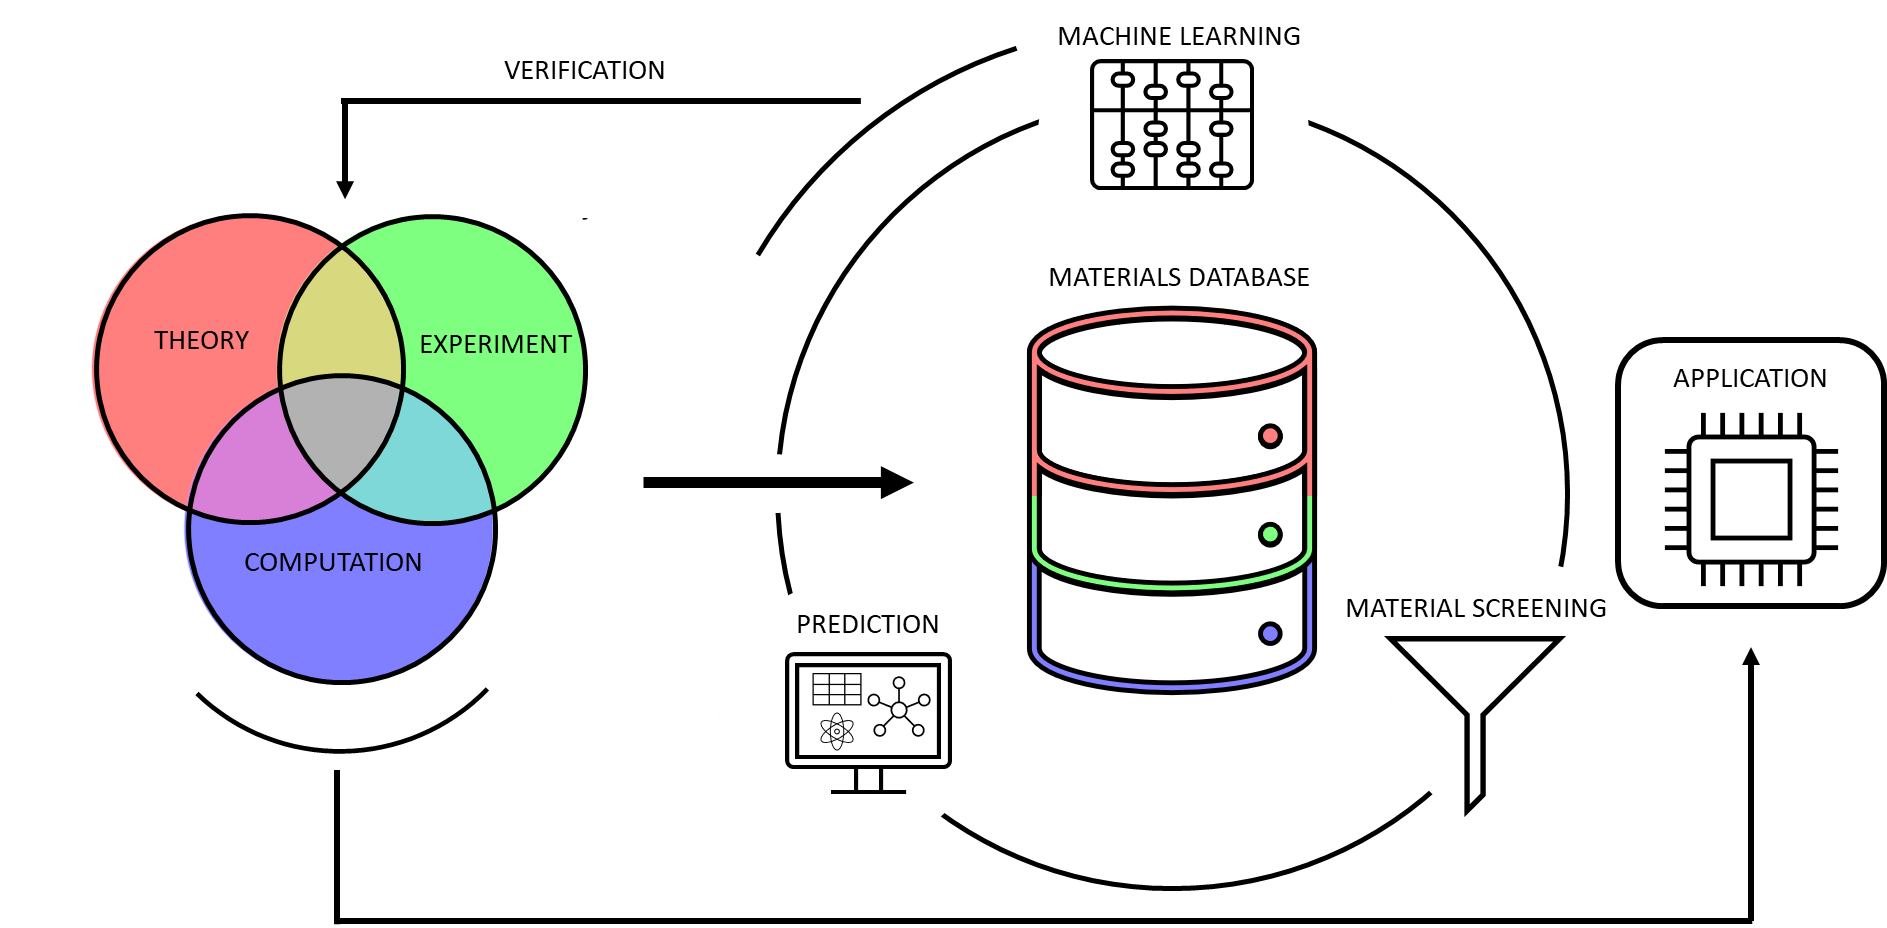
\includegraphics[width=0.9\textwidth]{figures/ht-workflow-new-2.png}
    \caption{Schematic of an example workflow in material informatics. Results from theory, experiment and computation are fed into material databases (arrow pointing to the center). A cycle involving material screening, machine learning and predictions leads to knowledge gain and ultimately applications in fields such as clean energy and quantum technology. 
    }
    \label{fig:ht-workflow}
\end{figure}

Several platforms are available for the development of quantum technologies (QT), but the materials and fabrication technologies are less mature than those for, e.g., classical computers and sensors. 
An important concern in this context is that of scalability. 
For example, the best performing quantum computer prototypes available today rely on superconducting electronics or trapped ions. Both technologies require millikelvin temperatures to operate, fabrication is challenging, and the stability of interactions between qubits is an issue. Instead, semiconductors are emerging as a promising alternative platform, offering competitive characteristics combined with the possibility of room temperature operation and mature and scalable material processing and fabrication.  

Quantum technologies based on semiconductors rely on either defects or quantum dots where the latter kind can be of the self-assembled or fabricated type. 
Semiconductor defects can act as single-photon emitters or spin centers and are compatible with the three main QT categories of computing, communication and sensing.  
These characteristics are most often found for the case of defects that introduce deep energy levels into the semiconductor band gap. So-called deep level defects can trap charge carriers in localized states that are essentially isolated from the surroundings, making them highly suitable for QT due to, e.g., indistinguishable single-photon emission and long spin coherence times. 
The most well-known quantum compatible defect is the negatively charged nitrogen-vacancy (NV) center in diamond \cite{Doherty_2013}, but silicon carbide (SiC) and the various quantum emitters therein are strong contenders in certain areas due to the favorable emission wavelength region in the near infrared coupled with more mature material processing and fabrication \cite{Bathen2021}. 
However, defect based QT is still in the early stages, and the issues left to address include identification of suitable host materials and candidate defects, and scalable and reproducible quantum device fabrication. 
Furthermore, we lack a complete understanding of the requirements for a material to manifest quantum compatible properties,  
and the selection of known quantum compatible semiconductor host materials is slim. 

The majority of discoveries of QT compatible characteristics in semiconductors has so far happened by serendipity, and there is an urgent need for a better and more systematic understanding of how the QT compatible materials properties manifest. In this context, a framework for dedicated materials search and analysis is needed. 

The fourth science paradigm of big data driven science presents a significant improvement over the third paradigm focusing on computational science, for instance via density functional theory calculations of different materials properties. Instead, the fourth paradigm  introduces the potential of targeted search for promising material systems to enable properties such as coherent and isolated spin states and indistinguishable single-photon emission to manifest. 
Rather than searching through a host of signals for those that match our criteria, we are now able to \textit{predict} which materials and signatures we should target for more detailed studies, following the framework illustrated in Figure~\ref{fig:ht-workflow}. 
This is made feasible by the availability of databases containing material properties for a wide range of different systems. In this work, the data in question are provided by bulk density functional theory (DFT) calculations to obtain the ground state properties of different elements and compounds. Combined with machine learning methods we provide a path towards precise classification of qubit candidates. The inclusion of machine learning methods follows recent trends in applications of statistical learning, data science and machine learning for scientific discoveries, see for example Refs.~\cite{deiana2021,Carleo2019}.

In this work we provide a framework for the data mining and automated discovery of promising solid-state semiconductor hosts for quantum emitters and spin centers using targeted database search and machine learning methods combined with knowledge from the field. 
In this context, we do not distinguish between the specific mechanism giving rise to properties such as single-photon emission and long spin coherence times (e.g., semiconductor defects or quantum dots); instead, we attempt to target all materials that may accommodate the desired characteristics.  
The methodology developed herein can be modified for other material types and application areas provided that a large enough database with relevant theoretical and/or experimental data are available. 

The approach we have developed relies on data extraction from the databases Materials Project \cite{Jain2013,Jain2018}, the Open Quantum Materials Database (OQMD) \cite{Saal2013, Kirklin2015}, JARVIS-DFT \cite{Choudhary2020}, AFLOW \cite{Curtarolo2012, Curtarolo2012a, Calderon2015} and AFLOW-ML \cite{Isayev2017}. 
The Python library for data mining Matminer \cite{Ward2018} was then used for material analysis to featurize the extracted data. An important aspect of our work is the database building and pertinent development of the training sets for machine learning methods. We have developed three different approaches to data mining: (i) \emph{the Ferrenti approach} which is similar to that proposed by \citeauthor{Ferrenti2020} \cite{Ferrenti2020}, (ii) \emph{the augmented Ferrenti approach} and (iii) \emph{the intuitive approach}. We find that the former two methodologies base their data extraction protocols on broad material descriptors, leading to large sets of potentially suitable candidates \cite{Mehta2019,Hastie2009}. The third approach, on the other hand, relies on including materials with experimentally proven advantageous characteristics in the training set and therefore yields a narrower set of possible candidates. The three training sets where then analyzed with the four supervised machine learning methods logistic regression, decision trees, random forests and gradient boosting, and yielded $214$ predicted candidates 
%(to a $0.5$ cut-off)  
with examples such as ZnGeP$_2$, MgSe, CdS, BP, BC$_2$N, BP, Ge, GeC, InP, and InAs. 
Focused theoretical and experimental studies, using methods such as, e.g., density functional theory, photoluminescence spectroscopy and optically detected magnetic resonance, are needed to verify the predictions that quantum properties may manifest as a result of defects or nanostructures in the above listed materials. 

\section*{Results}

\subsection*{Information Flow} 

The information stream in this work can be regarded as many modular parts 
%connected in logical pieces. 
%MHJ What do we mean with logical pieces? 
that are connected. 
The initial step for gathering material data and building features is visualized by the  flowchart in Figure~\ref{fig:flowchart}. 
Initially, we start by extracting all entries in the Materials Project (MP) database that match a specific query. 
The MP database contains ground state properties of different materials that are computed using density functional theory (DFT). The DFT calculations in the database were performed using the Vienna ab initio simulation package (VASP) \cite{Kresse1996} and the Perdew-Burke-Ernzerhof (PBE) \cite{Perdew1996} exchange-correlation functional to calculate the electronic structure of the materials. 

\begin{figure}[t]
    \centering
    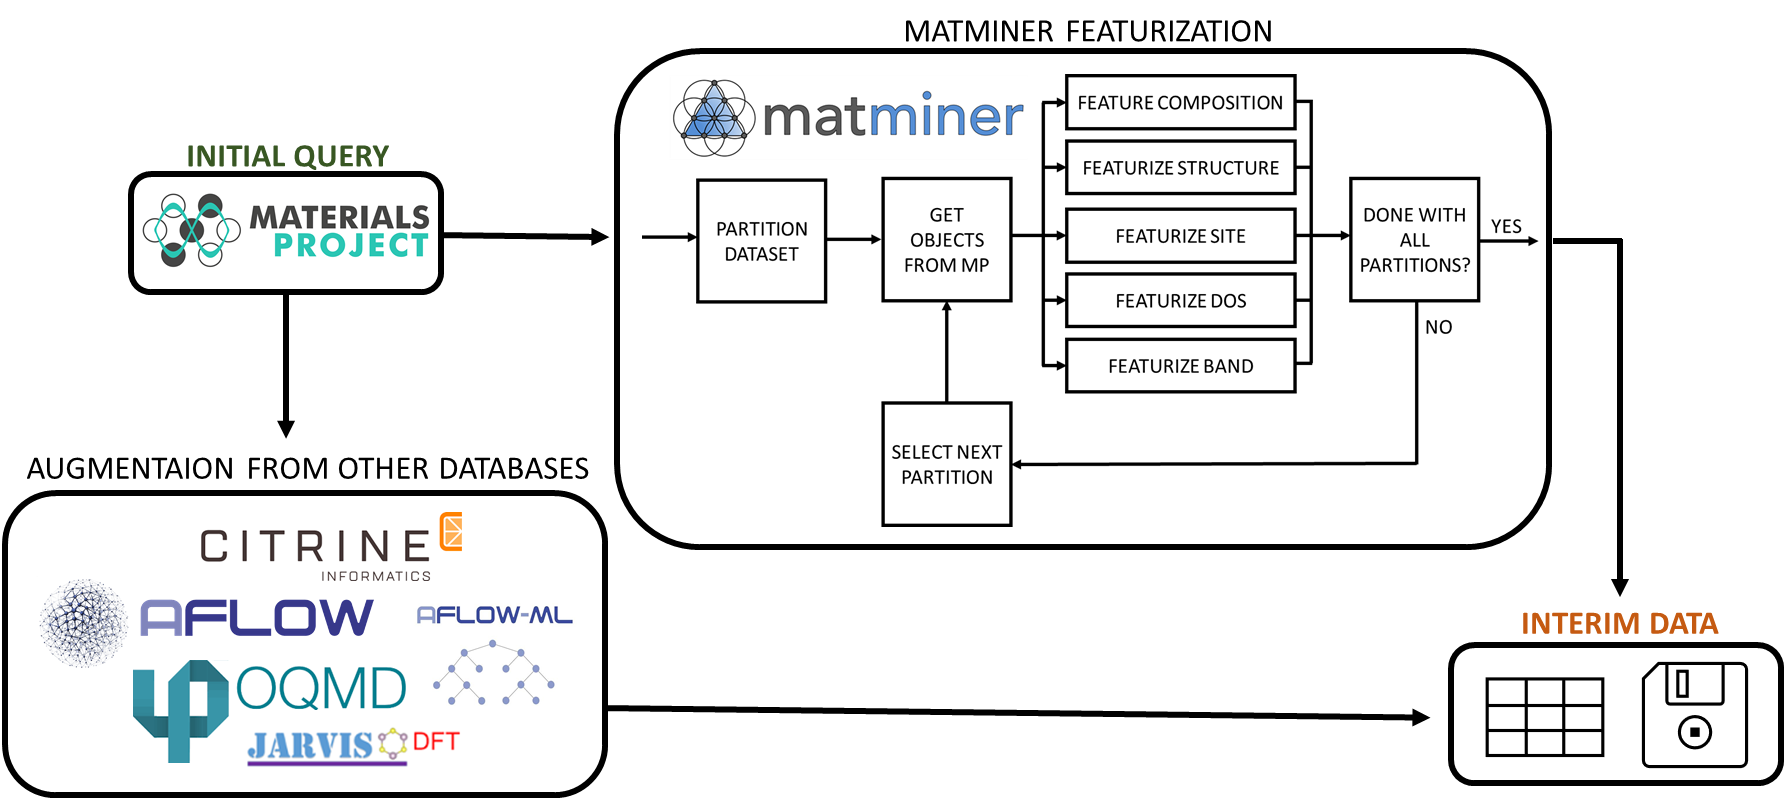
\includegraphics[width=0.9\textwidth]{figures/flow_chart.png}
    \caption{The data flow of the main project, starting from an initial MP query, and ending with a featurized dataset with entries from several other databases. To limit the memory and computational usage, the data are partitioned into smaller subsets where the respective Pymatgen objects  
    (Pymatgen is a robust, open-source Python library for materials analysis \cite{pymatgen}) 
    are obtained through a query to be used in the following featurization steps. This process is repeated iteratively until all the data has been featurized. Abbreviations used are Materials Project (MP), density of states (DOS) and electronic band structure (band).
    }
    \label{fig:flowchart}
\end{figure}

The conditions for the initial MP query are that the materials must derive from 
%experimental data 
the ICSD database and have a band gap wider than $0.1$~eV to exclude metallic compounds. The Inorganic Crystal Structure Database (ICSD) is the world's largest database for completely identified inorganic crystal structures \cite{Allen1987,Zagorac2019}. 
%OH: corrected icsd citation to german one (different from nist)
In a parallel step, entries that are deemed similar to the entries from the initial query are extracted from the databases OQMD \cite{Saal2013,Kirklin2015}, JARVIS-DFT \cite{Choudhary2020}, AFLOW \cite{Curtarolo2012, Curtarolo2012a, Calderon2015}, AFLOW-ML \cite{Isayev2017} and the Citrination platform \cite{OMaraJordan2016MDIA}. The results of these steps are combined into a data set for further analysis. 

Thereafter, we apply Matminer’s \cite{Ward2018} featurization tools to generate thousands of features from the data. 
Before applying any machine learning algorithm, the data was transformed into a numerical representation that reflects the relationship between the input and output data. This transformation is known as generating descriptors 
or features, however, we will in this work adapt the name featurization. 
The open-source library of Matminer provides many tools to featurize existing features extracted from the Materials Project. 
%MB I moved the below to methods 
%To apply Matminer's featurization tools, we extend an existing implementation by \citeauthor{Breuck2021} \cite{Breuck2021}, which were used to generate a supervised machine learning framework called the MODnet. Their implementation provides featurization for a material's composition, structure and atomic sites. However, Matminer also provides featurization tools for a material's density of states (DOS) and band structure, therefore, we extend their implementation to facilitate such featurizations. 
A schematic visualizing the featurization process in Matminer is contained in Fig.~\ref{fig:flowchart} 
and focuses on a material's composition,  structure, atomic sites, density of states and band structure. 
The $39$ features selected as material descriptors in this work can be found in the Supplementary Material at \cite{supplementary}. The selection of features was kept rather wide as we do not precisely know which features best describe a solid state material platform for quantum technology. 

\subsection*{Data Mining}

After compiling a data set from the procedure outlined above, we face an obstacle in terms of defining a training set for the machine learning algorithms. This is challenging for two reasons.  
Firstly, although QT compatible properties are becoming increasingly well studied for the case of, e.g., nitrogen-vacancy centers in diamond, single-photon emitters in silicon carbide and quantum dot structures, few candidate materials are known. An additional consideration is that the physical mechanisms promoting favorable properties are not fully understood, neither for the case of defect- or QD-based quantum technology. Secondly, defining materials as unsuitable candidates for QT has proven to be surprisingly intricate. 
We follow three separate procedures to define a training set consisting of materials that are labeled as both suitable and unsuitable candidates for QT. 

\subsubsection*{The Ferrenti approach}
The first approach to defining a training set is based on the criteria proposed by \citeauthor{Ferrenti2020} \cite{Ferrenti2020}.
They suggest a data mining process consisting of four stages by systematically evaluating the suitability of host materials from the Materials Project. In this framework, we label \textbf{suitable} candidates by the following steps: 
\begin{enumerate}
    \item Include materials that;
    \begin{itemize}
        \item contain elements with more than $50 \ \%$ natural abundance of spin zero isotopes,
        \item crystallize in non-polar space groups,
        \item are present in the ICSD database, 
        and
        \item are calculated to be nonmagnetic. 
    \end{itemize}
    \item Pragmatically remove toxic, radioactive and otherwise ``difficult'' materials;
    \begin{itemize}
        \item exclude Th, U, Cd and Hg because they are radioactive and/or toxic in the most stable forms,
        \item exclude any rare-earth metals (because of the difficulty of obtaining pure materials free of isotopes with nuclear spin) and noble gases (due to the lack of stable solid phases),
        \item exclude transition metal elements with unpaired electrons like Fe and Ni because of their paramagnetism. Ru and Os are also removed because they only exist in the data as complex cluster structures. 
    \end{itemize}
    \item Include only materials with a band gap larger than $0.5$~eV calculated using DFT and the PBE functional. The value of $0.5$~eV was chosen to match that typically predicted for silicon by PBE-level DFT calculations. 
    \item Ensure that energy above hull is less than $0.2$~eV per atom.
\end{enumerate}

The inclusion criteria are targeted primarily at semiconductors that can host deep level defects with spin qubit capabilities. In this context, long spin coherence times are needed, and the possibility of having an environment free of nuclear spins and permanent magnetism is therefore desirable. Additionally, to obtain defect-based single-photon emitters with sharp zero-phonon lines and indistinguishable photon emission, non-polar materials are assumed to be preferable. 
The inclusion criteria listed above are based on the work of \citeauthor{Weber2010} \cite{Weber2010}. 

Transition metal elements are eliminated in this approach if they have unpaired electrons because the presence of permanent electric dipole moments may have a detrimental impact on the optical coherence of defect emission. In this context, also the symmetry of the crystalline host may be important. Therefore, only phases which take on non polar space groups are considered in this approach. 
The energy above hull requirement is included to ensure that the selected compounds are thermodynamically stable. 

We then label \textbf{unsuitable} candidates according to the reverse requirements of the above; as materials in the ICSD database \cite{Allen1987,Zagorac2019} %MHJ need ref here
that crystallize in polar space groups, are calculated to be magnetic and have a band gap larger than $0.1$~eV (to exclude metals but include lower-band gap semiconductors) as calculated by DFT using the PBE functional, as discussed above.
The resulting complete training set contains $1581$ materials where %$56 \ \%$ 
$35 \ \%$
are labeled as unsuitable and 
%$44 \ \%$
$65 \ \%$
as suitable for QT applications.  

\subsubsection*{The augmented Ferrenti approach}
In the second approach, we adjust the former one in order to expand the training set beyond practical considerations. This approach is therefore named \emph{the augmented Ferrenti approach}. 

In the first approach we included criteria that were not physically motivated, but instead to some extent based on a practical perspective, such as excluding toxic and radioactive elements. Such criteria are not necessarily related to what makes a material suitable for quantum technology - eventually it is up to the experimentalist to decide the feasibility of the material to be employed. 
Consequently, in the augmented Ferrenti approach, we remove stage two from the approach above. Moreover, we include a few additional elements that have shown promising properties but were initially excluded due to the lack of spin zero isotopes. 

The following steps constitute the process of choosing \textbf{suitable} candidates in the \emph{augmented Ferrenti approach}:
\begin{enumerate}
    \item Include materials that; 
    \begin{itemize}
        \item contain elements where more than half have a natural abundance of spin zero isotopes, including Al, P, Ga, As, B and N, 
        \item crystallize in non-polar space groups,
        \item are present in the ICSD database,
        \item are calculated to be nonmagnetic. 
    \end{itemize}
    \item Only keep materials that have a band gap larger than $1.5$~eV as calculated by PBE-GGA. The higher band gap requirement (as compared to the Ferrenti approach) is included here to avoid including an unfeasible number of candidate materials. 
    \item Ensure that the energy above hull is less than $0.2$~eV per atom. 
\end{enumerate}

For \textbf{unsuitable} candidates, we implement the same strategy as for the first Ferrenti approach. The result is a somewhat unbalanced training set, with up to $75 \ \%$ of the materials found in the suitable group. However, the training set is $78 \ \%$ larger than for the Ferrenti approach with $2141$ suitable and $684$ unsuitable materials.

\subsubsection*{The intuitive approach}
The third approach differs substantially from the first two approaches in terms of material labeling, as we apply knowledge from the field (see for instance Refs.~\cite{Atatuere2018,Zhang2020,Son2020,Toth2019,Bathen2021} for an overview) to pick our promising material host candidates. 
In other words, we restrict ourselves to materials where quantum compatible properties have been either experimentally demonstrated or theoretically predicted. 
We therefore name this scheme \emph{the intuitive approach}. Due to the concern of having a training set that is too narrow in scope, we will also include some  materials that are promising in the sense that they have suitable properties for accommodating deep defects that can potentially exhibit quantum effects - even though such effects may not yet have been shown. These material choices were motivated by the criteria and predictions for QT compatible deep level defects defined by \citeauthor{Weber2010} \cite{Weber2010}. 
Materials where properties like single-photon emission and spin manipulation have been observed but attributed to quantum dots (formed by self-assembly or lithographic structuring) rather than being directly  defect related will also be included in this context.  
The approach to pick \textbf{suitable} candidates can be summed up as;   
\begin{enumerate}
    \item Pick candidates that match the formulas in Table~\ref{tab:qt-materials}, or the formulas ZnSe, AlP, GaP, AlAs, ZnTe, CdS \cite{Weber2010} or SiGe \cite{Hardy2019}. 
    \item Ensure that the candidates are present in the ICSD database.  
    \item Perform a manual screening for appropriate crystallographic structures. 
\end{enumerate}

\begin{table}[b]
    \centering 
    \caption{Overview of materials and defects that have been demonstrated to exhibit QT compatible characteristics such as single-photon emission and coherent spin manipulation.}
    \begin{tabular}{c|c|c|c}
    Material & Band gap (eV) & Defect candidates & References \\
    \hline
    Diamond  & $5.5$  & N$_\mathrm{C}V_\mathrm{C}$, Si$_\mathrm{C}V_\mathrm{C}$, Ge$_\mathrm{C}V_\mathrm{C}$ & \cite{Taylor2008,Balasubramanian_2009,Barclay2011,Gordon2013,Rogers_2014,Bhaskar_2018} \\ 
    SiC & $2.2$-$3.3$ & $V_\mathrm{Si}$, $V_\mathrm{Si}V_\mathrm{C}$, C$_\mathrm{Si}V_\mathrm{C}$, N$_\mathrm{C}V_\mathrm{Si}$ & \cite{Widmann2014,Christle_2015,Castelletto_2014,Zargaleh_2018}  \cite{Weber2010, Son2020, Falk2013} \\ 
    Si & $1.1$ & P, G, unidentified & \cite{Muhonen_2014,Durand_2020,Redjem2020} \\ 
    (2D) \textit{h}-BN & $6.0$ & Unidentified defects & \cite{Tran_2016,Tran_2016b,Hayee_2020} \\ 
    (2D) MoS$_2$, WSe$_2$, WS$_2$ & $<2.5$~eV & Bound excitons & \cite{Toth2019} \\
    ZnO & $3.4$ & Unidentified defects & \cite{Morfa2012} \\ 
    ZnS & $3.6$ (zincblende) & Unidentified defects & \cite{Stewart2019} \\ 
    GaAs & $1.4$ & Quantum dots & \cite{Bluhm2010} \\ 
    GaN & $3.4$ & Quantum dots, unidentified defects & \cite{Roux2017,Berhane2018} \\
    AlN & $6.0$ & Unidentified defects & \cite{Xue2020}\\
    \end{tabular}
    \label{tab:qt-materials}
\end{table} 

Table~\ref{tab:qt-materials} contains an overview of known semiconductor materials with demonstrated quantum compatible characteristics. In this context, we consider single-photon emission and coherent spin manipulation. The table forms the basis for picking suitable candidates for the intuitive approach. The properties being studied arise from mechanisms related to, e.g., point defects, bound excitons, and both self-assembled and lithographically structured quantum dots and nanostructures such as 2D materials. 
Quantum emission signatures have been assigned to specific defects in both diamond and SiC, but for most other materials, secure identification of the responsible defects or structure related mechanism is still lacking. 
In the intuitive approach, we include materials that are known to be quantum compatible as outlined in Table~\ref{tab:qt-materials} in the training set. Additionally, we also include materials matching the formulas ZnSe, AlP, GaP, AlAs, ZnTe, CdS and SiGe as these materials have been predicted to behave as suitable quantum hosts based on favorable properties such as a wide band gap and low spin-orbit coupling \cite{Weber2010,Hardy2019}.  

After the first stage of picking candidates we are left with a list of $202$ matching formulas which includes $12$ entries that have a band gap of less than $0.4$~eV. These $12$ entries are calculated to be thermodynamically unstable in terms of the energy above hull, and will decompose into other materials in the list --- incidentally, the resulting structures all have calculated band gaps that are substantially above $0.5$~eV. We include all of the $202$ structures except for C (mp-568410) which has a PBE-computed band gap of $0.12$~eV; i.e., a metal according to AFLOW-ML and it is therefore labeled as an unsuitable candidate. 
 
%% OH: Dirty details about suitable materials:
Entries matching the formulas C, SiC, BN, MoS$_2$, WSe$_2$ and WS$_2$ (quantum compatible characteristics have been demonstrated) were manually screened to see if the entries have a matching structure to the respective candidates discussed earlier and summarized in Table~\ref{tab:qt-materials}. 
For carbon, we admit three-dimensional diamond-like structures as explicitly stated in the column tags from the Materials Project. Additionally, we find several two-dimensional structures of carbon with a large band gap ($>1.5$~eV) among the data. We add these as suitable candidates. Complex structures (e.g., C$_{28}$, C$_{48}$ and C$_{60}$) were moved to the test set in our machine learning studies, see discussion below. For SiC we admitted all entries which included the $2$H, $3$C, $4$H, $6$H and $15$R polytypes. Concerning BN, MoS$_2$, WSe$_2$ and WS$_2$, we only admit two-dimensional structures. For non-matching structures not mentioned so far, we move them to the test set to see if they will be predicted as suitable or not by the machine learning methods that are applied in a later stage.

The materials AlP, GaP, AlAs, ZnTe and CdS were manually screened for tetrahedrally coordinated structures, and have been included since \citeauthor{Weber2010} \cite{Weber2010} identified them as potentially promising candidates due to suitable material properties. 
We note that only tetrahedrally coordinated structures of the given formulas were included in the training set after imposing the band gap restriction of $0.5$~eV. 

After the three screening steps in the intuitive approach, a total of $187$ entries were labeled as suitable candidates for the training set. 
Notably, the candidates labeled as suitable in the intuitive approach contain only compounds that are either elementary (unary) or binary. 
We want to avoid discriminating based on the number of elements in a compound, and therefore we remove the feature that describes the number of elements in a compound. 
%See the Supplementary Material at \cite{supplementary} for a table containing the manually screened materials that were labeled as suitable candidates in the training set for the intuitive approach. 
Since the training set constituting suitable candidates in the third approach contains rather few entries, we add $400$ candidates that are labeled as \emph{unsuitable}. These are picked at random from the pool of unsuitable candidates from the two previous approaches, in addition to those that were marked as unsuitable through the manual screening process. 

\subsubsection*{Comparing the approaches}
The three different approaches to data mining place a particular emphasis on each of their specific goals. The Ferrenti approach relies on choosing only elements with spin zero isotopes and compounds that crystallize in nonpolar spacegroups together with practical filters, while the augmented Ferrenti approach allows a larger variety of elements and removes the practical reasons for excluding candidate materials. Thus, the first approach targets a more narrow prediction space than the second approach does. However, perhaps the most restricted approach is the intuitive one. Since the variety of known suitable materials is substantially more restricted than for the two other approaches, we would expect the intuitive approach to provide an even narrower prediction space. %Here, one should keep in mind that ... 

Taking a closer look at the training set from the Ferrenti approach, we find that carbon in a diamond-like structure is classified as a suitable candidate. This is in good agreement with experimental observations (see Table~\ref{tab:qt-materials}) and hence also with the candidates that were manually defined as suitable in the intuitive approach.  
Interestingly, in the training set from the Ferrenti approach, we find that carbon in two-dimensional graphite-like structures are labeled as suitable as well. All structures of silicon are also labeled as suitable together with one entry of silicon carbide. Note that this is the 3C polytype of SiC, meaning that the most quantum compatible SiC polytype, 4H-SiC, is missing from the training set. Among other potentially suitable candidates we find ZnS, ZnSe, ZnO and ZnTe present in the training data. 

In the training set of the Augmented Ferrenti approach, we find a single entry for each of SiC, Si, GaN, ZnS, GaP, AlAs and AlP, carbon in both diamond- and graphite-like structures, and AlN in three different configurations. The training set includes a larger variety of 
materials that are known to be quantum compatible as compared to the Ferrenti approach due to admitting more elements in the initial selection process. However, since we also included a more stringent band gap restriction of $1.5$~eV (to restrict the amount of materials in the training set), we find a more sparse representation of each known chemical formula present in the training set. 

We provide a visualization of each approach's training data as a parallel coordinate plot for a few selected features in Figure~\ref{fig:parallel-coordinates-approaches}. Parallel coordinate schemes \cite{Inselberga1990, Inselberg1985} represent a multi-dimensional data tuple as one polyline crossing a parallel axis. The selected features are found on the x-axis, while the y-axis shows the value of the data. Thus, parallel coordinate plots can turn many-dimensional data into a compact  two-dimensional representation. Due to possible data cluttering, the figure visualizes a random sample of each class (suitable or unsuitable) with an upper limit of $250$ per class with transparent lines. The green and red polylines represent suitable and unsuitable candidates, respectively. 

The Ferrenti approach and the augmented Ferrenti approach share several similarities. 
Interestingly, we observe that the entries in Fig.~\ref{fig:parallel-coordinates-approaches} span roughly the same dimensions for the Ferrenti and augmented Ferrenti approaches, despite the more restricted nature of the former.  
The two approaches' upper limits for ionic character and covalent range are very similar in the case of candidates labeled as both suitable and unsuitable.   
Moreover, all candidates that were labeled as unsuitable exhibit polar space groups (follows from the definition of the training sets), and the two approaches also share that suitable candidates can consist of up to five different elements. 

The biggest difference is found for the intuitive approach. The entries labeled as suitable candidates do not exhibit any magnetization, even though the materials crystallize in both polar and non-polar space groups - contrarily to the two Ferrenti-based approaches. Moreover, we observe that the range of covalent radius and maximum ionic character span a substantially smaller parameter space in the case of the intuitive approach than for the two former ones.  
Here, we can begin to deduce some trends, if the findings from the intuitive approach are taken as guidance. Where the polarity of the material's space group may be less important than assumed in the Ferrenti based approaches, ionic character and covalent range are distinguished from the other features visualized in Fig.~\ref{fig:parallel-coordinates-approaches}. 
Identification of the features that promote quantum compatible  characteristics could be crucial for targeted quantum device design based on careful material selection, nanostructuring and defect engineering. 

\begin{figure}[t] %!htp
    \centering
    \begin{subfigure}{1\textwidth}
        \centering
          %% Creator: Matplotlib, PGF backend
%%
%% To include the figure in your LaTeX document, write
%%   \input{<filename>.pgf}
%%
%% Make sure the required packages are loaded in your preamble
%%   \usepackage{pgf}
%%
%% and, on pdftex
%%   \usepackage[utf8]{inputenc}\DeclareUnicodeCharacter{2212}{-}
%%
%% or, on luatex and xetex
%%   \usepackage{unicode-math}
%%
%% Figures using additional raster images can only be included by \input if
%% they are in the same directory as the main LaTeX file. For loading figures
%% from other directories you can use the `import` package
%%   \usepackage{import}
%%
%% and then include the figures with
%%   \import{<path to file>}{<filename>.pgf}
%%
%% Matplotlib used the following preamble
%%   \usepackage[detect-all,locale=DE]{siunitx} \usepackage[T1]{fontenc} \usepackage[utf8x]{inputenc}
%%
\begingroup%
\makeatletter%
\begin{pgfpicture}%
\pgfpathrectangle{\pgfpointorigin}{\pgfqpoint{5.584949in}{2.190539in}}%
\pgfusepath{use as bounding box, clip}%
\begin{pgfscope}%
\pgfsetbuttcap%
\pgfsetmiterjoin%
\pgfsetlinewidth{0.000000pt}%
\definecolor{currentstroke}{rgb}{1.000000,1.000000,1.000000}%
\pgfsetstrokecolor{currentstroke}%
\pgfsetstrokeopacity{0.000000}%
\pgfsetdash{}{0pt}%
\pgfpathmoveto{\pgfqpoint{0.000000in}{0.000000in}}%
\pgfpathlineto{\pgfqpoint{5.584949in}{0.000000in}}%
\pgfpathlineto{\pgfqpoint{5.584949in}{2.190539in}}%
\pgfpathlineto{\pgfqpoint{0.000000in}{2.190539in}}%
\pgfpathclose%
\pgfusepath{}%
\end{pgfscope}%
\begin{pgfscope}%
\pgfsetbuttcap%
\pgfsetmiterjoin%
\definecolor{currentfill}{rgb}{1.000000,1.000000,1.000000}%
\pgfsetfillcolor{currentfill}%
\pgfsetlinewidth{0.000000pt}%
\definecolor{currentstroke}{rgb}{0.000000,0.000000,0.000000}%
\pgfsetstrokecolor{currentstroke}%
\pgfsetstrokeopacity{0.000000}%
\pgfsetdash{}{0pt}%
\pgfpathmoveto{\pgfqpoint{0.377421in}{0.128033in}}%
\pgfpathlineto{\pgfqpoint{5.264131in}{0.128033in}}%
\pgfpathlineto{\pgfqpoint{5.264131in}{1.607731in}}%
\pgfpathlineto{\pgfqpoint{0.377421in}{1.607731in}}%
\pgfpathclose%
\pgfusepath{fill}%
\end{pgfscope}%
\begin{pgfscope}%
\pgfpathrectangle{\pgfqpoint{0.377421in}{0.128033in}}{\pgfqpoint{4.886710in}{1.479697in}}%
\pgfusepath{clip}%
\pgfsetbuttcap%
\pgfsetmiterjoin%
\pgfsetlinewidth{0.501875pt}%
\definecolor{currentstroke}{rgb}{1.000000,0.388235,0.278431}%
\pgfsetstrokecolor{currentstroke}%
\pgfsetstrokeopacity{0.200000}%
\pgfsetdash{}{0pt}%
\pgfpathmoveto{\pgfqpoint{0.377421in}{1.540472in}}%
\pgfpathcurveto{\pgfqpoint{0.703201in}{1.540472in}}{\pgfqpoint{1.028982in}{0.255216in}}{\pgfqpoint{1.354763in}{0.255216in}}%
\pgfpathcurveto{\pgfqpoint{1.680543in}{0.255216in}}{\pgfqpoint{2.006324in}{0.891527in}}{\pgfqpoint{2.332105in}{0.891527in}}%
\pgfpathcurveto{\pgfqpoint{2.657886in}{0.891527in}}{\pgfqpoint{2.983666in}{0.921833in}}{\pgfqpoint{3.309447in}{0.921833in}}%
\pgfpathcurveto{\pgfqpoint{3.635228in}{0.921833in}}{\pgfqpoint{3.961008in}{1.271436in}}{\pgfqpoint{4.286789in}{1.271436in}}%
\pgfpathcurveto{\pgfqpoint{4.612570in}{1.271436in}}{\pgfqpoint{4.938350in}{0.969293in}}{\pgfqpoint{5.264131in}{0.969293in}}%
\pgfusepath{stroke}%
\end{pgfscope}%
\begin{pgfscope}%
\pgfpathrectangle{\pgfqpoint{0.377421in}{0.128033in}}{\pgfqpoint{4.886710in}{1.479697in}}%
\pgfusepath{clip}%
\pgfsetbuttcap%
\pgfsetmiterjoin%
\pgfsetlinewidth{0.501875pt}%
\definecolor{currentstroke}{rgb}{1.000000,0.388235,0.278431}%
\pgfsetstrokecolor{currentstroke}%
\pgfsetstrokeopacity{0.200000}%
\pgfsetdash{}{0pt}%
\pgfpathmoveto{\pgfqpoint{0.377421in}{1.540472in}}%
\pgfpathcurveto{\pgfqpoint{0.703201in}{1.540472in}}{\pgfqpoint{1.028982in}{0.210041in}}{\pgfqpoint{1.354763in}{0.210041in}}%
\pgfpathcurveto{\pgfqpoint{1.680543in}{0.210041in}}{\pgfqpoint{2.006324in}{0.518210in}}{\pgfqpoint{2.332105in}{0.518210in}}%
\pgfpathcurveto{\pgfqpoint{2.657886in}{0.518210in}}{\pgfqpoint{2.983666in}{0.792350in}}{\pgfqpoint{3.309447in}{0.792350in}}%
\pgfpathcurveto{\pgfqpoint{3.635228in}{0.792350in}}{\pgfqpoint{3.961008in}{0.733364in}}{\pgfqpoint{4.286789in}{0.733364in}}%
\pgfpathcurveto{\pgfqpoint{4.612570in}{0.733364in}}{\pgfqpoint{4.938350in}{0.205942in}}{\pgfqpoint{5.264131in}{0.205942in}}%
\pgfusepath{stroke}%
\end{pgfscope}%
\begin{pgfscope}%
\pgfpathrectangle{\pgfqpoint{0.377421in}{0.128033in}}{\pgfqpoint{4.886710in}{1.479697in}}%
\pgfusepath{clip}%
\pgfsetbuttcap%
\pgfsetmiterjoin%
\pgfsetlinewidth{0.501875pt}%
\definecolor{currentstroke}{rgb}{1.000000,0.388235,0.278431}%
\pgfsetstrokecolor{currentstroke}%
\pgfsetstrokeopacity{0.200000}%
\pgfsetdash{}{0pt}%
\pgfpathmoveto{\pgfqpoint{0.377421in}{1.540472in}}%
\pgfpathcurveto{\pgfqpoint{0.703201in}{1.540472in}}{\pgfqpoint{1.028982in}{0.299886in}}{\pgfqpoint{1.354763in}{0.299886in}}%
\pgfpathcurveto{\pgfqpoint{1.680543in}{0.299886in}}{\pgfqpoint{2.006324in}{0.518210in}}{\pgfqpoint{2.332105in}{0.518210in}}%
\pgfpathcurveto{\pgfqpoint{2.657886in}{0.518210in}}{\pgfqpoint{2.983666in}{1.396602in}}{\pgfqpoint{3.309447in}{1.396602in}}%
\pgfpathcurveto{\pgfqpoint{3.635228in}{1.396602in}}{\pgfqpoint{3.961008in}{0.733364in}}{\pgfqpoint{4.286789in}{0.733364in}}%
\pgfpathcurveto{\pgfqpoint{4.612570in}{0.733364in}}{\pgfqpoint{4.938350in}{0.229818in}}{\pgfqpoint{5.264131in}{0.229818in}}%
\pgfusepath{stroke}%
\end{pgfscope}%
\begin{pgfscope}%
\pgfpathrectangle{\pgfqpoint{0.377421in}{0.128033in}}{\pgfqpoint{4.886710in}{1.479697in}}%
\pgfusepath{clip}%
\pgfsetbuttcap%
\pgfsetmiterjoin%
\pgfsetlinewidth{0.501875pt}%
\definecolor{currentstroke}{rgb}{1.000000,0.388235,0.278431}%
\pgfsetstrokecolor{currentstroke}%
\pgfsetstrokeopacity{0.200000}%
\pgfsetdash{}{0pt}%
\pgfpathmoveto{\pgfqpoint{0.377421in}{1.540472in}}%
\pgfpathcurveto{\pgfqpoint{0.703201in}{1.540472in}}{\pgfqpoint{1.028982in}{0.299946in}}{\pgfqpoint{1.354763in}{0.299946in}}%
\pgfpathcurveto{\pgfqpoint{1.680543in}{0.299946in}}{\pgfqpoint{2.006324in}{1.325605in}}{\pgfqpoint{2.332105in}{1.325605in}}%
\pgfpathcurveto{\pgfqpoint{2.657886in}{1.325605in}}{\pgfqpoint{2.983666in}{1.130444in}}{\pgfqpoint{3.309447in}{1.130444in}}%
\pgfpathcurveto{\pgfqpoint{3.635228in}{1.130444in}}{\pgfqpoint{3.961008in}{1.002400in}}{\pgfqpoint{4.286789in}{1.002400in}}%
\pgfpathcurveto{\pgfqpoint{4.612570in}{1.002400in}}{\pgfqpoint{4.938350in}{0.842391in}}{\pgfqpoint{5.264131in}{0.842391in}}%
\pgfusepath{stroke}%
\end{pgfscope}%
\begin{pgfscope}%
\pgfpathrectangle{\pgfqpoint{0.377421in}{0.128033in}}{\pgfqpoint{4.886710in}{1.479697in}}%
\pgfusepath{clip}%
\pgfsetbuttcap%
\pgfsetmiterjoin%
\pgfsetlinewidth{0.501875pt}%
\definecolor{currentstroke}{rgb}{1.000000,0.388235,0.278431}%
\pgfsetstrokecolor{currentstroke}%
\pgfsetstrokeopacity{0.200000}%
\pgfsetdash{}{0pt}%
\pgfpathmoveto{\pgfqpoint{0.377421in}{1.540472in}}%
\pgfpathcurveto{\pgfqpoint{0.703201in}{1.540472in}}{\pgfqpoint{1.028982in}{0.509186in}}{\pgfqpoint{1.354763in}{0.509186in}}%
\pgfpathcurveto{\pgfqpoint{1.680543in}{0.509186in}}{\pgfqpoint{2.006324in}{1.352950in}}{\pgfqpoint{2.332105in}{1.352950in}}%
\pgfpathcurveto{\pgfqpoint{2.657886in}{1.352950in}}{\pgfqpoint{2.983666in}{0.914639in}}{\pgfqpoint{3.309447in}{0.914639in}}%
\pgfpathcurveto{\pgfqpoint{3.635228in}{0.914639in}}{\pgfqpoint{3.961008in}{1.002400in}}{\pgfqpoint{4.286789in}{1.002400in}}%
\pgfpathcurveto{\pgfqpoint{4.612570in}{1.002400in}}{\pgfqpoint{4.938350in}{0.655862in}}{\pgfqpoint{5.264131in}{0.655862in}}%
\pgfusepath{stroke}%
\end{pgfscope}%
\begin{pgfscope}%
\pgfpathrectangle{\pgfqpoint{0.377421in}{0.128033in}}{\pgfqpoint{4.886710in}{1.479697in}}%
\pgfusepath{clip}%
\pgfsetbuttcap%
\pgfsetmiterjoin%
\pgfsetlinewidth{0.501875pt}%
\definecolor{currentstroke}{rgb}{1.000000,0.388235,0.278431}%
\pgfsetstrokecolor{currentstroke}%
\pgfsetstrokeopacity{0.200000}%
\pgfsetdash{}{0pt}%
\pgfpathmoveto{\pgfqpoint{0.377421in}{1.540472in}}%
\pgfpathcurveto{\pgfqpoint{0.703201in}{1.540472in}}{\pgfqpoint{1.028982in}{0.255078in}}{\pgfqpoint{1.354763in}{0.255078in}}%
\pgfpathcurveto{\pgfqpoint{1.680543in}{0.255078in}}{\pgfqpoint{2.006324in}{1.313398in}}{\pgfqpoint{2.332105in}{1.313398in}}%
\pgfpathcurveto{\pgfqpoint{2.657886in}{1.313398in}}{\pgfqpoint{2.983666in}{0.475838in}}{\pgfqpoint{3.309447in}{0.475838in}}%
\pgfpathcurveto{\pgfqpoint{3.635228in}{0.475838in}}{\pgfqpoint{3.961008in}{0.733364in}}{\pgfqpoint{4.286789in}{0.733364in}}%
\pgfpathcurveto{\pgfqpoint{4.612570in}{0.733364in}}{\pgfqpoint{4.938350in}{0.534807in}}{\pgfqpoint{5.264131in}{0.534807in}}%
\pgfusepath{stroke}%
\end{pgfscope}%
\begin{pgfscope}%
\pgfpathrectangle{\pgfqpoint{0.377421in}{0.128033in}}{\pgfqpoint{4.886710in}{1.479697in}}%
\pgfusepath{clip}%
\pgfsetbuttcap%
\pgfsetmiterjoin%
\pgfsetlinewidth{0.501875pt}%
\definecolor{currentstroke}{rgb}{1.000000,0.388235,0.278431}%
\pgfsetstrokecolor{currentstroke}%
\pgfsetstrokeopacity{0.200000}%
\pgfsetdash{}{0pt}%
\pgfpathmoveto{\pgfqpoint{0.377421in}{1.540472in}}%
\pgfpathcurveto{\pgfqpoint{0.703201in}{1.540472in}}{\pgfqpoint{1.028982in}{0.225185in}}{\pgfqpoint{1.354763in}{0.225185in}}%
\pgfpathcurveto{\pgfqpoint{1.680543in}{0.225185in}}{\pgfqpoint{2.006324in}{1.028930in}}{\pgfqpoint{2.332105in}{1.028930in}}%
\pgfpathcurveto{\pgfqpoint{2.657886in}{1.028930in}}{\pgfqpoint{2.983666in}{0.900253in}}{\pgfqpoint{3.309447in}{0.900253in}}%
\pgfpathcurveto{\pgfqpoint{3.635228in}{0.900253in}}{\pgfqpoint{3.961008in}{0.733364in}}{\pgfqpoint{4.286789in}{0.733364in}}%
\pgfpathcurveto{\pgfqpoint{4.612570in}{0.733364in}}{\pgfqpoint{4.938350in}{0.772052in}}{\pgfqpoint{5.264131in}{0.772052in}}%
\pgfusepath{stroke}%
\end{pgfscope}%
\begin{pgfscope}%
\pgfpathrectangle{\pgfqpoint{0.377421in}{0.128033in}}{\pgfqpoint{4.886710in}{1.479697in}}%
\pgfusepath{clip}%
\pgfsetbuttcap%
\pgfsetmiterjoin%
\pgfsetlinewidth{0.501875pt}%
\definecolor{currentstroke}{rgb}{1.000000,0.388235,0.278431}%
\pgfsetstrokecolor{currentstroke}%
\pgfsetstrokeopacity{0.200000}%
\pgfsetdash{}{0pt}%
\pgfpathmoveto{\pgfqpoint{0.377421in}{1.540472in}}%
\pgfpathcurveto{\pgfqpoint{0.703201in}{1.540472in}}{\pgfqpoint{1.028982in}{0.210237in}}{\pgfqpoint{1.354763in}{0.210237in}}%
\pgfpathcurveto{\pgfqpoint{1.680543in}{0.210237in}}{\pgfqpoint{2.006324in}{1.160176in}}{\pgfqpoint{2.332105in}{1.160176in}}%
\pgfpathcurveto{\pgfqpoint{2.657886in}{1.160176in}}{\pgfqpoint{2.983666in}{0.871479in}}{\pgfqpoint{3.309447in}{0.871479in}}%
\pgfpathcurveto{\pgfqpoint{3.635228in}{0.871479in}}{\pgfqpoint{3.961008in}{0.733364in}}{\pgfqpoint{4.286789in}{0.733364in}}%
\pgfpathcurveto{\pgfqpoint{4.612570in}{0.733364in}}{\pgfqpoint{4.938350in}{0.275076in}}{\pgfqpoint{5.264131in}{0.275076in}}%
\pgfusepath{stroke}%
\end{pgfscope}%
\begin{pgfscope}%
\pgfpathrectangle{\pgfqpoint{0.377421in}{0.128033in}}{\pgfqpoint{4.886710in}{1.479697in}}%
\pgfusepath{clip}%
\pgfsetbuttcap%
\pgfsetmiterjoin%
\pgfsetlinewidth{0.501875pt}%
\definecolor{currentstroke}{rgb}{1.000000,0.388235,0.278431}%
\pgfsetstrokecolor{currentstroke}%
\pgfsetstrokeopacity{0.200000}%
\pgfsetdash{}{0pt}%
\pgfpathmoveto{\pgfqpoint{0.377421in}{1.540472in}}%
\pgfpathcurveto{\pgfqpoint{0.703201in}{1.540472in}}{\pgfqpoint{1.028982in}{0.195295in}}{\pgfqpoint{1.354763in}{0.195295in}}%
\pgfpathcurveto{\pgfqpoint{1.680543in}{0.195295in}}{\pgfqpoint{2.006324in}{0.552804in}}{\pgfqpoint{2.332105in}{0.552804in}}%
\pgfpathcurveto{\pgfqpoint{2.657886in}{0.552804in}}{\pgfqpoint{2.983666in}{1.152024in}}{\pgfqpoint{3.309447in}{1.152024in}}%
\pgfpathcurveto{\pgfqpoint{3.635228in}{1.152024in}}{\pgfqpoint{3.961008in}{0.733364in}}{\pgfqpoint{4.286789in}{0.733364in}}%
\pgfpathcurveto{\pgfqpoint{4.612570in}{0.733364in}}{\pgfqpoint{4.938350in}{0.199483in}}{\pgfqpoint{5.264131in}{0.199483in}}%
\pgfusepath{stroke}%
\end{pgfscope}%
\begin{pgfscope}%
\pgfpathrectangle{\pgfqpoint{0.377421in}{0.128033in}}{\pgfqpoint{4.886710in}{1.479697in}}%
\pgfusepath{clip}%
\pgfsetbuttcap%
\pgfsetmiterjoin%
\pgfsetlinewidth{0.501875pt}%
\definecolor{currentstroke}{rgb}{1.000000,0.388235,0.278431}%
\pgfsetstrokecolor{currentstroke}%
\pgfsetstrokeopacity{0.200000}%
\pgfsetdash{}{0pt}%
\pgfpathmoveto{\pgfqpoint{0.377421in}{1.540472in}}%
\pgfpathcurveto{\pgfqpoint{0.703201in}{1.540472in}}{\pgfqpoint{1.028982in}{0.195459in}}{\pgfqpoint{1.354763in}{0.195459in}}%
\pgfpathcurveto{\pgfqpoint{1.680543in}{0.195459in}}{\pgfqpoint{2.006324in}{1.392711in}}{\pgfqpoint{2.332105in}{1.392711in}}%
\pgfpathcurveto{\pgfqpoint{2.657886in}{1.392711in}}{\pgfqpoint{2.983666in}{1.432569in}}{\pgfqpoint{3.309447in}{1.432569in}}%
\pgfpathcurveto{\pgfqpoint{3.635228in}{1.432569in}}{\pgfqpoint{3.961008in}{1.271436in}}{\pgfqpoint{4.286789in}{1.271436in}}%
\pgfpathcurveto{\pgfqpoint{4.612570in}{1.271436in}}{\pgfqpoint{4.938350in}{0.311073in}}{\pgfqpoint{5.264131in}{0.311073in}}%
\pgfusepath{stroke}%
\end{pgfscope}%
\begin{pgfscope}%
\pgfpathrectangle{\pgfqpoint{0.377421in}{0.128033in}}{\pgfqpoint{4.886710in}{1.479697in}}%
\pgfusepath{clip}%
\pgfsetbuttcap%
\pgfsetmiterjoin%
\pgfsetlinewidth{0.501875pt}%
\definecolor{currentstroke}{rgb}{1.000000,0.388235,0.278431}%
\pgfsetstrokecolor{currentstroke}%
\pgfsetstrokeopacity{0.200000}%
\pgfsetdash{}{0pt}%
\pgfpathmoveto{\pgfqpoint{0.377421in}{1.540472in}}%
\pgfpathcurveto{\pgfqpoint{0.703201in}{1.540472in}}{\pgfqpoint{1.028982in}{0.240061in}}{\pgfqpoint{1.354763in}{0.240061in}}%
\pgfpathcurveto{\pgfqpoint{1.680543in}{0.240061in}}{\pgfqpoint{2.006324in}{1.321568in}}{\pgfqpoint{2.332105in}{1.321568in}}%
\pgfpathcurveto{\pgfqpoint{2.657886in}{1.321568in}}{\pgfqpoint{2.983666in}{0.972187in}}{\pgfqpoint{3.309447in}{0.972187in}}%
\pgfpathcurveto{\pgfqpoint{3.635228in}{0.972187in}}{\pgfqpoint{3.961008in}{1.002400in}}{\pgfqpoint{4.286789in}{1.002400in}}%
\pgfpathcurveto{\pgfqpoint{4.612570in}{1.002400in}}{\pgfqpoint{4.938350in}{0.850752in}}{\pgfqpoint{5.264131in}{0.850752in}}%
\pgfusepath{stroke}%
\end{pgfscope}%
\begin{pgfscope}%
\pgfpathrectangle{\pgfqpoint{0.377421in}{0.128033in}}{\pgfqpoint{4.886710in}{1.479697in}}%
\pgfusepath{clip}%
\pgfsetbuttcap%
\pgfsetmiterjoin%
\pgfsetlinewidth{0.501875pt}%
\definecolor{currentstroke}{rgb}{1.000000,0.388235,0.278431}%
\pgfsetstrokecolor{currentstroke}%
\pgfsetstrokeopacity{0.200000}%
\pgfsetdash{}{0pt}%
\pgfpathmoveto{\pgfqpoint{0.377421in}{1.540472in}}%
\pgfpathcurveto{\pgfqpoint{0.703201in}{1.540472in}}{\pgfqpoint{1.028982in}{0.210239in}}{\pgfqpoint{1.354763in}{0.210239in}}%
\pgfpathcurveto{\pgfqpoint{1.680543in}{0.210239in}}{\pgfqpoint{2.006324in}{1.275021in}}{\pgfqpoint{2.332105in}{1.275021in}}%
\pgfpathcurveto{\pgfqpoint{2.657886in}{1.275021in}}{\pgfqpoint{2.983666in}{1.439763in}}{\pgfqpoint{3.309447in}{1.439763in}}%
\pgfpathcurveto{\pgfqpoint{3.635228in}{1.439763in}}{\pgfqpoint{3.961008in}{1.002400in}}{\pgfqpoint{4.286789in}{1.002400in}}%
\pgfpathcurveto{\pgfqpoint{4.612570in}{1.002400in}}{\pgfqpoint{4.938350in}{0.224728in}}{\pgfqpoint{5.264131in}{0.224728in}}%
\pgfusepath{stroke}%
\end{pgfscope}%
\begin{pgfscope}%
\pgfpathrectangle{\pgfqpoint{0.377421in}{0.128033in}}{\pgfqpoint{4.886710in}{1.479697in}}%
\pgfusepath{clip}%
\pgfsetbuttcap%
\pgfsetmiterjoin%
\pgfsetlinewidth{0.501875pt}%
\definecolor{currentstroke}{rgb}{1.000000,0.388235,0.278431}%
\pgfsetstrokecolor{currentstroke}%
\pgfsetstrokeopacity{0.200000}%
\pgfsetdash{}{0pt}%
\pgfpathmoveto{\pgfqpoint{0.377421in}{1.540472in}}%
\pgfpathcurveto{\pgfqpoint{0.703201in}{1.540472in}}{\pgfqpoint{1.028982in}{0.329846in}}{\pgfqpoint{1.354763in}{0.329846in}}%
\pgfpathcurveto{\pgfqpoint{1.680543in}{0.329846in}}{\pgfqpoint{2.006324in}{1.501275in}}{\pgfqpoint{2.332105in}{1.501275in}}%
\pgfpathcurveto{\pgfqpoint{2.657886in}{1.501275in}}{\pgfqpoint{2.983666in}{0.734803in}}{\pgfqpoint{3.309447in}{0.734803in}}%
\pgfpathcurveto{\pgfqpoint{3.635228in}{0.734803in}}{\pgfqpoint{3.961008in}{0.733364in}}{\pgfqpoint{4.286789in}{0.733364in}}%
\pgfpathcurveto{\pgfqpoint{4.612570in}{0.733364in}}{\pgfqpoint{4.938350in}{0.559214in}}{\pgfqpoint{5.264131in}{0.559214in}}%
\pgfusepath{stroke}%
\end{pgfscope}%
\begin{pgfscope}%
\pgfpathrectangle{\pgfqpoint{0.377421in}{0.128033in}}{\pgfqpoint{4.886710in}{1.479697in}}%
\pgfusepath{clip}%
\pgfsetbuttcap%
\pgfsetmiterjoin%
\pgfsetlinewidth{0.501875pt}%
\definecolor{currentstroke}{rgb}{1.000000,0.388235,0.278431}%
\pgfsetstrokecolor{currentstroke}%
\pgfsetstrokeopacity{0.200000}%
\pgfsetdash{}{0pt}%
\pgfpathmoveto{\pgfqpoint{0.377421in}{1.540472in}}%
\pgfpathcurveto{\pgfqpoint{0.703201in}{1.540472in}}{\pgfqpoint{1.028982in}{0.209867in}}{\pgfqpoint{1.354763in}{0.209867in}}%
\pgfpathcurveto{\pgfqpoint{1.680543in}{0.209867in}}{\pgfqpoint{2.006324in}{0.792100in}}{\pgfqpoint{2.332105in}{0.792100in}}%
\pgfpathcurveto{\pgfqpoint{2.657886in}{0.792100in}}{\pgfqpoint{2.983666in}{0.900253in}}{\pgfqpoint{3.309447in}{0.900253in}}%
\pgfpathcurveto{\pgfqpoint{3.635228in}{0.900253in}}{\pgfqpoint{3.961008in}{0.733364in}}{\pgfqpoint{4.286789in}{0.733364in}}%
\pgfpathcurveto{\pgfqpoint{4.612570in}{0.733364in}}{\pgfqpoint{4.938350in}{0.211973in}}{\pgfqpoint{5.264131in}{0.211973in}}%
\pgfusepath{stroke}%
\end{pgfscope}%
\begin{pgfscope}%
\pgfpathrectangle{\pgfqpoint{0.377421in}{0.128033in}}{\pgfqpoint{4.886710in}{1.479697in}}%
\pgfusepath{clip}%
\pgfsetbuttcap%
\pgfsetmiterjoin%
\pgfsetlinewidth{0.501875pt}%
\definecolor{currentstroke}{rgb}{1.000000,0.388235,0.278431}%
\pgfsetstrokecolor{currentstroke}%
\pgfsetstrokeopacity{0.200000}%
\pgfsetdash{}{0pt}%
\pgfpathmoveto{\pgfqpoint{0.377421in}{1.540472in}}%
\pgfpathcurveto{\pgfqpoint{0.703201in}{1.540472in}}{\pgfqpoint{1.028982in}{0.195292in}}{\pgfqpoint{1.354763in}{0.195292in}}%
\pgfpathcurveto{\pgfqpoint{1.680543in}{0.195292in}}{\pgfqpoint{2.006324in}{1.057457in}}{\pgfqpoint{2.332105in}{1.057457in}}%
\pgfpathcurveto{\pgfqpoint{2.657886in}{1.057457in}}{\pgfqpoint{2.983666in}{0.720416in}}{\pgfqpoint{3.309447in}{0.720416in}}%
\pgfpathcurveto{\pgfqpoint{3.635228in}{0.720416in}}{\pgfqpoint{3.961008in}{1.002400in}}{\pgfqpoint{4.286789in}{1.002400in}}%
\pgfpathcurveto{\pgfqpoint{4.612570in}{1.002400in}}{\pgfqpoint{4.938350in}{0.812281in}}{\pgfqpoint{5.264131in}{0.812281in}}%
\pgfusepath{stroke}%
\end{pgfscope}%
\begin{pgfscope}%
\pgfpathrectangle{\pgfqpoint{0.377421in}{0.128033in}}{\pgfqpoint{4.886710in}{1.479697in}}%
\pgfusepath{clip}%
\pgfsetbuttcap%
\pgfsetmiterjoin%
\pgfsetlinewidth{0.501875pt}%
\definecolor{currentstroke}{rgb}{1.000000,0.388235,0.278431}%
\pgfsetstrokecolor{currentstroke}%
\pgfsetstrokeopacity{0.200000}%
\pgfsetdash{}{0pt}%
\pgfpathmoveto{\pgfqpoint{0.377421in}{1.540472in}}%
\pgfpathcurveto{\pgfqpoint{0.703201in}{1.540472in}}{\pgfqpoint{1.028982in}{0.201278in}}{\pgfqpoint{1.354763in}{0.201278in}}%
\pgfpathcurveto{\pgfqpoint{1.680543in}{0.201278in}}{\pgfqpoint{2.006324in}{0.891527in}}{\pgfqpoint{2.332105in}{0.891527in}}%
\pgfpathcurveto{\pgfqpoint{2.657886in}{0.891527in}}{\pgfqpoint{2.983666in}{0.670061in}}{\pgfqpoint{3.309447in}{0.670061in}}%
\pgfpathcurveto{\pgfqpoint{3.635228in}{0.670061in}}{\pgfqpoint{3.961008in}{0.464328in}}{\pgfqpoint{4.286789in}{0.464328in}}%
\pgfpathcurveto{\pgfqpoint{4.612570in}{0.464328in}}{\pgfqpoint{4.938350in}{0.467411in}}{\pgfqpoint{5.264131in}{0.467411in}}%
\pgfusepath{stroke}%
\end{pgfscope}%
\begin{pgfscope}%
\pgfpathrectangle{\pgfqpoint{0.377421in}{0.128033in}}{\pgfqpoint{4.886710in}{1.479697in}}%
\pgfusepath{clip}%
\pgfsetbuttcap%
\pgfsetmiterjoin%
\pgfsetlinewidth{0.501875pt}%
\definecolor{currentstroke}{rgb}{1.000000,0.388235,0.278431}%
\pgfsetstrokecolor{currentstroke}%
\pgfsetstrokeopacity{0.200000}%
\pgfsetdash{}{0pt}%
\pgfpathmoveto{\pgfqpoint{0.377421in}{1.540472in}}%
\pgfpathcurveto{\pgfqpoint{0.703201in}{1.540472in}}{\pgfqpoint{1.028982in}{0.225185in}}{\pgfqpoint{1.354763in}{0.225185in}}%
\pgfpathcurveto{\pgfqpoint{1.680543in}{0.225185in}}{\pgfqpoint{2.006324in}{1.402881in}}{\pgfqpoint{2.332105in}{1.402881in}}%
\pgfpathcurveto{\pgfqpoint{2.657886in}{1.402881in}}{\pgfqpoint{2.983666in}{1.475730in}}{\pgfqpoint{3.309447in}{1.475730in}}%
\pgfpathcurveto{\pgfqpoint{3.635228in}{1.475730in}}{\pgfqpoint{3.961008in}{1.002400in}}{\pgfqpoint{4.286789in}{1.002400in}}%
\pgfpathcurveto{\pgfqpoint{4.612570in}{1.002400in}}{\pgfqpoint{4.938350in}{0.288976in}}{\pgfqpoint{5.264131in}{0.288976in}}%
\pgfusepath{stroke}%
\end{pgfscope}%
\begin{pgfscope}%
\pgfpathrectangle{\pgfqpoint{0.377421in}{0.128033in}}{\pgfqpoint{4.886710in}{1.479697in}}%
\pgfusepath{clip}%
\pgfsetbuttcap%
\pgfsetmiterjoin%
\pgfsetlinewidth{0.501875pt}%
\definecolor{currentstroke}{rgb}{1.000000,0.388235,0.278431}%
\pgfsetstrokecolor{currentstroke}%
\pgfsetstrokeopacity{0.200000}%
\pgfsetdash{}{0pt}%
\pgfpathmoveto{\pgfqpoint{0.377421in}{1.540472in}}%
\pgfpathcurveto{\pgfqpoint{0.703201in}{1.540472in}}{\pgfqpoint{1.028982in}{0.195292in}}{\pgfqpoint{1.354763in}{0.195292in}}%
\pgfpathcurveto{\pgfqpoint{1.680543in}{0.195292in}}{\pgfqpoint{2.006324in}{0.891527in}}{\pgfqpoint{2.332105in}{0.891527in}}%
\pgfpathcurveto{\pgfqpoint{2.657886in}{0.891527in}}{\pgfqpoint{2.983666in}{0.785157in}}{\pgfqpoint{3.309447in}{0.785157in}}%
\pgfpathcurveto{\pgfqpoint{3.635228in}{0.785157in}}{\pgfqpoint{3.961008in}{0.733364in}}{\pgfqpoint{4.286789in}{0.733364in}}%
\pgfpathcurveto{\pgfqpoint{4.612570in}{0.733364in}}{\pgfqpoint{4.938350in}{0.443187in}}{\pgfqpoint{5.264131in}{0.443187in}}%
\pgfusepath{stroke}%
\end{pgfscope}%
\begin{pgfscope}%
\pgfpathrectangle{\pgfqpoint{0.377421in}{0.128033in}}{\pgfqpoint{4.886710in}{1.479697in}}%
\pgfusepath{clip}%
\pgfsetbuttcap%
\pgfsetmiterjoin%
\pgfsetlinewidth{0.501875pt}%
\definecolor{currentstroke}{rgb}{1.000000,0.388235,0.278431}%
\pgfsetstrokecolor{currentstroke}%
\pgfsetstrokeopacity{0.200000}%
\pgfsetdash{}{0pt}%
\pgfpathmoveto{\pgfqpoint{0.377421in}{1.540472in}}%
\pgfpathcurveto{\pgfqpoint{0.703201in}{1.540472in}}{\pgfqpoint{1.028982in}{0.195292in}}{\pgfqpoint{1.354763in}{0.195292in}}%
\pgfpathcurveto{\pgfqpoint{1.680543in}{0.195292in}}{\pgfqpoint{2.006324in}{1.229334in}}{\pgfqpoint{2.332105in}{1.229334in}}%
\pgfpathcurveto{\pgfqpoint{2.657886in}{1.229334in}}{\pgfqpoint{2.983666in}{1.087283in}}{\pgfqpoint{3.309447in}{1.087283in}}%
\pgfpathcurveto{\pgfqpoint{3.635228in}{1.087283in}}{\pgfqpoint{3.961008in}{0.733364in}}{\pgfqpoint{4.286789in}{0.733364in}}%
\pgfpathcurveto{\pgfqpoint{4.612570in}{0.733364in}}{\pgfqpoint{4.938350in}{0.273543in}}{\pgfqpoint{5.264131in}{0.273543in}}%
\pgfusepath{stroke}%
\end{pgfscope}%
\begin{pgfscope}%
\pgfpathrectangle{\pgfqpoint{0.377421in}{0.128033in}}{\pgfqpoint{4.886710in}{1.479697in}}%
\pgfusepath{clip}%
\pgfsetbuttcap%
\pgfsetmiterjoin%
\pgfsetlinewidth{0.501875pt}%
\definecolor{currentstroke}{rgb}{1.000000,0.388235,0.278431}%
\pgfsetstrokecolor{currentstroke}%
\pgfsetstrokeopacity{0.200000}%
\pgfsetdash{}{0pt}%
\pgfpathmoveto{\pgfqpoint{0.377421in}{1.540472in}}%
\pgfpathcurveto{\pgfqpoint{0.703201in}{1.540472in}}{\pgfqpoint{1.028982in}{0.238562in}}{\pgfqpoint{1.354763in}{0.238562in}}%
\pgfpathcurveto{\pgfqpoint{1.680543in}{0.238562in}}{\pgfqpoint{2.006324in}{1.367860in}}{\pgfqpoint{2.332105in}{1.367860in}}%
\pgfpathcurveto{\pgfqpoint{2.657886in}{1.367860in}}{\pgfqpoint{2.983666in}{1.267120in}}{\pgfqpoint{3.309447in}{1.267120in}}%
\pgfpathcurveto{\pgfqpoint{3.635228in}{1.267120in}}{\pgfqpoint{3.961008in}{1.002400in}}{\pgfqpoint{4.286789in}{1.002400in}}%
\pgfpathcurveto{\pgfqpoint{4.612570in}{1.002400in}}{\pgfqpoint{4.938350in}{0.297010in}}{\pgfqpoint{5.264131in}{0.297010in}}%
\pgfusepath{stroke}%
\end{pgfscope}%
\begin{pgfscope}%
\pgfpathrectangle{\pgfqpoint{0.377421in}{0.128033in}}{\pgfqpoint{4.886710in}{1.479697in}}%
\pgfusepath{clip}%
\pgfsetbuttcap%
\pgfsetmiterjoin%
\pgfsetlinewidth{0.501875pt}%
\definecolor{currentstroke}{rgb}{1.000000,0.388235,0.278431}%
\pgfsetstrokecolor{currentstroke}%
\pgfsetstrokeopacity{0.200000}%
\pgfsetdash{}{0pt}%
\pgfpathmoveto{\pgfqpoint{0.377421in}{1.540472in}}%
\pgfpathcurveto{\pgfqpoint{0.703201in}{1.540472in}}{\pgfqpoint{1.028982in}{0.195292in}}{\pgfqpoint{1.354763in}{0.195292in}}%
\pgfpathcurveto{\pgfqpoint{1.680543in}{0.195292in}}{\pgfqpoint{2.006324in}{1.352950in}}{\pgfqpoint{2.332105in}{1.352950in}}%
\pgfpathcurveto{\pgfqpoint{2.657886in}{1.352950in}}{\pgfqpoint{2.983666in}{0.914639in}}{\pgfqpoint{3.309447in}{0.914639in}}%
\pgfpathcurveto{\pgfqpoint{3.635228in}{0.914639in}}{\pgfqpoint{3.961008in}{0.733364in}}{\pgfqpoint{4.286789in}{0.733364in}}%
\pgfpathcurveto{\pgfqpoint{4.612570in}{0.733364in}}{\pgfqpoint{4.938350in}{0.636871in}}{\pgfqpoint{5.264131in}{0.636871in}}%
\pgfusepath{stroke}%
\end{pgfscope}%
\begin{pgfscope}%
\pgfpathrectangle{\pgfqpoint{0.377421in}{0.128033in}}{\pgfqpoint{4.886710in}{1.479697in}}%
\pgfusepath{clip}%
\pgfsetbuttcap%
\pgfsetmiterjoin%
\pgfsetlinewidth{0.501875pt}%
\definecolor{currentstroke}{rgb}{1.000000,0.388235,0.278431}%
\pgfsetstrokecolor{currentstroke}%
\pgfsetstrokeopacity{0.200000}%
\pgfsetdash{}{0pt}%
\pgfpathmoveto{\pgfqpoint{0.377421in}{1.540472in}}%
\pgfpathcurveto{\pgfqpoint{0.703201in}{1.540472in}}{\pgfqpoint{1.028982in}{0.270024in}}{\pgfqpoint{1.354763in}{0.270024in}}%
\pgfpathcurveto{\pgfqpoint{1.680543in}{0.270024in}}{\pgfqpoint{2.006324in}{1.057457in}}{\pgfqpoint{2.332105in}{1.057457in}}%
\pgfpathcurveto{\pgfqpoint{2.657886in}{1.057457in}}{\pgfqpoint{2.983666in}{0.972187in}}{\pgfqpoint{3.309447in}{0.972187in}}%
\pgfpathcurveto{\pgfqpoint{3.635228in}{0.972187in}}{\pgfqpoint{3.961008in}{1.271436in}}{\pgfqpoint{4.286789in}{1.271436in}}%
\pgfpathcurveto{\pgfqpoint{4.612570in}{1.271436in}}{\pgfqpoint{4.938350in}{0.857273in}}{\pgfqpoint{5.264131in}{0.857273in}}%
\pgfusepath{stroke}%
\end{pgfscope}%
\begin{pgfscope}%
\pgfpathrectangle{\pgfqpoint{0.377421in}{0.128033in}}{\pgfqpoint{4.886710in}{1.479697in}}%
\pgfusepath{clip}%
\pgfsetbuttcap%
\pgfsetmiterjoin%
\pgfsetlinewidth{0.501875pt}%
\definecolor{currentstroke}{rgb}{1.000000,0.388235,0.278431}%
\pgfsetstrokecolor{currentstroke}%
\pgfsetstrokeopacity{0.200000}%
\pgfsetdash{}{0pt}%
\pgfpathmoveto{\pgfqpoint{0.377421in}{1.540472in}}%
\pgfpathcurveto{\pgfqpoint{0.703201in}{1.540472in}}{\pgfqpoint{1.028982in}{0.210247in}}{\pgfqpoint{1.354763in}{0.210247in}}%
\pgfpathcurveto{\pgfqpoint{1.680543in}{0.210247in}}{\pgfqpoint{2.006324in}{1.392711in}}{\pgfqpoint{2.332105in}{1.392711in}}%
\pgfpathcurveto{\pgfqpoint{2.657886in}{1.392711in}}{\pgfqpoint{2.983666in}{1.180798in}}{\pgfqpoint{3.309447in}{1.180798in}}%
\pgfpathcurveto{\pgfqpoint{3.635228in}{1.180798in}}{\pgfqpoint{3.961008in}{1.002400in}}{\pgfqpoint{4.286789in}{1.002400in}}%
\pgfpathcurveto{\pgfqpoint{4.612570in}{1.002400in}}{\pgfqpoint{4.938350in}{0.291429in}}{\pgfqpoint{5.264131in}{0.291429in}}%
\pgfusepath{stroke}%
\end{pgfscope}%
\begin{pgfscope}%
\pgfpathrectangle{\pgfqpoint{0.377421in}{0.128033in}}{\pgfqpoint{4.886710in}{1.479697in}}%
\pgfusepath{clip}%
\pgfsetbuttcap%
\pgfsetmiterjoin%
\pgfsetlinewidth{0.501875pt}%
\definecolor{currentstroke}{rgb}{1.000000,0.388235,0.278431}%
\pgfsetstrokecolor{currentstroke}%
\pgfsetstrokeopacity{0.200000}%
\pgfsetdash{}{0pt}%
\pgfpathmoveto{\pgfqpoint{0.377421in}{1.540472in}}%
\pgfpathcurveto{\pgfqpoint{0.703201in}{1.540472in}}{\pgfqpoint{1.028982in}{0.195292in}}{\pgfqpoint{1.354763in}{0.195292in}}%
\pgfpathcurveto{\pgfqpoint{1.680543in}{0.195292in}}{\pgfqpoint{2.006324in}{1.392711in}}{\pgfqpoint{2.332105in}{1.392711in}}%
\pgfpathcurveto{\pgfqpoint{2.657886in}{1.392711in}}{\pgfqpoint{2.983666in}{1.180798in}}{\pgfqpoint{3.309447in}{1.180798in}}%
\pgfpathcurveto{\pgfqpoint{3.635228in}{1.180798in}}{\pgfqpoint{3.961008in}{0.733364in}}{\pgfqpoint{4.286789in}{0.733364in}}%
\pgfpathcurveto{\pgfqpoint{4.612570in}{0.733364in}}{\pgfqpoint{4.938350in}{0.346805in}}{\pgfqpoint{5.264131in}{0.346805in}}%
\pgfusepath{stroke}%
\end{pgfscope}%
\begin{pgfscope}%
\pgfpathrectangle{\pgfqpoint{0.377421in}{0.128033in}}{\pgfqpoint{4.886710in}{1.479697in}}%
\pgfusepath{clip}%
\pgfsetbuttcap%
\pgfsetmiterjoin%
\pgfsetlinewidth{0.501875pt}%
\definecolor{currentstroke}{rgb}{1.000000,0.388235,0.278431}%
\pgfsetstrokecolor{currentstroke}%
\pgfsetstrokeopacity{0.200000}%
\pgfsetdash{}{0pt}%
\pgfpathmoveto{\pgfqpoint{0.377421in}{1.540472in}}%
\pgfpathcurveto{\pgfqpoint{0.703201in}{1.540472in}}{\pgfqpoint{1.028982in}{0.195292in}}{\pgfqpoint{1.354763in}{0.195292in}}%
\pgfpathcurveto{\pgfqpoint{1.680543in}{0.195292in}}{\pgfqpoint{2.006324in}{1.057457in}}{\pgfqpoint{2.332105in}{1.057457in}}%
\pgfpathcurveto{\pgfqpoint{2.657886in}{1.057457in}}{\pgfqpoint{2.983666in}{0.770770in}}{\pgfqpoint{3.309447in}{0.770770in}}%
\pgfpathcurveto{\pgfqpoint{3.635228in}{0.770770in}}{\pgfqpoint{3.961008in}{1.002400in}}{\pgfqpoint{4.286789in}{1.002400in}}%
\pgfpathcurveto{\pgfqpoint{4.612570in}{1.002400in}}{\pgfqpoint{4.938350in}{0.573727in}}{\pgfqpoint{5.264131in}{0.573727in}}%
\pgfusepath{stroke}%
\end{pgfscope}%
\begin{pgfscope}%
\pgfpathrectangle{\pgfqpoint{0.377421in}{0.128033in}}{\pgfqpoint{4.886710in}{1.479697in}}%
\pgfusepath{clip}%
\pgfsetbuttcap%
\pgfsetmiterjoin%
\pgfsetlinewidth{0.501875pt}%
\definecolor{currentstroke}{rgb}{1.000000,0.388235,0.278431}%
\pgfsetstrokecolor{currentstroke}%
\pgfsetstrokeopacity{0.200000}%
\pgfsetdash{}{0pt}%
\pgfpathmoveto{\pgfqpoint{0.377421in}{1.540472in}}%
\pgfpathcurveto{\pgfqpoint{0.703201in}{1.540472in}}{\pgfqpoint{1.028982in}{0.508525in}}{\pgfqpoint{1.354763in}{0.508525in}}%
\pgfpathcurveto{\pgfqpoint{1.680543in}{0.508525in}}{\pgfqpoint{2.006324in}{0.729522in}}{\pgfqpoint{2.332105in}{0.729522in}}%
\pgfpathcurveto{\pgfqpoint{2.657886in}{0.729522in}}{\pgfqpoint{2.983666in}{0.806737in}}{\pgfqpoint{3.309447in}{0.806737in}}%
\pgfpathcurveto{\pgfqpoint{3.635228in}{0.806737in}}{\pgfqpoint{3.961008in}{1.002400in}}{\pgfqpoint{4.286789in}{1.002400in}}%
\pgfpathcurveto{\pgfqpoint{4.612570in}{1.002400in}}{\pgfqpoint{4.938350in}{0.346192in}}{\pgfqpoint{5.264131in}{0.346192in}}%
\pgfusepath{stroke}%
\end{pgfscope}%
\begin{pgfscope}%
\pgfpathrectangle{\pgfqpoint{0.377421in}{0.128033in}}{\pgfqpoint{4.886710in}{1.479697in}}%
\pgfusepath{clip}%
\pgfsetbuttcap%
\pgfsetmiterjoin%
\pgfsetlinewidth{0.501875pt}%
\definecolor{currentstroke}{rgb}{1.000000,0.388235,0.278431}%
\pgfsetstrokecolor{currentstroke}%
\pgfsetstrokeopacity{0.200000}%
\pgfsetdash{}{0pt}%
\pgfpathmoveto{\pgfqpoint{0.377421in}{1.540472in}}%
\pgfpathcurveto{\pgfqpoint{0.703201in}{1.540472in}}{\pgfqpoint{1.028982in}{0.210195in}}{\pgfqpoint{1.354763in}{0.210195in}}%
\pgfpathcurveto{\pgfqpoint{1.680543in}{0.210195in}}{\pgfqpoint{2.006324in}{1.367860in}}{\pgfqpoint{2.332105in}{1.367860in}}%
\pgfpathcurveto{\pgfqpoint{2.657886in}{1.367860in}}{\pgfqpoint{2.983666in}{1.267120in}}{\pgfqpoint{3.309447in}{1.267120in}}%
\pgfpathcurveto{\pgfqpoint{3.635228in}{1.267120in}}{\pgfqpoint{3.961008in}{1.002400in}}{\pgfqpoint{4.286789in}{1.002400in}}%
\pgfpathcurveto{\pgfqpoint{4.612570in}{1.002400in}}{\pgfqpoint{4.938350in}{0.559480in}}{\pgfqpoint{5.264131in}{0.559480in}}%
\pgfusepath{stroke}%
\end{pgfscope}%
\begin{pgfscope}%
\pgfpathrectangle{\pgfqpoint{0.377421in}{0.128033in}}{\pgfqpoint{4.886710in}{1.479697in}}%
\pgfusepath{clip}%
\pgfsetbuttcap%
\pgfsetmiterjoin%
\pgfsetlinewidth{0.501875pt}%
\definecolor{currentstroke}{rgb}{1.000000,0.388235,0.278431}%
\pgfsetstrokecolor{currentstroke}%
\pgfsetstrokeopacity{0.200000}%
\pgfsetdash{}{0pt}%
\pgfpathmoveto{\pgfqpoint{0.377421in}{1.540472in}}%
\pgfpathcurveto{\pgfqpoint{0.703201in}{1.540472in}}{\pgfqpoint{1.028982in}{0.210131in}}{\pgfqpoint{1.354763in}{0.210131in}}%
\pgfpathcurveto{\pgfqpoint{1.680543in}{0.210131in}}{\pgfqpoint{2.006324in}{1.345300in}}{\pgfqpoint{2.332105in}{1.345300in}}%
\pgfpathcurveto{\pgfqpoint{2.657886in}{1.345300in}}{\pgfqpoint{2.983666in}{1.123250in}}{\pgfqpoint{3.309447in}{1.123250in}}%
\pgfpathcurveto{\pgfqpoint{3.635228in}{1.123250in}}{\pgfqpoint{3.961008in}{1.002400in}}{\pgfqpoint{4.286789in}{1.002400in}}%
\pgfpathcurveto{\pgfqpoint{4.612570in}{1.002400in}}{\pgfqpoint{4.938350in}{0.338567in}}{\pgfqpoint{5.264131in}{0.338567in}}%
\pgfusepath{stroke}%
\end{pgfscope}%
\begin{pgfscope}%
\pgfpathrectangle{\pgfqpoint{0.377421in}{0.128033in}}{\pgfqpoint{4.886710in}{1.479697in}}%
\pgfusepath{clip}%
\pgfsetbuttcap%
\pgfsetmiterjoin%
\pgfsetlinewidth{0.501875pt}%
\definecolor{currentstroke}{rgb}{1.000000,0.388235,0.278431}%
\pgfsetstrokecolor{currentstroke}%
\pgfsetstrokeopacity{0.200000}%
\pgfsetdash{}{0pt}%
\pgfpathmoveto{\pgfqpoint{0.377421in}{1.540472in}}%
\pgfpathcurveto{\pgfqpoint{0.703201in}{1.540472in}}{\pgfqpoint{1.028982in}{0.852935in}}{\pgfqpoint{1.354763in}{0.852935in}}%
\pgfpathcurveto{\pgfqpoint{1.680543in}{0.852935in}}{\pgfqpoint{2.006324in}{1.325605in}}{\pgfqpoint{2.332105in}{1.325605in}}%
\pgfpathcurveto{\pgfqpoint{2.657886in}{1.325605in}}{\pgfqpoint{2.983666in}{0.986574in}}{\pgfqpoint{3.309447in}{0.986574in}}%
\pgfpathcurveto{\pgfqpoint{3.635228in}{0.986574in}}{\pgfqpoint{3.961008in}{0.733364in}}{\pgfqpoint{4.286789in}{0.733364in}}%
\pgfpathcurveto{\pgfqpoint{4.612570in}{0.733364in}}{\pgfqpoint{4.938350in}{0.210133in}}{\pgfqpoint{5.264131in}{0.210133in}}%
\pgfusepath{stroke}%
\end{pgfscope}%
\begin{pgfscope}%
\pgfpathrectangle{\pgfqpoint{0.377421in}{0.128033in}}{\pgfqpoint{4.886710in}{1.479697in}}%
\pgfusepath{clip}%
\pgfsetbuttcap%
\pgfsetmiterjoin%
\pgfsetlinewidth{0.501875pt}%
\definecolor{currentstroke}{rgb}{1.000000,0.388235,0.278431}%
\pgfsetstrokecolor{currentstroke}%
\pgfsetstrokeopacity{0.200000}%
\pgfsetdash{}{0pt}%
\pgfpathmoveto{\pgfqpoint{0.377421in}{1.540472in}}%
\pgfpathcurveto{\pgfqpoint{0.703201in}{1.540472in}}{\pgfqpoint{1.028982in}{0.195292in}}{\pgfqpoint{1.354763in}{0.195292in}}%
\pgfpathcurveto{\pgfqpoint{1.680543in}{0.195292in}}{\pgfqpoint{2.006324in}{1.352950in}}{\pgfqpoint{2.332105in}{1.352950in}}%
\pgfpathcurveto{\pgfqpoint{2.657886in}{1.352950in}}{\pgfqpoint{2.983666in}{0.914639in}}{\pgfqpoint{3.309447in}{0.914639in}}%
\pgfpathcurveto{\pgfqpoint{3.635228in}{0.914639in}}{\pgfqpoint{3.961008in}{0.733364in}}{\pgfqpoint{4.286789in}{0.733364in}}%
\pgfpathcurveto{\pgfqpoint{4.612570in}{0.733364in}}{\pgfqpoint{4.938350in}{0.675690in}}{\pgfqpoint{5.264131in}{0.675690in}}%
\pgfusepath{stroke}%
\end{pgfscope}%
\begin{pgfscope}%
\pgfpathrectangle{\pgfqpoint{0.377421in}{0.128033in}}{\pgfqpoint{4.886710in}{1.479697in}}%
\pgfusepath{clip}%
\pgfsetbuttcap%
\pgfsetmiterjoin%
\pgfsetlinewidth{0.501875pt}%
\definecolor{currentstroke}{rgb}{1.000000,0.388235,0.278431}%
\pgfsetstrokecolor{currentstroke}%
\pgfsetstrokeopacity{0.200000}%
\pgfsetdash{}{0pt}%
\pgfpathmoveto{\pgfqpoint{0.377421in}{1.540472in}}%
\pgfpathcurveto{\pgfqpoint{0.703201in}{1.540472in}}{\pgfqpoint{1.028982in}{0.195293in}}{\pgfqpoint{1.354763in}{0.195293in}}%
\pgfpathcurveto{\pgfqpoint{1.680543in}{0.195293in}}{\pgfqpoint{2.006324in}{1.402881in}}{\pgfqpoint{2.332105in}{1.402881in}}%
\pgfpathcurveto{\pgfqpoint{2.657886in}{1.402881in}}{\pgfqpoint{2.983666in}{1.475730in}}{\pgfqpoint{3.309447in}{1.475730in}}%
\pgfpathcurveto{\pgfqpoint{3.635228in}{1.475730in}}{\pgfqpoint{3.961008in}{1.271436in}}{\pgfqpoint{4.286789in}{1.271436in}}%
\pgfpathcurveto{\pgfqpoint{4.612570in}{1.271436in}}{\pgfqpoint{4.938350in}{0.579758in}}{\pgfqpoint{5.264131in}{0.579758in}}%
\pgfusepath{stroke}%
\end{pgfscope}%
\begin{pgfscope}%
\pgfpathrectangle{\pgfqpoint{0.377421in}{0.128033in}}{\pgfqpoint{4.886710in}{1.479697in}}%
\pgfusepath{clip}%
\pgfsetbuttcap%
\pgfsetmiterjoin%
\pgfsetlinewidth{0.501875pt}%
\definecolor{currentstroke}{rgb}{1.000000,0.388235,0.278431}%
\pgfsetstrokecolor{currentstroke}%
\pgfsetstrokeopacity{0.200000}%
\pgfsetdash{}{0pt}%
\pgfpathmoveto{\pgfqpoint{0.377421in}{1.540472in}}%
\pgfpathcurveto{\pgfqpoint{0.703201in}{1.540472in}}{\pgfqpoint{1.028982in}{0.196015in}}{\pgfqpoint{1.354763in}{0.196015in}}%
\pgfpathcurveto{\pgfqpoint{1.680543in}{0.196015in}}{\pgfqpoint{2.006324in}{1.392711in}}{\pgfqpoint{2.332105in}{1.392711in}}%
\pgfpathcurveto{\pgfqpoint{2.657886in}{1.392711in}}{\pgfqpoint{2.983666in}{1.180798in}}{\pgfqpoint{3.309447in}{1.180798in}}%
\pgfpathcurveto{\pgfqpoint{3.635228in}{1.180798in}}{\pgfqpoint{3.961008in}{1.002400in}}{\pgfqpoint{4.286789in}{1.002400in}}%
\pgfpathcurveto{\pgfqpoint{4.612570in}{1.002400in}}{\pgfqpoint{4.938350in}{0.477877in}}{\pgfqpoint{5.264131in}{0.477877in}}%
\pgfusepath{stroke}%
\end{pgfscope}%
\begin{pgfscope}%
\pgfpathrectangle{\pgfqpoint{0.377421in}{0.128033in}}{\pgfqpoint{4.886710in}{1.479697in}}%
\pgfusepath{clip}%
\pgfsetbuttcap%
\pgfsetmiterjoin%
\pgfsetlinewidth{0.501875pt}%
\definecolor{currentstroke}{rgb}{1.000000,0.388235,0.278431}%
\pgfsetstrokecolor{currentstroke}%
\pgfsetstrokeopacity{0.200000}%
\pgfsetdash{}{0pt}%
\pgfpathmoveto{\pgfqpoint{0.377421in}{1.540472in}}%
\pgfpathcurveto{\pgfqpoint{0.703201in}{1.540472in}}{\pgfqpoint{1.028982in}{0.254808in}}{\pgfqpoint{1.354763in}{0.254808in}}%
\pgfpathcurveto{\pgfqpoint{1.680543in}{0.254808in}}{\pgfqpoint{2.006324in}{1.238724in}}{\pgfqpoint{2.332105in}{1.238724in}}%
\pgfpathcurveto{\pgfqpoint{2.657886in}{1.238724in}}{\pgfqpoint{2.983666in}{1.130444in}}{\pgfqpoint{3.309447in}{1.130444in}}%
\pgfpathcurveto{\pgfqpoint{3.635228in}{1.130444in}}{\pgfqpoint{3.961008in}{0.733364in}}{\pgfqpoint{4.286789in}{0.733364in}}%
\pgfpathcurveto{\pgfqpoint{4.612570in}{0.733364in}}{\pgfqpoint{4.938350in}{0.198215in}}{\pgfqpoint{5.264131in}{0.198215in}}%
\pgfusepath{stroke}%
\end{pgfscope}%
\begin{pgfscope}%
\pgfpathrectangle{\pgfqpoint{0.377421in}{0.128033in}}{\pgfqpoint{4.886710in}{1.479697in}}%
\pgfusepath{clip}%
\pgfsetbuttcap%
\pgfsetmiterjoin%
\pgfsetlinewidth{0.501875pt}%
\definecolor{currentstroke}{rgb}{1.000000,0.388235,0.278431}%
\pgfsetstrokecolor{currentstroke}%
\pgfsetstrokeopacity{0.200000}%
\pgfsetdash{}{0pt}%
\pgfpathmoveto{\pgfqpoint{0.377421in}{1.540472in}}%
\pgfpathcurveto{\pgfqpoint{0.703201in}{1.540472in}}{\pgfqpoint{1.028982in}{0.359703in}}{\pgfqpoint{1.354763in}{0.359703in}}%
\pgfpathcurveto{\pgfqpoint{1.680543in}{0.359703in}}{\pgfqpoint{2.006324in}{0.982180in}}{\pgfqpoint{2.332105in}{0.982180in}}%
\pgfpathcurveto{\pgfqpoint{2.657886in}{0.982180in}}{\pgfqpoint{2.983666in}{1.022542in}}{\pgfqpoint{3.309447in}{1.022542in}}%
\pgfpathcurveto{\pgfqpoint{3.635228in}{1.022542in}}{\pgfqpoint{3.961008in}{0.733364in}}{\pgfqpoint{4.286789in}{0.733364in}}%
\pgfpathcurveto{\pgfqpoint{4.612570in}{0.733364in}}{\pgfqpoint{4.938350in}{0.245435in}}{\pgfqpoint{5.264131in}{0.245435in}}%
\pgfusepath{stroke}%
\end{pgfscope}%
\begin{pgfscope}%
\pgfpathrectangle{\pgfqpoint{0.377421in}{0.128033in}}{\pgfqpoint{4.886710in}{1.479697in}}%
\pgfusepath{clip}%
\pgfsetbuttcap%
\pgfsetmiterjoin%
\pgfsetlinewidth{0.501875pt}%
\definecolor{currentstroke}{rgb}{1.000000,0.388235,0.278431}%
\pgfsetstrokecolor{currentstroke}%
\pgfsetstrokeopacity{0.200000}%
\pgfsetdash{}{0pt}%
\pgfpathmoveto{\pgfqpoint{0.377421in}{1.540472in}}%
\pgfpathcurveto{\pgfqpoint{0.703201in}{1.540472in}}{\pgfqpoint{1.028982in}{0.284971in}}{\pgfqpoint{1.354763in}{0.284971in}}%
\pgfpathcurveto{\pgfqpoint{1.680543in}{0.284971in}}{\pgfqpoint{2.006324in}{0.785842in}}{\pgfqpoint{2.332105in}{0.785842in}}%
\pgfpathcurveto{\pgfqpoint{2.657886in}{0.785842in}}{\pgfqpoint{2.983666in}{0.972187in}}{\pgfqpoint{3.309447in}{0.972187in}}%
\pgfpathcurveto{\pgfqpoint{3.635228in}{0.972187in}}{\pgfqpoint{3.961008in}{1.002400in}}{\pgfqpoint{4.286789in}{1.002400in}}%
\pgfpathcurveto{\pgfqpoint{4.612570in}{1.002400in}}{\pgfqpoint{4.938350in}{0.208661in}}{\pgfqpoint{5.264131in}{0.208661in}}%
\pgfusepath{stroke}%
\end{pgfscope}%
\begin{pgfscope}%
\pgfpathrectangle{\pgfqpoint{0.377421in}{0.128033in}}{\pgfqpoint{4.886710in}{1.479697in}}%
\pgfusepath{clip}%
\pgfsetbuttcap%
\pgfsetmiterjoin%
\pgfsetlinewidth{0.501875pt}%
\definecolor{currentstroke}{rgb}{1.000000,0.388235,0.278431}%
\pgfsetstrokecolor{currentstroke}%
\pgfsetstrokeopacity{0.200000}%
\pgfsetdash{}{0pt}%
\pgfpathmoveto{\pgfqpoint{0.377421in}{1.540472in}}%
\pgfpathcurveto{\pgfqpoint{0.703201in}{1.540472in}}{\pgfqpoint{1.028982in}{0.389335in}}{\pgfqpoint{1.354763in}{0.389335in}}%
\pgfpathcurveto{\pgfqpoint{1.680543in}{0.389335in}}{\pgfqpoint{2.006324in}{1.402881in}}{\pgfqpoint{2.332105in}{1.402881in}}%
\pgfpathcurveto{\pgfqpoint{2.657886in}{1.402881in}}{\pgfqpoint{2.983666in}{1.475730in}}{\pgfqpoint{3.309447in}{1.475730in}}%
\pgfpathcurveto{\pgfqpoint{3.635228in}{1.475730in}}{\pgfqpoint{3.961008in}{1.002400in}}{\pgfqpoint{4.286789in}{1.002400in}}%
\pgfpathcurveto{\pgfqpoint{4.612570in}{1.002400in}}{\pgfqpoint{4.938350in}{0.218412in}}{\pgfqpoint{5.264131in}{0.218412in}}%
\pgfusepath{stroke}%
\end{pgfscope}%
\begin{pgfscope}%
\pgfpathrectangle{\pgfqpoint{0.377421in}{0.128033in}}{\pgfqpoint{4.886710in}{1.479697in}}%
\pgfusepath{clip}%
\pgfsetbuttcap%
\pgfsetmiterjoin%
\pgfsetlinewidth{0.501875pt}%
\definecolor{currentstroke}{rgb}{1.000000,0.388235,0.278431}%
\pgfsetstrokecolor{currentstroke}%
\pgfsetstrokeopacity{0.200000}%
\pgfsetdash{}{0pt}%
\pgfpathmoveto{\pgfqpoint{0.377421in}{1.540472in}}%
\pgfpathcurveto{\pgfqpoint{0.703201in}{1.540472in}}{\pgfqpoint{1.028982in}{0.195292in}}{\pgfqpoint{1.354763in}{0.195292in}}%
\pgfpathcurveto{\pgfqpoint{1.680543in}{0.195292in}}{\pgfqpoint{2.006324in}{0.891527in}}{\pgfqpoint{2.332105in}{0.891527in}}%
\pgfpathcurveto{\pgfqpoint{2.657886in}{0.891527in}}{\pgfqpoint{2.983666in}{0.670061in}}{\pgfqpoint{3.309447in}{0.670061in}}%
\pgfpathcurveto{\pgfqpoint{3.635228in}{0.670061in}}{\pgfqpoint{3.961008in}{1.002400in}}{\pgfqpoint{4.286789in}{1.002400in}}%
\pgfpathcurveto{\pgfqpoint{4.612570in}{1.002400in}}{\pgfqpoint{4.938350in}{0.414590in}}{\pgfqpoint{5.264131in}{0.414590in}}%
\pgfusepath{stroke}%
\end{pgfscope}%
\begin{pgfscope}%
\pgfpathrectangle{\pgfqpoint{0.377421in}{0.128033in}}{\pgfqpoint{4.886710in}{1.479697in}}%
\pgfusepath{clip}%
\pgfsetbuttcap%
\pgfsetmiterjoin%
\pgfsetlinewidth{0.501875pt}%
\definecolor{currentstroke}{rgb}{1.000000,0.388235,0.278431}%
\pgfsetstrokecolor{currentstroke}%
\pgfsetstrokeopacity{0.200000}%
\pgfsetdash{}{0pt}%
\pgfpathmoveto{\pgfqpoint{0.377421in}{1.540472in}}%
\pgfpathcurveto{\pgfqpoint{0.703201in}{1.540472in}}{\pgfqpoint{1.028982in}{0.509167in}}{\pgfqpoint{1.354763in}{0.509167in}}%
\pgfpathcurveto{\pgfqpoint{1.680543in}{0.509167in}}{\pgfqpoint{2.006324in}{0.748281in}}{\pgfqpoint{2.332105in}{0.748281in}}%
\pgfpathcurveto{\pgfqpoint{2.657886in}{0.748281in}}{\pgfqpoint{2.983666in}{0.849898in}}{\pgfqpoint{3.309447in}{0.849898in}}%
\pgfpathcurveto{\pgfqpoint{3.635228in}{0.849898in}}{\pgfqpoint{3.961008in}{1.002400in}}{\pgfqpoint{4.286789in}{1.002400in}}%
\pgfpathcurveto{\pgfqpoint{4.612570in}{1.002400in}}{\pgfqpoint{4.938350in}{0.451241in}}{\pgfqpoint{5.264131in}{0.451241in}}%
\pgfusepath{stroke}%
\end{pgfscope}%
\begin{pgfscope}%
\pgfpathrectangle{\pgfqpoint{0.377421in}{0.128033in}}{\pgfqpoint{4.886710in}{1.479697in}}%
\pgfusepath{clip}%
\pgfsetbuttcap%
\pgfsetmiterjoin%
\pgfsetlinewidth{0.501875pt}%
\definecolor{currentstroke}{rgb}{1.000000,0.388235,0.278431}%
\pgfsetstrokecolor{currentstroke}%
\pgfsetstrokeopacity{0.200000}%
\pgfsetdash{}{0pt}%
\pgfpathmoveto{\pgfqpoint{0.377421in}{1.540472in}}%
\pgfpathcurveto{\pgfqpoint{0.703201in}{1.540472in}}{\pgfqpoint{1.028982in}{0.238044in}}{\pgfqpoint{1.354763in}{0.238044in}}%
\pgfpathcurveto{\pgfqpoint{1.680543in}{0.238044in}}{\pgfqpoint{2.006324in}{1.252574in}}{\pgfqpoint{2.332105in}{1.252574in}}%
\pgfpathcurveto{\pgfqpoint{2.657886in}{1.252574in}}{\pgfqpoint{2.983666in}{1.144831in}}{\pgfqpoint{3.309447in}{1.144831in}}%
\pgfpathcurveto{\pgfqpoint{3.635228in}{1.144831in}}{\pgfqpoint{3.961008in}{0.733364in}}{\pgfqpoint{4.286789in}{0.733364in}}%
\pgfpathcurveto{\pgfqpoint{4.612570in}{0.733364in}}{\pgfqpoint{4.938350in}{0.232332in}}{\pgfqpoint{5.264131in}{0.232332in}}%
\pgfusepath{stroke}%
\end{pgfscope}%
\begin{pgfscope}%
\pgfpathrectangle{\pgfqpoint{0.377421in}{0.128033in}}{\pgfqpoint{4.886710in}{1.479697in}}%
\pgfusepath{clip}%
\pgfsetbuttcap%
\pgfsetmiterjoin%
\pgfsetlinewidth{0.501875pt}%
\definecolor{currentstroke}{rgb}{1.000000,0.388235,0.278431}%
\pgfsetstrokecolor{currentstroke}%
\pgfsetstrokeopacity{0.200000}%
\pgfsetdash{}{0pt}%
\pgfpathmoveto{\pgfqpoint{0.377421in}{1.540472in}}%
\pgfpathcurveto{\pgfqpoint{0.703201in}{1.540472in}}{\pgfqpoint{1.028982in}{0.210239in}}{\pgfqpoint{1.354763in}{0.210239in}}%
\pgfpathcurveto{\pgfqpoint{1.680543in}{0.210239in}}{\pgfqpoint{2.006324in}{0.798356in}}{\pgfqpoint{2.332105in}{0.798356in}}%
\pgfpathcurveto{\pgfqpoint{2.657886in}{0.798356in}}{\pgfqpoint{2.983666in}{1.058509in}}{\pgfqpoint{3.309447in}{1.058509in}}%
\pgfpathcurveto{\pgfqpoint{3.635228in}{1.058509in}}{\pgfqpoint{3.961008in}{0.733364in}}{\pgfqpoint{4.286789in}{0.733364in}}%
\pgfpathcurveto{\pgfqpoint{4.612570in}{0.733364in}}{\pgfqpoint{4.938350in}{0.203080in}}{\pgfqpoint{5.264131in}{0.203080in}}%
\pgfusepath{stroke}%
\end{pgfscope}%
\begin{pgfscope}%
\pgfpathrectangle{\pgfqpoint{0.377421in}{0.128033in}}{\pgfqpoint{4.886710in}{1.479697in}}%
\pgfusepath{clip}%
\pgfsetbuttcap%
\pgfsetmiterjoin%
\pgfsetlinewidth{0.501875pt}%
\definecolor{currentstroke}{rgb}{1.000000,0.388235,0.278431}%
\pgfsetstrokecolor{currentstroke}%
\pgfsetstrokeopacity{0.200000}%
\pgfsetdash{}{0pt}%
\pgfpathmoveto{\pgfqpoint{0.377421in}{1.540472in}}%
\pgfpathcurveto{\pgfqpoint{0.703201in}{1.540472in}}{\pgfqpoint{1.028982in}{0.195293in}}{\pgfqpoint{1.354763in}{0.195293in}}%
\pgfpathcurveto{\pgfqpoint{1.680543in}{0.195293in}}{\pgfqpoint{2.006324in}{1.224592in}}{\pgfqpoint{2.332105in}{1.224592in}}%
\pgfpathcurveto{\pgfqpoint{2.657886in}{1.224592in}}{\pgfqpoint{2.983666in}{1.101670in}}{\pgfqpoint{3.309447in}{1.101670in}}%
\pgfpathcurveto{\pgfqpoint{3.635228in}{1.101670in}}{\pgfqpoint{3.961008in}{0.733364in}}{\pgfqpoint{4.286789in}{0.733364in}}%
\pgfpathcurveto{\pgfqpoint{4.612570in}{0.733364in}}{\pgfqpoint{4.938350in}{0.275444in}}{\pgfqpoint{5.264131in}{0.275444in}}%
\pgfusepath{stroke}%
\end{pgfscope}%
\begin{pgfscope}%
\pgfpathrectangle{\pgfqpoint{0.377421in}{0.128033in}}{\pgfqpoint{4.886710in}{1.479697in}}%
\pgfusepath{clip}%
\pgfsetbuttcap%
\pgfsetmiterjoin%
\pgfsetlinewidth{0.501875pt}%
\definecolor{currentstroke}{rgb}{1.000000,0.388235,0.278431}%
\pgfsetstrokecolor{currentstroke}%
\pgfsetstrokeopacity{0.200000}%
\pgfsetdash{}{0pt}%
\pgfpathmoveto{\pgfqpoint{0.377421in}{1.540472in}}%
\pgfpathcurveto{\pgfqpoint{0.703201in}{1.540472in}}{\pgfqpoint{1.028982in}{0.195292in}}{\pgfqpoint{1.354763in}{0.195292in}}%
\pgfpathcurveto{\pgfqpoint{1.680543in}{0.195292in}}{\pgfqpoint{2.006324in}{1.402881in}}{\pgfqpoint{2.332105in}{1.402881in}}%
\pgfpathcurveto{\pgfqpoint{2.657886in}{1.402881in}}{\pgfqpoint{2.983666in}{1.475730in}}{\pgfqpoint{3.309447in}{1.475730in}}%
\pgfpathcurveto{\pgfqpoint{3.635228in}{1.475730in}}{\pgfqpoint{3.961008in}{1.271436in}}{\pgfqpoint{4.286789in}{1.271436in}}%
\pgfpathcurveto{\pgfqpoint{4.612570in}{1.271436in}}{\pgfqpoint{4.938350in}{0.608601in}}{\pgfqpoint{5.264131in}{0.608601in}}%
\pgfusepath{stroke}%
\end{pgfscope}%
\begin{pgfscope}%
\pgfpathrectangle{\pgfqpoint{0.377421in}{0.128033in}}{\pgfqpoint{4.886710in}{1.479697in}}%
\pgfusepath{clip}%
\pgfsetbuttcap%
\pgfsetmiterjoin%
\pgfsetlinewidth{0.501875pt}%
\definecolor{currentstroke}{rgb}{1.000000,0.388235,0.278431}%
\pgfsetstrokecolor{currentstroke}%
\pgfsetstrokeopacity{0.200000}%
\pgfsetdash{}{0pt}%
\pgfpathmoveto{\pgfqpoint{0.377421in}{1.540472in}}%
\pgfpathcurveto{\pgfqpoint{0.703201in}{1.540472in}}{\pgfqpoint{1.028982in}{0.239520in}}{\pgfqpoint{1.354763in}{0.239520in}}%
\pgfpathcurveto{\pgfqpoint{1.680543in}{0.239520in}}{\pgfqpoint{2.006324in}{0.848251in}}{\pgfqpoint{2.332105in}{0.848251in}}%
\pgfpathcurveto{\pgfqpoint{2.657886in}{0.848251in}}{\pgfqpoint{2.983666in}{0.770770in}}{\pgfqpoint{3.309447in}{0.770770in}}%
\pgfpathcurveto{\pgfqpoint{3.635228in}{0.770770in}}{\pgfqpoint{3.961008in}{1.271436in}}{\pgfqpoint{4.286789in}{1.271436in}}%
\pgfpathcurveto{\pgfqpoint{4.612570in}{1.271436in}}{\pgfqpoint{4.938350in}{0.269863in}}{\pgfqpoint{5.264131in}{0.269863in}}%
\pgfusepath{stroke}%
\end{pgfscope}%
\begin{pgfscope}%
\pgfpathrectangle{\pgfqpoint{0.377421in}{0.128033in}}{\pgfqpoint{4.886710in}{1.479697in}}%
\pgfusepath{clip}%
\pgfsetbuttcap%
\pgfsetmiterjoin%
\pgfsetlinewidth{0.501875pt}%
\definecolor{currentstroke}{rgb}{1.000000,0.388235,0.278431}%
\pgfsetstrokecolor{currentstroke}%
\pgfsetstrokeopacity{0.200000}%
\pgfsetdash{}{0pt}%
\pgfpathmoveto{\pgfqpoint{0.377421in}{1.540472in}}%
\pgfpathcurveto{\pgfqpoint{0.703201in}{1.540472in}}{\pgfqpoint{1.028982in}{0.225191in}}{\pgfqpoint{1.354763in}{0.225191in}}%
\pgfpathcurveto{\pgfqpoint{1.680543in}{0.225191in}}{\pgfqpoint{2.006324in}{1.392711in}}{\pgfqpoint{2.332105in}{1.392711in}}%
\pgfpathcurveto{\pgfqpoint{2.657886in}{1.392711in}}{\pgfqpoint{2.983666in}{1.180798in}}{\pgfqpoint{3.309447in}{1.180798in}}%
\pgfpathcurveto{\pgfqpoint{3.635228in}{1.180798in}}{\pgfqpoint{3.961008in}{0.733364in}}{\pgfqpoint{4.286789in}{0.733364in}}%
\pgfpathcurveto{\pgfqpoint{4.612570in}{0.733364in}}{\pgfqpoint{4.938350in}{0.253285in}}{\pgfqpoint{5.264131in}{0.253285in}}%
\pgfusepath{stroke}%
\end{pgfscope}%
\begin{pgfscope}%
\pgfpathrectangle{\pgfqpoint{0.377421in}{0.128033in}}{\pgfqpoint{4.886710in}{1.479697in}}%
\pgfusepath{clip}%
\pgfsetbuttcap%
\pgfsetmiterjoin%
\pgfsetlinewidth{0.501875pt}%
\definecolor{currentstroke}{rgb}{1.000000,0.388235,0.278431}%
\pgfsetstrokecolor{currentstroke}%
\pgfsetstrokeopacity{0.200000}%
\pgfsetdash{}{0pt}%
\pgfpathmoveto{\pgfqpoint{0.377421in}{1.540472in}}%
\pgfpathcurveto{\pgfqpoint{0.703201in}{1.540472in}}{\pgfqpoint{1.028982in}{0.404543in}}{\pgfqpoint{1.354763in}{0.404543in}}%
\pgfpathcurveto{\pgfqpoint{1.680543in}{0.404543in}}{\pgfqpoint{2.006324in}{0.891527in}}{\pgfqpoint{2.332105in}{0.891527in}}%
\pgfpathcurveto{\pgfqpoint{2.657886in}{0.891527in}}{\pgfqpoint{2.983666in}{0.670061in}}{\pgfqpoint{3.309447in}{0.670061in}}%
\pgfpathcurveto{\pgfqpoint{3.635228in}{0.670061in}}{\pgfqpoint{3.961008in}{0.464328in}}{\pgfqpoint{4.286789in}{0.464328in}}%
\pgfpathcurveto{\pgfqpoint{4.612570in}{0.464328in}}{\pgfqpoint{4.938350in}{0.253755in}}{\pgfqpoint{5.264131in}{0.253755in}}%
\pgfusepath{stroke}%
\end{pgfscope}%
\begin{pgfscope}%
\pgfpathrectangle{\pgfqpoint{0.377421in}{0.128033in}}{\pgfqpoint{4.886710in}{1.479697in}}%
\pgfusepath{clip}%
\pgfsetbuttcap%
\pgfsetmiterjoin%
\pgfsetlinewidth{0.501875pt}%
\definecolor{currentstroke}{rgb}{1.000000,0.388235,0.278431}%
\pgfsetstrokecolor{currentstroke}%
\pgfsetstrokeopacity{0.200000}%
\pgfsetdash{}{0pt}%
\pgfpathmoveto{\pgfqpoint{0.377421in}{1.540472in}}%
\pgfpathcurveto{\pgfqpoint{0.703201in}{1.540472in}}{\pgfqpoint{1.028982in}{0.209750in}}{\pgfqpoint{1.354763in}{0.209750in}}%
\pgfpathcurveto{\pgfqpoint{1.680543in}{0.209750in}}{\pgfqpoint{2.006324in}{0.495706in}}{\pgfqpoint{2.332105in}{0.495706in}}%
\pgfpathcurveto{\pgfqpoint{2.657886in}{0.495706in}}{\pgfqpoint{2.983666in}{1.022542in}}{\pgfqpoint{3.309447in}{1.022542in}}%
\pgfpathcurveto{\pgfqpoint{3.635228in}{1.022542in}}{\pgfqpoint{3.961008in}{1.271436in}}{\pgfqpoint{4.286789in}{1.271436in}}%
\pgfpathcurveto{\pgfqpoint{4.612570in}{1.271436in}}{\pgfqpoint{4.938350in}{0.241061in}}{\pgfqpoint{5.264131in}{0.241061in}}%
\pgfusepath{stroke}%
\end{pgfscope}%
\begin{pgfscope}%
\pgfpathrectangle{\pgfqpoint{0.377421in}{0.128033in}}{\pgfqpoint{4.886710in}{1.479697in}}%
\pgfusepath{clip}%
\pgfsetbuttcap%
\pgfsetmiterjoin%
\pgfsetlinewidth{0.501875pt}%
\definecolor{currentstroke}{rgb}{1.000000,0.388235,0.278431}%
\pgfsetstrokecolor{currentstroke}%
\pgfsetstrokeopacity{0.200000}%
\pgfsetdash{}{0pt}%
\pgfpathmoveto{\pgfqpoint{0.377421in}{1.540472in}}%
\pgfpathcurveto{\pgfqpoint{0.703201in}{1.540472in}}{\pgfqpoint{1.028982in}{0.210264in}}{\pgfqpoint{1.354763in}{0.210264in}}%
\pgfpathcurveto{\pgfqpoint{1.680543in}{0.210264in}}{\pgfqpoint{2.006324in}{1.011551in}}{\pgfqpoint{2.332105in}{1.011551in}}%
\pgfpathcurveto{\pgfqpoint{2.657886in}{1.011551in}}{\pgfqpoint{2.983666in}{0.821124in}}{\pgfqpoint{3.309447in}{0.821124in}}%
\pgfpathcurveto{\pgfqpoint{3.635228in}{0.821124in}}{\pgfqpoint{3.961008in}{0.733364in}}{\pgfqpoint{4.286789in}{0.733364in}}%
\pgfpathcurveto{\pgfqpoint{4.612570in}{0.733364in}}{\pgfqpoint{4.938350in}{0.559377in}}{\pgfqpoint{5.264131in}{0.559377in}}%
\pgfusepath{stroke}%
\end{pgfscope}%
\begin{pgfscope}%
\pgfpathrectangle{\pgfqpoint{0.377421in}{0.128033in}}{\pgfqpoint{4.886710in}{1.479697in}}%
\pgfusepath{clip}%
\pgfsetbuttcap%
\pgfsetmiterjoin%
\pgfsetlinewidth{0.501875pt}%
\definecolor{currentstroke}{rgb}{1.000000,0.388235,0.278431}%
\pgfsetstrokecolor{currentstroke}%
\pgfsetstrokeopacity{0.200000}%
\pgfsetdash{}{0pt}%
\pgfpathmoveto{\pgfqpoint{0.377421in}{1.540472in}}%
\pgfpathcurveto{\pgfqpoint{0.703201in}{1.540472in}}{\pgfqpoint{1.028982in}{0.209598in}}{\pgfqpoint{1.354763in}{0.209598in}}%
\pgfpathcurveto{\pgfqpoint{1.680543in}{0.209598in}}{\pgfqpoint{2.006324in}{1.275021in}}{\pgfqpoint{2.332105in}{1.275021in}}%
\pgfpathcurveto{\pgfqpoint{2.657886in}{1.275021in}}{\pgfqpoint{2.983666in}{1.439763in}}{\pgfqpoint{3.309447in}{1.439763in}}%
\pgfpathcurveto{\pgfqpoint{3.635228in}{1.439763in}}{\pgfqpoint{3.961008in}{1.002400in}}{\pgfqpoint{4.286789in}{1.002400in}}%
\pgfpathcurveto{\pgfqpoint{4.612570in}{1.002400in}}{\pgfqpoint{4.938350in}{0.243821in}}{\pgfqpoint{5.264131in}{0.243821in}}%
\pgfusepath{stroke}%
\end{pgfscope}%
\begin{pgfscope}%
\pgfpathrectangle{\pgfqpoint{0.377421in}{0.128033in}}{\pgfqpoint{4.886710in}{1.479697in}}%
\pgfusepath{clip}%
\pgfsetbuttcap%
\pgfsetmiterjoin%
\pgfsetlinewidth{0.501875pt}%
\definecolor{currentstroke}{rgb}{1.000000,0.388235,0.278431}%
\pgfsetstrokecolor{currentstroke}%
\pgfsetstrokeopacity{0.200000}%
\pgfsetdash{}{0pt}%
\pgfpathmoveto{\pgfqpoint{0.377421in}{1.540472in}}%
\pgfpathcurveto{\pgfqpoint{0.703201in}{1.540472in}}{\pgfqpoint{1.028982in}{0.299917in}}{\pgfqpoint{1.354763in}{0.299917in}}%
\pgfpathcurveto{\pgfqpoint{1.680543in}{0.299917in}}{\pgfqpoint{2.006324in}{0.748281in}}{\pgfqpoint{2.332105in}{0.748281in}}%
\pgfpathcurveto{\pgfqpoint{2.657886in}{0.748281in}}{\pgfqpoint{2.983666in}{0.849898in}}{\pgfqpoint{3.309447in}{0.849898in}}%
\pgfpathcurveto{\pgfqpoint{3.635228in}{0.849898in}}{\pgfqpoint{3.961008in}{1.002400in}}{\pgfqpoint{4.286789in}{1.002400in}}%
\pgfpathcurveto{\pgfqpoint{4.612570in}{1.002400in}}{\pgfqpoint{4.938350in}{0.412239in}}{\pgfqpoint{5.264131in}{0.412239in}}%
\pgfusepath{stroke}%
\end{pgfscope}%
\begin{pgfscope}%
\pgfpathrectangle{\pgfqpoint{0.377421in}{0.128033in}}{\pgfqpoint{4.886710in}{1.479697in}}%
\pgfusepath{clip}%
\pgfsetbuttcap%
\pgfsetmiterjoin%
\pgfsetlinewidth{0.501875pt}%
\definecolor{currentstroke}{rgb}{1.000000,0.388235,0.278431}%
\pgfsetstrokecolor{currentstroke}%
\pgfsetstrokeopacity{0.200000}%
\pgfsetdash{}{0pt}%
\pgfpathmoveto{\pgfqpoint{0.377421in}{1.540472in}}%
\pgfpathcurveto{\pgfqpoint{0.703201in}{1.540472in}}{\pgfqpoint{1.028982in}{0.210228in}}{\pgfqpoint{1.354763in}{0.210228in}}%
\pgfpathcurveto{\pgfqpoint{1.680543in}{0.210228in}}{\pgfqpoint{2.006324in}{1.392711in}}{\pgfqpoint{2.332105in}{1.392711in}}%
\pgfpathcurveto{\pgfqpoint{2.657886in}{1.392711in}}{\pgfqpoint{2.983666in}{1.180798in}}{\pgfqpoint{3.309447in}{1.180798in}}%
\pgfpathcurveto{\pgfqpoint{3.635228in}{1.180798in}}{\pgfqpoint{3.961008in}{1.002400in}}{\pgfqpoint{4.286789in}{1.002400in}}%
\pgfpathcurveto{\pgfqpoint{4.612570in}{1.002400in}}{\pgfqpoint{4.938350in}{0.743209in}}{\pgfqpoint{5.264131in}{0.743209in}}%
\pgfusepath{stroke}%
\end{pgfscope}%
\begin{pgfscope}%
\pgfpathrectangle{\pgfqpoint{0.377421in}{0.128033in}}{\pgfqpoint{4.886710in}{1.479697in}}%
\pgfusepath{clip}%
\pgfsetbuttcap%
\pgfsetmiterjoin%
\pgfsetlinewidth{0.501875pt}%
\definecolor{currentstroke}{rgb}{1.000000,0.388235,0.278431}%
\pgfsetstrokecolor{currentstroke}%
\pgfsetstrokeopacity{0.200000}%
\pgfsetdash{}{0pt}%
\pgfpathmoveto{\pgfqpoint{0.377421in}{1.540472in}}%
\pgfpathcurveto{\pgfqpoint{0.703201in}{1.540472in}}{\pgfqpoint{1.028982in}{0.404542in}}{\pgfqpoint{1.354763in}{0.404542in}}%
\pgfpathcurveto{\pgfqpoint{1.680543in}{0.404542in}}{\pgfqpoint{2.006324in}{1.238724in}}{\pgfqpoint{2.332105in}{1.238724in}}%
\pgfpathcurveto{\pgfqpoint{2.657886in}{1.238724in}}{\pgfqpoint{2.983666in}{1.144831in}}{\pgfqpoint{3.309447in}{1.144831in}}%
\pgfpathcurveto{\pgfqpoint{3.635228in}{1.144831in}}{\pgfqpoint{3.961008in}{1.002400in}}{\pgfqpoint{4.286789in}{1.002400in}}%
\pgfpathcurveto{\pgfqpoint{4.612570in}{1.002400in}}{\pgfqpoint{4.938350in}{0.351854in}}{\pgfqpoint{5.264131in}{0.351854in}}%
\pgfusepath{stroke}%
\end{pgfscope}%
\begin{pgfscope}%
\pgfpathrectangle{\pgfqpoint{0.377421in}{0.128033in}}{\pgfqpoint{4.886710in}{1.479697in}}%
\pgfusepath{clip}%
\pgfsetbuttcap%
\pgfsetmiterjoin%
\pgfsetlinewidth{0.501875pt}%
\definecolor{currentstroke}{rgb}{1.000000,0.388235,0.278431}%
\pgfsetstrokecolor{currentstroke}%
\pgfsetstrokeopacity{0.200000}%
\pgfsetdash{}{0pt}%
\pgfpathmoveto{\pgfqpoint{0.377421in}{1.540472in}}%
\pgfpathcurveto{\pgfqpoint{0.703201in}{1.540472in}}{\pgfqpoint{1.028982in}{0.419489in}}{\pgfqpoint{1.354763in}{0.419489in}}%
\pgfpathcurveto{\pgfqpoint{1.680543in}{0.419489in}}{\pgfqpoint{2.006324in}{1.057457in}}{\pgfqpoint{2.332105in}{1.057457in}}%
\pgfpathcurveto{\pgfqpoint{2.657886in}{1.057457in}}{\pgfqpoint{2.983666in}{0.720416in}}{\pgfqpoint{3.309447in}{0.720416in}}%
\pgfpathcurveto{\pgfqpoint{3.635228in}{0.720416in}}{\pgfqpoint{3.961008in}{0.733364in}}{\pgfqpoint{4.286789in}{0.733364in}}%
\pgfpathcurveto{\pgfqpoint{4.612570in}{0.733364in}}{\pgfqpoint{4.938350in}{0.346233in}}{\pgfqpoint{5.264131in}{0.346233in}}%
\pgfusepath{stroke}%
\end{pgfscope}%
\begin{pgfscope}%
\pgfpathrectangle{\pgfqpoint{0.377421in}{0.128033in}}{\pgfqpoint{4.886710in}{1.479697in}}%
\pgfusepath{clip}%
\pgfsetbuttcap%
\pgfsetmiterjoin%
\pgfsetlinewidth{0.501875pt}%
\definecolor{currentstroke}{rgb}{1.000000,0.388235,0.278431}%
\pgfsetstrokecolor{currentstroke}%
\pgfsetstrokeopacity{0.200000}%
\pgfsetdash{}{0pt}%
\pgfpathmoveto{\pgfqpoint{0.377421in}{1.540472in}}%
\pgfpathcurveto{\pgfqpoint{0.703201in}{1.540472in}}{\pgfqpoint{1.028982in}{0.209951in}}{\pgfqpoint{1.354763in}{0.209951in}}%
\pgfpathcurveto{\pgfqpoint{1.680543in}{0.209951in}}{\pgfqpoint{2.006324in}{1.402881in}}{\pgfqpoint{2.332105in}{1.402881in}}%
\pgfpathcurveto{\pgfqpoint{2.657886in}{1.402881in}}{\pgfqpoint{2.983666in}{1.044122in}}{\pgfqpoint{3.309447in}{1.044122in}}%
\pgfpathcurveto{\pgfqpoint{3.635228in}{1.044122in}}{\pgfqpoint{3.961008in}{0.733364in}}{\pgfqpoint{4.286789in}{0.733364in}}%
\pgfpathcurveto{\pgfqpoint{4.612570in}{0.733364in}}{\pgfqpoint{4.938350in}{0.333518in}}{\pgfqpoint{5.264131in}{0.333518in}}%
\pgfusepath{stroke}%
\end{pgfscope}%
\begin{pgfscope}%
\pgfpathrectangle{\pgfqpoint{0.377421in}{0.128033in}}{\pgfqpoint{4.886710in}{1.479697in}}%
\pgfusepath{clip}%
\pgfsetbuttcap%
\pgfsetmiterjoin%
\pgfsetlinewidth{0.501875pt}%
\definecolor{currentstroke}{rgb}{1.000000,0.388235,0.278431}%
\pgfsetstrokecolor{currentstroke}%
\pgfsetstrokeopacity{0.200000}%
\pgfsetdash{}{0pt}%
\pgfpathmoveto{\pgfqpoint{0.377421in}{1.540472in}}%
\pgfpathcurveto{\pgfqpoint{0.703201in}{1.540472in}}{\pgfqpoint{1.028982in}{0.300216in}}{\pgfqpoint{1.354763in}{0.300216in}}%
\pgfpathcurveto{\pgfqpoint{1.680543in}{0.300216in}}{\pgfqpoint{2.006324in}{1.392711in}}{\pgfqpoint{2.332105in}{1.392711in}}%
\pgfpathcurveto{\pgfqpoint{2.657886in}{1.392711in}}{\pgfqpoint{2.983666in}{1.180798in}}{\pgfqpoint{3.309447in}{1.180798in}}%
\pgfpathcurveto{\pgfqpoint{3.635228in}{1.180798in}}{\pgfqpoint{3.961008in}{1.002400in}}{\pgfqpoint{4.286789in}{1.002400in}}%
\pgfpathcurveto{\pgfqpoint{4.612570in}{1.002400in}}{\pgfqpoint{4.938350in}{0.839305in}}{\pgfqpoint{5.264131in}{0.839305in}}%
\pgfusepath{stroke}%
\end{pgfscope}%
\begin{pgfscope}%
\pgfpathrectangle{\pgfqpoint{0.377421in}{0.128033in}}{\pgfqpoint{4.886710in}{1.479697in}}%
\pgfusepath{clip}%
\pgfsetbuttcap%
\pgfsetmiterjoin%
\pgfsetlinewidth{0.501875pt}%
\definecolor{currentstroke}{rgb}{1.000000,0.388235,0.278431}%
\pgfsetstrokecolor{currentstroke}%
\pgfsetstrokeopacity{0.200000}%
\pgfsetdash{}{0pt}%
\pgfpathmoveto{\pgfqpoint{0.377421in}{1.540472in}}%
\pgfpathcurveto{\pgfqpoint{0.703201in}{1.540472in}}{\pgfqpoint{1.028982in}{0.253978in}}{\pgfqpoint{1.354763in}{0.253978in}}%
\pgfpathcurveto{\pgfqpoint{1.680543in}{0.253978in}}{\pgfqpoint{2.006324in}{1.352950in}}{\pgfqpoint{2.332105in}{1.352950in}}%
\pgfpathcurveto{\pgfqpoint{2.657886in}{1.352950in}}{\pgfqpoint{2.983666in}{0.914639in}}{\pgfqpoint{3.309447in}{0.914639in}}%
\pgfpathcurveto{\pgfqpoint{3.635228in}{0.914639in}}{\pgfqpoint{3.961008in}{1.002400in}}{\pgfqpoint{4.286789in}{1.002400in}}%
\pgfpathcurveto{\pgfqpoint{4.612570in}{1.002400in}}{\pgfqpoint{4.938350in}{0.788344in}}{\pgfqpoint{5.264131in}{0.788344in}}%
\pgfusepath{stroke}%
\end{pgfscope}%
\begin{pgfscope}%
\pgfpathrectangle{\pgfqpoint{0.377421in}{0.128033in}}{\pgfqpoint{4.886710in}{1.479697in}}%
\pgfusepath{clip}%
\pgfsetbuttcap%
\pgfsetmiterjoin%
\pgfsetlinewidth{0.501875pt}%
\definecolor{currentstroke}{rgb}{1.000000,0.388235,0.278431}%
\pgfsetstrokecolor{currentstroke}%
\pgfsetstrokeopacity{0.200000}%
\pgfsetdash{}{0pt}%
\pgfpathmoveto{\pgfqpoint{0.377421in}{1.540472in}}%
\pgfpathcurveto{\pgfqpoint{0.703201in}{1.540472in}}{\pgfqpoint{1.028982in}{0.195293in}}{\pgfqpoint{1.354763in}{0.195293in}}%
\pgfpathcurveto{\pgfqpoint{1.680543in}{0.195293in}}{\pgfqpoint{2.006324in}{1.333581in}}{\pgfqpoint{2.332105in}{1.333581in}}%
\pgfpathcurveto{\pgfqpoint{2.657886in}{1.333581in}}{\pgfqpoint{2.983666in}{0.670061in}}{\pgfqpoint{3.309447in}{0.670061in}}%
\pgfpathcurveto{\pgfqpoint{3.635228in}{0.670061in}}{\pgfqpoint{3.961008in}{1.002400in}}{\pgfqpoint{4.286789in}{1.002400in}}%
\pgfpathcurveto{\pgfqpoint{4.612570in}{1.002400in}}{\pgfqpoint{4.938350in}{0.596704in}}{\pgfqpoint{5.264131in}{0.596704in}}%
\pgfusepath{stroke}%
\end{pgfscope}%
\begin{pgfscope}%
\pgfpathrectangle{\pgfqpoint{0.377421in}{0.128033in}}{\pgfqpoint{4.886710in}{1.479697in}}%
\pgfusepath{clip}%
\pgfsetbuttcap%
\pgfsetmiterjoin%
\pgfsetlinewidth{0.501875pt}%
\definecolor{currentstroke}{rgb}{1.000000,0.388235,0.278431}%
\pgfsetstrokecolor{currentstroke}%
\pgfsetstrokeopacity{0.200000}%
\pgfsetdash{}{0pt}%
\pgfpathmoveto{\pgfqpoint{0.377421in}{1.540472in}}%
\pgfpathcurveto{\pgfqpoint{0.703201in}{1.540472in}}{\pgfqpoint{1.028982in}{0.210257in}}{\pgfqpoint{1.354763in}{0.210257in}}%
\pgfpathcurveto{\pgfqpoint{1.680543in}{0.210257in}}{\pgfqpoint{2.006324in}{1.367860in}}{\pgfqpoint{2.332105in}{1.367860in}}%
\pgfpathcurveto{\pgfqpoint{2.657886in}{1.367860in}}{\pgfqpoint{2.983666in}{1.267120in}}{\pgfqpoint{3.309447in}{1.267120in}}%
\pgfpathcurveto{\pgfqpoint{3.635228in}{1.267120in}}{\pgfqpoint{3.961008in}{1.002400in}}{\pgfqpoint{4.286789in}{1.002400in}}%
\pgfpathcurveto{\pgfqpoint{4.612570in}{1.002400in}}{\pgfqpoint{4.938350in}{0.203162in}}{\pgfqpoint{5.264131in}{0.203162in}}%
\pgfusepath{stroke}%
\end{pgfscope}%
\begin{pgfscope}%
\pgfpathrectangle{\pgfqpoint{0.377421in}{0.128033in}}{\pgfqpoint{4.886710in}{1.479697in}}%
\pgfusepath{clip}%
\pgfsetbuttcap%
\pgfsetmiterjoin%
\pgfsetlinewidth{0.501875pt}%
\definecolor{currentstroke}{rgb}{1.000000,0.388235,0.278431}%
\pgfsetstrokecolor{currentstroke}%
\pgfsetstrokeopacity{0.200000}%
\pgfsetdash{}{0pt}%
\pgfpathmoveto{\pgfqpoint{0.377421in}{1.540472in}}%
\pgfpathcurveto{\pgfqpoint{0.703201in}{1.540472in}}{\pgfqpoint{1.028982in}{0.195297in}}{\pgfqpoint{1.354763in}{0.195297in}}%
\pgfpathcurveto{\pgfqpoint{1.680543in}{0.195297in}}{\pgfqpoint{2.006324in}{0.860661in}}{\pgfqpoint{2.332105in}{0.860661in}}%
\pgfpathcurveto{\pgfqpoint{2.657886in}{0.860661in}}{\pgfqpoint{2.983666in}{0.785157in}}{\pgfqpoint{3.309447in}{0.785157in}}%
\pgfpathcurveto{\pgfqpoint{3.635228in}{0.785157in}}{\pgfqpoint{3.961008in}{1.002400in}}{\pgfqpoint{4.286789in}{1.002400in}}%
\pgfpathcurveto{\pgfqpoint{4.612570in}{1.002400in}}{\pgfqpoint{4.938350in}{0.647378in}}{\pgfqpoint{5.264131in}{0.647378in}}%
\pgfusepath{stroke}%
\end{pgfscope}%
\begin{pgfscope}%
\pgfpathrectangle{\pgfqpoint{0.377421in}{0.128033in}}{\pgfqpoint{4.886710in}{1.479697in}}%
\pgfusepath{clip}%
\pgfsetbuttcap%
\pgfsetmiterjoin%
\pgfsetlinewidth{0.501875pt}%
\definecolor{currentstroke}{rgb}{1.000000,0.388235,0.278431}%
\pgfsetstrokecolor{currentstroke}%
\pgfsetstrokeopacity{0.200000}%
\pgfsetdash{}{0pt}%
\pgfpathmoveto{\pgfqpoint{0.377421in}{1.540472in}}%
\pgfpathcurveto{\pgfqpoint{0.703201in}{1.540472in}}{\pgfqpoint{1.028982in}{0.270024in}}{\pgfqpoint{1.354763in}{0.270024in}}%
\pgfpathcurveto{\pgfqpoint{1.680543in}{0.270024in}}{\pgfqpoint{2.006324in}{0.891527in}}{\pgfqpoint{2.332105in}{0.891527in}}%
\pgfpathcurveto{\pgfqpoint{2.657886in}{0.891527in}}{\pgfqpoint{2.983666in}{0.921833in}}{\pgfqpoint{3.309447in}{0.921833in}}%
\pgfpathcurveto{\pgfqpoint{3.635228in}{0.921833in}}{\pgfqpoint{3.961008in}{0.733364in}}{\pgfqpoint{4.286789in}{0.733364in}}%
\pgfpathcurveto{\pgfqpoint{4.612570in}{0.733364in}}{\pgfqpoint{4.938350in}{0.399524in}}{\pgfqpoint{5.264131in}{0.399524in}}%
\pgfusepath{stroke}%
\end{pgfscope}%
\begin{pgfscope}%
\pgfpathrectangle{\pgfqpoint{0.377421in}{0.128033in}}{\pgfqpoint{4.886710in}{1.479697in}}%
\pgfusepath{clip}%
\pgfsetbuttcap%
\pgfsetmiterjoin%
\pgfsetlinewidth{0.501875pt}%
\definecolor{currentstroke}{rgb}{1.000000,0.388235,0.278431}%
\pgfsetstrokecolor{currentstroke}%
\pgfsetstrokeopacity{0.200000}%
\pgfsetdash{}{0pt}%
\pgfpathmoveto{\pgfqpoint{0.377421in}{1.540472in}}%
\pgfpathcurveto{\pgfqpoint{0.703201in}{1.540472in}}{\pgfqpoint{1.028982in}{0.434435in}}{\pgfqpoint{1.354763in}{0.434435in}}%
\pgfpathcurveto{\pgfqpoint{1.680543in}{0.434435in}}{\pgfqpoint{2.006324in}{0.993987in}}{\pgfqpoint{2.332105in}{0.993987in}}%
\pgfpathcurveto{\pgfqpoint{2.657886in}{0.993987in}}{\pgfqpoint{2.983666in}{0.720416in}}{\pgfqpoint{3.309447in}{0.720416in}}%
\pgfpathcurveto{\pgfqpoint{3.635228in}{0.720416in}}{\pgfqpoint{3.961008in}{1.002400in}}{\pgfqpoint{4.286789in}{1.002400in}}%
\pgfpathcurveto{\pgfqpoint{4.612570in}{1.002400in}}{\pgfqpoint{4.938350in}{0.655371in}}{\pgfqpoint{5.264131in}{0.655371in}}%
\pgfusepath{stroke}%
\end{pgfscope}%
\begin{pgfscope}%
\pgfpathrectangle{\pgfqpoint{0.377421in}{0.128033in}}{\pgfqpoint{4.886710in}{1.479697in}}%
\pgfusepath{clip}%
\pgfsetbuttcap%
\pgfsetmiterjoin%
\pgfsetlinewidth{0.501875pt}%
\definecolor{currentstroke}{rgb}{1.000000,0.388235,0.278431}%
\pgfsetstrokecolor{currentstroke}%
\pgfsetstrokeopacity{0.200000}%
\pgfsetdash{}{0pt}%
\pgfpathmoveto{\pgfqpoint{0.377421in}{1.540472in}}%
\pgfpathcurveto{\pgfqpoint{0.703201in}{1.540472in}}{\pgfqpoint{1.028982in}{0.195351in}}{\pgfqpoint{1.354763in}{0.195351in}}%
\pgfpathcurveto{\pgfqpoint{1.680543in}{0.195351in}}{\pgfqpoint{2.006324in}{0.940298in}}{\pgfqpoint{2.332105in}{0.940298in}}%
\pgfpathcurveto{\pgfqpoint{2.657886in}{0.940298in}}{\pgfqpoint{2.983666in}{0.986574in}}{\pgfqpoint{3.309447in}{0.986574in}}%
\pgfpathcurveto{\pgfqpoint{3.635228in}{0.986574in}}{\pgfqpoint{3.961008in}{1.002400in}}{\pgfqpoint{4.286789in}{1.002400in}}%
\pgfpathcurveto{\pgfqpoint{4.612570in}{1.002400in}}{\pgfqpoint{4.938350in}{0.238240in}}{\pgfqpoint{5.264131in}{0.238240in}}%
\pgfusepath{stroke}%
\end{pgfscope}%
\begin{pgfscope}%
\pgfpathrectangle{\pgfqpoint{0.377421in}{0.128033in}}{\pgfqpoint{4.886710in}{1.479697in}}%
\pgfusepath{clip}%
\pgfsetbuttcap%
\pgfsetmiterjoin%
\pgfsetlinewidth{0.501875pt}%
\definecolor{currentstroke}{rgb}{1.000000,0.388235,0.278431}%
\pgfsetstrokecolor{currentstroke}%
\pgfsetstrokeopacity{0.200000}%
\pgfsetdash{}{0pt}%
\pgfpathmoveto{\pgfqpoint{0.377421in}{1.540472in}}%
\pgfpathcurveto{\pgfqpoint{0.703201in}{1.540472in}}{\pgfqpoint{1.028982in}{0.195293in}}{\pgfqpoint{1.354763in}{0.195293in}}%
\pgfpathcurveto{\pgfqpoint{1.680543in}{0.195293in}}{\pgfqpoint{2.006324in}{0.860661in}}{\pgfqpoint{2.332105in}{0.860661in}}%
\pgfpathcurveto{\pgfqpoint{2.657886in}{0.860661in}}{\pgfqpoint{2.983666in}{0.878672in}}{\pgfqpoint{3.309447in}{0.878672in}}%
\pgfpathcurveto{\pgfqpoint{3.635228in}{0.878672in}}{\pgfqpoint{3.961008in}{1.002400in}}{\pgfqpoint{4.286789in}{1.002400in}}%
\pgfpathcurveto{\pgfqpoint{4.612570in}{1.002400in}}{\pgfqpoint{4.938350in}{0.212545in}}{\pgfqpoint{5.264131in}{0.212545in}}%
\pgfusepath{stroke}%
\end{pgfscope}%
\begin{pgfscope}%
\pgfpathrectangle{\pgfqpoint{0.377421in}{0.128033in}}{\pgfqpoint{4.886710in}{1.479697in}}%
\pgfusepath{clip}%
\pgfsetbuttcap%
\pgfsetmiterjoin%
\pgfsetlinewidth{0.501875pt}%
\definecolor{currentstroke}{rgb}{1.000000,0.388235,0.278431}%
\pgfsetstrokecolor{currentstroke}%
\pgfsetstrokeopacity{0.200000}%
\pgfsetdash{}{0pt}%
\pgfpathmoveto{\pgfqpoint{0.377421in}{1.540472in}}%
\pgfpathcurveto{\pgfqpoint{0.703201in}{1.540472in}}{\pgfqpoint{1.028982in}{0.255084in}}{\pgfqpoint{1.354763in}{0.255084in}}%
\pgfpathcurveto{\pgfqpoint{1.680543in}{0.255084in}}{\pgfqpoint{2.006324in}{1.352950in}}{\pgfqpoint{2.332105in}{1.352950in}}%
\pgfpathcurveto{\pgfqpoint{2.657886in}{1.352950in}}{\pgfqpoint{2.983666in}{0.914639in}}{\pgfqpoint{3.309447in}{0.914639in}}%
\pgfpathcurveto{\pgfqpoint{3.635228in}{0.914639in}}{\pgfqpoint{3.961008in}{0.733364in}}{\pgfqpoint{4.286789in}{0.733364in}}%
\pgfpathcurveto{\pgfqpoint{4.612570in}{0.733364in}}{\pgfqpoint{4.938350in}{0.392554in}}{\pgfqpoint{5.264131in}{0.392554in}}%
\pgfusepath{stroke}%
\end{pgfscope}%
\begin{pgfscope}%
\pgfpathrectangle{\pgfqpoint{0.377421in}{0.128033in}}{\pgfqpoint{4.886710in}{1.479697in}}%
\pgfusepath{clip}%
\pgfsetbuttcap%
\pgfsetmiterjoin%
\pgfsetlinewidth{0.501875pt}%
\definecolor{currentstroke}{rgb}{1.000000,0.388235,0.278431}%
\pgfsetstrokecolor{currentstroke}%
\pgfsetstrokeopacity{0.200000}%
\pgfsetdash{}{0pt}%
\pgfpathmoveto{\pgfqpoint{0.377421in}{1.540472in}}%
\pgfpathcurveto{\pgfqpoint{0.703201in}{1.540472in}}{\pgfqpoint{1.028982in}{0.215221in}}{\pgfqpoint{1.354763in}{0.215221in}}%
\pgfpathcurveto{\pgfqpoint{1.680543in}{0.215221in}}{\pgfqpoint{2.006324in}{0.842034in}}{\pgfqpoint{2.332105in}{0.842034in}}%
\pgfpathcurveto{\pgfqpoint{2.657886in}{0.842034in}}{\pgfqpoint{2.983666in}{0.612514in}}{\pgfqpoint{3.309447in}{0.612514in}}%
\pgfpathcurveto{\pgfqpoint{3.635228in}{0.612514in}}{\pgfqpoint{3.961008in}{0.733364in}}{\pgfqpoint{4.286789in}{0.733364in}}%
\pgfpathcurveto{\pgfqpoint{4.612570in}{0.733364in}}{\pgfqpoint{4.938350in}{0.211155in}}{\pgfqpoint{5.264131in}{0.211155in}}%
\pgfusepath{stroke}%
\end{pgfscope}%
\begin{pgfscope}%
\pgfpathrectangle{\pgfqpoint{0.377421in}{0.128033in}}{\pgfqpoint{4.886710in}{1.479697in}}%
\pgfusepath{clip}%
\pgfsetbuttcap%
\pgfsetmiterjoin%
\pgfsetlinewidth{0.501875pt}%
\definecolor{currentstroke}{rgb}{1.000000,0.388235,0.278431}%
\pgfsetstrokecolor{currentstroke}%
\pgfsetstrokeopacity{0.200000}%
\pgfsetdash{}{0pt}%
\pgfpathmoveto{\pgfqpoint{0.377421in}{1.540472in}}%
\pgfpathcurveto{\pgfqpoint{0.703201in}{1.540472in}}{\pgfqpoint{1.028982in}{0.509144in}}{\pgfqpoint{1.354763in}{0.509144in}}%
\pgfpathcurveto{\pgfqpoint{1.680543in}{0.509144in}}{\pgfqpoint{2.006324in}{0.729522in}}{\pgfqpoint{2.332105in}{0.729522in}}%
\pgfpathcurveto{\pgfqpoint{2.657886in}{0.729522in}}{\pgfqpoint{2.983666in}{0.741996in}}{\pgfqpoint{3.309447in}{0.741996in}}%
\pgfpathcurveto{\pgfqpoint{3.635228in}{0.741996in}}{\pgfqpoint{3.961008in}{1.002400in}}{\pgfqpoint{4.286789in}{1.002400in}}%
\pgfpathcurveto{\pgfqpoint{4.612570in}{1.002400in}}{\pgfqpoint{4.938350in}{0.340959in}}{\pgfqpoint{5.264131in}{0.340959in}}%
\pgfusepath{stroke}%
\end{pgfscope}%
\begin{pgfscope}%
\pgfpathrectangle{\pgfqpoint{0.377421in}{0.128033in}}{\pgfqpoint{4.886710in}{1.479697in}}%
\pgfusepath{clip}%
\pgfsetbuttcap%
\pgfsetmiterjoin%
\pgfsetlinewidth{0.501875pt}%
\definecolor{currentstroke}{rgb}{1.000000,0.388235,0.278431}%
\pgfsetstrokecolor{currentstroke}%
\pgfsetstrokeopacity{0.200000}%
\pgfsetdash{}{0pt}%
\pgfpathmoveto{\pgfqpoint{0.377421in}{1.540472in}}%
\pgfpathcurveto{\pgfqpoint{0.703201in}{1.540472in}}{\pgfqpoint{1.028982in}{0.210246in}}{\pgfqpoint{1.354763in}{0.210246in}}%
\pgfpathcurveto{\pgfqpoint{1.680543in}{0.210246in}}{\pgfqpoint{2.006324in}{1.367860in}}{\pgfqpoint{2.332105in}{1.367860in}}%
\pgfpathcurveto{\pgfqpoint{2.657886in}{1.367860in}}{\pgfqpoint{2.983666in}{1.267120in}}{\pgfqpoint{3.309447in}{1.267120in}}%
\pgfpathcurveto{\pgfqpoint{3.635228in}{1.267120in}}{\pgfqpoint{3.961008in}{1.002400in}}{\pgfqpoint{4.286789in}{1.002400in}}%
\pgfpathcurveto{\pgfqpoint{4.612570in}{1.002400in}}{\pgfqpoint{4.938350in}{0.281719in}}{\pgfqpoint{5.264131in}{0.281719in}}%
\pgfusepath{stroke}%
\end{pgfscope}%
\begin{pgfscope}%
\pgfpathrectangle{\pgfqpoint{0.377421in}{0.128033in}}{\pgfqpoint{4.886710in}{1.479697in}}%
\pgfusepath{clip}%
\pgfsetbuttcap%
\pgfsetmiterjoin%
\pgfsetlinewidth{0.501875pt}%
\definecolor{currentstroke}{rgb}{1.000000,0.388235,0.278431}%
\pgfsetstrokecolor{currentstroke}%
\pgfsetstrokeopacity{0.200000}%
\pgfsetdash{}{0pt}%
\pgfpathmoveto{\pgfqpoint{0.377421in}{1.540472in}}%
\pgfpathcurveto{\pgfqpoint{0.703201in}{1.540472in}}{\pgfqpoint{1.028982in}{0.240151in}}{\pgfqpoint{1.354763in}{0.240151in}}%
\pgfpathcurveto{\pgfqpoint{1.680543in}{0.240151in}}{\pgfqpoint{2.006324in}{0.860661in}}{\pgfqpoint{2.332105in}{0.860661in}}%
\pgfpathcurveto{\pgfqpoint{2.657886in}{0.860661in}}{\pgfqpoint{2.983666in}{0.626901in}}{\pgfqpoint{3.309447in}{0.626901in}}%
\pgfpathcurveto{\pgfqpoint{3.635228in}{0.626901in}}{\pgfqpoint{3.961008in}{1.002400in}}{\pgfqpoint{4.286789in}{1.002400in}}%
\pgfpathcurveto{\pgfqpoint{4.612570in}{1.002400in}}{\pgfqpoint{4.938350in}{0.649913in}}{\pgfqpoint{5.264131in}{0.649913in}}%
\pgfusepath{stroke}%
\end{pgfscope}%
\begin{pgfscope}%
\pgfpathrectangle{\pgfqpoint{0.377421in}{0.128033in}}{\pgfqpoint{4.886710in}{1.479697in}}%
\pgfusepath{clip}%
\pgfsetbuttcap%
\pgfsetmiterjoin%
\pgfsetlinewidth{0.501875pt}%
\definecolor{currentstroke}{rgb}{1.000000,0.388235,0.278431}%
\pgfsetstrokecolor{currentstroke}%
\pgfsetstrokeopacity{0.200000}%
\pgfsetdash{}{0pt}%
\pgfpathmoveto{\pgfqpoint{0.377421in}{1.540472in}}%
\pgfpathcurveto{\pgfqpoint{0.703201in}{1.540472in}}{\pgfqpoint{1.028982in}{0.344863in}}{\pgfqpoint{1.354763in}{0.344863in}}%
\pgfpathcurveto{\pgfqpoint{1.680543in}{0.344863in}}{\pgfqpoint{2.006324in}{0.891527in}}{\pgfqpoint{2.332105in}{0.891527in}}%
\pgfpathcurveto{\pgfqpoint{2.657886in}{0.891527in}}{\pgfqpoint{2.983666in}{0.828318in}}{\pgfqpoint{3.309447in}{0.828318in}}%
\pgfpathcurveto{\pgfqpoint{3.635228in}{0.828318in}}{\pgfqpoint{3.961008in}{0.733364in}}{\pgfqpoint{4.286789in}{0.733364in}}%
\pgfpathcurveto{\pgfqpoint{4.612570in}{0.733364in}}{\pgfqpoint{4.938350in}{0.680453in}}{\pgfqpoint{5.264131in}{0.680453in}}%
\pgfusepath{stroke}%
\end{pgfscope}%
\begin{pgfscope}%
\pgfpathrectangle{\pgfqpoint{0.377421in}{0.128033in}}{\pgfqpoint{4.886710in}{1.479697in}}%
\pgfusepath{clip}%
\pgfsetbuttcap%
\pgfsetmiterjoin%
\pgfsetlinewidth{0.501875pt}%
\definecolor{currentstroke}{rgb}{1.000000,0.388235,0.278431}%
\pgfsetstrokecolor{currentstroke}%
\pgfsetstrokeopacity{0.200000}%
\pgfsetdash{}{0pt}%
\pgfpathmoveto{\pgfqpoint{0.377421in}{1.540472in}}%
\pgfpathcurveto{\pgfqpoint{0.703201in}{1.540472in}}{\pgfqpoint{1.028982in}{0.195388in}}{\pgfqpoint{1.354763in}{0.195388in}}%
\pgfpathcurveto{\pgfqpoint{1.680543in}{0.195388in}}{\pgfqpoint{2.006324in}{0.891527in}}{\pgfqpoint{2.332105in}{0.891527in}}%
\pgfpathcurveto{\pgfqpoint{2.657886in}{0.891527in}}{\pgfqpoint{2.983666in}{0.670061in}}{\pgfqpoint{3.309447in}{0.670061in}}%
\pgfpathcurveto{\pgfqpoint{3.635228in}{0.670061in}}{\pgfqpoint{3.961008in}{1.002400in}}{\pgfqpoint{4.286789in}{1.002400in}}%
\pgfpathcurveto{\pgfqpoint{4.612570in}{1.002400in}}{\pgfqpoint{4.938350in}{0.347378in}}{\pgfqpoint{5.264131in}{0.347378in}}%
\pgfusepath{stroke}%
\end{pgfscope}%
\begin{pgfscope}%
\pgfpathrectangle{\pgfqpoint{0.377421in}{0.128033in}}{\pgfqpoint{4.886710in}{1.479697in}}%
\pgfusepath{clip}%
\pgfsetbuttcap%
\pgfsetmiterjoin%
\pgfsetlinewidth{0.501875pt}%
\definecolor{currentstroke}{rgb}{1.000000,0.388235,0.278431}%
\pgfsetstrokecolor{currentstroke}%
\pgfsetstrokeopacity{0.200000}%
\pgfsetdash{}{0pt}%
\pgfpathmoveto{\pgfqpoint{0.377421in}{1.540472in}}%
\pgfpathcurveto{\pgfqpoint{0.703201in}{1.540472in}}{\pgfqpoint{1.028982in}{0.195292in}}{\pgfqpoint{1.354763in}{0.195292in}}%
\pgfpathcurveto{\pgfqpoint{1.680543in}{0.195292in}}{\pgfqpoint{2.006324in}{1.392711in}}{\pgfqpoint{2.332105in}{1.392711in}}%
\pgfpathcurveto{\pgfqpoint{2.657886in}{1.392711in}}{\pgfqpoint{2.983666in}{1.180798in}}{\pgfqpoint{3.309447in}{1.180798in}}%
\pgfpathcurveto{\pgfqpoint{3.635228in}{1.180798in}}{\pgfqpoint{3.961008in}{1.271436in}}{\pgfqpoint{4.286789in}{1.271436in}}%
\pgfpathcurveto{\pgfqpoint{4.612570in}{1.271436in}}{\pgfqpoint{4.938350in}{0.386135in}}{\pgfqpoint{5.264131in}{0.386135in}}%
\pgfusepath{stroke}%
\end{pgfscope}%
\begin{pgfscope}%
\pgfpathrectangle{\pgfqpoint{0.377421in}{0.128033in}}{\pgfqpoint{4.886710in}{1.479697in}}%
\pgfusepath{clip}%
\pgfsetbuttcap%
\pgfsetmiterjoin%
\pgfsetlinewidth{0.501875pt}%
\definecolor{currentstroke}{rgb}{1.000000,0.388235,0.278431}%
\pgfsetstrokecolor{currentstroke}%
\pgfsetstrokeopacity{0.200000}%
\pgfsetdash{}{0pt}%
\pgfpathmoveto{\pgfqpoint{0.377421in}{1.540472in}}%
\pgfpathcurveto{\pgfqpoint{0.703201in}{1.540472in}}{\pgfqpoint{1.028982in}{0.195665in}}{\pgfqpoint{1.354763in}{0.195665in}}%
\pgfpathcurveto{\pgfqpoint{1.680543in}{0.195665in}}{\pgfqpoint{2.006324in}{1.392711in}}{\pgfqpoint{2.332105in}{1.392711in}}%
\pgfpathcurveto{\pgfqpoint{2.657886in}{1.392711in}}{\pgfqpoint{2.983666in}{1.180798in}}{\pgfqpoint{3.309447in}{1.180798in}}%
\pgfpathcurveto{\pgfqpoint{3.635228in}{1.180798in}}{\pgfqpoint{3.961008in}{1.002400in}}{\pgfqpoint{4.286789in}{1.002400in}}%
\pgfpathcurveto{\pgfqpoint{4.612570in}{1.002400in}}{\pgfqpoint{4.938350in}{0.462975in}}{\pgfqpoint{5.264131in}{0.462975in}}%
\pgfusepath{stroke}%
\end{pgfscope}%
\begin{pgfscope}%
\pgfpathrectangle{\pgfqpoint{0.377421in}{0.128033in}}{\pgfqpoint{4.886710in}{1.479697in}}%
\pgfusepath{clip}%
\pgfsetbuttcap%
\pgfsetmiterjoin%
\pgfsetlinewidth{0.501875pt}%
\definecolor{currentstroke}{rgb}{1.000000,0.388235,0.278431}%
\pgfsetstrokecolor{currentstroke}%
\pgfsetstrokeopacity{0.200000}%
\pgfsetdash{}{0pt}%
\pgfpathmoveto{\pgfqpoint{0.377421in}{1.540472in}}%
\pgfpathcurveto{\pgfqpoint{0.703201in}{1.540472in}}{\pgfqpoint{1.028982in}{0.509440in}}{\pgfqpoint{1.354763in}{0.509440in}}%
\pgfpathcurveto{\pgfqpoint{1.680543in}{0.509440in}}{\pgfqpoint{2.006324in}{1.238724in}}{\pgfqpoint{2.332105in}{1.238724in}}%
\pgfpathcurveto{\pgfqpoint{2.657886in}{1.238724in}}{\pgfqpoint{2.983666in}{1.130444in}}{\pgfqpoint{3.309447in}{1.130444in}}%
\pgfpathcurveto{\pgfqpoint{3.635228in}{1.130444in}}{\pgfqpoint{3.961008in}{1.002400in}}{\pgfqpoint{4.286789in}{1.002400in}}%
\pgfpathcurveto{\pgfqpoint{4.612570in}{1.002400in}}{\pgfqpoint{4.938350in}{0.839100in}}{\pgfqpoint{5.264131in}{0.839100in}}%
\pgfusepath{stroke}%
\end{pgfscope}%
\begin{pgfscope}%
\pgfpathrectangle{\pgfqpoint{0.377421in}{0.128033in}}{\pgfqpoint{4.886710in}{1.479697in}}%
\pgfusepath{clip}%
\pgfsetbuttcap%
\pgfsetmiterjoin%
\pgfsetlinewidth{0.501875pt}%
\definecolor{currentstroke}{rgb}{1.000000,0.388235,0.278431}%
\pgfsetstrokecolor{currentstroke}%
\pgfsetstrokeopacity{0.200000}%
\pgfsetdash{}{0pt}%
\pgfpathmoveto{\pgfqpoint{0.377421in}{1.540472in}}%
\pgfpathcurveto{\pgfqpoint{0.703201in}{1.540472in}}{\pgfqpoint{1.028982in}{0.256080in}}{\pgfqpoint{1.354763in}{0.256080in}}%
\pgfpathcurveto{\pgfqpoint{1.680543in}{0.256080in}}{\pgfqpoint{2.006324in}{1.283776in}}{\pgfqpoint{2.332105in}{1.283776in}}%
\pgfpathcurveto{\pgfqpoint{2.657886in}{1.283776in}}{\pgfqpoint{2.983666in}{1.209572in}}{\pgfqpoint{3.309447in}{1.209572in}}%
\pgfpathcurveto{\pgfqpoint{3.635228in}{1.209572in}}{\pgfqpoint{3.961008in}{0.733364in}}{\pgfqpoint{4.286789in}{0.733364in}}%
\pgfpathcurveto{\pgfqpoint{4.612570in}{0.733364in}}{\pgfqpoint{4.938350in}{0.318923in}}{\pgfqpoint{5.264131in}{0.318923in}}%
\pgfusepath{stroke}%
\end{pgfscope}%
\begin{pgfscope}%
\pgfpathrectangle{\pgfqpoint{0.377421in}{0.128033in}}{\pgfqpoint{4.886710in}{1.479697in}}%
\pgfusepath{clip}%
\pgfsetbuttcap%
\pgfsetmiterjoin%
\pgfsetlinewidth{0.501875pt}%
\definecolor{currentstroke}{rgb}{1.000000,0.388235,0.278431}%
\pgfsetstrokecolor{currentstroke}%
\pgfsetstrokeopacity{0.200000}%
\pgfsetdash{}{0pt}%
\pgfpathmoveto{\pgfqpoint{0.377421in}{1.540472in}}%
\pgfpathcurveto{\pgfqpoint{0.703201in}{1.540472in}}{\pgfqpoint{1.028982in}{0.210239in}}{\pgfqpoint{1.354763in}{0.210239in}}%
\pgfpathcurveto{\pgfqpoint{1.680543in}{0.210239in}}{\pgfqpoint{2.006324in}{0.685925in}}{\pgfqpoint{2.332105in}{0.685925in}}%
\pgfpathcurveto{\pgfqpoint{2.657886in}{0.685925in}}{\pgfqpoint{2.983666in}{0.828318in}}{\pgfqpoint{3.309447in}{0.828318in}}%
\pgfpathcurveto{\pgfqpoint{3.635228in}{0.828318in}}{\pgfqpoint{3.961008in}{0.733364in}}{\pgfqpoint{4.286789in}{0.733364in}}%
\pgfpathcurveto{\pgfqpoint{4.612570in}{0.733364in}}{\pgfqpoint{4.938350in}{0.441675in}}{\pgfqpoint{5.264131in}{0.441675in}}%
\pgfusepath{stroke}%
\end{pgfscope}%
\begin{pgfscope}%
\pgfpathrectangle{\pgfqpoint{0.377421in}{0.128033in}}{\pgfqpoint{4.886710in}{1.479697in}}%
\pgfusepath{clip}%
\pgfsetbuttcap%
\pgfsetmiterjoin%
\pgfsetlinewidth{0.501875pt}%
\definecolor{currentstroke}{rgb}{1.000000,0.388235,0.278431}%
\pgfsetstrokecolor{currentstroke}%
\pgfsetstrokeopacity{0.200000}%
\pgfsetdash{}{0pt}%
\pgfpathmoveto{\pgfqpoint{0.377421in}{1.540472in}}%
\pgfpathcurveto{\pgfqpoint{0.703201in}{1.540472in}}{\pgfqpoint{1.028982in}{0.210165in}}{\pgfqpoint{1.354763in}{0.210165in}}%
\pgfpathcurveto{\pgfqpoint{1.680543in}{0.210165in}}{\pgfqpoint{2.006324in}{1.352950in}}{\pgfqpoint{2.332105in}{1.352950in}}%
\pgfpathcurveto{\pgfqpoint{2.657886in}{1.352950in}}{\pgfqpoint{2.983666in}{0.914639in}}{\pgfqpoint{3.309447in}{0.914639in}}%
\pgfpathcurveto{\pgfqpoint{3.635228in}{0.914639in}}{\pgfqpoint{3.961008in}{1.002400in}}{\pgfqpoint{4.286789in}{1.002400in}}%
\pgfpathcurveto{\pgfqpoint{4.612570in}{1.002400in}}{\pgfqpoint{4.938350in}{0.754717in}}{\pgfqpoint{5.264131in}{0.754717in}}%
\pgfusepath{stroke}%
\end{pgfscope}%
\begin{pgfscope}%
\pgfpathrectangle{\pgfqpoint{0.377421in}{0.128033in}}{\pgfqpoint{4.886710in}{1.479697in}}%
\pgfusepath{clip}%
\pgfsetbuttcap%
\pgfsetmiterjoin%
\pgfsetlinewidth{0.501875pt}%
\definecolor{currentstroke}{rgb}{1.000000,0.388235,0.278431}%
\pgfsetstrokecolor{currentstroke}%
\pgfsetstrokeopacity{0.200000}%
\pgfsetdash{}{0pt}%
\pgfpathmoveto{\pgfqpoint{0.377421in}{1.540472in}}%
\pgfpathcurveto{\pgfqpoint{0.703201in}{1.540472in}}{\pgfqpoint{1.028982in}{0.202765in}}{\pgfqpoint{1.354763in}{0.202765in}}%
\pgfpathcurveto{\pgfqpoint{1.680543in}{0.202765in}}{\pgfqpoint{2.006324in}{1.333581in}}{\pgfqpoint{2.332105in}{1.333581in}}%
\pgfpathcurveto{\pgfqpoint{2.657886in}{1.333581in}}{\pgfqpoint{2.983666in}{0.670061in}}{\pgfqpoint{3.309447in}{0.670061in}}%
\pgfpathcurveto{\pgfqpoint{3.635228in}{0.670061in}}{\pgfqpoint{3.961008in}{1.002400in}}{\pgfqpoint{4.286789in}{1.002400in}}%
\pgfpathcurveto{\pgfqpoint{4.612570in}{1.002400in}}{\pgfqpoint{4.938350in}{0.711115in}}{\pgfqpoint{5.264131in}{0.711115in}}%
\pgfusepath{stroke}%
\end{pgfscope}%
\begin{pgfscope}%
\pgfpathrectangle{\pgfqpoint{0.377421in}{0.128033in}}{\pgfqpoint{4.886710in}{1.479697in}}%
\pgfusepath{clip}%
\pgfsetbuttcap%
\pgfsetmiterjoin%
\pgfsetlinewidth{0.501875pt}%
\definecolor{currentstroke}{rgb}{1.000000,0.388235,0.278431}%
\pgfsetstrokecolor{currentstroke}%
\pgfsetstrokeopacity{0.200000}%
\pgfsetdash{}{0pt}%
\pgfpathmoveto{\pgfqpoint{0.377421in}{1.540472in}}%
\pgfpathcurveto{\pgfqpoint{0.703201in}{1.540472in}}{\pgfqpoint{1.028982in}{0.210242in}}{\pgfqpoint{1.354763in}{0.210242in}}%
\pgfpathcurveto{\pgfqpoint{1.680543in}{0.210242in}}{\pgfqpoint{2.006324in}{1.275021in}}{\pgfqpoint{2.332105in}{1.275021in}}%
\pgfpathcurveto{\pgfqpoint{2.657886in}{1.275021in}}{\pgfqpoint{2.983666in}{0.785157in}}{\pgfqpoint{3.309447in}{0.785157in}}%
\pgfpathcurveto{\pgfqpoint{3.635228in}{0.785157in}}{\pgfqpoint{3.961008in}{0.733364in}}{\pgfqpoint{4.286789in}{0.733364in}}%
\pgfpathcurveto{\pgfqpoint{4.612570in}{0.733364in}}{\pgfqpoint{4.938350in}{0.623237in}}{\pgfqpoint{5.264131in}{0.623237in}}%
\pgfusepath{stroke}%
\end{pgfscope}%
\begin{pgfscope}%
\pgfpathrectangle{\pgfqpoint{0.377421in}{0.128033in}}{\pgfqpoint{4.886710in}{1.479697in}}%
\pgfusepath{clip}%
\pgfsetbuttcap%
\pgfsetmiterjoin%
\pgfsetlinewidth{0.501875pt}%
\definecolor{currentstroke}{rgb}{1.000000,0.388235,0.278431}%
\pgfsetstrokecolor{currentstroke}%
\pgfsetstrokeopacity{0.200000}%
\pgfsetdash{}{0pt}%
\pgfpathmoveto{\pgfqpoint{0.377421in}{1.540472in}}%
\pgfpathcurveto{\pgfqpoint{0.703201in}{1.540472in}}{\pgfqpoint{1.028982in}{0.330246in}}{\pgfqpoint{1.354763in}{0.330246in}}%
\pgfpathcurveto{\pgfqpoint{1.680543in}{0.330246in}}{\pgfqpoint{2.006324in}{1.011551in}}{\pgfqpoint{2.332105in}{1.011551in}}%
\pgfpathcurveto{\pgfqpoint{2.657886in}{1.011551in}}{\pgfqpoint{2.983666in}{0.821124in}}{\pgfqpoint{3.309447in}{0.821124in}}%
\pgfpathcurveto{\pgfqpoint{3.635228in}{0.821124in}}{\pgfqpoint{3.961008in}{1.271436in}}{\pgfqpoint{4.286789in}{1.271436in}}%
\pgfpathcurveto{\pgfqpoint{4.612570in}{1.271436in}}{\pgfqpoint{4.938350in}{0.629819in}}{\pgfqpoint{5.264131in}{0.629819in}}%
\pgfusepath{stroke}%
\end{pgfscope}%
\begin{pgfscope}%
\pgfpathrectangle{\pgfqpoint{0.377421in}{0.128033in}}{\pgfqpoint{4.886710in}{1.479697in}}%
\pgfusepath{clip}%
\pgfsetbuttcap%
\pgfsetmiterjoin%
\pgfsetlinewidth{0.501875pt}%
\definecolor{currentstroke}{rgb}{1.000000,0.388235,0.278431}%
\pgfsetstrokecolor{currentstroke}%
\pgfsetstrokeopacity{0.200000}%
\pgfsetdash{}{0pt}%
\pgfpathmoveto{\pgfqpoint{0.377421in}{1.540472in}}%
\pgfpathcurveto{\pgfqpoint{0.703201in}{1.540472in}}{\pgfqpoint{1.028982in}{0.210233in}}{\pgfqpoint{1.354763in}{0.210233in}}%
\pgfpathcurveto{\pgfqpoint{1.680543in}{0.210233in}}{\pgfqpoint{2.006324in}{1.011551in}}{\pgfqpoint{2.332105in}{1.011551in}}%
\pgfpathcurveto{\pgfqpoint{2.657886in}{1.011551in}}{\pgfqpoint{2.983666in}{1.072896in}}{\pgfqpoint{3.309447in}{1.072896in}}%
\pgfpathcurveto{\pgfqpoint{3.635228in}{1.072896in}}{\pgfqpoint{3.961008in}{0.733364in}}{\pgfqpoint{4.286789in}{0.733364in}}%
\pgfpathcurveto{\pgfqpoint{4.612570in}{0.733364in}}{\pgfqpoint{4.938350in}{0.510951in}}{\pgfqpoint{5.264131in}{0.510951in}}%
\pgfusepath{stroke}%
\end{pgfscope}%
\begin{pgfscope}%
\pgfpathrectangle{\pgfqpoint{0.377421in}{0.128033in}}{\pgfqpoint{4.886710in}{1.479697in}}%
\pgfusepath{clip}%
\pgfsetbuttcap%
\pgfsetmiterjoin%
\pgfsetlinewidth{0.501875pt}%
\definecolor{currentstroke}{rgb}{1.000000,0.388235,0.278431}%
\pgfsetstrokecolor{currentstroke}%
\pgfsetstrokeopacity{0.200000}%
\pgfsetdash{}{0pt}%
\pgfpathmoveto{\pgfqpoint{0.377421in}{1.540472in}}%
\pgfpathcurveto{\pgfqpoint{0.703201in}{1.540472in}}{\pgfqpoint{1.028982in}{0.240132in}}{\pgfqpoint{1.354763in}{0.240132in}}%
\pgfpathcurveto{\pgfqpoint{1.680543in}{0.240132in}}{\pgfqpoint{2.006324in}{1.011551in}}{\pgfqpoint{2.332105in}{1.011551in}}%
\pgfpathcurveto{\pgfqpoint{2.657886in}{1.011551in}}{\pgfqpoint{2.983666in}{0.821124in}}{\pgfqpoint{3.309447in}{0.821124in}}%
\pgfpathcurveto{\pgfqpoint{3.635228in}{0.821124in}}{\pgfqpoint{3.961008in}{1.002400in}}{\pgfqpoint{4.286789in}{1.002400in}}%
\pgfpathcurveto{\pgfqpoint{4.612570in}{1.002400in}}{\pgfqpoint{4.938350in}{0.365571in}}{\pgfqpoint{5.264131in}{0.365571in}}%
\pgfusepath{stroke}%
\end{pgfscope}%
\begin{pgfscope}%
\pgfpathrectangle{\pgfqpoint{0.377421in}{0.128033in}}{\pgfqpoint{4.886710in}{1.479697in}}%
\pgfusepath{clip}%
\pgfsetbuttcap%
\pgfsetmiterjoin%
\pgfsetlinewidth{0.501875pt}%
\definecolor{currentstroke}{rgb}{1.000000,0.388235,0.278431}%
\pgfsetstrokecolor{currentstroke}%
\pgfsetstrokeopacity{0.200000}%
\pgfsetdash{}{0pt}%
\pgfpathmoveto{\pgfqpoint{0.377421in}{1.540472in}}%
\pgfpathcurveto{\pgfqpoint{0.703201in}{1.540472in}}{\pgfqpoint{1.028982in}{0.207451in}}{\pgfqpoint{1.354763in}{0.207451in}}%
\pgfpathcurveto{\pgfqpoint{1.680543in}{0.207451in}}{\pgfqpoint{2.006324in}{0.982180in}}{\pgfqpoint{2.332105in}{0.982180in}}%
\pgfpathcurveto{\pgfqpoint{2.657886in}{0.982180in}}{\pgfqpoint{2.983666in}{0.900253in}}{\pgfqpoint{3.309447in}{0.900253in}}%
\pgfpathcurveto{\pgfqpoint{3.635228in}{0.900253in}}{\pgfqpoint{3.961008in}{1.002400in}}{\pgfqpoint{4.286789in}{1.002400in}}%
\pgfpathcurveto{\pgfqpoint{4.612570in}{1.002400in}}{\pgfqpoint{4.938350in}{0.430861in}}{\pgfqpoint{5.264131in}{0.430861in}}%
\pgfusepath{stroke}%
\end{pgfscope}%
\begin{pgfscope}%
\pgfpathrectangle{\pgfqpoint{0.377421in}{0.128033in}}{\pgfqpoint{4.886710in}{1.479697in}}%
\pgfusepath{clip}%
\pgfsetbuttcap%
\pgfsetmiterjoin%
\pgfsetlinewidth{0.501875pt}%
\definecolor{currentstroke}{rgb}{1.000000,0.388235,0.278431}%
\pgfsetstrokecolor{currentstroke}%
\pgfsetstrokeopacity{0.200000}%
\pgfsetdash{}{0pt}%
\pgfpathmoveto{\pgfqpoint{0.377421in}{1.540472in}}%
\pgfpathcurveto{\pgfqpoint{0.703201in}{1.540472in}}{\pgfqpoint{1.028982in}{0.225177in}}{\pgfqpoint{1.354763in}{0.225177in}}%
\pgfpathcurveto{\pgfqpoint{1.680543in}{0.225177in}}{\pgfqpoint{2.006324in}{0.202428in}}{\pgfqpoint{2.332105in}{0.202428in}}%
\pgfpathcurveto{\pgfqpoint{2.657886in}{0.202428in}}{\pgfqpoint{2.983666in}{0.648481in}}{\pgfqpoint{3.309447in}{0.648481in}}%
\pgfpathcurveto{\pgfqpoint{3.635228in}{0.648481in}}{\pgfqpoint{3.961008in}{0.464328in}}{\pgfqpoint{4.286789in}{0.464328in}}%
\pgfpathcurveto{\pgfqpoint{4.612570in}{0.464328in}}{\pgfqpoint{4.938350in}{0.465551in}}{\pgfqpoint{5.264131in}{0.465551in}}%
\pgfusepath{stroke}%
\end{pgfscope}%
\begin{pgfscope}%
\pgfpathrectangle{\pgfqpoint{0.377421in}{0.128033in}}{\pgfqpoint{4.886710in}{1.479697in}}%
\pgfusepath{clip}%
\pgfsetbuttcap%
\pgfsetmiterjoin%
\pgfsetlinewidth{0.501875pt}%
\definecolor{currentstroke}{rgb}{1.000000,0.388235,0.278431}%
\pgfsetstrokecolor{currentstroke}%
\pgfsetstrokeopacity{0.200000}%
\pgfsetdash{}{0pt}%
\pgfpathmoveto{\pgfqpoint{0.377421in}{1.540472in}}%
\pgfpathcurveto{\pgfqpoint{0.703201in}{1.540472in}}{\pgfqpoint{1.028982in}{0.389594in}}{\pgfqpoint{1.354763in}{0.389594in}}%
\pgfpathcurveto{\pgfqpoint{1.680543in}{0.389594in}}{\pgfqpoint{2.006324in}{1.352950in}}{\pgfqpoint{2.332105in}{1.352950in}}%
\pgfpathcurveto{\pgfqpoint{2.657886in}{1.352950in}}{\pgfqpoint{2.983666in}{1.166411in}}{\pgfqpoint{3.309447in}{1.166411in}}%
\pgfpathcurveto{\pgfqpoint{3.635228in}{1.166411in}}{\pgfqpoint{3.961008in}{1.540472in}}{\pgfqpoint{4.286789in}{1.540472in}}%
\pgfpathcurveto{\pgfqpoint{4.612570in}{1.540472in}}{\pgfqpoint{4.938350in}{0.212729in}}{\pgfqpoint{5.264131in}{0.212729in}}%
\pgfusepath{stroke}%
\end{pgfscope}%
\begin{pgfscope}%
\pgfpathrectangle{\pgfqpoint{0.377421in}{0.128033in}}{\pgfqpoint{4.886710in}{1.479697in}}%
\pgfusepath{clip}%
\pgfsetbuttcap%
\pgfsetmiterjoin%
\pgfsetlinewidth{0.501875pt}%
\definecolor{currentstroke}{rgb}{1.000000,0.388235,0.278431}%
\pgfsetstrokecolor{currentstroke}%
\pgfsetstrokeopacity{0.200000}%
\pgfsetdash{}{0pt}%
\pgfpathmoveto{\pgfqpoint{0.377421in}{1.540472in}}%
\pgfpathcurveto{\pgfqpoint{0.703201in}{1.540472in}}{\pgfqpoint{1.028982in}{0.240071in}}{\pgfqpoint{1.354763in}{0.240071in}}%
\pgfpathcurveto{\pgfqpoint{1.680543in}{0.240071in}}{\pgfqpoint{2.006324in}{0.247053in}}{\pgfqpoint{2.332105in}{0.247053in}}%
\pgfpathcurveto{\pgfqpoint{2.657886in}{0.247053in}}{\pgfqpoint{2.983666in}{0.684448in}}{\pgfqpoint{3.309447in}{0.684448in}}%
\pgfpathcurveto{\pgfqpoint{3.635228in}{0.684448in}}{\pgfqpoint{3.961008in}{0.464328in}}{\pgfqpoint{4.286789in}{0.464328in}}%
\pgfpathcurveto{\pgfqpoint{4.612570in}{0.464328in}}{\pgfqpoint{4.938350in}{0.206515in}}{\pgfqpoint{5.264131in}{0.206515in}}%
\pgfusepath{stroke}%
\end{pgfscope}%
\begin{pgfscope}%
\pgfpathrectangle{\pgfqpoint{0.377421in}{0.128033in}}{\pgfqpoint{4.886710in}{1.479697in}}%
\pgfusepath{clip}%
\pgfsetbuttcap%
\pgfsetmiterjoin%
\pgfsetlinewidth{0.501875pt}%
\definecolor{currentstroke}{rgb}{1.000000,0.388235,0.278431}%
\pgfsetstrokecolor{currentstroke}%
\pgfsetstrokeopacity{0.200000}%
\pgfsetdash{}{0pt}%
\pgfpathmoveto{\pgfqpoint{0.377421in}{1.540472in}}%
\pgfpathcurveto{\pgfqpoint{0.703201in}{1.540472in}}{\pgfqpoint{1.028982in}{0.255179in}}{\pgfqpoint{1.354763in}{0.255179in}}%
\pgfpathcurveto{\pgfqpoint{1.680543in}{0.255179in}}{\pgfqpoint{2.006324in}{1.367860in}}{\pgfqpoint{2.332105in}{1.367860in}}%
\pgfpathcurveto{\pgfqpoint{2.657886in}{1.367860in}}{\pgfqpoint{2.983666in}{1.267120in}}{\pgfqpoint{3.309447in}{1.267120in}}%
\pgfpathcurveto{\pgfqpoint{3.635228in}{1.267120in}}{\pgfqpoint{3.961008in}{1.002400in}}{\pgfqpoint{4.286789in}{1.002400in}}%
\pgfpathcurveto{\pgfqpoint{4.612570in}{1.002400in}}{\pgfqpoint{4.938350in}{0.519312in}}{\pgfqpoint{5.264131in}{0.519312in}}%
\pgfusepath{stroke}%
\end{pgfscope}%
\begin{pgfscope}%
\pgfpathrectangle{\pgfqpoint{0.377421in}{0.128033in}}{\pgfqpoint{4.886710in}{1.479697in}}%
\pgfusepath{clip}%
\pgfsetbuttcap%
\pgfsetmiterjoin%
\pgfsetlinewidth{0.501875pt}%
\definecolor{currentstroke}{rgb}{1.000000,0.388235,0.278431}%
\pgfsetstrokecolor{currentstroke}%
\pgfsetstrokeopacity{0.200000}%
\pgfsetdash{}{0pt}%
\pgfpathmoveto{\pgfqpoint{0.377421in}{1.540472in}}%
\pgfpathcurveto{\pgfqpoint{0.703201in}{1.540472in}}{\pgfqpoint{1.028982in}{0.299917in}}{\pgfqpoint{1.354763in}{0.299917in}}%
\pgfpathcurveto{\pgfqpoint{1.680543in}{0.299917in}}{\pgfqpoint{2.006324in}{1.402881in}}{\pgfqpoint{2.332105in}{1.402881in}}%
\pgfpathcurveto{\pgfqpoint{2.657886in}{1.402881in}}{\pgfqpoint{2.983666in}{1.475730in}}{\pgfqpoint{3.309447in}{1.475730in}}%
\pgfpathcurveto{\pgfqpoint{3.635228in}{1.475730in}}{\pgfqpoint{3.961008in}{1.002400in}}{\pgfqpoint{4.286789in}{1.002400in}}%
\pgfpathcurveto{\pgfqpoint{4.612570in}{1.002400in}}{\pgfqpoint{4.938350in}{0.817902in}}{\pgfqpoint{5.264131in}{0.817902in}}%
\pgfusepath{stroke}%
\end{pgfscope}%
\begin{pgfscope}%
\pgfpathrectangle{\pgfqpoint{0.377421in}{0.128033in}}{\pgfqpoint{4.886710in}{1.479697in}}%
\pgfusepath{clip}%
\pgfsetbuttcap%
\pgfsetmiterjoin%
\pgfsetlinewidth{0.501875pt}%
\definecolor{currentstroke}{rgb}{1.000000,0.388235,0.278431}%
\pgfsetstrokecolor{currentstroke}%
\pgfsetstrokeopacity{0.200000}%
\pgfsetdash{}{0pt}%
\pgfpathmoveto{\pgfqpoint{0.377421in}{1.540472in}}%
\pgfpathcurveto{\pgfqpoint{0.703201in}{1.540472in}}{\pgfqpoint{1.028982in}{0.344757in}}{\pgfqpoint{1.354763in}{0.344757in}}%
\pgfpathcurveto{\pgfqpoint{1.680543in}{0.344757in}}{\pgfqpoint{2.006324in}{1.367860in}}{\pgfqpoint{2.332105in}{1.367860in}}%
\pgfpathcurveto{\pgfqpoint{2.657886in}{1.367860in}}{\pgfqpoint{2.983666in}{1.267120in}}{\pgfqpoint{3.309447in}{1.267120in}}%
\pgfpathcurveto{\pgfqpoint{3.635228in}{1.267120in}}{\pgfqpoint{3.961008in}{0.733364in}}{\pgfqpoint{4.286789in}{0.733364in}}%
\pgfpathcurveto{\pgfqpoint{4.612570in}{0.733364in}}{\pgfqpoint{4.938350in}{0.530187in}}{\pgfqpoint{5.264131in}{0.530187in}}%
\pgfusepath{stroke}%
\end{pgfscope}%
\begin{pgfscope}%
\pgfpathrectangle{\pgfqpoint{0.377421in}{0.128033in}}{\pgfqpoint{4.886710in}{1.479697in}}%
\pgfusepath{clip}%
\pgfsetbuttcap%
\pgfsetmiterjoin%
\pgfsetlinewidth{0.501875pt}%
\definecolor{currentstroke}{rgb}{1.000000,0.388235,0.278431}%
\pgfsetstrokecolor{currentstroke}%
\pgfsetstrokeopacity{0.200000}%
\pgfsetdash{}{0pt}%
\pgfpathmoveto{\pgfqpoint{0.377421in}{1.540472in}}%
\pgfpathcurveto{\pgfqpoint{0.703201in}{1.540472in}}{\pgfqpoint{1.028982in}{0.210634in}}{\pgfqpoint{1.354763in}{0.210634in}}%
\pgfpathcurveto{\pgfqpoint{1.680543in}{0.210634in}}{\pgfqpoint{2.006324in}{1.392711in}}{\pgfqpoint{2.332105in}{1.392711in}}%
\pgfpathcurveto{\pgfqpoint{2.657886in}{1.392711in}}{\pgfqpoint{2.983666in}{1.180798in}}{\pgfqpoint{3.309447in}{1.180798in}}%
\pgfpathcurveto{\pgfqpoint{3.635228in}{1.180798in}}{\pgfqpoint{3.961008in}{0.733364in}}{\pgfqpoint{4.286789in}{0.733364in}}%
\pgfpathcurveto{\pgfqpoint{4.612570in}{0.733364in}}{\pgfqpoint{4.938350in}{0.226977in}}{\pgfqpoint{5.264131in}{0.226977in}}%
\pgfusepath{stroke}%
\end{pgfscope}%
\begin{pgfscope}%
\pgfpathrectangle{\pgfqpoint{0.377421in}{0.128033in}}{\pgfqpoint{4.886710in}{1.479697in}}%
\pgfusepath{clip}%
\pgfsetbuttcap%
\pgfsetmiterjoin%
\pgfsetlinewidth{0.501875pt}%
\definecolor{currentstroke}{rgb}{1.000000,0.388235,0.278431}%
\pgfsetstrokecolor{currentstroke}%
\pgfsetstrokeopacity{0.200000}%
\pgfsetdash{}{0pt}%
\pgfpathmoveto{\pgfqpoint{0.377421in}{1.540472in}}%
\pgfpathcurveto{\pgfqpoint{0.703201in}{1.540472in}}{\pgfqpoint{1.028982in}{0.210244in}}{\pgfqpoint{1.354763in}{0.210244in}}%
\pgfpathcurveto{\pgfqpoint{1.680543in}{0.210244in}}{\pgfqpoint{2.006324in}{0.382069in}}{\pgfqpoint{2.332105in}{0.382069in}}%
\pgfpathcurveto{\pgfqpoint{2.657886in}{0.382069in}}{\pgfqpoint{2.983666in}{0.439870in}}{\pgfqpoint{3.309447in}{0.439870in}}%
\pgfpathcurveto{\pgfqpoint{3.635228in}{0.439870in}}{\pgfqpoint{3.961008in}{0.733364in}}{\pgfqpoint{4.286789in}{0.733364in}}%
\pgfpathcurveto{\pgfqpoint{4.612570in}{0.733364in}}{\pgfqpoint{4.938350in}{0.215652in}}{\pgfqpoint{5.264131in}{0.215652in}}%
\pgfusepath{stroke}%
\end{pgfscope}%
\begin{pgfscope}%
\pgfpathrectangle{\pgfqpoint{0.377421in}{0.128033in}}{\pgfqpoint{4.886710in}{1.479697in}}%
\pgfusepath{clip}%
\pgfsetbuttcap%
\pgfsetmiterjoin%
\pgfsetlinewidth{0.501875pt}%
\definecolor{currentstroke}{rgb}{1.000000,0.388235,0.278431}%
\pgfsetstrokecolor{currentstroke}%
\pgfsetstrokeopacity{0.200000}%
\pgfsetdash{}{0pt}%
\pgfpathmoveto{\pgfqpoint{0.377421in}{1.540472in}}%
\pgfpathcurveto{\pgfqpoint{0.703201in}{1.540472in}}{\pgfqpoint{1.028982in}{0.613792in}}{\pgfqpoint{1.354763in}{0.613792in}}%
\pgfpathcurveto{\pgfqpoint{1.680543in}{0.613792in}}{\pgfqpoint{2.006324in}{1.238724in}}{\pgfqpoint{2.332105in}{1.238724in}}%
\pgfpathcurveto{\pgfqpoint{2.657886in}{1.238724in}}{\pgfqpoint{2.983666in}{1.144831in}}{\pgfqpoint{3.309447in}{1.144831in}}%
\pgfpathcurveto{\pgfqpoint{3.635228in}{1.144831in}}{\pgfqpoint{3.961008in}{0.733364in}}{\pgfqpoint{4.286789in}{0.733364in}}%
\pgfpathcurveto{\pgfqpoint{4.612570in}{0.733364in}}{\pgfqpoint{4.938350in}{0.347950in}}{\pgfqpoint{5.264131in}{0.347950in}}%
\pgfusepath{stroke}%
\end{pgfscope}%
\begin{pgfscope}%
\pgfpathrectangle{\pgfqpoint{0.377421in}{0.128033in}}{\pgfqpoint{4.886710in}{1.479697in}}%
\pgfusepath{clip}%
\pgfsetbuttcap%
\pgfsetmiterjoin%
\pgfsetlinewidth{0.501875pt}%
\definecolor{currentstroke}{rgb}{1.000000,0.388235,0.278431}%
\pgfsetstrokecolor{currentstroke}%
\pgfsetstrokeopacity{0.200000}%
\pgfsetdash{}{0pt}%
\pgfpathmoveto{\pgfqpoint{0.377421in}{1.540472in}}%
\pgfpathcurveto{\pgfqpoint{0.703201in}{1.540472in}}{\pgfqpoint{1.028982in}{0.509167in}}{\pgfqpoint{1.354763in}{0.509167in}}%
\pgfpathcurveto{\pgfqpoint{1.680543in}{0.509167in}}{\pgfqpoint{2.006324in}{1.238724in}}{\pgfqpoint{2.332105in}{1.238724in}}%
\pgfpathcurveto{\pgfqpoint{2.657886in}{1.238724in}}{\pgfqpoint{2.983666in}{1.130444in}}{\pgfqpoint{3.309447in}{1.130444in}}%
\pgfpathcurveto{\pgfqpoint{3.635228in}{1.130444in}}{\pgfqpoint{3.961008in}{0.733364in}}{\pgfqpoint{4.286789in}{0.733364in}}%
\pgfpathcurveto{\pgfqpoint{4.612570in}{0.733364in}}{\pgfqpoint{4.938350in}{0.780596in}}{\pgfqpoint{5.264131in}{0.780596in}}%
\pgfusepath{stroke}%
\end{pgfscope}%
\begin{pgfscope}%
\pgfpathrectangle{\pgfqpoint{0.377421in}{0.128033in}}{\pgfqpoint{4.886710in}{1.479697in}}%
\pgfusepath{clip}%
\pgfsetbuttcap%
\pgfsetmiterjoin%
\pgfsetlinewidth{0.501875pt}%
\definecolor{currentstroke}{rgb}{1.000000,0.388235,0.278431}%
\pgfsetstrokecolor{currentstroke}%
\pgfsetstrokeopacity{0.200000}%
\pgfsetdash{}{0pt}%
\pgfpathmoveto{\pgfqpoint{0.377421in}{1.540472in}}%
\pgfpathcurveto{\pgfqpoint{0.703201in}{1.540472in}}{\pgfqpoint{1.028982in}{0.255078in}}{\pgfqpoint{1.354763in}{0.255078in}}%
\pgfpathcurveto{\pgfqpoint{1.680543in}{0.255078in}}{\pgfqpoint{2.006324in}{0.854460in}}{\pgfqpoint{2.332105in}{0.854460in}}%
\pgfpathcurveto{\pgfqpoint{2.657886in}{0.854460in}}{\pgfqpoint{2.983666in}{0.461451in}}{\pgfqpoint{3.309447in}{0.461451in}}%
\pgfpathcurveto{\pgfqpoint{3.635228in}{0.461451in}}{\pgfqpoint{3.961008in}{0.733364in}}{\pgfqpoint{4.286789in}{0.733364in}}%
\pgfpathcurveto{\pgfqpoint{4.612570in}{0.733364in}}{\pgfqpoint{4.938350in}{0.354859in}}{\pgfqpoint{5.264131in}{0.354859in}}%
\pgfusepath{stroke}%
\end{pgfscope}%
\begin{pgfscope}%
\pgfpathrectangle{\pgfqpoint{0.377421in}{0.128033in}}{\pgfqpoint{4.886710in}{1.479697in}}%
\pgfusepath{clip}%
\pgfsetbuttcap%
\pgfsetmiterjoin%
\pgfsetlinewidth{0.501875pt}%
\definecolor{currentstroke}{rgb}{1.000000,0.388235,0.278431}%
\pgfsetstrokecolor{currentstroke}%
\pgfsetstrokeopacity{0.200000}%
\pgfsetdash{}{0pt}%
\pgfpathmoveto{\pgfqpoint{0.377421in}{1.540472in}}%
\pgfpathcurveto{\pgfqpoint{0.703201in}{1.540472in}}{\pgfqpoint{1.028982in}{0.225083in}}{\pgfqpoint{1.354763in}{0.225083in}}%
\pgfpathcurveto{\pgfqpoint{1.680543in}{0.225083in}}{\pgfqpoint{2.006324in}{1.185550in}}{\pgfqpoint{2.332105in}{1.185550in}}%
\pgfpathcurveto{\pgfqpoint{2.657886in}{1.185550in}}{\pgfqpoint{2.983666in}{0.734803in}}{\pgfqpoint{3.309447in}{0.734803in}}%
\pgfpathcurveto{\pgfqpoint{3.635228in}{0.734803in}}{\pgfqpoint{3.961008in}{0.733364in}}{\pgfqpoint{4.286789in}{0.733364in}}%
\pgfpathcurveto{\pgfqpoint{4.612570in}{0.733364in}}{\pgfqpoint{4.938350in}{0.294107in}}{\pgfqpoint{5.264131in}{0.294107in}}%
\pgfusepath{stroke}%
\end{pgfscope}%
\begin{pgfscope}%
\pgfpathrectangle{\pgfqpoint{0.377421in}{0.128033in}}{\pgfqpoint{4.886710in}{1.479697in}}%
\pgfusepath{clip}%
\pgfsetbuttcap%
\pgfsetmiterjoin%
\pgfsetlinewidth{0.501875pt}%
\definecolor{currentstroke}{rgb}{1.000000,0.388235,0.278431}%
\pgfsetstrokecolor{currentstroke}%
\pgfsetstrokeopacity{0.200000}%
\pgfsetdash{}{0pt}%
\pgfpathmoveto{\pgfqpoint{0.377421in}{1.540472in}}%
\pgfpathcurveto{\pgfqpoint{0.703201in}{1.540472in}}{\pgfqpoint{1.028982in}{0.222587in}}{\pgfqpoint{1.354763in}{0.222587in}}%
\pgfpathcurveto{\pgfqpoint{1.680543in}{0.222587in}}{\pgfqpoint{2.006324in}{1.149824in}}{\pgfqpoint{2.332105in}{1.149824in}}%
\pgfpathcurveto{\pgfqpoint{2.657886in}{1.149824in}}{\pgfqpoint{2.983666in}{1.130444in}}{\pgfqpoint{3.309447in}{1.130444in}}%
\pgfpathcurveto{\pgfqpoint{3.635228in}{1.130444in}}{\pgfqpoint{3.961008in}{0.733364in}}{\pgfqpoint{4.286789in}{0.733364in}}%
\pgfpathcurveto{\pgfqpoint{4.612570in}{0.733364in}}{\pgfqpoint{4.938350in}{0.232005in}}{\pgfqpoint{5.264131in}{0.232005in}}%
\pgfusepath{stroke}%
\end{pgfscope}%
\begin{pgfscope}%
\pgfpathrectangle{\pgfqpoint{0.377421in}{0.128033in}}{\pgfqpoint{4.886710in}{1.479697in}}%
\pgfusepath{clip}%
\pgfsetbuttcap%
\pgfsetmiterjoin%
\pgfsetlinewidth{0.501875pt}%
\definecolor{currentstroke}{rgb}{1.000000,0.388235,0.278431}%
\pgfsetstrokecolor{currentstroke}%
\pgfsetstrokeopacity{0.200000}%
\pgfsetdash{}{0pt}%
\pgfpathmoveto{\pgfqpoint{0.377421in}{1.540472in}}%
\pgfpathcurveto{\pgfqpoint{0.703201in}{1.540472in}}{\pgfqpoint{1.028982in}{0.210283in}}{\pgfqpoint{1.354763in}{0.210283in}}%
\pgfpathcurveto{\pgfqpoint{1.680543in}{0.210283in}}{\pgfqpoint{2.006324in}{0.848251in}}{\pgfqpoint{2.332105in}{0.848251in}}%
\pgfpathcurveto{\pgfqpoint{2.657886in}{0.848251in}}{\pgfqpoint{2.983666in}{0.806737in}}{\pgfqpoint{3.309447in}{0.806737in}}%
\pgfpathcurveto{\pgfqpoint{3.635228in}{0.806737in}}{\pgfqpoint{3.961008in}{0.733364in}}{\pgfqpoint{4.286789in}{0.733364in}}%
\pgfpathcurveto{\pgfqpoint{4.612570in}{0.733364in}}{\pgfqpoint{4.938350in}{0.366000in}}{\pgfqpoint{5.264131in}{0.366000in}}%
\pgfusepath{stroke}%
\end{pgfscope}%
\begin{pgfscope}%
\pgfpathrectangle{\pgfqpoint{0.377421in}{0.128033in}}{\pgfqpoint{4.886710in}{1.479697in}}%
\pgfusepath{clip}%
\pgfsetbuttcap%
\pgfsetmiterjoin%
\pgfsetlinewidth{0.501875pt}%
\definecolor{currentstroke}{rgb}{1.000000,0.388235,0.278431}%
\pgfsetstrokecolor{currentstroke}%
\pgfsetstrokeopacity{0.200000}%
\pgfsetdash{}{0pt}%
\pgfpathmoveto{\pgfqpoint{0.377421in}{1.540472in}}%
\pgfpathcurveto{\pgfqpoint{0.703201in}{1.540472in}}{\pgfqpoint{1.028982in}{0.583900in}}{\pgfqpoint{1.354763in}{0.583900in}}%
\pgfpathcurveto{\pgfqpoint{1.680543in}{0.583900in}}{\pgfqpoint{2.006324in}{1.238724in}}{\pgfqpoint{2.332105in}{1.238724in}}%
\pgfpathcurveto{\pgfqpoint{2.657886in}{1.238724in}}{\pgfqpoint{2.983666in}{1.130444in}}{\pgfqpoint{3.309447in}{1.130444in}}%
\pgfpathcurveto{\pgfqpoint{3.635228in}{1.130444in}}{\pgfqpoint{3.961008in}{0.733364in}}{\pgfqpoint{4.286789in}{0.733364in}}%
\pgfpathcurveto{\pgfqpoint{4.612570in}{0.733364in}}{\pgfqpoint{4.938350in}{0.690101in}}{\pgfqpoint{5.264131in}{0.690101in}}%
\pgfusepath{stroke}%
\end{pgfscope}%
\begin{pgfscope}%
\pgfpathrectangle{\pgfqpoint{0.377421in}{0.128033in}}{\pgfqpoint{4.886710in}{1.479697in}}%
\pgfusepath{clip}%
\pgfsetbuttcap%
\pgfsetmiterjoin%
\pgfsetlinewidth{0.501875pt}%
\definecolor{currentstroke}{rgb}{1.000000,0.388235,0.278431}%
\pgfsetstrokecolor{currentstroke}%
\pgfsetstrokeopacity{0.200000}%
\pgfsetdash{}{0pt}%
\pgfpathmoveto{\pgfqpoint{0.377421in}{1.540472in}}%
\pgfpathcurveto{\pgfqpoint{0.703201in}{1.540472in}}{\pgfqpoint{1.028982in}{0.284971in}}{\pgfqpoint{1.354763in}{0.284971in}}%
\pgfpathcurveto{\pgfqpoint{1.680543in}{0.284971in}}{\pgfqpoint{2.006324in}{1.325605in}}{\pgfqpoint{2.332105in}{1.325605in}}%
\pgfpathcurveto{\pgfqpoint{2.657886in}{1.325605in}}{\pgfqpoint{2.983666in}{0.986574in}}{\pgfqpoint{3.309447in}{0.986574in}}%
\pgfpathcurveto{\pgfqpoint{3.635228in}{0.986574in}}{\pgfqpoint{3.961008in}{1.002400in}}{\pgfqpoint{4.286789in}{1.002400in}}%
\pgfpathcurveto{\pgfqpoint{4.612570in}{1.002400in}}{\pgfqpoint{4.938350in}{0.285235in}}{\pgfqpoint{5.264131in}{0.285235in}}%
\pgfusepath{stroke}%
\end{pgfscope}%
\begin{pgfscope}%
\pgfpathrectangle{\pgfqpoint{0.377421in}{0.128033in}}{\pgfqpoint{4.886710in}{1.479697in}}%
\pgfusepath{clip}%
\pgfsetbuttcap%
\pgfsetmiterjoin%
\pgfsetlinewidth{0.501875pt}%
\definecolor{currentstroke}{rgb}{1.000000,0.388235,0.278431}%
\pgfsetstrokecolor{currentstroke}%
\pgfsetstrokeopacity{0.200000}%
\pgfsetdash{}{0pt}%
\pgfpathmoveto{\pgfqpoint{0.377421in}{1.540472in}}%
\pgfpathcurveto{\pgfqpoint{0.703201in}{1.540472in}}{\pgfqpoint{1.028982in}{0.210241in}}{\pgfqpoint{1.354763in}{0.210241in}}%
\pgfpathcurveto{\pgfqpoint{1.680543in}{0.210241in}}{\pgfqpoint{2.006324in}{1.333581in}}{\pgfqpoint{2.332105in}{1.333581in}}%
\pgfpathcurveto{\pgfqpoint{2.657886in}{1.333581in}}{\pgfqpoint{2.983666in}{1.166411in}}{\pgfqpoint{3.309447in}{1.166411in}}%
\pgfpathcurveto{\pgfqpoint{3.635228in}{1.166411in}}{\pgfqpoint{3.961008in}{1.002400in}}{\pgfqpoint{4.286789in}{1.002400in}}%
\pgfpathcurveto{\pgfqpoint{4.612570in}{1.002400in}}{\pgfqpoint{4.938350in}{0.218821in}}{\pgfqpoint{5.264131in}{0.218821in}}%
\pgfusepath{stroke}%
\end{pgfscope}%
\begin{pgfscope}%
\pgfpathrectangle{\pgfqpoint{0.377421in}{0.128033in}}{\pgfqpoint{4.886710in}{1.479697in}}%
\pgfusepath{clip}%
\pgfsetbuttcap%
\pgfsetmiterjoin%
\pgfsetlinewidth{0.501875pt}%
\definecolor{currentstroke}{rgb}{1.000000,0.388235,0.278431}%
\pgfsetstrokecolor{currentstroke}%
\pgfsetstrokeopacity{0.200000}%
\pgfsetdash{}{0pt}%
\pgfpathmoveto{\pgfqpoint{0.377421in}{1.540472in}}%
\pgfpathcurveto{\pgfqpoint{0.703201in}{1.540472in}}{\pgfqpoint{1.028982in}{0.255534in}}{\pgfqpoint{1.354763in}{0.255534in}}%
\pgfpathcurveto{\pgfqpoint{1.680543in}{0.255534in}}{\pgfqpoint{2.006324in}{1.367860in}}{\pgfqpoint{2.332105in}{1.367860in}}%
\pgfpathcurveto{\pgfqpoint{2.657886in}{1.367860in}}{\pgfqpoint{2.983666in}{1.267120in}}{\pgfqpoint{3.309447in}{1.267120in}}%
\pgfpathcurveto{\pgfqpoint{3.635228in}{1.267120in}}{\pgfqpoint{3.961008in}{0.733364in}}{\pgfqpoint{4.286789in}{0.733364in}}%
\pgfpathcurveto{\pgfqpoint{4.612570in}{0.733364in}}{\pgfqpoint{4.938350in}{0.195292in}}{\pgfqpoint{5.264131in}{0.195292in}}%
\pgfusepath{stroke}%
\end{pgfscope}%
\begin{pgfscope}%
\pgfpathrectangle{\pgfqpoint{0.377421in}{0.128033in}}{\pgfqpoint{4.886710in}{1.479697in}}%
\pgfusepath{clip}%
\pgfsetbuttcap%
\pgfsetmiterjoin%
\pgfsetlinewidth{0.501875pt}%
\definecolor{currentstroke}{rgb}{1.000000,0.388235,0.278431}%
\pgfsetstrokecolor{currentstroke}%
\pgfsetstrokeopacity{0.200000}%
\pgfsetdash{}{0pt}%
\pgfpathmoveto{\pgfqpoint{0.377421in}{1.540472in}}%
\pgfpathcurveto{\pgfqpoint{0.703201in}{1.540472in}}{\pgfqpoint{1.028982in}{0.449382in}}{\pgfqpoint{1.354763in}{0.449382in}}%
\pgfpathcurveto{\pgfqpoint{1.680543in}{0.449382in}}{\pgfqpoint{2.006324in}{1.367860in}}{\pgfqpoint{2.332105in}{1.367860in}}%
\pgfpathcurveto{\pgfqpoint{2.657886in}{1.367860in}}{\pgfqpoint{2.983666in}{1.267120in}}{\pgfqpoint{3.309447in}{1.267120in}}%
\pgfpathcurveto{\pgfqpoint{3.635228in}{1.267120in}}{\pgfqpoint{3.961008in}{1.002400in}}{\pgfqpoint{4.286789in}{1.002400in}}%
\pgfpathcurveto{\pgfqpoint{4.612570in}{1.002400in}}{\pgfqpoint{4.938350in}{0.530044in}}{\pgfqpoint{5.264131in}{0.530044in}}%
\pgfusepath{stroke}%
\end{pgfscope}%
\begin{pgfscope}%
\pgfpathrectangle{\pgfqpoint{0.377421in}{0.128033in}}{\pgfqpoint{4.886710in}{1.479697in}}%
\pgfusepath{clip}%
\pgfsetbuttcap%
\pgfsetmiterjoin%
\pgfsetlinewidth{0.501875pt}%
\definecolor{currentstroke}{rgb}{1.000000,0.388235,0.278431}%
\pgfsetstrokecolor{currentstroke}%
\pgfsetstrokeopacity{0.200000}%
\pgfsetdash{}{0pt}%
\pgfpathmoveto{\pgfqpoint{0.377421in}{1.540472in}}%
\pgfpathcurveto{\pgfqpoint{0.703201in}{1.540472in}}{\pgfqpoint{1.028982in}{0.240080in}}{\pgfqpoint{1.354763in}{0.240080in}}%
\pgfpathcurveto{\pgfqpoint{1.680543in}{0.240080in}}{\pgfqpoint{2.006324in}{0.860661in}}{\pgfqpoint{2.332105in}{0.860661in}}%
\pgfpathcurveto{\pgfqpoint{2.657886in}{0.860661in}}{\pgfqpoint{2.983666in}{0.878672in}}{\pgfqpoint{3.309447in}{0.878672in}}%
\pgfpathcurveto{\pgfqpoint{3.635228in}{0.878672in}}{\pgfqpoint{3.961008in}{1.271436in}}{\pgfqpoint{4.286789in}{1.271436in}}%
\pgfpathcurveto{\pgfqpoint{4.612570in}{1.271436in}}{\pgfqpoint{4.938350in}{0.758274in}}{\pgfqpoint{5.264131in}{0.758274in}}%
\pgfusepath{stroke}%
\end{pgfscope}%
\begin{pgfscope}%
\pgfpathrectangle{\pgfqpoint{0.377421in}{0.128033in}}{\pgfqpoint{4.886710in}{1.479697in}}%
\pgfusepath{clip}%
\pgfsetbuttcap%
\pgfsetmiterjoin%
\pgfsetlinewidth{0.501875pt}%
\definecolor{currentstroke}{rgb}{1.000000,0.388235,0.278431}%
\pgfsetstrokecolor{currentstroke}%
\pgfsetstrokeopacity{0.200000}%
\pgfsetdash{}{0pt}%
\pgfpathmoveto{\pgfqpoint{0.377421in}{1.540472in}}%
\pgfpathcurveto{\pgfqpoint{0.703201in}{1.540472in}}{\pgfqpoint{1.028982in}{0.270024in}}{\pgfqpoint{1.354763in}{0.270024in}}%
\pgfpathcurveto{\pgfqpoint{1.680543in}{0.270024in}}{\pgfqpoint{2.006324in}{1.520978in}}{\pgfqpoint{2.332105in}{1.520978in}}%
\pgfpathcurveto{\pgfqpoint{2.657886in}{1.520978in}}{\pgfqpoint{2.983666in}{1.331861in}}{\pgfqpoint{3.309447in}{1.331861in}}%
\pgfpathcurveto{\pgfqpoint{3.635228in}{1.331861in}}{\pgfqpoint{3.961008in}{0.733364in}}{\pgfqpoint{4.286789in}{0.733364in}}%
\pgfpathcurveto{\pgfqpoint{4.612570in}{0.733364in}}{\pgfqpoint{4.938350in}{0.647562in}}{\pgfqpoint{5.264131in}{0.647562in}}%
\pgfusepath{stroke}%
\end{pgfscope}%
\begin{pgfscope}%
\pgfpathrectangle{\pgfqpoint{0.377421in}{0.128033in}}{\pgfqpoint{4.886710in}{1.479697in}}%
\pgfusepath{clip}%
\pgfsetbuttcap%
\pgfsetmiterjoin%
\pgfsetlinewidth{0.501875pt}%
\definecolor{currentstroke}{rgb}{1.000000,0.388235,0.278431}%
\pgfsetstrokecolor{currentstroke}%
\pgfsetstrokeopacity{0.200000}%
\pgfsetdash{}{0pt}%
\pgfpathmoveto{\pgfqpoint{0.377421in}{1.540472in}}%
\pgfpathcurveto{\pgfqpoint{0.703201in}{1.540472in}}{\pgfqpoint{1.028982in}{0.240392in}}{\pgfqpoint{1.354763in}{0.240392in}}%
\pgfpathcurveto{\pgfqpoint{1.680543in}{0.240392in}}{\pgfqpoint{2.006324in}{0.673537in}}{\pgfqpoint{2.332105in}{0.673537in}}%
\pgfpathcurveto{\pgfqpoint{2.657886in}{0.673537in}}{\pgfqpoint{2.983666in}{0.547772in}}{\pgfqpoint{3.309447in}{0.547772in}}%
\pgfpathcurveto{\pgfqpoint{3.635228in}{0.547772in}}{\pgfqpoint{3.961008in}{0.733364in}}{\pgfqpoint{4.286789in}{0.733364in}}%
\pgfpathcurveto{\pgfqpoint{4.612570in}{0.733364in}}{\pgfqpoint{4.938350in}{0.358028in}}{\pgfqpoint{5.264131in}{0.358028in}}%
\pgfusepath{stroke}%
\end{pgfscope}%
\begin{pgfscope}%
\pgfpathrectangle{\pgfqpoint{0.377421in}{0.128033in}}{\pgfqpoint{4.886710in}{1.479697in}}%
\pgfusepath{clip}%
\pgfsetbuttcap%
\pgfsetmiterjoin%
\pgfsetlinewidth{0.501875pt}%
\definecolor{currentstroke}{rgb}{1.000000,0.388235,0.278431}%
\pgfsetstrokecolor{currentstroke}%
\pgfsetstrokeopacity{0.200000}%
\pgfsetdash{}{0pt}%
\pgfpathmoveto{\pgfqpoint{0.377421in}{1.540472in}}%
\pgfpathcurveto{\pgfqpoint{0.703201in}{1.540472in}}{\pgfqpoint{1.028982in}{0.210311in}}{\pgfqpoint{1.354763in}{0.210311in}}%
\pgfpathcurveto{\pgfqpoint{1.680543in}{0.210311in}}{\pgfqpoint{2.006324in}{1.392711in}}{\pgfqpoint{2.332105in}{1.392711in}}%
\pgfpathcurveto{\pgfqpoint{2.657886in}{1.392711in}}{\pgfqpoint{2.983666in}{1.187991in}}{\pgfqpoint{3.309447in}{1.187991in}}%
\pgfpathcurveto{\pgfqpoint{3.635228in}{1.187991in}}{\pgfqpoint{3.961008in}{1.002400in}}{\pgfqpoint{4.286789in}{1.002400in}}%
\pgfpathcurveto{\pgfqpoint{4.612570in}{1.002400in}}{\pgfqpoint{4.938350in}{0.230329in}}{\pgfqpoint{5.264131in}{0.230329in}}%
\pgfusepath{stroke}%
\end{pgfscope}%
\begin{pgfscope}%
\pgfpathrectangle{\pgfqpoint{0.377421in}{0.128033in}}{\pgfqpoint{4.886710in}{1.479697in}}%
\pgfusepath{clip}%
\pgfsetbuttcap%
\pgfsetmiterjoin%
\pgfsetlinewidth{0.501875pt}%
\definecolor{currentstroke}{rgb}{1.000000,0.388235,0.278431}%
\pgfsetstrokecolor{currentstroke}%
\pgfsetstrokeopacity{0.200000}%
\pgfsetdash{}{0pt}%
\pgfpathmoveto{\pgfqpoint{0.377421in}{1.540472in}}%
\pgfpathcurveto{\pgfqpoint{0.703201in}{1.540472in}}{\pgfqpoint{1.028982in}{0.240123in}}{\pgfqpoint{1.354763in}{0.240123in}}%
\pgfpathcurveto{\pgfqpoint{1.680543in}{0.240123in}}{\pgfqpoint{2.006324in}{1.279415in}}{\pgfqpoint{2.332105in}{1.279415in}}%
\pgfpathcurveto{\pgfqpoint{2.657886in}{1.279415in}}{\pgfqpoint{2.983666in}{0.972187in}}{\pgfqpoint{3.309447in}{0.972187in}}%
\pgfpathcurveto{\pgfqpoint{3.635228in}{0.972187in}}{\pgfqpoint{3.961008in}{1.540472in}}{\pgfqpoint{4.286789in}{1.540472in}}%
\pgfpathcurveto{\pgfqpoint{4.612570in}{1.540472in}}{\pgfqpoint{4.938350in}{0.955249in}}{\pgfqpoint{5.264131in}{0.955249in}}%
\pgfusepath{stroke}%
\end{pgfscope}%
\begin{pgfscope}%
\pgfpathrectangle{\pgfqpoint{0.377421in}{0.128033in}}{\pgfqpoint{4.886710in}{1.479697in}}%
\pgfusepath{clip}%
\pgfsetbuttcap%
\pgfsetmiterjoin%
\pgfsetlinewidth{0.501875pt}%
\definecolor{currentstroke}{rgb}{1.000000,0.388235,0.278431}%
\pgfsetstrokecolor{currentstroke}%
\pgfsetstrokeopacity{0.200000}%
\pgfsetdash{}{0pt}%
\pgfpathmoveto{\pgfqpoint{0.377421in}{1.540472in}}%
\pgfpathcurveto{\pgfqpoint{0.703201in}{1.540472in}}{\pgfqpoint{1.028982in}{0.225152in}}{\pgfqpoint{1.354763in}{0.225152in}}%
\pgfpathcurveto{\pgfqpoint{1.680543in}{0.225152in}}{\pgfqpoint{2.006324in}{1.325605in}}{\pgfqpoint{2.332105in}{1.325605in}}%
\pgfpathcurveto{\pgfqpoint{2.657886in}{1.325605in}}{\pgfqpoint{2.983666in}{0.986574in}}{\pgfqpoint{3.309447in}{0.986574in}}%
\pgfpathcurveto{\pgfqpoint{3.635228in}{0.986574in}}{\pgfqpoint{3.961008in}{1.002400in}}{\pgfqpoint{4.286789in}{1.002400in}}%
\pgfpathcurveto{\pgfqpoint{4.612570in}{1.002400in}}{\pgfqpoint{4.938350in}{0.556393in}}{\pgfqpoint{5.264131in}{0.556393in}}%
\pgfusepath{stroke}%
\end{pgfscope}%
\begin{pgfscope}%
\pgfpathrectangle{\pgfqpoint{0.377421in}{0.128033in}}{\pgfqpoint{4.886710in}{1.479697in}}%
\pgfusepath{clip}%
\pgfsetbuttcap%
\pgfsetmiterjoin%
\pgfsetlinewidth{0.501875pt}%
\definecolor{currentstroke}{rgb}{1.000000,0.388235,0.278431}%
\pgfsetstrokecolor{currentstroke}%
\pgfsetstrokeopacity{0.200000}%
\pgfsetdash{}{0pt}%
\pgfpathmoveto{\pgfqpoint{0.377421in}{1.540472in}}%
\pgfpathcurveto{\pgfqpoint{0.703201in}{1.540472in}}{\pgfqpoint{1.028982in}{0.583900in}}{\pgfqpoint{1.354763in}{0.583900in}}%
\pgfpathcurveto{\pgfqpoint{1.680543in}{0.583900in}}{\pgfqpoint{2.006324in}{0.748281in}}{\pgfqpoint{2.332105in}{0.748281in}}%
\pgfpathcurveto{\pgfqpoint{2.657886in}{0.748281in}}{\pgfqpoint{2.983666in}{0.849898in}}{\pgfqpoint{3.309447in}{0.849898in}}%
\pgfpathcurveto{\pgfqpoint{3.635228in}{0.849898in}}{\pgfqpoint{3.961008in}{1.002400in}}{\pgfqpoint{4.286789in}{1.002400in}}%
\pgfpathcurveto{\pgfqpoint{4.612570in}{1.002400in}}{\pgfqpoint{4.938350in}{0.232496in}}{\pgfqpoint{5.264131in}{0.232496in}}%
\pgfusepath{stroke}%
\end{pgfscope}%
\begin{pgfscope}%
\pgfpathrectangle{\pgfqpoint{0.377421in}{0.128033in}}{\pgfqpoint{4.886710in}{1.479697in}}%
\pgfusepath{clip}%
\pgfsetbuttcap%
\pgfsetmiterjoin%
\pgfsetlinewidth{0.501875pt}%
\definecolor{currentstroke}{rgb}{1.000000,0.388235,0.278431}%
\pgfsetstrokecolor{currentstroke}%
\pgfsetstrokeopacity{0.200000}%
\pgfsetdash{}{0pt}%
\pgfpathmoveto{\pgfqpoint{0.377421in}{1.540472in}}%
\pgfpathcurveto{\pgfqpoint{0.703201in}{1.540472in}}{\pgfqpoint{1.028982in}{0.255095in}}{\pgfqpoint{1.354763in}{0.255095in}}%
\pgfpathcurveto{\pgfqpoint{1.680543in}{0.255095in}}{\pgfqpoint{2.006324in}{1.057457in}}{\pgfqpoint{2.332105in}{1.057457in}}%
\pgfpathcurveto{\pgfqpoint{2.657886in}{1.057457in}}{\pgfqpoint{2.983666in}{0.785157in}}{\pgfqpoint{3.309447in}{0.785157in}}%
\pgfpathcurveto{\pgfqpoint{3.635228in}{0.785157in}}{\pgfqpoint{3.961008in}{0.733364in}}{\pgfqpoint{4.286789in}{0.733364in}}%
\pgfpathcurveto{\pgfqpoint{4.612570in}{0.733364in}}{\pgfqpoint{4.938350in}{0.196560in}}{\pgfqpoint{5.264131in}{0.196560in}}%
\pgfusepath{stroke}%
\end{pgfscope}%
\begin{pgfscope}%
\pgfpathrectangle{\pgfqpoint{0.377421in}{0.128033in}}{\pgfqpoint{4.886710in}{1.479697in}}%
\pgfusepath{clip}%
\pgfsetbuttcap%
\pgfsetmiterjoin%
\pgfsetlinewidth{0.501875pt}%
\definecolor{currentstroke}{rgb}{1.000000,0.388235,0.278431}%
\pgfsetstrokecolor{currentstroke}%
\pgfsetstrokeopacity{0.200000}%
\pgfsetdash{}{0pt}%
\pgfpathmoveto{\pgfqpoint{0.377421in}{1.540472in}}%
\pgfpathcurveto{\pgfqpoint{0.703201in}{1.540472in}}{\pgfqpoint{1.028982in}{0.255078in}}{\pgfqpoint{1.354763in}{0.255078in}}%
\pgfpathcurveto{\pgfqpoint{1.680543in}{0.255078in}}{\pgfqpoint{2.006324in}{1.392711in}}{\pgfqpoint{2.332105in}{1.392711in}}%
\pgfpathcurveto{\pgfqpoint{2.657886in}{1.392711in}}{\pgfqpoint{2.983666in}{1.303087in}}{\pgfqpoint{3.309447in}{1.303087in}}%
\pgfpathcurveto{\pgfqpoint{3.635228in}{1.303087in}}{\pgfqpoint{3.961008in}{1.002400in}}{\pgfqpoint{4.286789in}{1.002400in}}%
\pgfpathcurveto{\pgfqpoint{4.612570in}{1.002400in}}{\pgfqpoint{4.938350in}{0.204041in}}{\pgfqpoint{5.264131in}{0.204041in}}%
\pgfusepath{stroke}%
\end{pgfscope}%
\begin{pgfscope}%
\pgfpathrectangle{\pgfqpoint{0.377421in}{0.128033in}}{\pgfqpoint{4.886710in}{1.479697in}}%
\pgfusepath{clip}%
\pgfsetbuttcap%
\pgfsetmiterjoin%
\pgfsetlinewidth{0.501875pt}%
\definecolor{currentstroke}{rgb}{1.000000,0.388235,0.278431}%
\pgfsetstrokecolor{currentstroke}%
\pgfsetstrokeopacity{0.200000}%
\pgfsetdash{}{0pt}%
\pgfpathmoveto{\pgfqpoint{0.377421in}{1.540472in}}%
\pgfpathcurveto{\pgfqpoint{0.703201in}{1.540472in}}{\pgfqpoint{1.028982in}{0.270024in}}{\pgfqpoint{1.354763in}{0.270024in}}%
\pgfpathcurveto{\pgfqpoint{1.680543in}{0.270024in}}{\pgfqpoint{2.006324in}{0.885374in}}{\pgfqpoint{2.332105in}{0.885374in}}%
\pgfpathcurveto{\pgfqpoint{2.657886in}{0.885374in}}{\pgfqpoint{2.983666in}{0.439870in}}{\pgfqpoint{3.309447in}{0.439870in}}%
\pgfpathcurveto{\pgfqpoint{3.635228in}{0.439870in}}{\pgfqpoint{3.961008in}{1.002400in}}{\pgfqpoint{4.286789in}{1.002400in}}%
\pgfpathcurveto{\pgfqpoint{4.612570in}{1.002400in}}{\pgfqpoint{4.938350in}{0.198113in}}{\pgfqpoint{5.264131in}{0.198113in}}%
\pgfusepath{stroke}%
\end{pgfscope}%
\begin{pgfscope}%
\pgfpathrectangle{\pgfqpoint{0.377421in}{0.128033in}}{\pgfqpoint{4.886710in}{1.479697in}}%
\pgfusepath{clip}%
\pgfsetbuttcap%
\pgfsetmiterjoin%
\pgfsetlinewidth{0.501875pt}%
\definecolor{currentstroke}{rgb}{1.000000,0.388235,0.278431}%
\pgfsetstrokecolor{currentstroke}%
\pgfsetstrokeopacity{0.200000}%
\pgfsetdash{}{0pt}%
\pgfpathmoveto{\pgfqpoint{0.377421in}{1.540472in}}%
\pgfpathcurveto{\pgfqpoint{0.703201in}{1.540472in}}{\pgfqpoint{1.028982in}{0.233531in}}{\pgfqpoint{1.354763in}{0.233531in}}%
\pgfpathcurveto{\pgfqpoint{1.680543in}{0.233531in}}{\pgfqpoint{2.006324in}{1.520978in}}{\pgfqpoint{2.332105in}{1.520978in}}%
\pgfpathcurveto{\pgfqpoint{2.657886in}{1.520978in}}{\pgfqpoint{2.983666in}{1.331861in}}{\pgfqpoint{3.309447in}{1.331861in}}%
\pgfpathcurveto{\pgfqpoint{3.635228in}{1.331861in}}{\pgfqpoint{3.961008in}{0.733364in}}{\pgfqpoint{4.286789in}{0.733364in}}%
\pgfpathcurveto{\pgfqpoint{4.612570in}{0.733364in}}{\pgfqpoint{4.938350in}{1.028471in}}{\pgfqpoint{5.264131in}{1.028471in}}%
\pgfusepath{stroke}%
\end{pgfscope}%
\begin{pgfscope}%
\pgfpathrectangle{\pgfqpoint{0.377421in}{0.128033in}}{\pgfqpoint{4.886710in}{1.479697in}}%
\pgfusepath{clip}%
\pgfsetbuttcap%
\pgfsetmiterjoin%
\pgfsetlinewidth{0.501875pt}%
\definecolor{currentstroke}{rgb}{1.000000,0.388235,0.278431}%
\pgfsetstrokecolor{currentstroke}%
\pgfsetstrokeopacity{0.200000}%
\pgfsetdash{}{0pt}%
\pgfpathmoveto{\pgfqpoint{0.377421in}{1.540472in}}%
\pgfpathcurveto{\pgfqpoint{0.703201in}{1.540472in}}{\pgfqpoint{1.028982in}{0.210217in}}{\pgfqpoint{1.354763in}{0.210217in}}%
\pgfpathcurveto{\pgfqpoint{1.680543in}{0.210217in}}{\pgfqpoint{2.006324in}{1.011551in}}{\pgfqpoint{2.332105in}{1.011551in}}%
\pgfpathcurveto{\pgfqpoint{2.657886in}{1.011551in}}{\pgfqpoint{2.983666in}{0.821124in}}{\pgfqpoint{3.309447in}{0.821124in}}%
\pgfpathcurveto{\pgfqpoint{3.635228in}{0.821124in}}{\pgfqpoint{3.961008in}{1.002400in}}{\pgfqpoint{4.286789in}{1.002400in}}%
\pgfpathcurveto{\pgfqpoint{4.612570in}{1.002400in}}{\pgfqpoint{4.938350in}{0.770028in}}{\pgfqpoint{5.264131in}{0.770028in}}%
\pgfusepath{stroke}%
\end{pgfscope}%
\begin{pgfscope}%
\pgfpathrectangle{\pgfqpoint{0.377421in}{0.128033in}}{\pgfqpoint{4.886710in}{1.479697in}}%
\pgfusepath{clip}%
\pgfsetbuttcap%
\pgfsetmiterjoin%
\pgfsetlinewidth{0.501875pt}%
\definecolor{currentstroke}{rgb}{1.000000,0.388235,0.278431}%
\pgfsetstrokecolor{currentstroke}%
\pgfsetstrokeopacity{0.200000}%
\pgfsetdash{}{0pt}%
\pgfpathmoveto{\pgfqpoint{0.377421in}{1.540472in}}%
\pgfpathcurveto{\pgfqpoint{0.703201in}{1.540472in}}{\pgfqpoint{1.028982in}{0.240140in}}{\pgfqpoint{1.354763in}{0.240140in}}%
\pgfpathcurveto{\pgfqpoint{1.680543in}{0.240140in}}{\pgfqpoint{2.006324in}{1.011551in}}{\pgfqpoint{2.332105in}{1.011551in}}%
\pgfpathcurveto{\pgfqpoint{2.657886in}{1.011551in}}{\pgfqpoint{2.983666in}{0.821124in}}{\pgfqpoint{3.309447in}{0.821124in}}%
\pgfpathcurveto{\pgfqpoint{3.635228in}{0.821124in}}{\pgfqpoint{3.961008in}{0.733364in}}{\pgfqpoint{4.286789in}{0.733364in}}%
\pgfpathcurveto{\pgfqpoint{4.612570in}{0.733364in}}{\pgfqpoint{4.938350in}{0.571234in}}{\pgfqpoint{5.264131in}{0.571234in}}%
\pgfusepath{stroke}%
\end{pgfscope}%
\begin{pgfscope}%
\pgfpathrectangle{\pgfqpoint{0.377421in}{0.128033in}}{\pgfqpoint{4.886710in}{1.479697in}}%
\pgfusepath{clip}%
\pgfsetbuttcap%
\pgfsetmiterjoin%
\pgfsetlinewidth{0.501875pt}%
\definecolor{currentstroke}{rgb}{1.000000,0.388235,0.278431}%
\pgfsetstrokecolor{currentstroke}%
\pgfsetstrokeopacity{0.200000}%
\pgfsetdash{}{0pt}%
\pgfpathmoveto{\pgfqpoint{0.377421in}{1.540472in}}%
\pgfpathcurveto{\pgfqpoint{0.703201in}{1.540472in}}{\pgfqpoint{1.028982in}{0.195293in}}{\pgfqpoint{1.354763in}{0.195293in}}%
\pgfpathcurveto{\pgfqpoint{1.680543in}{0.195293in}}{\pgfqpoint{2.006324in}{1.367860in}}{\pgfqpoint{2.332105in}{1.367860in}}%
\pgfpathcurveto{\pgfqpoint{2.657886in}{1.367860in}}{\pgfqpoint{2.983666in}{1.267120in}}{\pgfqpoint{3.309447in}{1.267120in}}%
\pgfpathcurveto{\pgfqpoint{3.635228in}{1.267120in}}{\pgfqpoint{3.961008in}{1.002400in}}{\pgfqpoint{4.286789in}{1.002400in}}%
\pgfpathcurveto{\pgfqpoint{4.612570in}{1.002400in}}{\pgfqpoint{4.938350in}{0.329287in}}{\pgfqpoint{5.264131in}{0.329287in}}%
\pgfusepath{stroke}%
\end{pgfscope}%
\begin{pgfscope}%
\pgfpathrectangle{\pgfqpoint{0.377421in}{0.128033in}}{\pgfqpoint{4.886710in}{1.479697in}}%
\pgfusepath{clip}%
\pgfsetbuttcap%
\pgfsetmiterjoin%
\pgfsetlinewidth{0.501875pt}%
\definecolor{currentstroke}{rgb}{1.000000,0.388235,0.278431}%
\pgfsetstrokecolor{currentstroke}%
\pgfsetstrokeopacity{0.200000}%
\pgfsetdash{}{0pt}%
\pgfpathmoveto{\pgfqpoint{0.377421in}{1.540472in}}%
\pgfpathcurveto{\pgfqpoint{0.703201in}{1.540472in}}{\pgfqpoint{1.028982in}{0.240125in}}{\pgfqpoint{1.354763in}{0.240125in}}%
\pgfpathcurveto{\pgfqpoint{1.680543in}{0.240125in}}{\pgfqpoint{2.006324in}{0.457555in}}{\pgfqpoint{2.332105in}{0.457555in}}%
\pgfpathcurveto{\pgfqpoint{2.657886in}{0.457555in}}{\pgfqpoint{2.983666in}{0.375129in}}{\pgfqpoint{3.309447in}{0.375129in}}%
\pgfpathcurveto{\pgfqpoint{3.635228in}{0.375129in}}{\pgfqpoint{3.961008in}{0.733364in}}{\pgfqpoint{4.286789in}{0.733364in}}%
\pgfpathcurveto{\pgfqpoint{4.612570in}{0.733364in}}{\pgfqpoint{4.938350in}{0.221539in}}{\pgfqpoint{5.264131in}{0.221539in}}%
\pgfusepath{stroke}%
\end{pgfscope}%
\begin{pgfscope}%
\pgfpathrectangle{\pgfqpoint{0.377421in}{0.128033in}}{\pgfqpoint{4.886710in}{1.479697in}}%
\pgfusepath{clip}%
\pgfsetbuttcap%
\pgfsetmiterjoin%
\pgfsetlinewidth{0.501875pt}%
\definecolor{currentstroke}{rgb}{1.000000,0.388235,0.278431}%
\pgfsetstrokecolor{currentstroke}%
\pgfsetstrokeopacity{0.200000}%
\pgfsetdash{}{0pt}%
\pgfpathmoveto{\pgfqpoint{0.377421in}{1.540472in}}%
\pgfpathcurveto{\pgfqpoint{0.703201in}{1.540472in}}{\pgfqpoint{1.028982in}{0.195306in}}{\pgfqpoint{1.354763in}{0.195306in}}%
\pgfpathcurveto{\pgfqpoint{1.680543in}{0.195306in}}{\pgfqpoint{2.006324in}{1.367860in}}{\pgfqpoint{2.332105in}{1.367860in}}%
\pgfpathcurveto{\pgfqpoint{2.657886in}{1.367860in}}{\pgfqpoint{2.983666in}{1.267120in}}{\pgfqpoint{3.309447in}{1.267120in}}%
\pgfpathcurveto{\pgfqpoint{3.635228in}{1.267120in}}{\pgfqpoint{3.961008in}{1.002400in}}{\pgfqpoint{4.286789in}{1.002400in}}%
\pgfpathcurveto{\pgfqpoint{4.612570in}{1.002400in}}{\pgfqpoint{4.938350in}{1.332867in}}{\pgfqpoint{5.264131in}{1.332867in}}%
\pgfusepath{stroke}%
\end{pgfscope}%
\begin{pgfscope}%
\pgfpathrectangle{\pgfqpoint{0.377421in}{0.128033in}}{\pgfqpoint{4.886710in}{1.479697in}}%
\pgfusepath{clip}%
\pgfsetbuttcap%
\pgfsetmiterjoin%
\pgfsetlinewidth{0.501875pt}%
\definecolor{currentstroke}{rgb}{1.000000,0.388235,0.278431}%
\pgfsetstrokecolor{currentstroke}%
\pgfsetstrokeopacity{0.200000}%
\pgfsetdash{}{0pt}%
\pgfpathmoveto{\pgfqpoint{0.377421in}{1.540472in}}%
\pgfpathcurveto{\pgfqpoint{0.703201in}{1.540472in}}{\pgfqpoint{1.028982in}{0.195292in}}{\pgfqpoint{1.354763in}{0.195292in}}%
\pgfpathcurveto{\pgfqpoint{1.680543in}{0.195292in}}{\pgfqpoint{2.006324in}{1.333581in}}{\pgfqpoint{2.332105in}{1.333581in}}%
\pgfpathcurveto{\pgfqpoint{2.657886in}{1.333581in}}{\pgfqpoint{2.983666in}{0.641288in}}{\pgfqpoint{3.309447in}{0.641288in}}%
\pgfpathcurveto{\pgfqpoint{3.635228in}{0.641288in}}{\pgfqpoint{3.961008in}{1.002400in}}{\pgfqpoint{4.286789in}{1.002400in}}%
\pgfpathcurveto{\pgfqpoint{4.612570in}{1.002400in}}{\pgfqpoint{4.938350in}{0.851079in}}{\pgfqpoint{5.264131in}{0.851079in}}%
\pgfusepath{stroke}%
\end{pgfscope}%
\begin{pgfscope}%
\pgfpathrectangle{\pgfqpoint{0.377421in}{0.128033in}}{\pgfqpoint{4.886710in}{1.479697in}}%
\pgfusepath{clip}%
\pgfsetbuttcap%
\pgfsetmiterjoin%
\pgfsetlinewidth{0.501875pt}%
\definecolor{currentstroke}{rgb}{1.000000,0.388235,0.278431}%
\pgfsetstrokecolor{currentstroke}%
\pgfsetstrokeopacity{0.200000}%
\pgfsetdash{}{0pt}%
\pgfpathmoveto{\pgfqpoint{0.377421in}{1.540472in}}%
\pgfpathcurveto{\pgfqpoint{0.703201in}{1.540472in}}{\pgfqpoint{1.028982in}{0.210203in}}{\pgfqpoint{1.354763in}{0.210203in}}%
\pgfpathcurveto{\pgfqpoint{1.680543in}{0.210203in}}{\pgfqpoint{2.006324in}{1.279415in}}{\pgfqpoint{2.332105in}{1.279415in}}%
\pgfpathcurveto{\pgfqpoint{2.657886in}{1.279415in}}{\pgfqpoint{2.983666in}{0.921833in}}{\pgfqpoint{3.309447in}{0.921833in}}%
\pgfpathcurveto{\pgfqpoint{3.635228in}{0.921833in}}{\pgfqpoint{3.961008in}{1.271436in}}{\pgfqpoint{4.286789in}{1.271436in}}%
\pgfpathcurveto{\pgfqpoint{4.612570in}{1.271436in}}{\pgfqpoint{4.938350in}{0.541103in}}{\pgfqpoint{5.264131in}{0.541103in}}%
\pgfusepath{stroke}%
\end{pgfscope}%
\begin{pgfscope}%
\pgfpathrectangle{\pgfqpoint{0.377421in}{0.128033in}}{\pgfqpoint{4.886710in}{1.479697in}}%
\pgfusepath{clip}%
\pgfsetbuttcap%
\pgfsetmiterjoin%
\pgfsetlinewidth{0.501875pt}%
\definecolor{currentstroke}{rgb}{1.000000,0.388235,0.278431}%
\pgfsetstrokecolor{currentstroke}%
\pgfsetstrokeopacity{0.200000}%
\pgfsetdash{}{0pt}%
\pgfpathmoveto{\pgfqpoint{0.377421in}{1.540472in}}%
\pgfpathcurveto{\pgfqpoint{0.703201in}{1.540472in}}{\pgfqpoint{1.028982in}{0.509167in}}{\pgfqpoint{1.354763in}{0.509167in}}%
\pgfpathcurveto{\pgfqpoint{1.680543in}{0.509167in}}{\pgfqpoint{2.006324in}{0.748281in}}{\pgfqpoint{2.332105in}{0.748281in}}%
\pgfpathcurveto{\pgfqpoint{2.657886in}{0.748281in}}{\pgfqpoint{2.983666in}{0.849898in}}{\pgfqpoint{3.309447in}{0.849898in}}%
\pgfpathcurveto{\pgfqpoint{3.635228in}{0.849898in}}{\pgfqpoint{3.961008in}{1.002400in}}{\pgfqpoint{4.286789in}{1.002400in}}%
\pgfpathcurveto{\pgfqpoint{4.612570in}{1.002400in}}{\pgfqpoint{4.938350in}{0.407578in}}{\pgfqpoint{5.264131in}{0.407578in}}%
\pgfusepath{stroke}%
\end{pgfscope}%
\begin{pgfscope}%
\pgfpathrectangle{\pgfqpoint{0.377421in}{0.128033in}}{\pgfqpoint{4.886710in}{1.479697in}}%
\pgfusepath{clip}%
\pgfsetbuttcap%
\pgfsetmiterjoin%
\pgfsetlinewidth{0.501875pt}%
\definecolor{currentstroke}{rgb}{1.000000,0.388235,0.278431}%
\pgfsetstrokecolor{currentstroke}%
\pgfsetstrokeopacity{0.200000}%
\pgfsetdash{}{0pt}%
\pgfpathmoveto{\pgfqpoint{0.377421in}{1.540472in}}%
\pgfpathcurveto{\pgfqpoint{0.703201in}{1.540472in}}{\pgfqpoint{1.028982in}{0.255067in}}{\pgfqpoint{1.354763in}{0.255067in}}%
\pgfpathcurveto{\pgfqpoint{1.680543in}{0.255067in}}{\pgfqpoint{2.006324in}{0.891527in}}{\pgfqpoint{2.332105in}{0.891527in}}%
\pgfpathcurveto{\pgfqpoint{2.657886in}{0.891527in}}{\pgfqpoint{2.983666in}{0.921833in}}{\pgfqpoint{3.309447in}{0.921833in}}%
\pgfpathcurveto{\pgfqpoint{3.635228in}{0.921833in}}{\pgfqpoint{3.961008in}{1.271436in}}{\pgfqpoint{4.286789in}{1.271436in}}%
\pgfpathcurveto{\pgfqpoint{4.612570in}{1.271436in}}{\pgfqpoint{4.938350in}{0.852244in}}{\pgfqpoint{5.264131in}{0.852244in}}%
\pgfusepath{stroke}%
\end{pgfscope}%
\begin{pgfscope}%
\pgfpathrectangle{\pgfqpoint{0.377421in}{0.128033in}}{\pgfqpoint{4.886710in}{1.479697in}}%
\pgfusepath{clip}%
\pgfsetbuttcap%
\pgfsetmiterjoin%
\pgfsetlinewidth{0.501875pt}%
\definecolor{currentstroke}{rgb}{1.000000,0.388235,0.278431}%
\pgfsetstrokecolor{currentstroke}%
\pgfsetstrokeopacity{0.200000}%
\pgfsetdash{}{0pt}%
\pgfpathmoveto{\pgfqpoint{0.377421in}{1.540472in}}%
\pgfpathcurveto{\pgfqpoint{0.703201in}{1.540472in}}{\pgfqpoint{1.028982in}{0.210242in}}{\pgfqpoint{1.354763in}{0.210242in}}%
\pgfpathcurveto{\pgfqpoint{1.680543in}{0.210242in}}{\pgfqpoint{2.006324in}{1.352950in}}{\pgfqpoint{2.332105in}{1.352950in}}%
\pgfpathcurveto{\pgfqpoint{2.657886in}{1.352950in}}{\pgfqpoint{2.983666in}{0.914639in}}{\pgfqpoint{3.309447in}{0.914639in}}%
\pgfpathcurveto{\pgfqpoint{3.635228in}{0.914639in}}{\pgfqpoint{3.961008in}{0.464328in}}{\pgfqpoint{4.286789in}{0.464328in}}%
\pgfpathcurveto{\pgfqpoint{4.612570in}{0.464328in}}{\pgfqpoint{4.938350in}{0.301037in}}{\pgfqpoint{5.264131in}{0.301037in}}%
\pgfusepath{stroke}%
\end{pgfscope}%
\begin{pgfscope}%
\pgfpathrectangle{\pgfqpoint{0.377421in}{0.128033in}}{\pgfqpoint{4.886710in}{1.479697in}}%
\pgfusepath{clip}%
\pgfsetbuttcap%
\pgfsetmiterjoin%
\pgfsetlinewidth{0.501875pt}%
\definecolor{currentstroke}{rgb}{1.000000,0.388235,0.278431}%
\pgfsetstrokecolor{currentstroke}%
\pgfsetstrokeopacity{0.200000}%
\pgfsetdash{}{0pt}%
\pgfpathmoveto{\pgfqpoint{0.377421in}{1.540472in}}%
\pgfpathcurveto{\pgfqpoint{0.703201in}{1.540472in}}{\pgfqpoint{1.028982in}{0.269932in}}{\pgfqpoint{1.354763in}{0.269932in}}%
\pgfpathcurveto{\pgfqpoint{1.680543in}{0.269932in}}{\pgfqpoint{2.006324in}{1.392711in}}{\pgfqpoint{2.332105in}{1.392711in}}%
\pgfpathcurveto{\pgfqpoint{2.657886in}{1.392711in}}{\pgfqpoint{2.983666in}{1.303087in}}{\pgfqpoint{3.309447in}{1.303087in}}%
\pgfpathcurveto{\pgfqpoint{3.635228in}{1.303087in}}{\pgfqpoint{3.961008in}{1.002400in}}{\pgfqpoint{4.286789in}{1.002400in}}%
\pgfpathcurveto{\pgfqpoint{4.612570in}{1.002400in}}{\pgfqpoint{4.938350in}{0.731945in}}{\pgfqpoint{5.264131in}{0.731945in}}%
\pgfusepath{stroke}%
\end{pgfscope}%
\begin{pgfscope}%
\pgfpathrectangle{\pgfqpoint{0.377421in}{0.128033in}}{\pgfqpoint{4.886710in}{1.479697in}}%
\pgfusepath{clip}%
\pgfsetbuttcap%
\pgfsetmiterjoin%
\pgfsetlinewidth{0.501875pt}%
\definecolor{currentstroke}{rgb}{1.000000,0.388235,0.278431}%
\pgfsetstrokecolor{currentstroke}%
\pgfsetstrokeopacity{0.200000}%
\pgfsetdash{}{0pt}%
\pgfpathmoveto{\pgfqpoint{0.377421in}{1.540472in}}%
\pgfpathcurveto{\pgfqpoint{0.703201in}{1.540472in}}{\pgfqpoint{1.028982in}{0.255078in}}{\pgfqpoint{1.354763in}{0.255078in}}%
\pgfpathcurveto{\pgfqpoint{1.680543in}{0.255078in}}{\pgfqpoint{2.006324in}{0.993987in}}{\pgfqpoint{2.332105in}{0.993987in}}%
\pgfpathcurveto{\pgfqpoint{2.657886in}{0.993987in}}{\pgfqpoint{2.983666in}{0.720416in}}{\pgfqpoint{3.309447in}{0.720416in}}%
\pgfpathcurveto{\pgfqpoint{3.635228in}{0.720416in}}{\pgfqpoint{3.961008in}{1.002400in}}{\pgfqpoint{4.286789in}{1.002400in}}%
\pgfpathcurveto{\pgfqpoint{4.612570in}{1.002400in}}{\pgfqpoint{4.938350in}{0.752366in}}{\pgfqpoint{5.264131in}{0.752366in}}%
\pgfusepath{stroke}%
\end{pgfscope}%
\begin{pgfscope}%
\pgfpathrectangle{\pgfqpoint{0.377421in}{0.128033in}}{\pgfqpoint{4.886710in}{1.479697in}}%
\pgfusepath{clip}%
\pgfsetbuttcap%
\pgfsetmiterjoin%
\pgfsetlinewidth{0.501875pt}%
\definecolor{currentstroke}{rgb}{1.000000,0.388235,0.278431}%
\pgfsetstrokecolor{currentstroke}%
\pgfsetstrokeopacity{0.200000}%
\pgfsetdash{}{0pt}%
\pgfpathmoveto{\pgfqpoint{0.377421in}{1.540472in}}%
\pgfpathcurveto{\pgfqpoint{0.703201in}{1.540472in}}{\pgfqpoint{1.028982in}{0.210238in}}{\pgfqpoint{1.354763in}{0.210238in}}%
\pgfpathcurveto{\pgfqpoint{1.680543in}{0.210238in}}{\pgfqpoint{2.006324in}{1.275021in}}{\pgfqpoint{2.332105in}{1.275021in}}%
\pgfpathcurveto{\pgfqpoint{2.657886in}{1.275021in}}{\pgfqpoint{2.983666in}{1.187991in}}{\pgfqpoint{3.309447in}{1.187991in}}%
\pgfpathcurveto{\pgfqpoint{3.635228in}{1.187991in}}{\pgfqpoint{3.961008in}{1.002400in}}{\pgfqpoint{4.286789in}{1.002400in}}%
\pgfpathcurveto{\pgfqpoint{4.612570in}{1.002400in}}{\pgfqpoint{4.938350in}{0.218391in}}{\pgfqpoint{5.264131in}{0.218391in}}%
\pgfusepath{stroke}%
\end{pgfscope}%
\begin{pgfscope}%
\pgfpathrectangle{\pgfqpoint{0.377421in}{0.128033in}}{\pgfqpoint{4.886710in}{1.479697in}}%
\pgfusepath{clip}%
\pgfsetbuttcap%
\pgfsetmiterjoin%
\pgfsetlinewidth{0.501875pt}%
\definecolor{currentstroke}{rgb}{1.000000,0.388235,0.278431}%
\pgfsetstrokecolor{currentstroke}%
\pgfsetstrokeopacity{0.200000}%
\pgfsetdash{}{0pt}%
\pgfpathmoveto{\pgfqpoint{0.377421in}{1.540472in}}%
\pgfpathcurveto{\pgfqpoint{0.703201in}{1.540472in}}{\pgfqpoint{1.028982in}{0.240144in}}{\pgfqpoint{1.354763in}{0.240144in}}%
\pgfpathcurveto{\pgfqpoint{1.680543in}{0.240144in}}{\pgfqpoint{2.006324in}{0.473703in}}{\pgfqpoint{2.332105in}{0.473703in}}%
\pgfpathcurveto{\pgfqpoint{2.657886in}{0.473703in}}{\pgfqpoint{2.983666in}{0.439870in}}{\pgfqpoint{3.309447in}{0.439870in}}%
\pgfpathcurveto{\pgfqpoint{3.635228in}{0.439870in}}{\pgfqpoint{3.961008in}{0.733364in}}{\pgfqpoint{4.286789in}{0.733364in}}%
\pgfpathcurveto{\pgfqpoint{4.612570in}{0.733364in}}{\pgfqpoint{4.938350in}{0.227999in}}{\pgfqpoint{5.264131in}{0.227999in}}%
\pgfusepath{stroke}%
\end{pgfscope}%
\begin{pgfscope}%
\pgfpathrectangle{\pgfqpoint{0.377421in}{0.128033in}}{\pgfqpoint{4.886710in}{1.479697in}}%
\pgfusepath{clip}%
\pgfsetbuttcap%
\pgfsetmiterjoin%
\pgfsetlinewidth{0.501875pt}%
\definecolor{currentstroke}{rgb}{1.000000,0.388235,0.278431}%
\pgfsetstrokecolor{currentstroke}%
\pgfsetstrokeopacity{0.200000}%
\pgfsetdash{}{0pt}%
\pgfpathmoveto{\pgfqpoint{0.377421in}{1.540472in}}%
\pgfpathcurveto{\pgfqpoint{0.703201in}{1.540472in}}{\pgfqpoint{1.028982in}{0.195293in}}{\pgfqpoint{1.354763in}{0.195293in}}%
\pgfpathcurveto{\pgfqpoint{1.680543in}{0.195293in}}{\pgfqpoint{2.006324in}{1.057457in}}{\pgfqpoint{2.332105in}{1.057457in}}%
\pgfpathcurveto{\pgfqpoint{2.657886in}{1.057457in}}{\pgfqpoint{2.983666in}{0.972187in}}{\pgfqpoint{3.309447in}{0.972187in}}%
\pgfpathcurveto{\pgfqpoint{3.635228in}{0.972187in}}{\pgfqpoint{3.961008in}{1.271436in}}{\pgfqpoint{4.286789in}{1.271436in}}%
\pgfpathcurveto{\pgfqpoint{4.612570in}{1.271436in}}{\pgfqpoint{4.938350in}{0.801835in}}{\pgfqpoint{5.264131in}{0.801835in}}%
\pgfusepath{stroke}%
\end{pgfscope}%
\begin{pgfscope}%
\pgfpathrectangle{\pgfqpoint{0.377421in}{0.128033in}}{\pgfqpoint{4.886710in}{1.479697in}}%
\pgfusepath{clip}%
\pgfsetbuttcap%
\pgfsetmiterjoin%
\pgfsetlinewidth{0.501875pt}%
\definecolor{currentstroke}{rgb}{1.000000,0.388235,0.278431}%
\pgfsetstrokecolor{currentstroke}%
\pgfsetstrokeopacity{0.200000}%
\pgfsetdash{}{0pt}%
\pgfpathmoveto{\pgfqpoint{0.377421in}{1.540472in}}%
\pgfpathcurveto{\pgfqpoint{0.703201in}{1.540472in}}{\pgfqpoint{1.028982in}{0.195292in}}{\pgfqpoint{1.354763in}{0.195292in}}%
\pgfpathcurveto{\pgfqpoint{1.680543in}{0.195292in}}{\pgfqpoint{2.006324in}{1.367860in}}{\pgfqpoint{2.332105in}{1.367860in}}%
\pgfpathcurveto{\pgfqpoint{2.657886in}{1.367860in}}{\pgfqpoint{2.983666in}{1.267120in}}{\pgfqpoint{3.309447in}{1.267120in}}%
\pgfpathcurveto{\pgfqpoint{3.635228in}{1.267120in}}{\pgfqpoint{3.961008in}{1.271436in}}{\pgfqpoint{4.286789in}{1.271436in}}%
\pgfpathcurveto{\pgfqpoint{4.612570in}{1.271436in}}{\pgfqpoint{4.938350in}{0.447644in}}{\pgfqpoint{5.264131in}{0.447644in}}%
\pgfusepath{stroke}%
\end{pgfscope}%
\begin{pgfscope}%
\pgfpathrectangle{\pgfqpoint{0.377421in}{0.128033in}}{\pgfqpoint{4.886710in}{1.479697in}}%
\pgfusepath{clip}%
\pgfsetbuttcap%
\pgfsetmiterjoin%
\pgfsetlinewidth{0.501875pt}%
\definecolor{currentstroke}{rgb}{1.000000,0.388235,0.278431}%
\pgfsetstrokecolor{currentstroke}%
\pgfsetstrokeopacity{0.200000}%
\pgfsetdash{}{0pt}%
\pgfpathmoveto{\pgfqpoint{0.377421in}{1.540472in}}%
\pgfpathcurveto{\pgfqpoint{0.703201in}{1.540472in}}{\pgfqpoint{1.028982in}{0.284916in}}{\pgfqpoint{1.354763in}{0.284916in}}%
\pgfpathcurveto{\pgfqpoint{1.680543in}{0.284916in}}{\pgfqpoint{2.006324in}{1.333581in}}{\pgfqpoint{2.332105in}{1.333581in}}%
\pgfpathcurveto{\pgfqpoint{2.657886in}{1.333581in}}{\pgfqpoint{2.983666in}{1.087283in}}{\pgfqpoint{3.309447in}{1.087283in}}%
\pgfpathcurveto{\pgfqpoint{3.635228in}{1.087283in}}{\pgfqpoint{3.961008in}{1.002400in}}{\pgfqpoint{4.286789in}{1.002400in}}%
\pgfpathcurveto{\pgfqpoint{4.612570in}{1.002400in}}{\pgfqpoint{4.938350in}{0.479676in}}{\pgfqpoint{5.264131in}{0.479676in}}%
\pgfusepath{stroke}%
\end{pgfscope}%
\begin{pgfscope}%
\pgfpathrectangle{\pgfqpoint{0.377421in}{0.128033in}}{\pgfqpoint{4.886710in}{1.479697in}}%
\pgfusepath{clip}%
\pgfsetbuttcap%
\pgfsetmiterjoin%
\pgfsetlinewidth{0.501875pt}%
\definecolor{currentstroke}{rgb}{1.000000,0.388235,0.278431}%
\pgfsetstrokecolor{currentstroke}%
\pgfsetstrokeopacity{0.200000}%
\pgfsetdash{}{0pt}%
\pgfpathmoveto{\pgfqpoint{0.377421in}{1.540472in}}%
\pgfpathcurveto{\pgfqpoint{0.703201in}{1.540472in}}{\pgfqpoint{1.028982in}{0.404538in}}{\pgfqpoint{1.354763in}{0.404538in}}%
\pgfpathcurveto{\pgfqpoint{1.680543in}{0.404538in}}{\pgfqpoint{2.006324in}{1.367860in}}{\pgfqpoint{2.332105in}{1.367860in}}%
\pgfpathcurveto{\pgfqpoint{2.657886in}{1.367860in}}{\pgfqpoint{2.983666in}{1.267120in}}{\pgfqpoint{3.309447in}{1.267120in}}%
\pgfpathcurveto{\pgfqpoint{3.635228in}{1.267120in}}{\pgfqpoint{3.961008in}{1.002400in}}{\pgfqpoint{4.286789in}{1.002400in}}%
\pgfpathcurveto{\pgfqpoint{4.612570in}{1.002400in}}{\pgfqpoint{4.938350in}{0.257578in}}{\pgfqpoint{5.264131in}{0.257578in}}%
\pgfusepath{stroke}%
\end{pgfscope}%
\begin{pgfscope}%
\pgfpathrectangle{\pgfqpoint{0.377421in}{0.128033in}}{\pgfqpoint{4.886710in}{1.479697in}}%
\pgfusepath{clip}%
\pgfsetbuttcap%
\pgfsetmiterjoin%
\pgfsetlinewidth{0.501875pt}%
\definecolor{currentstroke}{rgb}{1.000000,0.388235,0.278431}%
\pgfsetstrokecolor{currentstroke}%
\pgfsetstrokeopacity{0.200000}%
\pgfsetdash{}{0pt}%
\pgfpathmoveto{\pgfqpoint{0.377421in}{1.540472in}}%
\pgfpathcurveto{\pgfqpoint{0.703201in}{1.540472in}}{\pgfqpoint{1.028982in}{0.195293in}}{\pgfqpoint{1.354763in}{0.195293in}}%
\pgfpathcurveto{\pgfqpoint{1.680543in}{0.195293in}}{\pgfqpoint{2.006324in}{0.842034in}}{\pgfqpoint{2.332105in}{0.842034in}}%
\pgfpathcurveto{\pgfqpoint{2.657886in}{0.842034in}}{\pgfqpoint{2.983666in}{0.864285in}}{\pgfqpoint{3.309447in}{0.864285in}}%
\pgfpathcurveto{\pgfqpoint{3.635228in}{0.864285in}}{\pgfqpoint{3.961008in}{1.002400in}}{\pgfqpoint{4.286789in}{1.002400in}}%
\pgfpathcurveto{\pgfqpoint{4.612570in}{1.002400in}}{\pgfqpoint{4.938350in}{1.084317in}}{\pgfqpoint{5.264131in}{1.084317in}}%
\pgfusepath{stroke}%
\end{pgfscope}%
\begin{pgfscope}%
\pgfpathrectangle{\pgfqpoint{0.377421in}{0.128033in}}{\pgfqpoint{4.886710in}{1.479697in}}%
\pgfusepath{clip}%
\pgfsetbuttcap%
\pgfsetmiterjoin%
\pgfsetlinewidth{0.501875pt}%
\definecolor{currentstroke}{rgb}{1.000000,0.388235,0.278431}%
\pgfsetstrokecolor{currentstroke}%
\pgfsetstrokeopacity{0.200000}%
\pgfsetdash{}{0pt}%
\pgfpathmoveto{\pgfqpoint{0.377421in}{1.540472in}}%
\pgfpathcurveto{\pgfqpoint{0.703201in}{1.540472in}}{\pgfqpoint{1.028982in}{0.195292in}}{\pgfqpoint{1.354763in}{0.195292in}}%
\pgfpathcurveto{\pgfqpoint{1.680543in}{0.195292in}}{\pgfqpoint{2.006324in}{1.011551in}}{\pgfqpoint{2.332105in}{1.011551in}}%
\pgfpathcurveto{\pgfqpoint{2.657886in}{1.011551in}}{\pgfqpoint{2.983666in}{0.821124in}}{\pgfqpoint{3.309447in}{0.821124in}}%
\pgfpathcurveto{\pgfqpoint{3.635228in}{0.821124in}}{\pgfqpoint{3.961008in}{0.733364in}}{\pgfqpoint{4.286789in}{0.733364in}}%
\pgfpathcurveto{\pgfqpoint{4.612570in}{0.733364in}}{\pgfqpoint{4.938350in}{0.480044in}}{\pgfqpoint{5.264131in}{0.480044in}}%
\pgfusepath{stroke}%
\end{pgfscope}%
\begin{pgfscope}%
\pgfpathrectangle{\pgfqpoint{0.377421in}{0.128033in}}{\pgfqpoint{4.886710in}{1.479697in}}%
\pgfusepath{clip}%
\pgfsetbuttcap%
\pgfsetmiterjoin%
\pgfsetlinewidth{0.501875pt}%
\definecolor{currentstroke}{rgb}{1.000000,0.388235,0.278431}%
\pgfsetstrokecolor{currentstroke}%
\pgfsetstrokeopacity{0.200000}%
\pgfsetdash{}{0pt}%
\pgfpathmoveto{\pgfqpoint{0.377421in}{1.540472in}}%
\pgfpathcurveto{\pgfqpoint{0.703201in}{1.540472in}}{\pgfqpoint{1.028982in}{0.210239in}}{\pgfqpoint{1.354763in}{0.210239in}}%
\pgfpathcurveto{\pgfqpoint{1.680543in}{0.210239in}}{\pgfqpoint{2.006324in}{1.283776in}}{\pgfqpoint{2.332105in}{1.283776in}}%
\pgfpathcurveto{\pgfqpoint{2.657886in}{1.283776in}}{\pgfqpoint{2.983666in}{1.209572in}}{\pgfqpoint{3.309447in}{1.209572in}}%
\pgfpathcurveto{\pgfqpoint{3.635228in}{1.209572in}}{\pgfqpoint{3.961008in}{1.002400in}}{\pgfqpoint{4.286789in}{1.002400in}}%
\pgfpathcurveto{\pgfqpoint{4.612570in}{1.002400in}}{\pgfqpoint{4.938350in}{0.510420in}}{\pgfqpoint{5.264131in}{0.510420in}}%
\pgfusepath{stroke}%
\end{pgfscope}%
\begin{pgfscope}%
\pgfpathrectangle{\pgfqpoint{0.377421in}{0.128033in}}{\pgfqpoint{4.886710in}{1.479697in}}%
\pgfusepath{clip}%
\pgfsetbuttcap%
\pgfsetmiterjoin%
\pgfsetlinewidth{0.501875pt}%
\definecolor{currentstroke}{rgb}{1.000000,0.388235,0.278431}%
\pgfsetstrokecolor{currentstroke}%
\pgfsetstrokeopacity{0.200000}%
\pgfsetdash{}{0pt}%
\pgfpathmoveto{\pgfqpoint{0.377421in}{1.540472in}}%
\pgfpathcurveto{\pgfqpoint{0.703201in}{1.540472in}}{\pgfqpoint{1.028982in}{0.270019in}}{\pgfqpoint{1.354763in}{0.270019in}}%
\pgfpathcurveto{\pgfqpoint{1.680543in}{0.270019in}}{\pgfqpoint{2.006324in}{1.352950in}}{\pgfqpoint{2.332105in}{1.352950in}}%
\pgfpathcurveto{\pgfqpoint{2.657886in}{1.352950in}}{\pgfqpoint{2.983666in}{0.914639in}}{\pgfqpoint{3.309447in}{0.914639in}}%
\pgfpathcurveto{\pgfqpoint{3.635228in}{0.914639in}}{\pgfqpoint{3.961008in}{0.733364in}}{\pgfqpoint{4.286789in}{0.733364in}}%
\pgfpathcurveto{\pgfqpoint{4.612570in}{0.733364in}}{\pgfqpoint{4.938350in}{0.591696in}}{\pgfqpoint{5.264131in}{0.591696in}}%
\pgfusepath{stroke}%
\end{pgfscope}%
\begin{pgfscope}%
\pgfpathrectangle{\pgfqpoint{0.377421in}{0.128033in}}{\pgfqpoint{4.886710in}{1.479697in}}%
\pgfusepath{clip}%
\pgfsetbuttcap%
\pgfsetmiterjoin%
\pgfsetlinewidth{0.501875pt}%
\definecolor{currentstroke}{rgb}{1.000000,0.388235,0.278431}%
\pgfsetstrokecolor{currentstroke}%
\pgfsetstrokeopacity{0.200000}%
\pgfsetdash{}{0pt}%
\pgfpathmoveto{\pgfqpoint{0.377421in}{1.540472in}}%
\pgfpathcurveto{\pgfqpoint{0.703201in}{1.540472in}}{\pgfqpoint{1.028982in}{0.225183in}}{\pgfqpoint{1.354763in}{0.225183in}}%
\pgfpathcurveto{\pgfqpoint{1.680543in}{0.225183in}}{\pgfqpoint{2.006324in}{1.540472in}}{\pgfqpoint{2.332105in}{1.540472in}}%
\pgfpathcurveto{\pgfqpoint{2.657886in}{1.540472in}}{\pgfqpoint{2.983666in}{1.540472in}}{\pgfqpoint{3.309447in}{1.540472in}}%
\pgfpathcurveto{\pgfqpoint{3.635228in}{1.540472in}}{\pgfqpoint{3.961008in}{1.271436in}}{\pgfqpoint{4.286789in}{1.271436in}}%
\pgfpathcurveto{\pgfqpoint{4.612570in}{1.271436in}}{\pgfqpoint{4.938350in}{0.520457in}}{\pgfqpoint{5.264131in}{0.520457in}}%
\pgfusepath{stroke}%
\end{pgfscope}%
\begin{pgfscope}%
\pgfpathrectangle{\pgfqpoint{0.377421in}{0.128033in}}{\pgfqpoint{4.886710in}{1.479697in}}%
\pgfusepath{clip}%
\pgfsetbuttcap%
\pgfsetmiterjoin%
\pgfsetlinewidth{0.501875pt}%
\definecolor{currentstroke}{rgb}{1.000000,0.388235,0.278431}%
\pgfsetstrokecolor{currentstroke}%
\pgfsetstrokeopacity{0.200000}%
\pgfsetdash{}{0pt}%
\pgfpathmoveto{\pgfqpoint{0.377421in}{1.540472in}}%
\pgfpathcurveto{\pgfqpoint{0.703201in}{1.540472in}}{\pgfqpoint{1.028982in}{0.255697in}}{\pgfqpoint{1.354763in}{0.255697in}}%
\pgfpathcurveto{\pgfqpoint{1.680543in}{0.255697in}}{\pgfqpoint{2.006324in}{0.976249in}}{\pgfqpoint{2.332105in}{0.976249in}}%
\pgfpathcurveto{\pgfqpoint{2.657886in}{0.976249in}}{\pgfqpoint{2.983666in}{0.756383in}}{\pgfqpoint{3.309447in}{0.756383in}}%
\pgfpathcurveto{\pgfqpoint{3.635228in}{0.756383in}}{\pgfqpoint{3.961008in}{0.733364in}}{\pgfqpoint{4.286789in}{0.733364in}}%
\pgfpathcurveto{\pgfqpoint{4.612570in}{0.733364in}}{\pgfqpoint{4.938350in}{0.428449in}}{\pgfqpoint{5.264131in}{0.428449in}}%
\pgfusepath{stroke}%
\end{pgfscope}%
\begin{pgfscope}%
\pgfpathrectangle{\pgfqpoint{0.377421in}{0.128033in}}{\pgfqpoint{4.886710in}{1.479697in}}%
\pgfusepath{clip}%
\pgfsetbuttcap%
\pgfsetmiterjoin%
\pgfsetlinewidth{0.501875pt}%
\definecolor{currentstroke}{rgb}{1.000000,0.388235,0.278431}%
\pgfsetstrokecolor{currentstroke}%
\pgfsetstrokeopacity{0.200000}%
\pgfsetdash{}{0pt}%
\pgfpathmoveto{\pgfqpoint{0.377421in}{1.540472in}}%
\pgfpathcurveto{\pgfqpoint{0.703201in}{1.540472in}}{\pgfqpoint{1.028982in}{0.299917in}}{\pgfqpoint{1.354763in}{0.299917in}}%
\pgfpathcurveto{\pgfqpoint{1.680543in}{0.299917in}}{\pgfqpoint{2.006324in}{1.238724in}}{\pgfqpoint{2.332105in}{1.238724in}}%
\pgfpathcurveto{\pgfqpoint{2.657886in}{1.238724in}}{\pgfqpoint{2.983666in}{1.130444in}}{\pgfqpoint{3.309447in}{1.130444in}}%
\pgfpathcurveto{\pgfqpoint{3.635228in}{1.130444in}}{\pgfqpoint{3.961008in}{1.002400in}}{\pgfqpoint{4.286789in}{1.002400in}}%
\pgfpathcurveto{\pgfqpoint{4.612570in}{1.002400in}}{\pgfqpoint{4.938350in}{0.235051in}}{\pgfqpoint{5.264131in}{0.235051in}}%
\pgfusepath{stroke}%
\end{pgfscope}%
\begin{pgfscope}%
\pgfpathrectangle{\pgfqpoint{0.377421in}{0.128033in}}{\pgfqpoint{4.886710in}{1.479697in}}%
\pgfusepath{clip}%
\pgfsetbuttcap%
\pgfsetmiterjoin%
\pgfsetlinewidth{0.501875pt}%
\definecolor{currentstroke}{rgb}{1.000000,0.388235,0.278431}%
\pgfsetstrokecolor{currentstroke}%
\pgfsetstrokeopacity{0.200000}%
\pgfsetdash{}{0pt}%
\pgfpathmoveto{\pgfqpoint{0.377421in}{1.540472in}}%
\pgfpathcurveto{\pgfqpoint{0.703201in}{1.540472in}}{\pgfqpoint{1.028982in}{0.210239in}}{\pgfqpoint{1.354763in}{0.210239in}}%
\pgfpathcurveto{\pgfqpoint{1.680543in}{0.210239in}}{\pgfqpoint{2.006324in}{1.352950in}}{\pgfqpoint{2.332105in}{1.352950in}}%
\pgfpathcurveto{\pgfqpoint{2.657886in}{1.352950in}}{\pgfqpoint{2.983666in}{1.209572in}}{\pgfqpoint{3.309447in}{1.209572in}}%
\pgfpathcurveto{\pgfqpoint{3.635228in}{1.209572in}}{\pgfqpoint{3.961008in}{1.271436in}}{\pgfqpoint{4.286789in}{1.271436in}}%
\pgfpathcurveto{\pgfqpoint{4.612570in}{1.271436in}}{\pgfqpoint{4.938350in}{0.588466in}}{\pgfqpoint{5.264131in}{0.588466in}}%
\pgfusepath{stroke}%
\end{pgfscope}%
\begin{pgfscope}%
\pgfpathrectangle{\pgfqpoint{0.377421in}{0.128033in}}{\pgfqpoint{4.886710in}{1.479697in}}%
\pgfusepath{clip}%
\pgfsetbuttcap%
\pgfsetmiterjoin%
\pgfsetlinewidth{0.501875pt}%
\definecolor{currentstroke}{rgb}{1.000000,0.388235,0.278431}%
\pgfsetstrokecolor{currentstroke}%
\pgfsetstrokeopacity{0.200000}%
\pgfsetdash{}{0pt}%
\pgfpathmoveto{\pgfqpoint{0.377421in}{1.540472in}}%
\pgfpathcurveto{\pgfqpoint{0.703201in}{1.540472in}}{\pgfqpoint{1.028982in}{0.210194in}}{\pgfqpoint{1.354763in}{0.210194in}}%
\pgfpathcurveto{\pgfqpoint{1.680543in}{0.210194in}}{\pgfqpoint{2.006324in}{0.860661in}}{\pgfqpoint{2.332105in}{0.860661in}}%
\pgfpathcurveto{\pgfqpoint{2.657886in}{0.860661in}}{\pgfqpoint{2.983666in}{0.878672in}}{\pgfqpoint{3.309447in}{0.878672in}}%
\pgfpathcurveto{\pgfqpoint{3.635228in}{0.878672in}}{\pgfqpoint{3.961008in}{1.271436in}}{\pgfqpoint{4.286789in}{1.271436in}}%
\pgfpathcurveto{\pgfqpoint{4.612570in}{1.271436in}}{\pgfqpoint{4.938350in}{0.835870in}}{\pgfqpoint{5.264131in}{0.835870in}}%
\pgfusepath{stroke}%
\end{pgfscope}%
\begin{pgfscope}%
\pgfpathrectangle{\pgfqpoint{0.377421in}{0.128033in}}{\pgfqpoint{4.886710in}{1.479697in}}%
\pgfusepath{clip}%
\pgfsetbuttcap%
\pgfsetmiterjoin%
\pgfsetlinewidth{0.501875pt}%
\definecolor{currentstroke}{rgb}{1.000000,0.388235,0.278431}%
\pgfsetstrokecolor{currentstroke}%
\pgfsetstrokeopacity{0.200000}%
\pgfsetdash{}{0pt}%
\pgfpathmoveto{\pgfqpoint{0.377421in}{1.540472in}}%
\pgfpathcurveto{\pgfqpoint{0.703201in}{1.540472in}}{\pgfqpoint{1.028982in}{0.195292in}}{\pgfqpoint{1.354763in}{0.195292in}}%
\pgfpathcurveto{\pgfqpoint{1.680543in}{0.195292in}}{\pgfqpoint{2.006324in}{0.993987in}}{\pgfqpoint{2.332105in}{0.993987in}}%
\pgfpathcurveto{\pgfqpoint{2.657886in}{0.993987in}}{\pgfqpoint{2.983666in}{0.972187in}}{\pgfqpoint{3.309447in}{0.972187in}}%
\pgfpathcurveto{\pgfqpoint{3.635228in}{0.972187in}}{\pgfqpoint{3.961008in}{0.733364in}}{\pgfqpoint{4.286789in}{0.733364in}}%
\pgfpathcurveto{\pgfqpoint{4.612570in}{0.733364in}}{\pgfqpoint{4.938350in}{0.798687in}}{\pgfqpoint{5.264131in}{0.798687in}}%
\pgfusepath{stroke}%
\end{pgfscope}%
\begin{pgfscope}%
\pgfpathrectangle{\pgfqpoint{0.377421in}{0.128033in}}{\pgfqpoint{4.886710in}{1.479697in}}%
\pgfusepath{clip}%
\pgfsetbuttcap%
\pgfsetmiterjoin%
\pgfsetlinewidth{0.501875pt}%
\definecolor{currentstroke}{rgb}{1.000000,0.388235,0.278431}%
\pgfsetstrokecolor{currentstroke}%
\pgfsetstrokeopacity{0.200000}%
\pgfsetdash{}{0pt}%
\pgfpathmoveto{\pgfqpoint{0.377421in}{1.540472in}}%
\pgfpathcurveto{\pgfqpoint{0.703201in}{1.540472in}}{\pgfqpoint{1.028982in}{0.300402in}}{\pgfqpoint{1.354763in}{0.300402in}}%
\pgfpathcurveto{\pgfqpoint{1.680543in}{0.300402in}}{\pgfqpoint{2.006324in}{0.457555in}}{\pgfqpoint{2.332105in}{0.457555in}}%
\pgfpathcurveto{\pgfqpoint{2.657886in}{0.457555in}}{\pgfqpoint{2.983666in}{0.267227in}}{\pgfqpoint{3.309447in}{0.267227in}}%
\pgfpathcurveto{\pgfqpoint{3.635228in}{0.267227in}}{\pgfqpoint{3.961008in}{0.733364in}}{\pgfqpoint{4.286789in}{0.733364in}}%
\pgfpathcurveto{\pgfqpoint{4.612570in}{0.733364in}}{\pgfqpoint{4.938350in}{0.228755in}}{\pgfqpoint{5.264131in}{0.228755in}}%
\pgfusepath{stroke}%
\end{pgfscope}%
\begin{pgfscope}%
\pgfpathrectangle{\pgfqpoint{0.377421in}{0.128033in}}{\pgfqpoint{4.886710in}{1.479697in}}%
\pgfusepath{clip}%
\pgfsetbuttcap%
\pgfsetmiterjoin%
\pgfsetlinewidth{0.501875pt}%
\definecolor{currentstroke}{rgb}{1.000000,0.388235,0.278431}%
\pgfsetstrokecolor{currentstroke}%
\pgfsetstrokeopacity{0.200000}%
\pgfsetdash{}{0pt}%
\pgfpathmoveto{\pgfqpoint{0.377421in}{1.540472in}}%
\pgfpathcurveto{\pgfqpoint{0.703201in}{1.540472in}}{\pgfqpoint{1.028982in}{0.195292in}}{\pgfqpoint{1.354763in}{0.195292in}}%
\pgfpathcurveto{\pgfqpoint{1.680543in}{0.195292in}}{\pgfqpoint{2.006324in}{0.891527in}}{\pgfqpoint{2.332105in}{0.891527in}}%
\pgfpathcurveto{\pgfqpoint{2.657886in}{0.891527in}}{\pgfqpoint{2.983666in}{0.785157in}}{\pgfqpoint{3.309447in}{0.785157in}}%
\pgfpathcurveto{\pgfqpoint{3.635228in}{0.785157in}}{\pgfqpoint{3.961008in}{0.733364in}}{\pgfqpoint{4.286789in}{0.733364in}}%
\pgfpathcurveto{\pgfqpoint{4.612570in}{0.733364in}}{\pgfqpoint{4.938350in}{0.512811in}}{\pgfqpoint{5.264131in}{0.512811in}}%
\pgfusepath{stroke}%
\end{pgfscope}%
\begin{pgfscope}%
\pgfpathrectangle{\pgfqpoint{0.377421in}{0.128033in}}{\pgfqpoint{4.886710in}{1.479697in}}%
\pgfusepath{clip}%
\pgfsetbuttcap%
\pgfsetmiterjoin%
\pgfsetlinewidth{0.501875pt}%
\definecolor{currentstroke}{rgb}{1.000000,0.388235,0.278431}%
\pgfsetstrokecolor{currentstroke}%
\pgfsetstrokeopacity{0.200000}%
\pgfsetdash{}{0pt}%
\pgfpathmoveto{\pgfqpoint{0.377421in}{1.540472in}}%
\pgfpathcurveto{\pgfqpoint{0.703201in}{1.540472in}}{\pgfqpoint{1.028982in}{0.210170in}}{\pgfqpoint{1.354763in}{0.210170in}}%
\pgfpathcurveto{\pgfqpoint{1.680543in}{0.210170in}}{\pgfqpoint{2.006324in}{1.392711in}}{\pgfqpoint{2.332105in}{1.392711in}}%
\pgfpathcurveto{\pgfqpoint{2.657886in}{1.392711in}}{\pgfqpoint{2.983666in}{1.180798in}}{\pgfqpoint{3.309447in}{1.180798in}}%
\pgfpathcurveto{\pgfqpoint{3.635228in}{1.180798in}}{\pgfqpoint{3.961008in}{1.002400in}}{\pgfqpoint{4.286789in}{1.002400in}}%
\pgfpathcurveto{\pgfqpoint{4.612570in}{1.002400in}}{\pgfqpoint{4.938350in}{0.268412in}}{\pgfqpoint{5.264131in}{0.268412in}}%
\pgfusepath{stroke}%
\end{pgfscope}%
\begin{pgfscope}%
\pgfpathrectangle{\pgfqpoint{0.377421in}{0.128033in}}{\pgfqpoint{4.886710in}{1.479697in}}%
\pgfusepath{clip}%
\pgfsetbuttcap%
\pgfsetmiterjoin%
\pgfsetlinewidth{0.501875pt}%
\definecolor{currentstroke}{rgb}{1.000000,0.388235,0.278431}%
\pgfsetstrokecolor{currentstroke}%
\pgfsetstrokeopacity{0.200000}%
\pgfsetdash{}{0pt}%
\pgfpathmoveto{\pgfqpoint{0.377421in}{1.540472in}}%
\pgfpathcurveto{\pgfqpoint{0.703201in}{1.540472in}}{\pgfqpoint{1.028982in}{0.195292in}}{\pgfqpoint{1.354763in}{0.195292in}}%
\pgfpathcurveto{\pgfqpoint{1.680543in}{0.195292in}}{\pgfqpoint{2.006324in}{1.333581in}}{\pgfqpoint{2.332105in}{1.333581in}}%
\pgfpathcurveto{\pgfqpoint{2.657886in}{1.333581in}}{\pgfqpoint{2.983666in}{0.670061in}}{\pgfqpoint{3.309447in}{0.670061in}}%
\pgfpathcurveto{\pgfqpoint{3.635228in}{0.670061in}}{\pgfqpoint{3.961008in}{1.002400in}}{\pgfqpoint{4.286789in}{1.002400in}}%
\pgfpathcurveto{\pgfqpoint{4.612570in}{1.002400in}}{\pgfqpoint{4.938350in}{0.791533in}}{\pgfqpoint{5.264131in}{0.791533in}}%
\pgfusepath{stroke}%
\end{pgfscope}%
\begin{pgfscope}%
\pgfpathrectangle{\pgfqpoint{0.377421in}{0.128033in}}{\pgfqpoint{4.886710in}{1.479697in}}%
\pgfusepath{clip}%
\pgfsetbuttcap%
\pgfsetmiterjoin%
\pgfsetlinewidth{0.501875pt}%
\definecolor{currentstroke}{rgb}{1.000000,0.388235,0.278431}%
\pgfsetstrokecolor{currentstroke}%
\pgfsetstrokeopacity{0.200000}%
\pgfsetdash{}{0pt}%
\pgfpathmoveto{\pgfqpoint{0.377421in}{1.540472in}}%
\pgfpathcurveto{\pgfqpoint{0.703201in}{1.540472in}}{\pgfqpoint{1.028982in}{0.210231in}}{\pgfqpoint{1.354763in}{0.210231in}}%
\pgfpathcurveto{\pgfqpoint{1.680543in}{0.210231in}}{\pgfqpoint{2.006324in}{1.333581in}}{\pgfqpoint{2.332105in}{1.333581in}}%
\pgfpathcurveto{\pgfqpoint{2.657886in}{1.333581in}}{\pgfqpoint{2.983666in}{0.986574in}}{\pgfqpoint{3.309447in}{0.986574in}}%
\pgfpathcurveto{\pgfqpoint{3.635228in}{0.986574in}}{\pgfqpoint{3.961008in}{1.271436in}}{\pgfqpoint{4.286789in}{1.271436in}}%
\pgfpathcurveto{\pgfqpoint{4.612570in}{1.271436in}}{\pgfqpoint{4.938350in}{1.045090in}}{\pgfqpoint{5.264131in}{1.045090in}}%
\pgfusepath{stroke}%
\end{pgfscope}%
\begin{pgfscope}%
\pgfpathrectangle{\pgfqpoint{0.377421in}{0.128033in}}{\pgfqpoint{4.886710in}{1.479697in}}%
\pgfusepath{clip}%
\pgfsetbuttcap%
\pgfsetmiterjoin%
\pgfsetlinewidth{0.501875pt}%
\definecolor{currentstroke}{rgb}{1.000000,0.388235,0.278431}%
\pgfsetstrokecolor{currentstroke}%
\pgfsetstrokeopacity{0.200000}%
\pgfsetdash{}{0pt}%
\pgfpathmoveto{\pgfqpoint{0.377421in}{1.540472in}}%
\pgfpathcurveto{\pgfqpoint{0.703201in}{1.540472in}}{\pgfqpoint{1.028982in}{0.240143in}}{\pgfqpoint{1.354763in}{0.240143in}}%
\pgfpathcurveto{\pgfqpoint{1.680543in}{0.240143in}}{\pgfqpoint{2.006324in}{1.023158in}}{\pgfqpoint{2.332105in}{1.023158in}}%
\pgfpathcurveto{\pgfqpoint{2.657886in}{1.023158in}}{\pgfqpoint{2.983666in}{0.590933in}}{\pgfqpoint{3.309447in}{0.590933in}}%
\pgfpathcurveto{\pgfqpoint{3.635228in}{0.590933in}}{\pgfqpoint{3.961008in}{1.002400in}}{\pgfqpoint{4.286789in}{1.002400in}}%
\pgfpathcurveto{\pgfqpoint{4.612570in}{1.002400in}}{\pgfqpoint{4.938350in}{0.201793in}}{\pgfqpoint{5.264131in}{0.201793in}}%
\pgfusepath{stroke}%
\end{pgfscope}%
\begin{pgfscope}%
\pgfpathrectangle{\pgfqpoint{0.377421in}{0.128033in}}{\pgfqpoint{4.886710in}{1.479697in}}%
\pgfusepath{clip}%
\pgfsetbuttcap%
\pgfsetmiterjoin%
\pgfsetlinewidth{0.501875pt}%
\definecolor{currentstroke}{rgb}{1.000000,0.388235,0.278431}%
\pgfsetstrokecolor{currentstroke}%
\pgfsetstrokeopacity{0.200000}%
\pgfsetdash{}{0pt}%
\pgfpathmoveto{\pgfqpoint{0.377421in}{1.540472in}}%
\pgfpathcurveto{\pgfqpoint{0.703201in}{1.540472in}}{\pgfqpoint{1.028982in}{0.225456in}}{\pgfqpoint{1.354763in}{0.225456in}}%
\pgfpathcurveto{\pgfqpoint{1.680543in}{0.225456in}}{\pgfqpoint{2.006324in}{0.452244in}}{\pgfqpoint{2.332105in}{0.452244in}}%
\pgfpathcurveto{\pgfqpoint{2.657886in}{0.452244in}}{\pgfqpoint{2.983666in}{0.792350in}}{\pgfqpoint{3.309447in}{0.792350in}}%
\pgfpathcurveto{\pgfqpoint{3.635228in}{0.792350in}}{\pgfqpoint{3.961008in}{1.002400in}}{\pgfqpoint{4.286789in}{1.002400in}}%
\pgfpathcurveto{\pgfqpoint{4.612570in}{1.002400in}}{\pgfqpoint{4.938350in}{0.259622in}}{\pgfqpoint{5.264131in}{0.259622in}}%
\pgfusepath{stroke}%
\end{pgfscope}%
\begin{pgfscope}%
\pgfpathrectangle{\pgfqpoint{0.377421in}{0.128033in}}{\pgfqpoint{4.886710in}{1.479697in}}%
\pgfusepath{clip}%
\pgfsetbuttcap%
\pgfsetmiterjoin%
\pgfsetlinewidth{0.501875pt}%
\definecolor{currentstroke}{rgb}{1.000000,0.388235,0.278431}%
\pgfsetstrokecolor{currentstroke}%
\pgfsetstrokeopacity{0.200000}%
\pgfsetdash{}{0pt}%
\pgfpathmoveto{\pgfqpoint{0.377421in}{1.540472in}}%
\pgfpathcurveto{\pgfqpoint{0.703201in}{1.540472in}}{\pgfqpoint{1.028982in}{0.209833in}}{\pgfqpoint{1.354763in}{0.209833in}}%
\pgfpathcurveto{\pgfqpoint{1.680543in}{0.209833in}}{\pgfqpoint{2.006324in}{1.325605in}}{\pgfqpoint{2.332105in}{1.325605in}}%
\pgfpathcurveto{\pgfqpoint{2.657886in}{1.325605in}}{\pgfqpoint{2.983666in}{1.238346in}}{\pgfqpoint{3.309447in}{1.238346in}}%
\pgfpathcurveto{\pgfqpoint{3.635228in}{1.238346in}}{\pgfqpoint{3.961008in}{1.271436in}}{\pgfqpoint{4.286789in}{1.271436in}}%
\pgfpathcurveto{\pgfqpoint{4.612570in}{1.271436in}}{\pgfqpoint{4.938350in}{0.204716in}}{\pgfqpoint{5.264131in}{0.204716in}}%
\pgfusepath{stroke}%
\end{pgfscope}%
\begin{pgfscope}%
\pgfpathrectangle{\pgfqpoint{0.377421in}{0.128033in}}{\pgfqpoint{4.886710in}{1.479697in}}%
\pgfusepath{clip}%
\pgfsetbuttcap%
\pgfsetmiterjoin%
\pgfsetlinewidth{0.501875pt}%
\definecolor{currentstroke}{rgb}{1.000000,0.388235,0.278431}%
\pgfsetstrokecolor{currentstroke}%
\pgfsetstrokeopacity{0.200000}%
\pgfsetdash{}{0pt}%
\pgfpathmoveto{\pgfqpoint{0.377421in}{1.540472in}}%
\pgfpathcurveto{\pgfqpoint{0.703201in}{1.540472in}}{\pgfqpoint{1.028982in}{0.223472in}}{\pgfqpoint{1.354763in}{0.223472in}}%
\pgfpathcurveto{\pgfqpoint{1.680543in}{0.223472in}}{\pgfqpoint{2.006324in}{1.352950in}}{\pgfqpoint{2.332105in}{1.352950in}}%
\pgfpathcurveto{\pgfqpoint{2.657886in}{1.352950in}}{\pgfqpoint{2.983666in}{0.914639in}}{\pgfqpoint{3.309447in}{0.914639in}}%
\pgfpathcurveto{\pgfqpoint{3.635228in}{0.914639in}}{\pgfqpoint{3.961008in}{1.002400in}}{\pgfqpoint{4.286789in}{1.002400in}}%
\pgfpathcurveto{\pgfqpoint{4.612570in}{1.002400in}}{\pgfqpoint{4.938350in}{0.927224in}}{\pgfqpoint{5.264131in}{0.927224in}}%
\pgfusepath{stroke}%
\end{pgfscope}%
\begin{pgfscope}%
\pgfpathrectangle{\pgfqpoint{0.377421in}{0.128033in}}{\pgfqpoint{4.886710in}{1.479697in}}%
\pgfusepath{clip}%
\pgfsetbuttcap%
\pgfsetmiterjoin%
\pgfsetlinewidth{0.501875pt}%
\definecolor{currentstroke}{rgb}{1.000000,0.388235,0.278431}%
\pgfsetstrokecolor{currentstroke}%
\pgfsetstrokeopacity{0.200000}%
\pgfsetdash{}{0pt}%
\pgfpathmoveto{\pgfqpoint{0.377421in}{1.540472in}}%
\pgfpathcurveto{\pgfqpoint{0.703201in}{1.540472in}}{\pgfqpoint{1.028982in}{0.195292in}}{\pgfqpoint{1.354763in}{0.195292in}}%
\pgfpathcurveto{\pgfqpoint{1.680543in}{0.195292in}}{\pgfqpoint{2.006324in}{1.367860in}}{\pgfqpoint{2.332105in}{1.367860in}}%
\pgfpathcurveto{\pgfqpoint{2.657886in}{1.367860in}}{\pgfqpoint{2.983666in}{1.267120in}}{\pgfqpoint{3.309447in}{1.267120in}}%
\pgfpathcurveto{\pgfqpoint{3.635228in}{1.267120in}}{\pgfqpoint{3.961008in}{0.733364in}}{\pgfqpoint{4.286789in}{0.733364in}}%
\pgfpathcurveto{\pgfqpoint{4.612570in}{0.733364in}}{\pgfqpoint{4.938350in}{0.560747in}}{\pgfqpoint{5.264131in}{0.560747in}}%
\pgfusepath{stroke}%
\end{pgfscope}%
\begin{pgfscope}%
\pgfpathrectangle{\pgfqpoint{0.377421in}{0.128033in}}{\pgfqpoint{4.886710in}{1.479697in}}%
\pgfusepath{clip}%
\pgfsetbuttcap%
\pgfsetmiterjoin%
\pgfsetlinewidth{0.501875pt}%
\definecolor{currentstroke}{rgb}{1.000000,0.388235,0.278431}%
\pgfsetstrokecolor{currentstroke}%
\pgfsetstrokeopacity{0.200000}%
\pgfsetdash{}{0pt}%
\pgfpathmoveto{\pgfqpoint{0.377421in}{1.540472in}}%
\pgfpathcurveto{\pgfqpoint{0.703201in}{1.540472in}}{\pgfqpoint{1.028982in}{0.270024in}}{\pgfqpoint{1.354763in}{0.270024in}}%
\pgfpathcurveto{\pgfqpoint{1.680543in}{0.270024in}}{\pgfqpoint{2.006324in}{1.352950in}}{\pgfqpoint{2.332105in}{1.352950in}}%
\pgfpathcurveto{\pgfqpoint{2.657886in}{1.352950in}}{\pgfqpoint{2.983666in}{1.166411in}}{\pgfqpoint{3.309447in}{1.166411in}}%
\pgfpathcurveto{\pgfqpoint{3.635228in}{1.166411in}}{\pgfqpoint{3.961008in}{1.271436in}}{\pgfqpoint{4.286789in}{1.271436in}}%
\pgfpathcurveto{\pgfqpoint{4.612570in}{1.271436in}}{\pgfqpoint{4.938350in}{0.643331in}}{\pgfqpoint{5.264131in}{0.643331in}}%
\pgfusepath{stroke}%
\end{pgfscope}%
\begin{pgfscope}%
\pgfpathrectangle{\pgfqpoint{0.377421in}{0.128033in}}{\pgfqpoint{4.886710in}{1.479697in}}%
\pgfusepath{clip}%
\pgfsetbuttcap%
\pgfsetmiterjoin%
\pgfsetlinewidth{0.501875pt}%
\definecolor{currentstroke}{rgb}{1.000000,0.388235,0.278431}%
\pgfsetstrokecolor{currentstroke}%
\pgfsetstrokeopacity{0.200000}%
\pgfsetdash{}{0pt}%
\pgfpathmoveto{\pgfqpoint{0.377421in}{1.540472in}}%
\pgfpathcurveto{\pgfqpoint{0.703201in}{1.540472in}}{\pgfqpoint{1.028982in}{0.240035in}}{\pgfqpoint{1.354763in}{0.240035in}}%
\pgfpathcurveto{\pgfqpoint{1.680543in}{0.240035in}}{\pgfqpoint{2.006324in}{0.999861in}}{\pgfqpoint{2.332105in}{0.999861in}}%
\pgfpathcurveto{\pgfqpoint{2.657886in}{0.999861in}}{\pgfqpoint{2.983666in}{1.195185in}}{\pgfqpoint{3.309447in}{1.195185in}}%
\pgfpathcurveto{\pgfqpoint{3.635228in}{1.195185in}}{\pgfqpoint{3.961008in}{1.002400in}}{\pgfqpoint{4.286789in}{1.002400in}}%
\pgfpathcurveto{\pgfqpoint{4.612570in}{1.002400in}}{\pgfqpoint{4.938350in}{0.423931in}}{\pgfqpoint{5.264131in}{0.423931in}}%
\pgfusepath{stroke}%
\end{pgfscope}%
\begin{pgfscope}%
\pgfpathrectangle{\pgfqpoint{0.377421in}{0.128033in}}{\pgfqpoint{4.886710in}{1.479697in}}%
\pgfusepath{clip}%
\pgfsetbuttcap%
\pgfsetmiterjoin%
\pgfsetlinewidth{0.501875pt}%
\definecolor{currentstroke}{rgb}{1.000000,0.388235,0.278431}%
\pgfsetstrokecolor{currentstroke}%
\pgfsetstrokeopacity{0.200000}%
\pgfsetdash{}{0pt}%
\pgfpathmoveto{\pgfqpoint{0.377421in}{1.540472in}}%
\pgfpathcurveto{\pgfqpoint{0.703201in}{1.540472in}}{\pgfqpoint{1.028982in}{0.270319in}}{\pgfqpoint{1.354763in}{0.270319in}}%
\pgfpathcurveto{\pgfqpoint{1.680543in}{0.270319in}}{\pgfqpoint{2.006324in}{0.685925in}}{\pgfqpoint{2.332105in}{0.685925in}}%
\pgfpathcurveto{\pgfqpoint{2.657886in}{0.685925in}}{\pgfqpoint{2.983666in}{0.662868in}}{\pgfqpoint{3.309447in}{0.662868in}}%
\pgfpathcurveto{\pgfqpoint{3.635228in}{0.662868in}}{\pgfqpoint{3.961008in}{0.733364in}}{\pgfqpoint{4.286789in}{0.733364in}}%
\pgfpathcurveto{\pgfqpoint{4.612570in}{0.733364in}}{\pgfqpoint{4.938350in}{0.462893in}}{\pgfqpoint{5.264131in}{0.462893in}}%
\pgfusepath{stroke}%
\end{pgfscope}%
\begin{pgfscope}%
\pgfpathrectangle{\pgfqpoint{0.377421in}{0.128033in}}{\pgfqpoint{4.886710in}{1.479697in}}%
\pgfusepath{clip}%
\pgfsetbuttcap%
\pgfsetmiterjoin%
\pgfsetlinewidth{0.501875pt}%
\definecolor{currentstroke}{rgb}{1.000000,0.388235,0.278431}%
\pgfsetstrokecolor{currentstroke}%
\pgfsetstrokeopacity{0.200000}%
\pgfsetdash{}{0pt}%
\pgfpathmoveto{\pgfqpoint{0.377421in}{1.540472in}}%
\pgfpathcurveto{\pgfqpoint{0.703201in}{1.540472in}}{\pgfqpoint{1.028982in}{0.210232in}}{\pgfqpoint{1.354763in}{0.210232in}}%
\pgfpathcurveto{\pgfqpoint{1.680543in}{0.210232in}}{\pgfqpoint{2.006324in}{1.011551in}}{\pgfqpoint{2.332105in}{1.011551in}}%
\pgfpathcurveto{\pgfqpoint{2.657886in}{1.011551in}}{\pgfqpoint{2.983666in}{0.821124in}}{\pgfqpoint{3.309447in}{0.821124in}}%
\pgfpathcurveto{\pgfqpoint{3.635228in}{0.821124in}}{\pgfqpoint{3.961008in}{0.733364in}}{\pgfqpoint{4.286789in}{0.733364in}}%
\pgfpathcurveto{\pgfqpoint{4.612570in}{0.733364in}}{\pgfqpoint{4.938350in}{0.576180in}}{\pgfqpoint{5.264131in}{0.576180in}}%
\pgfusepath{stroke}%
\end{pgfscope}%
\begin{pgfscope}%
\pgfpathrectangle{\pgfqpoint{0.377421in}{0.128033in}}{\pgfqpoint{4.886710in}{1.479697in}}%
\pgfusepath{clip}%
\pgfsetbuttcap%
\pgfsetmiterjoin%
\pgfsetlinewidth{0.501875pt}%
\definecolor{currentstroke}{rgb}{1.000000,0.388235,0.278431}%
\pgfsetstrokecolor{currentstroke}%
\pgfsetstrokeopacity{0.200000}%
\pgfsetdash{}{0pt}%
\pgfpathmoveto{\pgfqpoint{0.377421in}{1.540472in}}%
\pgfpathcurveto{\pgfqpoint{0.703201in}{1.540472in}}{\pgfqpoint{1.028982in}{0.210739in}}{\pgfqpoint{1.354763in}{0.210739in}}%
\pgfpathcurveto{\pgfqpoint{1.680543in}{0.210739in}}{\pgfqpoint{2.006324in}{1.392711in}}{\pgfqpoint{2.332105in}{1.392711in}}%
\pgfpathcurveto{\pgfqpoint{2.657886in}{1.392711in}}{\pgfqpoint{2.983666in}{1.439763in}}{\pgfqpoint{3.309447in}{1.439763in}}%
\pgfpathcurveto{\pgfqpoint{3.635228in}{1.439763in}}{\pgfqpoint{3.961008in}{1.271436in}}{\pgfqpoint{4.286789in}{1.271436in}}%
\pgfpathcurveto{\pgfqpoint{4.612570in}{1.271436in}}{\pgfqpoint{4.938350in}{0.277999in}}{\pgfqpoint{5.264131in}{0.277999in}}%
\pgfusepath{stroke}%
\end{pgfscope}%
\begin{pgfscope}%
\pgfpathrectangle{\pgfqpoint{0.377421in}{0.128033in}}{\pgfqpoint{4.886710in}{1.479697in}}%
\pgfusepath{clip}%
\pgfsetbuttcap%
\pgfsetmiterjoin%
\pgfsetlinewidth{0.501875pt}%
\definecolor{currentstroke}{rgb}{1.000000,0.388235,0.278431}%
\pgfsetstrokecolor{currentstroke}%
\pgfsetstrokeopacity{0.200000}%
\pgfsetdash{}{0pt}%
\pgfpathmoveto{\pgfqpoint{0.377421in}{1.540472in}}%
\pgfpathcurveto{\pgfqpoint{0.703201in}{1.540472in}}{\pgfqpoint{1.028982in}{0.195334in}}{\pgfqpoint{1.354763in}{0.195334in}}%
\pgfpathcurveto{\pgfqpoint{1.680543in}{0.195334in}}{\pgfqpoint{2.006324in}{1.367860in}}{\pgfqpoint{2.332105in}{1.367860in}}%
\pgfpathcurveto{\pgfqpoint{2.657886in}{1.367860in}}{\pgfqpoint{2.983666in}{1.267120in}}{\pgfqpoint{3.309447in}{1.267120in}}%
\pgfpathcurveto{\pgfqpoint{3.635228in}{1.267120in}}{\pgfqpoint{3.961008in}{1.271436in}}{\pgfqpoint{4.286789in}{1.271436in}}%
\pgfpathcurveto{\pgfqpoint{4.612570in}{1.271436in}}{\pgfqpoint{4.938350in}{0.287545in}}{\pgfqpoint{5.264131in}{0.287545in}}%
\pgfusepath{stroke}%
\end{pgfscope}%
\begin{pgfscope}%
\pgfpathrectangle{\pgfqpoint{0.377421in}{0.128033in}}{\pgfqpoint{4.886710in}{1.479697in}}%
\pgfusepath{clip}%
\pgfsetbuttcap%
\pgfsetmiterjoin%
\pgfsetlinewidth{0.501875pt}%
\definecolor{currentstroke}{rgb}{1.000000,0.388235,0.278431}%
\pgfsetstrokecolor{currentstroke}%
\pgfsetstrokeopacity{0.200000}%
\pgfsetdash{}{0pt}%
\pgfpathmoveto{\pgfqpoint{0.377421in}{1.540472in}}%
\pgfpathcurveto{\pgfqpoint{0.703201in}{1.540472in}}{\pgfqpoint{1.028982in}{0.284971in}}{\pgfqpoint{1.354763in}{0.284971in}}%
\pgfpathcurveto{\pgfqpoint{1.680543in}{0.284971in}}{\pgfqpoint{2.006324in}{1.392711in}}{\pgfqpoint{2.332105in}{1.392711in}}%
\pgfpathcurveto{\pgfqpoint{2.657886in}{1.392711in}}{\pgfqpoint{2.983666in}{1.432569in}}{\pgfqpoint{3.309447in}{1.432569in}}%
\pgfpathcurveto{\pgfqpoint{3.635228in}{1.432569in}}{\pgfqpoint{3.961008in}{1.271436in}}{\pgfqpoint{4.286789in}{1.271436in}}%
\pgfpathcurveto{\pgfqpoint{4.612570in}{1.271436in}}{\pgfqpoint{4.938350in}{0.635134in}}{\pgfqpoint{5.264131in}{0.635134in}}%
\pgfusepath{stroke}%
\end{pgfscope}%
\begin{pgfscope}%
\pgfpathrectangle{\pgfqpoint{0.377421in}{0.128033in}}{\pgfqpoint{4.886710in}{1.479697in}}%
\pgfusepath{clip}%
\pgfsetbuttcap%
\pgfsetmiterjoin%
\pgfsetlinewidth{0.501875pt}%
\definecolor{currentstroke}{rgb}{1.000000,0.388235,0.278431}%
\pgfsetstrokecolor{currentstroke}%
\pgfsetstrokeopacity{0.200000}%
\pgfsetdash{}{0pt}%
\pgfpathmoveto{\pgfqpoint{0.377421in}{1.540472in}}%
\pgfpathcurveto{\pgfqpoint{0.703201in}{1.540472in}}{\pgfqpoint{1.028982in}{0.225149in}}{\pgfqpoint{1.354763in}{0.225149in}}%
\pgfpathcurveto{\pgfqpoint{1.680543in}{0.225149in}}{\pgfqpoint{2.006324in}{1.011551in}}{\pgfqpoint{2.332105in}{1.011551in}}%
\pgfpathcurveto{\pgfqpoint{2.657886in}{1.011551in}}{\pgfqpoint{2.983666in}{0.821124in}}{\pgfqpoint{3.309447in}{0.821124in}}%
\pgfpathcurveto{\pgfqpoint{3.635228in}{0.821124in}}{\pgfqpoint{3.961008in}{1.002400in}}{\pgfqpoint{4.286789in}{1.002400in}}%
\pgfpathcurveto{\pgfqpoint{4.612570in}{1.002400in}}{\pgfqpoint{4.938350in}{0.539835in}}{\pgfqpoint{5.264131in}{0.539835in}}%
\pgfusepath{stroke}%
\end{pgfscope}%
\begin{pgfscope}%
\pgfpathrectangle{\pgfqpoint{0.377421in}{0.128033in}}{\pgfqpoint{4.886710in}{1.479697in}}%
\pgfusepath{clip}%
\pgfsetbuttcap%
\pgfsetmiterjoin%
\pgfsetlinewidth{0.501875pt}%
\definecolor{currentstroke}{rgb}{1.000000,0.388235,0.278431}%
\pgfsetstrokecolor{currentstroke}%
\pgfsetstrokeopacity{0.200000}%
\pgfsetdash{}{0pt}%
\pgfpathmoveto{\pgfqpoint{0.377421in}{1.540472in}}%
\pgfpathcurveto{\pgfqpoint{0.703201in}{1.540472in}}{\pgfqpoint{1.028982in}{0.195292in}}{\pgfqpoint{1.354763in}{0.195292in}}%
\pgfpathcurveto{\pgfqpoint{1.680543in}{0.195292in}}{\pgfqpoint{2.006324in}{1.057457in}}{\pgfqpoint{2.332105in}{1.057457in}}%
\pgfpathcurveto{\pgfqpoint{2.657886in}{1.057457in}}{\pgfqpoint{2.983666in}{0.720416in}}{\pgfqpoint{3.309447in}{0.720416in}}%
\pgfpathcurveto{\pgfqpoint{3.635228in}{0.720416in}}{\pgfqpoint{3.961008in}{0.733364in}}{\pgfqpoint{4.286789in}{0.733364in}}%
\pgfpathcurveto{\pgfqpoint{4.612570in}{0.733364in}}{\pgfqpoint{4.938350in}{0.649075in}}{\pgfqpoint{5.264131in}{0.649075in}}%
\pgfusepath{stroke}%
\end{pgfscope}%
\begin{pgfscope}%
\pgfpathrectangle{\pgfqpoint{0.377421in}{0.128033in}}{\pgfqpoint{4.886710in}{1.479697in}}%
\pgfusepath{clip}%
\pgfsetbuttcap%
\pgfsetmiterjoin%
\pgfsetlinewidth{0.501875pt}%
\definecolor{currentstroke}{rgb}{1.000000,0.388235,0.278431}%
\pgfsetstrokecolor{currentstroke}%
\pgfsetstrokeopacity{0.200000}%
\pgfsetdash{}{0pt}%
\pgfpathmoveto{\pgfqpoint{0.377421in}{1.540472in}}%
\pgfpathcurveto{\pgfqpoint{0.703201in}{1.540472in}}{\pgfqpoint{1.028982in}{0.196286in}}{\pgfqpoint{1.354763in}{0.196286in}}%
\pgfpathcurveto{\pgfqpoint{1.680543in}{0.196286in}}{\pgfqpoint{2.006324in}{1.402881in}}{\pgfqpoint{2.332105in}{1.402881in}}%
\pgfpathcurveto{\pgfqpoint{2.657886in}{1.402881in}}{\pgfqpoint{2.983666in}{1.475730in}}{\pgfqpoint{3.309447in}{1.475730in}}%
\pgfpathcurveto{\pgfqpoint{3.635228in}{1.475730in}}{\pgfqpoint{3.961008in}{0.733364in}}{\pgfqpoint{4.286789in}{0.733364in}}%
\pgfpathcurveto{\pgfqpoint{4.612570in}{0.733364in}}{\pgfqpoint{4.938350in}{0.219740in}}{\pgfqpoint{5.264131in}{0.219740in}}%
\pgfusepath{stroke}%
\end{pgfscope}%
\begin{pgfscope}%
\pgfpathrectangle{\pgfqpoint{0.377421in}{0.128033in}}{\pgfqpoint{4.886710in}{1.479697in}}%
\pgfusepath{clip}%
\pgfsetbuttcap%
\pgfsetmiterjoin%
\pgfsetlinewidth{0.501875pt}%
\definecolor{currentstroke}{rgb}{1.000000,0.388235,0.278431}%
\pgfsetstrokecolor{currentstroke}%
\pgfsetstrokeopacity{0.200000}%
\pgfsetdash{}{0pt}%
\pgfpathmoveto{\pgfqpoint{0.377421in}{1.540472in}}%
\pgfpathcurveto{\pgfqpoint{0.703201in}{1.540472in}}{\pgfqpoint{1.028982in}{0.210218in}}{\pgfqpoint{1.354763in}{0.210218in}}%
\pgfpathcurveto{\pgfqpoint{1.680543in}{0.210218in}}{\pgfqpoint{2.006324in}{0.860661in}}{\pgfqpoint{2.332105in}{0.860661in}}%
\pgfpathcurveto{\pgfqpoint{2.657886in}{0.860661in}}{\pgfqpoint{2.983666in}{0.878672in}}{\pgfqpoint{3.309447in}{0.878672in}}%
\pgfpathcurveto{\pgfqpoint{3.635228in}{0.878672in}}{\pgfqpoint{3.961008in}{1.271436in}}{\pgfqpoint{4.286789in}{1.271436in}}%
\pgfpathcurveto{\pgfqpoint{4.612570in}{1.271436in}}{\pgfqpoint{4.938350in}{0.774566in}}{\pgfqpoint{5.264131in}{0.774566in}}%
\pgfusepath{stroke}%
\end{pgfscope}%
\begin{pgfscope}%
\pgfpathrectangle{\pgfqpoint{0.377421in}{0.128033in}}{\pgfqpoint{4.886710in}{1.479697in}}%
\pgfusepath{clip}%
\pgfsetbuttcap%
\pgfsetmiterjoin%
\pgfsetlinewidth{0.501875pt}%
\definecolor{currentstroke}{rgb}{1.000000,0.388235,0.278431}%
\pgfsetstrokecolor{currentstroke}%
\pgfsetstrokeopacity{0.200000}%
\pgfsetdash{}{0pt}%
\pgfpathmoveto{\pgfqpoint{0.377421in}{1.540472in}}%
\pgfpathcurveto{\pgfqpoint{0.703201in}{1.540472in}}{\pgfqpoint{1.028982in}{0.464387in}}{\pgfqpoint{1.354763in}{0.464387in}}%
\pgfpathcurveto{\pgfqpoint{1.680543in}{0.464387in}}{\pgfqpoint{2.006324in}{0.891527in}}{\pgfqpoint{2.332105in}{0.891527in}}%
\pgfpathcurveto{\pgfqpoint{2.657886in}{0.891527in}}{\pgfqpoint{2.983666in}{0.828318in}}{\pgfqpoint{3.309447in}{0.828318in}}%
\pgfpathcurveto{\pgfqpoint{3.635228in}{0.828318in}}{\pgfqpoint{3.961008in}{0.733364in}}{\pgfqpoint{4.286789in}{0.733364in}}%
\pgfpathcurveto{\pgfqpoint{4.612570in}{0.733364in}}{\pgfqpoint{4.938350in}{0.228060in}}{\pgfqpoint{5.264131in}{0.228060in}}%
\pgfusepath{stroke}%
\end{pgfscope}%
\begin{pgfscope}%
\pgfpathrectangle{\pgfqpoint{0.377421in}{0.128033in}}{\pgfqpoint{4.886710in}{1.479697in}}%
\pgfusepath{clip}%
\pgfsetbuttcap%
\pgfsetmiterjoin%
\pgfsetlinewidth{0.501875pt}%
\definecolor{currentstroke}{rgb}{1.000000,0.388235,0.278431}%
\pgfsetstrokecolor{currentstroke}%
\pgfsetstrokeopacity{0.200000}%
\pgfsetdash{}{0pt}%
\pgfpathmoveto{\pgfqpoint{0.377421in}{1.540472in}}%
\pgfpathcurveto{\pgfqpoint{0.703201in}{1.540472in}}{\pgfqpoint{1.028982in}{0.209757in}}{\pgfqpoint{1.354763in}{0.209757in}}%
\pgfpathcurveto{\pgfqpoint{1.680543in}{0.209757in}}{\pgfqpoint{2.006324in}{1.288105in}}{\pgfqpoint{2.332105in}{1.288105in}}%
\pgfpathcurveto{\pgfqpoint{2.657886in}{1.288105in}}{\pgfqpoint{2.983666in}{0.885866in}}{\pgfqpoint{3.309447in}{0.885866in}}%
\pgfpathcurveto{\pgfqpoint{3.635228in}{0.885866in}}{\pgfqpoint{3.961008in}{1.002400in}}{\pgfqpoint{4.286789in}{1.002400in}}%
\pgfpathcurveto{\pgfqpoint{4.612570in}{1.002400in}}{\pgfqpoint{4.938350in}{0.559704in}}{\pgfqpoint{5.264131in}{0.559704in}}%
\pgfusepath{stroke}%
\end{pgfscope}%
\begin{pgfscope}%
\pgfpathrectangle{\pgfqpoint{0.377421in}{0.128033in}}{\pgfqpoint{4.886710in}{1.479697in}}%
\pgfusepath{clip}%
\pgfsetbuttcap%
\pgfsetmiterjoin%
\pgfsetlinewidth{0.501875pt}%
\definecolor{currentstroke}{rgb}{1.000000,0.388235,0.278431}%
\pgfsetstrokecolor{currentstroke}%
\pgfsetstrokeopacity{0.200000}%
\pgfsetdash{}{0pt}%
\pgfpathmoveto{\pgfqpoint{0.377421in}{1.540472in}}%
\pgfpathcurveto{\pgfqpoint{0.703201in}{1.540472in}}{\pgfqpoint{1.028982in}{0.210249in}}{\pgfqpoint{1.354763in}{0.210249in}}%
\pgfpathcurveto{\pgfqpoint{1.680543in}{0.210249in}}{\pgfqpoint{2.006324in}{1.160176in}}{\pgfqpoint{2.332105in}{1.160176in}}%
\pgfpathcurveto{\pgfqpoint{2.657886in}{1.160176in}}{\pgfqpoint{2.983666in}{1.339054in}}{\pgfqpoint{3.309447in}{1.339054in}}%
\pgfpathcurveto{\pgfqpoint{3.635228in}{1.339054in}}{\pgfqpoint{3.961008in}{1.271436in}}{\pgfqpoint{4.286789in}{1.271436in}}%
\pgfpathcurveto{\pgfqpoint{4.612570in}{1.271436in}}{\pgfqpoint{4.938350in}{0.197009in}}{\pgfqpoint{5.264131in}{0.197009in}}%
\pgfusepath{stroke}%
\end{pgfscope}%
\begin{pgfscope}%
\pgfpathrectangle{\pgfqpoint{0.377421in}{0.128033in}}{\pgfqpoint{4.886710in}{1.479697in}}%
\pgfusepath{clip}%
\pgfsetbuttcap%
\pgfsetmiterjoin%
\pgfsetlinewidth{0.501875pt}%
\definecolor{currentstroke}{rgb}{1.000000,0.388235,0.278431}%
\pgfsetstrokecolor{currentstroke}%
\pgfsetstrokeopacity{0.200000}%
\pgfsetdash{}{0pt}%
\pgfpathmoveto{\pgfqpoint{0.377421in}{1.540472in}}%
\pgfpathcurveto{\pgfqpoint{0.703201in}{1.540472in}}{\pgfqpoint{1.028982in}{0.240148in}}{\pgfqpoint{1.354763in}{0.240148in}}%
\pgfpathcurveto{\pgfqpoint{1.680543in}{0.240148in}}{\pgfqpoint{2.006324in}{1.352950in}}{\pgfqpoint{2.332105in}{1.352950in}}%
\pgfpathcurveto{\pgfqpoint{2.657886in}{1.352950in}}{\pgfqpoint{2.983666in}{0.979381in}}{\pgfqpoint{3.309447in}{0.979381in}}%
\pgfpathcurveto{\pgfqpoint{3.635228in}{0.979381in}}{\pgfqpoint{3.961008in}{1.271436in}}{\pgfqpoint{4.286789in}{1.271436in}}%
\pgfpathcurveto{\pgfqpoint{4.612570in}{1.271436in}}{\pgfqpoint{4.938350in}{0.831251in}}{\pgfqpoint{5.264131in}{0.831251in}}%
\pgfusepath{stroke}%
\end{pgfscope}%
\begin{pgfscope}%
\pgfpathrectangle{\pgfqpoint{0.377421in}{0.128033in}}{\pgfqpoint{4.886710in}{1.479697in}}%
\pgfusepath{clip}%
\pgfsetbuttcap%
\pgfsetmiterjoin%
\pgfsetlinewidth{0.501875pt}%
\definecolor{currentstroke}{rgb}{1.000000,0.388235,0.278431}%
\pgfsetstrokecolor{currentstroke}%
\pgfsetstrokeopacity{0.200000}%
\pgfsetdash{}{0pt}%
\pgfpathmoveto{\pgfqpoint{0.377421in}{1.540472in}}%
\pgfpathcurveto{\pgfqpoint{0.703201in}{1.540472in}}{\pgfqpoint{1.028982in}{0.195298in}}{\pgfqpoint{1.354763in}{0.195298in}}%
\pgfpathcurveto{\pgfqpoint{1.680543in}{0.195298in}}{\pgfqpoint{2.006324in}{1.520978in}}{\pgfqpoint{2.332105in}{1.520978in}}%
\pgfpathcurveto{\pgfqpoint{2.657886in}{1.520978in}}{\pgfqpoint{2.983666in}{1.331861in}}{\pgfqpoint{3.309447in}{1.331861in}}%
\pgfpathcurveto{\pgfqpoint{3.635228in}{1.331861in}}{\pgfqpoint{3.961008in}{1.002400in}}{\pgfqpoint{4.286789in}{1.002400in}}%
\pgfpathcurveto{\pgfqpoint{4.612570in}{1.002400in}}{\pgfqpoint{4.938350in}{0.284683in}}{\pgfqpoint{5.264131in}{0.284683in}}%
\pgfusepath{stroke}%
\end{pgfscope}%
\begin{pgfscope}%
\pgfpathrectangle{\pgfqpoint{0.377421in}{0.128033in}}{\pgfqpoint{4.886710in}{1.479697in}}%
\pgfusepath{clip}%
\pgfsetbuttcap%
\pgfsetmiterjoin%
\pgfsetlinewidth{0.501875pt}%
\definecolor{currentstroke}{rgb}{1.000000,0.388235,0.278431}%
\pgfsetstrokecolor{currentstroke}%
\pgfsetstrokeopacity{0.200000}%
\pgfsetdash{}{0pt}%
\pgfpathmoveto{\pgfqpoint{0.377421in}{1.540472in}}%
\pgfpathcurveto{\pgfqpoint{0.703201in}{1.540472in}}{\pgfqpoint{1.028982in}{0.210238in}}{\pgfqpoint{1.354763in}{0.210238in}}%
\pgfpathcurveto{\pgfqpoint{1.680543in}{0.210238in}}{\pgfqpoint{2.006324in}{0.993987in}}{\pgfqpoint{2.332105in}{0.993987in}}%
\pgfpathcurveto{\pgfqpoint{2.657886in}{0.993987in}}{\pgfqpoint{2.983666in}{0.720416in}}{\pgfqpoint{3.309447in}{0.720416in}}%
\pgfpathcurveto{\pgfqpoint{3.635228in}{0.720416in}}{\pgfqpoint{3.961008in}{0.733364in}}{\pgfqpoint{4.286789in}{0.733364in}}%
\pgfpathcurveto{\pgfqpoint{4.612570in}{0.733364in}}{\pgfqpoint{4.938350in}{0.845314in}}{\pgfqpoint{5.264131in}{0.845314in}}%
\pgfusepath{stroke}%
\end{pgfscope}%
\begin{pgfscope}%
\pgfpathrectangle{\pgfqpoint{0.377421in}{0.128033in}}{\pgfqpoint{4.886710in}{1.479697in}}%
\pgfusepath{clip}%
\pgfsetbuttcap%
\pgfsetmiterjoin%
\pgfsetlinewidth{0.501875pt}%
\definecolor{currentstroke}{rgb}{1.000000,0.388235,0.278431}%
\pgfsetstrokecolor{currentstroke}%
\pgfsetstrokeopacity{0.200000}%
\pgfsetdash{}{0pt}%
\pgfpathmoveto{\pgfqpoint{0.377421in}{1.540472in}}%
\pgfpathcurveto{\pgfqpoint{0.703201in}{1.540472in}}{\pgfqpoint{1.028982in}{0.195292in}}{\pgfqpoint{1.354763in}{0.195292in}}%
\pgfpathcurveto{\pgfqpoint{1.680543in}{0.195292in}}{\pgfqpoint{2.006324in}{1.367860in}}{\pgfqpoint{2.332105in}{1.367860in}}%
\pgfpathcurveto{\pgfqpoint{2.657886in}{1.367860in}}{\pgfqpoint{2.983666in}{1.518891in}}{\pgfqpoint{3.309447in}{1.518891in}}%
\pgfpathcurveto{\pgfqpoint{3.635228in}{1.518891in}}{\pgfqpoint{3.961008in}{1.271436in}}{\pgfqpoint{4.286789in}{1.271436in}}%
\pgfpathcurveto{\pgfqpoint{4.612570in}{1.271436in}}{\pgfqpoint{4.938350in}{0.427754in}}{\pgfqpoint{5.264131in}{0.427754in}}%
\pgfusepath{stroke}%
\end{pgfscope}%
\begin{pgfscope}%
\pgfpathrectangle{\pgfqpoint{0.377421in}{0.128033in}}{\pgfqpoint{4.886710in}{1.479697in}}%
\pgfusepath{clip}%
\pgfsetbuttcap%
\pgfsetmiterjoin%
\pgfsetlinewidth{0.501875pt}%
\definecolor{currentstroke}{rgb}{1.000000,0.388235,0.278431}%
\pgfsetstrokecolor{currentstroke}%
\pgfsetstrokeopacity{0.200000}%
\pgfsetdash{}{0pt}%
\pgfpathmoveto{\pgfqpoint{0.377421in}{1.540472in}}%
\pgfpathcurveto{\pgfqpoint{0.703201in}{1.540472in}}{\pgfqpoint{1.028982in}{0.195292in}}{\pgfqpoint{1.354763in}{0.195292in}}%
\pgfpathcurveto{\pgfqpoint{1.680543in}{0.195292in}}{\pgfqpoint{2.006324in}{1.512482in}}{\pgfqpoint{2.332105in}{1.512482in}}%
\pgfpathcurveto{\pgfqpoint{2.657886in}{1.512482in}}{\pgfqpoint{2.983666in}{0.979381in}}{\pgfqpoint{3.309447in}{0.979381in}}%
\pgfpathcurveto{\pgfqpoint{3.635228in}{0.979381in}}{\pgfqpoint{3.961008in}{0.733364in}}{\pgfqpoint{4.286789in}{0.733364in}}%
\pgfpathcurveto{\pgfqpoint{4.612570in}{0.733364in}}{\pgfqpoint{4.938350in}{0.490878in}}{\pgfqpoint{5.264131in}{0.490878in}}%
\pgfusepath{stroke}%
\end{pgfscope}%
\begin{pgfscope}%
\pgfpathrectangle{\pgfqpoint{0.377421in}{0.128033in}}{\pgfqpoint{4.886710in}{1.479697in}}%
\pgfusepath{clip}%
\pgfsetbuttcap%
\pgfsetmiterjoin%
\pgfsetlinewidth{0.501875pt}%
\definecolor{currentstroke}{rgb}{1.000000,0.388235,0.278431}%
\pgfsetstrokecolor{currentstroke}%
\pgfsetstrokeopacity{0.200000}%
\pgfsetdash{}{0pt}%
\pgfpathmoveto{\pgfqpoint{0.377421in}{1.540472in}}%
\pgfpathcurveto{\pgfqpoint{0.703201in}{1.540472in}}{\pgfqpoint{1.028982in}{0.404542in}}{\pgfqpoint{1.354763in}{0.404542in}}%
\pgfpathcurveto{\pgfqpoint{1.680543in}{0.404542in}}{\pgfqpoint{2.006324in}{1.238724in}}{\pgfqpoint{2.332105in}{1.238724in}}%
\pgfpathcurveto{\pgfqpoint{2.657886in}{1.238724in}}{\pgfqpoint{2.983666in}{1.130444in}}{\pgfqpoint{3.309447in}{1.130444in}}%
\pgfpathcurveto{\pgfqpoint{3.635228in}{1.130444in}}{\pgfqpoint{3.961008in}{0.733364in}}{\pgfqpoint{4.286789in}{0.733364in}}%
\pgfpathcurveto{\pgfqpoint{4.612570in}{0.733364in}}{\pgfqpoint{4.938350in}{0.740797in}}{\pgfqpoint{5.264131in}{0.740797in}}%
\pgfusepath{stroke}%
\end{pgfscope}%
\begin{pgfscope}%
\pgfpathrectangle{\pgfqpoint{0.377421in}{0.128033in}}{\pgfqpoint{4.886710in}{1.479697in}}%
\pgfusepath{clip}%
\pgfsetbuttcap%
\pgfsetmiterjoin%
\pgfsetlinewidth{0.501875pt}%
\definecolor{currentstroke}{rgb}{1.000000,0.388235,0.278431}%
\pgfsetstrokecolor{currentstroke}%
\pgfsetstrokeopacity{0.200000}%
\pgfsetdash{}{0pt}%
\pgfpathmoveto{\pgfqpoint{0.377421in}{1.540472in}}%
\pgfpathcurveto{\pgfqpoint{0.703201in}{1.540472in}}{\pgfqpoint{1.028982in}{0.270025in}}{\pgfqpoint{1.354763in}{0.270025in}}%
\pgfpathcurveto{\pgfqpoint{1.680543in}{0.270025in}}{\pgfqpoint{2.006324in}{0.891527in}}{\pgfqpoint{2.332105in}{0.891527in}}%
\pgfpathcurveto{\pgfqpoint{2.657886in}{0.891527in}}{\pgfqpoint{2.983666in}{0.785157in}}{\pgfqpoint{3.309447in}{0.785157in}}%
\pgfpathcurveto{\pgfqpoint{3.635228in}{0.785157in}}{\pgfqpoint{3.961008in}{0.733364in}}{\pgfqpoint{4.286789in}{0.733364in}}%
\pgfpathcurveto{\pgfqpoint{4.612570in}{0.733364in}}{\pgfqpoint{4.938350in}{0.516471in}}{\pgfqpoint{5.264131in}{0.516471in}}%
\pgfusepath{stroke}%
\end{pgfscope}%
\begin{pgfscope}%
\pgfpathrectangle{\pgfqpoint{0.377421in}{0.128033in}}{\pgfqpoint{4.886710in}{1.479697in}}%
\pgfusepath{clip}%
\pgfsetbuttcap%
\pgfsetmiterjoin%
\pgfsetlinewidth{0.501875pt}%
\definecolor{currentstroke}{rgb}{1.000000,0.388235,0.278431}%
\pgfsetstrokecolor{currentstroke}%
\pgfsetstrokeopacity{0.200000}%
\pgfsetdash{}{0pt}%
\pgfpathmoveto{\pgfqpoint{0.377421in}{1.540472in}}%
\pgfpathcurveto{\pgfqpoint{0.703201in}{1.540472in}}{\pgfqpoint{1.028982in}{0.389653in}}{\pgfqpoint{1.354763in}{0.389653in}}%
\pgfpathcurveto{\pgfqpoint{1.680543in}{0.389653in}}{\pgfqpoint{2.006324in}{1.367860in}}{\pgfqpoint{2.332105in}{1.367860in}}%
\pgfpathcurveto{\pgfqpoint{2.657886in}{1.367860in}}{\pgfqpoint{2.983666in}{1.267120in}}{\pgfqpoint{3.309447in}{1.267120in}}%
\pgfpathcurveto{\pgfqpoint{3.635228in}{1.267120in}}{\pgfqpoint{3.961008in}{1.002400in}}{\pgfqpoint{4.286789in}{1.002400in}}%
\pgfpathcurveto{\pgfqpoint{4.612570in}{1.002400in}}{\pgfqpoint{4.938350in}{0.336871in}}{\pgfqpoint{5.264131in}{0.336871in}}%
\pgfusepath{stroke}%
\end{pgfscope}%
\begin{pgfscope}%
\pgfpathrectangle{\pgfqpoint{0.377421in}{0.128033in}}{\pgfqpoint{4.886710in}{1.479697in}}%
\pgfusepath{clip}%
\pgfsetbuttcap%
\pgfsetmiterjoin%
\pgfsetlinewidth{0.501875pt}%
\definecolor{currentstroke}{rgb}{1.000000,0.388235,0.278431}%
\pgfsetstrokecolor{currentstroke}%
\pgfsetstrokeopacity{0.200000}%
\pgfsetdash{}{0pt}%
\pgfpathmoveto{\pgfqpoint{0.377421in}{1.540472in}}%
\pgfpathcurveto{\pgfqpoint{0.703201in}{1.540472in}}{\pgfqpoint{1.028982in}{0.210303in}}{\pgfqpoint{1.354763in}{0.210303in}}%
\pgfpathcurveto{\pgfqpoint{1.680543in}{0.210303in}}{\pgfqpoint{2.006324in}{1.325605in}}{\pgfqpoint{2.332105in}{1.325605in}}%
\pgfpathcurveto{\pgfqpoint{2.657886in}{1.325605in}}{\pgfqpoint{2.983666in}{0.986574in}}{\pgfqpoint{3.309447in}{0.986574in}}%
\pgfpathcurveto{\pgfqpoint{3.635228in}{0.986574in}}{\pgfqpoint{3.961008in}{1.002400in}}{\pgfqpoint{4.286789in}{1.002400in}}%
\pgfpathcurveto{\pgfqpoint{4.612570in}{1.002400in}}{\pgfqpoint{4.938350in}{0.287157in}}{\pgfqpoint{5.264131in}{0.287157in}}%
\pgfusepath{stroke}%
\end{pgfscope}%
\begin{pgfscope}%
\pgfpathrectangle{\pgfqpoint{0.377421in}{0.128033in}}{\pgfqpoint{4.886710in}{1.479697in}}%
\pgfusepath{clip}%
\pgfsetbuttcap%
\pgfsetmiterjoin%
\pgfsetlinewidth{0.501875pt}%
\definecolor{currentstroke}{rgb}{1.000000,0.388235,0.278431}%
\pgfsetstrokecolor{currentstroke}%
\pgfsetstrokeopacity{0.200000}%
\pgfsetdash{}{0pt}%
\pgfpathmoveto{\pgfqpoint{0.377421in}{1.540472in}}%
\pgfpathcurveto{\pgfqpoint{0.703201in}{1.540472in}}{\pgfqpoint{1.028982in}{0.270025in}}{\pgfqpoint{1.354763in}{0.270025in}}%
\pgfpathcurveto{\pgfqpoint{1.680543in}{0.270025in}}{\pgfqpoint{2.006324in}{0.891527in}}{\pgfqpoint{2.332105in}{0.891527in}}%
\pgfpathcurveto{\pgfqpoint{2.657886in}{0.891527in}}{\pgfqpoint{2.983666in}{0.921833in}}{\pgfqpoint{3.309447in}{0.921833in}}%
\pgfpathcurveto{\pgfqpoint{3.635228in}{0.921833in}}{\pgfqpoint{3.961008in}{0.733364in}}{\pgfqpoint{4.286789in}{0.733364in}}%
\pgfpathcurveto{\pgfqpoint{4.612570in}{0.733364in}}{\pgfqpoint{4.938350in}{0.556270in}}{\pgfqpoint{5.264131in}{0.556270in}}%
\pgfusepath{stroke}%
\end{pgfscope}%
\begin{pgfscope}%
\pgfpathrectangle{\pgfqpoint{0.377421in}{0.128033in}}{\pgfqpoint{4.886710in}{1.479697in}}%
\pgfusepath{clip}%
\pgfsetbuttcap%
\pgfsetmiterjoin%
\pgfsetlinewidth{0.501875pt}%
\definecolor{currentstroke}{rgb}{1.000000,0.388235,0.278431}%
\pgfsetstrokecolor{currentstroke}%
\pgfsetstrokeopacity{0.200000}%
\pgfsetdash{}{0pt}%
\pgfpathmoveto{\pgfqpoint{0.377421in}{1.540472in}}%
\pgfpathcurveto{\pgfqpoint{0.703201in}{1.540472in}}{\pgfqpoint{1.028982in}{0.205924in}}{\pgfqpoint{1.354763in}{0.205924in}}%
\pgfpathcurveto{\pgfqpoint{1.680543in}{0.205924in}}{\pgfqpoint{2.006324in}{0.785842in}}{\pgfqpoint{2.332105in}{0.785842in}}%
\pgfpathcurveto{\pgfqpoint{2.657886in}{0.785842in}}{\pgfqpoint{2.983666in}{0.885866in}}{\pgfqpoint{3.309447in}{0.885866in}}%
\pgfpathcurveto{\pgfqpoint{3.635228in}{0.885866in}}{\pgfqpoint{3.961008in}{0.733364in}}{\pgfqpoint{4.286789in}{0.733364in}}%
\pgfpathcurveto{\pgfqpoint{4.612570in}{0.733364in}}{\pgfqpoint{4.938350in}{0.203121in}}{\pgfqpoint{5.264131in}{0.203121in}}%
\pgfusepath{stroke}%
\end{pgfscope}%
\begin{pgfscope}%
\pgfpathrectangle{\pgfqpoint{0.377421in}{0.128033in}}{\pgfqpoint{4.886710in}{1.479697in}}%
\pgfusepath{clip}%
\pgfsetbuttcap%
\pgfsetmiterjoin%
\pgfsetlinewidth{0.501875pt}%
\definecolor{currentstroke}{rgb}{1.000000,0.388235,0.278431}%
\pgfsetstrokecolor{currentstroke}%
\pgfsetstrokeopacity{0.200000}%
\pgfsetdash{}{0pt}%
\pgfpathmoveto{\pgfqpoint{0.377421in}{1.540472in}}%
\pgfpathcurveto{\pgfqpoint{0.703201in}{1.540472in}}{\pgfqpoint{1.028982in}{1.031946in}}{\pgfqpoint{1.354763in}{1.031946in}}%
\pgfpathcurveto{\pgfqpoint{1.680543in}{1.031946in}}{\pgfqpoint{2.006324in}{1.028930in}}{\pgfqpoint{2.332105in}{1.028930in}}%
\pgfpathcurveto{\pgfqpoint{2.657886in}{1.028930in}}{\pgfqpoint{2.983666in}{1.108863in}}{\pgfqpoint{3.309447in}{1.108863in}}%
\pgfpathcurveto{\pgfqpoint{3.635228in}{1.108863in}}{\pgfqpoint{3.961008in}{1.002400in}}{\pgfqpoint{4.286789in}{1.002400in}}%
\pgfpathcurveto{\pgfqpoint{4.612570in}{1.002400in}}{\pgfqpoint{4.938350in}{0.342145in}}{\pgfqpoint{5.264131in}{0.342145in}}%
\pgfusepath{stroke}%
\end{pgfscope}%
\begin{pgfscope}%
\pgfpathrectangle{\pgfqpoint{0.377421in}{0.128033in}}{\pgfqpoint{4.886710in}{1.479697in}}%
\pgfusepath{clip}%
\pgfsetbuttcap%
\pgfsetmiterjoin%
\pgfsetlinewidth{0.501875pt}%
\definecolor{currentstroke}{rgb}{1.000000,0.388235,0.278431}%
\pgfsetstrokecolor{currentstroke}%
\pgfsetstrokeopacity{0.200000}%
\pgfsetdash{}{0pt}%
\pgfpathmoveto{\pgfqpoint{0.377421in}{1.540472in}}%
\pgfpathcurveto{\pgfqpoint{0.703201in}{1.540472in}}{\pgfqpoint{1.028982in}{0.300680in}}{\pgfqpoint{1.354763in}{0.300680in}}%
\pgfpathcurveto{\pgfqpoint{1.680543in}{0.300680in}}{\pgfqpoint{2.006324in}{1.238724in}}{\pgfqpoint{2.332105in}{1.238724in}}%
\pgfpathcurveto{\pgfqpoint{2.657886in}{1.238724in}}{\pgfqpoint{2.983666in}{1.130444in}}{\pgfqpoint{3.309447in}{1.130444in}}%
\pgfpathcurveto{\pgfqpoint{3.635228in}{1.130444in}}{\pgfqpoint{3.961008in}{1.002400in}}{\pgfqpoint{4.286789in}{1.002400in}}%
\pgfpathcurveto{\pgfqpoint{4.612570in}{1.002400in}}{\pgfqpoint{4.938350in}{0.768965in}}{\pgfqpoint{5.264131in}{0.768965in}}%
\pgfusepath{stroke}%
\end{pgfscope}%
\begin{pgfscope}%
\pgfpathrectangle{\pgfqpoint{0.377421in}{0.128033in}}{\pgfqpoint{4.886710in}{1.479697in}}%
\pgfusepath{clip}%
\pgfsetbuttcap%
\pgfsetmiterjoin%
\pgfsetlinewidth{0.501875pt}%
\definecolor{currentstroke}{rgb}{1.000000,0.388235,0.278431}%
\pgfsetstrokecolor{currentstroke}%
\pgfsetstrokeopacity{0.200000}%
\pgfsetdash{}{0pt}%
\pgfpathmoveto{\pgfqpoint{0.377421in}{1.540472in}}%
\pgfpathcurveto{\pgfqpoint{0.703201in}{1.540472in}}{\pgfqpoint{1.028982in}{0.210247in}}{\pgfqpoint{1.354763in}{0.210247in}}%
\pgfpathcurveto{\pgfqpoint{1.680543in}{0.210247in}}{\pgfqpoint{2.006324in}{1.185550in}}{\pgfqpoint{2.332105in}{1.185550in}}%
\pgfpathcurveto{\pgfqpoint{2.657886in}{1.185550in}}{\pgfqpoint{2.983666in}{0.734803in}}{\pgfqpoint{3.309447in}{0.734803in}}%
\pgfpathcurveto{\pgfqpoint{3.635228in}{0.734803in}}{\pgfqpoint{3.961008in}{1.002400in}}{\pgfqpoint{4.286789in}{1.002400in}}%
\pgfpathcurveto{\pgfqpoint{4.612570in}{1.002400in}}{\pgfqpoint{4.938350in}{0.225873in}}{\pgfqpoint{5.264131in}{0.225873in}}%
\pgfusepath{stroke}%
\end{pgfscope}%
\begin{pgfscope}%
\pgfpathrectangle{\pgfqpoint{0.377421in}{0.128033in}}{\pgfqpoint{4.886710in}{1.479697in}}%
\pgfusepath{clip}%
\pgfsetbuttcap%
\pgfsetmiterjoin%
\pgfsetlinewidth{0.501875pt}%
\definecolor{currentstroke}{rgb}{1.000000,0.388235,0.278431}%
\pgfsetstrokecolor{currentstroke}%
\pgfsetstrokeopacity{0.200000}%
\pgfsetdash{}{0pt}%
\pgfpathmoveto{\pgfqpoint{0.377421in}{1.540472in}}%
\pgfpathcurveto{\pgfqpoint{0.703201in}{1.540472in}}{\pgfqpoint{1.028982in}{0.267543in}}{\pgfqpoint{1.354763in}{0.267543in}}%
\pgfpathcurveto{\pgfqpoint{1.680543in}{0.267543in}}{\pgfqpoint{2.006324in}{1.352950in}}{\pgfqpoint{2.332105in}{1.352950in}}%
\pgfpathcurveto{\pgfqpoint{2.657886in}{1.352950in}}{\pgfqpoint{2.983666in}{0.914639in}}{\pgfqpoint{3.309447in}{0.914639in}}%
\pgfpathcurveto{\pgfqpoint{3.635228in}{0.914639in}}{\pgfqpoint{3.961008in}{1.002400in}}{\pgfqpoint{4.286789in}{1.002400in}}%
\pgfpathcurveto{\pgfqpoint{4.612570in}{1.002400in}}{\pgfqpoint{4.938350in}{0.636626in}}{\pgfqpoint{5.264131in}{0.636626in}}%
\pgfusepath{stroke}%
\end{pgfscope}%
\begin{pgfscope}%
\pgfpathrectangle{\pgfqpoint{0.377421in}{0.128033in}}{\pgfqpoint{4.886710in}{1.479697in}}%
\pgfusepath{clip}%
\pgfsetbuttcap%
\pgfsetmiterjoin%
\pgfsetlinewidth{0.501875pt}%
\definecolor{currentstroke}{rgb}{1.000000,0.388235,0.278431}%
\pgfsetstrokecolor{currentstroke}%
\pgfsetstrokeopacity{0.200000}%
\pgfsetdash{}{0pt}%
\pgfpathmoveto{\pgfqpoint{0.377421in}{1.540472in}}%
\pgfpathcurveto{\pgfqpoint{0.703201in}{1.540472in}}{\pgfqpoint{1.028982in}{0.613792in}}{\pgfqpoint{1.354763in}{0.613792in}}%
\pgfpathcurveto{\pgfqpoint{1.680543in}{0.613792in}}{\pgfqpoint{2.006324in}{1.238724in}}{\pgfqpoint{2.332105in}{1.238724in}}%
\pgfpathcurveto{\pgfqpoint{2.657886in}{1.238724in}}{\pgfqpoint{2.983666in}{1.144831in}}{\pgfqpoint{3.309447in}{1.144831in}}%
\pgfpathcurveto{\pgfqpoint{3.635228in}{1.144831in}}{\pgfqpoint{3.961008in}{0.733364in}}{\pgfqpoint{4.286789in}{0.733364in}}%
\pgfpathcurveto{\pgfqpoint{4.612570in}{0.733364in}}{\pgfqpoint{4.938350in}{0.375546in}}{\pgfqpoint{5.264131in}{0.375546in}}%
\pgfusepath{stroke}%
\end{pgfscope}%
\begin{pgfscope}%
\pgfpathrectangle{\pgfqpoint{0.377421in}{0.128033in}}{\pgfqpoint{4.886710in}{1.479697in}}%
\pgfusepath{clip}%
\pgfsetbuttcap%
\pgfsetmiterjoin%
\pgfsetlinewidth{0.501875pt}%
\definecolor{currentstroke}{rgb}{1.000000,0.388235,0.278431}%
\pgfsetstrokecolor{currentstroke}%
\pgfsetstrokeopacity{0.200000}%
\pgfsetdash{}{0pt}%
\pgfpathmoveto{\pgfqpoint{0.377421in}{1.540472in}}%
\pgfpathcurveto{\pgfqpoint{0.703201in}{1.540472in}}{\pgfqpoint{1.028982in}{0.195292in}}{\pgfqpoint{1.354763in}{0.195292in}}%
\pgfpathcurveto{\pgfqpoint{1.680543in}{0.195292in}}{\pgfqpoint{2.006324in}{0.993987in}}{\pgfqpoint{2.332105in}{0.993987in}}%
\pgfpathcurveto{\pgfqpoint{2.657886in}{0.993987in}}{\pgfqpoint{2.983666in}{0.785157in}}{\pgfqpoint{3.309447in}{0.785157in}}%
\pgfpathcurveto{\pgfqpoint{3.635228in}{0.785157in}}{\pgfqpoint{3.961008in}{0.733364in}}{\pgfqpoint{4.286789in}{0.733364in}}%
\pgfpathcurveto{\pgfqpoint{4.612570in}{0.733364in}}{\pgfqpoint{4.938350in}{0.580371in}}{\pgfqpoint{5.264131in}{0.580371in}}%
\pgfusepath{stroke}%
\end{pgfscope}%
\begin{pgfscope}%
\pgfpathrectangle{\pgfqpoint{0.377421in}{0.128033in}}{\pgfqpoint{4.886710in}{1.479697in}}%
\pgfusepath{clip}%
\pgfsetbuttcap%
\pgfsetmiterjoin%
\pgfsetlinewidth{0.501875pt}%
\definecolor{currentstroke}{rgb}{1.000000,0.388235,0.278431}%
\pgfsetstrokecolor{currentstroke}%
\pgfsetstrokeopacity{0.200000}%
\pgfsetdash{}{0pt}%
\pgfpathmoveto{\pgfqpoint{0.377421in}{1.540472in}}%
\pgfpathcurveto{\pgfqpoint{0.703201in}{1.540472in}}{\pgfqpoint{1.028982in}{0.223840in}}{\pgfqpoint{1.354763in}{0.223840in}}%
\pgfpathcurveto{\pgfqpoint{1.680543in}{0.223840in}}{\pgfqpoint{2.006324in}{0.760800in}}{\pgfqpoint{2.332105in}{0.760800in}}%
\pgfpathcurveto{\pgfqpoint{2.657886in}{0.760800in}}{\pgfqpoint{2.983666in}{0.770770in}}{\pgfqpoint{3.309447in}{0.770770in}}%
\pgfpathcurveto{\pgfqpoint{3.635228in}{0.770770in}}{\pgfqpoint{3.961008in}{1.002400in}}{\pgfqpoint{4.286789in}{1.002400in}}%
\pgfpathcurveto{\pgfqpoint{4.612570in}{1.002400in}}{\pgfqpoint{4.938350in}{0.264773in}}{\pgfqpoint{5.264131in}{0.264773in}}%
\pgfusepath{stroke}%
\end{pgfscope}%
\begin{pgfscope}%
\pgfpathrectangle{\pgfqpoint{0.377421in}{0.128033in}}{\pgfqpoint{4.886710in}{1.479697in}}%
\pgfusepath{clip}%
\pgfsetbuttcap%
\pgfsetmiterjoin%
\pgfsetlinewidth{0.501875pt}%
\definecolor{currentstroke}{rgb}{1.000000,0.388235,0.278431}%
\pgfsetstrokecolor{currentstroke}%
\pgfsetstrokeopacity{0.200000}%
\pgfsetdash{}{0pt}%
\pgfpathmoveto{\pgfqpoint{0.377421in}{1.540472in}}%
\pgfpathcurveto{\pgfqpoint{0.703201in}{1.540472in}}{\pgfqpoint{1.028982in}{0.210239in}}{\pgfqpoint{1.354763in}{0.210239in}}%
\pgfpathcurveto{\pgfqpoint{1.680543in}{0.210239in}}{\pgfqpoint{2.006324in}{1.011551in}}{\pgfqpoint{2.332105in}{1.011551in}}%
\pgfpathcurveto{\pgfqpoint{2.657886in}{1.011551in}}{\pgfqpoint{2.983666in}{1.072896in}}{\pgfqpoint{3.309447in}{1.072896in}}%
\pgfpathcurveto{\pgfqpoint{3.635228in}{1.072896in}}{\pgfqpoint{3.961008in}{1.002400in}}{\pgfqpoint{4.286789in}{1.002400in}}%
\pgfpathcurveto{\pgfqpoint{4.612570in}{1.002400in}}{\pgfqpoint{4.938350in}{0.585829in}}{\pgfqpoint{5.264131in}{0.585829in}}%
\pgfusepath{stroke}%
\end{pgfscope}%
\begin{pgfscope}%
\pgfpathrectangle{\pgfqpoint{0.377421in}{0.128033in}}{\pgfqpoint{4.886710in}{1.479697in}}%
\pgfusepath{clip}%
\pgfsetbuttcap%
\pgfsetmiterjoin%
\pgfsetlinewidth{0.501875pt}%
\definecolor{currentstroke}{rgb}{1.000000,0.388235,0.278431}%
\pgfsetstrokecolor{currentstroke}%
\pgfsetstrokeopacity{0.200000}%
\pgfsetdash{}{0pt}%
\pgfpathmoveto{\pgfqpoint{0.377421in}{1.540472in}}%
\pgfpathcurveto{\pgfqpoint{0.703201in}{1.540472in}}{\pgfqpoint{1.028982in}{0.210233in}}{\pgfqpoint{1.354763in}{0.210233in}}%
\pgfpathcurveto{\pgfqpoint{1.680543in}{0.210233in}}{\pgfqpoint{2.006324in}{1.325605in}}{\pgfqpoint{2.332105in}{1.325605in}}%
\pgfpathcurveto{\pgfqpoint{2.657886in}{1.325605in}}{\pgfqpoint{2.983666in}{0.986574in}}{\pgfqpoint{3.309447in}{0.986574in}}%
\pgfpathcurveto{\pgfqpoint{3.635228in}{0.986574in}}{\pgfqpoint{3.961008in}{1.002400in}}{\pgfqpoint{4.286789in}{1.002400in}}%
\pgfpathcurveto{\pgfqpoint{4.612570in}{1.002400in}}{\pgfqpoint{4.938350in}{0.531843in}}{\pgfqpoint{5.264131in}{0.531843in}}%
\pgfusepath{stroke}%
\end{pgfscope}%
\begin{pgfscope}%
\pgfpathrectangle{\pgfqpoint{0.377421in}{0.128033in}}{\pgfqpoint{4.886710in}{1.479697in}}%
\pgfusepath{clip}%
\pgfsetbuttcap%
\pgfsetmiterjoin%
\pgfsetlinewidth{0.501875pt}%
\definecolor{currentstroke}{rgb}{1.000000,0.388235,0.278431}%
\pgfsetstrokecolor{currentstroke}%
\pgfsetstrokeopacity{0.200000}%
\pgfsetdash{}{0pt}%
\pgfpathmoveto{\pgfqpoint{0.377421in}{1.540472in}}%
\pgfpathcurveto{\pgfqpoint{0.703201in}{1.540472in}}{\pgfqpoint{1.028982in}{0.210201in}}{\pgfqpoint{1.354763in}{0.210201in}}%
\pgfpathcurveto{\pgfqpoint{1.680543in}{0.210201in}}{\pgfqpoint{2.006324in}{1.011551in}}{\pgfqpoint{2.332105in}{1.011551in}}%
\pgfpathcurveto{\pgfqpoint{2.657886in}{1.011551in}}{\pgfqpoint{2.983666in}{1.072896in}}{\pgfqpoint{3.309447in}{1.072896in}}%
\pgfpathcurveto{\pgfqpoint{3.635228in}{1.072896in}}{\pgfqpoint{3.961008in}{1.002400in}}{\pgfqpoint{4.286789in}{1.002400in}}%
\pgfpathcurveto{\pgfqpoint{4.612570in}{1.002400in}}{\pgfqpoint{4.938350in}{0.807354in}}{\pgfqpoint{5.264131in}{0.807354in}}%
\pgfusepath{stroke}%
\end{pgfscope}%
\begin{pgfscope}%
\pgfpathrectangle{\pgfqpoint{0.377421in}{0.128033in}}{\pgfqpoint{4.886710in}{1.479697in}}%
\pgfusepath{clip}%
\pgfsetbuttcap%
\pgfsetmiterjoin%
\pgfsetlinewidth{0.501875pt}%
\definecolor{currentstroke}{rgb}{1.000000,0.388235,0.278431}%
\pgfsetstrokecolor{currentstroke}%
\pgfsetstrokeopacity{0.200000}%
\pgfsetdash{}{0pt}%
\pgfpathmoveto{\pgfqpoint{0.377421in}{1.540472in}}%
\pgfpathcurveto{\pgfqpoint{0.703201in}{1.540472in}}{\pgfqpoint{1.028982in}{0.239805in}}{\pgfqpoint{1.354763in}{0.239805in}}%
\pgfpathcurveto{\pgfqpoint{1.680543in}{0.239805in}}{\pgfqpoint{2.006324in}{1.229334in}}{\pgfqpoint{2.332105in}{1.229334in}}%
\pgfpathcurveto{\pgfqpoint{2.657886in}{1.229334in}}{\pgfqpoint{2.983666in}{1.087283in}}{\pgfqpoint{3.309447in}{1.087283in}}%
\pgfpathcurveto{\pgfqpoint{3.635228in}{1.087283in}}{\pgfqpoint{3.961008in}{0.733364in}}{\pgfqpoint{4.286789in}{0.733364in}}%
\pgfpathcurveto{\pgfqpoint{4.612570in}{0.733364in}}{\pgfqpoint{4.938350in}{0.210174in}}{\pgfqpoint{5.264131in}{0.210174in}}%
\pgfusepath{stroke}%
\end{pgfscope}%
\begin{pgfscope}%
\pgfpathrectangle{\pgfqpoint{0.377421in}{0.128033in}}{\pgfqpoint{4.886710in}{1.479697in}}%
\pgfusepath{clip}%
\pgfsetbuttcap%
\pgfsetmiterjoin%
\pgfsetlinewidth{0.501875pt}%
\definecolor{currentstroke}{rgb}{1.000000,0.388235,0.278431}%
\pgfsetstrokecolor{currentstroke}%
\pgfsetstrokeopacity{0.200000}%
\pgfsetdash{}{0pt}%
\pgfpathmoveto{\pgfqpoint{0.377421in}{1.540472in}}%
\pgfpathcurveto{\pgfqpoint{0.703201in}{1.540472in}}{\pgfqpoint{1.028982in}{0.343188in}}{\pgfqpoint{1.354763in}{0.343188in}}%
\pgfpathcurveto{\pgfqpoint{1.680543in}{0.343188in}}{\pgfqpoint{2.006324in}{1.352950in}}{\pgfqpoint{2.332105in}{1.352950in}}%
\pgfpathcurveto{\pgfqpoint{2.657886in}{1.352950in}}{\pgfqpoint{2.983666in}{1.166411in}}{\pgfqpoint{3.309447in}{1.166411in}}%
\pgfpathcurveto{\pgfqpoint{3.635228in}{1.166411in}}{\pgfqpoint{3.961008in}{1.540472in}}{\pgfqpoint{4.286789in}{1.540472in}}%
\pgfpathcurveto{\pgfqpoint{4.612570in}{1.540472in}}{\pgfqpoint{4.938350in}{0.329880in}}{\pgfqpoint{5.264131in}{0.329880in}}%
\pgfusepath{stroke}%
\end{pgfscope}%
\begin{pgfscope}%
\pgfpathrectangle{\pgfqpoint{0.377421in}{0.128033in}}{\pgfqpoint{4.886710in}{1.479697in}}%
\pgfusepath{clip}%
\pgfsetbuttcap%
\pgfsetmiterjoin%
\pgfsetlinewidth{0.501875pt}%
\definecolor{currentstroke}{rgb}{1.000000,0.388235,0.278431}%
\pgfsetstrokecolor{currentstroke}%
\pgfsetstrokeopacity{0.200000}%
\pgfsetdash{}{0pt}%
\pgfpathmoveto{\pgfqpoint{0.377421in}{1.540472in}}%
\pgfpathcurveto{\pgfqpoint{0.703201in}{1.540472in}}{\pgfqpoint{1.028982in}{0.210200in}}{\pgfqpoint{1.354763in}{0.210200in}}%
\pgfpathcurveto{\pgfqpoint{1.680543in}{0.210200in}}{\pgfqpoint{2.006324in}{1.392711in}}{\pgfqpoint{2.332105in}{1.392711in}}%
\pgfpathcurveto{\pgfqpoint{2.657886in}{1.392711in}}{\pgfqpoint{2.983666in}{1.180798in}}{\pgfqpoint{3.309447in}{1.180798in}}%
\pgfpathcurveto{\pgfqpoint{3.635228in}{1.180798in}}{\pgfqpoint{3.961008in}{1.002400in}}{\pgfqpoint{4.286789in}{1.002400in}}%
\pgfpathcurveto{\pgfqpoint{4.612570in}{1.002400in}}{\pgfqpoint{4.938350in}{0.359295in}}{\pgfqpoint{5.264131in}{0.359295in}}%
\pgfusepath{stroke}%
\end{pgfscope}%
\begin{pgfscope}%
\pgfpathrectangle{\pgfqpoint{0.377421in}{0.128033in}}{\pgfqpoint{4.886710in}{1.479697in}}%
\pgfusepath{clip}%
\pgfsetbuttcap%
\pgfsetmiterjoin%
\pgfsetlinewidth{0.501875pt}%
\definecolor{currentstroke}{rgb}{1.000000,0.388235,0.278431}%
\pgfsetstrokecolor{currentstroke}%
\pgfsetstrokeopacity{0.200000}%
\pgfsetdash{}{0pt}%
\pgfpathmoveto{\pgfqpoint{0.377421in}{1.540472in}}%
\pgfpathcurveto{\pgfqpoint{0.703201in}{1.540472in}}{\pgfqpoint{1.028982in}{0.270196in}}{\pgfqpoint{1.354763in}{0.270196in}}%
\pgfpathcurveto{\pgfqpoint{1.680543in}{0.270196in}}{\pgfqpoint{2.006324in}{1.392711in}}{\pgfqpoint{2.332105in}{1.392711in}}%
\pgfpathcurveto{\pgfqpoint{2.657886in}{1.392711in}}{\pgfqpoint{2.983666in}{1.180798in}}{\pgfqpoint{3.309447in}{1.180798in}}%
\pgfpathcurveto{\pgfqpoint{3.635228in}{1.180798in}}{\pgfqpoint{3.961008in}{1.271436in}}{\pgfqpoint{4.286789in}{1.271436in}}%
\pgfpathcurveto{\pgfqpoint{4.612570in}{1.271436in}}{\pgfqpoint{4.938350in}{1.094232in}}{\pgfqpoint{5.264131in}{1.094232in}}%
\pgfusepath{stroke}%
\end{pgfscope}%
\begin{pgfscope}%
\pgfpathrectangle{\pgfqpoint{0.377421in}{0.128033in}}{\pgfqpoint{4.886710in}{1.479697in}}%
\pgfusepath{clip}%
\pgfsetbuttcap%
\pgfsetmiterjoin%
\pgfsetlinewidth{0.501875pt}%
\definecolor{currentstroke}{rgb}{1.000000,0.388235,0.278431}%
\pgfsetstrokecolor{currentstroke}%
\pgfsetstrokeopacity{0.200000}%
\pgfsetdash{}{0pt}%
\pgfpathmoveto{\pgfqpoint{0.377421in}{1.540472in}}%
\pgfpathcurveto{\pgfqpoint{0.703201in}{1.540472in}}{\pgfqpoint{1.028982in}{0.299917in}}{\pgfqpoint{1.354763in}{0.299917in}}%
\pgfpathcurveto{\pgfqpoint{1.680543in}{0.299917in}}{\pgfqpoint{2.006324in}{1.195493in}}{\pgfqpoint{2.332105in}{1.195493in}}%
\pgfpathcurveto{\pgfqpoint{2.657886in}{1.195493in}}{\pgfqpoint{2.983666in}{0.734803in}}{\pgfqpoint{3.309447in}{0.734803in}}%
\pgfpathcurveto{\pgfqpoint{3.635228in}{0.734803in}}{\pgfqpoint{3.961008in}{1.271436in}}{\pgfqpoint{4.286789in}{1.271436in}}%
\pgfpathcurveto{\pgfqpoint{4.612570in}{1.271436in}}{\pgfqpoint{4.938350in}{0.671193in}}{\pgfqpoint{5.264131in}{0.671193in}}%
\pgfusepath{stroke}%
\end{pgfscope}%
\begin{pgfscope}%
\pgfpathrectangle{\pgfqpoint{0.377421in}{0.128033in}}{\pgfqpoint{4.886710in}{1.479697in}}%
\pgfusepath{clip}%
\pgfsetbuttcap%
\pgfsetmiterjoin%
\pgfsetlinewidth{0.501875pt}%
\definecolor{currentstroke}{rgb}{1.000000,0.388235,0.278431}%
\pgfsetstrokecolor{currentstroke}%
\pgfsetstrokeopacity{0.200000}%
\pgfsetdash{}{0pt}%
\pgfpathmoveto{\pgfqpoint{0.377421in}{1.540472in}}%
\pgfpathcurveto{\pgfqpoint{0.703201in}{1.540472in}}{\pgfqpoint{1.028982in}{0.210403in}}{\pgfqpoint{1.354763in}{0.210403in}}%
\pgfpathcurveto{\pgfqpoint{1.680543in}{0.210403in}}{\pgfqpoint{2.006324in}{1.011551in}}{\pgfqpoint{2.332105in}{1.011551in}}%
\pgfpathcurveto{\pgfqpoint{2.657886in}{1.011551in}}{\pgfqpoint{2.983666in}{1.072896in}}{\pgfqpoint{3.309447in}{1.072896in}}%
\pgfpathcurveto{\pgfqpoint{3.635228in}{1.072896in}}{\pgfqpoint{3.961008in}{1.271436in}}{\pgfqpoint{4.286789in}{1.271436in}}%
\pgfpathcurveto{\pgfqpoint{4.612570in}{1.271436in}}{\pgfqpoint{4.938350in}{0.753061in}}{\pgfqpoint{5.264131in}{0.753061in}}%
\pgfusepath{stroke}%
\end{pgfscope}%
\begin{pgfscope}%
\pgfpathrectangle{\pgfqpoint{0.377421in}{0.128033in}}{\pgfqpoint{4.886710in}{1.479697in}}%
\pgfusepath{clip}%
\pgfsetbuttcap%
\pgfsetmiterjoin%
\pgfsetlinewidth{0.501875pt}%
\definecolor{currentstroke}{rgb}{1.000000,0.388235,0.278431}%
\pgfsetstrokecolor{currentstroke}%
\pgfsetstrokeopacity{0.200000}%
\pgfsetdash{}{0pt}%
\pgfpathmoveto{\pgfqpoint{0.377421in}{1.540472in}}%
\pgfpathcurveto{\pgfqpoint{0.703201in}{1.540472in}}{\pgfqpoint{1.028982in}{0.210157in}}{\pgfqpoint{1.354763in}{0.210157in}}%
\pgfpathcurveto{\pgfqpoint{1.680543in}{0.210157in}}{\pgfqpoint{2.006324in}{1.392711in}}{\pgfqpoint{2.332105in}{1.392711in}}%
\pgfpathcurveto{\pgfqpoint{2.657886in}{1.392711in}}{\pgfqpoint{2.983666in}{1.180798in}}{\pgfqpoint{3.309447in}{1.180798in}}%
\pgfpathcurveto{\pgfqpoint{3.635228in}{1.180798in}}{\pgfqpoint{3.961008in}{0.733364in}}{\pgfqpoint{4.286789in}{0.733364in}}%
\pgfpathcurveto{\pgfqpoint{4.612570in}{0.733364in}}{\pgfqpoint{4.938350in}{0.592166in}}{\pgfqpoint{5.264131in}{0.592166in}}%
\pgfusepath{stroke}%
\end{pgfscope}%
\begin{pgfscope}%
\pgfpathrectangle{\pgfqpoint{0.377421in}{0.128033in}}{\pgfqpoint{4.886710in}{1.479697in}}%
\pgfusepath{clip}%
\pgfsetbuttcap%
\pgfsetmiterjoin%
\pgfsetlinewidth{0.501875pt}%
\definecolor{currentstroke}{rgb}{1.000000,0.388235,0.278431}%
\pgfsetstrokecolor{currentstroke}%
\pgfsetstrokeopacity{0.200000}%
\pgfsetdash{}{0pt}%
\pgfpathmoveto{\pgfqpoint{0.377421in}{1.540472in}}%
\pgfpathcurveto{\pgfqpoint{0.703201in}{1.540472in}}{\pgfqpoint{1.028982in}{0.367176in}}{\pgfqpoint{1.354763in}{0.367176in}}%
\pgfpathcurveto{\pgfqpoint{1.680543in}{0.367176in}}{\pgfqpoint{2.006324in}{1.367860in}}{\pgfqpoint{2.332105in}{1.367860in}}%
\pgfpathcurveto{\pgfqpoint{2.657886in}{1.367860in}}{\pgfqpoint{2.983666in}{1.267120in}}{\pgfqpoint{3.309447in}{1.267120in}}%
\pgfpathcurveto{\pgfqpoint{3.635228in}{1.267120in}}{\pgfqpoint{3.961008in}{1.002400in}}{\pgfqpoint{4.286789in}{1.002400in}}%
\pgfpathcurveto{\pgfqpoint{4.612570in}{1.002400in}}{\pgfqpoint{4.938350in}{0.361707in}}{\pgfqpoint{5.264131in}{0.361707in}}%
\pgfusepath{stroke}%
\end{pgfscope}%
\begin{pgfscope}%
\pgfpathrectangle{\pgfqpoint{0.377421in}{0.128033in}}{\pgfqpoint{4.886710in}{1.479697in}}%
\pgfusepath{clip}%
\pgfsetbuttcap%
\pgfsetmiterjoin%
\pgfsetlinewidth{0.501875pt}%
\definecolor{currentstroke}{rgb}{1.000000,0.388235,0.278431}%
\pgfsetstrokecolor{currentstroke}%
\pgfsetstrokeopacity{0.200000}%
\pgfsetdash{}{0pt}%
\pgfpathmoveto{\pgfqpoint{0.377421in}{1.540472in}}%
\pgfpathcurveto{\pgfqpoint{0.703201in}{1.540472in}}{\pgfqpoint{1.028982in}{0.509621in}}{\pgfqpoint{1.354763in}{0.509621in}}%
\pgfpathcurveto{\pgfqpoint{1.680543in}{0.509621in}}{\pgfqpoint{2.006324in}{0.729522in}}{\pgfqpoint{2.332105in}{0.729522in}}%
\pgfpathcurveto{\pgfqpoint{2.657886in}{0.729522in}}{\pgfqpoint{2.983666in}{0.741996in}}{\pgfqpoint{3.309447in}{0.741996in}}%
\pgfpathcurveto{\pgfqpoint{3.635228in}{0.741996in}}{\pgfqpoint{3.961008in}{1.002400in}}{\pgfqpoint{4.286789in}{1.002400in}}%
\pgfpathcurveto{\pgfqpoint{4.612570in}{1.002400in}}{\pgfqpoint{4.938350in}{0.339099in}}{\pgfqpoint{5.264131in}{0.339099in}}%
\pgfusepath{stroke}%
\end{pgfscope}%
\begin{pgfscope}%
\pgfpathrectangle{\pgfqpoint{0.377421in}{0.128033in}}{\pgfqpoint{4.886710in}{1.479697in}}%
\pgfusepath{clip}%
\pgfsetbuttcap%
\pgfsetmiterjoin%
\pgfsetlinewidth{0.501875pt}%
\definecolor{currentstroke}{rgb}{1.000000,0.388235,0.278431}%
\pgfsetstrokecolor{currentstroke}%
\pgfsetstrokeopacity{0.200000}%
\pgfsetdash{}{0pt}%
\pgfpathmoveto{\pgfqpoint{0.377421in}{1.540472in}}%
\pgfpathcurveto{\pgfqpoint{0.703201in}{1.540472in}}{\pgfqpoint{1.028982in}{0.212992in}}{\pgfqpoint{1.354763in}{0.212992in}}%
\pgfpathcurveto{\pgfqpoint{1.680543in}{0.212992in}}{\pgfqpoint{2.006324in}{0.848251in}}{\pgfqpoint{2.332105in}{0.848251in}}%
\pgfpathcurveto{\pgfqpoint{2.657886in}{0.848251in}}{\pgfqpoint{2.983666in}{0.720416in}}{\pgfqpoint{3.309447in}{0.720416in}}%
\pgfpathcurveto{\pgfqpoint{3.635228in}{0.720416in}}{\pgfqpoint{3.961008in}{0.733364in}}{\pgfqpoint{4.286789in}{0.733364in}}%
\pgfpathcurveto{\pgfqpoint{4.612570in}{0.733364in}}{\pgfqpoint{4.938350in}{0.275607in}}{\pgfqpoint{5.264131in}{0.275607in}}%
\pgfusepath{stroke}%
\end{pgfscope}%
\begin{pgfscope}%
\pgfpathrectangle{\pgfqpoint{0.377421in}{0.128033in}}{\pgfqpoint{4.886710in}{1.479697in}}%
\pgfusepath{clip}%
\pgfsetbuttcap%
\pgfsetmiterjoin%
\pgfsetlinewidth{0.501875pt}%
\definecolor{currentstroke}{rgb}{1.000000,0.388235,0.278431}%
\pgfsetstrokecolor{currentstroke}%
\pgfsetstrokeopacity{0.200000}%
\pgfsetdash{}{0pt}%
\pgfpathmoveto{\pgfqpoint{0.377421in}{1.540472in}}%
\pgfpathcurveto{\pgfqpoint{0.703201in}{1.540472in}}{\pgfqpoint{1.028982in}{0.210235in}}{\pgfqpoint{1.354763in}{0.210235in}}%
\pgfpathcurveto{\pgfqpoint{1.680543in}{0.210235in}}{\pgfqpoint{2.006324in}{0.667358in}}{\pgfqpoint{2.332105in}{0.667358in}}%
\pgfpathcurveto{\pgfqpoint{2.657886in}{0.667358in}}{\pgfqpoint{2.983666in}{0.885866in}}{\pgfqpoint{3.309447in}{0.885866in}}%
\pgfpathcurveto{\pgfqpoint{3.635228in}{0.885866in}}{\pgfqpoint{3.961008in}{0.733364in}}{\pgfqpoint{4.286789in}{0.733364in}}%
\pgfpathcurveto{\pgfqpoint{4.612570in}{0.733364in}}{\pgfqpoint{4.938350in}{0.555964in}}{\pgfqpoint{5.264131in}{0.555964in}}%
\pgfusepath{stroke}%
\end{pgfscope}%
\begin{pgfscope}%
\pgfpathrectangle{\pgfqpoint{0.377421in}{0.128033in}}{\pgfqpoint{4.886710in}{1.479697in}}%
\pgfusepath{clip}%
\pgfsetbuttcap%
\pgfsetmiterjoin%
\pgfsetlinewidth{0.501875pt}%
\definecolor{currentstroke}{rgb}{1.000000,0.388235,0.278431}%
\pgfsetstrokecolor{currentstroke}%
\pgfsetstrokeopacity{0.200000}%
\pgfsetdash{}{0pt}%
\pgfpathmoveto{\pgfqpoint{0.377421in}{1.540472in}}%
\pgfpathcurveto{\pgfqpoint{0.703201in}{1.540472in}}{\pgfqpoint{1.028982in}{0.375727in}}{\pgfqpoint{1.354763in}{0.375727in}}%
\pgfpathcurveto{\pgfqpoint{1.680543in}{0.375727in}}{\pgfqpoint{2.006324in}{1.512482in}}{\pgfqpoint{2.332105in}{1.512482in}}%
\pgfpathcurveto{\pgfqpoint{2.657886in}{1.512482in}}{\pgfqpoint{2.983666in}{0.979381in}}{\pgfqpoint{3.309447in}{0.979381in}}%
\pgfpathcurveto{\pgfqpoint{3.635228in}{0.979381in}}{\pgfqpoint{3.961008in}{0.733364in}}{\pgfqpoint{4.286789in}{0.733364in}}%
\pgfpathcurveto{\pgfqpoint{4.612570in}{0.733364in}}{\pgfqpoint{4.938350in}{0.474197in}}{\pgfqpoint{5.264131in}{0.474197in}}%
\pgfusepath{stroke}%
\end{pgfscope}%
\begin{pgfscope}%
\pgfpathrectangle{\pgfqpoint{0.377421in}{0.128033in}}{\pgfqpoint{4.886710in}{1.479697in}}%
\pgfusepath{clip}%
\pgfsetbuttcap%
\pgfsetmiterjoin%
\pgfsetlinewidth{0.501875pt}%
\definecolor{currentstroke}{rgb}{1.000000,0.388235,0.278431}%
\pgfsetstrokecolor{currentstroke}%
\pgfsetstrokeopacity{0.200000}%
\pgfsetdash{}{0pt}%
\pgfpathmoveto{\pgfqpoint{0.377421in}{1.540472in}}%
\pgfpathcurveto{\pgfqpoint{0.703201in}{1.540472in}}{\pgfqpoint{1.028982in}{1.540472in}}{\pgfqpoint{1.354763in}{1.540472in}}%
\pgfpathcurveto{\pgfqpoint{1.680543in}{1.540472in}}{\pgfqpoint{2.006324in}{0.999861in}}{\pgfqpoint{2.332105in}{0.999861in}}%
\pgfpathcurveto{\pgfqpoint{2.657886in}{0.999861in}}{\pgfqpoint{2.983666in}{0.670061in}}{\pgfqpoint{3.309447in}{0.670061in}}%
\pgfpathcurveto{\pgfqpoint{3.635228in}{0.670061in}}{\pgfqpoint{3.961008in}{1.002400in}}{\pgfqpoint{4.286789in}{1.002400in}}%
\pgfpathcurveto{\pgfqpoint{4.612570in}{1.002400in}}{\pgfqpoint{4.938350in}{0.393351in}}{\pgfqpoint{5.264131in}{0.393351in}}%
\pgfusepath{stroke}%
\end{pgfscope}%
\begin{pgfscope}%
\pgfpathrectangle{\pgfqpoint{0.377421in}{0.128033in}}{\pgfqpoint{4.886710in}{1.479697in}}%
\pgfusepath{clip}%
\pgfsetbuttcap%
\pgfsetmiterjoin%
\pgfsetlinewidth{0.501875pt}%
\definecolor{currentstroke}{rgb}{1.000000,0.388235,0.278431}%
\pgfsetstrokecolor{currentstroke}%
\pgfsetstrokeopacity{0.200000}%
\pgfsetdash{}{0pt}%
\pgfpathmoveto{\pgfqpoint{0.377421in}{1.540472in}}%
\pgfpathcurveto{\pgfqpoint{0.703201in}{1.540472in}}{\pgfqpoint{1.028982in}{0.456640in}}{\pgfqpoint{1.354763in}{0.456640in}}%
\pgfpathcurveto{\pgfqpoint{1.680543in}{0.456640in}}{\pgfqpoint{2.006324in}{1.238724in}}{\pgfqpoint{2.332105in}{1.238724in}}%
\pgfpathcurveto{\pgfqpoint{2.657886in}{1.238724in}}{\pgfqpoint{2.983666in}{1.130444in}}{\pgfqpoint{3.309447in}{1.130444in}}%
\pgfpathcurveto{\pgfqpoint{3.635228in}{1.130444in}}{\pgfqpoint{3.961008in}{1.002400in}}{\pgfqpoint{4.286789in}{1.002400in}}%
\pgfpathcurveto{\pgfqpoint{4.612570in}{1.002400in}}{\pgfqpoint{4.938350in}{0.205206in}}{\pgfqpoint{5.264131in}{0.205206in}}%
\pgfusepath{stroke}%
\end{pgfscope}%
\begin{pgfscope}%
\pgfpathrectangle{\pgfqpoint{0.377421in}{0.128033in}}{\pgfqpoint{4.886710in}{1.479697in}}%
\pgfusepath{clip}%
\pgfsetbuttcap%
\pgfsetmiterjoin%
\pgfsetlinewidth{0.501875pt}%
\definecolor{currentstroke}{rgb}{1.000000,0.388235,0.278431}%
\pgfsetstrokecolor{currentstroke}%
\pgfsetstrokeopacity{0.200000}%
\pgfsetdash{}{0pt}%
\pgfpathmoveto{\pgfqpoint{0.377421in}{1.540472in}}%
\pgfpathcurveto{\pgfqpoint{0.703201in}{1.540472in}}{\pgfqpoint{1.028982in}{0.210281in}}{\pgfqpoint{1.354763in}{0.210281in}}%
\pgfpathcurveto{\pgfqpoint{1.680543in}{0.210281in}}{\pgfqpoint{2.006324in}{1.333581in}}{\pgfqpoint{2.332105in}{1.333581in}}%
\pgfpathcurveto{\pgfqpoint{2.657886in}{1.333581in}}{\pgfqpoint{2.983666in}{1.130444in}}{\pgfqpoint{3.309447in}{1.130444in}}%
\pgfpathcurveto{\pgfqpoint{3.635228in}{1.130444in}}{\pgfqpoint{3.961008in}{0.733364in}}{\pgfqpoint{4.286789in}{0.733364in}}%
\pgfpathcurveto{\pgfqpoint{4.612570in}{0.733364in}}{\pgfqpoint{4.938350in}{0.272623in}}{\pgfqpoint{5.264131in}{0.272623in}}%
\pgfusepath{stroke}%
\end{pgfscope}%
\begin{pgfscope}%
\pgfpathrectangle{\pgfqpoint{0.377421in}{0.128033in}}{\pgfqpoint{4.886710in}{1.479697in}}%
\pgfusepath{clip}%
\pgfsetbuttcap%
\pgfsetmiterjoin%
\pgfsetlinewidth{0.501875pt}%
\definecolor{currentstroke}{rgb}{1.000000,0.388235,0.278431}%
\pgfsetstrokecolor{currentstroke}%
\pgfsetstrokeopacity{0.200000}%
\pgfsetdash{}{0pt}%
\pgfpathmoveto{\pgfqpoint{0.377421in}{1.540472in}}%
\pgfpathcurveto{\pgfqpoint{0.703201in}{1.540472in}}{\pgfqpoint{1.028982in}{0.195292in}}{\pgfqpoint{1.354763in}{0.195292in}}%
\pgfpathcurveto{\pgfqpoint{1.680543in}{0.195292in}}{\pgfqpoint{2.006324in}{1.283776in}}{\pgfqpoint{2.332105in}{1.283776in}}%
\pgfpathcurveto{\pgfqpoint{2.657886in}{1.283776in}}{\pgfqpoint{2.983666in}{0.921833in}}{\pgfqpoint{3.309447in}{0.921833in}}%
\pgfpathcurveto{\pgfqpoint{3.635228in}{0.921833in}}{\pgfqpoint{3.961008in}{0.733364in}}{\pgfqpoint{4.286789in}{0.733364in}}%
\pgfpathcurveto{\pgfqpoint{4.612570in}{0.733364in}}{\pgfqpoint{4.938350in}{0.207169in}}{\pgfqpoint{5.264131in}{0.207169in}}%
\pgfusepath{stroke}%
\end{pgfscope}%
\begin{pgfscope}%
\pgfpathrectangle{\pgfqpoint{0.377421in}{0.128033in}}{\pgfqpoint{4.886710in}{1.479697in}}%
\pgfusepath{clip}%
\pgfsetbuttcap%
\pgfsetmiterjoin%
\pgfsetlinewidth{0.501875pt}%
\definecolor{currentstroke}{rgb}{1.000000,0.388235,0.278431}%
\pgfsetstrokecolor{currentstroke}%
\pgfsetstrokeopacity{0.200000}%
\pgfsetdash{}{0pt}%
\pgfpathmoveto{\pgfqpoint{0.377421in}{1.540472in}}%
\pgfpathcurveto{\pgfqpoint{0.703201in}{1.540472in}}{\pgfqpoint{1.028982in}{0.210311in}}{\pgfqpoint{1.354763in}{0.210311in}}%
\pgfpathcurveto{\pgfqpoint{1.680543in}{0.210311in}}{\pgfqpoint{2.006324in}{1.402881in}}{\pgfqpoint{2.332105in}{1.402881in}}%
\pgfpathcurveto{\pgfqpoint{2.657886in}{1.402881in}}{\pgfqpoint{2.983666in}{1.475730in}}{\pgfqpoint{3.309447in}{1.475730in}}%
\pgfpathcurveto{\pgfqpoint{3.635228in}{1.475730in}}{\pgfqpoint{3.961008in}{0.733364in}}{\pgfqpoint{4.286789in}{0.733364in}}%
\pgfpathcurveto{\pgfqpoint{4.612570in}{0.733364in}}{\pgfqpoint{4.938350in}{0.489324in}}{\pgfqpoint{5.264131in}{0.489324in}}%
\pgfusepath{stroke}%
\end{pgfscope}%
\begin{pgfscope}%
\pgfpathrectangle{\pgfqpoint{0.377421in}{0.128033in}}{\pgfqpoint{4.886710in}{1.479697in}}%
\pgfusepath{clip}%
\pgfsetbuttcap%
\pgfsetmiterjoin%
\pgfsetlinewidth{0.501875pt}%
\definecolor{currentstroke}{rgb}{1.000000,0.388235,0.278431}%
\pgfsetstrokecolor{currentstroke}%
\pgfsetstrokeopacity{0.200000}%
\pgfsetdash{}{0pt}%
\pgfpathmoveto{\pgfqpoint{0.377421in}{1.540472in}}%
\pgfpathcurveto{\pgfqpoint{0.703201in}{1.540472in}}{\pgfqpoint{1.028982in}{0.195292in}}{\pgfqpoint{1.354763in}{0.195292in}}%
\pgfpathcurveto{\pgfqpoint{1.680543in}{0.195292in}}{\pgfqpoint{2.006324in}{1.283776in}}{\pgfqpoint{2.332105in}{1.283776in}}%
\pgfpathcurveto{\pgfqpoint{2.657886in}{1.283776in}}{\pgfqpoint{2.983666in}{1.209572in}}{\pgfqpoint{3.309447in}{1.209572in}}%
\pgfpathcurveto{\pgfqpoint{3.635228in}{1.209572in}}{\pgfqpoint{3.961008in}{0.733364in}}{\pgfqpoint{4.286789in}{0.733364in}}%
\pgfpathcurveto{\pgfqpoint{4.612570in}{0.733364in}}{\pgfqpoint{4.938350in}{0.600853in}}{\pgfqpoint{5.264131in}{0.600853in}}%
\pgfusepath{stroke}%
\end{pgfscope}%
\begin{pgfscope}%
\pgfpathrectangle{\pgfqpoint{0.377421in}{0.128033in}}{\pgfqpoint{4.886710in}{1.479697in}}%
\pgfusepath{clip}%
\pgfsetbuttcap%
\pgfsetmiterjoin%
\pgfsetlinewidth{0.501875pt}%
\definecolor{currentstroke}{rgb}{1.000000,0.388235,0.278431}%
\pgfsetstrokecolor{currentstroke}%
\pgfsetstrokeopacity{0.200000}%
\pgfsetdash{}{0pt}%
\pgfpathmoveto{\pgfqpoint{0.377421in}{1.540472in}}%
\pgfpathcurveto{\pgfqpoint{0.703201in}{1.540472in}}{\pgfqpoint{1.028982in}{0.195294in}}{\pgfqpoint{1.354763in}{0.195294in}}%
\pgfpathcurveto{\pgfqpoint{1.680543in}{0.195294in}}{\pgfqpoint{2.006324in}{1.520978in}}{\pgfqpoint{2.332105in}{1.520978in}}%
\pgfpathcurveto{\pgfqpoint{2.657886in}{1.520978in}}{\pgfqpoint{2.983666in}{1.331861in}}{\pgfqpoint{3.309447in}{1.331861in}}%
\pgfpathcurveto{\pgfqpoint{3.635228in}{1.331861in}}{\pgfqpoint{3.961008in}{1.002400in}}{\pgfqpoint{4.286789in}{1.002400in}}%
\pgfpathcurveto{\pgfqpoint{4.612570in}{1.002400in}}{\pgfqpoint{4.938350in}{0.197623in}}{\pgfqpoint{5.264131in}{0.197623in}}%
\pgfusepath{stroke}%
\end{pgfscope}%
\begin{pgfscope}%
\pgfpathrectangle{\pgfqpoint{0.377421in}{0.128033in}}{\pgfqpoint{4.886710in}{1.479697in}}%
\pgfusepath{clip}%
\pgfsetbuttcap%
\pgfsetmiterjoin%
\pgfsetlinewidth{0.501875pt}%
\definecolor{currentstroke}{rgb}{1.000000,0.388235,0.278431}%
\pgfsetstrokecolor{currentstroke}%
\pgfsetstrokeopacity{0.200000}%
\pgfsetdash{}{0pt}%
\pgfpathmoveto{\pgfqpoint{0.377421in}{1.540472in}}%
\pgfpathcurveto{\pgfqpoint{0.703201in}{1.540472in}}{\pgfqpoint{1.028982in}{0.508892in}}{\pgfqpoint{1.354763in}{0.508892in}}%
\pgfpathcurveto{\pgfqpoint{1.680543in}{0.508892in}}{\pgfqpoint{2.006324in}{1.443692in}}{\pgfqpoint{2.332105in}{1.443692in}}%
\pgfpathcurveto{\pgfqpoint{2.657886in}{1.443692in}}{\pgfqpoint{2.983666in}{1.195185in}}{\pgfqpoint{3.309447in}{1.195185in}}%
\pgfpathcurveto{\pgfqpoint{3.635228in}{1.195185in}}{\pgfqpoint{3.961008in}{1.002400in}}{\pgfqpoint{4.286789in}{1.002400in}}%
\pgfpathcurveto{\pgfqpoint{4.612570in}{1.002400in}}{\pgfqpoint{4.938350in}{0.742043in}}{\pgfqpoint{5.264131in}{0.742043in}}%
\pgfusepath{stroke}%
\end{pgfscope}%
\begin{pgfscope}%
\pgfpathrectangle{\pgfqpoint{0.377421in}{0.128033in}}{\pgfqpoint{4.886710in}{1.479697in}}%
\pgfusepath{clip}%
\pgfsetbuttcap%
\pgfsetmiterjoin%
\pgfsetlinewidth{0.501875pt}%
\definecolor{currentstroke}{rgb}{1.000000,0.388235,0.278431}%
\pgfsetstrokecolor{currentstroke}%
\pgfsetstrokeopacity{0.200000}%
\pgfsetdash{}{0pt}%
\pgfpathmoveto{\pgfqpoint{0.377421in}{1.540472in}}%
\pgfpathcurveto{\pgfqpoint{0.703201in}{1.540472in}}{\pgfqpoint{1.028982in}{0.195292in}}{\pgfqpoint{1.354763in}{0.195292in}}%
\pgfpathcurveto{\pgfqpoint{1.680543in}{0.195292in}}{\pgfqpoint{2.006324in}{1.402881in}}{\pgfqpoint{2.332105in}{1.402881in}}%
\pgfpathcurveto{\pgfqpoint{2.657886in}{1.402881in}}{\pgfqpoint{2.983666in}{1.475730in}}{\pgfqpoint{3.309447in}{1.475730in}}%
\pgfpathcurveto{\pgfqpoint{3.635228in}{1.475730in}}{\pgfqpoint{3.961008in}{1.002400in}}{\pgfqpoint{4.286789in}{1.002400in}}%
\pgfpathcurveto{\pgfqpoint{4.612570in}{1.002400in}}{\pgfqpoint{4.938350in}{0.759296in}}{\pgfqpoint{5.264131in}{0.759296in}}%
\pgfusepath{stroke}%
\end{pgfscope}%
\begin{pgfscope}%
\pgfpathrectangle{\pgfqpoint{0.377421in}{0.128033in}}{\pgfqpoint{4.886710in}{1.479697in}}%
\pgfusepath{clip}%
\pgfsetbuttcap%
\pgfsetmiterjoin%
\pgfsetlinewidth{0.501875pt}%
\definecolor{currentstroke}{rgb}{1.000000,0.388235,0.278431}%
\pgfsetstrokecolor{currentstroke}%
\pgfsetstrokeopacity{0.200000}%
\pgfsetdash{}{0pt}%
\pgfpathmoveto{\pgfqpoint{0.377421in}{1.540472in}}%
\pgfpathcurveto{\pgfqpoint{0.703201in}{1.540472in}}{\pgfqpoint{1.028982in}{0.554007in}}{\pgfqpoint{1.354763in}{0.554007in}}%
\pgfpathcurveto{\pgfqpoint{1.680543in}{0.554007in}}{\pgfqpoint{2.006324in}{0.748281in}}{\pgfqpoint{2.332105in}{0.748281in}}%
\pgfpathcurveto{\pgfqpoint{2.657886in}{0.748281in}}{\pgfqpoint{2.983666in}{0.914639in}}{\pgfqpoint{3.309447in}{0.914639in}}%
\pgfpathcurveto{\pgfqpoint{3.635228in}{0.914639in}}{\pgfqpoint{3.961008in}{1.002400in}}{\pgfqpoint{4.286789in}{1.002400in}}%
\pgfpathcurveto{\pgfqpoint{4.612570in}{1.002400in}}{\pgfqpoint{4.938350in}{0.266163in}}{\pgfqpoint{5.264131in}{0.266163in}}%
\pgfusepath{stroke}%
\end{pgfscope}%
\begin{pgfscope}%
\pgfpathrectangle{\pgfqpoint{0.377421in}{0.128033in}}{\pgfqpoint{4.886710in}{1.479697in}}%
\pgfusepath{clip}%
\pgfsetbuttcap%
\pgfsetmiterjoin%
\pgfsetlinewidth{0.501875pt}%
\definecolor{currentstroke}{rgb}{1.000000,0.388235,0.278431}%
\pgfsetstrokecolor{currentstroke}%
\pgfsetstrokeopacity{0.200000}%
\pgfsetdash{}{0pt}%
\pgfpathmoveto{\pgfqpoint{0.377421in}{1.540472in}}%
\pgfpathcurveto{\pgfqpoint{0.703201in}{1.540472in}}{\pgfqpoint{1.028982in}{0.270024in}}{\pgfqpoint{1.354763in}{0.270024in}}%
\pgfpathcurveto{\pgfqpoint{1.680543in}{0.270024in}}{\pgfqpoint{2.006324in}{1.238724in}}{\pgfqpoint{2.332105in}{1.238724in}}%
\pgfpathcurveto{\pgfqpoint{2.657886in}{1.238724in}}{\pgfqpoint{2.983666in}{1.130444in}}{\pgfqpoint{3.309447in}{1.130444in}}%
\pgfpathcurveto{\pgfqpoint{3.635228in}{1.130444in}}{\pgfqpoint{3.961008in}{0.733364in}}{\pgfqpoint{4.286789in}{0.733364in}}%
\pgfpathcurveto{\pgfqpoint{4.612570in}{0.733364in}}{\pgfqpoint{4.938350in}{0.293555in}}{\pgfqpoint{5.264131in}{0.293555in}}%
\pgfusepath{stroke}%
\end{pgfscope}%
\begin{pgfscope}%
\pgfpathrectangle{\pgfqpoint{0.377421in}{0.128033in}}{\pgfqpoint{4.886710in}{1.479697in}}%
\pgfusepath{clip}%
\pgfsetbuttcap%
\pgfsetmiterjoin%
\pgfsetlinewidth{0.501875pt}%
\definecolor{currentstroke}{rgb}{1.000000,0.388235,0.278431}%
\pgfsetstrokecolor{currentstroke}%
\pgfsetstrokeopacity{0.200000}%
\pgfsetdash{}{0pt}%
\pgfpathmoveto{\pgfqpoint{0.377421in}{1.540472in}}%
\pgfpathcurveto{\pgfqpoint{0.703201in}{1.540472in}}{\pgfqpoint{1.028982in}{0.210329in}}{\pgfqpoint{1.354763in}{0.210329in}}%
\pgfpathcurveto{\pgfqpoint{1.680543in}{0.210329in}}{\pgfqpoint{2.006324in}{1.392711in}}{\pgfqpoint{2.332105in}{1.392711in}}%
\pgfpathcurveto{\pgfqpoint{2.657886in}{1.392711in}}{\pgfqpoint{2.983666in}{1.180798in}}{\pgfqpoint{3.309447in}{1.180798in}}%
\pgfpathcurveto{\pgfqpoint{3.635228in}{1.180798in}}{\pgfqpoint{3.961008in}{1.002400in}}{\pgfqpoint{4.286789in}{1.002400in}}%
\pgfpathcurveto{\pgfqpoint{4.612570in}{1.002400in}}{\pgfqpoint{4.938350in}{0.320885in}}{\pgfqpoint{5.264131in}{0.320885in}}%
\pgfusepath{stroke}%
\end{pgfscope}%
\begin{pgfscope}%
\pgfpathrectangle{\pgfqpoint{0.377421in}{0.128033in}}{\pgfqpoint{4.886710in}{1.479697in}}%
\pgfusepath{clip}%
\pgfsetbuttcap%
\pgfsetmiterjoin%
\pgfsetlinewidth{0.501875pt}%
\definecolor{currentstroke}{rgb}{1.000000,0.388235,0.278431}%
\pgfsetstrokecolor{currentstroke}%
\pgfsetstrokeopacity{0.200000}%
\pgfsetdash{}{0pt}%
\pgfpathmoveto{\pgfqpoint{0.377421in}{1.540472in}}%
\pgfpathcurveto{\pgfqpoint{0.703201in}{1.540472in}}{\pgfqpoint{1.028982in}{0.195302in}}{\pgfqpoint{1.354763in}{0.195302in}}%
\pgfpathcurveto{\pgfqpoint{1.680543in}{0.195302in}}{\pgfqpoint{2.006324in}{1.011551in}}{\pgfqpoint{2.332105in}{1.011551in}}%
\pgfpathcurveto{\pgfqpoint{2.657886in}{1.011551in}}{\pgfqpoint{2.983666in}{0.821124in}}{\pgfqpoint{3.309447in}{0.821124in}}%
\pgfpathcurveto{\pgfqpoint{3.635228in}{0.821124in}}{\pgfqpoint{3.961008in}{0.733364in}}{\pgfqpoint{4.286789in}{0.733364in}}%
\pgfpathcurveto{\pgfqpoint{4.612570in}{0.733364in}}{\pgfqpoint{4.938350in}{0.580044in}}{\pgfqpoint{5.264131in}{0.580044in}}%
\pgfusepath{stroke}%
\end{pgfscope}%
\begin{pgfscope}%
\pgfpathrectangle{\pgfqpoint{0.377421in}{0.128033in}}{\pgfqpoint{4.886710in}{1.479697in}}%
\pgfusepath{clip}%
\pgfsetbuttcap%
\pgfsetmiterjoin%
\pgfsetlinewidth{0.501875pt}%
\definecolor{currentstroke}{rgb}{1.000000,0.388235,0.278431}%
\pgfsetstrokecolor{currentstroke}%
\pgfsetstrokeopacity{0.200000}%
\pgfsetdash{}{0pt}%
\pgfpathmoveto{\pgfqpoint{0.377421in}{1.540472in}}%
\pgfpathcurveto{\pgfqpoint{0.703201in}{1.540472in}}{\pgfqpoint{1.028982in}{0.195292in}}{\pgfqpoint{1.354763in}{0.195292in}}%
\pgfpathcurveto{\pgfqpoint{1.680543in}{0.195292in}}{\pgfqpoint{2.006324in}{1.392711in}}{\pgfqpoint{2.332105in}{1.392711in}}%
\pgfpathcurveto{\pgfqpoint{2.657886in}{1.392711in}}{\pgfqpoint{2.983666in}{1.432569in}}{\pgfqpoint{3.309447in}{1.432569in}}%
\pgfpathcurveto{\pgfqpoint{3.635228in}{1.432569in}}{\pgfqpoint{3.961008in}{1.271436in}}{\pgfqpoint{4.286789in}{1.271436in}}%
\pgfpathcurveto{\pgfqpoint{4.612570in}{1.271436in}}{\pgfqpoint{4.938350in}{0.389917in}}{\pgfqpoint{5.264131in}{0.389917in}}%
\pgfusepath{stroke}%
\end{pgfscope}%
\begin{pgfscope}%
\pgfpathrectangle{\pgfqpoint{0.377421in}{0.128033in}}{\pgfqpoint{4.886710in}{1.479697in}}%
\pgfusepath{clip}%
\pgfsetbuttcap%
\pgfsetmiterjoin%
\pgfsetlinewidth{0.501875pt}%
\definecolor{currentstroke}{rgb}{1.000000,0.388235,0.278431}%
\pgfsetstrokecolor{currentstroke}%
\pgfsetstrokeopacity{0.200000}%
\pgfsetdash{}{0pt}%
\pgfpathmoveto{\pgfqpoint{0.377421in}{1.540472in}}%
\pgfpathcurveto{\pgfqpoint{0.703201in}{1.540472in}}{\pgfqpoint{1.028982in}{0.221693in}}{\pgfqpoint{1.354763in}{0.221693in}}%
\pgfpathcurveto{\pgfqpoint{1.680543in}{0.221693in}}{\pgfqpoint{2.006324in}{1.345300in}}{\pgfqpoint{2.332105in}{1.345300in}}%
\pgfpathcurveto{\pgfqpoint{2.657886in}{1.345300in}}{\pgfqpoint{2.983666in}{1.123250in}}{\pgfqpoint{3.309447in}{1.123250in}}%
\pgfpathcurveto{\pgfqpoint{3.635228in}{1.123250in}}{\pgfqpoint{3.961008in}{0.733364in}}{\pgfqpoint{4.286789in}{0.733364in}}%
\pgfpathcurveto{\pgfqpoint{4.612570in}{0.733364in}}{\pgfqpoint{4.938350in}{0.256086in}}{\pgfqpoint{5.264131in}{0.256086in}}%
\pgfusepath{stroke}%
\end{pgfscope}%
\begin{pgfscope}%
\pgfpathrectangle{\pgfqpoint{0.377421in}{0.128033in}}{\pgfqpoint{4.886710in}{1.479697in}}%
\pgfusepath{clip}%
\pgfsetbuttcap%
\pgfsetmiterjoin%
\pgfsetlinewidth{0.501875pt}%
\definecolor{currentstroke}{rgb}{1.000000,0.388235,0.278431}%
\pgfsetstrokecolor{currentstroke}%
\pgfsetstrokeopacity{0.200000}%
\pgfsetdash{}{0pt}%
\pgfpathmoveto{\pgfqpoint{0.377421in}{1.540472in}}%
\pgfpathcurveto{\pgfqpoint{0.703201in}{1.540472in}}{\pgfqpoint{1.028982in}{0.270024in}}{\pgfqpoint{1.354763in}{0.270024in}}%
\pgfpathcurveto{\pgfqpoint{1.680543in}{0.270024in}}{\pgfqpoint{2.006324in}{1.352950in}}{\pgfqpoint{2.332105in}{1.352950in}}%
\pgfpathcurveto{\pgfqpoint{2.657886in}{1.352950in}}{\pgfqpoint{2.983666in}{0.986574in}}{\pgfqpoint{3.309447in}{0.986574in}}%
\pgfpathcurveto{\pgfqpoint{3.635228in}{0.986574in}}{\pgfqpoint{3.961008in}{1.271436in}}{\pgfqpoint{4.286789in}{1.271436in}}%
\pgfpathcurveto{\pgfqpoint{4.612570in}{1.271436in}}{\pgfqpoint{4.938350in}{1.040961in}}{\pgfqpoint{5.264131in}{1.040961in}}%
\pgfusepath{stroke}%
\end{pgfscope}%
\begin{pgfscope}%
\pgfpathrectangle{\pgfqpoint{0.377421in}{0.128033in}}{\pgfqpoint{4.886710in}{1.479697in}}%
\pgfusepath{clip}%
\pgfsetbuttcap%
\pgfsetmiterjoin%
\pgfsetlinewidth{0.501875pt}%
\definecolor{currentstroke}{rgb}{1.000000,0.388235,0.278431}%
\pgfsetstrokecolor{currentstroke}%
\pgfsetstrokeopacity{0.200000}%
\pgfsetdash{}{0pt}%
\pgfpathmoveto{\pgfqpoint{0.377421in}{1.540472in}}%
\pgfpathcurveto{\pgfqpoint{0.703201in}{1.540472in}}{\pgfqpoint{1.028982in}{0.210264in}}{\pgfqpoint{1.354763in}{0.210264in}}%
\pgfpathcurveto{\pgfqpoint{1.680543in}{0.210264in}}{\pgfqpoint{2.006324in}{0.885374in}}{\pgfqpoint{2.332105in}{0.885374in}}%
\pgfpathcurveto{\pgfqpoint{2.657886in}{0.885374in}}{\pgfqpoint{2.983666in}{0.439870in}}{\pgfqpoint{3.309447in}{0.439870in}}%
\pgfpathcurveto{\pgfqpoint{3.635228in}{0.439870in}}{\pgfqpoint{3.961008in}{1.002400in}}{\pgfqpoint{4.286789in}{1.002400in}}%
\pgfpathcurveto{\pgfqpoint{4.612570in}{1.002400in}}{\pgfqpoint{4.938350in}{0.282660in}}{\pgfqpoint{5.264131in}{0.282660in}}%
\pgfusepath{stroke}%
\end{pgfscope}%
\begin{pgfscope}%
\pgfpathrectangle{\pgfqpoint{0.377421in}{0.128033in}}{\pgfqpoint{4.886710in}{1.479697in}}%
\pgfusepath{clip}%
\pgfsetbuttcap%
\pgfsetmiterjoin%
\pgfsetlinewidth{0.501875pt}%
\definecolor{currentstroke}{rgb}{1.000000,0.388235,0.278431}%
\pgfsetstrokecolor{currentstroke}%
\pgfsetstrokeopacity{0.200000}%
\pgfsetdash{}{0pt}%
\pgfpathmoveto{\pgfqpoint{0.377421in}{1.540472in}}%
\pgfpathcurveto{\pgfqpoint{0.703201in}{1.540472in}}{\pgfqpoint{1.028982in}{0.195292in}}{\pgfqpoint{1.354763in}{0.195292in}}%
\pgfpathcurveto{\pgfqpoint{1.680543in}{0.195292in}}{\pgfqpoint{2.006324in}{0.860661in}}{\pgfqpoint{2.332105in}{0.860661in}}%
\pgfpathcurveto{\pgfqpoint{2.657886in}{0.860661in}}{\pgfqpoint{2.983666in}{0.878672in}}{\pgfqpoint{3.309447in}{0.878672in}}%
\pgfpathcurveto{\pgfqpoint{3.635228in}{0.878672in}}{\pgfqpoint{3.961008in}{1.271436in}}{\pgfqpoint{4.286789in}{1.271436in}}%
\pgfpathcurveto{\pgfqpoint{4.612570in}{1.271436in}}{\pgfqpoint{4.938350in}{0.319066in}}{\pgfqpoint{5.264131in}{0.319066in}}%
\pgfusepath{stroke}%
\end{pgfscope}%
\begin{pgfscope}%
\pgfpathrectangle{\pgfqpoint{0.377421in}{0.128033in}}{\pgfqpoint{4.886710in}{1.479697in}}%
\pgfusepath{clip}%
\pgfsetbuttcap%
\pgfsetmiterjoin%
\pgfsetlinewidth{0.501875pt}%
\definecolor{currentstroke}{rgb}{1.000000,0.388235,0.278431}%
\pgfsetstrokecolor{currentstroke}%
\pgfsetstrokeopacity{0.200000}%
\pgfsetdash{}{0pt}%
\pgfpathmoveto{\pgfqpoint{0.377421in}{1.540472in}}%
\pgfpathcurveto{\pgfqpoint{0.703201in}{1.540472in}}{\pgfqpoint{1.028982in}{0.210247in}}{\pgfqpoint{1.354763in}{0.210247in}}%
\pgfpathcurveto{\pgfqpoint{1.680543in}{0.210247in}}{\pgfqpoint{2.006324in}{1.325605in}}{\pgfqpoint{2.332105in}{1.325605in}}%
\pgfpathcurveto{\pgfqpoint{2.657886in}{1.325605in}}{\pgfqpoint{2.983666in}{0.986574in}}{\pgfqpoint{3.309447in}{0.986574in}}%
\pgfpathcurveto{\pgfqpoint{3.635228in}{0.986574in}}{\pgfqpoint{3.961008in}{0.733364in}}{\pgfqpoint{4.286789in}{0.733364in}}%
\pgfpathcurveto{\pgfqpoint{4.612570in}{0.733364in}}{\pgfqpoint{4.938350in}{0.319393in}}{\pgfqpoint{5.264131in}{0.319393in}}%
\pgfusepath{stroke}%
\end{pgfscope}%
\begin{pgfscope}%
\pgfpathrectangle{\pgfqpoint{0.377421in}{0.128033in}}{\pgfqpoint{4.886710in}{1.479697in}}%
\pgfusepath{clip}%
\pgfsetbuttcap%
\pgfsetmiterjoin%
\pgfsetlinewidth{0.501875pt}%
\definecolor{currentstroke}{rgb}{1.000000,0.388235,0.278431}%
\pgfsetstrokecolor{currentstroke}%
\pgfsetstrokeopacity{0.200000}%
\pgfsetdash{}{0pt}%
\pgfpathmoveto{\pgfqpoint{0.377421in}{1.540472in}}%
\pgfpathcurveto{\pgfqpoint{0.703201in}{1.540472in}}{\pgfqpoint{1.028982in}{0.571388in}}{\pgfqpoint{1.354763in}{0.571388in}}%
\pgfpathcurveto{\pgfqpoint{1.680543in}{0.571388in}}{\pgfqpoint{2.006324in}{1.392711in}}{\pgfqpoint{2.332105in}{1.392711in}}%
\pgfpathcurveto{\pgfqpoint{2.657886in}{1.392711in}}{\pgfqpoint{2.983666in}{1.180798in}}{\pgfqpoint{3.309447in}{1.180798in}}%
\pgfpathcurveto{\pgfqpoint{3.635228in}{1.180798in}}{\pgfqpoint{3.961008in}{0.733364in}}{\pgfqpoint{4.286789in}{0.733364in}}%
\pgfpathcurveto{\pgfqpoint{4.612570in}{0.733364in}}{\pgfqpoint{4.938350in}{0.600792in}}{\pgfqpoint{5.264131in}{0.600792in}}%
\pgfusepath{stroke}%
\end{pgfscope}%
\begin{pgfscope}%
\pgfpathrectangle{\pgfqpoint{0.377421in}{0.128033in}}{\pgfqpoint{4.886710in}{1.479697in}}%
\pgfusepath{clip}%
\pgfsetbuttcap%
\pgfsetmiterjoin%
\pgfsetlinewidth{0.501875pt}%
\definecolor{currentstroke}{rgb}{1.000000,0.388235,0.278431}%
\pgfsetstrokecolor{currentstroke}%
\pgfsetstrokeopacity{0.200000}%
\pgfsetdash{}{0pt}%
\pgfpathmoveto{\pgfqpoint{0.377421in}{1.540472in}}%
\pgfpathcurveto{\pgfqpoint{0.703201in}{1.540472in}}{\pgfqpoint{1.028982in}{0.208971in}}{\pgfqpoint{1.354763in}{0.208971in}}%
\pgfpathcurveto{\pgfqpoint{1.680543in}{0.208971in}}{\pgfqpoint{2.006324in}{0.848251in}}{\pgfqpoint{2.332105in}{0.848251in}}%
\pgfpathcurveto{\pgfqpoint{2.657886in}{0.848251in}}{\pgfqpoint{2.983666in}{0.763577in}}{\pgfqpoint{3.309447in}{0.763577in}}%
\pgfpathcurveto{\pgfqpoint{3.635228in}{0.763577in}}{\pgfqpoint{3.961008in}{1.271436in}}{\pgfqpoint{4.286789in}{1.271436in}}%
\pgfpathcurveto{\pgfqpoint{4.612570in}{1.271436in}}{\pgfqpoint{4.938350in}{0.216511in}}{\pgfqpoint{5.264131in}{0.216511in}}%
\pgfusepath{stroke}%
\end{pgfscope}%
\begin{pgfscope}%
\pgfpathrectangle{\pgfqpoint{0.377421in}{0.128033in}}{\pgfqpoint{4.886710in}{1.479697in}}%
\pgfusepath{clip}%
\pgfsetbuttcap%
\pgfsetmiterjoin%
\pgfsetlinewidth{0.501875pt}%
\definecolor{currentstroke}{rgb}{1.000000,0.388235,0.278431}%
\pgfsetstrokecolor{currentstroke}%
\pgfsetstrokeopacity{0.200000}%
\pgfsetdash{}{0pt}%
\pgfpathmoveto{\pgfqpoint{0.377421in}{1.540472in}}%
\pgfpathcurveto{\pgfqpoint{0.703201in}{1.540472in}}{\pgfqpoint{1.028982in}{0.270024in}}{\pgfqpoint{1.354763in}{0.270024in}}%
\pgfpathcurveto{\pgfqpoint{1.680543in}{0.270024in}}{\pgfqpoint{2.006324in}{0.817104in}}{\pgfqpoint{2.332105in}{0.817104in}}%
\pgfpathcurveto{\pgfqpoint{2.657886in}{0.817104in}}{\pgfqpoint{2.983666in}{0.684448in}}{\pgfqpoint{3.309447in}{0.684448in}}%
\pgfpathcurveto{\pgfqpoint{3.635228in}{0.684448in}}{\pgfqpoint{3.961008in}{0.733364in}}{\pgfqpoint{4.286789in}{0.733364in}}%
\pgfpathcurveto{\pgfqpoint{4.612570in}{0.733364in}}{\pgfqpoint{4.938350in}{0.295640in}}{\pgfqpoint{5.264131in}{0.295640in}}%
\pgfusepath{stroke}%
\end{pgfscope}%
\begin{pgfscope}%
\pgfpathrectangle{\pgfqpoint{0.377421in}{0.128033in}}{\pgfqpoint{4.886710in}{1.479697in}}%
\pgfusepath{clip}%
\pgfsetbuttcap%
\pgfsetmiterjoin%
\pgfsetlinewidth{0.501875pt}%
\definecolor{currentstroke}{rgb}{1.000000,0.388235,0.278431}%
\pgfsetstrokecolor{currentstroke}%
\pgfsetstrokeopacity{0.200000}%
\pgfsetdash{}{0pt}%
\pgfpathmoveto{\pgfqpoint{0.377421in}{1.540472in}}%
\pgfpathcurveto{\pgfqpoint{0.703201in}{1.540472in}}{\pgfqpoint{1.028982in}{1.032227in}}{\pgfqpoint{1.354763in}{1.032227in}}%
\pgfpathcurveto{\pgfqpoint{1.680543in}{1.032227in}}{\pgfqpoint{2.006324in}{1.057457in}}{\pgfqpoint{2.332105in}{1.057457in}}%
\pgfpathcurveto{\pgfqpoint{2.657886in}{1.057457in}}{\pgfqpoint{2.983666in}{0.720416in}}{\pgfqpoint{3.309447in}{0.720416in}}%
\pgfpathcurveto{\pgfqpoint{3.635228in}{0.720416in}}{\pgfqpoint{3.961008in}{1.002400in}}{\pgfqpoint{4.286789in}{1.002400in}}%
\pgfpathcurveto{\pgfqpoint{4.612570in}{1.002400in}}{\pgfqpoint{4.938350in}{0.207230in}}{\pgfqpoint{5.264131in}{0.207230in}}%
\pgfusepath{stroke}%
\end{pgfscope}%
\begin{pgfscope}%
\pgfpathrectangle{\pgfqpoint{0.377421in}{0.128033in}}{\pgfqpoint{4.886710in}{1.479697in}}%
\pgfusepath{clip}%
\pgfsetbuttcap%
\pgfsetmiterjoin%
\pgfsetlinewidth{0.501875pt}%
\definecolor{currentstroke}{rgb}{1.000000,0.388235,0.278431}%
\pgfsetstrokecolor{currentstroke}%
\pgfsetstrokeopacity{0.200000}%
\pgfsetdash{}{0pt}%
\pgfpathmoveto{\pgfqpoint{0.377421in}{1.540472in}}%
\pgfpathcurveto{\pgfqpoint{0.703201in}{1.540472in}}{\pgfqpoint{1.028982in}{0.389608in}}{\pgfqpoint{1.354763in}{0.389608in}}%
\pgfpathcurveto{\pgfqpoint{1.680543in}{0.389608in}}{\pgfqpoint{2.006324in}{1.367860in}}{\pgfqpoint{2.332105in}{1.367860in}}%
\pgfpathcurveto{\pgfqpoint{2.657886in}{1.367860in}}{\pgfqpoint{2.983666in}{1.267120in}}{\pgfqpoint{3.309447in}{1.267120in}}%
\pgfpathcurveto{\pgfqpoint{3.635228in}{1.267120in}}{\pgfqpoint{3.961008in}{1.002400in}}{\pgfqpoint{4.286789in}{1.002400in}}%
\pgfpathcurveto{\pgfqpoint{4.612570in}{1.002400in}}{\pgfqpoint{4.938350in}{0.338670in}}{\pgfqpoint{5.264131in}{0.338670in}}%
\pgfusepath{stroke}%
\end{pgfscope}%
\begin{pgfscope}%
\pgfpathrectangle{\pgfqpoint{0.377421in}{0.128033in}}{\pgfqpoint{4.886710in}{1.479697in}}%
\pgfusepath{clip}%
\pgfsetbuttcap%
\pgfsetmiterjoin%
\pgfsetlinewidth{0.501875pt}%
\definecolor{currentstroke}{rgb}{1.000000,0.388235,0.278431}%
\pgfsetstrokecolor{currentstroke}%
\pgfsetstrokeopacity{0.200000}%
\pgfsetdash{}{0pt}%
\pgfpathmoveto{\pgfqpoint{0.377421in}{1.540472in}}%
\pgfpathcurveto{\pgfqpoint{0.703201in}{1.540472in}}{\pgfqpoint{1.028982in}{0.210390in}}{\pgfqpoint{1.354763in}{0.210390in}}%
\pgfpathcurveto{\pgfqpoint{1.680543in}{0.210390in}}{\pgfqpoint{2.006324in}{0.976249in}}{\pgfqpoint{2.332105in}{0.976249in}}%
\pgfpathcurveto{\pgfqpoint{2.657886in}{0.976249in}}{\pgfqpoint{2.983666in}{1.008155in}}{\pgfqpoint{3.309447in}{1.008155in}}%
\pgfpathcurveto{\pgfqpoint{3.635228in}{1.008155in}}{\pgfqpoint{3.961008in}{1.540472in}}{\pgfqpoint{4.286789in}{1.540472in}}%
\pgfpathcurveto{\pgfqpoint{4.612570in}{1.540472in}}{\pgfqpoint{4.938350in}{0.219700in}}{\pgfqpoint{5.264131in}{0.219700in}}%
\pgfusepath{stroke}%
\end{pgfscope}%
\begin{pgfscope}%
\pgfpathrectangle{\pgfqpoint{0.377421in}{0.128033in}}{\pgfqpoint{4.886710in}{1.479697in}}%
\pgfusepath{clip}%
\pgfsetbuttcap%
\pgfsetmiterjoin%
\pgfsetlinewidth{0.501875pt}%
\definecolor{currentstroke}{rgb}{1.000000,0.388235,0.278431}%
\pgfsetstrokecolor{currentstroke}%
\pgfsetstrokeopacity{0.200000}%
\pgfsetdash{}{0pt}%
\pgfpathmoveto{\pgfqpoint{0.377421in}{1.540472in}}%
\pgfpathcurveto{\pgfqpoint{0.703201in}{1.540472in}}{\pgfqpoint{1.028982in}{0.195595in}}{\pgfqpoint{1.354763in}{0.195595in}}%
\pgfpathcurveto{\pgfqpoint{1.680543in}{0.195595in}}{\pgfqpoint{2.006324in}{1.367860in}}{\pgfqpoint{2.332105in}{1.367860in}}%
\pgfpathcurveto{\pgfqpoint{2.657886in}{1.367860in}}{\pgfqpoint{2.983666in}{1.267120in}}{\pgfqpoint{3.309447in}{1.267120in}}%
\pgfpathcurveto{\pgfqpoint{3.635228in}{1.267120in}}{\pgfqpoint{3.961008in}{1.002400in}}{\pgfqpoint{4.286789in}{1.002400in}}%
\pgfpathcurveto{\pgfqpoint{4.612570in}{1.002400in}}{\pgfqpoint{4.938350in}{0.260358in}}{\pgfqpoint{5.264131in}{0.260358in}}%
\pgfusepath{stroke}%
\end{pgfscope}%
\begin{pgfscope}%
\pgfpathrectangle{\pgfqpoint{0.377421in}{0.128033in}}{\pgfqpoint{4.886710in}{1.479697in}}%
\pgfusepath{clip}%
\pgfsetbuttcap%
\pgfsetmiterjoin%
\pgfsetlinewidth{0.501875pt}%
\definecolor{currentstroke}{rgb}{1.000000,0.388235,0.278431}%
\pgfsetstrokecolor{currentstroke}%
\pgfsetstrokeopacity{0.200000}%
\pgfsetdash{}{0pt}%
\pgfpathmoveto{\pgfqpoint{0.377421in}{1.540472in}}%
\pgfpathcurveto{\pgfqpoint{0.703201in}{1.540472in}}{\pgfqpoint{1.028982in}{0.225350in}}{\pgfqpoint{1.354763in}{0.225350in}}%
\pgfpathcurveto{\pgfqpoint{1.680543in}{0.225350in}}{\pgfqpoint{2.006324in}{1.352950in}}{\pgfqpoint{2.332105in}{1.352950in}}%
\pgfpathcurveto{\pgfqpoint{2.657886in}{1.352950in}}{\pgfqpoint{2.983666in}{1.166411in}}{\pgfqpoint{3.309447in}{1.166411in}}%
\pgfpathcurveto{\pgfqpoint{3.635228in}{1.166411in}}{\pgfqpoint{3.961008in}{1.271436in}}{\pgfqpoint{4.286789in}{1.271436in}}%
\pgfpathcurveto{\pgfqpoint{4.612570in}{1.271436in}}{\pgfqpoint{4.938350in}{0.933418in}}{\pgfqpoint{5.264131in}{0.933418in}}%
\pgfusepath{stroke}%
\end{pgfscope}%
\begin{pgfscope}%
\pgfpathrectangle{\pgfqpoint{0.377421in}{0.128033in}}{\pgfqpoint{4.886710in}{1.479697in}}%
\pgfusepath{clip}%
\pgfsetbuttcap%
\pgfsetmiterjoin%
\pgfsetlinewidth{0.501875pt}%
\definecolor{currentstroke}{rgb}{1.000000,0.388235,0.278431}%
\pgfsetstrokecolor{currentstroke}%
\pgfsetstrokeopacity{0.200000}%
\pgfsetdash{}{0pt}%
\pgfpathmoveto{\pgfqpoint{0.377421in}{1.540472in}}%
\pgfpathcurveto{\pgfqpoint{0.703201in}{1.540472in}}{\pgfqpoint{1.028982in}{0.195292in}}{\pgfqpoint{1.354763in}{0.195292in}}%
\pgfpathcurveto{\pgfqpoint{1.680543in}{0.195292in}}{\pgfqpoint{2.006324in}{1.352950in}}{\pgfqpoint{2.332105in}{1.352950in}}%
\pgfpathcurveto{\pgfqpoint{2.657886in}{1.352950in}}{\pgfqpoint{2.983666in}{0.914639in}}{\pgfqpoint{3.309447in}{0.914639in}}%
\pgfpathcurveto{\pgfqpoint{3.635228in}{0.914639in}}{\pgfqpoint{3.961008in}{1.002400in}}{\pgfqpoint{4.286789in}{1.002400in}}%
\pgfpathcurveto{\pgfqpoint{4.612570in}{1.002400in}}{\pgfqpoint{4.938350in}{0.465203in}}{\pgfqpoint{5.264131in}{0.465203in}}%
\pgfusepath{stroke}%
\end{pgfscope}%
\begin{pgfscope}%
\pgfpathrectangle{\pgfqpoint{0.377421in}{0.128033in}}{\pgfqpoint{4.886710in}{1.479697in}}%
\pgfusepath{clip}%
\pgfsetbuttcap%
\pgfsetmiterjoin%
\pgfsetlinewidth{0.501875pt}%
\definecolor{currentstroke}{rgb}{1.000000,0.388235,0.278431}%
\pgfsetstrokecolor{currentstroke}%
\pgfsetstrokeopacity{0.200000}%
\pgfsetdash{}{0pt}%
\pgfpathmoveto{\pgfqpoint{0.377421in}{1.540472in}}%
\pgfpathcurveto{\pgfqpoint{0.703201in}{1.540472in}}{\pgfqpoint{1.028982in}{0.226706in}}{\pgfqpoint{1.354763in}{0.226706in}}%
\pgfpathcurveto{\pgfqpoint{1.680543in}{0.226706in}}{\pgfqpoint{2.006324in}{1.333581in}}{\pgfqpoint{2.332105in}{1.333581in}}%
\pgfpathcurveto{\pgfqpoint{2.657886in}{1.333581in}}{\pgfqpoint{2.983666in}{0.641288in}}{\pgfqpoint{3.309447in}{0.641288in}}%
\pgfpathcurveto{\pgfqpoint{3.635228in}{0.641288in}}{\pgfqpoint{3.961008in}{1.002400in}}{\pgfqpoint{4.286789in}{1.002400in}}%
\pgfpathcurveto{\pgfqpoint{4.612570in}{1.002400in}}{\pgfqpoint{4.938350in}{0.212136in}}{\pgfqpoint{5.264131in}{0.212136in}}%
\pgfusepath{stroke}%
\end{pgfscope}%
\begin{pgfscope}%
\pgfpathrectangle{\pgfqpoint{0.377421in}{0.128033in}}{\pgfqpoint{4.886710in}{1.479697in}}%
\pgfusepath{clip}%
\pgfsetbuttcap%
\pgfsetmiterjoin%
\pgfsetlinewidth{0.501875pt}%
\definecolor{currentstroke}{rgb}{1.000000,0.388235,0.278431}%
\pgfsetstrokecolor{currentstroke}%
\pgfsetstrokeopacity{0.200000}%
\pgfsetdash{}{0pt}%
\pgfpathmoveto{\pgfqpoint{0.377421in}{1.540472in}}%
\pgfpathcurveto{\pgfqpoint{0.703201in}{1.540472in}}{\pgfqpoint{1.028982in}{0.270024in}}{\pgfqpoint{1.354763in}{0.270024in}}%
\pgfpathcurveto{\pgfqpoint{1.680543in}{0.270024in}}{\pgfqpoint{2.006324in}{0.982180in}}{\pgfqpoint{2.332105in}{0.982180in}}%
\pgfpathcurveto{\pgfqpoint{2.657886in}{0.982180in}}{\pgfqpoint{2.983666in}{0.900253in}}{\pgfqpoint{3.309447in}{0.900253in}}%
\pgfpathcurveto{\pgfqpoint{3.635228in}{0.900253in}}{\pgfqpoint{3.961008in}{0.733364in}}{\pgfqpoint{4.286789in}{0.733364in}}%
\pgfpathcurveto{\pgfqpoint{4.612570in}{0.733364in}}{\pgfqpoint{4.938350in}{0.438956in}}{\pgfqpoint{5.264131in}{0.438956in}}%
\pgfusepath{stroke}%
\end{pgfscope}%
\begin{pgfscope}%
\pgfpathrectangle{\pgfqpoint{0.377421in}{0.128033in}}{\pgfqpoint{4.886710in}{1.479697in}}%
\pgfusepath{clip}%
\pgfsetbuttcap%
\pgfsetmiterjoin%
\pgfsetlinewidth{0.501875pt}%
\definecolor{currentstroke}{rgb}{1.000000,0.388235,0.278431}%
\pgfsetstrokecolor{currentstroke}%
\pgfsetstrokeopacity{0.200000}%
\pgfsetdash{}{0pt}%
\pgfpathmoveto{\pgfqpoint{0.377421in}{1.540472in}}%
\pgfpathcurveto{\pgfqpoint{0.703201in}{1.540472in}}{\pgfqpoint{1.028982in}{0.240002in}}{\pgfqpoint{1.354763in}{0.240002in}}%
\pgfpathcurveto{\pgfqpoint{1.680543in}{0.240002in}}{\pgfqpoint{2.006324in}{1.333581in}}{\pgfqpoint{2.332105in}{1.333581in}}%
\pgfpathcurveto{\pgfqpoint{2.657886in}{1.333581in}}{\pgfqpoint{2.983666in}{0.720416in}}{\pgfqpoint{3.309447in}{0.720416in}}%
\pgfpathcurveto{\pgfqpoint{3.635228in}{0.720416in}}{\pgfqpoint{3.961008in}{1.002400in}}{\pgfqpoint{4.286789in}{1.002400in}}%
\pgfpathcurveto{\pgfqpoint{4.612570in}{1.002400in}}{\pgfqpoint{4.938350in}{0.281658in}}{\pgfqpoint{5.264131in}{0.281658in}}%
\pgfusepath{stroke}%
\end{pgfscope}%
\begin{pgfscope}%
\pgfpathrectangle{\pgfqpoint{0.377421in}{0.128033in}}{\pgfqpoint{4.886710in}{1.479697in}}%
\pgfusepath{clip}%
\pgfsetbuttcap%
\pgfsetmiterjoin%
\pgfsetlinewidth{0.501875pt}%
\definecolor{currentstroke}{rgb}{1.000000,0.388235,0.278431}%
\pgfsetstrokecolor{currentstroke}%
\pgfsetstrokeopacity{0.200000}%
\pgfsetdash{}{0pt}%
\pgfpathmoveto{\pgfqpoint{0.377421in}{1.540472in}}%
\pgfpathcurveto{\pgfqpoint{0.703201in}{1.540472in}}{\pgfqpoint{1.028982in}{0.270024in}}{\pgfqpoint{1.354763in}{0.270024in}}%
\pgfpathcurveto{\pgfqpoint{1.680543in}{0.270024in}}{\pgfqpoint{2.006324in}{0.885374in}}{\pgfqpoint{2.332105in}{0.885374in}}%
\pgfpathcurveto{\pgfqpoint{2.657886in}{0.885374in}}{\pgfqpoint{2.983666in}{0.439870in}}{\pgfqpoint{3.309447in}{0.439870in}}%
\pgfpathcurveto{\pgfqpoint{3.635228in}{0.439870in}}{\pgfqpoint{3.961008in}{1.002400in}}{\pgfqpoint{4.286789in}{1.002400in}}%
\pgfpathcurveto{\pgfqpoint{4.612570in}{1.002400in}}{\pgfqpoint{4.938350in}{0.399197in}}{\pgfqpoint{5.264131in}{0.399197in}}%
\pgfusepath{stroke}%
\end{pgfscope}%
\begin{pgfscope}%
\pgfpathrectangle{\pgfqpoint{0.377421in}{0.128033in}}{\pgfqpoint{4.886710in}{1.479697in}}%
\pgfusepath{clip}%
\pgfsetbuttcap%
\pgfsetmiterjoin%
\pgfsetlinewidth{0.501875pt}%
\definecolor{currentstroke}{rgb}{1.000000,0.388235,0.278431}%
\pgfsetstrokecolor{currentstroke}%
\pgfsetstrokeopacity{0.200000}%
\pgfsetdash{}{0pt}%
\pgfpathmoveto{\pgfqpoint{0.377421in}{1.540472in}}%
\pgfpathcurveto{\pgfqpoint{0.703201in}{1.540472in}}{\pgfqpoint{1.028982in}{0.210230in}}{\pgfqpoint{1.354763in}{0.210230in}}%
\pgfpathcurveto{\pgfqpoint{1.680543in}{0.210230in}}{\pgfqpoint{2.006324in}{1.333581in}}{\pgfqpoint{2.332105in}{1.333581in}}%
\pgfpathcurveto{\pgfqpoint{2.657886in}{1.333581in}}{\pgfqpoint{2.983666in}{0.821124in}}{\pgfqpoint{3.309447in}{0.821124in}}%
\pgfpathcurveto{\pgfqpoint{3.635228in}{0.821124in}}{\pgfqpoint{3.961008in}{0.733364in}}{\pgfqpoint{4.286789in}{0.733364in}}%
\pgfpathcurveto{\pgfqpoint{4.612570in}{0.733364in}}{\pgfqpoint{4.938350in}{0.493126in}}{\pgfqpoint{5.264131in}{0.493126in}}%
\pgfusepath{stroke}%
\end{pgfscope}%
\begin{pgfscope}%
\pgfpathrectangle{\pgfqpoint{0.377421in}{0.128033in}}{\pgfqpoint{4.886710in}{1.479697in}}%
\pgfusepath{clip}%
\pgfsetbuttcap%
\pgfsetmiterjoin%
\pgfsetlinewidth{0.501875pt}%
\definecolor{currentstroke}{rgb}{1.000000,0.388235,0.278431}%
\pgfsetstrokecolor{currentstroke}%
\pgfsetstrokeopacity{0.200000}%
\pgfsetdash{}{0pt}%
\pgfpathmoveto{\pgfqpoint{0.377421in}{1.540472in}}%
\pgfpathcurveto{\pgfqpoint{0.703201in}{1.540472in}}{\pgfqpoint{1.028982in}{0.195292in}}{\pgfqpoint{1.354763in}{0.195292in}}%
\pgfpathcurveto{\pgfqpoint{1.680543in}{0.195292in}}{\pgfqpoint{2.006324in}{1.402881in}}{\pgfqpoint{2.332105in}{1.402881in}}%
\pgfpathcurveto{\pgfqpoint{2.657886in}{1.402881in}}{\pgfqpoint{2.983666in}{1.475730in}}{\pgfqpoint{3.309447in}{1.475730in}}%
\pgfpathcurveto{\pgfqpoint{3.635228in}{1.475730in}}{\pgfqpoint{3.961008in}{1.271436in}}{\pgfqpoint{4.286789in}{1.271436in}}%
\pgfpathcurveto{\pgfqpoint{4.612570in}{1.271436in}}{\pgfqpoint{4.938350in}{0.611953in}}{\pgfqpoint{5.264131in}{0.611953in}}%
\pgfusepath{stroke}%
\end{pgfscope}%
\begin{pgfscope}%
\pgfpathrectangle{\pgfqpoint{0.377421in}{0.128033in}}{\pgfqpoint{4.886710in}{1.479697in}}%
\pgfusepath{clip}%
\pgfsetbuttcap%
\pgfsetmiterjoin%
\pgfsetlinewidth{0.501875pt}%
\definecolor{currentstroke}{rgb}{1.000000,0.388235,0.278431}%
\pgfsetstrokecolor{currentstroke}%
\pgfsetstrokeopacity{0.200000}%
\pgfsetdash{}{0pt}%
\pgfpathmoveto{\pgfqpoint{0.377421in}{1.540472in}}%
\pgfpathcurveto{\pgfqpoint{0.703201in}{1.540472in}}{\pgfqpoint{1.028982in}{0.270024in}}{\pgfqpoint{1.354763in}{0.270024in}}%
\pgfpathcurveto{\pgfqpoint{1.680543in}{0.270024in}}{\pgfqpoint{2.006324in}{1.520978in}}{\pgfqpoint{2.332105in}{1.520978in}}%
\pgfpathcurveto{\pgfqpoint{2.657886in}{1.520978in}}{\pgfqpoint{2.983666in}{1.331861in}}{\pgfqpoint{3.309447in}{1.331861in}}%
\pgfpathcurveto{\pgfqpoint{3.635228in}{1.331861in}}{\pgfqpoint{3.961008in}{0.733364in}}{\pgfqpoint{4.286789in}{0.733364in}}%
\pgfpathcurveto{\pgfqpoint{4.612570in}{0.733364in}}{\pgfqpoint{4.938350in}{0.861320in}}{\pgfqpoint{5.264131in}{0.861320in}}%
\pgfusepath{stroke}%
\end{pgfscope}%
\begin{pgfscope}%
\pgfpathrectangle{\pgfqpoint{0.377421in}{0.128033in}}{\pgfqpoint{4.886710in}{1.479697in}}%
\pgfusepath{clip}%
\pgfsetbuttcap%
\pgfsetmiterjoin%
\pgfsetlinewidth{0.501875pt}%
\definecolor{currentstroke}{rgb}{1.000000,0.388235,0.278431}%
\pgfsetstrokecolor{currentstroke}%
\pgfsetstrokeopacity{0.200000}%
\pgfsetdash{}{0pt}%
\pgfpathmoveto{\pgfqpoint{0.377421in}{1.540472in}}%
\pgfpathcurveto{\pgfqpoint{0.703201in}{1.540472in}}{\pgfqpoint{1.028982in}{0.195647in}}{\pgfqpoint{1.354763in}{0.195647in}}%
\pgfpathcurveto{\pgfqpoint{1.680543in}{0.195647in}}{\pgfqpoint{2.006324in}{0.754540in}}{\pgfqpoint{2.332105in}{0.754540in}}%
\pgfpathcurveto{\pgfqpoint{2.657886in}{0.754540in}}{\pgfqpoint{2.983666in}{0.720416in}}{\pgfqpoint{3.309447in}{0.720416in}}%
\pgfpathcurveto{\pgfqpoint{3.635228in}{0.720416in}}{\pgfqpoint{3.961008in}{0.733364in}}{\pgfqpoint{4.286789in}{0.733364in}}%
\pgfpathcurveto{\pgfqpoint{4.612570in}{0.733364in}}{\pgfqpoint{4.938350in}{0.196417in}}{\pgfqpoint{5.264131in}{0.196417in}}%
\pgfusepath{stroke}%
\end{pgfscope}%
\begin{pgfscope}%
\pgfpathrectangle{\pgfqpoint{0.377421in}{0.128033in}}{\pgfqpoint{4.886710in}{1.479697in}}%
\pgfusepath{clip}%
\pgfsetbuttcap%
\pgfsetmiterjoin%
\pgfsetlinewidth{0.501875pt}%
\definecolor{currentstroke}{rgb}{1.000000,0.388235,0.278431}%
\pgfsetstrokecolor{currentstroke}%
\pgfsetstrokeopacity{0.200000}%
\pgfsetdash{}{0pt}%
\pgfpathmoveto{\pgfqpoint{0.377421in}{1.540472in}}%
\pgfpathcurveto{\pgfqpoint{0.703201in}{1.540472in}}{\pgfqpoint{1.028982in}{0.196127in}}{\pgfqpoint{1.354763in}{0.196127in}}%
\pgfpathcurveto{\pgfqpoint{1.680543in}{0.196127in}}{\pgfqpoint{2.006324in}{1.367860in}}{\pgfqpoint{2.332105in}{1.367860in}}%
\pgfpathcurveto{\pgfqpoint{2.657886in}{1.367860in}}{\pgfqpoint{2.983666in}{1.267120in}}{\pgfqpoint{3.309447in}{1.267120in}}%
\pgfpathcurveto{\pgfqpoint{3.635228in}{1.267120in}}{\pgfqpoint{3.961008in}{1.002400in}}{\pgfqpoint{4.286789in}{1.002400in}}%
\pgfpathcurveto{\pgfqpoint{4.612570in}{1.002400in}}{\pgfqpoint{4.938350in}{0.345742in}}{\pgfqpoint{5.264131in}{0.345742in}}%
\pgfusepath{stroke}%
\end{pgfscope}%
\begin{pgfscope}%
\pgfpathrectangle{\pgfqpoint{0.377421in}{0.128033in}}{\pgfqpoint{4.886710in}{1.479697in}}%
\pgfusepath{clip}%
\pgfsetbuttcap%
\pgfsetmiterjoin%
\pgfsetlinewidth{0.501875pt}%
\definecolor{currentstroke}{rgb}{1.000000,0.388235,0.278431}%
\pgfsetstrokecolor{currentstroke}%
\pgfsetstrokeopacity{0.200000}%
\pgfsetdash{}{0pt}%
\pgfpathmoveto{\pgfqpoint{0.377421in}{1.540472in}}%
\pgfpathcurveto{\pgfqpoint{0.703201in}{1.540472in}}{\pgfqpoint{1.028982in}{0.225215in}}{\pgfqpoint{1.354763in}{0.225215in}}%
\pgfpathcurveto{\pgfqpoint{1.680543in}{0.225215in}}{\pgfqpoint{2.006324in}{1.175489in}}{\pgfqpoint{2.332105in}{1.175489in}}%
\pgfpathcurveto{\pgfqpoint{2.657886in}{1.175489in}}{\pgfqpoint{2.983666in}{0.979381in}}{\pgfqpoint{3.309447in}{0.979381in}}%
\pgfpathcurveto{\pgfqpoint{3.635228in}{0.979381in}}{\pgfqpoint{3.961008in}{1.002400in}}{\pgfqpoint{4.286789in}{1.002400in}}%
\pgfpathcurveto{\pgfqpoint{4.612570in}{1.002400in}}{\pgfqpoint{4.938350in}{0.235726in}}{\pgfqpoint{5.264131in}{0.235726in}}%
\pgfusepath{stroke}%
\end{pgfscope}%
\begin{pgfscope}%
\pgfpathrectangle{\pgfqpoint{0.377421in}{0.128033in}}{\pgfqpoint{4.886710in}{1.479697in}}%
\pgfusepath{clip}%
\pgfsetbuttcap%
\pgfsetmiterjoin%
\pgfsetlinewidth{0.501875pt}%
\definecolor{currentstroke}{rgb}{1.000000,0.388235,0.278431}%
\pgfsetstrokecolor{currentstroke}%
\pgfsetstrokeopacity{0.200000}%
\pgfsetdash{}{0pt}%
\pgfpathmoveto{\pgfqpoint{0.377421in}{1.540472in}}%
\pgfpathcurveto{\pgfqpoint{0.703201in}{1.540472in}}{\pgfqpoint{1.028982in}{0.195292in}}{\pgfqpoint{1.354763in}{0.195292in}}%
\pgfpathcurveto{\pgfqpoint{1.680543in}{0.195292in}}{\pgfqpoint{2.006324in}{1.392711in}}{\pgfqpoint{2.332105in}{1.392711in}}%
\pgfpathcurveto{\pgfqpoint{2.657886in}{1.392711in}}{\pgfqpoint{2.983666in}{1.432569in}}{\pgfqpoint{3.309447in}{1.432569in}}%
\pgfpathcurveto{\pgfqpoint{3.635228in}{1.432569in}}{\pgfqpoint{3.961008in}{1.271436in}}{\pgfqpoint{4.286789in}{1.271436in}}%
\pgfpathcurveto{\pgfqpoint{4.612570in}{1.271436in}}{\pgfqpoint{4.938350in}{0.758867in}}{\pgfqpoint{5.264131in}{0.758867in}}%
\pgfusepath{stroke}%
\end{pgfscope}%
\begin{pgfscope}%
\pgfpathrectangle{\pgfqpoint{0.377421in}{0.128033in}}{\pgfqpoint{4.886710in}{1.479697in}}%
\pgfusepath{clip}%
\pgfsetbuttcap%
\pgfsetmiterjoin%
\pgfsetlinewidth{0.501875pt}%
\definecolor{currentstroke}{rgb}{1.000000,0.388235,0.278431}%
\pgfsetstrokecolor{currentstroke}%
\pgfsetstrokeopacity{0.200000}%
\pgfsetdash{}{0pt}%
\pgfpathmoveto{\pgfqpoint{0.377421in}{1.540472in}}%
\pgfpathcurveto{\pgfqpoint{0.703201in}{1.540472in}}{\pgfqpoint{1.028982in}{0.195309in}}{\pgfqpoint{1.354763in}{0.195309in}}%
\pgfpathcurveto{\pgfqpoint{1.680543in}{0.195309in}}{\pgfqpoint{2.006324in}{1.345300in}}{\pgfqpoint{2.332105in}{1.345300in}}%
\pgfpathcurveto{\pgfqpoint{2.657886in}{1.345300in}}{\pgfqpoint{2.983666in}{1.123250in}}{\pgfqpoint{3.309447in}{1.123250in}}%
\pgfpathcurveto{\pgfqpoint{3.635228in}{1.123250in}}{\pgfqpoint{3.961008in}{0.733364in}}{\pgfqpoint{4.286789in}{0.733364in}}%
\pgfpathcurveto{\pgfqpoint{4.612570in}{0.733364in}}{\pgfqpoint{4.938350in}{0.735993in}}{\pgfqpoint{5.264131in}{0.735993in}}%
\pgfusepath{stroke}%
\end{pgfscope}%
\begin{pgfscope}%
\pgfpathrectangle{\pgfqpoint{0.377421in}{0.128033in}}{\pgfqpoint{4.886710in}{1.479697in}}%
\pgfusepath{clip}%
\pgfsetbuttcap%
\pgfsetmiterjoin%
\pgfsetlinewidth{0.501875pt}%
\definecolor{currentstroke}{rgb}{1.000000,0.388235,0.278431}%
\pgfsetstrokecolor{currentstroke}%
\pgfsetstrokeopacity{0.200000}%
\pgfsetdash{}{0pt}%
\pgfpathmoveto{\pgfqpoint{0.377421in}{1.540472in}}%
\pgfpathcurveto{\pgfqpoint{0.703201in}{1.540472in}}{\pgfqpoint{1.028982in}{0.240132in}}{\pgfqpoint{1.354763in}{0.240132in}}%
\pgfpathcurveto{\pgfqpoint{1.680543in}{0.240132in}}{\pgfqpoint{2.006324in}{0.798356in}}{\pgfqpoint{2.332105in}{0.798356in}}%
\pgfpathcurveto{\pgfqpoint{2.657886in}{0.798356in}}{\pgfqpoint{2.983666in}{0.907446in}}{\pgfqpoint{3.309447in}{0.907446in}}%
\pgfpathcurveto{\pgfqpoint{3.635228in}{0.907446in}}{\pgfqpoint{3.961008in}{1.002400in}}{\pgfqpoint{4.286789in}{1.002400in}}%
\pgfpathcurveto{\pgfqpoint{4.612570in}{1.002400in}}{\pgfqpoint{4.938350in}{0.210930in}}{\pgfqpoint{5.264131in}{0.210930in}}%
\pgfusepath{stroke}%
\end{pgfscope}%
\begin{pgfscope}%
\pgfpathrectangle{\pgfqpoint{0.377421in}{0.128033in}}{\pgfqpoint{4.886710in}{1.479697in}}%
\pgfusepath{clip}%
\pgfsetbuttcap%
\pgfsetmiterjoin%
\pgfsetlinewidth{0.501875pt}%
\definecolor{currentstroke}{rgb}{1.000000,0.388235,0.278431}%
\pgfsetstrokecolor{currentstroke}%
\pgfsetstrokeopacity{0.200000}%
\pgfsetdash{}{0pt}%
\pgfpathmoveto{\pgfqpoint{0.377421in}{1.540472in}}%
\pgfpathcurveto{\pgfqpoint{0.703201in}{1.540472in}}{\pgfqpoint{1.028982in}{0.210098in}}{\pgfqpoint{1.354763in}{0.210098in}}%
\pgfpathcurveto{\pgfqpoint{1.680543in}{0.210098in}}{\pgfqpoint{2.006324in}{1.392711in}}{\pgfqpoint{2.332105in}{1.392711in}}%
\pgfpathcurveto{\pgfqpoint{2.657886in}{1.392711in}}{\pgfqpoint{2.983666in}{1.180798in}}{\pgfqpoint{3.309447in}{1.180798in}}%
\pgfpathcurveto{\pgfqpoint{3.635228in}{1.180798in}}{\pgfqpoint{3.961008in}{1.271436in}}{\pgfqpoint{4.286789in}{1.271436in}}%
\pgfpathcurveto{\pgfqpoint{4.612570in}{1.271436in}}{\pgfqpoint{4.938350in}{0.245456in}}{\pgfqpoint{5.264131in}{0.245456in}}%
\pgfusepath{stroke}%
\end{pgfscope}%
\begin{pgfscope}%
\pgfpathrectangle{\pgfqpoint{0.377421in}{0.128033in}}{\pgfqpoint{4.886710in}{1.479697in}}%
\pgfusepath{clip}%
\pgfsetbuttcap%
\pgfsetmiterjoin%
\pgfsetlinewidth{0.501875pt}%
\definecolor{currentstroke}{rgb}{1.000000,0.388235,0.278431}%
\pgfsetstrokecolor{currentstroke}%
\pgfsetstrokeopacity{0.200000}%
\pgfsetdash{}{0pt}%
\pgfpathmoveto{\pgfqpoint{0.377421in}{1.540472in}}%
\pgfpathcurveto{\pgfqpoint{0.703201in}{1.540472in}}{\pgfqpoint{1.028982in}{0.239814in}}{\pgfqpoint{1.354763in}{0.239814in}}%
\pgfpathcurveto{\pgfqpoint{1.680543in}{0.239814in}}{\pgfqpoint{2.006324in}{1.283776in}}{\pgfqpoint{2.332105in}{1.283776in}}%
\pgfpathcurveto{\pgfqpoint{2.657886in}{1.283776in}}{\pgfqpoint{2.983666in}{1.044122in}}{\pgfqpoint{3.309447in}{1.044122in}}%
\pgfpathcurveto{\pgfqpoint{3.635228in}{1.044122in}}{\pgfqpoint{3.961008in}{0.733364in}}{\pgfqpoint{4.286789in}{0.733364in}}%
\pgfpathcurveto{\pgfqpoint{4.612570in}{0.733364in}}{\pgfqpoint{4.938350in}{0.322930in}}{\pgfqpoint{5.264131in}{0.322930in}}%
\pgfusepath{stroke}%
\end{pgfscope}%
\begin{pgfscope}%
\pgfpathrectangle{\pgfqpoint{0.377421in}{0.128033in}}{\pgfqpoint{4.886710in}{1.479697in}}%
\pgfusepath{clip}%
\pgfsetbuttcap%
\pgfsetmiterjoin%
\pgfsetlinewidth{0.501875pt}%
\definecolor{currentstroke}{rgb}{1.000000,0.388235,0.278431}%
\pgfsetstrokecolor{currentstroke}%
\pgfsetstrokeopacity{0.200000}%
\pgfsetdash{}{0pt}%
\pgfpathmoveto{\pgfqpoint{0.377421in}{1.540472in}}%
\pgfpathcurveto{\pgfqpoint{0.703201in}{1.540472in}}{\pgfqpoint{1.028982in}{0.269953in}}{\pgfqpoint{1.354763in}{0.269953in}}%
\pgfpathcurveto{\pgfqpoint{1.680543in}{0.269953in}}{\pgfqpoint{2.006324in}{1.057457in}}{\pgfqpoint{2.332105in}{1.057457in}}%
\pgfpathcurveto{\pgfqpoint{2.657886in}{1.057457in}}{\pgfqpoint{2.983666in}{0.972187in}}{\pgfqpoint{3.309447in}{0.972187in}}%
\pgfpathcurveto{\pgfqpoint{3.635228in}{0.972187in}}{\pgfqpoint{3.961008in}{1.271436in}}{\pgfqpoint{4.286789in}{1.271436in}}%
\pgfpathcurveto{\pgfqpoint{4.612570in}{1.271436in}}{\pgfqpoint{4.938350in}{0.783295in}}{\pgfqpoint{5.264131in}{0.783295in}}%
\pgfusepath{stroke}%
\end{pgfscope}%
\begin{pgfscope}%
\pgfpathrectangle{\pgfqpoint{0.377421in}{0.128033in}}{\pgfqpoint{4.886710in}{1.479697in}}%
\pgfusepath{clip}%
\pgfsetbuttcap%
\pgfsetmiterjoin%
\pgfsetlinewidth{0.501875pt}%
\definecolor{currentstroke}{rgb}{1.000000,0.388235,0.278431}%
\pgfsetstrokecolor{currentstroke}%
\pgfsetstrokeopacity{0.200000}%
\pgfsetdash{}{0pt}%
\pgfpathmoveto{\pgfqpoint{0.377421in}{1.540472in}}%
\pgfpathcurveto{\pgfqpoint{0.703201in}{1.540472in}}{\pgfqpoint{1.028982in}{0.210130in}}{\pgfqpoint{1.354763in}{0.210130in}}%
\pgfpathcurveto{\pgfqpoint{1.680543in}{0.210130in}}{\pgfqpoint{2.006324in}{1.520978in}}{\pgfqpoint{2.332105in}{1.520978in}}%
\pgfpathcurveto{\pgfqpoint{2.657886in}{1.520978in}}{\pgfqpoint{2.983666in}{1.331861in}}{\pgfqpoint{3.309447in}{1.331861in}}%
\pgfpathcurveto{\pgfqpoint{3.635228in}{1.331861in}}{\pgfqpoint{3.961008in}{1.002400in}}{\pgfqpoint{4.286789in}{1.002400in}}%
\pgfpathcurveto{\pgfqpoint{4.612570in}{1.002400in}}{\pgfqpoint{4.938350in}{0.744640in}}{\pgfqpoint{5.264131in}{0.744640in}}%
\pgfusepath{stroke}%
\end{pgfscope}%
\begin{pgfscope}%
\pgfpathrectangle{\pgfqpoint{0.377421in}{0.128033in}}{\pgfqpoint{4.886710in}{1.479697in}}%
\pgfusepath{clip}%
\pgfsetbuttcap%
\pgfsetmiterjoin%
\pgfsetlinewidth{0.501875pt}%
\definecolor{currentstroke}{rgb}{1.000000,0.388235,0.278431}%
\pgfsetstrokecolor{currentstroke}%
\pgfsetstrokeopacity{0.200000}%
\pgfsetdash{}{0pt}%
\pgfpathmoveto{\pgfqpoint{0.377421in}{1.540472in}}%
\pgfpathcurveto{\pgfqpoint{0.703201in}{1.540472in}}{\pgfqpoint{1.028982in}{0.240054in}}{\pgfqpoint{1.354763in}{0.240054in}}%
\pgfpathcurveto{\pgfqpoint{1.680543in}{0.240054in}}{\pgfqpoint{2.006324in}{1.367860in}}{\pgfqpoint{2.332105in}{1.367860in}}%
\pgfpathcurveto{\pgfqpoint{2.657886in}{1.367860in}}{\pgfqpoint{2.983666in}{1.267120in}}{\pgfqpoint{3.309447in}{1.267120in}}%
\pgfpathcurveto{\pgfqpoint{3.635228in}{1.267120in}}{\pgfqpoint{3.961008in}{1.002400in}}{\pgfqpoint{4.286789in}{1.002400in}}%
\pgfpathcurveto{\pgfqpoint{4.612570in}{1.002400in}}{\pgfqpoint{4.938350in}{0.806823in}}{\pgfqpoint{5.264131in}{0.806823in}}%
\pgfusepath{stroke}%
\end{pgfscope}%
\begin{pgfscope}%
\pgfpathrectangle{\pgfqpoint{0.377421in}{0.128033in}}{\pgfqpoint{4.886710in}{1.479697in}}%
\pgfusepath{clip}%
\pgfsetbuttcap%
\pgfsetmiterjoin%
\pgfsetlinewidth{0.501875pt}%
\definecolor{currentstroke}{rgb}{1.000000,0.388235,0.278431}%
\pgfsetstrokecolor{currentstroke}%
\pgfsetstrokeopacity{0.200000}%
\pgfsetdash{}{0pt}%
\pgfpathmoveto{\pgfqpoint{0.377421in}{1.540472in}}%
\pgfpathcurveto{\pgfqpoint{0.703201in}{1.540472in}}{\pgfqpoint{1.028982in}{0.210102in}}{\pgfqpoint{1.354763in}{0.210102in}}%
\pgfpathcurveto{\pgfqpoint{1.680543in}{0.210102in}}{\pgfqpoint{2.006324in}{1.392711in}}{\pgfqpoint{2.332105in}{1.392711in}}%
\pgfpathcurveto{\pgfqpoint{2.657886in}{1.392711in}}{\pgfqpoint{2.983666in}{1.180798in}}{\pgfqpoint{3.309447in}{1.180798in}}%
\pgfpathcurveto{\pgfqpoint{3.635228in}{1.180798in}}{\pgfqpoint{3.961008in}{1.271436in}}{\pgfqpoint{4.286789in}{1.271436in}}%
\pgfpathcurveto{\pgfqpoint{4.612570in}{1.271436in}}{\pgfqpoint{4.938350in}{0.763875in}}{\pgfqpoint{5.264131in}{0.763875in}}%
\pgfusepath{stroke}%
\end{pgfscope}%
\begin{pgfscope}%
\pgfpathrectangle{\pgfqpoint{0.377421in}{0.128033in}}{\pgfqpoint{4.886710in}{1.479697in}}%
\pgfusepath{clip}%
\pgfsetbuttcap%
\pgfsetmiterjoin%
\pgfsetlinewidth{0.501875pt}%
\definecolor{currentstroke}{rgb}{1.000000,0.388235,0.278431}%
\pgfsetstrokecolor{currentstroke}%
\pgfsetstrokeopacity{0.200000}%
\pgfsetdash{}{0pt}%
\pgfpathmoveto{\pgfqpoint{0.377421in}{1.540472in}}%
\pgfpathcurveto{\pgfqpoint{0.703201in}{1.540472in}}{\pgfqpoint{1.028982in}{0.205386in}}{\pgfqpoint{1.354763in}{0.205386in}}%
\pgfpathcurveto{\pgfqpoint{1.680543in}{0.205386in}}{\pgfqpoint{2.006324in}{0.891527in}}{\pgfqpoint{2.332105in}{0.891527in}}%
\pgfpathcurveto{\pgfqpoint{2.657886in}{0.891527in}}{\pgfqpoint{2.983666in}{0.720416in}}{\pgfqpoint{3.309447in}{0.720416in}}%
\pgfpathcurveto{\pgfqpoint{3.635228in}{0.720416in}}{\pgfqpoint{3.961008in}{1.002400in}}{\pgfqpoint{4.286789in}{1.002400in}}%
\pgfpathcurveto{\pgfqpoint{4.612570in}{1.002400in}}{\pgfqpoint{4.938350in}{0.235705in}}{\pgfqpoint{5.264131in}{0.235705in}}%
\pgfusepath{stroke}%
\end{pgfscope}%
\begin{pgfscope}%
\pgfpathrectangle{\pgfqpoint{0.377421in}{0.128033in}}{\pgfqpoint{4.886710in}{1.479697in}}%
\pgfusepath{clip}%
\pgfsetbuttcap%
\pgfsetmiterjoin%
\pgfsetlinewidth{0.501875pt}%
\definecolor{currentstroke}{rgb}{1.000000,0.388235,0.278431}%
\pgfsetstrokecolor{currentstroke}%
\pgfsetstrokeopacity{0.200000}%
\pgfsetdash{}{0pt}%
\pgfpathmoveto{\pgfqpoint{0.377421in}{1.540472in}}%
\pgfpathcurveto{\pgfqpoint{0.703201in}{1.540472in}}{\pgfqpoint{1.028982in}{0.225191in}}{\pgfqpoint{1.354763in}{0.225191in}}%
\pgfpathcurveto{\pgfqpoint{1.680543in}{0.225191in}}{\pgfqpoint{2.006324in}{0.564536in}}{\pgfqpoint{2.332105in}{0.564536in}}%
\pgfpathcurveto{\pgfqpoint{2.657886in}{0.564536in}}{\pgfqpoint{2.983666in}{0.885866in}}{\pgfqpoint{3.309447in}{0.885866in}}%
\pgfpathcurveto{\pgfqpoint{3.635228in}{0.885866in}}{\pgfqpoint{3.961008in}{0.464328in}}{\pgfqpoint{4.286789in}{0.464328in}}%
\pgfpathcurveto{\pgfqpoint{4.612570in}{0.464328in}}{\pgfqpoint{4.938350in}{0.210255in}}{\pgfqpoint{5.264131in}{0.210255in}}%
\pgfusepath{stroke}%
\end{pgfscope}%
\begin{pgfscope}%
\pgfpathrectangle{\pgfqpoint{0.377421in}{0.128033in}}{\pgfqpoint{4.886710in}{1.479697in}}%
\pgfusepath{clip}%
\pgfsetbuttcap%
\pgfsetmiterjoin%
\pgfsetlinewidth{0.501875pt}%
\definecolor{currentstroke}{rgb}{1.000000,0.388235,0.278431}%
\pgfsetstrokecolor{currentstroke}%
\pgfsetstrokeopacity{0.200000}%
\pgfsetdash{}{0pt}%
\pgfpathmoveto{\pgfqpoint{0.377421in}{1.540472in}}%
\pgfpathcurveto{\pgfqpoint{0.703201in}{1.540472in}}{\pgfqpoint{1.028982in}{0.285002in}}{\pgfqpoint{1.354763in}{0.285002in}}%
\pgfpathcurveto{\pgfqpoint{1.680543in}{0.285002in}}{\pgfqpoint{2.006324in}{0.999861in}}{\pgfqpoint{2.332105in}{0.999861in}}%
\pgfpathcurveto{\pgfqpoint{2.657886in}{0.999861in}}{\pgfqpoint{2.983666in}{0.828318in}}{\pgfqpoint{3.309447in}{0.828318in}}%
\pgfpathcurveto{\pgfqpoint{3.635228in}{0.828318in}}{\pgfqpoint{3.961008in}{0.733364in}}{\pgfqpoint{4.286789in}{0.733364in}}%
\pgfpathcurveto{\pgfqpoint{4.612570in}{0.733364in}}{\pgfqpoint{4.938350in}{0.492963in}}{\pgfqpoint{5.264131in}{0.492963in}}%
\pgfusepath{stroke}%
\end{pgfscope}%
\begin{pgfscope}%
\pgfpathrectangle{\pgfqpoint{0.377421in}{0.128033in}}{\pgfqpoint{4.886710in}{1.479697in}}%
\pgfusepath{clip}%
\pgfsetbuttcap%
\pgfsetmiterjoin%
\pgfsetlinewidth{0.501875pt}%
\definecolor{currentstroke}{rgb}{1.000000,0.388235,0.278431}%
\pgfsetstrokecolor{currentstroke}%
\pgfsetstrokeopacity{0.200000}%
\pgfsetdash{}{0pt}%
\pgfpathmoveto{\pgfqpoint{0.377421in}{1.540472in}}%
\pgfpathcurveto{\pgfqpoint{0.703201in}{1.540472in}}{\pgfqpoint{1.028982in}{0.270060in}}{\pgfqpoint{1.354763in}{0.270060in}}%
\pgfpathcurveto{\pgfqpoint{1.680543in}{0.270060in}}{\pgfqpoint{2.006324in}{1.283776in}}{\pgfqpoint{2.332105in}{1.283776in}}%
\pgfpathcurveto{\pgfqpoint{2.657886in}{1.283776in}}{\pgfqpoint{2.983666in}{1.209572in}}{\pgfqpoint{3.309447in}{1.209572in}}%
\pgfpathcurveto{\pgfqpoint{3.635228in}{1.209572in}}{\pgfqpoint{3.961008in}{1.002400in}}{\pgfqpoint{4.286789in}{1.002400in}}%
\pgfpathcurveto{\pgfqpoint{4.612570in}{1.002400in}}{\pgfqpoint{4.938350in}{0.510931in}}{\pgfqpoint{5.264131in}{0.510931in}}%
\pgfusepath{stroke}%
\end{pgfscope}%
\begin{pgfscope}%
\pgfpathrectangle{\pgfqpoint{0.377421in}{0.128033in}}{\pgfqpoint{4.886710in}{1.479697in}}%
\pgfusepath{clip}%
\pgfsetbuttcap%
\pgfsetmiterjoin%
\pgfsetlinewidth{0.501875pt}%
\definecolor{currentstroke}{rgb}{1.000000,0.388235,0.278431}%
\pgfsetstrokecolor{currentstroke}%
\pgfsetstrokeopacity{0.200000}%
\pgfsetdash{}{0pt}%
\pgfpathmoveto{\pgfqpoint{0.377421in}{1.540472in}}%
\pgfpathcurveto{\pgfqpoint{0.703201in}{1.540472in}}{\pgfqpoint{1.028982in}{0.210186in}}{\pgfqpoint{1.354763in}{0.210186in}}%
\pgfpathcurveto{\pgfqpoint{1.680543in}{0.210186in}}{\pgfqpoint{2.006324in}{1.352950in}}{\pgfqpoint{2.332105in}{1.352950in}}%
\pgfpathcurveto{\pgfqpoint{2.657886in}{1.352950in}}{\pgfqpoint{2.983666in}{0.914639in}}{\pgfqpoint{3.309447in}{0.914639in}}%
\pgfpathcurveto{\pgfqpoint{3.635228in}{0.914639in}}{\pgfqpoint{3.961008in}{0.733364in}}{\pgfqpoint{4.286789in}{0.733364in}}%
\pgfpathcurveto{\pgfqpoint{4.612570in}{0.733364in}}{\pgfqpoint{4.938350in}{0.686381in}}{\pgfqpoint{5.264131in}{0.686381in}}%
\pgfusepath{stroke}%
\end{pgfscope}%
\begin{pgfscope}%
\pgfpathrectangle{\pgfqpoint{0.377421in}{0.128033in}}{\pgfqpoint{4.886710in}{1.479697in}}%
\pgfusepath{clip}%
\pgfsetbuttcap%
\pgfsetmiterjoin%
\pgfsetlinewidth{0.501875pt}%
\definecolor{currentstroke}{rgb}{1.000000,0.388235,0.278431}%
\pgfsetstrokecolor{currentstroke}%
\pgfsetstrokeopacity{0.200000}%
\pgfsetdash{}{0pt}%
\pgfpathmoveto{\pgfqpoint{0.377421in}{1.540472in}}%
\pgfpathcurveto{\pgfqpoint{0.703201in}{1.540472in}}{\pgfqpoint{1.028982in}{0.610532in}}{\pgfqpoint{1.354763in}{0.610532in}}%
\pgfpathcurveto{\pgfqpoint{1.680543in}{0.610532in}}{\pgfqpoint{2.006324in}{0.748281in}}{\pgfqpoint{2.332105in}{0.748281in}}%
\pgfpathcurveto{\pgfqpoint{2.657886in}{0.748281in}}{\pgfqpoint{2.983666in}{0.849898in}}{\pgfqpoint{3.309447in}{0.849898in}}%
\pgfpathcurveto{\pgfqpoint{3.635228in}{0.849898in}}{\pgfqpoint{3.961008in}{0.733364in}}{\pgfqpoint{4.286789in}{0.733364in}}%
\pgfpathcurveto{\pgfqpoint{4.612570in}{0.733364in}}{\pgfqpoint{4.938350in}{0.396540in}}{\pgfqpoint{5.264131in}{0.396540in}}%
\pgfusepath{stroke}%
\end{pgfscope}%
\begin{pgfscope}%
\pgfpathrectangle{\pgfqpoint{0.377421in}{0.128033in}}{\pgfqpoint{4.886710in}{1.479697in}}%
\pgfusepath{clip}%
\pgfsetbuttcap%
\pgfsetmiterjoin%
\pgfsetlinewidth{0.501875pt}%
\definecolor{currentstroke}{rgb}{1.000000,0.388235,0.278431}%
\pgfsetstrokecolor{currentstroke}%
\pgfsetstrokeopacity{0.200000}%
\pgfsetdash{}{0pt}%
\pgfpathmoveto{\pgfqpoint{0.377421in}{1.540472in}}%
\pgfpathcurveto{\pgfqpoint{0.703201in}{1.540472in}}{\pgfqpoint{1.028982in}{0.224931in}}{\pgfqpoint{1.354763in}{0.224931in}}%
\pgfpathcurveto{\pgfqpoint{1.680543in}{0.224931in}}{\pgfqpoint{2.006324in}{0.661190in}}{\pgfqpoint{2.332105in}{0.661190in}}%
\pgfpathcurveto{\pgfqpoint{2.657886in}{0.661190in}}{\pgfqpoint{2.983666in}{0.734803in}}{\pgfqpoint{3.309447in}{0.734803in}}%
\pgfpathcurveto{\pgfqpoint{3.635228in}{0.734803in}}{\pgfqpoint{3.961008in}{1.002400in}}{\pgfqpoint{4.286789in}{1.002400in}}%
\pgfpathcurveto{\pgfqpoint{4.612570in}{1.002400in}}{\pgfqpoint{4.938350in}{0.223113in}}{\pgfqpoint{5.264131in}{0.223113in}}%
\pgfusepath{stroke}%
\end{pgfscope}%
\begin{pgfscope}%
\pgfpathrectangle{\pgfqpoint{0.377421in}{0.128033in}}{\pgfqpoint{4.886710in}{1.479697in}}%
\pgfusepath{clip}%
\pgfsetbuttcap%
\pgfsetmiterjoin%
\pgfsetlinewidth{0.501875pt}%
\definecolor{currentstroke}{rgb}{0.196078,0.803922,0.196078}%
\pgfsetstrokecolor{currentstroke}%
\pgfsetstrokeopacity{0.200000}%
\pgfsetdash{}{0pt}%
\pgfpathmoveto{\pgfqpoint{0.377421in}{0.195292in}}%
\pgfpathcurveto{\pgfqpoint{0.703201in}{0.195292in}}{\pgfqpoint{1.028982in}{0.195292in}}{\pgfqpoint{1.354763in}{0.195292in}}%
\pgfpathcurveto{\pgfqpoint{1.680543in}{0.195292in}}{\pgfqpoint{2.006324in}{0.723276in}}{\pgfqpoint{2.332105in}{0.723276in}}%
\pgfpathcurveto{\pgfqpoint{2.657886in}{0.723276in}}{\pgfqpoint{2.983666in}{0.713222in}}{\pgfqpoint{3.309447in}{0.713222in}}%
\pgfpathcurveto{\pgfqpoint{3.635228in}{0.713222in}}{\pgfqpoint{3.961008in}{0.464328in}}{\pgfqpoint{4.286789in}{0.464328in}}%
\pgfpathcurveto{\pgfqpoint{4.612570in}{0.464328in}}{\pgfqpoint{4.938350in}{0.768883in}}{\pgfqpoint{5.264131in}{0.768883in}}%
\pgfusepath{stroke}%
\end{pgfscope}%
\begin{pgfscope}%
\pgfpathrectangle{\pgfqpoint{0.377421in}{0.128033in}}{\pgfqpoint{4.886710in}{1.479697in}}%
\pgfusepath{clip}%
\pgfsetbuttcap%
\pgfsetmiterjoin%
\pgfsetlinewidth{0.501875pt}%
\definecolor{currentstroke}{rgb}{0.196078,0.803922,0.196078}%
\pgfsetstrokecolor{currentstroke}%
\pgfsetstrokeopacity{0.200000}%
\pgfsetdash{}{0pt}%
\pgfpathmoveto{\pgfqpoint{0.377421in}{0.195292in}}%
\pgfpathcurveto{\pgfqpoint{0.703201in}{0.195292in}}{\pgfqpoint{1.028982in}{0.195310in}}{\pgfqpoint{1.354763in}{0.195310in}}%
\pgfpathcurveto{\pgfqpoint{1.680543in}{0.195310in}}{\pgfqpoint{2.006324in}{1.367860in}}{\pgfqpoint{2.332105in}{1.367860in}}%
\pgfpathcurveto{\pgfqpoint{2.657886in}{1.367860in}}{\pgfqpoint{2.983666in}{1.267120in}}{\pgfqpoint{3.309447in}{1.267120in}}%
\pgfpathcurveto{\pgfqpoint{3.635228in}{1.267120in}}{\pgfqpoint{3.961008in}{0.733364in}}{\pgfqpoint{4.286789in}{0.733364in}}%
\pgfpathcurveto{\pgfqpoint{4.612570in}{0.733364in}}{\pgfqpoint{4.938350in}{1.132723in}}{\pgfqpoint{5.264131in}{1.132723in}}%
\pgfusepath{stroke}%
\end{pgfscope}%
\begin{pgfscope}%
\pgfpathrectangle{\pgfqpoint{0.377421in}{0.128033in}}{\pgfqpoint{4.886710in}{1.479697in}}%
\pgfusepath{clip}%
\pgfsetbuttcap%
\pgfsetmiterjoin%
\pgfsetlinewidth{0.501875pt}%
\definecolor{currentstroke}{rgb}{0.196078,0.803922,0.196078}%
\pgfsetstrokecolor{currentstroke}%
\pgfsetstrokeopacity{0.200000}%
\pgfsetdash{}{0pt}%
\pgfpathmoveto{\pgfqpoint{0.377421in}{0.195292in}}%
\pgfpathcurveto{\pgfqpoint{0.703201in}{0.195292in}}{\pgfqpoint{1.028982in}{0.195297in}}{\pgfqpoint{1.354763in}{0.195297in}}%
\pgfpathcurveto{\pgfqpoint{1.680543in}{0.195297in}}{\pgfqpoint{2.006324in}{1.367860in}}{\pgfqpoint{2.332105in}{1.367860in}}%
\pgfpathcurveto{\pgfqpoint{2.657886in}{1.367860in}}{\pgfqpoint{2.983666in}{1.267120in}}{\pgfqpoint{3.309447in}{1.267120in}}%
\pgfpathcurveto{\pgfqpoint{3.635228in}{1.267120in}}{\pgfqpoint{3.961008in}{0.733364in}}{\pgfqpoint{4.286789in}{0.733364in}}%
\pgfpathcurveto{\pgfqpoint{4.612570in}{0.733364in}}{\pgfqpoint{4.938350in}{0.902939in}}{\pgfqpoint{5.264131in}{0.902939in}}%
\pgfusepath{stroke}%
\end{pgfscope}%
\begin{pgfscope}%
\pgfpathrectangle{\pgfqpoint{0.377421in}{0.128033in}}{\pgfqpoint{4.886710in}{1.479697in}}%
\pgfusepath{clip}%
\pgfsetbuttcap%
\pgfsetmiterjoin%
\pgfsetlinewidth{0.501875pt}%
\definecolor{currentstroke}{rgb}{0.196078,0.803922,0.196078}%
\pgfsetstrokecolor{currentstroke}%
\pgfsetstrokeopacity{0.200000}%
\pgfsetdash{}{0pt}%
\pgfpathmoveto{\pgfqpoint{0.377421in}{0.195292in}}%
\pgfpathcurveto{\pgfqpoint{0.703201in}{0.195292in}}{\pgfqpoint{1.028982in}{0.195295in}}{\pgfqpoint{1.354763in}{0.195295in}}%
\pgfpathcurveto{\pgfqpoint{1.680543in}{0.195295in}}{\pgfqpoint{2.006324in}{0.854460in}}{\pgfqpoint{2.332105in}{0.854460in}}%
\pgfpathcurveto{\pgfqpoint{2.657886in}{0.854460in}}{\pgfqpoint{2.983666in}{0.914639in}}{\pgfqpoint{3.309447in}{0.914639in}}%
\pgfpathcurveto{\pgfqpoint{3.635228in}{0.914639in}}{\pgfqpoint{3.961008in}{0.733364in}}{\pgfqpoint{4.286789in}{0.733364in}}%
\pgfpathcurveto{\pgfqpoint{4.612570in}{0.733364in}}{\pgfqpoint{4.938350in}{0.308866in}}{\pgfqpoint{5.264131in}{0.308866in}}%
\pgfusepath{stroke}%
\end{pgfscope}%
\begin{pgfscope}%
\pgfpathrectangle{\pgfqpoint{0.377421in}{0.128033in}}{\pgfqpoint{4.886710in}{1.479697in}}%
\pgfusepath{clip}%
\pgfsetbuttcap%
\pgfsetmiterjoin%
\pgfsetlinewidth{0.501875pt}%
\definecolor{currentstroke}{rgb}{0.196078,0.803922,0.196078}%
\pgfsetstrokecolor{currentstroke}%
\pgfsetstrokeopacity{0.200000}%
\pgfsetdash{}{0pt}%
\pgfpathmoveto{\pgfqpoint{0.377421in}{0.195292in}}%
\pgfpathcurveto{\pgfqpoint{0.703201in}{0.195292in}}{\pgfqpoint{1.028982in}{0.195293in}}{\pgfqpoint{1.354763in}{0.195293in}}%
\pgfpathcurveto{\pgfqpoint{1.680543in}{0.195293in}}{\pgfqpoint{2.006324in}{1.325605in}}{\pgfqpoint{2.332105in}{1.325605in}}%
\pgfpathcurveto{\pgfqpoint{2.657886in}{1.325605in}}{\pgfqpoint{2.983666in}{0.986574in}}{\pgfqpoint{3.309447in}{0.986574in}}%
\pgfpathcurveto{\pgfqpoint{3.635228in}{0.986574in}}{\pgfqpoint{3.961008in}{0.733364in}}{\pgfqpoint{4.286789in}{0.733364in}}%
\pgfpathcurveto{\pgfqpoint{4.612570in}{0.733364in}}{\pgfqpoint{4.938350in}{1.137915in}}{\pgfqpoint{5.264131in}{1.137915in}}%
\pgfusepath{stroke}%
\end{pgfscope}%
\begin{pgfscope}%
\pgfpathrectangle{\pgfqpoint{0.377421in}{0.128033in}}{\pgfqpoint{4.886710in}{1.479697in}}%
\pgfusepath{clip}%
\pgfsetbuttcap%
\pgfsetmiterjoin%
\pgfsetlinewidth{0.501875pt}%
\definecolor{currentstroke}{rgb}{0.196078,0.803922,0.196078}%
\pgfsetstrokecolor{currentstroke}%
\pgfsetstrokeopacity{0.200000}%
\pgfsetdash{}{0pt}%
\pgfpathmoveto{\pgfqpoint{0.377421in}{0.195292in}}%
\pgfpathcurveto{\pgfqpoint{0.703201in}{0.195292in}}{\pgfqpoint{1.028982in}{0.195292in}}{\pgfqpoint{1.354763in}{0.195292in}}%
\pgfpathcurveto{\pgfqpoint{1.680543in}{0.195292in}}{\pgfqpoint{2.006324in}{0.940298in}}{\pgfqpoint{2.332105in}{0.940298in}}%
\pgfpathcurveto{\pgfqpoint{2.657886in}{0.940298in}}{\pgfqpoint{2.983666in}{0.986574in}}{\pgfqpoint{3.309447in}{0.986574in}}%
\pgfpathcurveto{\pgfqpoint{3.635228in}{0.986574in}}{\pgfqpoint{3.961008in}{0.733364in}}{\pgfqpoint{4.286789in}{0.733364in}}%
\pgfpathcurveto{\pgfqpoint{4.612570in}{0.733364in}}{\pgfqpoint{4.938350in}{0.530923in}}{\pgfqpoint{5.264131in}{0.530923in}}%
\pgfusepath{stroke}%
\end{pgfscope}%
\begin{pgfscope}%
\pgfpathrectangle{\pgfqpoint{0.377421in}{0.128033in}}{\pgfqpoint{4.886710in}{1.479697in}}%
\pgfusepath{clip}%
\pgfsetbuttcap%
\pgfsetmiterjoin%
\pgfsetlinewidth{0.501875pt}%
\definecolor{currentstroke}{rgb}{0.196078,0.803922,0.196078}%
\pgfsetstrokecolor{currentstroke}%
\pgfsetstrokeopacity{0.200000}%
\pgfsetdash{}{0pt}%
\pgfpathmoveto{\pgfqpoint{0.377421in}{0.195292in}}%
\pgfpathcurveto{\pgfqpoint{0.703201in}{0.195292in}}{\pgfqpoint{1.028982in}{0.195292in}}{\pgfqpoint{1.354763in}{0.195292in}}%
\pgfpathcurveto{\pgfqpoint{1.680543in}{0.195292in}}{\pgfqpoint{2.006324in}{0.848251in}}{\pgfqpoint{2.332105in}{0.848251in}}%
\pgfpathcurveto{\pgfqpoint{2.657886in}{0.848251in}}{\pgfqpoint{2.983666in}{0.518999in}}{\pgfqpoint{3.309447in}{0.518999in}}%
\pgfpathcurveto{\pgfqpoint{3.635228in}{0.518999in}}{\pgfqpoint{3.961008in}{0.464328in}}{\pgfqpoint{4.286789in}{0.464328in}}%
\pgfpathcurveto{\pgfqpoint{4.612570in}{0.464328in}}{\pgfqpoint{4.938350in}{1.330639in}}{\pgfqpoint{5.264131in}{1.330639in}}%
\pgfusepath{stroke}%
\end{pgfscope}%
\begin{pgfscope}%
\pgfpathrectangle{\pgfqpoint{0.377421in}{0.128033in}}{\pgfqpoint{4.886710in}{1.479697in}}%
\pgfusepath{clip}%
\pgfsetbuttcap%
\pgfsetmiterjoin%
\pgfsetlinewidth{0.501875pt}%
\definecolor{currentstroke}{rgb}{0.196078,0.803922,0.196078}%
\pgfsetstrokecolor{currentstroke}%
\pgfsetstrokeopacity{0.200000}%
\pgfsetdash{}{0pt}%
\pgfpathmoveto{\pgfqpoint{0.377421in}{0.195292in}}%
\pgfpathcurveto{\pgfqpoint{0.703201in}{0.195292in}}{\pgfqpoint{1.028982in}{0.195292in}}{\pgfqpoint{1.354763in}{0.195292in}}%
\pgfpathcurveto{\pgfqpoint{1.680543in}{0.195292in}}{\pgfqpoint{2.006324in}{0.779582in}}{\pgfqpoint{2.332105in}{0.779582in}}%
\pgfpathcurveto{\pgfqpoint{2.657886in}{0.779582in}}{\pgfqpoint{2.983666in}{0.770770in}}{\pgfqpoint{3.309447in}{0.770770in}}%
\pgfpathcurveto{\pgfqpoint{3.635228in}{0.770770in}}{\pgfqpoint{3.961008in}{1.002400in}}{\pgfqpoint{4.286789in}{1.002400in}}%
\pgfpathcurveto{\pgfqpoint{4.612570in}{1.002400in}}{\pgfqpoint{4.938350in}{0.853675in}}{\pgfqpoint{5.264131in}{0.853675in}}%
\pgfusepath{stroke}%
\end{pgfscope}%
\begin{pgfscope}%
\pgfpathrectangle{\pgfqpoint{0.377421in}{0.128033in}}{\pgfqpoint{4.886710in}{1.479697in}}%
\pgfusepath{clip}%
\pgfsetbuttcap%
\pgfsetmiterjoin%
\pgfsetlinewidth{0.501875pt}%
\definecolor{currentstroke}{rgb}{0.196078,0.803922,0.196078}%
\pgfsetstrokecolor{currentstroke}%
\pgfsetstrokeopacity{0.200000}%
\pgfsetdash{}{0pt}%
\pgfpathmoveto{\pgfqpoint{0.377421in}{0.195292in}}%
\pgfpathcurveto{\pgfqpoint{0.703201in}{0.195292in}}{\pgfqpoint{1.028982in}{0.195308in}}{\pgfqpoint{1.354763in}{0.195308in}}%
\pgfpathcurveto{\pgfqpoint{1.680543in}{0.195308in}}{\pgfqpoint{2.006324in}{1.367860in}}{\pgfqpoint{2.332105in}{1.367860in}}%
\pgfpathcurveto{\pgfqpoint{2.657886in}{1.367860in}}{\pgfqpoint{2.983666in}{1.267120in}}{\pgfqpoint{3.309447in}{1.267120in}}%
\pgfpathcurveto{\pgfqpoint{3.635228in}{1.267120in}}{\pgfqpoint{3.961008in}{1.002400in}}{\pgfqpoint{4.286789in}{1.002400in}}%
\pgfpathcurveto{\pgfqpoint{4.612570in}{1.002400in}}{\pgfqpoint{4.938350in}{0.314876in}}{\pgfqpoint{5.264131in}{0.314876in}}%
\pgfusepath{stroke}%
\end{pgfscope}%
\begin{pgfscope}%
\pgfpathrectangle{\pgfqpoint{0.377421in}{0.128033in}}{\pgfqpoint{4.886710in}{1.479697in}}%
\pgfusepath{clip}%
\pgfsetbuttcap%
\pgfsetmiterjoin%
\pgfsetlinewidth{0.501875pt}%
\definecolor{currentstroke}{rgb}{0.196078,0.803922,0.196078}%
\pgfsetstrokecolor{currentstroke}%
\pgfsetstrokeopacity{0.200000}%
\pgfsetdash{}{0pt}%
\pgfpathmoveto{\pgfqpoint{0.377421in}{0.195292in}}%
\pgfpathcurveto{\pgfqpoint{0.703201in}{0.195292in}}{\pgfqpoint{1.028982in}{0.195292in}}{\pgfqpoint{1.354763in}{0.195292in}}%
\pgfpathcurveto{\pgfqpoint{1.680543in}{0.195292in}}{\pgfqpoint{2.006324in}{1.325605in}}{\pgfqpoint{2.332105in}{1.325605in}}%
\pgfpathcurveto{\pgfqpoint{2.657886in}{1.325605in}}{\pgfqpoint{2.983666in}{0.986574in}}{\pgfqpoint{3.309447in}{0.986574in}}%
\pgfpathcurveto{\pgfqpoint{3.635228in}{0.986574in}}{\pgfqpoint{3.961008in}{0.733364in}}{\pgfqpoint{4.286789in}{0.733364in}}%
\pgfpathcurveto{\pgfqpoint{4.612570in}{0.733364in}}{\pgfqpoint{4.938350in}{1.153185in}}{\pgfqpoint{5.264131in}{1.153185in}}%
\pgfusepath{stroke}%
\end{pgfscope}%
\begin{pgfscope}%
\pgfpathrectangle{\pgfqpoint{0.377421in}{0.128033in}}{\pgfqpoint{4.886710in}{1.479697in}}%
\pgfusepath{clip}%
\pgfsetbuttcap%
\pgfsetmiterjoin%
\pgfsetlinewidth{0.501875pt}%
\definecolor{currentstroke}{rgb}{0.196078,0.803922,0.196078}%
\pgfsetstrokecolor{currentstroke}%
\pgfsetstrokeopacity{0.200000}%
\pgfsetdash{}{0pt}%
\pgfpathmoveto{\pgfqpoint{0.377421in}{0.195292in}}%
\pgfpathcurveto{\pgfqpoint{0.703201in}{0.195292in}}{\pgfqpoint{1.028982in}{0.195292in}}{\pgfqpoint{1.354763in}{0.195292in}}%
\pgfpathcurveto{\pgfqpoint{1.680543in}{0.195292in}}{\pgfqpoint{2.006324in}{0.582303in}}{\pgfqpoint{2.332105in}{0.582303in}}%
\pgfpathcurveto{\pgfqpoint{2.657886in}{0.582303in}}{\pgfqpoint{2.983666in}{0.770770in}}{\pgfqpoint{3.309447in}{0.770770in}}%
\pgfpathcurveto{\pgfqpoint{3.635228in}{0.770770in}}{\pgfqpoint{3.961008in}{0.733364in}}{\pgfqpoint{4.286789in}{0.733364in}}%
\pgfpathcurveto{\pgfqpoint{4.612570in}{0.733364in}}{\pgfqpoint{4.938350in}{0.872011in}}{\pgfqpoint{5.264131in}{0.872011in}}%
\pgfusepath{stroke}%
\end{pgfscope}%
\begin{pgfscope}%
\pgfpathrectangle{\pgfqpoint{0.377421in}{0.128033in}}{\pgfqpoint{4.886710in}{1.479697in}}%
\pgfusepath{clip}%
\pgfsetbuttcap%
\pgfsetmiterjoin%
\pgfsetlinewidth{0.501875pt}%
\definecolor{currentstroke}{rgb}{0.196078,0.803922,0.196078}%
\pgfsetstrokecolor{currentstroke}%
\pgfsetstrokeopacity{0.200000}%
\pgfsetdash{}{0pt}%
\pgfpathmoveto{\pgfqpoint{0.377421in}{0.195292in}}%
\pgfpathcurveto{\pgfqpoint{0.703201in}{0.195292in}}{\pgfqpoint{1.028982in}{0.195292in}}{\pgfqpoint{1.354763in}{0.195292in}}%
\pgfpathcurveto{\pgfqpoint{1.680543in}{0.195292in}}{\pgfqpoint{2.006324in}{0.848251in}}{\pgfqpoint{2.332105in}{0.848251in}}%
\pgfpathcurveto{\pgfqpoint{2.657886in}{0.848251in}}{\pgfqpoint{2.983666in}{0.518999in}}{\pgfqpoint{3.309447in}{0.518999in}}%
\pgfpathcurveto{\pgfqpoint{3.635228in}{0.518999in}}{\pgfqpoint{3.961008in}{0.464328in}}{\pgfqpoint{4.286789in}{0.464328in}}%
\pgfpathcurveto{\pgfqpoint{4.612570in}{0.464328in}}{\pgfqpoint{4.938350in}{1.349915in}}{\pgfqpoint{5.264131in}{1.349915in}}%
\pgfusepath{stroke}%
\end{pgfscope}%
\begin{pgfscope}%
\pgfpathrectangle{\pgfqpoint{0.377421in}{0.128033in}}{\pgfqpoint{4.886710in}{1.479697in}}%
\pgfusepath{clip}%
\pgfsetbuttcap%
\pgfsetmiterjoin%
\pgfsetlinewidth{0.501875pt}%
\definecolor{currentstroke}{rgb}{0.196078,0.803922,0.196078}%
\pgfsetstrokecolor{currentstroke}%
\pgfsetstrokeopacity{0.200000}%
\pgfsetdash{}{0pt}%
\pgfpathmoveto{\pgfqpoint{0.377421in}{0.195292in}}%
\pgfpathcurveto{\pgfqpoint{0.703201in}{0.195292in}}{\pgfqpoint{1.028982in}{0.195292in}}{\pgfqpoint{1.354763in}{0.195292in}}%
\pgfpathcurveto{\pgfqpoint{1.680543in}{0.195292in}}{\pgfqpoint{2.006324in}{0.612317in}}{\pgfqpoint{2.332105in}{0.612317in}}%
\pgfpathcurveto{\pgfqpoint{2.657886in}{0.612317in}}{\pgfqpoint{2.983666in}{0.770770in}}{\pgfqpoint{3.309447in}{0.770770in}}%
\pgfpathcurveto{\pgfqpoint{3.635228in}{0.770770in}}{\pgfqpoint{3.961008in}{0.733364in}}{\pgfqpoint{4.286789in}{0.733364in}}%
\pgfpathcurveto{\pgfqpoint{4.612570in}{0.733364in}}{\pgfqpoint{4.938350in}{0.279982in}}{\pgfqpoint{5.264131in}{0.279982in}}%
\pgfusepath{stroke}%
\end{pgfscope}%
\begin{pgfscope}%
\pgfpathrectangle{\pgfqpoint{0.377421in}{0.128033in}}{\pgfqpoint{4.886710in}{1.479697in}}%
\pgfusepath{clip}%
\pgfsetbuttcap%
\pgfsetmiterjoin%
\pgfsetlinewidth{0.501875pt}%
\definecolor{currentstroke}{rgb}{0.196078,0.803922,0.196078}%
\pgfsetstrokecolor{currentstroke}%
\pgfsetstrokeopacity{0.200000}%
\pgfsetdash{}{0pt}%
\pgfpathmoveto{\pgfqpoint{0.377421in}{0.195292in}}%
\pgfpathcurveto{\pgfqpoint{0.703201in}{0.195292in}}{\pgfqpoint{1.028982in}{0.195296in}}{\pgfqpoint{1.354763in}{0.195296in}}%
\pgfpathcurveto{\pgfqpoint{1.680543in}{0.195296in}}{\pgfqpoint{2.006324in}{1.325605in}}{\pgfqpoint{2.332105in}{1.325605in}}%
\pgfpathcurveto{\pgfqpoint{2.657886in}{1.325605in}}{\pgfqpoint{2.983666in}{0.986574in}}{\pgfqpoint{3.309447in}{0.986574in}}%
\pgfpathcurveto{\pgfqpoint{3.635228in}{0.986574in}}{\pgfqpoint{3.961008in}{1.002400in}}{\pgfqpoint{4.286789in}{1.002400in}}%
\pgfpathcurveto{\pgfqpoint{4.612570in}{1.002400in}}{\pgfqpoint{4.938350in}{1.152756in}}{\pgfqpoint{5.264131in}{1.152756in}}%
\pgfusepath{stroke}%
\end{pgfscope}%
\begin{pgfscope}%
\pgfpathrectangle{\pgfqpoint{0.377421in}{0.128033in}}{\pgfqpoint{4.886710in}{1.479697in}}%
\pgfusepath{clip}%
\pgfsetbuttcap%
\pgfsetmiterjoin%
\pgfsetlinewidth{0.501875pt}%
\definecolor{currentstroke}{rgb}{0.196078,0.803922,0.196078}%
\pgfsetstrokecolor{currentstroke}%
\pgfsetstrokeopacity{0.200000}%
\pgfsetdash{}{0pt}%
\pgfpathmoveto{\pgfqpoint{0.377421in}{0.195292in}}%
\pgfpathcurveto{\pgfqpoint{0.703201in}{0.195292in}}{\pgfqpoint{1.028982in}{0.195292in}}{\pgfqpoint{1.354763in}{0.195292in}}%
\pgfpathcurveto{\pgfqpoint{1.680543in}{0.195292in}}{\pgfqpoint{2.006324in}{1.190537in}}{\pgfqpoint{2.332105in}{1.190537in}}%
\pgfpathcurveto{\pgfqpoint{2.657886in}{1.190537in}}{\pgfqpoint{2.983666in}{0.979381in}}{\pgfqpoint{3.309447in}{0.979381in}}%
\pgfpathcurveto{\pgfqpoint{3.635228in}{0.979381in}}{\pgfqpoint{3.961008in}{0.733364in}}{\pgfqpoint{4.286789in}{0.733364in}}%
\pgfpathcurveto{\pgfqpoint{4.612570in}{0.733364in}}{\pgfqpoint{4.938350in}{0.799648in}}{\pgfqpoint{5.264131in}{0.799648in}}%
\pgfusepath{stroke}%
\end{pgfscope}%
\begin{pgfscope}%
\pgfpathrectangle{\pgfqpoint{0.377421in}{0.128033in}}{\pgfqpoint{4.886710in}{1.479697in}}%
\pgfusepath{clip}%
\pgfsetbuttcap%
\pgfsetmiterjoin%
\pgfsetlinewidth{0.501875pt}%
\definecolor{currentstroke}{rgb}{0.196078,0.803922,0.196078}%
\pgfsetstrokecolor{currentstroke}%
\pgfsetstrokeopacity{0.200000}%
\pgfsetdash{}{0pt}%
\pgfpathmoveto{\pgfqpoint{0.377421in}{0.195292in}}%
\pgfpathcurveto{\pgfqpoint{0.703201in}{0.195292in}}{\pgfqpoint{1.028982in}{0.195292in}}{\pgfqpoint{1.354763in}{0.195292in}}%
\pgfpathcurveto{\pgfqpoint{1.680543in}{0.195292in}}{\pgfqpoint{2.006324in}{0.922111in}}{\pgfqpoint{2.332105in}{0.922111in}}%
\pgfpathcurveto{\pgfqpoint{2.657886in}{0.922111in}}{\pgfqpoint{2.983666in}{0.878672in}}{\pgfqpoint{3.309447in}{0.878672in}}%
\pgfpathcurveto{\pgfqpoint{3.635228in}{0.878672in}}{\pgfqpoint{3.961008in}{0.733364in}}{\pgfqpoint{4.286789in}{0.733364in}}%
\pgfpathcurveto{\pgfqpoint{4.612570in}{0.733364in}}{\pgfqpoint{4.938350in}{0.431495in}}{\pgfqpoint{5.264131in}{0.431495in}}%
\pgfusepath{stroke}%
\end{pgfscope}%
\begin{pgfscope}%
\pgfpathrectangle{\pgfqpoint{0.377421in}{0.128033in}}{\pgfqpoint{4.886710in}{1.479697in}}%
\pgfusepath{clip}%
\pgfsetbuttcap%
\pgfsetmiterjoin%
\pgfsetlinewidth{0.501875pt}%
\definecolor{currentstroke}{rgb}{0.196078,0.803922,0.196078}%
\pgfsetstrokecolor{currentstroke}%
\pgfsetstrokeopacity{0.200000}%
\pgfsetdash{}{0pt}%
\pgfpathmoveto{\pgfqpoint{0.377421in}{0.195292in}}%
\pgfpathcurveto{\pgfqpoint{0.703201in}{0.195292in}}{\pgfqpoint{1.028982in}{0.195292in}}{\pgfqpoint{1.354763in}{0.195292in}}%
\pgfpathcurveto{\pgfqpoint{1.680543in}{0.195292in}}{\pgfqpoint{2.006324in}{0.848251in}}{\pgfqpoint{2.332105in}{0.848251in}}%
\pgfpathcurveto{\pgfqpoint{2.657886in}{0.848251in}}{\pgfqpoint{2.983666in}{0.518999in}}{\pgfqpoint{3.309447in}{0.518999in}}%
\pgfpathcurveto{\pgfqpoint{3.635228in}{0.518999in}}{\pgfqpoint{3.961008in}{0.464328in}}{\pgfqpoint{4.286789in}{0.464328in}}%
\pgfpathcurveto{\pgfqpoint{4.612570in}{0.464328in}}{\pgfqpoint{4.938350in}{1.439879in}}{\pgfqpoint{5.264131in}{1.439879in}}%
\pgfusepath{stroke}%
\end{pgfscope}%
\begin{pgfscope}%
\pgfpathrectangle{\pgfqpoint{0.377421in}{0.128033in}}{\pgfqpoint{4.886710in}{1.479697in}}%
\pgfusepath{clip}%
\pgfsetbuttcap%
\pgfsetmiterjoin%
\pgfsetlinewidth{0.501875pt}%
\definecolor{currentstroke}{rgb}{0.196078,0.803922,0.196078}%
\pgfsetstrokecolor{currentstroke}%
\pgfsetstrokeopacity{0.200000}%
\pgfsetdash{}{0pt}%
\pgfpathmoveto{\pgfqpoint{0.377421in}{0.195292in}}%
\pgfpathcurveto{\pgfqpoint{0.703201in}{0.195292in}}{\pgfqpoint{1.028982in}{0.195292in}}{\pgfqpoint{1.354763in}{0.195292in}}%
\pgfpathcurveto{\pgfqpoint{1.680543in}{0.195292in}}{\pgfqpoint{2.006324in}{1.345300in}}{\pgfqpoint{2.332105in}{1.345300in}}%
\pgfpathcurveto{\pgfqpoint{2.657886in}{1.345300in}}{\pgfqpoint{2.983666in}{1.123250in}}{\pgfqpoint{3.309447in}{1.123250in}}%
\pgfpathcurveto{\pgfqpoint{3.635228in}{1.123250in}}{\pgfqpoint{3.961008in}{1.002400in}}{\pgfqpoint{4.286789in}{1.002400in}}%
\pgfpathcurveto{\pgfqpoint{4.612570in}{1.002400in}}{\pgfqpoint{4.938350in}{0.840940in}}{\pgfqpoint{5.264131in}{0.840940in}}%
\pgfusepath{stroke}%
\end{pgfscope}%
\begin{pgfscope}%
\pgfpathrectangle{\pgfqpoint{0.377421in}{0.128033in}}{\pgfqpoint{4.886710in}{1.479697in}}%
\pgfusepath{clip}%
\pgfsetbuttcap%
\pgfsetmiterjoin%
\pgfsetlinewidth{0.501875pt}%
\definecolor{currentstroke}{rgb}{0.196078,0.803922,0.196078}%
\pgfsetstrokecolor{currentstroke}%
\pgfsetstrokeopacity{0.200000}%
\pgfsetdash{}{0pt}%
\pgfpathmoveto{\pgfqpoint{0.377421in}{0.195292in}}%
\pgfpathcurveto{\pgfqpoint{0.703201in}{0.195292in}}{\pgfqpoint{1.028982in}{0.195292in}}{\pgfqpoint{1.354763in}{0.195292in}}%
\pgfpathcurveto{\pgfqpoint{1.680543in}{0.195292in}}{\pgfqpoint{2.006324in}{0.848251in}}{\pgfqpoint{2.332105in}{0.848251in}}%
\pgfpathcurveto{\pgfqpoint{2.657886in}{0.848251in}}{\pgfqpoint{2.983666in}{0.518999in}}{\pgfqpoint{3.309447in}{0.518999in}}%
\pgfpathcurveto{\pgfqpoint{3.635228in}{0.518999in}}{\pgfqpoint{3.961008in}{0.464328in}}{\pgfqpoint{4.286789in}{0.464328in}}%
\pgfpathcurveto{\pgfqpoint{4.612570in}{0.464328in}}{\pgfqpoint{4.938350in}{1.229964in}}{\pgfqpoint{5.264131in}{1.229964in}}%
\pgfusepath{stroke}%
\end{pgfscope}%
\begin{pgfscope}%
\pgfpathrectangle{\pgfqpoint{0.377421in}{0.128033in}}{\pgfqpoint{4.886710in}{1.479697in}}%
\pgfusepath{clip}%
\pgfsetbuttcap%
\pgfsetmiterjoin%
\pgfsetlinewidth{0.501875pt}%
\definecolor{currentstroke}{rgb}{0.196078,0.803922,0.196078}%
\pgfsetstrokecolor{currentstroke}%
\pgfsetstrokeopacity{0.200000}%
\pgfsetdash{}{0pt}%
\pgfpathmoveto{\pgfqpoint{0.377421in}{0.195292in}}%
\pgfpathcurveto{\pgfqpoint{0.703201in}{0.195292in}}{\pgfqpoint{1.028982in}{0.195321in}}{\pgfqpoint{1.354763in}{0.195321in}}%
\pgfpathcurveto{\pgfqpoint{1.680543in}{0.195321in}}{\pgfqpoint{2.006324in}{0.661190in}}{\pgfqpoint{2.332105in}{0.661190in}}%
\pgfpathcurveto{\pgfqpoint{2.657886in}{0.661190in}}{\pgfqpoint{2.983666in}{0.720416in}}{\pgfqpoint{3.309447in}{0.720416in}}%
\pgfpathcurveto{\pgfqpoint{3.635228in}{0.720416in}}{\pgfqpoint{3.961008in}{0.733364in}}{\pgfqpoint{4.286789in}{0.733364in}}%
\pgfpathcurveto{\pgfqpoint{4.612570in}{0.733364in}}{\pgfqpoint{4.938350in}{0.421622in}}{\pgfqpoint{5.264131in}{0.421622in}}%
\pgfusepath{stroke}%
\end{pgfscope}%
\begin{pgfscope}%
\pgfpathrectangle{\pgfqpoint{0.377421in}{0.128033in}}{\pgfqpoint{4.886710in}{1.479697in}}%
\pgfusepath{clip}%
\pgfsetbuttcap%
\pgfsetmiterjoin%
\pgfsetlinewidth{0.501875pt}%
\definecolor{currentstroke}{rgb}{0.196078,0.803922,0.196078}%
\pgfsetstrokecolor{currentstroke}%
\pgfsetstrokeopacity{0.200000}%
\pgfsetdash{}{0pt}%
\pgfpathmoveto{\pgfqpoint{0.377421in}{0.195292in}}%
\pgfpathcurveto{\pgfqpoint{0.703201in}{0.195292in}}{\pgfqpoint{1.028982in}{0.195296in}}{\pgfqpoint{1.354763in}{0.195296in}}%
\pgfpathcurveto{\pgfqpoint{1.680543in}{0.195296in}}{\pgfqpoint{2.006324in}{1.325605in}}{\pgfqpoint{2.332105in}{1.325605in}}%
\pgfpathcurveto{\pgfqpoint{2.657886in}{1.325605in}}{\pgfqpoint{2.983666in}{0.986574in}}{\pgfqpoint{3.309447in}{0.986574in}}%
\pgfpathcurveto{\pgfqpoint{3.635228in}{0.986574in}}{\pgfqpoint{3.961008in}{1.002400in}}{\pgfqpoint{4.286789in}{1.002400in}}%
\pgfpathcurveto{\pgfqpoint{4.612570in}{1.002400in}}{\pgfqpoint{4.938350in}{0.935850in}}{\pgfqpoint{5.264131in}{0.935850in}}%
\pgfusepath{stroke}%
\end{pgfscope}%
\begin{pgfscope}%
\pgfpathrectangle{\pgfqpoint{0.377421in}{0.128033in}}{\pgfqpoint{4.886710in}{1.479697in}}%
\pgfusepath{clip}%
\pgfsetbuttcap%
\pgfsetmiterjoin%
\pgfsetlinewidth{0.501875pt}%
\definecolor{currentstroke}{rgb}{0.196078,0.803922,0.196078}%
\pgfsetstrokecolor{currentstroke}%
\pgfsetstrokeopacity{0.200000}%
\pgfsetdash{}{0pt}%
\pgfpathmoveto{\pgfqpoint{0.377421in}{0.195292in}}%
\pgfpathcurveto{\pgfqpoint{0.703201in}{0.195292in}}{\pgfqpoint{1.028982in}{0.195292in}}{\pgfqpoint{1.354763in}{0.195292in}}%
\pgfpathcurveto{\pgfqpoint{1.680543in}{0.195292in}}{\pgfqpoint{2.006324in}{0.848251in}}{\pgfqpoint{2.332105in}{0.848251in}}%
\pgfpathcurveto{\pgfqpoint{2.657886in}{0.848251in}}{\pgfqpoint{2.983666in}{0.518999in}}{\pgfqpoint{3.309447in}{0.518999in}}%
\pgfpathcurveto{\pgfqpoint{3.635228in}{0.518999in}}{\pgfqpoint{3.961008in}{0.464328in}}{\pgfqpoint{4.286789in}{0.464328in}}%
\pgfpathcurveto{\pgfqpoint{4.612570in}{0.464328in}}{\pgfqpoint{4.938350in}{1.298382in}}{\pgfqpoint{5.264131in}{1.298382in}}%
\pgfusepath{stroke}%
\end{pgfscope}%
\begin{pgfscope}%
\pgfpathrectangle{\pgfqpoint{0.377421in}{0.128033in}}{\pgfqpoint{4.886710in}{1.479697in}}%
\pgfusepath{clip}%
\pgfsetbuttcap%
\pgfsetmiterjoin%
\pgfsetlinewidth{0.501875pt}%
\definecolor{currentstroke}{rgb}{0.196078,0.803922,0.196078}%
\pgfsetstrokecolor{currentstroke}%
\pgfsetstrokeopacity{0.200000}%
\pgfsetdash{}{0pt}%
\pgfpathmoveto{\pgfqpoint{0.377421in}{0.195292in}}%
\pgfpathcurveto{\pgfqpoint{0.703201in}{0.195292in}}{\pgfqpoint{1.028982in}{0.195293in}}{\pgfqpoint{1.354763in}{0.195293in}}%
\pgfpathcurveto{\pgfqpoint{1.680543in}{0.195293in}}{\pgfqpoint{2.006324in}{1.325605in}}{\pgfqpoint{2.332105in}{1.325605in}}%
\pgfpathcurveto{\pgfqpoint{2.657886in}{1.325605in}}{\pgfqpoint{2.983666in}{0.986574in}}{\pgfqpoint{3.309447in}{0.986574in}}%
\pgfpathcurveto{\pgfqpoint{3.635228in}{0.986574in}}{\pgfqpoint{3.961008in}{1.002400in}}{\pgfqpoint{4.286789in}{1.002400in}}%
\pgfpathcurveto{\pgfqpoint{4.612570in}{1.002400in}}{\pgfqpoint{4.938350in}{1.171256in}}{\pgfqpoint{5.264131in}{1.171256in}}%
\pgfusepath{stroke}%
\end{pgfscope}%
\begin{pgfscope}%
\pgfpathrectangle{\pgfqpoint{0.377421in}{0.128033in}}{\pgfqpoint{4.886710in}{1.479697in}}%
\pgfusepath{clip}%
\pgfsetbuttcap%
\pgfsetmiterjoin%
\pgfsetlinewidth{0.501875pt}%
\definecolor{currentstroke}{rgb}{0.196078,0.803922,0.196078}%
\pgfsetstrokecolor{currentstroke}%
\pgfsetstrokeopacity{0.200000}%
\pgfsetdash{}{0pt}%
\pgfpathmoveto{\pgfqpoint{0.377421in}{0.195292in}}%
\pgfpathcurveto{\pgfqpoint{0.703201in}{0.195292in}}{\pgfqpoint{1.028982in}{0.195292in}}{\pgfqpoint{1.354763in}{0.195292in}}%
\pgfpathcurveto{\pgfqpoint{1.680543in}{0.195292in}}{\pgfqpoint{2.006324in}{1.345300in}}{\pgfqpoint{2.332105in}{1.345300in}}%
\pgfpathcurveto{\pgfqpoint{2.657886in}{1.345300in}}{\pgfqpoint{2.983666in}{1.123250in}}{\pgfqpoint{3.309447in}{1.123250in}}%
\pgfpathcurveto{\pgfqpoint{3.635228in}{1.123250in}}{\pgfqpoint{3.961008in}{0.733364in}}{\pgfqpoint{4.286789in}{0.733364in}}%
\pgfpathcurveto{\pgfqpoint{4.612570in}{0.733364in}}{\pgfqpoint{4.938350in}{1.160565in}}{\pgfqpoint{5.264131in}{1.160565in}}%
\pgfusepath{stroke}%
\end{pgfscope}%
\begin{pgfscope}%
\pgfpathrectangle{\pgfqpoint{0.377421in}{0.128033in}}{\pgfqpoint{4.886710in}{1.479697in}}%
\pgfusepath{clip}%
\pgfsetbuttcap%
\pgfsetmiterjoin%
\pgfsetlinewidth{0.501875pt}%
\definecolor{currentstroke}{rgb}{0.196078,0.803922,0.196078}%
\pgfsetstrokecolor{currentstroke}%
\pgfsetstrokeopacity{0.200000}%
\pgfsetdash{}{0pt}%
\pgfpathmoveto{\pgfqpoint{0.377421in}{0.195292in}}%
\pgfpathcurveto{\pgfqpoint{0.703201in}{0.195292in}}{\pgfqpoint{1.028982in}{0.195292in}}{\pgfqpoint{1.354763in}{0.195292in}}%
\pgfpathcurveto{\pgfqpoint{1.680543in}{0.195292in}}{\pgfqpoint{2.006324in}{0.999861in}}{\pgfqpoint{2.332105in}{0.999861in}}%
\pgfpathcurveto{\pgfqpoint{2.657886in}{0.999861in}}{\pgfqpoint{2.983666in}{0.598127in}}{\pgfqpoint{3.309447in}{0.598127in}}%
\pgfpathcurveto{\pgfqpoint{3.635228in}{0.598127in}}{\pgfqpoint{3.961008in}{0.733364in}}{\pgfqpoint{4.286789in}{0.733364in}}%
\pgfpathcurveto{\pgfqpoint{4.612570in}{0.733364in}}{\pgfqpoint{4.938350in}{0.693209in}}{\pgfqpoint{5.264131in}{0.693209in}}%
\pgfusepath{stroke}%
\end{pgfscope}%
\begin{pgfscope}%
\pgfpathrectangle{\pgfqpoint{0.377421in}{0.128033in}}{\pgfqpoint{4.886710in}{1.479697in}}%
\pgfusepath{clip}%
\pgfsetbuttcap%
\pgfsetmiterjoin%
\pgfsetlinewidth{0.501875pt}%
\definecolor{currentstroke}{rgb}{0.196078,0.803922,0.196078}%
\pgfsetstrokecolor{currentstroke}%
\pgfsetstrokeopacity{0.200000}%
\pgfsetdash{}{0pt}%
\pgfpathmoveto{\pgfqpoint{0.377421in}{0.195292in}}%
\pgfpathcurveto{\pgfqpoint{0.703201in}{0.195292in}}{\pgfqpoint{1.028982in}{0.195293in}}{\pgfqpoint{1.354763in}{0.195293in}}%
\pgfpathcurveto{\pgfqpoint{1.680543in}{0.195293in}}{\pgfqpoint{2.006324in}{0.564536in}}{\pgfqpoint{2.332105in}{0.564536in}}%
\pgfpathcurveto{\pgfqpoint{2.657886in}{0.564536in}}{\pgfqpoint{2.983666in}{0.885866in}}{\pgfqpoint{3.309447in}{0.885866in}}%
\pgfpathcurveto{\pgfqpoint{3.635228in}{0.885866in}}{\pgfqpoint{3.961008in}{0.464328in}}{\pgfqpoint{4.286789in}{0.464328in}}%
\pgfpathcurveto{\pgfqpoint{4.612570in}{0.464328in}}{\pgfqpoint{4.938350in}{0.417186in}}{\pgfqpoint{5.264131in}{0.417186in}}%
\pgfusepath{stroke}%
\end{pgfscope}%
\begin{pgfscope}%
\pgfpathrectangle{\pgfqpoint{0.377421in}{0.128033in}}{\pgfqpoint{4.886710in}{1.479697in}}%
\pgfusepath{clip}%
\pgfsetbuttcap%
\pgfsetmiterjoin%
\pgfsetlinewidth{0.501875pt}%
\definecolor{currentstroke}{rgb}{0.196078,0.803922,0.196078}%
\pgfsetstrokecolor{currentstroke}%
\pgfsetstrokeopacity{0.200000}%
\pgfsetdash{}{0pt}%
\pgfpathmoveto{\pgfqpoint{0.377421in}{0.195292in}}%
\pgfpathcurveto{\pgfqpoint{0.703201in}{0.195292in}}{\pgfqpoint{1.028982in}{0.195292in}}{\pgfqpoint{1.354763in}{0.195292in}}%
\pgfpathcurveto{\pgfqpoint{1.680543in}{0.195292in}}{\pgfqpoint{2.006324in}{0.848251in}}{\pgfqpoint{2.332105in}{0.848251in}}%
\pgfpathcurveto{\pgfqpoint{2.657886in}{0.848251in}}{\pgfqpoint{2.983666in}{0.518999in}}{\pgfqpoint{3.309447in}{0.518999in}}%
\pgfpathcurveto{\pgfqpoint{3.635228in}{0.518999in}}{\pgfqpoint{3.961008in}{0.464328in}}{\pgfqpoint{4.286789in}{0.464328in}}%
\pgfpathcurveto{\pgfqpoint{4.612570in}{0.464328in}}{\pgfqpoint{4.938350in}{1.291616in}}{\pgfqpoint{5.264131in}{1.291616in}}%
\pgfusepath{stroke}%
\end{pgfscope}%
\begin{pgfscope}%
\pgfpathrectangle{\pgfqpoint{0.377421in}{0.128033in}}{\pgfqpoint{4.886710in}{1.479697in}}%
\pgfusepath{clip}%
\pgfsetbuttcap%
\pgfsetmiterjoin%
\pgfsetlinewidth{0.501875pt}%
\definecolor{currentstroke}{rgb}{0.196078,0.803922,0.196078}%
\pgfsetstrokecolor{currentstroke}%
\pgfsetstrokeopacity{0.200000}%
\pgfsetdash{}{0pt}%
\pgfpathmoveto{\pgfqpoint{0.377421in}{0.195292in}}%
\pgfpathcurveto{\pgfqpoint{0.703201in}{0.195292in}}{\pgfqpoint{1.028982in}{0.195292in}}{\pgfqpoint{1.354763in}{0.195292in}}%
\pgfpathcurveto{\pgfqpoint{1.680543in}{0.195292in}}{\pgfqpoint{2.006324in}{0.582303in}}{\pgfqpoint{2.332105in}{0.582303in}}%
\pgfpathcurveto{\pgfqpoint{2.657886in}{0.582303in}}{\pgfqpoint{2.983666in}{0.885866in}}{\pgfqpoint{3.309447in}{0.885866in}}%
\pgfpathcurveto{\pgfqpoint{3.635228in}{0.885866in}}{\pgfqpoint{3.961008in}{0.733364in}}{\pgfqpoint{4.286789in}{0.733364in}}%
\pgfpathcurveto{\pgfqpoint{4.612570in}{0.733364in}}{\pgfqpoint{4.938350in}{0.556597in}}{\pgfqpoint{5.264131in}{0.556597in}}%
\pgfusepath{stroke}%
\end{pgfscope}%
\begin{pgfscope}%
\pgfpathrectangle{\pgfqpoint{0.377421in}{0.128033in}}{\pgfqpoint{4.886710in}{1.479697in}}%
\pgfusepath{clip}%
\pgfsetbuttcap%
\pgfsetmiterjoin%
\pgfsetlinewidth{0.501875pt}%
\definecolor{currentstroke}{rgb}{0.196078,0.803922,0.196078}%
\pgfsetstrokecolor{currentstroke}%
\pgfsetstrokeopacity{0.200000}%
\pgfsetdash{}{0pt}%
\pgfpathmoveto{\pgfqpoint{0.377421in}{0.195292in}}%
\pgfpathcurveto{\pgfqpoint{0.703201in}{0.195292in}}{\pgfqpoint{1.028982in}{0.195292in}}{\pgfqpoint{1.354763in}{0.195292in}}%
\pgfpathcurveto{\pgfqpoint{1.680543in}{0.195292in}}{\pgfqpoint{2.006324in}{1.325605in}}{\pgfqpoint{2.332105in}{1.325605in}}%
\pgfpathcurveto{\pgfqpoint{2.657886in}{1.325605in}}{\pgfqpoint{2.983666in}{0.986574in}}{\pgfqpoint{3.309447in}{0.986574in}}%
\pgfpathcurveto{\pgfqpoint{3.635228in}{0.986574in}}{\pgfqpoint{3.961008in}{0.733364in}}{\pgfqpoint{4.286789in}{0.733364in}}%
\pgfpathcurveto{\pgfqpoint{4.612570in}{0.733364in}}{\pgfqpoint{4.938350in}{0.727530in}}{\pgfqpoint{5.264131in}{0.727530in}}%
\pgfusepath{stroke}%
\end{pgfscope}%
\begin{pgfscope}%
\pgfpathrectangle{\pgfqpoint{0.377421in}{0.128033in}}{\pgfqpoint{4.886710in}{1.479697in}}%
\pgfusepath{clip}%
\pgfsetbuttcap%
\pgfsetmiterjoin%
\pgfsetlinewidth{0.501875pt}%
\definecolor{currentstroke}{rgb}{0.196078,0.803922,0.196078}%
\pgfsetstrokecolor{currentstroke}%
\pgfsetstrokeopacity{0.200000}%
\pgfsetdash{}{0pt}%
\pgfpathmoveto{\pgfqpoint{0.377421in}{0.195292in}}%
\pgfpathcurveto{\pgfqpoint{0.703201in}{0.195292in}}{\pgfqpoint{1.028982in}{0.195292in}}{\pgfqpoint{1.354763in}{0.195292in}}%
\pgfpathcurveto{\pgfqpoint{1.680543in}{0.195292in}}{\pgfqpoint{2.006324in}{0.661190in}}{\pgfqpoint{2.332105in}{0.661190in}}%
\pgfpathcurveto{\pgfqpoint{2.657886in}{0.661190in}}{\pgfqpoint{2.983666in}{0.720416in}}{\pgfqpoint{3.309447in}{0.720416in}}%
\pgfpathcurveto{\pgfqpoint{3.635228in}{0.720416in}}{\pgfqpoint{3.961008in}{0.733364in}}{\pgfqpoint{4.286789in}{0.733364in}}%
\pgfpathcurveto{\pgfqpoint{4.612570in}{0.733364in}}{\pgfqpoint{4.938350in}{0.394373in}}{\pgfqpoint{5.264131in}{0.394373in}}%
\pgfusepath{stroke}%
\end{pgfscope}%
\begin{pgfscope}%
\pgfpathrectangle{\pgfqpoint{0.377421in}{0.128033in}}{\pgfqpoint{4.886710in}{1.479697in}}%
\pgfusepath{clip}%
\pgfsetbuttcap%
\pgfsetmiterjoin%
\pgfsetlinewidth{0.501875pt}%
\definecolor{currentstroke}{rgb}{0.196078,0.803922,0.196078}%
\pgfsetstrokecolor{currentstroke}%
\pgfsetstrokeopacity{0.200000}%
\pgfsetdash{}{0pt}%
\pgfpathmoveto{\pgfqpoint{0.377421in}{0.195292in}}%
\pgfpathcurveto{\pgfqpoint{0.703201in}{0.195292in}}{\pgfqpoint{1.028982in}{0.195292in}}{\pgfqpoint{1.354763in}{0.195292in}}%
\pgfpathcurveto{\pgfqpoint{1.680543in}{0.195292in}}{\pgfqpoint{2.006324in}{0.779582in}}{\pgfqpoint{2.332105in}{0.779582in}}%
\pgfpathcurveto{\pgfqpoint{2.657886in}{0.779582in}}{\pgfqpoint{2.983666in}{0.583740in}}{\pgfqpoint{3.309447in}{0.583740in}}%
\pgfpathcurveto{\pgfqpoint{3.635228in}{0.583740in}}{\pgfqpoint{3.961008in}{0.464328in}}{\pgfqpoint{4.286789in}{0.464328in}}%
\pgfpathcurveto{\pgfqpoint{4.612570in}{0.464328in}}{\pgfqpoint{4.938350in}{0.839959in}}{\pgfqpoint{5.264131in}{0.839959in}}%
\pgfusepath{stroke}%
\end{pgfscope}%
\begin{pgfscope}%
\pgfpathrectangle{\pgfqpoint{0.377421in}{0.128033in}}{\pgfqpoint{4.886710in}{1.479697in}}%
\pgfusepath{clip}%
\pgfsetbuttcap%
\pgfsetmiterjoin%
\pgfsetlinewidth{0.501875pt}%
\definecolor{currentstroke}{rgb}{0.196078,0.803922,0.196078}%
\pgfsetstrokecolor{currentstroke}%
\pgfsetstrokeopacity{0.200000}%
\pgfsetdash{}{0pt}%
\pgfpathmoveto{\pgfqpoint{0.377421in}{0.195292in}}%
\pgfpathcurveto{\pgfqpoint{0.703201in}{0.195292in}}{\pgfqpoint{1.028982in}{0.195292in}}{\pgfqpoint{1.354763in}{0.195292in}}%
\pgfpathcurveto{\pgfqpoint{1.680543in}{0.195292in}}{\pgfqpoint{2.006324in}{0.195292in}}{\pgfqpoint{2.332105in}{0.195292in}}%
\pgfpathcurveto{\pgfqpoint{2.657886in}{0.195292in}}{\pgfqpoint{2.983666in}{0.195292in}}{\pgfqpoint{3.309447in}{0.195292in}}%
\pgfpathcurveto{\pgfqpoint{3.635228in}{0.195292in}}{\pgfqpoint{3.961008in}{0.195292in}}{\pgfqpoint{4.286789in}{0.195292in}}%
\pgfpathcurveto{\pgfqpoint{4.612570in}{0.195292in}}{\pgfqpoint{4.938350in}{0.692738in}}{\pgfqpoint{5.264131in}{0.692738in}}%
\pgfusepath{stroke}%
\end{pgfscope}%
\begin{pgfscope}%
\pgfpathrectangle{\pgfqpoint{0.377421in}{0.128033in}}{\pgfqpoint{4.886710in}{1.479697in}}%
\pgfusepath{clip}%
\pgfsetbuttcap%
\pgfsetmiterjoin%
\pgfsetlinewidth{0.501875pt}%
\definecolor{currentstroke}{rgb}{0.196078,0.803922,0.196078}%
\pgfsetstrokecolor{currentstroke}%
\pgfsetstrokeopacity{0.200000}%
\pgfsetdash{}{0pt}%
\pgfpathmoveto{\pgfqpoint{0.377421in}{0.195292in}}%
\pgfpathcurveto{\pgfqpoint{0.703201in}{0.195292in}}{\pgfqpoint{1.028982in}{0.195292in}}{\pgfqpoint{1.354763in}{0.195292in}}%
\pgfpathcurveto{\pgfqpoint{1.680543in}{0.195292in}}{\pgfqpoint{2.006324in}{1.367860in}}{\pgfqpoint{2.332105in}{1.367860in}}%
\pgfpathcurveto{\pgfqpoint{2.657886in}{1.367860in}}{\pgfqpoint{2.983666in}{1.267120in}}{\pgfqpoint{3.309447in}{1.267120in}}%
\pgfpathcurveto{\pgfqpoint{3.635228in}{1.267120in}}{\pgfqpoint{3.961008in}{0.733364in}}{\pgfqpoint{4.286789in}{0.733364in}}%
\pgfpathcurveto{\pgfqpoint{4.612570in}{0.733364in}}{\pgfqpoint{4.938350in}{1.152919in}}{\pgfqpoint{5.264131in}{1.152919in}}%
\pgfusepath{stroke}%
\end{pgfscope}%
\begin{pgfscope}%
\pgfpathrectangle{\pgfqpoint{0.377421in}{0.128033in}}{\pgfqpoint{4.886710in}{1.479697in}}%
\pgfusepath{clip}%
\pgfsetbuttcap%
\pgfsetmiterjoin%
\pgfsetlinewidth{0.501875pt}%
\definecolor{currentstroke}{rgb}{0.196078,0.803922,0.196078}%
\pgfsetstrokecolor{currentstroke}%
\pgfsetstrokeopacity{0.200000}%
\pgfsetdash{}{0pt}%
\pgfpathmoveto{\pgfqpoint{0.377421in}{0.195292in}}%
\pgfpathcurveto{\pgfqpoint{0.703201in}{0.195292in}}{\pgfqpoint{1.028982in}{0.195292in}}{\pgfqpoint{1.354763in}{0.195292in}}%
\pgfpathcurveto{\pgfqpoint{1.680543in}{0.195292in}}{\pgfqpoint{2.006324in}{1.185550in}}{\pgfqpoint{2.332105in}{1.185550in}}%
\pgfpathcurveto{\pgfqpoint{2.657886in}{1.185550in}}{\pgfqpoint{2.983666in}{0.734803in}}{\pgfqpoint{3.309447in}{0.734803in}}%
\pgfpathcurveto{\pgfqpoint{3.635228in}{0.734803in}}{\pgfqpoint{3.961008in}{0.733364in}}{\pgfqpoint{4.286789in}{0.733364in}}%
\pgfpathcurveto{\pgfqpoint{4.612570in}{0.733364in}}{\pgfqpoint{4.938350in}{0.766921in}}{\pgfqpoint{5.264131in}{0.766921in}}%
\pgfusepath{stroke}%
\end{pgfscope}%
\begin{pgfscope}%
\pgfpathrectangle{\pgfqpoint{0.377421in}{0.128033in}}{\pgfqpoint{4.886710in}{1.479697in}}%
\pgfusepath{clip}%
\pgfsetbuttcap%
\pgfsetmiterjoin%
\pgfsetlinewidth{0.501875pt}%
\definecolor{currentstroke}{rgb}{0.196078,0.803922,0.196078}%
\pgfsetstrokecolor{currentstroke}%
\pgfsetstrokeopacity{0.200000}%
\pgfsetdash{}{0pt}%
\pgfpathmoveto{\pgfqpoint{0.377421in}{0.195292in}}%
\pgfpathcurveto{\pgfqpoint{0.703201in}{0.195292in}}{\pgfqpoint{1.028982in}{0.195294in}}{\pgfqpoint{1.354763in}{0.195294in}}%
\pgfpathcurveto{\pgfqpoint{1.680543in}{0.195294in}}{\pgfqpoint{2.006324in}{0.612317in}}{\pgfqpoint{2.332105in}{0.612317in}}%
\pgfpathcurveto{\pgfqpoint{2.657886in}{0.612317in}}{\pgfqpoint{2.983666in}{0.698835in}}{\pgfqpoint{3.309447in}{0.698835in}}%
\pgfpathcurveto{\pgfqpoint{3.635228in}{0.698835in}}{\pgfqpoint{3.961008in}{0.464328in}}{\pgfqpoint{4.286789in}{0.464328in}}%
\pgfpathcurveto{\pgfqpoint{4.612570in}{0.464328in}}{\pgfqpoint{4.938350in}{0.308927in}}{\pgfqpoint{5.264131in}{0.308927in}}%
\pgfusepath{stroke}%
\end{pgfscope}%
\begin{pgfscope}%
\pgfpathrectangle{\pgfqpoint{0.377421in}{0.128033in}}{\pgfqpoint{4.886710in}{1.479697in}}%
\pgfusepath{clip}%
\pgfsetbuttcap%
\pgfsetmiterjoin%
\pgfsetlinewidth{0.501875pt}%
\definecolor{currentstroke}{rgb}{0.196078,0.803922,0.196078}%
\pgfsetstrokecolor{currentstroke}%
\pgfsetstrokeopacity{0.200000}%
\pgfsetdash{}{0pt}%
\pgfpathmoveto{\pgfqpoint{0.377421in}{0.195292in}}%
\pgfpathcurveto{\pgfqpoint{0.703201in}{0.195292in}}{\pgfqpoint{1.028982in}{0.195294in}}{\pgfqpoint{1.354763in}{0.195294in}}%
\pgfpathcurveto{\pgfqpoint{1.680543in}{0.195294in}}{\pgfqpoint{2.006324in}{0.999861in}}{\pgfqpoint{2.332105in}{0.999861in}}%
\pgfpathcurveto{\pgfqpoint{2.657886in}{0.999861in}}{\pgfqpoint{2.983666in}{0.885866in}}{\pgfqpoint{3.309447in}{0.885866in}}%
\pgfpathcurveto{\pgfqpoint{3.635228in}{0.885866in}}{\pgfqpoint{3.961008in}{0.733364in}}{\pgfqpoint{4.286789in}{0.733364in}}%
\pgfpathcurveto{\pgfqpoint{4.612570in}{0.733364in}}{\pgfqpoint{4.938350in}{0.832027in}}{\pgfqpoint{5.264131in}{0.832027in}}%
\pgfusepath{stroke}%
\end{pgfscope}%
\begin{pgfscope}%
\pgfpathrectangle{\pgfqpoint{0.377421in}{0.128033in}}{\pgfqpoint{4.886710in}{1.479697in}}%
\pgfusepath{clip}%
\pgfsetbuttcap%
\pgfsetmiterjoin%
\pgfsetlinewidth{0.501875pt}%
\definecolor{currentstroke}{rgb}{0.196078,0.803922,0.196078}%
\pgfsetstrokecolor{currentstroke}%
\pgfsetstrokeopacity{0.200000}%
\pgfsetdash{}{0pt}%
\pgfpathmoveto{\pgfqpoint{0.377421in}{0.195292in}}%
\pgfpathcurveto{\pgfqpoint{0.703201in}{0.195292in}}{\pgfqpoint{1.028982in}{0.195292in}}{\pgfqpoint{1.354763in}{0.195292in}}%
\pgfpathcurveto{\pgfqpoint{1.680543in}{0.195292in}}{\pgfqpoint{2.006324in}{1.190537in}}{\pgfqpoint{2.332105in}{1.190537in}}%
\pgfpathcurveto{\pgfqpoint{2.657886in}{1.190537in}}{\pgfqpoint{2.983666in}{0.979381in}}{\pgfqpoint{3.309447in}{0.979381in}}%
\pgfpathcurveto{\pgfqpoint{3.635228in}{0.979381in}}{\pgfqpoint{3.961008in}{0.464328in}}{\pgfqpoint{4.286789in}{0.464328in}}%
\pgfpathcurveto{\pgfqpoint{4.612570in}{0.464328in}}{\pgfqpoint{4.938350in}{1.129064in}}{\pgfqpoint{5.264131in}{1.129064in}}%
\pgfusepath{stroke}%
\end{pgfscope}%
\begin{pgfscope}%
\pgfpathrectangle{\pgfqpoint{0.377421in}{0.128033in}}{\pgfqpoint{4.886710in}{1.479697in}}%
\pgfusepath{clip}%
\pgfsetbuttcap%
\pgfsetmiterjoin%
\pgfsetlinewidth{0.501875pt}%
\definecolor{currentstroke}{rgb}{0.196078,0.803922,0.196078}%
\pgfsetstrokecolor{currentstroke}%
\pgfsetstrokeopacity{0.200000}%
\pgfsetdash{}{0pt}%
\pgfpathmoveto{\pgfqpoint{0.377421in}{0.195292in}}%
\pgfpathcurveto{\pgfqpoint{0.703201in}{0.195292in}}{\pgfqpoint{1.028982in}{0.195300in}}{\pgfqpoint{1.354763in}{0.195300in}}%
\pgfpathcurveto{\pgfqpoint{1.680543in}{0.195300in}}{\pgfqpoint{2.006324in}{0.382069in}}{\pgfqpoint{2.332105in}{0.382069in}}%
\pgfpathcurveto{\pgfqpoint{2.657886in}{0.382069in}}{\pgfqpoint{2.983666in}{0.367936in}}{\pgfqpoint{3.309447in}{0.367936in}}%
\pgfpathcurveto{\pgfqpoint{3.635228in}{0.367936in}}{\pgfqpoint{3.961008in}{0.733364in}}{\pgfqpoint{4.286789in}{0.733364in}}%
\pgfpathcurveto{\pgfqpoint{4.612570in}{0.733364in}}{\pgfqpoint{4.938350in}{0.343289in}}{\pgfqpoint{5.264131in}{0.343289in}}%
\pgfusepath{stroke}%
\end{pgfscope}%
\begin{pgfscope}%
\pgfpathrectangle{\pgfqpoint{0.377421in}{0.128033in}}{\pgfqpoint{4.886710in}{1.479697in}}%
\pgfusepath{clip}%
\pgfsetbuttcap%
\pgfsetmiterjoin%
\pgfsetlinewidth{0.501875pt}%
\definecolor{currentstroke}{rgb}{0.196078,0.803922,0.196078}%
\pgfsetstrokecolor{currentstroke}%
\pgfsetstrokeopacity{0.200000}%
\pgfsetdash{}{0pt}%
\pgfpathmoveto{\pgfqpoint{0.377421in}{0.195292in}}%
\pgfpathcurveto{\pgfqpoint{0.703201in}{0.195292in}}{\pgfqpoint{1.028982in}{0.195292in}}{\pgfqpoint{1.354763in}{0.195292in}}%
\pgfpathcurveto{\pgfqpoint{1.680543in}{0.195292in}}{\pgfqpoint{2.006324in}{0.848251in}}{\pgfqpoint{2.332105in}{0.848251in}}%
\pgfpathcurveto{\pgfqpoint{2.657886in}{0.848251in}}{\pgfqpoint{2.983666in}{0.518999in}}{\pgfqpoint{3.309447in}{0.518999in}}%
\pgfpathcurveto{\pgfqpoint{3.635228in}{0.518999in}}{\pgfqpoint{3.961008in}{0.464328in}}{\pgfqpoint{4.286789in}{0.464328in}}%
\pgfpathcurveto{\pgfqpoint{4.612570in}{0.464328in}}{\pgfqpoint{4.938350in}{1.305250in}}{\pgfqpoint{5.264131in}{1.305250in}}%
\pgfusepath{stroke}%
\end{pgfscope}%
\begin{pgfscope}%
\pgfpathrectangle{\pgfqpoint{0.377421in}{0.128033in}}{\pgfqpoint{4.886710in}{1.479697in}}%
\pgfusepath{clip}%
\pgfsetbuttcap%
\pgfsetmiterjoin%
\pgfsetlinewidth{0.501875pt}%
\definecolor{currentstroke}{rgb}{0.196078,0.803922,0.196078}%
\pgfsetstrokecolor{currentstroke}%
\pgfsetstrokeopacity{0.200000}%
\pgfsetdash{}{0pt}%
\pgfpathmoveto{\pgfqpoint{0.377421in}{0.195292in}}%
\pgfpathcurveto{\pgfqpoint{0.703201in}{0.195292in}}{\pgfqpoint{1.028982in}{0.195292in}}{\pgfqpoint{1.354763in}{0.195292in}}%
\pgfpathcurveto{\pgfqpoint{1.680543in}{0.195292in}}{\pgfqpoint{2.006324in}{0.779582in}}{\pgfqpoint{2.332105in}{0.779582in}}%
\pgfpathcurveto{\pgfqpoint{2.657886in}{0.779582in}}{\pgfqpoint{2.983666in}{0.583740in}}{\pgfqpoint{3.309447in}{0.583740in}}%
\pgfpathcurveto{\pgfqpoint{3.635228in}{0.583740in}}{\pgfqpoint{3.961008in}{0.464328in}}{\pgfqpoint{4.286789in}{0.464328in}}%
\pgfpathcurveto{\pgfqpoint{4.612570in}{0.464328in}}{\pgfqpoint{4.938350in}{0.846193in}}{\pgfqpoint{5.264131in}{0.846193in}}%
\pgfusepath{stroke}%
\end{pgfscope}%
\begin{pgfscope}%
\pgfpathrectangle{\pgfqpoint{0.377421in}{0.128033in}}{\pgfqpoint{4.886710in}{1.479697in}}%
\pgfusepath{clip}%
\pgfsetbuttcap%
\pgfsetmiterjoin%
\pgfsetlinewidth{0.501875pt}%
\definecolor{currentstroke}{rgb}{0.196078,0.803922,0.196078}%
\pgfsetstrokecolor{currentstroke}%
\pgfsetstrokeopacity{0.200000}%
\pgfsetdash{}{0pt}%
\pgfpathmoveto{\pgfqpoint{0.377421in}{0.195292in}}%
\pgfpathcurveto{\pgfqpoint{0.703201in}{0.195292in}}{\pgfqpoint{1.028982in}{0.195293in}}{\pgfqpoint{1.354763in}{0.195293in}}%
\pgfpathcurveto{\pgfqpoint{1.680543in}{0.195293in}}{\pgfqpoint{2.006324in}{1.345300in}}{\pgfqpoint{2.332105in}{1.345300in}}%
\pgfpathcurveto{\pgfqpoint{2.657886in}{1.345300in}}{\pgfqpoint{2.983666in}{1.123250in}}{\pgfqpoint{3.309447in}{1.123250in}}%
\pgfpathcurveto{\pgfqpoint{3.635228in}{1.123250in}}{\pgfqpoint{3.961008in}{0.733364in}}{\pgfqpoint{4.286789in}{0.733364in}}%
\pgfpathcurveto{\pgfqpoint{4.612570in}{0.733364in}}{\pgfqpoint{4.938350in}{0.872686in}}{\pgfqpoint{5.264131in}{0.872686in}}%
\pgfusepath{stroke}%
\end{pgfscope}%
\begin{pgfscope}%
\pgfpathrectangle{\pgfqpoint{0.377421in}{0.128033in}}{\pgfqpoint{4.886710in}{1.479697in}}%
\pgfusepath{clip}%
\pgfsetbuttcap%
\pgfsetmiterjoin%
\pgfsetlinewidth{0.501875pt}%
\definecolor{currentstroke}{rgb}{0.196078,0.803922,0.196078}%
\pgfsetstrokecolor{currentstroke}%
\pgfsetstrokeopacity{0.200000}%
\pgfsetdash{}{0pt}%
\pgfpathmoveto{\pgfqpoint{0.377421in}{0.195292in}}%
\pgfpathcurveto{\pgfqpoint{0.703201in}{0.195292in}}{\pgfqpoint{1.028982in}{0.195292in}}{\pgfqpoint{1.354763in}{0.195292in}}%
\pgfpathcurveto{\pgfqpoint{1.680543in}{0.195292in}}{\pgfqpoint{2.006324in}{0.195292in}}{\pgfqpoint{2.332105in}{0.195292in}}%
\pgfpathcurveto{\pgfqpoint{2.657886in}{0.195292in}}{\pgfqpoint{2.983666in}{0.195292in}}{\pgfqpoint{3.309447in}{0.195292in}}%
\pgfpathcurveto{\pgfqpoint{3.635228in}{0.195292in}}{\pgfqpoint{3.961008in}{0.195292in}}{\pgfqpoint{4.286789in}{0.195292in}}%
\pgfpathcurveto{\pgfqpoint{4.612570in}{0.195292in}}{\pgfqpoint{4.938350in}{0.291756in}}{\pgfqpoint{5.264131in}{0.291756in}}%
\pgfusepath{stroke}%
\end{pgfscope}%
\begin{pgfscope}%
\pgfpathrectangle{\pgfqpoint{0.377421in}{0.128033in}}{\pgfqpoint{4.886710in}{1.479697in}}%
\pgfusepath{clip}%
\pgfsetbuttcap%
\pgfsetmiterjoin%
\pgfsetlinewidth{0.501875pt}%
\definecolor{currentstroke}{rgb}{0.196078,0.803922,0.196078}%
\pgfsetstrokecolor{currentstroke}%
\pgfsetstrokeopacity{0.200000}%
\pgfsetdash{}{0pt}%
\pgfpathmoveto{\pgfqpoint{0.377421in}{0.195292in}}%
\pgfpathcurveto{\pgfqpoint{0.703201in}{0.195292in}}{\pgfqpoint{1.028982in}{0.195295in}}{\pgfqpoint{1.354763in}{0.195295in}}%
\pgfpathcurveto{\pgfqpoint{1.680543in}{0.195295in}}{\pgfqpoint{2.006324in}{1.367860in}}{\pgfqpoint{2.332105in}{1.367860in}}%
\pgfpathcurveto{\pgfqpoint{2.657886in}{1.367860in}}{\pgfqpoint{2.983666in}{1.267120in}}{\pgfqpoint{3.309447in}{1.267120in}}%
\pgfpathcurveto{\pgfqpoint{3.635228in}{1.267120in}}{\pgfqpoint{3.961008in}{0.733364in}}{\pgfqpoint{4.286789in}{0.733364in}}%
\pgfpathcurveto{\pgfqpoint{4.612570in}{0.733364in}}{\pgfqpoint{4.938350in}{0.784010in}}{\pgfqpoint{5.264131in}{0.784010in}}%
\pgfusepath{stroke}%
\end{pgfscope}%
\begin{pgfscope}%
\pgfpathrectangle{\pgfqpoint{0.377421in}{0.128033in}}{\pgfqpoint{4.886710in}{1.479697in}}%
\pgfusepath{clip}%
\pgfsetbuttcap%
\pgfsetmiterjoin%
\pgfsetlinewidth{0.501875pt}%
\definecolor{currentstroke}{rgb}{0.196078,0.803922,0.196078}%
\pgfsetstrokecolor{currentstroke}%
\pgfsetstrokeopacity{0.200000}%
\pgfsetdash{}{0pt}%
\pgfpathmoveto{\pgfqpoint{0.377421in}{0.195292in}}%
\pgfpathcurveto{\pgfqpoint{0.703201in}{0.195292in}}{\pgfqpoint{1.028982in}{0.195310in}}{\pgfqpoint{1.354763in}{0.195310in}}%
\pgfpathcurveto{\pgfqpoint{1.680543in}{0.195310in}}{\pgfqpoint{2.006324in}{0.848251in}}{\pgfqpoint{2.332105in}{0.848251in}}%
\pgfpathcurveto{\pgfqpoint{2.657886in}{0.848251in}}{\pgfqpoint{2.983666in}{0.518999in}}{\pgfqpoint{3.309447in}{0.518999in}}%
\pgfpathcurveto{\pgfqpoint{3.635228in}{0.518999in}}{\pgfqpoint{3.961008in}{0.464328in}}{\pgfqpoint{4.286789in}{0.464328in}}%
\pgfpathcurveto{\pgfqpoint{4.612570in}{0.464328in}}{\pgfqpoint{4.938350in}{1.323872in}}{\pgfqpoint{5.264131in}{1.323872in}}%
\pgfusepath{stroke}%
\end{pgfscope}%
\begin{pgfscope}%
\pgfpathrectangle{\pgfqpoint{0.377421in}{0.128033in}}{\pgfqpoint{4.886710in}{1.479697in}}%
\pgfusepath{clip}%
\pgfsetbuttcap%
\pgfsetmiterjoin%
\pgfsetlinewidth{0.501875pt}%
\definecolor{currentstroke}{rgb}{0.196078,0.803922,0.196078}%
\pgfsetstrokecolor{currentstroke}%
\pgfsetstrokeopacity{0.200000}%
\pgfsetdash{}{0pt}%
\pgfpathmoveto{\pgfqpoint{0.377421in}{0.195292in}}%
\pgfpathcurveto{\pgfqpoint{0.703201in}{0.195292in}}{\pgfqpoint{1.028982in}{0.195300in}}{\pgfqpoint{1.354763in}{0.195300in}}%
\pgfpathcurveto{\pgfqpoint{1.680543in}{0.195300in}}{\pgfqpoint{2.006324in}{1.367860in}}{\pgfqpoint{2.332105in}{1.367860in}}%
\pgfpathcurveto{\pgfqpoint{2.657886in}{1.367860in}}{\pgfqpoint{2.983666in}{1.267120in}}{\pgfqpoint{3.309447in}{1.267120in}}%
\pgfpathcurveto{\pgfqpoint{3.635228in}{1.267120in}}{\pgfqpoint{3.961008in}{1.002400in}}{\pgfqpoint{4.286789in}{1.002400in}}%
\pgfpathcurveto{\pgfqpoint{4.612570in}{1.002400in}}{\pgfqpoint{4.938350in}{0.867902in}}{\pgfqpoint{5.264131in}{0.867902in}}%
\pgfusepath{stroke}%
\end{pgfscope}%
\begin{pgfscope}%
\pgfpathrectangle{\pgfqpoint{0.377421in}{0.128033in}}{\pgfqpoint{4.886710in}{1.479697in}}%
\pgfusepath{clip}%
\pgfsetbuttcap%
\pgfsetmiterjoin%
\pgfsetlinewidth{0.501875pt}%
\definecolor{currentstroke}{rgb}{0.196078,0.803922,0.196078}%
\pgfsetstrokecolor{currentstroke}%
\pgfsetstrokeopacity{0.200000}%
\pgfsetdash{}{0pt}%
\pgfpathmoveto{\pgfqpoint{0.377421in}{0.195292in}}%
\pgfpathcurveto{\pgfqpoint{0.703201in}{0.195292in}}{\pgfqpoint{1.028982in}{0.195292in}}{\pgfqpoint{1.354763in}{0.195292in}}%
\pgfpathcurveto{\pgfqpoint{1.680543in}{0.195292in}}{\pgfqpoint{2.006324in}{0.848251in}}{\pgfqpoint{2.332105in}{0.848251in}}%
\pgfpathcurveto{\pgfqpoint{2.657886in}{0.848251in}}{\pgfqpoint{2.983666in}{0.518999in}}{\pgfqpoint{3.309447in}{0.518999in}}%
\pgfpathcurveto{\pgfqpoint{3.635228in}{0.518999in}}{\pgfqpoint{3.961008in}{0.464328in}}{\pgfqpoint{4.286789in}{0.464328in}}%
\pgfpathcurveto{\pgfqpoint{4.612570in}{0.464328in}}{\pgfqpoint{4.938350in}{1.362384in}}{\pgfqpoint{5.264131in}{1.362384in}}%
\pgfusepath{stroke}%
\end{pgfscope}%
\begin{pgfscope}%
\pgfpathrectangle{\pgfqpoint{0.377421in}{0.128033in}}{\pgfqpoint{4.886710in}{1.479697in}}%
\pgfusepath{clip}%
\pgfsetbuttcap%
\pgfsetmiterjoin%
\pgfsetlinewidth{0.501875pt}%
\definecolor{currentstroke}{rgb}{0.196078,0.803922,0.196078}%
\pgfsetstrokecolor{currentstroke}%
\pgfsetstrokeopacity{0.200000}%
\pgfsetdash{}{0pt}%
\pgfpathmoveto{\pgfqpoint{0.377421in}{0.195292in}}%
\pgfpathcurveto{\pgfqpoint{0.703201in}{0.195292in}}{\pgfqpoint{1.028982in}{0.195304in}}{\pgfqpoint{1.354763in}{0.195304in}}%
\pgfpathcurveto{\pgfqpoint{1.680543in}{0.195304in}}{\pgfqpoint{2.006324in}{0.685925in}}{\pgfqpoint{2.332105in}{0.685925in}}%
\pgfpathcurveto{\pgfqpoint{2.657886in}{0.685925in}}{\pgfqpoint{2.983666in}{0.828318in}}{\pgfqpoint{3.309447in}{0.828318in}}%
\pgfpathcurveto{\pgfqpoint{3.635228in}{0.828318in}}{\pgfqpoint{3.961008in}{0.733364in}}{\pgfqpoint{4.286789in}{0.733364in}}%
\pgfpathcurveto{\pgfqpoint{4.612570in}{0.733364in}}{\pgfqpoint{4.938350in}{0.664897in}}{\pgfqpoint{5.264131in}{0.664897in}}%
\pgfusepath{stroke}%
\end{pgfscope}%
\begin{pgfscope}%
\pgfpathrectangle{\pgfqpoint{0.377421in}{0.128033in}}{\pgfqpoint{4.886710in}{1.479697in}}%
\pgfusepath{clip}%
\pgfsetbuttcap%
\pgfsetmiterjoin%
\pgfsetlinewidth{0.501875pt}%
\definecolor{currentstroke}{rgb}{0.196078,0.803922,0.196078}%
\pgfsetstrokecolor{currentstroke}%
\pgfsetstrokeopacity{0.200000}%
\pgfsetdash{}{0pt}%
\pgfpathmoveto{\pgfqpoint{0.377421in}{0.195292in}}%
\pgfpathcurveto{\pgfqpoint{0.703201in}{0.195292in}}{\pgfqpoint{1.028982in}{0.195292in}}{\pgfqpoint{1.354763in}{0.195292in}}%
\pgfpathcurveto{\pgfqpoint{1.680543in}{0.195292in}}{\pgfqpoint{2.006324in}{0.316965in}}{\pgfqpoint{2.332105in}{0.316965in}}%
\pgfpathcurveto{\pgfqpoint{2.657886in}{0.316965in}}{\pgfqpoint{2.983666in}{0.331968in}}{\pgfqpoint{3.309447in}{0.331968in}}%
\pgfpathcurveto{\pgfqpoint{3.635228in}{0.331968in}}{\pgfqpoint{3.961008in}{0.464328in}}{\pgfqpoint{4.286789in}{0.464328in}}%
\pgfpathcurveto{\pgfqpoint{4.612570in}{0.464328in}}{\pgfqpoint{4.938350in}{0.446070in}}{\pgfqpoint{5.264131in}{0.446070in}}%
\pgfusepath{stroke}%
\end{pgfscope}%
\begin{pgfscope}%
\pgfpathrectangle{\pgfqpoint{0.377421in}{0.128033in}}{\pgfqpoint{4.886710in}{1.479697in}}%
\pgfusepath{clip}%
\pgfsetbuttcap%
\pgfsetmiterjoin%
\pgfsetlinewidth{0.501875pt}%
\definecolor{currentstroke}{rgb}{0.196078,0.803922,0.196078}%
\pgfsetstrokecolor{currentstroke}%
\pgfsetstrokeopacity{0.200000}%
\pgfsetdash{}{0pt}%
\pgfpathmoveto{\pgfqpoint{0.377421in}{0.195292in}}%
\pgfpathcurveto{\pgfqpoint{0.703201in}{0.195292in}}{\pgfqpoint{1.028982in}{0.195292in}}{\pgfqpoint{1.354763in}{0.195292in}}%
\pgfpathcurveto{\pgfqpoint{1.680543in}{0.195292in}}{\pgfqpoint{2.006324in}{0.940298in}}{\pgfqpoint{2.332105in}{0.940298in}}%
\pgfpathcurveto{\pgfqpoint{2.657886in}{0.940298in}}{\pgfqpoint{2.983666in}{0.986574in}}{\pgfqpoint{3.309447in}{0.986574in}}%
\pgfpathcurveto{\pgfqpoint{3.635228in}{0.986574in}}{\pgfqpoint{3.961008in}{0.733364in}}{\pgfqpoint{4.286789in}{0.733364in}}%
\pgfpathcurveto{\pgfqpoint{4.612570in}{0.733364in}}{\pgfqpoint{4.938350in}{0.571826in}}{\pgfqpoint{5.264131in}{0.571826in}}%
\pgfusepath{stroke}%
\end{pgfscope}%
\begin{pgfscope}%
\pgfpathrectangle{\pgfqpoint{0.377421in}{0.128033in}}{\pgfqpoint{4.886710in}{1.479697in}}%
\pgfusepath{clip}%
\pgfsetbuttcap%
\pgfsetmiterjoin%
\pgfsetlinewidth{0.501875pt}%
\definecolor{currentstroke}{rgb}{0.196078,0.803922,0.196078}%
\pgfsetstrokecolor{currentstroke}%
\pgfsetstrokeopacity{0.200000}%
\pgfsetdash{}{0pt}%
\pgfpathmoveto{\pgfqpoint{0.377421in}{0.195292in}}%
\pgfpathcurveto{\pgfqpoint{0.703201in}{0.195292in}}{\pgfqpoint{1.028982in}{0.195292in}}{\pgfqpoint{1.354763in}{0.195292in}}%
\pgfpathcurveto{\pgfqpoint{1.680543in}{0.195292in}}{\pgfqpoint{2.006324in}{0.661190in}}{\pgfqpoint{2.332105in}{0.661190in}}%
\pgfpathcurveto{\pgfqpoint{2.657886in}{0.661190in}}{\pgfqpoint{2.983666in}{0.720416in}}{\pgfqpoint{3.309447in}{0.720416in}}%
\pgfpathcurveto{\pgfqpoint{3.635228in}{0.720416in}}{\pgfqpoint{3.961008in}{0.733364in}}{\pgfqpoint{4.286789in}{0.733364in}}%
\pgfpathcurveto{\pgfqpoint{4.612570in}{0.733364in}}{\pgfqpoint{4.938350in}{0.331515in}}{\pgfqpoint{5.264131in}{0.331515in}}%
\pgfusepath{stroke}%
\end{pgfscope}%
\begin{pgfscope}%
\pgfpathrectangle{\pgfqpoint{0.377421in}{0.128033in}}{\pgfqpoint{4.886710in}{1.479697in}}%
\pgfusepath{clip}%
\pgfsetbuttcap%
\pgfsetmiterjoin%
\pgfsetlinewidth{0.501875pt}%
\definecolor{currentstroke}{rgb}{0.196078,0.803922,0.196078}%
\pgfsetstrokecolor{currentstroke}%
\pgfsetstrokeopacity{0.200000}%
\pgfsetdash{}{0pt}%
\pgfpathmoveto{\pgfqpoint{0.377421in}{0.195292in}}%
\pgfpathcurveto{\pgfqpoint{0.703201in}{0.195292in}}{\pgfqpoint{1.028982in}{0.195292in}}{\pgfqpoint{1.354763in}{0.195292in}}%
\pgfpathcurveto{\pgfqpoint{1.680543in}{0.195292in}}{\pgfqpoint{2.006324in}{1.175489in}}{\pgfqpoint{2.332105in}{1.175489in}}%
\pgfpathcurveto{\pgfqpoint{2.657886in}{1.175489in}}{\pgfqpoint{2.983666in}{0.979381in}}{\pgfqpoint{3.309447in}{0.979381in}}%
\pgfpathcurveto{\pgfqpoint{3.635228in}{0.979381in}}{\pgfqpoint{3.961008in}{0.733364in}}{\pgfqpoint{4.286789in}{0.733364in}}%
\pgfpathcurveto{\pgfqpoint{4.612570in}{0.733364in}}{\pgfqpoint{4.938350in}{0.797440in}}{\pgfqpoint{5.264131in}{0.797440in}}%
\pgfusepath{stroke}%
\end{pgfscope}%
\begin{pgfscope}%
\pgfpathrectangle{\pgfqpoint{0.377421in}{0.128033in}}{\pgfqpoint{4.886710in}{1.479697in}}%
\pgfusepath{clip}%
\pgfsetbuttcap%
\pgfsetmiterjoin%
\pgfsetlinewidth{0.501875pt}%
\definecolor{currentstroke}{rgb}{0.196078,0.803922,0.196078}%
\pgfsetstrokecolor{currentstroke}%
\pgfsetstrokeopacity{0.200000}%
\pgfsetdash{}{0pt}%
\pgfpathmoveto{\pgfqpoint{0.377421in}{0.195292in}}%
\pgfpathcurveto{\pgfqpoint{0.703201in}{0.195292in}}{\pgfqpoint{1.028982in}{0.195292in}}{\pgfqpoint{1.354763in}{0.195292in}}%
\pgfpathcurveto{\pgfqpoint{1.680543in}{0.195292in}}{\pgfqpoint{2.006324in}{1.325605in}}{\pgfqpoint{2.332105in}{1.325605in}}%
\pgfpathcurveto{\pgfqpoint{2.657886in}{1.325605in}}{\pgfqpoint{2.983666in}{0.986574in}}{\pgfqpoint{3.309447in}{0.986574in}}%
\pgfpathcurveto{\pgfqpoint{3.635228in}{0.986574in}}{\pgfqpoint{3.961008in}{0.733364in}}{\pgfqpoint{4.286789in}{0.733364in}}%
\pgfpathcurveto{\pgfqpoint{4.612570in}{0.733364in}}{\pgfqpoint{4.938350in}{1.069722in}}{\pgfqpoint{5.264131in}{1.069722in}}%
\pgfusepath{stroke}%
\end{pgfscope}%
\begin{pgfscope}%
\pgfpathrectangle{\pgfqpoint{0.377421in}{0.128033in}}{\pgfqpoint{4.886710in}{1.479697in}}%
\pgfusepath{clip}%
\pgfsetbuttcap%
\pgfsetmiterjoin%
\pgfsetlinewidth{0.501875pt}%
\definecolor{currentstroke}{rgb}{0.196078,0.803922,0.196078}%
\pgfsetstrokecolor{currentstroke}%
\pgfsetstrokeopacity{0.200000}%
\pgfsetdash{}{0pt}%
\pgfpathmoveto{\pgfqpoint{0.377421in}{0.195292in}}%
\pgfpathcurveto{\pgfqpoint{0.703201in}{0.195292in}}{\pgfqpoint{1.028982in}{0.195295in}}{\pgfqpoint{1.354763in}{0.195295in}}%
\pgfpathcurveto{\pgfqpoint{1.680543in}{0.195295in}}{\pgfqpoint{2.006324in}{1.190537in}}{\pgfqpoint{2.332105in}{1.190537in}}%
\pgfpathcurveto{\pgfqpoint{2.657886in}{1.190537in}}{\pgfqpoint{2.983666in}{0.979381in}}{\pgfqpoint{3.309447in}{0.979381in}}%
\pgfpathcurveto{\pgfqpoint{3.635228in}{0.979381in}}{\pgfqpoint{3.961008in}{0.733364in}}{\pgfqpoint{4.286789in}{0.733364in}}%
\pgfpathcurveto{\pgfqpoint{4.612570in}{0.733364in}}{\pgfqpoint{4.938350in}{0.726426in}}{\pgfqpoint{5.264131in}{0.726426in}}%
\pgfusepath{stroke}%
\end{pgfscope}%
\begin{pgfscope}%
\pgfpathrectangle{\pgfqpoint{0.377421in}{0.128033in}}{\pgfqpoint{4.886710in}{1.479697in}}%
\pgfusepath{clip}%
\pgfsetbuttcap%
\pgfsetmiterjoin%
\pgfsetlinewidth{0.501875pt}%
\definecolor{currentstroke}{rgb}{0.196078,0.803922,0.196078}%
\pgfsetstrokecolor{currentstroke}%
\pgfsetstrokeopacity{0.200000}%
\pgfsetdash{}{0pt}%
\pgfpathmoveto{\pgfqpoint{0.377421in}{0.195292in}}%
\pgfpathcurveto{\pgfqpoint{0.703201in}{0.195292in}}{\pgfqpoint{1.028982in}{0.195295in}}{\pgfqpoint{1.354763in}{0.195295in}}%
\pgfpathcurveto{\pgfqpoint{1.680543in}{0.195295in}}{\pgfqpoint{2.006324in}{1.063093in}}{\pgfqpoint{2.332105in}{1.063093in}}%
\pgfpathcurveto{\pgfqpoint{2.657886in}{1.063093in}}{\pgfqpoint{2.983666in}{0.871479in}}{\pgfqpoint{3.309447in}{0.871479in}}%
\pgfpathcurveto{\pgfqpoint{3.635228in}{0.871479in}}{\pgfqpoint{3.961008in}{0.733364in}}{\pgfqpoint{4.286789in}{0.733364in}}%
\pgfpathcurveto{\pgfqpoint{4.612570in}{0.733364in}}{\pgfqpoint{4.938350in}{0.533212in}}{\pgfqpoint{5.264131in}{0.533212in}}%
\pgfusepath{stroke}%
\end{pgfscope}%
\begin{pgfscope}%
\pgfpathrectangle{\pgfqpoint{0.377421in}{0.128033in}}{\pgfqpoint{4.886710in}{1.479697in}}%
\pgfusepath{clip}%
\pgfsetbuttcap%
\pgfsetmiterjoin%
\pgfsetlinewidth{0.501875pt}%
\definecolor{currentstroke}{rgb}{0.196078,0.803922,0.196078}%
\pgfsetstrokecolor{currentstroke}%
\pgfsetstrokeopacity{0.200000}%
\pgfsetdash{}{0pt}%
\pgfpathmoveto{\pgfqpoint{0.377421in}{0.195292in}}%
\pgfpathcurveto{\pgfqpoint{0.703201in}{0.195292in}}{\pgfqpoint{1.028982in}{0.195300in}}{\pgfqpoint{1.354763in}{0.195300in}}%
\pgfpathcurveto{\pgfqpoint{1.680543in}{0.195300in}}{\pgfqpoint{2.006324in}{1.185550in}}{\pgfqpoint{2.332105in}{1.185550in}}%
\pgfpathcurveto{\pgfqpoint{2.657886in}{1.185550in}}{\pgfqpoint{2.983666in}{0.885866in}}{\pgfqpoint{3.309447in}{0.885866in}}%
\pgfpathcurveto{\pgfqpoint{3.635228in}{0.885866in}}{\pgfqpoint{3.961008in}{0.733364in}}{\pgfqpoint{4.286789in}{0.733364in}}%
\pgfpathcurveto{\pgfqpoint{4.612570in}{0.733364in}}{\pgfqpoint{4.938350in}{0.846112in}}{\pgfqpoint{5.264131in}{0.846112in}}%
\pgfusepath{stroke}%
\end{pgfscope}%
\begin{pgfscope}%
\pgfpathrectangle{\pgfqpoint{0.377421in}{0.128033in}}{\pgfqpoint{4.886710in}{1.479697in}}%
\pgfusepath{clip}%
\pgfsetbuttcap%
\pgfsetmiterjoin%
\pgfsetlinewidth{0.501875pt}%
\definecolor{currentstroke}{rgb}{0.196078,0.803922,0.196078}%
\pgfsetstrokecolor{currentstroke}%
\pgfsetstrokeopacity{0.200000}%
\pgfsetdash{}{0pt}%
\pgfpathmoveto{\pgfqpoint{0.377421in}{0.195292in}}%
\pgfpathcurveto{\pgfqpoint{0.703201in}{0.195292in}}{\pgfqpoint{1.028982in}{0.195735in}}{\pgfqpoint{1.354763in}{0.195735in}}%
\pgfpathcurveto{\pgfqpoint{1.680543in}{0.195735in}}{\pgfqpoint{2.006324in}{0.940298in}}{\pgfqpoint{2.332105in}{0.940298in}}%
\pgfpathcurveto{\pgfqpoint{2.657886in}{0.940298in}}{\pgfqpoint{2.983666in}{0.986574in}}{\pgfqpoint{3.309447in}{0.986574in}}%
\pgfpathcurveto{\pgfqpoint{3.635228in}{0.986574in}}{\pgfqpoint{3.961008in}{0.733364in}}{\pgfqpoint{4.286789in}{0.733364in}}%
\pgfpathcurveto{\pgfqpoint{4.612570in}{0.733364in}}{\pgfqpoint{4.938350in}{0.471233in}}{\pgfqpoint{5.264131in}{0.471233in}}%
\pgfusepath{stroke}%
\end{pgfscope}%
\begin{pgfscope}%
\pgfpathrectangle{\pgfqpoint{0.377421in}{0.128033in}}{\pgfqpoint{4.886710in}{1.479697in}}%
\pgfusepath{clip}%
\pgfsetbuttcap%
\pgfsetmiterjoin%
\pgfsetlinewidth{0.501875pt}%
\definecolor{currentstroke}{rgb}{0.196078,0.803922,0.196078}%
\pgfsetstrokecolor{currentstroke}%
\pgfsetstrokeopacity{0.200000}%
\pgfsetdash{}{0pt}%
\pgfpathmoveto{\pgfqpoint{0.377421in}{0.195292in}}%
\pgfpathcurveto{\pgfqpoint{0.703201in}{0.195292in}}{\pgfqpoint{1.028982in}{0.195295in}}{\pgfqpoint{1.354763in}{0.195295in}}%
\pgfpathcurveto{\pgfqpoint{1.680543in}{0.195295in}}{\pgfqpoint{2.006324in}{0.219756in}}{\pgfqpoint{2.332105in}{0.219756in}}%
\pgfpathcurveto{\pgfqpoint{2.657886in}{0.219756in}}{\pgfqpoint{2.983666in}{0.367936in}}{\pgfqpoint{3.309447in}{0.367936in}}%
\pgfpathcurveto{\pgfqpoint{3.635228in}{0.367936in}}{\pgfqpoint{3.961008in}{0.464328in}}{\pgfqpoint{4.286789in}{0.464328in}}%
\pgfpathcurveto{\pgfqpoint{4.612570in}{0.464328in}}{\pgfqpoint{4.938350in}{0.411994in}}{\pgfqpoint{5.264131in}{0.411994in}}%
\pgfusepath{stroke}%
\end{pgfscope}%
\begin{pgfscope}%
\pgfpathrectangle{\pgfqpoint{0.377421in}{0.128033in}}{\pgfqpoint{4.886710in}{1.479697in}}%
\pgfusepath{clip}%
\pgfsetbuttcap%
\pgfsetmiterjoin%
\pgfsetlinewidth{0.501875pt}%
\definecolor{currentstroke}{rgb}{0.196078,0.803922,0.196078}%
\pgfsetstrokecolor{currentstroke}%
\pgfsetstrokeopacity{0.200000}%
\pgfsetdash{}{0pt}%
\pgfpathmoveto{\pgfqpoint{0.377421in}{0.195292in}}%
\pgfpathcurveto{\pgfqpoint{0.703201in}{0.195292in}}{\pgfqpoint{1.028982in}{0.195292in}}{\pgfqpoint{1.354763in}{0.195292in}}%
\pgfpathcurveto{\pgfqpoint{1.680543in}{0.195292in}}{\pgfqpoint{2.006324in}{0.582303in}}{\pgfqpoint{2.332105in}{0.582303in}}%
\pgfpathcurveto{\pgfqpoint{2.657886in}{0.582303in}}{\pgfqpoint{2.983666in}{0.885866in}}{\pgfqpoint{3.309447in}{0.885866in}}%
\pgfpathcurveto{\pgfqpoint{3.635228in}{0.885866in}}{\pgfqpoint{3.961008in}{0.733364in}}{\pgfqpoint{4.286789in}{0.733364in}}%
\pgfpathcurveto{\pgfqpoint{4.612570in}{0.733364in}}{\pgfqpoint{4.938350in}{0.766860in}}{\pgfqpoint{5.264131in}{0.766860in}}%
\pgfusepath{stroke}%
\end{pgfscope}%
\begin{pgfscope}%
\pgfpathrectangle{\pgfqpoint{0.377421in}{0.128033in}}{\pgfqpoint{4.886710in}{1.479697in}}%
\pgfusepath{clip}%
\pgfsetbuttcap%
\pgfsetmiterjoin%
\pgfsetlinewidth{0.501875pt}%
\definecolor{currentstroke}{rgb}{0.196078,0.803922,0.196078}%
\pgfsetstrokecolor{currentstroke}%
\pgfsetstrokeopacity{0.200000}%
\pgfsetdash{}{0pt}%
\pgfpathmoveto{\pgfqpoint{0.377421in}{0.195292in}}%
\pgfpathcurveto{\pgfqpoint{0.703201in}{0.195292in}}{\pgfqpoint{1.028982in}{0.195292in}}{\pgfqpoint{1.354763in}{0.195292in}}%
\pgfpathcurveto{\pgfqpoint{1.680543in}{0.195292in}}{\pgfqpoint{2.006324in}{1.367860in}}{\pgfqpoint{2.332105in}{1.367860in}}%
\pgfpathcurveto{\pgfqpoint{2.657886in}{1.367860in}}{\pgfqpoint{2.983666in}{1.267120in}}{\pgfqpoint{3.309447in}{1.267120in}}%
\pgfpathcurveto{\pgfqpoint{3.635228in}{1.267120in}}{\pgfqpoint{3.961008in}{1.002400in}}{\pgfqpoint{4.286789in}{1.002400in}}%
\pgfpathcurveto{\pgfqpoint{4.612570in}{1.002400in}}{\pgfqpoint{4.938350in}{1.131865in}}{\pgfqpoint{5.264131in}{1.131865in}}%
\pgfusepath{stroke}%
\end{pgfscope}%
\begin{pgfscope}%
\pgfpathrectangle{\pgfqpoint{0.377421in}{0.128033in}}{\pgfqpoint{4.886710in}{1.479697in}}%
\pgfusepath{clip}%
\pgfsetbuttcap%
\pgfsetmiterjoin%
\pgfsetlinewidth{0.501875pt}%
\definecolor{currentstroke}{rgb}{0.196078,0.803922,0.196078}%
\pgfsetstrokecolor{currentstroke}%
\pgfsetstrokeopacity{0.200000}%
\pgfsetdash{}{0pt}%
\pgfpathmoveto{\pgfqpoint{0.377421in}{0.195292in}}%
\pgfpathcurveto{\pgfqpoint{0.703201in}{0.195292in}}{\pgfqpoint{1.028982in}{0.195298in}}{\pgfqpoint{1.354763in}{0.195298in}}%
\pgfpathcurveto{\pgfqpoint{1.680543in}{0.195298in}}{\pgfqpoint{2.006324in}{0.309181in}}{\pgfqpoint{2.332105in}{0.309181in}}%
\pgfpathcurveto{\pgfqpoint{2.657886in}{0.309181in}}{\pgfqpoint{2.983666in}{0.303194in}}{\pgfqpoint{3.309447in}{0.303194in}}%
\pgfpathcurveto{\pgfqpoint{3.635228in}{0.303194in}}{\pgfqpoint{3.961008in}{0.464328in}}{\pgfqpoint{4.286789in}{0.464328in}}%
\pgfpathcurveto{\pgfqpoint{4.612570in}{0.464328in}}{\pgfqpoint{4.938350in}{0.328694in}}{\pgfqpoint{5.264131in}{0.328694in}}%
\pgfusepath{stroke}%
\end{pgfscope}%
\begin{pgfscope}%
\pgfpathrectangle{\pgfqpoint{0.377421in}{0.128033in}}{\pgfqpoint{4.886710in}{1.479697in}}%
\pgfusepath{clip}%
\pgfsetbuttcap%
\pgfsetmiterjoin%
\pgfsetlinewidth{0.501875pt}%
\definecolor{currentstroke}{rgb}{0.196078,0.803922,0.196078}%
\pgfsetstrokecolor{currentstroke}%
\pgfsetstrokeopacity{0.200000}%
\pgfsetdash{}{0pt}%
\pgfpathmoveto{\pgfqpoint{0.377421in}{0.195292in}}%
\pgfpathcurveto{\pgfqpoint{0.703201in}{0.195292in}}{\pgfqpoint{1.028982in}{0.195292in}}{\pgfqpoint{1.354763in}{0.195292in}}%
\pgfpathcurveto{\pgfqpoint{1.680543in}{0.195292in}}{\pgfqpoint{2.006324in}{0.848251in}}{\pgfqpoint{2.332105in}{0.848251in}}%
\pgfpathcurveto{\pgfqpoint{2.657886in}{0.848251in}}{\pgfqpoint{2.983666in}{0.518999in}}{\pgfqpoint{3.309447in}{0.518999in}}%
\pgfpathcurveto{\pgfqpoint{3.635228in}{0.518999in}}{\pgfqpoint{3.961008in}{0.464328in}}{\pgfqpoint{4.286789in}{0.464328in}}%
\pgfpathcurveto{\pgfqpoint{4.612570in}{0.464328in}}{\pgfqpoint{4.938350in}{1.244764in}}{\pgfqpoint{5.264131in}{1.244764in}}%
\pgfusepath{stroke}%
\end{pgfscope}%
\begin{pgfscope}%
\pgfpathrectangle{\pgfqpoint{0.377421in}{0.128033in}}{\pgfqpoint{4.886710in}{1.479697in}}%
\pgfusepath{clip}%
\pgfsetbuttcap%
\pgfsetmiterjoin%
\pgfsetlinewidth{0.501875pt}%
\definecolor{currentstroke}{rgb}{0.196078,0.803922,0.196078}%
\pgfsetstrokecolor{currentstroke}%
\pgfsetstrokeopacity{0.200000}%
\pgfsetdash{}{0pt}%
\pgfpathmoveto{\pgfqpoint{0.377421in}{0.195292in}}%
\pgfpathcurveto{\pgfqpoint{0.703201in}{0.195292in}}{\pgfqpoint{1.028982in}{0.195298in}}{\pgfqpoint{1.354763in}{0.195298in}}%
\pgfpathcurveto{\pgfqpoint{1.680543in}{0.195298in}}{\pgfqpoint{2.006324in}{0.723276in}}{\pgfqpoint{2.332105in}{0.723276in}}%
\pgfpathcurveto{\pgfqpoint{2.657886in}{0.723276in}}{\pgfqpoint{2.983666in}{0.770770in}}{\pgfqpoint{3.309447in}{0.770770in}}%
\pgfpathcurveto{\pgfqpoint{3.635228in}{0.770770in}}{\pgfqpoint{3.961008in}{0.733364in}}{\pgfqpoint{4.286789in}{0.733364in}}%
\pgfpathcurveto{\pgfqpoint{4.612570in}{0.733364in}}{\pgfqpoint{4.938350in}{0.786708in}}{\pgfqpoint{5.264131in}{0.786708in}}%
\pgfusepath{stroke}%
\end{pgfscope}%
\begin{pgfscope}%
\pgfpathrectangle{\pgfqpoint{0.377421in}{0.128033in}}{\pgfqpoint{4.886710in}{1.479697in}}%
\pgfusepath{clip}%
\pgfsetbuttcap%
\pgfsetmiterjoin%
\pgfsetlinewidth{0.501875pt}%
\definecolor{currentstroke}{rgb}{0.196078,0.803922,0.196078}%
\pgfsetstrokecolor{currentstroke}%
\pgfsetstrokeopacity{0.200000}%
\pgfsetdash{}{0pt}%
\pgfpathmoveto{\pgfqpoint{0.377421in}{0.195292in}}%
\pgfpathcurveto{\pgfqpoint{0.703201in}{0.195292in}}{\pgfqpoint{1.028982in}{0.195293in}}{\pgfqpoint{1.354763in}{0.195293in}}%
\pgfpathcurveto{\pgfqpoint{1.680543in}{0.195293in}}{\pgfqpoint{2.006324in}{1.325605in}}{\pgfqpoint{2.332105in}{1.325605in}}%
\pgfpathcurveto{\pgfqpoint{2.657886in}{1.325605in}}{\pgfqpoint{2.983666in}{0.986574in}}{\pgfqpoint{3.309447in}{0.986574in}}%
\pgfpathcurveto{\pgfqpoint{3.635228in}{0.986574in}}{\pgfqpoint{3.961008in}{0.733364in}}{\pgfqpoint{4.286789in}{0.733364in}}%
\pgfpathcurveto{\pgfqpoint{4.612570in}{0.733364in}}{\pgfqpoint{4.938350in}{0.610808in}}{\pgfqpoint{5.264131in}{0.610808in}}%
\pgfusepath{stroke}%
\end{pgfscope}%
\begin{pgfscope}%
\pgfpathrectangle{\pgfqpoint{0.377421in}{0.128033in}}{\pgfqpoint{4.886710in}{1.479697in}}%
\pgfusepath{clip}%
\pgfsetbuttcap%
\pgfsetmiterjoin%
\pgfsetlinewidth{0.501875pt}%
\definecolor{currentstroke}{rgb}{0.196078,0.803922,0.196078}%
\pgfsetstrokecolor{currentstroke}%
\pgfsetstrokeopacity{0.200000}%
\pgfsetdash{}{0pt}%
\pgfpathmoveto{\pgfqpoint{0.377421in}{0.195292in}}%
\pgfpathcurveto{\pgfqpoint{0.703201in}{0.195292in}}{\pgfqpoint{1.028982in}{0.195292in}}{\pgfqpoint{1.354763in}{0.195292in}}%
\pgfpathcurveto{\pgfqpoint{1.680543in}{0.195292in}}{\pgfqpoint{2.006324in}{0.217925in}}{\pgfqpoint{2.332105in}{0.217925in}}%
\pgfpathcurveto{\pgfqpoint{2.657886in}{0.217925in}}{\pgfqpoint{2.983666in}{0.490225in}}{\pgfqpoint{3.309447in}{0.490225in}}%
\pgfpathcurveto{\pgfqpoint{3.635228in}{0.490225in}}{\pgfqpoint{3.961008in}{0.464328in}}{\pgfqpoint{4.286789in}{0.464328in}}%
\pgfpathcurveto{\pgfqpoint{4.612570in}{0.464328in}}{\pgfqpoint{4.938350in}{0.561830in}}{\pgfqpoint{5.264131in}{0.561830in}}%
\pgfusepath{stroke}%
\end{pgfscope}%
\begin{pgfscope}%
\pgfpathrectangle{\pgfqpoint{0.377421in}{0.128033in}}{\pgfqpoint{4.886710in}{1.479697in}}%
\pgfusepath{clip}%
\pgfsetbuttcap%
\pgfsetmiterjoin%
\pgfsetlinewidth{0.501875pt}%
\definecolor{currentstroke}{rgb}{0.196078,0.803922,0.196078}%
\pgfsetstrokecolor{currentstroke}%
\pgfsetstrokeopacity{0.200000}%
\pgfsetdash{}{0pt}%
\pgfpathmoveto{\pgfqpoint{0.377421in}{0.195292in}}%
\pgfpathcurveto{\pgfqpoint{0.703201in}{0.195292in}}{\pgfqpoint{1.028982in}{0.195292in}}{\pgfqpoint{1.354763in}{0.195292in}}%
\pgfpathcurveto{\pgfqpoint{1.680543in}{0.195292in}}{\pgfqpoint{2.006324in}{0.848251in}}{\pgfqpoint{2.332105in}{0.848251in}}%
\pgfpathcurveto{\pgfqpoint{2.657886in}{0.848251in}}{\pgfqpoint{2.983666in}{0.518999in}}{\pgfqpoint{3.309447in}{0.518999in}}%
\pgfpathcurveto{\pgfqpoint{3.635228in}{0.518999in}}{\pgfqpoint{3.961008in}{0.464328in}}{\pgfqpoint{4.286789in}{0.464328in}}%
\pgfpathcurveto{\pgfqpoint{4.612570in}{0.464328in}}{\pgfqpoint{4.938350in}{1.342679in}}{\pgfqpoint{5.264131in}{1.342679in}}%
\pgfusepath{stroke}%
\end{pgfscope}%
\begin{pgfscope}%
\pgfpathrectangle{\pgfqpoint{0.377421in}{0.128033in}}{\pgfqpoint{4.886710in}{1.479697in}}%
\pgfusepath{clip}%
\pgfsetbuttcap%
\pgfsetmiterjoin%
\pgfsetlinewidth{0.501875pt}%
\definecolor{currentstroke}{rgb}{0.196078,0.803922,0.196078}%
\pgfsetstrokecolor{currentstroke}%
\pgfsetstrokeopacity{0.200000}%
\pgfsetdash{}{0pt}%
\pgfpathmoveto{\pgfqpoint{0.377421in}{0.195292in}}%
\pgfpathcurveto{\pgfqpoint{0.703201in}{0.195292in}}{\pgfqpoint{1.028982in}{0.195293in}}{\pgfqpoint{1.354763in}{0.195293in}}%
\pgfpathcurveto{\pgfqpoint{1.680543in}{0.195293in}}{\pgfqpoint{2.006324in}{0.214472in}}{\pgfqpoint{2.332105in}{0.214472in}}%
\pgfpathcurveto{\pgfqpoint{2.657886in}{0.214472in}}{\pgfqpoint{2.983666in}{0.252840in}}{\pgfqpoint{3.309447in}{0.252840in}}%
\pgfpathcurveto{\pgfqpoint{3.635228in}{0.252840in}}{\pgfqpoint{3.961008in}{0.464328in}}{\pgfqpoint{4.286789in}{0.464328in}}%
\pgfpathcurveto{\pgfqpoint{4.612570in}{0.464328in}}{\pgfqpoint{4.938350in}{0.464856in}}{\pgfqpoint{5.264131in}{0.464856in}}%
\pgfusepath{stroke}%
\end{pgfscope}%
\begin{pgfscope}%
\pgfpathrectangle{\pgfqpoint{0.377421in}{0.128033in}}{\pgfqpoint{4.886710in}{1.479697in}}%
\pgfusepath{clip}%
\pgfsetbuttcap%
\pgfsetmiterjoin%
\pgfsetlinewidth{0.501875pt}%
\definecolor{currentstroke}{rgb}{0.196078,0.803922,0.196078}%
\pgfsetstrokecolor{currentstroke}%
\pgfsetstrokeopacity{0.200000}%
\pgfsetdash{}{0pt}%
\pgfpathmoveto{\pgfqpoint{0.377421in}{0.195292in}}%
\pgfpathcurveto{\pgfqpoint{0.703201in}{0.195292in}}{\pgfqpoint{1.028982in}{0.195294in}}{\pgfqpoint{1.354763in}{0.195294in}}%
\pgfpathcurveto{\pgfqpoint{1.680543in}{0.195294in}}{\pgfqpoint{2.006324in}{1.345300in}}{\pgfqpoint{2.332105in}{1.345300in}}%
\pgfpathcurveto{\pgfqpoint{2.657886in}{1.345300in}}{\pgfqpoint{2.983666in}{1.123250in}}{\pgfqpoint{3.309447in}{1.123250in}}%
\pgfpathcurveto{\pgfqpoint{3.635228in}{1.123250in}}{\pgfqpoint{3.961008in}{0.733364in}}{\pgfqpoint{4.286789in}{0.733364in}}%
\pgfpathcurveto{\pgfqpoint{4.612570in}{0.733364in}}{\pgfqpoint{4.938350in}{0.720580in}}{\pgfqpoint{5.264131in}{0.720580in}}%
\pgfusepath{stroke}%
\end{pgfscope}%
\begin{pgfscope}%
\pgfpathrectangle{\pgfqpoint{0.377421in}{0.128033in}}{\pgfqpoint{4.886710in}{1.479697in}}%
\pgfusepath{clip}%
\pgfsetbuttcap%
\pgfsetmiterjoin%
\pgfsetlinewidth{0.501875pt}%
\definecolor{currentstroke}{rgb}{0.196078,0.803922,0.196078}%
\pgfsetstrokecolor{currentstroke}%
\pgfsetstrokeopacity{0.200000}%
\pgfsetdash{}{0pt}%
\pgfpathmoveto{\pgfqpoint{0.377421in}{0.195292in}}%
\pgfpathcurveto{\pgfqpoint{0.703201in}{0.195292in}}{\pgfqpoint{1.028982in}{0.195292in}}{\pgfqpoint{1.354763in}{0.195292in}}%
\pgfpathcurveto{\pgfqpoint{1.680543in}{0.195292in}}{\pgfqpoint{2.006324in}{1.185550in}}{\pgfqpoint{2.332105in}{1.185550in}}%
\pgfpathcurveto{\pgfqpoint{2.657886in}{1.185550in}}{\pgfqpoint{2.983666in}{0.734803in}}{\pgfqpoint{3.309447in}{0.734803in}}%
\pgfpathcurveto{\pgfqpoint{3.635228in}{0.734803in}}{\pgfqpoint{3.961008in}{0.733364in}}{\pgfqpoint{4.286789in}{0.733364in}}%
\pgfpathcurveto{\pgfqpoint{4.612570in}{0.733364in}}{\pgfqpoint{4.938350in}{0.954984in}}{\pgfqpoint{5.264131in}{0.954984in}}%
\pgfusepath{stroke}%
\end{pgfscope}%
\begin{pgfscope}%
\pgfpathrectangle{\pgfqpoint{0.377421in}{0.128033in}}{\pgfqpoint{4.886710in}{1.479697in}}%
\pgfusepath{clip}%
\pgfsetbuttcap%
\pgfsetmiterjoin%
\pgfsetlinewidth{0.501875pt}%
\definecolor{currentstroke}{rgb}{0.196078,0.803922,0.196078}%
\pgfsetstrokecolor{currentstroke}%
\pgfsetstrokeopacity{0.200000}%
\pgfsetdash{}{0pt}%
\pgfpathmoveto{\pgfqpoint{0.377421in}{0.195292in}}%
\pgfpathcurveto{\pgfqpoint{0.703201in}{0.195292in}}{\pgfqpoint{1.028982in}{0.195292in}}{\pgfqpoint{1.354763in}{0.195292in}}%
\pgfpathcurveto{\pgfqpoint{1.680543in}{0.195292in}}{\pgfqpoint{2.006324in}{1.367860in}}{\pgfqpoint{2.332105in}{1.367860in}}%
\pgfpathcurveto{\pgfqpoint{2.657886in}{1.367860in}}{\pgfqpoint{2.983666in}{1.267120in}}{\pgfqpoint{3.309447in}{1.267120in}}%
\pgfpathcurveto{\pgfqpoint{3.635228in}{1.267120in}}{\pgfqpoint{3.961008in}{0.464328in}}{\pgfqpoint{4.286789in}{0.464328in}}%
\pgfpathcurveto{\pgfqpoint{4.612570in}{0.464328in}}{\pgfqpoint{4.938350in}{0.669149in}}{\pgfqpoint{5.264131in}{0.669149in}}%
\pgfusepath{stroke}%
\end{pgfscope}%
\begin{pgfscope}%
\pgfpathrectangle{\pgfqpoint{0.377421in}{0.128033in}}{\pgfqpoint{4.886710in}{1.479697in}}%
\pgfusepath{clip}%
\pgfsetbuttcap%
\pgfsetmiterjoin%
\pgfsetlinewidth{0.501875pt}%
\definecolor{currentstroke}{rgb}{0.196078,0.803922,0.196078}%
\pgfsetstrokecolor{currentstroke}%
\pgfsetstrokeopacity{0.200000}%
\pgfsetdash{}{0pt}%
\pgfpathmoveto{\pgfqpoint{0.377421in}{0.195292in}}%
\pgfpathcurveto{\pgfqpoint{0.703201in}{0.195292in}}{\pgfqpoint{1.028982in}{0.195292in}}{\pgfqpoint{1.354763in}{0.195292in}}%
\pgfpathcurveto{\pgfqpoint{1.680543in}{0.195292in}}{\pgfqpoint{2.006324in}{1.190537in}}{\pgfqpoint{2.332105in}{1.190537in}}%
\pgfpathcurveto{\pgfqpoint{2.657886in}{1.190537in}}{\pgfqpoint{2.983666in}{0.979381in}}{\pgfqpoint{3.309447in}{0.979381in}}%
\pgfpathcurveto{\pgfqpoint{3.635228in}{0.979381in}}{\pgfqpoint{3.961008in}{0.733364in}}{\pgfqpoint{4.286789in}{0.733364in}}%
\pgfpathcurveto{\pgfqpoint{4.612570in}{0.733364in}}{\pgfqpoint{4.938350in}{0.981639in}}{\pgfqpoint{5.264131in}{0.981639in}}%
\pgfusepath{stroke}%
\end{pgfscope}%
\begin{pgfscope}%
\pgfpathrectangle{\pgfqpoint{0.377421in}{0.128033in}}{\pgfqpoint{4.886710in}{1.479697in}}%
\pgfusepath{clip}%
\pgfsetbuttcap%
\pgfsetmiterjoin%
\pgfsetlinewidth{0.501875pt}%
\definecolor{currentstroke}{rgb}{0.196078,0.803922,0.196078}%
\pgfsetstrokecolor{currentstroke}%
\pgfsetstrokeopacity{0.200000}%
\pgfsetdash{}{0pt}%
\pgfpathmoveto{\pgfqpoint{0.377421in}{0.195292in}}%
\pgfpathcurveto{\pgfqpoint{0.703201in}{0.195292in}}{\pgfqpoint{1.028982in}{0.195292in}}{\pgfqpoint{1.354763in}{0.195292in}}%
\pgfpathcurveto{\pgfqpoint{1.680543in}{0.195292in}}{\pgfqpoint{2.006324in}{0.195292in}}{\pgfqpoint{2.332105in}{0.195292in}}%
\pgfpathcurveto{\pgfqpoint{2.657886in}{0.195292in}}{\pgfqpoint{2.983666in}{0.195292in}}{\pgfqpoint{3.309447in}{0.195292in}}%
\pgfpathcurveto{\pgfqpoint{3.635228in}{0.195292in}}{\pgfqpoint{3.961008in}{0.195292in}}{\pgfqpoint{4.286789in}{0.195292in}}%
\pgfpathcurveto{\pgfqpoint{4.612570in}{0.195292in}}{\pgfqpoint{4.938350in}{0.646827in}}{\pgfqpoint{5.264131in}{0.646827in}}%
\pgfusepath{stroke}%
\end{pgfscope}%
\begin{pgfscope}%
\pgfpathrectangle{\pgfqpoint{0.377421in}{0.128033in}}{\pgfqpoint{4.886710in}{1.479697in}}%
\pgfusepath{clip}%
\pgfsetbuttcap%
\pgfsetmiterjoin%
\pgfsetlinewidth{0.501875pt}%
\definecolor{currentstroke}{rgb}{0.196078,0.803922,0.196078}%
\pgfsetstrokecolor{currentstroke}%
\pgfsetstrokeopacity{0.200000}%
\pgfsetdash{}{0pt}%
\pgfpathmoveto{\pgfqpoint{0.377421in}{0.195292in}}%
\pgfpathcurveto{\pgfqpoint{0.703201in}{0.195292in}}{\pgfqpoint{1.028982in}{0.195292in}}{\pgfqpoint{1.354763in}{0.195292in}}%
\pgfpathcurveto{\pgfqpoint{1.680543in}{0.195292in}}{\pgfqpoint{2.006324in}{1.185550in}}{\pgfqpoint{2.332105in}{1.185550in}}%
\pgfpathcurveto{\pgfqpoint{2.657886in}{1.185550in}}{\pgfqpoint{2.983666in}{0.734803in}}{\pgfqpoint{3.309447in}{0.734803in}}%
\pgfpathcurveto{\pgfqpoint{3.635228in}{0.734803in}}{\pgfqpoint{3.961008in}{0.733364in}}{\pgfqpoint{4.286789in}{0.733364in}}%
\pgfpathcurveto{\pgfqpoint{4.612570in}{0.733364in}}{\pgfqpoint{4.938350in}{0.870703in}}{\pgfqpoint{5.264131in}{0.870703in}}%
\pgfusepath{stroke}%
\end{pgfscope}%
\begin{pgfscope}%
\pgfpathrectangle{\pgfqpoint{0.377421in}{0.128033in}}{\pgfqpoint{4.886710in}{1.479697in}}%
\pgfusepath{clip}%
\pgfsetbuttcap%
\pgfsetmiterjoin%
\pgfsetlinewidth{0.501875pt}%
\definecolor{currentstroke}{rgb}{0.196078,0.803922,0.196078}%
\pgfsetstrokecolor{currentstroke}%
\pgfsetstrokeopacity{0.200000}%
\pgfsetdash{}{0pt}%
\pgfpathmoveto{\pgfqpoint{0.377421in}{0.195292in}}%
\pgfpathcurveto{\pgfqpoint{0.703201in}{0.195292in}}{\pgfqpoint{1.028982in}{0.195292in}}{\pgfqpoint{1.354763in}{0.195292in}}%
\pgfpathcurveto{\pgfqpoint{1.680543in}{0.195292in}}{\pgfqpoint{2.006324in}{1.367860in}}{\pgfqpoint{2.332105in}{1.367860in}}%
\pgfpathcurveto{\pgfqpoint{2.657886in}{1.367860in}}{\pgfqpoint{2.983666in}{1.267120in}}{\pgfqpoint{3.309447in}{1.267120in}}%
\pgfpathcurveto{\pgfqpoint{3.635228in}{1.267120in}}{\pgfqpoint{3.961008in}{0.733364in}}{\pgfqpoint{4.286789in}{0.733364in}}%
\pgfpathcurveto{\pgfqpoint{4.612570in}{0.733364in}}{\pgfqpoint{4.938350in}{1.002715in}}{\pgfqpoint{5.264131in}{1.002715in}}%
\pgfusepath{stroke}%
\end{pgfscope}%
\begin{pgfscope}%
\pgfpathrectangle{\pgfqpoint{0.377421in}{0.128033in}}{\pgfqpoint{4.886710in}{1.479697in}}%
\pgfusepath{clip}%
\pgfsetbuttcap%
\pgfsetmiterjoin%
\pgfsetlinewidth{0.501875pt}%
\definecolor{currentstroke}{rgb}{0.196078,0.803922,0.196078}%
\pgfsetstrokecolor{currentstroke}%
\pgfsetstrokeopacity{0.200000}%
\pgfsetdash{}{0pt}%
\pgfpathmoveto{\pgfqpoint{0.377421in}{0.195292in}}%
\pgfpathcurveto{\pgfqpoint{0.703201in}{0.195292in}}{\pgfqpoint{1.028982in}{0.195292in}}{\pgfqpoint{1.354763in}{0.195292in}}%
\pgfpathcurveto{\pgfqpoint{1.680543in}{0.195292in}}{\pgfqpoint{2.006324in}{1.185550in}}{\pgfqpoint{2.332105in}{1.185550in}}%
\pgfpathcurveto{\pgfqpoint{2.657886in}{1.185550in}}{\pgfqpoint{2.983666in}{0.734803in}}{\pgfqpoint{3.309447in}{0.734803in}}%
\pgfpathcurveto{\pgfqpoint{3.635228in}{0.734803in}}{\pgfqpoint{3.961008in}{0.733364in}}{\pgfqpoint{4.286789in}{0.733364in}}%
\pgfpathcurveto{\pgfqpoint{4.612570in}{0.733364in}}{\pgfqpoint{4.938350in}{0.944456in}}{\pgfqpoint{5.264131in}{0.944456in}}%
\pgfusepath{stroke}%
\end{pgfscope}%
\begin{pgfscope}%
\pgfpathrectangle{\pgfqpoint{0.377421in}{0.128033in}}{\pgfqpoint{4.886710in}{1.479697in}}%
\pgfusepath{clip}%
\pgfsetbuttcap%
\pgfsetmiterjoin%
\pgfsetlinewidth{0.501875pt}%
\definecolor{currentstroke}{rgb}{0.196078,0.803922,0.196078}%
\pgfsetstrokecolor{currentstroke}%
\pgfsetstrokeopacity{0.200000}%
\pgfsetdash{}{0pt}%
\pgfpathmoveto{\pgfqpoint{0.377421in}{0.195292in}}%
\pgfpathcurveto{\pgfqpoint{0.703201in}{0.195292in}}{\pgfqpoint{1.028982in}{0.195376in}}{\pgfqpoint{1.354763in}{0.195376in}}%
\pgfpathcurveto{\pgfqpoint{1.680543in}{0.195376in}}{\pgfqpoint{2.006324in}{1.325605in}}{\pgfqpoint{2.332105in}{1.325605in}}%
\pgfpathcurveto{\pgfqpoint{2.657886in}{1.325605in}}{\pgfqpoint{2.983666in}{0.986574in}}{\pgfqpoint{3.309447in}{0.986574in}}%
\pgfpathcurveto{\pgfqpoint{3.635228in}{0.986574in}}{\pgfqpoint{3.961008in}{1.002400in}}{\pgfqpoint{4.286789in}{1.002400in}}%
\pgfpathcurveto{\pgfqpoint{4.612570in}{1.002400in}}{\pgfqpoint{4.938350in}{0.552468in}}{\pgfqpoint{5.264131in}{0.552468in}}%
\pgfusepath{stroke}%
\end{pgfscope}%
\begin{pgfscope}%
\pgfpathrectangle{\pgfqpoint{0.377421in}{0.128033in}}{\pgfqpoint{4.886710in}{1.479697in}}%
\pgfusepath{clip}%
\pgfsetbuttcap%
\pgfsetmiterjoin%
\pgfsetlinewidth{0.501875pt}%
\definecolor{currentstroke}{rgb}{0.196078,0.803922,0.196078}%
\pgfsetstrokecolor{currentstroke}%
\pgfsetstrokeopacity{0.200000}%
\pgfsetdash{}{0pt}%
\pgfpathmoveto{\pgfqpoint{0.377421in}{0.195292in}}%
\pgfpathcurveto{\pgfqpoint{0.703201in}{0.195292in}}{\pgfqpoint{1.028982in}{0.195294in}}{\pgfqpoint{1.354763in}{0.195294in}}%
\pgfpathcurveto{\pgfqpoint{1.680543in}{0.195294in}}{\pgfqpoint{2.006324in}{1.063093in}}{\pgfqpoint{2.332105in}{1.063093in}}%
\pgfpathcurveto{\pgfqpoint{2.657886in}{1.063093in}}{\pgfqpoint{2.983666in}{0.871479in}}{\pgfqpoint{3.309447in}{0.871479in}}%
\pgfpathcurveto{\pgfqpoint{3.635228in}{0.871479in}}{\pgfqpoint{3.961008in}{0.733364in}}{\pgfqpoint{4.286789in}{0.733364in}}%
\pgfpathcurveto{\pgfqpoint{4.612570in}{0.733364in}}{\pgfqpoint{4.938350in}{0.580330in}}{\pgfqpoint{5.264131in}{0.580330in}}%
\pgfusepath{stroke}%
\end{pgfscope}%
\begin{pgfscope}%
\pgfpathrectangle{\pgfqpoint{0.377421in}{0.128033in}}{\pgfqpoint{4.886710in}{1.479697in}}%
\pgfusepath{clip}%
\pgfsetbuttcap%
\pgfsetmiterjoin%
\pgfsetlinewidth{0.501875pt}%
\definecolor{currentstroke}{rgb}{0.196078,0.803922,0.196078}%
\pgfsetstrokecolor{currentstroke}%
\pgfsetstrokeopacity{0.200000}%
\pgfsetdash{}{0pt}%
\pgfpathmoveto{\pgfqpoint{0.377421in}{0.195292in}}%
\pgfpathcurveto{\pgfqpoint{0.703201in}{0.195292in}}{\pgfqpoint{1.028982in}{0.195529in}}{\pgfqpoint{1.354763in}{0.195529in}}%
\pgfpathcurveto{\pgfqpoint{1.680543in}{0.195529in}}{\pgfqpoint{2.006324in}{0.940298in}}{\pgfqpoint{2.332105in}{0.940298in}}%
\pgfpathcurveto{\pgfqpoint{2.657886in}{0.940298in}}{\pgfqpoint{2.983666in}{0.986574in}}{\pgfqpoint{3.309447in}{0.986574in}}%
\pgfpathcurveto{\pgfqpoint{3.635228in}{0.986574in}}{\pgfqpoint{3.961008in}{0.733364in}}{\pgfqpoint{4.286789in}{0.733364in}}%
\pgfpathcurveto{\pgfqpoint{4.612570in}{0.733364in}}{\pgfqpoint{4.938350in}{0.295988in}}{\pgfqpoint{5.264131in}{0.295988in}}%
\pgfusepath{stroke}%
\end{pgfscope}%
\begin{pgfscope}%
\pgfpathrectangle{\pgfqpoint{0.377421in}{0.128033in}}{\pgfqpoint{4.886710in}{1.479697in}}%
\pgfusepath{clip}%
\pgfsetbuttcap%
\pgfsetmiterjoin%
\pgfsetlinewidth{0.501875pt}%
\definecolor{currentstroke}{rgb}{0.196078,0.803922,0.196078}%
\pgfsetstrokecolor{currentstroke}%
\pgfsetstrokeopacity{0.200000}%
\pgfsetdash{}{0pt}%
\pgfpathmoveto{\pgfqpoint{0.377421in}{0.195292in}}%
\pgfpathcurveto{\pgfqpoint{0.703201in}{0.195292in}}{\pgfqpoint{1.028982in}{0.195300in}}{\pgfqpoint{1.354763in}{0.195300in}}%
\pgfpathcurveto{\pgfqpoint{1.680543in}{0.195300in}}{\pgfqpoint{2.006324in}{1.367860in}}{\pgfqpoint{2.332105in}{1.367860in}}%
\pgfpathcurveto{\pgfqpoint{2.657886in}{1.367860in}}{\pgfqpoint{2.983666in}{1.267120in}}{\pgfqpoint{3.309447in}{1.267120in}}%
\pgfpathcurveto{\pgfqpoint{3.635228in}{1.267120in}}{\pgfqpoint{3.961008in}{1.002400in}}{\pgfqpoint{4.286789in}{1.002400in}}%
\pgfpathcurveto{\pgfqpoint{4.612570in}{1.002400in}}{\pgfqpoint{4.938350in}{1.041472in}}{\pgfqpoint{5.264131in}{1.041472in}}%
\pgfusepath{stroke}%
\end{pgfscope}%
\begin{pgfscope}%
\pgfpathrectangle{\pgfqpoint{0.377421in}{0.128033in}}{\pgfqpoint{4.886710in}{1.479697in}}%
\pgfusepath{clip}%
\pgfsetbuttcap%
\pgfsetmiterjoin%
\pgfsetlinewidth{0.501875pt}%
\definecolor{currentstroke}{rgb}{0.196078,0.803922,0.196078}%
\pgfsetstrokecolor{currentstroke}%
\pgfsetstrokeopacity{0.200000}%
\pgfsetdash{}{0pt}%
\pgfpathmoveto{\pgfqpoint{0.377421in}{0.195292in}}%
\pgfpathcurveto{\pgfqpoint{0.703201in}{0.195292in}}{\pgfqpoint{1.028982in}{0.195293in}}{\pgfqpoint{1.354763in}{0.195293in}}%
\pgfpathcurveto{\pgfqpoint{1.680543in}{0.195293in}}{\pgfqpoint{2.006324in}{0.940298in}}{\pgfqpoint{2.332105in}{0.940298in}}%
\pgfpathcurveto{\pgfqpoint{2.657886in}{0.940298in}}{\pgfqpoint{2.983666in}{0.986574in}}{\pgfqpoint{3.309447in}{0.986574in}}%
\pgfpathcurveto{\pgfqpoint{3.635228in}{0.986574in}}{\pgfqpoint{3.961008in}{0.733364in}}{\pgfqpoint{4.286789in}{0.733364in}}%
\pgfpathcurveto{\pgfqpoint{4.612570in}{0.733364in}}{\pgfqpoint{4.938350in}{0.354226in}}{\pgfqpoint{5.264131in}{0.354226in}}%
\pgfusepath{stroke}%
\end{pgfscope}%
\begin{pgfscope}%
\pgfpathrectangle{\pgfqpoint{0.377421in}{0.128033in}}{\pgfqpoint{4.886710in}{1.479697in}}%
\pgfusepath{clip}%
\pgfsetbuttcap%
\pgfsetmiterjoin%
\pgfsetlinewidth{0.501875pt}%
\definecolor{currentstroke}{rgb}{0.196078,0.803922,0.196078}%
\pgfsetstrokecolor{currentstroke}%
\pgfsetstrokeopacity{0.200000}%
\pgfsetdash{}{0pt}%
\pgfpathmoveto{\pgfqpoint{0.377421in}{0.195292in}}%
\pgfpathcurveto{\pgfqpoint{0.703201in}{0.195292in}}{\pgfqpoint{1.028982in}{0.195292in}}{\pgfqpoint{1.354763in}{0.195292in}}%
\pgfpathcurveto{\pgfqpoint{1.680543in}{0.195292in}}{\pgfqpoint{2.006324in}{0.940298in}}{\pgfqpoint{2.332105in}{0.940298in}}%
\pgfpathcurveto{\pgfqpoint{2.657886in}{0.940298in}}{\pgfqpoint{2.983666in}{0.986574in}}{\pgfqpoint{3.309447in}{0.986574in}}%
\pgfpathcurveto{\pgfqpoint{3.635228in}{0.986574in}}{\pgfqpoint{3.961008in}{0.733364in}}{\pgfqpoint{4.286789in}{0.733364in}}%
\pgfpathcurveto{\pgfqpoint{4.612570in}{0.733364in}}{\pgfqpoint{4.938350in}{0.574729in}}{\pgfqpoint{5.264131in}{0.574729in}}%
\pgfusepath{stroke}%
\end{pgfscope}%
\begin{pgfscope}%
\pgfpathrectangle{\pgfqpoint{0.377421in}{0.128033in}}{\pgfqpoint{4.886710in}{1.479697in}}%
\pgfusepath{clip}%
\pgfsetbuttcap%
\pgfsetmiterjoin%
\pgfsetlinewidth{0.501875pt}%
\definecolor{currentstroke}{rgb}{0.196078,0.803922,0.196078}%
\pgfsetstrokecolor{currentstroke}%
\pgfsetstrokeopacity{0.200000}%
\pgfsetdash{}{0pt}%
\pgfpathmoveto{\pgfqpoint{0.377421in}{0.195292in}}%
\pgfpathcurveto{\pgfqpoint{0.703201in}{0.195292in}}{\pgfqpoint{1.028982in}{0.195293in}}{\pgfqpoint{1.354763in}{0.195293in}}%
\pgfpathcurveto{\pgfqpoint{1.680543in}{0.195293in}}{\pgfqpoint{2.006324in}{1.063093in}}{\pgfqpoint{2.332105in}{1.063093in}}%
\pgfpathcurveto{\pgfqpoint{2.657886in}{1.063093in}}{\pgfqpoint{2.983666in}{0.871479in}}{\pgfqpoint{3.309447in}{0.871479in}}%
\pgfpathcurveto{\pgfqpoint{3.635228in}{0.871479in}}{\pgfqpoint{3.961008in}{0.733364in}}{\pgfqpoint{4.286789in}{0.733364in}}%
\pgfpathcurveto{\pgfqpoint{4.612570in}{0.733364in}}{\pgfqpoint{4.938350in}{0.700588in}}{\pgfqpoint{5.264131in}{0.700588in}}%
\pgfusepath{stroke}%
\end{pgfscope}%
\begin{pgfscope}%
\pgfpathrectangle{\pgfqpoint{0.377421in}{0.128033in}}{\pgfqpoint{4.886710in}{1.479697in}}%
\pgfusepath{clip}%
\pgfsetbuttcap%
\pgfsetmiterjoin%
\pgfsetlinewidth{0.501875pt}%
\definecolor{currentstroke}{rgb}{0.196078,0.803922,0.196078}%
\pgfsetstrokecolor{currentstroke}%
\pgfsetstrokeopacity{0.200000}%
\pgfsetdash{}{0pt}%
\pgfpathmoveto{\pgfqpoint{0.377421in}{0.195292in}}%
\pgfpathcurveto{\pgfqpoint{0.703201in}{0.195292in}}{\pgfqpoint{1.028982in}{0.195292in}}{\pgfqpoint{1.354763in}{0.195292in}}%
\pgfpathcurveto{\pgfqpoint{1.680543in}{0.195292in}}{\pgfqpoint{2.006324in}{1.345300in}}{\pgfqpoint{2.332105in}{1.345300in}}%
\pgfpathcurveto{\pgfqpoint{2.657886in}{1.345300in}}{\pgfqpoint{2.983666in}{1.123250in}}{\pgfqpoint{3.309447in}{1.123250in}}%
\pgfpathcurveto{\pgfqpoint{3.635228in}{1.123250in}}{\pgfqpoint{3.961008in}{0.733364in}}{\pgfqpoint{4.286789in}{0.733364in}}%
\pgfpathcurveto{\pgfqpoint{4.612570in}{0.733364in}}{\pgfqpoint{4.938350in}{1.068537in}}{\pgfqpoint{5.264131in}{1.068537in}}%
\pgfusepath{stroke}%
\end{pgfscope}%
\begin{pgfscope}%
\pgfpathrectangle{\pgfqpoint{0.377421in}{0.128033in}}{\pgfqpoint{4.886710in}{1.479697in}}%
\pgfusepath{clip}%
\pgfsetbuttcap%
\pgfsetmiterjoin%
\pgfsetlinewidth{0.501875pt}%
\definecolor{currentstroke}{rgb}{0.196078,0.803922,0.196078}%
\pgfsetstrokecolor{currentstroke}%
\pgfsetstrokeopacity{0.200000}%
\pgfsetdash{}{0pt}%
\pgfpathmoveto{\pgfqpoint{0.377421in}{0.195292in}}%
\pgfpathcurveto{\pgfqpoint{0.703201in}{0.195292in}}{\pgfqpoint{1.028982in}{0.195292in}}{\pgfqpoint{1.354763in}{0.195292in}}%
\pgfpathcurveto{\pgfqpoint{1.680543in}{0.195292in}}{\pgfqpoint{2.006324in}{0.582303in}}{\pgfqpoint{2.332105in}{0.582303in}}%
\pgfpathcurveto{\pgfqpoint{2.657886in}{0.582303in}}{\pgfqpoint{2.983666in}{0.770770in}}{\pgfqpoint{3.309447in}{0.770770in}}%
\pgfpathcurveto{\pgfqpoint{3.635228in}{0.770770in}}{\pgfqpoint{3.961008in}{0.733364in}}{\pgfqpoint{4.286789in}{0.733364in}}%
\pgfpathcurveto{\pgfqpoint{4.612570in}{0.733364in}}{\pgfqpoint{4.938350in}{0.920519in}}{\pgfqpoint{5.264131in}{0.920519in}}%
\pgfusepath{stroke}%
\end{pgfscope}%
\begin{pgfscope}%
\pgfpathrectangle{\pgfqpoint{0.377421in}{0.128033in}}{\pgfqpoint{4.886710in}{1.479697in}}%
\pgfusepath{clip}%
\pgfsetbuttcap%
\pgfsetmiterjoin%
\pgfsetlinewidth{0.501875pt}%
\definecolor{currentstroke}{rgb}{0.196078,0.803922,0.196078}%
\pgfsetstrokecolor{currentstroke}%
\pgfsetstrokeopacity{0.200000}%
\pgfsetdash{}{0pt}%
\pgfpathmoveto{\pgfqpoint{0.377421in}{0.195292in}}%
\pgfpathcurveto{\pgfqpoint{0.703201in}{0.195292in}}{\pgfqpoint{1.028982in}{0.195292in}}{\pgfqpoint{1.354763in}{0.195292in}}%
\pgfpathcurveto{\pgfqpoint{1.680543in}{0.195292in}}{\pgfqpoint{2.006324in}{0.940298in}}{\pgfqpoint{2.332105in}{0.940298in}}%
\pgfpathcurveto{\pgfqpoint{2.657886in}{0.940298in}}{\pgfqpoint{2.983666in}{0.986574in}}{\pgfqpoint{3.309447in}{0.986574in}}%
\pgfpathcurveto{\pgfqpoint{3.635228in}{0.986574in}}{\pgfqpoint{3.961008in}{0.464328in}}{\pgfqpoint{4.286789in}{0.464328in}}%
\pgfpathcurveto{\pgfqpoint{4.612570in}{0.464328in}}{\pgfqpoint{4.938350in}{0.502059in}}{\pgfqpoint{5.264131in}{0.502059in}}%
\pgfusepath{stroke}%
\end{pgfscope}%
\begin{pgfscope}%
\pgfpathrectangle{\pgfqpoint{0.377421in}{0.128033in}}{\pgfqpoint{4.886710in}{1.479697in}}%
\pgfusepath{clip}%
\pgfsetbuttcap%
\pgfsetmiterjoin%
\pgfsetlinewidth{0.501875pt}%
\definecolor{currentstroke}{rgb}{0.196078,0.803922,0.196078}%
\pgfsetstrokecolor{currentstroke}%
\pgfsetstrokeopacity{0.200000}%
\pgfsetdash{}{0pt}%
\pgfpathmoveto{\pgfqpoint{0.377421in}{0.195292in}}%
\pgfpathcurveto{\pgfqpoint{0.703201in}{0.195292in}}{\pgfqpoint{1.028982in}{0.195293in}}{\pgfqpoint{1.354763in}{0.195293in}}%
\pgfpathcurveto{\pgfqpoint{1.680543in}{0.195293in}}{\pgfqpoint{2.006324in}{1.325605in}}{\pgfqpoint{2.332105in}{1.325605in}}%
\pgfpathcurveto{\pgfqpoint{2.657886in}{1.325605in}}{\pgfqpoint{2.983666in}{0.986574in}}{\pgfqpoint{3.309447in}{0.986574in}}%
\pgfpathcurveto{\pgfqpoint{3.635228in}{0.986574in}}{\pgfqpoint{3.961008in}{0.733364in}}{\pgfqpoint{4.286789in}{0.733364in}}%
\pgfpathcurveto{\pgfqpoint{4.612570in}{0.733364in}}{\pgfqpoint{4.938350in}{0.644660in}}{\pgfqpoint{5.264131in}{0.644660in}}%
\pgfusepath{stroke}%
\end{pgfscope}%
\begin{pgfscope}%
\pgfpathrectangle{\pgfqpoint{0.377421in}{0.128033in}}{\pgfqpoint{4.886710in}{1.479697in}}%
\pgfusepath{clip}%
\pgfsetbuttcap%
\pgfsetmiterjoin%
\pgfsetlinewidth{0.501875pt}%
\definecolor{currentstroke}{rgb}{0.196078,0.803922,0.196078}%
\pgfsetstrokecolor{currentstroke}%
\pgfsetstrokeopacity{0.200000}%
\pgfsetdash{}{0pt}%
\pgfpathmoveto{\pgfqpoint{0.377421in}{0.195292in}}%
\pgfpathcurveto{\pgfqpoint{0.703201in}{0.195292in}}{\pgfqpoint{1.028982in}{0.195292in}}{\pgfqpoint{1.354763in}{0.195292in}}%
\pgfpathcurveto{\pgfqpoint{1.680543in}{0.195292in}}{\pgfqpoint{2.006324in}{0.723276in}}{\pgfqpoint{2.332105in}{0.723276in}}%
\pgfpathcurveto{\pgfqpoint{2.657886in}{0.723276in}}{\pgfqpoint{2.983666in}{0.713222in}}{\pgfqpoint{3.309447in}{0.713222in}}%
\pgfpathcurveto{\pgfqpoint{3.635228in}{0.713222in}}{\pgfqpoint{3.961008in}{0.464328in}}{\pgfqpoint{4.286789in}{0.464328in}}%
\pgfpathcurveto{\pgfqpoint{4.612570in}{0.464328in}}{\pgfqpoint{4.938350in}{0.651038in}}{\pgfqpoint{5.264131in}{0.651038in}}%
\pgfusepath{stroke}%
\end{pgfscope}%
\begin{pgfscope}%
\pgfpathrectangle{\pgfqpoint{0.377421in}{0.128033in}}{\pgfqpoint{4.886710in}{1.479697in}}%
\pgfusepath{clip}%
\pgfsetbuttcap%
\pgfsetmiterjoin%
\pgfsetlinewidth{0.501875pt}%
\definecolor{currentstroke}{rgb}{0.196078,0.803922,0.196078}%
\pgfsetstrokecolor{currentstroke}%
\pgfsetstrokeopacity{0.200000}%
\pgfsetdash{}{0pt}%
\pgfpathmoveto{\pgfqpoint{0.377421in}{0.195292in}}%
\pgfpathcurveto{\pgfqpoint{0.703201in}{0.195292in}}{\pgfqpoint{1.028982in}{0.195296in}}{\pgfqpoint{1.354763in}{0.195296in}}%
\pgfpathcurveto{\pgfqpoint{1.680543in}{0.195296in}}{\pgfqpoint{2.006324in}{0.195292in}}{\pgfqpoint{2.332105in}{0.195292in}}%
\pgfpathcurveto{\pgfqpoint{2.657886in}{0.195292in}}{\pgfqpoint{2.983666in}{0.195292in}}{\pgfqpoint{3.309447in}{0.195292in}}%
\pgfpathcurveto{\pgfqpoint{3.635228in}{0.195292in}}{\pgfqpoint{3.961008in}{0.195292in}}{\pgfqpoint{4.286789in}{0.195292in}}%
\pgfpathcurveto{\pgfqpoint{4.612570in}{0.195292in}}{\pgfqpoint{4.938350in}{1.060319in}}{\pgfqpoint{5.264131in}{1.060319in}}%
\pgfusepath{stroke}%
\end{pgfscope}%
\begin{pgfscope}%
\pgfpathrectangle{\pgfqpoint{0.377421in}{0.128033in}}{\pgfqpoint{4.886710in}{1.479697in}}%
\pgfusepath{clip}%
\pgfsetbuttcap%
\pgfsetmiterjoin%
\pgfsetlinewidth{0.501875pt}%
\definecolor{currentstroke}{rgb}{0.196078,0.803922,0.196078}%
\pgfsetstrokecolor{currentstroke}%
\pgfsetstrokeopacity{0.200000}%
\pgfsetdash{}{0pt}%
\pgfpathmoveto{\pgfqpoint{0.377421in}{0.195292in}}%
\pgfpathcurveto{\pgfqpoint{0.703201in}{0.195292in}}{\pgfqpoint{1.028982in}{0.195292in}}{\pgfqpoint{1.354763in}{0.195292in}}%
\pgfpathcurveto{\pgfqpoint{1.680543in}{0.195292in}}{\pgfqpoint{2.006324in}{0.195292in}}{\pgfqpoint{2.332105in}{0.195292in}}%
\pgfpathcurveto{\pgfqpoint{2.657886in}{0.195292in}}{\pgfqpoint{2.983666in}{0.195292in}}{\pgfqpoint{3.309447in}{0.195292in}}%
\pgfpathcurveto{\pgfqpoint{3.635228in}{0.195292in}}{\pgfqpoint{3.961008in}{0.195292in}}{\pgfqpoint{4.286789in}{0.195292in}}%
\pgfpathcurveto{\pgfqpoint{4.612570in}{0.195292in}}{\pgfqpoint{4.938350in}{0.671152in}}{\pgfqpoint{5.264131in}{0.671152in}}%
\pgfusepath{stroke}%
\end{pgfscope}%
\begin{pgfscope}%
\pgfpathrectangle{\pgfqpoint{0.377421in}{0.128033in}}{\pgfqpoint{4.886710in}{1.479697in}}%
\pgfusepath{clip}%
\pgfsetbuttcap%
\pgfsetmiterjoin%
\pgfsetlinewidth{0.501875pt}%
\definecolor{currentstroke}{rgb}{0.196078,0.803922,0.196078}%
\pgfsetstrokecolor{currentstroke}%
\pgfsetstrokeopacity{0.200000}%
\pgfsetdash{}{0pt}%
\pgfpathmoveto{\pgfqpoint{0.377421in}{0.195292in}}%
\pgfpathcurveto{\pgfqpoint{0.703201in}{0.195292in}}{\pgfqpoint{1.028982in}{0.195293in}}{\pgfqpoint{1.354763in}{0.195293in}}%
\pgfpathcurveto{\pgfqpoint{1.680543in}{0.195293in}}{\pgfqpoint{2.006324in}{0.195292in}}{\pgfqpoint{2.332105in}{0.195292in}}%
\pgfpathcurveto{\pgfqpoint{2.657886in}{0.195292in}}{\pgfqpoint{2.983666in}{0.195292in}}{\pgfqpoint{3.309447in}{0.195292in}}%
\pgfpathcurveto{\pgfqpoint{3.635228in}{0.195292in}}{\pgfqpoint{3.961008in}{0.195292in}}{\pgfqpoint{4.286789in}{0.195292in}}%
\pgfpathcurveto{\pgfqpoint{4.612570in}{0.195292in}}{\pgfqpoint{4.938350in}{0.682027in}}{\pgfqpoint{5.264131in}{0.682027in}}%
\pgfusepath{stroke}%
\end{pgfscope}%
\begin{pgfscope}%
\pgfpathrectangle{\pgfqpoint{0.377421in}{0.128033in}}{\pgfqpoint{4.886710in}{1.479697in}}%
\pgfusepath{clip}%
\pgfsetbuttcap%
\pgfsetmiterjoin%
\pgfsetlinewidth{0.501875pt}%
\definecolor{currentstroke}{rgb}{0.196078,0.803922,0.196078}%
\pgfsetstrokecolor{currentstroke}%
\pgfsetstrokeopacity{0.200000}%
\pgfsetdash{}{0pt}%
\pgfpathmoveto{\pgfqpoint{0.377421in}{0.195292in}}%
\pgfpathcurveto{\pgfqpoint{0.703201in}{0.195292in}}{\pgfqpoint{1.028982in}{0.195292in}}{\pgfqpoint{1.354763in}{0.195292in}}%
\pgfpathcurveto{\pgfqpoint{1.680543in}{0.195292in}}{\pgfqpoint{2.006324in}{1.367860in}}{\pgfqpoint{2.332105in}{1.367860in}}%
\pgfpathcurveto{\pgfqpoint{2.657886in}{1.367860in}}{\pgfqpoint{2.983666in}{1.267120in}}{\pgfqpoint{3.309447in}{1.267120in}}%
\pgfpathcurveto{\pgfqpoint{3.635228in}{1.267120in}}{\pgfqpoint{3.961008in}{1.271436in}}{\pgfqpoint{4.286789in}{1.271436in}}%
\pgfpathcurveto{\pgfqpoint{4.612570in}{1.271436in}}{\pgfqpoint{4.938350in}{0.732886in}}{\pgfqpoint{5.264131in}{0.732886in}}%
\pgfusepath{stroke}%
\end{pgfscope}%
\begin{pgfscope}%
\pgfpathrectangle{\pgfqpoint{0.377421in}{0.128033in}}{\pgfqpoint{4.886710in}{1.479697in}}%
\pgfusepath{clip}%
\pgfsetbuttcap%
\pgfsetmiterjoin%
\pgfsetlinewidth{0.501875pt}%
\definecolor{currentstroke}{rgb}{0.196078,0.803922,0.196078}%
\pgfsetstrokecolor{currentstroke}%
\pgfsetstrokeopacity{0.200000}%
\pgfsetdash{}{0pt}%
\pgfpathmoveto{\pgfqpoint{0.377421in}{0.195292in}}%
\pgfpathcurveto{\pgfqpoint{0.703201in}{0.195292in}}{\pgfqpoint{1.028982in}{0.195303in}}{\pgfqpoint{1.354763in}{0.195303in}}%
\pgfpathcurveto{\pgfqpoint{1.680543in}{0.195303in}}{\pgfqpoint{2.006324in}{0.848251in}}{\pgfqpoint{2.332105in}{0.848251in}}%
\pgfpathcurveto{\pgfqpoint{2.657886in}{0.848251in}}{\pgfqpoint{2.983666in}{0.518999in}}{\pgfqpoint{3.309447in}{0.518999in}}%
\pgfpathcurveto{\pgfqpoint{3.635228in}{0.518999in}}{\pgfqpoint{3.961008in}{0.464328in}}{\pgfqpoint{4.286789in}{0.464328in}}%
\pgfpathcurveto{\pgfqpoint{4.612570in}{0.464328in}}{\pgfqpoint{4.938350in}{1.327327in}}{\pgfqpoint{5.264131in}{1.327327in}}%
\pgfusepath{stroke}%
\end{pgfscope}%
\begin{pgfscope}%
\pgfpathrectangle{\pgfqpoint{0.377421in}{0.128033in}}{\pgfqpoint{4.886710in}{1.479697in}}%
\pgfusepath{clip}%
\pgfsetbuttcap%
\pgfsetmiterjoin%
\pgfsetlinewidth{0.501875pt}%
\definecolor{currentstroke}{rgb}{0.196078,0.803922,0.196078}%
\pgfsetstrokecolor{currentstroke}%
\pgfsetstrokeopacity{0.200000}%
\pgfsetdash{}{0pt}%
\pgfpathmoveto{\pgfqpoint{0.377421in}{0.195292in}}%
\pgfpathcurveto{\pgfqpoint{0.703201in}{0.195292in}}{\pgfqpoint{1.028982in}{0.195315in}}{\pgfqpoint{1.354763in}{0.195315in}}%
\pgfpathcurveto{\pgfqpoint{1.680543in}{0.195315in}}{\pgfqpoint{2.006324in}{1.367860in}}{\pgfqpoint{2.332105in}{1.367860in}}%
\pgfpathcurveto{\pgfqpoint{2.657886in}{1.367860in}}{\pgfqpoint{2.983666in}{1.267120in}}{\pgfqpoint{3.309447in}{1.267120in}}%
\pgfpathcurveto{\pgfqpoint{3.635228in}{1.267120in}}{\pgfqpoint{3.961008in}{1.002400in}}{\pgfqpoint{4.286789in}{1.002400in}}%
\pgfpathcurveto{\pgfqpoint{4.612570in}{1.002400in}}{\pgfqpoint{4.938350in}{1.254800in}}{\pgfqpoint{5.264131in}{1.254800in}}%
\pgfusepath{stroke}%
\end{pgfscope}%
\begin{pgfscope}%
\pgfpathrectangle{\pgfqpoint{0.377421in}{0.128033in}}{\pgfqpoint{4.886710in}{1.479697in}}%
\pgfusepath{clip}%
\pgfsetbuttcap%
\pgfsetmiterjoin%
\pgfsetlinewidth{0.501875pt}%
\definecolor{currentstroke}{rgb}{0.196078,0.803922,0.196078}%
\pgfsetstrokecolor{currentstroke}%
\pgfsetstrokeopacity{0.200000}%
\pgfsetdash{}{0pt}%
\pgfpathmoveto{\pgfqpoint{0.377421in}{0.195292in}}%
\pgfpathcurveto{\pgfqpoint{0.703201in}{0.195292in}}{\pgfqpoint{1.028982in}{0.195293in}}{\pgfqpoint{1.354763in}{0.195293in}}%
\pgfpathcurveto{\pgfqpoint{1.680543in}{0.195293in}}{\pgfqpoint{2.006324in}{0.564536in}}{\pgfqpoint{2.332105in}{0.564536in}}%
\pgfpathcurveto{\pgfqpoint{2.657886in}{0.564536in}}{\pgfqpoint{2.983666in}{0.885866in}}{\pgfqpoint{3.309447in}{0.885866in}}%
\pgfpathcurveto{\pgfqpoint{3.635228in}{0.885866in}}{\pgfqpoint{3.961008in}{0.464328in}}{\pgfqpoint{4.286789in}{0.464328in}}%
\pgfpathcurveto{\pgfqpoint{4.612570in}{0.464328in}}{\pgfqpoint{4.938350in}{0.473155in}}{\pgfqpoint{5.264131in}{0.473155in}}%
\pgfusepath{stroke}%
\end{pgfscope}%
\begin{pgfscope}%
\pgfpathrectangle{\pgfqpoint{0.377421in}{0.128033in}}{\pgfqpoint{4.886710in}{1.479697in}}%
\pgfusepath{clip}%
\pgfsetbuttcap%
\pgfsetmiterjoin%
\pgfsetlinewidth{0.501875pt}%
\definecolor{currentstroke}{rgb}{0.196078,0.803922,0.196078}%
\pgfsetstrokecolor{currentstroke}%
\pgfsetstrokeopacity{0.200000}%
\pgfsetdash{}{0pt}%
\pgfpathmoveto{\pgfqpoint{0.377421in}{0.195292in}}%
\pgfpathcurveto{\pgfqpoint{0.703201in}{0.195292in}}{\pgfqpoint{1.028982in}{0.195292in}}{\pgfqpoint{1.354763in}{0.195292in}}%
\pgfpathcurveto{\pgfqpoint{1.680543in}{0.195292in}}{\pgfqpoint{2.006324in}{0.940298in}}{\pgfqpoint{2.332105in}{0.940298in}}%
\pgfpathcurveto{\pgfqpoint{2.657886in}{0.940298in}}{\pgfqpoint{2.983666in}{0.986574in}}{\pgfqpoint{3.309447in}{0.986574in}}%
\pgfpathcurveto{\pgfqpoint{3.635228in}{0.986574in}}{\pgfqpoint{3.961008in}{0.733364in}}{\pgfqpoint{4.286789in}{0.733364in}}%
\pgfpathcurveto{\pgfqpoint{4.612570in}{0.733364in}}{\pgfqpoint{4.938350in}{0.664549in}}{\pgfqpoint{5.264131in}{0.664549in}}%
\pgfusepath{stroke}%
\end{pgfscope}%
\begin{pgfscope}%
\pgfpathrectangle{\pgfqpoint{0.377421in}{0.128033in}}{\pgfqpoint{4.886710in}{1.479697in}}%
\pgfusepath{clip}%
\pgfsetbuttcap%
\pgfsetmiterjoin%
\pgfsetlinewidth{0.501875pt}%
\definecolor{currentstroke}{rgb}{0.196078,0.803922,0.196078}%
\pgfsetstrokecolor{currentstroke}%
\pgfsetstrokeopacity{0.200000}%
\pgfsetdash{}{0pt}%
\pgfpathmoveto{\pgfqpoint{0.377421in}{0.195292in}}%
\pgfpathcurveto{\pgfqpoint{0.703201in}{0.195292in}}{\pgfqpoint{1.028982in}{0.195292in}}{\pgfqpoint{1.354763in}{0.195292in}}%
\pgfpathcurveto{\pgfqpoint{1.680543in}{0.195292in}}{\pgfqpoint{2.006324in}{1.325605in}}{\pgfqpoint{2.332105in}{1.325605in}}%
\pgfpathcurveto{\pgfqpoint{2.657886in}{1.325605in}}{\pgfqpoint{2.983666in}{0.986574in}}{\pgfqpoint{3.309447in}{0.986574in}}%
\pgfpathcurveto{\pgfqpoint{3.635228in}{0.986574in}}{\pgfqpoint{3.961008in}{0.733364in}}{\pgfqpoint{4.286789in}{0.733364in}}%
\pgfpathcurveto{\pgfqpoint{4.612570in}{0.733364in}}{\pgfqpoint{4.938350in}{0.589365in}}{\pgfqpoint{5.264131in}{0.589365in}}%
\pgfusepath{stroke}%
\end{pgfscope}%
\begin{pgfscope}%
\pgfpathrectangle{\pgfqpoint{0.377421in}{0.128033in}}{\pgfqpoint{4.886710in}{1.479697in}}%
\pgfusepath{clip}%
\pgfsetbuttcap%
\pgfsetmiterjoin%
\pgfsetlinewidth{0.501875pt}%
\definecolor{currentstroke}{rgb}{0.196078,0.803922,0.196078}%
\pgfsetstrokecolor{currentstroke}%
\pgfsetstrokeopacity{0.200000}%
\pgfsetdash{}{0pt}%
\pgfpathmoveto{\pgfqpoint{0.377421in}{0.195292in}}%
\pgfpathcurveto{\pgfqpoint{0.703201in}{0.195292in}}{\pgfqpoint{1.028982in}{0.195329in}}{\pgfqpoint{1.354763in}{0.195329in}}%
\pgfpathcurveto{\pgfqpoint{1.680543in}{0.195329in}}{\pgfqpoint{2.006324in}{1.325605in}}{\pgfqpoint{2.332105in}{1.325605in}}%
\pgfpathcurveto{\pgfqpoint{2.657886in}{1.325605in}}{\pgfqpoint{2.983666in}{0.986574in}}{\pgfqpoint{3.309447in}{0.986574in}}%
\pgfpathcurveto{\pgfqpoint{3.635228in}{0.986574in}}{\pgfqpoint{3.961008in}{0.733364in}}{\pgfqpoint{4.286789in}{0.733364in}}%
\pgfpathcurveto{\pgfqpoint{4.612570in}{0.733364in}}{\pgfqpoint{4.938350in}{1.026611in}}{\pgfqpoint{5.264131in}{1.026611in}}%
\pgfusepath{stroke}%
\end{pgfscope}%
\begin{pgfscope}%
\pgfpathrectangle{\pgfqpoint{0.377421in}{0.128033in}}{\pgfqpoint{4.886710in}{1.479697in}}%
\pgfusepath{clip}%
\pgfsetbuttcap%
\pgfsetmiterjoin%
\pgfsetlinewidth{0.501875pt}%
\definecolor{currentstroke}{rgb}{0.196078,0.803922,0.196078}%
\pgfsetstrokecolor{currentstroke}%
\pgfsetstrokeopacity{0.200000}%
\pgfsetdash{}{0pt}%
\pgfpathmoveto{\pgfqpoint{0.377421in}{0.195292in}}%
\pgfpathcurveto{\pgfqpoint{0.703201in}{0.195292in}}{\pgfqpoint{1.028982in}{0.195292in}}{\pgfqpoint{1.354763in}{0.195292in}}%
\pgfpathcurveto{\pgfqpoint{1.680543in}{0.195292in}}{\pgfqpoint{2.006324in}{0.195292in}}{\pgfqpoint{2.332105in}{0.195292in}}%
\pgfpathcurveto{\pgfqpoint{2.657886in}{0.195292in}}{\pgfqpoint{2.983666in}{0.195292in}}{\pgfqpoint{3.309447in}{0.195292in}}%
\pgfpathcurveto{\pgfqpoint{3.635228in}{0.195292in}}{\pgfqpoint{3.961008in}{0.195292in}}{\pgfqpoint{4.286789in}{0.195292in}}%
\pgfpathcurveto{\pgfqpoint{4.612570in}{0.195292in}}{\pgfqpoint{4.938350in}{0.727898in}}{\pgfqpoint{5.264131in}{0.727898in}}%
\pgfusepath{stroke}%
\end{pgfscope}%
\begin{pgfscope}%
\pgfpathrectangle{\pgfqpoint{0.377421in}{0.128033in}}{\pgfqpoint{4.886710in}{1.479697in}}%
\pgfusepath{clip}%
\pgfsetbuttcap%
\pgfsetmiterjoin%
\pgfsetlinewidth{0.501875pt}%
\definecolor{currentstroke}{rgb}{0.196078,0.803922,0.196078}%
\pgfsetstrokecolor{currentstroke}%
\pgfsetstrokeopacity{0.200000}%
\pgfsetdash{}{0pt}%
\pgfpathmoveto{\pgfqpoint{0.377421in}{0.195292in}}%
\pgfpathcurveto{\pgfqpoint{0.703201in}{0.195292in}}{\pgfqpoint{1.028982in}{0.195292in}}{\pgfqpoint{1.354763in}{0.195292in}}%
\pgfpathcurveto{\pgfqpoint{1.680543in}{0.195292in}}{\pgfqpoint{2.006324in}{0.848251in}}{\pgfqpoint{2.332105in}{0.848251in}}%
\pgfpathcurveto{\pgfqpoint{2.657886in}{0.848251in}}{\pgfqpoint{2.983666in}{0.518999in}}{\pgfqpoint{3.309447in}{0.518999in}}%
\pgfpathcurveto{\pgfqpoint{3.635228in}{0.518999in}}{\pgfqpoint{3.961008in}{0.464328in}}{\pgfqpoint{4.286789in}{0.464328in}}%
\pgfpathcurveto{\pgfqpoint{4.612570in}{0.464328in}}{\pgfqpoint{4.938350in}{1.369457in}}{\pgfqpoint{5.264131in}{1.369457in}}%
\pgfusepath{stroke}%
\end{pgfscope}%
\begin{pgfscope}%
\pgfpathrectangle{\pgfqpoint{0.377421in}{0.128033in}}{\pgfqpoint{4.886710in}{1.479697in}}%
\pgfusepath{clip}%
\pgfsetbuttcap%
\pgfsetmiterjoin%
\pgfsetlinewidth{0.501875pt}%
\definecolor{currentstroke}{rgb}{0.196078,0.803922,0.196078}%
\pgfsetstrokecolor{currentstroke}%
\pgfsetstrokeopacity{0.200000}%
\pgfsetdash{}{0pt}%
\pgfpathmoveto{\pgfqpoint{0.377421in}{0.195292in}}%
\pgfpathcurveto{\pgfqpoint{0.703201in}{0.195292in}}{\pgfqpoint{1.028982in}{0.195355in}}{\pgfqpoint{1.354763in}{0.195355in}}%
\pgfpathcurveto{\pgfqpoint{1.680543in}{0.195355in}}{\pgfqpoint{2.006324in}{0.642757in}}{\pgfqpoint{2.332105in}{0.642757in}}%
\pgfpathcurveto{\pgfqpoint{2.657886in}{0.642757in}}{\pgfqpoint{2.983666in}{0.864285in}}{\pgfqpoint{3.309447in}{0.864285in}}%
\pgfpathcurveto{\pgfqpoint{3.635228in}{0.864285in}}{\pgfqpoint{3.961008in}{0.733364in}}{\pgfqpoint{4.286789in}{0.733364in}}%
\pgfpathcurveto{\pgfqpoint{4.612570in}{0.733364in}}{\pgfqpoint{4.938350in}{0.442819in}}{\pgfqpoint{5.264131in}{0.442819in}}%
\pgfusepath{stroke}%
\end{pgfscope}%
\begin{pgfscope}%
\pgfpathrectangle{\pgfqpoint{0.377421in}{0.128033in}}{\pgfqpoint{4.886710in}{1.479697in}}%
\pgfusepath{clip}%
\pgfsetbuttcap%
\pgfsetmiterjoin%
\pgfsetlinewidth{0.501875pt}%
\definecolor{currentstroke}{rgb}{0.196078,0.803922,0.196078}%
\pgfsetstrokecolor{currentstroke}%
\pgfsetstrokeopacity{0.200000}%
\pgfsetdash{}{0pt}%
\pgfpathmoveto{\pgfqpoint{0.377421in}{0.195292in}}%
\pgfpathcurveto{\pgfqpoint{0.703201in}{0.195292in}}{\pgfqpoint{1.028982in}{0.195292in}}{\pgfqpoint{1.354763in}{0.195292in}}%
\pgfpathcurveto{\pgfqpoint{1.680543in}{0.195292in}}{\pgfqpoint{2.006324in}{0.848251in}}{\pgfqpoint{2.332105in}{0.848251in}}%
\pgfpathcurveto{\pgfqpoint{2.657886in}{0.848251in}}{\pgfqpoint{2.983666in}{0.518999in}}{\pgfqpoint{3.309447in}{0.518999in}}%
\pgfpathcurveto{\pgfqpoint{3.635228in}{0.518999in}}{\pgfqpoint{3.961008in}{0.464328in}}{\pgfqpoint{4.286789in}{0.464328in}}%
\pgfpathcurveto{\pgfqpoint{4.612570in}{0.464328in}}{\pgfqpoint{4.938350in}{1.341595in}}{\pgfqpoint{5.264131in}{1.341595in}}%
\pgfusepath{stroke}%
\end{pgfscope}%
\begin{pgfscope}%
\pgfpathrectangle{\pgfqpoint{0.377421in}{0.128033in}}{\pgfqpoint{4.886710in}{1.479697in}}%
\pgfusepath{clip}%
\pgfsetbuttcap%
\pgfsetmiterjoin%
\pgfsetlinewidth{0.501875pt}%
\definecolor{currentstroke}{rgb}{0.196078,0.803922,0.196078}%
\pgfsetstrokecolor{currentstroke}%
\pgfsetstrokeopacity{0.200000}%
\pgfsetdash{}{0pt}%
\pgfpathmoveto{\pgfqpoint{0.377421in}{0.195292in}}%
\pgfpathcurveto{\pgfqpoint{0.703201in}{0.195292in}}{\pgfqpoint{1.028982in}{0.195298in}}{\pgfqpoint{1.354763in}{0.195298in}}%
\pgfpathcurveto{\pgfqpoint{1.680543in}{0.195298in}}{\pgfqpoint{2.006324in}{1.345300in}}{\pgfqpoint{2.332105in}{1.345300in}}%
\pgfpathcurveto{\pgfqpoint{2.657886in}{1.345300in}}{\pgfqpoint{2.983666in}{1.123250in}}{\pgfqpoint{3.309447in}{1.123250in}}%
\pgfpathcurveto{\pgfqpoint{3.635228in}{1.123250in}}{\pgfqpoint{3.961008in}{0.733364in}}{\pgfqpoint{4.286789in}{0.733364in}}%
\pgfpathcurveto{\pgfqpoint{4.612570in}{0.733364in}}{\pgfqpoint{4.938350in}{0.728716in}}{\pgfqpoint{5.264131in}{0.728716in}}%
\pgfusepath{stroke}%
\end{pgfscope}%
\begin{pgfscope}%
\pgfpathrectangle{\pgfqpoint{0.377421in}{0.128033in}}{\pgfqpoint{4.886710in}{1.479697in}}%
\pgfusepath{clip}%
\pgfsetbuttcap%
\pgfsetmiterjoin%
\pgfsetlinewidth{0.501875pt}%
\definecolor{currentstroke}{rgb}{0.196078,0.803922,0.196078}%
\pgfsetstrokecolor{currentstroke}%
\pgfsetstrokeopacity{0.200000}%
\pgfsetdash{}{0pt}%
\pgfpathmoveto{\pgfqpoint{0.377421in}{0.195292in}}%
\pgfpathcurveto{\pgfqpoint{0.703201in}{0.195292in}}{\pgfqpoint{1.028982in}{0.195293in}}{\pgfqpoint{1.354763in}{0.195293in}}%
\pgfpathcurveto{\pgfqpoint{1.680543in}{0.195293in}}{\pgfqpoint{2.006324in}{0.940298in}}{\pgfqpoint{2.332105in}{0.940298in}}%
\pgfpathcurveto{\pgfqpoint{2.657886in}{0.940298in}}{\pgfqpoint{2.983666in}{0.986574in}}{\pgfqpoint{3.309447in}{0.986574in}}%
\pgfpathcurveto{\pgfqpoint{3.635228in}{0.986574in}}{\pgfqpoint{3.961008in}{0.733364in}}{\pgfqpoint{4.286789in}{0.733364in}}%
\pgfpathcurveto{\pgfqpoint{4.612570in}{0.733364in}}{\pgfqpoint{4.938350in}{0.581495in}}{\pgfqpoint{5.264131in}{0.581495in}}%
\pgfusepath{stroke}%
\end{pgfscope}%
\begin{pgfscope}%
\pgfpathrectangle{\pgfqpoint{0.377421in}{0.128033in}}{\pgfqpoint{4.886710in}{1.479697in}}%
\pgfusepath{clip}%
\pgfsetbuttcap%
\pgfsetmiterjoin%
\pgfsetlinewidth{0.501875pt}%
\definecolor{currentstroke}{rgb}{0.196078,0.803922,0.196078}%
\pgfsetstrokecolor{currentstroke}%
\pgfsetstrokeopacity{0.200000}%
\pgfsetdash{}{0pt}%
\pgfpathmoveto{\pgfqpoint{0.377421in}{0.195292in}}%
\pgfpathcurveto{\pgfqpoint{0.703201in}{0.195292in}}{\pgfqpoint{1.028982in}{0.195292in}}{\pgfqpoint{1.354763in}{0.195292in}}%
\pgfpathcurveto{\pgfqpoint{1.680543in}{0.195292in}}{\pgfqpoint{2.006324in}{1.325605in}}{\pgfqpoint{2.332105in}{1.325605in}}%
\pgfpathcurveto{\pgfqpoint{2.657886in}{1.325605in}}{\pgfqpoint{2.983666in}{0.986574in}}{\pgfqpoint{3.309447in}{0.986574in}}%
\pgfpathcurveto{\pgfqpoint{3.635228in}{0.986574in}}{\pgfqpoint{3.961008in}{0.733364in}}{\pgfqpoint{4.286789in}{0.733364in}}%
\pgfpathcurveto{\pgfqpoint{4.612570in}{0.733364in}}{\pgfqpoint{4.938350in}{1.179637in}}{\pgfqpoint{5.264131in}{1.179637in}}%
\pgfusepath{stroke}%
\end{pgfscope}%
\begin{pgfscope}%
\pgfpathrectangle{\pgfqpoint{0.377421in}{0.128033in}}{\pgfqpoint{4.886710in}{1.479697in}}%
\pgfusepath{clip}%
\pgfsetbuttcap%
\pgfsetmiterjoin%
\pgfsetlinewidth{0.501875pt}%
\definecolor{currentstroke}{rgb}{0.196078,0.803922,0.196078}%
\pgfsetstrokecolor{currentstroke}%
\pgfsetstrokeopacity{0.200000}%
\pgfsetdash{}{0pt}%
\pgfpathmoveto{\pgfqpoint{0.377421in}{0.195292in}}%
\pgfpathcurveto{\pgfqpoint{0.703201in}{0.195292in}}{\pgfqpoint{1.028982in}{0.195435in}}{\pgfqpoint{1.354763in}{0.195435in}}%
\pgfpathcurveto{\pgfqpoint{1.680543in}{0.195435in}}{\pgfqpoint{2.006324in}{1.367860in}}{\pgfqpoint{2.332105in}{1.367860in}}%
\pgfpathcurveto{\pgfqpoint{2.657886in}{1.367860in}}{\pgfqpoint{2.983666in}{1.267120in}}{\pgfqpoint{3.309447in}{1.267120in}}%
\pgfpathcurveto{\pgfqpoint{3.635228in}{1.267120in}}{\pgfqpoint{3.961008in}{0.733364in}}{\pgfqpoint{4.286789in}{0.733364in}}%
\pgfpathcurveto{\pgfqpoint{4.612570in}{0.733364in}}{\pgfqpoint{4.938350in}{1.061648in}}{\pgfqpoint{5.264131in}{1.061648in}}%
\pgfusepath{stroke}%
\end{pgfscope}%
\begin{pgfscope}%
\pgfpathrectangle{\pgfqpoint{0.377421in}{0.128033in}}{\pgfqpoint{4.886710in}{1.479697in}}%
\pgfusepath{clip}%
\pgfsetbuttcap%
\pgfsetmiterjoin%
\pgfsetlinewidth{0.501875pt}%
\definecolor{currentstroke}{rgb}{0.196078,0.803922,0.196078}%
\pgfsetstrokecolor{currentstroke}%
\pgfsetstrokeopacity{0.200000}%
\pgfsetdash{}{0pt}%
\pgfpathmoveto{\pgfqpoint{0.377421in}{0.195292in}}%
\pgfpathcurveto{\pgfqpoint{0.703201in}{0.195292in}}{\pgfqpoint{1.028982in}{0.195295in}}{\pgfqpoint{1.354763in}{0.195295in}}%
\pgfpathcurveto{\pgfqpoint{1.680543in}{0.195295in}}{\pgfqpoint{2.006324in}{0.885374in}}{\pgfqpoint{2.332105in}{0.885374in}}%
\pgfpathcurveto{\pgfqpoint{2.657886in}{0.885374in}}{\pgfqpoint{2.983666in}{0.734803in}}{\pgfqpoint{3.309447in}{0.734803in}}%
\pgfpathcurveto{\pgfqpoint{3.635228in}{0.734803in}}{\pgfqpoint{3.961008in}{0.733364in}}{\pgfqpoint{4.286789in}{0.733364in}}%
\pgfpathcurveto{\pgfqpoint{4.612570in}{0.733364in}}{\pgfqpoint{4.938350in}{0.403429in}}{\pgfqpoint{5.264131in}{0.403429in}}%
\pgfusepath{stroke}%
\end{pgfscope}%
\begin{pgfscope}%
\pgfpathrectangle{\pgfqpoint{0.377421in}{0.128033in}}{\pgfqpoint{4.886710in}{1.479697in}}%
\pgfusepath{clip}%
\pgfsetbuttcap%
\pgfsetmiterjoin%
\pgfsetlinewidth{0.501875pt}%
\definecolor{currentstroke}{rgb}{0.196078,0.803922,0.196078}%
\pgfsetstrokecolor{currentstroke}%
\pgfsetstrokeopacity{0.200000}%
\pgfsetdash{}{0pt}%
\pgfpathmoveto{\pgfqpoint{0.377421in}{0.195292in}}%
\pgfpathcurveto{\pgfqpoint{0.703201in}{0.195292in}}{\pgfqpoint{1.028982in}{0.195297in}}{\pgfqpoint{1.354763in}{0.195297in}}%
\pgfpathcurveto{\pgfqpoint{1.680543in}{0.195297in}}{\pgfqpoint{2.006324in}{0.576359in}}{\pgfqpoint{2.332105in}{0.576359in}}%
\pgfpathcurveto{\pgfqpoint{2.657886in}{0.576359in}}{\pgfqpoint{2.983666in}{0.468644in}}{\pgfqpoint{3.309447in}{0.468644in}}%
\pgfpathcurveto{\pgfqpoint{3.635228in}{0.468644in}}{\pgfqpoint{3.961008in}{0.464328in}}{\pgfqpoint{4.286789in}{0.464328in}}%
\pgfpathcurveto{\pgfqpoint{4.612570in}{0.464328in}}{\pgfqpoint{4.938350in}{0.501323in}}{\pgfqpoint{5.264131in}{0.501323in}}%
\pgfusepath{stroke}%
\end{pgfscope}%
\begin{pgfscope}%
\pgfpathrectangle{\pgfqpoint{0.377421in}{0.128033in}}{\pgfqpoint{4.886710in}{1.479697in}}%
\pgfusepath{clip}%
\pgfsetbuttcap%
\pgfsetmiterjoin%
\pgfsetlinewidth{0.501875pt}%
\definecolor{currentstroke}{rgb}{0.196078,0.803922,0.196078}%
\pgfsetstrokecolor{currentstroke}%
\pgfsetstrokeopacity{0.200000}%
\pgfsetdash{}{0pt}%
\pgfpathmoveto{\pgfqpoint{0.377421in}{0.195292in}}%
\pgfpathcurveto{\pgfqpoint{0.703201in}{0.195292in}}{\pgfqpoint{1.028982in}{0.195293in}}{\pgfqpoint{1.354763in}{0.195293in}}%
\pgfpathcurveto{\pgfqpoint{1.680543in}{0.195293in}}{\pgfqpoint{2.006324in}{1.345300in}}{\pgfqpoint{2.332105in}{1.345300in}}%
\pgfpathcurveto{\pgfqpoint{2.657886in}{1.345300in}}{\pgfqpoint{2.983666in}{1.123250in}}{\pgfqpoint{3.309447in}{1.123250in}}%
\pgfpathcurveto{\pgfqpoint{3.635228in}{1.123250in}}{\pgfqpoint{3.961008in}{0.733364in}}{\pgfqpoint{4.286789in}{0.733364in}}%
\pgfpathcurveto{\pgfqpoint{4.612570in}{0.733364in}}{\pgfqpoint{4.938350in}{0.909971in}}{\pgfqpoint{5.264131in}{0.909971in}}%
\pgfusepath{stroke}%
\end{pgfscope}%
\begin{pgfscope}%
\pgfpathrectangle{\pgfqpoint{0.377421in}{0.128033in}}{\pgfqpoint{4.886710in}{1.479697in}}%
\pgfusepath{clip}%
\pgfsetbuttcap%
\pgfsetmiterjoin%
\pgfsetlinewidth{0.501875pt}%
\definecolor{currentstroke}{rgb}{0.196078,0.803922,0.196078}%
\pgfsetstrokecolor{currentstroke}%
\pgfsetstrokeopacity{0.200000}%
\pgfsetdash{}{0pt}%
\pgfpathmoveto{\pgfqpoint{0.377421in}{0.195292in}}%
\pgfpathcurveto{\pgfqpoint{0.703201in}{0.195292in}}{\pgfqpoint{1.028982in}{0.195292in}}{\pgfqpoint{1.354763in}{0.195292in}}%
\pgfpathcurveto{\pgfqpoint{1.680543in}{0.195292in}}{\pgfqpoint{2.006324in}{1.190537in}}{\pgfqpoint{2.332105in}{1.190537in}}%
\pgfpathcurveto{\pgfqpoint{2.657886in}{1.190537in}}{\pgfqpoint{2.983666in}{0.979381in}}{\pgfqpoint{3.309447in}{0.979381in}}%
\pgfpathcurveto{\pgfqpoint{3.635228in}{0.979381in}}{\pgfqpoint{3.961008in}{0.733364in}}{\pgfqpoint{4.286789in}{0.733364in}}%
\pgfpathcurveto{\pgfqpoint{4.612570in}{0.733364in}}{\pgfqpoint{4.938350in}{0.843945in}}{\pgfqpoint{5.264131in}{0.843945in}}%
\pgfusepath{stroke}%
\end{pgfscope}%
\begin{pgfscope}%
\pgfpathrectangle{\pgfqpoint{0.377421in}{0.128033in}}{\pgfqpoint{4.886710in}{1.479697in}}%
\pgfusepath{clip}%
\pgfsetbuttcap%
\pgfsetmiterjoin%
\pgfsetlinewidth{0.501875pt}%
\definecolor{currentstroke}{rgb}{0.196078,0.803922,0.196078}%
\pgfsetstrokecolor{currentstroke}%
\pgfsetstrokeopacity{0.200000}%
\pgfsetdash{}{0pt}%
\pgfpathmoveto{\pgfqpoint{0.377421in}{0.195292in}}%
\pgfpathcurveto{\pgfqpoint{0.703201in}{0.195292in}}{\pgfqpoint{1.028982in}{0.195292in}}{\pgfqpoint{1.354763in}{0.195292in}}%
\pgfpathcurveto{\pgfqpoint{1.680543in}{0.195292in}}{\pgfqpoint{2.006324in}{0.903798in}}{\pgfqpoint{2.332105in}{0.903798in}}%
\pgfpathcurveto{\pgfqpoint{2.657886in}{0.903798in}}{\pgfqpoint{2.983666in}{0.842705in}}{\pgfqpoint{3.309447in}{0.842705in}}%
\pgfpathcurveto{\pgfqpoint{3.635228in}{0.842705in}}{\pgfqpoint{3.961008in}{0.464328in}}{\pgfqpoint{4.286789in}{0.464328in}}%
\pgfpathcurveto{\pgfqpoint{4.612570in}{0.464328in}}{\pgfqpoint{4.938350in}{0.477734in}}{\pgfqpoint{5.264131in}{0.477734in}}%
\pgfusepath{stroke}%
\end{pgfscope}%
\begin{pgfscope}%
\pgfpathrectangle{\pgfqpoint{0.377421in}{0.128033in}}{\pgfqpoint{4.886710in}{1.479697in}}%
\pgfusepath{clip}%
\pgfsetbuttcap%
\pgfsetmiterjoin%
\pgfsetlinewidth{0.501875pt}%
\definecolor{currentstroke}{rgb}{0.196078,0.803922,0.196078}%
\pgfsetstrokecolor{currentstroke}%
\pgfsetstrokeopacity{0.200000}%
\pgfsetdash{}{0pt}%
\pgfpathmoveto{\pgfqpoint{0.377421in}{0.195292in}}%
\pgfpathcurveto{\pgfqpoint{0.703201in}{0.195292in}}{\pgfqpoint{1.028982in}{0.195302in}}{\pgfqpoint{1.354763in}{0.195302in}}%
\pgfpathcurveto{\pgfqpoint{1.680543in}{0.195302in}}{\pgfqpoint{2.006324in}{1.325605in}}{\pgfqpoint{2.332105in}{1.325605in}}%
\pgfpathcurveto{\pgfqpoint{2.657886in}{1.325605in}}{\pgfqpoint{2.983666in}{0.986574in}}{\pgfqpoint{3.309447in}{0.986574in}}%
\pgfpathcurveto{\pgfqpoint{3.635228in}{0.986574in}}{\pgfqpoint{3.961008in}{0.733364in}}{\pgfqpoint{4.286789in}{0.733364in}}%
\pgfpathcurveto{\pgfqpoint{4.612570in}{0.733364in}}{\pgfqpoint{4.938350in}{1.017821in}}{\pgfqpoint{5.264131in}{1.017821in}}%
\pgfusepath{stroke}%
\end{pgfscope}%
\begin{pgfscope}%
\pgfpathrectangle{\pgfqpoint{0.377421in}{0.128033in}}{\pgfqpoint{4.886710in}{1.479697in}}%
\pgfusepath{clip}%
\pgfsetbuttcap%
\pgfsetmiterjoin%
\pgfsetlinewidth{0.501875pt}%
\definecolor{currentstroke}{rgb}{0.196078,0.803922,0.196078}%
\pgfsetstrokecolor{currentstroke}%
\pgfsetstrokeopacity{0.200000}%
\pgfsetdash{}{0pt}%
\pgfpathmoveto{\pgfqpoint{0.377421in}{0.195292in}}%
\pgfpathcurveto{\pgfqpoint{0.703201in}{0.195292in}}{\pgfqpoint{1.028982in}{0.195533in}}{\pgfqpoint{1.354763in}{0.195533in}}%
\pgfpathcurveto{\pgfqpoint{1.680543in}{0.195533in}}{\pgfqpoint{2.006324in}{1.367860in}}{\pgfqpoint{2.332105in}{1.367860in}}%
\pgfpathcurveto{\pgfqpoint{2.657886in}{1.367860in}}{\pgfqpoint{2.983666in}{1.267120in}}{\pgfqpoint{3.309447in}{1.267120in}}%
\pgfpathcurveto{\pgfqpoint{3.635228in}{1.267120in}}{\pgfqpoint{3.961008in}{0.733364in}}{\pgfqpoint{4.286789in}{0.733364in}}%
\pgfpathcurveto{\pgfqpoint{4.612570in}{0.733364in}}{\pgfqpoint{4.938350in}{0.708969in}}{\pgfqpoint{5.264131in}{0.708969in}}%
\pgfusepath{stroke}%
\end{pgfscope}%
\begin{pgfscope}%
\pgfpathrectangle{\pgfqpoint{0.377421in}{0.128033in}}{\pgfqpoint{4.886710in}{1.479697in}}%
\pgfusepath{clip}%
\pgfsetbuttcap%
\pgfsetmiterjoin%
\pgfsetlinewidth{0.501875pt}%
\definecolor{currentstroke}{rgb}{0.196078,0.803922,0.196078}%
\pgfsetstrokecolor{currentstroke}%
\pgfsetstrokeopacity{0.200000}%
\pgfsetdash{}{0pt}%
\pgfpathmoveto{\pgfqpoint{0.377421in}{0.195292in}}%
\pgfpathcurveto{\pgfqpoint{0.703201in}{0.195292in}}{\pgfqpoint{1.028982in}{0.195292in}}{\pgfqpoint{1.354763in}{0.195292in}}%
\pgfpathcurveto{\pgfqpoint{1.680543in}{0.195292in}}{\pgfqpoint{2.006324in}{1.325605in}}{\pgfqpoint{2.332105in}{1.325605in}}%
\pgfpathcurveto{\pgfqpoint{2.657886in}{1.325605in}}{\pgfqpoint{2.983666in}{0.986574in}}{\pgfqpoint{3.309447in}{0.986574in}}%
\pgfpathcurveto{\pgfqpoint{3.635228in}{0.986574in}}{\pgfqpoint{3.961008in}{0.733364in}}{\pgfqpoint{4.286789in}{0.733364in}}%
\pgfpathcurveto{\pgfqpoint{4.612570in}{0.733364in}}{\pgfqpoint{4.938350in}{0.911300in}}{\pgfqpoint{5.264131in}{0.911300in}}%
\pgfusepath{stroke}%
\end{pgfscope}%
\begin{pgfscope}%
\pgfpathrectangle{\pgfqpoint{0.377421in}{0.128033in}}{\pgfqpoint{4.886710in}{1.479697in}}%
\pgfusepath{clip}%
\pgfsetbuttcap%
\pgfsetmiterjoin%
\pgfsetlinewidth{0.501875pt}%
\definecolor{currentstroke}{rgb}{0.196078,0.803922,0.196078}%
\pgfsetstrokecolor{currentstroke}%
\pgfsetstrokeopacity{0.200000}%
\pgfsetdash{}{0pt}%
\pgfpathmoveto{\pgfqpoint{0.377421in}{0.195292in}}%
\pgfpathcurveto{\pgfqpoint{0.703201in}{0.195292in}}{\pgfqpoint{1.028982in}{0.195292in}}{\pgfqpoint{1.354763in}{0.195292in}}%
\pgfpathcurveto{\pgfqpoint{1.680543in}{0.195292in}}{\pgfqpoint{2.006324in}{1.345300in}}{\pgfqpoint{2.332105in}{1.345300in}}%
\pgfpathcurveto{\pgfqpoint{2.657886in}{1.345300in}}{\pgfqpoint{2.983666in}{1.123250in}}{\pgfqpoint{3.309447in}{1.123250in}}%
\pgfpathcurveto{\pgfqpoint{3.635228in}{1.123250in}}{\pgfqpoint{3.961008in}{0.733364in}}{\pgfqpoint{4.286789in}{0.733364in}}%
\pgfpathcurveto{\pgfqpoint{4.612570in}{0.733364in}}{\pgfqpoint{4.938350in}{0.988917in}}{\pgfqpoint{5.264131in}{0.988917in}}%
\pgfusepath{stroke}%
\end{pgfscope}%
\begin{pgfscope}%
\pgfpathrectangle{\pgfqpoint{0.377421in}{0.128033in}}{\pgfqpoint{4.886710in}{1.479697in}}%
\pgfusepath{clip}%
\pgfsetbuttcap%
\pgfsetmiterjoin%
\pgfsetlinewidth{0.501875pt}%
\definecolor{currentstroke}{rgb}{0.196078,0.803922,0.196078}%
\pgfsetstrokecolor{currentstroke}%
\pgfsetstrokeopacity{0.200000}%
\pgfsetdash{}{0pt}%
\pgfpathmoveto{\pgfqpoint{0.377421in}{0.195292in}}%
\pgfpathcurveto{\pgfqpoint{0.703201in}{0.195292in}}{\pgfqpoint{1.028982in}{0.195292in}}{\pgfqpoint{1.354763in}{0.195292in}}%
\pgfpathcurveto{\pgfqpoint{1.680543in}{0.195292in}}{\pgfqpoint{2.006324in}{1.325605in}}{\pgfqpoint{2.332105in}{1.325605in}}%
\pgfpathcurveto{\pgfqpoint{2.657886in}{1.325605in}}{\pgfqpoint{2.983666in}{0.986574in}}{\pgfqpoint{3.309447in}{0.986574in}}%
\pgfpathcurveto{\pgfqpoint{3.635228in}{0.986574in}}{\pgfqpoint{3.961008in}{0.733364in}}{\pgfqpoint{4.286789in}{0.733364in}}%
\pgfpathcurveto{\pgfqpoint{4.612570in}{0.733364in}}{\pgfqpoint{4.938350in}{0.838507in}}{\pgfqpoint{5.264131in}{0.838507in}}%
\pgfusepath{stroke}%
\end{pgfscope}%
\begin{pgfscope}%
\pgfpathrectangle{\pgfqpoint{0.377421in}{0.128033in}}{\pgfqpoint{4.886710in}{1.479697in}}%
\pgfusepath{clip}%
\pgfsetbuttcap%
\pgfsetmiterjoin%
\pgfsetlinewidth{0.501875pt}%
\definecolor{currentstroke}{rgb}{0.196078,0.803922,0.196078}%
\pgfsetstrokecolor{currentstroke}%
\pgfsetstrokeopacity{0.200000}%
\pgfsetdash{}{0pt}%
\pgfpathmoveto{\pgfqpoint{0.377421in}{0.195292in}}%
\pgfpathcurveto{\pgfqpoint{0.703201in}{0.195292in}}{\pgfqpoint{1.028982in}{0.195296in}}{\pgfqpoint{1.354763in}{0.195296in}}%
\pgfpathcurveto{\pgfqpoint{1.680543in}{0.195296in}}{\pgfqpoint{2.006324in}{1.367860in}}{\pgfqpoint{2.332105in}{1.367860in}}%
\pgfpathcurveto{\pgfqpoint{2.657886in}{1.367860in}}{\pgfqpoint{2.983666in}{1.267120in}}{\pgfqpoint{3.309447in}{1.267120in}}%
\pgfpathcurveto{\pgfqpoint{3.635228in}{1.267120in}}{\pgfqpoint{3.961008in}{0.733364in}}{\pgfqpoint{4.286789in}{0.733364in}}%
\pgfpathcurveto{\pgfqpoint{4.612570in}{0.733364in}}{\pgfqpoint{4.938350in}{0.617922in}}{\pgfqpoint{5.264131in}{0.617922in}}%
\pgfusepath{stroke}%
\end{pgfscope}%
\begin{pgfscope}%
\pgfpathrectangle{\pgfqpoint{0.377421in}{0.128033in}}{\pgfqpoint{4.886710in}{1.479697in}}%
\pgfusepath{clip}%
\pgfsetbuttcap%
\pgfsetmiterjoin%
\pgfsetlinewidth{0.501875pt}%
\definecolor{currentstroke}{rgb}{0.196078,0.803922,0.196078}%
\pgfsetstrokecolor{currentstroke}%
\pgfsetstrokeopacity{0.200000}%
\pgfsetdash{}{0pt}%
\pgfpathmoveto{\pgfqpoint{0.377421in}{0.195292in}}%
\pgfpathcurveto{\pgfqpoint{0.703201in}{0.195292in}}{\pgfqpoint{1.028982in}{0.195295in}}{\pgfqpoint{1.354763in}{0.195295in}}%
\pgfpathcurveto{\pgfqpoint{1.680543in}{0.195295in}}{\pgfqpoint{2.006324in}{0.999861in}}{\pgfqpoint{2.332105in}{0.999861in}}%
\pgfpathcurveto{\pgfqpoint{2.657886in}{0.999861in}}{\pgfqpoint{2.983666in}{0.598127in}}{\pgfqpoint{3.309447in}{0.598127in}}%
\pgfpathcurveto{\pgfqpoint{3.635228in}{0.598127in}}{\pgfqpoint{3.961008in}{0.733364in}}{\pgfqpoint{4.286789in}{0.733364in}}%
\pgfpathcurveto{\pgfqpoint{4.612570in}{0.733364in}}{\pgfqpoint{4.938350in}{1.046705in}}{\pgfqpoint{5.264131in}{1.046705in}}%
\pgfusepath{stroke}%
\end{pgfscope}%
\begin{pgfscope}%
\pgfpathrectangle{\pgfqpoint{0.377421in}{0.128033in}}{\pgfqpoint{4.886710in}{1.479697in}}%
\pgfusepath{clip}%
\pgfsetbuttcap%
\pgfsetmiterjoin%
\pgfsetlinewidth{0.501875pt}%
\definecolor{currentstroke}{rgb}{0.196078,0.803922,0.196078}%
\pgfsetstrokecolor{currentstroke}%
\pgfsetstrokeopacity{0.200000}%
\pgfsetdash{}{0pt}%
\pgfpathmoveto{\pgfqpoint{0.377421in}{0.195292in}}%
\pgfpathcurveto{\pgfqpoint{0.703201in}{0.195292in}}{\pgfqpoint{1.028982in}{0.195293in}}{\pgfqpoint{1.354763in}{0.195293in}}%
\pgfpathcurveto{\pgfqpoint{1.680543in}{0.195293in}}{\pgfqpoint{2.006324in}{1.063093in}}{\pgfqpoint{2.332105in}{1.063093in}}%
\pgfpathcurveto{\pgfqpoint{2.657886in}{1.063093in}}{\pgfqpoint{2.983666in}{0.871479in}}{\pgfqpoint{3.309447in}{0.871479in}}%
\pgfpathcurveto{\pgfqpoint{3.635228in}{0.871479in}}{\pgfqpoint{3.961008in}{0.733364in}}{\pgfqpoint{4.286789in}{0.733364in}}%
\pgfpathcurveto{\pgfqpoint{4.612570in}{0.733364in}}{\pgfqpoint{4.938350in}{0.702837in}}{\pgfqpoint{5.264131in}{0.702837in}}%
\pgfusepath{stroke}%
\end{pgfscope}%
\begin{pgfscope}%
\pgfpathrectangle{\pgfqpoint{0.377421in}{0.128033in}}{\pgfqpoint{4.886710in}{1.479697in}}%
\pgfusepath{clip}%
\pgfsetbuttcap%
\pgfsetmiterjoin%
\pgfsetlinewidth{0.501875pt}%
\definecolor{currentstroke}{rgb}{0.196078,0.803922,0.196078}%
\pgfsetstrokecolor{currentstroke}%
\pgfsetstrokeopacity{0.200000}%
\pgfsetdash{}{0pt}%
\pgfpathmoveto{\pgfqpoint{0.377421in}{0.195292in}}%
\pgfpathcurveto{\pgfqpoint{0.703201in}{0.195292in}}{\pgfqpoint{1.028982in}{0.195294in}}{\pgfqpoint{1.354763in}{0.195294in}}%
\pgfpathcurveto{\pgfqpoint{1.680543in}{0.195294in}}{\pgfqpoint{2.006324in}{1.345300in}}{\pgfqpoint{2.332105in}{1.345300in}}%
\pgfpathcurveto{\pgfqpoint{2.657886in}{1.345300in}}{\pgfqpoint{2.983666in}{1.123250in}}{\pgfqpoint{3.309447in}{1.123250in}}%
\pgfpathcurveto{\pgfqpoint{3.635228in}{1.123250in}}{\pgfqpoint{3.961008in}{0.733364in}}{\pgfqpoint{4.286789in}{0.733364in}}%
\pgfpathcurveto{\pgfqpoint{4.612570in}{0.733364in}}{\pgfqpoint{4.938350in}{0.862833in}}{\pgfqpoint{5.264131in}{0.862833in}}%
\pgfusepath{stroke}%
\end{pgfscope}%
\begin{pgfscope}%
\pgfpathrectangle{\pgfqpoint{0.377421in}{0.128033in}}{\pgfqpoint{4.886710in}{1.479697in}}%
\pgfusepath{clip}%
\pgfsetbuttcap%
\pgfsetmiterjoin%
\pgfsetlinewidth{0.501875pt}%
\definecolor{currentstroke}{rgb}{0.196078,0.803922,0.196078}%
\pgfsetstrokecolor{currentstroke}%
\pgfsetstrokeopacity{0.200000}%
\pgfsetdash{}{0pt}%
\pgfpathmoveto{\pgfqpoint{0.377421in}{0.195292in}}%
\pgfpathcurveto{\pgfqpoint{0.703201in}{0.195292in}}{\pgfqpoint{1.028982in}{0.196881in}}{\pgfqpoint{1.354763in}{0.196881in}}%
\pgfpathcurveto{\pgfqpoint{1.680543in}{0.196881in}}{\pgfqpoint{2.006324in}{1.325605in}}{\pgfqpoint{2.332105in}{1.325605in}}%
\pgfpathcurveto{\pgfqpoint{2.657886in}{1.325605in}}{\pgfqpoint{2.983666in}{0.986574in}}{\pgfqpoint{3.309447in}{0.986574in}}%
\pgfpathcurveto{\pgfqpoint{3.635228in}{0.986574in}}{\pgfqpoint{3.961008in}{0.733364in}}{\pgfqpoint{4.286789in}{0.733364in}}%
\pgfpathcurveto{\pgfqpoint{4.612570in}{0.733364in}}{\pgfqpoint{4.938350in}{1.102674in}}{\pgfqpoint{5.264131in}{1.102674in}}%
\pgfusepath{stroke}%
\end{pgfscope}%
\begin{pgfscope}%
\pgfpathrectangle{\pgfqpoint{0.377421in}{0.128033in}}{\pgfqpoint{4.886710in}{1.479697in}}%
\pgfusepath{clip}%
\pgfsetbuttcap%
\pgfsetmiterjoin%
\pgfsetlinewidth{0.501875pt}%
\definecolor{currentstroke}{rgb}{0.196078,0.803922,0.196078}%
\pgfsetstrokecolor{currentstroke}%
\pgfsetstrokeopacity{0.200000}%
\pgfsetdash{}{0pt}%
\pgfpathmoveto{\pgfqpoint{0.377421in}{0.195292in}}%
\pgfpathcurveto{\pgfqpoint{0.703201in}{0.195292in}}{\pgfqpoint{1.028982in}{0.195292in}}{\pgfqpoint{1.354763in}{0.195292in}}%
\pgfpathcurveto{\pgfqpoint{1.680543in}{0.195292in}}{\pgfqpoint{2.006324in}{1.185550in}}{\pgfqpoint{2.332105in}{1.185550in}}%
\pgfpathcurveto{\pgfqpoint{2.657886in}{1.185550in}}{\pgfqpoint{2.983666in}{0.770770in}}{\pgfqpoint{3.309447in}{0.770770in}}%
\pgfpathcurveto{\pgfqpoint{3.635228in}{0.770770in}}{\pgfqpoint{3.961008in}{1.002400in}}{\pgfqpoint{4.286789in}{1.002400in}}%
\pgfpathcurveto{\pgfqpoint{4.612570in}{1.002400in}}{\pgfqpoint{4.938350in}{0.639468in}}{\pgfqpoint{5.264131in}{0.639468in}}%
\pgfusepath{stroke}%
\end{pgfscope}%
\begin{pgfscope}%
\pgfpathrectangle{\pgfqpoint{0.377421in}{0.128033in}}{\pgfqpoint{4.886710in}{1.479697in}}%
\pgfusepath{clip}%
\pgfsetbuttcap%
\pgfsetmiterjoin%
\pgfsetlinewidth{0.501875pt}%
\definecolor{currentstroke}{rgb}{0.196078,0.803922,0.196078}%
\pgfsetstrokecolor{currentstroke}%
\pgfsetstrokeopacity{0.200000}%
\pgfsetdash{}{0pt}%
\pgfpathmoveto{\pgfqpoint{0.377421in}{0.195292in}}%
\pgfpathcurveto{\pgfqpoint{0.703201in}{0.195292in}}{\pgfqpoint{1.028982in}{0.195293in}}{\pgfqpoint{1.354763in}{0.195293in}}%
\pgfpathcurveto{\pgfqpoint{1.680543in}{0.195293in}}{\pgfqpoint{2.006324in}{1.367860in}}{\pgfqpoint{2.332105in}{1.367860in}}%
\pgfpathcurveto{\pgfqpoint{2.657886in}{1.367860in}}{\pgfqpoint{2.983666in}{1.267120in}}{\pgfqpoint{3.309447in}{1.267120in}}%
\pgfpathcurveto{\pgfqpoint{3.635228in}{1.267120in}}{\pgfqpoint{3.961008in}{0.733364in}}{\pgfqpoint{4.286789in}{0.733364in}}%
\pgfpathcurveto{\pgfqpoint{4.612570in}{0.733364in}}{\pgfqpoint{4.938350in}{1.171889in}}{\pgfqpoint{5.264131in}{1.171889in}}%
\pgfusepath{stroke}%
\end{pgfscope}%
\begin{pgfscope}%
\pgfpathrectangle{\pgfqpoint{0.377421in}{0.128033in}}{\pgfqpoint{4.886710in}{1.479697in}}%
\pgfusepath{clip}%
\pgfsetbuttcap%
\pgfsetmiterjoin%
\pgfsetlinewidth{0.501875pt}%
\definecolor{currentstroke}{rgb}{0.196078,0.803922,0.196078}%
\pgfsetstrokecolor{currentstroke}%
\pgfsetstrokeopacity{0.200000}%
\pgfsetdash{}{0pt}%
\pgfpathmoveto{\pgfqpoint{0.377421in}{0.195292in}}%
\pgfpathcurveto{\pgfqpoint{0.703201in}{0.195292in}}{\pgfqpoint{1.028982in}{0.195305in}}{\pgfqpoint{1.354763in}{0.195305in}}%
\pgfpathcurveto{\pgfqpoint{1.680543in}{0.195305in}}{\pgfqpoint{2.006324in}{0.854460in}}{\pgfqpoint{2.332105in}{0.854460in}}%
\pgfpathcurveto{\pgfqpoint{2.657886in}{0.854460in}}{\pgfqpoint{2.983666in}{0.598127in}}{\pgfqpoint{3.309447in}{0.598127in}}%
\pgfpathcurveto{\pgfqpoint{3.635228in}{0.598127in}}{\pgfqpoint{3.961008in}{0.464328in}}{\pgfqpoint{4.286789in}{0.464328in}}%
\pgfpathcurveto{\pgfqpoint{4.612570in}{0.464328in}}{\pgfqpoint{4.938350in}{0.610093in}}{\pgfqpoint{5.264131in}{0.610093in}}%
\pgfusepath{stroke}%
\end{pgfscope}%
\begin{pgfscope}%
\pgfpathrectangle{\pgfqpoint{0.377421in}{0.128033in}}{\pgfqpoint{4.886710in}{1.479697in}}%
\pgfusepath{clip}%
\pgfsetbuttcap%
\pgfsetmiterjoin%
\pgfsetlinewidth{0.501875pt}%
\definecolor{currentstroke}{rgb}{0.196078,0.803922,0.196078}%
\pgfsetstrokecolor{currentstroke}%
\pgfsetstrokeopacity{0.200000}%
\pgfsetdash{}{0pt}%
\pgfpathmoveto{\pgfqpoint{0.377421in}{0.195292in}}%
\pgfpathcurveto{\pgfqpoint{0.703201in}{0.195292in}}{\pgfqpoint{1.028982in}{0.195315in}}{\pgfqpoint{1.354763in}{0.195315in}}%
\pgfpathcurveto{\pgfqpoint{1.680543in}{0.195315in}}{\pgfqpoint{2.006324in}{0.341625in}}{\pgfqpoint{2.332105in}{0.341625in}}%
\pgfpathcurveto{\pgfqpoint{2.657886in}{0.341625in}}{\pgfqpoint{2.983666in}{0.447064in}}{\pgfqpoint{3.309447in}{0.447064in}}%
\pgfpathcurveto{\pgfqpoint{3.635228in}{0.447064in}}{\pgfqpoint{3.961008in}{0.464328in}}{\pgfqpoint{4.286789in}{0.464328in}}%
\pgfpathcurveto{\pgfqpoint{4.612570in}{0.464328in}}{\pgfqpoint{4.938350in}{0.499177in}}{\pgfqpoint{5.264131in}{0.499177in}}%
\pgfusepath{stroke}%
\end{pgfscope}%
\begin{pgfscope}%
\pgfpathrectangle{\pgfqpoint{0.377421in}{0.128033in}}{\pgfqpoint{4.886710in}{1.479697in}}%
\pgfusepath{clip}%
\pgfsetbuttcap%
\pgfsetmiterjoin%
\pgfsetlinewidth{0.501875pt}%
\definecolor{currentstroke}{rgb}{0.196078,0.803922,0.196078}%
\pgfsetstrokecolor{currentstroke}%
\pgfsetstrokeopacity{0.200000}%
\pgfsetdash{}{0pt}%
\pgfpathmoveto{\pgfqpoint{0.377421in}{0.195292in}}%
\pgfpathcurveto{\pgfqpoint{0.703201in}{0.195292in}}{\pgfqpoint{1.028982in}{0.195292in}}{\pgfqpoint{1.354763in}{0.195292in}}%
\pgfpathcurveto{\pgfqpoint{1.680543in}{0.195292in}}{\pgfqpoint{2.006324in}{1.190537in}}{\pgfqpoint{2.332105in}{1.190537in}}%
\pgfpathcurveto{\pgfqpoint{2.657886in}{1.190537in}}{\pgfqpoint{2.983666in}{0.979381in}}{\pgfqpoint{3.309447in}{0.979381in}}%
\pgfpathcurveto{\pgfqpoint{3.635228in}{0.979381in}}{\pgfqpoint{3.961008in}{0.464328in}}{\pgfqpoint{4.286789in}{0.464328in}}%
\pgfpathcurveto{\pgfqpoint{4.612570in}{0.464328in}}{\pgfqpoint{4.938350in}{1.005065in}}{\pgfqpoint{5.264131in}{1.005065in}}%
\pgfusepath{stroke}%
\end{pgfscope}%
\begin{pgfscope}%
\pgfpathrectangle{\pgfqpoint{0.377421in}{0.128033in}}{\pgfqpoint{4.886710in}{1.479697in}}%
\pgfusepath{clip}%
\pgfsetbuttcap%
\pgfsetmiterjoin%
\pgfsetlinewidth{0.501875pt}%
\definecolor{currentstroke}{rgb}{0.196078,0.803922,0.196078}%
\pgfsetstrokecolor{currentstroke}%
\pgfsetstrokeopacity{0.200000}%
\pgfsetdash{}{0pt}%
\pgfpathmoveto{\pgfqpoint{0.377421in}{0.195292in}}%
\pgfpathcurveto{\pgfqpoint{0.703201in}{0.195292in}}{\pgfqpoint{1.028982in}{0.195292in}}{\pgfqpoint{1.354763in}{0.195292in}}%
\pgfpathcurveto{\pgfqpoint{1.680543in}{0.195292in}}{\pgfqpoint{2.006324in}{0.329054in}}{\pgfqpoint{2.332105in}{0.329054in}}%
\pgfpathcurveto{\pgfqpoint{2.657886in}{0.329054in}}{\pgfqpoint{2.983666in}{0.439870in}}{\pgfqpoint{3.309447in}{0.439870in}}%
\pgfpathcurveto{\pgfqpoint{3.635228in}{0.439870in}}{\pgfqpoint{3.961008in}{0.733364in}}{\pgfqpoint{4.286789in}{0.733364in}}%
\pgfpathcurveto{\pgfqpoint{4.612570in}{0.733364in}}{\pgfqpoint{4.938350in}{0.519639in}}{\pgfqpoint{5.264131in}{0.519639in}}%
\pgfusepath{stroke}%
\end{pgfscope}%
\begin{pgfscope}%
\pgfpathrectangle{\pgfqpoint{0.377421in}{0.128033in}}{\pgfqpoint{4.886710in}{1.479697in}}%
\pgfusepath{clip}%
\pgfsetbuttcap%
\pgfsetmiterjoin%
\pgfsetlinewidth{0.501875pt}%
\definecolor{currentstroke}{rgb}{0.196078,0.803922,0.196078}%
\pgfsetstrokecolor{currentstroke}%
\pgfsetstrokeopacity{0.200000}%
\pgfsetdash{}{0pt}%
\pgfpathmoveto{\pgfqpoint{0.377421in}{0.195292in}}%
\pgfpathcurveto{\pgfqpoint{0.703201in}{0.195292in}}{\pgfqpoint{1.028982in}{0.195293in}}{\pgfqpoint{1.354763in}{0.195293in}}%
\pgfpathcurveto{\pgfqpoint{1.680543in}{0.195293in}}{\pgfqpoint{2.006324in}{0.208408in}}{\pgfqpoint{2.332105in}{0.208408in}}%
\pgfpathcurveto{\pgfqpoint{2.657886in}{0.208408in}}{\pgfqpoint{2.983666in}{0.497418in}}{\pgfqpoint{3.309447in}{0.497418in}}%
\pgfpathcurveto{\pgfqpoint{3.635228in}{0.497418in}}{\pgfqpoint{3.961008in}{0.464328in}}{\pgfqpoint{4.286789in}{0.464328in}}%
\pgfpathcurveto{\pgfqpoint{4.612570in}{0.464328in}}{\pgfqpoint{4.938350in}{0.482272in}}{\pgfqpoint{5.264131in}{0.482272in}}%
\pgfusepath{stroke}%
\end{pgfscope}%
\begin{pgfscope}%
\pgfpathrectangle{\pgfqpoint{0.377421in}{0.128033in}}{\pgfqpoint{4.886710in}{1.479697in}}%
\pgfusepath{clip}%
\pgfsetbuttcap%
\pgfsetmiterjoin%
\pgfsetlinewidth{0.501875pt}%
\definecolor{currentstroke}{rgb}{0.196078,0.803922,0.196078}%
\pgfsetstrokecolor{currentstroke}%
\pgfsetstrokeopacity{0.200000}%
\pgfsetdash{}{0pt}%
\pgfpathmoveto{\pgfqpoint{0.377421in}{0.195292in}}%
\pgfpathcurveto{\pgfqpoint{0.703201in}{0.195292in}}{\pgfqpoint{1.028982in}{0.195293in}}{\pgfqpoint{1.354763in}{0.195293in}}%
\pgfpathcurveto{\pgfqpoint{1.680543in}{0.195293in}}{\pgfqpoint{2.006324in}{1.185550in}}{\pgfqpoint{2.332105in}{1.185550in}}%
\pgfpathcurveto{\pgfqpoint{2.657886in}{1.185550in}}{\pgfqpoint{2.983666in}{0.734803in}}{\pgfqpoint{3.309447in}{0.734803in}}%
\pgfpathcurveto{\pgfqpoint{3.635228in}{0.734803in}}{\pgfqpoint{3.961008in}{0.733364in}}{\pgfqpoint{4.286789in}{0.733364in}}%
\pgfpathcurveto{\pgfqpoint{4.612570in}{0.733364in}}{\pgfqpoint{4.938350in}{0.845171in}}{\pgfqpoint{5.264131in}{0.845171in}}%
\pgfusepath{stroke}%
\end{pgfscope}%
\begin{pgfscope}%
\pgfpathrectangle{\pgfqpoint{0.377421in}{0.128033in}}{\pgfqpoint{4.886710in}{1.479697in}}%
\pgfusepath{clip}%
\pgfsetbuttcap%
\pgfsetmiterjoin%
\pgfsetlinewidth{0.501875pt}%
\definecolor{currentstroke}{rgb}{0.196078,0.803922,0.196078}%
\pgfsetstrokecolor{currentstroke}%
\pgfsetstrokeopacity{0.200000}%
\pgfsetdash{}{0pt}%
\pgfpathmoveto{\pgfqpoint{0.377421in}{0.195292in}}%
\pgfpathcurveto{\pgfqpoint{0.703201in}{0.195292in}}{\pgfqpoint{1.028982in}{0.195292in}}{\pgfqpoint{1.354763in}{0.195292in}}%
\pgfpathcurveto{\pgfqpoint{1.680543in}{0.195292in}}{\pgfqpoint{2.006324in}{0.993987in}}{\pgfqpoint{2.332105in}{0.993987in}}%
\pgfpathcurveto{\pgfqpoint{2.657886in}{0.993987in}}{\pgfqpoint{2.983666in}{0.770770in}}{\pgfqpoint{3.309447in}{0.770770in}}%
\pgfpathcurveto{\pgfqpoint{3.635228in}{0.770770in}}{\pgfqpoint{3.961008in}{0.733364in}}{\pgfqpoint{4.286789in}{0.733364in}}%
\pgfpathcurveto{\pgfqpoint{4.612570in}{0.733364in}}{\pgfqpoint{4.938350in}{0.566348in}}{\pgfqpoint{5.264131in}{0.566348in}}%
\pgfusepath{stroke}%
\end{pgfscope}%
\begin{pgfscope}%
\pgfpathrectangle{\pgfqpoint{0.377421in}{0.128033in}}{\pgfqpoint{4.886710in}{1.479697in}}%
\pgfusepath{clip}%
\pgfsetbuttcap%
\pgfsetmiterjoin%
\pgfsetlinewidth{0.501875pt}%
\definecolor{currentstroke}{rgb}{0.196078,0.803922,0.196078}%
\pgfsetstrokecolor{currentstroke}%
\pgfsetstrokeopacity{0.200000}%
\pgfsetdash{}{0pt}%
\pgfpathmoveto{\pgfqpoint{0.377421in}{0.195292in}}%
\pgfpathcurveto{\pgfqpoint{0.703201in}{0.195292in}}{\pgfqpoint{1.028982in}{0.195292in}}{\pgfqpoint{1.354763in}{0.195292in}}%
\pgfpathcurveto{\pgfqpoint{1.680543in}{0.195292in}}{\pgfqpoint{2.006324in}{1.185550in}}{\pgfqpoint{2.332105in}{1.185550in}}%
\pgfpathcurveto{\pgfqpoint{2.657886in}{1.185550in}}{\pgfqpoint{2.983666in}{0.734803in}}{\pgfqpoint{3.309447in}{0.734803in}}%
\pgfpathcurveto{\pgfqpoint{3.635228in}{0.734803in}}{\pgfqpoint{3.961008in}{0.733364in}}{\pgfqpoint{4.286789in}{0.733364in}}%
\pgfpathcurveto{\pgfqpoint{4.612570in}{0.733364in}}{\pgfqpoint{4.938350in}{1.131578in}}{\pgfqpoint{5.264131in}{1.131578in}}%
\pgfusepath{stroke}%
\end{pgfscope}%
\begin{pgfscope}%
\pgfpathrectangle{\pgfqpoint{0.377421in}{0.128033in}}{\pgfqpoint{4.886710in}{1.479697in}}%
\pgfusepath{clip}%
\pgfsetbuttcap%
\pgfsetmiterjoin%
\pgfsetlinewidth{0.501875pt}%
\definecolor{currentstroke}{rgb}{0.196078,0.803922,0.196078}%
\pgfsetstrokecolor{currentstroke}%
\pgfsetstrokeopacity{0.200000}%
\pgfsetdash{}{0pt}%
\pgfpathmoveto{\pgfqpoint{0.377421in}{0.195292in}}%
\pgfpathcurveto{\pgfqpoint{0.703201in}{0.195292in}}{\pgfqpoint{1.028982in}{0.195295in}}{\pgfqpoint{1.354763in}{0.195295in}}%
\pgfpathcurveto{\pgfqpoint{1.680543in}{0.195295in}}{\pgfqpoint{2.006324in}{1.345300in}}{\pgfqpoint{2.332105in}{1.345300in}}%
\pgfpathcurveto{\pgfqpoint{2.657886in}{1.345300in}}{\pgfqpoint{2.983666in}{1.123250in}}{\pgfqpoint{3.309447in}{1.123250in}}%
\pgfpathcurveto{\pgfqpoint{3.635228in}{1.123250in}}{\pgfqpoint{3.961008in}{0.733364in}}{\pgfqpoint{4.286789in}{0.733364in}}%
\pgfpathcurveto{\pgfqpoint{4.612570in}{0.733364in}}{\pgfqpoint{4.938350in}{0.624259in}}{\pgfqpoint{5.264131in}{0.624259in}}%
\pgfusepath{stroke}%
\end{pgfscope}%
\begin{pgfscope}%
\pgfpathrectangle{\pgfqpoint{0.377421in}{0.128033in}}{\pgfqpoint{4.886710in}{1.479697in}}%
\pgfusepath{clip}%
\pgfsetbuttcap%
\pgfsetmiterjoin%
\pgfsetlinewidth{0.501875pt}%
\definecolor{currentstroke}{rgb}{0.196078,0.803922,0.196078}%
\pgfsetstrokecolor{currentstroke}%
\pgfsetstrokeopacity{0.200000}%
\pgfsetdash{}{0pt}%
\pgfpathmoveto{\pgfqpoint{0.377421in}{0.195292in}}%
\pgfpathcurveto{\pgfqpoint{0.703201in}{0.195292in}}{\pgfqpoint{1.028982in}{0.195292in}}{\pgfqpoint{1.354763in}{0.195292in}}%
\pgfpathcurveto{\pgfqpoint{1.680543in}{0.195292in}}{\pgfqpoint{2.006324in}{1.190537in}}{\pgfqpoint{2.332105in}{1.190537in}}%
\pgfpathcurveto{\pgfqpoint{2.657886in}{1.190537in}}{\pgfqpoint{2.983666in}{0.979381in}}{\pgfqpoint{3.309447in}{0.979381in}}%
\pgfpathcurveto{\pgfqpoint{3.635228in}{0.979381in}}{\pgfqpoint{3.961008in}{0.733364in}}{\pgfqpoint{4.286789in}{0.733364in}}%
\pgfpathcurveto{\pgfqpoint{4.612570in}{0.733364in}}{\pgfqpoint{4.938350in}{0.776733in}}{\pgfqpoint{5.264131in}{0.776733in}}%
\pgfusepath{stroke}%
\end{pgfscope}%
\begin{pgfscope}%
\pgfpathrectangle{\pgfqpoint{0.377421in}{0.128033in}}{\pgfqpoint{4.886710in}{1.479697in}}%
\pgfusepath{clip}%
\pgfsetbuttcap%
\pgfsetmiterjoin%
\pgfsetlinewidth{0.501875pt}%
\definecolor{currentstroke}{rgb}{0.196078,0.803922,0.196078}%
\pgfsetstrokecolor{currentstroke}%
\pgfsetstrokeopacity{0.200000}%
\pgfsetdash{}{0pt}%
\pgfpathmoveto{\pgfqpoint{0.377421in}{0.195292in}}%
\pgfpathcurveto{\pgfqpoint{0.703201in}{0.195292in}}{\pgfqpoint{1.028982in}{0.195336in}}{\pgfqpoint{1.354763in}{0.195336in}}%
\pgfpathcurveto{\pgfqpoint{1.680543in}{0.195336in}}{\pgfqpoint{2.006324in}{0.195292in}}{\pgfqpoint{2.332105in}{0.195292in}}%
\pgfpathcurveto{\pgfqpoint{2.657886in}{0.195292in}}{\pgfqpoint{2.983666in}{0.195292in}}{\pgfqpoint{3.309447in}{0.195292in}}%
\pgfpathcurveto{\pgfqpoint{3.635228in}{0.195292in}}{\pgfqpoint{3.961008in}{0.195292in}}{\pgfqpoint{4.286789in}{0.195292in}}%
\pgfpathcurveto{\pgfqpoint{4.612570in}{0.195292in}}{\pgfqpoint{4.938350in}{0.511626in}}{\pgfqpoint{5.264131in}{0.511626in}}%
\pgfusepath{stroke}%
\end{pgfscope}%
\begin{pgfscope}%
\pgfpathrectangle{\pgfqpoint{0.377421in}{0.128033in}}{\pgfqpoint{4.886710in}{1.479697in}}%
\pgfusepath{clip}%
\pgfsetbuttcap%
\pgfsetmiterjoin%
\pgfsetlinewidth{0.501875pt}%
\definecolor{currentstroke}{rgb}{0.196078,0.803922,0.196078}%
\pgfsetstrokecolor{currentstroke}%
\pgfsetstrokeopacity{0.200000}%
\pgfsetdash{}{0pt}%
\pgfpathmoveto{\pgfqpoint{0.377421in}{0.195292in}}%
\pgfpathcurveto{\pgfqpoint{0.703201in}{0.195292in}}{\pgfqpoint{1.028982in}{0.195293in}}{\pgfqpoint{1.354763in}{0.195293in}}%
\pgfpathcurveto{\pgfqpoint{1.680543in}{0.195293in}}{\pgfqpoint{2.006324in}{0.940298in}}{\pgfqpoint{2.332105in}{0.940298in}}%
\pgfpathcurveto{\pgfqpoint{2.657886in}{0.940298in}}{\pgfqpoint{2.983666in}{0.986574in}}{\pgfqpoint{3.309447in}{0.986574in}}%
\pgfpathcurveto{\pgfqpoint{3.635228in}{0.986574in}}{\pgfqpoint{3.961008in}{0.733364in}}{\pgfqpoint{4.286789in}{0.733364in}}%
\pgfpathcurveto{\pgfqpoint{4.612570in}{0.733364in}}{\pgfqpoint{4.938350in}{0.620028in}}{\pgfqpoint{5.264131in}{0.620028in}}%
\pgfusepath{stroke}%
\end{pgfscope}%
\begin{pgfscope}%
\pgfpathrectangle{\pgfqpoint{0.377421in}{0.128033in}}{\pgfqpoint{4.886710in}{1.479697in}}%
\pgfusepath{clip}%
\pgfsetbuttcap%
\pgfsetmiterjoin%
\pgfsetlinewidth{0.501875pt}%
\definecolor{currentstroke}{rgb}{0.196078,0.803922,0.196078}%
\pgfsetstrokecolor{currentstroke}%
\pgfsetstrokeopacity{0.200000}%
\pgfsetdash{}{0pt}%
\pgfpathmoveto{\pgfqpoint{0.377421in}{0.195292in}}%
\pgfpathcurveto{\pgfqpoint{0.703201in}{0.195292in}}{\pgfqpoint{1.028982in}{0.195293in}}{\pgfqpoint{1.354763in}{0.195293in}}%
\pgfpathcurveto{\pgfqpoint{1.680543in}{0.195293in}}{\pgfqpoint{2.006324in}{0.779582in}}{\pgfqpoint{2.332105in}{0.779582in}}%
\pgfpathcurveto{\pgfqpoint{2.657886in}{0.779582in}}{\pgfqpoint{2.983666in}{0.770770in}}{\pgfqpoint{3.309447in}{0.770770in}}%
\pgfpathcurveto{\pgfqpoint{3.635228in}{0.770770in}}{\pgfqpoint{3.961008in}{1.002400in}}{\pgfqpoint{4.286789in}{1.002400in}}%
\pgfpathcurveto{\pgfqpoint{4.612570in}{1.002400in}}{\pgfqpoint{4.938350in}{0.981476in}}{\pgfqpoint{5.264131in}{0.981476in}}%
\pgfusepath{stroke}%
\end{pgfscope}%
\begin{pgfscope}%
\pgfpathrectangle{\pgfqpoint{0.377421in}{0.128033in}}{\pgfqpoint{4.886710in}{1.479697in}}%
\pgfusepath{clip}%
\pgfsetbuttcap%
\pgfsetmiterjoin%
\pgfsetlinewidth{0.501875pt}%
\definecolor{currentstroke}{rgb}{0.196078,0.803922,0.196078}%
\pgfsetstrokecolor{currentstroke}%
\pgfsetstrokeopacity{0.200000}%
\pgfsetdash{}{0pt}%
\pgfpathmoveto{\pgfqpoint{0.377421in}{0.195292in}}%
\pgfpathcurveto{\pgfqpoint{0.703201in}{0.195292in}}{\pgfqpoint{1.028982in}{0.195294in}}{\pgfqpoint{1.354763in}{0.195294in}}%
\pgfpathcurveto{\pgfqpoint{1.680543in}{0.195294in}}{\pgfqpoint{2.006324in}{1.190537in}}{\pgfqpoint{2.332105in}{1.190537in}}%
\pgfpathcurveto{\pgfqpoint{2.657886in}{1.190537in}}{\pgfqpoint{2.983666in}{0.979381in}}{\pgfqpoint{3.309447in}{0.979381in}}%
\pgfpathcurveto{\pgfqpoint{3.635228in}{0.979381in}}{\pgfqpoint{3.961008in}{0.733364in}}{\pgfqpoint{4.286789in}{0.733364in}}%
\pgfpathcurveto{\pgfqpoint{4.612570in}{0.733364in}}{\pgfqpoint{4.938350in}{1.258112in}}{\pgfqpoint{5.264131in}{1.258112in}}%
\pgfusepath{stroke}%
\end{pgfscope}%
\begin{pgfscope}%
\pgfpathrectangle{\pgfqpoint{0.377421in}{0.128033in}}{\pgfqpoint{4.886710in}{1.479697in}}%
\pgfusepath{clip}%
\pgfsetbuttcap%
\pgfsetmiterjoin%
\pgfsetlinewidth{0.501875pt}%
\definecolor{currentstroke}{rgb}{0.196078,0.803922,0.196078}%
\pgfsetstrokecolor{currentstroke}%
\pgfsetstrokeopacity{0.200000}%
\pgfsetdash{}{0pt}%
\pgfpathmoveto{\pgfqpoint{0.377421in}{0.195292in}}%
\pgfpathcurveto{\pgfqpoint{0.703201in}{0.195292in}}{\pgfqpoint{1.028982in}{0.195292in}}{\pgfqpoint{1.354763in}{0.195292in}}%
\pgfpathcurveto{\pgfqpoint{1.680543in}{0.195292in}}{\pgfqpoint{2.006324in}{1.367860in}}{\pgfqpoint{2.332105in}{1.367860in}}%
\pgfpathcurveto{\pgfqpoint{2.657886in}{1.367860in}}{\pgfqpoint{2.983666in}{1.267120in}}{\pgfqpoint{3.309447in}{1.267120in}}%
\pgfpathcurveto{\pgfqpoint{3.635228in}{1.267120in}}{\pgfqpoint{3.961008in}{0.733364in}}{\pgfqpoint{4.286789in}{0.733364in}}%
\pgfpathcurveto{\pgfqpoint{4.612570in}{0.733364in}}{\pgfqpoint{4.938350in}{0.831986in}}{\pgfqpoint{5.264131in}{0.831986in}}%
\pgfusepath{stroke}%
\end{pgfscope}%
\begin{pgfscope}%
\pgfpathrectangle{\pgfqpoint{0.377421in}{0.128033in}}{\pgfqpoint{4.886710in}{1.479697in}}%
\pgfusepath{clip}%
\pgfsetbuttcap%
\pgfsetmiterjoin%
\pgfsetlinewidth{0.501875pt}%
\definecolor{currentstroke}{rgb}{0.196078,0.803922,0.196078}%
\pgfsetstrokecolor{currentstroke}%
\pgfsetstrokeopacity{0.200000}%
\pgfsetdash{}{0pt}%
\pgfpathmoveto{\pgfqpoint{0.377421in}{0.195292in}}%
\pgfpathcurveto{\pgfqpoint{0.703201in}{0.195292in}}{\pgfqpoint{1.028982in}{0.195293in}}{\pgfqpoint{1.354763in}{0.195293in}}%
\pgfpathcurveto{\pgfqpoint{1.680543in}{0.195293in}}{\pgfqpoint{2.006324in}{1.367860in}}{\pgfqpoint{2.332105in}{1.367860in}}%
\pgfpathcurveto{\pgfqpoint{2.657886in}{1.367860in}}{\pgfqpoint{2.983666in}{1.267120in}}{\pgfqpoint{3.309447in}{1.267120in}}%
\pgfpathcurveto{\pgfqpoint{3.635228in}{1.267120in}}{\pgfqpoint{3.961008in}{0.733364in}}{\pgfqpoint{4.286789in}{0.733364in}}%
\pgfpathcurveto{\pgfqpoint{4.612570in}{0.733364in}}{\pgfqpoint{4.938350in}{0.435195in}}{\pgfqpoint{5.264131in}{0.435195in}}%
\pgfusepath{stroke}%
\end{pgfscope}%
\begin{pgfscope}%
\pgfpathrectangle{\pgfqpoint{0.377421in}{0.128033in}}{\pgfqpoint{4.886710in}{1.479697in}}%
\pgfusepath{clip}%
\pgfsetbuttcap%
\pgfsetmiterjoin%
\pgfsetlinewidth{0.501875pt}%
\definecolor{currentstroke}{rgb}{0.196078,0.803922,0.196078}%
\pgfsetstrokecolor{currentstroke}%
\pgfsetstrokeopacity{0.200000}%
\pgfsetdash{}{0pt}%
\pgfpathmoveto{\pgfqpoint{0.377421in}{0.195292in}}%
\pgfpathcurveto{\pgfqpoint{0.703201in}{0.195292in}}{\pgfqpoint{1.028982in}{0.195299in}}{\pgfqpoint{1.354763in}{0.195299in}}%
\pgfpathcurveto{\pgfqpoint{1.680543in}{0.195299in}}{\pgfqpoint{2.006324in}{0.198245in}}{\pgfqpoint{2.332105in}{0.198245in}}%
\pgfpathcurveto{\pgfqpoint{2.657886in}{0.198245in}}{\pgfqpoint{2.983666in}{0.324775in}}{\pgfqpoint{3.309447in}{0.324775in}}%
\pgfpathcurveto{\pgfqpoint{3.635228in}{0.324775in}}{\pgfqpoint{3.961008in}{0.464328in}}{\pgfqpoint{4.286789in}{0.464328in}}%
\pgfpathcurveto{\pgfqpoint{4.612570in}{0.464328in}}{\pgfqpoint{4.938350in}{0.300117in}}{\pgfqpoint{5.264131in}{0.300117in}}%
\pgfusepath{stroke}%
\end{pgfscope}%
\begin{pgfscope}%
\pgfpathrectangle{\pgfqpoint{0.377421in}{0.128033in}}{\pgfqpoint{4.886710in}{1.479697in}}%
\pgfusepath{clip}%
\pgfsetbuttcap%
\pgfsetmiterjoin%
\pgfsetlinewidth{0.501875pt}%
\definecolor{currentstroke}{rgb}{0.196078,0.803922,0.196078}%
\pgfsetstrokecolor{currentstroke}%
\pgfsetstrokeopacity{0.200000}%
\pgfsetdash{}{0pt}%
\pgfpathmoveto{\pgfqpoint{0.377421in}{0.195292in}}%
\pgfpathcurveto{\pgfqpoint{0.703201in}{0.195292in}}{\pgfqpoint{1.028982in}{0.195306in}}{\pgfqpoint{1.354763in}{0.195306in}}%
\pgfpathcurveto{\pgfqpoint{1.680543in}{0.195306in}}{\pgfqpoint{2.006324in}{0.564536in}}{\pgfqpoint{2.332105in}{0.564536in}}%
\pgfpathcurveto{\pgfqpoint{2.657886in}{0.564536in}}{\pgfqpoint{2.983666in}{0.885866in}}{\pgfqpoint{3.309447in}{0.885866in}}%
\pgfpathcurveto{\pgfqpoint{3.635228in}{0.885866in}}{\pgfqpoint{3.961008in}{0.464328in}}{\pgfqpoint{4.286789in}{0.464328in}}%
\pgfpathcurveto{\pgfqpoint{4.612570in}{0.464328in}}{\pgfqpoint{4.938350in}{0.430616in}}{\pgfqpoint{5.264131in}{0.430616in}}%
\pgfusepath{stroke}%
\end{pgfscope}%
\begin{pgfscope}%
\pgfpathrectangle{\pgfqpoint{0.377421in}{0.128033in}}{\pgfqpoint{4.886710in}{1.479697in}}%
\pgfusepath{clip}%
\pgfsetbuttcap%
\pgfsetmiterjoin%
\pgfsetlinewidth{0.501875pt}%
\definecolor{currentstroke}{rgb}{0.196078,0.803922,0.196078}%
\pgfsetstrokecolor{currentstroke}%
\pgfsetstrokeopacity{0.200000}%
\pgfsetdash{}{0pt}%
\pgfpathmoveto{\pgfqpoint{0.377421in}{0.195292in}}%
\pgfpathcurveto{\pgfqpoint{0.703201in}{0.195292in}}{\pgfqpoint{1.028982in}{0.195292in}}{\pgfqpoint{1.354763in}{0.195292in}}%
\pgfpathcurveto{\pgfqpoint{1.680543in}{0.195292in}}{\pgfqpoint{2.006324in}{0.848251in}}{\pgfqpoint{2.332105in}{0.848251in}}%
\pgfpathcurveto{\pgfqpoint{2.657886in}{0.848251in}}{\pgfqpoint{2.983666in}{0.518999in}}{\pgfqpoint{3.309447in}{0.518999in}}%
\pgfpathcurveto{\pgfqpoint{3.635228in}{0.518999in}}{\pgfqpoint{3.961008in}{0.464328in}}{\pgfqpoint{4.286789in}{0.464328in}}%
\pgfpathcurveto{\pgfqpoint{4.612570in}{0.464328in}}{\pgfqpoint{4.938350in}{1.324302in}}{\pgfqpoint{5.264131in}{1.324302in}}%
\pgfusepath{stroke}%
\end{pgfscope}%
\begin{pgfscope}%
\pgfpathrectangle{\pgfqpoint{0.377421in}{0.128033in}}{\pgfqpoint{4.886710in}{1.479697in}}%
\pgfusepath{clip}%
\pgfsetbuttcap%
\pgfsetmiterjoin%
\pgfsetlinewidth{0.501875pt}%
\definecolor{currentstroke}{rgb}{0.196078,0.803922,0.196078}%
\pgfsetstrokecolor{currentstroke}%
\pgfsetstrokeopacity{0.200000}%
\pgfsetdash{}{0pt}%
\pgfpathmoveto{\pgfqpoint{0.377421in}{0.195292in}}%
\pgfpathcurveto{\pgfqpoint{0.703201in}{0.195292in}}{\pgfqpoint{1.028982in}{0.195292in}}{\pgfqpoint{1.354763in}{0.195292in}}%
\pgfpathcurveto{\pgfqpoint{1.680543in}{0.195292in}}{\pgfqpoint{2.006324in}{1.325605in}}{\pgfqpoint{2.332105in}{1.325605in}}%
\pgfpathcurveto{\pgfqpoint{2.657886in}{1.325605in}}{\pgfqpoint{2.983666in}{0.986574in}}{\pgfqpoint{3.309447in}{0.986574in}}%
\pgfpathcurveto{\pgfqpoint{3.635228in}{0.986574in}}{\pgfqpoint{3.961008in}{1.002400in}}{\pgfqpoint{4.286789in}{1.002400in}}%
\pgfpathcurveto{\pgfqpoint{4.612570in}{1.002400in}}{\pgfqpoint{4.938350in}{1.063712in}}{\pgfqpoint{5.264131in}{1.063712in}}%
\pgfusepath{stroke}%
\end{pgfscope}%
\begin{pgfscope}%
\pgfpathrectangle{\pgfqpoint{0.377421in}{0.128033in}}{\pgfqpoint{4.886710in}{1.479697in}}%
\pgfusepath{clip}%
\pgfsetbuttcap%
\pgfsetmiterjoin%
\pgfsetlinewidth{0.501875pt}%
\definecolor{currentstroke}{rgb}{0.196078,0.803922,0.196078}%
\pgfsetstrokecolor{currentstroke}%
\pgfsetstrokeopacity{0.200000}%
\pgfsetdash{}{0pt}%
\pgfpathmoveto{\pgfqpoint{0.377421in}{0.195292in}}%
\pgfpathcurveto{\pgfqpoint{0.703201in}{0.195292in}}{\pgfqpoint{1.028982in}{0.195293in}}{\pgfqpoint{1.354763in}{0.195293in}}%
\pgfpathcurveto{\pgfqpoint{1.680543in}{0.195293in}}{\pgfqpoint{2.006324in}{1.185550in}}{\pgfqpoint{2.332105in}{1.185550in}}%
\pgfpathcurveto{\pgfqpoint{2.657886in}{1.185550in}}{\pgfqpoint{2.983666in}{0.734803in}}{\pgfqpoint{3.309447in}{0.734803in}}%
\pgfpathcurveto{\pgfqpoint{3.635228in}{0.734803in}}{\pgfqpoint{3.961008in}{0.733364in}}{\pgfqpoint{4.286789in}{0.733364in}}%
\pgfpathcurveto{\pgfqpoint{4.612570in}{0.733364in}}{\pgfqpoint{4.938350in}{0.684255in}}{\pgfqpoint{5.264131in}{0.684255in}}%
\pgfusepath{stroke}%
\end{pgfscope}%
\begin{pgfscope}%
\pgfpathrectangle{\pgfqpoint{0.377421in}{0.128033in}}{\pgfqpoint{4.886710in}{1.479697in}}%
\pgfusepath{clip}%
\pgfsetbuttcap%
\pgfsetmiterjoin%
\pgfsetlinewidth{0.501875pt}%
\definecolor{currentstroke}{rgb}{0.196078,0.803922,0.196078}%
\pgfsetstrokecolor{currentstroke}%
\pgfsetstrokeopacity{0.200000}%
\pgfsetdash{}{0pt}%
\pgfpathmoveto{\pgfqpoint{0.377421in}{0.195292in}}%
\pgfpathcurveto{\pgfqpoint{0.703201in}{0.195292in}}{\pgfqpoint{1.028982in}{0.195306in}}{\pgfqpoint{1.354763in}{0.195306in}}%
\pgfpathcurveto{\pgfqpoint{1.680543in}{0.195306in}}{\pgfqpoint{2.006324in}{1.367860in}}{\pgfqpoint{2.332105in}{1.367860in}}%
\pgfpathcurveto{\pgfqpoint{2.657886in}{1.367860in}}{\pgfqpoint{2.983666in}{1.267120in}}{\pgfqpoint{3.309447in}{1.267120in}}%
\pgfpathcurveto{\pgfqpoint{3.635228in}{1.267120in}}{\pgfqpoint{3.961008in}{0.733364in}}{\pgfqpoint{4.286789in}{0.733364in}}%
\pgfpathcurveto{\pgfqpoint{4.612570in}{0.733364in}}{\pgfqpoint{4.938350in}{1.096317in}}{\pgfqpoint{5.264131in}{1.096317in}}%
\pgfusepath{stroke}%
\end{pgfscope}%
\begin{pgfscope}%
\pgfpathrectangle{\pgfqpoint{0.377421in}{0.128033in}}{\pgfqpoint{4.886710in}{1.479697in}}%
\pgfusepath{clip}%
\pgfsetbuttcap%
\pgfsetmiterjoin%
\pgfsetlinewidth{0.501875pt}%
\definecolor{currentstroke}{rgb}{0.196078,0.803922,0.196078}%
\pgfsetstrokecolor{currentstroke}%
\pgfsetstrokeopacity{0.200000}%
\pgfsetdash{}{0pt}%
\pgfpathmoveto{\pgfqpoint{0.377421in}{0.195292in}}%
\pgfpathcurveto{\pgfqpoint{0.703201in}{0.195292in}}{\pgfqpoint{1.028982in}{0.195293in}}{\pgfqpoint{1.354763in}{0.195293in}}%
\pgfpathcurveto{\pgfqpoint{1.680543in}{0.195293in}}{\pgfqpoint{2.006324in}{0.848251in}}{\pgfqpoint{2.332105in}{0.848251in}}%
\pgfpathcurveto{\pgfqpoint{2.657886in}{0.848251in}}{\pgfqpoint{2.983666in}{0.518999in}}{\pgfqpoint{3.309447in}{0.518999in}}%
\pgfpathcurveto{\pgfqpoint{3.635228in}{0.518999in}}{\pgfqpoint{3.961008in}{0.464328in}}{\pgfqpoint{4.286789in}{0.464328in}}%
\pgfpathcurveto{\pgfqpoint{4.612570in}{0.464328in}}{\pgfqpoint{4.938350in}{1.305291in}}{\pgfqpoint{5.264131in}{1.305291in}}%
\pgfusepath{stroke}%
\end{pgfscope}%
\begin{pgfscope}%
\pgfpathrectangle{\pgfqpoint{0.377421in}{0.128033in}}{\pgfqpoint{4.886710in}{1.479697in}}%
\pgfusepath{clip}%
\pgfsetbuttcap%
\pgfsetmiterjoin%
\pgfsetlinewidth{0.501875pt}%
\definecolor{currentstroke}{rgb}{0.196078,0.803922,0.196078}%
\pgfsetstrokecolor{currentstroke}%
\pgfsetstrokeopacity{0.200000}%
\pgfsetdash{}{0pt}%
\pgfpathmoveto{\pgfqpoint{0.377421in}{0.195292in}}%
\pgfpathcurveto{\pgfqpoint{0.703201in}{0.195292in}}{\pgfqpoint{1.028982in}{0.195292in}}{\pgfqpoint{1.354763in}{0.195292in}}%
\pgfpathcurveto{\pgfqpoint{1.680543in}{0.195292in}}{\pgfqpoint{2.006324in}{0.202428in}}{\pgfqpoint{2.332105in}{0.202428in}}%
\pgfpathcurveto{\pgfqpoint{2.657886in}{0.202428in}}{\pgfqpoint{2.983666in}{0.202486in}}{\pgfqpoint{3.309447in}{0.202486in}}%
\pgfpathcurveto{\pgfqpoint{3.635228in}{0.202486in}}{\pgfqpoint{3.961008in}{0.464328in}}{\pgfqpoint{4.286789in}{0.464328in}}%
\pgfpathcurveto{\pgfqpoint{4.612570in}{0.464328in}}{\pgfqpoint{4.938350in}{0.308825in}}{\pgfqpoint{5.264131in}{0.308825in}}%
\pgfusepath{stroke}%
\end{pgfscope}%
\begin{pgfscope}%
\pgfpathrectangle{\pgfqpoint{0.377421in}{0.128033in}}{\pgfqpoint{4.886710in}{1.479697in}}%
\pgfusepath{clip}%
\pgfsetbuttcap%
\pgfsetmiterjoin%
\pgfsetlinewidth{0.501875pt}%
\definecolor{currentstroke}{rgb}{0.196078,0.803922,0.196078}%
\pgfsetstrokecolor{currentstroke}%
\pgfsetstrokeopacity{0.200000}%
\pgfsetdash{}{0pt}%
\pgfpathmoveto{\pgfqpoint{0.377421in}{0.195292in}}%
\pgfpathcurveto{\pgfqpoint{0.703201in}{0.195292in}}{\pgfqpoint{1.028982in}{0.195292in}}{\pgfqpoint{1.354763in}{0.195292in}}%
\pgfpathcurveto{\pgfqpoint{1.680543in}{0.195292in}}{\pgfqpoint{2.006324in}{1.345300in}}{\pgfqpoint{2.332105in}{1.345300in}}%
\pgfpathcurveto{\pgfqpoint{2.657886in}{1.345300in}}{\pgfqpoint{2.983666in}{1.123250in}}{\pgfqpoint{3.309447in}{1.123250in}}%
\pgfpathcurveto{\pgfqpoint{3.635228in}{1.123250in}}{\pgfqpoint{3.961008in}{0.733364in}}{\pgfqpoint{4.286789in}{0.733364in}}%
\pgfpathcurveto{\pgfqpoint{4.612570in}{0.733364in}}{\pgfqpoint{4.938350in}{0.522562in}}{\pgfqpoint{5.264131in}{0.522562in}}%
\pgfusepath{stroke}%
\end{pgfscope}%
\begin{pgfscope}%
\pgfpathrectangle{\pgfqpoint{0.377421in}{0.128033in}}{\pgfqpoint{4.886710in}{1.479697in}}%
\pgfusepath{clip}%
\pgfsetbuttcap%
\pgfsetmiterjoin%
\pgfsetlinewidth{0.501875pt}%
\definecolor{currentstroke}{rgb}{0.196078,0.803922,0.196078}%
\pgfsetstrokecolor{currentstroke}%
\pgfsetstrokeopacity{0.200000}%
\pgfsetdash{}{0pt}%
\pgfpathmoveto{\pgfqpoint{0.377421in}{0.195292in}}%
\pgfpathcurveto{\pgfqpoint{0.703201in}{0.195292in}}{\pgfqpoint{1.028982in}{0.195292in}}{\pgfqpoint{1.354763in}{0.195292in}}%
\pgfpathcurveto{\pgfqpoint{1.680543in}{0.195292in}}{\pgfqpoint{2.006324in}{0.885374in}}{\pgfqpoint{2.332105in}{0.885374in}}%
\pgfpathcurveto{\pgfqpoint{2.657886in}{0.885374in}}{\pgfqpoint{2.983666in}{1.051315in}}{\pgfqpoint{3.309447in}{1.051315in}}%
\pgfpathcurveto{\pgfqpoint{3.635228in}{1.051315in}}{\pgfqpoint{3.961008in}{0.464328in}}{\pgfqpoint{4.286789in}{0.464328in}}%
\pgfpathcurveto{\pgfqpoint{4.612570in}{0.464328in}}{\pgfqpoint{4.938350in}{0.667984in}}{\pgfqpoint{5.264131in}{0.667984in}}%
\pgfusepath{stroke}%
\end{pgfscope}%
\begin{pgfscope}%
\pgfpathrectangle{\pgfqpoint{0.377421in}{0.128033in}}{\pgfqpoint{4.886710in}{1.479697in}}%
\pgfusepath{clip}%
\pgfsetbuttcap%
\pgfsetmiterjoin%
\pgfsetlinewidth{0.501875pt}%
\definecolor{currentstroke}{rgb}{0.196078,0.803922,0.196078}%
\pgfsetstrokecolor{currentstroke}%
\pgfsetstrokeopacity{0.200000}%
\pgfsetdash{}{0pt}%
\pgfpathmoveto{\pgfqpoint{0.377421in}{0.195292in}}%
\pgfpathcurveto{\pgfqpoint{0.703201in}{0.195292in}}{\pgfqpoint{1.028982in}{0.195292in}}{\pgfqpoint{1.354763in}{0.195292in}}%
\pgfpathcurveto{\pgfqpoint{1.680543in}{0.195292in}}{\pgfqpoint{2.006324in}{1.345300in}}{\pgfqpoint{2.332105in}{1.345300in}}%
\pgfpathcurveto{\pgfqpoint{2.657886in}{1.345300in}}{\pgfqpoint{2.983666in}{1.123250in}}{\pgfqpoint{3.309447in}{1.123250in}}%
\pgfpathcurveto{\pgfqpoint{3.635228in}{1.123250in}}{\pgfqpoint{3.961008in}{0.733364in}}{\pgfqpoint{4.286789in}{0.733364in}}%
\pgfpathcurveto{\pgfqpoint{4.612570in}{0.733364in}}{\pgfqpoint{4.938350in}{0.688895in}}{\pgfqpoint{5.264131in}{0.688895in}}%
\pgfusepath{stroke}%
\end{pgfscope}%
\begin{pgfscope}%
\pgfpathrectangle{\pgfqpoint{0.377421in}{0.128033in}}{\pgfqpoint{4.886710in}{1.479697in}}%
\pgfusepath{clip}%
\pgfsetbuttcap%
\pgfsetmiterjoin%
\pgfsetlinewidth{0.501875pt}%
\definecolor{currentstroke}{rgb}{0.196078,0.803922,0.196078}%
\pgfsetstrokecolor{currentstroke}%
\pgfsetstrokeopacity{0.200000}%
\pgfsetdash{}{0pt}%
\pgfpathmoveto{\pgfqpoint{0.377421in}{0.195292in}}%
\pgfpathcurveto{\pgfqpoint{0.703201in}{0.195292in}}{\pgfqpoint{1.028982in}{0.195318in}}{\pgfqpoint{1.354763in}{0.195318in}}%
\pgfpathcurveto{\pgfqpoint{1.680543in}{0.195318in}}{\pgfqpoint{2.006324in}{0.940298in}}{\pgfqpoint{2.332105in}{0.940298in}}%
\pgfpathcurveto{\pgfqpoint{2.657886in}{0.940298in}}{\pgfqpoint{2.983666in}{0.986574in}}{\pgfqpoint{3.309447in}{0.986574in}}%
\pgfpathcurveto{\pgfqpoint{3.635228in}{0.986574in}}{\pgfqpoint{3.961008in}{0.733364in}}{\pgfqpoint{4.286789in}{0.733364in}}%
\pgfpathcurveto{\pgfqpoint{4.612570in}{0.733364in}}{\pgfqpoint{4.938350in}{0.621438in}}{\pgfqpoint{5.264131in}{0.621438in}}%
\pgfusepath{stroke}%
\end{pgfscope}%
\begin{pgfscope}%
\pgfpathrectangle{\pgfqpoint{0.377421in}{0.128033in}}{\pgfqpoint{4.886710in}{1.479697in}}%
\pgfusepath{clip}%
\pgfsetbuttcap%
\pgfsetmiterjoin%
\pgfsetlinewidth{0.501875pt}%
\definecolor{currentstroke}{rgb}{0.196078,0.803922,0.196078}%
\pgfsetstrokecolor{currentstroke}%
\pgfsetstrokeopacity{0.200000}%
\pgfsetdash{}{0pt}%
\pgfpathmoveto{\pgfqpoint{0.377421in}{0.195292in}}%
\pgfpathcurveto{\pgfqpoint{0.703201in}{0.195292in}}{\pgfqpoint{1.028982in}{0.195292in}}{\pgfqpoint{1.354763in}{0.195292in}}%
\pgfpathcurveto{\pgfqpoint{1.680543in}{0.195292in}}{\pgfqpoint{2.006324in}{1.063093in}}{\pgfqpoint{2.332105in}{1.063093in}}%
\pgfpathcurveto{\pgfqpoint{2.657886in}{1.063093in}}{\pgfqpoint{2.983666in}{0.871479in}}{\pgfqpoint{3.309447in}{0.871479in}}%
\pgfpathcurveto{\pgfqpoint{3.635228in}{0.871479in}}{\pgfqpoint{3.961008in}{0.464328in}}{\pgfqpoint{4.286789in}{0.464328in}}%
\pgfpathcurveto{\pgfqpoint{4.612570in}{0.464328in}}{\pgfqpoint{4.938350in}{0.595028in}}{\pgfqpoint{5.264131in}{0.595028in}}%
\pgfusepath{stroke}%
\end{pgfscope}%
\begin{pgfscope}%
\pgfpathrectangle{\pgfqpoint{0.377421in}{0.128033in}}{\pgfqpoint{4.886710in}{1.479697in}}%
\pgfusepath{clip}%
\pgfsetbuttcap%
\pgfsetmiterjoin%
\pgfsetlinewidth{0.501875pt}%
\definecolor{currentstroke}{rgb}{0.196078,0.803922,0.196078}%
\pgfsetstrokecolor{currentstroke}%
\pgfsetstrokeopacity{0.200000}%
\pgfsetdash{}{0pt}%
\pgfpathmoveto{\pgfqpoint{0.377421in}{0.195292in}}%
\pgfpathcurveto{\pgfqpoint{0.703201in}{0.195292in}}{\pgfqpoint{1.028982in}{0.195292in}}{\pgfqpoint{1.354763in}{0.195292in}}%
\pgfpathcurveto{\pgfqpoint{1.680543in}{0.195292in}}{\pgfqpoint{2.006324in}{0.723276in}}{\pgfqpoint{2.332105in}{0.723276in}}%
\pgfpathcurveto{\pgfqpoint{2.657886in}{0.723276in}}{\pgfqpoint{2.983666in}{0.713222in}}{\pgfqpoint{3.309447in}{0.713222in}}%
\pgfpathcurveto{\pgfqpoint{3.635228in}{0.713222in}}{\pgfqpoint{3.961008in}{0.464328in}}{\pgfqpoint{4.286789in}{0.464328in}}%
\pgfpathcurveto{\pgfqpoint{4.612570in}{0.464328in}}{\pgfqpoint{4.938350in}{0.640367in}}{\pgfqpoint{5.264131in}{0.640367in}}%
\pgfusepath{stroke}%
\end{pgfscope}%
\begin{pgfscope}%
\pgfpathrectangle{\pgfqpoint{0.377421in}{0.128033in}}{\pgfqpoint{4.886710in}{1.479697in}}%
\pgfusepath{clip}%
\pgfsetbuttcap%
\pgfsetmiterjoin%
\pgfsetlinewidth{0.501875pt}%
\definecolor{currentstroke}{rgb}{0.196078,0.803922,0.196078}%
\pgfsetstrokecolor{currentstroke}%
\pgfsetstrokeopacity{0.200000}%
\pgfsetdash{}{0pt}%
\pgfpathmoveto{\pgfqpoint{0.377421in}{0.195292in}}%
\pgfpathcurveto{\pgfqpoint{0.703201in}{0.195292in}}{\pgfqpoint{1.028982in}{0.195292in}}{\pgfqpoint{1.354763in}{0.195292in}}%
\pgfpathcurveto{\pgfqpoint{1.680543in}{0.195292in}}{\pgfqpoint{2.006324in}{0.582303in}}{\pgfqpoint{2.332105in}{0.582303in}}%
\pgfpathcurveto{\pgfqpoint{2.657886in}{0.582303in}}{\pgfqpoint{2.983666in}{0.770770in}}{\pgfqpoint{3.309447in}{0.770770in}}%
\pgfpathcurveto{\pgfqpoint{3.635228in}{0.770770in}}{\pgfqpoint{3.961008in}{0.464328in}}{\pgfqpoint{4.286789in}{0.464328in}}%
\pgfpathcurveto{\pgfqpoint{4.612570in}{0.464328in}}{\pgfqpoint{4.938350in}{0.409275in}}{\pgfqpoint{5.264131in}{0.409275in}}%
\pgfusepath{stroke}%
\end{pgfscope}%
\begin{pgfscope}%
\pgfpathrectangle{\pgfqpoint{0.377421in}{0.128033in}}{\pgfqpoint{4.886710in}{1.479697in}}%
\pgfusepath{clip}%
\pgfsetbuttcap%
\pgfsetmiterjoin%
\pgfsetlinewidth{0.501875pt}%
\definecolor{currentstroke}{rgb}{0.196078,0.803922,0.196078}%
\pgfsetstrokecolor{currentstroke}%
\pgfsetstrokeopacity{0.200000}%
\pgfsetdash{}{0pt}%
\pgfpathmoveto{\pgfqpoint{0.377421in}{0.195292in}}%
\pgfpathcurveto{\pgfqpoint{0.703201in}{0.195292in}}{\pgfqpoint{1.028982in}{0.195293in}}{\pgfqpoint{1.354763in}{0.195293in}}%
\pgfpathcurveto{\pgfqpoint{1.680543in}{0.195293in}}{\pgfqpoint{2.006324in}{0.685925in}}{\pgfqpoint{2.332105in}{0.685925in}}%
\pgfpathcurveto{\pgfqpoint{2.657886in}{0.685925in}}{\pgfqpoint{2.983666in}{0.828318in}}{\pgfqpoint{3.309447in}{0.828318in}}%
\pgfpathcurveto{\pgfqpoint{3.635228in}{0.828318in}}{\pgfqpoint{3.961008in}{0.733364in}}{\pgfqpoint{4.286789in}{0.733364in}}%
\pgfpathcurveto{\pgfqpoint{4.612570in}{0.733364in}}{\pgfqpoint{4.938350in}{0.775936in}}{\pgfqpoint{5.264131in}{0.775936in}}%
\pgfusepath{stroke}%
\end{pgfscope}%
\begin{pgfscope}%
\pgfpathrectangle{\pgfqpoint{0.377421in}{0.128033in}}{\pgfqpoint{4.886710in}{1.479697in}}%
\pgfusepath{clip}%
\pgfsetbuttcap%
\pgfsetmiterjoin%
\pgfsetlinewidth{0.501875pt}%
\definecolor{currentstroke}{rgb}{0.196078,0.803922,0.196078}%
\pgfsetstrokecolor{currentstroke}%
\pgfsetstrokeopacity{0.200000}%
\pgfsetdash{}{0pt}%
\pgfpathmoveto{\pgfqpoint{0.377421in}{0.195292in}}%
\pgfpathcurveto{\pgfqpoint{0.703201in}{0.195292in}}{\pgfqpoint{1.028982in}{0.195292in}}{\pgfqpoint{1.354763in}{0.195292in}}%
\pgfpathcurveto{\pgfqpoint{1.680543in}{0.195292in}}{\pgfqpoint{2.006324in}{1.325605in}}{\pgfqpoint{2.332105in}{1.325605in}}%
\pgfpathcurveto{\pgfqpoint{2.657886in}{1.325605in}}{\pgfqpoint{2.983666in}{0.986574in}}{\pgfqpoint{3.309447in}{0.986574in}}%
\pgfpathcurveto{\pgfqpoint{3.635228in}{0.986574in}}{\pgfqpoint{3.961008in}{0.733364in}}{\pgfqpoint{4.286789in}{0.733364in}}%
\pgfpathcurveto{\pgfqpoint{4.612570in}{0.733364in}}{\pgfqpoint{4.938350in}{1.335320in}}{\pgfqpoint{5.264131in}{1.335320in}}%
\pgfusepath{stroke}%
\end{pgfscope}%
\begin{pgfscope}%
\pgfpathrectangle{\pgfqpoint{0.377421in}{0.128033in}}{\pgfqpoint{4.886710in}{1.479697in}}%
\pgfusepath{clip}%
\pgfsetbuttcap%
\pgfsetmiterjoin%
\pgfsetlinewidth{0.501875pt}%
\definecolor{currentstroke}{rgb}{0.196078,0.803922,0.196078}%
\pgfsetstrokecolor{currentstroke}%
\pgfsetstrokeopacity{0.200000}%
\pgfsetdash{}{0pt}%
\pgfpathmoveto{\pgfqpoint{0.377421in}{0.195292in}}%
\pgfpathcurveto{\pgfqpoint{0.703201in}{0.195292in}}{\pgfqpoint{1.028982in}{0.195292in}}{\pgfqpoint{1.354763in}{0.195292in}}%
\pgfpathcurveto{\pgfqpoint{1.680543in}{0.195292in}}{\pgfqpoint{2.006324in}{0.382069in}}{\pgfqpoint{2.332105in}{0.382069in}}%
\pgfpathcurveto{\pgfqpoint{2.657886in}{0.382069in}}{\pgfqpoint{2.983666in}{0.483031in}}{\pgfqpoint{3.309447in}{0.483031in}}%
\pgfpathcurveto{\pgfqpoint{3.635228in}{0.483031in}}{\pgfqpoint{3.961008in}{0.733364in}}{\pgfqpoint{4.286789in}{0.733364in}}%
\pgfpathcurveto{\pgfqpoint{4.612570in}{0.733364in}}{\pgfqpoint{4.938350in}{0.365080in}}{\pgfqpoint{5.264131in}{0.365080in}}%
\pgfusepath{stroke}%
\end{pgfscope}%
\begin{pgfscope}%
\pgfpathrectangle{\pgfqpoint{0.377421in}{0.128033in}}{\pgfqpoint{4.886710in}{1.479697in}}%
\pgfusepath{clip}%
\pgfsetbuttcap%
\pgfsetmiterjoin%
\pgfsetlinewidth{0.501875pt}%
\definecolor{currentstroke}{rgb}{0.196078,0.803922,0.196078}%
\pgfsetstrokecolor{currentstroke}%
\pgfsetstrokeopacity{0.200000}%
\pgfsetdash{}{0pt}%
\pgfpathmoveto{\pgfqpoint{0.377421in}{0.195292in}}%
\pgfpathcurveto{\pgfqpoint{0.703201in}{0.195292in}}{\pgfqpoint{1.028982in}{0.195292in}}{\pgfqpoint{1.354763in}{0.195292in}}%
\pgfpathcurveto{\pgfqpoint{1.680543in}{0.195292in}}{\pgfqpoint{2.006324in}{1.185550in}}{\pgfqpoint{2.332105in}{1.185550in}}%
\pgfpathcurveto{\pgfqpoint{2.657886in}{1.185550in}}{\pgfqpoint{2.983666in}{0.828318in}}{\pgfqpoint{3.309447in}{0.828318in}}%
\pgfpathcurveto{\pgfqpoint{3.635228in}{0.828318in}}{\pgfqpoint{3.961008in}{1.002400in}}{\pgfqpoint{4.286789in}{1.002400in}}%
\pgfpathcurveto{\pgfqpoint{4.612570in}{1.002400in}}{\pgfqpoint{4.938350in}{0.830556in}}{\pgfqpoint{5.264131in}{0.830556in}}%
\pgfusepath{stroke}%
\end{pgfscope}%
\begin{pgfscope}%
\pgfpathrectangle{\pgfqpoint{0.377421in}{0.128033in}}{\pgfqpoint{4.886710in}{1.479697in}}%
\pgfusepath{clip}%
\pgfsetbuttcap%
\pgfsetmiterjoin%
\pgfsetlinewidth{0.501875pt}%
\definecolor{currentstroke}{rgb}{0.196078,0.803922,0.196078}%
\pgfsetstrokecolor{currentstroke}%
\pgfsetstrokeopacity{0.200000}%
\pgfsetdash{}{0pt}%
\pgfpathmoveto{\pgfqpoint{0.377421in}{0.195292in}}%
\pgfpathcurveto{\pgfqpoint{0.703201in}{0.195292in}}{\pgfqpoint{1.028982in}{0.195292in}}{\pgfqpoint{1.354763in}{0.195292in}}%
\pgfpathcurveto{\pgfqpoint{1.680543in}{0.195292in}}{\pgfqpoint{2.006324in}{1.063093in}}{\pgfqpoint{2.332105in}{1.063093in}}%
\pgfpathcurveto{\pgfqpoint{2.657886in}{1.063093in}}{\pgfqpoint{2.983666in}{0.871479in}}{\pgfqpoint{3.309447in}{0.871479in}}%
\pgfpathcurveto{\pgfqpoint{3.635228in}{0.871479in}}{\pgfqpoint{3.961008in}{0.464328in}}{\pgfqpoint{4.286789in}{0.464328in}}%
\pgfpathcurveto{\pgfqpoint{4.612570in}{0.464328in}}{\pgfqpoint{4.938350in}{0.604063in}}{\pgfqpoint{5.264131in}{0.604063in}}%
\pgfusepath{stroke}%
\end{pgfscope}%
\begin{pgfscope}%
\pgfpathrectangle{\pgfqpoint{0.377421in}{0.128033in}}{\pgfqpoint{4.886710in}{1.479697in}}%
\pgfusepath{clip}%
\pgfsetbuttcap%
\pgfsetmiterjoin%
\pgfsetlinewidth{0.501875pt}%
\definecolor{currentstroke}{rgb}{0.196078,0.803922,0.196078}%
\pgfsetstrokecolor{currentstroke}%
\pgfsetstrokeopacity{0.200000}%
\pgfsetdash{}{0pt}%
\pgfpathmoveto{\pgfqpoint{0.377421in}{0.195292in}}%
\pgfpathcurveto{\pgfqpoint{0.703201in}{0.195292in}}{\pgfqpoint{1.028982in}{0.195292in}}{\pgfqpoint{1.354763in}{0.195292in}}%
\pgfpathcurveto{\pgfqpoint{1.680543in}{0.195292in}}{\pgfqpoint{2.006324in}{0.848251in}}{\pgfqpoint{2.332105in}{0.848251in}}%
\pgfpathcurveto{\pgfqpoint{2.657886in}{0.848251in}}{\pgfqpoint{2.983666in}{0.518999in}}{\pgfqpoint{3.309447in}{0.518999in}}%
\pgfpathcurveto{\pgfqpoint{3.635228in}{0.518999in}}{\pgfqpoint{3.961008in}{0.464328in}}{\pgfqpoint{4.286789in}{0.464328in}}%
\pgfpathcurveto{\pgfqpoint{4.612570in}{0.464328in}}{\pgfqpoint{4.938350in}{1.301203in}}{\pgfqpoint{5.264131in}{1.301203in}}%
\pgfusepath{stroke}%
\end{pgfscope}%
\begin{pgfscope}%
\pgfpathrectangle{\pgfqpoint{0.377421in}{0.128033in}}{\pgfqpoint{4.886710in}{1.479697in}}%
\pgfusepath{clip}%
\pgfsetbuttcap%
\pgfsetmiterjoin%
\pgfsetlinewidth{0.501875pt}%
\definecolor{currentstroke}{rgb}{0.196078,0.803922,0.196078}%
\pgfsetstrokecolor{currentstroke}%
\pgfsetstrokeopacity{0.200000}%
\pgfsetdash{}{0pt}%
\pgfpathmoveto{\pgfqpoint{0.377421in}{0.195292in}}%
\pgfpathcurveto{\pgfqpoint{0.703201in}{0.195292in}}{\pgfqpoint{1.028982in}{0.195294in}}{\pgfqpoint{1.354763in}{0.195294in}}%
\pgfpathcurveto{\pgfqpoint{1.680543in}{0.195294in}}{\pgfqpoint{2.006324in}{1.063093in}}{\pgfqpoint{2.332105in}{1.063093in}}%
\pgfpathcurveto{\pgfqpoint{2.657886in}{1.063093in}}{\pgfqpoint{2.983666in}{0.871479in}}{\pgfqpoint{3.309447in}{0.871479in}}%
\pgfpathcurveto{\pgfqpoint{3.635228in}{0.871479in}}{\pgfqpoint{3.961008in}{0.464328in}}{\pgfqpoint{4.286789in}{0.464328in}}%
\pgfpathcurveto{\pgfqpoint{4.612570in}{0.464328in}}{\pgfqpoint{4.938350in}{0.695375in}}{\pgfqpoint{5.264131in}{0.695375in}}%
\pgfusepath{stroke}%
\end{pgfscope}%
\begin{pgfscope}%
\pgfpathrectangle{\pgfqpoint{0.377421in}{0.128033in}}{\pgfqpoint{4.886710in}{1.479697in}}%
\pgfusepath{clip}%
\pgfsetbuttcap%
\pgfsetmiterjoin%
\pgfsetlinewidth{0.501875pt}%
\definecolor{currentstroke}{rgb}{0.196078,0.803922,0.196078}%
\pgfsetstrokecolor{currentstroke}%
\pgfsetstrokeopacity{0.200000}%
\pgfsetdash{}{0pt}%
\pgfpathmoveto{\pgfqpoint{0.377421in}{0.195292in}}%
\pgfpathcurveto{\pgfqpoint{0.703201in}{0.195292in}}{\pgfqpoint{1.028982in}{0.195313in}}{\pgfqpoint{1.354763in}{0.195313in}}%
\pgfpathcurveto{\pgfqpoint{1.680543in}{0.195313in}}{\pgfqpoint{2.006324in}{0.329054in}}{\pgfqpoint{2.332105in}{0.329054in}}%
\pgfpathcurveto{\pgfqpoint{2.657886in}{0.329054in}}{\pgfqpoint{2.983666in}{0.439870in}}{\pgfqpoint{3.309447in}{0.439870in}}%
\pgfpathcurveto{\pgfqpoint{3.635228in}{0.439870in}}{\pgfqpoint{3.961008in}{0.464328in}}{\pgfqpoint{4.286789in}{0.464328in}}%
\pgfpathcurveto{\pgfqpoint{4.612570in}{0.464328in}}{\pgfqpoint{4.938350in}{0.400546in}}{\pgfqpoint{5.264131in}{0.400546in}}%
\pgfusepath{stroke}%
\end{pgfscope}%
\begin{pgfscope}%
\pgfpathrectangle{\pgfqpoint{0.377421in}{0.128033in}}{\pgfqpoint{4.886710in}{1.479697in}}%
\pgfusepath{clip}%
\pgfsetbuttcap%
\pgfsetmiterjoin%
\pgfsetlinewidth{0.501875pt}%
\definecolor{currentstroke}{rgb}{0.196078,0.803922,0.196078}%
\pgfsetstrokecolor{currentstroke}%
\pgfsetstrokeopacity{0.200000}%
\pgfsetdash{}{0pt}%
\pgfpathmoveto{\pgfqpoint{0.377421in}{0.195292in}}%
\pgfpathcurveto{\pgfqpoint{0.703201in}{0.195292in}}{\pgfqpoint{1.028982in}{0.195294in}}{\pgfqpoint{1.354763in}{0.195294in}}%
\pgfpathcurveto{\pgfqpoint{1.680543in}{0.195294in}}{\pgfqpoint{2.006324in}{1.345300in}}{\pgfqpoint{2.332105in}{1.345300in}}%
\pgfpathcurveto{\pgfqpoint{2.657886in}{1.345300in}}{\pgfqpoint{2.983666in}{1.123250in}}{\pgfqpoint{3.309447in}{1.123250in}}%
\pgfpathcurveto{\pgfqpoint{3.635228in}{1.123250in}}{\pgfqpoint{3.961008in}{0.733364in}}{\pgfqpoint{4.286789in}{0.733364in}}%
\pgfpathcurveto{\pgfqpoint{4.612570in}{0.733364in}}{\pgfqpoint{4.938350in}{0.556863in}}{\pgfqpoint{5.264131in}{0.556863in}}%
\pgfusepath{stroke}%
\end{pgfscope}%
\begin{pgfscope}%
\pgfpathrectangle{\pgfqpoint{0.377421in}{0.128033in}}{\pgfqpoint{4.886710in}{1.479697in}}%
\pgfusepath{clip}%
\pgfsetbuttcap%
\pgfsetmiterjoin%
\pgfsetlinewidth{0.501875pt}%
\definecolor{currentstroke}{rgb}{0.196078,0.803922,0.196078}%
\pgfsetstrokecolor{currentstroke}%
\pgfsetstrokeopacity{0.200000}%
\pgfsetdash{}{0pt}%
\pgfpathmoveto{\pgfqpoint{0.377421in}{0.195292in}}%
\pgfpathcurveto{\pgfqpoint{0.703201in}{0.195292in}}{\pgfqpoint{1.028982in}{0.195293in}}{\pgfqpoint{1.354763in}{0.195293in}}%
\pgfpathcurveto{\pgfqpoint{1.680543in}{0.195293in}}{\pgfqpoint{2.006324in}{0.903798in}}{\pgfqpoint{2.332105in}{0.903798in}}%
\pgfpathcurveto{\pgfqpoint{2.657886in}{0.903798in}}{\pgfqpoint{2.983666in}{0.842705in}}{\pgfqpoint{3.309447in}{0.842705in}}%
\pgfpathcurveto{\pgfqpoint{3.635228in}{0.842705in}}{\pgfqpoint{3.961008in}{0.733364in}}{\pgfqpoint{4.286789in}{0.733364in}}%
\pgfpathcurveto{\pgfqpoint{4.612570in}{0.733364in}}{\pgfqpoint{4.938350in}{0.669312in}}{\pgfqpoint{5.264131in}{0.669312in}}%
\pgfusepath{stroke}%
\end{pgfscope}%
\begin{pgfscope}%
\pgfpathrectangle{\pgfqpoint{0.377421in}{0.128033in}}{\pgfqpoint{4.886710in}{1.479697in}}%
\pgfusepath{clip}%
\pgfsetbuttcap%
\pgfsetmiterjoin%
\pgfsetlinewidth{0.501875pt}%
\definecolor{currentstroke}{rgb}{0.196078,0.803922,0.196078}%
\pgfsetstrokecolor{currentstroke}%
\pgfsetstrokeopacity{0.200000}%
\pgfsetdash{}{0pt}%
\pgfpathmoveto{\pgfqpoint{0.377421in}{0.195292in}}%
\pgfpathcurveto{\pgfqpoint{0.703201in}{0.195292in}}{\pgfqpoint{1.028982in}{0.195299in}}{\pgfqpoint{1.354763in}{0.195299in}}%
\pgfpathcurveto{\pgfqpoint{1.680543in}{0.195299in}}{\pgfqpoint{2.006324in}{1.175489in}}{\pgfqpoint{2.332105in}{1.175489in}}%
\pgfpathcurveto{\pgfqpoint{2.657886in}{1.175489in}}{\pgfqpoint{2.983666in}{0.979381in}}{\pgfqpoint{3.309447in}{0.979381in}}%
\pgfpathcurveto{\pgfqpoint{3.635228in}{0.979381in}}{\pgfqpoint{3.961008in}{0.733364in}}{\pgfqpoint{4.286789in}{0.733364in}}%
\pgfpathcurveto{\pgfqpoint{4.612570in}{0.733364in}}{\pgfqpoint{4.938350in}{0.986648in}}{\pgfqpoint{5.264131in}{0.986648in}}%
\pgfusepath{stroke}%
\end{pgfscope}%
\begin{pgfscope}%
\pgfpathrectangle{\pgfqpoint{0.377421in}{0.128033in}}{\pgfqpoint{4.886710in}{1.479697in}}%
\pgfusepath{clip}%
\pgfsetbuttcap%
\pgfsetmiterjoin%
\pgfsetlinewidth{0.501875pt}%
\definecolor{currentstroke}{rgb}{0.196078,0.803922,0.196078}%
\pgfsetstrokecolor{currentstroke}%
\pgfsetstrokeopacity{0.200000}%
\pgfsetdash{}{0pt}%
\pgfpathmoveto{\pgfqpoint{0.377421in}{0.195292in}}%
\pgfpathcurveto{\pgfqpoint{0.703201in}{0.195292in}}{\pgfqpoint{1.028982in}{0.195292in}}{\pgfqpoint{1.354763in}{0.195292in}}%
\pgfpathcurveto{\pgfqpoint{1.680543in}{0.195292in}}{\pgfqpoint{2.006324in}{0.848251in}}{\pgfqpoint{2.332105in}{0.848251in}}%
\pgfpathcurveto{\pgfqpoint{2.657886in}{0.848251in}}{\pgfqpoint{2.983666in}{0.518999in}}{\pgfqpoint{3.309447in}{0.518999in}}%
\pgfpathcurveto{\pgfqpoint{3.635228in}{0.518999in}}{\pgfqpoint{3.961008in}{0.464328in}}{\pgfqpoint{4.286789in}{0.464328in}}%
\pgfpathcurveto{\pgfqpoint{4.612570in}{0.464328in}}{\pgfqpoint{4.938350in}{1.320970in}}{\pgfqpoint{5.264131in}{1.320970in}}%
\pgfusepath{stroke}%
\end{pgfscope}%
\begin{pgfscope}%
\pgfpathrectangle{\pgfqpoint{0.377421in}{0.128033in}}{\pgfqpoint{4.886710in}{1.479697in}}%
\pgfusepath{clip}%
\pgfsetbuttcap%
\pgfsetmiterjoin%
\pgfsetlinewidth{0.501875pt}%
\definecolor{currentstroke}{rgb}{0.196078,0.803922,0.196078}%
\pgfsetstrokecolor{currentstroke}%
\pgfsetstrokeopacity{0.200000}%
\pgfsetdash{}{0pt}%
\pgfpathmoveto{\pgfqpoint{0.377421in}{0.195292in}}%
\pgfpathcurveto{\pgfqpoint{0.703201in}{0.195292in}}{\pgfqpoint{1.028982in}{0.195292in}}{\pgfqpoint{1.354763in}{0.195292in}}%
\pgfpathcurveto{\pgfqpoint{1.680543in}{0.195292in}}{\pgfqpoint{2.006324in}{1.325605in}}{\pgfqpoint{2.332105in}{1.325605in}}%
\pgfpathcurveto{\pgfqpoint{2.657886in}{1.325605in}}{\pgfqpoint{2.983666in}{0.986574in}}{\pgfqpoint{3.309447in}{0.986574in}}%
\pgfpathcurveto{\pgfqpoint{3.635228in}{0.986574in}}{\pgfqpoint{3.961008in}{0.733364in}}{\pgfqpoint{4.286789in}{0.733364in}}%
\pgfpathcurveto{\pgfqpoint{4.612570in}{0.733364in}}{\pgfqpoint{4.938350in}{1.180127in}}{\pgfqpoint{5.264131in}{1.180127in}}%
\pgfusepath{stroke}%
\end{pgfscope}%
\begin{pgfscope}%
\pgfpathrectangle{\pgfqpoint{0.377421in}{0.128033in}}{\pgfqpoint{4.886710in}{1.479697in}}%
\pgfusepath{clip}%
\pgfsetbuttcap%
\pgfsetmiterjoin%
\pgfsetlinewidth{0.501875pt}%
\definecolor{currentstroke}{rgb}{0.196078,0.803922,0.196078}%
\pgfsetstrokecolor{currentstroke}%
\pgfsetstrokeopacity{0.200000}%
\pgfsetdash{}{0pt}%
\pgfpathmoveto{\pgfqpoint{0.377421in}{0.195292in}}%
\pgfpathcurveto{\pgfqpoint{0.703201in}{0.195292in}}{\pgfqpoint{1.028982in}{0.195293in}}{\pgfqpoint{1.354763in}{0.195293in}}%
\pgfpathcurveto{\pgfqpoint{1.680543in}{0.195293in}}{\pgfqpoint{2.006324in}{1.063093in}}{\pgfqpoint{2.332105in}{1.063093in}}%
\pgfpathcurveto{\pgfqpoint{2.657886in}{1.063093in}}{\pgfqpoint{2.983666in}{0.871479in}}{\pgfqpoint{3.309447in}{0.871479in}}%
\pgfpathcurveto{\pgfqpoint{3.635228in}{0.871479in}}{\pgfqpoint{3.961008in}{0.733364in}}{\pgfqpoint{4.286789in}{0.733364in}}%
\pgfpathcurveto{\pgfqpoint{4.612570in}{0.733364in}}{\pgfqpoint{4.938350in}{0.535277in}}{\pgfqpoint{5.264131in}{0.535277in}}%
\pgfusepath{stroke}%
\end{pgfscope}%
\begin{pgfscope}%
\pgfpathrectangle{\pgfqpoint{0.377421in}{0.128033in}}{\pgfqpoint{4.886710in}{1.479697in}}%
\pgfusepath{clip}%
\pgfsetbuttcap%
\pgfsetmiterjoin%
\pgfsetlinewidth{0.501875pt}%
\definecolor{currentstroke}{rgb}{0.196078,0.803922,0.196078}%
\pgfsetstrokecolor{currentstroke}%
\pgfsetstrokeopacity{0.200000}%
\pgfsetdash{}{0pt}%
\pgfpathmoveto{\pgfqpoint{0.377421in}{0.195292in}}%
\pgfpathcurveto{\pgfqpoint{0.703201in}{0.195292in}}{\pgfqpoint{1.028982in}{0.195292in}}{\pgfqpoint{1.354763in}{0.195292in}}%
\pgfpathcurveto{\pgfqpoint{1.680543in}{0.195292in}}{\pgfqpoint{2.006324in}{0.848251in}}{\pgfqpoint{2.332105in}{0.848251in}}%
\pgfpathcurveto{\pgfqpoint{2.657886in}{0.848251in}}{\pgfqpoint{2.983666in}{0.518999in}}{\pgfqpoint{3.309447in}{0.518999in}}%
\pgfpathcurveto{\pgfqpoint{3.635228in}{0.518999in}}{\pgfqpoint{3.961008in}{0.464328in}}{\pgfqpoint{4.286789in}{0.464328in}}%
\pgfpathcurveto{\pgfqpoint{4.612570in}{0.464328in}}{\pgfqpoint{4.938350in}{1.312875in}}{\pgfqpoint{5.264131in}{1.312875in}}%
\pgfusepath{stroke}%
\end{pgfscope}%
\begin{pgfscope}%
\pgfpathrectangle{\pgfqpoint{0.377421in}{0.128033in}}{\pgfqpoint{4.886710in}{1.479697in}}%
\pgfusepath{clip}%
\pgfsetbuttcap%
\pgfsetmiterjoin%
\pgfsetlinewidth{0.501875pt}%
\definecolor{currentstroke}{rgb}{0.196078,0.803922,0.196078}%
\pgfsetstrokecolor{currentstroke}%
\pgfsetstrokeopacity{0.200000}%
\pgfsetdash{}{0pt}%
\pgfpathmoveto{\pgfqpoint{0.377421in}{0.195292in}}%
\pgfpathcurveto{\pgfqpoint{0.703201in}{0.195292in}}{\pgfqpoint{1.028982in}{0.195298in}}{\pgfqpoint{1.354763in}{0.195298in}}%
\pgfpathcurveto{\pgfqpoint{1.680543in}{0.195298in}}{\pgfqpoint{2.006324in}{1.367860in}}{\pgfqpoint{2.332105in}{1.367860in}}%
\pgfpathcurveto{\pgfqpoint{2.657886in}{1.367860in}}{\pgfqpoint{2.983666in}{1.267120in}}{\pgfqpoint{3.309447in}{1.267120in}}%
\pgfpathcurveto{\pgfqpoint{3.635228in}{1.267120in}}{\pgfqpoint{3.961008in}{1.002400in}}{\pgfqpoint{4.286789in}{1.002400in}}%
\pgfpathcurveto{\pgfqpoint{4.612570in}{1.002400in}}{\pgfqpoint{4.938350in}{0.640755in}}{\pgfqpoint{5.264131in}{0.640755in}}%
\pgfusepath{stroke}%
\end{pgfscope}%
\begin{pgfscope}%
\pgfpathrectangle{\pgfqpoint{0.377421in}{0.128033in}}{\pgfqpoint{4.886710in}{1.479697in}}%
\pgfusepath{clip}%
\pgfsetbuttcap%
\pgfsetmiterjoin%
\pgfsetlinewidth{0.501875pt}%
\definecolor{currentstroke}{rgb}{0.196078,0.803922,0.196078}%
\pgfsetstrokecolor{currentstroke}%
\pgfsetstrokeopacity{0.200000}%
\pgfsetdash{}{0pt}%
\pgfpathmoveto{\pgfqpoint{0.377421in}{0.195292in}}%
\pgfpathcurveto{\pgfqpoint{0.703201in}{0.195292in}}{\pgfqpoint{1.028982in}{0.195301in}}{\pgfqpoint{1.354763in}{0.195301in}}%
\pgfpathcurveto{\pgfqpoint{1.680543in}{0.195301in}}{\pgfqpoint{2.006324in}{1.325605in}}{\pgfqpoint{2.332105in}{1.325605in}}%
\pgfpathcurveto{\pgfqpoint{2.657886in}{1.325605in}}{\pgfqpoint{2.983666in}{0.986574in}}{\pgfqpoint{3.309447in}{0.986574in}}%
\pgfpathcurveto{\pgfqpoint{3.635228in}{0.986574in}}{\pgfqpoint{3.961008in}{0.733364in}}{\pgfqpoint{4.286789in}{0.733364in}}%
\pgfpathcurveto{\pgfqpoint{4.612570in}{0.733364in}}{\pgfqpoint{4.938350in}{0.757456in}}{\pgfqpoint{5.264131in}{0.757456in}}%
\pgfusepath{stroke}%
\end{pgfscope}%
\begin{pgfscope}%
\pgfpathrectangle{\pgfqpoint{0.377421in}{0.128033in}}{\pgfqpoint{4.886710in}{1.479697in}}%
\pgfusepath{clip}%
\pgfsetbuttcap%
\pgfsetmiterjoin%
\pgfsetlinewidth{0.501875pt}%
\definecolor{currentstroke}{rgb}{0.196078,0.803922,0.196078}%
\pgfsetstrokecolor{currentstroke}%
\pgfsetstrokeopacity{0.200000}%
\pgfsetdash{}{0pt}%
\pgfpathmoveto{\pgfqpoint{0.377421in}{0.195292in}}%
\pgfpathcurveto{\pgfqpoint{0.703201in}{0.195292in}}{\pgfqpoint{1.028982in}{0.195292in}}{\pgfqpoint{1.354763in}{0.195292in}}%
\pgfpathcurveto{\pgfqpoint{1.680543in}{0.195292in}}{\pgfqpoint{2.006324in}{0.848251in}}{\pgfqpoint{2.332105in}{0.848251in}}%
\pgfpathcurveto{\pgfqpoint{2.657886in}{0.848251in}}{\pgfqpoint{2.983666in}{0.518999in}}{\pgfqpoint{3.309447in}{0.518999in}}%
\pgfpathcurveto{\pgfqpoint{3.635228in}{0.518999in}}{\pgfqpoint{3.961008in}{0.464328in}}{\pgfqpoint{4.286789in}{0.464328in}}%
\pgfpathcurveto{\pgfqpoint{4.612570in}{0.464328in}}{\pgfqpoint{4.938350in}{1.286240in}}{\pgfqpoint{5.264131in}{1.286240in}}%
\pgfusepath{stroke}%
\end{pgfscope}%
\begin{pgfscope}%
\pgfpathrectangle{\pgfqpoint{0.377421in}{0.128033in}}{\pgfqpoint{4.886710in}{1.479697in}}%
\pgfusepath{clip}%
\pgfsetbuttcap%
\pgfsetmiterjoin%
\pgfsetlinewidth{0.501875pt}%
\definecolor{currentstroke}{rgb}{0.196078,0.803922,0.196078}%
\pgfsetstrokecolor{currentstroke}%
\pgfsetstrokeopacity{0.200000}%
\pgfsetdash{}{0pt}%
\pgfpathmoveto{\pgfqpoint{0.377421in}{0.195292in}}%
\pgfpathcurveto{\pgfqpoint{0.703201in}{0.195292in}}{\pgfqpoint{1.028982in}{0.195292in}}{\pgfqpoint{1.354763in}{0.195292in}}%
\pgfpathcurveto{\pgfqpoint{1.680543in}{0.195292in}}{\pgfqpoint{2.006324in}{1.325605in}}{\pgfqpoint{2.332105in}{1.325605in}}%
\pgfpathcurveto{\pgfqpoint{2.657886in}{1.325605in}}{\pgfqpoint{2.983666in}{0.986574in}}{\pgfqpoint{3.309447in}{0.986574in}}%
\pgfpathcurveto{\pgfqpoint{3.635228in}{0.986574in}}{\pgfqpoint{3.961008in}{0.733364in}}{\pgfqpoint{4.286789in}{0.733364in}}%
\pgfpathcurveto{\pgfqpoint{4.612570in}{0.733364in}}{\pgfqpoint{4.938350in}{0.637689in}}{\pgfqpoint{5.264131in}{0.637689in}}%
\pgfusepath{stroke}%
\end{pgfscope}%
\begin{pgfscope}%
\pgfpathrectangle{\pgfqpoint{0.377421in}{0.128033in}}{\pgfqpoint{4.886710in}{1.479697in}}%
\pgfusepath{clip}%
\pgfsetbuttcap%
\pgfsetmiterjoin%
\pgfsetlinewidth{0.501875pt}%
\definecolor{currentstroke}{rgb}{0.196078,0.803922,0.196078}%
\pgfsetstrokecolor{currentstroke}%
\pgfsetstrokeopacity{0.200000}%
\pgfsetdash{}{0pt}%
\pgfpathmoveto{\pgfqpoint{0.377421in}{0.195292in}}%
\pgfpathcurveto{\pgfqpoint{0.703201in}{0.195292in}}{\pgfqpoint{1.028982in}{0.195292in}}{\pgfqpoint{1.354763in}{0.195292in}}%
\pgfpathcurveto{\pgfqpoint{1.680543in}{0.195292in}}{\pgfqpoint{2.006324in}{0.457555in}}{\pgfqpoint{2.332105in}{0.457555in}}%
\pgfpathcurveto{\pgfqpoint{2.657886in}{0.457555in}}{\pgfqpoint{2.983666in}{0.267227in}}{\pgfqpoint{3.309447in}{0.267227in}}%
\pgfpathcurveto{\pgfqpoint{3.635228in}{0.267227in}}{\pgfqpoint{3.961008in}{0.464328in}}{\pgfqpoint{4.286789in}{0.464328in}}%
\pgfpathcurveto{\pgfqpoint{4.612570in}{0.464328in}}{\pgfqpoint{4.938350in}{1.540472in}}{\pgfqpoint{5.264131in}{1.540472in}}%
\pgfusepath{stroke}%
\end{pgfscope}%
\begin{pgfscope}%
\pgfpathrectangle{\pgfqpoint{0.377421in}{0.128033in}}{\pgfqpoint{4.886710in}{1.479697in}}%
\pgfusepath{clip}%
\pgfsetbuttcap%
\pgfsetmiterjoin%
\pgfsetlinewidth{0.501875pt}%
\definecolor{currentstroke}{rgb}{0.196078,0.803922,0.196078}%
\pgfsetstrokecolor{currentstroke}%
\pgfsetstrokeopacity{0.200000}%
\pgfsetdash{}{0pt}%
\pgfpathmoveto{\pgfqpoint{0.377421in}{0.195292in}}%
\pgfpathcurveto{\pgfqpoint{0.703201in}{0.195292in}}{\pgfqpoint{1.028982in}{0.195293in}}{\pgfqpoint{1.354763in}{0.195293in}}%
\pgfpathcurveto{\pgfqpoint{1.680543in}{0.195293in}}{\pgfqpoint{2.006324in}{1.367860in}}{\pgfqpoint{2.332105in}{1.367860in}}%
\pgfpathcurveto{\pgfqpoint{2.657886in}{1.367860in}}{\pgfqpoint{2.983666in}{1.267120in}}{\pgfqpoint{3.309447in}{1.267120in}}%
\pgfpathcurveto{\pgfqpoint{3.635228in}{1.267120in}}{\pgfqpoint{3.961008in}{0.733364in}}{\pgfqpoint{4.286789in}{0.733364in}}%
\pgfpathcurveto{\pgfqpoint{4.612570in}{0.733364in}}{\pgfqpoint{4.938350in}{0.791471in}}{\pgfqpoint{5.264131in}{0.791471in}}%
\pgfusepath{stroke}%
\end{pgfscope}%
\begin{pgfscope}%
\pgfpathrectangle{\pgfqpoint{0.377421in}{0.128033in}}{\pgfqpoint{4.886710in}{1.479697in}}%
\pgfusepath{clip}%
\pgfsetbuttcap%
\pgfsetmiterjoin%
\pgfsetlinewidth{0.501875pt}%
\definecolor{currentstroke}{rgb}{0.196078,0.803922,0.196078}%
\pgfsetstrokecolor{currentstroke}%
\pgfsetstrokeopacity{0.200000}%
\pgfsetdash{}{0pt}%
\pgfpathmoveto{\pgfqpoint{0.377421in}{0.195292in}}%
\pgfpathcurveto{\pgfqpoint{0.703201in}{0.195292in}}{\pgfqpoint{1.028982in}{0.195292in}}{\pgfqpoint{1.354763in}{0.195292in}}%
\pgfpathcurveto{\pgfqpoint{1.680543in}{0.195292in}}{\pgfqpoint{2.006324in}{1.345300in}}{\pgfqpoint{2.332105in}{1.345300in}}%
\pgfpathcurveto{\pgfqpoint{2.657886in}{1.345300in}}{\pgfqpoint{2.983666in}{1.123250in}}{\pgfqpoint{3.309447in}{1.123250in}}%
\pgfpathcurveto{\pgfqpoint{3.635228in}{1.123250in}}{\pgfqpoint{3.961008in}{0.733364in}}{\pgfqpoint{4.286789in}{0.733364in}}%
\pgfpathcurveto{\pgfqpoint{4.612570in}{0.733364in}}{\pgfqpoint{4.938350in}{0.861014in}}{\pgfqpoint{5.264131in}{0.861014in}}%
\pgfusepath{stroke}%
\end{pgfscope}%
\begin{pgfscope}%
\pgfpathrectangle{\pgfqpoint{0.377421in}{0.128033in}}{\pgfqpoint{4.886710in}{1.479697in}}%
\pgfusepath{clip}%
\pgfsetbuttcap%
\pgfsetmiterjoin%
\pgfsetlinewidth{0.501875pt}%
\definecolor{currentstroke}{rgb}{0.196078,0.803922,0.196078}%
\pgfsetstrokecolor{currentstroke}%
\pgfsetstrokeopacity{0.200000}%
\pgfsetdash{}{0pt}%
\pgfpathmoveto{\pgfqpoint{0.377421in}{0.195292in}}%
\pgfpathcurveto{\pgfqpoint{0.703201in}{0.195292in}}{\pgfqpoint{1.028982in}{0.195292in}}{\pgfqpoint{1.354763in}{0.195292in}}%
\pgfpathcurveto{\pgfqpoint{1.680543in}{0.195292in}}{\pgfqpoint{2.006324in}{0.848251in}}{\pgfqpoint{2.332105in}{0.848251in}}%
\pgfpathcurveto{\pgfqpoint{2.657886in}{0.848251in}}{\pgfqpoint{2.983666in}{0.518999in}}{\pgfqpoint{3.309447in}{0.518999in}}%
\pgfpathcurveto{\pgfqpoint{3.635228in}{0.518999in}}{\pgfqpoint{3.961008in}{0.464328in}}{\pgfqpoint{4.286789in}{0.464328in}}%
\pgfpathcurveto{\pgfqpoint{4.612570in}{0.464328in}}{\pgfqpoint{4.938350in}{1.299956in}}{\pgfqpoint{5.264131in}{1.299956in}}%
\pgfusepath{stroke}%
\end{pgfscope}%
\begin{pgfscope}%
\pgfpathrectangle{\pgfqpoint{0.377421in}{0.128033in}}{\pgfqpoint{4.886710in}{1.479697in}}%
\pgfusepath{clip}%
\pgfsetbuttcap%
\pgfsetmiterjoin%
\pgfsetlinewidth{0.501875pt}%
\definecolor{currentstroke}{rgb}{0.196078,0.803922,0.196078}%
\pgfsetstrokecolor{currentstroke}%
\pgfsetstrokeopacity{0.200000}%
\pgfsetdash{}{0pt}%
\pgfpathmoveto{\pgfqpoint{0.377421in}{0.195292in}}%
\pgfpathcurveto{\pgfqpoint{0.703201in}{0.195292in}}{\pgfqpoint{1.028982in}{0.195292in}}{\pgfqpoint{1.354763in}{0.195292in}}%
\pgfpathcurveto{\pgfqpoint{1.680543in}{0.195292in}}{\pgfqpoint{2.006324in}{0.848251in}}{\pgfqpoint{2.332105in}{0.848251in}}%
\pgfpathcurveto{\pgfqpoint{2.657886in}{0.848251in}}{\pgfqpoint{2.983666in}{0.518999in}}{\pgfqpoint{3.309447in}{0.518999in}}%
\pgfpathcurveto{\pgfqpoint{3.635228in}{0.518999in}}{\pgfqpoint{3.961008in}{0.464328in}}{\pgfqpoint{4.286789in}{0.464328in}}%
\pgfpathcurveto{\pgfqpoint{4.612570in}{0.464328in}}{\pgfqpoint{4.938350in}{1.325222in}}{\pgfqpoint{5.264131in}{1.325222in}}%
\pgfusepath{stroke}%
\end{pgfscope}%
\begin{pgfscope}%
\pgfpathrectangle{\pgfqpoint{0.377421in}{0.128033in}}{\pgfqpoint{4.886710in}{1.479697in}}%
\pgfusepath{clip}%
\pgfsetbuttcap%
\pgfsetmiterjoin%
\pgfsetlinewidth{0.501875pt}%
\definecolor{currentstroke}{rgb}{0.196078,0.803922,0.196078}%
\pgfsetstrokecolor{currentstroke}%
\pgfsetstrokeopacity{0.200000}%
\pgfsetdash{}{0pt}%
\pgfpathmoveto{\pgfqpoint{0.377421in}{0.195292in}}%
\pgfpathcurveto{\pgfqpoint{0.703201in}{0.195292in}}{\pgfqpoint{1.028982in}{0.195292in}}{\pgfqpoint{1.354763in}{0.195292in}}%
\pgfpathcurveto{\pgfqpoint{1.680543in}{0.195292in}}{\pgfqpoint{2.006324in}{0.993987in}}{\pgfqpoint{2.332105in}{0.993987in}}%
\pgfpathcurveto{\pgfqpoint{2.657886in}{0.993987in}}{\pgfqpoint{2.983666in}{0.770770in}}{\pgfqpoint{3.309447in}{0.770770in}}%
\pgfpathcurveto{\pgfqpoint{3.635228in}{0.770770in}}{\pgfqpoint{3.961008in}{0.733364in}}{\pgfqpoint{4.286789in}{0.733364in}}%
\pgfpathcurveto{\pgfqpoint{4.612570in}{0.733364in}}{\pgfqpoint{4.938350in}{0.589549in}}{\pgfqpoint{5.264131in}{0.589549in}}%
\pgfusepath{stroke}%
\end{pgfscope}%
\begin{pgfscope}%
\pgfpathrectangle{\pgfqpoint{0.377421in}{0.128033in}}{\pgfqpoint{4.886710in}{1.479697in}}%
\pgfusepath{clip}%
\pgfsetbuttcap%
\pgfsetmiterjoin%
\pgfsetlinewidth{0.501875pt}%
\definecolor{currentstroke}{rgb}{0.196078,0.803922,0.196078}%
\pgfsetstrokecolor{currentstroke}%
\pgfsetstrokeopacity{0.200000}%
\pgfsetdash{}{0pt}%
\pgfpathmoveto{\pgfqpoint{0.377421in}{0.195292in}}%
\pgfpathcurveto{\pgfqpoint{0.703201in}{0.195292in}}{\pgfqpoint{1.028982in}{0.195292in}}{\pgfqpoint{1.354763in}{0.195292in}}%
\pgfpathcurveto{\pgfqpoint{1.680543in}{0.195292in}}{\pgfqpoint{2.006324in}{0.195292in}}{\pgfqpoint{2.332105in}{0.195292in}}%
\pgfpathcurveto{\pgfqpoint{2.657886in}{0.195292in}}{\pgfqpoint{2.983666in}{0.195292in}}{\pgfqpoint{3.309447in}{0.195292in}}%
\pgfpathcurveto{\pgfqpoint{3.635228in}{0.195292in}}{\pgfqpoint{3.961008in}{0.195292in}}{\pgfqpoint{4.286789in}{0.195292in}}%
\pgfpathcurveto{\pgfqpoint{4.612570in}{0.195292in}}{\pgfqpoint{4.938350in}{0.442574in}}{\pgfqpoint{5.264131in}{0.442574in}}%
\pgfusepath{stroke}%
\end{pgfscope}%
\begin{pgfscope}%
\pgfpathrectangle{\pgfqpoint{0.377421in}{0.128033in}}{\pgfqpoint{4.886710in}{1.479697in}}%
\pgfusepath{clip}%
\pgfsetbuttcap%
\pgfsetmiterjoin%
\pgfsetlinewidth{0.501875pt}%
\definecolor{currentstroke}{rgb}{0.196078,0.803922,0.196078}%
\pgfsetstrokecolor{currentstroke}%
\pgfsetstrokeopacity{0.200000}%
\pgfsetdash{}{0pt}%
\pgfpathmoveto{\pgfqpoint{0.377421in}{0.195292in}}%
\pgfpathcurveto{\pgfqpoint{0.703201in}{0.195292in}}{\pgfqpoint{1.028982in}{0.195308in}}{\pgfqpoint{1.354763in}{0.195308in}}%
\pgfpathcurveto{\pgfqpoint{1.680543in}{0.195308in}}{\pgfqpoint{2.006324in}{1.367860in}}{\pgfqpoint{2.332105in}{1.367860in}}%
\pgfpathcurveto{\pgfqpoint{2.657886in}{1.367860in}}{\pgfqpoint{2.983666in}{1.267120in}}{\pgfqpoint{3.309447in}{1.267120in}}%
\pgfpathcurveto{\pgfqpoint{3.635228in}{1.267120in}}{\pgfqpoint{3.961008in}{0.464328in}}{\pgfqpoint{4.286789in}{0.464328in}}%
\pgfpathcurveto{\pgfqpoint{4.612570in}{0.464328in}}{\pgfqpoint{4.938350in}{0.634602in}}{\pgfqpoint{5.264131in}{0.634602in}}%
\pgfusepath{stroke}%
\end{pgfscope}%
\begin{pgfscope}%
\pgfpathrectangle{\pgfqpoint{0.377421in}{0.128033in}}{\pgfqpoint{4.886710in}{1.479697in}}%
\pgfusepath{clip}%
\pgfsetbuttcap%
\pgfsetmiterjoin%
\pgfsetlinewidth{0.501875pt}%
\definecolor{currentstroke}{rgb}{0.196078,0.803922,0.196078}%
\pgfsetstrokecolor{currentstroke}%
\pgfsetstrokeopacity{0.200000}%
\pgfsetdash{}{0pt}%
\pgfpathmoveto{\pgfqpoint{0.377421in}{0.195292in}}%
\pgfpathcurveto{\pgfqpoint{0.703201in}{0.195292in}}{\pgfqpoint{1.028982in}{0.195292in}}{\pgfqpoint{1.354763in}{0.195292in}}%
\pgfpathcurveto{\pgfqpoint{1.680543in}{0.195292in}}{\pgfqpoint{2.006324in}{0.848251in}}{\pgfqpoint{2.332105in}{0.848251in}}%
\pgfpathcurveto{\pgfqpoint{2.657886in}{0.848251in}}{\pgfqpoint{2.983666in}{0.518999in}}{\pgfqpoint{3.309447in}{0.518999in}}%
\pgfpathcurveto{\pgfqpoint{3.635228in}{0.518999in}}{\pgfqpoint{3.961008in}{0.464328in}}{\pgfqpoint{4.286789in}{0.464328in}}%
\pgfpathcurveto{\pgfqpoint{4.612570in}{0.464328in}}{\pgfqpoint{4.938350in}{1.374997in}}{\pgfqpoint{5.264131in}{1.374997in}}%
\pgfusepath{stroke}%
\end{pgfscope}%
\begin{pgfscope}%
\pgfpathrectangle{\pgfqpoint{0.377421in}{0.128033in}}{\pgfqpoint{4.886710in}{1.479697in}}%
\pgfusepath{clip}%
\pgfsetbuttcap%
\pgfsetmiterjoin%
\pgfsetlinewidth{0.501875pt}%
\definecolor{currentstroke}{rgb}{0.196078,0.803922,0.196078}%
\pgfsetstrokecolor{currentstroke}%
\pgfsetstrokeopacity{0.200000}%
\pgfsetdash{}{0pt}%
\pgfpathmoveto{\pgfqpoint{0.377421in}{0.195292in}}%
\pgfpathcurveto{\pgfqpoint{0.703201in}{0.195292in}}{\pgfqpoint{1.028982in}{0.195292in}}{\pgfqpoint{1.354763in}{0.195292in}}%
\pgfpathcurveto{\pgfqpoint{1.680543in}{0.195292in}}{\pgfqpoint{2.006324in}{0.848251in}}{\pgfqpoint{2.332105in}{0.848251in}}%
\pgfpathcurveto{\pgfqpoint{2.657886in}{0.848251in}}{\pgfqpoint{2.983666in}{0.518999in}}{\pgfqpoint{3.309447in}{0.518999in}}%
\pgfpathcurveto{\pgfqpoint{3.635228in}{0.518999in}}{\pgfqpoint{3.961008in}{0.464328in}}{\pgfqpoint{4.286789in}{0.464328in}}%
\pgfpathcurveto{\pgfqpoint{4.612570in}{0.464328in}}{\pgfqpoint{4.938350in}{1.326060in}}{\pgfqpoint{5.264131in}{1.326060in}}%
\pgfusepath{stroke}%
\end{pgfscope}%
\begin{pgfscope}%
\pgfpathrectangle{\pgfqpoint{0.377421in}{0.128033in}}{\pgfqpoint{4.886710in}{1.479697in}}%
\pgfusepath{clip}%
\pgfsetbuttcap%
\pgfsetmiterjoin%
\pgfsetlinewidth{0.501875pt}%
\definecolor{currentstroke}{rgb}{0.196078,0.803922,0.196078}%
\pgfsetstrokecolor{currentstroke}%
\pgfsetstrokeopacity{0.200000}%
\pgfsetdash{}{0pt}%
\pgfpathmoveto{\pgfqpoint{0.377421in}{0.195292in}}%
\pgfpathcurveto{\pgfqpoint{0.703201in}{0.195292in}}{\pgfqpoint{1.028982in}{0.195292in}}{\pgfqpoint{1.354763in}{0.195292in}}%
\pgfpathcurveto{\pgfqpoint{1.680543in}{0.195292in}}{\pgfqpoint{2.006324in}{0.999861in}}{\pgfqpoint{2.332105in}{0.999861in}}%
\pgfpathcurveto{\pgfqpoint{2.657886in}{0.999861in}}{\pgfqpoint{2.983666in}{0.598127in}}{\pgfqpoint{3.309447in}{0.598127in}}%
\pgfpathcurveto{\pgfqpoint{3.635228in}{0.598127in}}{\pgfqpoint{3.961008in}{0.733364in}}{\pgfqpoint{4.286789in}{0.733364in}}%
\pgfpathcurveto{\pgfqpoint{4.612570in}{0.733364in}}{\pgfqpoint{4.938350in}{0.720641in}}{\pgfqpoint{5.264131in}{0.720641in}}%
\pgfusepath{stroke}%
\end{pgfscope}%
\begin{pgfscope}%
\pgfpathrectangle{\pgfqpoint{0.377421in}{0.128033in}}{\pgfqpoint{4.886710in}{1.479697in}}%
\pgfusepath{clip}%
\pgfsetbuttcap%
\pgfsetmiterjoin%
\pgfsetlinewidth{0.501875pt}%
\definecolor{currentstroke}{rgb}{0.196078,0.803922,0.196078}%
\pgfsetstrokecolor{currentstroke}%
\pgfsetstrokeopacity{0.200000}%
\pgfsetdash{}{0pt}%
\pgfpathmoveto{\pgfqpoint{0.377421in}{0.195292in}}%
\pgfpathcurveto{\pgfqpoint{0.703201in}{0.195292in}}{\pgfqpoint{1.028982in}{0.195292in}}{\pgfqpoint{1.354763in}{0.195292in}}%
\pgfpathcurveto{\pgfqpoint{1.680543in}{0.195292in}}{\pgfqpoint{2.006324in}{1.185550in}}{\pgfqpoint{2.332105in}{1.185550in}}%
\pgfpathcurveto{\pgfqpoint{2.657886in}{1.185550in}}{\pgfqpoint{2.983666in}{0.734803in}}{\pgfqpoint{3.309447in}{0.734803in}}%
\pgfpathcurveto{\pgfqpoint{3.635228in}{0.734803in}}{\pgfqpoint{3.961008in}{0.733364in}}{\pgfqpoint{4.286789in}{0.733364in}}%
\pgfpathcurveto{\pgfqpoint{4.612570in}{0.733364in}}{\pgfqpoint{4.938350in}{1.123627in}}{\pgfqpoint{5.264131in}{1.123627in}}%
\pgfusepath{stroke}%
\end{pgfscope}%
\begin{pgfscope}%
\pgfpathrectangle{\pgfqpoint{0.377421in}{0.128033in}}{\pgfqpoint{4.886710in}{1.479697in}}%
\pgfusepath{clip}%
\pgfsetbuttcap%
\pgfsetmiterjoin%
\pgfsetlinewidth{0.501875pt}%
\definecolor{currentstroke}{rgb}{0.196078,0.803922,0.196078}%
\pgfsetstrokecolor{currentstroke}%
\pgfsetstrokeopacity{0.200000}%
\pgfsetdash{}{0pt}%
\pgfpathmoveto{\pgfqpoint{0.377421in}{0.195292in}}%
\pgfpathcurveto{\pgfqpoint{0.703201in}{0.195292in}}{\pgfqpoint{1.028982in}{0.195292in}}{\pgfqpoint{1.354763in}{0.195292in}}%
\pgfpathcurveto{\pgfqpoint{1.680543in}{0.195292in}}{\pgfqpoint{2.006324in}{1.325605in}}{\pgfqpoint{2.332105in}{1.325605in}}%
\pgfpathcurveto{\pgfqpoint{2.657886in}{1.325605in}}{\pgfqpoint{2.983666in}{0.986574in}}{\pgfqpoint{3.309447in}{0.986574in}}%
\pgfpathcurveto{\pgfqpoint{3.635228in}{0.986574in}}{\pgfqpoint{3.961008in}{0.733364in}}{\pgfqpoint{4.286789in}{0.733364in}}%
\pgfpathcurveto{\pgfqpoint{4.612570in}{0.733364in}}{\pgfqpoint{4.938350in}{1.197257in}}{\pgfqpoint{5.264131in}{1.197257in}}%
\pgfusepath{stroke}%
\end{pgfscope}%
\begin{pgfscope}%
\pgfpathrectangle{\pgfqpoint{0.377421in}{0.128033in}}{\pgfqpoint{4.886710in}{1.479697in}}%
\pgfusepath{clip}%
\pgfsetbuttcap%
\pgfsetmiterjoin%
\pgfsetlinewidth{0.501875pt}%
\definecolor{currentstroke}{rgb}{0.196078,0.803922,0.196078}%
\pgfsetstrokecolor{currentstroke}%
\pgfsetstrokeopacity{0.200000}%
\pgfsetdash{}{0pt}%
\pgfpathmoveto{\pgfqpoint{0.377421in}{0.195292in}}%
\pgfpathcurveto{\pgfqpoint{0.703201in}{0.195292in}}{\pgfqpoint{1.028982in}{0.195292in}}{\pgfqpoint{1.354763in}{0.195292in}}%
\pgfpathcurveto{\pgfqpoint{1.680543in}{0.195292in}}{\pgfqpoint{2.006324in}{0.217925in}}{\pgfqpoint{2.332105in}{0.217925in}}%
\pgfpathcurveto{\pgfqpoint{2.657886in}{0.217925in}}{\pgfqpoint{2.983666in}{0.490225in}}{\pgfqpoint{3.309447in}{0.490225in}}%
\pgfpathcurveto{\pgfqpoint{3.635228in}{0.490225in}}{\pgfqpoint{3.961008in}{0.464328in}}{\pgfqpoint{4.286789in}{0.464328in}}%
\pgfpathcurveto{\pgfqpoint{4.612570in}{0.464328in}}{\pgfqpoint{4.938350in}{0.635849in}}{\pgfqpoint{5.264131in}{0.635849in}}%
\pgfusepath{stroke}%
\end{pgfscope}%
\begin{pgfscope}%
\pgfpathrectangle{\pgfqpoint{0.377421in}{0.128033in}}{\pgfqpoint{4.886710in}{1.479697in}}%
\pgfusepath{clip}%
\pgfsetbuttcap%
\pgfsetmiterjoin%
\pgfsetlinewidth{0.501875pt}%
\definecolor{currentstroke}{rgb}{0.196078,0.803922,0.196078}%
\pgfsetstrokecolor{currentstroke}%
\pgfsetstrokeopacity{0.200000}%
\pgfsetdash{}{0pt}%
\pgfpathmoveto{\pgfqpoint{0.377421in}{0.195292in}}%
\pgfpathcurveto{\pgfqpoint{0.703201in}{0.195292in}}{\pgfqpoint{1.028982in}{0.195292in}}{\pgfqpoint{1.354763in}{0.195292in}}%
\pgfpathcurveto{\pgfqpoint{1.680543in}{0.195292in}}{\pgfqpoint{2.006324in}{0.848251in}}{\pgfqpoint{2.332105in}{0.848251in}}%
\pgfpathcurveto{\pgfqpoint{2.657886in}{0.848251in}}{\pgfqpoint{2.983666in}{0.518999in}}{\pgfqpoint{3.309447in}{0.518999in}}%
\pgfpathcurveto{\pgfqpoint{3.635228in}{0.518999in}}{\pgfqpoint{3.961008in}{0.464328in}}{\pgfqpoint{4.286789in}{0.464328in}}%
\pgfpathcurveto{\pgfqpoint{4.612570in}{0.464328in}}{\pgfqpoint{4.938350in}{1.331252in}}{\pgfqpoint{5.264131in}{1.331252in}}%
\pgfusepath{stroke}%
\end{pgfscope}%
\begin{pgfscope}%
\pgfpathrectangle{\pgfqpoint{0.377421in}{0.128033in}}{\pgfqpoint{4.886710in}{1.479697in}}%
\pgfusepath{clip}%
\pgfsetbuttcap%
\pgfsetmiterjoin%
\pgfsetlinewidth{0.501875pt}%
\definecolor{currentstroke}{rgb}{0.196078,0.803922,0.196078}%
\pgfsetstrokecolor{currentstroke}%
\pgfsetstrokeopacity{0.200000}%
\pgfsetdash{}{0pt}%
\pgfpathmoveto{\pgfqpoint{0.377421in}{0.195292in}}%
\pgfpathcurveto{\pgfqpoint{0.703201in}{0.195292in}}{\pgfqpoint{1.028982in}{0.195292in}}{\pgfqpoint{1.354763in}{0.195292in}}%
\pgfpathcurveto{\pgfqpoint{1.680543in}{0.195292in}}{\pgfqpoint{2.006324in}{1.325605in}}{\pgfqpoint{2.332105in}{1.325605in}}%
\pgfpathcurveto{\pgfqpoint{2.657886in}{1.325605in}}{\pgfqpoint{2.983666in}{0.986574in}}{\pgfqpoint{3.309447in}{0.986574in}}%
\pgfpathcurveto{\pgfqpoint{3.635228in}{0.986574in}}{\pgfqpoint{3.961008in}{0.733364in}}{\pgfqpoint{4.286789in}{0.733364in}}%
\pgfpathcurveto{\pgfqpoint{4.612570in}{0.733364in}}{\pgfqpoint{4.938350in}{0.903512in}}{\pgfqpoint{5.264131in}{0.903512in}}%
\pgfusepath{stroke}%
\end{pgfscope}%
\begin{pgfscope}%
\pgfpathrectangle{\pgfqpoint{0.377421in}{0.128033in}}{\pgfqpoint{4.886710in}{1.479697in}}%
\pgfusepath{clip}%
\pgfsetbuttcap%
\pgfsetmiterjoin%
\pgfsetlinewidth{0.501875pt}%
\definecolor{currentstroke}{rgb}{0.196078,0.803922,0.196078}%
\pgfsetstrokecolor{currentstroke}%
\pgfsetstrokeopacity{0.200000}%
\pgfsetdash{}{0pt}%
\pgfpathmoveto{\pgfqpoint{0.377421in}{0.195292in}}%
\pgfpathcurveto{\pgfqpoint{0.703201in}{0.195292in}}{\pgfqpoint{1.028982in}{0.195292in}}{\pgfqpoint{1.354763in}{0.195292in}}%
\pgfpathcurveto{\pgfqpoint{1.680543in}{0.195292in}}{\pgfqpoint{2.006324in}{0.267358in}}{\pgfqpoint{2.332105in}{0.267358in}}%
\pgfpathcurveto{\pgfqpoint{2.657886in}{0.267358in}}{\pgfqpoint{2.983666in}{0.310388in}}{\pgfqpoint{3.309447in}{0.310388in}}%
\pgfpathcurveto{\pgfqpoint{3.635228in}{0.310388in}}{\pgfqpoint{3.961008in}{0.464328in}}{\pgfqpoint{4.286789in}{0.464328in}}%
\pgfpathcurveto{\pgfqpoint{4.612570in}{0.464328in}}{\pgfqpoint{4.938350in}{0.393821in}}{\pgfqpoint{5.264131in}{0.393821in}}%
\pgfusepath{stroke}%
\end{pgfscope}%
\begin{pgfscope}%
\pgfpathrectangle{\pgfqpoint{0.377421in}{0.128033in}}{\pgfqpoint{4.886710in}{1.479697in}}%
\pgfusepath{clip}%
\pgfsetbuttcap%
\pgfsetmiterjoin%
\pgfsetlinewidth{0.501875pt}%
\definecolor{currentstroke}{rgb}{0.196078,0.803922,0.196078}%
\pgfsetstrokecolor{currentstroke}%
\pgfsetstrokeopacity{0.200000}%
\pgfsetdash{}{0pt}%
\pgfpathmoveto{\pgfqpoint{0.377421in}{0.195292in}}%
\pgfpathcurveto{\pgfqpoint{0.703201in}{0.195292in}}{\pgfqpoint{1.028982in}{0.195293in}}{\pgfqpoint{1.354763in}{0.195293in}}%
\pgfpathcurveto{\pgfqpoint{1.680543in}{0.195293in}}{\pgfqpoint{2.006324in}{0.854460in}}{\pgfqpoint{2.332105in}{0.854460in}}%
\pgfpathcurveto{\pgfqpoint{2.657886in}{0.854460in}}{\pgfqpoint{2.983666in}{0.914639in}}{\pgfqpoint{3.309447in}{0.914639in}}%
\pgfpathcurveto{\pgfqpoint{3.635228in}{0.914639in}}{\pgfqpoint{3.961008in}{0.464328in}}{\pgfqpoint{4.286789in}{0.464328in}}%
\pgfpathcurveto{\pgfqpoint{4.612570in}{0.464328in}}{\pgfqpoint{4.938350in}{0.659398in}}{\pgfqpoint{5.264131in}{0.659398in}}%
\pgfusepath{stroke}%
\end{pgfscope}%
\begin{pgfscope}%
\pgfpathrectangle{\pgfqpoint{0.377421in}{0.128033in}}{\pgfqpoint{4.886710in}{1.479697in}}%
\pgfusepath{clip}%
\pgfsetbuttcap%
\pgfsetmiterjoin%
\pgfsetlinewidth{0.501875pt}%
\definecolor{currentstroke}{rgb}{0.196078,0.803922,0.196078}%
\pgfsetstrokecolor{currentstroke}%
\pgfsetstrokeopacity{0.200000}%
\pgfsetdash{}{0pt}%
\pgfpathmoveto{\pgfqpoint{0.377421in}{0.195292in}}%
\pgfpathcurveto{\pgfqpoint{0.703201in}{0.195292in}}{\pgfqpoint{1.028982in}{0.195292in}}{\pgfqpoint{1.354763in}{0.195292in}}%
\pgfpathcurveto{\pgfqpoint{1.680543in}{0.195292in}}{\pgfqpoint{2.006324in}{0.999861in}}{\pgfqpoint{2.332105in}{0.999861in}}%
\pgfpathcurveto{\pgfqpoint{2.657886in}{0.999861in}}{\pgfqpoint{2.983666in}{0.598127in}}{\pgfqpoint{3.309447in}{0.598127in}}%
\pgfpathcurveto{\pgfqpoint{3.635228in}{0.598127in}}{\pgfqpoint{3.961008in}{0.733364in}}{\pgfqpoint{4.286789in}{0.733364in}}%
\pgfpathcurveto{\pgfqpoint{4.612570in}{0.733364in}}{\pgfqpoint{4.938350in}{0.645988in}}{\pgfqpoint{5.264131in}{0.645988in}}%
\pgfusepath{stroke}%
\end{pgfscope}%
\begin{pgfscope}%
\pgfpathrectangle{\pgfqpoint{0.377421in}{0.128033in}}{\pgfqpoint{4.886710in}{1.479697in}}%
\pgfusepath{clip}%
\pgfsetbuttcap%
\pgfsetmiterjoin%
\pgfsetlinewidth{0.501875pt}%
\definecolor{currentstroke}{rgb}{0.196078,0.803922,0.196078}%
\pgfsetstrokecolor{currentstroke}%
\pgfsetstrokeopacity{0.200000}%
\pgfsetdash{}{0pt}%
\pgfpathmoveto{\pgfqpoint{0.377421in}{0.195292in}}%
\pgfpathcurveto{\pgfqpoint{0.703201in}{0.195292in}}{\pgfqpoint{1.028982in}{0.195292in}}{\pgfqpoint{1.354763in}{0.195292in}}%
\pgfpathcurveto{\pgfqpoint{1.680543in}{0.195292in}}{\pgfqpoint{2.006324in}{0.848251in}}{\pgfqpoint{2.332105in}{0.848251in}}%
\pgfpathcurveto{\pgfqpoint{2.657886in}{0.848251in}}{\pgfqpoint{2.983666in}{0.518999in}}{\pgfqpoint{3.309447in}{0.518999in}}%
\pgfpathcurveto{\pgfqpoint{3.635228in}{0.518999in}}{\pgfqpoint{3.961008in}{0.464328in}}{\pgfqpoint{4.286789in}{0.464328in}}%
\pgfpathcurveto{\pgfqpoint{4.612570in}{0.464328in}}{\pgfqpoint{4.938350in}{1.089632in}}{\pgfqpoint{5.264131in}{1.089632in}}%
\pgfusepath{stroke}%
\end{pgfscope}%
\begin{pgfscope}%
\pgfpathrectangle{\pgfqpoint{0.377421in}{0.128033in}}{\pgfqpoint{4.886710in}{1.479697in}}%
\pgfusepath{clip}%
\pgfsetbuttcap%
\pgfsetmiterjoin%
\pgfsetlinewidth{0.501875pt}%
\definecolor{currentstroke}{rgb}{0.196078,0.803922,0.196078}%
\pgfsetstrokecolor{currentstroke}%
\pgfsetstrokeopacity{0.200000}%
\pgfsetdash{}{0pt}%
\pgfpathmoveto{\pgfqpoint{0.377421in}{0.195292in}}%
\pgfpathcurveto{\pgfqpoint{0.703201in}{0.195292in}}{\pgfqpoint{1.028982in}{0.195296in}}{\pgfqpoint{1.354763in}{0.195296in}}%
\pgfpathcurveto{\pgfqpoint{1.680543in}{0.195296in}}{\pgfqpoint{2.006324in}{0.999861in}}{\pgfqpoint{2.332105in}{0.999861in}}%
\pgfpathcurveto{\pgfqpoint{2.657886in}{0.999861in}}{\pgfqpoint{2.983666in}{0.598127in}}{\pgfqpoint{3.309447in}{0.598127in}}%
\pgfpathcurveto{\pgfqpoint{3.635228in}{0.598127in}}{\pgfqpoint{3.961008in}{0.733364in}}{\pgfqpoint{4.286789in}{0.733364in}}%
\pgfpathcurveto{\pgfqpoint{4.612570in}{0.733364in}}{\pgfqpoint{4.938350in}{0.907907in}}{\pgfqpoint{5.264131in}{0.907907in}}%
\pgfusepath{stroke}%
\end{pgfscope}%
\begin{pgfscope}%
\pgfpathrectangle{\pgfqpoint{0.377421in}{0.128033in}}{\pgfqpoint{4.886710in}{1.479697in}}%
\pgfusepath{clip}%
\pgfsetbuttcap%
\pgfsetmiterjoin%
\pgfsetlinewidth{0.501875pt}%
\definecolor{currentstroke}{rgb}{0.196078,0.803922,0.196078}%
\pgfsetstrokecolor{currentstroke}%
\pgfsetstrokeopacity{0.200000}%
\pgfsetdash{}{0pt}%
\pgfpathmoveto{\pgfqpoint{0.377421in}{0.195292in}}%
\pgfpathcurveto{\pgfqpoint{0.703201in}{0.195292in}}{\pgfqpoint{1.028982in}{0.195292in}}{\pgfqpoint{1.354763in}{0.195292in}}%
\pgfpathcurveto{\pgfqpoint{1.680543in}{0.195292in}}{\pgfqpoint{2.006324in}{1.345300in}}{\pgfqpoint{2.332105in}{1.345300in}}%
\pgfpathcurveto{\pgfqpoint{2.657886in}{1.345300in}}{\pgfqpoint{2.983666in}{1.123250in}}{\pgfqpoint{3.309447in}{1.123250in}}%
\pgfpathcurveto{\pgfqpoint{3.635228in}{1.123250in}}{\pgfqpoint{3.961008in}{1.002400in}}{\pgfqpoint{4.286789in}{1.002400in}}%
\pgfpathcurveto{\pgfqpoint{4.612570in}{1.002400in}}{\pgfqpoint{4.938350in}{0.977449in}}{\pgfqpoint{5.264131in}{0.977449in}}%
\pgfusepath{stroke}%
\end{pgfscope}%
\begin{pgfscope}%
\pgfpathrectangle{\pgfqpoint{0.377421in}{0.128033in}}{\pgfqpoint{4.886710in}{1.479697in}}%
\pgfusepath{clip}%
\pgfsetbuttcap%
\pgfsetmiterjoin%
\pgfsetlinewidth{0.501875pt}%
\definecolor{currentstroke}{rgb}{0.196078,0.803922,0.196078}%
\pgfsetstrokecolor{currentstroke}%
\pgfsetstrokeopacity{0.200000}%
\pgfsetdash{}{0pt}%
\pgfpathmoveto{\pgfqpoint{0.377421in}{0.195292in}}%
\pgfpathcurveto{\pgfqpoint{0.703201in}{0.195292in}}{\pgfqpoint{1.028982in}{0.195292in}}{\pgfqpoint{1.354763in}{0.195292in}}%
\pgfpathcurveto{\pgfqpoint{1.680543in}{0.195292in}}{\pgfqpoint{2.006324in}{0.848251in}}{\pgfqpoint{2.332105in}{0.848251in}}%
\pgfpathcurveto{\pgfqpoint{2.657886in}{0.848251in}}{\pgfqpoint{2.983666in}{0.518999in}}{\pgfqpoint{3.309447in}{0.518999in}}%
\pgfpathcurveto{\pgfqpoint{3.635228in}{0.518999in}}{\pgfqpoint{3.961008in}{0.464328in}}{\pgfqpoint{4.286789in}{0.464328in}}%
\pgfpathcurveto{\pgfqpoint{4.612570in}{0.464328in}}{\pgfqpoint{4.938350in}{1.285483in}}{\pgfqpoint{5.264131in}{1.285483in}}%
\pgfusepath{stroke}%
\end{pgfscope}%
\begin{pgfscope}%
\pgfpathrectangle{\pgfqpoint{0.377421in}{0.128033in}}{\pgfqpoint{4.886710in}{1.479697in}}%
\pgfusepath{clip}%
\pgfsetbuttcap%
\pgfsetmiterjoin%
\pgfsetlinewidth{0.501875pt}%
\definecolor{currentstroke}{rgb}{0.196078,0.803922,0.196078}%
\pgfsetstrokecolor{currentstroke}%
\pgfsetstrokeopacity{0.200000}%
\pgfsetdash{}{0pt}%
\pgfpathmoveto{\pgfqpoint{0.377421in}{0.195292in}}%
\pgfpathcurveto{\pgfqpoint{0.703201in}{0.195292in}}{\pgfqpoint{1.028982in}{0.195292in}}{\pgfqpoint{1.354763in}{0.195292in}}%
\pgfpathcurveto{\pgfqpoint{1.680543in}{0.195292in}}{\pgfqpoint{2.006324in}{1.367860in}}{\pgfqpoint{2.332105in}{1.367860in}}%
\pgfpathcurveto{\pgfqpoint{2.657886in}{1.367860in}}{\pgfqpoint{2.983666in}{1.267120in}}{\pgfqpoint{3.309447in}{1.267120in}}%
\pgfpathcurveto{\pgfqpoint{3.635228in}{1.267120in}}{\pgfqpoint{3.961008in}{0.733364in}}{\pgfqpoint{4.286789in}{0.733364in}}%
\pgfpathcurveto{\pgfqpoint{4.612570in}{0.733364in}}{\pgfqpoint{4.938350in}{0.553511in}}{\pgfqpoint{5.264131in}{0.553511in}}%
\pgfusepath{stroke}%
\end{pgfscope}%
\begin{pgfscope}%
\pgfpathrectangle{\pgfqpoint{0.377421in}{0.128033in}}{\pgfqpoint{4.886710in}{1.479697in}}%
\pgfusepath{clip}%
\pgfsetbuttcap%
\pgfsetmiterjoin%
\pgfsetlinewidth{0.501875pt}%
\definecolor{currentstroke}{rgb}{0.196078,0.803922,0.196078}%
\pgfsetstrokecolor{currentstroke}%
\pgfsetstrokeopacity{0.200000}%
\pgfsetdash{}{0pt}%
\pgfpathmoveto{\pgfqpoint{0.377421in}{0.195292in}}%
\pgfpathcurveto{\pgfqpoint{0.703201in}{0.195292in}}{\pgfqpoint{1.028982in}{0.195292in}}{\pgfqpoint{1.354763in}{0.195292in}}%
\pgfpathcurveto{\pgfqpoint{1.680543in}{0.195292in}}{\pgfqpoint{2.006324in}{1.325605in}}{\pgfqpoint{2.332105in}{1.325605in}}%
\pgfpathcurveto{\pgfqpoint{2.657886in}{1.325605in}}{\pgfqpoint{2.983666in}{0.986574in}}{\pgfqpoint{3.309447in}{0.986574in}}%
\pgfpathcurveto{\pgfqpoint{3.635228in}{0.986574in}}{\pgfqpoint{3.961008in}{1.002400in}}{\pgfqpoint{4.286789in}{1.002400in}}%
\pgfpathcurveto{\pgfqpoint{4.612570in}{1.002400in}}{\pgfqpoint{4.938350in}{1.114632in}}{\pgfqpoint{5.264131in}{1.114632in}}%
\pgfusepath{stroke}%
\end{pgfscope}%
\begin{pgfscope}%
\pgfpathrectangle{\pgfqpoint{0.377421in}{0.128033in}}{\pgfqpoint{4.886710in}{1.479697in}}%
\pgfusepath{clip}%
\pgfsetbuttcap%
\pgfsetmiterjoin%
\pgfsetlinewidth{0.501875pt}%
\definecolor{currentstroke}{rgb}{0.196078,0.803922,0.196078}%
\pgfsetstrokecolor{currentstroke}%
\pgfsetstrokeopacity{0.200000}%
\pgfsetdash{}{0pt}%
\pgfpathmoveto{\pgfqpoint{0.377421in}{0.195292in}}%
\pgfpathcurveto{\pgfqpoint{0.703201in}{0.195292in}}{\pgfqpoint{1.028982in}{0.195292in}}{\pgfqpoint{1.354763in}{0.195292in}}%
\pgfpathcurveto{\pgfqpoint{1.680543in}{0.195292in}}{\pgfqpoint{2.006324in}{1.367860in}}{\pgfqpoint{2.332105in}{1.367860in}}%
\pgfpathcurveto{\pgfqpoint{2.657886in}{1.367860in}}{\pgfqpoint{2.983666in}{1.267120in}}{\pgfqpoint{3.309447in}{1.267120in}}%
\pgfpathcurveto{\pgfqpoint{3.635228in}{1.267120in}}{\pgfqpoint{3.961008in}{1.002400in}}{\pgfqpoint{4.286789in}{1.002400in}}%
\pgfpathcurveto{\pgfqpoint{4.612570in}{1.002400in}}{\pgfqpoint{4.938350in}{0.594271in}}{\pgfqpoint{5.264131in}{0.594271in}}%
\pgfusepath{stroke}%
\end{pgfscope}%
\begin{pgfscope}%
\pgfpathrectangle{\pgfqpoint{0.377421in}{0.128033in}}{\pgfqpoint{4.886710in}{1.479697in}}%
\pgfusepath{clip}%
\pgfsetbuttcap%
\pgfsetmiterjoin%
\pgfsetlinewidth{0.501875pt}%
\definecolor{currentstroke}{rgb}{0.196078,0.803922,0.196078}%
\pgfsetstrokecolor{currentstroke}%
\pgfsetstrokeopacity{0.200000}%
\pgfsetdash{}{0pt}%
\pgfpathmoveto{\pgfqpoint{0.377421in}{0.195292in}}%
\pgfpathcurveto{\pgfqpoint{0.703201in}{0.195292in}}{\pgfqpoint{1.028982in}{0.195293in}}{\pgfqpoint{1.354763in}{0.195293in}}%
\pgfpathcurveto{\pgfqpoint{1.680543in}{0.195293in}}{\pgfqpoint{2.006324in}{1.175489in}}{\pgfqpoint{2.332105in}{1.175489in}}%
\pgfpathcurveto{\pgfqpoint{2.657886in}{1.175489in}}{\pgfqpoint{2.983666in}{0.979381in}}{\pgfqpoint{3.309447in}{0.979381in}}%
\pgfpathcurveto{\pgfqpoint{3.635228in}{0.979381in}}{\pgfqpoint{3.961008in}{0.733364in}}{\pgfqpoint{4.286789in}{0.733364in}}%
\pgfpathcurveto{\pgfqpoint{4.612570in}{0.733364in}}{\pgfqpoint{4.938350in}{0.755085in}}{\pgfqpoint{5.264131in}{0.755085in}}%
\pgfusepath{stroke}%
\end{pgfscope}%
\begin{pgfscope}%
\pgfpathrectangle{\pgfqpoint{0.377421in}{0.128033in}}{\pgfqpoint{4.886710in}{1.479697in}}%
\pgfusepath{clip}%
\pgfsetbuttcap%
\pgfsetmiterjoin%
\pgfsetlinewidth{0.501875pt}%
\definecolor{currentstroke}{rgb}{0.196078,0.803922,0.196078}%
\pgfsetstrokecolor{currentstroke}%
\pgfsetstrokeopacity{0.200000}%
\pgfsetdash{}{0pt}%
\pgfpathmoveto{\pgfqpoint{0.377421in}{0.195292in}}%
\pgfpathcurveto{\pgfqpoint{0.703201in}{0.195292in}}{\pgfqpoint{1.028982in}{0.195292in}}{\pgfqpoint{1.354763in}{0.195292in}}%
\pgfpathcurveto{\pgfqpoint{1.680543in}{0.195292in}}{\pgfqpoint{2.006324in}{0.848251in}}{\pgfqpoint{2.332105in}{0.848251in}}%
\pgfpathcurveto{\pgfqpoint{2.657886in}{0.848251in}}{\pgfqpoint{2.983666in}{0.518999in}}{\pgfqpoint{3.309447in}{0.518999in}}%
\pgfpathcurveto{\pgfqpoint{3.635228in}{0.518999in}}{\pgfqpoint{3.961008in}{0.464328in}}{\pgfqpoint{4.286789in}{0.464328in}}%
\pgfpathcurveto{\pgfqpoint{4.612570in}{0.464328in}}{\pgfqpoint{4.938350in}{1.298300in}}{\pgfqpoint{5.264131in}{1.298300in}}%
\pgfusepath{stroke}%
\end{pgfscope}%
\begin{pgfscope}%
\pgfpathrectangle{\pgfqpoint{0.377421in}{0.128033in}}{\pgfqpoint{4.886710in}{1.479697in}}%
\pgfusepath{clip}%
\pgfsetbuttcap%
\pgfsetmiterjoin%
\pgfsetlinewidth{0.501875pt}%
\definecolor{currentstroke}{rgb}{0.196078,0.803922,0.196078}%
\pgfsetstrokecolor{currentstroke}%
\pgfsetstrokeopacity{0.200000}%
\pgfsetdash{}{0pt}%
\pgfpathmoveto{\pgfqpoint{0.377421in}{0.195292in}}%
\pgfpathcurveto{\pgfqpoint{0.703201in}{0.195292in}}{\pgfqpoint{1.028982in}{0.195600in}}{\pgfqpoint{1.354763in}{0.195600in}}%
\pgfpathcurveto{\pgfqpoint{1.680543in}{0.195600in}}{\pgfqpoint{2.006324in}{0.922111in}}{\pgfqpoint{2.332105in}{0.922111in}}%
\pgfpathcurveto{\pgfqpoint{2.657886in}{0.922111in}}{\pgfqpoint{2.983666in}{0.878672in}}{\pgfqpoint{3.309447in}{0.878672in}}%
\pgfpathcurveto{\pgfqpoint{3.635228in}{0.878672in}}{\pgfqpoint{3.961008in}{0.733364in}}{\pgfqpoint{4.286789in}{0.733364in}}%
\pgfpathcurveto{\pgfqpoint{4.612570in}{0.733364in}}{\pgfqpoint{4.938350in}{0.461483in}}{\pgfqpoint{5.264131in}{0.461483in}}%
\pgfusepath{stroke}%
\end{pgfscope}%
\begin{pgfscope}%
\pgfpathrectangle{\pgfqpoint{0.377421in}{0.128033in}}{\pgfqpoint{4.886710in}{1.479697in}}%
\pgfusepath{clip}%
\pgfsetbuttcap%
\pgfsetmiterjoin%
\pgfsetlinewidth{0.501875pt}%
\definecolor{currentstroke}{rgb}{0.196078,0.803922,0.196078}%
\pgfsetstrokecolor{currentstroke}%
\pgfsetstrokeopacity{0.200000}%
\pgfsetdash{}{0pt}%
\pgfpathmoveto{\pgfqpoint{0.377421in}{0.195292in}}%
\pgfpathcurveto{\pgfqpoint{0.703201in}{0.195292in}}{\pgfqpoint{1.028982in}{0.195292in}}{\pgfqpoint{1.354763in}{0.195292in}}%
\pgfpathcurveto{\pgfqpoint{1.680543in}{0.195292in}}{\pgfqpoint{2.006324in}{0.848251in}}{\pgfqpoint{2.332105in}{0.848251in}}%
\pgfpathcurveto{\pgfqpoint{2.657886in}{0.848251in}}{\pgfqpoint{2.983666in}{0.518999in}}{\pgfqpoint{3.309447in}{0.518999in}}%
\pgfpathcurveto{\pgfqpoint{3.635228in}{0.518999in}}{\pgfqpoint{3.961008in}{0.464328in}}{\pgfqpoint{4.286789in}{0.464328in}}%
\pgfpathcurveto{\pgfqpoint{4.612570in}{0.464328in}}{\pgfqpoint{4.938350in}{1.262773in}}{\pgfqpoint{5.264131in}{1.262773in}}%
\pgfusepath{stroke}%
\end{pgfscope}%
\begin{pgfscope}%
\pgfpathrectangle{\pgfqpoint{0.377421in}{0.128033in}}{\pgfqpoint{4.886710in}{1.479697in}}%
\pgfusepath{clip}%
\pgfsetbuttcap%
\pgfsetmiterjoin%
\pgfsetlinewidth{0.501875pt}%
\definecolor{currentstroke}{rgb}{0.196078,0.803922,0.196078}%
\pgfsetstrokecolor{currentstroke}%
\pgfsetstrokeopacity{0.200000}%
\pgfsetdash{}{0pt}%
\pgfpathmoveto{\pgfqpoint{0.377421in}{0.195292in}}%
\pgfpathcurveto{\pgfqpoint{0.703201in}{0.195292in}}{\pgfqpoint{1.028982in}{0.195292in}}{\pgfqpoint{1.354763in}{0.195292in}}%
\pgfpathcurveto{\pgfqpoint{1.680543in}{0.195292in}}{\pgfqpoint{2.006324in}{1.175489in}}{\pgfqpoint{2.332105in}{1.175489in}}%
\pgfpathcurveto{\pgfqpoint{2.657886in}{1.175489in}}{\pgfqpoint{2.983666in}{0.979381in}}{\pgfqpoint{3.309447in}{0.979381in}}%
\pgfpathcurveto{\pgfqpoint{3.635228in}{0.979381in}}{\pgfqpoint{3.961008in}{0.733364in}}{\pgfqpoint{4.286789in}{0.733364in}}%
\pgfpathcurveto{\pgfqpoint{4.612570in}{0.733364in}}{\pgfqpoint{4.938350in}{0.901876in}}{\pgfqpoint{5.264131in}{0.901876in}}%
\pgfusepath{stroke}%
\end{pgfscope}%
\begin{pgfscope}%
\pgfpathrectangle{\pgfqpoint{0.377421in}{0.128033in}}{\pgfqpoint{4.886710in}{1.479697in}}%
\pgfusepath{clip}%
\pgfsetbuttcap%
\pgfsetmiterjoin%
\pgfsetlinewidth{0.501875pt}%
\definecolor{currentstroke}{rgb}{0.196078,0.803922,0.196078}%
\pgfsetstrokecolor{currentstroke}%
\pgfsetstrokeopacity{0.200000}%
\pgfsetdash{}{0pt}%
\pgfpathmoveto{\pgfqpoint{0.377421in}{0.195292in}}%
\pgfpathcurveto{\pgfqpoint{0.703201in}{0.195292in}}{\pgfqpoint{1.028982in}{0.195292in}}{\pgfqpoint{1.354763in}{0.195292in}}%
\pgfpathcurveto{\pgfqpoint{1.680543in}{0.195292in}}{\pgfqpoint{2.006324in}{1.325605in}}{\pgfqpoint{2.332105in}{1.325605in}}%
\pgfpathcurveto{\pgfqpoint{2.657886in}{1.325605in}}{\pgfqpoint{2.983666in}{0.986574in}}{\pgfqpoint{3.309447in}{0.986574in}}%
\pgfpathcurveto{\pgfqpoint{3.635228in}{0.986574in}}{\pgfqpoint{3.961008in}{1.002400in}}{\pgfqpoint{4.286789in}{1.002400in}}%
\pgfpathcurveto{\pgfqpoint{4.612570in}{1.002400in}}{\pgfqpoint{4.938350in}{1.113610in}}{\pgfqpoint{5.264131in}{1.113610in}}%
\pgfusepath{stroke}%
\end{pgfscope}%
\begin{pgfscope}%
\pgfpathrectangle{\pgfqpoint{0.377421in}{0.128033in}}{\pgfqpoint{4.886710in}{1.479697in}}%
\pgfusepath{clip}%
\pgfsetbuttcap%
\pgfsetmiterjoin%
\pgfsetlinewidth{0.501875pt}%
\definecolor{currentstroke}{rgb}{0.196078,0.803922,0.196078}%
\pgfsetstrokecolor{currentstroke}%
\pgfsetstrokeopacity{0.200000}%
\pgfsetdash{}{0pt}%
\pgfpathmoveto{\pgfqpoint{0.377421in}{0.195292in}}%
\pgfpathcurveto{\pgfqpoint{0.703201in}{0.195292in}}{\pgfqpoint{1.028982in}{0.195302in}}{\pgfqpoint{1.354763in}{0.195302in}}%
\pgfpathcurveto{\pgfqpoint{1.680543in}{0.195302in}}{\pgfqpoint{2.006324in}{1.175489in}}{\pgfqpoint{2.332105in}{1.175489in}}%
\pgfpathcurveto{\pgfqpoint{2.657886in}{1.175489in}}{\pgfqpoint{2.983666in}{0.979381in}}{\pgfqpoint{3.309447in}{0.979381in}}%
\pgfpathcurveto{\pgfqpoint{3.635228in}{0.979381in}}{\pgfqpoint{3.961008in}{0.733364in}}{\pgfqpoint{4.286789in}{0.733364in}}%
\pgfpathcurveto{\pgfqpoint{4.612570in}{0.733364in}}{\pgfqpoint{4.938350in}{0.821173in}}{\pgfqpoint{5.264131in}{0.821173in}}%
\pgfusepath{stroke}%
\end{pgfscope}%
\begin{pgfscope}%
\pgfpathrectangle{\pgfqpoint{0.377421in}{0.128033in}}{\pgfqpoint{4.886710in}{1.479697in}}%
\pgfusepath{clip}%
\pgfsetbuttcap%
\pgfsetmiterjoin%
\pgfsetlinewidth{0.501875pt}%
\definecolor{currentstroke}{rgb}{0.196078,0.803922,0.196078}%
\pgfsetstrokecolor{currentstroke}%
\pgfsetstrokeopacity{0.200000}%
\pgfsetdash{}{0pt}%
\pgfpathmoveto{\pgfqpoint{0.377421in}{0.195292in}}%
\pgfpathcurveto{\pgfqpoint{0.703201in}{0.195292in}}{\pgfqpoint{1.028982in}{0.195293in}}{\pgfqpoint{1.354763in}{0.195293in}}%
\pgfpathcurveto{\pgfqpoint{1.680543in}{0.195293in}}{\pgfqpoint{2.006324in}{1.190537in}}{\pgfqpoint{2.332105in}{1.190537in}}%
\pgfpathcurveto{\pgfqpoint{2.657886in}{1.190537in}}{\pgfqpoint{2.983666in}{0.979381in}}{\pgfqpoint{3.309447in}{0.979381in}}%
\pgfpathcurveto{\pgfqpoint{3.635228in}{0.979381in}}{\pgfqpoint{3.961008in}{0.733364in}}{\pgfqpoint{4.286789in}{0.733364in}}%
\pgfpathcurveto{\pgfqpoint{4.612570in}{0.733364in}}{\pgfqpoint{4.938350in}{0.760012in}}{\pgfqpoint{5.264131in}{0.760012in}}%
\pgfusepath{stroke}%
\end{pgfscope}%
\begin{pgfscope}%
\pgfpathrectangle{\pgfqpoint{0.377421in}{0.128033in}}{\pgfqpoint{4.886710in}{1.479697in}}%
\pgfusepath{clip}%
\pgfsetbuttcap%
\pgfsetmiterjoin%
\pgfsetlinewidth{0.501875pt}%
\definecolor{currentstroke}{rgb}{0.196078,0.803922,0.196078}%
\pgfsetstrokecolor{currentstroke}%
\pgfsetstrokeopacity{0.200000}%
\pgfsetdash{}{0pt}%
\pgfpathmoveto{\pgfqpoint{0.377421in}{0.195292in}}%
\pgfpathcurveto{\pgfqpoint{0.703201in}{0.195292in}}{\pgfqpoint{1.028982in}{0.195293in}}{\pgfqpoint{1.354763in}{0.195293in}}%
\pgfpathcurveto{\pgfqpoint{1.680543in}{0.195293in}}{\pgfqpoint{2.006324in}{0.848251in}}{\pgfqpoint{2.332105in}{0.848251in}}%
\pgfpathcurveto{\pgfqpoint{2.657886in}{0.848251in}}{\pgfqpoint{2.983666in}{0.518999in}}{\pgfqpoint{3.309447in}{0.518999in}}%
\pgfpathcurveto{\pgfqpoint{3.635228in}{0.518999in}}{\pgfqpoint{3.961008in}{0.464328in}}{\pgfqpoint{4.286789in}{0.464328in}}%
\pgfpathcurveto{\pgfqpoint{4.612570in}{0.464328in}}{\pgfqpoint{4.938350in}{1.346440in}}{\pgfqpoint{5.264131in}{1.346440in}}%
\pgfusepath{stroke}%
\end{pgfscope}%
\begin{pgfscope}%
\pgfpathrectangle{\pgfqpoint{0.377421in}{0.128033in}}{\pgfqpoint{4.886710in}{1.479697in}}%
\pgfusepath{clip}%
\pgfsetbuttcap%
\pgfsetmiterjoin%
\pgfsetlinewidth{0.501875pt}%
\definecolor{currentstroke}{rgb}{0.196078,0.803922,0.196078}%
\pgfsetstrokecolor{currentstroke}%
\pgfsetstrokeopacity{0.200000}%
\pgfsetdash{}{0pt}%
\pgfpathmoveto{\pgfqpoint{0.377421in}{0.195292in}}%
\pgfpathcurveto{\pgfqpoint{0.703201in}{0.195292in}}{\pgfqpoint{1.028982in}{0.195292in}}{\pgfqpoint{1.354763in}{0.195292in}}%
\pgfpathcurveto{\pgfqpoint{1.680543in}{0.195292in}}{\pgfqpoint{2.006324in}{1.185550in}}{\pgfqpoint{2.332105in}{1.185550in}}%
\pgfpathcurveto{\pgfqpoint{2.657886in}{1.185550in}}{\pgfqpoint{2.983666in}{0.734803in}}{\pgfqpoint{3.309447in}{0.734803in}}%
\pgfpathcurveto{\pgfqpoint{3.635228in}{0.734803in}}{\pgfqpoint{3.961008in}{0.733364in}}{\pgfqpoint{4.286789in}{0.733364in}}%
\pgfpathcurveto{\pgfqpoint{4.612570in}{0.733364in}}{\pgfqpoint{4.938350in}{0.691859in}}{\pgfqpoint{5.264131in}{0.691859in}}%
\pgfusepath{stroke}%
\end{pgfscope}%
\begin{pgfscope}%
\pgfpathrectangle{\pgfqpoint{0.377421in}{0.128033in}}{\pgfqpoint{4.886710in}{1.479697in}}%
\pgfusepath{clip}%
\pgfsetbuttcap%
\pgfsetmiterjoin%
\pgfsetlinewidth{0.501875pt}%
\definecolor{currentstroke}{rgb}{0.196078,0.803922,0.196078}%
\pgfsetstrokecolor{currentstroke}%
\pgfsetstrokeopacity{0.200000}%
\pgfsetdash{}{0pt}%
\pgfpathmoveto{\pgfqpoint{0.377421in}{0.195292in}}%
\pgfpathcurveto{\pgfqpoint{0.703201in}{0.195292in}}{\pgfqpoint{1.028982in}{0.195292in}}{\pgfqpoint{1.354763in}{0.195292in}}%
\pgfpathcurveto{\pgfqpoint{1.680543in}{0.195292in}}{\pgfqpoint{2.006324in}{0.940298in}}{\pgfqpoint{2.332105in}{0.940298in}}%
\pgfpathcurveto{\pgfqpoint{2.657886in}{0.940298in}}{\pgfqpoint{2.983666in}{0.986574in}}{\pgfqpoint{3.309447in}{0.986574in}}%
\pgfpathcurveto{\pgfqpoint{3.635228in}{0.986574in}}{\pgfqpoint{3.961008in}{0.464328in}}{\pgfqpoint{4.286789in}{0.464328in}}%
\pgfpathcurveto{\pgfqpoint{4.612570in}{0.464328in}}{\pgfqpoint{4.938350in}{0.504512in}}{\pgfqpoint{5.264131in}{0.504512in}}%
\pgfusepath{stroke}%
\end{pgfscope}%
\begin{pgfscope}%
\pgfpathrectangle{\pgfqpoint{0.377421in}{0.128033in}}{\pgfqpoint{4.886710in}{1.479697in}}%
\pgfusepath{clip}%
\pgfsetbuttcap%
\pgfsetmiterjoin%
\pgfsetlinewidth{0.501875pt}%
\definecolor{currentstroke}{rgb}{0.196078,0.803922,0.196078}%
\pgfsetstrokecolor{currentstroke}%
\pgfsetstrokeopacity{0.200000}%
\pgfsetdash{}{0pt}%
\pgfpathmoveto{\pgfqpoint{0.377421in}{0.195292in}}%
\pgfpathcurveto{\pgfqpoint{0.703201in}{0.195292in}}{\pgfqpoint{1.028982in}{0.195292in}}{\pgfqpoint{1.354763in}{0.195292in}}%
\pgfpathcurveto{\pgfqpoint{1.680543in}{0.195292in}}{\pgfqpoint{2.006324in}{1.345300in}}{\pgfqpoint{2.332105in}{1.345300in}}%
\pgfpathcurveto{\pgfqpoint{2.657886in}{1.345300in}}{\pgfqpoint{2.983666in}{1.123250in}}{\pgfqpoint{3.309447in}{1.123250in}}%
\pgfpathcurveto{\pgfqpoint{3.635228in}{1.123250in}}{\pgfqpoint{3.961008in}{0.464328in}}{\pgfqpoint{4.286789in}{0.464328in}}%
\pgfpathcurveto{\pgfqpoint{4.612570in}{0.464328in}}{\pgfqpoint{4.938350in}{0.755167in}}{\pgfqpoint{5.264131in}{0.755167in}}%
\pgfusepath{stroke}%
\end{pgfscope}%
\begin{pgfscope}%
\pgfpathrectangle{\pgfqpoint{0.377421in}{0.128033in}}{\pgfqpoint{4.886710in}{1.479697in}}%
\pgfusepath{clip}%
\pgfsetbuttcap%
\pgfsetmiterjoin%
\pgfsetlinewidth{0.501875pt}%
\definecolor{currentstroke}{rgb}{0.196078,0.803922,0.196078}%
\pgfsetstrokecolor{currentstroke}%
\pgfsetstrokeopacity{0.200000}%
\pgfsetdash{}{0pt}%
\pgfpathmoveto{\pgfqpoint{0.377421in}{0.195292in}}%
\pgfpathcurveto{\pgfqpoint{0.703201in}{0.195292in}}{\pgfqpoint{1.028982in}{0.195292in}}{\pgfqpoint{1.354763in}{0.195292in}}%
\pgfpathcurveto{\pgfqpoint{1.680543in}{0.195292in}}{\pgfqpoint{2.006324in}{0.848251in}}{\pgfqpoint{2.332105in}{0.848251in}}%
\pgfpathcurveto{\pgfqpoint{2.657886in}{0.848251in}}{\pgfqpoint{2.983666in}{0.518999in}}{\pgfqpoint{3.309447in}{0.518999in}}%
\pgfpathcurveto{\pgfqpoint{3.635228in}{0.518999in}}{\pgfqpoint{3.961008in}{0.464328in}}{\pgfqpoint{4.286789in}{0.464328in}}%
\pgfpathcurveto{\pgfqpoint{4.612570in}{0.464328in}}{\pgfqpoint{4.938350in}{1.315737in}}{\pgfqpoint{5.264131in}{1.315737in}}%
\pgfusepath{stroke}%
\end{pgfscope}%
\begin{pgfscope}%
\pgfpathrectangle{\pgfqpoint{0.377421in}{0.128033in}}{\pgfqpoint{4.886710in}{1.479697in}}%
\pgfusepath{clip}%
\pgfsetbuttcap%
\pgfsetmiterjoin%
\pgfsetlinewidth{0.501875pt}%
\definecolor{currentstroke}{rgb}{0.196078,0.803922,0.196078}%
\pgfsetstrokecolor{currentstroke}%
\pgfsetstrokeopacity{0.200000}%
\pgfsetdash{}{0pt}%
\pgfpathmoveto{\pgfqpoint{0.377421in}{0.195292in}}%
\pgfpathcurveto{\pgfqpoint{0.703201in}{0.195292in}}{\pgfqpoint{1.028982in}{0.195292in}}{\pgfqpoint{1.354763in}{0.195292in}}%
\pgfpathcurveto{\pgfqpoint{1.680543in}{0.195292in}}{\pgfqpoint{2.006324in}{1.325605in}}{\pgfqpoint{2.332105in}{1.325605in}}%
\pgfpathcurveto{\pgfqpoint{2.657886in}{1.325605in}}{\pgfqpoint{2.983666in}{0.986574in}}{\pgfqpoint{3.309447in}{0.986574in}}%
\pgfpathcurveto{\pgfqpoint{3.635228in}{0.986574in}}{\pgfqpoint{3.961008in}{1.002400in}}{\pgfqpoint{4.286789in}{1.002400in}}%
\pgfpathcurveto{\pgfqpoint{4.612570in}{1.002400in}}{\pgfqpoint{4.938350in}{0.836422in}}{\pgfqpoint{5.264131in}{0.836422in}}%
\pgfusepath{stroke}%
\end{pgfscope}%
\begin{pgfscope}%
\pgfpathrectangle{\pgfqpoint{0.377421in}{0.128033in}}{\pgfqpoint{4.886710in}{1.479697in}}%
\pgfusepath{clip}%
\pgfsetbuttcap%
\pgfsetmiterjoin%
\pgfsetlinewidth{0.501875pt}%
\definecolor{currentstroke}{rgb}{0.196078,0.803922,0.196078}%
\pgfsetstrokecolor{currentstroke}%
\pgfsetstrokeopacity{0.200000}%
\pgfsetdash{}{0pt}%
\pgfpathmoveto{\pgfqpoint{0.377421in}{0.195292in}}%
\pgfpathcurveto{\pgfqpoint{0.703201in}{0.195292in}}{\pgfqpoint{1.028982in}{0.195292in}}{\pgfqpoint{1.354763in}{0.195292in}}%
\pgfpathcurveto{\pgfqpoint{1.680543in}{0.195292in}}{\pgfqpoint{2.006324in}{0.582303in}}{\pgfqpoint{2.332105in}{0.582303in}}%
\pgfpathcurveto{\pgfqpoint{2.657886in}{0.582303in}}{\pgfqpoint{2.983666in}{0.770770in}}{\pgfqpoint{3.309447in}{0.770770in}}%
\pgfpathcurveto{\pgfqpoint{3.635228in}{0.770770in}}{\pgfqpoint{3.961008in}{0.733364in}}{\pgfqpoint{4.286789in}{0.733364in}}%
\pgfpathcurveto{\pgfqpoint{4.612570in}{0.733364in}}{\pgfqpoint{4.938350in}{1.002204in}}{\pgfqpoint{5.264131in}{1.002204in}}%
\pgfusepath{stroke}%
\end{pgfscope}%
\begin{pgfscope}%
\pgfpathrectangle{\pgfqpoint{0.377421in}{0.128033in}}{\pgfqpoint{4.886710in}{1.479697in}}%
\pgfusepath{clip}%
\pgfsetbuttcap%
\pgfsetmiterjoin%
\pgfsetlinewidth{0.501875pt}%
\definecolor{currentstroke}{rgb}{0.196078,0.803922,0.196078}%
\pgfsetstrokecolor{currentstroke}%
\pgfsetstrokeopacity{0.200000}%
\pgfsetdash{}{0pt}%
\pgfpathmoveto{\pgfqpoint{0.377421in}{0.195292in}}%
\pgfpathcurveto{\pgfqpoint{0.703201in}{0.195292in}}{\pgfqpoint{1.028982in}{0.195292in}}{\pgfqpoint{1.354763in}{0.195292in}}%
\pgfpathcurveto{\pgfqpoint{1.680543in}{0.195292in}}{\pgfqpoint{2.006324in}{0.309181in}}{\pgfqpoint{2.332105in}{0.309181in}}%
\pgfpathcurveto{\pgfqpoint{2.657886in}{0.309181in}}{\pgfqpoint{2.983666in}{0.439870in}}{\pgfqpoint{3.309447in}{0.439870in}}%
\pgfpathcurveto{\pgfqpoint{3.635228in}{0.439870in}}{\pgfqpoint{3.961008in}{0.733364in}}{\pgfqpoint{4.286789in}{0.733364in}}%
\pgfpathcurveto{\pgfqpoint{4.612570in}{0.733364in}}{\pgfqpoint{4.938350in}{0.454042in}}{\pgfqpoint{5.264131in}{0.454042in}}%
\pgfusepath{stroke}%
\end{pgfscope}%
\begin{pgfscope}%
\pgfpathrectangle{\pgfqpoint{0.377421in}{0.128033in}}{\pgfqpoint{4.886710in}{1.479697in}}%
\pgfusepath{clip}%
\pgfsetbuttcap%
\pgfsetmiterjoin%
\pgfsetlinewidth{0.501875pt}%
\definecolor{currentstroke}{rgb}{0.196078,0.803922,0.196078}%
\pgfsetstrokecolor{currentstroke}%
\pgfsetstrokeopacity{0.200000}%
\pgfsetdash{}{0pt}%
\pgfpathmoveto{\pgfqpoint{0.377421in}{0.195292in}}%
\pgfpathcurveto{\pgfqpoint{0.703201in}{0.195292in}}{\pgfqpoint{1.028982in}{0.195292in}}{\pgfqpoint{1.354763in}{0.195292in}}%
\pgfpathcurveto{\pgfqpoint{1.680543in}{0.195292in}}{\pgfqpoint{2.006324in}{1.325605in}}{\pgfqpoint{2.332105in}{1.325605in}}%
\pgfpathcurveto{\pgfqpoint{2.657886in}{1.325605in}}{\pgfqpoint{2.983666in}{0.986574in}}{\pgfqpoint{3.309447in}{0.986574in}}%
\pgfpathcurveto{\pgfqpoint{3.635228in}{0.986574in}}{\pgfqpoint{3.961008in}{0.733364in}}{\pgfqpoint{4.286789in}{0.733364in}}%
\pgfpathcurveto{\pgfqpoint{4.612570in}{0.733364in}}{\pgfqpoint{4.938350in}{0.720028in}}{\pgfqpoint{5.264131in}{0.720028in}}%
\pgfusepath{stroke}%
\end{pgfscope}%
\begin{pgfscope}%
\pgfpathrectangle{\pgfqpoint{0.377421in}{0.128033in}}{\pgfqpoint{4.886710in}{1.479697in}}%
\pgfusepath{clip}%
\pgfsetbuttcap%
\pgfsetmiterjoin%
\pgfsetlinewidth{0.501875pt}%
\definecolor{currentstroke}{rgb}{0.196078,0.803922,0.196078}%
\pgfsetstrokecolor{currentstroke}%
\pgfsetstrokeopacity{0.200000}%
\pgfsetdash{}{0pt}%
\pgfpathmoveto{\pgfqpoint{0.377421in}{0.195292in}}%
\pgfpathcurveto{\pgfqpoint{0.703201in}{0.195292in}}{\pgfqpoint{1.028982in}{0.195292in}}{\pgfqpoint{1.354763in}{0.195292in}}%
\pgfpathcurveto{\pgfqpoint{1.680543in}{0.195292in}}{\pgfqpoint{2.006324in}{1.367860in}}{\pgfqpoint{2.332105in}{1.367860in}}%
\pgfpathcurveto{\pgfqpoint{2.657886in}{1.367860in}}{\pgfqpoint{2.983666in}{1.267120in}}{\pgfqpoint{3.309447in}{1.267120in}}%
\pgfpathcurveto{\pgfqpoint{3.635228in}{1.267120in}}{\pgfqpoint{3.961008in}{1.002400in}}{\pgfqpoint{4.286789in}{1.002400in}}%
\pgfpathcurveto{\pgfqpoint{4.612570in}{1.002400in}}{\pgfqpoint{4.938350in}{1.087200in}}{\pgfqpoint{5.264131in}{1.087200in}}%
\pgfusepath{stroke}%
\end{pgfscope}%
\begin{pgfscope}%
\pgfpathrectangle{\pgfqpoint{0.377421in}{0.128033in}}{\pgfqpoint{4.886710in}{1.479697in}}%
\pgfusepath{clip}%
\pgfsetbuttcap%
\pgfsetmiterjoin%
\pgfsetlinewidth{0.501875pt}%
\definecolor{currentstroke}{rgb}{0.196078,0.803922,0.196078}%
\pgfsetstrokecolor{currentstroke}%
\pgfsetstrokeopacity{0.200000}%
\pgfsetdash{}{0pt}%
\pgfpathmoveto{\pgfqpoint{0.377421in}{0.195292in}}%
\pgfpathcurveto{\pgfqpoint{0.703201in}{0.195292in}}{\pgfqpoint{1.028982in}{0.195292in}}{\pgfqpoint{1.354763in}{0.195292in}}%
\pgfpathcurveto{\pgfqpoint{1.680543in}{0.195292in}}{\pgfqpoint{2.006324in}{0.457555in}}{\pgfqpoint{2.332105in}{0.457555in}}%
\pgfpathcurveto{\pgfqpoint{2.657886in}{0.457555in}}{\pgfqpoint{2.983666in}{0.267227in}}{\pgfqpoint{3.309447in}{0.267227in}}%
\pgfpathcurveto{\pgfqpoint{3.635228in}{0.267227in}}{\pgfqpoint{3.961008in}{0.464328in}}{\pgfqpoint{4.286789in}{0.464328in}}%
\pgfpathcurveto{\pgfqpoint{4.612570in}{0.464328in}}{\pgfqpoint{4.938350in}{1.465083in}}{\pgfqpoint{5.264131in}{1.465083in}}%
\pgfusepath{stroke}%
\end{pgfscope}%
\begin{pgfscope}%
\pgfpathrectangle{\pgfqpoint{0.377421in}{0.128033in}}{\pgfqpoint{4.886710in}{1.479697in}}%
\pgfusepath{clip}%
\pgfsetbuttcap%
\pgfsetmiterjoin%
\pgfsetlinewidth{0.501875pt}%
\definecolor{currentstroke}{rgb}{0.196078,0.803922,0.196078}%
\pgfsetstrokecolor{currentstroke}%
\pgfsetstrokeopacity{0.200000}%
\pgfsetdash{}{0pt}%
\pgfpathmoveto{\pgfqpoint{0.377421in}{0.195292in}}%
\pgfpathcurveto{\pgfqpoint{0.703201in}{0.195292in}}{\pgfqpoint{1.028982in}{0.195293in}}{\pgfqpoint{1.354763in}{0.195293in}}%
\pgfpathcurveto{\pgfqpoint{1.680543in}{0.195293in}}{\pgfqpoint{2.006324in}{1.367860in}}{\pgfqpoint{2.332105in}{1.367860in}}%
\pgfpathcurveto{\pgfqpoint{2.657886in}{1.367860in}}{\pgfqpoint{2.983666in}{1.267120in}}{\pgfqpoint{3.309447in}{1.267120in}}%
\pgfpathcurveto{\pgfqpoint{3.635228in}{1.267120in}}{\pgfqpoint{3.961008in}{0.733364in}}{\pgfqpoint{4.286789in}{0.733364in}}%
\pgfpathcurveto{\pgfqpoint{4.612570in}{0.733364in}}{\pgfqpoint{4.938350in}{0.780147in}}{\pgfqpoint{5.264131in}{0.780147in}}%
\pgfusepath{stroke}%
\end{pgfscope}%
\begin{pgfscope}%
\pgfpathrectangle{\pgfqpoint{0.377421in}{0.128033in}}{\pgfqpoint{4.886710in}{1.479697in}}%
\pgfusepath{clip}%
\pgfsetbuttcap%
\pgfsetmiterjoin%
\pgfsetlinewidth{0.501875pt}%
\definecolor{currentstroke}{rgb}{0.196078,0.803922,0.196078}%
\pgfsetstrokecolor{currentstroke}%
\pgfsetstrokeopacity{0.200000}%
\pgfsetdash{}{0pt}%
\pgfpathmoveto{\pgfqpoint{0.377421in}{0.195292in}}%
\pgfpathcurveto{\pgfqpoint{0.703201in}{0.195292in}}{\pgfqpoint{1.028982in}{0.195294in}}{\pgfqpoint{1.354763in}{0.195294in}}%
\pgfpathcurveto{\pgfqpoint{1.680543in}{0.195294in}}{\pgfqpoint{2.006324in}{0.848251in}}{\pgfqpoint{2.332105in}{0.848251in}}%
\pgfpathcurveto{\pgfqpoint{2.657886in}{0.848251in}}{\pgfqpoint{2.983666in}{0.518999in}}{\pgfqpoint{3.309447in}{0.518999in}}%
\pgfpathcurveto{\pgfqpoint{3.635228in}{0.518999in}}{\pgfqpoint{3.961008in}{0.464328in}}{\pgfqpoint{4.286789in}{0.464328in}}%
\pgfpathcurveto{\pgfqpoint{4.612570in}{0.464328in}}{\pgfqpoint{4.938350in}{1.339919in}}{\pgfqpoint{5.264131in}{1.339919in}}%
\pgfusepath{stroke}%
\end{pgfscope}%
\begin{pgfscope}%
\pgfpathrectangle{\pgfqpoint{0.377421in}{0.128033in}}{\pgfqpoint{4.886710in}{1.479697in}}%
\pgfusepath{clip}%
\pgfsetbuttcap%
\pgfsetmiterjoin%
\pgfsetlinewidth{0.501875pt}%
\definecolor{currentstroke}{rgb}{0.196078,0.803922,0.196078}%
\pgfsetstrokecolor{currentstroke}%
\pgfsetstrokeopacity{0.200000}%
\pgfsetdash{}{0pt}%
\pgfpathmoveto{\pgfqpoint{0.377421in}{0.195292in}}%
\pgfpathcurveto{\pgfqpoint{0.703201in}{0.195292in}}{\pgfqpoint{1.028982in}{0.195292in}}{\pgfqpoint{1.354763in}{0.195292in}}%
\pgfpathcurveto{\pgfqpoint{1.680543in}{0.195292in}}{\pgfqpoint{2.006324in}{0.848251in}}{\pgfqpoint{2.332105in}{0.848251in}}%
\pgfpathcurveto{\pgfqpoint{2.657886in}{0.848251in}}{\pgfqpoint{2.983666in}{0.518999in}}{\pgfqpoint{3.309447in}{0.518999in}}%
\pgfpathcurveto{\pgfqpoint{3.635228in}{0.518999in}}{\pgfqpoint{3.961008in}{0.464328in}}{\pgfqpoint{4.286789in}{0.464328in}}%
\pgfpathcurveto{\pgfqpoint{4.612570in}{0.464328in}}{\pgfqpoint{4.938350in}{1.297135in}}{\pgfqpoint{5.264131in}{1.297135in}}%
\pgfusepath{stroke}%
\end{pgfscope}%
\begin{pgfscope}%
\pgfpathrectangle{\pgfqpoint{0.377421in}{0.128033in}}{\pgfqpoint{4.886710in}{1.479697in}}%
\pgfusepath{clip}%
\pgfsetbuttcap%
\pgfsetmiterjoin%
\pgfsetlinewidth{0.501875pt}%
\definecolor{currentstroke}{rgb}{0.196078,0.803922,0.196078}%
\pgfsetstrokecolor{currentstroke}%
\pgfsetstrokeopacity{0.200000}%
\pgfsetdash{}{0pt}%
\pgfpathmoveto{\pgfqpoint{0.377421in}{0.195292in}}%
\pgfpathcurveto{\pgfqpoint{0.703201in}{0.195292in}}{\pgfqpoint{1.028982in}{0.195304in}}{\pgfqpoint{1.354763in}{0.195304in}}%
\pgfpathcurveto{\pgfqpoint{1.680543in}{0.195304in}}{\pgfqpoint{2.006324in}{0.848251in}}{\pgfqpoint{2.332105in}{0.848251in}}%
\pgfpathcurveto{\pgfqpoint{2.657886in}{0.848251in}}{\pgfqpoint{2.983666in}{0.770770in}}{\pgfqpoint{3.309447in}{0.770770in}}%
\pgfpathcurveto{\pgfqpoint{3.635228in}{0.770770in}}{\pgfqpoint{3.961008in}{0.733364in}}{\pgfqpoint{4.286789in}{0.733364in}}%
\pgfpathcurveto{\pgfqpoint{4.612570in}{0.733364in}}{\pgfqpoint{4.938350in}{0.591389in}}{\pgfqpoint{5.264131in}{0.591389in}}%
\pgfusepath{stroke}%
\end{pgfscope}%
\begin{pgfscope}%
\pgfpathrectangle{\pgfqpoint{0.377421in}{0.128033in}}{\pgfqpoint{4.886710in}{1.479697in}}%
\pgfusepath{clip}%
\pgfsetbuttcap%
\pgfsetmiterjoin%
\pgfsetlinewidth{0.501875pt}%
\definecolor{currentstroke}{rgb}{0.196078,0.803922,0.196078}%
\pgfsetstrokecolor{currentstroke}%
\pgfsetstrokeopacity{0.200000}%
\pgfsetdash{}{0pt}%
\pgfpathmoveto{\pgfqpoint{0.377421in}{0.195292in}}%
\pgfpathcurveto{\pgfqpoint{0.703201in}{0.195292in}}{\pgfqpoint{1.028982in}{0.195292in}}{\pgfqpoint{1.354763in}{0.195292in}}%
\pgfpathcurveto{\pgfqpoint{1.680543in}{0.195292in}}{\pgfqpoint{2.006324in}{1.345300in}}{\pgfqpoint{2.332105in}{1.345300in}}%
\pgfpathcurveto{\pgfqpoint{2.657886in}{1.345300in}}{\pgfqpoint{2.983666in}{1.123250in}}{\pgfqpoint{3.309447in}{1.123250in}}%
\pgfpathcurveto{\pgfqpoint{3.635228in}{1.123250in}}{\pgfqpoint{3.961008in}{0.733364in}}{\pgfqpoint{4.286789in}{0.733364in}}%
\pgfpathcurveto{\pgfqpoint{4.612570in}{0.733364in}}{\pgfqpoint{4.938350in}{0.856884in}}{\pgfqpoint{5.264131in}{0.856884in}}%
\pgfusepath{stroke}%
\end{pgfscope}%
\begin{pgfscope}%
\pgfpathrectangle{\pgfqpoint{0.377421in}{0.128033in}}{\pgfqpoint{4.886710in}{1.479697in}}%
\pgfusepath{clip}%
\pgfsetbuttcap%
\pgfsetmiterjoin%
\pgfsetlinewidth{0.501875pt}%
\definecolor{currentstroke}{rgb}{0.196078,0.803922,0.196078}%
\pgfsetstrokecolor{currentstroke}%
\pgfsetstrokeopacity{0.200000}%
\pgfsetdash{}{0pt}%
\pgfpathmoveto{\pgfqpoint{0.377421in}{0.195292in}}%
\pgfpathcurveto{\pgfqpoint{0.703201in}{0.195292in}}{\pgfqpoint{1.028982in}{0.195321in}}{\pgfqpoint{1.354763in}{0.195321in}}%
\pgfpathcurveto{\pgfqpoint{1.680543in}{0.195321in}}{\pgfqpoint{2.006324in}{1.345300in}}{\pgfqpoint{2.332105in}{1.345300in}}%
\pgfpathcurveto{\pgfqpoint{2.657886in}{1.345300in}}{\pgfqpoint{2.983666in}{1.123250in}}{\pgfqpoint{3.309447in}{1.123250in}}%
\pgfpathcurveto{\pgfqpoint{3.635228in}{1.123250in}}{\pgfqpoint{3.961008in}{0.733364in}}{\pgfqpoint{4.286789in}{0.733364in}}%
\pgfpathcurveto{\pgfqpoint{4.612570in}{0.733364in}}{\pgfqpoint{4.938350in}{0.846868in}}{\pgfqpoint{5.264131in}{0.846868in}}%
\pgfusepath{stroke}%
\end{pgfscope}%
\begin{pgfscope}%
\pgfpathrectangle{\pgfqpoint{0.377421in}{0.128033in}}{\pgfqpoint{4.886710in}{1.479697in}}%
\pgfusepath{clip}%
\pgfsetbuttcap%
\pgfsetmiterjoin%
\pgfsetlinewidth{0.501875pt}%
\definecolor{currentstroke}{rgb}{0.196078,0.803922,0.196078}%
\pgfsetstrokecolor{currentstroke}%
\pgfsetstrokeopacity{0.200000}%
\pgfsetdash{}{0pt}%
\pgfpathmoveto{\pgfqpoint{0.377421in}{0.195292in}}%
\pgfpathcurveto{\pgfqpoint{0.703201in}{0.195292in}}{\pgfqpoint{1.028982in}{0.195314in}}{\pgfqpoint{1.354763in}{0.195314in}}%
\pgfpathcurveto{\pgfqpoint{1.680543in}{0.195314in}}{\pgfqpoint{2.006324in}{0.642757in}}{\pgfqpoint{2.332105in}{0.642757in}}%
\pgfpathcurveto{\pgfqpoint{2.657886in}{0.642757in}}{\pgfqpoint{2.983666in}{0.749190in}}{\pgfqpoint{3.309447in}{0.749190in}}%
\pgfpathcurveto{\pgfqpoint{3.635228in}{0.749190in}}{\pgfqpoint{3.961008in}{0.464328in}}{\pgfqpoint{4.286789in}{0.464328in}}%
\pgfpathcurveto{\pgfqpoint{4.612570in}{0.464328in}}{\pgfqpoint{4.938350in}{0.552713in}}{\pgfqpoint{5.264131in}{0.552713in}}%
\pgfusepath{stroke}%
\end{pgfscope}%
\begin{pgfscope}%
\pgfpathrectangle{\pgfqpoint{0.377421in}{0.128033in}}{\pgfqpoint{4.886710in}{1.479697in}}%
\pgfusepath{clip}%
\pgfsetbuttcap%
\pgfsetmiterjoin%
\pgfsetlinewidth{0.501875pt}%
\definecolor{currentstroke}{rgb}{0.196078,0.803922,0.196078}%
\pgfsetstrokecolor{currentstroke}%
\pgfsetstrokeopacity{0.200000}%
\pgfsetdash{}{0pt}%
\pgfpathmoveto{\pgfqpoint{0.377421in}{0.195292in}}%
\pgfpathcurveto{\pgfqpoint{0.703201in}{0.195292in}}{\pgfqpoint{1.028982in}{0.195303in}}{\pgfqpoint{1.354763in}{0.195303in}}%
\pgfpathcurveto{\pgfqpoint{1.680543in}{0.195303in}}{\pgfqpoint{2.006324in}{1.185550in}}{\pgfqpoint{2.332105in}{1.185550in}}%
\pgfpathcurveto{\pgfqpoint{2.657886in}{1.185550in}}{\pgfqpoint{2.983666in}{0.734803in}}{\pgfqpoint{3.309447in}{0.734803in}}%
\pgfpathcurveto{\pgfqpoint{3.635228in}{0.734803in}}{\pgfqpoint{3.961008in}{0.733364in}}{\pgfqpoint{4.286789in}{0.733364in}}%
\pgfpathcurveto{\pgfqpoint{4.612570in}{0.733364in}}{\pgfqpoint{4.938350in}{1.112118in}}{\pgfqpoint{5.264131in}{1.112118in}}%
\pgfusepath{stroke}%
\end{pgfscope}%
\begin{pgfscope}%
\pgfpathrectangle{\pgfqpoint{0.377421in}{0.128033in}}{\pgfqpoint{4.886710in}{1.479697in}}%
\pgfusepath{clip}%
\pgfsetbuttcap%
\pgfsetmiterjoin%
\pgfsetlinewidth{0.501875pt}%
\definecolor{currentstroke}{rgb}{0.196078,0.803922,0.196078}%
\pgfsetstrokecolor{currentstroke}%
\pgfsetstrokeopacity{0.200000}%
\pgfsetdash{}{0pt}%
\pgfpathmoveto{\pgfqpoint{0.377421in}{0.195292in}}%
\pgfpathcurveto{\pgfqpoint{0.703201in}{0.195292in}}{\pgfqpoint{1.028982in}{0.195292in}}{\pgfqpoint{1.354763in}{0.195292in}}%
\pgfpathcurveto{\pgfqpoint{1.680543in}{0.195292in}}{\pgfqpoint{2.006324in}{0.341625in}}{\pgfqpoint{2.332105in}{0.341625in}}%
\pgfpathcurveto{\pgfqpoint{2.657886in}{0.341625in}}{\pgfqpoint{2.983666in}{0.260033in}}{\pgfqpoint{3.309447in}{0.260033in}}%
\pgfpathcurveto{\pgfqpoint{3.635228in}{0.260033in}}{\pgfqpoint{3.961008in}{0.464328in}}{\pgfqpoint{4.286789in}{0.464328in}}%
\pgfpathcurveto{\pgfqpoint{4.612570in}{0.464328in}}{\pgfqpoint{4.938350in}{0.619394in}}{\pgfqpoint{5.264131in}{0.619394in}}%
\pgfusepath{stroke}%
\end{pgfscope}%
\begin{pgfscope}%
\pgfpathrectangle{\pgfqpoint{0.377421in}{0.128033in}}{\pgfqpoint{4.886710in}{1.479697in}}%
\pgfusepath{clip}%
\pgfsetbuttcap%
\pgfsetmiterjoin%
\pgfsetlinewidth{0.501875pt}%
\definecolor{currentstroke}{rgb}{0.196078,0.803922,0.196078}%
\pgfsetstrokecolor{currentstroke}%
\pgfsetstrokeopacity{0.200000}%
\pgfsetdash{}{0pt}%
\pgfpathmoveto{\pgfqpoint{0.377421in}{0.195292in}}%
\pgfpathcurveto{\pgfqpoint{0.703201in}{0.195292in}}{\pgfqpoint{1.028982in}{0.195292in}}{\pgfqpoint{1.354763in}{0.195292in}}%
\pgfpathcurveto{\pgfqpoint{1.680543in}{0.195292in}}{\pgfqpoint{2.006324in}{0.848251in}}{\pgfqpoint{2.332105in}{0.848251in}}%
\pgfpathcurveto{\pgfqpoint{2.657886in}{0.848251in}}{\pgfqpoint{2.983666in}{0.518999in}}{\pgfqpoint{3.309447in}{0.518999in}}%
\pgfpathcurveto{\pgfqpoint{3.635228in}{0.518999in}}{\pgfqpoint{3.961008in}{0.464328in}}{\pgfqpoint{4.286789in}{0.464328in}}%
\pgfpathcurveto{\pgfqpoint{4.612570in}{0.464328in}}{\pgfqpoint{4.938350in}{1.337241in}}{\pgfqpoint{5.264131in}{1.337241in}}%
\pgfusepath{stroke}%
\end{pgfscope}%
\begin{pgfscope}%
\pgfpathrectangle{\pgfqpoint{0.377421in}{0.128033in}}{\pgfqpoint{4.886710in}{1.479697in}}%
\pgfusepath{clip}%
\pgfsetbuttcap%
\pgfsetmiterjoin%
\pgfsetlinewidth{0.501875pt}%
\definecolor{currentstroke}{rgb}{0.196078,0.803922,0.196078}%
\pgfsetstrokecolor{currentstroke}%
\pgfsetstrokeopacity{0.200000}%
\pgfsetdash{}{0pt}%
\pgfpathmoveto{\pgfqpoint{0.377421in}{0.195292in}}%
\pgfpathcurveto{\pgfqpoint{0.703201in}{0.195292in}}{\pgfqpoint{1.028982in}{0.195292in}}{\pgfqpoint{1.354763in}{0.195292in}}%
\pgfpathcurveto{\pgfqpoint{1.680543in}{0.195292in}}{\pgfqpoint{2.006324in}{1.345300in}}{\pgfqpoint{2.332105in}{1.345300in}}%
\pgfpathcurveto{\pgfqpoint{2.657886in}{1.345300in}}{\pgfqpoint{2.983666in}{1.123250in}}{\pgfqpoint{3.309447in}{1.123250in}}%
\pgfpathcurveto{\pgfqpoint{3.635228in}{1.123250in}}{\pgfqpoint{3.961008in}{0.733364in}}{\pgfqpoint{4.286789in}{0.733364in}}%
\pgfpathcurveto{\pgfqpoint{4.612570in}{0.733364in}}{\pgfqpoint{4.938350in}{0.913344in}}{\pgfqpoint{5.264131in}{0.913344in}}%
\pgfusepath{stroke}%
\end{pgfscope}%
\begin{pgfscope}%
\pgfpathrectangle{\pgfqpoint{0.377421in}{0.128033in}}{\pgfqpoint{4.886710in}{1.479697in}}%
\pgfusepath{clip}%
\pgfsetbuttcap%
\pgfsetmiterjoin%
\pgfsetlinewidth{0.501875pt}%
\definecolor{currentstroke}{rgb}{0.196078,0.803922,0.196078}%
\pgfsetstrokecolor{currentstroke}%
\pgfsetstrokeopacity{0.200000}%
\pgfsetdash{}{0pt}%
\pgfpathmoveto{\pgfqpoint{0.377421in}{0.195292in}}%
\pgfpathcurveto{\pgfqpoint{0.703201in}{0.195292in}}{\pgfqpoint{1.028982in}{0.195292in}}{\pgfqpoint{1.354763in}{0.195292in}}%
\pgfpathcurveto{\pgfqpoint{1.680543in}{0.195292in}}{\pgfqpoint{2.006324in}{1.345300in}}{\pgfqpoint{2.332105in}{1.345300in}}%
\pgfpathcurveto{\pgfqpoint{2.657886in}{1.345300in}}{\pgfqpoint{2.983666in}{1.123250in}}{\pgfqpoint{3.309447in}{1.123250in}}%
\pgfpathcurveto{\pgfqpoint{3.635228in}{1.123250in}}{\pgfqpoint{3.961008in}{0.733364in}}{\pgfqpoint{4.286789in}{0.733364in}}%
\pgfpathcurveto{\pgfqpoint{4.612570in}{0.733364in}}{\pgfqpoint{4.938350in}{1.002285in}}{\pgfqpoint{5.264131in}{1.002285in}}%
\pgfusepath{stroke}%
\end{pgfscope}%
\begin{pgfscope}%
\pgfpathrectangle{\pgfqpoint{0.377421in}{0.128033in}}{\pgfqpoint{4.886710in}{1.479697in}}%
\pgfusepath{clip}%
\pgfsetbuttcap%
\pgfsetmiterjoin%
\pgfsetlinewidth{0.501875pt}%
\definecolor{currentstroke}{rgb}{0.196078,0.803922,0.196078}%
\pgfsetstrokecolor{currentstroke}%
\pgfsetstrokeopacity{0.200000}%
\pgfsetdash{}{0pt}%
\pgfpathmoveto{\pgfqpoint{0.377421in}{0.195292in}}%
\pgfpathcurveto{\pgfqpoint{0.703201in}{0.195292in}}{\pgfqpoint{1.028982in}{0.195381in}}{\pgfqpoint{1.354763in}{0.195381in}}%
\pgfpathcurveto{\pgfqpoint{1.680543in}{0.195381in}}{\pgfqpoint{2.006324in}{1.063093in}}{\pgfqpoint{2.332105in}{1.063093in}}%
\pgfpathcurveto{\pgfqpoint{2.657886in}{1.063093in}}{\pgfqpoint{2.983666in}{0.871479in}}{\pgfqpoint{3.309447in}{0.871479in}}%
\pgfpathcurveto{\pgfqpoint{3.635228in}{0.871479in}}{\pgfqpoint{3.961008in}{1.002400in}}{\pgfqpoint{4.286789in}{1.002400in}}%
\pgfpathcurveto{\pgfqpoint{4.612570in}{1.002400in}}{\pgfqpoint{4.938350in}{0.732824in}}{\pgfqpoint{5.264131in}{0.732824in}}%
\pgfusepath{stroke}%
\end{pgfscope}%
\begin{pgfscope}%
\pgfpathrectangle{\pgfqpoint{0.377421in}{0.128033in}}{\pgfqpoint{4.886710in}{1.479697in}}%
\pgfusepath{clip}%
\pgfsetbuttcap%
\pgfsetmiterjoin%
\pgfsetlinewidth{0.501875pt}%
\definecolor{currentstroke}{rgb}{0.196078,0.803922,0.196078}%
\pgfsetstrokecolor{currentstroke}%
\pgfsetstrokeopacity{0.200000}%
\pgfsetdash{}{0pt}%
\pgfpathmoveto{\pgfqpoint{0.377421in}{0.195292in}}%
\pgfpathcurveto{\pgfqpoint{0.703201in}{0.195292in}}{\pgfqpoint{1.028982in}{0.195292in}}{\pgfqpoint{1.354763in}{0.195292in}}%
\pgfpathcurveto{\pgfqpoint{1.680543in}{0.195292in}}{\pgfqpoint{2.006324in}{0.195292in}}{\pgfqpoint{2.332105in}{0.195292in}}%
\pgfpathcurveto{\pgfqpoint{2.657886in}{0.195292in}}{\pgfqpoint{2.983666in}{0.195292in}}{\pgfqpoint{3.309447in}{0.195292in}}%
\pgfpathcurveto{\pgfqpoint{3.635228in}{0.195292in}}{\pgfqpoint{3.961008in}{0.195292in}}{\pgfqpoint{4.286789in}{0.195292in}}%
\pgfpathcurveto{\pgfqpoint{4.612570in}{0.195292in}}{\pgfqpoint{4.938350in}{0.460256in}}{\pgfqpoint{5.264131in}{0.460256in}}%
\pgfusepath{stroke}%
\end{pgfscope}%
\begin{pgfscope}%
\pgfpathrectangle{\pgfqpoint{0.377421in}{0.128033in}}{\pgfqpoint{4.886710in}{1.479697in}}%
\pgfusepath{clip}%
\pgfsetbuttcap%
\pgfsetmiterjoin%
\pgfsetlinewidth{0.501875pt}%
\definecolor{currentstroke}{rgb}{0.196078,0.803922,0.196078}%
\pgfsetstrokecolor{currentstroke}%
\pgfsetstrokeopacity{0.200000}%
\pgfsetdash{}{0pt}%
\pgfpathmoveto{\pgfqpoint{0.377421in}{0.195292in}}%
\pgfpathcurveto{\pgfqpoint{0.703201in}{0.195292in}}{\pgfqpoint{1.028982in}{0.195292in}}{\pgfqpoint{1.354763in}{0.195292in}}%
\pgfpathcurveto{\pgfqpoint{1.680543in}{0.195292in}}{\pgfqpoint{2.006324in}{1.063093in}}{\pgfqpoint{2.332105in}{1.063093in}}%
\pgfpathcurveto{\pgfqpoint{2.657886in}{1.063093in}}{\pgfqpoint{2.983666in}{0.871479in}}{\pgfqpoint{3.309447in}{0.871479in}}%
\pgfpathcurveto{\pgfqpoint{3.635228in}{0.871479in}}{\pgfqpoint{3.961008in}{0.733364in}}{\pgfqpoint{4.286789in}{0.733364in}}%
\pgfpathcurveto{\pgfqpoint{4.612570in}{0.733364in}}{\pgfqpoint{4.938350in}{0.645559in}}{\pgfqpoint{5.264131in}{0.645559in}}%
\pgfusepath{stroke}%
\end{pgfscope}%
\begin{pgfscope}%
\pgfpathrectangle{\pgfqpoint{0.377421in}{0.128033in}}{\pgfqpoint{4.886710in}{1.479697in}}%
\pgfusepath{clip}%
\pgfsetbuttcap%
\pgfsetmiterjoin%
\pgfsetlinewidth{0.501875pt}%
\definecolor{currentstroke}{rgb}{0.196078,0.803922,0.196078}%
\pgfsetstrokecolor{currentstroke}%
\pgfsetstrokeopacity{0.200000}%
\pgfsetdash{}{0pt}%
\pgfpathmoveto{\pgfqpoint{0.377421in}{0.195292in}}%
\pgfpathcurveto{\pgfqpoint{0.703201in}{0.195292in}}{\pgfqpoint{1.028982in}{0.195292in}}{\pgfqpoint{1.354763in}{0.195292in}}%
\pgfpathcurveto{\pgfqpoint{1.680543in}{0.195292in}}{\pgfqpoint{2.006324in}{0.810858in}}{\pgfqpoint{2.332105in}{0.810858in}}%
\pgfpathcurveto{\pgfqpoint{2.657886in}{0.810858in}}{\pgfqpoint{2.983666in}{0.720416in}}{\pgfqpoint{3.309447in}{0.720416in}}%
\pgfpathcurveto{\pgfqpoint{3.635228in}{0.720416in}}{\pgfqpoint{3.961008in}{0.464328in}}{\pgfqpoint{4.286789in}{0.464328in}}%
\pgfpathcurveto{\pgfqpoint{4.612570in}{0.464328in}}{\pgfqpoint{4.938350in}{0.341593in}}{\pgfqpoint{5.264131in}{0.341593in}}%
\pgfusepath{stroke}%
\end{pgfscope}%
\begin{pgfscope}%
\pgfpathrectangle{\pgfqpoint{0.377421in}{0.128033in}}{\pgfqpoint{4.886710in}{1.479697in}}%
\pgfusepath{clip}%
\pgfsetbuttcap%
\pgfsetmiterjoin%
\pgfsetlinewidth{0.501875pt}%
\definecolor{currentstroke}{rgb}{0.196078,0.803922,0.196078}%
\pgfsetstrokecolor{currentstroke}%
\pgfsetstrokeopacity{0.200000}%
\pgfsetdash{}{0pt}%
\pgfpathmoveto{\pgfqpoint{0.377421in}{0.195292in}}%
\pgfpathcurveto{\pgfqpoint{0.703201in}{0.195292in}}{\pgfqpoint{1.028982in}{0.195292in}}{\pgfqpoint{1.354763in}{0.195292in}}%
\pgfpathcurveto{\pgfqpoint{1.680543in}{0.195292in}}{\pgfqpoint{2.006324in}{1.345300in}}{\pgfqpoint{2.332105in}{1.345300in}}%
\pgfpathcurveto{\pgfqpoint{2.657886in}{1.345300in}}{\pgfqpoint{2.983666in}{1.123250in}}{\pgfqpoint{3.309447in}{1.123250in}}%
\pgfpathcurveto{\pgfqpoint{3.635228in}{1.123250in}}{\pgfqpoint{3.961008in}{1.002400in}}{\pgfqpoint{4.286789in}{1.002400in}}%
\pgfpathcurveto{\pgfqpoint{4.612570in}{1.002400in}}{\pgfqpoint{4.938350in}{1.136178in}}{\pgfqpoint{5.264131in}{1.136178in}}%
\pgfusepath{stroke}%
\end{pgfscope}%
\begin{pgfscope}%
\pgfpathrectangle{\pgfqpoint{0.377421in}{0.128033in}}{\pgfqpoint{4.886710in}{1.479697in}}%
\pgfusepath{clip}%
\pgfsetbuttcap%
\pgfsetmiterjoin%
\pgfsetlinewidth{0.501875pt}%
\definecolor{currentstroke}{rgb}{0.196078,0.803922,0.196078}%
\pgfsetstrokecolor{currentstroke}%
\pgfsetstrokeopacity{0.200000}%
\pgfsetdash{}{0pt}%
\pgfpathmoveto{\pgfqpoint{0.377421in}{0.195292in}}%
\pgfpathcurveto{\pgfqpoint{0.703201in}{0.195292in}}{\pgfqpoint{1.028982in}{0.195517in}}{\pgfqpoint{1.354763in}{0.195517in}}%
\pgfpathcurveto{\pgfqpoint{1.680543in}{0.195517in}}{\pgfqpoint{2.006324in}{1.367860in}}{\pgfqpoint{2.332105in}{1.367860in}}%
\pgfpathcurveto{\pgfqpoint{2.657886in}{1.367860in}}{\pgfqpoint{2.983666in}{1.267120in}}{\pgfqpoint{3.309447in}{1.267120in}}%
\pgfpathcurveto{\pgfqpoint{3.635228in}{1.267120in}}{\pgfqpoint{3.961008in}{1.002400in}}{\pgfqpoint{4.286789in}{1.002400in}}%
\pgfpathcurveto{\pgfqpoint{4.612570in}{1.002400in}}{\pgfqpoint{4.938350in}{0.457558in}}{\pgfqpoint{5.264131in}{0.457558in}}%
\pgfusepath{stroke}%
\end{pgfscope}%
\begin{pgfscope}%
\pgfpathrectangle{\pgfqpoint{0.377421in}{0.128033in}}{\pgfqpoint{4.886710in}{1.479697in}}%
\pgfusepath{clip}%
\pgfsetbuttcap%
\pgfsetmiterjoin%
\pgfsetlinewidth{0.501875pt}%
\definecolor{currentstroke}{rgb}{0.196078,0.803922,0.196078}%
\pgfsetstrokecolor{currentstroke}%
\pgfsetstrokeopacity{0.200000}%
\pgfsetdash{}{0pt}%
\pgfpathmoveto{\pgfqpoint{0.377421in}{0.195292in}}%
\pgfpathcurveto{\pgfqpoint{0.703201in}{0.195292in}}{\pgfqpoint{1.028982in}{0.195299in}}{\pgfqpoint{1.354763in}{0.195299in}}%
\pgfpathcurveto{\pgfqpoint{1.680543in}{0.195299in}}{\pgfqpoint{2.006324in}{0.457555in}}{\pgfqpoint{2.332105in}{0.457555in}}%
\pgfpathcurveto{\pgfqpoint{2.657886in}{0.457555in}}{\pgfqpoint{2.983666in}{0.267227in}}{\pgfqpoint{3.309447in}{0.267227in}}%
\pgfpathcurveto{\pgfqpoint{3.635228in}{0.267227in}}{\pgfqpoint{3.961008in}{0.464328in}}{\pgfqpoint{4.286789in}{0.464328in}}%
\pgfpathcurveto{\pgfqpoint{4.612570in}{0.464328in}}{\pgfqpoint{4.938350in}{1.530782in}}{\pgfqpoint{5.264131in}{1.530782in}}%
\pgfusepath{stroke}%
\end{pgfscope}%
\begin{pgfscope}%
\pgfpathrectangle{\pgfqpoint{0.377421in}{0.128033in}}{\pgfqpoint{4.886710in}{1.479697in}}%
\pgfusepath{clip}%
\pgfsetbuttcap%
\pgfsetmiterjoin%
\pgfsetlinewidth{0.501875pt}%
\definecolor{currentstroke}{rgb}{0.196078,0.803922,0.196078}%
\pgfsetstrokecolor{currentstroke}%
\pgfsetstrokeopacity{0.200000}%
\pgfsetdash{}{0pt}%
\pgfpathmoveto{\pgfqpoint{0.377421in}{0.195292in}}%
\pgfpathcurveto{\pgfqpoint{0.703201in}{0.195292in}}{\pgfqpoint{1.028982in}{0.195292in}}{\pgfqpoint{1.354763in}{0.195292in}}%
\pgfpathcurveto{\pgfqpoint{1.680543in}{0.195292in}}{\pgfqpoint{2.006324in}{0.848251in}}{\pgfqpoint{2.332105in}{0.848251in}}%
\pgfpathcurveto{\pgfqpoint{2.657886in}{0.848251in}}{\pgfqpoint{2.983666in}{0.770770in}}{\pgfqpoint{3.309447in}{0.770770in}}%
\pgfpathcurveto{\pgfqpoint{3.635228in}{0.770770in}}{\pgfqpoint{3.961008in}{0.733364in}}{\pgfqpoint{4.286789in}{0.733364in}}%
\pgfpathcurveto{\pgfqpoint{4.612570in}{0.733364in}}{\pgfqpoint{4.938350in}{0.710911in}}{\pgfqpoint{5.264131in}{0.710911in}}%
\pgfusepath{stroke}%
\end{pgfscope}%
\begin{pgfscope}%
\pgfpathrectangle{\pgfqpoint{0.377421in}{0.128033in}}{\pgfqpoint{4.886710in}{1.479697in}}%
\pgfusepath{clip}%
\pgfsetbuttcap%
\pgfsetmiterjoin%
\pgfsetlinewidth{0.501875pt}%
\definecolor{currentstroke}{rgb}{0.196078,0.803922,0.196078}%
\pgfsetstrokecolor{currentstroke}%
\pgfsetstrokeopacity{0.200000}%
\pgfsetdash{}{0pt}%
\pgfpathmoveto{\pgfqpoint{0.377421in}{0.195292in}}%
\pgfpathcurveto{\pgfqpoint{0.703201in}{0.195292in}}{\pgfqpoint{1.028982in}{0.195303in}}{\pgfqpoint{1.354763in}{0.195303in}}%
\pgfpathcurveto{\pgfqpoint{1.680543in}{0.195303in}}{\pgfqpoint{2.006324in}{0.810858in}}{\pgfqpoint{2.332105in}{0.810858in}}%
\pgfpathcurveto{\pgfqpoint{2.657886in}{0.810858in}}{\pgfqpoint{2.983666in}{0.720416in}}{\pgfqpoint{3.309447in}{0.720416in}}%
\pgfpathcurveto{\pgfqpoint{3.635228in}{0.720416in}}{\pgfqpoint{3.961008in}{0.733364in}}{\pgfqpoint{4.286789in}{0.733364in}}%
\pgfpathcurveto{\pgfqpoint{4.612570in}{0.733364in}}{\pgfqpoint{4.938350in}{0.711381in}}{\pgfqpoint{5.264131in}{0.711381in}}%
\pgfusepath{stroke}%
\end{pgfscope}%
\begin{pgfscope}%
\pgfpathrectangle{\pgfqpoint{0.377421in}{0.128033in}}{\pgfqpoint{4.886710in}{1.479697in}}%
\pgfusepath{clip}%
\pgfsetbuttcap%
\pgfsetmiterjoin%
\pgfsetlinewidth{0.501875pt}%
\definecolor{currentstroke}{rgb}{0.196078,0.803922,0.196078}%
\pgfsetstrokecolor{currentstroke}%
\pgfsetstrokeopacity{0.200000}%
\pgfsetdash{}{0pt}%
\pgfpathmoveto{\pgfqpoint{0.377421in}{0.195292in}}%
\pgfpathcurveto{\pgfqpoint{0.703201in}{0.195292in}}{\pgfqpoint{1.028982in}{0.195292in}}{\pgfqpoint{1.354763in}{0.195292in}}%
\pgfpathcurveto{\pgfqpoint{1.680543in}{0.195292in}}{\pgfqpoint{2.006324in}{0.195292in}}{\pgfqpoint{2.332105in}{0.195292in}}%
\pgfpathcurveto{\pgfqpoint{2.657886in}{0.195292in}}{\pgfqpoint{2.983666in}{0.195292in}}{\pgfqpoint{3.309447in}{0.195292in}}%
\pgfpathcurveto{\pgfqpoint{3.635228in}{0.195292in}}{\pgfqpoint{3.961008in}{0.195292in}}{\pgfqpoint{4.286789in}{0.195292in}}%
\pgfpathcurveto{\pgfqpoint{4.612570in}{0.195292in}}{\pgfqpoint{4.938350in}{0.496724in}}{\pgfqpoint{5.264131in}{0.496724in}}%
\pgfusepath{stroke}%
\end{pgfscope}%
\begin{pgfscope}%
\pgfpathrectangle{\pgfqpoint{0.377421in}{0.128033in}}{\pgfqpoint{4.886710in}{1.479697in}}%
\pgfusepath{clip}%
\pgfsetbuttcap%
\pgfsetmiterjoin%
\pgfsetlinewidth{0.501875pt}%
\definecolor{currentstroke}{rgb}{0.196078,0.803922,0.196078}%
\pgfsetstrokecolor{currentstroke}%
\pgfsetstrokeopacity{0.200000}%
\pgfsetdash{}{0pt}%
\pgfpathmoveto{\pgfqpoint{0.377421in}{0.195292in}}%
\pgfpathcurveto{\pgfqpoint{0.703201in}{0.195292in}}{\pgfqpoint{1.028982in}{0.195292in}}{\pgfqpoint{1.354763in}{0.195292in}}%
\pgfpathcurveto{\pgfqpoint{1.680543in}{0.195292in}}{\pgfqpoint{2.006324in}{1.367860in}}{\pgfqpoint{2.332105in}{1.367860in}}%
\pgfpathcurveto{\pgfqpoint{2.657886in}{1.367860in}}{\pgfqpoint{2.983666in}{1.267120in}}{\pgfqpoint{3.309447in}{1.267120in}}%
\pgfpathcurveto{\pgfqpoint{3.635228in}{1.267120in}}{\pgfqpoint{3.961008in}{0.733364in}}{\pgfqpoint{4.286789in}{0.733364in}}%
\pgfpathcurveto{\pgfqpoint{4.612570in}{0.733364in}}{\pgfqpoint{4.938350in}{1.360524in}}{\pgfqpoint{5.264131in}{1.360524in}}%
\pgfusepath{stroke}%
\end{pgfscope}%
\begin{pgfscope}%
\pgfpathrectangle{\pgfqpoint{0.377421in}{0.128033in}}{\pgfqpoint{4.886710in}{1.479697in}}%
\pgfusepath{clip}%
\pgfsetbuttcap%
\pgfsetmiterjoin%
\pgfsetlinewidth{0.501875pt}%
\definecolor{currentstroke}{rgb}{0.196078,0.803922,0.196078}%
\pgfsetstrokecolor{currentstroke}%
\pgfsetstrokeopacity{0.200000}%
\pgfsetdash{}{0pt}%
\pgfpathmoveto{\pgfqpoint{0.377421in}{0.195292in}}%
\pgfpathcurveto{\pgfqpoint{0.703201in}{0.195292in}}{\pgfqpoint{1.028982in}{0.195292in}}{\pgfqpoint{1.354763in}{0.195292in}}%
\pgfpathcurveto{\pgfqpoint{1.680543in}{0.195292in}}{\pgfqpoint{2.006324in}{0.457555in}}{\pgfqpoint{2.332105in}{0.457555in}}%
\pgfpathcurveto{\pgfqpoint{2.657886in}{0.457555in}}{\pgfqpoint{2.983666in}{0.583740in}}{\pgfqpoint{3.309447in}{0.583740in}}%
\pgfpathcurveto{\pgfqpoint{3.635228in}{0.583740in}}{\pgfqpoint{3.961008in}{0.464328in}}{\pgfqpoint{4.286789in}{0.464328in}}%
\pgfpathcurveto{\pgfqpoint{4.612570in}{0.464328in}}{\pgfqpoint{4.938350in}{0.791717in}}{\pgfqpoint{5.264131in}{0.791717in}}%
\pgfusepath{stroke}%
\end{pgfscope}%
\begin{pgfscope}%
\pgfpathrectangle{\pgfqpoint{0.377421in}{0.128033in}}{\pgfqpoint{4.886710in}{1.479697in}}%
\pgfusepath{clip}%
\pgfsetbuttcap%
\pgfsetmiterjoin%
\pgfsetlinewidth{0.501875pt}%
\definecolor{currentstroke}{rgb}{0.196078,0.803922,0.196078}%
\pgfsetstrokecolor{currentstroke}%
\pgfsetstrokeopacity{0.200000}%
\pgfsetdash{}{0pt}%
\pgfpathmoveto{\pgfqpoint{0.377421in}{0.195292in}}%
\pgfpathcurveto{\pgfqpoint{0.703201in}{0.195292in}}{\pgfqpoint{1.028982in}{0.195292in}}{\pgfqpoint{1.354763in}{0.195292in}}%
\pgfpathcurveto{\pgfqpoint{1.680543in}{0.195292in}}{\pgfqpoint{2.006324in}{0.457555in}}{\pgfqpoint{2.332105in}{0.457555in}}%
\pgfpathcurveto{\pgfqpoint{2.657886in}{0.457555in}}{\pgfqpoint{2.983666in}{0.267227in}}{\pgfqpoint{3.309447in}{0.267227in}}%
\pgfpathcurveto{\pgfqpoint{3.635228in}{0.267227in}}{\pgfqpoint{3.961008in}{0.464328in}}{\pgfqpoint{4.286789in}{0.464328in}}%
\pgfpathcurveto{\pgfqpoint{4.612570in}{0.464328in}}{\pgfqpoint{4.938350in}{1.488100in}}{\pgfqpoint{5.264131in}{1.488100in}}%
\pgfusepath{stroke}%
\end{pgfscope}%
\begin{pgfscope}%
\pgfpathrectangle{\pgfqpoint{0.377421in}{0.128033in}}{\pgfqpoint{4.886710in}{1.479697in}}%
\pgfusepath{clip}%
\pgfsetbuttcap%
\pgfsetmiterjoin%
\pgfsetlinewidth{0.501875pt}%
\definecolor{currentstroke}{rgb}{0.196078,0.803922,0.196078}%
\pgfsetstrokecolor{currentstroke}%
\pgfsetstrokeopacity{0.200000}%
\pgfsetdash{}{0pt}%
\pgfpathmoveto{\pgfqpoint{0.377421in}{0.195292in}}%
\pgfpathcurveto{\pgfqpoint{0.703201in}{0.195292in}}{\pgfqpoint{1.028982in}{0.195300in}}{\pgfqpoint{1.354763in}{0.195300in}}%
\pgfpathcurveto{\pgfqpoint{1.680543in}{0.195300in}}{\pgfqpoint{2.006324in}{1.367860in}}{\pgfqpoint{2.332105in}{1.367860in}}%
\pgfpathcurveto{\pgfqpoint{2.657886in}{1.367860in}}{\pgfqpoint{2.983666in}{1.267120in}}{\pgfqpoint{3.309447in}{1.267120in}}%
\pgfpathcurveto{\pgfqpoint{3.635228in}{1.267120in}}{\pgfqpoint{3.961008in}{1.002400in}}{\pgfqpoint{4.286789in}{1.002400in}}%
\pgfpathcurveto{\pgfqpoint{4.612570in}{1.002400in}}{\pgfqpoint{4.938350in}{0.837649in}}{\pgfqpoint{5.264131in}{0.837649in}}%
\pgfusepath{stroke}%
\end{pgfscope}%
\begin{pgfscope}%
\pgfpathrectangle{\pgfqpoint{0.377421in}{0.128033in}}{\pgfqpoint{4.886710in}{1.479697in}}%
\pgfusepath{clip}%
\pgfsetbuttcap%
\pgfsetmiterjoin%
\pgfsetlinewidth{0.501875pt}%
\definecolor{currentstroke}{rgb}{0.196078,0.803922,0.196078}%
\pgfsetstrokecolor{currentstroke}%
\pgfsetstrokeopacity{0.200000}%
\pgfsetdash{}{0pt}%
\pgfpathmoveto{\pgfqpoint{0.377421in}{0.195292in}}%
\pgfpathcurveto{\pgfqpoint{0.703201in}{0.195292in}}{\pgfqpoint{1.028982in}{0.195292in}}{\pgfqpoint{1.354763in}{0.195292in}}%
\pgfpathcurveto{\pgfqpoint{1.680543in}{0.195292in}}{\pgfqpoint{2.006324in}{1.325605in}}{\pgfqpoint{2.332105in}{1.325605in}}%
\pgfpathcurveto{\pgfqpoint{2.657886in}{1.325605in}}{\pgfqpoint{2.983666in}{0.986574in}}{\pgfqpoint{3.309447in}{0.986574in}}%
\pgfpathcurveto{\pgfqpoint{3.635228in}{0.986574in}}{\pgfqpoint{3.961008in}{1.002400in}}{\pgfqpoint{4.286789in}{1.002400in}}%
\pgfpathcurveto{\pgfqpoint{4.612570in}{1.002400in}}{\pgfqpoint{4.938350in}{1.009869in}}{\pgfqpoint{5.264131in}{1.009869in}}%
\pgfusepath{stroke}%
\end{pgfscope}%
\begin{pgfscope}%
\pgfpathrectangle{\pgfqpoint{0.377421in}{0.128033in}}{\pgfqpoint{4.886710in}{1.479697in}}%
\pgfusepath{clip}%
\pgfsetbuttcap%
\pgfsetmiterjoin%
\pgfsetlinewidth{0.501875pt}%
\definecolor{currentstroke}{rgb}{0.196078,0.803922,0.196078}%
\pgfsetstrokecolor{currentstroke}%
\pgfsetstrokeopacity{0.200000}%
\pgfsetdash{}{0pt}%
\pgfpathmoveto{\pgfqpoint{0.377421in}{0.195292in}}%
\pgfpathcurveto{\pgfqpoint{0.703201in}{0.195292in}}{\pgfqpoint{1.028982in}{0.195292in}}{\pgfqpoint{1.354763in}{0.195292in}}%
\pgfpathcurveto{\pgfqpoint{1.680543in}{0.195292in}}{\pgfqpoint{2.006324in}{0.848251in}}{\pgfqpoint{2.332105in}{0.848251in}}%
\pgfpathcurveto{\pgfqpoint{2.657886in}{0.848251in}}{\pgfqpoint{2.983666in}{0.518999in}}{\pgfqpoint{3.309447in}{0.518999in}}%
\pgfpathcurveto{\pgfqpoint{3.635228in}{0.518999in}}{\pgfqpoint{3.961008in}{0.464328in}}{\pgfqpoint{4.286789in}{0.464328in}}%
\pgfpathcurveto{\pgfqpoint{4.612570in}{0.464328in}}{\pgfqpoint{4.938350in}{1.290982in}}{\pgfqpoint{5.264131in}{1.290982in}}%
\pgfusepath{stroke}%
\end{pgfscope}%
\begin{pgfscope}%
\pgfpathrectangle{\pgfqpoint{0.377421in}{0.128033in}}{\pgfqpoint{4.886710in}{1.479697in}}%
\pgfusepath{clip}%
\pgfsetbuttcap%
\pgfsetmiterjoin%
\pgfsetlinewidth{0.501875pt}%
\definecolor{currentstroke}{rgb}{0.196078,0.803922,0.196078}%
\pgfsetstrokecolor{currentstroke}%
\pgfsetstrokeopacity{0.200000}%
\pgfsetdash{}{0pt}%
\pgfpathmoveto{\pgfqpoint{0.377421in}{0.195292in}}%
\pgfpathcurveto{\pgfqpoint{0.703201in}{0.195292in}}{\pgfqpoint{1.028982in}{0.195613in}}{\pgfqpoint{1.354763in}{0.195613in}}%
\pgfpathcurveto{\pgfqpoint{1.680543in}{0.195613in}}{\pgfqpoint{2.006324in}{0.999861in}}{\pgfqpoint{2.332105in}{0.999861in}}%
\pgfpathcurveto{\pgfqpoint{2.657886in}{0.999861in}}{\pgfqpoint{2.983666in}{0.598127in}}{\pgfqpoint{3.309447in}{0.598127in}}%
\pgfpathcurveto{\pgfqpoint{3.635228in}{0.598127in}}{\pgfqpoint{3.961008in}{0.733364in}}{\pgfqpoint{4.286789in}{0.733364in}}%
\pgfpathcurveto{\pgfqpoint{4.612570in}{0.733364in}}{\pgfqpoint{4.938350in}{0.653184in}}{\pgfqpoint{5.264131in}{0.653184in}}%
\pgfusepath{stroke}%
\end{pgfscope}%
\begin{pgfscope}%
\pgfpathrectangle{\pgfqpoint{0.377421in}{0.128033in}}{\pgfqpoint{4.886710in}{1.479697in}}%
\pgfusepath{clip}%
\pgfsetbuttcap%
\pgfsetmiterjoin%
\pgfsetlinewidth{0.501875pt}%
\definecolor{currentstroke}{rgb}{0.196078,0.803922,0.196078}%
\pgfsetstrokecolor{currentstroke}%
\pgfsetstrokeopacity{0.200000}%
\pgfsetdash{}{0pt}%
\pgfpathmoveto{\pgfqpoint{0.377421in}{0.195292in}}%
\pgfpathcurveto{\pgfqpoint{0.703201in}{0.195292in}}{\pgfqpoint{1.028982in}{0.195292in}}{\pgfqpoint{1.354763in}{0.195292in}}%
\pgfpathcurveto{\pgfqpoint{1.680543in}{0.195292in}}{\pgfqpoint{2.006324in}{0.848251in}}{\pgfqpoint{2.332105in}{0.848251in}}%
\pgfpathcurveto{\pgfqpoint{2.657886in}{0.848251in}}{\pgfqpoint{2.983666in}{0.518999in}}{\pgfqpoint{3.309447in}{0.518999in}}%
\pgfpathcurveto{\pgfqpoint{3.635228in}{0.518999in}}{\pgfqpoint{3.961008in}{0.464328in}}{\pgfqpoint{4.286789in}{0.464328in}}%
\pgfpathcurveto{\pgfqpoint{4.612570in}{0.464328in}}{\pgfqpoint{4.938350in}{1.324690in}}{\pgfqpoint{5.264131in}{1.324690in}}%
\pgfusepath{stroke}%
\end{pgfscope}%
\begin{pgfscope}%
\pgfpathrectangle{\pgfqpoint{0.377421in}{0.128033in}}{\pgfqpoint{4.886710in}{1.479697in}}%
\pgfusepath{clip}%
\pgfsetbuttcap%
\pgfsetmiterjoin%
\pgfsetlinewidth{0.501875pt}%
\definecolor{currentstroke}{rgb}{0.196078,0.803922,0.196078}%
\pgfsetstrokecolor{currentstroke}%
\pgfsetstrokeopacity{0.200000}%
\pgfsetdash{}{0pt}%
\pgfpathmoveto{\pgfqpoint{0.377421in}{0.195292in}}%
\pgfpathcurveto{\pgfqpoint{0.703201in}{0.195292in}}{\pgfqpoint{1.028982in}{0.195295in}}{\pgfqpoint{1.354763in}{0.195295in}}%
\pgfpathcurveto{\pgfqpoint{1.680543in}{0.195295in}}{\pgfqpoint{2.006324in}{0.940298in}}{\pgfqpoint{2.332105in}{0.940298in}}%
\pgfpathcurveto{\pgfqpoint{2.657886in}{0.940298in}}{\pgfqpoint{2.983666in}{0.986574in}}{\pgfqpoint{3.309447in}{0.986574in}}%
\pgfpathcurveto{\pgfqpoint{3.635228in}{0.986574in}}{\pgfqpoint{3.961008in}{0.733364in}}{\pgfqpoint{4.286789in}{0.733364in}}%
\pgfpathcurveto{\pgfqpoint{4.612570in}{0.733364in}}{\pgfqpoint{4.938350in}{0.343065in}}{\pgfqpoint{5.264131in}{0.343065in}}%
\pgfusepath{stroke}%
\end{pgfscope}%
\begin{pgfscope}%
\pgfpathrectangle{\pgfqpoint{0.377421in}{0.128033in}}{\pgfqpoint{4.886710in}{1.479697in}}%
\pgfusepath{clip}%
\pgfsetbuttcap%
\pgfsetmiterjoin%
\pgfsetlinewidth{0.501875pt}%
\definecolor{currentstroke}{rgb}{0.196078,0.803922,0.196078}%
\pgfsetstrokecolor{currentstroke}%
\pgfsetstrokeopacity{0.200000}%
\pgfsetdash{}{0pt}%
\pgfpathmoveto{\pgfqpoint{0.377421in}{0.195292in}}%
\pgfpathcurveto{\pgfqpoint{0.703201in}{0.195292in}}{\pgfqpoint{1.028982in}{0.195292in}}{\pgfqpoint{1.354763in}{0.195292in}}%
\pgfpathcurveto{\pgfqpoint{1.680543in}{0.195292in}}{\pgfqpoint{2.006324in}{0.848251in}}{\pgfqpoint{2.332105in}{0.848251in}}%
\pgfpathcurveto{\pgfqpoint{2.657886in}{0.848251in}}{\pgfqpoint{2.983666in}{0.518999in}}{\pgfqpoint{3.309447in}{0.518999in}}%
\pgfpathcurveto{\pgfqpoint{3.635228in}{0.518999in}}{\pgfqpoint{3.961008in}{0.464328in}}{\pgfqpoint{4.286789in}{0.464328in}}%
\pgfpathcurveto{\pgfqpoint{4.612570in}{0.464328in}}{\pgfqpoint{4.938350in}{1.234338in}}{\pgfqpoint{5.264131in}{1.234338in}}%
\pgfusepath{stroke}%
\end{pgfscope}%
\begin{pgfscope}%
\pgfpathrectangle{\pgfqpoint{0.377421in}{0.128033in}}{\pgfqpoint{4.886710in}{1.479697in}}%
\pgfusepath{clip}%
\pgfsetbuttcap%
\pgfsetmiterjoin%
\pgfsetlinewidth{0.501875pt}%
\definecolor{currentstroke}{rgb}{0.196078,0.803922,0.196078}%
\pgfsetstrokecolor{currentstroke}%
\pgfsetstrokeopacity{0.200000}%
\pgfsetdash{}{0pt}%
\pgfpathmoveto{\pgfqpoint{0.377421in}{0.195292in}}%
\pgfpathcurveto{\pgfqpoint{0.703201in}{0.195292in}}{\pgfqpoint{1.028982in}{0.195293in}}{\pgfqpoint{1.354763in}{0.195293in}}%
\pgfpathcurveto{\pgfqpoint{1.680543in}{0.195293in}}{\pgfqpoint{2.006324in}{0.564536in}}{\pgfqpoint{2.332105in}{0.564536in}}%
\pgfpathcurveto{\pgfqpoint{2.657886in}{0.564536in}}{\pgfqpoint{2.983666in}{0.885866in}}{\pgfqpoint{3.309447in}{0.885866in}}%
\pgfpathcurveto{\pgfqpoint{3.635228in}{0.885866in}}{\pgfqpoint{3.961008in}{0.464328in}}{\pgfqpoint{4.286789in}{0.464328in}}%
\pgfpathcurveto{\pgfqpoint{4.612570in}{0.464328in}}{\pgfqpoint{4.938350in}{0.414610in}}{\pgfqpoint{5.264131in}{0.414610in}}%
\pgfusepath{stroke}%
\end{pgfscope}%
\begin{pgfscope}%
\pgfpathrectangle{\pgfqpoint{0.377421in}{0.128033in}}{\pgfqpoint{4.886710in}{1.479697in}}%
\pgfusepath{clip}%
\pgfsetbuttcap%
\pgfsetmiterjoin%
\pgfsetlinewidth{0.501875pt}%
\definecolor{currentstroke}{rgb}{0.196078,0.803922,0.196078}%
\pgfsetstrokecolor{currentstroke}%
\pgfsetstrokeopacity{0.200000}%
\pgfsetdash{}{0pt}%
\pgfpathmoveto{\pgfqpoint{0.377421in}{0.195292in}}%
\pgfpathcurveto{\pgfqpoint{0.703201in}{0.195292in}}{\pgfqpoint{1.028982in}{0.195292in}}{\pgfqpoint{1.354763in}{0.195292in}}%
\pgfpathcurveto{\pgfqpoint{1.680543in}{0.195292in}}{\pgfqpoint{2.006324in}{0.221657in}}{\pgfqpoint{2.332105in}{0.221657in}}%
\pgfpathcurveto{\pgfqpoint{2.657886in}{0.221657in}}{\pgfqpoint{2.983666in}{0.310388in}}{\pgfqpoint{3.309447in}{0.310388in}}%
\pgfpathcurveto{\pgfqpoint{3.635228in}{0.310388in}}{\pgfqpoint{3.961008in}{0.464328in}}{\pgfqpoint{4.286789in}{0.464328in}}%
\pgfpathcurveto{\pgfqpoint{4.612570in}{0.464328in}}{\pgfqpoint{4.938350in}{0.311257in}}{\pgfqpoint{5.264131in}{0.311257in}}%
\pgfusepath{stroke}%
\end{pgfscope}%
\begin{pgfscope}%
\pgfsetbuttcap%
\pgfsetroundjoin%
\definecolor{currentfill}{rgb}{0.000000,0.000000,0.000000}%
\pgfsetfillcolor{currentfill}%
\pgfsetlinewidth{0.803000pt}%
\definecolor{currentstroke}{rgb}{0.000000,0.000000,0.000000}%
\pgfsetstrokecolor{currentstroke}%
\pgfsetdash{}{0pt}%
\pgfsys@defobject{currentmarker}{\pgfqpoint{0.000000in}{0.000000in}}{\pgfqpoint{0.000000in}{0.048611in}}{%
\pgfpathmoveto{\pgfqpoint{0.000000in}{0.000000in}}%
\pgfpathlineto{\pgfqpoint{0.000000in}{0.048611in}}%
\pgfusepath{stroke,fill}%
}%
\begin{pgfscope}%
\pgfsys@transformshift{0.377421in}{1.607731in}%
\pgfsys@useobject{currentmarker}{}%
\end{pgfscope}%
\end{pgfscope}%
\begin{pgfscope}%
\definecolor{textcolor}{rgb}{0.000000,0.000000,0.000000}%
\pgfsetstrokecolor{textcolor}%
\pgfsetfillcolor{textcolor}%
\pgftext[x=0.377421in,y=1.753564in,,bottom]{\color{textcolor}\fontsize{10.000000}{12.000000}\selectfont Polar SG}%
\end{pgfscope}%
\begin{pgfscope}%
\pgfsetbuttcap%
\pgfsetroundjoin%
\definecolor{currentfill}{rgb}{0.000000,0.000000,0.000000}%
\pgfsetfillcolor{currentfill}%
\pgfsetlinewidth{0.803000pt}%
\definecolor{currentstroke}{rgb}{0.000000,0.000000,0.000000}%
\pgfsetstrokecolor{currentstroke}%
\pgfsetdash{}{0pt}%
\pgfsys@defobject{currentmarker}{\pgfqpoint{0.000000in}{0.000000in}}{\pgfqpoint{0.000000in}{0.048611in}}{%
\pgfpathmoveto{\pgfqpoint{0.000000in}{0.000000in}}%
\pgfpathlineto{\pgfqpoint{0.000000in}{0.048611in}}%
\pgfusepath{stroke,fill}%
}%
\begin{pgfscope}%
\pgfsys@transformshift{1.354763in}{1.607731in}%
\pgfsys@useobject{currentmarker}{}%
\end{pgfscope}%
\end{pgfscope}%
\begin{pgfscope}%
\definecolor{textcolor}{rgb}{0.000000,0.000000,0.000000}%
\pgfsetstrokecolor{textcolor}%
\pgfsetfillcolor{textcolor}%
\pgftext[x=1.354763in,y=1.753564in,,bottom]{\color{textcolor}\fontsize{10.000000}{12.000000}\selectfont Mag}%
\end{pgfscope}%
\begin{pgfscope}%
\pgfsetbuttcap%
\pgfsetroundjoin%
\definecolor{currentfill}{rgb}{0.000000,0.000000,0.000000}%
\pgfsetfillcolor{currentfill}%
\pgfsetlinewidth{0.803000pt}%
\definecolor{currentstroke}{rgb}{0.000000,0.000000,0.000000}%
\pgfsetstrokecolor{currentstroke}%
\pgfsetdash{}{0pt}%
\pgfsys@defobject{currentmarker}{\pgfqpoint{0.000000in}{0.000000in}}{\pgfqpoint{0.000000in}{0.048611in}}{%
\pgfpathmoveto{\pgfqpoint{0.000000in}{0.000000in}}%
\pgfpathlineto{\pgfqpoint{0.000000in}{0.048611in}}%
\pgfusepath{stroke,fill}%
}%
\begin{pgfscope}%
\pgfsys@transformshift{2.332105in}{1.607731in}%
\pgfsys@useobject{currentmarker}{}%
\end{pgfscope}%
\end{pgfscope}%
\begin{pgfscope}%
\definecolor{textcolor}{rgb}{0.000000,0.000000,0.000000}%
\pgfsetstrokecolor{textcolor}%
\pgfsetfillcolor{textcolor}%
\pgftext[x=2.332105in,y=1.753564in,,bottom]{\color{textcolor}\fontsize{10.000000}{12.000000}\selectfont Ionic char}%
\end{pgfscope}%
\begin{pgfscope}%
\pgfsetbuttcap%
\pgfsetroundjoin%
\definecolor{currentfill}{rgb}{0.000000,0.000000,0.000000}%
\pgfsetfillcolor{currentfill}%
\pgfsetlinewidth{0.803000pt}%
\definecolor{currentstroke}{rgb}{0.000000,0.000000,0.000000}%
\pgfsetstrokecolor{currentstroke}%
\pgfsetdash{}{0pt}%
\pgfsys@defobject{currentmarker}{\pgfqpoint{0.000000in}{0.000000in}}{\pgfqpoint{0.000000in}{0.048611in}}{%
\pgfpathmoveto{\pgfqpoint{0.000000in}{0.000000in}}%
\pgfpathlineto{\pgfqpoint{0.000000in}{0.048611in}}%
\pgfusepath{stroke,fill}%
}%
\begin{pgfscope}%
\pgfsys@transformshift{3.309447in}{1.607731in}%
\pgfsys@useobject{currentmarker}{}%
\end{pgfscope}%
\end{pgfscope}%
\begin{pgfscope}%
\definecolor{textcolor}{rgb}{0.000000,0.000000,0.000000}%
\pgfsetstrokecolor{textcolor}%
\pgfsetfillcolor{textcolor}%
\pgftext[x=3.309447in,y=1.753564in,,bottom]{\color{textcolor}\fontsize{10.000000}{12.000000}\selectfont Cov range [pm]}%
\end{pgfscope}%
\begin{pgfscope}%
\pgfsetbuttcap%
\pgfsetroundjoin%
\definecolor{currentfill}{rgb}{0.000000,0.000000,0.000000}%
\pgfsetfillcolor{currentfill}%
\pgfsetlinewidth{0.803000pt}%
\definecolor{currentstroke}{rgb}{0.000000,0.000000,0.000000}%
\pgfsetstrokecolor{currentstroke}%
\pgfsetdash{}{0pt}%
\pgfsys@defobject{currentmarker}{\pgfqpoint{0.000000in}{0.000000in}}{\pgfqpoint{0.000000in}{0.048611in}}{%
\pgfpathmoveto{\pgfqpoint{0.000000in}{0.000000in}}%
\pgfpathlineto{\pgfqpoint{0.000000in}{0.048611in}}%
\pgfusepath{stroke,fill}%
}%
\begin{pgfscope}%
\pgfsys@transformshift{4.286789in}{1.607731in}%
\pgfsys@useobject{currentmarker}{}%
\end{pgfscope}%
\end{pgfscope}%
\begin{pgfscope}%
\definecolor{textcolor}{rgb}{0.000000,0.000000,0.000000}%
\pgfsetstrokecolor{textcolor}%
\pgfsetfillcolor{textcolor}%
\pgftext[x=4.286789in,y=1.753564in,,bottom]{\color{textcolor}\fontsize{10.000000}{12.000000}\selectfont Num elements}%
\end{pgfscope}%
\begin{pgfscope}%
\pgfsetbuttcap%
\pgfsetroundjoin%
\definecolor{currentfill}{rgb}{0.000000,0.000000,0.000000}%
\pgfsetfillcolor{currentfill}%
\pgfsetlinewidth{0.803000pt}%
\definecolor{currentstroke}{rgb}{0.000000,0.000000,0.000000}%
\pgfsetstrokecolor{currentstroke}%
\pgfsetdash{}{0pt}%
\pgfsys@defobject{currentmarker}{\pgfqpoint{0.000000in}{0.000000in}}{\pgfqpoint{0.000000in}{0.048611in}}{%
\pgfpathmoveto{\pgfqpoint{0.000000in}{0.000000in}}%
\pgfpathlineto{\pgfqpoint{0.000000in}{0.048611in}}%
\pgfusepath{stroke,fill}%
}%
\begin{pgfscope}%
\pgfsys@transformshift{5.264131in}{1.607731in}%
\pgfsys@useobject{currentmarker}{}%
\end{pgfscope}%
\end{pgfscope}%
\begin{pgfscope}%
\definecolor{textcolor}{rgb}{0.000000,0.000000,0.000000}%
\pgfsetstrokecolor{textcolor}%
\pgfsetfillcolor{textcolor}%
\pgftext[x=5.264131in,y=1.753564in,,bottom]{\color{textcolor}\fontsize{10.000000}{12.000000}\selectfont Eg [eV]}%
\end{pgfscope}%
\begin{pgfscope}%
\pgfsetbuttcap%
\pgfsetroundjoin%
\definecolor{currentfill}{rgb}{0.000000,0.000000,0.000000}%
\pgfsetfillcolor{currentfill}%
\pgfsetlinewidth{0.803000pt}%
\definecolor{currentstroke}{rgb}{0.000000,0.000000,0.000000}%
\pgfsetstrokecolor{currentstroke}%
\pgfsetdash{}{0pt}%
\pgfsys@defobject{currentmarker}{\pgfqpoint{-0.048611in}{0.000000in}}{\pgfqpoint{-0.000000in}{0.000000in}}{%
\pgfpathmoveto{\pgfqpoint{-0.000000in}{0.000000in}}%
\pgfpathlineto{\pgfqpoint{-0.048611in}{0.000000in}}%
\pgfusepath{stroke,fill}%
}%
\begin{pgfscope}%
\pgfsys@transformshift{0.377421in}{0.195292in}%
\pgfsys@useobject{currentmarker}{}%
\end{pgfscope}%
\end{pgfscope}%
\begin{pgfscope}%
\definecolor{textcolor}{rgb}{0.000000,0.000000,0.000000}%
\pgfsetstrokecolor{textcolor}%
\pgfsetfillcolor{textcolor}%
\pgftext[x=0.129348in, y=0.157030in, left, base]{\color{textcolor}\fontsize{8.000000}{9.600000}\selectfont \(\displaystyle {0}\)}%
\end{pgfscope}%
\begin{pgfscope}%
\pgfsetbuttcap%
\pgfsetroundjoin%
\definecolor{currentfill}{rgb}{0.000000,0.000000,0.000000}%
\pgfsetfillcolor{currentfill}%
\pgfsetlinewidth{0.803000pt}%
\definecolor{currentstroke}{rgb}{0.000000,0.000000,0.000000}%
\pgfsetstrokecolor{currentstroke}%
\pgfsetdash{}{0pt}%
\pgfsys@defobject{currentmarker}{\pgfqpoint{-0.048611in}{0.000000in}}{\pgfqpoint{-0.000000in}{0.000000in}}{%
\pgfpathmoveto{\pgfqpoint{-0.000000in}{0.000000in}}%
\pgfpathlineto{\pgfqpoint{-0.048611in}{0.000000in}}%
\pgfusepath{stroke,fill}%
}%
\begin{pgfscope}%
\pgfsys@transformshift{0.377421in}{0.464328in}%
\pgfsys@useobject{currentmarker}{}%
\end{pgfscope}%
\end{pgfscope}%
\begin{pgfscope}%
\definecolor{textcolor}{rgb}{0.000000,0.000000,0.000000}%
\pgfsetstrokecolor{textcolor}%
\pgfsetfillcolor{textcolor}%
\pgftext[x=0.129348in, y=0.426066in, left, base]{\color{textcolor}\fontsize{8.000000}{9.600000}\selectfont \(\displaystyle {}\)}%
\end{pgfscope}%
\begin{pgfscope}%
\pgfsetbuttcap%
\pgfsetroundjoin%
\definecolor{currentfill}{rgb}{0.000000,0.000000,0.000000}%
\pgfsetfillcolor{currentfill}%
\pgfsetlinewidth{0.803000pt}%
\definecolor{currentstroke}{rgb}{0.000000,0.000000,0.000000}%
\pgfsetstrokecolor{currentstroke}%
\pgfsetdash{}{0pt}%
\pgfsys@defobject{currentmarker}{\pgfqpoint{-0.048611in}{0.000000in}}{\pgfqpoint{-0.000000in}{0.000000in}}{%
\pgfpathmoveto{\pgfqpoint{-0.000000in}{0.000000in}}%
\pgfpathlineto{\pgfqpoint{-0.048611in}{0.000000in}}%
\pgfusepath{stroke,fill}%
}%
\begin{pgfscope}%
\pgfsys@transformshift{0.377421in}{0.733364in}%
\pgfsys@useobject{currentmarker}{}%
\end{pgfscope}%
\end{pgfscope}%
\begin{pgfscope}%
\definecolor{textcolor}{rgb}{0.000000,0.000000,0.000000}%
\pgfsetstrokecolor{textcolor}%
\pgfsetfillcolor{textcolor}%
\pgftext[x=0.129348in, y=0.695102in, left, base]{\color{textcolor}\fontsize{8.000000}{9.600000}\selectfont \(\displaystyle {}\)}%
\end{pgfscope}%
\begin{pgfscope}%
\pgfsetbuttcap%
\pgfsetroundjoin%
\definecolor{currentfill}{rgb}{0.000000,0.000000,0.000000}%
\pgfsetfillcolor{currentfill}%
\pgfsetlinewidth{0.803000pt}%
\definecolor{currentstroke}{rgb}{0.000000,0.000000,0.000000}%
\pgfsetstrokecolor{currentstroke}%
\pgfsetdash{}{0pt}%
\pgfsys@defobject{currentmarker}{\pgfqpoint{-0.048611in}{0.000000in}}{\pgfqpoint{-0.000000in}{0.000000in}}{%
\pgfpathmoveto{\pgfqpoint{-0.000000in}{0.000000in}}%
\pgfpathlineto{\pgfqpoint{-0.048611in}{0.000000in}}%
\pgfusepath{stroke,fill}%
}%
\begin{pgfscope}%
\pgfsys@transformshift{0.377421in}{1.002400in}%
\pgfsys@useobject{currentmarker}{}%
\end{pgfscope}%
\end{pgfscope}%
\begin{pgfscope}%
\definecolor{textcolor}{rgb}{0.000000,0.000000,0.000000}%
\pgfsetstrokecolor{textcolor}%
\pgfsetfillcolor{textcolor}%
\pgftext[x=0.129348in, y=0.964138in, left, base]{\color{textcolor}\fontsize{8.000000}{9.600000}\selectfont \(\displaystyle {}\)}%
\end{pgfscope}%
\begin{pgfscope}%
\pgfsetbuttcap%
\pgfsetroundjoin%
\definecolor{currentfill}{rgb}{0.000000,0.000000,0.000000}%
\pgfsetfillcolor{currentfill}%
\pgfsetlinewidth{0.803000pt}%
\definecolor{currentstroke}{rgb}{0.000000,0.000000,0.000000}%
\pgfsetstrokecolor{currentstroke}%
\pgfsetdash{}{0pt}%
\pgfsys@defobject{currentmarker}{\pgfqpoint{-0.048611in}{0.000000in}}{\pgfqpoint{-0.000000in}{0.000000in}}{%
\pgfpathmoveto{\pgfqpoint{-0.000000in}{0.000000in}}%
\pgfpathlineto{\pgfqpoint{-0.048611in}{0.000000in}}%
\pgfusepath{stroke,fill}%
}%
\begin{pgfscope}%
\pgfsys@transformshift{0.377421in}{1.271436in}%
\pgfsys@useobject{currentmarker}{}%
\end{pgfscope}%
\end{pgfscope}%
\begin{pgfscope}%
\definecolor{textcolor}{rgb}{0.000000,0.000000,0.000000}%
\pgfsetstrokecolor{textcolor}%
\pgfsetfillcolor{textcolor}%
\pgftext[x=0.129348in, y=1.233173in, left, base]{\color{textcolor}\fontsize{8.000000}{9.600000}\selectfont \(\displaystyle {}\)}%
\end{pgfscope}%
\begin{pgfscope}%
\pgfsetbuttcap%
\pgfsetroundjoin%
\definecolor{currentfill}{rgb}{0.000000,0.000000,0.000000}%
\pgfsetfillcolor{currentfill}%
\pgfsetlinewidth{0.803000pt}%
\definecolor{currentstroke}{rgb}{0.000000,0.000000,0.000000}%
\pgfsetstrokecolor{currentstroke}%
\pgfsetdash{}{0pt}%
\pgfsys@defobject{currentmarker}{\pgfqpoint{-0.048611in}{0.000000in}}{\pgfqpoint{-0.000000in}{0.000000in}}{%
\pgfpathmoveto{\pgfqpoint{-0.000000in}{0.000000in}}%
\pgfpathlineto{\pgfqpoint{-0.048611in}{0.000000in}}%
\pgfusepath{stroke,fill}%
}%
\begin{pgfscope}%
\pgfsys@transformshift{0.377421in}{1.540472in}%
\pgfsys@useobject{currentmarker}{}%
\end{pgfscope}%
\end{pgfscope}%
\begin{pgfscope}%
\definecolor{textcolor}{rgb}{0.000000,0.000000,0.000000}%
\pgfsetstrokecolor{textcolor}%
\pgfsetfillcolor{textcolor}%
\pgftext[x=0.129348in, y=1.502209in, left, base]{\color{textcolor}\fontsize{8.000000}{9.600000}\selectfont \(\displaystyle {1}\)}%
\end{pgfscope}%
\begin{pgfscope}%
\pgfsetrectcap%
\pgfsetmiterjoin%
\pgfsetlinewidth{0.803000pt}%
\definecolor{currentstroke}{rgb}{0.000000,0.000000,0.000000}%
\pgfsetstrokecolor{currentstroke}%
\pgfsetdash{}{0pt}%
\pgfpathmoveto{\pgfqpoint{0.377421in}{0.128033in}}%
\pgfpathlineto{\pgfqpoint{0.377421in}{1.607731in}}%
\pgfusepath{stroke}%
\end{pgfscope}%
\begin{pgfscope}%
\definecolor{textcolor}{rgb}{0.000000,0.000000,0.000000}%
\pgfsetstrokecolor{textcolor}%
\pgfsetfillcolor{textcolor}%
\pgftext[x=2.820776in,y=1.975752in,,base]{\color{textcolor}\fontsize{12.000000}{14.400000}\selectfont Ferrenti approach}%
\end{pgfscope}%
\begin{pgfscope}%
\pgfsetbuttcap%
\pgfsetroundjoin%
\definecolor{currentfill}{rgb}{0.000000,0.000000,0.000000}%
\pgfsetfillcolor{currentfill}%
\pgfsetlinewidth{0.803000pt}%
\definecolor{currentstroke}{rgb}{0.000000,0.000000,0.000000}%
\pgfsetstrokecolor{currentstroke}%
\pgfsetdash{}{0pt}%
\pgfsys@defobject{currentmarker}{\pgfqpoint{0.000000in}{0.000000in}}{\pgfqpoint{0.048611in}{0.000000in}}{%
\pgfpathmoveto{\pgfqpoint{0.000000in}{0.000000in}}%
\pgfpathlineto{\pgfqpoint{0.048611in}{0.000000in}}%
\pgfusepath{stroke,fill}%
}%
\begin{pgfscope}%
\pgfsys@transformshift{1.354763in}{0.198421in}%
\pgfsys@useobject{currentmarker}{}%
\end{pgfscope}%
\end{pgfscope}%
\begin{pgfscope}%
\definecolor{textcolor}{rgb}{0.000000,0.000000,0.000000}%
\pgfsetstrokecolor{textcolor}%
\pgfsetfillcolor{textcolor}%
\pgftext[x=1.451985in, y=0.160158in, left, base]{\color{textcolor}\fontsize{8.000000}{9.600000}\selectfont \(\displaystyle {0}\)}%
\end{pgfscope}%
\begin{pgfscope}%
\pgfsetbuttcap%
\pgfsetroundjoin%
\definecolor{currentfill}{rgb}{0.000000,0.000000,0.000000}%
\pgfsetfillcolor{currentfill}%
\pgfsetlinewidth{0.803000pt}%
\definecolor{currentstroke}{rgb}{0.000000,0.000000,0.000000}%
\pgfsetstrokecolor{currentstroke}%
\pgfsetdash{}{0pt}%
\pgfsys@defobject{currentmarker}{\pgfqpoint{0.000000in}{0.000000in}}{\pgfqpoint{0.048611in}{0.000000in}}{%
\pgfpathmoveto{\pgfqpoint{0.000000in}{0.000000in}}%
\pgfpathlineto{\pgfqpoint{0.048611in}{0.000000in}}%
\pgfusepath{stroke,fill}%
}%
\begin{pgfscope}%
\pgfsys@transformshift{1.354763in}{0.511253in}%
\pgfsys@useobject{currentmarker}{}%
\end{pgfscope}%
\end{pgfscope}%
\begin{pgfscope}%
\definecolor{textcolor}{rgb}{0.000000,0.000000,0.000000}%
\pgfsetstrokecolor{textcolor}%
\pgfsetfillcolor{textcolor}%
\pgftext[x=1.451985in, y=0.472991in, left, base]{\color{textcolor}\fontsize{8.000000}{9.600000}\selectfont \(\displaystyle {20}\)}%
\end{pgfscope}%
\begin{pgfscope}%
\pgfsetbuttcap%
\pgfsetroundjoin%
\definecolor{currentfill}{rgb}{0.000000,0.000000,0.000000}%
\pgfsetfillcolor{currentfill}%
\pgfsetlinewidth{0.803000pt}%
\definecolor{currentstroke}{rgb}{0.000000,0.000000,0.000000}%
\pgfsetstrokecolor{currentstroke}%
\pgfsetdash{}{0pt}%
\pgfsys@defobject{currentmarker}{\pgfqpoint{0.000000in}{0.000000in}}{\pgfqpoint{0.048611in}{0.000000in}}{%
\pgfpathmoveto{\pgfqpoint{0.000000in}{0.000000in}}%
\pgfpathlineto{\pgfqpoint{0.048611in}{0.000000in}}%
\pgfusepath{stroke,fill}%
}%
\begin{pgfscope}%
\pgfsys@transformshift{1.354763in}{0.824085in}%
\pgfsys@useobject{currentmarker}{}%
\end{pgfscope}%
\end{pgfscope}%
\begin{pgfscope}%
\definecolor{textcolor}{rgb}{0.000000,0.000000,0.000000}%
\pgfsetstrokecolor{textcolor}%
\pgfsetfillcolor{textcolor}%
\pgftext[x=1.451985in, y=0.785823in, left, base]{\color{textcolor}\fontsize{8.000000}{9.600000}\selectfont \(\displaystyle {40}\)}%
\end{pgfscope}%
\begin{pgfscope}%
\pgfsetbuttcap%
\pgfsetroundjoin%
\definecolor{currentfill}{rgb}{0.000000,0.000000,0.000000}%
\pgfsetfillcolor{currentfill}%
\pgfsetlinewidth{0.803000pt}%
\definecolor{currentstroke}{rgb}{0.000000,0.000000,0.000000}%
\pgfsetstrokecolor{currentstroke}%
\pgfsetdash{}{0pt}%
\pgfsys@defobject{currentmarker}{\pgfqpoint{0.000000in}{0.000000in}}{\pgfqpoint{0.048611in}{0.000000in}}{%
\pgfpathmoveto{\pgfqpoint{0.000000in}{0.000000in}}%
\pgfpathlineto{\pgfqpoint{0.048611in}{0.000000in}}%
\pgfusepath{stroke,fill}%
}%
\begin{pgfscope}%
\pgfsys@transformshift{1.354763in}{1.136918in}%
\pgfsys@useobject{currentmarker}{}%
\end{pgfscope}%
\end{pgfscope}%
\begin{pgfscope}%
\definecolor{textcolor}{rgb}{0.000000,0.000000,0.000000}%
\pgfsetstrokecolor{textcolor}%
\pgfsetfillcolor{textcolor}%
\pgftext[x=1.451985in, y=1.098655in, left, base]{\color{textcolor}\fontsize{8.000000}{9.600000}\selectfont \(\displaystyle {60}\)}%
\end{pgfscope}%
\begin{pgfscope}%
\pgfsetbuttcap%
\pgfsetroundjoin%
\definecolor{currentfill}{rgb}{0.000000,0.000000,0.000000}%
\pgfsetfillcolor{currentfill}%
\pgfsetlinewidth{0.803000pt}%
\definecolor{currentstroke}{rgb}{0.000000,0.000000,0.000000}%
\pgfsetstrokecolor{currentstroke}%
\pgfsetdash{}{0pt}%
\pgfsys@defobject{currentmarker}{\pgfqpoint{0.000000in}{0.000000in}}{\pgfqpoint{0.048611in}{0.000000in}}{%
\pgfpathmoveto{\pgfqpoint{0.000000in}{0.000000in}}%
\pgfpathlineto{\pgfqpoint{0.048611in}{0.000000in}}%
\pgfusepath{stroke,fill}%
}%
\begin{pgfscope}%
\pgfsys@transformshift{1.354763in}{1.449750in}%
\pgfsys@useobject{currentmarker}{}%
\end{pgfscope}%
\end{pgfscope}%
\begin{pgfscope}%
\definecolor{textcolor}{rgb}{0.000000,0.000000,0.000000}%
\pgfsetstrokecolor{textcolor}%
\pgfsetfillcolor{textcolor}%
\pgftext[x=1.451985in, y=1.411488in, left, base]{\color{textcolor}\fontsize{8.000000}{9.600000}\selectfont \(\displaystyle {80}\)}%
\end{pgfscope}%
\begin{pgfscope}%
\pgfsetrectcap%
\pgfsetmiterjoin%
\pgfsetlinewidth{0.803000pt}%
\definecolor{currentstroke}{rgb}{0.000000,0.000000,0.000000}%
\pgfsetstrokecolor{currentstroke}%
\pgfsetdash{}{0pt}%
\pgfpathmoveto{\pgfqpoint{1.354763in}{0.128033in}}%
\pgfpathlineto{\pgfqpoint{1.354763in}{1.607731in}}%
\pgfusepath{stroke}%
\end{pgfscope}%
\begin{pgfscope}%
\pgfsetbuttcap%
\pgfsetroundjoin%
\definecolor{currentfill}{rgb}{0.000000,0.000000,0.000000}%
\pgfsetfillcolor{currentfill}%
\pgfsetlinewidth{0.803000pt}%
\definecolor{currentstroke}{rgb}{0.000000,0.000000,0.000000}%
\pgfsetstrokecolor{currentstroke}%
\pgfsetdash{}{0pt}%
\pgfsys@defobject{currentmarker}{\pgfqpoint{0.000000in}{0.000000in}}{\pgfqpoint{0.048611in}{0.000000in}}{%
\pgfpathmoveto{\pgfqpoint{0.000000in}{0.000000in}}%
\pgfpathlineto{\pgfqpoint{0.048611in}{0.000000in}}%
\pgfusepath{stroke,fill}%
}%
\begin{pgfscope}%
\pgfsys@transformshift{2.332105in}{0.195292in}%
\pgfsys@useobject{currentmarker}{}%
\end{pgfscope}%
\end{pgfscope}%
\begin{pgfscope}%
\definecolor{textcolor}{rgb}{0.000000,0.000000,0.000000}%
\pgfsetstrokecolor{textcolor}%
\pgfsetfillcolor{textcolor}%
\pgftext[x=2.429327in, y=0.157030in, left, base]{\color{textcolor}\fontsize{8.000000}{9.600000}\selectfont \(\displaystyle {0.0}\)}%
\end{pgfscope}%
\begin{pgfscope}%
\pgfsetbuttcap%
\pgfsetroundjoin%
\definecolor{currentfill}{rgb}{0.000000,0.000000,0.000000}%
\pgfsetfillcolor{currentfill}%
\pgfsetlinewidth{0.803000pt}%
\definecolor{currentstroke}{rgb}{0.000000,0.000000,0.000000}%
\pgfsetstrokecolor{currentstroke}%
\pgfsetdash{}{0pt}%
\pgfsys@defobject{currentmarker}{\pgfqpoint{0.000000in}{0.000000in}}{\pgfqpoint{0.048611in}{0.000000in}}{%
\pgfpathmoveto{\pgfqpoint{0.000000in}{0.000000in}}%
\pgfpathlineto{\pgfqpoint{0.048611in}{0.000000in}}%
\pgfusepath{stroke,fill}%
}%
\begin{pgfscope}%
\pgfsys@transformshift{2.332105in}{0.487262in}%
\pgfsys@useobject{currentmarker}{}%
\end{pgfscope}%
\end{pgfscope}%
\begin{pgfscope}%
\definecolor{textcolor}{rgb}{0.000000,0.000000,0.000000}%
\pgfsetstrokecolor{textcolor}%
\pgfsetfillcolor{textcolor}%
\pgftext[x=2.429327in, y=0.449000in, left, base]{\color{textcolor}\fontsize{8.000000}{9.600000}\selectfont \(\displaystyle {0.2}\)}%
\end{pgfscope}%
\begin{pgfscope}%
\pgfsetbuttcap%
\pgfsetroundjoin%
\definecolor{currentfill}{rgb}{0.000000,0.000000,0.000000}%
\pgfsetfillcolor{currentfill}%
\pgfsetlinewidth{0.803000pt}%
\definecolor{currentstroke}{rgb}{0.000000,0.000000,0.000000}%
\pgfsetstrokecolor{currentstroke}%
\pgfsetdash{}{0pt}%
\pgfsys@defobject{currentmarker}{\pgfqpoint{0.000000in}{0.000000in}}{\pgfqpoint{0.048611in}{0.000000in}}{%
\pgfpathmoveto{\pgfqpoint{0.000000in}{0.000000in}}%
\pgfpathlineto{\pgfqpoint{0.048611in}{0.000000in}}%
\pgfusepath{stroke,fill}%
}%
\begin{pgfscope}%
\pgfsys@transformshift{2.332105in}{0.779232in}%
\pgfsys@useobject{currentmarker}{}%
\end{pgfscope}%
\end{pgfscope}%
\begin{pgfscope}%
\definecolor{textcolor}{rgb}{0.000000,0.000000,0.000000}%
\pgfsetstrokecolor{textcolor}%
\pgfsetfillcolor{textcolor}%
\pgftext[x=2.429327in, y=0.740970in, left, base]{\color{textcolor}\fontsize{8.000000}{9.600000}\selectfont \(\displaystyle {0.4}\)}%
\end{pgfscope}%
\begin{pgfscope}%
\pgfsetbuttcap%
\pgfsetroundjoin%
\definecolor{currentfill}{rgb}{0.000000,0.000000,0.000000}%
\pgfsetfillcolor{currentfill}%
\pgfsetlinewidth{0.803000pt}%
\definecolor{currentstroke}{rgb}{0.000000,0.000000,0.000000}%
\pgfsetstrokecolor{currentstroke}%
\pgfsetdash{}{0pt}%
\pgfsys@defobject{currentmarker}{\pgfqpoint{0.000000in}{0.000000in}}{\pgfqpoint{0.048611in}{0.000000in}}{%
\pgfpathmoveto{\pgfqpoint{0.000000in}{0.000000in}}%
\pgfpathlineto{\pgfqpoint{0.048611in}{0.000000in}}%
\pgfusepath{stroke,fill}%
}%
\begin{pgfscope}%
\pgfsys@transformshift{2.332105in}{1.071202in}%
\pgfsys@useobject{currentmarker}{}%
\end{pgfscope}%
\end{pgfscope}%
\begin{pgfscope}%
\definecolor{textcolor}{rgb}{0.000000,0.000000,0.000000}%
\pgfsetstrokecolor{textcolor}%
\pgfsetfillcolor{textcolor}%
\pgftext[x=2.429327in, y=1.032940in, left, base]{\color{textcolor}\fontsize{8.000000}{9.600000}\selectfont \(\displaystyle {0.6}\)}%
\end{pgfscope}%
\begin{pgfscope}%
\pgfsetbuttcap%
\pgfsetroundjoin%
\definecolor{currentfill}{rgb}{0.000000,0.000000,0.000000}%
\pgfsetfillcolor{currentfill}%
\pgfsetlinewidth{0.803000pt}%
\definecolor{currentstroke}{rgb}{0.000000,0.000000,0.000000}%
\pgfsetstrokecolor{currentstroke}%
\pgfsetdash{}{0pt}%
\pgfsys@defobject{currentmarker}{\pgfqpoint{0.000000in}{0.000000in}}{\pgfqpoint{0.048611in}{0.000000in}}{%
\pgfpathmoveto{\pgfqpoint{0.000000in}{0.000000in}}%
\pgfpathlineto{\pgfqpoint{0.048611in}{0.000000in}}%
\pgfusepath{stroke,fill}%
}%
\begin{pgfscope}%
\pgfsys@transformshift{2.332105in}{1.363172in}%
\pgfsys@useobject{currentmarker}{}%
\end{pgfscope}%
\end{pgfscope}%
\begin{pgfscope}%
\definecolor{textcolor}{rgb}{0.000000,0.000000,0.000000}%
\pgfsetstrokecolor{textcolor}%
\pgfsetfillcolor{textcolor}%
\pgftext[x=2.429327in, y=1.324910in, left, base]{\color{textcolor}\fontsize{8.000000}{9.600000}\selectfont \(\displaystyle {0.8}\)}%
\end{pgfscope}%
\begin{pgfscope}%
\pgfsetrectcap%
\pgfsetmiterjoin%
\pgfsetlinewidth{0.803000pt}%
\definecolor{currentstroke}{rgb}{0.000000,0.000000,0.000000}%
\pgfsetstrokecolor{currentstroke}%
\pgfsetdash{}{0pt}%
\pgfpathmoveto{\pgfqpoint{2.332105in}{0.128033in}}%
\pgfpathlineto{\pgfqpoint{2.332105in}{1.607731in}}%
\pgfusepath{stroke}%
\end{pgfscope}%
\begin{pgfscope}%
\pgfsetbuttcap%
\pgfsetroundjoin%
\definecolor{currentfill}{rgb}{0.000000,0.000000,0.000000}%
\pgfsetfillcolor{currentfill}%
\pgfsetlinewidth{0.803000pt}%
\definecolor{currentstroke}{rgb}{0.000000,0.000000,0.000000}%
\pgfsetstrokecolor{currentstroke}%
\pgfsetdash{}{0pt}%
\pgfsys@defobject{currentmarker}{\pgfqpoint{0.000000in}{0.000000in}}{\pgfqpoint{0.048611in}{0.000000in}}{%
\pgfpathmoveto{\pgfqpoint{0.000000in}{0.000000in}}%
\pgfpathlineto{\pgfqpoint{0.048611in}{0.000000in}}%
\pgfusepath{stroke,fill}%
}%
\begin{pgfscope}%
\pgfsys@transformshift{3.309447in}{0.195292in}%
\pgfsys@useobject{currentmarker}{}%
\end{pgfscope}%
\end{pgfscope}%
\begin{pgfscope}%
\definecolor{textcolor}{rgb}{0.000000,0.000000,0.000000}%
\pgfsetstrokecolor{textcolor}%
\pgfsetfillcolor{textcolor}%
\pgftext[x=3.406669in, y=0.157030in, left, base]{\color{textcolor}\fontsize{8.000000}{9.600000}\selectfont \(\displaystyle {0}\)}%
\end{pgfscope}%
\begin{pgfscope}%
\pgfsetbuttcap%
\pgfsetroundjoin%
\definecolor{currentfill}{rgb}{0.000000,0.000000,0.000000}%
\pgfsetfillcolor{currentfill}%
\pgfsetlinewidth{0.803000pt}%
\definecolor{currentstroke}{rgb}{0.000000,0.000000,0.000000}%
\pgfsetstrokecolor{currentstroke}%
\pgfsetdash{}{0pt}%
\pgfsys@defobject{currentmarker}{\pgfqpoint{0.000000in}{0.000000in}}{\pgfqpoint{0.048611in}{0.000000in}}{%
\pgfpathmoveto{\pgfqpoint{0.000000in}{0.000000in}}%
\pgfpathlineto{\pgfqpoint{0.048611in}{0.000000in}}%
\pgfusepath{stroke,fill}%
}%
\begin{pgfscope}%
\pgfsys@transformshift{3.309447in}{0.554966in}%
\pgfsys@useobject{currentmarker}{}%
\end{pgfscope}%
\end{pgfscope}%
\begin{pgfscope}%
\definecolor{textcolor}{rgb}{0.000000,0.000000,0.000000}%
\pgfsetstrokecolor{textcolor}%
\pgfsetfillcolor{textcolor}%
\pgftext[x=3.406669in, y=0.516704in, left, base]{\color{textcolor}\fontsize{8.000000}{9.600000}\selectfont \(\displaystyle {50}\)}%
\end{pgfscope}%
\begin{pgfscope}%
\pgfsetbuttcap%
\pgfsetroundjoin%
\definecolor{currentfill}{rgb}{0.000000,0.000000,0.000000}%
\pgfsetfillcolor{currentfill}%
\pgfsetlinewidth{0.803000pt}%
\definecolor{currentstroke}{rgb}{0.000000,0.000000,0.000000}%
\pgfsetstrokecolor{currentstroke}%
\pgfsetdash{}{0pt}%
\pgfsys@defobject{currentmarker}{\pgfqpoint{0.000000in}{0.000000in}}{\pgfqpoint{0.048611in}{0.000000in}}{%
\pgfpathmoveto{\pgfqpoint{0.000000in}{0.000000in}}%
\pgfpathlineto{\pgfqpoint{0.048611in}{0.000000in}}%
\pgfusepath{stroke,fill}%
}%
\begin{pgfscope}%
\pgfsys@transformshift{3.309447in}{0.914639in}%
\pgfsys@useobject{currentmarker}{}%
\end{pgfscope}%
\end{pgfscope}%
\begin{pgfscope}%
\definecolor{textcolor}{rgb}{0.000000,0.000000,0.000000}%
\pgfsetstrokecolor{textcolor}%
\pgfsetfillcolor{textcolor}%
\pgftext[x=3.406669in, y=0.876377in, left, base]{\color{textcolor}\fontsize{8.000000}{9.600000}\selectfont \(\displaystyle {100}\)}%
\end{pgfscope}%
\begin{pgfscope}%
\pgfsetbuttcap%
\pgfsetroundjoin%
\definecolor{currentfill}{rgb}{0.000000,0.000000,0.000000}%
\pgfsetfillcolor{currentfill}%
\pgfsetlinewidth{0.803000pt}%
\definecolor{currentstroke}{rgb}{0.000000,0.000000,0.000000}%
\pgfsetstrokecolor{currentstroke}%
\pgfsetdash{}{0pt}%
\pgfsys@defobject{currentmarker}{\pgfqpoint{0.000000in}{0.000000in}}{\pgfqpoint{0.048611in}{0.000000in}}{%
\pgfpathmoveto{\pgfqpoint{0.000000in}{0.000000in}}%
\pgfpathlineto{\pgfqpoint{0.048611in}{0.000000in}}%
\pgfusepath{stroke,fill}%
}%
\begin{pgfscope}%
\pgfsys@transformshift{3.309447in}{1.274313in}%
\pgfsys@useobject{currentmarker}{}%
\end{pgfscope}%
\end{pgfscope}%
\begin{pgfscope}%
\definecolor{textcolor}{rgb}{0.000000,0.000000,0.000000}%
\pgfsetstrokecolor{textcolor}%
\pgfsetfillcolor{textcolor}%
\pgftext[x=3.406669in, y=1.236051in, left, base]{\color{textcolor}\fontsize{8.000000}{9.600000}\selectfont \(\displaystyle {150}\)}%
\end{pgfscope}%
\begin{pgfscope}%
\pgfsetrectcap%
\pgfsetmiterjoin%
\pgfsetlinewidth{0.803000pt}%
\definecolor{currentstroke}{rgb}{0.000000,0.000000,0.000000}%
\pgfsetstrokecolor{currentstroke}%
\pgfsetdash{}{0pt}%
\pgfpathmoveto{\pgfqpoint{3.309447in}{0.128033in}}%
\pgfpathlineto{\pgfqpoint{3.309447in}{1.607731in}}%
\pgfusepath{stroke}%
\end{pgfscope}%
\begin{pgfscope}%
\pgfsetbuttcap%
\pgfsetroundjoin%
\definecolor{currentfill}{rgb}{0.000000,0.000000,0.000000}%
\pgfsetfillcolor{currentfill}%
\pgfsetlinewidth{0.803000pt}%
\definecolor{currentstroke}{rgb}{0.000000,0.000000,0.000000}%
\pgfsetstrokecolor{currentstroke}%
\pgfsetdash{}{0pt}%
\pgfsys@defobject{currentmarker}{\pgfqpoint{0.000000in}{0.000000in}}{\pgfqpoint{0.048611in}{0.000000in}}{%
\pgfpathmoveto{\pgfqpoint{0.000000in}{0.000000in}}%
\pgfpathlineto{\pgfqpoint{0.048611in}{0.000000in}}%
\pgfusepath{stroke,fill}%
}%
\begin{pgfscope}%
\pgfsys@transformshift{4.286789in}{0.195292in}%
\pgfsys@useobject{currentmarker}{}%
\end{pgfscope}%
\end{pgfscope}%
\begin{pgfscope}%
\definecolor{textcolor}{rgb}{0.000000,0.000000,0.000000}%
\pgfsetstrokecolor{textcolor}%
\pgfsetfillcolor{textcolor}%
\pgftext[x=4.384011in, y=0.157030in, left, base]{\color{textcolor}\fontsize{8.000000}{9.600000}\selectfont \(\displaystyle {1}\)}%
\end{pgfscope}%
\begin{pgfscope}%
\pgfsetbuttcap%
\pgfsetroundjoin%
\definecolor{currentfill}{rgb}{0.000000,0.000000,0.000000}%
\pgfsetfillcolor{currentfill}%
\pgfsetlinewidth{0.803000pt}%
\definecolor{currentstroke}{rgb}{0.000000,0.000000,0.000000}%
\pgfsetstrokecolor{currentstroke}%
\pgfsetdash{}{0pt}%
\pgfsys@defobject{currentmarker}{\pgfqpoint{0.000000in}{0.000000in}}{\pgfqpoint{0.048611in}{0.000000in}}{%
\pgfpathmoveto{\pgfqpoint{0.000000in}{0.000000in}}%
\pgfpathlineto{\pgfqpoint{0.048611in}{0.000000in}}%
\pgfusepath{stroke,fill}%
}%
\begin{pgfscope}%
\pgfsys@transformshift{4.286789in}{0.464328in}%
\pgfsys@useobject{currentmarker}{}%
\end{pgfscope}%
\end{pgfscope}%
\begin{pgfscope}%
\definecolor{textcolor}{rgb}{0.000000,0.000000,0.000000}%
\pgfsetstrokecolor{textcolor}%
\pgfsetfillcolor{textcolor}%
\pgftext[x=4.384011in, y=0.426066in, left, base]{\color{textcolor}\fontsize{8.000000}{9.600000}\selectfont \(\displaystyle {2}\)}%
\end{pgfscope}%
\begin{pgfscope}%
\pgfsetbuttcap%
\pgfsetroundjoin%
\definecolor{currentfill}{rgb}{0.000000,0.000000,0.000000}%
\pgfsetfillcolor{currentfill}%
\pgfsetlinewidth{0.803000pt}%
\definecolor{currentstroke}{rgb}{0.000000,0.000000,0.000000}%
\pgfsetstrokecolor{currentstroke}%
\pgfsetdash{}{0pt}%
\pgfsys@defobject{currentmarker}{\pgfqpoint{0.000000in}{0.000000in}}{\pgfqpoint{0.048611in}{0.000000in}}{%
\pgfpathmoveto{\pgfqpoint{0.000000in}{0.000000in}}%
\pgfpathlineto{\pgfqpoint{0.048611in}{0.000000in}}%
\pgfusepath{stroke,fill}%
}%
\begin{pgfscope}%
\pgfsys@transformshift{4.286789in}{0.733364in}%
\pgfsys@useobject{currentmarker}{}%
\end{pgfscope}%
\end{pgfscope}%
\begin{pgfscope}%
\definecolor{textcolor}{rgb}{0.000000,0.000000,0.000000}%
\pgfsetstrokecolor{textcolor}%
\pgfsetfillcolor{textcolor}%
\pgftext[x=4.384011in, y=0.695102in, left, base]{\color{textcolor}\fontsize{8.000000}{9.600000}\selectfont \(\displaystyle {3}\)}%
\end{pgfscope}%
\begin{pgfscope}%
\pgfsetbuttcap%
\pgfsetroundjoin%
\definecolor{currentfill}{rgb}{0.000000,0.000000,0.000000}%
\pgfsetfillcolor{currentfill}%
\pgfsetlinewidth{0.803000pt}%
\definecolor{currentstroke}{rgb}{0.000000,0.000000,0.000000}%
\pgfsetstrokecolor{currentstroke}%
\pgfsetdash{}{0pt}%
\pgfsys@defobject{currentmarker}{\pgfqpoint{0.000000in}{0.000000in}}{\pgfqpoint{0.048611in}{0.000000in}}{%
\pgfpathmoveto{\pgfqpoint{0.000000in}{0.000000in}}%
\pgfpathlineto{\pgfqpoint{0.048611in}{0.000000in}}%
\pgfusepath{stroke,fill}%
}%
\begin{pgfscope}%
\pgfsys@transformshift{4.286789in}{1.002400in}%
\pgfsys@useobject{currentmarker}{}%
\end{pgfscope}%
\end{pgfscope}%
\begin{pgfscope}%
\definecolor{textcolor}{rgb}{0.000000,0.000000,0.000000}%
\pgfsetstrokecolor{textcolor}%
\pgfsetfillcolor{textcolor}%
\pgftext[x=4.384011in, y=0.964138in, left, base]{\color{textcolor}\fontsize{8.000000}{9.600000}\selectfont \(\displaystyle {4}\)}%
\end{pgfscope}%
\begin{pgfscope}%
\pgfsetbuttcap%
\pgfsetroundjoin%
\definecolor{currentfill}{rgb}{0.000000,0.000000,0.000000}%
\pgfsetfillcolor{currentfill}%
\pgfsetlinewidth{0.803000pt}%
\definecolor{currentstroke}{rgb}{0.000000,0.000000,0.000000}%
\pgfsetstrokecolor{currentstroke}%
\pgfsetdash{}{0pt}%
\pgfsys@defobject{currentmarker}{\pgfqpoint{0.000000in}{0.000000in}}{\pgfqpoint{0.048611in}{0.000000in}}{%
\pgfpathmoveto{\pgfqpoint{0.000000in}{0.000000in}}%
\pgfpathlineto{\pgfqpoint{0.048611in}{0.000000in}}%
\pgfusepath{stroke,fill}%
}%
\begin{pgfscope}%
\pgfsys@transformshift{4.286789in}{1.271436in}%
\pgfsys@useobject{currentmarker}{}%
\end{pgfscope}%
\end{pgfscope}%
\begin{pgfscope}%
\definecolor{textcolor}{rgb}{0.000000,0.000000,0.000000}%
\pgfsetstrokecolor{textcolor}%
\pgfsetfillcolor{textcolor}%
\pgftext[x=4.384011in, y=1.233173in, left, base]{\color{textcolor}\fontsize{8.000000}{9.600000}\selectfont \(\displaystyle {5}\)}%
\end{pgfscope}%
\begin{pgfscope}%
\pgfsetbuttcap%
\pgfsetroundjoin%
\definecolor{currentfill}{rgb}{0.000000,0.000000,0.000000}%
\pgfsetfillcolor{currentfill}%
\pgfsetlinewidth{0.803000pt}%
\definecolor{currentstroke}{rgb}{0.000000,0.000000,0.000000}%
\pgfsetstrokecolor{currentstroke}%
\pgfsetdash{}{0pt}%
\pgfsys@defobject{currentmarker}{\pgfqpoint{0.000000in}{0.000000in}}{\pgfqpoint{0.048611in}{0.000000in}}{%
\pgfpathmoveto{\pgfqpoint{0.000000in}{0.000000in}}%
\pgfpathlineto{\pgfqpoint{0.048611in}{0.000000in}}%
\pgfusepath{stroke,fill}%
}%
\begin{pgfscope}%
\pgfsys@transformshift{4.286789in}{1.540472in}%
\pgfsys@useobject{currentmarker}{}%
\end{pgfscope}%
\end{pgfscope}%
\begin{pgfscope}%
\definecolor{textcolor}{rgb}{0.000000,0.000000,0.000000}%
\pgfsetstrokecolor{textcolor}%
\pgfsetfillcolor{textcolor}%
\pgftext[x=4.384011in, y=1.502209in, left, base]{\color{textcolor}\fontsize{8.000000}{9.600000}\selectfont \(\displaystyle {6}\)}%
\end{pgfscope}%
\begin{pgfscope}%
\pgfsetrectcap%
\pgfsetmiterjoin%
\pgfsetlinewidth{0.803000pt}%
\definecolor{currentstroke}{rgb}{0.000000,0.000000,0.000000}%
\pgfsetstrokecolor{currentstroke}%
\pgfsetdash{}{0pt}%
\pgfpathmoveto{\pgfqpoint{4.286789in}{0.128033in}}%
\pgfpathlineto{\pgfqpoint{4.286789in}{1.607731in}}%
\pgfusepath{stroke}%
\end{pgfscope}%
\begin{pgfscope}%
\pgfsetbuttcap%
\pgfsetroundjoin%
\definecolor{currentfill}{rgb}{0.000000,0.000000,0.000000}%
\pgfsetfillcolor{currentfill}%
\pgfsetlinewidth{0.803000pt}%
\definecolor{currentstroke}{rgb}{0.000000,0.000000,0.000000}%
\pgfsetstrokecolor{currentstroke}%
\pgfsetdash{}{0pt}%
\pgfsys@defobject{currentmarker}{\pgfqpoint{0.000000in}{0.000000in}}{\pgfqpoint{0.048611in}{0.000000in}}{%
\pgfpathmoveto{\pgfqpoint{0.000000in}{0.000000in}}%
\pgfpathlineto{\pgfqpoint{0.048611in}{0.000000in}}%
\pgfusepath{stroke,fill}%
}%
\begin{pgfscope}%
\pgfsys@transformshift{5.264131in}{0.159862in}%
\pgfsys@useobject{currentmarker}{}%
\end{pgfscope}%
\end{pgfscope}%
\begin{pgfscope}%
\definecolor{textcolor}{rgb}{0.000000,0.000000,0.000000}%
\pgfsetstrokecolor{textcolor}%
\pgfsetfillcolor{textcolor}%
\pgftext[x=5.361353in, y=0.121600in, left, base]{\color{textcolor}\fontsize{8.000000}{9.600000}\selectfont \(\displaystyle {0}\)}%
\end{pgfscope}%
\begin{pgfscope}%
\pgfsetbuttcap%
\pgfsetroundjoin%
\definecolor{currentfill}{rgb}{0.000000,0.000000,0.000000}%
\pgfsetfillcolor{currentfill}%
\pgfsetlinewidth{0.803000pt}%
\definecolor{currentstroke}{rgb}{0.000000,0.000000,0.000000}%
\pgfsetstrokecolor{currentstroke}%
\pgfsetdash{}{0pt}%
\pgfsys@defobject{currentmarker}{\pgfqpoint{0.000000in}{0.000000in}}{\pgfqpoint{0.048611in}{0.000000in}}{%
\pgfpathmoveto{\pgfqpoint{0.000000in}{0.000000in}}%
\pgfpathlineto{\pgfqpoint{0.048611in}{0.000000in}}%
\pgfusepath{stroke,fill}%
}%
\begin{pgfscope}%
\pgfsys@transformshift{5.264131in}{0.446569in}%
\pgfsys@useobject{currentmarker}{}%
\end{pgfscope}%
\end{pgfscope}%
\begin{pgfscope}%
\definecolor{textcolor}{rgb}{0.000000,0.000000,0.000000}%
\pgfsetstrokecolor{textcolor}%
\pgfsetfillcolor{textcolor}%
\pgftext[x=5.361353in, y=0.408306in, left, base]{\color{textcolor}\fontsize{8.000000}{9.600000}\selectfont \(\displaystyle {2}\)}%
\end{pgfscope}%
\begin{pgfscope}%
\pgfsetbuttcap%
\pgfsetroundjoin%
\definecolor{currentfill}{rgb}{0.000000,0.000000,0.000000}%
\pgfsetfillcolor{currentfill}%
\pgfsetlinewidth{0.803000pt}%
\definecolor{currentstroke}{rgb}{0.000000,0.000000,0.000000}%
\pgfsetstrokecolor{currentstroke}%
\pgfsetdash{}{0pt}%
\pgfsys@defobject{currentmarker}{\pgfqpoint{0.000000in}{0.000000in}}{\pgfqpoint{0.048611in}{0.000000in}}{%
\pgfpathmoveto{\pgfqpoint{0.000000in}{0.000000in}}%
\pgfpathlineto{\pgfqpoint{0.048611in}{0.000000in}}%
\pgfusepath{stroke,fill}%
}%
\begin{pgfscope}%
\pgfsys@transformshift{5.264131in}{0.733275in}%
\pgfsys@useobject{currentmarker}{}%
\end{pgfscope}%
\end{pgfscope}%
\begin{pgfscope}%
\definecolor{textcolor}{rgb}{0.000000,0.000000,0.000000}%
\pgfsetstrokecolor{textcolor}%
\pgfsetfillcolor{textcolor}%
\pgftext[x=5.361353in, y=0.695013in, left, base]{\color{textcolor}\fontsize{8.000000}{9.600000}\selectfont \(\displaystyle {4}\)}%
\end{pgfscope}%
\begin{pgfscope}%
\pgfsetbuttcap%
\pgfsetroundjoin%
\definecolor{currentfill}{rgb}{0.000000,0.000000,0.000000}%
\pgfsetfillcolor{currentfill}%
\pgfsetlinewidth{0.803000pt}%
\definecolor{currentstroke}{rgb}{0.000000,0.000000,0.000000}%
\pgfsetstrokecolor{currentstroke}%
\pgfsetdash{}{0pt}%
\pgfsys@defobject{currentmarker}{\pgfqpoint{0.000000in}{0.000000in}}{\pgfqpoint{0.048611in}{0.000000in}}{%
\pgfpathmoveto{\pgfqpoint{0.000000in}{0.000000in}}%
\pgfpathlineto{\pgfqpoint{0.048611in}{0.000000in}}%
\pgfusepath{stroke,fill}%
}%
\begin{pgfscope}%
\pgfsys@transformshift{5.264131in}{1.019982in}%
\pgfsys@useobject{currentmarker}{}%
\end{pgfscope}%
\end{pgfscope}%
\begin{pgfscope}%
\definecolor{textcolor}{rgb}{0.000000,0.000000,0.000000}%
\pgfsetstrokecolor{textcolor}%
\pgfsetfillcolor{textcolor}%
\pgftext[x=5.361353in, y=0.981720in, left, base]{\color{textcolor}\fontsize{8.000000}{9.600000}\selectfont \(\displaystyle {6}\)}%
\end{pgfscope}%
\begin{pgfscope}%
\pgfsetbuttcap%
\pgfsetroundjoin%
\definecolor{currentfill}{rgb}{0.000000,0.000000,0.000000}%
\pgfsetfillcolor{currentfill}%
\pgfsetlinewidth{0.803000pt}%
\definecolor{currentstroke}{rgb}{0.000000,0.000000,0.000000}%
\pgfsetstrokecolor{currentstroke}%
\pgfsetdash{}{0pt}%
\pgfsys@defobject{currentmarker}{\pgfqpoint{0.000000in}{0.000000in}}{\pgfqpoint{0.048611in}{0.000000in}}{%
\pgfpathmoveto{\pgfqpoint{0.000000in}{0.000000in}}%
\pgfpathlineto{\pgfqpoint{0.048611in}{0.000000in}}%
\pgfusepath{stroke,fill}%
}%
\begin{pgfscope}%
\pgfsys@transformshift{5.264131in}{1.306689in}%
\pgfsys@useobject{currentmarker}{}%
\end{pgfscope}%
\end{pgfscope}%
\begin{pgfscope}%
\definecolor{textcolor}{rgb}{0.000000,0.000000,0.000000}%
\pgfsetstrokecolor{textcolor}%
\pgfsetfillcolor{textcolor}%
\pgftext[x=5.361353in, y=1.268426in, left, base]{\color{textcolor}\fontsize{8.000000}{9.600000}\selectfont \(\displaystyle {8}\)}%
\end{pgfscope}%
\begin{pgfscope}%
\pgfsetbuttcap%
\pgfsetroundjoin%
\definecolor{currentfill}{rgb}{0.000000,0.000000,0.000000}%
\pgfsetfillcolor{currentfill}%
\pgfsetlinewidth{0.803000pt}%
\definecolor{currentstroke}{rgb}{0.000000,0.000000,0.000000}%
\pgfsetstrokecolor{currentstroke}%
\pgfsetdash{}{0pt}%
\pgfsys@defobject{currentmarker}{\pgfqpoint{0.000000in}{0.000000in}}{\pgfqpoint{0.048611in}{0.000000in}}{%
\pgfpathmoveto{\pgfqpoint{0.000000in}{0.000000in}}%
\pgfpathlineto{\pgfqpoint{0.048611in}{0.000000in}}%
\pgfusepath{stroke,fill}%
}%
\begin{pgfscope}%
\pgfsys@transformshift{5.264131in}{1.593395in}%
\pgfsys@useobject{currentmarker}{}%
\end{pgfscope}%
\end{pgfscope}%
\begin{pgfscope}%
\definecolor{textcolor}{rgb}{0.000000,0.000000,0.000000}%
\pgfsetstrokecolor{textcolor}%
\pgfsetfillcolor{textcolor}%
\pgftext[x=5.361353in, y=1.555133in, left, base]{\color{textcolor}\fontsize{8.000000}{9.600000}\selectfont \(\displaystyle {10}\)}%
\end{pgfscope}%
\begin{pgfscope}%
\pgfsetrectcap%
\pgfsetmiterjoin%
\pgfsetlinewidth{0.803000pt}%
\definecolor{currentstroke}{rgb}{0.000000,0.000000,0.000000}%
\pgfsetstrokecolor{currentstroke}%
\pgfsetdash{}{0pt}%
\pgfpathmoveto{\pgfqpoint{5.264131in}{0.128033in}}%
\pgfpathlineto{\pgfqpoint{5.264131in}{1.607731in}}%
\pgfusepath{stroke}%
\end{pgfscope}%
\end{pgfpicture}%
\makeatother%
\endgroup%

    \end{subfigure}
    \begin{subfigure}{1\textwidth}
        \centering
          %% Creator: Matplotlib, PGF backend
%%
%% To include the figure in your LaTeX document, write
%%   \input{<filename>.pgf}
%%
%% Make sure the required packages are loaded in your preamble
%%   \usepackage{pgf}
%%
%% and, on pdftex
%%   \usepackage[utf8]{inputenc}\DeclareUnicodeCharacter{2212}{-}
%%
%% or, on luatex and xetex
%%   \usepackage{unicode-math}
%%
%% Figures using additional raster images can only be included by \input if
%% they are in the same directory as the main LaTeX file. For loading figures
%% from other directories you can use the `import` package
%%   \usepackage{import}
%%
%% and then include the figures with
%%   \import{<path to file>}{<filename>.pgf}
%%
%% Matplotlib used the following preamble
%%   \usepackage[detect-all,locale=DE]{siunitx} \usepackage[T1]{fontenc} \usepackage[utf8x]{inputenc}
%%
\begingroup%
\makeatletter%
\begin{pgfpicture}%
\pgfpathrectangle{\pgfpointorigin}{\pgfqpoint{5.584949in}{2.191015in}}%
\pgfusepath{use as bounding box, clip}%
\begin{pgfscope}%
\pgfsetbuttcap%
\pgfsetmiterjoin%
\pgfsetlinewidth{0.000000pt}%
\definecolor{currentstroke}{rgb}{1.000000,1.000000,1.000000}%
\pgfsetstrokecolor{currentstroke}%
\pgfsetstrokeopacity{0.000000}%
\pgfsetdash{}{0pt}%
\pgfpathmoveto{\pgfqpoint{0.000000in}{0.000000in}}%
\pgfpathlineto{\pgfqpoint{5.584949in}{0.000000in}}%
\pgfpathlineto{\pgfqpoint{5.584949in}{2.191015in}}%
\pgfpathlineto{\pgfqpoint{0.000000in}{2.191015in}}%
\pgfpathclose%
\pgfusepath{}%
\end{pgfscope}%
\begin{pgfscope}%
\pgfsetbuttcap%
\pgfsetmiterjoin%
\definecolor{currentfill}{rgb}{1.000000,1.000000,1.000000}%
\pgfsetfillcolor{currentfill}%
\pgfsetlinewidth{0.000000pt}%
\definecolor{currentstroke}{rgb}{0.000000,0.000000,0.000000}%
\pgfsetstrokecolor{currentstroke}%
\pgfsetstrokeopacity{0.000000}%
\pgfsetdash{}{0pt}%
\pgfpathmoveto{\pgfqpoint{0.377421in}{0.124497in}}%
\pgfpathlineto{\pgfqpoint{5.264131in}{0.124497in}}%
\pgfpathlineto{\pgfqpoint{5.264131in}{1.608206in}}%
\pgfpathlineto{\pgfqpoint{0.377421in}{1.608206in}}%
\pgfpathclose%
\pgfusepath{fill}%
\end{pgfscope}%
\begin{pgfscope}%
\pgfpathrectangle{\pgfqpoint{0.377421in}{0.124497in}}{\pgfqpoint{4.886710in}{1.483709in}}%
\pgfusepath{clip}%
\pgfsetbuttcap%
\pgfsetmiterjoin%
\pgfsetlinewidth{0.501875pt}%
\definecolor{currentstroke}{rgb}{1.000000,0.388235,0.278431}%
\pgfsetstrokecolor{currentstroke}%
\pgfsetstrokeopacity{0.200000}%
\pgfsetdash{}{0pt}%
\pgfpathmoveto{\pgfqpoint{0.377421in}{1.540765in}}%
\pgfpathcurveto{\pgfqpoint{0.703201in}{1.540765in}}{\pgfqpoint{1.028982in}{0.191939in}}{\pgfqpoint{1.354763in}{0.191939in}}%
\pgfpathcurveto{\pgfqpoint{1.680543in}{0.191939in}}{\pgfqpoint{2.006324in}{1.333313in}}{\pgfqpoint{2.332105in}{1.333313in}}%
\pgfpathcurveto{\pgfqpoint{2.657886in}{1.333313in}}{\pgfqpoint{2.983666in}{0.667995in}}{\pgfqpoint{3.309447in}{0.667995in}}%
\pgfpathcurveto{\pgfqpoint{3.635228in}{0.667995in}}{\pgfqpoint{3.961008in}{1.001234in}}{\pgfqpoint{4.286789in}{1.001234in}}%
\pgfpathcurveto{\pgfqpoint{4.612570in}{1.001234in}}{\pgfqpoint{4.938350in}{0.789217in}}{\pgfqpoint{5.264131in}{0.789217in}}%
\pgfusepath{stroke}%
\end{pgfscope}%
\begin{pgfscope}%
\pgfpathrectangle{\pgfqpoint{0.377421in}{0.124497in}}{\pgfqpoint{4.886710in}{1.483709in}}%
\pgfusepath{clip}%
\pgfsetbuttcap%
\pgfsetmiterjoin%
\pgfsetlinewidth{0.501875pt}%
\definecolor{currentstroke}{rgb}{1.000000,0.388235,0.278431}%
\pgfsetstrokecolor{currentstroke}%
\pgfsetstrokeopacity{0.200000}%
\pgfsetdash{}{0pt}%
\pgfpathmoveto{\pgfqpoint{0.377421in}{1.540765in}}%
\pgfpathcurveto{\pgfqpoint{0.703201in}{1.540765in}}{\pgfqpoint{1.028982in}{0.193421in}}{\pgfqpoint{1.354763in}{0.193421in}}%
\pgfpathcurveto{\pgfqpoint{1.680543in}{0.193421in}}{\pgfqpoint{2.006324in}{1.392604in}}{\pgfqpoint{2.332105in}{1.392604in}}%
\pgfpathcurveto{\pgfqpoint{2.657886in}{1.392604in}}{\pgfqpoint{2.983666in}{1.180116in}}{\pgfqpoint{3.309447in}{1.180116in}}%
\pgfpathcurveto{\pgfqpoint{3.635228in}{1.180116in}}{\pgfqpoint{3.961008in}{1.001234in}}{\pgfqpoint{4.286789in}{1.001234in}}%
\pgfpathcurveto{\pgfqpoint{4.612570in}{1.001234in}}{\pgfqpoint{4.938350in}{0.451889in}}{\pgfqpoint{5.264131in}{0.451889in}}%
\pgfusepath{stroke}%
\end{pgfscope}%
\begin{pgfscope}%
\pgfpathrectangle{\pgfqpoint{0.377421in}{0.124497in}}{\pgfqpoint{4.886710in}{1.483709in}}%
\pgfusepath{clip}%
\pgfsetbuttcap%
\pgfsetmiterjoin%
\pgfsetlinewidth{0.501875pt}%
\definecolor{currentstroke}{rgb}{1.000000,0.388235,0.278431}%
\pgfsetstrokecolor{currentstroke}%
\pgfsetstrokeopacity{0.200000}%
\pgfsetdash{}{0pt}%
\pgfpathmoveto{\pgfqpoint{0.377421in}{1.540765in}}%
\pgfpathcurveto{\pgfqpoint{0.703201in}{1.540765in}}{\pgfqpoint{1.028982in}{0.345216in}}{\pgfqpoint{1.354763in}{0.345216in}}%
\pgfpathcurveto{\pgfqpoint{1.680543in}{0.345216in}}{\pgfqpoint{2.006324in}{0.890061in}}{\pgfqpoint{2.332105in}{0.890061in}}%
\pgfpathcurveto{\pgfqpoint{2.657886in}{0.890061in}}{\pgfqpoint{2.983666in}{0.920449in}}{\pgfqpoint{3.309447in}{0.920449in}}%
\pgfpathcurveto{\pgfqpoint{3.635228in}{0.920449in}}{\pgfqpoint{3.961008in}{0.731469in}}{\pgfqpoint{4.286789in}{0.731469in}}%
\pgfpathcurveto{\pgfqpoint{4.612570in}{0.731469in}}{\pgfqpoint{4.938350in}{0.524055in}}{\pgfqpoint{5.264131in}{0.524055in}}%
\pgfusepath{stroke}%
\end{pgfscope}%
\begin{pgfscope}%
\pgfpathrectangle{\pgfqpoint{0.377421in}{0.124497in}}{\pgfqpoint{4.886710in}{1.483709in}}%
\pgfusepath{clip}%
\pgfsetbuttcap%
\pgfsetmiterjoin%
\pgfsetlinewidth{0.501875pt}%
\definecolor{currentstroke}{rgb}{1.000000,0.388235,0.278431}%
\pgfsetstrokecolor{currentstroke}%
\pgfsetstrokeopacity{0.200000}%
\pgfsetdash{}{0pt}%
\pgfpathmoveto{\pgfqpoint{0.377421in}{1.540765in}}%
\pgfpathcurveto{\pgfqpoint{0.703201in}{1.540765in}}{\pgfqpoint{1.028982in}{0.835649in}}{\pgfqpoint{1.354763in}{0.835649in}}%
\pgfpathcurveto{\pgfqpoint{1.680543in}{0.835649in}}{\pgfqpoint{2.006324in}{0.727617in}}{\pgfqpoint{2.332105in}{0.727617in}}%
\pgfpathcurveto{\pgfqpoint{2.657886in}{0.727617in}}{\pgfqpoint{2.983666in}{0.740125in}}{\pgfqpoint{3.309447in}{0.740125in}}%
\pgfpathcurveto{\pgfqpoint{3.635228in}{0.740125in}}{\pgfqpoint{3.961008in}{1.001234in}}{\pgfqpoint{4.286789in}{1.001234in}}%
\pgfpathcurveto{\pgfqpoint{4.612570in}{1.001234in}}{\pgfqpoint{4.938350in}{0.325847in}}{\pgfqpoint{5.264131in}{0.325847in}}%
\pgfusepath{stroke}%
\end{pgfscope}%
\begin{pgfscope}%
\pgfpathrectangle{\pgfqpoint{0.377421in}{0.124497in}}{\pgfqpoint{4.886710in}{1.483709in}}%
\pgfusepath{clip}%
\pgfsetbuttcap%
\pgfsetmiterjoin%
\pgfsetlinewidth{0.501875pt}%
\definecolor{currentstroke}{rgb}{1.000000,0.388235,0.278431}%
\pgfsetstrokecolor{currentstroke}%
\pgfsetstrokeopacity{0.200000}%
\pgfsetdash{}{0pt}%
\pgfpathmoveto{\pgfqpoint{0.377421in}{1.540765in}}%
\pgfpathcurveto{\pgfqpoint{0.703201in}{1.540765in}}{\pgfqpoint{1.028982in}{0.375742in}}{\pgfqpoint{1.354763in}{0.375742in}}%
\pgfpathcurveto{\pgfqpoint{1.680543in}{0.375742in}}{\pgfqpoint{2.006324in}{0.890061in}}{\pgfqpoint{2.332105in}{0.890061in}}%
\pgfpathcurveto{\pgfqpoint{2.657886in}{0.890061in}}{\pgfqpoint{2.983666in}{0.718486in}}{\pgfqpoint{3.309447in}{0.718486in}}%
\pgfpathcurveto{\pgfqpoint{3.635228in}{0.718486in}}{\pgfqpoint{3.961008in}{1.001234in}}{\pgfqpoint{4.286789in}{1.001234in}}%
\pgfpathcurveto{\pgfqpoint{4.612570in}{1.001234in}}{\pgfqpoint{4.938350in}{0.743810in}}{\pgfqpoint{5.264131in}{0.743810in}}%
\pgfusepath{stroke}%
\end{pgfscope}%
\begin{pgfscope}%
\pgfpathrectangle{\pgfqpoint{0.377421in}{0.124497in}}{\pgfqpoint{4.886710in}{1.483709in}}%
\pgfusepath{clip}%
\pgfsetbuttcap%
\pgfsetmiterjoin%
\pgfsetlinewidth{0.501875pt}%
\definecolor{currentstroke}{rgb}{1.000000,0.388235,0.278431}%
\pgfsetstrokecolor{currentstroke}%
\pgfsetstrokeopacity{0.200000}%
\pgfsetdash{}{0pt}%
\pgfpathmoveto{\pgfqpoint{0.377421in}{1.540765in}}%
\pgfpathcurveto{\pgfqpoint{0.703201in}{1.540765in}}{\pgfqpoint{1.028982in}{0.191994in}}{\pgfqpoint{1.354763in}{0.191994in}}%
\pgfpathcurveto{\pgfqpoint{1.680543in}{0.191994in}}{\pgfqpoint{2.006324in}{1.392604in}}{\pgfqpoint{2.332105in}{1.392604in}}%
\pgfpathcurveto{\pgfqpoint{2.657886in}{1.392604in}}{\pgfqpoint{2.983666in}{1.432570in}}{\pgfqpoint{3.309447in}{1.432570in}}%
\pgfpathcurveto{\pgfqpoint{3.635228in}{1.432570in}}{\pgfqpoint{3.961008in}{1.271000in}}{\pgfqpoint{4.286789in}{1.271000in}}%
\pgfpathcurveto{\pgfqpoint{4.612570in}{1.271000in}}{\pgfqpoint{4.938350in}{0.478064in}}{\pgfqpoint{5.264131in}{0.478064in}}%
\pgfusepath{stroke}%
\end{pgfscope}%
\begin{pgfscope}%
\pgfpathrectangle{\pgfqpoint{0.377421in}{0.124497in}}{\pgfqpoint{4.886710in}{1.483709in}}%
\pgfusepath{clip}%
\pgfsetbuttcap%
\pgfsetmiterjoin%
\pgfsetlinewidth{0.501875pt}%
\definecolor{currentstroke}{rgb}{1.000000,0.388235,0.278431}%
\pgfsetstrokecolor{currentstroke}%
\pgfsetstrokeopacity{0.200000}%
\pgfsetdash{}{0pt}%
\pgfpathmoveto{\pgfqpoint{0.377421in}{1.540765in}}%
\pgfpathcurveto{\pgfqpoint{0.703201in}{1.540765in}}{\pgfqpoint{1.028982in}{0.201267in}}{\pgfqpoint{1.354763in}{0.201267in}}%
\pgfpathcurveto{\pgfqpoint{1.680543in}{0.201267in}}{\pgfqpoint{2.006324in}{1.521219in}}{\pgfqpoint{2.332105in}{1.521219in}}%
\pgfpathcurveto{\pgfqpoint{2.657886in}{1.521219in}}{\pgfqpoint{2.983666in}{1.331589in}}{\pgfqpoint{3.309447in}{1.331589in}}%
\pgfpathcurveto{\pgfqpoint{3.635228in}{1.331589in}}{\pgfqpoint{3.961008in}{1.271000in}}{\pgfqpoint{4.286789in}{1.271000in}}%
\pgfpathcurveto{\pgfqpoint{4.612570in}{1.271000in}}{\pgfqpoint{4.938350in}{0.219808in}}{\pgfqpoint{5.264131in}{0.219808in}}%
\pgfusepath{stroke}%
\end{pgfscope}%
\begin{pgfscope}%
\pgfpathrectangle{\pgfqpoint{0.377421in}{0.124497in}}{\pgfqpoint{4.886710in}{1.483709in}}%
\pgfusepath{clip}%
\pgfsetbuttcap%
\pgfsetmiterjoin%
\pgfsetlinewidth{0.501875pt}%
\definecolor{currentstroke}{rgb}{1.000000,0.388235,0.278431}%
\pgfsetstrokecolor{currentstroke}%
\pgfsetstrokeopacity{0.200000}%
\pgfsetdash{}{0pt}%
\pgfpathmoveto{\pgfqpoint{0.377421in}{1.540765in}}%
\pgfpathcurveto{\pgfqpoint{0.703201in}{1.540765in}}{\pgfqpoint{1.028982in}{0.283887in}}{\pgfqpoint{1.354763in}{0.283887in}}%
\pgfpathcurveto{\pgfqpoint{1.680543in}{0.283887in}}{\pgfqpoint{2.006324in}{1.279000in}}{\pgfqpoint{2.332105in}{1.279000in}}%
\pgfpathcurveto{\pgfqpoint{2.657886in}{1.279000in}}{\pgfqpoint{2.983666in}{0.970940in}}{\pgfqpoint{3.309447in}{0.970940in}}%
\pgfpathcurveto{\pgfqpoint{3.635228in}{0.970940in}}{\pgfqpoint{3.961008in}{1.540765in}}{\pgfqpoint{4.286789in}{1.540765in}}%
\pgfpathcurveto{\pgfqpoint{4.612570in}{1.540765in}}{\pgfqpoint{4.938350in}{0.891342in}}{\pgfqpoint{5.264131in}{0.891342in}}%
\pgfusepath{stroke}%
\end{pgfscope}%
\begin{pgfscope}%
\pgfpathrectangle{\pgfqpoint{0.377421in}{0.124497in}}{\pgfqpoint{4.886710in}{1.483709in}}%
\pgfusepath{clip}%
\pgfsetbuttcap%
\pgfsetmiterjoin%
\pgfsetlinewidth{0.501875pt}%
\definecolor{currentstroke}{rgb}{1.000000,0.388235,0.278431}%
\pgfsetstrokecolor{currentstroke}%
\pgfsetstrokeopacity{0.200000}%
\pgfsetdash{}{0pt}%
\pgfpathmoveto{\pgfqpoint{0.377421in}{1.540765in}}%
\pgfpathcurveto{\pgfqpoint{0.703201in}{1.540765in}}{\pgfqpoint{1.028982in}{0.312303in}}{\pgfqpoint{1.354763in}{0.312303in}}%
\pgfpathcurveto{\pgfqpoint{1.680543in}{0.312303in}}{\pgfqpoint{2.006324in}{1.352735in}}{\pgfqpoint{2.332105in}{1.352735in}}%
\pgfpathcurveto{\pgfqpoint{2.657886in}{1.352735in}}{\pgfqpoint{2.983666in}{0.913236in}}{\pgfqpoint{3.309447in}{0.913236in}}%
\pgfpathcurveto{\pgfqpoint{3.635228in}{0.913236in}}{\pgfqpoint{3.961008in}{1.001234in}}{\pgfqpoint{4.286789in}{1.001234in}}%
\pgfpathcurveto{\pgfqpoint{4.612570in}{1.001234in}}{\pgfqpoint{4.938350in}{0.737694in}}{\pgfqpoint{5.264131in}{0.737694in}}%
\pgfusepath{stroke}%
\end{pgfscope}%
\begin{pgfscope}%
\pgfpathrectangle{\pgfqpoint{0.377421in}{0.124497in}}{\pgfqpoint{4.886710in}{1.483709in}}%
\pgfusepath{clip}%
\pgfsetbuttcap%
\pgfsetmiterjoin%
\pgfsetlinewidth{0.501875pt}%
\definecolor{currentstroke}{rgb}{1.000000,0.388235,0.278431}%
\pgfsetstrokecolor{currentstroke}%
\pgfsetstrokeopacity{0.200000}%
\pgfsetdash{}{0pt}%
\pgfpathmoveto{\pgfqpoint{0.377421in}{1.540765in}}%
\pgfpathcurveto{\pgfqpoint{0.703201in}{1.540765in}}{\pgfqpoint{1.028982in}{0.345214in}}{\pgfqpoint{1.354763in}{0.345214in}}%
\pgfpathcurveto{\pgfqpoint{1.680543in}{0.345214in}}{\pgfqpoint{2.006324in}{0.715096in}}{\pgfqpoint{2.332105in}{0.715096in}}%
\pgfpathcurveto{\pgfqpoint{2.657886in}{0.715096in}}{\pgfqpoint{2.983666in}{0.451606in}}{\pgfqpoint{3.309447in}{0.451606in}}%
\pgfpathcurveto{\pgfqpoint{3.635228in}{0.451606in}}{\pgfqpoint{3.961008in}{0.731469in}}{\pgfqpoint{4.286789in}{0.731469in}}%
\pgfpathcurveto{\pgfqpoint{4.612570in}{0.731469in}}{\pgfqpoint{4.938350in}{0.411280in}}{\pgfqpoint{5.264131in}{0.411280in}}%
\pgfusepath{stroke}%
\end{pgfscope}%
\begin{pgfscope}%
\pgfpathrectangle{\pgfqpoint{0.377421in}{0.124497in}}{\pgfqpoint{4.886710in}{1.483709in}}%
\pgfusepath{clip}%
\pgfsetbuttcap%
\pgfsetmiterjoin%
\pgfsetlinewidth{0.501875pt}%
\definecolor{currentstroke}{rgb}{1.000000,0.388235,0.278431}%
\pgfsetstrokecolor{currentstroke}%
\pgfsetstrokeopacity{0.200000}%
\pgfsetdash{}{0pt}%
\pgfpathmoveto{\pgfqpoint{0.377421in}{1.540765in}}%
\pgfpathcurveto{\pgfqpoint{0.703201in}{1.540765in}}{\pgfqpoint{1.028982in}{0.222439in}}{\pgfqpoint{1.354763in}{0.222439in}}%
\pgfpathcurveto{\pgfqpoint{1.680543in}{0.222439in}}{\pgfqpoint{2.006324in}{1.392604in}}{\pgfqpoint{2.332105in}{1.392604in}}%
\pgfpathcurveto{\pgfqpoint{2.657886in}{1.392604in}}{\pgfqpoint{2.983666in}{1.302737in}}{\pgfqpoint{3.309447in}{1.302737in}}%
\pgfpathcurveto{\pgfqpoint{3.635228in}{1.302737in}}{\pgfqpoint{3.961008in}{0.731469in}}{\pgfqpoint{4.286789in}{0.731469in}}%
\pgfpathcurveto{\pgfqpoint{4.612570in}{0.731469in}}{\pgfqpoint{4.938350in}{0.565473in}}{\pgfqpoint{5.264131in}{0.565473in}}%
\pgfusepath{stroke}%
\end{pgfscope}%
\begin{pgfscope}%
\pgfpathrectangle{\pgfqpoint{0.377421in}{0.124497in}}{\pgfqpoint{4.886710in}{1.483709in}}%
\pgfusepath{clip}%
\pgfsetbuttcap%
\pgfsetmiterjoin%
\pgfsetlinewidth{0.501875pt}%
\definecolor{currentstroke}{rgb}{1.000000,0.388235,0.278431}%
\pgfsetstrokecolor{currentstroke}%
\pgfsetstrokeopacity{0.200000}%
\pgfsetdash{}{0pt}%
\pgfpathmoveto{\pgfqpoint{0.377421in}{1.540765in}}%
\pgfpathcurveto{\pgfqpoint{0.703201in}{1.540765in}}{\pgfqpoint{1.028982in}{0.222699in}}{\pgfqpoint{1.354763in}{0.222699in}}%
\pgfpathcurveto{\pgfqpoint{1.680543in}{0.222699in}}{\pgfqpoint{2.006324in}{0.659100in}}{\pgfqpoint{2.332105in}{0.659100in}}%
\pgfpathcurveto{\pgfqpoint{2.657886in}{0.659100in}}{\pgfqpoint{2.983666in}{0.833893in}}{\pgfqpoint{3.309447in}{0.833893in}}%
\pgfpathcurveto{\pgfqpoint{3.635228in}{0.833893in}}{\pgfqpoint{3.961008in}{1.001234in}}{\pgfqpoint{4.286789in}{1.001234in}}%
\pgfpathcurveto{\pgfqpoint{4.612570in}{1.001234in}}{\pgfqpoint{4.938350in}{0.382695in}}{\pgfqpoint{5.264131in}{0.382695in}}%
\pgfusepath{stroke}%
\end{pgfscope}%
\begin{pgfscope}%
\pgfpathrectangle{\pgfqpoint{0.377421in}{0.124497in}}{\pgfqpoint{4.886710in}{1.483709in}}%
\pgfusepath{clip}%
\pgfsetbuttcap%
\pgfsetmiterjoin%
\pgfsetlinewidth{0.501875pt}%
\definecolor{currentstroke}{rgb}{1.000000,0.388235,0.278431}%
\pgfsetstrokecolor{currentstroke}%
\pgfsetstrokeopacity{0.200000}%
\pgfsetdash{}{0pt}%
\pgfpathmoveto{\pgfqpoint{0.377421in}{1.540765in}}%
\pgfpathcurveto{\pgfqpoint{0.703201in}{1.540765in}}{\pgfqpoint{1.028982in}{0.222829in}}{\pgfqpoint{1.354763in}{0.222829in}}%
\pgfpathcurveto{\pgfqpoint{1.680543in}{0.222829in}}{\pgfqpoint{2.006324in}{1.352735in}}{\pgfqpoint{2.332105in}{1.352735in}}%
\pgfpathcurveto{\pgfqpoint{2.657886in}{1.352735in}}{\pgfqpoint{2.983666in}{0.913236in}}{\pgfqpoint{3.309447in}{0.913236in}}%
\pgfpathcurveto{\pgfqpoint{3.635228in}{0.913236in}}{\pgfqpoint{3.961008in}{0.731469in}}{\pgfqpoint{4.286789in}{0.731469in}}%
\pgfpathcurveto{\pgfqpoint{4.612570in}{0.731469in}}{\pgfqpoint{4.938350in}{0.257180in}}{\pgfqpoint{5.264131in}{0.257180in}}%
\pgfusepath{stroke}%
\end{pgfscope}%
\begin{pgfscope}%
\pgfpathrectangle{\pgfqpoint{0.377421in}{0.124497in}}{\pgfqpoint{4.886710in}{1.483709in}}%
\pgfusepath{clip}%
\pgfsetbuttcap%
\pgfsetmiterjoin%
\pgfsetlinewidth{0.501875pt}%
\definecolor{currentstroke}{rgb}{1.000000,0.388235,0.278431}%
\pgfsetstrokecolor{currentstroke}%
\pgfsetstrokeopacity{0.200000}%
\pgfsetdash{}{0pt}%
\pgfpathmoveto{\pgfqpoint{0.377421in}{1.540765in}}%
\pgfpathcurveto{\pgfqpoint{0.703201in}{1.540765in}}{\pgfqpoint{1.028982in}{0.191939in}}{\pgfqpoint{1.354763in}{0.191939in}}%
\pgfpathcurveto{\pgfqpoint{1.680543in}{0.191939in}}{\pgfqpoint{2.006324in}{1.062093in}}{\pgfqpoint{2.332105in}{1.062093in}}%
\pgfpathcurveto{\pgfqpoint{2.657886in}{1.062093in}}{\pgfqpoint{2.983666in}{0.869958in}}{\pgfqpoint{3.309447in}{0.869958in}}%
\pgfpathcurveto{\pgfqpoint{3.635228in}{0.869958in}}{\pgfqpoint{3.961008in}{0.731469in}}{\pgfqpoint{4.286789in}{0.731469in}}%
\pgfpathcurveto{\pgfqpoint{4.612570in}{0.731469in}}{\pgfqpoint{4.938350in}{0.510563in}}{\pgfqpoint{5.264131in}{0.510563in}}%
\pgfusepath{stroke}%
\end{pgfscope}%
\begin{pgfscope}%
\pgfpathrectangle{\pgfqpoint{0.377421in}{0.124497in}}{\pgfqpoint{4.886710in}{1.483709in}}%
\pgfusepath{clip}%
\pgfsetbuttcap%
\pgfsetmiterjoin%
\pgfsetlinewidth{0.501875pt}%
\definecolor{currentstroke}{rgb}{1.000000,0.388235,0.278431}%
\pgfsetstrokecolor{currentstroke}%
\pgfsetstrokeopacity{0.200000}%
\pgfsetdash{}{0pt}%
\pgfpathmoveto{\pgfqpoint{0.377421in}{1.540765in}}%
\pgfpathcurveto{\pgfqpoint{0.703201in}{1.540765in}}{\pgfqpoint{1.028982in}{0.222455in}}{\pgfqpoint{1.354763in}{0.222455in}}%
\pgfpathcurveto{\pgfqpoint{1.680543in}{0.222455in}}{\pgfqpoint{2.006324in}{1.345064in}}{\pgfqpoint{2.332105in}{1.345064in}}%
\pgfpathcurveto{\pgfqpoint{2.657886in}{1.345064in}}{\pgfqpoint{2.983666in}{1.122412in}}{\pgfqpoint{3.309447in}{1.122412in}}%
\pgfpathcurveto{\pgfqpoint{3.635228in}{1.122412in}}{\pgfqpoint{3.961008in}{1.271000in}}{\pgfqpoint{4.286789in}{1.271000in}}%
\pgfpathcurveto{\pgfqpoint{4.612570in}{1.271000in}}{\pgfqpoint{4.938350in}{0.355108in}}{\pgfqpoint{5.264131in}{0.355108in}}%
\pgfusepath{stroke}%
\end{pgfscope}%
\begin{pgfscope}%
\pgfpathrectangle{\pgfqpoint{0.377421in}{0.124497in}}{\pgfqpoint{4.886710in}{1.483709in}}%
\pgfusepath{clip}%
\pgfsetbuttcap%
\pgfsetmiterjoin%
\pgfsetlinewidth{0.501875pt}%
\definecolor{currentstroke}{rgb}{1.000000,0.388235,0.278431}%
\pgfsetstrokecolor{currentstroke}%
\pgfsetstrokeopacity{0.200000}%
\pgfsetdash{}{0pt}%
\pgfpathmoveto{\pgfqpoint{0.377421in}{1.540765in}}%
\pgfpathcurveto{\pgfqpoint{0.703201in}{1.540765in}}{\pgfqpoint{1.028982in}{0.314559in}}{\pgfqpoint{1.354763in}{0.314559in}}%
\pgfpathcurveto{\pgfqpoint{1.680543in}{0.314559in}}{\pgfqpoint{2.006324in}{1.392604in}}{\pgfqpoint{2.332105in}{1.392604in}}%
\pgfpathcurveto{\pgfqpoint{2.657886in}{1.392604in}}{\pgfqpoint{2.983666in}{1.302737in}}{\pgfqpoint{3.309447in}{1.302737in}}%
\pgfpathcurveto{\pgfqpoint{3.635228in}{1.302737in}}{\pgfqpoint{3.961008in}{1.001234in}}{\pgfqpoint{4.286789in}{1.001234in}}%
\pgfpathcurveto{\pgfqpoint{4.612570in}{1.001234in}}{\pgfqpoint{4.938350in}{0.253172in}}{\pgfqpoint{5.264131in}{0.253172in}}%
\pgfusepath{stroke}%
\end{pgfscope}%
\begin{pgfscope}%
\pgfpathrectangle{\pgfqpoint{0.377421in}{0.124497in}}{\pgfqpoint{4.886710in}{1.483709in}}%
\pgfusepath{clip}%
\pgfsetbuttcap%
\pgfsetmiterjoin%
\pgfsetlinewidth{0.501875pt}%
\definecolor{currentstroke}{rgb}{1.000000,0.388235,0.278431}%
\pgfsetstrokecolor{currentstroke}%
\pgfsetstrokeopacity{0.200000}%
\pgfsetdash{}{0pt}%
\pgfpathmoveto{\pgfqpoint{0.377421in}{1.540765in}}%
\pgfpathcurveto{\pgfqpoint{0.703201in}{1.540765in}}{\pgfqpoint{1.028982in}{0.191959in}}{\pgfqpoint{1.354763in}{0.191959in}}%
\pgfpathcurveto{\pgfqpoint{1.680543in}{0.191959in}}{\pgfqpoint{2.006324in}{1.010410in}}{\pgfqpoint{2.332105in}{1.010410in}}%
\pgfpathcurveto{\pgfqpoint{2.657886in}{1.010410in}}{\pgfqpoint{2.983666in}{0.819468in}}{\pgfqpoint{3.309447in}{0.819468in}}%
\pgfpathcurveto{\pgfqpoint{3.635228in}{0.819468in}}{\pgfqpoint{3.961008in}{0.731469in}}{\pgfqpoint{4.286789in}{0.731469in}}%
\pgfpathcurveto{\pgfqpoint{4.612570in}{0.731469in}}{\pgfqpoint{4.938350in}{0.545940in}}{\pgfqpoint{5.264131in}{0.545940in}}%
\pgfusepath{stroke}%
\end{pgfscope}%
\begin{pgfscope}%
\pgfpathrectangle{\pgfqpoint{0.377421in}{0.124497in}}{\pgfqpoint{4.886710in}{1.483709in}}%
\pgfusepath{clip}%
\pgfsetbuttcap%
\pgfsetmiterjoin%
\pgfsetlinewidth{0.501875pt}%
\definecolor{currentstroke}{rgb}{1.000000,0.388235,0.278431}%
\pgfsetstrokecolor{currentstroke}%
\pgfsetstrokeopacity{0.200000}%
\pgfsetdash{}{0pt}%
\pgfpathmoveto{\pgfqpoint{0.377421in}{1.540765in}}%
\pgfpathcurveto{\pgfqpoint{0.703201in}{1.540765in}}{\pgfqpoint{1.028982in}{0.250491in}}{\pgfqpoint{1.354763in}{0.250491in}}%
\pgfpathcurveto{\pgfqpoint{1.680543in}{0.250491in}}{\pgfqpoint{2.006324in}{0.758979in}}{\pgfqpoint{2.332105in}{0.758979in}}%
\pgfpathcurveto{\pgfqpoint{2.657886in}{0.758979in}}{\pgfqpoint{2.983666in}{0.768977in}}{\pgfqpoint{3.309447in}{0.768977in}}%
\pgfpathcurveto{\pgfqpoint{3.635228in}{0.768977in}}{\pgfqpoint{3.961008in}{1.001234in}}{\pgfqpoint{4.286789in}{1.001234in}}%
\pgfpathcurveto{\pgfqpoint{4.612570in}{1.001234in}}{\pgfqpoint{4.938350in}{0.255712in}}{\pgfqpoint{5.264131in}{0.255712in}}%
\pgfusepath{stroke}%
\end{pgfscope}%
\begin{pgfscope}%
\pgfpathrectangle{\pgfqpoint{0.377421in}{0.124497in}}{\pgfqpoint{4.886710in}{1.483709in}}%
\pgfusepath{clip}%
\pgfsetbuttcap%
\pgfsetmiterjoin%
\pgfsetlinewidth{0.501875pt}%
\definecolor{currentstroke}{rgb}{1.000000,0.388235,0.278431}%
\pgfsetstrokecolor{currentstroke}%
\pgfsetstrokeopacity{0.200000}%
\pgfsetdash{}{0pt}%
\pgfpathmoveto{\pgfqpoint{0.377421in}{1.540765in}}%
\pgfpathcurveto{\pgfqpoint{0.703201in}{1.540765in}}{\pgfqpoint{1.028982in}{0.191941in}}{\pgfqpoint{1.354763in}{0.191941in}}%
\pgfpathcurveto{\pgfqpoint{1.680543in}{0.191941in}}{\pgfqpoint{2.006324in}{1.056441in}}{\pgfqpoint{2.332105in}{1.056441in}}%
\pgfpathcurveto{\pgfqpoint{2.657886in}{1.056441in}}{\pgfqpoint{2.983666in}{0.970940in}}{\pgfqpoint{3.309447in}{0.970940in}}%
\pgfpathcurveto{\pgfqpoint{3.635228in}{0.970940in}}{\pgfqpoint{3.961008in}{1.271000in}}{\pgfqpoint{4.286789in}{1.271000in}}%
\pgfpathcurveto{\pgfqpoint{4.612570in}{1.271000in}}{\pgfqpoint{4.938350in}{0.750114in}}{\pgfqpoint{5.264131in}{0.750114in}}%
\pgfusepath{stroke}%
\end{pgfscope}%
\begin{pgfscope}%
\pgfpathrectangle{\pgfqpoint{0.377421in}{0.124497in}}{\pgfqpoint{4.886710in}{1.483709in}}%
\pgfusepath{clip}%
\pgfsetbuttcap%
\pgfsetmiterjoin%
\pgfsetlinewidth{0.501875pt}%
\definecolor{currentstroke}{rgb}{1.000000,0.388235,0.278431}%
\pgfsetstrokecolor{currentstroke}%
\pgfsetstrokeopacity{0.200000}%
\pgfsetdash{}{0pt}%
\pgfpathmoveto{\pgfqpoint{0.377421in}{1.540765in}}%
\pgfpathcurveto{\pgfqpoint{0.703201in}{1.540765in}}{\pgfqpoint{1.028982in}{0.191939in}}{\pgfqpoint{1.354763in}{0.191939in}}%
\pgfpathcurveto{\pgfqpoint{1.680543in}{0.191939in}}{\pgfqpoint{2.006324in}{0.890061in}}{\pgfqpoint{2.332105in}{0.890061in}}%
\pgfpathcurveto{\pgfqpoint{2.657886in}{0.890061in}}{\pgfqpoint{2.983666in}{0.783403in}}{\pgfqpoint{3.309447in}{0.783403in}}%
\pgfpathcurveto{\pgfqpoint{3.635228in}{0.783403in}}{\pgfqpoint{3.961008in}{0.731469in}}{\pgfqpoint{4.286789in}{0.731469in}}%
\pgfpathcurveto{\pgfqpoint{4.612570in}{0.731469in}}{\pgfqpoint{4.938350in}{0.484048in}}{\pgfqpoint{5.264131in}{0.484048in}}%
\pgfusepath{stroke}%
\end{pgfscope}%
\begin{pgfscope}%
\pgfpathrectangle{\pgfqpoint{0.377421in}{0.124497in}}{\pgfqpoint{4.886710in}{1.483709in}}%
\pgfusepath{clip}%
\pgfsetbuttcap%
\pgfsetmiterjoin%
\pgfsetlinewidth{0.501875pt}%
\definecolor{currentstroke}{rgb}{1.000000,0.388235,0.278431}%
\pgfsetstrokecolor{currentstroke}%
\pgfsetstrokeopacity{0.200000}%
\pgfsetdash{}{0pt}%
\pgfpathmoveto{\pgfqpoint{0.377421in}{1.540765in}}%
\pgfpathcurveto{\pgfqpoint{0.703201in}{1.540765in}}{\pgfqpoint{1.028982in}{0.191939in}}{\pgfqpoint{1.354763in}{0.191939in}}%
\pgfpathcurveto{\pgfqpoint{1.680543in}{0.191939in}}{\pgfqpoint{2.006324in}{1.333313in}}{\pgfqpoint{2.332105in}{1.333313in}}%
\pgfpathcurveto{\pgfqpoint{2.657886in}{1.333313in}}{\pgfqpoint{2.983666in}{0.667995in}}{\pgfqpoint{3.309447in}{0.667995in}}%
\pgfpathcurveto{\pgfqpoint{3.635228in}{0.667995in}}{\pgfqpoint{3.961008in}{1.001234in}}{\pgfqpoint{4.286789in}{1.001234in}}%
\pgfpathcurveto{\pgfqpoint{4.612570in}{1.001234in}}{\pgfqpoint{4.938350in}{0.740630in}}{\pgfqpoint{5.264131in}{0.740630in}}%
\pgfusepath{stroke}%
\end{pgfscope}%
\begin{pgfscope}%
\pgfpathrectangle{\pgfqpoint{0.377421in}{0.124497in}}{\pgfqpoint{4.886710in}{1.483709in}}%
\pgfusepath{clip}%
\pgfsetbuttcap%
\pgfsetmiterjoin%
\pgfsetlinewidth{0.501875pt}%
\definecolor{currentstroke}{rgb}{1.000000,0.388235,0.278431}%
\pgfsetstrokecolor{currentstroke}%
\pgfsetstrokeopacity{0.200000}%
\pgfsetdash{}{0pt}%
\pgfpathmoveto{\pgfqpoint{0.377421in}{1.540765in}}%
\pgfpathcurveto{\pgfqpoint{0.703201in}{1.540765in}}{\pgfqpoint{1.028982in}{0.222225in}}{\pgfqpoint{1.354763in}{0.222225in}}%
\pgfpathcurveto{\pgfqpoint{1.680543in}{0.222225in}}{\pgfqpoint{2.006324in}{1.056441in}}{\pgfqpoint{2.332105in}{1.056441in}}%
\pgfpathcurveto{\pgfqpoint{2.657886in}{1.056441in}}{\pgfqpoint{2.983666in}{0.718486in}}{\pgfqpoint{3.309447in}{0.718486in}}%
\pgfpathcurveto{\pgfqpoint{3.635228in}{0.718486in}}{\pgfqpoint{3.961008in}{1.001234in}}{\pgfqpoint{4.286789in}{1.001234in}}%
\pgfpathcurveto{\pgfqpoint{4.612570in}{1.001234in}}{\pgfqpoint{4.938350in}{0.266777in}}{\pgfqpoint{5.264131in}{0.266777in}}%
\pgfusepath{stroke}%
\end{pgfscope}%
\begin{pgfscope}%
\pgfpathrectangle{\pgfqpoint{0.377421in}{0.124497in}}{\pgfqpoint{4.886710in}{1.483709in}}%
\pgfusepath{clip}%
\pgfsetbuttcap%
\pgfsetmiterjoin%
\pgfsetlinewidth{0.501875pt}%
\definecolor{currentstroke}{rgb}{1.000000,0.388235,0.278431}%
\pgfsetstrokecolor{currentstroke}%
\pgfsetstrokeopacity{0.200000}%
\pgfsetdash{}{0pt}%
\pgfpathmoveto{\pgfqpoint{0.377421in}{1.540765in}}%
\pgfpathcurveto{\pgfqpoint{0.703201in}{1.540765in}}{\pgfqpoint{1.028982in}{0.375836in}}{\pgfqpoint{1.354763in}{0.375836in}}%
\pgfpathcurveto{\pgfqpoint{1.680543in}{0.375836in}}{\pgfqpoint{2.006324in}{1.333313in}}{\pgfqpoint{2.332105in}{1.333313in}}%
\pgfpathcurveto{\pgfqpoint{2.657886in}{1.333313in}}{\pgfqpoint{2.983666in}{0.942088in}}{\pgfqpoint{3.309447in}{0.942088in}}%
\pgfpathcurveto{\pgfqpoint{3.635228in}{0.942088in}}{\pgfqpoint{3.961008in}{1.001234in}}{\pgfqpoint{4.286789in}{1.001234in}}%
\pgfpathcurveto{\pgfqpoint{4.612570in}{1.001234in}}{\pgfqpoint{4.938350in}{0.403621in}}{\pgfqpoint{5.264131in}{0.403621in}}%
\pgfusepath{stroke}%
\end{pgfscope}%
\begin{pgfscope}%
\pgfpathrectangle{\pgfqpoint{0.377421in}{0.124497in}}{\pgfqpoint{4.886710in}{1.483709in}}%
\pgfusepath{clip}%
\pgfsetbuttcap%
\pgfsetmiterjoin%
\pgfsetlinewidth{0.501875pt}%
\definecolor{currentstroke}{rgb}{1.000000,0.388235,0.278431}%
\pgfsetstrokecolor{currentstroke}%
\pgfsetstrokeopacity{0.200000}%
\pgfsetdash{}{0pt}%
\pgfpathmoveto{\pgfqpoint{0.377421in}{1.540765in}}%
\pgfpathcurveto{\pgfqpoint{0.703201in}{1.540765in}}{\pgfqpoint{1.028982in}{0.222647in}}{\pgfqpoint{1.354763in}{0.222647in}}%
\pgfpathcurveto{\pgfqpoint{1.680543in}{0.222647in}}{\pgfqpoint{2.006324in}{1.010410in}}{\pgfqpoint{2.332105in}{1.010410in}}%
\pgfpathcurveto{\pgfqpoint{2.657886in}{1.010410in}}{\pgfqpoint{2.983666in}{0.819468in}}{\pgfqpoint{3.309447in}{0.819468in}}%
\pgfpathcurveto{\pgfqpoint{3.635228in}{0.819468in}}{\pgfqpoint{3.961008in}{0.731469in}}{\pgfqpoint{4.286789in}{0.731469in}}%
\pgfpathcurveto{\pgfqpoint{4.612570in}{0.731469in}}{\pgfqpoint{4.938350in}{0.526915in}}{\pgfqpoint{5.264131in}{0.526915in}}%
\pgfusepath{stroke}%
\end{pgfscope}%
\begin{pgfscope}%
\pgfpathrectangle{\pgfqpoint{0.377421in}{0.124497in}}{\pgfqpoint{4.886710in}{1.483709in}}%
\pgfusepath{clip}%
\pgfsetbuttcap%
\pgfsetmiterjoin%
\pgfsetlinewidth{0.501875pt}%
\definecolor{currentstroke}{rgb}{1.000000,0.388235,0.278431}%
\pgfsetstrokecolor{currentstroke}%
\pgfsetstrokeopacity{0.200000}%
\pgfsetdash{}{0pt}%
\pgfpathmoveto{\pgfqpoint{0.377421in}{1.540765in}}%
\pgfpathcurveto{\pgfqpoint{0.703201in}{1.540765in}}{\pgfqpoint{1.028982in}{0.283885in}}{\pgfqpoint{1.354763in}{0.283885in}}%
\pgfpathcurveto{\pgfqpoint{1.680543in}{0.283885in}}{\pgfqpoint{2.006324in}{1.352735in}}{\pgfqpoint{2.332105in}{1.352735in}}%
\pgfpathcurveto{\pgfqpoint{2.657886in}{1.352735in}}{\pgfqpoint{2.983666in}{0.913236in}}{\pgfqpoint{3.309447in}{0.913236in}}%
\pgfpathcurveto{\pgfqpoint{3.635228in}{0.913236in}}{\pgfqpoint{3.961008in}{0.731469in}}{\pgfqpoint{4.286789in}{0.731469in}}%
\pgfpathcurveto{\pgfqpoint{4.612570in}{0.731469in}}{\pgfqpoint{4.938350in}{0.390373in}}{\pgfqpoint{5.264131in}{0.390373in}}%
\pgfusepath{stroke}%
\end{pgfscope}%
\begin{pgfscope}%
\pgfpathrectangle{\pgfqpoint{0.377421in}{0.124497in}}{\pgfqpoint{4.886710in}{1.483709in}}%
\pgfusepath{clip}%
\pgfsetbuttcap%
\pgfsetmiterjoin%
\pgfsetlinewidth{0.501875pt}%
\definecolor{currentstroke}{rgb}{1.000000,0.388235,0.278431}%
\pgfsetstrokecolor{currentstroke}%
\pgfsetstrokeopacity{0.200000}%
\pgfsetdash{}{0pt}%
\pgfpathmoveto{\pgfqpoint{0.377421in}{1.540765in}}%
\pgfpathcurveto{\pgfqpoint{0.703201in}{1.540765in}}{\pgfqpoint{1.028982in}{0.223405in}}{\pgfqpoint{1.354763in}{0.223405in}}%
\pgfpathcurveto{\pgfqpoint{1.680543in}{0.223405in}}{\pgfqpoint{2.006324in}{1.392604in}}{\pgfqpoint{2.332105in}{1.392604in}}%
\pgfpathcurveto{\pgfqpoint{2.657886in}{1.392604in}}{\pgfqpoint{2.983666in}{1.180116in}}{\pgfqpoint{3.309447in}{1.180116in}}%
\pgfpathcurveto{\pgfqpoint{3.635228in}{1.180116in}}{\pgfqpoint{3.961008in}{0.731469in}}{\pgfqpoint{4.286789in}{0.731469in}}%
\pgfpathcurveto{\pgfqpoint{4.612570in}{0.731469in}}{\pgfqpoint{4.938350in}{0.220918in}}{\pgfqpoint{5.264131in}{0.220918in}}%
\pgfusepath{stroke}%
\end{pgfscope}%
\begin{pgfscope}%
\pgfpathrectangle{\pgfqpoint{0.377421in}{0.124497in}}{\pgfqpoint{4.886710in}{1.483709in}}%
\pgfusepath{clip}%
\pgfsetbuttcap%
\pgfsetmiterjoin%
\pgfsetlinewidth{0.501875pt}%
\definecolor{currentstroke}{rgb}{1.000000,0.388235,0.278431}%
\pgfsetstrokecolor{currentstroke}%
\pgfsetstrokeopacity{0.200000}%
\pgfsetdash{}{0pt}%
\pgfpathmoveto{\pgfqpoint{0.377421in}{1.540765in}}%
\pgfpathcurveto{\pgfqpoint{0.703201in}{1.540765in}}{\pgfqpoint{1.028982in}{0.192950in}}{\pgfqpoint{1.354763in}{0.192950in}}%
\pgfpathcurveto{\pgfqpoint{1.680543in}{0.192950in}}{\pgfqpoint{2.006324in}{0.890061in}}{\pgfqpoint{2.332105in}{0.890061in}}%
\pgfpathcurveto{\pgfqpoint{2.657886in}{0.890061in}}{\pgfqpoint{2.983666in}{0.970940in}}{\pgfqpoint{3.309447in}{0.970940in}}%
\pgfpathcurveto{\pgfqpoint{3.635228in}{0.970940in}}{\pgfqpoint{3.961008in}{1.271000in}}{\pgfqpoint{4.286789in}{1.271000in}}%
\pgfpathcurveto{\pgfqpoint{4.612570in}{1.271000in}}{\pgfqpoint{4.938350in}{0.500043in}}{\pgfqpoint{5.264131in}{0.500043in}}%
\pgfusepath{stroke}%
\end{pgfscope}%
\begin{pgfscope}%
\pgfpathrectangle{\pgfqpoint{0.377421in}{0.124497in}}{\pgfqpoint{4.886710in}{1.483709in}}%
\pgfusepath{clip}%
\pgfsetbuttcap%
\pgfsetmiterjoin%
\pgfsetlinewidth{0.501875pt}%
\definecolor{currentstroke}{rgb}{1.000000,0.388235,0.278431}%
\pgfsetstrokecolor{currentstroke}%
\pgfsetstrokeopacity{0.200000}%
\pgfsetdash{}{0pt}%
\pgfpathmoveto{\pgfqpoint{0.377421in}{1.540765in}}%
\pgfpathcurveto{\pgfqpoint{0.703201in}{1.540765in}}{\pgfqpoint{1.028982in}{0.345214in}}{\pgfqpoint{1.354763in}{0.345214in}}%
\pgfpathcurveto{\pgfqpoint{1.680543in}{0.345214in}}{\pgfqpoint{2.006324in}{1.056441in}}{\pgfqpoint{2.332105in}{1.056441in}}%
\pgfpathcurveto{\pgfqpoint{2.657886in}{1.056441in}}{\pgfqpoint{2.983666in}{0.970940in}}{\pgfqpoint{3.309447in}{0.970940in}}%
\pgfpathcurveto{\pgfqpoint{3.635228in}{0.970940in}}{\pgfqpoint{3.961008in}{1.271000in}}{\pgfqpoint{4.286789in}{1.271000in}}%
\pgfpathcurveto{\pgfqpoint{4.612570in}{1.271000in}}{\pgfqpoint{4.938350in}{0.801148in}}{\pgfqpoint{5.264131in}{0.801148in}}%
\pgfusepath{stroke}%
\end{pgfscope}%
\begin{pgfscope}%
\pgfpathrectangle{\pgfqpoint{0.377421in}{0.124497in}}{\pgfqpoint{4.886710in}{1.483709in}}%
\pgfusepath{clip}%
\pgfsetbuttcap%
\pgfsetmiterjoin%
\pgfsetlinewidth{0.501875pt}%
\definecolor{currentstroke}{rgb}{1.000000,0.388235,0.278431}%
\pgfsetstrokecolor{currentstroke}%
\pgfsetstrokeopacity{0.200000}%
\pgfsetdash{}{0pt}%
\pgfpathmoveto{\pgfqpoint{0.377421in}{1.540765in}}%
\pgfpathcurveto{\pgfqpoint{0.703201in}{1.540765in}}{\pgfqpoint{1.028982in}{0.727964in}}{\pgfqpoint{1.354763in}{0.727964in}}%
\pgfpathcurveto{\pgfqpoint{1.680543in}{0.727964in}}{\pgfqpoint{2.006324in}{1.238200in}}{\pgfqpoint{2.332105in}{1.238200in}}%
\pgfpathcurveto{\pgfqpoint{2.657886in}{1.238200in}}{\pgfqpoint{2.983666in}{1.129625in}}{\pgfqpoint{3.309447in}{1.129625in}}%
\pgfpathcurveto{\pgfqpoint{3.635228in}{1.129625in}}{\pgfqpoint{3.961008in}{1.001234in}}{\pgfqpoint{4.286789in}{1.001234in}}%
\pgfpathcurveto{\pgfqpoint{4.612570in}{1.001234in}}{\pgfqpoint{4.938350in}{0.200877in}}{\pgfqpoint{5.264131in}{0.200877in}}%
\pgfusepath{stroke}%
\end{pgfscope}%
\begin{pgfscope}%
\pgfpathrectangle{\pgfqpoint{0.377421in}{0.124497in}}{\pgfqpoint{4.886710in}{1.483709in}}%
\pgfusepath{clip}%
\pgfsetbuttcap%
\pgfsetmiterjoin%
\pgfsetlinewidth{0.501875pt}%
\definecolor{currentstroke}{rgb}{1.000000,0.388235,0.278431}%
\pgfsetstrokecolor{currentstroke}%
\pgfsetstrokeopacity{0.200000}%
\pgfsetdash{}{0pt}%
\pgfpathmoveto{\pgfqpoint{0.377421in}{1.540765in}}%
\pgfpathcurveto{\pgfqpoint{0.703201in}{1.540765in}}{\pgfqpoint{1.028982in}{0.222581in}}{\pgfqpoint{1.354763in}{0.222581in}}%
\pgfpathcurveto{\pgfqpoint{1.680543in}{0.222581in}}{\pgfqpoint{2.006324in}{1.010410in}}{\pgfqpoint{2.332105in}{1.010410in}}%
\pgfpathcurveto{\pgfqpoint{2.657886in}{1.010410in}}{\pgfqpoint{2.983666in}{0.819468in}}{\pgfqpoint{3.309447in}{0.819468in}}%
\pgfpathcurveto{\pgfqpoint{3.635228in}{0.819468in}}{\pgfqpoint{3.961008in}{0.731469in}}{\pgfqpoint{4.286789in}{0.731469in}}%
\pgfpathcurveto{\pgfqpoint{4.612570in}{0.731469in}}{\pgfqpoint{4.938350in}{0.542384in}}{\pgfqpoint{5.264131in}{0.542384in}}%
\pgfusepath{stroke}%
\end{pgfscope}%
\begin{pgfscope}%
\pgfpathrectangle{\pgfqpoint{0.377421in}{0.124497in}}{\pgfqpoint{4.886710in}{1.483709in}}%
\pgfusepath{clip}%
\pgfsetbuttcap%
\pgfsetmiterjoin%
\pgfsetlinewidth{0.501875pt}%
\definecolor{currentstroke}{rgb}{1.000000,0.388235,0.278431}%
\pgfsetstrokecolor{currentstroke}%
\pgfsetstrokeopacity{0.200000}%
\pgfsetdash{}{0pt}%
\pgfpathmoveto{\pgfqpoint{0.377421in}{1.540765in}}%
\pgfpathcurveto{\pgfqpoint{0.703201in}{1.540765in}}{\pgfqpoint{1.028982in}{0.223591in}}{\pgfqpoint{1.354763in}{0.223591in}}%
\pgfpathcurveto{\pgfqpoint{1.680543in}{0.223591in}}{\pgfqpoint{2.006324in}{1.333313in}}{\pgfqpoint{2.332105in}{1.333313in}}%
\pgfpathcurveto{\pgfqpoint{2.657886in}{1.333313in}}{\pgfqpoint{2.983666in}{0.869958in}}{\pgfqpoint{3.309447in}{0.869958in}}%
\pgfpathcurveto{\pgfqpoint{3.635228in}{0.869958in}}{\pgfqpoint{3.961008in}{1.001234in}}{\pgfqpoint{4.286789in}{1.001234in}}%
\pgfpathcurveto{\pgfqpoint{4.612570in}{1.001234in}}{\pgfqpoint{4.938350in}{0.203587in}}{\pgfqpoint{5.264131in}{0.203587in}}%
\pgfusepath{stroke}%
\end{pgfscope}%
\begin{pgfscope}%
\pgfpathrectangle{\pgfqpoint{0.377421in}{0.124497in}}{\pgfqpoint{4.886710in}{1.483709in}}%
\pgfusepath{clip}%
\pgfsetbuttcap%
\pgfsetmiterjoin%
\pgfsetlinewidth{0.501875pt}%
\definecolor{currentstroke}{rgb}{1.000000,0.388235,0.278431}%
\pgfsetstrokecolor{currentstroke}%
\pgfsetstrokeopacity{0.200000}%
\pgfsetdash{}{0pt}%
\pgfpathmoveto{\pgfqpoint{0.377421in}{1.540765in}}%
\pgfpathcurveto{\pgfqpoint{0.703201in}{1.540765in}}{\pgfqpoint{1.028982in}{0.314005in}}{\pgfqpoint{1.354763in}{0.314005in}}%
\pgfpathcurveto{\pgfqpoint{1.680543in}{0.314005in}}{\pgfqpoint{2.006324in}{1.238200in}}{\pgfqpoint{2.332105in}{1.238200in}}%
\pgfpathcurveto{\pgfqpoint{2.657886in}{1.238200in}}{\pgfqpoint{2.983666in}{1.129625in}}{\pgfqpoint{3.309447in}{1.129625in}}%
\pgfpathcurveto{\pgfqpoint{3.635228in}{1.129625in}}{\pgfqpoint{3.961008in}{0.731469in}}{\pgfqpoint{4.286789in}{0.731469in}}%
\pgfpathcurveto{\pgfqpoint{4.612570in}{0.731469in}}{\pgfqpoint{4.938350in}{0.194441in}}{\pgfqpoint{5.264131in}{0.194441in}}%
\pgfusepath{stroke}%
\end{pgfscope}%
\begin{pgfscope}%
\pgfpathrectangle{\pgfqpoint{0.377421in}{0.124497in}}{\pgfqpoint{4.886710in}{1.483709in}}%
\pgfusepath{clip}%
\pgfsetbuttcap%
\pgfsetmiterjoin%
\pgfsetlinewidth{0.501875pt}%
\definecolor{currentstroke}{rgb}{1.000000,0.388235,0.278431}%
\pgfsetstrokecolor{currentstroke}%
\pgfsetstrokeopacity{0.200000}%
\pgfsetdash{}{0pt}%
\pgfpathmoveto{\pgfqpoint{0.377421in}{1.540765in}}%
\pgfpathcurveto{\pgfqpoint{0.703201in}{1.540765in}}{\pgfqpoint{1.028982in}{0.314572in}}{\pgfqpoint{1.354763in}{0.314572in}}%
\pgfpathcurveto{\pgfqpoint{1.680543in}{0.314572in}}{\pgfqpoint{2.006324in}{1.352735in}}{\pgfqpoint{2.332105in}{1.352735in}}%
\pgfpathcurveto{\pgfqpoint{2.657886in}{1.352735in}}{\pgfqpoint{2.983666in}{0.913236in}}{\pgfqpoint{3.309447in}{0.913236in}}%
\pgfpathcurveto{\pgfqpoint{3.635228in}{0.913236in}}{\pgfqpoint{3.961008in}{0.731469in}}{\pgfqpoint{4.286789in}{0.731469in}}%
\pgfpathcurveto{\pgfqpoint{4.612570in}{0.731469in}}{\pgfqpoint{4.938350in}{0.373343in}}{\pgfqpoint{5.264131in}{0.373343in}}%
\pgfusepath{stroke}%
\end{pgfscope}%
\begin{pgfscope}%
\pgfpathrectangle{\pgfqpoint{0.377421in}{0.124497in}}{\pgfqpoint{4.886710in}{1.483709in}}%
\pgfusepath{clip}%
\pgfsetbuttcap%
\pgfsetmiterjoin%
\pgfsetlinewidth{0.501875pt}%
\definecolor{currentstroke}{rgb}{1.000000,0.388235,0.278431}%
\pgfsetstrokecolor{currentstroke}%
\pgfsetstrokeopacity{0.200000}%
\pgfsetdash{}{0pt}%
\pgfpathmoveto{\pgfqpoint{0.377421in}{1.540765in}}%
\pgfpathcurveto{\pgfqpoint{0.703201in}{1.540765in}}{\pgfqpoint{1.028982in}{0.191939in}}{\pgfqpoint{1.354763in}{0.191939in}}%
\pgfpathcurveto{\pgfqpoint{1.680543in}{0.191939in}}{\pgfqpoint{2.006324in}{0.890061in}}{\pgfqpoint{2.332105in}{0.890061in}}%
\pgfpathcurveto{\pgfqpoint{2.657886in}{0.890061in}}{\pgfqpoint{2.983666in}{0.920449in}}{\pgfqpoint{3.309447in}{0.920449in}}%
\pgfpathcurveto{\pgfqpoint{3.635228in}{0.920449in}}{\pgfqpoint{3.961008in}{1.271000in}}{\pgfqpoint{4.286789in}{1.271000in}}%
\pgfpathcurveto{\pgfqpoint{4.612570in}{1.271000in}}{\pgfqpoint{4.938350in}{0.850432in}}{\pgfqpoint{5.264131in}{0.850432in}}%
\pgfusepath{stroke}%
\end{pgfscope}%
\begin{pgfscope}%
\pgfpathrectangle{\pgfqpoint{0.377421in}{0.124497in}}{\pgfqpoint{4.886710in}{1.483709in}}%
\pgfusepath{clip}%
\pgfsetbuttcap%
\pgfsetmiterjoin%
\pgfsetlinewidth{0.501875pt}%
\definecolor{currentstroke}{rgb}{1.000000,0.388235,0.278431}%
\pgfsetstrokecolor{currentstroke}%
\pgfsetstrokeopacity{0.200000}%
\pgfsetdash{}{0pt}%
\pgfpathmoveto{\pgfqpoint{0.377421in}{1.540765in}}%
\pgfpathcurveto{\pgfqpoint{0.703201in}{1.540765in}}{\pgfqpoint{1.028982in}{0.283780in}}{\pgfqpoint{1.354763in}{0.283780in}}%
\pgfpathcurveto{\pgfqpoint{1.680543in}{0.283780in}}{\pgfqpoint{2.006324in}{0.243840in}}{\pgfqpoint{2.332105in}{0.243840in}}%
\pgfpathcurveto{\pgfqpoint{2.657886in}{0.243840in}}{\pgfqpoint{2.983666in}{0.682421in}}{\pgfqpoint{3.309447in}{0.682421in}}%
\pgfpathcurveto{\pgfqpoint{3.635228in}{0.682421in}}{\pgfqpoint{3.961008in}{0.461704in}}{\pgfqpoint{4.286789in}{0.461704in}}%
\pgfpathcurveto{\pgfqpoint{4.612570in}{0.461704in}}{\pgfqpoint{4.938350in}{0.202081in}}{\pgfqpoint{5.264131in}{0.202081in}}%
\pgfusepath{stroke}%
\end{pgfscope}%
\begin{pgfscope}%
\pgfpathrectangle{\pgfqpoint{0.377421in}{0.124497in}}{\pgfqpoint{4.886710in}{1.483709in}}%
\pgfusepath{clip}%
\pgfsetbuttcap%
\pgfsetmiterjoin%
\pgfsetlinewidth{0.501875pt}%
\definecolor{currentstroke}{rgb}{1.000000,0.388235,0.278431}%
\pgfsetstrokecolor{currentstroke}%
\pgfsetstrokeopacity{0.200000}%
\pgfsetdash{}{0pt}%
\pgfpathmoveto{\pgfqpoint{0.377421in}{1.540765in}}%
\pgfpathcurveto{\pgfqpoint{0.703201in}{1.540765in}}{\pgfqpoint{1.028982in}{0.222707in}}{\pgfqpoint{1.354763in}{0.222707in}}%
\pgfpathcurveto{\pgfqpoint{1.680543in}{0.222707in}}{\pgfqpoint{2.006324in}{1.010410in}}{\pgfqpoint{2.332105in}{1.010410in}}%
\pgfpathcurveto{\pgfqpoint{2.657886in}{1.010410in}}{\pgfqpoint{2.983666in}{1.071922in}}{\pgfqpoint{3.309447in}{1.071922in}}%
\pgfpathcurveto{\pgfqpoint{3.635228in}{1.071922in}}{\pgfqpoint{3.961008in}{1.001234in}}{\pgfqpoint{4.286789in}{1.001234in}}%
\pgfpathcurveto{\pgfqpoint{4.612570in}{1.001234in}}{\pgfqpoint{4.938350in}{0.822393in}}{\pgfqpoint{5.264131in}{0.822393in}}%
\pgfusepath{stroke}%
\end{pgfscope}%
\begin{pgfscope}%
\pgfpathrectangle{\pgfqpoint{0.377421in}{0.124497in}}{\pgfqpoint{4.886710in}{1.483709in}}%
\pgfusepath{clip}%
\pgfsetbuttcap%
\pgfsetmiterjoin%
\pgfsetlinewidth{0.501875pt}%
\definecolor{currentstroke}{rgb}{1.000000,0.388235,0.278431}%
\pgfsetstrokecolor{currentstroke}%
\pgfsetstrokeopacity{0.200000}%
\pgfsetdash{}{0pt}%
\pgfpathmoveto{\pgfqpoint{0.377421in}{1.540765in}}%
\pgfpathcurveto{\pgfqpoint{0.703201in}{1.540765in}}{\pgfqpoint{1.028982in}{0.283906in}}{\pgfqpoint{1.354763in}{0.283906in}}%
\pgfpathcurveto{\pgfqpoint{1.680543in}{0.283906in}}{\pgfqpoint{2.006324in}{0.992799in}}{\pgfqpoint{2.332105in}{0.992799in}}%
\pgfpathcurveto{\pgfqpoint{2.657886in}{0.992799in}}{\pgfqpoint{2.983666in}{0.970940in}}{\pgfqpoint{3.309447in}{0.970940in}}%
\pgfpathcurveto{\pgfqpoint{3.635228in}{0.970940in}}{\pgfqpoint{3.961008in}{0.731469in}}{\pgfqpoint{4.286789in}{0.731469in}}%
\pgfpathcurveto{\pgfqpoint{4.612570in}{0.731469in}}{\pgfqpoint{4.938350in}{0.640989in}}{\pgfqpoint{5.264131in}{0.640989in}}%
\pgfusepath{stroke}%
\end{pgfscope}%
\begin{pgfscope}%
\pgfpathrectangle{\pgfqpoint{0.377421in}{0.124497in}}{\pgfqpoint{4.886710in}{1.483709in}}%
\pgfusepath{clip}%
\pgfsetbuttcap%
\pgfsetmiterjoin%
\pgfsetlinewidth{0.501875pt}%
\definecolor{currentstroke}{rgb}{1.000000,0.388235,0.278431}%
\pgfsetstrokecolor{currentstroke}%
\pgfsetstrokeopacity{0.200000}%
\pgfsetdash{}{0pt}%
\pgfpathmoveto{\pgfqpoint{0.377421in}{1.540765in}}%
\pgfpathcurveto{\pgfqpoint{0.703201in}{1.540765in}}{\pgfqpoint{1.028982in}{0.222636in}}{\pgfqpoint{1.354763in}{0.222636in}}%
\pgfpathcurveto{\pgfqpoint{1.680543in}{0.222636in}}{\pgfqpoint{2.006324in}{1.352735in}}{\pgfqpoint{2.332105in}{1.352735in}}%
\pgfpathcurveto{\pgfqpoint{2.657886in}{1.352735in}}{\pgfqpoint{2.983666in}{0.913236in}}{\pgfqpoint{3.309447in}{0.913236in}}%
\pgfpathcurveto{\pgfqpoint{3.635228in}{0.913236in}}{\pgfqpoint{3.961008in}{0.731469in}}{\pgfqpoint{4.286789in}{0.731469in}}%
\pgfpathcurveto{\pgfqpoint{4.612570in}{0.731469in}}{\pgfqpoint{4.938350in}{0.395830in}}{\pgfqpoint{5.264131in}{0.395830in}}%
\pgfusepath{stroke}%
\end{pgfscope}%
\begin{pgfscope}%
\pgfpathrectangle{\pgfqpoint{0.377421in}{0.124497in}}{\pgfqpoint{4.886710in}{1.483709in}}%
\pgfusepath{clip}%
\pgfsetbuttcap%
\pgfsetmiterjoin%
\pgfsetlinewidth{0.501875pt}%
\definecolor{currentstroke}{rgb}{1.000000,0.388235,0.278431}%
\pgfsetstrokecolor{currentstroke}%
\pgfsetstrokeopacity{0.200000}%
\pgfsetdash{}{0pt}%
\pgfpathmoveto{\pgfqpoint{0.377421in}{1.540765in}}%
\pgfpathcurveto{\pgfqpoint{0.703201in}{1.540765in}}{\pgfqpoint{1.028982in}{0.222654in}}{\pgfqpoint{1.354763in}{0.222654in}}%
\pgfpathcurveto{\pgfqpoint{1.680543in}{0.222654in}}{\pgfqpoint{2.006324in}{1.392604in}}{\pgfqpoint{2.332105in}{1.392604in}}%
\pgfpathcurveto{\pgfqpoint{2.657886in}{1.392604in}}{\pgfqpoint{2.983666in}{1.180116in}}{\pgfqpoint{3.309447in}{1.180116in}}%
\pgfpathcurveto{\pgfqpoint{3.635228in}{1.180116in}}{\pgfqpoint{3.961008in}{1.001234in}}{\pgfqpoint{4.286789in}{1.001234in}}%
\pgfpathcurveto{\pgfqpoint{4.612570in}{1.001234in}}{\pgfqpoint{4.938350in}{0.690443in}}{\pgfqpoint{5.264131in}{0.690443in}}%
\pgfusepath{stroke}%
\end{pgfscope}%
\begin{pgfscope}%
\pgfpathrectangle{\pgfqpoint{0.377421in}{0.124497in}}{\pgfqpoint{4.886710in}{1.483709in}}%
\pgfusepath{clip}%
\pgfsetbuttcap%
\pgfsetmiterjoin%
\pgfsetlinewidth{0.501875pt}%
\definecolor{currentstroke}{rgb}{1.000000,0.388235,0.278431}%
\pgfsetstrokecolor{currentstroke}%
\pgfsetstrokeopacity{0.200000}%
\pgfsetdash{}{0pt}%
\pgfpathmoveto{\pgfqpoint{0.377421in}{1.540765in}}%
\pgfpathcurveto{\pgfqpoint{0.703201in}{1.540765in}}{\pgfqpoint{1.028982in}{0.651766in}}{\pgfqpoint{1.354763in}{0.651766in}}%
\pgfpathcurveto{\pgfqpoint{1.680543in}{0.651766in}}{\pgfqpoint{2.006324in}{1.056441in}}{\pgfqpoint{2.332105in}{1.056441in}}%
\pgfpathcurveto{\pgfqpoint{2.657886in}{1.056441in}}{\pgfqpoint{2.983666in}{0.718486in}}{\pgfqpoint{3.309447in}{0.718486in}}%
\pgfpathcurveto{\pgfqpoint{3.635228in}{0.718486in}}{\pgfqpoint{3.961008in}{0.731469in}}{\pgfqpoint{4.286789in}{0.731469in}}%
\pgfpathcurveto{\pgfqpoint{4.612570in}{0.731469in}}{\pgfqpoint{4.938350in}{0.330702in}}{\pgfqpoint{5.264131in}{0.330702in}}%
\pgfusepath{stroke}%
\end{pgfscope}%
\begin{pgfscope}%
\pgfpathrectangle{\pgfqpoint{0.377421in}{0.124497in}}{\pgfqpoint{4.886710in}{1.483709in}}%
\pgfusepath{clip}%
\pgfsetbuttcap%
\pgfsetmiterjoin%
\pgfsetlinewidth{0.501875pt}%
\definecolor{currentstroke}{rgb}{1.000000,0.388235,0.278431}%
\pgfsetstrokecolor{currentstroke}%
\pgfsetstrokeopacity{0.200000}%
\pgfsetdash{}{0pt}%
\pgfpathmoveto{\pgfqpoint{0.377421in}{1.540765in}}%
\pgfpathcurveto{\pgfqpoint{0.703201in}{1.540765in}}{\pgfqpoint{1.028982in}{0.223619in}}{\pgfqpoint{1.354763in}{0.223619in}}%
\pgfpathcurveto{\pgfqpoint{1.680543in}{0.223619in}}{\pgfqpoint{2.006324in}{1.392604in}}{\pgfqpoint{2.332105in}{1.392604in}}%
\pgfpathcurveto{\pgfqpoint{2.657886in}{1.392604in}}{\pgfqpoint{2.983666in}{1.439783in}}{\pgfqpoint{3.309447in}{1.439783in}}%
\pgfpathcurveto{\pgfqpoint{3.635228in}{1.439783in}}{\pgfqpoint{3.961008in}{1.271000in}}{\pgfqpoint{4.286789in}{1.271000in}}%
\pgfpathcurveto{\pgfqpoint{4.612570in}{1.271000in}}{\pgfqpoint{4.938350in}{0.267888in}}{\pgfqpoint{5.264131in}{0.267888in}}%
\pgfusepath{stroke}%
\end{pgfscope}%
\begin{pgfscope}%
\pgfpathrectangle{\pgfqpoint{0.377421in}{0.124497in}}{\pgfqpoint{4.886710in}{1.483709in}}%
\pgfusepath{clip}%
\pgfsetbuttcap%
\pgfsetmiterjoin%
\pgfsetlinewidth{0.501875pt}%
\definecolor{currentstroke}{rgb}{1.000000,0.388235,0.278431}%
\pgfsetstrokecolor{currentstroke}%
\pgfsetstrokeopacity{0.200000}%
\pgfsetdash{}{0pt}%
\pgfpathmoveto{\pgfqpoint{0.377421in}{1.540765in}}%
\pgfpathcurveto{\pgfqpoint{0.703201in}{1.540765in}}{\pgfqpoint{1.028982in}{0.283234in}}{\pgfqpoint{1.354763in}{0.283234in}}%
\pgfpathcurveto{\pgfqpoint{1.680543in}{0.283234in}}{\pgfqpoint{2.006324in}{1.228784in}}{\pgfqpoint{2.332105in}{1.228784in}}%
\pgfpathcurveto{\pgfqpoint{2.657886in}{1.228784in}}{\pgfqpoint{2.983666in}{1.086348in}}{\pgfqpoint{3.309447in}{1.086348in}}%
\pgfpathcurveto{\pgfqpoint{3.635228in}{1.086348in}}{\pgfqpoint{3.961008in}{0.731469in}}{\pgfqpoint{4.286789in}{0.731469in}}%
\pgfpathcurveto{\pgfqpoint{4.612570in}{0.731469in}}{\pgfqpoint{4.938350in}{0.205450in}}{\pgfqpoint{5.264131in}{0.205450in}}%
\pgfusepath{stroke}%
\end{pgfscope}%
\begin{pgfscope}%
\pgfpathrectangle{\pgfqpoint{0.377421in}{0.124497in}}{\pgfqpoint{4.886710in}{1.483709in}}%
\pgfusepath{clip}%
\pgfsetbuttcap%
\pgfsetmiterjoin%
\pgfsetlinewidth{0.501875pt}%
\definecolor{currentstroke}{rgb}{1.000000,0.388235,0.278431}%
\pgfsetstrokecolor{currentstroke}%
\pgfsetstrokeopacity{0.200000}%
\pgfsetdash{}{0pt}%
\pgfpathmoveto{\pgfqpoint{0.377421in}{1.540765in}}%
\pgfpathcurveto{\pgfqpoint{0.703201in}{1.540765in}}{\pgfqpoint{1.028982in}{0.406598in}}{\pgfqpoint{1.354763in}{0.406598in}}%
\pgfpathcurveto{\pgfqpoint{1.680543in}{0.406598in}}{\pgfqpoint{2.006324in}{1.238200in}}{\pgfqpoint{2.332105in}{1.238200in}}%
\pgfpathcurveto{\pgfqpoint{2.657886in}{1.238200in}}{\pgfqpoint{2.983666in}{1.382080in}}{\pgfqpoint{3.309447in}{1.382080in}}%
\pgfpathcurveto{\pgfqpoint{3.635228in}{1.382080in}}{\pgfqpoint{3.961008in}{1.271000in}}{\pgfqpoint{4.286789in}{1.271000in}}%
\pgfpathcurveto{\pgfqpoint{4.612570in}{1.271000in}}{\pgfqpoint{4.938350in}{0.743866in}}{\pgfqpoint{5.264131in}{0.743866in}}%
\pgfusepath{stroke}%
\end{pgfscope}%
\begin{pgfscope}%
\pgfpathrectangle{\pgfqpoint{0.377421in}{0.124497in}}{\pgfqpoint{4.886710in}{1.483709in}}%
\pgfusepath{clip}%
\pgfsetbuttcap%
\pgfsetmiterjoin%
\pgfsetlinewidth{0.501875pt}%
\definecolor{currentstroke}{rgb}{1.000000,0.388235,0.278431}%
\pgfsetstrokecolor{currentstroke}%
\pgfsetstrokeopacity{0.200000}%
\pgfsetdash{}{0pt}%
\pgfpathmoveto{\pgfqpoint{0.377421in}{1.540765in}}%
\pgfpathcurveto{\pgfqpoint{0.703201in}{1.540765in}}{\pgfqpoint{1.028982in}{0.345214in}}{\pgfqpoint{1.354763in}{0.345214in}}%
\pgfpathcurveto{\pgfqpoint{1.680543in}{0.345214in}}{\pgfqpoint{2.006324in}{0.591980in}}{\pgfqpoint{2.332105in}{0.591980in}}%
\pgfpathcurveto{\pgfqpoint{2.657886in}{0.591980in}}{\pgfqpoint{2.983666in}{0.321772in}}{\pgfqpoint{3.309447in}{0.321772in}}%
\pgfpathcurveto{\pgfqpoint{3.635228in}{0.321772in}}{\pgfqpoint{3.961008in}{0.731469in}}{\pgfqpoint{4.286789in}{0.731469in}}%
\pgfpathcurveto{\pgfqpoint{4.612570in}{0.731469in}}{\pgfqpoint{4.938350in}{0.373173in}}{\pgfqpoint{5.264131in}{0.373173in}}%
\pgfusepath{stroke}%
\end{pgfscope}%
\begin{pgfscope}%
\pgfpathrectangle{\pgfqpoint{0.377421in}{0.124497in}}{\pgfqpoint{4.886710in}{1.483709in}}%
\pgfusepath{clip}%
\pgfsetbuttcap%
\pgfsetmiterjoin%
\pgfsetlinewidth{0.501875pt}%
\definecolor{currentstroke}{rgb}{1.000000,0.388235,0.278431}%
\pgfsetstrokecolor{currentstroke}%
\pgfsetstrokeopacity{0.200000}%
\pgfsetdash{}{0pt}%
\pgfpathmoveto{\pgfqpoint{0.377421in}{1.540765in}}%
\pgfpathcurveto{\pgfqpoint{0.703201in}{1.540765in}}{\pgfqpoint{1.028982in}{0.836894in}}{\pgfqpoint{1.354763in}{0.836894in}}%
\pgfpathcurveto{\pgfqpoint{1.680543in}{0.836894in}}{\pgfqpoint{2.006324in}{0.746427in}}{\pgfqpoint{2.332105in}{0.746427in}}%
\pgfpathcurveto{\pgfqpoint{2.657886in}{0.746427in}}{\pgfqpoint{2.983666in}{0.848319in}}{\pgfqpoint{3.309447in}{0.848319in}}%
\pgfpathcurveto{\pgfqpoint{3.635228in}{0.848319in}}{\pgfqpoint{3.961008in}{1.001234in}}{\pgfqpoint{4.286789in}{1.001234in}}%
\pgfpathcurveto{\pgfqpoint{4.612570in}{1.001234in}}{\pgfqpoint{4.938350in}{0.430700in}}{\pgfqpoint{5.264131in}{0.430700in}}%
\pgfusepath{stroke}%
\end{pgfscope}%
\begin{pgfscope}%
\pgfpathrectangle{\pgfqpoint{0.377421in}{0.124497in}}{\pgfqpoint{4.886710in}{1.483709in}}%
\pgfusepath{clip}%
\pgfsetbuttcap%
\pgfsetmiterjoin%
\pgfsetlinewidth{0.501875pt}%
\definecolor{currentstroke}{rgb}{1.000000,0.388235,0.278431}%
\pgfsetstrokecolor{currentstroke}%
\pgfsetstrokeopacity{0.200000}%
\pgfsetdash{}{0pt}%
\pgfpathmoveto{\pgfqpoint{0.377421in}{1.540765in}}%
\pgfpathcurveto{\pgfqpoint{0.703201in}{1.540765in}}{\pgfqpoint{1.028982in}{0.222595in}}{\pgfqpoint{1.354763in}{0.222595in}}%
\pgfpathcurveto{\pgfqpoint{1.680543in}{0.222595in}}{\pgfqpoint{2.006324in}{1.219243in}}{\pgfqpoint{2.332105in}{1.219243in}}%
\pgfpathcurveto{\pgfqpoint{2.657886in}{1.219243in}}{\pgfqpoint{2.983666in}{0.805042in}}{\pgfqpoint{3.309447in}{0.805042in}}%
\pgfpathcurveto{\pgfqpoint{3.635228in}{0.805042in}}{\pgfqpoint{3.961008in}{0.731469in}}{\pgfqpoint{4.286789in}{0.731469in}}%
\pgfpathcurveto{\pgfqpoint{4.612570in}{0.731469in}}{\pgfqpoint{4.938350in}{0.287138in}}{\pgfqpoint{5.264131in}{0.287138in}}%
\pgfusepath{stroke}%
\end{pgfscope}%
\begin{pgfscope}%
\pgfpathrectangle{\pgfqpoint{0.377421in}{0.124497in}}{\pgfqpoint{4.886710in}{1.483709in}}%
\pgfusepath{clip}%
\pgfsetbuttcap%
\pgfsetmiterjoin%
\pgfsetlinewidth{0.501875pt}%
\definecolor{currentstroke}{rgb}{1.000000,0.388235,0.278431}%
\pgfsetstrokecolor{currentstroke}%
\pgfsetstrokeopacity{0.200000}%
\pgfsetdash{}{0pt}%
\pgfpathmoveto{\pgfqpoint{0.377421in}{1.540765in}}%
\pgfpathcurveto{\pgfqpoint{0.703201in}{1.540765in}}{\pgfqpoint{1.028982in}{0.253249in}}{\pgfqpoint{1.354763in}{0.253249in}}%
\pgfpathcurveto{\pgfqpoint{1.680543in}{0.253249in}}{\pgfqpoint{2.006324in}{1.027837in}}{\pgfqpoint{2.332105in}{1.027837in}}%
\pgfpathcurveto{\pgfqpoint{2.657886in}{1.027837in}}{\pgfqpoint{2.983666in}{0.898810in}}{\pgfqpoint{3.309447in}{0.898810in}}%
\pgfpathcurveto{\pgfqpoint{3.635228in}{0.898810in}}{\pgfqpoint{3.961008in}{0.731469in}}{\pgfqpoint{4.286789in}{0.731469in}}%
\pgfpathcurveto{\pgfqpoint{4.612570in}{0.731469in}}{\pgfqpoint{4.938350in}{0.722696in}}{\pgfqpoint{5.264131in}{0.722696in}}%
\pgfusepath{stroke}%
\end{pgfscope}%
\begin{pgfscope}%
\pgfpathrectangle{\pgfqpoint{0.377421in}{0.124497in}}{\pgfqpoint{4.886710in}{1.483709in}}%
\pgfusepath{clip}%
\pgfsetbuttcap%
\pgfsetmiterjoin%
\pgfsetlinewidth{0.501875pt}%
\definecolor{currentstroke}{rgb}{1.000000,0.388235,0.278431}%
\pgfsetstrokecolor{currentstroke}%
\pgfsetstrokeopacity{0.200000}%
\pgfsetdash{}{0pt}%
\pgfpathmoveto{\pgfqpoint{0.377421in}{1.540765in}}%
\pgfpathcurveto{\pgfqpoint{0.703201in}{1.540765in}}{\pgfqpoint{1.028982in}{0.375758in}}{\pgfqpoint{1.354763in}{0.375758in}}%
\pgfpathcurveto{\pgfqpoint{1.680543in}{0.375758in}}{\pgfqpoint{2.006324in}{1.333313in}}{\pgfqpoint{2.332105in}{1.333313in}}%
\pgfpathcurveto{\pgfqpoint{2.657886in}{1.333313in}}{\pgfqpoint{2.983666in}{1.086348in}}{\pgfqpoint{3.309447in}{1.086348in}}%
\pgfpathcurveto{\pgfqpoint{3.635228in}{1.086348in}}{\pgfqpoint{3.961008in}{1.001234in}}{\pgfqpoint{4.286789in}{1.001234in}}%
\pgfpathcurveto{\pgfqpoint{4.612570in}{1.001234in}}{\pgfqpoint{4.938350in}{0.453545in}}{\pgfqpoint{5.264131in}{0.453545in}}%
\pgfusepath{stroke}%
\end{pgfscope}%
\begin{pgfscope}%
\pgfpathrectangle{\pgfqpoint{0.377421in}{0.124497in}}{\pgfqpoint{4.886710in}{1.483709in}}%
\pgfusepath{clip}%
\pgfsetbuttcap%
\pgfsetmiterjoin%
\pgfsetlinewidth{0.501875pt}%
\definecolor{currentstroke}{rgb}{1.000000,0.388235,0.278431}%
\pgfsetstrokecolor{currentstroke}%
\pgfsetstrokeopacity{0.200000}%
\pgfsetdash{}{0pt}%
\pgfpathmoveto{\pgfqpoint{0.377421in}{1.540765in}}%
\pgfpathcurveto{\pgfqpoint{0.703201in}{1.540765in}}{\pgfqpoint{1.028982in}{0.590452in}}{\pgfqpoint{1.354763in}{0.590452in}}%
\pgfpathcurveto{\pgfqpoint{1.680543in}{0.590452in}}{\pgfqpoint{2.006324in}{1.352735in}}{\pgfqpoint{2.332105in}{1.352735in}}%
\pgfpathcurveto{\pgfqpoint{2.657886in}{1.352735in}}{\pgfqpoint{2.983666in}{1.165690in}}{\pgfqpoint{3.309447in}{1.165690in}}%
\pgfpathcurveto{\pgfqpoint{3.635228in}{1.165690in}}{\pgfqpoint{3.961008in}{1.540765in}}{\pgfqpoint{4.286789in}{1.540765in}}%
\pgfpathcurveto{\pgfqpoint{4.612570in}{1.540765in}}{\pgfqpoint{4.938350in}{0.207802in}}{\pgfqpoint{5.264131in}{0.207802in}}%
\pgfusepath{stroke}%
\end{pgfscope}%
\begin{pgfscope}%
\pgfpathrectangle{\pgfqpoint{0.377421in}{0.124497in}}{\pgfqpoint{4.886710in}{1.483709in}}%
\pgfusepath{clip}%
\pgfsetbuttcap%
\pgfsetmiterjoin%
\pgfsetlinewidth{0.501875pt}%
\definecolor{currentstroke}{rgb}{1.000000,0.388235,0.278431}%
\pgfsetstrokecolor{currentstroke}%
\pgfsetstrokeopacity{0.200000}%
\pgfsetdash{}{0pt}%
\pgfpathmoveto{\pgfqpoint{0.377421in}{1.540765in}}%
\pgfpathcurveto{\pgfqpoint{0.703201in}{1.540765in}}{\pgfqpoint{1.028982in}{0.283930in}}{\pgfqpoint{1.354763in}{0.283930in}}%
\pgfpathcurveto{\pgfqpoint{1.680543in}{0.283930in}}{\pgfqpoint{2.006324in}{0.471104in}}{\pgfqpoint{2.332105in}{0.471104in}}%
\pgfpathcurveto{\pgfqpoint{2.657886in}{0.471104in}}{\pgfqpoint{2.983666in}{0.437180in}}{\pgfqpoint{3.309447in}{0.437180in}}%
\pgfpathcurveto{\pgfqpoint{3.635228in}{0.437180in}}{\pgfqpoint{3.961008in}{0.731469in}}{\pgfqpoint{4.286789in}{0.731469in}}%
\pgfpathcurveto{\pgfqpoint{4.612570in}{0.731469in}}{\pgfqpoint{4.938350in}{0.221859in}}{\pgfqpoint{5.264131in}{0.221859in}}%
\pgfusepath{stroke}%
\end{pgfscope}%
\begin{pgfscope}%
\pgfpathrectangle{\pgfqpoint{0.377421in}{0.124497in}}{\pgfqpoint{4.886710in}{1.483709in}}%
\pgfusepath{clip}%
\pgfsetbuttcap%
\pgfsetmiterjoin%
\pgfsetlinewidth{0.501875pt}%
\definecolor{currentstroke}{rgb}{1.000000,0.388235,0.278431}%
\pgfsetstrokecolor{currentstroke}%
\pgfsetstrokeopacity{0.200000}%
\pgfsetdash{}{0pt}%
\pgfpathmoveto{\pgfqpoint{0.377421in}{1.540765in}}%
\pgfpathcurveto{\pgfqpoint{0.703201in}{1.540765in}}{\pgfqpoint{1.028982in}{1.050283in}}{\pgfqpoint{1.354763in}{1.050283in}}%
\pgfpathcurveto{\pgfqpoint{1.680543in}{1.050283in}}{\pgfqpoint{2.006324in}{1.238200in}}{\pgfqpoint{2.332105in}{1.238200in}}%
\pgfpathcurveto{\pgfqpoint{2.657886in}{1.238200in}}{\pgfqpoint{2.983666in}{1.144051in}}{\pgfqpoint{3.309447in}{1.144051in}}%
\pgfpathcurveto{\pgfqpoint{3.635228in}{1.144051in}}{\pgfqpoint{3.961008in}{0.731469in}}{\pgfqpoint{4.286789in}{0.731469in}}%
\pgfpathcurveto{\pgfqpoint{4.612570in}{0.731469in}}{\pgfqpoint{4.938350in}{0.332282in}}{\pgfqpoint{5.264131in}{0.332282in}}%
\pgfusepath{stroke}%
\end{pgfscope}%
\begin{pgfscope}%
\pgfpathrectangle{\pgfqpoint{0.377421in}{0.124497in}}{\pgfqpoint{4.886710in}{1.483709in}}%
\pgfusepath{clip}%
\pgfsetbuttcap%
\pgfsetmiterjoin%
\pgfsetlinewidth{0.501875pt}%
\definecolor{currentstroke}{rgb}{1.000000,0.388235,0.278431}%
\pgfsetstrokecolor{currentstroke}%
\pgfsetstrokeopacity{0.200000}%
\pgfsetdash{}{0pt}%
\pgfpathmoveto{\pgfqpoint{0.377421in}{1.540765in}}%
\pgfpathcurveto{\pgfqpoint{0.703201in}{1.540765in}}{\pgfqpoint{1.028982in}{0.191939in}}{\pgfqpoint{1.354763in}{0.191939in}}%
\pgfpathcurveto{\pgfqpoint{1.680543in}{0.191939in}}{\pgfqpoint{2.006324in}{1.056441in}}{\pgfqpoint{2.332105in}{1.056441in}}%
\pgfpathcurveto{\pgfqpoint{2.657886in}{1.056441in}}{\pgfqpoint{2.983666in}{0.718486in}}{\pgfqpoint{3.309447in}{0.718486in}}%
\pgfpathcurveto{\pgfqpoint{3.635228in}{0.718486in}}{\pgfqpoint{3.961008in}{1.001234in}}{\pgfqpoint{4.286789in}{1.001234in}}%
\pgfpathcurveto{\pgfqpoint{4.612570in}{1.001234in}}{\pgfqpoint{4.938350in}{0.759730in}}{\pgfqpoint{5.264131in}{0.759730in}}%
\pgfusepath{stroke}%
\end{pgfscope}%
\begin{pgfscope}%
\pgfpathrectangle{\pgfqpoint{0.377421in}{0.124497in}}{\pgfqpoint{4.886710in}{1.483709in}}%
\pgfusepath{clip}%
\pgfsetbuttcap%
\pgfsetmiterjoin%
\pgfsetlinewidth{0.501875pt}%
\definecolor{currentstroke}{rgb}{1.000000,0.388235,0.278431}%
\pgfsetstrokecolor{currentstroke}%
\pgfsetstrokeopacity{0.200000}%
\pgfsetdash{}{0pt}%
\pgfpathmoveto{\pgfqpoint{0.377421in}{1.540765in}}%
\pgfpathcurveto{\pgfqpoint{0.703201in}{1.540765in}}{\pgfqpoint{1.028982in}{0.222986in}}{\pgfqpoint{1.354763in}{0.222986in}}%
\pgfpathcurveto{\pgfqpoint{1.680543in}{0.222986in}}{\pgfqpoint{2.006324in}{1.367686in}}{\pgfqpoint{2.332105in}{1.367686in}}%
\pgfpathcurveto{\pgfqpoint{2.657886in}{1.367686in}}{\pgfqpoint{2.983666in}{1.266672in}}{\pgfqpoint{3.309447in}{1.266672in}}%
\pgfpathcurveto{\pgfqpoint{3.635228in}{1.266672in}}{\pgfqpoint{3.961008in}{1.001234in}}{\pgfqpoint{4.286789in}{1.001234in}}%
\pgfpathcurveto{\pgfqpoint{4.612570in}{1.001234in}}{\pgfqpoint{4.938350in}{0.368845in}}{\pgfqpoint{5.264131in}{0.368845in}}%
\pgfusepath{stroke}%
\end{pgfscope}%
\begin{pgfscope}%
\pgfpathrectangle{\pgfqpoint{0.377421in}{0.124497in}}{\pgfqpoint{4.886710in}{1.483709in}}%
\pgfusepath{clip}%
\pgfsetbuttcap%
\pgfsetmiterjoin%
\pgfsetlinewidth{0.501875pt}%
\definecolor{currentstroke}{rgb}{1.000000,0.388235,0.278431}%
\pgfsetstrokecolor{currentstroke}%
\pgfsetstrokeopacity{0.200000}%
\pgfsetdash{}{0pt}%
\pgfpathmoveto{\pgfqpoint{0.377421in}{1.540765in}}%
\pgfpathcurveto{\pgfqpoint{0.703201in}{1.540765in}}{\pgfqpoint{1.028982in}{0.191939in}}{\pgfqpoint{1.354763in}{0.191939in}}%
\pgfpathcurveto{\pgfqpoint{1.680543in}{0.191939in}}{\pgfqpoint{2.006324in}{1.352735in}}{\pgfqpoint{2.332105in}{1.352735in}}%
\pgfpathcurveto{\pgfqpoint{2.657886in}{1.352735in}}{\pgfqpoint{2.983666in}{0.913236in}}{\pgfqpoint{3.309447in}{0.913236in}}%
\pgfpathcurveto{\pgfqpoint{3.635228in}{0.913236in}}{\pgfqpoint{3.961008in}{0.731469in}}{\pgfqpoint{4.286789in}{0.731469in}}%
\pgfpathcurveto{\pgfqpoint{4.612570in}{0.731469in}}{\pgfqpoint{4.938350in}{0.633989in}}{\pgfqpoint{5.264131in}{0.633989in}}%
\pgfusepath{stroke}%
\end{pgfscope}%
\begin{pgfscope}%
\pgfpathrectangle{\pgfqpoint{0.377421in}{0.124497in}}{\pgfqpoint{4.886710in}{1.483709in}}%
\pgfusepath{clip}%
\pgfsetbuttcap%
\pgfsetmiterjoin%
\pgfsetlinewidth{0.501875pt}%
\definecolor{currentstroke}{rgb}{1.000000,0.388235,0.278431}%
\pgfsetstrokecolor{currentstroke}%
\pgfsetstrokeopacity{0.200000}%
\pgfsetdash{}{0pt}%
\pgfpathmoveto{\pgfqpoint{0.377421in}{1.540765in}}%
\pgfpathcurveto{\pgfqpoint{0.703201in}{1.540765in}}{\pgfqpoint{1.028982in}{0.192419in}}{\pgfqpoint{1.354763in}{0.192419in}}%
\pgfpathcurveto{\pgfqpoint{1.680543in}{0.192419in}}{\pgfqpoint{2.006324in}{1.402802in}}{\pgfqpoint{2.332105in}{1.402802in}}%
\pgfpathcurveto{\pgfqpoint{2.657886in}{1.402802in}}{\pgfqpoint{2.983666in}{1.475848in}}{\pgfqpoint{3.309447in}{1.475848in}}%
\pgfpathcurveto{\pgfqpoint{3.635228in}{1.475848in}}{\pgfqpoint{3.961008in}{1.001234in}}{\pgfqpoint{4.286789in}{1.001234in}}%
\pgfpathcurveto{\pgfqpoint{4.612570in}{1.001234in}}{\pgfqpoint{4.938350in}{0.632201in}}{\pgfqpoint{5.264131in}{0.632201in}}%
\pgfusepath{stroke}%
\end{pgfscope}%
\begin{pgfscope}%
\pgfpathrectangle{\pgfqpoint{0.377421in}{0.124497in}}{\pgfqpoint{4.886710in}{1.483709in}}%
\pgfusepath{clip}%
\pgfsetbuttcap%
\pgfsetmiterjoin%
\pgfsetlinewidth{0.501875pt}%
\definecolor{currentstroke}{rgb}{1.000000,0.388235,0.278431}%
\pgfsetstrokecolor{currentstroke}%
\pgfsetstrokeopacity{0.200000}%
\pgfsetdash{}{0pt}%
\pgfpathmoveto{\pgfqpoint{0.377421in}{1.540765in}}%
\pgfpathcurveto{\pgfqpoint{0.703201in}{1.540765in}}{\pgfqpoint{1.028982in}{0.222587in}}{\pgfqpoint{1.354763in}{0.222587in}}%
\pgfpathcurveto{\pgfqpoint{1.680543in}{0.222587in}}{\pgfqpoint{2.006324in}{1.056441in}}{\pgfqpoint{2.332105in}{1.056441in}}%
\pgfpathcurveto{\pgfqpoint{2.657886in}{1.056441in}}{\pgfqpoint{2.983666in}{0.970940in}}{\pgfqpoint{3.309447in}{0.970940in}}%
\pgfpathcurveto{\pgfqpoint{3.635228in}{0.970940in}}{\pgfqpoint{3.961008in}{1.271000in}}{\pgfqpoint{4.286789in}{1.271000in}}%
\pgfpathcurveto{\pgfqpoint{4.612570in}{1.271000in}}{\pgfqpoint{4.938350in}{0.838897in}}{\pgfqpoint{5.264131in}{0.838897in}}%
\pgfusepath{stroke}%
\end{pgfscope}%
\begin{pgfscope}%
\pgfpathrectangle{\pgfqpoint{0.377421in}{0.124497in}}{\pgfqpoint{4.886710in}{1.483709in}}%
\pgfusepath{clip}%
\pgfsetbuttcap%
\pgfsetmiterjoin%
\pgfsetlinewidth{0.501875pt}%
\definecolor{currentstroke}{rgb}{1.000000,0.388235,0.278431}%
\pgfsetstrokecolor{currentstroke}%
\pgfsetstrokeopacity{0.200000}%
\pgfsetdash{}{0pt}%
\pgfpathmoveto{\pgfqpoint{0.377421in}{1.540765in}}%
\pgfpathcurveto{\pgfqpoint{0.703201in}{1.540765in}}{\pgfqpoint{1.028982in}{0.191939in}}{\pgfqpoint{1.354763in}{0.191939in}}%
\pgfpathcurveto{\pgfqpoint{1.680543in}{0.191939in}}{\pgfqpoint{2.006324in}{1.333313in}}{\pgfqpoint{2.332105in}{1.333313in}}%
\pgfpathcurveto{\pgfqpoint{2.657886in}{1.333313in}}{\pgfqpoint{2.983666in}{0.718486in}}{\pgfqpoint{3.309447in}{0.718486in}}%
\pgfpathcurveto{\pgfqpoint{3.635228in}{0.718486in}}{\pgfqpoint{3.961008in}{1.001234in}}{\pgfqpoint{4.286789in}{1.001234in}}%
\pgfpathcurveto{\pgfqpoint{4.612570in}{1.001234in}}{\pgfqpoint{4.938350in}{0.588563in}}{\pgfqpoint{5.264131in}{0.588563in}}%
\pgfusepath{stroke}%
\end{pgfscope}%
\begin{pgfscope}%
\pgfpathrectangle{\pgfqpoint{0.377421in}{0.124497in}}{\pgfqpoint{4.886710in}{1.483709in}}%
\pgfusepath{clip}%
\pgfsetbuttcap%
\pgfsetmiterjoin%
\pgfsetlinewidth{0.501875pt}%
\definecolor{currentstroke}{rgb}{1.000000,0.388235,0.278431}%
\pgfsetstrokecolor{currentstroke}%
\pgfsetstrokeopacity{0.200000}%
\pgfsetdash{}{0pt}%
\pgfpathmoveto{\pgfqpoint{0.377421in}{1.540765in}}%
\pgfpathcurveto{\pgfqpoint{0.703201in}{1.540765in}}{\pgfqpoint{1.028982in}{0.314559in}}{\pgfqpoint{1.354763in}{0.314559in}}%
\pgfpathcurveto{\pgfqpoint{1.680543in}{0.314559in}}{\pgfqpoint{2.006324in}{1.521219in}}{\pgfqpoint{2.332105in}{1.521219in}}%
\pgfpathcurveto{\pgfqpoint{2.657886in}{1.521219in}}{\pgfqpoint{2.983666in}{1.331589in}}{\pgfqpoint{3.309447in}{1.331589in}}%
\pgfpathcurveto{\pgfqpoint{3.635228in}{1.331589in}}{\pgfqpoint{3.961008in}{0.731469in}}{\pgfqpoint{4.286789in}{0.731469in}}%
\pgfpathcurveto{\pgfqpoint{4.612570in}{0.731469in}}{\pgfqpoint{4.938350in}{0.836544in}}{\pgfqpoint{5.264131in}{0.836544in}}%
\pgfusepath{stroke}%
\end{pgfscope}%
\begin{pgfscope}%
\pgfpathrectangle{\pgfqpoint{0.377421in}{0.124497in}}{\pgfqpoint{4.886710in}{1.483709in}}%
\pgfusepath{clip}%
\pgfsetbuttcap%
\pgfsetmiterjoin%
\pgfsetlinewidth{0.501875pt}%
\definecolor{currentstroke}{rgb}{1.000000,0.388235,0.278431}%
\pgfsetstrokecolor{currentstroke}%
\pgfsetstrokeopacity{0.200000}%
\pgfsetdash{}{0pt}%
\pgfpathmoveto{\pgfqpoint{0.377421in}{1.540765in}}%
\pgfpathcurveto{\pgfqpoint{0.703201in}{1.540765in}}{\pgfqpoint{1.028982in}{0.191939in}}{\pgfqpoint{1.354763in}{0.191939in}}%
\pgfpathcurveto{\pgfqpoint{1.680543in}{0.191939in}}{\pgfqpoint{2.006324in}{1.224029in}}{\pgfqpoint{2.332105in}{1.224029in}}%
\pgfpathcurveto{\pgfqpoint{2.657886in}{1.224029in}}{\pgfqpoint{2.983666in}{1.100774in}}{\pgfqpoint{3.309447in}{1.100774in}}%
\pgfpathcurveto{\pgfqpoint{3.635228in}{1.100774in}}{\pgfqpoint{3.961008in}{0.731469in}}{\pgfqpoint{4.286789in}{0.731469in}}%
\pgfpathcurveto{\pgfqpoint{4.612570in}{0.731469in}}{\pgfqpoint{4.938350in}{0.265535in}}{\pgfqpoint{5.264131in}{0.265535in}}%
\pgfusepath{stroke}%
\end{pgfscope}%
\begin{pgfscope}%
\pgfpathrectangle{\pgfqpoint{0.377421in}{0.124497in}}{\pgfqpoint{4.886710in}{1.483709in}}%
\pgfusepath{clip}%
\pgfsetbuttcap%
\pgfsetmiterjoin%
\pgfsetlinewidth{0.501875pt}%
\definecolor{currentstroke}{rgb}{1.000000,0.388235,0.278431}%
\pgfsetstrokecolor{currentstroke}%
\pgfsetstrokeopacity{0.200000}%
\pgfsetdash{}{0pt}%
\pgfpathmoveto{\pgfqpoint{0.377421in}{1.540765in}}%
\pgfpathcurveto{\pgfqpoint{0.703201in}{1.540765in}}{\pgfqpoint{1.028982in}{0.222554in}}{\pgfqpoint{1.354763in}{0.222554in}}%
\pgfpathcurveto{\pgfqpoint{1.680543in}{0.222554in}}{\pgfqpoint{2.006324in}{1.367686in}}{\pgfqpoint{2.332105in}{1.367686in}}%
\pgfpathcurveto{\pgfqpoint{2.657886in}{1.367686in}}{\pgfqpoint{2.983666in}{1.266672in}}{\pgfqpoint{3.309447in}{1.266672in}}%
\pgfpathcurveto{\pgfqpoint{3.635228in}{1.266672in}}{\pgfqpoint{3.961008in}{0.731469in}}{\pgfqpoint{4.286789in}{0.731469in}}%
\pgfpathcurveto{\pgfqpoint{4.612570in}{0.731469in}}{\pgfqpoint{4.938350in}{0.201442in}}{\pgfqpoint{5.264131in}{0.201442in}}%
\pgfusepath{stroke}%
\end{pgfscope}%
\begin{pgfscope}%
\pgfpathrectangle{\pgfqpoint{0.377421in}{0.124497in}}{\pgfqpoint{4.886710in}{1.483709in}}%
\pgfusepath{clip}%
\pgfsetbuttcap%
\pgfsetmiterjoin%
\pgfsetlinewidth{0.501875pt}%
\definecolor{currentstroke}{rgb}{1.000000,0.388235,0.278431}%
\pgfsetstrokecolor{currentstroke}%
\pgfsetstrokeopacity{0.200000}%
\pgfsetdash{}{0pt}%
\pgfpathmoveto{\pgfqpoint{0.377421in}{1.540765in}}%
\pgfpathcurveto{\pgfqpoint{0.703201in}{1.540765in}}{\pgfqpoint{1.028982in}{0.315829in}}{\pgfqpoint{1.354763in}{0.315829in}}%
\pgfpathcurveto{\pgfqpoint{1.680543in}{0.315829in}}{\pgfqpoint{2.006324in}{0.975013in}}{\pgfqpoint{2.332105in}{0.975013in}}%
\pgfpathcurveto{\pgfqpoint{2.657886in}{0.975013in}}{\pgfqpoint{2.983666in}{0.754551in}}{\pgfqpoint{3.309447in}{0.754551in}}%
\pgfpathcurveto{\pgfqpoint{3.635228in}{0.754551in}}{\pgfqpoint{3.961008in}{0.731469in}}{\pgfqpoint{4.286789in}{0.731469in}}%
\pgfpathcurveto{\pgfqpoint{4.612570in}{0.731469in}}{\pgfqpoint{4.938350in}{0.406387in}}{\pgfqpoint{5.264131in}{0.406387in}}%
\pgfusepath{stroke}%
\end{pgfscope}%
\begin{pgfscope}%
\pgfpathrectangle{\pgfqpoint{0.377421in}{0.124497in}}{\pgfqpoint{4.886710in}{1.483709in}}%
\pgfusepath{clip}%
\pgfsetbuttcap%
\pgfsetmiterjoin%
\pgfsetlinewidth{0.501875pt}%
\definecolor{currentstroke}{rgb}{1.000000,0.388235,0.278431}%
\pgfsetstrokecolor{currentstroke}%
\pgfsetstrokeopacity{0.200000}%
\pgfsetdash{}{0pt}%
\pgfpathmoveto{\pgfqpoint{0.377421in}{1.540765in}}%
\pgfpathcurveto{\pgfqpoint{0.703201in}{1.540765in}}{\pgfqpoint{1.028982in}{0.314559in}}{\pgfqpoint{1.354763in}{0.314559in}}%
\pgfpathcurveto{\pgfqpoint{1.680543in}{0.314559in}}{\pgfqpoint{2.006324in}{1.325316in}}{\pgfqpoint{2.332105in}{1.325316in}}%
\pgfpathcurveto{\pgfqpoint{2.657886in}{1.325316in}}{\pgfqpoint{2.983666in}{0.985366in}}{\pgfqpoint{3.309447in}{0.985366in}}%
\pgfpathcurveto{\pgfqpoint{3.635228in}{0.985366in}}{\pgfqpoint{3.961008in}{0.731469in}}{\pgfqpoint{4.286789in}{0.731469in}}%
\pgfpathcurveto{\pgfqpoint{4.612570in}{0.731469in}}{\pgfqpoint{4.938350in}{0.276487in}}{\pgfqpoint{5.264131in}{0.276487in}}%
\pgfusepath{stroke}%
\end{pgfscope}%
\begin{pgfscope}%
\pgfpathrectangle{\pgfqpoint{0.377421in}{0.124497in}}{\pgfqpoint{4.886710in}{1.483709in}}%
\pgfusepath{clip}%
\pgfsetbuttcap%
\pgfsetmiterjoin%
\pgfsetlinewidth{0.501875pt}%
\definecolor{currentstroke}{rgb}{1.000000,0.388235,0.278431}%
\pgfsetstrokecolor{currentstroke}%
\pgfsetstrokeopacity{0.200000}%
\pgfsetdash{}{0pt}%
\pgfpathmoveto{\pgfqpoint{0.377421in}{1.540765in}}%
\pgfpathcurveto{\pgfqpoint{0.703201in}{1.540765in}}{\pgfqpoint{1.028982in}{0.345214in}}{\pgfqpoint{1.354763in}{0.345214in}}%
\pgfpathcurveto{\pgfqpoint{1.680543in}{0.345214in}}{\pgfqpoint{2.006324in}{1.352735in}}{\pgfqpoint{2.332105in}{1.352735in}}%
\pgfpathcurveto{\pgfqpoint{2.657886in}{1.352735in}}{\pgfqpoint{2.983666in}{1.115199in}}{\pgfqpoint{3.309447in}{1.115199in}}%
\pgfpathcurveto{\pgfqpoint{3.635228in}{1.115199in}}{\pgfqpoint{3.961008in}{1.271000in}}{\pgfqpoint{4.286789in}{1.271000in}}%
\pgfpathcurveto{\pgfqpoint{4.612570in}{1.271000in}}{\pgfqpoint{4.938350in}{0.597407in}}{\pgfqpoint{5.264131in}{0.597407in}}%
\pgfusepath{stroke}%
\end{pgfscope}%
\begin{pgfscope}%
\pgfpathrectangle{\pgfqpoint{0.377421in}{0.124497in}}{\pgfqpoint{4.886710in}{1.483709in}}%
\pgfusepath{clip}%
\pgfsetbuttcap%
\pgfsetmiterjoin%
\pgfsetlinewidth{0.501875pt}%
\definecolor{currentstroke}{rgb}{1.000000,0.388235,0.278431}%
\pgfsetstrokecolor{currentstroke}%
\pgfsetstrokeopacity{0.200000}%
\pgfsetdash{}{0pt}%
\pgfpathmoveto{\pgfqpoint{0.377421in}{1.540765in}}%
\pgfpathcurveto{\pgfqpoint{0.703201in}{1.540765in}}{\pgfqpoint{1.028982in}{0.375870in}}{\pgfqpoint{1.354763in}{0.375870in}}%
\pgfpathcurveto{\pgfqpoint{1.680543in}{0.375870in}}{\pgfqpoint{2.006324in}{1.062093in}}{\pgfqpoint{2.332105in}{1.062093in}}%
\pgfpathcurveto{\pgfqpoint{2.657886in}{1.062093in}}{\pgfqpoint{2.983666in}{0.869958in}}{\pgfqpoint{3.309447in}{0.869958in}}%
\pgfpathcurveto{\pgfqpoint{3.635228in}{0.869958in}}{\pgfqpoint{3.961008in}{1.001234in}}{\pgfqpoint{4.286789in}{1.001234in}}%
\pgfpathcurveto{\pgfqpoint{4.612570in}{1.001234in}}{\pgfqpoint{4.938350in}{0.222762in}}{\pgfqpoint{5.264131in}{0.222762in}}%
\pgfusepath{stroke}%
\end{pgfscope}%
\begin{pgfscope}%
\pgfpathrectangle{\pgfqpoint{0.377421in}{0.124497in}}{\pgfqpoint{4.886710in}{1.483709in}}%
\pgfusepath{clip}%
\pgfsetbuttcap%
\pgfsetmiterjoin%
\pgfsetlinewidth{0.501875pt}%
\definecolor{currentstroke}{rgb}{1.000000,0.388235,0.278431}%
\pgfsetstrokecolor{currentstroke}%
\pgfsetstrokeopacity{0.200000}%
\pgfsetdash{}{0pt}%
\pgfpathmoveto{\pgfqpoint{0.377421in}{1.540765in}}%
\pgfpathcurveto{\pgfqpoint{0.703201in}{1.540765in}}{\pgfqpoint{1.028982in}{0.835707in}}{\pgfqpoint{1.354763in}{0.835707in}}%
\pgfpathcurveto{\pgfqpoint{1.680543in}{0.835707in}}{\pgfqpoint{2.006324in}{0.914620in}}{\pgfqpoint{2.332105in}{0.914620in}}%
\pgfpathcurveto{\pgfqpoint{2.657886in}{0.914620in}}{\pgfqpoint{2.983666in}{0.848319in}}{\pgfqpoint{3.309447in}{0.848319in}}%
\pgfpathcurveto{\pgfqpoint{3.635228in}{0.848319in}}{\pgfqpoint{3.961008in}{1.001234in}}{\pgfqpoint{4.286789in}{1.001234in}}%
\pgfpathcurveto{\pgfqpoint{4.612570in}{1.001234in}}{\pgfqpoint{4.938350in}{0.431998in}}{\pgfqpoint{5.264131in}{0.431998in}}%
\pgfusepath{stroke}%
\end{pgfscope}%
\begin{pgfscope}%
\pgfpathrectangle{\pgfqpoint{0.377421in}{0.124497in}}{\pgfqpoint{4.886710in}{1.483709in}}%
\pgfusepath{clip}%
\pgfsetbuttcap%
\pgfsetmiterjoin%
\pgfsetlinewidth{0.501875pt}%
\definecolor{currentstroke}{rgb}{1.000000,0.388235,0.278431}%
\pgfsetstrokecolor{currentstroke}%
\pgfsetstrokeopacity{0.200000}%
\pgfsetdash{}{0pt}%
\pgfpathmoveto{\pgfqpoint{0.377421in}{1.540765in}}%
\pgfpathcurveto{\pgfqpoint{0.703201in}{1.540765in}}{\pgfqpoint{1.028982in}{0.682421in}}{\pgfqpoint{1.354763in}{0.682421in}}%
\pgfpathcurveto{\pgfqpoint{1.680543in}{0.682421in}}{\pgfqpoint{2.006324in}{0.992799in}}{\pgfqpoint{2.332105in}{0.992799in}}%
\pgfpathcurveto{\pgfqpoint{2.657886in}{0.992799in}}{\pgfqpoint{2.983666in}{0.718486in}}{\pgfqpoint{3.309447in}{0.718486in}}%
\pgfpathcurveto{\pgfqpoint{3.635228in}{0.718486in}}{\pgfqpoint{3.961008in}{1.001234in}}{\pgfqpoint{4.286789in}{1.001234in}}%
\pgfpathcurveto{\pgfqpoint{4.612570in}{1.001234in}}{\pgfqpoint{4.938350in}{0.615284in}}{\pgfqpoint{5.264131in}{0.615284in}}%
\pgfusepath{stroke}%
\end{pgfscope}%
\begin{pgfscope}%
\pgfpathrectangle{\pgfqpoint{0.377421in}{0.124497in}}{\pgfqpoint{4.886710in}{1.483709in}}%
\pgfusepath{clip}%
\pgfsetbuttcap%
\pgfsetmiterjoin%
\pgfsetlinewidth{0.501875pt}%
\definecolor{currentstroke}{rgb}{1.000000,0.388235,0.278431}%
\pgfsetstrokecolor{currentstroke}%
\pgfsetstrokeopacity{0.200000}%
\pgfsetdash{}{0pt}%
\pgfpathmoveto{\pgfqpoint{0.377421in}{1.540765in}}%
\pgfpathcurveto{\pgfqpoint{0.703201in}{1.540765in}}{\pgfqpoint{1.028982in}{0.216876in}}{\pgfqpoint{1.354763in}{0.216876in}}%
\pgfpathcurveto{\pgfqpoint{1.680543in}{0.216876in}}{\pgfqpoint{2.006324in}{0.980960in}}{\pgfqpoint{2.332105in}{0.980960in}}%
\pgfpathcurveto{\pgfqpoint{2.657886in}{0.980960in}}{\pgfqpoint{2.983666in}{0.898810in}}{\pgfqpoint{3.309447in}{0.898810in}}%
\pgfpathcurveto{\pgfqpoint{3.635228in}{0.898810in}}{\pgfqpoint{3.961008in}{1.001234in}}{\pgfqpoint{4.286789in}{1.001234in}}%
\pgfpathcurveto{\pgfqpoint{4.612570in}{1.001234in}}{\pgfqpoint{4.938350in}{0.408607in}}{\pgfqpoint{5.264131in}{0.408607in}}%
\pgfusepath{stroke}%
\end{pgfscope}%
\begin{pgfscope}%
\pgfpathrectangle{\pgfqpoint{0.377421in}{0.124497in}}{\pgfqpoint{4.886710in}{1.483709in}}%
\pgfusepath{clip}%
\pgfsetbuttcap%
\pgfsetmiterjoin%
\pgfsetlinewidth{0.501875pt}%
\definecolor{currentstroke}{rgb}{1.000000,0.388235,0.278431}%
\pgfsetstrokecolor{currentstroke}%
\pgfsetstrokeopacity{0.200000}%
\pgfsetdash{}{0pt}%
\pgfpathmoveto{\pgfqpoint{0.377421in}{1.540765in}}%
\pgfpathcurveto{\pgfqpoint{0.703201in}{1.540765in}}{\pgfqpoint{1.028982in}{0.835697in}}{\pgfqpoint{1.354763in}{0.835697in}}%
\pgfpathcurveto{\pgfqpoint{1.680543in}{0.835697in}}{\pgfqpoint{2.006324in}{0.746427in}}{\pgfqpoint{2.332105in}{0.746427in}}%
\pgfpathcurveto{\pgfqpoint{2.657886in}{0.746427in}}{\pgfqpoint{2.983666in}{0.848319in}}{\pgfqpoint{3.309447in}{0.848319in}}%
\pgfpathcurveto{\pgfqpoint{3.635228in}{0.848319in}}{\pgfqpoint{3.961008in}{1.001234in}}{\pgfqpoint{4.286789in}{1.001234in}}%
\pgfpathcurveto{\pgfqpoint{4.612570in}{1.001234in}}{\pgfqpoint{4.938350in}{0.427369in}}{\pgfqpoint{5.264131in}{0.427369in}}%
\pgfusepath{stroke}%
\end{pgfscope}%
\begin{pgfscope}%
\pgfpathrectangle{\pgfqpoint{0.377421in}{0.124497in}}{\pgfqpoint{4.886710in}{1.483709in}}%
\pgfusepath{clip}%
\pgfsetbuttcap%
\pgfsetmiterjoin%
\pgfsetlinewidth{0.501875pt}%
\definecolor{currentstroke}{rgb}{1.000000,0.388235,0.278431}%
\pgfsetstrokecolor{currentstroke}%
\pgfsetstrokeopacity{0.200000}%
\pgfsetdash{}{0pt}%
\pgfpathmoveto{\pgfqpoint{0.377421in}{1.540765in}}%
\pgfpathcurveto{\pgfqpoint{0.703201in}{1.540765in}}{\pgfqpoint{1.028982in}{0.191939in}}{\pgfqpoint{1.354763in}{0.191939in}}%
\pgfpathcurveto{\pgfqpoint{1.680543in}{0.191939in}}{\pgfqpoint{2.006324in}{1.194851in}}{\pgfqpoint{2.332105in}{1.194851in}}%
\pgfpathcurveto{\pgfqpoint{2.657886in}{1.194851in}}{\pgfqpoint{2.983666in}{0.920449in}}{\pgfqpoint{3.309447in}{0.920449in}}%
\pgfpathcurveto{\pgfqpoint{3.635228in}{0.920449in}}{\pgfqpoint{3.961008in}{1.540765in}}{\pgfqpoint{4.286789in}{1.540765in}}%
\pgfpathcurveto{\pgfqpoint{4.612570in}{1.540765in}}{\pgfqpoint{4.938350in}{0.480416in}}{\pgfqpoint{5.264131in}{0.480416in}}%
\pgfusepath{stroke}%
\end{pgfscope}%
\begin{pgfscope}%
\pgfpathrectangle{\pgfqpoint{0.377421in}{0.124497in}}{\pgfqpoint{4.886710in}{1.483709in}}%
\pgfusepath{clip}%
\pgfsetbuttcap%
\pgfsetmiterjoin%
\pgfsetlinewidth{0.501875pt}%
\definecolor{currentstroke}{rgb}{1.000000,0.388235,0.278431}%
\pgfsetstrokecolor{currentstroke}%
\pgfsetstrokeopacity{0.200000}%
\pgfsetdash{}{0pt}%
\pgfpathmoveto{\pgfqpoint{0.377421in}{1.540765in}}%
\pgfpathcurveto{\pgfqpoint{0.703201in}{1.540765in}}{\pgfqpoint{1.028982in}{0.222590in}}{\pgfqpoint{1.354763in}{0.222590in}}%
\pgfpathcurveto{\pgfqpoint{1.680543in}{0.222590in}}{\pgfqpoint{2.006324in}{1.159439in}}{\pgfqpoint{2.332105in}{1.159439in}}%
\pgfpathcurveto{\pgfqpoint{2.657886in}{1.159439in}}{\pgfqpoint{2.983666in}{0.869958in}}{\pgfqpoint{3.309447in}{0.869958in}}%
\pgfpathcurveto{\pgfqpoint{3.635228in}{0.869958in}}{\pgfqpoint{3.961008in}{0.731469in}}{\pgfqpoint{4.286789in}{0.731469in}}%
\pgfpathcurveto{\pgfqpoint{4.612570in}{0.731469in}}{\pgfqpoint{4.938350in}{0.265197in}}{\pgfqpoint{5.264131in}{0.265197in}}%
\pgfusepath{stroke}%
\end{pgfscope}%
\begin{pgfscope}%
\pgfpathrectangle{\pgfqpoint{0.377421in}{0.124497in}}{\pgfqpoint{4.886710in}{1.483709in}}%
\pgfusepath{clip}%
\pgfsetbuttcap%
\pgfsetmiterjoin%
\pgfsetlinewidth{0.501875pt}%
\definecolor{currentstroke}{rgb}{1.000000,0.388235,0.278431}%
\pgfsetstrokecolor{currentstroke}%
\pgfsetstrokeopacity{0.200000}%
\pgfsetdash{}{0pt}%
\pgfpathmoveto{\pgfqpoint{0.377421in}{1.540765in}}%
\pgfpathcurveto{\pgfqpoint{0.703201in}{1.540765in}}{\pgfqpoint{1.028982in}{0.283904in}}{\pgfqpoint{1.354763in}{0.283904in}}%
\pgfpathcurveto{\pgfqpoint{1.680543in}{0.283904in}}{\pgfqpoint{2.006324in}{1.352735in}}{\pgfqpoint{2.332105in}{1.352735in}}%
\pgfpathcurveto{\pgfqpoint{2.657886in}{1.352735in}}{\pgfqpoint{2.983666in}{0.913236in}}{\pgfqpoint{3.309447in}{0.913236in}}%
\pgfpathcurveto{\pgfqpoint{3.635228in}{0.913236in}}{\pgfqpoint{3.961008in}{1.001234in}}{\pgfqpoint{4.286789in}{1.001234in}}%
\pgfpathcurveto{\pgfqpoint{4.612570in}{1.001234in}}{\pgfqpoint{4.938350in}{0.737374in}}{\pgfqpoint{5.264131in}{0.737374in}}%
\pgfusepath{stroke}%
\end{pgfscope}%
\begin{pgfscope}%
\pgfpathrectangle{\pgfqpoint{0.377421in}{0.124497in}}{\pgfqpoint{4.886710in}{1.483709in}}%
\pgfusepath{clip}%
\pgfsetbuttcap%
\pgfsetmiterjoin%
\pgfsetlinewidth{0.501875pt}%
\definecolor{currentstroke}{rgb}{1.000000,0.388235,0.278431}%
\pgfsetstrokecolor{currentstroke}%
\pgfsetstrokeopacity{0.200000}%
\pgfsetdash{}{0pt}%
\pgfpathmoveto{\pgfqpoint{0.377421in}{1.540765in}}%
\pgfpathcurveto{\pgfqpoint{0.703201in}{1.540765in}}{\pgfqpoint{1.028982in}{0.529145in}}{\pgfqpoint{1.354763in}{0.529145in}}%
\pgfpathcurveto{\pgfqpoint{1.680543in}{0.529145in}}{\pgfqpoint{2.006324in}{0.980960in}}{\pgfqpoint{2.332105in}{0.980960in}}%
\pgfpathcurveto{\pgfqpoint{2.657886in}{0.980960in}}{\pgfqpoint{2.983666in}{1.021431in}}{\pgfqpoint{3.309447in}{1.021431in}}%
\pgfpathcurveto{\pgfqpoint{3.635228in}{1.021431in}}{\pgfqpoint{3.961008in}{0.731469in}}{\pgfqpoint{4.286789in}{0.731469in}}%
\pgfpathcurveto{\pgfqpoint{4.612570in}{0.731469in}}{\pgfqpoint{4.938350in}{0.237911in}}{\pgfqpoint{5.264131in}{0.237911in}}%
\pgfusepath{stroke}%
\end{pgfscope}%
\begin{pgfscope}%
\pgfpathrectangle{\pgfqpoint{0.377421in}{0.124497in}}{\pgfqpoint{4.886710in}{1.483709in}}%
\pgfusepath{clip}%
\pgfsetbuttcap%
\pgfsetmiterjoin%
\pgfsetlinewidth{0.501875pt}%
\definecolor{currentstroke}{rgb}{1.000000,0.388235,0.278431}%
\pgfsetstrokecolor{currentstroke}%
\pgfsetstrokeopacity{0.200000}%
\pgfsetdash{}{0pt}%
\pgfpathmoveto{\pgfqpoint{0.377421in}{1.540765in}}%
\pgfpathcurveto{\pgfqpoint{0.703201in}{1.540765in}}{\pgfqpoint{1.028982in}{0.191962in}}{\pgfqpoint{1.354763in}{0.191962in}}%
\pgfpathcurveto{\pgfqpoint{1.680543in}{0.191962in}}{\pgfqpoint{2.006324in}{1.345064in}}{\pgfqpoint{2.332105in}{1.345064in}}%
\pgfpathcurveto{\pgfqpoint{2.657886in}{1.345064in}}{\pgfqpoint{2.983666in}{1.122412in}}{\pgfqpoint{3.309447in}{1.122412in}}%
\pgfpathcurveto{\pgfqpoint{3.635228in}{1.122412in}}{\pgfqpoint{3.961008in}{0.731469in}}{\pgfqpoint{4.286789in}{0.731469in}}%
\pgfpathcurveto{\pgfqpoint{4.612570in}{0.731469in}}{\pgfqpoint{4.938350in}{0.436496in}}{\pgfqpoint{5.264131in}{0.436496in}}%
\pgfusepath{stroke}%
\end{pgfscope}%
\begin{pgfscope}%
\pgfpathrectangle{\pgfqpoint{0.377421in}{0.124497in}}{\pgfqpoint{4.886710in}{1.483709in}}%
\pgfusepath{clip}%
\pgfsetbuttcap%
\pgfsetmiterjoin%
\pgfsetlinewidth{0.501875pt}%
\definecolor{currentstroke}{rgb}{1.000000,0.388235,0.278431}%
\pgfsetstrokecolor{currentstroke}%
\pgfsetstrokeopacity{0.200000}%
\pgfsetdash{}{0pt}%
\pgfpathmoveto{\pgfqpoint{0.377421in}{1.540765in}}%
\pgfpathcurveto{\pgfqpoint{0.703201in}{1.540765in}}{\pgfqpoint{1.028982in}{0.191939in}}{\pgfqpoint{1.354763in}{0.191939in}}%
\pgfpathcurveto{\pgfqpoint{1.680543in}{0.191939in}}{\pgfqpoint{2.006324in}{1.056441in}}{\pgfqpoint{2.332105in}{1.056441in}}%
\pgfpathcurveto{\pgfqpoint{2.657886in}{1.056441in}}{\pgfqpoint{2.983666in}{0.970940in}}{\pgfqpoint{3.309447in}{0.970940in}}%
\pgfpathcurveto{\pgfqpoint{3.635228in}{0.970940in}}{\pgfqpoint{3.961008in}{1.001234in}}{\pgfqpoint{4.286789in}{1.001234in}}%
\pgfpathcurveto{\pgfqpoint{4.612570in}{1.001234in}}{\pgfqpoint{4.938350in}{0.604219in}}{\pgfqpoint{5.264131in}{0.604219in}}%
\pgfusepath{stroke}%
\end{pgfscope}%
\begin{pgfscope}%
\pgfpathrectangle{\pgfqpoint{0.377421in}{0.124497in}}{\pgfqpoint{4.886710in}{1.483709in}}%
\pgfusepath{clip}%
\pgfsetbuttcap%
\pgfsetmiterjoin%
\pgfsetlinewidth{0.501875pt}%
\definecolor{currentstroke}{rgb}{1.000000,0.388235,0.278431}%
\pgfsetstrokecolor{currentstroke}%
\pgfsetstrokeopacity{0.200000}%
\pgfsetdash{}{0pt}%
\pgfpathmoveto{\pgfqpoint{0.377421in}{1.540765in}}%
\pgfpathcurveto{\pgfqpoint{0.703201in}{1.540765in}}{\pgfqpoint{1.028982in}{0.222003in}}{\pgfqpoint{1.354763in}{0.222003in}}%
\pgfpathcurveto{\pgfqpoint{1.680543in}{0.222003in}}{\pgfqpoint{2.006324in}{1.402802in}}{\pgfqpoint{2.332105in}{1.402802in}}%
\pgfpathcurveto{\pgfqpoint{2.657886in}{1.402802in}}{\pgfqpoint{2.983666in}{1.043070in}}{\pgfqpoint{3.309447in}{1.043070in}}%
\pgfpathcurveto{\pgfqpoint{3.635228in}{1.043070in}}{\pgfqpoint{3.961008in}{0.731469in}}{\pgfqpoint{4.286789in}{0.731469in}}%
\pgfpathcurveto{\pgfqpoint{4.612570in}{0.731469in}}{\pgfqpoint{4.938350in}{0.318997in}}{\pgfqpoint{5.264131in}{0.318997in}}%
\pgfusepath{stroke}%
\end{pgfscope}%
\begin{pgfscope}%
\pgfpathrectangle{\pgfqpoint{0.377421in}{0.124497in}}{\pgfqpoint{4.886710in}{1.483709in}}%
\pgfusepath{clip}%
\pgfsetbuttcap%
\pgfsetmiterjoin%
\pgfsetlinewidth{0.501875pt}%
\definecolor{currentstroke}{rgb}{1.000000,0.388235,0.278431}%
\pgfsetstrokecolor{currentstroke}%
\pgfsetstrokeopacity{0.200000}%
\pgfsetdash{}{0pt}%
\pgfpathmoveto{\pgfqpoint{0.377421in}{1.540765in}}%
\pgfpathcurveto{\pgfqpoint{0.703201in}{1.540765in}}{\pgfqpoint{1.028982in}{0.222594in}}{\pgfqpoint{1.354763in}{0.222594in}}%
\pgfpathcurveto{\pgfqpoint{1.680543in}{0.222594in}}{\pgfqpoint{2.006324in}{0.683901in}}{\pgfqpoint{2.332105in}{0.683901in}}%
\pgfpathcurveto{\pgfqpoint{2.657886in}{0.683901in}}{\pgfqpoint{2.983666in}{0.826680in}}{\pgfqpoint{3.309447in}{0.826680in}}%
\pgfpathcurveto{\pgfqpoint{3.635228in}{0.826680in}}{\pgfqpoint{3.961008in}{0.731469in}}{\pgfqpoint{4.286789in}{0.731469in}}%
\pgfpathcurveto{\pgfqpoint{4.612570in}{0.731469in}}{\pgfqpoint{4.938350in}{0.418562in}}{\pgfqpoint{5.264131in}{0.418562in}}%
\pgfusepath{stroke}%
\end{pgfscope}%
\begin{pgfscope}%
\pgfpathrectangle{\pgfqpoint{0.377421in}{0.124497in}}{\pgfqpoint{4.886710in}{1.483709in}}%
\pgfusepath{clip}%
\pgfsetbuttcap%
\pgfsetmiterjoin%
\pgfsetlinewidth{0.501875pt}%
\definecolor{currentstroke}{rgb}{1.000000,0.388235,0.278431}%
\pgfsetstrokecolor{currentstroke}%
\pgfsetstrokeopacity{0.200000}%
\pgfsetdash{}{0pt}%
\pgfpathmoveto{\pgfqpoint{0.377421in}{1.540765in}}%
\pgfpathcurveto{\pgfqpoint{0.703201in}{1.540765in}}{\pgfqpoint{1.028982in}{0.651766in}}{\pgfqpoint{1.354763in}{0.651766in}}%
\pgfpathcurveto{\pgfqpoint{1.680543in}{0.651766in}}{\pgfqpoint{2.006324in}{0.890061in}}{\pgfqpoint{2.332105in}{0.890061in}}%
\pgfpathcurveto{\pgfqpoint{2.657886in}{0.890061in}}{\pgfqpoint{2.983666in}{0.667995in}}{\pgfqpoint{3.309447in}{0.667995in}}%
\pgfpathcurveto{\pgfqpoint{3.635228in}{0.667995in}}{\pgfqpoint{3.961008in}{1.001234in}}{\pgfqpoint{4.286789in}{1.001234in}}%
\pgfpathcurveto{\pgfqpoint{4.612570in}{1.001234in}}{\pgfqpoint{4.938350in}{0.486777in}}{\pgfqpoint{5.264131in}{0.486777in}}%
\pgfusepath{stroke}%
\end{pgfscope}%
\begin{pgfscope}%
\pgfpathrectangle{\pgfqpoint{0.377421in}{0.124497in}}{\pgfqpoint{4.886710in}{1.483709in}}%
\pgfusepath{clip}%
\pgfsetbuttcap%
\pgfsetmiterjoin%
\pgfsetlinewidth{0.501875pt}%
\definecolor{currentstroke}{rgb}{1.000000,0.388235,0.278431}%
\pgfsetstrokecolor{currentstroke}%
\pgfsetstrokeopacity{0.200000}%
\pgfsetdash{}{0pt}%
\pgfpathmoveto{\pgfqpoint{0.377421in}{1.540765in}}%
\pgfpathcurveto{\pgfqpoint{0.703201in}{1.540765in}}{\pgfqpoint{1.028982in}{0.222690in}}{\pgfqpoint{1.354763in}{0.222690in}}%
\pgfpathcurveto{\pgfqpoint{1.680543in}{0.222690in}}{\pgfqpoint{2.006324in}{0.493167in}}{\pgfqpoint{2.332105in}{0.493167in}}%
\pgfpathcurveto{\pgfqpoint{2.657886in}{0.493167in}}{\pgfqpoint{2.983666in}{0.696847in}}{\pgfqpoint{3.309447in}{0.696847in}}%
\pgfpathcurveto{\pgfqpoint{3.635228in}{0.696847in}}{\pgfqpoint{3.961008in}{0.731469in}}{\pgfqpoint{4.286789in}{0.731469in}}%
\pgfpathcurveto{\pgfqpoint{4.612570in}{0.731469in}}{\pgfqpoint{4.938350in}{0.261226in}}{\pgfqpoint{5.264131in}{0.261226in}}%
\pgfusepath{stroke}%
\end{pgfscope}%
\begin{pgfscope}%
\pgfpathrectangle{\pgfqpoint{0.377421in}{0.124497in}}{\pgfqpoint{4.886710in}{1.483709in}}%
\pgfusepath{clip}%
\pgfsetbuttcap%
\pgfsetmiterjoin%
\pgfsetlinewidth{0.501875pt}%
\definecolor{currentstroke}{rgb}{1.000000,0.388235,0.278431}%
\pgfsetstrokecolor{currentstroke}%
\pgfsetstrokeopacity{0.200000}%
\pgfsetdash{}{0pt}%
\pgfpathmoveto{\pgfqpoint{0.377421in}{1.540765in}}%
\pgfpathcurveto{\pgfqpoint{0.703201in}{1.540765in}}{\pgfqpoint{1.028982in}{0.621103in}}{\pgfqpoint{1.354763in}{0.621103in}}%
\pgfpathcurveto{\pgfqpoint{1.680543in}{0.621103in}}{\pgfqpoint{2.006324in}{1.367686in}}{\pgfqpoint{2.332105in}{1.367686in}}%
\pgfpathcurveto{\pgfqpoint{2.657886in}{1.367686in}}{\pgfqpoint{2.983666in}{1.266672in}}{\pgfqpoint{3.309447in}{1.266672in}}%
\pgfpathcurveto{\pgfqpoint{3.635228in}{1.266672in}}{\pgfqpoint{3.961008in}{1.001234in}}{\pgfqpoint{4.286789in}{1.001234in}}%
\pgfpathcurveto{\pgfqpoint{4.612570in}{1.001234in}}{\pgfqpoint{4.938350in}{0.249088in}}{\pgfqpoint{5.264131in}{0.249088in}}%
\pgfusepath{stroke}%
\end{pgfscope}%
\begin{pgfscope}%
\pgfpathrectangle{\pgfqpoint{0.377421in}{0.124497in}}{\pgfqpoint{4.886710in}{1.483709in}}%
\pgfusepath{clip}%
\pgfsetbuttcap%
\pgfsetmiterjoin%
\pgfsetlinewidth{0.501875pt}%
\definecolor{currentstroke}{rgb}{1.000000,0.388235,0.278431}%
\pgfsetstrokecolor{currentstroke}%
\pgfsetstrokeopacity{0.200000}%
\pgfsetdash{}{0pt}%
\pgfpathmoveto{\pgfqpoint{0.377421in}{1.540765in}}%
\pgfpathcurveto{\pgfqpoint{0.703201in}{1.540765in}}{\pgfqpoint{1.028982in}{0.193651in}}{\pgfqpoint{1.354763in}{0.193651in}}%
\pgfpathcurveto{\pgfqpoint{1.680543in}{0.193651in}}{\pgfqpoint{2.006324in}{1.367686in}}{\pgfqpoint{2.332105in}{1.367686in}}%
\pgfpathcurveto{\pgfqpoint{2.657886in}{1.367686in}}{\pgfqpoint{2.983666in}{1.266672in}}{\pgfqpoint{3.309447in}{1.266672in}}%
\pgfpathcurveto{\pgfqpoint{3.635228in}{1.266672in}}{\pgfqpoint{3.961008in}{1.001234in}}{\pgfqpoint{4.286789in}{1.001234in}}%
\pgfpathcurveto{\pgfqpoint{4.612570in}{1.001234in}}{\pgfqpoint{4.938350in}{0.330250in}}{\pgfqpoint{5.264131in}{0.330250in}}%
\pgfusepath{stroke}%
\end{pgfscope}%
\begin{pgfscope}%
\pgfpathrectangle{\pgfqpoint{0.377421in}{0.124497in}}{\pgfqpoint{4.886710in}{1.483709in}}%
\pgfusepath{clip}%
\pgfsetbuttcap%
\pgfsetmiterjoin%
\pgfsetlinewidth{0.501875pt}%
\definecolor{currentstroke}{rgb}{1.000000,0.388235,0.278431}%
\pgfsetstrokecolor{currentstroke}%
\pgfsetstrokeopacity{0.200000}%
\pgfsetdash{}{0pt}%
\pgfpathmoveto{\pgfqpoint{0.377421in}{1.540765in}}%
\pgfpathcurveto{\pgfqpoint{0.703201in}{1.540765in}}{\pgfqpoint{1.028982in}{0.191939in}}{\pgfqpoint{1.354763in}{0.191939in}}%
\pgfpathcurveto{\pgfqpoint{1.680543in}{0.191939in}}{\pgfqpoint{2.006324in}{0.890061in}}{\pgfqpoint{2.332105in}{0.890061in}}%
\pgfpathcurveto{\pgfqpoint{2.657886in}{0.890061in}}{\pgfqpoint{2.983666in}{0.667995in}}{\pgfqpoint{3.309447in}{0.667995in}}%
\pgfpathcurveto{\pgfqpoint{3.635228in}{0.667995in}}{\pgfqpoint{3.961008in}{0.731469in}}{\pgfqpoint{4.286789in}{0.731469in}}%
\pgfpathcurveto{\pgfqpoint{4.612570in}{0.731469in}}{\pgfqpoint{4.938350in}{0.313295in}}{\pgfqpoint{5.264131in}{0.313295in}}%
\pgfusepath{stroke}%
\end{pgfscope}%
\begin{pgfscope}%
\pgfpathrectangle{\pgfqpoint{0.377421in}{0.124497in}}{\pgfqpoint{4.886710in}{1.483709in}}%
\pgfusepath{clip}%
\pgfsetbuttcap%
\pgfsetmiterjoin%
\pgfsetlinewidth{0.501875pt}%
\definecolor{currentstroke}{rgb}{1.000000,0.388235,0.278431}%
\pgfsetstrokecolor{currentstroke}%
\pgfsetstrokeopacity{0.200000}%
\pgfsetdash{}{0pt}%
\pgfpathmoveto{\pgfqpoint{0.377421in}{1.540765in}}%
\pgfpathcurveto{\pgfqpoint{0.703201in}{1.540765in}}{\pgfqpoint{1.028982in}{0.192667in}}{\pgfqpoint{1.354763in}{0.192667in}}%
\pgfpathcurveto{\pgfqpoint{1.680543in}{0.192667in}}{\pgfqpoint{2.006324in}{0.752702in}}{\pgfqpoint{2.332105in}{0.752702in}}%
\pgfpathcurveto{\pgfqpoint{2.657886in}{0.752702in}}{\pgfqpoint{2.983666in}{0.718486in}}{\pgfqpoint{3.309447in}{0.718486in}}%
\pgfpathcurveto{\pgfqpoint{3.635228in}{0.718486in}}{\pgfqpoint{3.961008in}{0.731469in}}{\pgfqpoint{4.286789in}{0.731469in}}%
\pgfpathcurveto{\pgfqpoint{4.612570in}{0.731469in}}{\pgfqpoint{4.938350in}{0.192785in}}{\pgfqpoint{5.264131in}{0.192785in}}%
\pgfusepath{stroke}%
\end{pgfscope}%
\begin{pgfscope}%
\pgfpathrectangle{\pgfqpoint{0.377421in}{0.124497in}}{\pgfqpoint{4.886710in}{1.483709in}}%
\pgfusepath{clip}%
\pgfsetbuttcap%
\pgfsetmiterjoin%
\pgfsetlinewidth{0.501875pt}%
\definecolor{currentstroke}{rgb}{1.000000,0.388235,0.278431}%
\pgfsetstrokecolor{currentstroke}%
\pgfsetstrokeopacity{0.200000}%
\pgfsetdash{}{0pt}%
\pgfpathmoveto{\pgfqpoint{0.377421in}{1.540765in}}%
\pgfpathcurveto{\pgfqpoint{0.703201in}{1.540765in}}{\pgfqpoint{1.028982in}{0.192161in}}{\pgfqpoint{1.354763in}{0.192161in}}%
\pgfpathcurveto{\pgfqpoint{1.680543in}{0.192161in}}{\pgfqpoint{2.006324in}{0.721354in}}{\pgfqpoint{2.332105in}{0.721354in}}%
\pgfpathcurveto{\pgfqpoint{2.657886in}{0.721354in}}{\pgfqpoint{2.983666in}{0.884384in}}{\pgfqpoint{3.309447in}{0.884384in}}%
\pgfpathcurveto{\pgfqpoint{3.635228in}{0.884384in}}{\pgfqpoint{3.961008in}{1.271000in}}{\pgfqpoint{4.286789in}{1.271000in}}%
\pgfpathcurveto{\pgfqpoint{4.612570in}{1.271000in}}{\pgfqpoint{4.938350in}{0.360302in}}{\pgfqpoint{5.264131in}{0.360302in}}%
\pgfusepath{stroke}%
\end{pgfscope}%
\begin{pgfscope}%
\pgfpathrectangle{\pgfqpoint{0.377421in}{0.124497in}}{\pgfqpoint{4.886710in}{1.483709in}}%
\pgfusepath{clip}%
\pgfsetbuttcap%
\pgfsetmiterjoin%
\pgfsetlinewidth{0.501875pt}%
\definecolor{currentstroke}{rgb}{1.000000,0.388235,0.278431}%
\pgfsetstrokecolor{currentstroke}%
\pgfsetstrokeopacity{0.200000}%
\pgfsetdash{}{0pt}%
\pgfpathmoveto{\pgfqpoint{0.377421in}{1.540765in}}%
\pgfpathcurveto{\pgfqpoint{0.703201in}{1.540765in}}{\pgfqpoint{1.028982in}{0.191939in}}{\pgfqpoint{1.354763in}{0.191939in}}%
\pgfpathcurveto{\pgfqpoint{1.680543in}{0.191939in}}{\pgfqpoint{2.006324in}{1.392604in}}{\pgfqpoint{2.332105in}{1.392604in}}%
\pgfpathcurveto{\pgfqpoint{2.657886in}{1.392604in}}{\pgfqpoint{2.983666in}{1.180116in}}{\pgfqpoint{3.309447in}{1.180116in}}%
\pgfpathcurveto{\pgfqpoint{3.635228in}{1.180116in}}{\pgfqpoint{3.961008in}{0.731469in}}{\pgfqpoint{4.286789in}{0.731469in}}%
\pgfpathcurveto{\pgfqpoint{4.612570in}{0.731469in}}{\pgfqpoint{4.938350in}{0.331228in}}{\pgfqpoint{5.264131in}{0.331228in}}%
\pgfusepath{stroke}%
\end{pgfscope}%
\begin{pgfscope}%
\pgfpathrectangle{\pgfqpoint{0.377421in}{0.124497in}}{\pgfqpoint{4.886710in}{1.483709in}}%
\pgfusepath{clip}%
\pgfsetbuttcap%
\pgfsetmiterjoin%
\pgfsetlinewidth{0.501875pt}%
\definecolor{currentstroke}{rgb}{1.000000,0.388235,0.278431}%
\pgfsetstrokecolor{currentstroke}%
\pgfsetstrokeopacity{0.200000}%
\pgfsetdash{}{0pt}%
\pgfpathmoveto{\pgfqpoint{0.377421in}{1.540765in}}%
\pgfpathcurveto{\pgfqpoint{0.703201in}{1.540765in}}{\pgfqpoint{1.028982in}{0.222543in}}{\pgfqpoint{1.354763in}{0.222543in}}%
\pgfpathcurveto{\pgfqpoint{1.680543in}{0.222543in}}{\pgfqpoint{2.006324in}{1.367686in}}{\pgfqpoint{2.332105in}{1.367686in}}%
\pgfpathcurveto{\pgfqpoint{2.657886in}{1.367686in}}{\pgfqpoint{2.983666in}{1.266672in}}{\pgfqpoint{3.309447in}{1.266672in}}%
\pgfpathcurveto{\pgfqpoint{3.635228in}{1.266672in}}{\pgfqpoint{3.961008in}{0.731469in}}{\pgfqpoint{4.286789in}{0.731469in}}%
\pgfpathcurveto{\pgfqpoint{4.612570in}{0.731469in}}{\pgfqpoint{4.938350in}{0.467921in}}{\pgfqpoint{5.264131in}{0.467921in}}%
\pgfusepath{stroke}%
\end{pgfscope}%
\begin{pgfscope}%
\pgfpathrectangle{\pgfqpoint{0.377421in}{0.124497in}}{\pgfqpoint{4.886710in}{1.483709in}}%
\pgfusepath{clip}%
\pgfsetbuttcap%
\pgfsetmiterjoin%
\pgfsetlinewidth{0.501875pt}%
\definecolor{currentstroke}{rgb}{1.000000,0.388235,0.278431}%
\pgfsetstrokecolor{currentstroke}%
\pgfsetstrokeopacity{0.200000}%
\pgfsetdash{}{0pt}%
\pgfpathmoveto{\pgfqpoint{0.377421in}{1.540765in}}%
\pgfpathcurveto{\pgfqpoint{0.703201in}{1.540765in}}{\pgfqpoint{1.028982in}{0.192060in}}{\pgfqpoint{1.354763in}{0.192060in}}%
\pgfpathcurveto{\pgfqpoint{1.680543in}{0.192060in}}{\pgfqpoint{2.006324in}{0.938965in}}{\pgfqpoint{2.332105in}{0.938965in}}%
\pgfpathcurveto{\pgfqpoint{2.657886in}{0.938965in}}{\pgfqpoint{2.983666in}{0.985366in}}{\pgfqpoint{3.309447in}{0.985366in}}%
\pgfpathcurveto{\pgfqpoint{3.635228in}{0.985366in}}{\pgfqpoint{3.961008in}{1.001234in}}{\pgfqpoint{4.286789in}{1.001234in}}%
\pgfpathcurveto{\pgfqpoint{4.612570in}{1.001234in}}{\pgfqpoint{4.938350in}{0.231287in}}{\pgfqpoint{5.264131in}{0.231287in}}%
\pgfusepath{stroke}%
\end{pgfscope}%
\begin{pgfscope}%
\pgfpathrectangle{\pgfqpoint{0.377421in}{0.124497in}}{\pgfqpoint{4.886710in}{1.483709in}}%
\pgfusepath{clip}%
\pgfsetbuttcap%
\pgfsetmiterjoin%
\pgfsetlinewidth{0.501875pt}%
\definecolor{currentstroke}{rgb}{1.000000,0.388235,0.278431}%
\pgfsetstrokecolor{currentstroke}%
\pgfsetstrokeopacity{0.200000}%
\pgfsetdash{}{0pt}%
\pgfpathmoveto{\pgfqpoint{0.377421in}{1.540765in}}%
\pgfpathcurveto{\pgfqpoint{0.703201in}{1.540765in}}{\pgfqpoint{1.028982in}{0.222163in}}{\pgfqpoint{1.354763in}{0.222163in}}%
\pgfpathcurveto{\pgfqpoint{1.680543in}{0.222163in}}{\pgfqpoint{2.006324in}{1.367686in}}{\pgfqpoint{2.332105in}{1.367686in}}%
\pgfpathcurveto{\pgfqpoint{2.657886in}{1.367686in}}{\pgfqpoint{2.983666in}{1.266672in}}{\pgfqpoint{3.309447in}{1.266672in}}%
\pgfpathcurveto{\pgfqpoint{3.635228in}{1.266672in}}{\pgfqpoint{3.961008in}{1.001234in}}{\pgfqpoint{4.286789in}{1.001234in}}%
\pgfpathcurveto{\pgfqpoint{4.612570in}{1.001234in}}{\pgfqpoint{4.938350in}{0.254188in}}{\pgfqpoint{5.264131in}{0.254188in}}%
\pgfusepath{stroke}%
\end{pgfscope}%
\begin{pgfscope}%
\pgfpathrectangle{\pgfqpoint{0.377421in}{0.124497in}}{\pgfqpoint{4.886710in}{1.483709in}}%
\pgfusepath{clip}%
\pgfsetbuttcap%
\pgfsetmiterjoin%
\pgfsetlinewidth{0.501875pt}%
\definecolor{currentstroke}{rgb}{1.000000,0.388235,0.278431}%
\pgfsetstrokecolor{currentstroke}%
\pgfsetstrokeopacity{0.200000}%
\pgfsetdash{}{0pt}%
\pgfpathmoveto{\pgfqpoint{0.377421in}{1.540765in}}%
\pgfpathcurveto{\pgfqpoint{0.703201in}{1.540765in}}{\pgfqpoint{1.028982in}{0.191939in}}{\pgfqpoint{1.354763in}{0.191939in}}%
\pgfpathcurveto{\pgfqpoint{1.680543in}{0.191939in}}{\pgfqpoint{2.006324in}{1.367686in}}{\pgfqpoint{2.332105in}{1.367686in}}%
\pgfpathcurveto{\pgfqpoint{2.657886in}{1.367686in}}{\pgfqpoint{2.983666in}{1.266672in}}{\pgfqpoint{3.309447in}{1.266672in}}%
\pgfpathcurveto{\pgfqpoint{3.635228in}{1.266672in}}{\pgfqpoint{3.961008in}{1.001234in}}{\pgfqpoint{4.286789in}{1.001234in}}%
\pgfpathcurveto{\pgfqpoint{4.612570in}{1.001234in}}{\pgfqpoint{4.938350in}{0.315102in}}{\pgfqpoint{5.264131in}{0.315102in}}%
\pgfusepath{stroke}%
\end{pgfscope}%
\begin{pgfscope}%
\pgfpathrectangle{\pgfqpoint{0.377421in}{0.124497in}}{\pgfqpoint{4.886710in}{1.483709in}}%
\pgfusepath{clip}%
\pgfsetbuttcap%
\pgfsetmiterjoin%
\pgfsetlinewidth{0.501875pt}%
\definecolor{currentstroke}{rgb}{1.000000,0.388235,0.278431}%
\pgfsetstrokecolor{currentstroke}%
\pgfsetstrokeopacity{0.200000}%
\pgfsetdash{}{0pt}%
\pgfpathmoveto{\pgfqpoint{0.377421in}{1.540765in}}%
\pgfpathcurveto{\pgfqpoint{0.703201in}{1.540765in}}{\pgfqpoint{1.028982in}{0.199602in}}{\pgfqpoint{1.354763in}{0.199602in}}%
\pgfpathcurveto{\pgfqpoint{1.680543in}{0.199602in}}{\pgfqpoint{2.006324in}{1.352735in}}{\pgfqpoint{2.332105in}{1.352735in}}%
\pgfpathcurveto{\pgfqpoint{2.657886in}{1.352735in}}{\pgfqpoint{2.983666in}{0.913236in}}{\pgfqpoint{3.309447in}{0.913236in}}%
\pgfpathcurveto{\pgfqpoint{3.635228in}{0.913236in}}{\pgfqpoint{3.961008in}{1.001234in}}{\pgfqpoint{4.286789in}{1.001234in}}%
\pgfpathcurveto{\pgfqpoint{4.612570in}{1.001234in}}{\pgfqpoint{4.938350in}{0.621456in}}{\pgfqpoint{5.264131in}{0.621456in}}%
\pgfusepath{stroke}%
\end{pgfscope}%
\begin{pgfscope}%
\pgfpathrectangle{\pgfqpoint{0.377421in}{0.124497in}}{\pgfqpoint{4.886710in}{1.483709in}}%
\pgfusepath{clip}%
\pgfsetbuttcap%
\pgfsetmiterjoin%
\pgfsetlinewidth{0.501875pt}%
\definecolor{currentstroke}{rgb}{1.000000,0.388235,0.278431}%
\pgfsetstrokecolor{currentstroke}%
\pgfsetstrokeopacity{0.200000}%
\pgfsetdash{}{0pt}%
\pgfpathmoveto{\pgfqpoint{0.377421in}{1.540765in}}%
\pgfpathcurveto{\pgfqpoint{0.703201in}{1.540765in}}{\pgfqpoint{1.028982in}{0.560249in}}{\pgfqpoint{1.354763in}{0.560249in}}%
\pgfpathcurveto{\pgfqpoint{1.680543in}{0.560249in}}{\pgfqpoint{2.006324in}{0.890061in}}{\pgfqpoint{2.332105in}{0.890061in}}%
\pgfpathcurveto{\pgfqpoint{2.657886in}{0.890061in}}{\pgfqpoint{2.983666in}{0.667995in}}{\pgfqpoint{3.309447in}{0.667995in}}%
\pgfpathcurveto{\pgfqpoint{3.635228in}{0.667995in}}{\pgfqpoint{3.961008in}{1.001234in}}{\pgfqpoint{4.286789in}{1.001234in}}%
\pgfpathcurveto{\pgfqpoint{4.612570in}{1.001234in}}{\pgfqpoint{4.938350in}{0.701319in}}{\pgfqpoint{5.264131in}{0.701319in}}%
\pgfusepath{stroke}%
\end{pgfscope}%
\begin{pgfscope}%
\pgfpathrectangle{\pgfqpoint{0.377421in}{0.124497in}}{\pgfqpoint{4.886710in}{1.483709in}}%
\pgfusepath{clip}%
\pgfsetbuttcap%
\pgfsetmiterjoin%
\pgfsetlinewidth{0.501875pt}%
\definecolor{currentstroke}{rgb}{1.000000,0.388235,0.278431}%
\pgfsetstrokecolor{currentstroke}%
\pgfsetstrokeopacity{0.200000}%
\pgfsetdash{}{0pt}%
\pgfpathmoveto{\pgfqpoint{0.377421in}{1.540765in}}%
\pgfpathcurveto{\pgfqpoint{0.703201in}{1.540765in}}{\pgfqpoint{1.028982in}{0.222771in}}{\pgfqpoint{1.354763in}{0.222771in}}%
\pgfpathcurveto{\pgfqpoint{1.680543in}{0.222771in}}{\pgfqpoint{2.006324in}{0.846668in}}{\pgfqpoint{2.332105in}{0.846668in}}%
\pgfpathcurveto{\pgfqpoint{2.657886in}{0.846668in}}{\pgfqpoint{2.983666in}{0.920449in}}{\pgfqpoint{3.309447in}{0.920449in}}%
\pgfpathcurveto{\pgfqpoint{3.635228in}{0.920449in}}{\pgfqpoint{3.961008in}{1.001234in}}{\pgfqpoint{4.286789in}{1.001234in}}%
\pgfpathcurveto{\pgfqpoint{4.612570in}{1.001234in}}{\pgfqpoint{4.938350in}{0.322497in}}{\pgfqpoint{5.264131in}{0.322497in}}%
\pgfusepath{stroke}%
\end{pgfscope}%
\begin{pgfscope}%
\pgfpathrectangle{\pgfqpoint{0.377421in}{0.124497in}}{\pgfqpoint{4.886710in}{1.483709in}}%
\pgfusepath{clip}%
\pgfsetbuttcap%
\pgfsetmiterjoin%
\pgfsetlinewidth{0.501875pt}%
\definecolor{currentstroke}{rgb}{1.000000,0.388235,0.278431}%
\pgfsetstrokecolor{currentstroke}%
\pgfsetstrokeopacity{0.200000}%
\pgfsetdash{}{0pt}%
\pgfpathmoveto{\pgfqpoint{0.377421in}{1.540765in}}%
\pgfpathcurveto{\pgfqpoint{0.703201in}{1.540765in}}{\pgfqpoint{1.028982in}{0.192704in}}{\pgfqpoint{1.354763in}{0.192704in}}%
\pgfpathcurveto{\pgfqpoint{1.680543in}{0.192704in}}{\pgfqpoint{2.006324in}{1.392604in}}{\pgfqpoint{2.332105in}{1.392604in}}%
\pgfpathcurveto{\pgfqpoint{2.657886in}{1.392604in}}{\pgfqpoint{2.983666in}{1.180116in}}{\pgfqpoint{3.309447in}{1.180116in}}%
\pgfpathcurveto{\pgfqpoint{3.635228in}{1.180116in}}{\pgfqpoint{3.961008in}{1.001234in}}{\pgfqpoint{4.286789in}{1.001234in}}%
\pgfpathcurveto{\pgfqpoint{4.612570in}{1.001234in}}{\pgfqpoint{4.938350in}{0.438170in}}{\pgfqpoint{5.264131in}{0.438170in}}%
\pgfusepath{stroke}%
\end{pgfscope}%
\begin{pgfscope}%
\pgfpathrectangle{\pgfqpoint{0.377421in}{0.124497in}}{\pgfqpoint{4.886710in}{1.483709in}}%
\pgfusepath{clip}%
\pgfsetbuttcap%
\pgfsetmiterjoin%
\pgfsetlinewidth{0.501875pt}%
\definecolor{currentstroke}{rgb}{1.000000,0.388235,0.278431}%
\pgfsetstrokecolor{currentstroke}%
\pgfsetstrokeopacity{0.200000}%
\pgfsetdash{}{0pt}%
\pgfpathmoveto{\pgfqpoint{0.377421in}{1.540765in}}%
\pgfpathcurveto{\pgfqpoint{0.703201in}{1.540765in}}{\pgfqpoint{1.028982in}{0.834378in}}{\pgfqpoint{1.354763in}{0.834378in}}%
\pgfpathcurveto{\pgfqpoint{1.680543in}{0.834378in}}{\pgfqpoint{2.006324in}{0.727617in}}{\pgfqpoint{2.332105in}{0.727617in}}%
\pgfpathcurveto{\pgfqpoint{2.657886in}{0.727617in}}{\pgfqpoint{2.983666in}{0.805042in}}{\pgfqpoint{3.309447in}{0.805042in}}%
\pgfpathcurveto{\pgfqpoint{3.635228in}{0.805042in}}{\pgfqpoint{3.961008in}{1.001234in}}{\pgfqpoint{4.286789in}{1.001234in}}%
\pgfpathcurveto{\pgfqpoint{4.612570in}{1.001234in}}{\pgfqpoint{4.938350in}{0.330664in}}{\pgfqpoint{5.264131in}{0.330664in}}%
\pgfusepath{stroke}%
\end{pgfscope}%
\begin{pgfscope}%
\pgfpathrectangle{\pgfqpoint{0.377421in}{0.124497in}}{\pgfqpoint{4.886710in}{1.483709in}}%
\pgfusepath{clip}%
\pgfsetbuttcap%
\pgfsetmiterjoin%
\pgfsetlinewidth{0.501875pt}%
\definecolor{currentstroke}{rgb}{1.000000,0.388235,0.278431}%
\pgfsetstrokecolor{currentstroke}%
\pgfsetstrokeopacity{0.200000}%
\pgfsetdash{}{0pt}%
\pgfpathmoveto{\pgfqpoint{0.377421in}{1.540765in}}%
\pgfpathcurveto{\pgfqpoint{0.703201in}{1.540765in}}{\pgfqpoint{1.028982in}{0.283842in}}{\pgfqpoint{1.354763in}{0.283842in}}%
\pgfpathcurveto{\pgfqpoint{1.680543in}{0.283842in}}{\pgfqpoint{2.006324in}{0.980960in}}{\pgfqpoint{2.332105in}{0.980960in}}%
\pgfpathcurveto{\pgfqpoint{2.657886in}{0.980960in}}{\pgfqpoint{2.983666in}{0.898810in}}{\pgfqpoint{3.309447in}{0.898810in}}%
\pgfpathcurveto{\pgfqpoint{3.635228in}{0.898810in}}{\pgfqpoint{3.961008in}{1.001234in}}{\pgfqpoint{4.286789in}{1.001234in}}%
\pgfpathcurveto{\pgfqpoint{4.612570in}{1.001234in}}{\pgfqpoint{4.938350in}{0.412804in}}{\pgfqpoint{5.264131in}{0.412804in}}%
\pgfusepath{stroke}%
\end{pgfscope}%
\begin{pgfscope}%
\pgfpathrectangle{\pgfqpoint{0.377421in}{0.124497in}}{\pgfqpoint{4.886710in}{1.483709in}}%
\pgfusepath{clip}%
\pgfsetbuttcap%
\pgfsetmiterjoin%
\pgfsetlinewidth{0.501875pt}%
\definecolor{currentstroke}{rgb}{1.000000,0.388235,0.278431}%
\pgfsetstrokecolor{currentstroke}%
\pgfsetstrokeopacity{0.200000}%
\pgfsetdash{}{0pt}%
\pgfpathmoveto{\pgfqpoint{0.377421in}{1.540765in}}%
\pgfpathcurveto{\pgfqpoint{0.703201in}{1.540765in}}{\pgfqpoint{1.028982in}{0.192024in}}{\pgfqpoint{1.354763in}{0.192024in}}%
\pgfpathcurveto{\pgfqpoint{1.680543in}{0.192024in}}{\pgfqpoint{2.006324in}{1.367686in}}{\pgfqpoint{2.332105in}{1.367686in}}%
\pgfpathcurveto{\pgfqpoint{2.657886in}{1.367686in}}{\pgfqpoint{2.983666in}{1.266672in}}{\pgfqpoint{3.309447in}{1.266672in}}%
\pgfpathcurveto{\pgfqpoint{3.635228in}{1.266672in}}{\pgfqpoint{3.961008in}{1.271000in}}{\pgfqpoint{4.286789in}{1.271000in}}%
\pgfpathcurveto{\pgfqpoint{4.612570in}{1.271000in}}{\pgfqpoint{4.938350in}{0.276675in}}{\pgfqpoint{5.264131in}{0.276675in}}%
\pgfusepath{stroke}%
\end{pgfscope}%
\begin{pgfscope}%
\pgfpathrectangle{\pgfqpoint{0.377421in}{0.124497in}}{\pgfqpoint{4.886710in}{1.483709in}}%
\pgfusepath{clip}%
\pgfsetbuttcap%
\pgfsetmiterjoin%
\pgfsetlinewidth{0.501875pt}%
\definecolor{currentstroke}{rgb}{1.000000,0.388235,0.278431}%
\pgfsetstrokecolor{currentstroke}%
\pgfsetstrokeopacity{0.200000}%
\pgfsetdash{}{0pt}%
\pgfpathmoveto{\pgfqpoint{0.377421in}{1.540765in}}%
\pgfpathcurveto{\pgfqpoint{0.703201in}{1.540765in}}{\pgfqpoint{1.028982in}{0.407137in}}{\pgfqpoint{1.354763in}{0.407137in}}%
\pgfpathcurveto{\pgfqpoint{1.680543in}{0.407137in}}{\pgfqpoint{2.006324in}{1.392604in}}{\pgfqpoint{2.332105in}{1.392604in}}%
\pgfpathcurveto{\pgfqpoint{2.657886in}{1.392604in}}{\pgfqpoint{2.983666in}{1.180116in}}{\pgfqpoint{3.309447in}{1.180116in}}%
\pgfpathcurveto{\pgfqpoint{3.635228in}{1.180116in}}{\pgfqpoint{3.961008in}{1.001234in}}{\pgfqpoint{4.286789in}{1.001234in}}%
\pgfpathcurveto{\pgfqpoint{4.612570in}{1.001234in}}{\pgfqpoint{4.938350in}{0.784607in}}{\pgfqpoint{5.264131in}{0.784607in}}%
\pgfusepath{stroke}%
\end{pgfscope}%
\begin{pgfscope}%
\pgfpathrectangle{\pgfqpoint{0.377421in}{0.124497in}}{\pgfqpoint{4.886710in}{1.483709in}}%
\pgfusepath{clip}%
\pgfsetbuttcap%
\pgfsetmiterjoin%
\pgfsetlinewidth{0.501875pt}%
\definecolor{currentstroke}{rgb}{1.000000,0.388235,0.278431}%
\pgfsetstrokecolor{currentstroke}%
\pgfsetstrokeopacity{0.200000}%
\pgfsetdash{}{0pt}%
\pgfpathmoveto{\pgfqpoint{0.377421in}{1.540765in}}%
\pgfpathcurveto{\pgfqpoint{0.703201in}{1.540765in}}{\pgfqpoint{1.028982in}{0.406525in}}{\pgfqpoint{1.354763in}{0.406525in}}%
\pgfpathcurveto{\pgfqpoint{1.680543in}{0.406525in}}{\pgfqpoint{2.006324in}{1.238200in}}{\pgfqpoint{2.332105in}{1.238200in}}%
\pgfpathcurveto{\pgfqpoint{2.657886in}{1.238200in}}{\pgfqpoint{2.983666in}{1.129625in}}{\pgfqpoint{3.309447in}{1.129625in}}%
\pgfpathcurveto{\pgfqpoint{3.635228in}{1.129625in}}{\pgfqpoint{3.961008in}{1.001234in}}{\pgfqpoint{4.286789in}{1.001234in}}%
\pgfpathcurveto{\pgfqpoint{4.612570in}{1.001234in}}{\pgfqpoint{4.938350in}{0.228351in}}{\pgfqpoint{5.264131in}{0.228351in}}%
\pgfusepath{stroke}%
\end{pgfscope}%
\begin{pgfscope}%
\pgfpathrectangle{\pgfqpoint{0.377421in}{0.124497in}}{\pgfqpoint{4.886710in}{1.483709in}}%
\pgfusepath{clip}%
\pgfsetbuttcap%
\pgfsetmiterjoin%
\pgfsetlinewidth{0.501875pt}%
\definecolor{currentstroke}{rgb}{1.000000,0.388235,0.278431}%
\pgfsetstrokecolor{currentstroke}%
\pgfsetstrokeopacity{0.200000}%
\pgfsetdash{}{0pt}%
\pgfpathmoveto{\pgfqpoint{0.377421in}{1.540765in}}%
\pgfpathcurveto{\pgfqpoint{0.703201in}{1.540765in}}{\pgfqpoint{1.028982in}{0.250677in}}{\pgfqpoint{1.354763in}{0.250677in}}%
\pgfpathcurveto{\pgfqpoint{1.680543in}{0.250677in}}{\pgfqpoint{2.006324in}{1.189881in}}{\pgfqpoint{2.332105in}{1.189881in}}%
\pgfpathcurveto{\pgfqpoint{2.657886in}{1.189881in}}{\pgfqpoint{2.983666in}{0.913236in}}{\pgfqpoint{3.309447in}{0.913236in}}%
\pgfpathcurveto{\pgfqpoint{3.635228in}{0.913236in}}{\pgfqpoint{3.961008in}{0.731469in}}{\pgfqpoint{4.286789in}{0.731469in}}%
\pgfpathcurveto{\pgfqpoint{4.612570in}{0.731469in}}{\pgfqpoint{4.938350in}{0.286461in}}{\pgfqpoint{5.264131in}{0.286461in}}%
\pgfusepath{stroke}%
\end{pgfscope}%
\begin{pgfscope}%
\pgfpathrectangle{\pgfqpoint{0.377421in}{0.124497in}}{\pgfqpoint{4.886710in}{1.483709in}}%
\pgfusepath{clip}%
\pgfsetbuttcap%
\pgfsetmiterjoin%
\pgfsetlinewidth{0.501875pt}%
\definecolor{currentstroke}{rgb}{1.000000,0.388235,0.278431}%
\pgfsetstrokecolor{currentstroke}%
\pgfsetstrokeopacity{0.200000}%
\pgfsetdash{}{0pt}%
\pgfpathmoveto{\pgfqpoint{0.377421in}{1.540765in}}%
\pgfpathcurveto{\pgfqpoint{0.703201in}{1.540765in}}{\pgfqpoint{1.028982in}{0.314842in}}{\pgfqpoint{1.354763in}{0.314842in}}%
\pgfpathcurveto{\pgfqpoint{1.680543in}{0.314842in}}{\pgfqpoint{2.006324in}{0.890061in}}{\pgfqpoint{2.332105in}{0.890061in}}%
\pgfpathcurveto{\pgfqpoint{2.657886in}{0.890061in}}{\pgfqpoint{2.983666in}{0.920449in}}{\pgfqpoint{3.309447in}{0.920449in}}%
\pgfpathcurveto{\pgfqpoint{3.635228in}{0.920449in}}{\pgfqpoint{3.961008in}{1.271000in}}{\pgfqpoint{4.286789in}{1.271000in}}%
\pgfpathcurveto{\pgfqpoint{4.612570in}{1.271000in}}{\pgfqpoint{4.938350in}{0.904270in}}{\pgfqpoint{5.264131in}{0.904270in}}%
\pgfusepath{stroke}%
\end{pgfscope}%
\begin{pgfscope}%
\pgfpathrectangle{\pgfqpoint{0.377421in}{0.124497in}}{\pgfqpoint{4.886710in}{1.483709in}}%
\pgfusepath{clip}%
\pgfsetbuttcap%
\pgfsetmiterjoin%
\pgfsetlinewidth{0.501875pt}%
\definecolor{currentstroke}{rgb}{1.000000,0.388235,0.278431}%
\pgfsetstrokecolor{currentstroke}%
\pgfsetstrokeopacity{0.200000}%
\pgfsetdash{}{0pt}%
\pgfpathmoveto{\pgfqpoint{0.377421in}{1.540765in}}%
\pgfpathcurveto{\pgfqpoint{0.703201in}{1.540765in}}{\pgfqpoint{1.028982in}{0.314559in}}{\pgfqpoint{1.354763in}{0.314559in}}%
\pgfpathcurveto{\pgfqpoint{1.680543in}{0.314559in}}{\pgfqpoint{2.006324in}{1.352735in}}{\pgfqpoint{2.332105in}{1.352735in}}%
\pgfpathcurveto{\pgfqpoint{2.657886in}{1.352735in}}{\pgfqpoint{2.983666in}{0.978153in}}{\pgfqpoint{3.309447in}{0.978153in}}%
\pgfpathcurveto{\pgfqpoint{3.635228in}{0.978153in}}{\pgfqpoint{3.961008in}{1.001234in}}{\pgfqpoint{4.286789in}{1.001234in}}%
\pgfpathcurveto{\pgfqpoint{4.612570in}{1.001234in}}{\pgfqpoint{4.938350in}{0.213222in}}{\pgfqpoint{5.264131in}{0.213222in}}%
\pgfusepath{stroke}%
\end{pgfscope}%
\begin{pgfscope}%
\pgfpathrectangle{\pgfqpoint{0.377421in}{0.124497in}}{\pgfqpoint{4.886710in}{1.483709in}}%
\pgfusepath{clip}%
\pgfsetbuttcap%
\pgfsetmiterjoin%
\pgfsetlinewidth{0.501875pt}%
\definecolor{currentstroke}{rgb}{1.000000,0.388235,0.278431}%
\pgfsetstrokecolor{currentstroke}%
\pgfsetstrokeopacity{0.200000}%
\pgfsetdash{}{0pt}%
\pgfpathmoveto{\pgfqpoint{0.377421in}{1.540765in}}%
\pgfpathcurveto{\pgfqpoint{0.703201in}{1.540765in}}{\pgfqpoint{1.028982in}{0.796802in}}{\pgfqpoint{1.354763in}{0.796802in}}%
\pgfpathcurveto{\pgfqpoint{1.680543in}{0.796802in}}{\pgfqpoint{2.006324in}{0.439048in}}{\pgfqpoint{2.332105in}{0.439048in}}%
\pgfpathcurveto{\pgfqpoint{2.657886in}{0.439048in}}{\pgfqpoint{2.983666in}{0.473245in}}{\pgfqpoint{3.309447in}{0.473245in}}%
\pgfpathcurveto{\pgfqpoint{3.635228in}{0.473245in}}{\pgfqpoint{3.961008in}{0.731469in}}{\pgfqpoint{4.286789in}{0.731469in}}%
\pgfpathcurveto{\pgfqpoint{4.612570in}{0.731469in}}{\pgfqpoint{4.938350in}{0.201837in}}{\pgfqpoint{5.264131in}{0.201837in}}%
\pgfusepath{stroke}%
\end{pgfscope}%
\begin{pgfscope}%
\pgfpathrectangle{\pgfqpoint{0.377421in}{0.124497in}}{\pgfqpoint{4.886710in}{1.483709in}}%
\pgfusepath{clip}%
\pgfsetbuttcap%
\pgfsetmiterjoin%
\pgfsetlinewidth{0.501875pt}%
\definecolor{currentstroke}{rgb}{1.000000,0.388235,0.278431}%
\pgfsetstrokecolor{currentstroke}%
\pgfsetstrokeopacity{0.200000}%
\pgfsetdash{}{0pt}%
\pgfpathmoveto{\pgfqpoint{0.377421in}{1.540765in}}%
\pgfpathcurveto{\pgfqpoint{0.703201in}{1.540765in}}{\pgfqpoint{1.028982in}{0.283779in}}{\pgfqpoint{1.354763in}{0.283779in}}%
\pgfpathcurveto{\pgfqpoint{1.680543in}{0.283779in}}{\pgfqpoint{2.006324in}{1.169704in}}{\pgfqpoint{2.332105in}{1.169704in}}%
\pgfpathcurveto{\pgfqpoint{2.657886in}{1.169704in}}{\pgfqpoint{2.983666in}{0.689634in}}{\pgfqpoint{3.309447in}{0.689634in}}%
\pgfpathcurveto{\pgfqpoint{3.635228in}{0.689634in}}{\pgfqpoint{3.961008in}{1.001234in}}{\pgfqpoint{4.286789in}{1.001234in}}%
\pgfpathcurveto{\pgfqpoint{4.612570in}{1.001234in}}{\pgfqpoint{4.938350in}{0.600023in}}{\pgfqpoint{5.264131in}{0.600023in}}%
\pgfusepath{stroke}%
\end{pgfscope}%
\begin{pgfscope}%
\pgfpathrectangle{\pgfqpoint{0.377421in}{0.124497in}}{\pgfqpoint{4.886710in}{1.483709in}}%
\pgfusepath{clip}%
\pgfsetbuttcap%
\pgfsetmiterjoin%
\pgfsetlinewidth{0.501875pt}%
\definecolor{currentstroke}{rgb}{1.000000,0.388235,0.278431}%
\pgfsetstrokecolor{currentstroke}%
\pgfsetstrokeopacity{0.200000}%
\pgfsetdash{}{0pt}%
\pgfpathmoveto{\pgfqpoint{0.377421in}{1.540765in}}%
\pgfpathcurveto{\pgfqpoint{0.703201in}{1.540765in}}{\pgfqpoint{1.028982in}{0.283706in}}{\pgfqpoint{1.354763in}{0.283706in}}%
\pgfpathcurveto{\pgfqpoint{1.680543in}{0.283706in}}{\pgfqpoint{2.006324in}{0.998689in}}{\pgfqpoint{2.332105in}{0.998689in}}%
\pgfpathcurveto{\pgfqpoint{2.657886in}{0.998689in}}{\pgfqpoint{2.983666in}{1.194542in}}{\pgfqpoint{3.309447in}{1.194542in}}%
\pgfpathcurveto{\pgfqpoint{3.635228in}{1.194542in}}{\pgfqpoint{3.961008in}{1.001234in}}{\pgfqpoint{4.286789in}{1.001234in}}%
\pgfpathcurveto{\pgfqpoint{4.612570in}{1.001234in}}{\pgfqpoint{4.938350in}{0.402228in}}{\pgfqpoint{5.264131in}{0.402228in}}%
\pgfusepath{stroke}%
\end{pgfscope}%
\begin{pgfscope}%
\pgfpathrectangle{\pgfqpoint{0.377421in}{0.124497in}}{\pgfqpoint{4.886710in}{1.483709in}}%
\pgfusepath{clip}%
\pgfsetbuttcap%
\pgfsetmiterjoin%
\pgfsetlinewidth{0.501875pt}%
\definecolor{currentstroke}{rgb}{1.000000,0.388235,0.278431}%
\pgfsetstrokecolor{currentstroke}%
\pgfsetstrokeopacity{0.200000}%
\pgfsetdash{}{0pt}%
\pgfpathmoveto{\pgfqpoint{0.377421in}{1.540765in}}%
\pgfpathcurveto{\pgfqpoint{0.703201in}{1.540765in}}{\pgfqpoint{1.028982in}{1.050130in}}{\pgfqpoint{1.354763in}{1.050130in}}%
\pgfpathcurveto{\pgfqpoint{1.680543in}{1.050130in}}{\pgfqpoint{2.006324in}{1.238200in}}{\pgfqpoint{2.332105in}{1.238200in}}%
\pgfpathcurveto{\pgfqpoint{2.657886in}{1.238200in}}{\pgfqpoint{2.983666in}{1.144051in}}{\pgfqpoint{3.309447in}{1.144051in}}%
\pgfpathcurveto{\pgfqpoint{3.635228in}{1.144051in}}{\pgfqpoint{3.961008in}{0.731469in}}{\pgfqpoint{4.286789in}{0.731469in}}%
\pgfpathcurveto{\pgfqpoint{4.612570in}{0.731469in}}{\pgfqpoint{4.938350in}{0.399010in}}{\pgfqpoint{5.264131in}{0.399010in}}%
\pgfusepath{stroke}%
\end{pgfscope}%
\begin{pgfscope}%
\pgfpathrectangle{\pgfqpoint{0.377421in}{0.124497in}}{\pgfqpoint{4.886710in}{1.483709in}}%
\pgfusepath{clip}%
\pgfsetbuttcap%
\pgfsetmiterjoin%
\pgfsetlinewidth{0.501875pt}%
\definecolor{currentstroke}{rgb}{1.000000,0.388235,0.278431}%
\pgfsetstrokecolor{currentstroke}%
\pgfsetstrokeopacity{0.200000}%
\pgfsetdash{}{0pt}%
\pgfpathmoveto{\pgfqpoint{0.377421in}{1.540765in}}%
\pgfpathcurveto{\pgfqpoint{0.703201in}{1.540765in}}{\pgfqpoint{1.028982in}{0.222588in}}{\pgfqpoint{1.354763in}{0.222588in}}%
\pgfpathcurveto{\pgfqpoint{1.680543in}{0.222588in}}{\pgfqpoint{2.006324in}{1.402802in}}{\pgfqpoint{2.332105in}{1.402802in}}%
\pgfpathcurveto{\pgfqpoint{2.657886in}{1.402802in}}{\pgfqpoint{2.983666in}{1.475848in}}{\pgfqpoint{3.309447in}{1.475848in}}%
\pgfpathcurveto{\pgfqpoint{3.635228in}{1.475848in}}{\pgfqpoint{3.961008in}{0.731469in}}{\pgfqpoint{4.286789in}{0.731469in}}%
\pgfpathcurveto{\pgfqpoint{4.612570in}{0.731469in}}{\pgfqpoint{4.938350in}{0.573113in}}{\pgfqpoint{5.264131in}{0.573113in}}%
\pgfusepath{stroke}%
\end{pgfscope}%
\begin{pgfscope}%
\pgfpathrectangle{\pgfqpoint{0.377421in}{0.124497in}}{\pgfqpoint{4.886710in}{1.483709in}}%
\pgfusepath{clip}%
\pgfsetbuttcap%
\pgfsetmiterjoin%
\pgfsetlinewidth{0.501875pt}%
\definecolor{currentstroke}{rgb}{1.000000,0.388235,0.278431}%
\pgfsetstrokecolor{currentstroke}%
\pgfsetstrokeopacity{0.200000}%
\pgfsetdash{}{0pt}%
\pgfpathmoveto{\pgfqpoint{0.377421in}{1.540765in}}%
\pgfpathcurveto{\pgfqpoint{0.703201in}{1.540765in}}{\pgfqpoint{1.028982in}{0.279623in}}{\pgfqpoint{1.354763in}{0.279623in}}%
\pgfpathcurveto{\pgfqpoint{1.680543in}{0.279623in}}{\pgfqpoint{2.006324in}{1.252087in}}{\pgfqpoint{2.332105in}{1.252087in}}%
\pgfpathcurveto{\pgfqpoint{2.657886in}{1.252087in}}{\pgfqpoint{2.983666in}{1.144051in}}{\pgfqpoint{3.309447in}{1.144051in}}%
\pgfpathcurveto{\pgfqpoint{3.635228in}{1.144051in}}{\pgfqpoint{3.961008in}{0.731469in}}{\pgfqpoint{4.286789in}{0.731469in}}%
\pgfpathcurveto{\pgfqpoint{4.612570in}{0.731469in}}{\pgfqpoint{4.938350in}{0.225848in}}{\pgfqpoint{5.264131in}{0.225848in}}%
\pgfusepath{stroke}%
\end{pgfscope}%
\begin{pgfscope}%
\pgfpathrectangle{\pgfqpoint{0.377421in}{0.124497in}}{\pgfqpoint{4.886710in}{1.483709in}}%
\pgfusepath{clip}%
\pgfsetbuttcap%
\pgfsetmiterjoin%
\pgfsetlinewidth{0.501875pt}%
\definecolor{currentstroke}{rgb}{1.000000,0.388235,0.278431}%
\pgfsetstrokecolor{currentstroke}%
\pgfsetstrokeopacity{0.200000}%
\pgfsetdash{}{0pt}%
\pgfpathmoveto{\pgfqpoint{0.377421in}{1.540765in}}%
\pgfpathcurveto{\pgfqpoint{0.703201in}{1.540765in}}{\pgfqpoint{1.028982in}{0.222483in}}{\pgfqpoint{1.354763in}{0.222483in}}%
\pgfpathcurveto{\pgfqpoint{1.680543in}{0.222483in}}{\pgfqpoint{2.006324in}{0.715096in}}{\pgfqpoint{2.332105in}{0.715096in}}%
\pgfpathcurveto{\pgfqpoint{2.657886in}{0.715096in}}{\pgfqpoint{2.983666in}{0.920449in}}{\pgfqpoint{3.309447in}{0.920449in}}%
\pgfpathcurveto{\pgfqpoint{3.635228in}{0.920449in}}{\pgfqpoint{3.961008in}{1.271000in}}{\pgfqpoint{4.286789in}{1.271000in}}%
\pgfpathcurveto{\pgfqpoint{4.612570in}{1.271000in}}{\pgfqpoint{4.938350in}{0.295098in}}{\pgfqpoint{5.264131in}{0.295098in}}%
\pgfusepath{stroke}%
\end{pgfscope}%
\begin{pgfscope}%
\pgfpathrectangle{\pgfqpoint{0.377421in}{0.124497in}}{\pgfqpoint{4.886710in}{1.483709in}}%
\pgfusepath{clip}%
\pgfsetbuttcap%
\pgfsetmiterjoin%
\pgfsetlinewidth{0.501875pt}%
\definecolor{currentstroke}{rgb}{1.000000,0.388235,0.278431}%
\pgfsetstrokecolor{currentstroke}%
\pgfsetstrokeopacity{0.200000}%
\pgfsetdash{}{0pt}%
\pgfpathmoveto{\pgfqpoint{0.377421in}{1.540765in}}%
\pgfpathcurveto{\pgfqpoint{0.703201in}{1.540765in}}{\pgfqpoint{1.028982in}{0.314559in}}{\pgfqpoint{1.354763in}{0.314559in}}%
\pgfpathcurveto{\pgfqpoint{1.680543in}{0.314559in}}{\pgfqpoint{2.006324in}{1.228784in}}{\pgfqpoint{2.332105in}{1.228784in}}%
\pgfpathcurveto{\pgfqpoint{2.657886in}{1.228784in}}{\pgfqpoint{2.983666in}{1.100774in}}{\pgfqpoint{3.309447in}{1.100774in}}%
\pgfpathcurveto{\pgfqpoint{3.635228in}{1.100774in}}{\pgfqpoint{3.961008in}{0.731469in}}{\pgfqpoint{4.286789in}{0.731469in}}%
\pgfpathcurveto{\pgfqpoint{4.612570in}{0.731469in}}{\pgfqpoint{4.938350in}{0.396620in}}{\pgfqpoint{5.264131in}{0.396620in}}%
\pgfusepath{stroke}%
\end{pgfscope}%
\begin{pgfscope}%
\pgfpathrectangle{\pgfqpoint{0.377421in}{0.124497in}}{\pgfqpoint{4.886710in}{1.483709in}}%
\pgfusepath{clip}%
\pgfsetbuttcap%
\pgfsetmiterjoin%
\pgfsetlinewidth{0.501875pt}%
\definecolor{currentstroke}{rgb}{1.000000,0.388235,0.278431}%
\pgfsetstrokecolor{currentstroke}%
\pgfsetstrokeopacity{0.200000}%
\pgfsetdash{}{0pt}%
\pgfpathmoveto{\pgfqpoint{0.377421in}{1.540765in}}%
\pgfpathcurveto{\pgfqpoint{0.703201in}{1.540765in}}{\pgfqpoint{1.028982in}{0.345067in}}{\pgfqpoint{1.354763in}{0.345067in}}%
\pgfpathcurveto{\pgfqpoint{1.680543in}{0.345067in}}{\pgfqpoint{2.006324in}{1.056441in}}{\pgfqpoint{2.332105in}{1.056441in}}%
\pgfpathcurveto{\pgfqpoint{2.657886in}{1.056441in}}{\pgfqpoint{2.983666in}{0.970940in}}{\pgfqpoint{3.309447in}{0.970940in}}%
\pgfpathcurveto{\pgfqpoint{3.635228in}{0.970940in}}{\pgfqpoint{3.961008in}{1.271000in}}{\pgfqpoint{4.286789in}{1.271000in}}%
\pgfpathcurveto{\pgfqpoint{4.612570in}{1.271000in}}{\pgfqpoint{4.938350in}{0.733046in}}{\pgfqpoint{5.264131in}{0.733046in}}%
\pgfusepath{stroke}%
\end{pgfscope}%
\begin{pgfscope}%
\pgfpathrectangle{\pgfqpoint{0.377421in}{0.124497in}}{\pgfqpoint{4.886710in}{1.483709in}}%
\pgfusepath{clip}%
\pgfsetbuttcap%
\pgfsetmiterjoin%
\pgfsetlinewidth{0.501875pt}%
\definecolor{currentstroke}{rgb}{1.000000,0.388235,0.278431}%
\pgfsetstrokecolor{currentstroke}%
\pgfsetstrokeopacity{0.200000}%
\pgfsetdash{}{0pt}%
\pgfpathmoveto{\pgfqpoint{0.377421in}{1.540765in}}%
\pgfpathcurveto{\pgfqpoint{0.703201in}{1.540765in}}{\pgfqpoint{1.028982in}{0.191939in}}{\pgfqpoint{1.354763in}{0.191939in}}%
\pgfpathcurveto{\pgfqpoint{1.680543in}{0.191939in}}{\pgfqpoint{2.006324in}{1.352735in}}{\pgfqpoint{2.332105in}{1.352735in}}%
\pgfpathcurveto{\pgfqpoint{2.657886in}{1.352735in}}{\pgfqpoint{2.983666in}{0.913236in}}{\pgfqpoint{3.309447in}{0.913236in}}%
\pgfpathcurveto{\pgfqpoint{3.635228in}{0.913236in}}{\pgfqpoint{3.961008in}{0.731469in}}{\pgfqpoint{4.286789in}{0.731469in}}%
\pgfpathcurveto{\pgfqpoint{4.612570in}{0.731469in}}{\pgfqpoint{4.938350in}{0.598254in}}{\pgfqpoint{5.264131in}{0.598254in}}%
\pgfusepath{stroke}%
\end{pgfscope}%
\begin{pgfscope}%
\pgfpathrectangle{\pgfqpoint{0.377421in}{0.124497in}}{\pgfqpoint{4.886710in}{1.483709in}}%
\pgfusepath{clip}%
\pgfsetbuttcap%
\pgfsetmiterjoin%
\pgfsetlinewidth{0.501875pt}%
\definecolor{currentstroke}{rgb}{1.000000,0.388235,0.278431}%
\pgfsetstrokecolor{currentstroke}%
\pgfsetstrokeopacity{0.200000}%
\pgfsetdash{}{0pt}%
\pgfpathmoveto{\pgfqpoint{0.377421in}{1.540765in}}%
\pgfpathcurveto{\pgfqpoint{0.703201in}{1.540765in}}{\pgfqpoint{1.028982in}{0.283927in}}{\pgfqpoint{1.354763in}{0.283927in}}%
\pgfpathcurveto{\pgfqpoint{1.680543in}{0.283927in}}{\pgfqpoint{2.006324in}{1.022049in}}{\pgfqpoint{2.332105in}{1.022049in}}%
\pgfpathcurveto{\pgfqpoint{2.657886in}{1.022049in}}{\pgfqpoint{2.983666in}{0.588652in}}{\pgfqpoint{3.309447in}{0.588652in}}%
\pgfpathcurveto{\pgfqpoint{3.635228in}{0.588652in}}{\pgfqpoint{3.961008in}{1.001234in}}{\pgfqpoint{4.286789in}{1.001234in}}%
\pgfpathcurveto{\pgfqpoint{4.612570in}{1.001234in}}{\pgfqpoint{4.938350in}{0.197735in}}{\pgfqpoint{5.264131in}{0.197735in}}%
\pgfusepath{stroke}%
\end{pgfscope}%
\begin{pgfscope}%
\pgfpathrectangle{\pgfqpoint{0.377421in}{0.124497in}}{\pgfqpoint{4.886710in}{1.483709in}}%
\pgfusepath{clip}%
\pgfsetbuttcap%
\pgfsetmiterjoin%
\pgfsetlinewidth{0.501875pt}%
\definecolor{currentstroke}{rgb}{1.000000,0.388235,0.278431}%
\pgfsetstrokecolor{currentstroke}%
\pgfsetstrokeopacity{0.200000}%
\pgfsetdash{}{0pt}%
\pgfpathmoveto{\pgfqpoint{0.377421in}{1.540765in}}%
\pgfpathcurveto{\pgfqpoint{0.703201in}{1.540765in}}{\pgfqpoint{1.028982in}{0.222549in}}{\pgfqpoint{1.354763in}{0.222549in}}%
\pgfpathcurveto{\pgfqpoint{1.680543in}{0.222549in}}{\pgfqpoint{2.006324in}{1.010410in}}{\pgfqpoint{2.332105in}{1.010410in}}%
\pgfpathcurveto{\pgfqpoint{2.657886in}{1.010410in}}{\pgfqpoint{2.983666in}{0.819468in}}{\pgfqpoint{3.309447in}{0.819468in}}%
\pgfpathcurveto{\pgfqpoint{3.635228in}{0.819468in}}{\pgfqpoint{3.961008in}{1.001234in}}{\pgfqpoint{4.286789in}{1.001234in}}%
\pgfpathcurveto{\pgfqpoint{4.612570in}{1.001234in}}{\pgfqpoint{4.938350in}{0.720833in}}{\pgfqpoint{5.264131in}{0.720833in}}%
\pgfusepath{stroke}%
\end{pgfscope}%
\begin{pgfscope}%
\pgfpathrectangle{\pgfqpoint{0.377421in}{0.124497in}}{\pgfqpoint{4.886710in}{1.483709in}}%
\pgfusepath{clip}%
\pgfsetbuttcap%
\pgfsetmiterjoin%
\pgfsetlinewidth{0.501875pt}%
\definecolor{currentstroke}{rgb}{1.000000,0.388235,0.278431}%
\pgfsetstrokecolor{currentstroke}%
\pgfsetstrokeopacity{0.200000}%
\pgfsetdash{}{0pt}%
\pgfpathmoveto{\pgfqpoint{0.377421in}{1.540765in}}%
\pgfpathcurveto{\pgfqpoint{0.703201in}{1.540765in}}{\pgfqpoint{1.028982in}{0.191939in}}{\pgfqpoint{1.354763in}{0.191939in}}%
\pgfpathcurveto{\pgfqpoint{1.680543in}{0.191939in}}{\pgfqpoint{2.006324in}{1.367686in}}{\pgfqpoint{2.332105in}{1.367686in}}%
\pgfpathcurveto{\pgfqpoint{2.657886in}{1.367686in}}{\pgfqpoint{2.983666in}{1.266672in}}{\pgfqpoint{3.309447in}{1.266672in}}%
\pgfpathcurveto{\pgfqpoint{3.635228in}{1.266672in}}{\pgfqpoint{3.961008in}{0.731469in}}{\pgfqpoint{4.286789in}{0.731469in}}%
\pgfpathcurveto{\pgfqpoint{4.612570in}{0.731469in}}{\pgfqpoint{4.938350in}{0.510149in}}{\pgfqpoint{5.264131in}{0.510149in}}%
\pgfusepath{stroke}%
\end{pgfscope}%
\begin{pgfscope}%
\pgfpathrectangle{\pgfqpoint{0.377421in}{0.124497in}}{\pgfqpoint{4.886710in}{1.483709in}}%
\pgfusepath{clip}%
\pgfsetbuttcap%
\pgfsetmiterjoin%
\pgfsetlinewidth{0.501875pt}%
\definecolor{currentstroke}{rgb}{1.000000,0.388235,0.278431}%
\pgfsetstrokecolor{currentstroke}%
\pgfsetstrokeopacity{0.200000}%
\pgfsetdash{}{0pt}%
\pgfpathmoveto{\pgfqpoint{0.377421in}{1.540765in}}%
\pgfpathcurveto{\pgfqpoint{0.703201in}{1.540765in}}{\pgfqpoint{1.028982in}{0.236142in}}{\pgfqpoint{1.354763in}{0.236142in}}%
\pgfpathcurveto{\pgfqpoint{1.680543in}{0.236142in}}{\pgfqpoint{2.006324in}{1.283373in}}{\pgfqpoint{2.332105in}{1.283373in}}%
\pgfpathcurveto{\pgfqpoint{2.657886in}{1.283373in}}{\pgfqpoint{2.983666in}{1.043070in}}{\pgfqpoint{3.309447in}{1.043070in}}%
\pgfpathcurveto{\pgfqpoint{3.635228in}{1.043070in}}{\pgfqpoint{3.961008in}{0.731469in}}{\pgfqpoint{4.286789in}{0.731469in}}%
\pgfpathcurveto{\pgfqpoint{4.612570in}{0.731469in}}{\pgfqpoint{4.938350in}{0.196304in}}{\pgfqpoint{5.264131in}{0.196304in}}%
\pgfusepath{stroke}%
\end{pgfscope}%
\begin{pgfscope}%
\pgfpathrectangle{\pgfqpoint{0.377421in}{0.124497in}}{\pgfqpoint{4.886710in}{1.483709in}}%
\pgfusepath{clip}%
\pgfsetbuttcap%
\pgfsetmiterjoin%
\pgfsetlinewidth{0.501875pt}%
\definecolor{currentstroke}{rgb}{1.000000,0.388235,0.278431}%
\pgfsetstrokecolor{currentstroke}%
\pgfsetstrokeopacity{0.200000}%
\pgfsetdash{}{0pt}%
\pgfpathmoveto{\pgfqpoint{0.377421in}{1.540765in}}%
\pgfpathcurveto{\pgfqpoint{0.703201in}{1.540765in}}{\pgfqpoint{1.028982in}{0.345214in}}{\pgfqpoint{1.354763in}{0.345214in}}%
\pgfpathcurveto{\pgfqpoint{1.680543in}{0.345214in}}{\pgfqpoint{2.006324in}{0.883892in}}{\pgfqpoint{2.332105in}{0.883892in}}%
\pgfpathcurveto{\pgfqpoint{2.657886in}{0.883892in}}{\pgfqpoint{2.983666in}{0.437180in}}{\pgfqpoint{3.309447in}{0.437180in}}%
\pgfpathcurveto{\pgfqpoint{3.635228in}{0.437180in}}{\pgfqpoint{3.961008in}{1.001234in}}{\pgfqpoint{4.286789in}{1.001234in}}%
\pgfpathcurveto{\pgfqpoint{4.612570in}{1.001234in}}{\pgfqpoint{4.938350in}{0.379459in}}{\pgfqpoint{5.264131in}{0.379459in}}%
\pgfusepath{stroke}%
\end{pgfscope}%
\begin{pgfscope}%
\pgfpathrectangle{\pgfqpoint{0.377421in}{0.124497in}}{\pgfqpoint{4.886710in}{1.483709in}}%
\pgfusepath{clip}%
\pgfsetbuttcap%
\pgfsetmiterjoin%
\pgfsetlinewidth{0.501875pt}%
\definecolor{currentstroke}{rgb}{1.000000,0.388235,0.278431}%
\pgfsetstrokecolor{currentstroke}%
\pgfsetstrokeopacity{0.200000}%
\pgfsetdash{}{0pt}%
\pgfpathmoveto{\pgfqpoint{0.377421in}{1.540765in}}%
\pgfpathcurveto{\pgfqpoint{0.703201in}{1.540765in}}{\pgfqpoint{1.028982in}{0.191939in}}{\pgfqpoint{1.354763in}{0.191939in}}%
\pgfpathcurveto{\pgfqpoint{1.680543in}{0.191939in}}{\pgfqpoint{2.006324in}{1.325316in}}{\pgfqpoint{2.332105in}{1.325316in}}%
\pgfpathcurveto{\pgfqpoint{2.657886in}{1.325316in}}{\pgfqpoint{2.983666in}{0.985366in}}{\pgfqpoint{3.309447in}{0.985366in}}%
\pgfpathcurveto{\pgfqpoint{3.635228in}{0.985366in}}{\pgfqpoint{3.961008in}{0.731469in}}{\pgfqpoint{4.286789in}{0.731469in}}%
\pgfpathcurveto{\pgfqpoint{4.612570in}{0.731469in}}{\pgfqpoint{4.938350in}{0.248900in}}{\pgfqpoint{5.264131in}{0.248900in}}%
\pgfusepath{stroke}%
\end{pgfscope}%
\begin{pgfscope}%
\pgfpathrectangle{\pgfqpoint{0.377421in}{0.124497in}}{\pgfqpoint{4.886710in}{1.483709in}}%
\pgfusepath{clip}%
\pgfsetbuttcap%
\pgfsetmiterjoin%
\pgfsetlinewidth{0.501875pt}%
\definecolor{currentstroke}{rgb}{1.000000,0.388235,0.278431}%
\pgfsetstrokecolor{currentstroke}%
\pgfsetstrokeopacity{0.200000}%
\pgfsetdash{}{0pt}%
\pgfpathmoveto{\pgfqpoint{0.377421in}{1.540765in}}%
\pgfpathcurveto{\pgfqpoint{0.703201in}{1.540765in}}{\pgfqpoint{1.028982in}{0.207395in}}{\pgfqpoint{1.354763in}{0.207395in}}%
\pgfpathcurveto{\pgfqpoint{1.680543in}{0.207395in}}{\pgfqpoint{2.006324in}{0.249335in}}{\pgfqpoint{2.332105in}{0.249335in}}%
\pgfpathcurveto{\pgfqpoint{2.657886in}{0.249335in}}{\pgfqpoint{2.983666in}{0.487671in}}{\pgfqpoint{3.309447in}{0.487671in}}%
\pgfpathcurveto{\pgfqpoint{3.635228in}{0.487671in}}{\pgfqpoint{3.961008in}{0.731469in}}{\pgfqpoint{4.286789in}{0.731469in}}%
\pgfpathcurveto{\pgfqpoint{4.612570in}{0.731469in}}{\pgfqpoint{4.938350in}{0.198525in}}{\pgfqpoint{5.264131in}{0.198525in}}%
\pgfusepath{stroke}%
\end{pgfscope}%
\begin{pgfscope}%
\pgfpathrectangle{\pgfqpoint{0.377421in}{0.124497in}}{\pgfqpoint{4.886710in}{1.483709in}}%
\pgfusepath{clip}%
\pgfsetbuttcap%
\pgfsetmiterjoin%
\pgfsetlinewidth{0.501875pt}%
\definecolor{currentstroke}{rgb}{1.000000,0.388235,0.278431}%
\pgfsetstrokecolor{currentstroke}%
\pgfsetstrokeopacity{0.200000}%
\pgfsetdash{}{0pt}%
\pgfpathmoveto{\pgfqpoint{0.377421in}{1.540765in}}%
\pgfpathcurveto{\pgfqpoint{0.703201in}{1.540765in}}{\pgfqpoint{1.028982in}{0.247921in}}{\pgfqpoint{1.354763in}{0.247921in}}%
\pgfpathcurveto{\pgfqpoint{1.680543in}{0.247921in}}{\pgfqpoint{2.006324in}{1.149058in}}{\pgfqpoint{2.332105in}{1.149058in}}%
\pgfpathcurveto{\pgfqpoint{2.657886in}{1.149058in}}{\pgfqpoint{2.983666in}{1.129625in}}{\pgfqpoint{3.309447in}{1.129625in}}%
\pgfpathcurveto{\pgfqpoint{3.635228in}{1.129625in}}{\pgfqpoint{3.961008in}{0.731469in}}{\pgfqpoint{4.286789in}{0.731469in}}%
\pgfpathcurveto{\pgfqpoint{4.612570in}{0.731469in}}{\pgfqpoint{4.938350in}{0.225547in}}{\pgfqpoint{5.264131in}{0.225547in}}%
\pgfusepath{stroke}%
\end{pgfscope}%
\begin{pgfscope}%
\pgfpathrectangle{\pgfqpoint{0.377421in}{0.124497in}}{\pgfqpoint{4.886710in}{1.483709in}}%
\pgfusepath{clip}%
\pgfsetbuttcap%
\pgfsetmiterjoin%
\pgfsetlinewidth{0.501875pt}%
\definecolor{currentstroke}{rgb}{1.000000,0.388235,0.278431}%
\pgfsetstrokecolor{currentstroke}%
\pgfsetstrokeopacity{0.200000}%
\pgfsetdash{}{0pt}%
\pgfpathmoveto{\pgfqpoint{0.377421in}{1.540765in}}%
\pgfpathcurveto{\pgfqpoint{0.703201in}{1.540765in}}{\pgfqpoint{1.028982in}{0.192250in}}{\pgfqpoint{1.354763in}{0.192250in}}%
\pgfpathcurveto{\pgfqpoint{1.680543in}{0.192250in}}{\pgfqpoint{2.006324in}{1.149058in}}{\pgfqpoint{2.332105in}{1.149058in}}%
\pgfpathcurveto{\pgfqpoint{2.657886in}{1.149058in}}{\pgfqpoint{2.983666in}{1.129625in}}{\pgfqpoint{3.309447in}{1.129625in}}%
\pgfpathcurveto{\pgfqpoint{3.635228in}{1.129625in}}{\pgfqpoint{3.961008in}{0.731469in}}{\pgfqpoint{4.286789in}{0.731469in}}%
\pgfpathcurveto{\pgfqpoint{4.612570in}{0.731469in}}{\pgfqpoint{4.938350in}{0.234712in}}{\pgfqpoint{5.264131in}{0.234712in}}%
\pgfusepath{stroke}%
\end{pgfscope}%
\begin{pgfscope}%
\pgfpathrectangle{\pgfqpoint{0.377421in}{0.124497in}}{\pgfqpoint{4.886710in}{1.483709in}}%
\pgfusepath{clip}%
\pgfsetbuttcap%
\pgfsetmiterjoin%
\pgfsetlinewidth{0.501875pt}%
\definecolor{currentstroke}{rgb}{1.000000,0.388235,0.278431}%
\pgfsetstrokecolor{currentstroke}%
\pgfsetstrokeopacity{0.200000}%
\pgfsetdash{}{0pt}%
\pgfpathmoveto{\pgfqpoint{0.377421in}{1.540765in}}%
\pgfpathcurveto{\pgfqpoint{0.703201in}{1.540765in}}{\pgfqpoint{1.028982in}{0.345818in}}{\pgfqpoint{1.354763in}{0.345818in}}%
\pgfpathcurveto{\pgfqpoint{1.680543in}{0.345818in}}{\pgfqpoint{2.006324in}{0.683901in}}{\pgfqpoint{2.332105in}{0.683901in}}%
\pgfpathcurveto{\pgfqpoint{2.657886in}{0.683901in}}{\pgfqpoint{2.983666in}{0.660782in}}{\pgfqpoint{3.309447in}{0.660782in}}%
\pgfpathcurveto{\pgfqpoint{3.635228in}{0.660782in}}{\pgfqpoint{3.961008in}{0.731469in}}{\pgfqpoint{4.286789in}{0.731469in}}%
\pgfpathcurveto{\pgfqpoint{4.612570in}{0.731469in}}{\pgfqpoint{4.938350in}{0.438095in}}{\pgfqpoint{5.264131in}{0.438095in}}%
\pgfusepath{stroke}%
\end{pgfscope}%
\begin{pgfscope}%
\pgfpathrectangle{\pgfqpoint{0.377421in}{0.124497in}}{\pgfqpoint{4.886710in}{1.483709in}}%
\pgfusepath{clip}%
\pgfsetbuttcap%
\pgfsetmiterjoin%
\pgfsetlinewidth{0.501875pt}%
\definecolor{currentstroke}{rgb}{1.000000,0.388235,0.278431}%
\pgfsetstrokecolor{currentstroke}%
\pgfsetstrokeopacity{0.200000}%
\pgfsetdash{}{0pt}%
\pgfpathmoveto{\pgfqpoint{0.377421in}{1.540765in}}%
\pgfpathcurveto{\pgfqpoint{0.703201in}{1.540765in}}{\pgfqpoint{1.028982in}{0.283681in}}{\pgfqpoint{1.354763in}{0.283681in}}%
\pgfpathcurveto{\pgfqpoint{1.680543in}{0.283681in}}{\pgfqpoint{2.006324in}{1.224029in}}{\pgfqpoint{2.332105in}{1.224029in}}%
\pgfpathcurveto{\pgfqpoint{2.657886in}{1.224029in}}{\pgfqpoint{2.983666in}{1.100774in}}{\pgfqpoint{3.309447in}{1.100774in}}%
\pgfpathcurveto{\pgfqpoint{3.635228in}{1.100774in}}{\pgfqpoint{3.961008in}{0.731469in}}{\pgfqpoint{4.286789in}{0.731469in}}%
\pgfpathcurveto{\pgfqpoint{4.612570in}{0.731469in}}{\pgfqpoint{4.938350in}{0.198261in}}{\pgfqpoint{5.264131in}{0.198261in}}%
\pgfusepath{stroke}%
\end{pgfscope}%
\begin{pgfscope}%
\pgfpathrectangle{\pgfqpoint{0.377421in}{0.124497in}}{\pgfqpoint{4.886710in}{1.483709in}}%
\pgfusepath{clip}%
\pgfsetbuttcap%
\pgfsetmiterjoin%
\pgfsetlinewidth{0.501875pt}%
\definecolor{currentstroke}{rgb}{1.000000,0.388235,0.278431}%
\pgfsetstrokecolor{currentstroke}%
\pgfsetstrokeopacity{0.200000}%
\pgfsetdash{}{0pt}%
\pgfpathmoveto{\pgfqpoint{0.377421in}{1.540765in}}%
\pgfpathcurveto{\pgfqpoint{0.703201in}{1.540765in}}{\pgfqpoint{1.028982in}{0.314766in}}{\pgfqpoint{1.354763in}{0.314766in}}%
\pgfpathcurveto{\pgfqpoint{1.680543in}{0.314766in}}{\pgfqpoint{2.006324in}{1.367686in}}{\pgfqpoint{2.332105in}{1.367686in}}%
\pgfpathcurveto{\pgfqpoint{2.657886in}{1.367686in}}{\pgfqpoint{2.983666in}{1.266672in}}{\pgfqpoint{3.309447in}{1.266672in}}%
\pgfpathcurveto{\pgfqpoint{3.635228in}{1.266672in}}{\pgfqpoint{3.961008in}{1.001234in}}{\pgfqpoint{4.286789in}{1.001234in}}%
\pgfpathcurveto{\pgfqpoint{4.612570in}{1.001234in}}{\pgfqpoint{4.938350in}{0.490032in}}{\pgfqpoint{5.264131in}{0.490032in}}%
\pgfusepath{stroke}%
\end{pgfscope}%
\begin{pgfscope}%
\pgfpathrectangle{\pgfqpoint{0.377421in}{0.124497in}}{\pgfqpoint{4.886710in}{1.483709in}}%
\pgfusepath{clip}%
\pgfsetbuttcap%
\pgfsetmiterjoin%
\pgfsetlinewidth{0.501875pt}%
\definecolor{currentstroke}{rgb}{1.000000,0.388235,0.278431}%
\pgfsetstrokecolor{currentstroke}%
\pgfsetstrokeopacity{0.200000}%
\pgfsetdash{}{0pt}%
\pgfpathmoveto{\pgfqpoint{0.377421in}{1.540765in}}%
\pgfpathcurveto{\pgfqpoint{0.703201in}{1.540765in}}{\pgfqpoint{1.028982in}{0.191939in}}{\pgfqpoint{1.354763in}{0.191939in}}%
\pgfpathcurveto{\pgfqpoint{1.680543in}{0.191939in}}{\pgfqpoint{2.006324in}{0.992799in}}{\pgfqpoint{2.332105in}{0.992799in}}%
\pgfpathcurveto{\pgfqpoint{2.657886in}{0.992799in}}{\pgfqpoint{2.983666in}{0.970940in}}{\pgfqpoint{3.309447in}{0.970940in}}%
\pgfpathcurveto{\pgfqpoint{3.635228in}{0.970940in}}{\pgfqpoint{3.961008in}{0.731469in}}{\pgfqpoint{4.286789in}{0.731469in}}%
\pgfpathcurveto{\pgfqpoint{4.612570in}{0.731469in}}{\pgfqpoint{4.938350in}{0.747216in}}{\pgfqpoint{5.264131in}{0.747216in}}%
\pgfusepath{stroke}%
\end{pgfscope}%
\begin{pgfscope}%
\pgfpathrectangle{\pgfqpoint{0.377421in}{0.124497in}}{\pgfqpoint{4.886710in}{1.483709in}}%
\pgfusepath{clip}%
\pgfsetbuttcap%
\pgfsetmiterjoin%
\pgfsetlinewidth{0.501875pt}%
\definecolor{currentstroke}{rgb}{1.000000,0.388235,0.278431}%
\pgfsetstrokecolor{currentstroke}%
\pgfsetstrokeopacity{0.200000}%
\pgfsetdash{}{0pt}%
\pgfpathmoveto{\pgfqpoint{0.377421in}{1.540765in}}%
\pgfpathcurveto{\pgfqpoint{0.703201in}{1.540765in}}{\pgfqpoint{1.028982in}{0.835697in}}{\pgfqpoint{1.354763in}{0.835697in}}%
\pgfpathcurveto{\pgfqpoint{1.680543in}{0.835697in}}{\pgfqpoint{2.006324in}{1.238200in}}{\pgfqpoint{2.332105in}{1.238200in}}%
\pgfpathcurveto{\pgfqpoint{2.657886in}{1.238200in}}{\pgfqpoint{2.983666in}{1.129625in}}{\pgfqpoint{3.309447in}{1.129625in}}%
\pgfpathcurveto{\pgfqpoint{3.635228in}{1.129625in}}{\pgfqpoint{3.961008in}{0.731469in}}{\pgfqpoint{4.286789in}{0.731469in}}%
\pgfpathcurveto{\pgfqpoint{4.612570in}{0.731469in}}{\pgfqpoint{4.938350in}{0.730562in}}{\pgfqpoint{5.264131in}{0.730562in}}%
\pgfusepath{stroke}%
\end{pgfscope}%
\begin{pgfscope}%
\pgfpathrectangle{\pgfqpoint{0.377421in}{0.124497in}}{\pgfqpoint{4.886710in}{1.483709in}}%
\pgfusepath{clip}%
\pgfsetbuttcap%
\pgfsetmiterjoin%
\pgfsetlinewidth{0.501875pt}%
\definecolor{currentstroke}{rgb}{1.000000,0.388235,0.278431}%
\pgfsetstrokecolor{currentstroke}%
\pgfsetstrokeopacity{0.200000}%
\pgfsetdash{}{0pt}%
\pgfpathmoveto{\pgfqpoint{0.377421in}{1.540765in}}%
\pgfpathcurveto{\pgfqpoint{0.703201in}{1.540765in}}{\pgfqpoint{1.028982in}{0.222578in}}{\pgfqpoint{1.354763in}{0.222578in}}%
\pgfpathcurveto{\pgfqpoint{1.680543in}{0.222578in}}{\pgfqpoint{2.006324in}{1.352735in}}{\pgfqpoint{2.332105in}{1.352735in}}%
\pgfpathcurveto{\pgfqpoint{2.657886in}{1.352735in}}{\pgfqpoint{2.983666in}{1.165690in}}{\pgfqpoint{3.309447in}{1.165690in}}%
\pgfpathcurveto{\pgfqpoint{3.635228in}{1.165690in}}{\pgfqpoint{3.961008in}{1.540765in}}{\pgfqpoint{4.286789in}{1.540765in}}%
\pgfpathcurveto{\pgfqpoint{4.612570in}{1.540765in}}{\pgfqpoint{4.938350in}{0.879167in}}{\pgfqpoint{5.264131in}{0.879167in}}%
\pgfusepath{stroke}%
\end{pgfscope}%
\begin{pgfscope}%
\pgfpathrectangle{\pgfqpoint{0.377421in}{0.124497in}}{\pgfqpoint{4.886710in}{1.483709in}}%
\pgfusepath{clip}%
\pgfsetbuttcap%
\pgfsetmiterjoin%
\pgfsetlinewidth{0.501875pt}%
\definecolor{currentstroke}{rgb}{1.000000,0.388235,0.278431}%
\pgfsetstrokecolor{currentstroke}%
\pgfsetstrokeopacity{0.200000}%
\pgfsetdash{}{0pt}%
\pgfpathmoveto{\pgfqpoint{0.377421in}{1.540765in}}%
\pgfpathcurveto{\pgfqpoint{0.703201in}{1.540765in}}{\pgfqpoint{1.028982in}{0.345875in}}{\pgfqpoint{1.354763in}{0.345875in}}%
\pgfpathcurveto{\pgfqpoint{1.680543in}{0.345875in}}{\pgfqpoint{2.006324in}{1.321268in}}{\pgfqpoint{2.332105in}{1.321268in}}%
\pgfpathcurveto{\pgfqpoint{2.657886in}{1.321268in}}{\pgfqpoint{2.983666in}{0.783403in}}{\pgfqpoint{3.309447in}{0.783403in}}%
\pgfpathcurveto{\pgfqpoint{3.635228in}{0.783403in}}{\pgfqpoint{3.961008in}{1.271000in}}{\pgfqpoint{4.286789in}{1.271000in}}%
\pgfpathcurveto{\pgfqpoint{4.612570in}{1.271000in}}{\pgfqpoint{4.938350in}{0.737487in}}{\pgfqpoint{5.264131in}{0.737487in}}%
\pgfusepath{stroke}%
\end{pgfscope}%
\begin{pgfscope}%
\pgfpathrectangle{\pgfqpoint{0.377421in}{0.124497in}}{\pgfqpoint{4.886710in}{1.483709in}}%
\pgfusepath{clip}%
\pgfsetbuttcap%
\pgfsetmiterjoin%
\pgfsetlinewidth{0.501875pt}%
\definecolor{currentstroke}{rgb}{1.000000,0.388235,0.278431}%
\pgfsetstrokecolor{currentstroke}%
\pgfsetstrokeopacity{0.200000}%
\pgfsetdash{}{0pt}%
\pgfpathmoveto{\pgfqpoint{0.377421in}{1.540765in}}%
\pgfpathcurveto{\pgfqpoint{0.703201in}{1.540765in}}{\pgfqpoint{1.028982in}{0.222680in}}{\pgfqpoint{1.354763in}{0.222680in}}%
\pgfpathcurveto{\pgfqpoint{1.680543in}{0.222680in}}{\pgfqpoint{2.006324in}{0.498763in}}{\pgfqpoint{2.332105in}{0.498763in}}%
\pgfpathcurveto{\pgfqpoint{2.657886in}{0.498763in}}{\pgfqpoint{2.983666in}{0.545374in}}{\pgfqpoint{3.309447in}{0.545374in}}%
\pgfpathcurveto{\pgfqpoint{3.635228in}{0.545374in}}{\pgfqpoint{3.961008in}{0.731469in}}{\pgfqpoint{4.286789in}{0.731469in}}%
\pgfpathcurveto{\pgfqpoint{4.612570in}{0.731469in}}{\pgfqpoint{4.938350in}{0.195646in}}{\pgfqpoint{5.264131in}{0.195646in}}%
\pgfusepath{stroke}%
\end{pgfscope}%
\begin{pgfscope}%
\pgfpathrectangle{\pgfqpoint{0.377421in}{0.124497in}}{\pgfqpoint{4.886710in}{1.483709in}}%
\pgfusepath{clip}%
\pgfsetbuttcap%
\pgfsetmiterjoin%
\pgfsetlinewidth{0.501875pt}%
\definecolor{currentstroke}{rgb}{1.000000,0.388235,0.278431}%
\pgfsetstrokecolor{currentstroke}%
\pgfsetstrokeopacity{0.200000}%
\pgfsetdash{}{0pt}%
\pgfpathmoveto{\pgfqpoint{0.377421in}{1.540765in}}%
\pgfpathcurveto{\pgfqpoint{0.703201in}{1.540765in}}{\pgfqpoint{1.028982in}{0.222585in}}{\pgfqpoint{1.354763in}{0.222585in}}%
\pgfpathcurveto{\pgfqpoint{1.680543in}{0.222585in}}{\pgfqpoint{2.006324in}{1.333313in}}{\pgfqpoint{2.332105in}{1.333313in}}%
\pgfpathcurveto{\pgfqpoint{2.657886in}{1.333313in}}{\pgfqpoint{2.983666in}{0.826680in}}{\pgfqpoint{3.309447in}{0.826680in}}%
\pgfpathcurveto{\pgfqpoint{3.635228in}{0.826680in}}{\pgfqpoint{3.961008in}{1.001234in}}{\pgfqpoint{4.286789in}{1.001234in}}%
\pgfpathcurveto{\pgfqpoint{4.612570in}{1.001234in}}{\pgfqpoint{4.938350in}{0.801524in}}{\pgfqpoint{5.264131in}{0.801524in}}%
\pgfusepath{stroke}%
\end{pgfscope}%
\begin{pgfscope}%
\pgfpathrectangle{\pgfqpoint{0.377421in}{0.124497in}}{\pgfqpoint{4.886710in}{1.483709in}}%
\pgfusepath{clip}%
\pgfsetbuttcap%
\pgfsetmiterjoin%
\pgfsetlinewidth{0.501875pt}%
\definecolor{currentstroke}{rgb}{1.000000,0.388235,0.278431}%
\pgfsetstrokecolor{currentstroke}%
\pgfsetstrokeopacity{0.200000}%
\pgfsetdash{}{0pt}%
\pgfpathmoveto{\pgfqpoint{0.377421in}{1.540765in}}%
\pgfpathcurveto{\pgfqpoint{0.703201in}{1.540765in}}{\pgfqpoint{1.028982in}{0.191939in}}{\pgfqpoint{1.354763in}{0.191939in}}%
\pgfpathcurveto{\pgfqpoint{1.680543in}{0.191939in}}{\pgfqpoint{2.006324in}{0.859112in}}{\pgfqpoint{2.332105in}{0.859112in}}%
\pgfpathcurveto{\pgfqpoint{2.657886in}{0.859112in}}{\pgfqpoint{2.983666in}{0.624717in}}{\pgfqpoint{3.309447in}{0.624717in}}%
\pgfpathcurveto{\pgfqpoint{3.635228in}{0.624717in}}{\pgfqpoint{3.961008in}{0.461704in}}{\pgfqpoint{4.286789in}{0.461704in}}%
\pgfpathcurveto{\pgfqpoint{4.612570in}{0.461704in}}{\pgfqpoint{4.938350in}{0.304601in}}{\pgfqpoint{5.264131in}{0.304601in}}%
\pgfusepath{stroke}%
\end{pgfscope}%
\begin{pgfscope}%
\pgfpathrectangle{\pgfqpoint{0.377421in}{0.124497in}}{\pgfqpoint{4.886710in}{1.483709in}}%
\pgfusepath{clip}%
\pgfsetbuttcap%
\pgfsetmiterjoin%
\pgfsetlinewidth{0.501875pt}%
\definecolor{currentstroke}{rgb}{1.000000,0.388235,0.278431}%
\pgfsetstrokecolor{currentstroke}%
\pgfsetstrokeopacity{0.200000}%
\pgfsetdash{}{0pt}%
\pgfpathmoveto{\pgfqpoint{0.377421in}{1.540765in}}%
\pgfpathcurveto{\pgfqpoint{0.703201in}{1.540765in}}{\pgfqpoint{1.028982in}{0.407519in}}{\pgfqpoint{1.354763in}{0.407519in}}%
\pgfpathcurveto{\pgfqpoint{1.680543in}{0.407519in}}{\pgfqpoint{2.006324in}{0.454913in}}{\pgfqpoint{2.332105in}{0.454913in}}%
\pgfpathcurveto{\pgfqpoint{2.657886in}{0.454913in}}{\pgfqpoint{2.983666in}{0.264068in}}{\pgfqpoint{3.309447in}{0.264068in}}%
\pgfpathcurveto{\pgfqpoint{3.635228in}{0.264068in}}{\pgfqpoint{3.961008in}{0.731469in}}{\pgfqpoint{4.286789in}{0.731469in}}%
\pgfpathcurveto{\pgfqpoint{4.612570in}{0.731469in}}{\pgfqpoint{4.938350in}{0.222555in}}{\pgfqpoint{5.264131in}{0.222555in}}%
\pgfusepath{stroke}%
\end{pgfscope}%
\begin{pgfscope}%
\pgfpathrectangle{\pgfqpoint{0.377421in}{0.124497in}}{\pgfqpoint{4.886710in}{1.483709in}}%
\pgfusepath{clip}%
\pgfsetbuttcap%
\pgfsetmiterjoin%
\pgfsetlinewidth{0.501875pt}%
\definecolor{currentstroke}{rgb}{1.000000,0.388235,0.278431}%
\pgfsetstrokecolor{currentstroke}%
\pgfsetstrokeopacity{0.200000}%
\pgfsetdash{}{0pt}%
\pgfpathmoveto{\pgfqpoint{0.377421in}{1.540765in}}%
\pgfpathcurveto{\pgfqpoint{0.703201in}{1.540765in}}{\pgfqpoint{1.028982in}{0.191939in}}{\pgfqpoint{1.354763in}{0.191939in}}%
\pgfpathcurveto{\pgfqpoint{1.680543in}{0.191939in}}{\pgfqpoint{2.006324in}{0.683901in}}{\pgfqpoint{2.332105in}{0.683901in}}%
\pgfpathcurveto{\pgfqpoint{2.657886in}{0.683901in}}{\pgfqpoint{2.983666in}{1.079135in}}{\pgfqpoint{3.309447in}{1.079135in}}%
\pgfpathcurveto{\pgfqpoint{3.635228in}{1.079135in}}{\pgfqpoint{3.961008in}{1.271000in}}{\pgfqpoint{4.286789in}{1.271000in}}%
\pgfpathcurveto{\pgfqpoint{4.612570in}{1.271000in}}{\pgfqpoint{4.938350in}{0.379496in}}{\pgfqpoint{5.264131in}{0.379496in}}%
\pgfusepath{stroke}%
\end{pgfscope}%
\begin{pgfscope}%
\pgfpathrectangle{\pgfqpoint{0.377421in}{0.124497in}}{\pgfqpoint{4.886710in}{1.483709in}}%
\pgfusepath{clip}%
\pgfsetbuttcap%
\pgfsetmiterjoin%
\pgfsetlinewidth{0.501875pt}%
\definecolor{currentstroke}{rgb}{1.000000,0.388235,0.278431}%
\pgfsetstrokecolor{currentstroke}%
\pgfsetstrokeopacity{0.200000}%
\pgfsetdash{}{0pt}%
\pgfpathmoveto{\pgfqpoint{0.377421in}{1.540765in}}%
\pgfpathcurveto{\pgfqpoint{0.703201in}{1.540765in}}{\pgfqpoint{1.028982in}{0.621112in}}{\pgfqpoint{1.354763in}{0.621112in}}%
\pgfpathcurveto{\pgfqpoint{1.680543in}{0.621112in}}{\pgfqpoint{2.006324in}{0.890061in}}{\pgfqpoint{2.332105in}{0.890061in}}%
\pgfpathcurveto{\pgfqpoint{2.657886in}{0.890061in}}{\pgfqpoint{2.983666in}{0.667995in}}{\pgfqpoint{3.309447in}{0.667995in}}%
\pgfpathcurveto{\pgfqpoint{3.635228in}{0.667995in}}{\pgfqpoint{3.961008in}{0.461704in}}{\pgfqpoint{4.286789in}{0.461704in}}%
\pgfpathcurveto{\pgfqpoint{4.612570in}{0.461704in}}{\pgfqpoint{4.938350in}{0.245570in}}{\pgfqpoint{5.264131in}{0.245570in}}%
\pgfusepath{stroke}%
\end{pgfscope}%
\begin{pgfscope}%
\pgfpathrectangle{\pgfqpoint{0.377421in}{0.124497in}}{\pgfqpoint{4.886710in}{1.483709in}}%
\pgfusepath{clip}%
\pgfsetbuttcap%
\pgfsetmiterjoin%
\pgfsetlinewidth{0.501875pt}%
\definecolor{currentstroke}{rgb}{1.000000,0.388235,0.278431}%
\pgfsetstrokecolor{currentstroke}%
\pgfsetstrokeopacity{0.200000}%
\pgfsetdash{}{0pt}%
\pgfpathmoveto{\pgfqpoint{0.377421in}{1.540765in}}%
\pgfpathcurveto{\pgfqpoint{0.703201in}{1.540765in}}{\pgfqpoint{1.028982in}{0.191939in}}{\pgfqpoint{1.354763in}{0.191939in}}%
\pgfpathcurveto{\pgfqpoint{1.680543in}{0.191939in}}{\pgfqpoint{2.006324in}{1.392604in}}{\pgfqpoint{2.332105in}{1.392604in}}%
\pgfpathcurveto{\pgfqpoint{2.657886in}{1.392604in}}{\pgfqpoint{2.983666in}{1.432570in}}{\pgfqpoint{3.309447in}{1.432570in}}%
\pgfpathcurveto{\pgfqpoint{3.635228in}{1.432570in}}{\pgfqpoint{3.961008in}{1.271000in}}{\pgfqpoint{4.286789in}{1.271000in}}%
\pgfpathcurveto{\pgfqpoint{4.612570in}{1.271000in}}{\pgfqpoint{4.938350in}{0.808468in}}{\pgfqpoint{5.264131in}{0.808468in}}%
\pgfusepath{stroke}%
\end{pgfscope}%
\begin{pgfscope}%
\pgfpathrectangle{\pgfqpoint{0.377421in}{0.124497in}}{\pgfqpoint{4.886710in}{1.483709in}}%
\pgfusepath{clip}%
\pgfsetbuttcap%
\pgfsetmiterjoin%
\pgfsetlinewidth{0.501875pt}%
\definecolor{currentstroke}{rgb}{1.000000,0.388235,0.278431}%
\pgfsetstrokecolor{currentstroke}%
\pgfsetstrokeopacity{0.200000}%
\pgfsetdash{}{0pt}%
\pgfpathmoveto{\pgfqpoint{0.377421in}{1.540765in}}%
\pgfpathcurveto{\pgfqpoint{0.703201in}{1.540765in}}{\pgfqpoint{1.028982in}{0.253245in}}{\pgfqpoint{1.354763in}{0.253245in}}%
\pgfpathcurveto{\pgfqpoint{1.680543in}{0.253245in}}{\pgfqpoint{2.006324in}{1.540765in}}{\pgfqpoint{2.332105in}{1.540765in}}%
\pgfpathcurveto{\pgfqpoint{2.657886in}{1.540765in}}{\pgfqpoint{2.983666in}{1.540765in}}{\pgfqpoint{3.309447in}{1.540765in}}%
\pgfpathcurveto{\pgfqpoint{3.635228in}{1.540765in}}{\pgfqpoint{3.961008in}{1.271000in}}{\pgfqpoint{4.286789in}{1.271000in}}%
\pgfpathcurveto{\pgfqpoint{4.612570in}{1.271000in}}{\pgfqpoint{4.938350in}{0.491086in}}{\pgfqpoint{5.264131in}{0.491086in}}%
\pgfusepath{stroke}%
\end{pgfscope}%
\begin{pgfscope}%
\pgfpathrectangle{\pgfqpoint{0.377421in}{0.124497in}}{\pgfqpoint{4.886710in}{1.483709in}}%
\pgfusepath{clip}%
\pgfsetbuttcap%
\pgfsetmiterjoin%
\pgfsetlinewidth{0.501875pt}%
\definecolor{currentstroke}{rgb}{1.000000,0.388235,0.278431}%
\pgfsetstrokecolor{currentstroke}%
\pgfsetstrokeopacity{0.200000}%
\pgfsetdash{}{0pt}%
\pgfpathmoveto{\pgfqpoint{0.377421in}{1.540765in}}%
\pgfpathcurveto{\pgfqpoint{0.703201in}{1.540765in}}{\pgfqpoint{1.028982in}{0.222594in}}{\pgfqpoint{1.354763in}{0.222594in}}%
\pgfpathcurveto{\pgfqpoint{1.680543in}{0.222594in}}{\pgfqpoint{2.006324in}{1.010410in}}{\pgfqpoint{2.332105in}{1.010410in}}%
\pgfpathcurveto{\pgfqpoint{2.657886in}{1.010410in}}{\pgfqpoint{2.983666in}{1.071922in}}{\pgfqpoint{3.309447in}{1.071922in}}%
\pgfpathcurveto{\pgfqpoint{3.635228in}{1.071922in}}{\pgfqpoint{3.961008in}{1.001234in}}{\pgfqpoint{4.286789in}{1.001234in}}%
\pgfpathcurveto{\pgfqpoint{4.612570in}{1.001234in}}{\pgfqpoint{4.938350in}{0.551266in}}{\pgfqpoint{5.264131in}{0.551266in}}%
\pgfusepath{stroke}%
\end{pgfscope}%
\begin{pgfscope}%
\pgfpathrectangle{\pgfqpoint{0.377421in}{0.124497in}}{\pgfqpoint{4.886710in}{1.483709in}}%
\pgfusepath{clip}%
\pgfsetbuttcap%
\pgfsetmiterjoin%
\pgfsetlinewidth{0.501875pt}%
\definecolor{currentstroke}{rgb}{1.000000,0.388235,0.278431}%
\pgfsetstrokecolor{currentstroke}%
\pgfsetstrokeopacity{0.200000}%
\pgfsetdash{}{0pt}%
\pgfpathmoveto{\pgfqpoint{0.377421in}{1.540765in}}%
\pgfpathcurveto{\pgfqpoint{0.703201in}{1.540765in}}{\pgfqpoint{1.028982in}{0.222514in}}{\pgfqpoint{1.354763in}{0.222514in}}%
\pgfpathcurveto{\pgfqpoint{1.680543in}{0.222514in}}{\pgfqpoint{2.006324in}{1.392604in}}{\pgfqpoint{2.332105in}{1.392604in}}%
\pgfpathcurveto{\pgfqpoint{2.657886in}{1.392604in}}{\pgfqpoint{2.983666in}{1.180116in}}{\pgfqpoint{3.309447in}{1.180116in}}%
\pgfpathcurveto{\pgfqpoint{3.635228in}{1.180116in}}{\pgfqpoint{3.961008in}{1.001234in}}{\pgfqpoint{4.286789in}{1.001234in}}%
\pgfpathcurveto{\pgfqpoint{4.612570in}{1.001234in}}{\pgfqpoint{4.938350in}{0.342726in}}{\pgfqpoint{5.264131in}{0.342726in}}%
\pgfusepath{stroke}%
\end{pgfscope}%
\begin{pgfscope}%
\pgfpathrectangle{\pgfqpoint{0.377421in}{0.124497in}}{\pgfqpoint{4.886710in}{1.483709in}}%
\pgfusepath{clip}%
\pgfsetbuttcap%
\pgfsetmiterjoin%
\pgfsetlinewidth{0.501875pt}%
\definecolor{currentstroke}{rgb}{1.000000,0.388235,0.278431}%
\pgfsetstrokecolor{currentstroke}%
\pgfsetstrokeopacity{0.200000}%
\pgfsetdash{}{0pt}%
\pgfpathmoveto{\pgfqpoint{0.377421in}{1.540765in}}%
\pgfpathcurveto{\pgfqpoint{0.703201in}{1.540765in}}{\pgfqpoint{1.028982in}{0.314559in}}{\pgfqpoint{1.354763in}{0.314559in}}%
\pgfpathcurveto{\pgfqpoint{1.680543in}{0.314559in}}{\pgfqpoint{2.006324in}{1.056441in}}{\pgfqpoint{2.332105in}{1.056441in}}%
\pgfpathcurveto{\pgfqpoint{2.657886in}{1.056441in}}{\pgfqpoint{2.983666in}{0.718486in}}{\pgfqpoint{3.309447in}{0.718486in}}%
\pgfpathcurveto{\pgfqpoint{3.635228in}{0.718486in}}{\pgfqpoint{3.961008in}{1.001234in}}{\pgfqpoint{4.286789in}{1.001234in}}%
\pgfpathcurveto{\pgfqpoint{4.612570in}{1.001234in}}{\pgfqpoint{4.938350in}{0.324153in}}{\pgfqpoint{5.264131in}{0.324153in}}%
\pgfusepath{stroke}%
\end{pgfscope}%
\begin{pgfscope}%
\pgfpathrectangle{\pgfqpoint{0.377421in}{0.124497in}}{\pgfqpoint{4.886710in}{1.483709in}}%
\pgfusepath{clip}%
\pgfsetbuttcap%
\pgfsetmiterjoin%
\pgfsetlinewidth{0.501875pt}%
\definecolor{currentstroke}{rgb}{1.000000,0.388235,0.278431}%
\pgfsetstrokecolor{currentstroke}%
\pgfsetstrokeopacity{0.200000}%
\pgfsetdash{}{0pt}%
\pgfpathmoveto{\pgfqpoint{0.377421in}{1.540765in}}%
\pgfpathcurveto{\pgfqpoint{0.703201in}{1.540765in}}{\pgfqpoint{1.028982in}{0.345206in}}{\pgfqpoint{1.354763in}{0.345206in}}%
\pgfpathcurveto{\pgfqpoint{1.680543in}{0.345206in}}{\pgfqpoint{2.006324in}{1.333313in}}{\pgfqpoint{2.332105in}{1.333313in}}%
\pgfpathcurveto{\pgfqpoint{2.657886in}{1.333313in}}{\pgfqpoint{2.983666in}{0.667995in}}{\pgfqpoint{3.309447in}{0.667995in}}%
\pgfpathcurveto{\pgfqpoint{3.635228in}{0.667995in}}{\pgfqpoint{3.961008in}{1.001234in}}{\pgfqpoint{4.286789in}{1.001234in}}%
\pgfpathcurveto{\pgfqpoint{4.612570in}{1.001234in}}{\pgfqpoint{4.938350in}{0.658829in}}{\pgfqpoint{5.264131in}{0.658829in}}%
\pgfusepath{stroke}%
\end{pgfscope}%
\begin{pgfscope}%
\pgfpathrectangle{\pgfqpoint{0.377421in}{0.124497in}}{\pgfqpoint{4.886710in}{1.483709in}}%
\pgfusepath{clip}%
\pgfsetbuttcap%
\pgfsetmiterjoin%
\pgfsetlinewidth{0.501875pt}%
\definecolor{currentstroke}{rgb}{1.000000,0.388235,0.278431}%
\pgfsetstrokecolor{currentstroke}%
\pgfsetstrokeopacity{0.200000}%
\pgfsetdash{}{0pt}%
\pgfpathmoveto{\pgfqpoint{0.377421in}{1.540765in}}%
\pgfpathcurveto{\pgfqpoint{0.703201in}{1.540765in}}{\pgfqpoint{1.028982in}{0.468729in}}{\pgfqpoint{1.354763in}{0.468729in}}%
\pgfpathcurveto{\pgfqpoint{1.680543in}{0.468729in}}{\pgfqpoint{2.006324in}{1.010410in}}{\pgfqpoint{2.332105in}{1.010410in}}%
\pgfpathcurveto{\pgfqpoint{2.657886in}{1.010410in}}{\pgfqpoint{2.983666in}{0.819468in}}{\pgfqpoint{3.309447in}{0.819468in}}%
\pgfpathcurveto{\pgfqpoint{3.635228in}{0.819468in}}{\pgfqpoint{3.961008in}{1.271000in}}{\pgfqpoint{4.286789in}{1.271000in}}%
\pgfpathcurveto{\pgfqpoint{4.612570in}{1.271000in}}{\pgfqpoint{4.938350in}{0.591762in}}{\pgfqpoint{5.264131in}{0.591762in}}%
\pgfusepath{stroke}%
\end{pgfscope}%
\begin{pgfscope}%
\pgfpathrectangle{\pgfqpoint{0.377421in}{0.124497in}}{\pgfqpoint{4.886710in}{1.483709in}}%
\pgfusepath{clip}%
\pgfsetbuttcap%
\pgfsetmiterjoin%
\pgfsetlinewidth{0.501875pt}%
\definecolor{currentstroke}{rgb}{1.000000,0.388235,0.278431}%
\pgfsetstrokecolor{currentstroke}%
\pgfsetstrokeopacity{0.200000}%
\pgfsetdash{}{0pt}%
\pgfpathmoveto{\pgfqpoint{0.377421in}{1.540765in}}%
\pgfpathcurveto{\pgfqpoint{0.703201in}{1.540765in}}{\pgfqpoint{1.028982in}{0.237921in}}{\pgfqpoint{1.354763in}{0.237921in}}%
\pgfpathcurveto{\pgfqpoint{1.680543in}{0.237921in}}{\pgfqpoint{2.006324in}{0.998689in}}{\pgfqpoint{2.332105in}{0.998689in}}%
\pgfpathcurveto{\pgfqpoint{2.657886in}{0.998689in}}{\pgfqpoint{2.983666in}{0.667995in}}{\pgfqpoint{3.309447in}{0.667995in}}%
\pgfpathcurveto{\pgfqpoint{3.635228in}{0.667995in}}{\pgfqpoint{3.961008in}{1.001234in}}{\pgfqpoint{4.286789in}{1.001234in}}%
\pgfpathcurveto{\pgfqpoint{4.612570in}{1.001234in}}{\pgfqpoint{4.938350in}{0.300687in}}{\pgfqpoint{5.264131in}{0.300687in}}%
\pgfusepath{stroke}%
\end{pgfscope}%
\begin{pgfscope}%
\pgfpathrectangle{\pgfqpoint{0.377421in}{0.124497in}}{\pgfqpoint{4.886710in}{1.483709in}}%
\pgfusepath{clip}%
\pgfsetbuttcap%
\pgfsetmiterjoin%
\pgfsetlinewidth{0.501875pt}%
\definecolor{currentstroke}{rgb}{1.000000,0.388235,0.278431}%
\pgfsetstrokecolor{currentstroke}%
\pgfsetstrokeopacity{0.200000}%
\pgfsetdash{}{0pt}%
\pgfpathmoveto{\pgfqpoint{0.377421in}{1.540765in}}%
\pgfpathcurveto{\pgfqpoint{0.703201in}{1.540765in}}{\pgfqpoint{1.028982in}{0.283639in}}{\pgfqpoint{1.354763in}{0.283639in}}%
\pgfpathcurveto{\pgfqpoint{1.680543in}{0.283639in}}{\pgfqpoint{2.006324in}{1.333313in}}{\pgfqpoint{2.332105in}{1.333313in}}%
\pgfpathcurveto{\pgfqpoint{2.657886in}{1.333313in}}{\pgfqpoint{2.983666in}{0.718486in}}{\pgfqpoint{3.309447in}{0.718486in}}%
\pgfpathcurveto{\pgfqpoint{3.635228in}{0.718486in}}{\pgfqpoint{3.961008in}{1.001234in}}{\pgfqpoint{4.286789in}{1.001234in}}%
\pgfpathcurveto{\pgfqpoint{4.612570in}{1.001234in}}{\pgfqpoint{4.938350in}{0.271256in}}{\pgfqpoint{5.264131in}{0.271256in}}%
\pgfusepath{stroke}%
\end{pgfscope}%
\begin{pgfscope}%
\pgfpathrectangle{\pgfqpoint{0.377421in}{0.124497in}}{\pgfqpoint{4.886710in}{1.483709in}}%
\pgfusepath{clip}%
\pgfsetbuttcap%
\pgfsetmiterjoin%
\pgfsetlinewidth{0.501875pt}%
\definecolor{currentstroke}{rgb}{1.000000,0.388235,0.278431}%
\pgfsetstrokecolor{currentstroke}%
\pgfsetstrokeopacity{0.200000}%
\pgfsetdash{}{0pt}%
\pgfpathmoveto{\pgfqpoint{0.377421in}{1.540765in}}%
\pgfpathcurveto{\pgfqpoint{0.703201in}{1.540765in}}{\pgfqpoint{1.028982in}{0.345214in}}{\pgfqpoint{1.354763in}{0.345214in}}%
\pgfpathcurveto{\pgfqpoint{1.680543in}{0.345214in}}{\pgfqpoint{2.006324in}{0.532957in}}{\pgfqpoint{2.332105in}{0.532957in}}%
\pgfpathcurveto{\pgfqpoint{2.657886in}{0.532957in}}{\pgfqpoint{2.983666in}{0.437180in}}{\pgfqpoint{3.309447in}{0.437180in}}%
\pgfpathcurveto{\pgfqpoint{3.635228in}{0.437180in}}{\pgfqpoint{3.961008in}{1.001234in}}{\pgfqpoint{4.286789in}{1.001234in}}%
\pgfpathcurveto{\pgfqpoint{4.612570in}{1.001234in}}{\pgfqpoint{4.938350in}{0.221502in}}{\pgfqpoint{5.264131in}{0.221502in}}%
\pgfusepath{stroke}%
\end{pgfscope}%
\begin{pgfscope}%
\pgfpathrectangle{\pgfqpoint{0.377421in}{0.124497in}}{\pgfqpoint{4.886710in}{1.483709in}}%
\pgfusepath{clip}%
\pgfsetbuttcap%
\pgfsetmiterjoin%
\pgfsetlinewidth{0.501875pt}%
\definecolor{currentstroke}{rgb}{1.000000,0.388235,0.278431}%
\pgfsetstrokecolor{currentstroke}%
\pgfsetstrokeopacity{0.200000}%
\pgfsetdash{}{0pt}%
\pgfpathmoveto{\pgfqpoint{0.377421in}{1.540765in}}%
\pgfpathcurveto{\pgfqpoint{0.703201in}{1.540765in}}{\pgfqpoint{1.028982in}{0.191940in}}{\pgfqpoint{1.354763in}{0.191940in}}%
\pgfpathcurveto{\pgfqpoint{1.680543in}{0.191940in}}{\pgfqpoint{2.006324in}{0.840434in}}{\pgfqpoint{2.332105in}{0.840434in}}%
\pgfpathcurveto{\pgfqpoint{2.657886in}{0.840434in}}{\pgfqpoint{2.983666in}{0.862745in}}{\pgfqpoint{3.309447in}{0.862745in}}%
\pgfpathcurveto{\pgfqpoint{3.635228in}{0.862745in}}{\pgfqpoint{3.961008in}{1.001234in}}{\pgfqpoint{4.286789in}{1.001234in}}%
\pgfpathcurveto{\pgfqpoint{4.612570in}{1.001234in}}{\pgfqpoint{4.938350in}{1.010158in}}{\pgfqpoint{5.264131in}{1.010158in}}%
\pgfusepath{stroke}%
\end{pgfscope}%
\begin{pgfscope}%
\pgfpathrectangle{\pgfqpoint{0.377421in}{0.124497in}}{\pgfqpoint{4.886710in}{1.483709in}}%
\pgfusepath{clip}%
\pgfsetbuttcap%
\pgfsetmiterjoin%
\pgfsetlinewidth{0.501875pt}%
\definecolor{currentstroke}{rgb}{1.000000,0.388235,0.278431}%
\pgfsetstrokecolor{currentstroke}%
\pgfsetstrokeopacity{0.200000}%
\pgfsetdash{}{0pt}%
\pgfpathmoveto{\pgfqpoint{0.377421in}{1.540765in}}%
\pgfpathcurveto{\pgfqpoint{0.703201in}{1.540765in}}{\pgfqpoint{1.028982in}{0.713076in}}{\pgfqpoint{1.354763in}{0.713076in}}%
\pgfpathcurveto{\pgfqpoint{1.680543in}{0.713076in}}{\pgfqpoint{2.006324in}{1.367686in}}{\pgfqpoint{2.332105in}{1.367686in}}%
\pgfpathcurveto{\pgfqpoint{2.657886in}{1.367686in}}{\pgfqpoint{2.983666in}{1.266672in}}{\pgfqpoint{3.309447in}{1.266672in}}%
\pgfpathcurveto{\pgfqpoint{3.635228in}{1.266672in}}{\pgfqpoint{3.961008in}{1.001234in}}{\pgfqpoint{4.286789in}{1.001234in}}%
\pgfpathcurveto{\pgfqpoint{4.612570in}{1.001234in}}{\pgfqpoint{4.938350in}{0.499912in}}{\pgfqpoint{5.264131in}{0.499912in}}%
\pgfusepath{stroke}%
\end{pgfscope}%
\begin{pgfscope}%
\pgfpathrectangle{\pgfqpoint{0.377421in}{0.124497in}}{\pgfqpoint{4.886710in}{1.483709in}}%
\pgfusepath{clip}%
\pgfsetbuttcap%
\pgfsetmiterjoin%
\pgfsetlinewidth{0.501875pt}%
\definecolor{currentstroke}{rgb}{1.000000,0.388235,0.278431}%
\pgfsetstrokecolor{currentstroke}%
\pgfsetstrokeopacity{0.200000}%
\pgfsetdash{}{0pt}%
\pgfpathmoveto{\pgfqpoint{0.377421in}{1.540765in}}%
\pgfpathcurveto{\pgfqpoint{0.703201in}{1.540765in}}{\pgfqpoint{1.028982in}{0.191939in}}{\pgfqpoint{1.354763in}{0.191939in}}%
\pgfpathcurveto{\pgfqpoint{1.680543in}{0.191939in}}{\pgfqpoint{2.006324in}{1.265688in}}{\pgfqpoint{2.332105in}{1.265688in}}%
\pgfpathcurveto{\pgfqpoint{2.657886in}{1.265688in}}{\pgfqpoint{2.983666in}{1.165690in}}{\pgfqpoint{3.309447in}{1.165690in}}%
\pgfpathcurveto{\pgfqpoint{3.635228in}{1.165690in}}{\pgfqpoint{3.961008in}{0.731469in}}{\pgfqpoint{4.286789in}{0.731469in}}%
\pgfpathcurveto{\pgfqpoint{4.612570in}{0.731469in}}{\pgfqpoint{4.938350in}{0.566414in}}{\pgfqpoint{5.264131in}{0.566414in}}%
\pgfusepath{stroke}%
\end{pgfscope}%
\begin{pgfscope}%
\pgfpathrectangle{\pgfqpoint{0.377421in}{0.124497in}}{\pgfqpoint{4.886710in}{1.483709in}}%
\pgfusepath{clip}%
\pgfsetbuttcap%
\pgfsetmiterjoin%
\pgfsetlinewidth{0.501875pt}%
\definecolor{currentstroke}{rgb}{1.000000,0.388235,0.278431}%
\pgfsetstrokecolor{currentstroke}%
\pgfsetstrokeopacity{0.200000}%
\pgfsetdash{}{0pt}%
\pgfpathmoveto{\pgfqpoint{0.377421in}{1.540765in}}%
\pgfpathcurveto{\pgfqpoint{0.703201in}{1.540765in}}{\pgfqpoint{1.028982in}{0.406525in}}{\pgfqpoint{1.354763in}{0.406525in}}%
\pgfpathcurveto{\pgfqpoint{1.680543in}{0.406525in}}{\pgfqpoint{2.006324in}{0.746427in}}{\pgfqpoint{2.332105in}{0.746427in}}%
\pgfpathcurveto{\pgfqpoint{2.657886in}{0.746427in}}{\pgfqpoint{2.983666in}{0.848319in}}{\pgfqpoint{3.309447in}{0.848319in}}%
\pgfpathcurveto{\pgfqpoint{3.635228in}{0.848319in}}{\pgfqpoint{3.961008in}{1.001234in}}{\pgfqpoint{4.286789in}{1.001234in}}%
\pgfpathcurveto{\pgfqpoint{4.612570in}{1.001234in}}{\pgfqpoint{4.938350in}{0.391464in}}{\pgfqpoint{5.264131in}{0.391464in}}%
\pgfusepath{stroke}%
\end{pgfscope}%
\begin{pgfscope}%
\pgfpathrectangle{\pgfqpoint{0.377421in}{0.124497in}}{\pgfqpoint{4.886710in}{1.483709in}}%
\pgfusepath{clip}%
\pgfsetbuttcap%
\pgfsetmiterjoin%
\pgfsetlinewidth{0.501875pt}%
\definecolor{currentstroke}{rgb}{1.000000,0.388235,0.278431}%
\pgfsetstrokecolor{currentstroke}%
\pgfsetstrokeopacity{0.200000}%
\pgfsetdash{}{0pt}%
\pgfpathmoveto{\pgfqpoint{0.377421in}{1.540765in}}%
\pgfpathcurveto{\pgfqpoint{0.703201in}{1.540765in}}{\pgfqpoint{1.028982in}{0.222601in}}{\pgfqpoint{1.354763in}{0.222601in}}%
\pgfpathcurveto{\pgfqpoint{1.680543in}{0.222601in}}{\pgfqpoint{2.006324in}{1.352735in}}{\pgfqpoint{2.332105in}{1.352735in}}%
\pgfpathcurveto{\pgfqpoint{2.657886in}{1.352735in}}{\pgfqpoint{2.983666in}{0.913236in}}{\pgfqpoint{3.309447in}{0.913236in}}%
\pgfpathcurveto{\pgfqpoint{3.635228in}{0.913236in}}{\pgfqpoint{3.961008in}{0.461704in}}{\pgfqpoint{4.286789in}{0.461704in}}%
\pgfpathcurveto{\pgfqpoint{4.612570in}{0.461704in}}{\pgfqpoint{4.938350in}{0.289095in}}{\pgfqpoint{5.264131in}{0.289095in}}%
\pgfusepath{stroke}%
\end{pgfscope}%
\begin{pgfscope}%
\pgfpathrectangle{\pgfqpoint{0.377421in}{0.124497in}}{\pgfqpoint{4.886710in}{1.483709in}}%
\pgfusepath{clip}%
\pgfsetbuttcap%
\pgfsetmiterjoin%
\pgfsetlinewidth{0.501875pt}%
\definecolor{currentstroke}{rgb}{1.000000,0.388235,0.278431}%
\pgfsetstrokecolor{currentstroke}%
\pgfsetstrokeopacity{0.200000}%
\pgfsetdash{}{0pt}%
\pgfpathmoveto{\pgfqpoint{0.377421in}{1.540765in}}%
\pgfpathcurveto{\pgfqpoint{0.703201in}{1.540765in}}{\pgfqpoint{1.028982in}{0.283904in}}{\pgfqpoint{1.354763in}{0.283904in}}%
\pgfpathcurveto{\pgfqpoint{1.680543in}{0.283904in}}{\pgfqpoint{2.006324in}{0.796637in}}{\pgfqpoint{2.332105in}{0.796637in}}%
\pgfpathcurveto{\pgfqpoint{2.657886in}{0.796637in}}{\pgfqpoint{2.983666in}{0.906023in}}{\pgfqpoint{3.309447in}{0.906023in}}%
\pgfpathcurveto{\pgfqpoint{3.635228in}{0.906023in}}{\pgfqpoint{3.961008in}{1.001234in}}{\pgfqpoint{4.286789in}{1.001234in}}%
\pgfpathcurveto{\pgfqpoint{4.612570in}{1.001234in}}{\pgfqpoint{4.938350in}{0.206146in}}{\pgfqpoint{5.264131in}{0.206146in}}%
\pgfusepath{stroke}%
\end{pgfscope}%
\begin{pgfscope}%
\pgfpathrectangle{\pgfqpoint{0.377421in}{0.124497in}}{\pgfqpoint{4.886710in}{1.483709in}}%
\pgfusepath{clip}%
\pgfsetbuttcap%
\pgfsetmiterjoin%
\pgfsetlinewidth{0.501875pt}%
\definecolor{currentstroke}{rgb}{1.000000,0.388235,0.278431}%
\pgfsetstrokecolor{currentstroke}%
\pgfsetstrokeopacity{0.200000}%
\pgfsetdash{}{0pt}%
\pgfpathmoveto{\pgfqpoint{0.377421in}{1.540765in}}%
\pgfpathcurveto{\pgfqpoint{0.703201in}{1.540765in}}{\pgfqpoint{1.028982in}{0.467908in}}{\pgfqpoint{1.354763in}{0.467908in}}%
\pgfpathcurveto{\pgfqpoint{1.680543in}{0.467908in}}{\pgfqpoint{2.006324in}{1.501462in}}{\pgfqpoint{2.332105in}{1.501462in}}%
\pgfpathcurveto{\pgfqpoint{2.657886in}{1.501462in}}{\pgfqpoint{2.983666in}{0.732912in}}{\pgfqpoint{3.309447in}{0.732912in}}%
\pgfpathcurveto{\pgfqpoint{3.635228in}{0.732912in}}{\pgfqpoint{3.961008in}{0.731469in}}{\pgfqpoint{4.286789in}{0.731469in}}%
\pgfpathcurveto{\pgfqpoint{4.612570in}{0.731469in}}{\pgfqpoint{4.938350in}{0.526765in}}{\pgfqpoint{5.264131in}{0.526765in}}%
\pgfusepath{stroke}%
\end{pgfscope}%
\begin{pgfscope}%
\pgfpathrectangle{\pgfqpoint{0.377421in}{0.124497in}}{\pgfqpoint{4.886710in}{1.483709in}}%
\pgfusepath{clip}%
\pgfsetbuttcap%
\pgfsetmiterjoin%
\pgfsetlinewidth{0.501875pt}%
\definecolor{currentstroke}{rgb}{1.000000,0.388235,0.278431}%
\pgfsetstrokecolor{currentstroke}%
\pgfsetstrokeopacity{0.200000}%
\pgfsetdash{}{0pt}%
\pgfpathmoveto{\pgfqpoint{0.377421in}{1.540765in}}%
\pgfpathcurveto{\pgfqpoint{0.703201in}{1.540765in}}{\pgfqpoint{1.028982in}{0.222594in}}{\pgfqpoint{1.354763in}{0.222594in}}%
\pgfpathcurveto{\pgfqpoint{1.680543in}{0.222594in}}{\pgfqpoint{2.006324in}{1.274595in}}{\pgfqpoint{2.332105in}{1.274595in}}%
\pgfpathcurveto{\pgfqpoint{2.657886in}{1.274595in}}{\pgfqpoint{2.983666in}{1.187329in}}{\pgfqpoint{3.309447in}{1.187329in}}%
\pgfpathcurveto{\pgfqpoint{3.635228in}{1.187329in}}{\pgfqpoint{3.961008in}{0.731469in}}{\pgfqpoint{4.286789in}{0.731469in}}%
\pgfpathcurveto{\pgfqpoint{4.612570in}{0.731469in}}{\pgfqpoint{4.938350in}{0.209063in}}{\pgfqpoint{5.264131in}{0.209063in}}%
\pgfusepath{stroke}%
\end{pgfscope}%
\begin{pgfscope}%
\pgfpathrectangle{\pgfqpoint{0.377421in}{0.124497in}}{\pgfqpoint{4.886710in}{1.483709in}}%
\pgfusepath{clip}%
\pgfsetbuttcap%
\pgfsetmiterjoin%
\pgfsetlinewidth{0.501875pt}%
\definecolor{currentstroke}{rgb}{1.000000,0.388235,0.278431}%
\pgfsetstrokecolor{currentstroke}%
\pgfsetstrokeopacity{0.200000}%
\pgfsetdash{}{0pt}%
\pgfpathmoveto{\pgfqpoint{0.377421in}{1.540765in}}%
\pgfpathcurveto{\pgfqpoint{0.703201in}{1.540765in}}{\pgfqpoint{1.028982in}{0.345214in}}{\pgfqpoint{1.354763in}{0.345214in}}%
\pgfpathcurveto{\pgfqpoint{1.680543in}{0.345214in}}{\pgfqpoint{2.006324in}{1.352735in}}{\pgfqpoint{2.332105in}{1.352735in}}%
\pgfpathcurveto{\pgfqpoint{2.657886in}{1.352735in}}{\pgfqpoint{2.983666in}{1.165690in}}{\pgfqpoint{3.309447in}{1.165690in}}%
\pgfpathcurveto{\pgfqpoint{3.635228in}{1.165690in}}{\pgfqpoint{3.961008in}{1.271000in}}{\pgfqpoint{4.286789in}{1.271000in}}%
\pgfpathcurveto{\pgfqpoint{4.612570in}{1.271000in}}{\pgfqpoint{4.938350in}{0.604200in}}{\pgfqpoint{5.264131in}{0.604200in}}%
\pgfusepath{stroke}%
\end{pgfscope}%
\begin{pgfscope}%
\pgfpathrectangle{\pgfqpoint{0.377421in}{0.124497in}}{\pgfqpoint{4.886710in}{1.483709in}}%
\pgfusepath{clip}%
\pgfsetbuttcap%
\pgfsetmiterjoin%
\pgfsetlinewidth{0.501875pt}%
\definecolor{currentstroke}{rgb}{1.000000,0.388235,0.278431}%
\pgfsetstrokecolor{currentstroke}%
\pgfsetstrokeopacity{0.200000}%
\pgfsetdash{}{0pt}%
\pgfpathmoveto{\pgfqpoint{0.377421in}{1.540765in}}%
\pgfpathcurveto{\pgfqpoint{0.703201in}{1.540765in}}{\pgfqpoint{1.028982in}{0.281259in}}{\pgfqpoint{1.354763in}{0.281259in}}%
\pgfpathcurveto{\pgfqpoint{1.680543in}{0.281259in}}{\pgfqpoint{2.006324in}{1.333313in}}{\pgfqpoint{2.332105in}{1.333313in}}%
\pgfpathcurveto{\pgfqpoint{2.657886in}{1.333313in}}{\pgfqpoint{2.983666in}{0.891597in}}{\pgfqpoint{3.309447in}{0.891597in}}%
\pgfpathcurveto{\pgfqpoint{3.635228in}{0.891597in}}{\pgfqpoint{3.961008in}{1.271000in}}{\pgfqpoint{4.286789in}{1.271000in}}%
\pgfpathcurveto{\pgfqpoint{4.612570in}{1.271000in}}{\pgfqpoint{4.938350in}{0.269713in}}{\pgfqpoint{5.264131in}{0.269713in}}%
\pgfusepath{stroke}%
\end{pgfscope}%
\begin{pgfscope}%
\pgfpathrectangle{\pgfqpoint{0.377421in}{0.124497in}}{\pgfqpoint{4.886710in}{1.483709in}}%
\pgfusepath{clip}%
\pgfsetbuttcap%
\pgfsetmiterjoin%
\pgfsetlinewidth{0.501875pt}%
\definecolor{currentstroke}{rgb}{1.000000,0.388235,0.278431}%
\pgfsetstrokecolor{currentstroke}%
\pgfsetstrokeopacity{0.200000}%
\pgfsetdash{}{0pt}%
\pgfpathmoveto{\pgfqpoint{0.377421in}{1.540765in}}%
\pgfpathcurveto{\pgfqpoint{0.703201in}{1.540765in}}{\pgfqpoint{1.028982in}{0.345059in}}{\pgfqpoint{1.354763in}{0.345059in}}%
\pgfpathcurveto{\pgfqpoint{1.680543in}{0.345059in}}{\pgfqpoint{2.006324in}{0.659100in}}{\pgfqpoint{2.332105in}{0.659100in}}%
\pgfpathcurveto{\pgfqpoint{2.657886in}{0.659100in}}{\pgfqpoint{2.983666in}{0.732912in}}{\pgfqpoint{3.309447in}{0.732912in}}%
\pgfpathcurveto{\pgfqpoint{3.635228in}{0.732912in}}{\pgfqpoint{3.961008in}{1.001234in}}{\pgfqpoint{4.286789in}{1.001234in}}%
\pgfpathcurveto{\pgfqpoint{4.612570in}{1.001234in}}{\pgfqpoint{4.938350in}{0.212111in}}{\pgfqpoint{5.264131in}{0.212111in}}%
\pgfusepath{stroke}%
\end{pgfscope}%
\begin{pgfscope}%
\pgfpathrectangle{\pgfqpoint{0.377421in}{0.124497in}}{\pgfqpoint{4.886710in}{1.483709in}}%
\pgfusepath{clip}%
\pgfsetbuttcap%
\pgfsetmiterjoin%
\pgfsetlinewidth{0.501875pt}%
\definecolor{currentstroke}{rgb}{1.000000,0.388235,0.278431}%
\pgfsetstrokecolor{currentstroke}%
\pgfsetstrokeopacity{0.200000}%
\pgfsetdash{}{0pt}%
\pgfpathmoveto{\pgfqpoint{0.377421in}{1.540765in}}%
\pgfpathcurveto{\pgfqpoint{0.703201in}{1.540765in}}{\pgfqpoint{1.028982in}{0.406525in}}{\pgfqpoint{1.354763in}{0.406525in}}%
\pgfpathcurveto{\pgfqpoint{1.680543in}{0.406525in}}{\pgfqpoint{2.006324in}{1.238200in}}{\pgfqpoint{2.332105in}{1.238200in}}%
\pgfpathcurveto{\pgfqpoint{2.657886in}{1.238200in}}{\pgfqpoint{2.983666in}{1.144051in}}{\pgfqpoint{3.309447in}{1.144051in}}%
\pgfpathcurveto{\pgfqpoint{3.635228in}{1.144051in}}{\pgfqpoint{3.961008in}{1.001234in}}{\pgfqpoint{4.286789in}{1.001234in}}%
\pgfpathcurveto{\pgfqpoint{4.612570in}{1.001234in}}{\pgfqpoint{4.938350in}{0.266119in}}{\pgfqpoint{5.264131in}{0.266119in}}%
\pgfusepath{stroke}%
\end{pgfscope}%
\begin{pgfscope}%
\pgfpathrectangle{\pgfqpoint{0.377421in}{0.124497in}}{\pgfqpoint{4.886710in}{1.483709in}}%
\pgfusepath{clip}%
\pgfsetbuttcap%
\pgfsetmiterjoin%
\pgfsetlinewidth{0.501875pt}%
\definecolor{currentstroke}{rgb}{1.000000,0.388235,0.278431}%
\pgfsetstrokecolor{currentstroke}%
\pgfsetstrokeopacity{0.200000}%
\pgfsetdash{}{0pt}%
\pgfpathmoveto{\pgfqpoint{0.377421in}{1.540765in}}%
\pgfpathcurveto{\pgfqpoint{0.703201in}{1.540765in}}{\pgfqpoint{1.028982in}{0.283894in}}{\pgfqpoint{1.354763in}{0.283894in}}%
\pgfpathcurveto{\pgfqpoint{1.680543in}{0.283894in}}{\pgfqpoint{2.006324in}{1.325316in}}{\pgfqpoint{2.332105in}{1.325316in}}%
\pgfpathcurveto{\pgfqpoint{2.657886in}{1.325316in}}{\pgfqpoint{2.983666in}{0.985366in}}{\pgfqpoint{3.309447in}{0.985366in}}%
\pgfpathcurveto{\pgfqpoint{3.635228in}{0.985366in}}{\pgfqpoint{3.961008in}{0.731469in}}{\pgfqpoint{4.286789in}{0.731469in}}%
\pgfpathcurveto{\pgfqpoint{4.612570in}{0.731469in}}{\pgfqpoint{4.938350in}{0.377238in}}{\pgfqpoint{5.264131in}{0.377238in}}%
\pgfusepath{stroke}%
\end{pgfscope}%
\begin{pgfscope}%
\pgfpathrectangle{\pgfqpoint{0.377421in}{0.124497in}}{\pgfqpoint{4.886710in}{1.483709in}}%
\pgfusepath{clip}%
\pgfsetbuttcap%
\pgfsetmiterjoin%
\pgfsetlinewidth{0.501875pt}%
\definecolor{currentstroke}{rgb}{1.000000,0.388235,0.278431}%
\pgfsetstrokecolor{currentstroke}%
\pgfsetstrokeopacity{0.200000}%
\pgfsetdash{}{0pt}%
\pgfpathmoveto{\pgfqpoint{0.377421in}{1.540765in}}%
\pgfpathcurveto{\pgfqpoint{0.703201in}{1.540765in}}{\pgfqpoint{1.028982in}{0.314559in}}{\pgfqpoint{1.354763in}{0.314559in}}%
\pgfpathcurveto{\pgfqpoint{1.680543in}{0.314559in}}{\pgfqpoint{2.006324in}{1.313075in}}{\pgfqpoint{2.332105in}{1.313075in}}%
\pgfpathcurveto{\pgfqpoint{2.657886in}{1.313075in}}{\pgfqpoint{2.983666in}{0.473245in}}{\pgfqpoint{3.309447in}{0.473245in}}%
\pgfpathcurveto{\pgfqpoint{3.635228in}{0.473245in}}{\pgfqpoint{3.961008in}{0.731469in}}{\pgfqpoint{4.286789in}{0.731469in}}%
\pgfpathcurveto{\pgfqpoint{4.612570in}{0.731469in}}{\pgfqpoint{4.938350in}{0.504296in}}{\pgfqpoint{5.264131in}{0.504296in}}%
\pgfusepath{stroke}%
\end{pgfscope}%
\begin{pgfscope}%
\pgfpathrectangle{\pgfqpoint{0.377421in}{0.124497in}}{\pgfqpoint{4.886710in}{1.483709in}}%
\pgfusepath{clip}%
\pgfsetbuttcap%
\pgfsetmiterjoin%
\pgfsetlinewidth{0.501875pt}%
\definecolor{currentstroke}{rgb}{1.000000,0.388235,0.278431}%
\pgfsetstrokecolor{currentstroke}%
\pgfsetstrokeopacity{0.200000}%
\pgfsetdash{}{0pt}%
\pgfpathmoveto{\pgfqpoint{0.377421in}{1.540765in}}%
\pgfpathcurveto{\pgfqpoint{0.703201in}{1.540765in}}{\pgfqpoint{1.028982in}{0.406285in}}{\pgfqpoint{1.354763in}{0.406285in}}%
\pgfpathcurveto{\pgfqpoint{1.680543in}{0.406285in}}{\pgfqpoint{2.006324in}{1.238200in}}{\pgfqpoint{2.332105in}{1.238200in}}%
\pgfpathcurveto{\pgfqpoint{2.657886in}{1.238200in}}{\pgfqpoint{2.983666in}{1.144051in}}{\pgfqpoint{3.309447in}{1.144051in}}%
\pgfpathcurveto{\pgfqpoint{3.635228in}{1.144051in}}{\pgfqpoint{3.961008in}{0.731469in}}{\pgfqpoint{4.286789in}{0.731469in}}%
\pgfpathcurveto{\pgfqpoint{4.612570in}{0.731469in}}{\pgfqpoint{4.938350in}{0.582823in}}{\pgfqpoint{5.264131in}{0.582823in}}%
\pgfusepath{stroke}%
\end{pgfscope}%
\begin{pgfscope}%
\pgfpathrectangle{\pgfqpoint{0.377421in}{0.124497in}}{\pgfqpoint{4.886710in}{1.483709in}}%
\pgfusepath{clip}%
\pgfsetbuttcap%
\pgfsetmiterjoin%
\pgfsetlinewidth{0.501875pt}%
\definecolor{currentstroke}{rgb}{1.000000,0.388235,0.278431}%
\pgfsetstrokecolor{currentstroke}%
\pgfsetstrokeopacity{0.200000}%
\pgfsetdash{}{0pt}%
\pgfpathmoveto{\pgfqpoint{0.377421in}{1.540765in}}%
\pgfpathcurveto{\pgfqpoint{0.703201in}{1.540765in}}{\pgfqpoint{1.028982in}{0.621111in}}{\pgfqpoint{1.354763in}{0.621111in}}%
\pgfpathcurveto{\pgfqpoint{1.680543in}{0.621111in}}{\pgfqpoint{2.006324in}{0.746427in}}{\pgfqpoint{2.332105in}{0.746427in}}%
\pgfpathcurveto{\pgfqpoint{2.657886in}{0.746427in}}{\pgfqpoint{2.983666in}{0.862745in}}{\pgfqpoint{3.309447in}{0.862745in}}%
\pgfpathcurveto{\pgfqpoint{3.635228in}{0.862745in}}{\pgfqpoint{3.961008in}{0.731469in}}{\pgfqpoint{4.286789in}{0.731469in}}%
\pgfpathcurveto{\pgfqpoint{4.612570in}{0.731469in}}{\pgfqpoint{4.938350in}{0.223534in}}{\pgfqpoint{5.264131in}{0.223534in}}%
\pgfusepath{stroke}%
\end{pgfscope}%
\begin{pgfscope}%
\pgfpathrectangle{\pgfqpoint{0.377421in}{0.124497in}}{\pgfqpoint{4.886710in}{1.483709in}}%
\pgfusepath{clip}%
\pgfsetbuttcap%
\pgfsetmiterjoin%
\pgfsetlinewidth{0.501875pt}%
\definecolor{currentstroke}{rgb}{1.000000,0.388235,0.278431}%
\pgfsetstrokecolor{currentstroke}%
\pgfsetstrokeopacity{0.200000}%
\pgfsetdash{}{0pt}%
\pgfpathmoveto{\pgfqpoint{0.377421in}{1.540765in}}%
\pgfpathcurveto{\pgfqpoint{0.703201in}{1.540765in}}{\pgfqpoint{1.028982in}{0.222477in}}{\pgfqpoint{1.354763in}{0.222477in}}%
\pgfpathcurveto{\pgfqpoint{1.680543in}{0.222477in}}{\pgfqpoint{2.006324in}{1.392604in}}{\pgfqpoint{2.332105in}{1.392604in}}%
\pgfpathcurveto{\pgfqpoint{2.657886in}{1.392604in}}{\pgfqpoint{2.983666in}{1.302737in}}{\pgfqpoint{3.309447in}{1.302737in}}%
\pgfpathcurveto{\pgfqpoint{3.635228in}{1.302737in}}{\pgfqpoint{3.961008in}{0.731469in}}{\pgfqpoint{4.286789in}{0.731469in}}%
\pgfpathcurveto{\pgfqpoint{4.612570in}{0.731469in}}{\pgfqpoint{4.938350in}{0.266382in}}{\pgfqpoint{5.264131in}{0.266382in}}%
\pgfusepath{stroke}%
\end{pgfscope}%
\begin{pgfscope}%
\pgfpathrectangle{\pgfqpoint{0.377421in}{0.124497in}}{\pgfqpoint{4.886710in}{1.483709in}}%
\pgfusepath{clip}%
\pgfsetbuttcap%
\pgfsetmiterjoin%
\pgfsetlinewidth{0.501875pt}%
\definecolor{currentstroke}{rgb}{1.000000,0.388235,0.278431}%
\pgfsetstrokecolor{currentstroke}%
\pgfsetstrokeopacity{0.200000}%
\pgfsetdash{}{0pt}%
\pgfpathmoveto{\pgfqpoint{0.377421in}{1.540765in}}%
\pgfpathcurveto{\pgfqpoint{0.703201in}{1.540765in}}{\pgfqpoint{1.028982in}{0.204215in}}{\pgfqpoint{1.354763in}{0.204215in}}%
\pgfpathcurveto{\pgfqpoint{1.680543in}{0.204215in}}{\pgfqpoint{2.006324in}{0.890061in}}{\pgfqpoint{2.332105in}{0.890061in}}%
\pgfpathcurveto{\pgfqpoint{2.657886in}{0.890061in}}{\pgfqpoint{2.983666in}{0.667995in}}{\pgfqpoint{3.309447in}{0.667995in}}%
\pgfpathcurveto{\pgfqpoint{3.635228in}{0.667995in}}{\pgfqpoint{3.961008in}{0.461704in}}{\pgfqpoint{4.286789in}{0.461704in}}%
\pgfpathcurveto{\pgfqpoint{4.612570in}{0.461704in}}{\pgfqpoint{4.938350in}{0.442254in}}{\pgfqpoint{5.264131in}{0.442254in}}%
\pgfusepath{stroke}%
\end{pgfscope}%
\begin{pgfscope}%
\pgfpathrectangle{\pgfqpoint{0.377421in}{0.124497in}}{\pgfqpoint{4.886710in}{1.483709in}}%
\pgfusepath{clip}%
\pgfsetbuttcap%
\pgfsetmiterjoin%
\pgfsetlinewidth{0.501875pt}%
\definecolor{currentstroke}{rgb}{1.000000,0.388235,0.278431}%
\pgfsetstrokecolor{currentstroke}%
\pgfsetstrokeopacity{0.200000}%
\pgfsetdash{}{0pt}%
\pgfpathmoveto{\pgfqpoint{0.377421in}{1.540765in}}%
\pgfpathcurveto{\pgfqpoint{0.703201in}{1.540765in}}{\pgfqpoint{1.028982in}{0.621111in}}{\pgfqpoint{1.354763in}{0.621111in}}%
\pgfpathcurveto{\pgfqpoint{1.680543in}{0.621111in}}{\pgfqpoint{2.006324in}{1.238200in}}{\pgfqpoint{2.332105in}{1.238200in}}%
\pgfpathcurveto{\pgfqpoint{2.657886in}{1.238200in}}{\pgfqpoint{2.983666in}{1.144051in}}{\pgfqpoint{3.309447in}{1.144051in}}%
\pgfpathcurveto{\pgfqpoint{3.635228in}{1.144051in}}{\pgfqpoint{3.961008in}{1.001234in}}{\pgfqpoint{4.286789in}{1.001234in}}%
\pgfpathcurveto{\pgfqpoint{4.612570in}{1.001234in}}{\pgfqpoint{4.938350in}{0.335876in}}{\pgfqpoint{5.264131in}{0.335876in}}%
\pgfusepath{stroke}%
\end{pgfscope}%
\begin{pgfscope}%
\pgfpathrectangle{\pgfqpoint{0.377421in}{0.124497in}}{\pgfqpoint{4.886710in}{1.483709in}}%
\pgfusepath{clip}%
\pgfsetbuttcap%
\pgfsetmiterjoin%
\pgfsetlinewidth{0.501875pt}%
\definecolor{currentstroke}{rgb}{1.000000,0.388235,0.278431}%
\pgfsetstrokecolor{currentstroke}%
\pgfsetstrokeopacity{0.200000}%
\pgfsetdash{}{0pt}%
\pgfpathmoveto{\pgfqpoint{0.377421in}{1.540765in}}%
\pgfpathcurveto{\pgfqpoint{0.703201in}{1.540765in}}{\pgfqpoint{1.028982in}{0.222590in}}{\pgfqpoint{1.354763in}{0.222590in}}%
\pgfpathcurveto{\pgfqpoint{1.680543in}{0.222590in}}{\pgfqpoint{2.006324in}{1.159439in}}{\pgfqpoint{2.332105in}{1.159439in}}%
\pgfpathcurveto{\pgfqpoint{2.657886in}{1.159439in}}{\pgfqpoint{2.983666in}{0.942088in}}{\pgfqpoint{3.309447in}{0.942088in}}%
\pgfpathcurveto{\pgfqpoint{3.635228in}{0.942088in}}{\pgfqpoint{3.961008in}{0.731469in}}{\pgfqpoint{4.286789in}{0.731469in}}%
\pgfpathcurveto{\pgfqpoint{4.612570in}{0.731469in}}{\pgfqpoint{4.938350in}{0.251253in}}{\pgfqpoint{5.264131in}{0.251253in}}%
\pgfusepath{stroke}%
\end{pgfscope}%
\begin{pgfscope}%
\pgfpathrectangle{\pgfqpoint{0.377421in}{0.124497in}}{\pgfqpoint{4.886710in}{1.483709in}}%
\pgfusepath{clip}%
\pgfsetbuttcap%
\pgfsetmiterjoin%
\pgfsetlinewidth{0.501875pt}%
\definecolor{currentstroke}{rgb}{1.000000,0.388235,0.278431}%
\pgfsetstrokecolor{currentstroke}%
\pgfsetstrokeopacity{0.200000}%
\pgfsetdash{}{0pt}%
\pgfpathmoveto{\pgfqpoint{0.377421in}{1.540765in}}%
\pgfpathcurveto{\pgfqpoint{0.703201in}{1.540765in}}{\pgfqpoint{1.028982in}{0.836626in}}{\pgfqpoint{1.354763in}{0.836626in}}%
\pgfpathcurveto{\pgfqpoint{1.680543in}{0.836626in}}{\pgfqpoint{2.006324in}{0.727617in}}{\pgfqpoint{2.332105in}{0.727617in}}%
\pgfpathcurveto{\pgfqpoint{2.657886in}{0.727617in}}{\pgfqpoint{2.983666in}{0.740125in}}{\pgfqpoint{3.309447in}{0.740125in}}%
\pgfpathcurveto{\pgfqpoint{3.635228in}{0.740125in}}{\pgfqpoint{3.961008in}{1.001234in}}{\pgfqpoint{4.286789in}{1.001234in}}%
\pgfpathcurveto{\pgfqpoint{4.612570in}{1.001234in}}{\pgfqpoint{4.938350in}{0.324134in}}{\pgfqpoint{5.264131in}{0.324134in}}%
\pgfusepath{stroke}%
\end{pgfscope}%
\begin{pgfscope}%
\pgfpathrectangle{\pgfqpoint{0.377421in}{0.124497in}}{\pgfqpoint{4.886710in}{1.483709in}}%
\pgfusepath{clip}%
\pgfsetbuttcap%
\pgfsetmiterjoin%
\pgfsetlinewidth{0.501875pt}%
\definecolor{currentstroke}{rgb}{1.000000,0.388235,0.278431}%
\pgfsetstrokecolor{currentstroke}%
\pgfsetstrokeopacity{0.200000}%
\pgfsetdash{}{0pt}%
\pgfpathmoveto{\pgfqpoint{0.377421in}{1.540765in}}%
\pgfpathcurveto{\pgfqpoint{0.703201in}{1.540765in}}{\pgfqpoint{1.028982in}{0.498490in}}{\pgfqpoint{1.354763in}{0.498490in}}%
\pgfpathcurveto{\pgfqpoint{1.680543in}{0.498490in}}{\pgfqpoint{2.006324in}{1.345064in}}{\pgfqpoint{2.332105in}{1.345064in}}%
\pgfpathcurveto{\pgfqpoint{2.657886in}{1.345064in}}{\pgfqpoint{2.983666in}{1.122412in}}{\pgfqpoint{3.309447in}{1.122412in}}%
\pgfpathcurveto{\pgfqpoint{3.635228in}{1.122412in}}{\pgfqpoint{3.961008in}{0.731469in}}{\pgfqpoint{4.286789in}{0.731469in}}%
\pgfpathcurveto{\pgfqpoint{4.612570in}{0.731469in}}{\pgfqpoint{4.938350in}{0.244102in}}{\pgfqpoint{5.264131in}{0.244102in}}%
\pgfusepath{stroke}%
\end{pgfscope}%
\begin{pgfscope}%
\pgfpathrectangle{\pgfqpoint{0.377421in}{0.124497in}}{\pgfqpoint{4.886710in}{1.483709in}}%
\pgfusepath{clip}%
\pgfsetbuttcap%
\pgfsetmiterjoin%
\pgfsetlinewidth{0.501875pt}%
\definecolor{currentstroke}{rgb}{1.000000,0.388235,0.278431}%
\pgfsetstrokecolor{currentstroke}%
\pgfsetstrokeopacity{0.200000}%
\pgfsetdash{}{0pt}%
\pgfpathmoveto{\pgfqpoint{0.377421in}{1.540765in}}%
\pgfpathcurveto{\pgfqpoint{0.703201in}{1.540765in}}{\pgfqpoint{1.028982in}{0.222577in}}{\pgfqpoint{1.354763in}{0.222577in}}%
\pgfpathcurveto{\pgfqpoint{1.680543in}{0.222577in}}{\pgfqpoint{2.006324in}{1.367686in}}{\pgfqpoint{2.332105in}{1.367686in}}%
\pgfpathcurveto{\pgfqpoint{2.657886in}{1.367686in}}{\pgfqpoint{2.983666in}{1.266672in}}{\pgfqpoint{3.309447in}{1.266672in}}%
\pgfpathcurveto{\pgfqpoint{3.635228in}{1.266672in}}{\pgfqpoint{3.961008in}{0.731469in}}{\pgfqpoint{4.286789in}{0.731469in}}%
\pgfpathcurveto{\pgfqpoint{4.612570in}{0.731469in}}{\pgfqpoint{4.938350in}{0.211039in}}{\pgfqpoint{5.264131in}{0.211039in}}%
\pgfusepath{stroke}%
\end{pgfscope}%
\begin{pgfscope}%
\pgfpathrectangle{\pgfqpoint{0.377421in}{0.124497in}}{\pgfqpoint{4.886710in}{1.483709in}}%
\pgfusepath{clip}%
\pgfsetbuttcap%
\pgfsetmiterjoin%
\pgfsetlinewidth{0.501875pt}%
\definecolor{currentstroke}{rgb}{1.000000,0.388235,0.278431}%
\pgfsetstrokecolor{currentstroke}%
\pgfsetstrokeopacity{0.200000}%
\pgfsetdash{}{0pt}%
\pgfpathmoveto{\pgfqpoint{0.377421in}{1.540765in}}%
\pgfpathcurveto{\pgfqpoint{0.703201in}{1.540765in}}{\pgfqpoint{1.028982in}{0.221338in}}{\pgfqpoint{1.354763in}{0.221338in}}%
\pgfpathcurveto{\pgfqpoint{1.680543in}{0.221338in}}{\pgfqpoint{2.006324in}{1.333313in}}{\pgfqpoint{2.332105in}{1.333313in}}%
\pgfpathcurveto{\pgfqpoint{2.657886in}{1.333313in}}{\pgfqpoint{2.983666in}{0.639143in}}{\pgfqpoint{3.309447in}{0.639143in}}%
\pgfpathcurveto{\pgfqpoint{3.635228in}{0.639143in}}{\pgfqpoint{3.961008in}{0.731469in}}{\pgfqpoint{4.286789in}{0.731469in}}%
\pgfpathcurveto{\pgfqpoint{4.612570in}{0.731469in}}{\pgfqpoint{4.938350in}{0.374171in}}{\pgfqpoint{5.264131in}{0.374171in}}%
\pgfusepath{stroke}%
\end{pgfscope}%
\begin{pgfscope}%
\pgfpathrectangle{\pgfqpoint{0.377421in}{0.124497in}}{\pgfqpoint{4.886710in}{1.483709in}}%
\pgfusepath{clip}%
\pgfsetbuttcap%
\pgfsetmiterjoin%
\pgfsetlinewidth{0.501875pt}%
\definecolor{currentstroke}{rgb}{1.000000,0.388235,0.278431}%
\pgfsetstrokecolor{currentstroke}%
\pgfsetstrokeopacity{0.200000}%
\pgfsetdash{}{0pt}%
\pgfpathmoveto{\pgfqpoint{0.377421in}{1.540765in}}%
\pgfpathcurveto{\pgfqpoint{0.703201in}{1.540765in}}{\pgfqpoint{1.028982in}{0.375870in}}{\pgfqpoint{1.354763in}{0.375870in}}%
\pgfpathcurveto{\pgfqpoint{1.680543in}{0.375870in}}{\pgfqpoint{2.006324in}{1.325316in}}{\pgfqpoint{2.332105in}{1.325316in}}%
\pgfpathcurveto{\pgfqpoint{2.657886in}{1.325316in}}{\pgfqpoint{2.983666in}{0.985366in}}{\pgfqpoint{3.309447in}{0.985366in}}%
\pgfpathcurveto{\pgfqpoint{3.635228in}{0.985366in}}{\pgfqpoint{3.961008in}{1.001234in}}{\pgfqpoint{4.286789in}{1.001234in}}%
\pgfpathcurveto{\pgfqpoint{4.612570in}{1.001234in}}{\pgfqpoint{4.938350in}{0.274549in}}{\pgfqpoint{5.264131in}{0.274549in}}%
\pgfusepath{stroke}%
\end{pgfscope}%
\begin{pgfscope}%
\pgfpathrectangle{\pgfqpoint{0.377421in}{0.124497in}}{\pgfqpoint{4.886710in}{1.483709in}}%
\pgfusepath{clip}%
\pgfsetbuttcap%
\pgfsetmiterjoin%
\pgfsetlinewidth{0.501875pt}%
\definecolor{currentstroke}{rgb}{1.000000,0.388235,0.278431}%
\pgfsetstrokecolor{currentstroke}%
\pgfsetstrokeopacity{0.200000}%
\pgfsetdash{}{0pt}%
\pgfpathmoveto{\pgfqpoint{0.377421in}{1.540765in}}%
\pgfpathcurveto{\pgfqpoint{0.703201in}{1.540765in}}{\pgfqpoint{1.028982in}{0.252100in}}{\pgfqpoint{1.354763in}{0.252100in}}%
\pgfpathcurveto{\pgfqpoint{1.680543in}{0.252100in}}{\pgfqpoint{2.006324in}{1.367686in}}{\pgfqpoint{2.332105in}{1.367686in}}%
\pgfpathcurveto{\pgfqpoint{2.657886in}{1.367686in}}{\pgfqpoint{2.983666in}{1.519126in}}{\pgfqpoint{3.309447in}{1.519126in}}%
\pgfpathcurveto{\pgfqpoint{3.635228in}{1.519126in}}{\pgfqpoint{3.961008in}{1.001234in}}{\pgfqpoint{4.286789in}{1.001234in}}%
\pgfpathcurveto{\pgfqpoint{4.612570in}{1.001234in}}{\pgfqpoint{4.938350in}{0.191939in}}{\pgfqpoint{5.264131in}{0.191939in}}%
\pgfusepath{stroke}%
\end{pgfscope}%
\begin{pgfscope}%
\pgfpathrectangle{\pgfqpoint{0.377421in}{0.124497in}}{\pgfqpoint{4.886710in}{1.483709in}}%
\pgfusepath{clip}%
\pgfsetbuttcap%
\pgfsetmiterjoin%
\pgfsetlinewidth{0.501875pt}%
\definecolor{currentstroke}{rgb}{1.000000,0.388235,0.278431}%
\pgfsetstrokecolor{currentstroke}%
\pgfsetstrokeopacity{0.200000}%
\pgfsetdash{}{0pt}%
\pgfpathmoveto{\pgfqpoint{0.377421in}{1.540765in}}%
\pgfpathcurveto{\pgfqpoint{0.703201in}{1.540765in}}{\pgfqpoint{1.028982in}{0.222610in}}{\pgfqpoint{1.354763in}{0.222610in}}%
\pgfpathcurveto{\pgfqpoint{1.680543in}{0.222610in}}{\pgfqpoint{2.006324in}{1.367686in}}{\pgfqpoint{2.332105in}{1.367686in}}%
\pgfpathcurveto{\pgfqpoint{2.657886in}{1.367686in}}{\pgfqpoint{2.983666in}{1.266672in}}{\pgfqpoint{3.309447in}{1.266672in}}%
\pgfpathcurveto{\pgfqpoint{3.635228in}{1.266672in}}{\pgfqpoint{3.961008in}{1.001234in}}{\pgfqpoint{4.286789in}{1.001234in}}%
\pgfpathcurveto{\pgfqpoint{4.612570in}{1.001234in}}{\pgfqpoint{4.938350in}{0.271312in}}{\pgfqpoint{5.264131in}{0.271312in}}%
\pgfusepath{stroke}%
\end{pgfscope}%
\begin{pgfscope}%
\pgfpathrectangle{\pgfqpoint{0.377421in}{0.124497in}}{\pgfqpoint{4.886710in}{1.483709in}}%
\pgfusepath{clip}%
\pgfsetbuttcap%
\pgfsetmiterjoin%
\pgfsetlinewidth{0.501875pt}%
\definecolor{currentstroke}{rgb}{1.000000,0.388235,0.278431}%
\pgfsetstrokecolor{currentstroke}%
\pgfsetstrokeopacity{0.200000}%
\pgfsetdash{}{0pt}%
\pgfpathmoveto{\pgfqpoint{0.377421in}{1.540765in}}%
\pgfpathcurveto{\pgfqpoint{0.703201in}{1.540765in}}{\pgfqpoint{1.028982in}{0.222593in}}{\pgfqpoint{1.354763in}{0.222593in}}%
\pgfpathcurveto{\pgfqpoint{1.680543in}{0.222593in}}{\pgfqpoint{2.006324in}{0.992799in}}{\pgfqpoint{2.332105in}{0.992799in}}%
\pgfpathcurveto{\pgfqpoint{2.657886in}{0.992799in}}{\pgfqpoint{2.983666in}{0.718486in}}{\pgfqpoint{3.309447in}{0.718486in}}%
\pgfpathcurveto{\pgfqpoint{3.635228in}{0.718486in}}{\pgfqpoint{3.961008in}{0.731469in}}{\pgfqpoint{4.286789in}{0.731469in}}%
\pgfpathcurveto{\pgfqpoint{4.612570in}{0.731469in}}{\pgfqpoint{4.938350in}{0.790140in}}{\pgfqpoint{5.264131in}{0.790140in}}%
\pgfusepath{stroke}%
\end{pgfscope}%
\begin{pgfscope}%
\pgfpathrectangle{\pgfqpoint{0.377421in}{0.124497in}}{\pgfqpoint{4.886710in}{1.483709in}}%
\pgfusepath{clip}%
\pgfsetbuttcap%
\pgfsetmiterjoin%
\pgfsetlinewidth{0.501875pt}%
\definecolor{currentstroke}{rgb}{1.000000,0.388235,0.278431}%
\pgfsetstrokecolor{currentstroke}%
\pgfsetstrokeopacity{0.200000}%
\pgfsetdash{}{0pt}%
\pgfpathmoveto{\pgfqpoint{0.377421in}{1.540765in}}%
\pgfpathcurveto{\pgfqpoint{0.703201in}{1.540765in}}{\pgfqpoint{1.028982in}{0.253153in}}{\pgfqpoint{1.354763in}{0.253153in}}%
\pgfpathcurveto{\pgfqpoint{1.680543in}{0.253153in}}{\pgfqpoint{2.006324in}{1.352735in}}{\pgfqpoint{2.332105in}{1.352735in}}%
\pgfpathcurveto{\pgfqpoint{2.657886in}{1.352735in}}{\pgfqpoint{2.983666in}{1.122412in}}{\pgfqpoint{3.309447in}{1.122412in}}%
\pgfpathcurveto{\pgfqpoint{3.635228in}{1.122412in}}{\pgfqpoint{3.961008in}{1.001234in}}{\pgfqpoint{4.286789in}{1.001234in}}%
\pgfpathcurveto{\pgfqpoint{4.612570in}{1.001234in}}{\pgfqpoint{4.938350in}{0.278727in}}{\pgfqpoint{5.264131in}{0.278727in}}%
\pgfusepath{stroke}%
\end{pgfscope}%
\begin{pgfscope}%
\pgfpathrectangle{\pgfqpoint{0.377421in}{0.124497in}}{\pgfqpoint{4.886710in}{1.483709in}}%
\pgfusepath{clip}%
\pgfsetbuttcap%
\pgfsetmiterjoin%
\pgfsetlinewidth{0.501875pt}%
\definecolor{currentstroke}{rgb}{1.000000,0.388235,0.278431}%
\pgfsetstrokecolor{currentstroke}%
\pgfsetstrokeopacity{0.200000}%
\pgfsetdash{}{0pt}%
\pgfpathmoveto{\pgfqpoint{0.377421in}{1.540765in}}%
\pgfpathcurveto{\pgfqpoint{0.703201in}{1.540765in}}{\pgfqpoint{1.028982in}{0.345214in}}{\pgfqpoint{1.354763in}{0.345214in}}%
\pgfpathcurveto{\pgfqpoint{1.680543in}{0.345214in}}{\pgfqpoint{2.006324in}{0.980960in}}{\pgfqpoint{2.332105in}{0.980960in}}%
\pgfpathcurveto{\pgfqpoint{2.657886in}{0.980960in}}{\pgfqpoint{2.983666in}{0.898810in}}{\pgfqpoint{3.309447in}{0.898810in}}%
\pgfpathcurveto{\pgfqpoint{3.635228in}{0.898810in}}{\pgfqpoint{3.961008in}{0.731469in}}{\pgfqpoint{4.286789in}{0.731469in}}%
\pgfpathcurveto{\pgfqpoint{4.612570in}{0.731469in}}{\pgfqpoint{4.938350in}{0.416059in}}{\pgfqpoint{5.264131in}{0.416059in}}%
\pgfusepath{stroke}%
\end{pgfscope}%
\begin{pgfscope}%
\pgfpathrectangle{\pgfqpoint{0.377421in}{0.124497in}}{\pgfqpoint{4.886710in}{1.483709in}}%
\pgfusepath{clip}%
\pgfsetbuttcap%
\pgfsetmiterjoin%
\pgfsetlinewidth{0.501875pt}%
\definecolor{currentstroke}{rgb}{1.000000,0.388235,0.278431}%
\pgfsetstrokecolor{currentstroke}%
\pgfsetstrokeopacity{0.200000}%
\pgfsetdash{}{0pt}%
\pgfpathmoveto{\pgfqpoint{0.377421in}{1.540765in}}%
\pgfpathcurveto{\pgfqpoint{0.703201in}{1.540765in}}{\pgfqpoint{1.028982in}{0.253261in}}{\pgfqpoint{1.354763in}{0.253261in}}%
\pgfpathcurveto{\pgfqpoint{1.680543in}{0.253261in}}{\pgfqpoint{2.006324in}{0.562184in}}{\pgfqpoint{2.332105in}{0.562184in}}%
\pgfpathcurveto{\pgfqpoint{2.657886in}{0.562184in}}{\pgfqpoint{2.983666in}{0.884384in}}{\pgfqpoint{3.309447in}{0.884384in}}%
\pgfpathcurveto{\pgfqpoint{3.635228in}{0.884384in}}{\pgfqpoint{3.961008in}{0.461704in}}{\pgfqpoint{4.286789in}{0.461704in}}%
\pgfpathcurveto{\pgfqpoint{4.612570in}{0.461704in}}{\pgfqpoint{4.938350in}{0.205525in}}{\pgfqpoint{5.264131in}{0.205525in}}%
\pgfusepath{stroke}%
\end{pgfscope}%
\begin{pgfscope}%
\pgfpathrectangle{\pgfqpoint{0.377421in}{0.124497in}}{\pgfqpoint{4.886710in}{1.483709in}}%
\pgfusepath{clip}%
\pgfsetbuttcap%
\pgfsetmiterjoin%
\pgfsetlinewidth{0.501875pt}%
\definecolor{currentstroke}{rgb}{1.000000,0.388235,0.278431}%
\pgfsetstrokecolor{currentstroke}%
\pgfsetstrokeopacity{0.200000}%
\pgfsetdash{}{0pt}%
\pgfpathmoveto{\pgfqpoint{0.377421in}{1.540765in}}%
\pgfpathcurveto{\pgfqpoint{0.703201in}{1.540765in}}{\pgfqpoint{1.028982in}{0.562010in}}{\pgfqpoint{1.354763in}{0.562010in}}%
\pgfpathcurveto{\pgfqpoint{1.680543in}{0.562010in}}{\pgfqpoint{2.006324in}{1.512700in}}{\pgfqpoint{2.332105in}{1.512700in}}%
\pgfpathcurveto{\pgfqpoint{2.657886in}{1.512700in}}{\pgfqpoint{2.983666in}{0.978153in}}{\pgfqpoint{3.309447in}{0.978153in}}%
\pgfpathcurveto{\pgfqpoint{3.635228in}{0.978153in}}{\pgfqpoint{3.961008in}{0.731469in}}{\pgfqpoint{4.286789in}{0.731469in}}%
\pgfpathcurveto{\pgfqpoint{4.612570in}{0.731469in}}{\pgfqpoint{4.938350in}{0.448501in}}{\pgfqpoint{5.264131in}{0.448501in}}%
\pgfusepath{stroke}%
\end{pgfscope}%
\begin{pgfscope}%
\pgfpathrectangle{\pgfqpoint{0.377421in}{0.124497in}}{\pgfqpoint{4.886710in}{1.483709in}}%
\pgfusepath{clip}%
\pgfsetbuttcap%
\pgfsetmiterjoin%
\pgfsetlinewidth{0.501875pt}%
\definecolor{currentstroke}{rgb}{1.000000,0.388235,0.278431}%
\pgfsetstrokecolor{currentstroke}%
\pgfsetstrokeopacity{0.200000}%
\pgfsetdash{}{0pt}%
\pgfpathmoveto{\pgfqpoint{0.377421in}{1.540765in}}%
\pgfpathcurveto{\pgfqpoint{0.703201in}{1.540765in}}{\pgfqpoint{1.028982in}{0.222527in}}{\pgfqpoint{1.354763in}{0.222527in}}%
\pgfpathcurveto{\pgfqpoint{1.680543in}{0.222527in}}{\pgfqpoint{2.006324in}{0.846668in}}{\pgfqpoint{2.332105in}{0.846668in}}%
\pgfpathcurveto{\pgfqpoint{2.657886in}{0.846668in}}{\pgfqpoint{2.983666in}{0.516523in}}{\pgfqpoint{3.309447in}{0.516523in}}%
\pgfpathcurveto{\pgfqpoint{3.635228in}{0.516523in}}{\pgfqpoint{3.961008in}{1.001234in}}{\pgfqpoint{4.286789in}{1.001234in}}%
\pgfpathcurveto{\pgfqpoint{4.612570in}{1.001234in}}{\pgfqpoint{4.938350in}{0.453789in}}{\pgfqpoint{5.264131in}{0.453789in}}%
\pgfusepath{stroke}%
\end{pgfscope}%
\begin{pgfscope}%
\pgfpathrectangle{\pgfqpoint{0.377421in}{0.124497in}}{\pgfqpoint{4.886710in}{1.483709in}}%
\pgfusepath{clip}%
\pgfsetbuttcap%
\pgfsetmiterjoin%
\pgfsetlinewidth{0.501875pt}%
\definecolor{currentstroke}{rgb}{1.000000,0.388235,0.278431}%
\pgfsetstrokecolor{currentstroke}%
\pgfsetstrokeopacity{0.200000}%
\pgfsetdash{}{0pt}%
\pgfpathmoveto{\pgfqpoint{0.377421in}{1.540765in}}%
\pgfpathcurveto{\pgfqpoint{0.703201in}{1.540765in}}{\pgfqpoint{1.028982in}{0.222548in}}{\pgfqpoint{1.354763in}{0.222548in}}%
\pgfpathcurveto{\pgfqpoint{1.680543in}{0.222548in}}{\pgfqpoint{2.006324in}{1.333313in}}{\pgfqpoint{2.332105in}{1.333313in}}%
\pgfpathcurveto{\pgfqpoint{2.657886in}{1.333313in}}{\pgfqpoint{2.983666in}{0.667995in}}{\pgfqpoint{3.309447in}{0.667995in}}%
\pgfpathcurveto{\pgfqpoint{3.635228in}{0.667995in}}{\pgfqpoint{3.961008in}{1.001234in}}{\pgfqpoint{4.286789in}{1.001234in}}%
\pgfpathcurveto{\pgfqpoint{4.612570in}{1.001234in}}{\pgfqpoint{4.938350in}{0.315196in}}{\pgfqpoint{5.264131in}{0.315196in}}%
\pgfusepath{stroke}%
\end{pgfscope}%
\begin{pgfscope}%
\pgfpathrectangle{\pgfqpoint{0.377421in}{0.124497in}}{\pgfqpoint{4.886710in}{1.483709in}}%
\pgfusepath{clip}%
\pgfsetbuttcap%
\pgfsetmiterjoin%
\pgfsetlinewidth{0.501875pt}%
\definecolor{currentstroke}{rgb}{1.000000,0.388235,0.278431}%
\pgfsetstrokecolor{currentstroke}%
\pgfsetstrokeopacity{0.200000}%
\pgfsetdash{}{0pt}%
\pgfpathmoveto{\pgfqpoint{0.377421in}{1.540765in}}%
\pgfpathcurveto{\pgfqpoint{0.703201in}{1.540765in}}{\pgfqpoint{1.028982in}{0.375934in}}{\pgfqpoint{1.354763in}{0.375934in}}%
\pgfpathcurveto{\pgfqpoint{1.680543in}{0.375934in}}{\pgfqpoint{2.006324in}{0.998689in}}{\pgfqpoint{2.332105in}{0.998689in}}%
\pgfpathcurveto{\pgfqpoint{2.657886in}{0.998689in}}{\pgfqpoint{2.983666in}{0.826680in}}{\pgfqpoint{3.309447in}{0.826680in}}%
\pgfpathcurveto{\pgfqpoint{3.635228in}{0.826680in}}{\pgfqpoint{3.961008in}{0.731469in}}{\pgfqpoint{4.286789in}{0.731469in}}%
\pgfpathcurveto{\pgfqpoint{4.612570in}{0.731469in}}{\pgfqpoint{4.938350in}{0.465776in}}{\pgfqpoint{5.264131in}{0.465776in}}%
\pgfusepath{stroke}%
\end{pgfscope}%
\begin{pgfscope}%
\pgfpathrectangle{\pgfqpoint{0.377421in}{0.124497in}}{\pgfqpoint{4.886710in}{1.483709in}}%
\pgfusepath{clip}%
\pgfsetbuttcap%
\pgfsetmiterjoin%
\pgfsetlinewidth{0.501875pt}%
\definecolor{currentstroke}{rgb}{1.000000,0.388235,0.278431}%
\pgfsetstrokecolor{currentstroke}%
\pgfsetstrokeopacity{0.200000}%
\pgfsetdash{}{0pt}%
\pgfpathmoveto{\pgfqpoint{0.377421in}{1.540765in}}%
\pgfpathcurveto{\pgfqpoint{0.703201in}{1.540765in}}{\pgfqpoint{1.028982in}{0.345216in}}{\pgfqpoint{1.354763in}{0.345216in}}%
\pgfpathcurveto{\pgfqpoint{1.680543in}{0.345216in}}{\pgfqpoint{2.006324in}{0.890061in}}{\pgfqpoint{2.332105in}{0.890061in}}%
\pgfpathcurveto{\pgfqpoint{2.657886in}{0.890061in}}{\pgfqpoint{2.983666in}{0.783403in}}{\pgfqpoint{3.309447in}{0.783403in}}%
\pgfpathcurveto{\pgfqpoint{3.635228in}{0.783403in}}{\pgfqpoint{3.961008in}{0.731469in}}{\pgfqpoint{4.286789in}{0.731469in}}%
\pgfpathcurveto{\pgfqpoint{4.612570in}{0.731469in}}{\pgfqpoint{4.938350in}{0.487417in}}{\pgfqpoint{5.264131in}{0.487417in}}%
\pgfusepath{stroke}%
\end{pgfscope}%
\begin{pgfscope}%
\pgfpathrectangle{\pgfqpoint{0.377421in}{0.124497in}}{\pgfqpoint{4.886710in}{1.483709in}}%
\pgfusepath{clip}%
\pgfsetbuttcap%
\pgfsetmiterjoin%
\pgfsetlinewidth{0.501875pt}%
\definecolor{currentstroke}{rgb}{1.000000,0.388235,0.278431}%
\pgfsetstrokecolor{currentstroke}%
\pgfsetstrokeopacity{0.200000}%
\pgfsetdash{}{0pt}%
\pgfpathmoveto{\pgfqpoint{0.377421in}{1.540765in}}%
\pgfpathcurveto{\pgfqpoint{0.703201in}{1.540765in}}{\pgfqpoint{1.028982in}{0.283823in}}{\pgfqpoint{1.354763in}{0.283823in}}%
\pgfpathcurveto{\pgfqpoint{1.680543in}{0.283823in}}{\pgfqpoint{2.006324in}{1.010410in}}{\pgfqpoint{2.332105in}{1.010410in}}%
\pgfpathcurveto{\pgfqpoint{2.657886in}{1.010410in}}{\pgfqpoint{2.983666in}{0.819468in}}{\pgfqpoint{3.309447in}{0.819468in}}%
\pgfpathcurveto{\pgfqpoint{3.635228in}{0.819468in}}{\pgfqpoint{3.961008in}{0.731469in}}{\pgfqpoint{4.286789in}{0.731469in}}%
\pgfpathcurveto{\pgfqpoint{4.612570in}{0.731469in}}{\pgfqpoint{4.938350in}{0.667692in}}{\pgfqpoint{5.264131in}{0.667692in}}%
\pgfusepath{stroke}%
\end{pgfscope}%
\begin{pgfscope}%
\pgfpathrectangle{\pgfqpoint{0.377421in}{0.124497in}}{\pgfqpoint{4.886710in}{1.483709in}}%
\pgfusepath{clip}%
\pgfsetbuttcap%
\pgfsetmiterjoin%
\pgfsetlinewidth{0.501875pt}%
\definecolor{currentstroke}{rgb}{1.000000,0.388235,0.278431}%
\pgfsetstrokecolor{currentstroke}%
\pgfsetstrokeopacity{0.200000}%
\pgfsetdash{}{0pt}%
\pgfpathmoveto{\pgfqpoint{0.377421in}{1.540765in}}%
\pgfpathcurveto{\pgfqpoint{0.703201in}{1.540765in}}{\pgfqpoint{1.028982in}{0.193042in}}{\pgfqpoint{1.354763in}{0.193042in}}%
\pgfpathcurveto{\pgfqpoint{1.680543in}{0.193042in}}{\pgfqpoint{2.006324in}{0.752702in}}{\pgfqpoint{2.332105in}{0.752702in}}%
\pgfpathcurveto{\pgfqpoint{2.657886in}{0.752702in}}{\pgfqpoint{2.983666in}{0.826680in}}{\pgfqpoint{3.309447in}{0.826680in}}%
\pgfpathcurveto{\pgfqpoint{3.635228in}{0.826680in}}{\pgfqpoint{3.961008in}{0.731469in}}{\pgfqpoint{4.286789in}{0.731469in}}%
\pgfpathcurveto{\pgfqpoint{4.612570in}{0.731469in}}{\pgfqpoint{4.938350in}{0.226488in}}{\pgfqpoint{5.264131in}{0.226488in}}%
\pgfusepath{stroke}%
\end{pgfscope}%
\begin{pgfscope}%
\pgfpathrectangle{\pgfqpoint{0.377421in}{0.124497in}}{\pgfqpoint{4.886710in}{1.483709in}}%
\pgfusepath{clip}%
\pgfsetbuttcap%
\pgfsetmiterjoin%
\pgfsetlinewidth{0.501875pt}%
\definecolor{currentstroke}{rgb}{1.000000,0.388235,0.278431}%
\pgfsetstrokecolor{currentstroke}%
\pgfsetstrokeopacity{0.200000}%
\pgfsetdash{}{0pt}%
\pgfpathmoveto{\pgfqpoint{0.377421in}{1.540765in}}%
\pgfpathcurveto{\pgfqpoint{0.703201in}{1.540765in}}{\pgfqpoint{1.028982in}{0.219056in}}{\pgfqpoint{1.354763in}{0.219056in}}%
\pgfpathcurveto{\pgfqpoint{1.680543in}{0.219056in}}{\pgfqpoint{2.006324in}{1.392604in}}{\pgfqpoint{2.332105in}{1.392604in}}%
\pgfpathcurveto{\pgfqpoint{2.657886in}{1.392604in}}{\pgfqpoint{2.983666in}{1.180116in}}{\pgfqpoint{3.309447in}{1.180116in}}%
\pgfpathcurveto{\pgfqpoint{3.635228in}{1.180116in}}{\pgfqpoint{3.961008in}{1.001234in}}{\pgfqpoint{4.286789in}{1.001234in}}%
\pgfpathcurveto{\pgfqpoint{4.612570in}{1.001234in}}{\pgfqpoint{4.938350in}{0.534988in}}{\pgfqpoint{5.264131in}{0.534988in}}%
\pgfusepath{stroke}%
\end{pgfscope}%
\begin{pgfscope}%
\pgfpathrectangle{\pgfqpoint{0.377421in}{0.124497in}}{\pgfqpoint{4.886710in}{1.483709in}}%
\pgfusepath{clip}%
\pgfsetbuttcap%
\pgfsetmiterjoin%
\pgfsetlinewidth{0.501875pt}%
\definecolor{currentstroke}{rgb}{1.000000,0.388235,0.278431}%
\pgfsetstrokecolor{currentstroke}%
\pgfsetstrokeopacity{0.200000}%
\pgfsetdash{}{0pt}%
\pgfpathmoveto{\pgfqpoint{0.377421in}{1.540765in}}%
\pgfpathcurveto{\pgfqpoint{0.703201in}{1.540765in}}{\pgfqpoint{1.028982in}{0.253804in}}{\pgfqpoint{1.354763in}{0.253804in}}%
\pgfpathcurveto{\pgfqpoint{1.680543in}{0.253804in}}{\pgfqpoint{2.006324in}{0.449587in}}{\pgfqpoint{2.332105in}{0.449587in}}%
\pgfpathcurveto{\pgfqpoint{2.657886in}{0.449587in}}{\pgfqpoint{2.983666in}{0.790616in}}{\pgfqpoint{3.309447in}{0.790616in}}%
\pgfpathcurveto{\pgfqpoint{3.635228in}{0.790616in}}{\pgfqpoint{3.961008in}{1.001234in}}{\pgfqpoint{4.286789in}{1.001234in}}%
\pgfpathcurveto{\pgfqpoint{4.612570in}{1.001234in}}{\pgfqpoint{4.938350in}{0.250970in}}{\pgfqpoint{5.264131in}{0.250970in}}%
\pgfusepath{stroke}%
\end{pgfscope}%
\begin{pgfscope}%
\pgfpathrectangle{\pgfqpoint{0.377421in}{0.124497in}}{\pgfqpoint{4.886710in}{1.483709in}}%
\pgfusepath{clip}%
\pgfsetbuttcap%
\pgfsetmiterjoin%
\pgfsetlinewidth{0.501875pt}%
\definecolor{currentstroke}{rgb}{1.000000,0.388235,0.278431}%
\pgfsetstrokecolor{currentstroke}%
\pgfsetstrokeopacity{0.200000}%
\pgfsetdash{}{0pt}%
\pgfpathmoveto{\pgfqpoint{0.377421in}{1.540765in}}%
\pgfpathcurveto{\pgfqpoint{0.703201in}{1.540765in}}{\pgfqpoint{1.028982in}{0.222505in}}{\pgfqpoint{1.354763in}{0.222505in}}%
\pgfpathcurveto{\pgfqpoint{1.680543in}{0.222505in}}{\pgfqpoint{2.006324in}{1.367686in}}{\pgfqpoint{2.332105in}{1.367686in}}%
\pgfpathcurveto{\pgfqpoint{2.657886in}{1.367686in}}{\pgfqpoint{2.983666in}{1.266672in}}{\pgfqpoint{3.309447in}{1.266672in}}%
\pgfpathcurveto{\pgfqpoint{3.635228in}{1.266672in}}{\pgfqpoint{3.961008in}{1.001234in}}{\pgfqpoint{4.286789in}{1.001234in}}%
\pgfpathcurveto{\pgfqpoint{4.612570in}{1.001234in}}{\pgfqpoint{4.938350in}{0.527009in}}{\pgfqpoint{5.264131in}{0.527009in}}%
\pgfusepath{stroke}%
\end{pgfscope}%
\begin{pgfscope}%
\pgfpathrectangle{\pgfqpoint{0.377421in}{0.124497in}}{\pgfqpoint{4.886710in}{1.483709in}}%
\pgfusepath{clip}%
\pgfsetbuttcap%
\pgfsetmiterjoin%
\pgfsetlinewidth{0.501875pt}%
\definecolor{currentstroke}{rgb}{1.000000,0.388235,0.278431}%
\pgfsetstrokecolor{currentstroke}%
\pgfsetstrokeopacity{0.200000}%
\pgfsetdash{}{0pt}%
\pgfpathmoveto{\pgfqpoint{0.377421in}{1.540765in}}%
\pgfpathcurveto{\pgfqpoint{0.703201in}{1.540765in}}{\pgfqpoint{1.028982in}{0.191939in}}{\pgfqpoint{1.354763in}{0.191939in}}%
\pgfpathcurveto{\pgfqpoint{1.680543in}{0.191939in}}{\pgfqpoint{2.006324in}{1.283373in}}{\pgfqpoint{2.332105in}{1.283373in}}%
\pgfpathcurveto{\pgfqpoint{2.657886in}{1.283373in}}{\pgfqpoint{2.983666in}{1.208968in}}{\pgfqpoint{3.309447in}{1.208968in}}%
\pgfpathcurveto{\pgfqpoint{3.635228in}{1.208968in}}{\pgfqpoint{3.961008in}{0.731469in}}{\pgfqpoint{4.286789in}{0.731469in}}%
\pgfpathcurveto{\pgfqpoint{4.612570in}{0.731469in}}{\pgfqpoint{4.938350in}{0.565097in}}{\pgfqpoint{5.264131in}{0.565097in}}%
\pgfusepath{stroke}%
\end{pgfscope}%
\begin{pgfscope}%
\pgfpathrectangle{\pgfqpoint{0.377421in}{0.124497in}}{\pgfqpoint{4.886710in}{1.483709in}}%
\pgfusepath{clip}%
\pgfsetbuttcap%
\pgfsetmiterjoin%
\pgfsetlinewidth{0.501875pt}%
\definecolor{currentstroke}{rgb}{1.000000,0.388235,0.278431}%
\pgfsetstrokecolor{currentstroke}%
\pgfsetstrokeopacity{0.200000}%
\pgfsetdash{}{0pt}%
\pgfpathmoveto{\pgfqpoint{0.377421in}{1.540765in}}%
\pgfpathcurveto{\pgfqpoint{0.703201in}{1.540765in}}{\pgfqpoint{1.028982in}{0.191940in}}{\pgfqpoint{1.354763in}{0.191940in}}%
\pgfpathcurveto{\pgfqpoint{1.680543in}{0.191940in}}{\pgfqpoint{2.006324in}{1.402802in}}{\pgfqpoint{2.332105in}{1.402802in}}%
\pgfpathcurveto{\pgfqpoint{2.657886in}{1.402802in}}{\pgfqpoint{2.983666in}{1.475848in}}{\pgfqpoint{3.309447in}{1.475848in}}%
\pgfpathcurveto{\pgfqpoint{3.635228in}{1.475848in}}{\pgfqpoint{3.961008in}{1.271000in}}{\pgfqpoint{4.286789in}{1.271000in}}%
\pgfpathcurveto{\pgfqpoint{4.612570in}{1.271000in}}{\pgfqpoint{4.938350in}{0.545677in}}{\pgfqpoint{5.264131in}{0.545677in}}%
\pgfusepath{stroke}%
\end{pgfscope}%
\begin{pgfscope}%
\pgfpathrectangle{\pgfqpoint{0.377421in}{0.124497in}}{\pgfqpoint{4.886710in}{1.483709in}}%
\pgfusepath{clip}%
\pgfsetbuttcap%
\pgfsetmiterjoin%
\pgfsetlinewidth{0.501875pt}%
\definecolor{currentstroke}{rgb}{1.000000,0.388235,0.278431}%
\pgfsetstrokecolor{currentstroke}%
\pgfsetstrokeopacity{0.200000}%
\pgfsetdash{}{0pt}%
\pgfpathmoveto{\pgfqpoint{0.377421in}{1.540765in}}%
\pgfpathcurveto{\pgfqpoint{0.703201in}{1.540765in}}{\pgfqpoint{1.028982in}{0.278634in}}{\pgfqpoint{1.354763in}{0.278634in}}%
\pgfpathcurveto{\pgfqpoint{1.680543in}{0.278634in}}{\pgfqpoint{2.006324in}{0.550420in}}{\pgfqpoint{2.332105in}{0.550420in}}%
\pgfpathcurveto{\pgfqpoint{2.657886in}{0.550420in}}{\pgfqpoint{2.983666in}{0.372263in}}{\pgfqpoint{3.309447in}{0.372263in}}%
\pgfpathcurveto{\pgfqpoint{3.635228in}{0.372263in}}{\pgfqpoint{3.961008in}{0.461704in}}{\pgfqpoint{4.286789in}{0.461704in}}%
\pgfpathcurveto{\pgfqpoint{4.612570in}{0.461704in}}{\pgfqpoint{4.938350in}{0.203436in}}{\pgfqpoint{5.264131in}{0.203436in}}%
\pgfusepath{stroke}%
\end{pgfscope}%
\begin{pgfscope}%
\pgfpathrectangle{\pgfqpoint{0.377421in}{0.124497in}}{\pgfqpoint{4.886710in}{1.483709in}}%
\pgfusepath{clip}%
\pgfsetbuttcap%
\pgfsetmiterjoin%
\pgfsetlinewidth{0.501875pt}%
\definecolor{currentstroke}{rgb}{1.000000,0.388235,0.278431}%
\pgfsetstrokecolor{currentstroke}%
\pgfsetstrokeopacity{0.200000}%
\pgfsetdash{}{0pt}%
\pgfpathmoveto{\pgfqpoint{0.377421in}{1.540765in}}%
\pgfpathcurveto{\pgfqpoint{0.703201in}{1.540765in}}{\pgfqpoint{1.028982in}{0.228241in}}{\pgfqpoint{1.354763in}{0.228241in}}%
\pgfpathcurveto{\pgfqpoint{1.680543in}{0.228241in}}{\pgfqpoint{2.006324in}{0.846668in}}{\pgfqpoint{2.332105in}{0.846668in}}%
\pgfpathcurveto{\pgfqpoint{2.657886in}{0.846668in}}{\pgfqpoint{2.983666in}{0.718486in}}{\pgfqpoint{3.309447in}{0.718486in}}%
\pgfpathcurveto{\pgfqpoint{3.635228in}{0.718486in}}{\pgfqpoint{3.961008in}{0.731469in}}{\pgfqpoint{4.286789in}{0.731469in}}%
\pgfpathcurveto{\pgfqpoint{4.612570in}{0.731469in}}{\pgfqpoint{4.938350in}{0.265686in}}{\pgfqpoint{5.264131in}{0.265686in}}%
\pgfusepath{stroke}%
\end{pgfscope}%
\begin{pgfscope}%
\pgfpathrectangle{\pgfqpoint{0.377421in}{0.124497in}}{\pgfqpoint{4.886710in}{1.483709in}}%
\pgfusepath{clip}%
\pgfsetbuttcap%
\pgfsetmiterjoin%
\pgfsetlinewidth{0.501875pt}%
\definecolor{currentstroke}{rgb}{1.000000,0.388235,0.278431}%
\pgfsetstrokecolor{currentstroke}%
\pgfsetstrokeopacity{0.200000}%
\pgfsetdash{}{0pt}%
\pgfpathmoveto{\pgfqpoint{0.377421in}{1.540765in}}%
\pgfpathcurveto{\pgfqpoint{0.703201in}{1.540765in}}{\pgfqpoint{1.028982in}{0.213745in}}{\pgfqpoint{1.354763in}{0.213745in}}%
\pgfpathcurveto{\pgfqpoint{1.680543in}{0.213745in}}{\pgfqpoint{2.006324in}{0.784089in}}{\pgfqpoint{2.332105in}{0.784089in}}%
\pgfpathcurveto{\pgfqpoint{2.657886in}{0.784089in}}{\pgfqpoint{2.983666in}{0.884384in}}{\pgfqpoint{3.309447in}{0.884384in}}%
\pgfpathcurveto{\pgfqpoint{3.635228in}{0.884384in}}{\pgfqpoint{3.961008in}{0.731469in}}{\pgfqpoint{4.286789in}{0.731469in}}%
\pgfpathcurveto{\pgfqpoint{4.612570in}{0.731469in}}{\pgfqpoint{4.938350in}{0.198958in}}{\pgfqpoint{5.264131in}{0.198958in}}%
\pgfusepath{stroke}%
\end{pgfscope}%
\begin{pgfscope}%
\pgfpathrectangle{\pgfqpoint{0.377421in}{0.124497in}}{\pgfqpoint{4.886710in}{1.483709in}}%
\pgfusepath{clip}%
\pgfsetbuttcap%
\pgfsetmiterjoin%
\pgfsetlinewidth{0.501875pt}%
\definecolor{currentstroke}{rgb}{1.000000,0.388235,0.278431}%
\pgfsetstrokecolor{currentstroke}%
\pgfsetstrokeopacity{0.200000}%
\pgfsetdash{}{0pt}%
\pgfpathmoveto{\pgfqpoint{0.377421in}{1.540765in}}%
\pgfpathcurveto{\pgfqpoint{0.703201in}{1.540765in}}{\pgfqpoint{1.028982in}{0.221606in}}{\pgfqpoint{1.354763in}{0.221606in}}%
\pgfpathcurveto{\pgfqpoint{1.680543in}{0.221606in}}{\pgfqpoint{2.006324in}{1.287714in}}{\pgfqpoint{2.332105in}{1.287714in}}%
\pgfpathcurveto{\pgfqpoint{2.657886in}{1.287714in}}{\pgfqpoint{2.983666in}{0.884384in}}{\pgfqpoint{3.309447in}{0.884384in}}%
\pgfpathcurveto{\pgfqpoint{3.635228in}{0.884384in}}{\pgfqpoint{3.961008in}{1.001234in}}{\pgfqpoint{4.286789in}{1.001234in}}%
\pgfpathcurveto{\pgfqpoint{4.612570in}{1.001234in}}{\pgfqpoint{4.938350in}{0.527216in}}{\pgfqpoint{5.264131in}{0.527216in}}%
\pgfusepath{stroke}%
\end{pgfscope}%
\begin{pgfscope}%
\pgfpathrectangle{\pgfqpoint{0.377421in}{0.124497in}}{\pgfqpoint{4.886710in}{1.483709in}}%
\pgfusepath{clip}%
\pgfsetbuttcap%
\pgfsetmiterjoin%
\pgfsetlinewidth{0.501875pt}%
\definecolor{currentstroke}{rgb}{1.000000,0.388235,0.278431}%
\pgfsetstrokecolor{currentstroke}%
\pgfsetstrokeopacity{0.200000}%
\pgfsetdash{}{0pt}%
\pgfpathmoveto{\pgfqpoint{0.377421in}{1.540765in}}%
\pgfpathcurveto{\pgfqpoint{0.703201in}{1.540765in}}{\pgfqpoint{1.028982in}{0.193977in}}{\pgfqpoint{1.354763in}{0.193977in}}%
\pgfpathcurveto{\pgfqpoint{1.680543in}{0.193977in}}{\pgfqpoint{2.006324in}{1.402802in}}{\pgfqpoint{2.332105in}{1.402802in}}%
\pgfpathcurveto{\pgfqpoint{2.657886in}{1.402802in}}{\pgfqpoint{2.983666in}{1.475848in}}{\pgfqpoint{3.309447in}{1.475848in}}%
\pgfpathcurveto{\pgfqpoint{3.635228in}{1.475848in}}{\pgfqpoint{3.961008in}{0.731469in}}{\pgfqpoint{4.286789in}{0.731469in}}%
\pgfpathcurveto{\pgfqpoint{4.612570in}{0.731469in}}{\pgfqpoint{4.938350in}{0.214257in}}{\pgfqpoint{5.264131in}{0.214257in}}%
\pgfusepath{stroke}%
\end{pgfscope}%
\begin{pgfscope}%
\pgfpathrectangle{\pgfqpoint{0.377421in}{0.124497in}}{\pgfqpoint{4.886710in}{1.483709in}}%
\pgfusepath{clip}%
\pgfsetbuttcap%
\pgfsetmiterjoin%
\pgfsetlinewidth{0.501875pt}%
\definecolor{currentstroke}{rgb}{1.000000,0.388235,0.278431}%
\pgfsetstrokecolor{currentstroke}%
\pgfsetstrokeopacity{0.200000}%
\pgfsetdash{}{0pt}%
\pgfpathmoveto{\pgfqpoint{0.377421in}{1.540765in}}%
\pgfpathcurveto{\pgfqpoint{0.703201in}{1.540765in}}{\pgfqpoint{1.028982in}{0.253310in}}{\pgfqpoint{1.354763in}{0.253310in}}%
\pgfpathcurveto{\pgfqpoint{1.680543in}{0.253310in}}{\pgfqpoint{2.006324in}{1.174793in}}{\pgfqpoint{2.332105in}{1.174793in}}%
\pgfpathcurveto{\pgfqpoint{2.657886in}{1.174793in}}{\pgfqpoint{2.983666in}{0.978153in}}{\pgfqpoint{3.309447in}{0.978153in}}%
\pgfpathcurveto{\pgfqpoint{3.635228in}{0.978153in}}{\pgfqpoint{3.961008in}{1.001234in}}{\pgfqpoint{4.286789in}{1.001234in}}%
\pgfpathcurveto{\pgfqpoint{4.612570in}{1.001234in}}{\pgfqpoint{4.938350in}{0.228972in}}{\pgfqpoint{5.264131in}{0.228972in}}%
\pgfusepath{stroke}%
\end{pgfscope}%
\begin{pgfscope}%
\pgfpathrectangle{\pgfqpoint{0.377421in}{0.124497in}}{\pgfqpoint{4.886710in}{1.483709in}}%
\pgfusepath{clip}%
\pgfsetbuttcap%
\pgfsetmiterjoin%
\pgfsetlinewidth{0.501875pt}%
\definecolor{currentstroke}{rgb}{1.000000,0.388235,0.278431}%
\pgfsetstrokecolor{currentstroke}%
\pgfsetstrokeopacity{0.200000}%
\pgfsetdash{}{0pt}%
\pgfpathmoveto{\pgfqpoint{0.377421in}{1.540765in}}%
\pgfpathcurveto{\pgfqpoint{0.703201in}{1.540765in}}{\pgfqpoint{1.028982in}{0.345215in}}{\pgfqpoint{1.354763in}{0.345215in}}%
\pgfpathcurveto{\pgfqpoint{1.680543in}{0.345215in}}{\pgfqpoint{2.006324in}{1.352735in}}{\pgfqpoint{2.332105in}{1.352735in}}%
\pgfpathcurveto{\pgfqpoint{2.657886in}{1.352735in}}{\pgfqpoint{2.983666in}{0.985366in}}{\pgfqpoint{3.309447in}{0.985366in}}%
\pgfpathcurveto{\pgfqpoint{3.635228in}{0.985366in}}{\pgfqpoint{3.961008in}{1.271000in}}{\pgfqpoint{4.286789in}{1.271000in}}%
\pgfpathcurveto{\pgfqpoint{4.612570in}{1.271000in}}{\pgfqpoint{4.938350in}{0.970245in}}{\pgfqpoint{5.264131in}{0.970245in}}%
\pgfusepath{stroke}%
\end{pgfscope}%
\begin{pgfscope}%
\pgfpathrectangle{\pgfqpoint{0.377421in}{0.124497in}}{\pgfqpoint{4.886710in}{1.483709in}}%
\pgfusepath{clip}%
\pgfsetbuttcap%
\pgfsetmiterjoin%
\pgfsetlinewidth{0.501875pt}%
\definecolor{currentstroke}{rgb}{1.000000,0.388235,0.278431}%
\pgfsetstrokecolor{currentstroke}%
\pgfsetstrokeopacity{0.200000}%
\pgfsetdash{}{0pt}%
\pgfpathmoveto{\pgfqpoint{0.377421in}{1.540765in}}%
\pgfpathcurveto{\pgfqpoint{0.703201in}{1.540765in}}{\pgfqpoint{1.028982in}{0.222552in}}{\pgfqpoint{1.354763in}{0.222552in}}%
\pgfpathcurveto{\pgfqpoint{1.680543in}{0.222552in}}{\pgfqpoint{2.006324in}{0.859112in}}{\pgfqpoint{2.332105in}{0.859112in}}%
\pgfpathcurveto{\pgfqpoint{2.657886in}{0.859112in}}{\pgfqpoint{2.983666in}{0.877171in}}{\pgfqpoint{3.309447in}{0.877171in}}%
\pgfpathcurveto{\pgfqpoint{3.635228in}{0.877171in}}{\pgfqpoint{3.961008in}{1.271000in}}{\pgfqpoint{4.286789in}{1.271000in}}%
\pgfpathcurveto{\pgfqpoint{4.612570in}{1.271000in}}{\pgfqpoint{4.938350in}{0.725011in}}{\pgfqpoint{5.264131in}{0.725011in}}%
\pgfusepath{stroke}%
\end{pgfscope}%
\begin{pgfscope}%
\pgfpathrectangle{\pgfqpoint{0.377421in}{0.124497in}}{\pgfqpoint{4.886710in}{1.483709in}}%
\pgfusepath{clip}%
\pgfsetbuttcap%
\pgfsetmiterjoin%
\pgfsetlinewidth{0.501875pt}%
\definecolor{currentstroke}{rgb}{1.000000,0.388235,0.278431}%
\pgfsetstrokecolor{currentstroke}%
\pgfsetstrokeopacity{0.200000}%
\pgfsetdash{}{0pt}%
\pgfpathmoveto{\pgfqpoint{0.377421in}{1.540765in}}%
\pgfpathcurveto{\pgfqpoint{0.703201in}{1.540765in}}{\pgfqpoint{1.028982in}{0.212641in}}{\pgfqpoint{1.354763in}{0.212641in}}%
\pgfpathcurveto{\pgfqpoint{1.680543in}{0.212641in}}{\pgfqpoint{2.006324in}{0.890061in}}{\pgfqpoint{2.332105in}{0.890061in}}%
\pgfpathcurveto{\pgfqpoint{2.657886in}{0.890061in}}{\pgfqpoint{2.983666in}{0.718486in}}{\pgfqpoint{3.309447in}{0.718486in}}%
\pgfpathcurveto{\pgfqpoint{3.635228in}{0.718486in}}{\pgfqpoint{3.961008in}{1.001234in}}{\pgfqpoint{4.286789in}{1.001234in}}%
\pgfpathcurveto{\pgfqpoint{4.612570in}{1.001234in}}{\pgfqpoint{4.938350in}{0.228953in}}{\pgfqpoint{5.264131in}{0.228953in}}%
\pgfusepath{stroke}%
\end{pgfscope}%
\begin{pgfscope}%
\pgfpathrectangle{\pgfqpoint{0.377421in}{0.124497in}}{\pgfqpoint{4.886710in}{1.483709in}}%
\pgfusepath{clip}%
\pgfsetbuttcap%
\pgfsetmiterjoin%
\pgfsetlinewidth{0.501875pt}%
\definecolor{currentstroke}{rgb}{1.000000,0.388235,0.278431}%
\pgfsetstrokecolor{currentstroke}%
\pgfsetstrokeopacity{0.200000}%
\pgfsetdash{}{0pt}%
\pgfpathmoveto{\pgfqpoint{0.377421in}{1.540765in}}%
\pgfpathcurveto{\pgfqpoint{0.703201in}{1.540765in}}{\pgfqpoint{1.028982in}{0.253198in}}{\pgfqpoint{1.354763in}{0.253198in}}%
\pgfpathcurveto{\pgfqpoint{1.680543in}{0.253198in}}{\pgfqpoint{2.006324in}{1.345064in}}{\pgfqpoint{2.332105in}{1.345064in}}%
\pgfpathcurveto{\pgfqpoint{2.657886in}{1.345064in}}{\pgfqpoint{2.983666in}{1.122412in}}{\pgfqpoint{3.309447in}{1.122412in}}%
\pgfpathcurveto{\pgfqpoint{3.635228in}{1.122412in}}{\pgfqpoint{3.961008in}{1.001234in}}{\pgfqpoint{4.286789in}{1.001234in}}%
\pgfpathcurveto{\pgfqpoint{4.612570in}{1.001234in}}{\pgfqpoint{4.938350in}{0.515531in}}{\pgfqpoint{5.264131in}{0.515531in}}%
\pgfusepath{stroke}%
\end{pgfscope}%
\begin{pgfscope}%
\pgfpathrectangle{\pgfqpoint{0.377421in}{0.124497in}}{\pgfqpoint{4.886710in}{1.483709in}}%
\pgfusepath{clip}%
\pgfsetbuttcap%
\pgfsetmiterjoin%
\pgfsetlinewidth{0.501875pt}%
\definecolor{currentstroke}{rgb}{1.000000,0.388235,0.278431}%
\pgfsetstrokecolor{currentstroke}%
\pgfsetstrokeopacity{0.200000}%
\pgfsetdash{}{0pt}%
\pgfpathmoveto{\pgfqpoint{0.377421in}{1.540765in}}%
\pgfpathcurveto{\pgfqpoint{0.703201in}{1.540765in}}{\pgfqpoint{1.028982in}{0.283973in}}{\pgfqpoint{1.354763in}{0.283973in}}%
\pgfpathcurveto{\pgfqpoint{1.680543in}{0.283973in}}{\pgfqpoint{2.006324in}{1.056441in}}{\pgfqpoint{2.332105in}{1.056441in}}%
\pgfpathcurveto{\pgfqpoint{2.657886in}{1.056441in}}{\pgfqpoint{2.983666in}{0.718486in}}{\pgfqpoint{3.309447in}{0.718486in}}%
\pgfpathcurveto{\pgfqpoint{3.635228in}{0.718486in}}{\pgfqpoint{3.961008in}{0.731469in}}{\pgfqpoint{4.286789in}{0.731469in}}%
\pgfpathcurveto{\pgfqpoint{4.612570in}{0.731469in}}{\pgfqpoint{4.938350in}{0.356030in}}{\pgfqpoint{5.264131in}{0.356030in}}%
\pgfusepath{stroke}%
\end{pgfscope}%
\begin{pgfscope}%
\pgfpathrectangle{\pgfqpoint{0.377421in}{0.124497in}}{\pgfqpoint{4.886710in}{1.483709in}}%
\pgfusepath{clip}%
\pgfsetbuttcap%
\pgfsetmiterjoin%
\pgfsetlinewidth{0.501875pt}%
\definecolor{currentstroke}{rgb}{1.000000,0.388235,0.278431}%
\pgfsetstrokecolor{currentstroke}%
\pgfsetstrokeopacity{0.200000}%
\pgfsetdash{}{0pt}%
\pgfpathmoveto{\pgfqpoint{0.377421in}{1.540765in}}%
\pgfpathcurveto{\pgfqpoint{0.703201in}{1.540765in}}{\pgfqpoint{1.028982in}{0.222592in}}{\pgfqpoint{1.354763in}{0.222592in}}%
\pgfpathcurveto{\pgfqpoint{1.680543in}{0.222592in}}{\pgfqpoint{2.006324in}{1.274595in}}{\pgfqpoint{2.332105in}{1.274595in}}%
\pgfpathcurveto{\pgfqpoint{2.657886in}{1.274595in}}{\pgfqpoint{2.983666in}{1.187329in}}{\pgfqpoint{3.309447in}{1.187329in}}%
\pgfpathcurveto{\pgfqpoint{3.635228in}{1.187329in}}{\pgfqpoint{3.961008in}{1.001234in}}{\pgfqpoint{4.286789in}{1.001234in}}%
\pgfpathcurveto{\pgfqpoint{4.612570in}{1.001234in}}{\pgfqpoint{4.938350in}{0.213015in}}{\pgfqpoint{5.264131in}{0.213015in}}%
\pgfusepath{stroke}%
\end{pgfscope}%
\begin{pgfscope}%
\pgfpathrectangle{\pgfqpoint{0.377421in}{0.124497in}}{\pgfqpoint{4.886710in}{1.483709in}}%
\pgfusepath{clip}%
\pgfsetbuttcap%
\pgfsetmiterjoin%
\pgfsetlinewidth{0.501875pt}%
\definecolor{currentstroke}{rgb}{1.000000,0.388235,0.278431}%
\pgfsetstrokecolor{currentstroke}%
\pgfsetstrokeopacity{0.200000}%
\pgfsetdash{}{0pt}%
\pgfpathmoveto{\pgfqpoint{0.377421in}{1.540765in}}%
\pgfpathcurveto{\pgfqpoint{0.703201in}{1.540765in}}{\pgfqpoint{1.028982in}{0.191939in}}{\pgfqpoint{1.354763in}{0.191939in}}%
\pgfpathcurveto{\pgfqpoint{1.680543in}{0.191939in}}{\pgfqpoint{2.006324in}{1.367686in}}{\pgfqpoint{2.332105in}{1.367686in}}%
\pgfpathcurveto{\pgfqpoint{2.657886in}{1.367686in}}{\pgfqpoint{2.983666in}{1.519126in}}{\pgfqpoint{3.309447in}{1.519126in}}%
\pgfpathcurveto{\pgfqpoint{3.635228in}{1.519126in}}{\pgfqpoint{3.961008in}{1.271000in}}{\pgfqpoint{4.286789in}{1.271000in}}%
\pgfpathcurveto{\pgfqpoint{4.612570in}{1.271000in}}{\pgfqpoint{4.938350in}{0.405747in}}{\pgfqpoint{5.264131in}{0.405747in}}%
\pgfusepath{stroke}%
\end{pgfscope}%
\begin{pgfscope}%
\pgfpathrectangle{\pgfqpoint{0.377421in}{0.124497in}}{\pgfqpoint{4.886710in}{1.483709in}}%
\pgfusepath{clip}%
\pgfsetbuttcap%
\pgfsetmiterjoin%
\pgfsetlinewidth{0.501875pt}%
\definecolor{currentstroke}{rgb}{1.000000,0.388235,0.278431}%
\pgfsetstrokecolor{currentstroke}%
\pgfsetstrokeopacity{0.200000}%
\pgfsetdash{}{0pt}%
\pgfpathmoveto{\pgfqpoint{0.377421in}{1.540765in}}%
\pgfpathcurveto{\pgfqpoint{0.703201in}{1.540765in}}{\pgfqpoint{1.028982in}{0.237121in}}{\pgfqpoint{1.354763in}{0.237121in}}%
\pgfpathcurveto{\pgfqpoint{1.680543in}{0.237121in}}{\pgfqpoint{2.006324in}{1.535157in}}{\pgfqpoint{2.332105in}{1.535157in}}%
\pgfpathcurveto{\pgfqpoint{2.657886in}{1.535157in}}{\pgfqpoint{2.983666in}{1.245033in}}{\pgfqpoint{3.309447in}{1.245033in}}%
\pgfpathcurveto{\pgfqpoint{3.635228in}{1.245033in}}{\pgfqpoint{3.961008in}{0.731469in}}{\pgfqpoint{4.286789in}{0.731469in}}%
\pgfpathcurveto{\pgfqpoint{4.612570in}{0.731469in}}{\pgfqpoint{4.938350in}{0.565849in}}{\pgfqpoint{5.264131in}{0.565849in}}%
\pgfusepath{stroke}%
\end{pgfscope}%
\begin{pgfscope}%
\pgfpathrectangle{\pgfqpoint{0.377421in}{0.124497in}}{\pgfqpoint{4.886710in}{1.483709in}}%
\pgfusepath{clip}%
\pgfsetbuttcap%
\pgfsetmiterjoin%
\pgfsetlinewidth{0.501875pt}%
\definecolor{currentstroke}{rgb}{1.000000,0.388235,0.278431}%
\pgfsetstrokecolor{currentstroke}%
\pgfsetstrokeopacity{0.200000}%
\pgfsetdash{}{0pt}%
\pgfpathmoveto{\pgfqpoint{0.377421in}{1.540765in}}%
\pgfpathcurveto{\pgfqpoint{0.703201in}{1.540765in}}{\pgfqpoint{1.028982in}{0.345214in}}{\pgfqpoint{1.354763in}{0.345214in}}%
\pgfpathcurveto{\pgfqpoint{1.680543in}{0.345214in}}{\pgfqpoint{2.006324in}{1.056441in}}{\pgfqpoint{2.332105in}{1.056441in}}%
\pgfpathcurveto{\pgfqpoint{2.657886in}{1.056441in}}{\pgfqpoint{2.983666in}{0.718486in}}{\pgfqpoint{3.309447in}{0.718486in}}%
\pgfpathcurveto{\pgfqpoint{3.635228in}{0.718486in}}{\pgfqpoint{3.961008in}{1.001234in}}{\pgfqpoint{4.286789in}{1.001234in}}%
\pgfpathcurveto{\pgfqpoint{4.612570in}{1.001234in}}{\pgfqpoint{4.938350in}{0.948793in}}{\pgfqpoint{5.264131in}{0.948793in}}%
\pgfusepath{stroke}%
\end{pgfscope}%
\begin{pgfscope}%
\pgfpathrectangle{\pgfqpoint{0.377421in}{0.124497in}}{\pgfqpoint{4.886710in}{1.483709in}}%
\pgfusepath{clip}%
\pgfsetbuttcap%
\pgfsetmiterjoin%
\pgfsetlinewidth{0.501875pt}%
\definecolor{currentstroke}{rgb}{1.000000,0.388235,0.278431}%
\pgfsetstrokecolor{currentstroke}%
\pgfsetstrokeopacity{0.200000}%
\pgfsetdash{}{0pt}%
\pgfpathmoveto{\pgfqpoint{0.377421in}{1.540765in}}%
\pgfpathcurveto{\pgfqpoint{0.703201in}{1.540765in}}{\pgfqpoint{1.028982in}{0.252305in}}{\pgfqpoint{1.354763in}{0.252305in}}%
\pgfpathcurveto{\pgfqpoint{1.680543in}{0.252305in}}{\pgfqpoint{2.006324in}{1.392604in}}{\pgfqpoint{2.332105in}{1.392604in}}%
\pgfpathcurveto{\pgfqpoint{2.657886in}{1.392604in}}{\pgfqpoint{2.983666in}{1.302737in}}{\pgfqpoint{3.309447in}{1.302737in}}%
\pgfpathcurveto{\pgfqpoint{3.635228in}{1.302737in}}{\pgfqpoint{3.961008in}{1.271000in}}{\pgfqpoint{4.286789in}{1.271000in}}%
\pgfpathcurveto{\pgfqpoint{4.612570in}{1.271000in}}{\pgfqpoint{4.938350in}{0.726027in}}{\pgfqpoint{5.264131in}{0.726027in}}%
\pgfusepath{stroke}%
\end{pgfscope}%
\begin{pgfscope}%
\pgfpathrectangle{\pgfqpoint{0.377421in}{0.124497in}}{\pgfqpoint{4.886710in}{1.483709in}}%
\pgfusepath{clip}%
\pgfsetbuttcap%
\pgfsetmiterjoin%
\pgfsetlinewidth{0.501875pt}%
\definecolor{currentstroke}{rgb}{1.000000,0.388235,0.278431}%
\pgfsetstrokecolor{currentstroke}%
\pgfsetstrokeopacity{0.200000}%
\pgfsetdash{}{0pt}%
\pgfpathmoveto{\pgfqpoint{0.377421in}{1.540765in}}%
\pgfpathcurveto{\pgfqpoint{0.703201in}{1.540765in}}{\pgfqpoint{1.028982in}{0.590480in}}{\pgfqpoint{1.354763in}{0.590480in}}%
\pgfpathcurveto{\pgfqpoint{1.680543in}{0.590480in}}{\pgfqpoint{2.006324in}{1.367686in}}{\pgfqpoint{2.332105in}{1.367686in}}%
\pgfpathcurveto{\pgfqpoint{2.657886in}{1.367686in}}{\pgfqpoint{2.983666in}{1.266672in}}{\pgfqpoint{3.309447in}{1.266672in}}%
\pgfpathcurveto{\pgfqpoint{3.635228in}{1.266672in}}{\pgfqpoint{3.961008in}{1.001234in}}{\pgfqpoint{4.286789in}{1.001234in}}%
\pgfpathcurveto{\pgfqpoint{4.612570in}{1.001234in}}{\pgfqpoint{4.938350in}{0.323739in}}{\pgfqpoint{5.264131in}{0.323739in}}%
\pgfusepath{stroke}%
\end{pgfscope}%
\begin{pgfscope}%
\pgfpathrectangle{\pgfqpoint{0.377421in}{0.124497in}}{\pgfqpoint{4.886710in}{1.483709in}}%
\pgfusepath{clip}%
\pgfsetbuttcap%
\pgfsetmiterjoin%
\pgfsetlinewidth{0.501875pt}%
\definecolor{currentstroke}{rgb}{1.000000,0.388235,0.278431}%
\pgfsetstrokecolor{currentstroke}%
\pgfsetstrokeopacity{0.200000}%
\pgfsetdash{}{0pt}%
\pgfpathmoveto{\pgfqpoint{0.377421in}{1.540765in}}%
\pgfpathcurveto{\pgfqpoint{0.703201in}{1.540765in}}{\pgfqpoint{1.028982in}{0.283904in}}{\pgfqpoint{1.354763in}{0.283904in}}%
\pgfpathcurveto{\pgfqpoint{1.680543in}{0.283904in}}{\pgfqpoint{2.006324in}{1.283373in}}{\pgfqpoint{2.332105in}{1.283373in}}%
\pgfpathcurveto{\pgfqpoint{2.657886in}{1.283373in}}{\pgfqpoint{2.983666in}{0.920449in}}{\pgfqpoint{3.309447in}{0.920449in}}%
\pgfpathcurveto{\pgfqpoint{3.635228in}{0.920449in}}{\pgfqpoint{3.961008in}{0.731469in}}{\pgfqpoint{4.286789in}{0.731469in}}%
\pgfpathcurveto{\pgfqpoint{4.612570in}{0.731469in}}{\pgfqpoint{4.938350in}{0.320107in}}{\pgfqpoint{5.264131in}{0.320107in}}%
\pgfusepath{stroke}%
\end{pgfscope}%
\begin{pgfscope}%
\pgfpathrectangle{\pgfqpoint{0.377421in}{0.124497in}}{\pgfqpoint{4.886710in}{1.483709in}}%
\pgfusepath{clip}%
\pgfsetbuttcap%
\pgfsetmiterjoin%
\pgfsetlinewidth{0.501875pt}%
\definecolor{currentstroke}{rgb}{1.000000,0.388235,0.278431}%
\pgfsetstrokecolor{currentstroke}%
\pgfsetstrokeopacity{0.200000}%
\pgfsetdash{}{0pt}%
\pgfpathmoveto{\pgfqpoint{0.377421in}{1.540765in}}%
\pgfpathcurveto{\pgfqpoint{0.703201in}{1.540765in}}{\pgfqpoint{1.028982in}{0.406460in}}{\pgfqpoint{1.354763in}{0.406460in}}%
\pgfpathcurveto{\pgfqpoint{1.680543in}{0.406460in}}{\pgfqpoint{2.006324in}{0.515732in}}{\pgfqpoint{2.332105in}{0.515732in}}%
\pgfpathcurveto{\pgfqpoint{2.657886in}{0.515732in}}{\pgfqpoint{2.983666in}{1.396506in}}{\pgfqpoint{3.309447in}{1.396506in}}%
\pgfpathcurveto{\pgfqpoint{3.635228in}{1.396506in}}{\pgfqpoint{3.961008in}{0.731469in}}{\pgfqpoint{4.286789in}{0.731469in}}%
\pgfpathcurveto{\pgfqpoint{4.612570in}{0.731469in}}{\pgfqpoint{4.938350in}{0.223534in}}{\pgfqpoint{5.264131in}{0.223534in}}%
\pgfusepath{stroke}%
\end{pgfscope}%
\begin{pgfscope}%
\pgfpathrectangle{\pgfqpoint{0.377421in}{0.124497in}}{\pgfqpoint{4.886710in}{1.483709in}}%
\pgfusepath{clip}%
\pgfsetbuttcap%
\pgfsetmiterjoin%
\pgfsetlinewidth{0.501875pt}%
\definecolor{currentstroke}{rgb}{1.000000,0.388235,0.278431}%
\pgfsetstrokecolor{currentstroke}%
\pgfsetstrokeopacity{0.200000}%
\pgfsetdash{}{0pt}%
\pgfpathmoveto{\pgfqpoint{0.377421in}{1.540765in}}%
\pgfpathcurveto{\pgfqpoint{0.703201in}{1.540765in}}{\pgfqpoint{1.028982in}{0.467835in}}{\pgfqpoint{1.354763in}{0.467835in}}%
\pgfpathcurveto{\pgfqpoint{1.680543in}{0.467835in}}{\pgfqpoint{2.006324in}{1.352735in}}{\pgfqpoint{2.332105in}{1.352735in}}%
\pgfpathcurveto{\pgfqpoint{2.657886in}{1.352735in}}{\pgfqpoint{2.983666in}{0.913236in}}{\pgfqpoint{3.309447in}{0.913236in}}%
\pgfpathcurveto{\pgfqpoint{3.635228in}{0.913236in}}{\pgfqpoint{3.961008in}{0.731469in}}{\pgfqpoint{4.286789in}{0.731469in}}%
\pgfpathcurveto{\pgfqpoint{4.612570in}{0.731469in}}{\pgfqpoint{4.938350in}{0.477725in}}{\pgfqpoint{5.264131in}{0.477725in}}%
\pgfusepath{stroke}%
\end{pgfscope}%
\begin{pgfscope}%
\pgfpathrectangle{\pgfqpoint{0.377421in}{0.124497in}}{\pgfqpoint{4.886710in}{1.483709in}}%
\pgfusepath{clip}%
\pgfsetbuttcap%
\pgfsetmiterjoin%
\pgfsetlinewidth{0.501875pt}%
\definecolor{currentstroke}{rgb}{1.000000,0.388235,0.278431}%
\pgfsetstrokecolor{currentstroke}%
\pgfsetstrokeopacity{0.200000}%
\pgfsetdash{}{0pt}%
\pgfpathmoveto{\pgfqpoint{0.377421in}{1.540765in}}%
\pgfpathcurveto{\pgfqpoint{0.703201in}{1.540765in}}{\pgfqpoint{1.028982in}{0.222779in}}{\pgfqpoint{1.354763in}{0.222779in}}%
\pgfpathcurveto{\pgfqpoint{1.680543in}{0.222779in}}{\pgfqpoint{2.006324in}{1.392604in}}{\pgfqpoint{2.332105in}{1.392604in}}%
\pgfpathcurveto{\pgfqpoint{2.657886in}{1.392604in}}{\pgfqpoint{2.983666in}{1.180116in}}{\pgfqpoint{3.309447in}{1.180116in}}%
\pgfpathcurveto{\pgfqpoint{3.635228in}{1.180116in}}{\pgfqpoint{3.961008in}{1.001234in}}{\pgfqpoint{4.286789in}{1.001234in}}%
\pgfpathcurveto{\pgfqpoint{4.612570in}{1.001234in}}{\pgfqpoint{4.938350in}{0.307367in}}{\pgfqpoint{5.264131in}{0.307367in}}%
\pgfusepath{stroke}%
\end{pgfscope}%
\begin{pgfscope}%
\pgfpathrectangle{\pgfqpoint{0.377421in}{0.124497in}}{\pgfqpoint{4.886710in}{1.483709in}}%
\pgfusepath{clip}%
\pgfsetbuttcap%
\pgfsetmiterjoin%
\pgfsetlinewidth{0.501875pt}%
\definecolor{currentstroke}{rgb}{1.000000,0.388235,0.278431}%
\pgfsetstrokecolor{currentstroke}%
\pgfsetstrokeopacity{0.200000}%
\pgfsetdash{}{0pt}%
\pgfpathmoveto{\pgfqpoint{0.377421in}{1.540765in}}%
\pgfpathcurveto{\pgfqpoint{0.703201in}{1.540765in}}{\pgfqpoint{1.028982in}{0.345741in}}{\pgfqpoint{1.354763in}{0.345741in}}%
\pgfpathcurveto{\pgfqpoint{1.680543in}{0.345741in}}{\pgfqpoint{2.006324in}{0.963064in}}{\pgfqpoint{2.332105in}{0.963064in}}%
\pgfpathcurveto{\pgfqpoint{2.657886in}{0.963064in}}{\pgfqpoint{2.983666in}{0.790616in}}{\pgfqpoint{3.309447in}{0.790616in}}%
\pgfpathcurveto{\pgfqpoint{3.635228in}{0.790616in}}{\pgfqpoint{3.961008in}{0.731469in}}{\pgfqpoint{4.286789in}{0.731469in}}%
\pgfpathcurveto{\pgfqpoint{4.612570in}{0.731469in}}{\pgfqpoint{4.938350in}{0.403545in}}{\pgfqpoint{5.264131in}{0.403545in}}%
\pgfusepath{stroke}%
\end{pgfscope}%
\begin{pgfscope}%
\pgfpathrectangle{\pgfqpoint{0.377421in}{0.124497in}}{\pgfqpoint{4.886710in}{1.483709in}}%
\pgfusepath{clip}%
\pgfsetbuttcap%
\pgfsetmiterjoin%
\pgfsetlinewidth{0.501875pt}%
\definecolor{currentstroke}{rgb}{1.000000,0.388235,0.278431}%
\pgfsetstrokecolor{currentstroke}%
\pgfsetstrokeopacity{0.200000}%
\pgfsetdash{}{0pt}%
\pgfpathmoveto{\pgfqpoint{0.377421in}{1.540765in}}%
\pgfpathcurveto{\pgfqpoint{0.703201in}{1.540765in}}{\pgfqpoint{1.028982in}{0.222553in}}{\pgfqpoint{1.354763in}{0.222553in}}%
\pgfpathcurveto{\pgfqpoint{1.680543in}{0.222553in}}{\pgfqpoint{2.006324in}{0.809174in}}{\pgfqpoint{2.332105in}{0.809174in}}%
\pgfpathcurveto{\pgfqpoint{2.657886in}{0.809174in}}{\pgfqpoint{2.983666in}{0.718486in}}{\pgfqpoint{3.309447in}{0.718486in}}%
\pgfpathcurveto{\pgfqpoint{3.635228in}{0.718486in}}{\pgfqpoint{3.961008in}{0.731469in}}{\pgfqpoint{4.286789in}{0.731469in}}%
\pgfpathcurveto{\pgfqpoint{4.612570in}{0.731469in}}{\pgfqpoint{4.938350in}{0.299313in}}{\pgfqpoint{5.264131in}{0.299313in}}%
\pgfusepath{stroke}%
\end{pgfscope}%
\begin{pgfscope}%
\pgfpathrectangle{\pgfqpoint{0.377421in}{0.124497in}}{\pgfqpoint{4.886710in}{1.483709in}}%
\pgfusepath{clip}%
\pgfsetbuttcap%
\pgfsetmiterjoin%
\pgfsetlinewidth{0.501875pt}%
\definecolor{currentstroke}{rgb}{1.000000,0.388235,0.278431}%
\pgfsetstrokecolor{currentstroke}%
\pgfsetstrokeopacity{0.200000}%
\pgfsetdash{}{0pt}%
\pgfpathmoveto{\pgfqpoint{0.377421in}{1.540765in}}%
\pgfpathcurveto{\pgfqpoint{0.703201in}{1.540765in}}{\pgfqpoint{1.028982in}{0.246087in}}{\pgfqpoint{1.354763in}{0.246087in}}%
\pgfpathcurveto{\pgfqpoint{1.680543in}{0.246087in}}{\pgfqpoint{2.006324in}{1.345064in}}{\pgfqpoint{2.332105in}{1.345064in}}%
\pgfpathcurveto{\pgfqpoint{2.657886in}{1.345064in}}{\pgfqpoint{2.983666in}{1.122412in}}{\pgfqpoint{3.309447in}{1.122412in}}%
\pgfpathcurveto{\pgfqpoint{3.635228in}{1.122412in}}{\pgfqpoint{3.961008in}{0.731469in}}{\pgfqpoint{4.286789in}{0.731469in}}%
\pgfpathcurveto{\pgfqpoint{4.612570in}{0.731469in}}{\pgfqpoint{4.938350in}{0.247715in}}{\pgfqpoint{5.264131in}{0.247715in}}%
\pgfusepath{stroke}%
\end{pgfscope}%
\begin{pgfscope}%
\pgfpathrectangle{\pgfqpoint{0.377421in}{0.124497in}}{\pgfqpoint{4.886710in}{1.483709in}}%
\pgfusepath{clip}%
\pgfsetbuttcap%
\pgfsetmiterjoin%
\pgfsetlinewidth{0.501875pt}%
\definecolor{currentstroke}{rgb}{1.000000,0.388235,0.278431}%
\pgfsetstrokecolor{currentstroke}%
\pgfsetstrokeopacity{0.200000}%
\pgfsetdash{}{0pt}%
\pgfpathmoveto{\pgfqpoint{0.377421in}{1.540765in}}%
\pgfpathcurveto{\pgfqpoint{0.703201in}{1.540765in}}{\pgfqpoint{1.028982in}{0.316615in}}{\pgfqpoint{1.354763in}{0.316615in}}%
\pgfpathcurveto{\pgfqpoint{1.680543in}{0.316615in}}{\pgfqpoint{2.006324in}{1.283373in}}{\pgfqpoint{2.332105in}{1.283373in}}%
\pgfpathcurveto{\pgfqpoint{2.657886in}{1.283373in}}{\pgfqpoint{2.983666in}{1.208968in}}{\pgfqpoint{3.309447in}{1.208968in}}%
\pgfpathcurveto{\pgfqpoint{3.635228in}{1.208968in}}{\pgfqpoint{3.961008in}{0.731469in}}{\pgfqpoint{4.286789in}{0.731469in}}%
\pgfpathcurveto{\pgfqpoint{4.612570in}{0.731469in}}{\pgfqpoint{4.938350in}{0.305561in}}{\pgfqpoint{5.264131in}{0.305561in}}%
\pgfusepath{stroke}%
\end{pgfscope}%
\begin{pgfscope}%
\pgfpathrectangle{\pgfqpoint{0.377421in}{0.124497in}}{\pgfqpoint{4.886710in}{1.483709in}}%
\pgfusepath{clip}%
\pgfsetbuttcap%
\pgfsetmiterjoin%
\pgfsetlinewidth{0.501875pt}%
\definecolor{currentstroke}{rgb}{1.000000,0.388235,0.278431}%
\pgfsetstrokecolor{currentstroke}%
\pgfsetstrokeopacity{0.200000}%
\pgfsetdash{}{0pt}%
\pgfpathmoveto{\pgfqpoint{0.377421in}{1.540765in}}%
\pgfpathcurveto{\pgfqpoint{0.703201in}{1.540765in}}{\pgfqpoint{1.028982in}{0.314559in}}{\pgfqpoint{1.354763in}{0.314559in}}%
\pgfpathcurveto{\pgfqpoint{1.680543in}{0.314559in}}{\pgfqpoint{2.006324in}{0.852894in}}{\pgfqpoint{2.332105in}{0.852894in}}%
\pgfpathcurveto{\pgfqpoint{2.657886in}{0.852894in}}{\pgfqpoint{2.983666in}{0.458819in}}{\pgfqpoint{3.309447in}{0.458819in}}%
\pgfpathcurveto{\pgfqpoint{3.635228in}{0.458819in}}{\pgfqpoint{3.961008in}{0.731469in}}{\pgfqpoint{4.286789in}{0.731469in}}%
\pgfpathcurveto{\pgfqpoint{4.612570in}{0.731469in}}{\pgfqpoint{4.938350in}{0.338643in}}{\pgfqpoint{5.264131in}{0.338643in}}%
\pgfusepath{stroke}%
\end{pgfscope}%
\begin{pgfscope}%
\pgfpathrectangle{\pgfqpoint{0.377421in}{0.124497in}}{\pgfqpoint{4.886710in}{1.483709in}}%
\pgfusepath{clip}%
\pgfsetbuttcap%
\pgfsetmiterjoin%
\pgfsetlinewidth{0.501875pt}%
\definecolor{currentstroke}{rgb}{1.000000,0.388235,0.278431}%
\pgfsetstrokecolor{currentstroke}%
\pgfsetstrokeopacity{0.200000}%
\pgfsetdash{}{0pt}%
\pgfpathmoveto{\pgfqpoint{0.377421in}{1.540765in}}%
\pgfpathcurveto{\pgfqpoint{0.703201in}{1.540765in}}{\pgfqpoint{1.028982in}{0.345521in}}{\pgfqpoint{1.354763in}{0.345521in}}%
\pgfpathcurveto{\pgfqpoint{1.680543in}{0.345521in}}{\pgfqpoint{2.006324in}{0.914620in}}{\pgfqpoint{2.332105in}{0.914620in}}%
\pgfpathcurveto{\pgfqpoint{2.657886in}{0.914620in}}{\pgfqpoint{2.983666in}{0.631930in}}{\pgfqpoint{3.309447in}{0.631930in}}%
\pgfpathcurveto{\pgfqpoint{3.635228in}{0.631930in}}{\pgfqpoint{3.961008in}{0.731469in}}{\pgfqpoint{4.286789in}{0.731469in}}%
\pgfpathcurveto{\pgfqpoint{4.612570in}{0.731469in}}{\pgfqpoint{4.938350in}{0.435178in}}{\pgfqpoint{5.264131in}{0.435178in}}%
\pgfusepath{stroke}%
\end{pgfscope}%
\begin{pgfscope}%
\pgfpathrectangle{\pgfqpoint{0.377421in}{0.124497in}}{\pgfqpoint{4.886710in}{1.483709in}}%
\pgfusepath{clip}%
\pgfsetbuttcap%
\pgfsetmiterjoin%
\pgfsetlinewidth{0.501875pt}%
\definecolor{currentstroke}{rgb}{1.000000,0.388235,0.278431}%
\pgfsetstrokecolor{currentstroke}%
\pgfsetstrokeopacity{0.200000}%
\pgfsetdash{}{0pt}%
\pgfpathmoveto{\pgfqpoint{0.377421in}{1.540765in}}%
\pgfpathcurveto{\pgfqpoint{0.703201in}{1.540765in}}{\pgfqpoint{1.028982in}{0.345587in}}{\pgfqpoint{1.354763in}{0.345587in}}%
\pgfpathcurveto{\pgfqpoint{1.680543in}{0.345587in}}{\pgfqpoint{2.006324in}{0.896219in}}{\pgfqpoint{2.332105in}{0.896219in}}%
\pgfpathcurveto{\pgfqpoint{2.657886in}{0.896219in}}{\pgfqpoint{2.983666in}{0.523736in}}{\pgfqpoint{3.309447in}{0.523736in}}%
\pgfpathcurveto{\pgfqpoint{3.635228in}{0.523736in}}{\pgfqpoint{3.961008in}{0.731469in}}{\pgfqpoint{4.286789in}{0.731469in}}%
\pgfpathcurveto{\pgfqpoint{4.612570in}{0.731469in}}{\pgfqpoint{4.938350in}{0.384878in}}{\pgfqpoint{5.264131in}{0.384878in}}%
\pgfusepath{stroke}%
\end{pgfscope}%
\begin{pgfscope}%
\pgfpathrectangle{\pgfqpoint{0.377421in}{0.124497in}}{\pgfqpoint{4.886710in}{1.483709in}}%
\pgfusepath{clip}%
\pgfsetbuttcap%
\pgfsetmiterjoin%
\pgfsetlinewidth{0.501875pt}%
\definecolor{currentstroke}{rgb}{1.000000,0.388235,0.278431}%
\pgfsetstrokecolor{currentstroke}%
\pgfsetstrokeopacity{0.200000}%
\pgfsetdash{}{0pt}%
\pgfpathmoveto{\pgfqpoint{0.377421in}{1.540765in}}%
\pgfpathcurveto{\pgfqpoint{0.703201in}{1.540765in}}{\pgfqpoint{1.028982in}{0.283904in}}{\pgfqpoint{1.354763in}{0.283904in}}%
\pgfpathcurveto{\pgfqpoint{1.680543in}{0.283904in}}{\pgfqpoint{2.006324in}{1.392604in}}{\pgfqpoint{2.332105in}{1.392604in}}%
\pgfpathcurveto{\pgfqpoint{2.657886in}{1.392604in}}{\pgfqpoint{2.983666in}{1.180116in}}{\pgfqpoint{3.309447in}{1.180116in}}%
\pgfpathcurveto{\pgfqpoint{3.635228in}{1.180116in}}{\pgfqpoint{3.961008in}{1.001234in}}{\pgfqpoint{4.286789in}{1.001234in}}%
\pgfpathcurveto{\pgfqpoint{4.612570in}{1.001234in}}{\pgfqpoint{4.938350in}{0.716185in}}{\pgfqpoint{5.264131in}{0.716185in}}%
\pgfusepath{stroke}%
\end{pgfscope}%
\begin{pgfscope}%
\pgfpathrectangle{\pgfqpoint{0.377421in}{0.124497in}}{\pgfqpoint{4.886710in}{1.483709in}}%
\pgfusepath{clip}%
\pgfsetbuttcap%
\pgfsetmiterjoin%
\pgfsetlinewidth{0.501875pt}%
\definecolor{currentstroke}{rgb}{1.000000,0.388235,0.278431}%
\pgfsetstrokecolor{currentstroke}%
\pgfsetstrokeopacity{0.200000}%
\pgfsetdash{}{0pt}%
\pgfpathmoveto{\pgfqpoint{0.377421in}{1.540765in}}%
\pgfpathcurveto{\pgfqpoint{0.703201in}{1.540765in}}{\pgfqpoint{1.028982in}{0.406525in}}{\pgfqpoint{1.354763in}{0.406525in}}%
\pgfpathcurveto{\pgfqpoint{1.680543in}{0.406525in}}{\pgfqpoint{2.006324in}{0.727617in}}{\pgfqpoint{2.332105in}{0.727617in}}%
\pgfpathcurveto{\pgfqpoint{2.657886in}{0.727617in}}{\pgfqpoint{2.983666in}{0.740125in}}{\pgfqpoint{3.309447in}{0.740125in}}%
\pgfpathcurveto{\pgfqpoint{3.635228in}{0.740125in}}{\pgfqpoint{3.961008in}{0.731469in}}{\pgfqpoint{4.286789in}{0.731469in}}%
\pgfpathcurveto{\pgfqpoint{4.612570in}{0.731469in}}{\pgfqpoint{4.938350in}{0.245739in}}{\pgfqpoint{5.264131in}{0.245739in}}%
\pgfusepath{stroke}%
\end{pgfscope}%
\begin{pgfscope}%
\pgfpathrectangle{\pgfqpoint{0.377421in}{0.124497in}}{\pgfqpoint{4.886710in}{1.483709in}}%
\pgfusepath{clip}%
\pgfsetbuttcap%
\pgfsetmiterjoin%
\pgfsetlinewidth{0.501875pt}%
\definecolor{currentstroke}{rgb}{1.000000,0.388235,0.278431}%
\pgfsetstrokecolor{currentstroke}%
\pgfsetstrokeopacity{0.200000}%
\pgfsetdash{}{0pt}%
\pgfpathmoveto{\pgfqpoint{0.377421in}{1.540765in}}%
\pgfpathcurveto{\pgfqpoint{0.703201in}{1.540765in}}{\pgfqpoint{1.028982in}{0.253249in}}{\pgfqpoint{1.354763in}{0.253249in}}%
\pgfpathcurveto{\pgfqpoint{1.680543in}{0.253249in}}{\pgfqpoint{2.006324in}{0.986889in}}{\pgfqpoint{2.332105in}{0.986889in}}%
\pgfpathcurveto{\pgfqpoint{2.657886in}{0.986889in}}{\pgfqpoint{2.983666in}{0.740125in}}{\pgfqpoint{3.309447in}{0.740125in}}%
\pgfpathcurveto{\pgfqpoint{3.635228in}{0.740125in}}{\pgfqpoint{3.961008in}{0.731469in}}{\pgfqpoint{4.286789in}{0.731469in}}%
\pgfpathcurveto{\pgfqpoint{4.612570in}{0.731469in}}{\pgfqpoint{4.938350in}{0.217437in}}{\pgfqpoint{5.264131in}{0.217437in}}%
\pgfusepath{stroke}%
\end{pgfscope}%
\begin{pgfscope}%
\pgfpathrectangle{\pgfqpoint{0.377421in}{0.124497in}}{\pgfqpoint{4.886710in}{1.483709in}}%
\pgfusepath{clip}%
\pgfsetbuttcap%
\pgfsetmiterjoin%
\pgfsetlinewidth{0.501875pt}%
\definecolor{currentstroke}{rgb}{1.000000,0.388235,0.278431}%
\pgfsetstrokecolor{currentstroke}%
\pgfsetstrokeopacity{0.200000}%
\pgfsetdash{}{0pt}%
\pgfpathmoveto{\pgfqpoint{0.377421in}{1.540765in}}%
\pgfpathcurveto{\pgfqpoint{0.703201in}{1.540765in}}{\pgfqpoint{1.028982in}{0.222644in}}{\pgfqpoint{1.354763in}{0.222644in}}%
\pgfpathcurveto{\pgfqpoint{1.680543in}{0.222644in}}{\pgfqpoint{2.006324in}{0.846668in}}{\pgfqpoint{2.332105in}{0.846668in}}%
\pgfpathcurveto{\pgfqpoint{2.657886in}{0.846668in}}{\pgfqpoint{2.983666in}{0.920449in}}{\pgfqpoint{3.309447in}{0.920449in}}%
\pgfpathcurveto{\pgfqpoint{3.635228in}{0.920449in}}{\pgfqpoint{3.961008in}{1.001234in}}{\pgfqpoint{4.286789in}{1.001234in}}%
\pgfpathcurveto{\pgfqpoint{4.612570in}{1.001234in}}{\pgfqpoint{4.938350in}{0.208310in}}{\pgfqpoint{5.264131in}{0.208310in}}%
\pgfusepath{stroke}%
\end{pgfscope}%
\begin{pgfscope}%
\pgfpathrectangle{\pgfqpoint{0.377421in}{0.124497in}}{\pgfqpoint{4.886710in}{1.483709in}}%
\pgfusepath{clip}%
\pgfsetbuttcap%
\pgfsetmiterjoin%
\pgfsetlinewidth{0.501875pt}%
\definecolor{currentstroke}{rgb}{1.000000,0.388235,0.278431}%
\pgfsetstrokecolor{currentstroke}%
\pgfsetstrokeopacity{0.200000}%
\pgfsetdash{}{0pt}%
\pgfpathmoveto{\pgfqpoint{0.377421in}{1.540765in}}%
\pgfpathcurveto{\pgfqpoint{0.703201in}{1.540765in}}{\pgfqpoint{1.028982in}{1.043596in}}{\pgfqpoint{1.354763in}{1.043596in}}%
\pgfpathcurveto{\pgfqpoint{1.680543in}{1.043596in}}{\pgfqpoint{2.006324in}{0.746427in}}{\pgfqpoint{2.332105in}{0.746427in}}%
\pgfpathcurveto{\pgfqpoint{2.657886in}{0.746427in}}{\pgfqpoint{2.983666in}{0.848319in}}{\pgfqpoint{3.309447in}{0.848319in}}%
\pgfpathcurveto{\pgfqpoint{3.635228in}{0.848319in}}{\pgfqpoint{3.961008in}{0.731469in}}{\pgfqpoint{4.286789in}{0.731469in}}%
\pgfpathcurveto{\pgfqpoint{4.612570in}{0.731469in}}{\pgfqpoint{4.938350in}{0.377012in}}{\pgfqpoint{5.264131in}{0.377012in}}%
\pgfusepath{stroke}%
\end{pgfscope}%
\begin{pgfscope}%
\pgfpathrectangle{\pgfqpoint{0.377421in}{0.124497in}}{\pgfqpoint{4.886710in}{1.483709in}}%
\pgfusepath{clip}%
\pgfsetbuttcap%
\pgfsetmiterjoin%
\pgfsetlinewidth{0.501875pt}%
\definecolor{currentstroke}{rgb}{1.000000,0.388235,0.278431}%
\pgfsetstrokecolor{currentstroke}%
\pgfsetstrokeopacity{0.200000}%
\pgfsetdash{}{0pt}%
\pgfpathmoveto{\pgfqpoint{0.377421in}{1.540765in}}%
\pgfpathcurveto{\pgfqpoint{0.703201in}{1.540765in}}{\pgfqpoint{1.028982in}{0.191939in}}{\pgfqpoint{1.354763in}{0.191939in}}%
\pgfpathcurveto{\pgfqpoint{1.680543in}{0.191939in}}{\pgfqpoint{2.006324in}{1.392604in}}{\pgfqpoint{2.332105in}{1.392604in}}%
\pgfpathcurveto{\pgfqpoint{2.657886in}{1.392604in}}{\pgfqpoint{2.983666in}{1.180116in}}{\pgfqpoint{3.309447in}{1.180116in}}%
\pgfpathcurveto{\pgfqpoint{3.635228in}{1.180116in}}{\pgfqpoint{3.961008in}{1.001234in}}{\pgfqpoint{4.286789in}{1.001234in}}%
\pgfpathcurveto{\pgfqpoint{4.612570in}{1.001234in}}{\pgfqpoint{4.938350in}{0.708922in}}{\pgfqpoint{5.264131in}{0.708922in}}%
\pgfusepath{stroke}%
\end{pgfscope}%
\begin{pgfscope}%
\pgfpathrectangle{\pgfqpoint{0.377421in}{0.124497in}}{\pgfqpoint{4.886710in}{1.483709in}}%
\pgfusepath{clip}%
\pgfsetbuttcap%
\pgfsetmiterjoin%
\pgfsetlinewidth{0.501875pt}%
\definecolor{currentstroke}{rgb}{1.000000,0.388235,0.278431}%
\pgfsetstrokecolor{currentstroke}%
\pgfsetstrokeopacity{0.200000}%
\pgfsetdash{}{0pt}%
\pgfpathmoveto{\pgfqpoint{0.377421in}{1.540765in}}%
\pgfpathcurveto{\pgfqpoint{0.703201in}{1.540765in}}{\pgfqpoint{1.028982in}{0.256368in}}{\pgfqpoint{1.354763in}{0.256368in}}%
\pgfpathcurveto{\pgfqpoint{1.680543in}{0.256368in}}{\pgfqpoint{2.006324in}{1.333313in}}{\pgfqpoint{2.332105in}{1.333313in}}%
\pgfpathcurveto{\pgfqpoint{2.657886in}{1.333313in}}{\pgfqpoint{2.983666in}{0.639143in}}{\pgfqpoint{3.309447in}{0.639143in}}%
\pgfpathcurveto{\pgfqpoint{3.635228in}{0.639143in}}{\pgfqpoint{3.961008in}{1.001234in}}{\pgfqpoint{4.286789in}{1.001234in}}%
\pgfpathcurveto{\pgfqpoint{4.612570in}{1.001234in}}{\pgfqpoint{4.938350in}{0.207256in}}{\pgfqpoint{5.264131in}{0.207256in}}%
\pgfusepath{stroke}%
\end{pgfscope}%
\begin{pgfscope}%
\pgfpathrectangle{\pgfqpoint{0.377421in}{0.124497in}}{\pgfqpoint{4.886710in}{1.483709in}}%
\pgfusepath{clip}%
\pgfsetbuttcap%
\pgfsetmiterjoin%
\pgfsetlinewidth{0.501875pt}%
\definecolor{currentstroke}{rgb}{1.000000,0.388235,0.278431}%
\pgfsetstrokecolor{currentstroke}%
\pgfsetstrokeopacity{0.200000}%
\pgfsetdash{}{0pt}%
\pgfpathmoveto{\pgfqpoint{0.377421in}{1.540765in}}%
\pgfpathcurveto{\pgfqpoint{0.703201in}{1.540765in}}{\pgfqpoint{1.028982in}{1.540765in}}{\pgfqpoint{1.354763in}{1.540765in}}%
\pgfpathcurveto{\pgfqpoint{1.680543in}{1.540765in}}{\pgfqpoint{2.006324in}{1.325316in}}{\pgfqpoint{2.332105in}{1.325316in}}%
\pgfpathcurveto{\pgfqpoint{2.657886in}{1.325316in}}{\pgfqpoint{2.983666in}{0.985366in}}{\pgfqpoint{3.309447in}{0.985366in}}%
\pgfpathcurveto{\pgfqpoint{3.635228in}{0.985366in}}{\pgfqpoint{3.961008in}{0.731469in}}{\pgfqpoint{4.286789in}{0.731469in}}%
\pgfpathcurveto{\pgfqpoint{4.612570in}{0.731469in}}{\pgfqpoint{4.938350in}{0.205412in}}{\pgfqpoint{5.264131in}{0.205412in}}%
\pgfusepath{stroke}%
\end{pgfscope}%
\begin{pgfscope}%
\pgfpathrectangle{\pgfqpoint{0.377421in}{0.124497in}}{\pgfqpoint{4.886710in}{1.483709in}}%
\pgfusepath{clip}%
\pgfsetbuttcap%
\pgfsetmiterjoin%
\pgfsetlinewidth{0.501875pt}%
\definecolor{currentstroke}{rgb}{1.000000,0.388235,0.278431}%
\pgfsetstrokecolor{currentstroke}%
\pgfsetstrokeopacity{0.200000}%
\pgfsetdash{}{0pt}%
\pgfpathmoveto{\pgfqpoint{0.377421in}{1.540765in}}%
\pgfpathcurveto{\pgfqpoint{0.703201in}{1.540765in}}{\pgfqpoint{1.028982in}{0.191939in}}{\pgfqpoint{1.354763in}{0.191939in}}%
\pgfpathcurveto{\pgfqpoint{1.680543in}{0.191939in}}{\pgfqpoint{2.006324in}{1.283373in}}{\pgfqpoint{2.332105in}{1.283373in}}%
\pgfpathcurveto{\pgfqpoint{2.657886in}{1.283373in}}{\pgfqpoint{2.983666in}{0.920449in}}{\pgfqpoint{3.309447in}{0.920449in}}%
\pgfpathcurveto{\pgfqpoint{3.635228in}{0.920449in}}{\pgfqpoint{3.961008in}{0.731469in}}{\pgfqpoint{4.286789in}{0.731469in}}%
\pgfpathcurveto{\pgfqpoint{4.612570in}{0.731469in}}{\pgfqpoint{4.938350in}{0.202684in}}{\pgfqpoint{5.264131in}{0.202684in}}%
\pgfusepath{stroke}%
\end{pgfscope}%
\begin{pgfscope}%
\pgfpathrectangle{\pgfqpoint{0.377421in}{0.124497in}}{\pgfqpoint{4.886710in}{1.483709in}}%
\pgfusepath{clip}%
\pgfsetbuttcap%
\pgfsetmiterjoin%
\pgfsetlinewidth{0.501875pt}%
\definecolor{currentstroke}{rgb}{1.000000,0.388235,0.278431}%
\pgfsetstrokecolor{currentstroke}%
\pgfsetstrokeopacity{0.200000}%
\pgfsetdash{}{0pt}%
\pgfpathmoveto{\pgfqpoint{0.377421in}{1.540765in}}%
\pgfpathcurveto{\pgfqpoint{0.703201in}{1.540765in}}{\pgfqpoint{1.028982in}{0.314559in}}{\pgfqpoint{1.354763in}{0.314559in}}%
\pgfpathcurveto{\pgfqpoint{1.680543in}{0.314559in}}{\pgfqpoint{2.006324in}{1.238200in}}{\pgfqpoint{2.332105in}{1.238200in}}%
\pgfpathcurveto{\pgfqpoint{2.657886in}{1.238200in}}{\pgfqpoint{2.983666in}{1.129625in}}{\pgfqpoint{3.309447in}{1.129625in}}%
\pgfpathcurveto{\pgfqpoint{3.635228in}{1.129625in}}{\pgfqpoint{3.961008in}{0.731469in}}{\pgfqpoint{4.286789in}{0.731469in}}%
\pgfpathcurveto{\pgfqpoint{4.612570in}{0.731469in}}{\pgfqpoint{4.938350in}{0.198901in}}{\pgfqpoint{5.264131in}{0.198901in}}%
\pgfusepath{stroke}%
\end{pgfscope}%
\begin{pgfscope}%
\pgfpathrectangle{\pgfqpoint{0.377421in}{0.124497in}}{\pgfqpoint{4.886710in}{1.483709in}}%
\pgfusepath{clip}%
\pgfsetbuttcap%
\pgfsetmiterjoin%
\pgfsetlinewidth{0.501875pt}%
\definecolor{currentstroke}{rgb}{1.000000,0.388235,0.278431}%
\pgfsetstrokecolor{currentstroke}%
\pgfsetstrokeopacity{0.200000}%
\pgfsetdash{}{0pt}%
\pgfpathmoveto{\pgfqpoint{0.377421in}{1.540765in}}%
\pgfpathcurveto{\pgfqpoint{0.703201in}{1.540765in}}{\pgfqpoint{1.028982in}{0.252528in}}{\pgfqpoint{1.354763in}{0.252528in}}%
\pgfpathcurveto{\pgfqpoint{1.680543in}{0.252528in}}{\pgfqpoint{2.006324in}{0.659100in}}{\pgfqpoint{2.332105in}{0.659100in}}%
\pgfpathcurveto{\pgfqpoint{2.657886in}{0.659100in}}{\pgfqpoint{2.983666in}{0.725699in}}{\pgfqpoint{3.309447in}{0.725699in}}%
\pgfpathcurveto{\pgfqpoint{3.635228in}{0.725699in}}{\pgfqpoint{3.961008in}{0.731469in}}{\pgfqpoint{4.286789in}{0.731469in}}%
\pgfpathcurveto{\pgfqpoint{4.612570in}{0.731469in}}{\pgfqpoint{4.938350in}{0.322629in}}{\pgfqpoint{5.264131in}{0.322629in}}%
\pgfusepath{stroke}%
\end{pgfscope}%
\begin{pgfscope}%
\pgfpathrectangle{\pgfqpoint{0.377421in}{0.124497in}}{\pgfqpoint{4.886710in}{1.483709in}}%
\pgfusepath{clip}%
\pgfsetbuttcap%
\pgfsetmiterjoin%
\pgfsetlinewidth{0.501875pt}%
\definecolor{currentstroke}{rgb}{1.000000,0.388235,0.278431}%
\pgfsetstrokecolor{currentstroke}%
\pgfsetstrokeopacity{0.200000}%
\pgfsetdash{}{0pt}%
\pgfpathmoveto{\pgfqpoint{0.377421in}{1.540765in}}%
\pgfpathcurveto{\pgfqpoint{0.703201in}{1.540765in}}{\pgfqpoint{1.028982in}{1.050283in}}{\pgfqpoint{1.354763in}{1.050283in}}%
\pgfpathcurveto{\pgfqpoint{1.680543in}{1.050283in}}{\pgfqpoint{2.006324in}{1.238200in}}{\pgfqpoint{2.332105in}{1.238200in}}%
\pgfpathcurveto{\pgfqpoint{2.657886in}{1.238200in}}{\pgfqpoint{2.983666in}{1.144051in}}{\pgfqpoint{3.309447in}{1.144051in}}%
\pgfpathcurveto{\pgfqpoint{3.635228in}{1.144051in}}{\pgfqpoint{3.961008in}{0.731469in}}{\pgfqpoint{4.286789in}{0.731469in}}%
\pgfpathcurveto{\pgfqpoint{4.612570in}{0.731469in}}{\pgfqpoint{4.938350in}{0.357686in}}{\pgfqpoint{5.264131in}{0.357686in}}%
\pgfusepath{stroke}%
\end{pgfscope}%
\begin{pgfscope}%
\pgfpathrectangle{\pgfqpoint{0.377421in}{0.124497in}}{\pgfqpoint{4.886710in}{1.483709in}}%
\pgfusepath{clip}%
\pgfsetbuttcap%
\pgfsetmiterjoin%
\pgfsetlinewidth{0.501875pt}%
\definecolor{currentstroke}{rgb}{1.000000,0.388235,0.278431}%
\pgfsetstrokecolor{currentstroke}%
\pgfsetstrokeopacity{0.200000}%
\pgfsetdash{}{0pt}%
\pgfpathmoveto{\pgfqpoint{0.377421in}{1.540765in}}%
\pgfpathcurveto{\pgfqpoint{0.703201in}{1.540765in}}{\pgfqpoint{1.028982in}{0.222563in}}{\pgfqpoint{1.354763in}{0.222563in}}%
\pgfpathcurveto{\pgfqpoint{1.680543in}{0.222563in}}{\pgfqpoint{2.006324in}{0.865321in}}{\pgfqpoint{2.332105in}{0.865321in}}%
\pgfpathcurveto{\pgfqpoint{2.657886in}{0.865321in}}{\pgfqpoint{2.983666in}{0.328985in}}{\pgfqpoint{3.309447in}{0.328985in}}%
\pgfpathcurveto{\pgfqpoint{3.635228in}{0.328985in}}{\pgfqpoint{3.961008in}{1.001234in}}{\pgfqpoint{4.286789in}{1.001234in}}%
\pgfpathcurveto{\pgfqpoint{4.612570in}{1.001234in}}{\pgfqpoint{4.938350in}{0.219036in}}{\pgfqpoint{5.264131in}{0.219036in}}%
\pgfusepath{stroke}%
\end{pgfscope}%
\begin{pgfscope}%
\pgfpathrectangle{\pgfqpoint{0.377421in}{0.124497in}}{\pgfqpoint{4.886710in}{1.483709in}}%
\pgfusepath{clip}%
\pgfsetbuttcap%
\pgfsetmiterjoin%
\pgfsetlinewidth{0.501875pt}%
\definecolor{currentstroke}{rgb}{1.000000,0.388235,0.278431}%
\pgfsetstrokecolor{currentstroke}%
\pgfsetstrokeopacity{0.200000}%
\pgfsetdash{}{0pt}%
\pgfpathmoveto{\pgfqpoint{0.377421in}{1.540765in}}%
\pgfpathcurveto{\pgfqpoint{0.703201in}{1.540765in}}{\pgfqpoint{1.028982in}{0.222516in}}{\pgfqpoint{1.354763in}{0.222516in}}%
\pgfpathcurveto{\pgfqpoint{1.680543in}{0.222516in}}{\pgfqpoint{2.006324in}{1.010410in}}{\pgfqpoint{2.332105in}{1.010410in}}%
\pgfpathcurveto{\pgfqpoint{2.657886in}{1.010410in}}{\pgfqpoint{2.983666in}{1.071922in}}{\pgfqpoint{3.309447in}{1.071922in}}%
\pgfpathcurveto{\pgfqpoint{3.635228in}{1.071922in}}{\pgfqpoint{3.961008in}{1.001234in}}{\pgfqpoint{4.286789in}{1.001234in}}%
\pgfpathcurveto{\pgfqpoint{4.612570in}{1.001234in}}{\pgfqpoint{4.938350in}{0.755195in}}{\pgfqpoint{5.264131in}{0.755195in}}%
\pgfusepath{stroke}%
\end{pgfscope}%
\begin{pgfscope}%
\pgfpathrectangle{\pgfqpoint{0.377421in}{0.124497in}}{\pgfqpoint{4.886710in}{1.483709in}}%
\pgfusepath{clip}%
\pgfsetbuttcap%
\pgfsetmiterjoin%
\pgfsetlinewidth{0.501875pt}%
\definecolor{currentstroke}{rgb}{1.000000,0.388235,0.278431}%
\pgfsetstrokecolor{currentstroke}%
\pgfsetstrokeopacity{0.200000}%
\pgfsetdash{}{0pt}%
\pgfpathmoveto{\pgfqpoint{0.377421in}{1.540765in}}%
\pgfpathcurveto{\pgfqpoint{0.703201in}{1.540765in}}{\pgfqpoint{1.028982in}{0.222592in}}{\pgfqpoint{1.354763in}{0.222592in}}%
\pgfpathcurveto{\pgfqpoint{1.680543in}{0.222592in}}{\pgfqpoint{2.006324in}{1.402802in}}{\pgfqpoint{2.332105in}{1.402802in}}%
\pgfpathcurveto{\pgfqpoint{2.657886in}{1.402802in}}{\pgfqpoint{2.983666in}{1.475848in}}{\pgfqpoint{3.309447in}{1.475848in}}%
\pgfpathcurveto{\pgfqpoint{3.635228in}{1.475848in}}{\pgfqpoint{3.961008in}{0.731469in}}{\pgfqpoint{4.286789in}{0.731469in}}%
\pgfpathcurveto{\pgfqpoint{4.612570in}{0.731469in}}{\pgfqpoint{4.938350in}{0.260831in}}{\pgfqpoint{5.264131in}{0.260831in}}%
\pgfusepath{stroke}%
\end{pgfscope}%
\begin{pgfscope}%
\pgfpathrectangle{\pgfqpoint{0.377421in}{0.124497in}}{\pgfqpoint{4.886710in}{1.483709in}}%
\pgfusepath{clip}%
\pgfsetbuttcap%
\pgfsetmiterjoin%
\pgfsetlinewidth{0.501875pt}%
\definecolor{currentstroke}{rgb}{1.000000,0.388235,0.278431}%
\pgfsetstrokecolor{currentstroke}%
\pgfsetstrokeopacity{0.200000}%
\pgfsetdash{}{0pt}%
\pgfpathmoveto{\pgfqpoint{0.377421in}{1.540765in}}%
\pgfpathcurveto{\pgfqpoint{0.703201in}{1.540765in}}{\pgfqpoint{1.028982in}{0.222421in}}{\pgfqpoint{1.354763in}{0.222421in}}%
\pgfpathcurveto{\pgfqpoint{1.680543in}{0.222421in}}{\pgfqpoint{2.006324in}{1.392604in}}{\pgfqpoint{2.332105in}{1.392604in}}%
\pgfpathcurveto{\pgfqpoint{2.657886in}{1.392604in}}{\pgfqpoint{2.983666in}{1.432570in}}{\pgfqpoint{3.309447in}{1.432570in}}%
\pgfpathcurveto{\pgfqpoint{3.635228in}{1.432570in}}{\pgfqpoint{3.961008in}{1.271000in}}{\pgfqpoint{4.286789in}{1.271000in}}%
\pgfpathcurveto{\pgfqpoint{4.612570in}{1.271000in}}{\pgfqpoint{4.938350in}{0.229085in}}{\pgfqpoint{5.264131in}{0.229085in}}%
\pgfusepath{stroke}%
\end{pgfscope}%
\begin{pgfscope}%
\pgfpathrectangle{\pgfqpoint{0.377421in}{0.124497in}}{\pgfqpoint{4.886710in}{1.483709in}}%
\pgfusepath{clip}%
\pgfsetbuttcap%
\pgfsetmiterjoin%
\pgfsetlinewidth{0.501875pt}%
\definecolor{currentstroke}{rgb}{1.000000,0.388235,0.278431}%
\pgfsetstrokecolor{currentstroke}%
\pgfsetstrokeopacity{0.200000}%
\pgfsetdash{}{0pt}%
\pgfpathmoveto{\pgfqpoint{0.377421in}{1.540765in}}%
\pgfpathcurveto{\pgfqpoint{0.703201in}{1.540765in}}{\pgfqpoint{1.028982in}{0.222549in}}{\pgfqpoint{1.354763in}{0.222549in}}%
\pgfpathcurveto{\pgfqpoint{1.680543in}{0.222549in}}{\pgfqpoint{2.006324in}{1.016240in}}{\pgfqpoint{2.332105in}{1.016240in}}%
\pgfpathcurveto{\pgfqpoint{2.657886in}{1.016240in}}{\pgfqpoint{2.983666in}{0.819468in}}{\pgfqpoint{3.309447in}{0.819468in}}%
\pgfpathcurveto{\pgfqpoint{3.635228in}{0.819468in}}{\pgfqpoint{3.961008in}{1.001234in}}{\pgfqpoint{4.286789in}{1.001234in}}%
\pgfpathcurveto{\pgfqpoint{4.612570in}{1.001234in}}{\pgfqpoint{4.938350in}{0.288945in}}{\pgfqpoint{5.264131in}{0.288945in}}%
\pgfusepath{stroke}%
\end{pgfscope}%
\begin{pgfscope}%
\pgfpathrectangle{\pgfqpoint{0.377421in}{0.124497in}}{\pgfqpoint{4.886710in}{1.483709in}}%
\pgfusepath{clip}%
\pgfsetbuttcap%
\pgfsetmiterjoin%
\pgfsetlinewidth{0.501875pt}%
\definecolor{currentstroke}{rgb}{1.000000,0.388235,0.278431}%
\pgfsetstrokecolor{currentstroke}%
\pgfsetstrokeopacity{0.200000}%
\pgfsetdash{}{0pt}%
\pgfpathmoveto{\pgfqpoint{0.377421in}{1.540765in}}%
\pgfpathcurveto{\pgfqpoint{0.703201in}{1.540765in}}{\pgfqpoint{1.028982in}{0.222548in}}{\pgfqpoint{1.354763in}{0.222548in}}%
\pgfpathcurveto{\pgfqpoint{1.680543in}{0.222548in}}{\pgfqpoint{2.006324in}{1.325316in}}{\pgfqpoint{2.332105in}{1.325316in}}%
\pgfpathcurveto{\pgfqpoint{2.657886in}{1.325316in}}{\pgfqpoint{2.983666in}{0.985366in}}{\pgfqpoint{3.309447in}{0.985366in}}%
\pgfpathcurveto{\pgfqpoint{3.635228in}{0.985366in}}{\pgfqpoint{3.961008in}{0.731469in}}{\pgfqpoint{4.286789in}{0.731469in}}%
\pgfpathcurveto{\pgfqpoint{4.612570in}{0.731469in}}{\pgfqpoint{4.938350in}{0.289171in}}{\pgfqpoint{5.264131in}{0.289171in}}%
\pgfusepath{stroke}%
\end{pgfscope}%
\begin{pgfscope}%
\pgfpathrectangle{\pgfqpoint{0.377421in}{0.124497in}}{\pgfqpoint{4.886710in}{1.483709in}}%
\pgfusepath{clip}%
\pgfsetbuttcap%
\pgfsetmiterjoin%
\pgfsetlinewidth{0.501875pt}%
\definecolor{currentstroke}{rgb}{1.000000,0.388235,0.278431}%
\pgfsetstrokecolor{currentstroke}%
\pgfsetstrokeopacity{0.200000}%
\pgfsetdash{}{0pt}%
\pgfpathmoveto{\pgfqpoint{0.377421in}{1.540765in}}%
\pgfpathcurveto{\pgfqpoint{0.703201in}{1.540765in}}{\pgfqpoint{1.028982in}{0.406525in}}{\pgfqpoint{1.354763in}{0.406525in}}%
\pgfpathcurveto{\pgfqpoint{1.680543in}{0.406525in}}{\pgfqpoint{2.006324in}{1.402802in}}{\pgfqpoint{2.332105in}{1.402802in}}%
\pgfpathcurveto{\pgfqpoint{2.657886in}{1.402802in}}{\pgfqpoint{2.983666in}{1.475848in}}{\pgfqpoint{3.309447in}{1.475848in}}%
\pgfpathcurveto{\pgfqpoint{3.635228in}{1.475848in}}{\pgfqpoint{3.961008in}{1.001234in}}{\pgfqpoint{4.286789in}{1.001234in}}%
\pgfpathcurveto{\pgfqpoint{4.612570in}{1.001234in}}{\pgfqpoint{4.938350in}{0.764905in}}{\pgfqpoint{5.264131in}{0.764905in}}%
\pgfusepath{stroke}%
\end{pgfscope}%
\begin{pgfscope}%
\pgfpathrectangle{\pgfqpoint{0.377421in}{0.124497in}}{\pgfqpoint{4.886710in}{1.483709in}}%
\pgfusepath{clip}%
\pgfsetbuttcap%
\pgfsetmiterjoin%
\pgfsetlinewidth{0.501875pt}%
\definecolor{currentstroke}{rgb}{1.000000,0.388235,0.278431}%
\pgfsetstrokecolor{currentstroke}%
\pgfsetstrokeopacity{0.200000}%
\pgfsetdash{}{0pt}%
\pgfpathmoveto{\pgfqpoint{0.377421in}{1.540765in}}%
\pgfpathcurveto{\pgfqpoint{0.703201in}{1.540765in}}{\pgfqpoint{1.028982in}{0.498503in}}{\pgfqpoint{1.354763in}{0.498503in}}%
\pgfpathcurveto{\pgfqpoint{1.680543in}{0.498503in}}{\pgfqpoint{2.006324in}{1.535157in}}{\pgfqpoint{2.332105in}{1.535157in}}%
\pgfpathcurveto{\pgfqpoint{2.657886in}{1.535157in}}{\pgfqpoint{2.983666in}{1.245033in}}{\pgfqpoint{3.309447in}{1.245033in}}%
\pgfpathcurveto{\pgfqpoint{3.635228in}{1.245033in}}{\pgfqpoint{3.961008in}{1.001234in}}{\pgfqpoint{4.286789in}{1.001234in}}%
\pgfpathcurveto{\pgfqpoint{4.612570in}{1.001234in}}{\pgfqpoint{4.938350in}{1.059141in}}{\pgfqpoint{5.264131in}{1.059141in}}%
\pgfusepath{stroke}%
\end{pgfscope}%
\begin{pgfscope}%
\pgfpathrectangle{\pgfqpoint{0.377421in}{0.124497in}}{\pgfqpoint{4.886710in}{1.483709in}}%
\pgfusepath{clip}%
\pgfsetbuttcap%
\pgfsetmiterjoin%
\pgfsetlinewidth{0.501875pt}%
\definecolor{currentstroke}{rgb}{1.000000,0.388235,0.278431}%
\pgfsetstrokecolor{currentstroke}%
\pgfsetstrokeopacity{0.200000}%
\pgfsetdash{}{0pt}%
\pgfpathmoveto{\pgfqpoint{0.377421in}{1.540765in}}%
\pgfpathcurveto{\pgfqpoint{0.703201in}{1.540765in}}{\pgfqpoint{1.028982in}{0.284304in}}{\pgfqpoint{1.354763in}{0.284304in}}%
\pgfpathcurveto{\pgfqpoint{1.680543in}{0.284304in}}{\pgfqpoint{2.006324in}{1.367686in}}{\pgfqpoint{2.332105in}{1.367686in}}%
\pgfpathcurveto{\pgfqpoint{2.657886in}{1.367686in}}{\pgfqpoint{2.983666in}{1.266672in}}{\pgfqpoint{3.309447in}{1.266672in}}%
\pgfpathcurveto{\pgfqpoint{3.635228in}{1.266672in}}{\pgfqpoint{3.961008in}{1.001234in}}{\pgfqpoint{4.286789in}{1.001234in}}%
\pgfpathcurveto{\pgfqpoint{4.612570in}{1.001234in}}{\pgfqpoint{4.938350in}{0.286047in}}{\pgfqpoint{5.264131in}{0.286047in}}%
\pgfusepath{stroke}%
\end{pgfscope}%
\begin{pgfscope}%
\pgfpathrectangle{\pgfqpoint{0.377421in}{0.124497in}}{\pgfqpoint{4.886710in}{1.483709in}}%
\pgfusepath{clip}%
\pgfsetbuttcap%
\pgfsetmiterjoin%
\pgfsetlinewidth{0.501875pt}%
\definecolor{currentstroke}{rgb}{1.000000,0.388235,0.278431}%
\pgfsetstrokecolor{currentstroke}%
\pgfsetstrokeopacity{0.200000}%
\pgfsetdash{}{0pt}%
\pgfpathmoveto{\pgfqpoint{0.377421in}{1.540765in}}%
\pgfpathcurveto{\pgfqpoint{0.703201in}{1.540765in}}{\pgfqpoint{1.028982in}{0.283791in}}{\pgfqpoint{1.354763in}{0.283791in}}%
\pgfpathcurveto{\pgfqpoint{1.680543in}{0.283791in}}{\pgfqpoint{2.006324in}{0.809174in}}{\pgfqpoint{2.332105in}{0.809174in}}%
\pgfpathcurveto{\pgfqpoint{2.657886in}{0.809174in}}{\pgfqpoint{2.983666in}{0.992579in}}{\pgfqpoint{3.309447in}{0.992579in}}%
\pgfpathcurveto{\pgfqpoint{3.635228in}{0.992579in}}{\pgfqpoint{3.961008in}{1.001234in}}{\pgfqpoint{4.286789in}{1.001234in}}%
\pgfpathcurveto{\pgfqpoint{4.612570in}{1.001234in}}{\pgfqpoint{4.938350in}{0.276977in}}{\pgfqpoint{5.264131in}{0.276977in}}%
\pgfusepath{stroke}%
\end{pgfscope}%
\begin{pgfscope}%
\pgfpathrectangle{\pgfqpoint{0.377421in}{0.124497in}}{\pgfqpoint{4.886710in}{1.483709in}}%
\pgfusepath{clip}%
\pgfsetbuttcap%
\pgfsetmiterjoin%
\pgfsetlinewidth{0.501875pt}%
\definecolor{currentstroke}{rgb}{1.000000,0.388235,0.278431}%
\pgfsetstrokecolor{currentstroke}%
\pgfsetstrokeopacity{0.200000}%
\pgfsetdash{}{0pt}%
\pgfpathmoveto{\pgfqpoint{0.377421in}{1.540765in}}%
\pgfpathcurveto{\pgfqpoint{0.703201in}{1.540765in}}{\pgfqpoint{1.028982in}{0.927662in}}{\pgfqpoint{1.354763in}{0.927662in}}%
\pgfpathcurveto{\pgfqpoint{1.680543in}{0.927662in}}{\pgfqpoint{2.006324in}{0.746427in}}{\pgfqpoint{2.332105in}{0.746427in}}%
\pgfpathcurveto{\pgfqpoint{2.657886in}{0.746427in}}{\pgfqpoint{2.983666in}{0.913236in}}{\pgfqpoint{3.309447in}{0.913236in}}%
\pgfpathcurveto{\pgfqpoint{3.635228in}{0.913236in}}{\pgfqpoint{3.961008in}{1.001234in}}{\pgfqpoint{4.286789in}{1.001234in}}%
\pgfpathcurveto{\pgfqpoint{4.612570in}{1.001234in}}{\pgfqpoint{4.938350in}{0.256992in}}{\pgfqpoint{5.264131in}{0.256992in}}%
\pgfusepath{stroke}%
\end{pgfscope}%
\begin{pgfscope}%
\pgfpathrectangle{\pgfqpoint{0.377421in}{0.124497in}}{\pgfqpoint{4.886710in}{1.483709in}}%
\pgfusepath{clip}%
\pgfsetbuttcap%
\pgfsetmiterjoin%
\pgfsetlinewidth{0.501875pt}%
\definecolor{currentstroke}{rgb}{1.000000,0.388235,0.278431}%
\pgfsetstrokecolor{currentstroke}%
\pgfsetstrokeopacity{0.200000}%
\pgfsetdash{}{0pt}%
\pgfpathmoveto{\pgfqpoint{0.377421in}{1.540765in}}%
\pgfpathcurveto{\pgfqpoint{0.703201in}{1.540765in}}{\pgfqpoint{1.028982in}{0.406525in}}{\pgfqpoint{1.354763in}{0.406525in}}%
\pgfpathcurveto{\pgfqpoint{1.680543in}{0.406525in}}{\pgfqpoint{2.006324in}{1.501462in}}{\pgfqpoint{2.332105in}{1.501462in}}%
\pgfpathcurveto{\pgfqpoint{2.657886in}{1.501462in}}{\pgfqpoint{2.983666in}{0.884384in}}{\pgfqpoint{3.309447in}{0.884384in}}%
\pgfpathcurveto{\pgfqpoint{3.635228in}{0.884384in}}{\pgfqpoint{3.961008in}{1.001234in}}{\pgfqpoint{4.286789in}{1.001234in}}%
\pgfpathcurveto{\pgfqpoint{4.612570in}{1.001234in}}{\pgfqpoint{4.938350in}{0.619273in}}{\pgfqpoint{5.264131in}{0.619273in}}%
\pgfusepath{stroke}%
\end{pgfscope}%
\begin{pgfscope}%
\pgfpathrectangle{\pgfqpoint{0.377421in}{0.124497in}}{\pgfqpoint{4.886710in}{1.483709in}}%
\pgfusepath{clip}%
\pgfsetbuttcap%
\pgfsetmiterjoin%
\pgfsetlinewidth{0.501875pt}%
\definecolor{currentstroke}{rgb}{1.000000,0.388235,0.278431}%
\pgfsetstrokecolor{currentstroke}%
\pgfsetstrokeopacity{0.200000}%
\pgfsetdash{}{0pt}%
\pgfpathmoveto{\pgfqpoint{0.377421in}{1.540765in}}%
\pgfpathcurveto{\pgfqpoint{0.703201in}{1.540765in}}{\pgfqpoint{1.028982in}{0.249736in}}{\pgfqpoint{1.354763in}{0.249736in}}%
\pgfpathcurveto{\pgfqpoint{1.680543in}{0.249736in}}{\pgfqpoint{2.006324in}{1.352735in}}{\pgfqpoint{2.332105in}{1.352735in}}%
\pgfpathcurveto{\pgfqpoint{2.657886in}{1.352735in}}{\pgfqpoint{2.983666in}{0.913236in}}{\pgfqpoint{3.309447in}{0.913236in}}%
\pgfpathcurveto{\pgfqpoint{3.635228in}{0.913236in}}{\pgfqpoint{3.961008in}{1.001234in}}{\pgfqpoint{4.286789in}{1.001234in}}%
\pgfpathcurveto{\pgfqpoint{4.612570in}{1.001234in}}{\pgfqpoint{4.938350in}{0.865543in}}{\pgfqpoint{5.264131in}{0.865543in}}%
\pgfusepath{stroke}%
\end{pgfscope}%
\begin{pgfscope}%
\pgfpathrectangle{\pgfqpoint{0.377421in}{0.124497in}}{\pgfqpoint{4.886710in}{1.483709in}}%
\pgfusepath{clip}%
\pgfsetbuttcap%
\pgfsetmiterjoin%
\pgfsetlinewidth{0.501875pt}%
\definecolor{currentstroke}{rgb}{1.000000,0.388235,0.278431}%
\pgfsetstrokecolor{currentstroke}%
\pgfsetstrokeopacity{0.200000}%
\pgfsetdash{}{0pt}%
\pgfpathmoveto{\pgfqpoint{0.377421in}{1.540765in}}%
\pgfpathcurveto{\pgfqpoint{0.703201in}{1.540765in}}{\pgfqpoint{1.028982in}{0.835736in}}{\pgfqpoint{1.354763in}{0.835736in}}%
\pgfpathcurveto{\pgfqpoint{1.680543in}{0.835736in}}{\pgfqpoint{2.006324in}{1.352735in}}{\pgfqpoint{2.332105in}{1.352735in}}%
\pgfpathcurveto{\pgfqpoint{2.657886in}{1.352735in}}{\pgfqpoint{2.983666in}{0.913236in}}{\pgfqpoint{3.309447in}{0.913236in}}%
\pgfpathcurveto{\pgfqpoint{3.635228in}{0.913236in}}{\pgfqpoint{3.961008in}{1.001234in}}{\pgfqpoint{4.286789in}{1.001234in}}%
\pgfpathcurveto{\pgfqpoint{4.612570in}{1.001234in}}{\pgfqpoint{4.938350in}{0.615736in}}{\pgfqpoint{5.264131in}{0.615736in}}%
\pgfusepath{stroke}%
\end{pgfscope}%
\begin{pgfscope}%
\pgfpathrectangle{\pgfqpoint{0.377421in}{0.124497in}}{\pgfqpoint{4.886710in}{1.483709in}}%
\pgfusepath{clip}%
\pgfsetbuttcap%
\pgfsetmiterjoin%
\pgfsetlinewidth{0.501875pt}%
\definecolor{currentstroke}{rgb}{1.000000,0.388235,0.278431}%
\pgfsetstrokecolor{currentstroke}%
\pgfsetstrokeopacity{0.200000}%
\pgfsetdash{}{0pt}%
\pgfpathmoveto{\pgfqpoint{0.377421in}{1.540765in}}%
\pgfpathcurveto{\pgfqpoint{0.703201in}{1.540765in}}{\pgfqpoint{1.028982in}{0.192984in}}{\pgfqpoint{1.354763in}{0.192984in}}%
\pgfpathcurveto{\pgfqpoint{1.680543in}{0.192984in}}{\pgfqpoint{2.006324in}{0.902365in}}{\pgfqpoint{2.332105in}{0.902365in}}%
\pgfpathcurveto{\pgfqpoint{2.657886in}{0.902365in}}{\pgfqpoint{2.983666in}{0.667995in}}{\pgfqpoint{3.309447in}{0.667995in}}%
\pgfpathcurveto{\pgfqpoint{3.635228in}{0.667995in}}{\pgfqpoint{3.961008in}{0.731469in}}{\pgfqpoint{4.286789in}{0.731469in}}%
\pgfpathcurveto{\pgfqpoint{4.612570in}{0.731469in}}{\pgfqpoint{4.938350in}{0.208555in}}{\pgfqpoint{5.264131in}{0.208555in}}%
\pgfusepath{stroke}%
\end{pgfscope}%
\begin{pgfscope}%
\pgfpathrectangle{\pgfqpoint{0.377421in}{0.124497in}}{\pgfqpoint{4.886710in}{1.483709in}}%
\pgfusepath{clip}%
\pgfsetbuttcap%
\pgfsetmiterjoin%
\pgfsetlinewidth{0.501875pt}%
\definecolor{currentstroke}{rgb}{1.000000,0.388235,0.278431}%
\pgfsetstrokecolor{currentstroke}%
\pgfsetstrokeopacity{0.200000}%
\pgfsetdash{}{0pt}%
\pgfpathmoveto{\pgfqpoint{0.377421in}{1.540765in}}%
\pgfpathcurveto{\pgfqpoint{0.703201in}{1.540765in}}{\pgfqpoint{1.028982in}{0.222573in}}{\pgfqpoint{1.354763in}{0.222573in}}%
\pgfpathcurveto{\pgfqpoint{1.680543in}{0.222573in}}{\pgfqpoint{2.006324in}{1.392604in}}{\pgfqpoint{2.332105in}{1.392604in}}%
\pgfpathcurveto{\pgfqpoint{2.657886in}{1.392604in}}{\pgfqpoint{2.983666in}{1.180116in}}{\pgfqpoint{3.309447in}{1.180116in}}%
\pgfpathcurveto{\pgfqpoint{3.635228in}{1.180116in}}{\pgfqpoint{3.961008in}{1.001234in}}{\pgfqpoint{4.286789in}{1.001234in}}%
\pgfpathcurveto{\pgfqpoint{4.612570in}{1.001234in}}{\pgfqpoint{4.938350in}{0.696144in}}{\pgfqpoint{5.264131in}{0.696144in}}%
\pgfusepath{stroke}%
\end{pgfscope}%
\begin{pgfscope}%
\pgfpathrectangle{\pgfqpoint{0.377421in}{0.124497in}}{\pgfqpoint{4.886710in}{1.483709in}}%
\pgfusepath{clip}%
\pgfsetbuttcap%
\pgfsetmiterjoin%
\pgfsetlinewidth{0.501875pt}%
\definecolor{currentstroke}{rgb}{1.000000,0.388235,0.278431}%
\pgfsetstrokecolor{currentstroke}%
\pgfsetstrokeopacity{0.200000}%
\pgfsetdash{}{0pt}%
\pgfpathmoveto{\pgfqpoint{0.377421in}{1.540765in}}%
\pgfpathcurveto{\pgfqpoint{0.703201in}{1.540765in}}{\pgfqpoint{1.028982in}{0.191967in}}{\pgfqpoint{1.354763in}{0.191967in}}%
\pgfpathcurveto{\pgfqpoint{1.680543in}{0.191967in}}{\pgfqpoint{2.006324in}{1.367686in}}{\pgfqpoint{2.332105in}{1.367686in}}%
\pgfpathcurveto{\pgfqpoint{2.657886in}{1.367686in}}{\pgfqpoint{2.983666in}{1.266672in}}{\pgfqpoint{3.309447in}{1.266672in}}%
\pgfpathcurveto{\pgfqpoint{3.635228in}{1.266672in}}{\pgfqpoint{3.961008in}{1.001234in}}{\pgfqpoint{4.286789in}{1.001234in}}%
\pgfpathcurveto{\pgfqpoint{4.612570in}{1.001234in}}{\pgfqpoint{4.938350in}{1.238964in}}{\pgfqpoint{5.264131in}{1.238964in}}%
\pgfusepath{stroke}%
\end{pgfscope}%
\begin{pgfscope}%
\pgfpathrectangle{\pgfqpoint{0.377421in}{0.124497in}}{\pgfqpoint{4.886710in}{1.483709in}}%
\pgfusepath{clip}%
\pgfsetbuttcap%
\pgfsetmiterjoin%
\pgfsetlinewidth{0.501875pt}%
\definecolor{currentstroke}{rgb}{1.000000,0.388235,0.278431}%
\pgfsetstrokecolor{currentstroke}%
\pgfsetstrokeopacity{0.200000}%
\pgfsetdash{}{0pt}%
\pgfpathmoveto{\pgfqpoint{0.377421in}{1.540765in}}%
\pgfpathcurveto{\pgfqpoint{0.703201in}{1.540765in}}{\pgfqpoint{1.028982in}{0.191939in}}{\pgfqpoint{1.354763in}{0.191939in}}%
\pgfpathcurveto{\pgfqpoint{1.680543in}{0.191939in}}{\pgfqpoint{2.006324in}{1.056441in}}{\pgfqpoint{2.332105in}{1.056441in}}%
\pgfpathcurveto{\pgfqpoint{2.657886in}{1.056441in}}{\pgfqpoint{2.983666in}{0.740125in}}{\pgfqpoint{3.309447in}{0.740125in}}%
\pgfpathcurveto{\pgfqpoint{3.635228in}{0.740125in}}{\pgfqpoint{3.961008in}{0.731469in}}{\pgfqpoint{4.286789in}{0.731469in}}%
\pgfpathcurveto{\pgfqpoint{4.612570in}{0.731469in}}{\pgfqpoint{4.938350in}{0.347713in}}{\pgfqpoint{5.264131in}{0.347713in}}%
\pgfusepath{stroke}%
\end{pgfscope}%
\begin{pgfscope}%
\pgfpathrectangle{\pgfqpoint{0.377421in}{0.124497in}}{\pgfqpoint{4.886710in}{1.483709in}}%
\pgfusepath{clip}%
\pgfsetbuttcap%
\pgfsetmiterjoin%
\pgfsetlinewidth{0.501875pt}%
\definecolor{currentstroke}{rgb}{1.000000,0.388235,0.278431}%
\pgfsetstrokecolor{currentstroke}%
\pgfsetstrokeopacity{0.200000}%
\pgfsetdash{}{0pt}%
\pgfpathmoveto{\pgfqpoint{0.377421in}{1.540765in}}%
\pgfpathcurveto{\pgfqpoint{0.703201in}{1.540765in}}{\pgfqpoint{1.028982in}{0.651766in}}{\pgfqpoint{1.354763in}{0.651766in}}%
\pgfpathcurveto{\pgfqpoint{1.680543in}{0.651766in}}{\pgfqpoint{2.006324in}{1.392604in}}{\pgfqpoint{2.332105in}{1.392604in}}%
\pgfpathcurveto{\pgfqpoint{2.657886in}{1.392604in}}{\pgfqpoint{2.983666in}{1.432570in}}{\pgfqpoint{3.309447in}{1.432570in}}%
\pgfpathcurveto{\pgfqpoint{3.635228in}{1.432570in}}{\pgfqpoint{3.961008in}{1.271000in}}{\pgfqpoint{4.286789in}{1.271000in}}%
\pgfpathcurveto{\pgfqpoint{4.612570in}{1.271000in}}{\pgfqpoint{4.938350in}{0.794524in}}{\pgfqpoint{5.264131in}{0.794524in}}%
\pgfusepath{stroke}%
\end{pgfscope}%
\begin{pgfscope}%
\pgfpathrectangle{\pgfqpoint{0.377421in}{0.124497in}}{\pgfqpoint{4.886710in}{1.483709in}}%
\pgfusepath{clip}%
\pgfsetbuttcap%
\pgfsetmiterjoin%
\pgfsetlinewidth{0.501875pt}%
\definecolor{currentstroke}{rgb}{1.000000,0.388235,0.278431}%
\pgfsetstrokecolor{currentstroke}%
\pgfsetstrokeopacity{0.200000}%
\pgfsetdash{}{0pt}%
\pgfpathmoveto{\pgfqpoint{0.377421in}{1.540765in}}%
\pgfpathcurveto{\pgfqpoint{0.703201in}{1.540765in}}{\pgfqpoint{1.028982in}{0.222638in}}{\pgfqpoint{1.354763in}{0.222638in}}%
\pgfpathcurveto{\pgfqpoint{1.680543in}{0.222638in}}{\pgfqpoint{2.006324in}{0.992799in}}{\pgfqpoint{2.332105in}{0.992799in}}%
\pgfpathcurveto{\pgfqpoint{2.657886in}{0.992799in}}{\pgfqpoint{2.983666in}{0.819468in}}{\pgfqpoint{3.309447in}{0.819468in}}%
\pgfpathcurveto{\pgfqpoint{3.635228in}{0.819468in}}{\pgfqpoint{3.961008in}{0.731469in}}{\pgfqpoint{4.286789in}{0.731469in}}%
\pgfpathcurveto{\pgfqpoint{4.612570in}{0.731469in}}{\pgfqpoint{4.938350in}{0.324078in}}{\pgfqpoint{5.264131in}{0.324078in}}%
\pgfusepath{stroke}%
\end{pgfscope}%
\begin{pgfscope}%
\pgfpathrectangle{\pgfqpoint{0.377421in}{0.124497in}}{\pgfqpoint{4.886710in}{1.483709in}}%
\pgfusepath{clip}%
\pgfsetbuttcap%
\pgfsetmiterjoin%
\pgfsetlinewidth{0.501875pt}%
\definecolor{currentstroke}{rgb}{1.000000,0.388235,0.278431}%
\pgfsetstrokecolor{currentstroke}%
\pgfsetstrokeopacity{0.200000}%
\pgfsetdash{}{0pt}%
\pgfpathmoveto{\pgfqpoint{0.377421in}{1.540765in}}%
\pgfpathcurveto{\pgfqpoint{0.703201in}{1.540765in}}{\pgfqpoint{1.028982in}{0.191947in}}{\pgfqpoint{1.354763in}{0.191947in}}%
\pgfpathcurveto{\pgfqpoint{1.680543in}{0.191947in}}{\pgfqpoint{2.006324in}{1.521219in}}{\pgfqpoint{2.332105in}{1.521219in}}%
\pgfpathcurveto{\pgfqpoint{2.657886in}{1.521219in}}{\pgfqpoint{2.983666in}{1.331589in}}{\pgfqpoint{3.309447in}{1.331589in}}%
\pgfpathcurveto{\pgfqpoint{3.635228in}{1.331589in}}{\pgfqpoint{3.961008in}{1.001234in}}{\pgfqpoint{4.286789in}{1.001234in}}%
\pgfpathcurveto{\pgfqpoint{4.612570in}{1.001234in}}{\pgfqpoint{4.938350in}{0.279517in}}{\pgfqpoint{5.264131in}{0.279517in}}%
\pgfusepath{stroke}%
\end{pgfscope}%
\begin{pgfscope}%
\pgfpathrectangle{\pgfqpoint{0.377421in}{0.124497in}}{\pgfqpoint{4.886710in}{1.483709in}}%
\pgfusepath{clip}%
\pgfsetbuttcap%
\pgfsetmiterjoin%
\pgfsetlinewidth{0.501875pt}%
\definecolor{currentstroke}{rgb}{1.000000,0.388235,0.278431}%
\pgfsetstrokecolor{currentstroke}%
\pgfsetstrokeopacity{0.200000}%
\pgfsetdash{}{0pt}%
\pgfpathmoveto{\pgfqpoint{0.377421in}{1.540765in}}%
\pgfpathcurveto{\pgfqpoint{0.703201in}{1.540765in}}{\pgfqpoint{1.028982in}{0.283967in}}{\pgfqpoint{1.354763in}{0.283967in}}%
\pgfpathcurveto{\pgfqpoint{1.680543in}{0.283967in}}{\pgfqpoint{2.006324in}{0.249335in}}{\pgfqpoint{2.332105in}{0.249335in}}%
\pgfpathcurveto{\pgfqpoint{2.657886in}{0.249335in}}{\pgfqpoint{2.983666in}{0.228004in}}{\pgfqpoint{3.309447in}{0.228004in}}%
\pgfpathcurveto{\pgfqpoint{3.635228in}{0.228004in}}{\pgfqpoint{3.961008in}{0.461704in}}{\pgfqpoint{4.286789in}{0.461704in}}%
\pgfpathcurveto{\pgfqpoint{4.612570in}{0.461704in}}{\pgfqpoint{4.938350in}{0.240470in}}{\pgfqpoint{5.264131in}{0.240470in}}%
\pgfusepath{stroke}%
\end{pgfscope}%
\begin{pgfscope}%
\pgfpathrectangle{\pgfqpoint{0.377421in}{0.124497in}}{\pgfqpoint{4.886710in}{1.483709in}}%
\pgfusepath{clip}%
\pgfsetbuttcap%
\pgfsetmiterjoin%
\pgfsetlinewidth{0.501875pt}%
\definecolor{currentstroke}{rgb}{1.000000,0.388235,0.278431}%
\pgfsetstrokecolor{currentstroke}%
\pgfsetstrokeopacity{0.200000}%
\pgfsetdash{}{0pt}%
\pgfpathmoveto{\pgfqpoint{0.377421in}{1.540765in}}%
\pgfpathcurveto{\pgfqpoint{0.703201in}{1.540765in}}{\pgfqpoint{1.028982in}{0.345214in}}{\pgfqpoint{1.354763in}{0.345214in}}%
\pgfpathcurveto{\pgfqpoint{1.680543in}{0.345214in}}{\pgfqpoint{2.006324in}{1.333313in}}{\pgfqpoint{2.332105in}{1.333313in}}%
\pgfpathcurveto{\pgfqpoint{2.657886in}{1.333313in}}{\pgfqpoint{2.983666in}{0.667995in}}{\pgfqpoint{3.309447in}{0.667995in}}%
\pgfpathcurveto{\pgfqpoint{3.635228in}{0.667995in}}{\pgfqpoint{3.961008in}{1.001234in}}{\pgfqpoint{4.286789in}{1.001234in}}%
\pgfpathcurveto{\pgfqpoint{4.612570in}{1.001234in}}{\pgfqpoint{4.938350in}{0.729188in}}{\pgfqpoint{5.264131in}{0.729188in}}%
\pgfusepath{stroke}%
\end{pgfscope}%
\begin{pgfscope}%
\pgfpathrectangle{\pgfqpoint{0.377421in}{0.124497in}}{\pgfqpoint{4.886710in}{1.483709in}}%
\pgfusepath{clip}%
\pgfsetbuttcap%
\pgfsetmiterjoin%
\pgfsetlinewidth{0.501875pt}%
\definecolor{currentstroke}{rgb}{1.000000,0.388235,0.278431}%
\pgfsetstrokecolor{currentstroke}%
\pgfsetstrokeopacity{0.200000}%
\pgfsetdash{}{0pt}%
\pgfpathmoveto{\pgfqpoint{0.377421in}{1.540765in}}%
\pgfpathcurveto{\pgfqpoint{0.703201in}{1.540765in}}{\pgfqpoint{1.028982in}{0.375818in}}{\pgfqpoint{1.354763in}{0.375818in}}%
\pgfpathcurveto{\pgfqpoint{1.680543in}{0.375818in}}{\pgfqpoint{2.006324in}{0.840434in}}{\pgfqpoint{2.332105in}{0.840434in}}%
\pgfpathcurveto{\pgfqpoint{2.657886in}{0.840434in}}{\pgfqpoint{2.983666in}{0.610291in}}{\pgfqpoint{3.309447in}{0.610291in}}%
\pgfpathcurveto{\pgfqpoint{3.635228in}{0.610291in}}{\pgfqpoint{3.961008in}{1.001234in}}{\pgfqpoint{4.286789in}{1.001234in}}%
\pgfpathcurveto{\pgfqpoint{4.612570in}{1.001234in}}{\pgfqpoint{4.938350in}{0.793075in}}{\pgfqpoint{5.264131in}{0.793075in}}%
\pgfusepath{stroke}%
\end{pgfscope}%
\begin{pgfscope}%
\pgfpathrectangle{\pgfqpoint{0.377421in}{0.124497in}}{\pgfqpoint{4.886710in}{1.483709in}}%
\pgfusepath{clip}%
\pgfsetbuttcap%
\pgfsetmiterjoin%
\pgfsetlinewidth{0.501875pt}%
\definecolor{currentstroke}{rgb}{1.000000,0.388235,0.278431}%
\pgfsetstrokecolor{currentstroke}%
\pgfsetstrokeopacity{0.200000}%
\pgfsetdash{}{0pt}%
\pgfpathmoveto{\pgfqpoint{0.377421in}{1.540765in}}%
\pgfpathcurveto{\pgfqpoint{0.703201in}{1.540765in}}{\pgfqpoint{1.028982in}{0.253249in}}{\pgfqpoint{1.354763in}{0.253249in}}%
\pgfpathcurveto{\pgfqpoint{1.680543in}{0.253249in}}{\pgfqpoint{2.006324in}{1.345064in}}{\pgfqpoint{2.332105in}{1.345064in}}%
\pgfpathcurveto{\pgfqpoint{2.657886in}{1.345064in}}{\pgfqpoint{2.983666in}{1.122412in}}{\pgfqpoint{3.309447in}{1.122412in}}%
\pgfpathcurveto{\pgfqpoint{3.635228in}{1.122412in}}{\pgfqpoint{3.961008in}{0.731469in}}{\pgfqpoint{4.286789in}{0.731469in}}%
\pgfpathcurveto{\pgfqpoint{4.612570in}{0.731469in}}{\pgfqpoint{4.938350in}{0.542007in}}{\pgfqpoint{5.264131in}{0.542007in}}%
\pgfusepath{stroke}%
\end{pgfscope}%
\begin{pgfscope}%
\pgfpathrectangle{\pgfqpoint{0.377421in}{0.124497in}}{\pgfqpoint{4.886710in}{1.483709in}}%
\pgfusepath{clip}%
\pgfsetbuttcap%
\pgfsetmiterjoin%
\pgfsetlinewidth{0.501875pt}%
\definecolor{currentstroke}{rgb}{0.196078,0.803922,0.196078}%
\pgfsetstrokecolor{currentstroke}%
\pgfsetstrokeopacity{0.200000}%
\pgfsetdash{}{0pt}%
\pgfpathmoveto{\pgfqpoint{0.377421in}{0.191939in}}%
\pgfpathcurveto{\pgfqpoint{0.703201in}{0.191939in}}{\pgfqpoint{1.028982in}{0.192100in}}{\pgfqpoint{1.354763in}{0.192100in}}%
\pgfpathcurveto{\pgfqpoint{1.680543in}{0.192100in}}{\pgfqpoint{2.006324in}{1.367686in}}{\pgfqpoint{2.332105in}{1.367686in}}%
\pgfpathcurveto{\pgfqpoint{2.657886in}{1.367686in}}{\pgfqpoint{2.983666in}{1.266672in}}{\pgfqpoint{3.309447in}{1.266672in}}%
\pgfpathcurveto{\pgfqpoint{3.635228in}{1.266672in}}{\pgfqpoint{3.961008in}{1.271000in}}{\pgfqpoint{4.286789in}{1.271000in}}%
\pgfpathcurveto{\pgfqpoint{4.612570in}{1.271000in}}{\pgfqpoint{4.938350in}{0.605423in}}{\pgfqpoint{5.264131in}{0.605423in}}%
\pgfusepath{stroke}%
\end{pgfscope}%
\begin{pgfscope}%
\pgfpathrectangle{\pgfqpoint{0.377421in}{0.124497in}}{\pgfqpoint{4.886710in}{1.483709in}}%
\pgfusepath{clip}%
\pgfsetbuttcap%
\pgfsetmiterjoin%
\pgfsetlinewidth{0.501875pt}%
\definecolor{currentstroke}{rgb}{0.196078,0.803922,0.196078}%
\pgfsetstrokecolor{currentstroke}%
\pgfsetstrokeopacity{0.200000}%
\pgfsetdash{}{0pt}%
\pgfpathmoveto{\pgfqpoint{0.377421in}{0.191939in}}%
\pgfpathcurveto{\pgfqpoint{0.703201in}{0.191939in}}{\pgfqpoint{1.028982in}{0.192088in}}{\pgfqpoint{1.354763in}{0.192088in}}%
\pgfpathcurveto{\pgfqpoint{1.680543in}{0.192088in}}{\pgfqpoint{2.006324in}{1.274595in}}{\pgfqpoint{2.332105in}{1.274595in}}%
\pgfpathcurveto{\pgfqpoint{2.657886in}{1.274595in}}{\pgfqpoint{2.983666in}{1.187329in}}{\pgfqpoint{3.309447in}{1.187329in}}%
\pgfpathcurveto{\pgfqpoint{3.635228in}{1.187329in}}{\pgfqpoint{3.961008in}{0.731469in}}{\pgfqpoint{4.286789in}{0.731469in}}%
\pgfpathcurveto{\pgfqpoint{4.612570in}{0.731469in}}{\pgfqpoint{4.938350in}{0.514439in}}{\pgfqpoint{5.264131in}{0.514439in}}%
\pgfusepath{stroke}%
\end{pgfscope}%
\begin{pgfscope}%
\pgfpathrectangle{\pgfqpoint{0.377421in}{0.124497in}}{\pgfqpoint{4.886710in}{1.483709in}}%
\pgfusepath{clip}%
\pgfsetbuttcap%
\pgfsetmiterjoin%
\pgfsetlinewidth{0.501875pt}%
\definecolor{currentstroke}{rgb}{0.196078,0.803922,0.196078}%
\pgfsetstrokecolor{currentstroke}%
\pgfsetstrokeopacity{0.200000}%
\pgfsetdash{}{0pt}%
\pgfpathmoveto{\pgfqpoint{0.377421in}{0.191939in}}%
\pgfpathcurveto{\pgfqpoint{0.703201in}{0.191939in}}{\pgfqpoint{1.028982in}{0.191941in}}{\pgfqpoint{1.354763in}{0.191941in}}%
\pgfpathcurveto{\pgfqpoint{1.680543in}{0.191941in}}{\pgfqpoint{2.006324in}{1.325316in}}{\pgfqpoint{2.332105in}{1.325316in}}%
\pgfpathcurveto{\pgfqpoint{2.657886in}{1.325316in}}{\pgfqpoint{2.983666in}{0.985366in}}{\pgfqpoint{3.309447in}{0.985366in}}%
\pgfpathcurveto{\pgfqpoint{3.635228in}{0.985366in}}{\pgfqpoint{3.961008in}{0.731469in}}{\pgfqpoint{4.286789in}{0.731469in}}%
\pgfpathcurveto{\pgfqpoint{4.612570in}{0.731469in}}{\pgfqpoint{4.938350in}{0.723863in}}{\pgfqpoint{5.264131in}{0.723863in}}%
\pgfusepath{stroke}%
\end{pgfscope}%
\begin{pgfscope}%
\pgfpathrectangle{\pgfqpoint{0.377421in}{0.124497in}}{\pgfqpoint{4.886710in}{1.483709in}}%
\pgfusepath{clip}%
\pgfsetbuttcap%
\pgfsetmiterjoin%
\pgfsetlinewidth{0.501875pt}%
\definecolor{currentstroke}{rgb}{0.196078,0.803922,0.196078}%
\pgfsetstrokecolor{currentstroke}%
\pgfsetstrokeopacity{0.200000}%
\pgfsetdash{}{0pt}%
\pgfpathmoveto{\pgfqpoint{0.377421in}{0.191939in}}%
\pgfpathcurveto{\pgfqpoint{0.703201in}{0.191939in}}{\pgfqpoint{1.028982in}{0.191939in}}{\pgfqpoint{1.354763in}{0.191939in}}%
\pgfpathcurveto{\pgfqpoint{1.680543in}{0.191939in}}{\pgfqpoint{2.006324in}{1.345064in}}{\pgfqpoint{2.332105in}{1.345064in}}%
\pgfpathcurveto{\pgfqpoint{2.657886in}{1.345064in}}{\pgfqpoint{2.983666in}{1.122412in}}{\pgfqpoint{3.309447in}{1.122412in}}%
\pgfpathcurveto{\pgfqpoint{3.635228in}{1.122412in}}{\pgfqpoint{3.961008in}{0.731469in}}{\pgfqpoint{4.286789in}{0.731469in}}%
\pgfpathcurveto{\pgfqpoint{4.612570in}{0.731469in}}{\pgfqpoint{4.938350in}{0.754988in}}{\pgfqpoint{5.264131in}{0.754988in}}%
\pgfusepath{stroke}%
\end{pgfscope}%
\begin{pgfscope}%
\pgfpathrectangle{\pgfqpoint{0.377421in}{0.124497in}}{\pgfqpoint{4.886710in}{1.483709in}}%
\pgfusepath{clip}%
\pgfsetbuttcap%
\pgfsetmiterjoin%
\pgfsetlinewidth{0.501875pt}%
\definecolor{currentstroke}{rgb}{0.196078,0.803922,0.196078}%
\pgfsetstrokecolor{currentstroke}%
\pgfsetstrokeopacity{0.200000}%
\pgfsetdash{}{0pt}%
\pgfpathmoveto{\pgfqpoint{0.377421in}{0.191939in}}%
\pgfpathcurveto{\pgfqpoint{0.703201in}{0.191939in}}{\pgfqpoint{1.028982in}{0.191948in}}{\pgfqpoint{1.354763in}{0.191948in}}%
\pgfpathcurveto{\pgfqpoint{1.680543in}{0.191948in}}{\pgfqpoint{2.006324in}{1.367686in}}{\pgfqpoint{2.332105in}{1.367686in}}%
\pgfpathcurveto{\pgfqpoint{2.657886in}{1.367686in}}{\pgfqpoint{2.983666in}{1.266672in}}{\pgfqpoint{3.309447in}{1.266672in}}%
\pgfpathcurveto{\pgfqpoint{3.635228in}{1.266672in}}{\pgfqpoint{3.961008in}{1.001234in}}{\pgfqpoint{4.286789in}{1.001234in}}%
\pgfpathcurveto{\pgfqpoint{4.612570in}{1.001234in}}{\pgfqpoint{4.938350in}{0.873634in}}{\pgfqpoint{5.264131in}{0.873634in}}%
\pgfusepath{stroke}%
\end{pgfscope}%
\begin{pgfscope}%
\pgfpathrectangle{\pgfqpoint{0.377421in}{0.124497in}}{\pgfqpoint{4.886710in}{1.483709in}}%
\pgfusepath{clip}%
\pgfsetbuttcap%
\pgfsetmiterjoin%
\pgfsetlinewidth{0.501875pt}%
\definecolor{currentstroke}{rgb}{0.196078,0.803922,0.196078}%
\pgfsetstrokecolor{currentstroke}%
\pgfsetstrokeopacity{0.200000}%
\pgfsetdash{}{0pt}%
\pgfpathmoveto{\pgfqpoint{0.377421in}{0.191939in}}%
\pgfpathcurveto{\pgfqpoint{0.703201in}{0.191939in}}{\pgfqpoint{1.028982in}{0.192615in}}{\pgfqpoint{1.354763in}{0.192615in}}%
\pgfpathcurveto{\pgfqpoint{1.680543in}{0.192615in}}{\pgfqpoint{2.006324in}{0.659100in}}{\pgfqpoint{2.332105in}{0.659100in}}%
\pgfpathcurveto{\pgfqpoint{2.657886in}{0.659100in}}{\pgfqpoint{2.983666in}{0.754551in}}{\pgfqpoint{3.309447in}{0.754551in}}%
\pgfpathcurveto{\pgfqpoint{3.635228in}{0.754551in}}{\pgfqpoint{3.961008in}{1.001234in}}{\pgfqpoint{4.286789in}{1.001234in}}%
\pgfpathcurveto{\pgfqpoint{4.612570in}{1.001234in}}{\pgfqpoint{4.938350in}{0.540445in}}{\pgfqpoint{5.264131in}{0.540445in}}%
\pgfusepath{stroke}%
\end{pgfscope}%
\begin{pgfscope}%
\pgfpathrectangle{\pgfqpoint{0.377421in}{0.124497in}}{\pgfqpoint{4.886710in}{1.483709in}}%
\pgfusepath{clip}%
\pgfsetbuttcap%
\pgfsetmiterjoin%
\pgfsetlinewidth{0.501875pt}%
\definecolor{currentstroke}{rgb}{0.196078,0.803922,0.196078}%
\pgfsetstrokecolor{currentstroke}%
\pgfsetstrokeopacity{0.200000}%
\pgfsetdash{}{0pt}%
\pgfpathmoveto{\pgfqpoint{0.377421in}{0.191939in}}%
\pgfpathcurveto{\pgfqpoint{0.703201in}{0.191939in}}{\pgfqpoint{1.028982in}{0.191940in}}{\pgfqpoint{1.354763in}{0.191940in}}%
\pgfpathcurveto{\pgfqpoint{1.680543in}{0.191940in}}{\pgfqpoint{2.006324in}{0.671480in}}{\pgfqpoint{2.332105in}{0.671480in}}%
\pgfpathcurveto{\pgfqpoint{2.657886in}{0.671480in}}{\pgfqpoint{2.983666in}{0.768977in}}{\pgfqpoint{3.309447in}{0.768977in}}%
\pgfpathcurveto{\pgfqpoint{3.635228in}{0.768977in}}{\pgfqpoint{3.961008in}{0.731469in}}{\pgfqpoint{4.286789in}{0.731469in}}%
\pgfpathcurveto{\pgfqpoint{4.612570in}{0.731469in}}{\pgfqpoint{4.938350in}{0.807809in}}{\pgfqpoint{5.264131in}{0.807809in}}%
\pgfusepath{stroke}%
\end{pgfscope}%
\begin{pgfscope}%
\pgfpathrectangle{\pgfqpoint{0.377421in}{0.124497in}}{\pgfqpoint{4.886710in}{1.483709in}}%
\pgfusepath{clip}%
\pgfsetbuttcap%
\pgfsetmiterjoin%
\pgfsetlinewidth{0.501875pt}%
\definecolor{currentstroke}{rgb}{0.196078,0.803922,0.196078}%
\pgfsetstrokecolor{currentstroke}%
\pgfsetstrokeopacity{0.200000}%
\pgfsetdash{}{0pt}%
\pgfpathmoveto{\pgfqpoint{0.377421in}{0.191939in}}%
\pgfpathcurveto{\pgfqpoint{0.703201in}{0.191939in}}{\pgfqpoint{1.028982in}{0.191939in}}{\pgfqpoint{1.354763in}{0.191939in}}%
\pgfpathcurveto{\pgfqpoint{1.680543in}{0.191939in}}{\pgfqpoint{2.006324in}{1.325316in}}{\pgfqpoint{2.332105in}{1.325316in}}%
\pgfpathcurveto{\pgfqpoint{2.657886in}{1.325316in}}{\pgfqpoint{2.983666in}{0.985366in}}{\pgfqpoint{3.309447in}{0.985366in}}%
\pgfpathcurveto{\pgfqpoint{3.635228in}{0.985366in}}{\pgfqpoint{3.961008in}{1.001234in}}{\pgfqpoint{4.286789in}{1.001234in}}%
\pgfpathcurveto{\pgfqpoint{4.612570in}{1.001234in}}{\pgfqpoint{4.938350in}{0.982816in}}{\pgfqpoint{5.264131in}{0.982816in}}%
\pgfusepath{stroke}%
\end{pgfscope}%
\begin{pgfscope}%
\pgfpathrectangle{\pgfqpoint{0.377421in}{0.124497in}}{\pgfqpoint{4.886710in}{1.483709in}}%
\pgfusepath{clip}%
\pgfsetbuttcap%
\pgfsetmiterjoin%
\pgfsetlinewidth{0.501875pt}%
\definecolor{currentstroke}{rgb}{0.196078,0.803922,0.196078}%
\pgfsetstrokecolor{currentstroke}%
\pgfsetstrokeopacity{0.200000}%
\pgfsetdash{}{0pt}%
\pgfpathmoveto{\pgfqpoint{0.377421in}{0.191939in}}%
\pgfpathcurveto{\pgfqpoint{0.703201in}{0.191939in}}{\pgfqpoint{1.028982in}{0.191963in}}{\pgfqpoint{1.354763in}{0.191963in}}%
\pgfpathcurveto{\pgfqpoint{1.680543in}{0.191963in}}{\pgfqpoint{2.006324in}{1.184882in}}{\pgfqpoint{2.332105in}{1.184882in}}%
\pgfpathcurveto{\pgfqpoint{2.657886in}{1.184882in}}{\pgfqpoint{2.983666in}{0.732912in}}{\pgfqpoint{3.309447in}{0.732912in}}%
\pgfpathcurveto{\pgfqpoint{3.635228in}{0.732912in}}{\pgfqpoint{3.961008in}{0.731469in}}{\pgfqpoint{4.286789in}{0.731469in}}%
\pgfpathcurveto{\pgfqpoint{4.612570in}{0.731469in}}{\pgfqpoint{4.938350in}{1.129614in}}{\pgfqpoint{5.264131in}{1.129614in}}%
\pgfusepath{stroke}%
\end{pgfscope}%
\begin{pgfscope}%
\pgfpathrectangle{\pgfqpoint{0.377421in}{0.124497in}}{\pgfqpoint{4.886710in}{1.483709in}}%
\pgfusepath{clip}%
\pgfsetbuttcap%
\pgfsetmiterjoin%
\pgfsetlinewidth{0.501875pt}%
\definecolor{currentstroke}{rgb}{0.196078,0.803922,0.196078}%
\pgfsetstrokecolor{currentstroke}%
\pgfsetstrokeopacity{0.200000}%
\pgfsetdash{}{0pt}%
\pgfpathmoveto{\pgfqpoint{0.377421in}{0.191939in}}%
\pgfpathcurveto{\pgfqpoint{0.703201in}{0.191939in}}{\pgfqpoint{1.028982in}{0.191944in}}{\pgfqpoint{1.354763in}{0.191944in}}%
\pgfpathcurveto{\pgfqpoint{1.680543in}{0.191944in}}{\pgfqpoint{2.006324in}{0.998689in}}{\pgfqpoint{2.332105in}{0.998689in}}%
\pgfpathcurveto{\pgfqpoint{2.657886in}{0.998689in}}{\pgfqpoint{2.983666in}{0.595865in}}{\pgfqpoint{3.309447in}{0.595865in}}%
\pgfpathcurveto{\pgfqpoint{3.635228in}{0.595865in}}{\pgfqpoint{3.961008in}{0.731469in}}{\pgfqpoint{4.286789in}{0.731469in}}%
\pgfpathcurveto{\pgfqpoint{4.612570in}{0.731469in}}{\pgfqpoint{4.938350in}{0.975533in}}{\pgfqpoint{5.264131in}{0.975533in}}%
\pgfusepath{stroke}%
\end{pgfscope}%
\begin{pgfscope}%
\pgfpathrectangle{\pgfqpoint{0.377421in}{0.124497in}}{\pgfqpoint{4.886710in}{1.483709in}}%
\pgfusepath{clip}%
\pgfsetbuttcap%
\pgfsetmiterjoin%
\pgfsetlinewidth{0.501875pt}%
\definecolor{currentstroke}{rgb}{0.196078,0.803922,0.196078}%
\pgfsetstrokecolor{currentstroke}%
\pgfsetstrokeopacity{0.200000}%
\pgfsetdash{}{0pt}%
\pgfpathmoveto{\pgfqpoint{0.377421in}{0.191939in}}%
\pgfpathcurveto{\pgfqpoint{0.703201in}{0.191939in}}{\pgfqpoint{1.028982in}{0.191941in}}{\pgfqpoint{1.354763in}{0.191941in}}%
\pgfpathcurveto{\pgfqpoint{1.680543in}{0.191941in}}{\pgfqpoint{2.006324in}{1.219243in}}{\pgfqpoint{2.332105in}{1.219243in}}%
\pgfpathcurveto{\pgfqpoint{2.657886in}{1.219243in}}{\pgfqpoint{2.983666in}{1.079135in}}{\pgfqpoint{3.309447in}{1.079135in}}%
\pgfpathcurveto{\pgfqpoint{3.635228in}{1.079135in}}{\pgfqpoint{3.961008in}{0.461704in}}{\pgfqpoint{4.286789in}{0.461704in}}%
\pgfpathcurveto{\pgfqpoint{4.612570in}{0.461704in}}{\pgfqpoint{4.938350in}{0.948473in}}{\pgfqpoint{5.264131in}{0.948473in}}%
\pgfusepath{stroke}%
\end{pgfscope}%
\begin{pgfscope}%
\pgfpathrectangle{\pgfqpoint{0.377421in}{0.124497in}}{\pgfqpoint{4.886710in}{1.483709in}}%
\pgfusepath{clip}%
\pgfsetbuttcap%
\pgfsetmiterjoin%
\pgfsetlinewidth{0.501875pt}%
\definecolor{currentstroke}{rgb}{0.196078,0.803922,0.196078}%
\pgfsetstrokecolor{currentstroke}%
\pgfsetstrokeopacity{0.200000}%
\pgfsetdash{}{0pt}%
\pgfpathmoveto{\pgfqpoint{0.377421in}{0.191939in}}%
\pgfpathcurveto{\pgfqpoint{0.703201in}{0.191939in}}{\pgfqpoint{1.028982in}{0.191939in}}{\pgfqpoint{1.354763in}{0.191939in}}%
\pgfpathcurveto{\pgfqpoint{1.680543in}{0.191939in}}{\pgfqpoint{2.006324in}{0.938965in}}{\pgfqpoint{2.332105in}{0.938965in}}%
\pgfpathcurveto{\pgfqpoint{2.657886in}{0.938965in}}{\pgfqpoint{2.983666in}{0.985366in}}{\pgfqpoint{3.309447in}{0.985366in}}%
\pgfpathcurveto{\pgfqpoint{3.635228in}{0.985366in}}{\pgfqpoint{3.961008in}{0.731469in}}{\pgfqpoint{4.286789in}{0.731469in}}%
\pgfpathcurveto{\pgfqpoint{4.612570in}{0.731469in}}{\pgfqpoint{4.938350in}{0.473981in}}{\pgfqpoint{5.264131in}{0.473981in}}%
\pgfusepath{stroke}%
\end{pgfscope}%
\begin{pgfscope}%
\pgfpathrectangle{\pgfqpoint{0.377421in}{0.124497in}}{\pgfqpoint{4.886710in}{1.483709in}}%
\pgfusepath{clip}%
\pgfsetbuttcap%
\pgfsetmiterjoin%
\pgfsetlinewidth{0.501875pt}%
\definecolor{currentstroke}{rgb}{0.196078,0.803922,0.196078}%
\pgfsetstrokecolor{currentstroke}%
\pgfsetstrokeopacity{0.200000}%
\pgfsetdash{}{0pt}%
\pgfpathmoveto{\pgfqpoint{0.377421in}{0.191939in}}%
\pgfpathcurveto{\pgfqpoint{0.703201in}{0.191939in}}{\pgfqpoint{1.028982in}{0.191939in}}{\pgfqpoint{1.354763in}{0.191939in}}%
\pgfpathcurveto{\pgfqpoint{1.680543in}{0.191939in}}{\pgfqpoint{2.006324in}{1.367686in}}{\pgfqpoint{2.332105in}{1.367686in}}%
\pgfpathcurveto{\pgfqpoint{2.657886in}{1.367686in}}{\pgfqpoint{2.983666in}{1.266672in}}{\pgfqpoint{3.309447in}{1.266672in}}%
\pgfpathcurveto{\pgfqpoint{3.635228in}{1.266672in}}{\pgfqpoint{3.961008in}{0.731469in}}{\pgfqpoint{4.286789in}{0.731469in}}%
\pgfpathcurveto{\pgfqpoint{4.612570in}{0.731469in}}{\pgfqpoint{4.938350in}{0.521515in}}{\pgfqpoint{5.264131in}{0.521515in}}%
\pgfusepath{stroke}%
\end{pgfscope}%
\begin{pgfscope}%
\pgfpathrectangle{\pgfqpoint{0.377421in}{0.124497in}}{\pgfqpoint{4.886710in}{1.483709in}}%
\pgfusepath{clip}%
\pgfsetbuttcap%
\pgfsetmiterjoin%
\pgfsetlinewidth{0.501875pt}%
\definecolor{currentstroke}{rgb}{0.196078,0.803922,0.196078}%
\pgfsetstrokecolor{currentstroke}%
\pgfsetstrokeopacity{0.200000}%
\pgfsetdash{}{0pt}%
\pgfpathmoveto{\pgfqpoint{0.377421in}{0.191939in}}%
\pgfpathcurveto{\pgfqpoint{0.703201in}{0.191939in}}{\pgfqpoint{1.028982in}{0.191939in}}{\pgfqpoint{1.354763in}{0.191939in}}%
\pgfpathcurveto{\pgfqpoint{1.680543in}{0.191939in}}{\pgfqpoint{2.006324in}{0.579999in}}{\pgfqpoint{2.332105in}{0.579999in}}%
\pgfpathcurveto{\pgfqpoint{2.657886in}{0.579999in}}{\pgfqpoint{2.983666in}{0.768977in}}{\pgfqpoint{3.309447in}{0.768977in}}%
\pgfpathcurveto{\pgfqpoint{3.635228in}{0.768977in}}{\pgfqpoint{3.961008in}{0.731469in}}{\pgfqpoint{4.286789in}{0.731469in}}%
\pgfpathcurveto{\pgfqpoint{4.612570in}{0.731469in}}{\pgfqpoint{4.938350in}{0.719798in}}{\pgfqpoint{5.264131in}{0.719798in}}%
\pgfusepath{stroke}%
\end{pgfscope}%
\begin{pgfscope}%
\pgfpathrectangle{\pgfqpoint{0.377421in}{0.124497in}}{\pgfqpoint{4.886710in}{1.483709in}}%
\pgfusepath{clip}%
\pgfsetbuttcap%
\pgfsetmiterjoin%
\pgfsetlinewidth{0.501875pt}%
\definecolor{currentstroke}{rgb}{0.196078,0.803922,0.196078}%
\pgfsetstrokecolor{currentstroke}%
\pgfsetstrokeopacity{0.200000}%
\pgfsetdash{}{0pt}%
\pgfpathmoveto{\pgfqpoint{0.377421in}{0.191939in}}%
\pgfpathcurveto{\pgfqpoint{0.703201in}{0.191939in}}{\pgfqpoint{1.028982in}{0.191939in}}{\pgfqpoint{1.354763in}{0.191939in}}%
\pgfpathcurveto{\pgfqpoint{1.680543in}{0.191939in}}{\pgfqpoint{2.006324in}{0.532957in}}{\pgfqpoint{2.332105in}{0.532957in}}%
\pgfpathcurveto{\pgfqpoint{2.657886in}{0.532957in}}{\pgfqpoint{2.983666in}{0.545374in}}{\pgfqpoint{3.309447in}{0.545374in}}%
\pgfpathcurveto{\pgfqpoint{3.635228in}{0.545374in}}{\pgfqpoint{3.961008in}{0.461704in}}{\pgfqpoint{4.286789in}{0.461704in}}%
\pgfpathcurveto{\pgfqpoint{4.612570in}{0.461704in}}{\pgfqpoint{4.938350in}{0.534273in}}{\pgfqpoint{5.264131in}{0.534273in}}%
\pgfusepath{stroke}%
\end{pgfscope}%
\begin{pgfscope}%
\pgfpathrectangle{\pgfqpoint{0.377421in}{0.124497in}}{\pgfqpoint{4.886710in}{1.483709in}}%
\pgfusepath{clip}%
\pgfsetbuttcap%
\pgfsetmiterjoin%
\pgfsetlinewidth{0.501875pt}%
\definecolor{currentstroke}{rgb}{0.196078,0.803922,0.196078}%
\pgfsetstrokecolor{currentstroke}%
\pgfsetstrokeopacity{0.200000}%
\pgfsetdash{}{0pt}%
\pgfpathmoveto{\pgfqpoint{0.377421in}{0.191939in}}%
\pgfpathcurveto{\pgfqpoint{0.703201in}{0.191939in}}{\pgfqpoint{1.028982in}{0.191939in}}{\pgfqpoint{1.354763in}{0.191939in}}%
\pgfpathcurveto{\pgfqpoint{1.680543in}{0.191939in}}{\pgfqpoint{2.006324in}{1.345064in}}{\pgfqpoint{2.332105in}{1.345064in}}%
\pgfpathcurveto{\pgfqpoint{2.657886in}{1.345064in}}{\pgfqpoint{2.983666in}{1.122412in}}{\pgfqpoint{3.309447in}{1.122412in}}%
\pgfpathcurveto{\pgfqpoint{3.635228in}{1.122412in}}{\pgfqpoint{3.961008in}{0.731469in}}{\pgfqpoint{4.286789in}{0.731469in}}%
\pgfpathcurveto{\pgfqpoint{4.612570in}{0.731469in}}{\pgfqpoint{4.938350in}{1.203737in}}{\pgfqpoint{5.264131in}{1.203737in}}%
\pgfusepath{stroke}%
\end{pgfscope}%
\begin{pgfscope}%
\pgfpathrectangle{\pgfqpoint{0.377421in}{0.124497in}}{\pgfqpoint{4.886710in}{1.483709in}}%
\pgfusepath{clip}%
\pgfsetbuttcap%
\pgfsetmiterjoin%
\pgfsetlinewidth{0.501875pt}%
\definecolor{currentstroke}{rgb}{0.196078,0.803922,0.196078}%
\pgfsetstrokecolor{currentstroke}%
\pgfsetstrokeopacity{0.200000}%
\pgfsetdash{}{0pt}%
\pgfpathmoveto{\pgfqpoint{0.377421in}{0.191939in}}%
\pgfpathcurveto{\pgfqpoint{0.703201in}{0.191939in}}{\pgfqpoint{1.028982in}{0.191939in}}{\pgfqpoint{1.354763in}{0.191939in}}%
\pgfpathcurveto{\pgfqpoint{1.680543in}{0.191939in}}{\pgfqpoint{2.006324in}{1.367686in}}{\pgfqpoint{2.332105in}{1.367686in}}%
\pgfpathcurveto{\pgfqpoint{2.657886in}{1.367686in}}{\pgfqpoint{2.983666in}{1.266672in}}{\pgfqpoint{3.309447in}{1.266672in}}%
\pgfpathcurveto{\pgfqpoint{3.635228in}{1.266672in}}{\pgfqpoint{3.961008in}{0.731469in}}{\pgfqpoint{4.286789in}{0.731469in}}%
\pgfpathcurveto{\pgfqpoint{4.612570in}{0.731469in}}{\pgfqpoint{4.938350in}{0.514891in}}{\pgfqpoint{5.264131in}{0.514891in}}%
\pgfusepath{stroke}%
\end{pgfscope}%
\begin{pgfscope}%
\pgfpathrectangle{\pgfqpoint{0.377421in}{0.124497in}}{\pgfqpoint{4.886710in}{1.483709in}}%
\pgfusepath{clip}%
\pgfsetbuttcap%
\pgfsetmiterjoin%
\pgfsetlinewidth{0.501875pt}%
\definecolor{currentstroke}{rgb}{0.196078,0.803922,0.196078}%
\pgfsetstrokecolor{currentstroke}%
\pgfsetstrokeopacity{0.200000}%
\pgfsetdash{}{0pt}%
\pgfpathmoveto{\pgfqpoint{0.377421in}{0.191939in}}%
\pgfpathcurveto{\pgfqpoint{0.703201in}{0.191939in}}{\pgfqpoint{1.028982in}{0.191939in}}{\pgfqpoint{1.354763in}{0.191939in}}%
\pgfpathcurveto{\pgfqpoint{1.680543in}{0.191939in}}{\pgfqpoint{2.006324in}{0.902365in}}{\pgfqpoint{2.332105in}{0.902365in}}%
\pgfpathcurveto{\pgfqpoint{2.657886in}{0.902365in}}{\pgfqpoint{2.983666in}{0.841106in}}{\pgfqpoint{3.309447in}{0.841106in}}%
\pgfpathcurveto{\pgfqpoint{3.635228in}{0.841106in}}{\pgfqpoint{3.961008in}{0.731469in}}{\pgfqpoint{4.286789in}{0.731469in}}%
\pgfpathcurveto{\pgfqpoint{4.612570in}{0.731469in}}{\pgfqpoint{4.938350in}{0.885678in}}{\pgfqpoint{5.264131in}{0.885678in}}%
\pgfusepath{stroke}%
\end{pgfscope}%
\begin{pgfscope}%
\pgfpathrectangle{\pgfqpoint{0.377421in}{0.124497in}}{\pgfqpoint{4.886710in}{1.483709in}}%
\pgfusepath{clip}%
\pgfsetbuttcap%
\pgfsetmiterjoin%
\pgfsetlinewidth{0.501875pt}%
\definecolor{currentstroke}{rgb}{0.196078,0.803922,0.196078}%
\pgfsetstrokecolor{currentstroke}%
\pgfsetstrokeopacity{0.200000}%
\pgfsetdash{}{0pt}%
\pgfpathmoveto{\pgfqpoint{0.377421in}{0.191939in}}%
\pgfpathcurveto{\pgfqpoint{0.703201in}{0.191939in}}{\pgfqpoint{1.028982in}{0.191939in}}{\pgfqpoint{1.354763in}{0.191939in}}%
\pgfpathcurveto{\pgfqpoint{1.680543in}{0.191939in}}{\pgfqpoint{2.006324in}{1.184882in}}{\pgfqpoint{2.332105in}{1.184882in}}%
\pgfpathcurveto{\pgfqpoint{2.657886in}{1.184882in}}{\pgfqpoint{2.983666in}{0.732912in}}{\pgfqpoint{3.309447in}{0.732912in}}%
\pgfpathcurveto{\pgfqpoint{3.635228in}{0.732912in}}{\pgfqpoint{3.961008in}{0.731469in}}{\pgfqpoint{4.286789in}{0.731469in}}%
\pgfpathcurveto{\pgfqpoint{4.612570in}{0.731469in}}{\pgfqpoint{4.938350in}{0.717973in}}{\pgfqpoint{5.264131in}{0.717973in}}%
\pgfusepath{stroke}%
\end{pgfscope}%
\begin{pgfscope}%
\pgfpathrectangle{\pgfqpoint{0.377421in}{0.124497in}}{\pgfqpoint{4.886710in}{1.483709in}}%
\pgfusepath{clip}%
\pgfsetbuttcap%
\pgfsetmiterjoin%
\pgfsetlinewidth{0.501875pt}%
\definecolor{currentstroke}{rgb}{0.196078,0.803922,0.196078}%
\pgfsetstrokecolor{currentstroke}%
\pgfsetstrokeopacity{0.200000}%
\pgfsetdash{}{0pt}%
\pgfpathmoveto{\pgfqpoint{0.377421in}{0.191939in}}%
\pgfpathcurveto{\pgfqpoint{0.703201in}{0.191939in}}{\pgfqpoint{1.028982in}{0.191957in}}{\pgfqpoint{1.354763in}{0.191957in}}%
\pgfpathcurveto{\pgfqpoint{1.680543in}{0.191957in}}{\pgfqpoint{2.006324in}{1.345064in}}{\pgfqpoint{2.332105in}{1.345064in}}%
\pgfpathcurveto{\pgfqpoint{2.657886in}{1.345064in}}{\pgfqpoint{2.983666in}{1.122412in}}{\pgfqpoint{3.309447in}{1.122412in}}%
\pgfpathcurveto{\pgfqpoint{3.635228in}{1.122412in}}{\pgfqpoint{3.961008in}{1.001234in}}{\pgfqpoint{4.286789in}{1.001234in}}%
\pgfpathcurveto{\pgfqpoint{4.612570in}{1.001234in}}{\pgfqpoint{4.938350in}{0.816597in}}{\pgfqpoint{5.264131in}{0.816597in}}%
\pgfusepath{stroke}%
\end{pgfscope}%
\begin{pgfscope}%
\pgfpathrectangle{\pgfqpoint{0.377421in}{0.124497in}}{\pgfqpoint{4.886710in}{1.483709in}}%
\pgfusepath{clip}%
\pgfsetbuttcap%
\pgfsetmiterjoin%
\pgfsetlinewidth{0.501875pt}%
\definecolor{currentstroke}{rgb}{0.196078,0.803922,0.196078}%
\pgfsetstrokecolor{currentstroke}%
\pgfsetstrokeopacity{0.200000}%
\pgfsetdash{}{0pt}%
\pgfpathmoveto{\pgfqpoint{0.377421in}{0.191939in}}%
\pgfpathcurveto{\pgfqpoint{0.703201in}{0.191939in}}{\pgfqpoint{1.028982in}{0.191941in}}{\pgfqpoint{1.354763in}{0.191941in}}%
\pgfpathcurveto{\pgfqpoint{1.680543in}{0.191941in}}{\pgfqpoint{2.006324in}{1.367686in}}{\pgfqpoint{2.332105in}{1.367686in}}%
\pgfpathcurveto{\pgfqpoint{2.657886in}{1.367686in}}{\pgfqpoint{2.983666in}{1.266672in}}{\pgfqpoint{3.309447in}{1.266672in}}%
\pgfpathcurveto{\pgfqpoint{3.635228in}{1.266672in}}{\pgfqpoint{3.961008in}{0.731469in}}{\pgfqpoint{4.286789in}{0.731469in}}%
\pgfpathcurveto{\pgfqpoint{4.612570in}{0.731469in}}{\pgfqpoint{4.938350in}{1.090774in}}{\pgfqpoint{5.264131in}{1.090774in}}%
\pgfusepath{stroke}%
\end{pgfscope}%
\begin{pgfscope}%
\pgfpathrectangle{\pgfqpoint{0.377421in}{0.124497in}}{\pgfqpoint{4.886710in}{1.483709in}}%
\pgfusepath{clip}%
\pgfsetbuttcap%
\pgfsetmiterjoin%
\pgfsetlinewidth{0.501875pt}%
\definecolor{currentstroke}{rgb}{0.196078,0.803922,0.196078}%
\pgfsetstrokecolor{currentstroke}%
\pgfsetstrokeopacity{0.200000}%
\pgfsetdash{}{0pt}%
\pgfpathmoveto{\pgfqpoint{0.377421in}{0.191939in}}%
\pgfpathcurveto{\pgfqpoint{0.703201in}{0.191939in}}{\pgfqpoint{1.028982in}{0.191939in}}{\pgfqpoint{1.354763in}{0.191939in}}%
\pgfpathcurveto{\pgfqpoint{1.680543in}{0.191939in}}{\pgfqpoint{2.006324in}{1.367686in}}{\pgfqpoint{2.332105in}{1.367686in}}%
\pgfpathcurveto{\pgfqpoint{2.657886in}{1.367686in}}{\pgfqpoint{2.983666in}{1.266672in}}{\pgfqpoint{3.309447in}{1.266672in}}%
\pgfpathcurveto{\pgfqpoint{3.635228in}{1.266672in}}{\pgfqpoint{3.961008in}{1.001234in}}{\pgfqpoint{4.286789in}{1.001234in}}%
\pgfpathcurveto{\pgfqpoint{4.612570in}{1.001234in}}{\pgfqpoint{4.938350in}{0.749775in}}{\pgfqpoint{5.264131in}{0.749775in}}%
\pgfusepath{stroke}%
\end{pgfscope}%
\begin{pgfscope}%
\pgfpathrectangle{\pgfqpoint{0.377421in}{0.124497in}}{\pgfqpoint{4.886710in}{1.483709in}}%
\pgfusepath{clip}%
\pgfsetbuttcap%
\pgfsetmiterjoin%
\pgfsetlinewidth{0.501875pt}%
\definecolor{currentstroke}{rgb}{0.196078,0.803922,0.196078}%
\pgfsetstrokecolor{currentstroke}%
\pgfsetstrokeopacity{0.200000}%
\pgfsetdash{}{0pt}%
\pgfpathmoveto{\pgfqpoint{0.377421in}{0.191939in}}%
\pgfpathcurveto{\pgfqpoint{0.703201in}{0.191939in}}{\pgfqpoint{1.028982in}{0.191970in}}{\pgfqpoint{1.354763in}{0.191970in}}%
\pgfpathcurveto{\pgfqpoint{1.680543in}{0.191970in}}{\pgfqpoint{2.006324in}{1.345064in}}{\pgfqpoint{2.332105in}{1.345064in}}%
\pgfpathcurveto{\pgfqpoint{2.657886in}{1.345064in}}{\pgfqpoint{2.983666in}{1.129625in}}{\pgfqpoint{3.309447in}{1.129625in}}%
\pgfpathcurveto{\pgfqpoint{3.635228in}{1.129625in}}{\pgfqpoint{3.961008in}{1.001234in}}{\pgfqpoint{4.286789in}{1.001234in}}%
\pgfpathcurveto{\pgfqpoint{4.612570in}{1.001234in}}{\pgfqpoint{4.938350in}{0.545169in}}{\pgfqpoint{5.264131in}{0.545169in}}%
\pgfusepath{stroke}%
\end{pgfscope}%
\begin{pgfscope}%
\pgfpathrectangle{\pgfqpoint{0.377421in}{0.124497in}}{\pgfqpoint{4.886710in}{1.483709in}}%
\pgfusepath{clip}%
\pgfsetbuttcap%
\pgfsetmiterjoin%
\pgfsetlinewidth{0.501875pt}%
\definecolor{currentstroke}{rgb}{0.196078,0.803922,0.196078}%
\pgfsetstrokecolor{currentstroke}%
\pgfsetstrokeopacity{0.200000}%
\pgfsetdash{}{0pt}%
\pgfpathmoveto{\pgfqpoint{0.377421in}{0.191939in}}%
\pgfpathcurveto{\pgfqpoint{0.703201in}{0.191939in}}{\pgfqpoint{1.028982in}{0.191939in}}{\pgfqpoint{1.354763in}{0.191939in}}%
\pgfpathcurveto{\pgfqpoint{1.680543in}{0.191939in}}{\pgfqpoint{2.006324in}{1.367686in}}{\pgfqpoint{2.332105in}{1.367686in}}%
\pgfpathcurveto{\pgfqpoint{2.657886in}{1.367686in}}{\pgfqpoint{2.983666in}{1.266672in}}{\pgfqpoint{3.309447in}{1.266672in}}%
\pgfpathcurveto{\pgfqpoint{3.635228in}{1.266672in}}{\pgfqpoint{3.961008in}{0.731469in}}{\pgfqpoint{4.286789in}{0.731469in}}%
\pgfpathcurveto{\pgfqpoint{4.612570in}{0.731469in}}{\pgfqpoint{4.938350in}{0.507138in}}{\pgfqpoint{5.264131in}{0.507138in}}%
\pgfusepath{stroke}%
\end{pgfscope}%
\begin{pgfscope}%
\pgfpathrectangle{\pgfqpoint{0.377421in}{0.124497in}}{\pgfqpoint{4.886710in}{1.483709in}}%
\pgfusepath{clip}%
\pgfsetbuttcap%
\pgfsetmiterjoin%
\pgfsetlinewidth{0.501875pt}%
\definecolor{currentstroke}{rgb}{0.196078,0.803922,0.196078}%
\pgfsetstrokecolor{currentstroke}%
\pgfsetstrokeopacity{0.200000}%
\pgfsetdash{}{0pt}%
\pgfpathmoveto{\pgfqpoint{0.377421in}{0.191939in}}%
\pgfpathcurveto{\pgfqpoint{0.703201in}{0.191939in}}{\pgfqpoint{1.028982in}{0.191939in}}{\pgfqpoint{1.354763in}{0.191939in}}%
\pgfpathcurveto{\pgfqpoint{1.680543in}{0.191939in}}{\pgfqpoint{2.006324in}{1.149058in}}{\pgfqpoint{2.332105in}{1.149058in}}%
\pgfpathcurveto{\pgfqpoint{2.657886in}{1.149058in}}{\pgfqpoint{2.983666in}{1.129625in}}{\pgfqpoint{3.309447in}{1.129625in}}%
\pgfpathcurveto{\pgfqpoint{3.635228in}{1.129625in}}{\pgfqpoint{3.961008in}{1.001234in}}{\pgfqpoint{4.286789in}{1.001234in}}%
\pgfpathcurveto{\pgfqpoint{4.612570in}{1.001234in}}{\pgfqpoint{4.938350in}{0.481752in}}{\pgfqpoint{5.264131in}{0.481752in}}%
\pgfusepath{stroke}%
\end{pgfscope}%
\begin{pgfscope}%
\pgfpathrectangle{\pgfqpoint{0.377421in}{0.124497in}}{\pgfqpoint{4.886710in}{1.483709in}}%
\pgfusepath{clip}%
\pgfsetbuttcap%
\pgfsetmiterjoin%
\pgfsetlinewidth{0.501875pt}%
\definecolor{currentstroke}{rgb}{0.196078,0.803922,0.196078}%
\pgfsetstrokecolor{currentstroke}%
\pgfsetstrokeopacity{0.200000}%
\pgfsetdash{}{0pt}%
\pgfpathmoveto{\pgfqpoint{0.377421in}{0.191939in}}%
\pgfpathcurveto{\pgfqpoint{0.703201in}{0.191939in}}{\pgfqpoint{1.028982in}{0.191939in}}{\pgfqpoint{1.354763in}{0.191939in}}%
\pgfpathcurveto{\pgfqpoint{1.680543in}{0.191939in}}{\pgfqpoint{2.006324in}{0.846668in}}{\pgfqpoint{2.332105in}{0.846668in}}%
\pgfpathcurveto{\pgfqpoint{2.657886in}{0.846668in}}{\pgfqpoint{2.983666in}{0.516523in}}{\pgfqpoint{3.309447in}{0.516523in}}%
\pgfpathcurveto{\pgfqpoint{3.635228in}{0.516523in}}{\pgfqpoint{3.961008in}{0.461704in}}{\pgfqpoint{4.286789in}{0.461704in}}%
\pgfpathcurveto{\pgfqpoint{4.612570in}{0.461704in}}{\pgfqpoint{4.938350in}{1.216684in}}{\pgfqpoint{5.264131in}{1.216684in}}%
\pgfusepath{stroke}%
\end{pgfscope}%
\begin{pgfscope}%
\pgfpathrectangle{\pgfqpoint{0.377421in}{0.124497in}}{\pgfqpoint{4.886710in}{1.483709in}}%
\pgfusepath{clip}%
\pgfsetbuttcap%
\pgfsetmiterjoin%
\pgfsetlinewidth{0.501875pt}%
\definecolor{currentstroke}{rgb}{0.196078,0.803922,0.196078}%
\pgfsetstrokecolor{currentstroke}%
\pgfsetstrokeopacity{0.200000}%
\pgfsetdash{}{0pt}%
\pgfpathmoveto{\pgfqpoint{0.377421in}{0.191939in}}%
\pgfpathcurveto{\pgfqpoint{0.703201in}{0.191939in}}{\pgfqpoint{1.028982in}{0.191961in}}{\pgfqpoint{1.354763in}{0.191961in}}%
\pgfpathcurveto{\pgfqpoint{1.680543in}{0.191961in}}{\pgfqpoint{2.006324in}{1.189881in}}{\pgfqpoint{2.332105in}{1.189881in}}%
\pgfpathcurveto{\pgfqpoint{2.657886in}{1.189881in}}{\pgfqpoint{2.983666in}{1.201755in}}{\pgfqpoint{3.309447in}{1.201755in}}%
\pgfpathcurveto{\pgfqpoint{3.635228in}{1.201755in}}{\pgfqpoint{3.961008in}{0.731469in}}{\pgfqpoint{4.286789in}{0.731469in}}%
\pgfpathcurveto{\pgfqpoint{4.612570in}{0.731469in}}{\pgfqpoint{4.938350in}{1.033022in}}{\pgfqpoint{5.264131in}{1.033022in}}%
\pgfusepath{stroke}%
\end{pgfscope}%
\begin{pgfscope}%
\pgfpathrectangle{\pgfqpoint{0.377421in}{0.124497in}}{\pgfqpoint{4.886710in}{1.483709in}}%
\pgfusepath{clip}%
\pgfsetbuttcap%
\pgfsetmiterjoin%
\pgfsetlinewidth{0.501875pt}%
\definecolor{currentstroke}{rgb}{0.196078,0.803922,0.196078}%
\pgfsetstrokecolor{currentstroke}%
\pgfsetstrokeopacity{0.200000}%
\pgfsetdash{}{0pt}%
\pgfpathmoveto{\pgfqpoint{0.377421in}{0.191939in}}%
\pgfpathcurveto{\pgfqpoint{0.703201in}{0.191939in}}{\pgfqpoint{1.028982in}{0.191939in}}{\pgfqpoint{1.354763in}{0.191939in}}%
\pgfpathcurveto{\pgfqpoint{1.680543in}{0.191939in}}{\pgfqpoint{2.006324in}{1.252087in}}{\pgfqpoint{2.332105in}{1.252087in}}%
\pgfpathcurveto{\pgfqpoint{2.657886in}{1.252087in}}{\pgfqpoint{2.983666in}{1.144051in}}{\pgfqpoint{3.309447in}{1.144051in}}%
\pgfpathcurveto{\pgfqpoint{3.635228in}{1.144051in}}{\pgfqpoint{3.961008in}{0.731469in}}{\pgfqpoint{4.286789in}{0.731469in}}%
\pgfpathcurveto{\pgfqpoint{4.612570in}{0.731469in}}{\pgfqpoint{4.938350in}{0.519162in}}{\pgfqpoint{5.264131in}{0.519162in}}%
\pgfusepath{stroke}%
\end{pgfscope}%
\begin{pgfscope}%
\pgfpathrectangle{\pgfqpoint{0.377421in}{0.124497in}}{\pgfqpoint{4.886710in}{1.483709in}}%
\pgfusepath{clip}%
\pgfsetbuttcap%
\pgfsetmiterjoin%
\pgfsetlinewidth{0.501875pt}%
\definecolor{currentstroke}{rgb}{0.196078,0.803922,0.196078}%
\pgfsetstrokecolor{currentstroke}%
\pgfsetstrokeopacity{0.200000}%
\pgfsetdash{}{0pt}%
\pgfpathmoveto{\pgfqpoint{0.377421in}{0.191939in}}%
\pgfpathcurveto{\pgfqpoint{0.703201in}{0.191939in}}{\pgfqpoint{1.028982in}{0.191939in}}{\pgfqpoint{1.354763in}{0.191939in}}%
\pgfpathcurveto{\pgfqpoint{1.680543in}{0.191939in}}{\pgfqpoint{2.006324in}{0.920727in}}{\pgfqpoint{2.332105in}{0.920727in}}%
\pgfpathcurveto{\pgfqpoint{2.657886in}{0.920727in}}{\pgfqpoint{2.983666in}{0.970940in}}{\pgfqpoint{3.309447in}{0.970940in}}%
\pgfpathcurveto{\pgfqpoint{3.635228in}{0.970940in}}{\pgfqpoint{3.961008in}{0.731469in}}{\pgfqpoint{4.286789in}{0.731469in}}%
\pgfpathcurveto{\pgfqpoint{4.612570in}{0.731469in}}{\pgfqpoint{4.938350in}{0.581506in}}{\pgfqpoint{5.264131in}{0.581506in}}%
\pgfusepath{stroke}%
\end{pgfscope}%
\begin{pgfscope}%
\pgfpathrectangle{\pgfqpoint{0.377421in}{0.124497in}}{\pgfqpoint{4.886710in}{1.483709in}}%
\pgfusepath{clip}%
\pgfsetbuttcap%
\pgfsetmiterjoin%
\pgfsetlinewidth{0.501875pt}%
\definecolor{currentstroke}{rgb}{0.196078,0.803922,0.196078}%
\pgfsetstrokecolor{currentstroke}%
\pgfsetstrokeopacity{0.200000}%
\pgfsetdash{}{0pt}%
\pgfpathmoveto{\pgfqpoint{0.377421in}{0.191939in}}%
\pgfpathcurveto{\pgfqpoint{0.703201in}{0.191939in}}{\pgfqpoint{1.028982in}{0.191939in}}{\pgfqpoint{1.354763in}{0.191939in}}%
\pgfpathcurveto{\pgfqpoint{1.680543in}{0.191939in}}{\pgfqpoint{2.006324in}{1.184882in}}{\pgfqpoint{2.332105in}{1.184882in}}%
\pgfpathcurveto{\pgfqpoint{2.657886in}{1.184882in}}{\pgfqpoint{2.983666in}{0.869958in}}{\pgfqpoint{3.309447in}{0.869958in}}%
\pgfpathcurveto{\pgfqpoint{3.635228in}{0.869958in}}{\pgfqpoint{3.961008in}{0.731469in}}{\pgfqpoint{4.286789in}{0.731469in}}%
\pgfpathcurveto{\pgfqpoint{4.612570in}{0.731469in}}{\pgfqpoint{4.938350in}{0.833345in}}{\pgfqpoint{5.264131in}{0.833345in}}%
\pgfusepath{stroke}%
\end{pgfscope}%
\begin{pgfscope}%
\pgfpathrectangle{\pgfqpoint{0.377421in}{0.124497in}}{\pgfqpoint{4.886710in}{1.483709in}}%
\pgfusepath{clip}%
\pgfsetbuttcap%
\pgfsetmiterjoin%
\pgfsetlinewidth{0.501875pt}%
\definecolor{currentstroke}{rgb}{0.196078,0.803922,0.196078}%
\pgfsetstrokecolor{currentstroke}%
\pgfsetstrokeopacity{0.200000}%
\pgfsetdash{}{0pt}%
\pgfpathmoveto{\pgfqpoint{0.377421in}{0.191939in}}%
\pgfpathcurveto{\pgfqpoint{0.703201in}{0.191939in}}{\pgfqpoint{1.028982in}{0.191939in}}{\pgfqpoint{1.354763in}{0.191939in}}%
\pgfpathcurveto{\pgfqpoint{1.680543in}{0.191939in}}{\pgfqpoint{2.006324in}{1.345064in}}{\pgfqpoint{2.332105in}{1.345064in}}%
\pgfpathcurveto{\pgfqpoint{2.657886in}{1.345064in}}{\pgfqpoint{2.983666in}{1.122412in}}{\pgfqpoint{3.309447in}{1.122412in}}%
\pgfpathcurveto{\pgfqpoint{3.635228in}{1.122412in}}{\pgfqpoint{3.961008in}{0.731469in}}{\pgfqpoint{4.286789in}{0.731469in}}%
\pgfpathcurveto{\pgfqpoint{4.612570in}{0.731469in}}{\pgfqpoint{4.938350in}{0.675106in}}{\pgfqpoint{5.264131in}{0.675106in}}%
\pgfusepath{stroke}%
\end{pgfscope}%
\begin{pgfscope}%
\pgfpathrectangle{\pgfqpoint{0.377421in}{0.124497in}}{\pgfqpoint{4.886710in}{1.483709in}}%
\pgfusepath{clip}%
\pgfsetbuttcap%
\pgfsetmiterjoin%
\pgfsetlinewidth{0.501875pt}%
\definecolor{currentstroke}{rgb}{0.196078,0.803922,0.196078}%
\pgfsetstrokecolor{currentstroke}%
\pgfsetstrokeopacity{0.200000}%
\pgfsetdash{}{0pt}%
\pgfpathmoveto{\pgfqpoint{0.377421in}{0.191939in}}%
\pgfpathcurveto{\pgfqpoint{0.703201in}{0.191939in}}{\pgfqpoint{1.028982in}{0.191939in}}{\pgfqpoint{1.354763in}{0.191939in}}%
\pgfpathcurveto{\pgfqpoint{1.680543in}{0.191939in}}{\pgfqpoint{2.006324in}{1.367686in}}{\pgfqpoint{2.332105in}{1.367686in}}%
\pgfpathcurveto{\pgfqpoint{2.657886in}{1.367686in}}{\pgfqpoint{2.983666in}{1.266672in}}{\pgfqpoint{3.309447in}{1.266672in}}%
\pgfpathcurveto{\pgfqpoint{3.635228in}{1.266672in}}{\pgfqpoint{3.961008in}{1.001234in}}{\pgfqpoint{4.286789in}{1.001234in}}%
\pgfpathcurveto{\pgfqpoint{4.612570in}{1.001234in}}{\pgfqpoint{4.938350in}{0.988668in}}{\pgfqpoint{5.264131in}{0.988668in}}%
\pgfusepath{stroke}%
\end{pgfscope}%
\begin{pgfscope}%
\pgfpathrectangle{\pgfqpoint{0.377421in}{0.124497in}}{\pgfqpoint{4.886710in}{1.483709in}}%
\pgfusepath{clip}%
\pgfsetbuttcap%
\pgfsetmiterjoin%
\pgfsetlinewidth{0.501875pt}%
\definecolor{currentstroke}{rgb}{0.196078,0.803922,0.196078}%
\pgfsetstrokecolor{currentstroke}%
\pgfsetstrokeopacity{0.200000}%
\pgfsetdash{}{0pt}%
\pgfpathmoveto{\pgfqpoint{0.377421in}{0.191939in}}%
\pgfpathcurveto{\pgfqpoint{0.703201in}{0.191939in}}{\pgfqpoint{1.028982in}{0.191939in}}{\pgfqpoint{1.354763in}{0.191939in}}%
\pgfpathcurveto{\pgfqpoint{1.680543in}{0.191939in}}{\pgfqpoint{2.006324in}{1.345064in}}{\pgfqpoint{2.332105in}{1.345064in}}%
\pgfpathcurveto{\pgfqpoint{2.657886in}{1.345064in}}{\pgfqpoint{2.983666in}{1.122412in}}{\pgfqpoint{3.309447in}{1.122412in}}%
\pgfpathcurveto{\pgfqpoint{3.635228in}{1.122412in}}{\pgfqpoint{3.961008in}{1.001234in}}{\pgfqpoint{4.286789in}{1.001234in}}%
\pgfpathcurveto{\pgfqpoint{4.612570in}{1.001234in}}{\pgfqpoint{4.938350in}{0.730863in}}{\pgfqpoint{5.264131in}{0.730863in}}%
\pgfusepath{stroke}%
\end{pgfscope}%
\begin{pgfscope}%
\pgfpathrectangle{\pgfqpoint{0.377421in}{0.124497in}}{\pgfqpoint{4.886710in}{1.483709in}}%
\pgfusepath{clip}%
\pgfsetbuttcap%
\pgfsetmiterjoin%
\pgfsetlinewidth{0.501875pt}%
\definecolor{currentstroke}{rgb}{0.196078,0.803922,0.196078}%
\pgfsetstrokecolor{currentstroke}%
\pgfsetstrokeopacity{0.200000}%
\pgfsetdash{}{0pt}%
\pgfpathmoveto{\pgfqpoint{0.377421in}{0.191939in}}%
\pgfpathcurveto{\pgfqpoint{0.703201in}{0.191939in}}{\pgfqpoint{1.028982in}{0.191939in}}{\pgfqpoint{1.354763in}{0.191939in}}%
\pgfpathcurveto{\pgfqpoint{1.680543in}{0.191939in}}{\pgfqpoint{2.006324in}{0.902365in}}{\pgfqpoint{2.332105in}{0.902365in}}%
\pgfpathcurveto{\pgfqpoint{2.657886in}{0.902365in}}{\pgfqpoint{2.983666in}{0.841106in}}{\pgfqpoint{3.309447in}{0.841106in}}%
\pgfpathcurveto{\pgfqpoint{3.635228in}{0.841106in}}{\pgfqpoint{3.961008in}{0.731469in}}{\pgfqpoint{4.286789in}{0.731469in}}%
\pgfpathcurveto{\pgfqpoint{4.612570in}{0.731469in}}{\pgfqpoint{4.938350in}{0.556648in}}{\pgfqpoint{5.264131in}{0.556648in}}%
\pgfusepath{stroke}%
\end{pgfscope}%
\begin{pgfscope}%
\pgfpathrectangle{\pgfqpoint{0.377421in}{0.124497in}}{\pgfqpoint{4.886710in}{1.483709in}}%
\pgfusepath{clip}%
\pgfsetbuttcap%
\pgfsetmiterjoin%
\pgfsetlinewidth{0.501875pt}%
\definecolor{currentstroke}{rgb}{0.196078,0.803922,0.196078}%
\pgfsetstrokecolor{currentstroke}%
\pgfsetstrokeopacity{0.200000}%
\pgfsetdash{}{0pt}%
\pgfpathmoveto{\pgfqpoint{0.377421in}{0.191939in}}%
\pgfpathcurveto{\pgfqpoint{0.703201in}{0.191939in}}{\pgfqpoint{1.028982in}{0.191939in}}{\pgfqpoint{1.354763in}{0.191939in}}%
\pgfpathcurveto{\pgfqpoint{1.680543in}{0.191939in}}{\pgfqpoint{2.006324in}{1.367686in}}{\pgfqpoint{2.332105in}{1.367686in}}%
\pgfpathcurveto{\pgfqpoint{2.657886in}{1.367686in}}{\pgfqpoint{2.983666in}{1.266672in}}{\pgfqpoint{3.309447in}{1.266672in}}%
\pgfpathcurveto{\pgfqpoint{3.635228in}{1.266672in}}{\pgfqpoint{3.961008in}{0.731469in}}{\pgfqpoint{4.286789in}{0.731469in}}%
\pgfpathcurveto{\pgfqpoint{4.612570in}{0.731469in}}{\pgfqpoint{4.938350in}{0.871922in}}{\pgfqpoint{5.264131in}{0.871922in}}%
\pgfusepath{stroke}%
\end{pgfscope}%
\begin{pgfscope}%
\pgfpathrectangle{\pgfqpoint{0.377421in}{0.124497in}}{\pgfqpoint{4.886710in}{1.483709in}}%
\pgfusepath{clip}%
\pgfsetbuttcap%
\pgfsetmiterjoin%
\pgfsetlinewidth{0.501875pt}%
\definecolor{currentstroke}{rgb}{0.196078,0.803922,0.196078}%
\pgfsetstrokecolor{currentstroke}%
\pgfsetstrokeopacity{0.200000}%
\pgfsetdash{}{0pt}%
\pgfpathmoveto{\pgfqpoint{0.377421in}{0.191939in}}%
\pgfpathcurveto{\pgfqpoint{0.703201in}{0.191939in}}{\pgfqpoint{1.028982in}{0.191939in}}{\pgfqpoint{1.354763in}{0.191939in}}%
\pgfpathcurveto{\pgfqpoint{1.680543in}{0.191939in}}{\pgfqpoint{2.006324in}{0.659100in}}{\pgfqpoint{2.332105in}{0.659100in}}%
\pgfpathcurveto{\pgfqpoint{2.657886in}{0.659100in}}{\pgfqpoint{2.983666in}{0.754551in}}{\pgfqpoint{3.309447in}{0.754551in}}%
\pgfpathcurveto{\pgfqpoint{3.635228in}{0.754551in}}{\pgfqpoint{3.961008in}{1.001234in}}{\pgfqpoint{4.286789in}{1.001234in}}%
\pgfpathcurveto{\pgfqpoint{4.612570in}{1.001234in}}{\pgfqpoint{4.938350in}{0.553204in}}{\pgfqpoint{5.264131in}{0.553204in}}%
\pgfusepath{stroke}%
\end{pgfscope}%
\begin{pgfscope}%
\pgfpathrectangle{\pgfqpoint{0.377421in}{0.124497in}}{\pgfqpoint{4.886710in}{1.483709in}}%
\pgfusepath{clip}%
\pgfsetbuttcap%
\pgfsetmiterjoin%
\pgfsetlinewidth{0.501875pt}%
\definecolor{currentstroke}{rgb}{0.196078,0.803922,0.196078}%
\pgfsetstrokecolor{currentstroke}%
\pgfsetstrokeopacity{0.200000}%
\pgfsetdash{}{0pt}%
\pgfpathmoveto{\pgfqpoint{0.377421in}{0.191939in}}%
\pgfpathcurveto{\pgfqpoint{0.703201in}{0.191939in}}{\pgfqpoint{1.028982in}{0.191939in}}{\pgfqpoint{1.354763in}{0.191939in}}%
\pgfpathcurveto{\pgfqpoint{1.680543in}{0.191939in}}{\pgfqpoint{2.006324in}{1.265688in}}{\pgfqpoint{2.332105in}{1.265688in}}%
\pgfpathcurveto{\pgfqpoint{2.657886in}{1.265688in}}{\pgfqpoint{2.983666in}{1.165690in}}{\pgfqpoint{3.309447in}{1.165690in}}%
\pgfpathcurveto{\pgfqpoint{3.635228in}{1.165690in}}{\pgfqpoint{3.961008in}{0.731469in}}{\pgfqpoint{4.286789in}{0.731469in}}%
\pgfpathcurveto{\pgfqpoint{4.612570in}{0.731469in}}{\pgfqpoint{4.938350in}{1.210154in}}{\pgfqpoint{5.264131in}{1.210154in}}%
\pgfusepath{stroke}%
\end{pgfscope}%
\begin{pgfscope}%
\pgfpathrectangle{\pgfqpoint{0.377421in}{0.124497in}}{\pgfqpoint{4.886710in}{1.483709in}}%
\pgfusepath{clip}%
\pgfsetbuttcap%
\pgfsetmiterjoin%
\pgfsetlinewidth{0.501875pt}%
\definecolor{currentstroke}{rgb}{0.196078,0.803922,0.196078}%
\pgfsetstrokecolor{currentstroke}%
\pgfsetstrokeopacity{0.200000}%
\pgfsetdash{}{0pt}%
\pgfpathmoveto{\pgfqpoint{0.377421in}{0.191939in}}%
\pgfpathcurveto{\pgfqpoint{0.703201in}{0.191939in}}{\pgfqpoint{1.028982in}{0.191992in}}{\pgfqpoint{1.354763in}{0.191992in}}%
\pgfpathcurveto{\pgfqpoint{1.680543in}{0.191992in}}{\pgfqpoint{2.006324in}{1.325316in}}{\pgfqpoint{2.332105in}{1.325316in}}%
\pgfpathcurveto{\pgfqpoint{2.657886in}{1.325316in}}{\pgfqpoint{2.983666in}{0.985366in}}{\pgfqpoint{3.309447in}{0.985366in}}%
\pgfpathcurveto{\pgfqpoint{3.635228in}{0.985366in}}{\pgfqpoint{3.961008in}{1.001234in}}{\pgfqpoint{4.286789in}{1.001234in}}%
\pgfpathcurveto{\pgfqpoint{4.612570in}{1.001234in}}{\pgfqpoint{4.938350in}{0.920077in}}{\pgfqpoint{5.264131in}{0.920077in}}%
\pgfusepath{stroke}%
\end{pgfscope}%
\begin{pgfscope}%
\pgfpathrectangle{\pgfqpoint{0.377421in}{0.124497in}}{\pgfqpoint{4.886710in}{1.483709in}}%
\pgfusepath{clip}%
\pgfsetbuttcap%
\pgfsetmiterjoin%
\pgfsetlinewidth{0.501875pt}%
\definecolor{currentstroke}{rgb}{0.196078,0.803922,0.196078}%
\pgfsetstrokecolor{currentstroke}%
\pgfsetstrokeopacity{0.200000}%
\pgfsetdash{}{0pt}%
\pgfpathmoveto{\pgfqpoint{0.377421in}{0.191939in}}%
\pgfpathcurveto{\pgfqpoint{0.703201in}{0.191939in}}{\pgfqpoint{1.028982in}{0.191939in}}{\pgfqpoint{1.354763in}{0.191939in}}%
\pgfpathcurveto{\pgfqpoint{1.680543in}{0.191939in}}{\pgfqpoint{2.006324in}{0.846668in}}{\pgfqpoint{2.332105in}{0.846668in}}%
\pgfpathcurveto{\pgfqpoint{2.657886in}{0.846668in}}{\pgfqpoint{2.983666in}{0.516523in}}{\pgfqpoint{3.309447in}{0.516523in}}%
\pgfpathcurveto{\pgfqpoint{3.635228in}{0.516523in}}{\pgfqpoint{3.961008in}{0.461704in}}{\pgfqpoint{4.286789in}{0.461704in}}%
\pgfpathcurveto{\pgfqpoint{4.612570in}{0.461704in}}{\pgfqpoint{4.938350in}{1.242991in}}{\pgfqpoint{5.264131in}{1.242991in}}%
\pgfusepath{stroke}%
\end{pgfscope}%
\begin{pgfscope}%
\pgfpathrectangle{\pgfqpoint{0.377421in}{0.124497in}}{\pgfqpoint{4.886710in}{1.483709in}}%
\pgfusepath{clip}%
\pgfsetbuttcap%
\pgfsetmiterjoin%
\pgfsetlinewidth{0.501875pt}%
\definecolor{currentstroke}{rgb}{0.196078,0.803922,0.196078}%
\pgfsetstrokecolor{currentstroke}%
\pgfsetstrokeopacity{0.200000}%
\pgfsetdash{}{0pt}%
\pgfpathmoveto{\pgfqpoint{0.377421in}{0.191939in}}%
\pgfpathcurveto{\pgfqpoint{0.703201in}{0.191939in}}{\pgfqpoint{1.028982in}{0.191939in}}{\pgfqpoint{1.354763in}{0.191939in}}%
\pgfpathcurveto{\pgfqpoint{1.680543in}{0.191939in}}{\pgfqpoint{2.006324in}{1.252087in}}{\pgfqpoint{2.332105in}{1.252087in}}%
\pgfpathcurveto{\pgfqpoint{2.657886in}{1.252087in}}{\pgfqpoint{2.983666in}{1.144051in}}{\pgfqpoint{3.309447in}{1.144051in}}%
\pgfpathcurveto{\pgfqpoint{3.635228in}{1.144051in}}{\pgfqpoint{3.961008in}{0.731469in}}{\pgfqpoint{4.286789in}{0.731469in}}%
\pgfpathcurveto{\pgfqpoint{4.612570in}{0.731469in}}{\pgfqpoint{4.938350in}{1.268377in}}{\pgfqpoint{5.264131in}{1.268377in}}%
\pgfusepath{stroke}%
\end{pgfscope}%
\begin{pgfscope}%
\pgfpathrectangle{\pgfqpoint{0.377421in}{0.124497in}}{\pgfqpoint{4.886710in}{1.483709in}}%
\pgfusepath{clip}%
\pgfsetbuttcap%
\pgfsetmiterjoin%
\pgfsetlinewidth{0.501875pt}%
\definecolor{currentstroke}{rgb}{0.196078,0.803922,0.196078}%
\pgfsetstrokecolor{currentstroke}%
\pgfsetstrokeopacity{0.200000}%
\pgfsetdash{}{0pt}%
\pgfpathmoveto{\pgfqpoint{0.377421in}{0.191939in}}%
\pgfpathcurveto{\pgfqpoint{0.703201in}{0.191939in}}{\pgfqpoint{1.028982in}{0.191940in}}{\pgfqpoint{1.354763in}{0.191940in}}%
\pgfpathcurveto{\pgfqpoint{1.680543in}{0.191940in}}{\pgfqpoint{2.006324in}{1.228784in}}{\pgfqpoint{2.332105in}{1.228784in}}%
\pgfpathcurveto{\pgfqpoint{2.657886in}{1.228784in}}{\pgfqpoint{2.983666in}{1.100774in}}{\pgfqpoint{3.309447in}{1.100774in}}%
\pgfpathcurveto{\pgfqpoint{3.635228in}{1.100774in}}{\pgfqpoint{3.961008in}{1.001234in}}{\pgfqpoint{4.286789in}{1.001234in}}%
\pgfpathcurveto{\pgfqpoint{4.612570in}{1.001234in}}{\pgfqpoint{4.938350in}{0.662893in}}{\pgfqpoint{5.264131in}{0.662893in}}%
\pgfusepath{stroke}%
\end{pgfscope}%
\begin{pgfscope}%
\pgfpathrectangle{\pgfqpoint{0.377421in}{0.124497in}}{\pgfqpoint{4.886710in}{1.483709in}}%
\pgfusepath{clip}%
\pgfsetbuttcap%
\pgfsetmiterjoin%
\pgfsetlinewidth{0.501875pt}%
\definecolor{currentstroke}{rgb}{0.196078,0.803922,0.196078}%
\pgfsetstrokecolor{currentstroke}%
\pgfsetstrokeopacity{0.200000}%
\pgfsetdash{}{0pt}%
\pgfpathmoveto{\pgfqpoint{0.377421in}{0.191939in}}%
\pgfpathcurveto{\pgfqpoint{0.703201in}{0.191939in}}{\pgfqpoint{1.028982in}{0.191998in}}{\pgfqpoint{1.354763in}{0.191998in}}%
\pgfpathcurveto{\pgfqpoint{1.680543in}{0.191998in}}{\pgfqpoint{2.006324in}{0.809174in}}{\pgfqpoint{2.332105in}{0.809174in}}%
\pgfpathcurveto{\pgfqpoint{2.657886in}{0.809174in}}{\pgfqpoint{2.983666in}{0.783403in}}{\pgfqpoint{3.309447in}{0.783403in}}%
\pgfpathcurveto{\pgfqpoint{3.635228in}{0.783403in}}{\pgfqpoint{3.961008in}{0.461704in}}{\pgfqpoint{4.286789in}{0.461704in}}%
\pgfpathcurveto{\pgfqpoint{4.612570in}{0.461704in}}{\pgfqpoint{4.938350in}{0.481019in}}{\pgfqpoint{5.264131in}{0.481019in}}%
\pgfusepath{stroke}%
\end{pgfscope}%
\begin{pgfscope}%
\pgfpathrectangle{\pgfqpoint{0.377421in}{0.124497in}}{\pgfqpoint{4.886710in}{1.483709in}}%
\pgfusepath{clip}%
\pgfsetbuttcap%
\pgfsetmiterjoin%
\pgfsetlinewidth{0.501875pt}%
\definecolor{currentstroke}{rgb}{0.196078,0.803922,0.196078}%
\pgfsetstrokecolor{currentstroke}%
\pgfsetstrokeopacity{0.200000}%
\pgfsetdash{}{0pt}%
\pgfpathmoveto{\pgfqpoint{0.377421in}{0.191939in}}%
\pgfpathcurveto{\pgfqpoint{0.703201in}{0.191939in}}{\pgfqpoint{1.028982in}{0.191939in}}{\pgfqpoint{1.354763in}{0.191939in}}%
\pgfpathcurveto{\pgfqpoint{1.680543in}{0.191939in}}{\pgfqpoint{2.006324in}{1.325316in}}{\pgfqpoint{2.332105in}{1.325316in}}%
\pgfpathcurveto{\pgfqpoint{2.657886in}{1.325316in}}{\pgfqpoint{2.983666in}{0.985366in}}{\pgfqpoint{3.309447in}{0.985366in}}%
\pgfpathcurveto{\pgfqpoint{3.635228in}{0.985366in}}{\pgfqpoint{3.961008in}{1.001234in}}{\pgfqpoint{4.286789in}{1.001234in}}%
\pgfpathcurveto{\pgfqpoint{4.612570in}{1.001234in}}{\pgfqpoint{4.938350in}{1.118361in}}{\pgfqpoint{5.264131in}{1.118361in}}%
\pgfusepath{stroke}%
\end{pgfscope}%
\begin{pgfscope}%
\pgfpathrectangle{\pgfqpoint{0.377421in}{0.124497in}}{\pgfqpoint{4.886710in}{1.483709in}}%
\pgfusepath{clip}%
\pgfsetbuttcap%
\pgfsetmiterjoin%
\pgfsetlinewidth{0.501875pt}%
\definecolor{currentstroke}{rgb}{0.196078,0.803922,0.196078}%
\pgfsetstrokecolor{currentstroke}%
\pgfsetstrokeopacity{0.200000}%
\pgfsetdash{}{0pt}%
\pgfpathmoveto{\pgfqpoint{0.377421in}{0.191939in}}%
\pgfpathcurveto{\pgfqpoint{0.703201in}{0.191939in}}{\pgfqpoint{1.028982in}{0.191939in}}{\pgfqpoint{1.354763in}{0.191939in}}%
\pgfpathcurveto{\pgfqpoint{1.680543in}{0.191939in}}{\pgfqpoint{2.006324in}{1.325316in}}{\pgfqpoint{2.332105in}{1.325316in}}%
\pgfpathcurveto{\pgfqpoint{2.657886in}{1.325316in}}{\pgfqpoint{2.983666in}{0.985366in}}{\pgfqpoint{3.309447in}{0.985366in}}%
\pgfpathcurveto{\pgfqpoint{3.635228in}{0.985366in}}{\pgfqpoint{3.961008in}{0.731469in}}{\pgfqpoint{4.286789in}{0.731469in}}%
\pgfpathcurveto{\pgfqpoint{4.612570in}{0.731469in}}{\pgfqpoint{4.938350in}{0.924217in}}{\pgfqpoint{5.264131in}{0.924217in}}%
\pgfusepath{stroke}%
\end{pgfscope}%
\begin{pgfscope}%
\pgfpathrectangle{\pgfqpoint{0.377421in}{0.124497in}}{\pgfqpoint{4.886710in}{1.483709in}}%
\pgfusepath{clip}%
\pgfsetbuttcap%
\pgfsetmiterjoin%
\pgfsetlinewidth{0.501875pt}%
\definecolor{currentstroke}{rgb}{0.196078,0.803922,0.196078}%
\pgfsetstrokecolor{currentstroke}%
\pgfsetstrokeopacity{0.200000}%
\pgfsetdash{}{0pt}%
\pgfpathmoveto{\pgfqpoint{0.377421in}{0.191939in}}%
\pgfpathcurveto{\pgfqpoint{0.703201in}{0.191939in}}{\pgfqpoint{1.028982in}{0.191939in}}{\pgfqpoint{1.354763in}{0.191939in}}%
\pgfpathcurveto{\pgfqpoint{1.680543in}{0.191939in}}{\pgfqpoint{2.006324in}{1.367686in}}{\pgfqpoint{2.332105in}{1.367686in}}%
\pgfpathcurveto{\pgfqpoint{2.657886in}{1.367686in}}{\pgfqpoint{2.983666in}{1.266672in}}{\pgfqpoint{3.309447in}{1.266672in}}%
\pgfpathcurveto{\pgfqpoint{3.635228in}{1.266672in}}{\pgfqpoint{3.961008in}{0.731469in}}{\pgfqpoint{4.286789in}{0.731469in}}%
\pgfpathcurveto{\pgfqpoint{4.612570in}{0.731469in}}{\pgfqpoint{4.938350in}{0.591065in}}{\pgfqpoint{5.264131in}{0.591065in}}%
\pgfusepath{stroke}%
\end{pgfscope}%
\begin{pgfscope}%
\pgfpathrectangle{\pgfqpoint{0.377421in}{0.124497in}}{\pgfqpoint{4.886710in}{1.483709in}}%
\pgfusepath{clip}%
\pgfsetbuttcap%
\pgfsetmiterjoin%
\pgfsetlinewidth{0.501875pt}%
\definecolor{currentstroke}{rgb}{0.196078,0.803922,0.196078}%
\pgfsetstrokecolor{currentstroke}%
\pgfsetstrokeopacity{0.200000}%
\pgfsetdash{}{0pt}%
\pgfpathmoveto{\pgfqpoint{0.377421in}{0.191939in}}%
\pgfpathcurveto{\pgfqpoint{0.703201in}{0.191939in}}{\pgfqpoint{1.028982in}{0.191939in}}{\pgfqpoint{1.354763in}{0.191939in}}%
\pgfpathcurveto{\pgfqpoint{1.680543in}{0.191939in}}{\pgfqpoint{2.006324in}{1.345064in}}{\pgfqpoint{2.332105in}{1.345064in}}%
\pgfpathcurveto{\pgfqpoint{2.657886in}{1.345064in}}{\pgfqpoint{2.983666in}{1.122412in}}{\pgfqpoint{3.309447in}{1.122412in}}%
\pgfpathcurveto{\pgfqpoint{3.635228in}{1.122412in}}{\pgfqpoint{3.961008in}{0.731469in}}{\pgfqpoint{4.286789in}{0.731469in}}%
\pgfpathcurveto{\pgfqpoint{4.612570in}{0.731469in}}{\pgfqpoint{4.938350in}{0.709430in}}{\pgfqpoint{5.264131in}{0.709430in}}%
\pgfusepath{stroke}%
\end{pgfscope}%
\begin{pgfscope}%
\pgfpathrectangle{\pgfqpoint{0.377421in}{0.124497in}}{\pgfqpoint{4.886710in}{1.483709in}}%
\pgfusepath{clip}%
\pgfsetbuttcap%
\pgfsetmiterjoin%
\pgfsetlinewidth{0.501875pt}%
\definecolor{currentstroke}{rgb}{0.196078,0.803922,0.196078}%
\pgfsetstrokecolor{currentstroke}%
\pgfsetstrokeopacity{0.200000}%
\pgfsetdash{}{0pt}%
\pgfpathmoveto{\pgfqpoint{0.377421in}{0.191939in}}%
\pgfpathcurveto{\pgfqpoint{0.703201in}{0.191939in}}{\pgfqpoint{1.028982in}{0.191950in}}{\pgfqpoint{1.354763in}{0.191950in}}%
\pgfpathcurveto{\pgfqpoint{1.680543in}{0.191950in}}{\pgfqpoint{2.006324in}{0.998689in}}{\pgfqpoint{2.332105in}{0.998689in}}%
\pgfpathcurveto{\pgfqpoint{2.657886in}{0.998689in}}{\pgfqpoint{2.983666in}{0.711273in}}{\pgfqpoint{3.309447in}{0.711273in}}%
\pgfpathcurveto{\pgfqpoint{3.635228in}{0.711273in}}{\pgfqpoint{3.961008in}{0.731469in}}{\pgfqpoint{4.286789in}{0.731469in}}%
\pgfpathcurveto{\pgfqpoint{4.612570in}{0.731469in}}{\pgfqpoint{4.938350in}{0.807847in}}{\pgfqpoint{5.264131in}{0.807847in}}%
\pgfusepath{stroke}%
\end{pgfscope}%
\begin{pgfscope}%
\pgfpathrectangle{\pgfqpoint{0.377421in}{0.124497in}}{\pgfqpoint{4.886710in}{1.483709in}}%
\pgfusepath{clip}%
\pgfsetbuttcap%
\pgfsetmiterjoin%
\pgfsetlinewidth{0.501875pt}%
\definecolor{currentstroke}{rgb}{0.196078,0.803922,0.196078}%
\pgfsetstrokecolor{currentstroke}%
\pgfsetstrokeopacity{0.200000}%
\pgfsetdash{}{0pt}%
\pgfpathmoveto{\pgfqpoint{0.377421in}{0.191939in}}%
\pgfpathcurveto{\pgfqpoint{0.703201in}{0.191939in}}{\pgfqpoint{1.028982in}{0.191940in}}{\pgfqpoint{1.354763in}{0.191940in}}%
\pgfpathcurveto{\pgfqpoint{1.680543in}{0.191940in}}{\pgfqpoint{2.006324in}{0.902365in}}{\pgfqpoint{2.332105in}{0.902365in}}%
\pgfpathcurveto{\pgfqpoint{2.657886in}{0.902365in}}{\pgfqpoint{2.983666in}{0.595865in}}{\pgfqpoint{3.309447in}{0.595865in}}%
\pgfpathcurveto{\pgfqpoint{3.635228in}{0.595865in}}{\pgfqpoint{3.961008in}{0.461704in}}{\pgfqpoint{4.286789in}{0.461704in}}%
\pgfpathcurveto{\pgfqpoint{4.612570in}{0.461704in}}{\pgfqpoint{4.938350in}{0.671041in}}{\pgfqpoint{5.264131in}{0.671041in}}%
\pgfusepath{stroke}%
\end{pgfscope}%
\begin{pgfscope}%
\pgfpathrectangle{\pgfqpoint{0.377421in}{0.124497in}}{\pgfqpoint{4.886710in}{1.483709in}}%
\pgfusepath{clip}%
\pgfsetbuttcap%
\pgfsetmiterjoin%
\pgfsetlinewidth{0.501875pt}%
\definecolor{currentstroke}{rgb}{0.196078,0.803922,0.196078}%
\pgfsetstrokecolor{currentstroke}%
\pgfsetstrokeopacity{0.200000}%
\pgfsetdash{}{0pt}%
\pgfpathmoveto{\pgfqpoint{0.377421in}{0.191939in}}%
\pgfpathcurveto{\pgfqpoint{0.703201in}{0.191939in}}{\pgfqpoint{1.028982in}{0.191940in}}{\pgfqpoint{1.354763in}{0.191940in}}%
\pgfpathcurveto{\pgfqpoint{1.680543in}{0.191940in}}{\pgfqpoint{2.006324in}{1.265688in}}{\pgfqpoint{2.332105in}{1.265688in}}%
\pgfpathcurveto{\pgfqpoint{2.657886in}{1.265688in}}{\pgfqpoint{2.983666in}{1.165690in}}{\pgfqpoint{3.309447in}{1.165690in}}%
\pgfpathcurveto{\pgfqpoint{3.635228in}{1.165690in}}{\pgfqpoint{3.961008in}{1.001234in}}{\pgfqpoint{4.286789in}{1.001234in}}%
\pgfpathcurveto{\pgfqpoint{4.612570in}{1.001234in}}{\pgfqpoint{4.938350in}{0.894071in}}{\pgfqpoint{5.264131in}{0.894071in}}%
\pgfusepath{stroke}%
\end{pgfscope}%
\begin{pgfscope}%
\pgfpathrectangle{\pgfqpoint{0.377421in}{0.124497in}}{\pgfqpoint{4.886710in}{1.483709in}}%
\pgfusepath{clip}%
\pgfsetbuttcap%
\pgfsetmiterjoin%
\pgfsetlinewidth{0.501875pt}%
\definecolor{currentstroke}{rgb}{0.196078,0.803922,0.196078}%
\pgfsetstrokecolor{currentstroke}%
\pgfsetstrokeopacity{0.200000}%
\pgfsetdash{}{0pt}%
\pgfpathmoveto{\pgfqpoint{0.377421in}{0.191939in}}%
\pgfpathcurveto{\pgfqpoint{0.703201in}{0.191939in}}{\pgfqpoint{1.028982in}{0.191944in}}{\pgfqpoint{1.354763in}{0.191944in}}%
\pgfpathcurveto{\pgfqpoint{1.680543in}{0.191944in}}{\pgfqpoint{2.006324in}{0.246555in}}{\pgfqpoint{2.332105in}{0.246555in}}%
\pgfpathcurveto{\pgfqpoint{2.657886in}{0.246555in}}{\pgfqpoint{2.983666in}{0.437180in}}{\pgfqpoint{3.309447in}{0.437180in}}%
\pgfpathcurveto{\pgfqpoint{3.635228in}{0.437180in}}{\pgfqpoint{3.961008in}{0.731469in}}{\pgfqpoint{4.286789in}{0.731469in}}%
\pgfpathcurveto{\pgfqpoint{4.612570in}{0.731469in}}{\pgfqpoint{4.938350in}{0.487887in}}{\pgfqpoint{5.264131in}{0.487887in}}%
\pgfusepath{stroke}%
\end{pgfscope}%
\begin{pgfscope}%
\pgfpathrectangle{\pgfqpoint{0.377421in}{0.124497in}}{\pgfqpoint{4.886710in}{1.483709in}}%
\pgfusepath{clip}%
\pgfsetbuttcap%
\pgfsetmiterjoin%
\pgfsetlinewidth{0.501875pt}%
\definecolor{currentstroke}{rgb}{0.196078,0.803922,0.196078}%
\pgfsetstrokecolor{currentstroke}%
\pgfsetstrokeopacity{0.200000}%
\pgfsetdash{}{0pt}%
\pgfpathmoveto{\pgfqpoint{0.377421in}{0.191939in}}%
\pgfpathcurveto{\pgfqpoint{0.703201in}{0.191939in}}{\pgfqpoint{1.028982in}{0.191939in}}{\pgfqpoint{1.354763in}{0.191939in}}%
\pgfpathcurveto{\pgfqpoint{1.680543in}{0.191939in}}{\pgfqpoint{2.006324in}{1.345064in}}{\pgfqpoint{2.332105in}{1.345064in}}%
\pgfpathcurveto{\pgfqpoint{2.657886in}{1.345064in}}{\pgfqpoint{2.983666in}{1.122412in}}{\pgfqpoint{3.309447in}{1.122412in}}%
\pgfpathcurveto{\pgfqpoint{3.635228in}{1.122412in}}{\pgfqpoint{3.961008in}{1.001234in}}{\pgfqpoint{4.286789in}{1.001234in}}%
\pgfpathcurveto{\pgfqpoint{4.612570in}{1.001234in}}{\pgfqpoint{4.938350in}{0.917442in}}{\pgfqpoint{5.264131in}{0.917442in}}%
\pgfusepath{stroke}%
\end{pgfscope}%
\begin{pgfscope}%
\pgfpathrectangle{\pgfqpoint{0.377421in}{0.124497in}}{\pgfqpoint{4.886710in}{1.483709in}}%
\pgfusepath{clip}%
\pgfsetbuttcap%
\pgfsetmiterjoin%
\pgfsetlinewidth{0.501875pt}%
\definecolor{currentstroke}{rgb}{0.196078,0.803922,0.196078}%
\pgfsetstrokecolor{currentstroke}%
\pgfsetstrokeopacity{0.200000}%
\pgfsetdash{}{0pt}%
\pgfpathmoveto{\pgfqpoint{0.377421in}{0.191939in}}%
\pgfpathcurveto{\pgfqpoint{0.703201in}{0.191939in}}{\pgfqpoint{1.028982in}{0.191939in}}{\pgfqpoint{1.354763in}{0.191939in}}%
\pgfpathcurveto{\pgfqpoint{1.680543in}{0.191939in}}{\pgfqpoint{2.006324in}{0.883892in}}{\pgfqpoint{2.332105in}{0.883892in}}%
\pgfpathcurveto{\pgfqpoint{2.657886in}{0.883892in}}{\pgfqpoint{2.983666in}{0.732912in}}{\pgfqpoint{3.309447in}{0.732912in}}%
\pgfpathcurveto{\pgfqpoint{3.635228in}{0.732912in}}{\pgfqpoint{3.961008in}{0.731469in}}{\pgfqpoint{4.286789in}{0.731469in}}%
\pgfpathcurveto{\pgfqpoint{4.612570in}{0.731469in}}{\pgfqpoint{4.938350in}{0.510563in}}{\pgfqpoint{5.264131in}{0.510563in}}%
\pgfusepath{stroke}%
\end{pgfscope}%
\begin{pgfscope}%
\pgfpathrectangle{\pgfqpoint{0.377421in}{0.124497in}}{\pgfqpoint{4.886710in}{1.483709in}}%
\pgfusepath{clip}%
\pgfsetbuttcap%
\pgfsetmiterjoin%
\pgfsetlinewidth{0.501875pt}%
\definecolor{currentstroke}{rgb}{0.196078,0.803922,0.196078}%
\pgfsetstrokecolor{currentstroke}%
\pgfsetstrokeopacity{0.200000}%
\pgfsetdash{}{0pt}%
\pgfpathmoveto{\pgfqpoint{0.377421in}{0.191939in}}%
\pgfpathcurveto{\pgfqpoint{0.703201in}{0.191939in}}{\pgfqpoint{1.028982in}{0.191939in}}{\pgfqpoint{1.354763in}{0.191939in}}%
\pgfpathcurveto{\pgfqpoint{1.680543in}{0.191939in}}{\pgfqpoint{2.006324in}{0.790364in}}{\pgfqpoint{2.332105in}{0.790364in}}%
\pgfpathcurveto{\pgfqpoint{2.657886in}{0.790364in}}{\pgfqpoint{2.983666in}{0.675208in}}{\pgfqpoint{3.309447in}{0.675208in}}%
\pgfpathcurveto{\pgfqpoint{3.635228in}{0.675208in}}{\pgfqpoint{3.961008in}{0.461704in}}{\pgfqpoint{4.286789in}{0.461704in}}%
\pgfpathcurveto{\pgfqpoint{4.612570in}{0.461704in}}{\pgfqpoint{4.938350in}{0.596259in}}{\pgfqpoint{5.264131in}{0.596259in}}%
\pgfusepath{stroke}%
\end{pgfscope}%
\begin{pgfscope}%
\pgfpathrectangle{\pgfqpoint{0.377421in}{0.124497in}}{\pgfqpoint{4.886710in}{1.483709in}}%
\pgfusepath{clip}%
\pgfsetbuttcap%
\pgfsetmiterjoin%
\pgfsetlinewidth{0.501875pt}%
\definecolor{currentstroke}{rgb}{0.196078,0.803922,0.196078}%
\pgfsetstrokecolor{currentstroke}%
\pgfsetstrokeopacity{0.200000}%
\pgfsetdash{}{0pt}%
\pgfpathmoveto{\pgfqpoint{0.377421in}{0.191939in}}%
\pgfpathcurveto{\pgfqpoint{0.703201in}{0.191939in}}{\pgfqpoint{1.028982in}{0.191939in}}{\pgfqpoint{1.354763in}{0.191939in}}%
\pgfpathcurveto{\pgfqpoint{1.680543in}{0.191939in}}{\pgfqpoint{2.006324in}{1.189881in}}{\pgfqpoint{2.332105in}{1.189881in}}%
\pgfpathcurveto{\pgfqpoint{2.657886in}{1.189881in}}{\pgfqpoint{2.983666in}{0.978153in}}{\pgfqpoint{3.309447in}{0.978153in}}%
\pgfpathcurveto{\pgfqpoint{3.635228in}{0.978153in}}{\pgfqpoint{3.961008in}{0.731469in}}{\pgfqpoint{4.286789in}{0.731469in}}%
\pgfpathcurveto{\pgfqpoint{4.612570in}{0.731469in}}{\pgfqpoint{4.938350in}{0.915636in}}{\pgfqpoint{5.264131in}{0.915636in}}%
\pgfusepath{stroke}%
\end{pgfscope}%
\begin{pgfscope}%
\pgfpathrectangle{\pgfqpoint{0.377421in}{0.124497in}}{\pgfqpoint{4.886710in}{1.483709in}}%
\pgfusepath{clip}%
\pgfsetbuttcap%
\pgfsetmiterjoin%
\pgfsetlinewidth{0.501875pt}%
\definecolor{currentstroke}{rgb}{0.196078,0.803922,0.196078}%
\pgfsetstrokecolor{currentstroke}%
\pgfsetstrokeopacity{0.200000}%
\pgfsetdash{}{0pt}%
\pgfpathmoveto{\pgfqpoint{0.377421in}{0.191939in}}%
\pgfpathcurveto{\pgfqpoint{0.703201in}{0.191939in}}{\pgfqpoint{1.028982in}{0.191939in}}{\pgfqpoint{1.354763in}{0.191939in}}%
\pgfpathcurveto{\pgfqpoint{1.680543in}{0.191939in}}{\pgfqpoint{2.006324in}{1.184882in}}{\pgfqpoint{2.332105in}{1.184882in}}%
\pgfpathcurveto{\pgfqpoint{2.657886in}{1.184882in}}{\pgfqpoint{2.983666in}{0.732912in}}{\pgfqpoint{3.309447in}{0.732912in}}%
\pgfpathcurveto{\pgfqpoint{3.635228in}{0.732912in}}{\pgfqpoint{3.961008in}{0.731469in}}{\pgfqpoint{4.286789in}{0.731469in}}%
\pgfpathcurveto{\pgfqpoint{4.612570in}{0.731469in}}{\pgfqpoint{4.938350in}{1.053665in}}{\pgfqpoint{5.264131in}{1.053665in}}%
\pgfusepath{stroke}%
\end{pgfscope}%
\begin{pgfscope}%
\pgfpathrectangle{\pgfqpoint{0.377421in}{0.124497in}}{\pgfqpoint{4.886710in}{1.483709in}}%
\pgfusepath{clip}%
\pgfsetbuttcap%
\pgfsetmiterjoin%
\pgfsetlinewidth{0.501875pt}%
\definecolor{currentstroke}{rgb}{0.196078,0.803922,0.196078}%
\pgfsetstrokecolor{currentstroke}%
\pgfsetstrokeopacity{0.200000}%
\pgfsetdash{}{0pt}%
\pgfpathmoveto{\pgfqpoint{0.377421in}{0.191939in}}%
\pgfpathcurveto{\pgfqpoint{0.703201in}{0.191939in}}{\pgfqpoint{1.028982in}{0.191939in}}{\pgfqpoint{1.354763in}{0.191939in}}%
\pgfpathcurveto{\pgfqpoint{1.680543in}{0.191939in}}{\pgfqpoint{2.006324in}{0.998689in}}{\pgfqpoint{2.332105in}{0.998689in}}%
\pgfpathcurveto{\pgfqpoint{2.657886in}{0.998689in}}{\pgfqpoint{2.983666in}{0.595865in}}{\pgfqpoint{3.309447in}{0.595865in}}%
\pgfpathcurveto{\pgfqpoint{3.635228in}{0.595865in}}{\pgfqpoint{3.961008in}{1.001234in}}{\pgfqpoint{4.286789in}{1.001234in}}%
\pgfpathcurveto{\pgfqpoint{4.612570in}{1.001234in}}{\pgfqpoint{4.938350in}{1.062265in}}{\pgfqpoint{5.264131in}{1.062265in}}%
\pgfusepath{stroke}%
\end{pgfscope}%
\begin{pgfscope}%
\pgfpathrectangle{\pgfqpoint{0.377421in}{0.124497in}}{\pgfqpoint{4.886710in}{1.483709in}}%
\pgfusepath{clip}%
\pgfsetbuttcap%
\pgfsetmiterjoin%
\pgfsetlinewidth{0.501875pt}%
\definecolor{currentstroke}{rgb}{0.196078,0.803922,0.196078}%
\pgfsetstrokecolor{currentstroke}%
\pgfsetstrokeopacity{0.200000}%
\pgfsetdash{}{0pt}%
\pgfpathmoveto{\pgfqpoint{0.377421in}{0.191939in}}%
\pgfpathcurveto{\pgfqpoint{0.703201in}{0.191939in}}{\pgfqpoint{1.028982in}{0.191999in}}{\pgfqpoint{1.354763in}{0.191999in}}%
\pgfpathcurveto{\pgfqpoint{1.680543in}{0.191999in}}{\pgfqpoint{2.006324in}{0.840434in}}{\pgfqpoint{2.332105in}{0.840434in}}%
\pgfpathcurveto{\pgfqpoint{2.657886in}{0.840434in}}{\pgfqpoint{2.983666in}{0.768977in}}{\pgfqpoint{3.309447in}{0.768977in}}%
\pgfpathcurveto{\pgfqpoint{3.635228in}{0.768977in}}{\pgfqpoint{3.961008in}{1.001234in}}{\pgfqpoint{4.286789in}{1.001234in}}%
\pgfpathcurveto{\pgfqpoint{4.612570in}{1.001234in}}{\pgfqpoint{4.938350in}{0.833326in}}{\pgfqpoint{5.264131in}{0.833326in}}%
\pgfusepath{stroke}%
\end{pgfscope}%
\begin{pgfscope}%
\pgfpathrectangle{\pgfqpoint{0.377421in}{0.124497in}}{\pgfqpoint{4.886710in}{1.483709in}}%
\pgfusepath{clip}%
\pgfsetbuttcap%
\pgfsetmiterjoin%
\pgfsetlinewidth{0.501875pt}%
\definecolor{currentstroke}{rgb}{0.196078,0.803922,0.196078}%
\pgfsetstrokecolor{currentstroke}%
\pgfsetstrokeopacity{0.200000}%
\pgfsetdash{}{0pt}%
\pgfpathmoveto{\pgfqpoint{0.377421in}{0.191939in}}%
\pgfpathcurveto{\pgfqpoint{0.703201in}{0.191939in}}{\pgfqpoint{1.028982in}{0.191939in}}{\pgfqpoint{1.354763in}{0.191939in}}%
\pgfpathcurveto{\pgfqpoint{1.680543in}{0.191939in}}{\pgfqpoint{2.006324in}{0.191939in}}{\pgfqpoint{2.332105in}{0.191939in}}%
\pgfpathcurveto{\pgfqpoint{2.657886in}{0.191939in}}{\pgfqpoint{2.983666in}{0.191939in}}{\pgfqpoint{3.309447in}{0.191939in}}%
\pgfpathcurveto{\pgfqpoint{3.635228in}{0.191939in}}{\pgfqpoint{3.961008in}{0.191939in}}{\pgfqpoint{4.286789in}{0.191939in}}%
\pgfpathcurveto{\pgfqpoint{4.612570in}{0.191939in}}{\pgfqpoint{4.938350in}{0.677891in}}{\pgfqpoint{5.264131in}{0.677891in}}%
\pgfusepath{stroke}%
\end{pgfscope}%
\begin{pgfscope}%
\pgfpathrectangle{\pgfqpoint{0.377421in}{0.124497in}}{\pgfqpoint{4.886710in}{1.483709in}}%
\pgfusepath{clip}%
\pgfsetbuttcap%
\pgfsetmiterjoin%
\pgfsetlinewidth{0.501875pt}%
\definecolor{currentstroke}{rgb}{0.196078,0.803922,0.196078}%
\pgfsetstrokecolor{currentstroke}%
\pgfsetstrokeopacity{0.200000}%
\pgfsetdash{}{0pt}%
\pgfpathmoveto{\pgfqpoint{0.377421in}{0.191939in}}%
\pgfpathcurveto{\pgfqpoint{0.703201in}{0.191939in}}{\pgfqpoint{1.028982in}{0.191965in}}{\pgfqpoint{1.354763in}{0.191965in}}%
\pgfpathcurveto{\pgfqpoint{1.680543in}{0.191965in}}{\pgfqpoint{2.006324in}{0.852894in}}{\pgfqpoint{2.332105in}{0.852894in}}%
\pgfpathcurveto{\pgfqpoint{2.657886in}{0.852894in}}{\pgfqpoint{2.983666in}{0.595865in}}{\pgfqpoint{3.309447in}{0.595865in}}%
\pgfpathcurveto{\pgfqpoint{3.635228in}{0.595865in}}{\pgfqpoint{3.961008in}{0.461704in}}{\pgfqpoint{4.286789in}{0.461704in}}%
\pgfpathcurveto{\pgfqpoint{4.612570in}{0.461704in}}{\pgfqpoint{4.938350in}{0.573602in}}{\pgfqpoint{5.264131in}{0.573602in}}%
\pgfusepath{stroke}%
\end{pgfscope}%
\begin{pgfscope}%
\pgfpathrectangle{\pgfqpoint{0.377421in}{0.124497in}}{\pgfqpoint{4.886710in}{1.483709in}}%
\pgfusepath{clip}%
\pgfsetbuttcap%
\pgfsetmiterjoin%
\pgfsetlinewidth{0.501875pt}%
\definecolor{currentstroke}{rgb}{0.196078,0.803922,0.196078}%
\pgfsetstrokecolor{currentstroke}%
\pgfsetstrokeopacity{0.200000}%
\pgfsetdash{}{0pt}%
\pgfpathmoveto{\pgfqpoint{0.377421in}{0.191939in}}%
\pgfpathcurveto{\pgfqpoint{0.703201in}{0.191939in}}{\pgfqpoint{1.028982in}{0.191939in}}{\pgfqpoint{1.354763in}{0.191939in}}%
\pgfpathcurveto{\pgfqpoint{1.680543in}{0.191939in}}{\pgfqpoint{2.006324in}{1.325316in}}{\pgfqpoint{2.332105in}{1.325316in}}%
\pgfpathcurveto{\pgfqpoint{2.657886in}{1.325316in}}{\pgfqpoint{2.983666in}{0.985366in}}{\pgfqpoint{3.309447in}{0.985366in}}%
\pgfpathcurveto{\pgfqpoint{3.635228in}{0.985366in}}{\pgfqpoint{3.961008in}{0.731469in}}{\pgfqpoint{4.286789in}{0.731469in}}%
\pgfpathcurveto{\pgfqpoint{4.612570in}{0.731469in}}{\pgfqpoint{4.938350in}{1.294740in}}{\pgfqpoint{5.264131in}{1.294740in}}%
\pgfusepath{stroke}%
\end{pgfscope}%
\begin{pgfscope}%
\pgfpathrectangle{\pgfqpoint{0.377421in}{0.124497in}}{\pgfqpoint{4.886710in}{1.483709in}}%
\pgfusepath{clip}%
\pgfsetbuttcap%
\pgfsetmiterjoin%
\pgfsetlinewidth{0.501875pt}%
\definecolor{currentstroke}{rgb}{0.196078,0.803922,0.196078}%
\pgfsetstrokecolor{currentstroke}%
\pgfsetstrokeopacity{0.200000}%
\pgfsetdash{}{0pt}%
\pgfpathmoveto{\pgfqpoint{0.377421in}{0.191939in}}%
\pgfpathcurveto{\pgfqpoint{0.703201in}{0.191939in}}{\pgfqpoint{1.028982in}{0.192057in}}{\pgfqpoint{1.354763in}{0.192057in}}%
\pgfpathcurveto{\pgfqpoint{1.680543in}{0.192057in}}{\pgfqpoint{2.006324in}{1.345064in}}{\pgfqpoint{2.332105in}{1.345064in}}%
\pgfpathcurveto{\pgfqpoint{2.657886in}{1.345064in}}{\pgfqpoint{2.983666in}{1.122412in}}{\pgfqpoint{3.309447in}{1.122412in}}%
\pgfpathcurveto{\pgfqpoint{3.635228in}{1.122412in}}{\pgfqpoint{3.961008in}{1.001234in}}{\pgfqpoint{4.286789in}{1.001234in}}%
\pgfpathcurveto{\pgfqpoint{4.612570in}{1.001234in}}{\pgfqpoint{4.938350in}{0.923238in}}{\pgfqpoint{5.264131in}{0.923238in}}%
\pgfusepath{stroke}%
\end{pgfscope}%
\begin{pgfscope}%
\pgfpathrectangle{\pgfqpoint{0.377421in}{0.124497in}}{\pgfqpoint{4.886710in}{1.483709in}}%
\pgfusepath{clip}%
\pgfsetbuttcap%
\pgfsetmiterjoin%
\pgfsetlinewidth{0.501875pt}%
\definecolor{currentstroke}{rgb}{0.196078,0.803922,0.196078}%
\pgfsetstrokecolor{currentstroke}%
\pgfsetstrokeopacity{0.200000}%
\pgfsetdash{}{0pt}%
\pgfpathmoveto{\pgfqpoint{0.377421in}{0.191939in}}%
\pgfpathcurveto{\pgfqpoint{0.703201in}{0.191939in}}{\pgfqpoint{1.028982in}{0.191954in}}{\pgfqpoint{1.354763in}{0.191954in}}%
\pgfpathcurveto{\pgfqpoint{1.680543in}{0.191954in}}{\pgfqpoint{2.006324in}{1.325316in}}{\pgfqpoint{2.332105in}{1.325316in}}%
\pgfpathcurveto{\pgfqpoint{2.657886in}{1.325316in}}{\pgfqpoint{2.983666in}{0.985366in}}{\pgfqpoint{3.309447in}{0.985366in}}%
\pgfpathcurveto{\pgfqpoint{3.635228in}{0.985366in}}{\pgfqpoint{3.961008in}{0.731469in}}{\pgfqpoint{4.286789in}{0.731469in}}%
\pgfpathcurveto{\pgfqpoint{4.612570in}{0.731469in}}{\pgfqpoint{4.938350in}{0.921526in}}{\pgfqpoint{5.264131in}{0.921526in}}%
\pgfusepath{stroke}%
\end{pgfscope}%
\begin{pgfscope}%
\pgfpathrectangle{\pgfqpoint{0.377421in}{0.124497in}}{\pgfqpoint{4.886710in}{1.483709in}}%
\pgfusepath{clip}%
\pgfsetbuttcap%
\pgfsetmiterjoin%
\pgfsetlinewidth{0.501875pt}%
\definecolor{currentstroke}{rgb}{0.196078,0.803922,0.196078}%
\pgfsetstrokecolor{currentstroke}%
\pgfsetstrokeopacity{0.200000}%
\pgfsetdash{}{0pt}%
\pgfpathmoveto{\pgfqpoint{0.377421in}{0.191939in}}%
\pgfpathcurveto{\pgfqpoint{0.703201in}{0.191939in}}{\pgfqpoint{1.028982in}{0.191944in}}{\pgfqpoint{1.354763in}{0.191944in}}%
\pgfpathcurveto{\pgfqpoint{1.680543in}{0.191944in}}{\pgfqpoint{2.006324in}{1.367686in}}{\pgfqpoint{2.332105in}{1.367686in}}%
\pgfpathcurveto{\pgfqpoint{2.657886in}{1.367686in}}{\pgfqpoint{2.983666in}{1.266672in}}{\pgfqpoint{3.309447in}{1.266672in}}%
\pgfpathcurveto{\pgfqpoint{3.635228in}{1.266672in}}{\pgfqpoint{3.961008in}{1.001234in}}{\pgfqpoint{4.286789in}{1.001234in}}%
\pgfpathcurveto{\pgfqpoint{4.612570in}{1.001234in}}{\pgfqpoint{4.938350in}{0.738447in}}{\pgfqpoint{5.264131in}{0.738447in}}%
\pgfusepath{stroke}%
\end{pgfscope}%
\begin{pgfscope}%
\pgfpathrectangle{\pgfqpoint{0.377421in}{0.124497in}}{\pgfqpoint{4.886710in}{1.483709in}}%
\pgfusepath{clip}%
\pgfsetbuttcap%
\pgfsetmiterjoin%
\pgfsetlinewidth{0.501875pt}%
\definecolor{currentstroke}{rgb}{0.196078,0.803922,0.196078}%
\pgfsetstrokecolor{currentstroke}%
\pgfsetstrokeopacity{0.200000}%
\pgfsetdash{}{0pt}%
\pgfpathmoveto{\pgfqpoint{0.377421in}{0.191939in}}%
\pgfpathcurveto{\pgfqpoint{0.703201in}{0.191939in}}{\pgfqpoint{1.028982in}{0.191939in}}{\pgfqpoint{1.354763in}{0.191939in}}%
\pgfpathcurveto{\pgfqpoint{1.680543in}{0.191939in}}{\pgfqpoint{2.006324in}{0.246555in}}{\pgfqpoint{2.332105in}{0.246555in}}%
\pgfpathcurveto{\pgfqpoint{2.657886in}{0.246555in}}{\pgfqpoint{2.983666in}{0.206365in}}{\pgfqpoint{3.309447in}{0.206365in}}%
\pgfpathcurveto{\pgfqpoint{3.635228in}{0.206365in}}{\pgfqpoint{3.961008in}{0.461704in}}{\pgfqpoint{4.286789in}{0.461704in}}%
\pgfpathcurveto{\pgfqpoint{4.612570in}{0.461704in}}{\pgfqpoint{4.938350in}{0.694018in}}{\pgfqpoint{5.264131in}{0.694018in}}%
\pgfusepath{stroke}%
\end{pgfscope}%
\begin{pgfscope}%
\pgfpathrectangle{\pgfqpoint{0.377421in}{0.124497in}}{\pgfqpoint{4.886710in}{1.483709in}}%
\pgfusepath{clip}%
\pgfsetbuttcap%
\pgfsetmiterjoin%
\pgfsetlinewidth{0.501875pt}%
\definecolor{currentstroke}{rgb}{0.196078,0.803922,0.196078}%
\pgfsetstrokecolor{currentstroke}%
\pgfsetstrokeopacity{0.200000}%
\pgfsetdash{}{0pt}%
\pgfpathmoveto{\pgfqpoint{0.377421in}{0.191939in}}%
\pgfpathcurveto{\pgfqpoint{0.703201in}{0.191939in}}{\pgfqpoint{1.028982in}{0.191939in}}{\pgfqpoint{1.354763in}{0.191939in}}%
\pgfpathcurveto{\pgfqpoint{1.680543in}{0.191939in}}{\pgfqpoint{2.006324in}{0.498763in}}{\pgfqpoint{2.332105in}{0.498763in}}%
\pgfpathcurveto{\pgfqpoint{2.657886in}{0.498763in}}{\pgfqpoint{2.983666in}{0.307346in}}{\pgfqpoint{3.309447in}{0.307346in}}%
\pgfpathcurveto{\pgfqpoint{3.635228in}{0.307346in}}{\pgfqpoint{3.961008in}{0.461704in}}{\pgfqpoint{4.286789in}{0.461704in}}%
\pgfpathcurveto{\pgfqpoint{4.612570in}{0.461704in}}{\pgfqpoint{4.938350in}{0.645995in}}{\pgfqpoint{5.264131in}{0.645995in}}%
\pgfusepath{stroke}%
\end{pgfscope}%
\begin{pgfscope}%
\pgfpathrectangle{\pgfqpoint{0.377421in}{0.124497in}}{\pgfqpoint{4.886710in}{1.483709in}}%
\pgfusepath{clip}%
\pgfsetbuttcap%
\pgfsetmiterjoin%
\pgfsetlinewidth{0.501875pt}%
\definecolor{currentstroke}{rgb}{0.196078,0.803922,0.196078}%
\pgfsetstrokecolor{currentstroke}%
\pgfsetstrokeopacity{0.200000}%
\pgfsetdash{}{0pt}%
\pgfpathmoveto{\pgfqpoint{0.377421in}{0.191939in}}%
\pgfpathcurveto{\pgfqpoint{0.703201in}{0.191939in}}{\pgfqpoint{1.028982in}{0.191939in}}{\pgfqpoint{1.354763in}{0.191939in}}%
\pgfpathcurveto{\pgfqpoint{1.680543in}{0.191939in}}{\pgfqpoint{2.006324in}{1.062093in}}{\pgfqpoint{2.332105in}{1.062093in}}%
\pgfpathcurveto{\pgfqpoint{2.657886in}{1.062093in}}{\pgfqpoint{2.983666in}{0.869958in}}{\pgfqpoint{3.309447in}{0.869958in}}%
\pgfpathcurveto{\pgfqpoint{3.635228in}{0.869958in}}{\pgfqpoint{3.961008in}{0.461704in}}{\pgfqpoint{4.286789in}{0.461704in}}%
\pgfpathcurveto{\pgfqpoint{4.612570in}{0.461704in}}{\pgfqpoint{4.938350in}{0.815374in}}{\pgfqpoint{5.264131in}{0.815374in}}%
\pgfusepath{stroke}%
\end{pgfscope}%
\begin{pgfscope}%
\pgfpathrectangle{\pgfqpoint{0.377421in}{0.124497in}}{\pgfqpoint{4.886710in}{1.483709in}}%
\pgfusepath{clip}%
\pgfsetbuttcap%
\pgfsetmiterjoin%
\pgfsetlinewidth{0.501875pt}%
\definecolor{currentstroke}{rgb}{0.196078,0.803922,0.196078}%
\pgfsetstrokecolor{currentstroke}%
\pgfsetstrokeopacity{0.200000}%
\pgfsetdash{}{0pt}%
\pgfpathmoveto{\pgfqpoint{0.377421in}{0.191939in}}%
\pgfpathcurveto{\pgfqpoint{0.703201in}{0.191939in}}{\pgfqpoint{1.028982in}{0.191939in}}{\pgfqpoint{1.354763in}{0.191939in}}%
\pgfpathcurveto{\pgfqpoint{1.680543in}{0.191939in}}{\pgfqpoint{2.006324in}{0.777813in}}{\pgfqpoint{2.332105in}{0.777813in}}%
\pgfpathcurveto{\pgfqpoint{2.657886in}{0.777813in}}{\pgfqpoint{2.983666in}{0.559800in}}{\pgfqpoint{3.309447in}{0.559800in}}%
\pgfpathcurveto{\pgfqpoint{3.635228in}{0.559800in}}{\pgfqpoint{3.961008in}{0.731469in}}{\pgfqpoint{4.286789in}{0.731469in}}%
\pgfpathcurveto{\pgfqpoint{4.612570in}{0.731469in}}{\pgfqpoint{4.938350in}{0.673883in}}{\pgfqpoint{5.264131in}{0.673883in}}%
\pgfusepath{stroke}%
\end{pgfscope}%
\begin{pgfscope}%
\pgfpathrectangle{\pgfqpoint{0.377421in}{0.124497in}}{\pgfqpoint{4.886710in}{1.483709in}}%
\pgfusepath{clip}%
\pgfsetbuttcap%
\pgfsetmiterjoin%
\pgfsetlinewidth{0.501875pt}%
\definecolor{currentstroke}{rgb}{0.196078,0.803922,0.196078}%
\pgfsetstrokecolor{currentstroke}%
\pgfsetstrokeopacity{0.200000}%
\pgfsetdash{}{0pt}%
\pgfpathmoveto{\pgfqpoint{0.377421in}{0.191939in}}%
\pgfpathcurveto{\pgfqpoint{0.703201in}{0.191939in}}{\pgfqpoint{1.028982in}{0.191939in}}{\pgfqpoint{1.354763in}{0.191939in}}%
\pgfpathcurveto{\pgfqpoint{1.680543in}{0.191939in}}{\pgfqpoint{2.006324in}{1.164586in}}{\pgfqpoint{2.332105in}{1.164586in}}%
\pgfpathcurveto{\pgfqpoint{2.657886in}{1.164586in}}{\pgfqpoint{2.983666in}{1.086348in}}{\pgfqpoint{3.309447in}{1.086348in}}%
\pgfpathcurveto{\pgfqpoint{3.635228in}{1.086348in}}{\pgfqpoint{3.961008in}{0.731469in}}{\pgfqpoint{4.286789in}{0.731469in}}%
\pgfpathcurveto{\pgfqpoint{4.612570in}{0.731469in}}{\pgfqpoint{4.938350in}{0.470010in}}{\pgfqpoint{5.264131in}{0.470010in}}%
\pgfusepath{stroke}%
\end{pgfscope}%
\begin{pgfscope}%
\pgfpathrectangle{\pgfqpoint{0.377421in}{0.124497in}}{\pgfqpoint{4.886710in}{1.483709in}}%
\pgfusepath{clip}%
\pgfsetbuttcap%
\pgfsetmiterjoin%
\pgfsetlinewidth{0.501875pt}%
\definecolor{currentstroke}{rgb}{0.196078,0.803922,0.196078}%
\pgfsetstrokecolor{currentstroke}%
\pgfsetstrokeopacity{0.200000}%
\pgfsetdash{}{0pt}%
\pgfpathmoveto{\pgfqpoint{0.377421in}{0.191939in}}%
\pgfpathcurveto{\pgfqpoint{0.703201in}{0.191939in}}{\pgfqpoint{1.028982in}{0.191939in}}{\pgfqpoint{1.354763in}{0.191939in}}%
\pgfpathcurveto{\pgfqpoint{1.680543in}{0.191939in}}{\pgfqpoint{2.006324in}{0.246555in}}{\pgfqpoint{2.332105in}{0.246555in}}%
\pgfpathcurveto{\pgfqpoint{2.657886in}{0.246555in}}{\pgfqpoint{2.983666in}{0.206365in}}{\pgfqpoint{3.309447in}{0.206365in}}%
\pgfpathcurveto{\pgfqpoint{3.635228in}{0.206365in}}{\pgfqpoint{3.961008in}{0.461704in}}{\pgfqpoint{4.286789in}{0.461704in}}%
\pgfpathcurveto{\pgfqpoint{4.612570in}{0.461704in}}{\pgfqpoint{4.938350in}{0.638994in}}{\pgfqpoint{5.264131in}{0.638994in}}%
\pgfusepath{stroke}%
\end{pgfscope}%
\begin{pgfscope}%
\pgfpathrectangle{\pgfqpoint{0.377421in}{0.124497in}}{\pgfqpoint{4.886710in}{1.483709in}}%
\pgfusepath{clip}%
\pgfsetbuttcap%
\pgfsetmiterjoin%
\pgfsetlinewidth{0.501875pt}%
\definecolor{currentstroke}{rgb}{0.196078,0.803922,0.196078}%
\pgfsetstrokecolor{currentstroke}%
\pgfsetstrokeopacity{0.200000}%
\pgfsetdash{}{0pt}%
\pgfpathmoveto{\pgfqpoint{0.377421in}{0.191939in}}%
\pgfpathcurveto{\pgfqpoint{0.703201in}{0.191939in}}{\pgfqpoint{1.028982in}{0.191939in}}{\pgfqpoint{1.354763in}{0.191939in}}%
\pgfpathcurveto{\pgfqpoint{1.680543in}{0.191939in}}{\pgfqpoint{2.006324in}{1.194851in}}{\pgfqpoint{2.332105in}{1.194851in}}%
\pgfpathcurveto{\pgfqpoint{2.657886in}{1.194851in}}{\pgfqpoint{2.983666in}{1.230607in}}{\pgfqpoint{3.309447in}{1.230607in}}%
\pgfpathcurveto{\pgfqpoint{3.635228in}{1.230607in}}{\pgfqpoint{3.961008in}{0.731469in}}{\pgfqpoint{4.286789in}{0.731469in}}%
\pgfpathcurveto{\pgfqpoint{4.612570in}{0.731469in}}{\pgfqpoint{4.938350in}{0.602055in}}{\pgfqpoint{5.264131in}{0.602055in}}%
\pgfusepath{stroke}%
\end{pgfscope}%
\begin{pgfscope}%
\pgfpathrectangle{\pgfqpoint{0.377421in}{0.124497in}}{\pgfqpoint{4.886710in}{1.483709in}}%
\pgfusepath{clip}%
\pgfsetbuttcap%
\pgfsetmiterjoin%
\pgfsetlinewidth{0.501875pt}%
\definecolor{currentstroke}{rgb}{0.196078,0.803922,0.196078}%
\pgfsetstrokecolor{currentstroke}%
\pgfsetstrokeopacity{0.200000}%
\pgfsetdash{}{0pt}%
\pgfpathmoveto{\pgfqpoint{0.377421in}{0.191939in}}%
\pgfpathcurveto{\pgfqpoint{0.703201in}{0.191939in}}{\pgfqpoint{1.028982in}{0.191939in}}{\pgfqpoint{1.354763in}{0.191939in}}%
\pgfpathcurveto{\pgfqpoint{1.680543in}{0.191939in}}{\pgfqpoint{2.006324in}{1.325316in}}{\pgfqpoint{2.332105in}{1.325316in}}%
\pgfpathcurveto{\pgfqpoint{2.657886in}{1.325316in}}{\pgfqpoint{2.983666in}{0.985366in}}{\pgfqpoint{3.309447in}{0.985366in}}%
\pgfpathcurveto{\pgfqpoint{3.635228in}{0.985366in}}{\pgfqpoint{3.961008in}{0.731469in}}{\pgfqpoint{4.286789in}{0.731469in}}%
\pgfpathcurveto{\pgfqpoint{4.612570in}{0.731469in}}{\pgfqpoint{4.938350in}{0.632427in}}{\pgfqpoint{5.264131in}{0.632427in}}%
\pgfusepath{stroke}%
\end{pgfscope}%
\begin{pgfscope}%
\pgfpathrectangle{\pgfqpoint{0.377421in}{0.124497in}}{\pgfqpoint{4.886710in}{1.483709in}}%
\pgfusepath{clip}%
\pgfsetbuttcap%
\pgfsetmiterjoin%
\pgfsetlinewidth{0.501875pt}%
\definecolor{currentstroke}{rgb}{0.196078,0.803922,0.196078}%
\pgfsetstrokecolor{currentstroke}%
\pgfsetstrokeopacity{0.200000}%
\pgfsetdash{}{0pt}%
\pgfpathmoveto{\pgfqpoint{0.377421in}{0.191939in}}%
\pgfpathcurveto{\pgfqpoint{0.703201in}{0.191939in}}{\pgfqpoint{1.028982in}{0.191941in}}{\pgfqpoint{1.354763in}{0.191941in}}%
\pgfpathcurveto{\pgfqpoint{1.680543in}{0.191941in}}{\pgfqpoint{2.006324in}{1.325316in}}{\pgfqpoint{2.332105in}{1.325316in}}%
\pgfpathcurveto{\pgfqpoint{2.657886in}{1.325316in}}{\pgfqpoint{2.983666in}{0.985366in}}{\pgfqpoint{3.309447in}{0.985366in}}%
\pgfpathcurveto{\pgfqpoint{3.635228in}{0.985366in}}{\pgfqpoint{3.961008in}{1.001234in}}{\pgfqpoint{4.286789in}{1.001234in}}%
\pgfpathcurveto{\pgfqpoint{4.612570in}{1.001234in}}{\pgfqpoint{4.938350in}{0.745447in}}{\pgfqpoint{5.264131in}{0.745447in}}%
\pgfusepath{stroke}%
\end{pgfscope}%
\begin{pgfscope}%
\pgfpathrectangle{\pgfqpoint{0.377421in}{0.124497in}}{\pgfqpoint{4.886710in}{1.483709in}}%
\pgfusepath{clip}%
\pgfsetbuttcap%
\pgfsetmiterjoin%
\pgfsetlinewidth{0.501875pt}%
\definecolor{currentstroke}{rgb}{0.196078,0.803922,0.196078}%
\pgfsetstrokecolor{currentstroke}%
\pgfsetstrokeopacity{0.200000}%
\pgfsetdash{}{0pt}%
\pgfpathmoveto{\pgfqpoint{0.377421in}{0.191939in}}%
\pgfpathcurveto{\pgfqpoint{0.703201in}{0.191939in}}{\pgfqpoint{1.028982in}{0.191939in}}{\pgfqpoint{1.354763in}{0.191939in}}%
\pgfpathcurveto{\pgfqpoint{1.680543in}{0.191939in}}{\pgfqpoint{2.006324in}{0.846668in}}{\pgfqpoint{2.332105in}{0.846668in}}%
\pgfpathcurveto{\pgfqpoint{2.657886in}{0.846668in}}{\pgfqpoint{2.983666in}{0.516523in}}{\pgfqpoint{3.309447in}{0.516523in}}%
\pgfpathcurveto{\pgfqpoint{3.635228in}{0.516523in}}{\pgfqpoint{3.961008in}{0.461704in}}{\pgfqpoint{4.286789in}{0.461704in}}%
\pgfpathcurveto{\pgfqpoint{4.612570in}{0.461704in}}{\pgfqpoint{4.938350in}{1.201347in}}{\pgfqpoint{5.264131in}{1.201347in}}%
\pgfusepath{stroke}%
\end{pgfscope}%
\begin{pgfscope}%
\pgfpathrectangle{\pgfqpoint{0.377421in}{0.124497in}}{\pgfqpoint{4.886710in}{1.483709in}}%
\pgfusepath{clip}%
\pgfsetbuttcap%
\pgfsetmiterjoin%
\pgfsetlinewidth{0.501875pt}%
\definecolor{currentstroke}{rgb}{0.196078,0.803922,0.196078}%
\pgfsetstrokecolor{currentstroke}%
\pgfsetstrokeopacity{0.200000}%
\pgfsetdash{}{0pt}%
\pgfpathmoveto{\pgfqpoint{0.377421in}{0.191939in}}%
\pgfpathcurveto{\pgfqpoint{0.703201in}{0.191939in}}{\pgfqpoint{1.028982in}{0.191939in}}{\pgfqpoint{1.354763in}{0.191939in}}%
\pgfpathcurveto{\pgfqpoint{1.680543in}{0.191939in}}{\pgfqpoint{2.006324in}{0.846668in}}{\pgfqpoint{2.332105in}{0.846668in}}%
\pgfpathcurveto{\pgfqpoint{2.657886in}{0.846668in}}{\pgfqpoint{2.983666in}{0.516523in}}{\pgfqpoint{3.309447in}{0.516523in}}%
\pgfpathcurveto{\pgfqpoint{3.635228in}{0.516523in}}{\pgfqpoint{3.961008in}{0.461704in}}{\pgfqpoint{4.286789in}{0.461704in}}%
\pgfpathcurveto{\pgfqpoint{4.612570in}{0.461704in}}{\pgfqpoint{4.938350in}{1.196041in}}{\pgfqpoint{5.264131in}{1.196041in}}%
\pgfusepath{stroke}%
\end{pgfscope}%
\begin{pgfscope}%
\pgfpathrectangle{\pgfqpoint{0.377421in}{0.124497in}}{\pgfqpoint{4.886710in}{1.483709in}}%
\pgfusepath{clip}%
\pgfsetbuttcap%
\pgfsetmiterjoin%
\pgfsetlinewidth{0.501875pt}%
\definecolor{currentstroke}{rgb}{0.196078,0.803922,0.196078}%
\pgfsetstrokecolor{currentstroke}%
\pgfsetstrokeopacity{0.200000}%
\pgfsetdash{}{0pt}%
\pgfpathmoveto{\pgfqpoint{0.377421in}{0.191939in}}%
\pgfpathcurveto{\pgfqpoint{0.703201in}{0.191939in}}{\pgfqpoint{1.028982in}{0.191940in}}{\pgfqpoint{1.354763in}{0.191940in}}%
\pgfpathcurveto{\pgfqpoint{1.680543in}{0.191940in}}{\pgfqpoint{2.006324in}{0.846668in}}{\pgfqpoint{2.332105in}{0.846668in}}%
\pgfpathcurveto{\pgfqpoint{2.657886in}{0.846668in}}{\pgfqpoint{2.983666in}{0.516523in}}{\pgfqpoint{3.309447in}{0.516523in}}%
\pgfpathcurveto{\pgfqpoint{3.635228in}{0.516523in}}{\pgfqpoint{3.961008in}{0.461704in}}{\pgfqpoint{4.286789in}{0.461704in}}%
\pgfpathcurveto{\pgfqpoint{4.612570in}{0.461704in}}{\pgfqpoint{4.938350in}{1.213504in}}{\pgfqpoint{5.264131in}{1.213504in}}%
\pgfusepath{stroke}%
\end{pgfscope}%
\begin{pgfscope}%
\pgfpathrectangle{\pgfqpoint{0.377421in}{0.124497in}}{\pgfqpoint{4.886710in}{1.483709in}}%
\pgfusepath{clip}%
\pgfsetbuttcap%
\pgfsetmiterjoin%
\pgfsetlinewidth{0.501875pt}%
\definecolor{currentstroke}{rgb}{0.196078,0.803922,0.196078}%
\pgfsetstrokecolor{currentstroke}%
\pgfsetstrokeopacity{0.200000}%
\pgfsetdash{}{0pt}%
\pgfpathmoveto{\pgfqpoint{0.377421in}{0.191939in}}%
\pgfpathcurveto{\pgfqpoint{0.703201in}{0.191939in}}{\pgfqpoint{1.028982in}{0.191940in}}{\pgfqpoint{1.354763in}{0.191940in}}%
\pgfpathcurveto{\pgfqpoint{1.680543in}{0.191940in}}{\pgfqpoint{2.006324in}{0.998689in}}{\pgfqpoint{2.332105in}{0.998689in}}%
\pgfpathcurveto{\pgfqpoint{2.657886in}{0.998689in}}{\pgfqpoint{2.983666in}{0.595865in}}{\pgfqpoint{3.309447in}{0.595865in}}%
\pgfpathcurveto{\pgfqpoint{3.635228in}{0.595865in}}{\pgfqpoint{3.961008in}{1.001234in}}{\pgfqpoint{4.286789in}{1.001234in}}%
\pgfpathcurveto{\pgfqpoint{4.612570in}{1.001234in}}{\pgfqpoint{4.938350in}{0.760671in}}{\pgfqpoint{5.264131in}{0.760671in}}%
\pgfusepath{stroke}%
\end{pgfscope}%
\begin{pgfscope}%
\pgfpathrectangle{\pgfqpoint{0.377421in}{0.124497in}}{\pgfqpoint{4.886710in}{1.483709in}}%
\pgfusepath{clip}%
\pgfsetbuttcap%
\pgfsetmiterjoin%
\pgfsetlinewidth{0.501875pt}%
\definecolor{currentstroke}{rgb}{0.196078,0.803922,0.196078}%
\pgfsetstrokecolor{currentstroke}%
\pgfsetstrokeopacity{0.200000}%
\pgfsetdash{}{0pt}%
\pgfpathmoveto{\pgfqpoint{0.377421in}{0.191939in}}%
\pgfpathcurveto{\pgfqpoint{0.703201in}{0.191939in}}{\pgfqpoint{1.028982in}{0.191939in}}{\pgfqpoint{1.354763in}{0.191939in}}%
\pgfpathcurveto{\pgfqpoint{1.680543in}{0.191939in}}{\pgfqpoint{2.006324in}{1.367686in}}{\pgfqpoint{2.332105in}{1.367686in}}%
\pgfpathcurveto{\pgfqpoint{2.657886in}{1.367686in}}{\pgfqpoint{2.983666in}{1.266672in}}{\pgfqpoint{3.309447in}{1.266672in}}%
\pgfpathcurveto{\pgfqpoint{3.635228in}{1.266672in}}{\pgfqpoint{3.961008in}{1.001234in}}{\pgfqpoint{4.286789in}{1.001234in}}%
\pgfpathcurveto{\pgfqpoint{4.612570in}{1.001234in}}{\pgfqpoint{4.938350in}{0.559037in}}{\pgfqpoint{5.264131in}{0.559037in}}%
\pgfusepath{stroke}%
\end{pgfscope}%
\begin{pgfscope}%
\pgfpathrectangle{\pgfqpoint{0.377421in}{0.124497in}}{\pgfqpoint{4.886710in}{1.483709in}}%
\pgfusepath{clip}%
\pgfsetbuttcap%
\pgfsetmiterjoin%
\pgfsetlinewidth{0.501875pt}%
\definecolor{currentstroke}{rgb}{0.196078,0.803922,0.196078}%
\pgfsetstrokecolor{currentstroke}%
\pgfsetstrokeopacity{0.200000}%
\pgfsetdash{}{0pt}%
\pgfpathmoveto{\pgfqpoint{0.377421in}{0.191939in}}%
\pgfpathcurveto{\pgfqpoint{0.703201in}{0.191939in}}{\pgfqpoint{1.028982in}{0.191946in}}{\pgfqpoint{1.354763in}{0.191946in}}%
\pgfpathcurveto{\pgfqpoint{1.680543in}{0.191946in}}{\pgfqpoint{2.006324in}{1.367686in}}{\pgfqpoint{2.332105in}{1.367686in}}%
\pgfpathcurveto{\pgfqpoint{2.657886in}{1.367686in}}{\pgfqpoint{2.983666in}{1.266672in}}{\pgfqpoint{3.309447in}{1.266672in}}%
\pgfpathcurveto{\pgfqpoint{3.635228in}{1.266672in}}{\pgfqpoint{3.961008in}{1.001234in}}{\pgfqpoint{4.286789in}{1.001234in}}%
\pgfpathcurveto{\pgfqpoint{4.612570in}{1.001234in}}{\pgfqpoint{4.938350in}{0.685945in}}{\pgfqpoint{5.264131in}{0.685945in}}%
\pgfusepath{stroke}%
\end{pgfscope}%
\begin{pgfscope}%
\pgfpathrectangle{\pgfqpoint{0.377421in}{0.124497in}}{\pgfqpoint{4.886710in}{1.483709in}}%
\pgfusepath{clip}%
\pgfsetbuttcap%
\pgfsetmiterjoin%
\pgfsetlinewidth{0.501875pt}%
\definecolor{currentstroke}{rgb}{0.196078,0.803922,0.196078}%
\pgfsetstrokecolor{currentstroke}%
\pgfsetstrokeopacity{0.200000}%
\pgfsetdash{}{0pt}%
\pgfpathmoveto{\pgfqpoint{0.377421in}{0.191939in}}%
\pgfpathcurveto{\pgfqpoint{0.703201in}{0.191939in}}{\pgfqpoint{1.028982in}{0.191939in}}{\pgfqpoint{1.354763in}{0.191939in}}%
\pgfpathcurveto{\pgfqpoint{1.680543in}{0.191939in}}{\pgfqpoint{2.006324in}{1.345064in}}{\pgfqpoint{2.332105in}{1.345064in}}%
\pgfpathcurveto{\pgfqpoint{2.657886in}{1.345064in}}{\pgfqpoint{2.983666in}{1.122412in}}{\pgfqpoint{3.309447in}{1.122412in}}%
\pgfpathcurveto{\pgfqpoint{3.635228in}{1.122412in}}{\pgfqpoint{3.961008in}{1.001234in}}{\pgfqpoint{4.286789in}{1.001234in}}%
\pgfpathcurveto{\pgfqpoint{4.612570in}{1.001234in}}{\pgfqpoint{4.938350in}{0.599665in}}{\pgfqpoint{5.264131in}{0.599665in}}%
\pgfusepath{stroke}%
\end{pgfscope}%
\begin{pgfscope}%
\pgfpathrectangle{\pgfqpoint{0.377421in}{0.124497in}}{\pgfqpoint{4.886710in}{1.483709in}}%
\pgfusepath{clip}%
\pgfsetbuttcap%
\pgfsetmiterjoin%
\pgfsetlinewidth{0.501875pt}%
\definecolor{currentstroke}{rgb}{0.196078,0.803922,0.196078}%
\pgfsetstrokecolor{currentstroke}%
\pgfsetstrokeopacity{0.200000}%
\pgfsetdash{}{0pt}%
\pgfpathmoveto{\pgfqpoint{0.377421in}{0.191939in}}%
\pgfpathcurveto{\pgfqpoint{0.703201in}{0.191939in}}{\pgfqpoint{1.028982in}{0.191939in}}{\pgfqpoint{1.354763in}{0.191939in}}%
\pgfpathcurveto{\pgfqpoint{1.680543in}{0.191939in}}{\pgfqpoint{2.006324in}{1.189881in}}{\pgfqpoint{2.332105in}{1.189881in}}%
\pgfpathcurveto{\pgfqpoint{2.657886in}{1.189881in}}{\pgfqpoint{2.983666in}{1.201755in}}{\pgfqpoint{3.309447in}{1.201755in}}%
\pgfpathcurveto{\pgfqpoint{3.635228in}{1.201755in}}{\pgfqpoint{3.961008in}{0.731469in}}{\pgfqpoint{4.286789in}{0.731469in}}%
\pgfpathcurveto{\pgfqpoint{4.612570in}{0.731469in}}{\pgfqpoint{4.938350in}{0.766410in}}{\pgfqpoint{5.264131in}{0.766410in}}%
\pgfusepath{stroke}%
\end{pgfscope}%
\begin{pgfscope}%
\pgfpathrectangle{\pgfqpoint{0.377421in}{0.124497in}}{\pgfqpoint{4.886710in}{1.483709in}}%
\pgfusepath{clip}%
\pgfsetbuttcap%
\pgfsetmiterjoin%
\pgfsetlinewidth{0.501875pt}%
\definecolor{currentstroke}{rgb}{0.196078,0.803922,0.196078}%
\pgfsetstrokecolor{currentstroke}%
\pgfsetstrokeopacity{0.200000}%
\pgfsetdash{}{0pt}%
\pgfpathmoveto{\pgfqpoint{0.377421in}{0.191939in}}%
\pgfpathcurveto{\pgfqpoint{0.703201in}{0.191939in}}{\pgfqpoint{1.028982in}{0.191939in}}{\pgfqpoint{1.354763in}{0.191939in}}%
\pgfpathcurveto{\pgfqpoint{1.680543in}{0.191939in}}{\pgfqpoint{2.006324in}{1.367686in}}{\pgfqpoint{2.332105in}{1.367686in}}%
\pgfpathcurveto{\pgfqpoint{2.657886in}{1.367686in}}{\pgfqpoint{2.983666in}{1.266672in}}{\pgfqpoint{3.309447in}{1.266672in}}%
\pgfpathcurveto{\pgfqpoint{3.635228in}{1.266672in}}{\pgfqpoint{3.961008in}{1.001234in}}{\pgfqpoint{4.286789in}{1.001234in}}%
\pgfpathcurveto{\pgfqpoint{4.612570in}{1.001234in}}{\pgfqpoint{4.938350in}{0.738071in}}{\pgfqpoint{5.264131in}{0.738071in}}%
\pgfusepath{stroke}%
\end{pgfscope}%
\begin{pgfscope}%
\pgfpathrectangle{\pgfqpoint{0.377421in}{0.124497in}}{\pgfqpoint{4.886710in}{1.483709in}}%
\pgfusepath{clip}%
\pgfsetbuttcap%
\pgfsetmiterjoin%
\pgfsetlinewidth{0.501875pt}%
\definecolor{currentstroke}{rgb}{0.196078,0.803922,0.196078}%
\pgfsetstrokecolor{currentstroke}%
\pgfsetstrokeopacity{0.200000}%
\pgfsetdash{}{0pt}%
\pgfpathmoveto{\pgfqpoint{0.377421in}{0.191939in}}%
\pgfpathcurveto{\pgfqpoint{0.703201in}{0.191939in}}{\pgfqpoint{1.028982in}{0.191948in}}{\pgfqpoint{1.354763in}{0.191948in}}%
\pgfpathcurveto{\pgfqpoint{1.680543in}{0.191948in}}{\pgfqpoint{2.006324in}{1.367686in}}{\pgfqpoint{2.332105in}{1.367686in}}%
\pgfpathcurveto{\pgfqpoint{2.657886in}{1.367686in}}{\pgfqpoint{2.983666in}{1.266672in}}{\pgfqpoint{3.309447in}{1.266672in}}%
\pgfpathcurveto{\pgfqpoint{3.635228in}{1.266672in}}{\pgfqpoint{3.961008in}{1.001234in}}{\pgfqpoint{4.286789in}{1.001234in}}%
\pgfpathcurveto{\pgfqpoint{4.612570in}{1.001234in}}{\pgfqpoint{4.938350in}{0.468768in}}{\pgfqpoint{5.264131in}{0.468768in}}%
\pgfusepath{stroke}%
\end{pgfscope}%
\begin{pgfscope}%
\pgfpathrectangle{\pgfqpoint{0.377421in}{0.124497in}}{\pgfqpoint{4.886710in}{1.483709in}}%
\pgfusepath{clip}%
\pgfsetbuttcap%
\pgfsetmiterjoin%
\pgfsetlinewidth{0.501875pt}%
\definecolor{currentstroke}{rgb}{0.196078,0.803922,0.196078}%
\pgfsetstrokecolor{currentstroke}%
\pgfsetstrokeopacity{0.200000}%
\pgfsetdash{}{0pt}%
\pgfpathmoveto{\pgfqpoint{0.377421in}{0.191939in}}%
\pgfpathcurveto{\pgfqpoint{0.703201in}{0.191939in}}{\pgfqpoint{1.028982in}{0.191939in}}{\pgfqpoint{1.354763in}{0.191939in}}%
\pgfpathcurveto{\pgfqpoint{1.680543in}{0.191939in}}{\pgfqpoint{2.006324in}{1.367686in}}{\pgfqpoint{2.332105in}{1.367686in}}%
\pgfpathcurveto{\pgfqpoint{2.657886in}{1.367686in}}{\pgfqpoint{2.983666in}{1.266672in}}{\pgfqpoint{3.309447in}{1.266672in}}%
\pgfpathcurveto{\pgfqpoint{3.635228in}{1.266672in}}{\pgfqpoint{3.961008in}{1.001234in}}{\pgfqpoint{4.286789in}{1.001234in}}%
\pgfpathcurveto{\pgfqpoint{4.612570in}{1.001234in}}{\pgfqpoint{4.938350in}{1.207313in}}{\pgfqpoint{5.264131in}{1.207313in}}%
\pgfusepath{stroke}%
\end{pgfscope}%
\begin{pgfscope}%
\pgfpathrectangle{\pgfqpoint{0.377421in}{0.124497in}}{\pgfqpoint{4.886710in}{1.483709in}}%
\pgfusepath{clip}%
\pgfsetbuttcap%
\pgfsetmiterjoin%
\pgfsetlinewidth{0.501875pt}%
\definecolor{currentstroke}{rgb}{0.196078,0.803922,0.196078}%
\pgfsetstrokecolor{currentstroke}%
\pgfsetstrokeopacity{0.200000}%
\pgfsetdash{}{0pt}%
\pgfpathmoveto{\pgfqpoint{0.377421in}{0.191939in}}%
\pgfpathcurveto{\pgfqpoint{0.703201in}{0.191939in}}{\pgfqpoint{1.028982in}{0.191939in}}{\pgfqpoint{1.354763in}{0.191939in}}%
\pgfpathcurveto{\pgfqpoint{1.680543in}{0.191939in}}{\pgfqpoint{2.006324in}{0.846668in}}{\pgfqpoint{2.332105in}{0.846668in}}%
\pgfpathcurveto{\pgfqpoint{2.657886in}{0.846668in}}{\pgfqpoint{2.983666in}{0.516523in}}{\pgfqpoint{3.309447in}{0.516523in}}%
\pgfpathcurveto{\pgfqpoint{3.635228in}{0.516523in}}{\pgfqpoint{3.961008in}{0.461704in}}{\pgfqpoint{4.286789in}{0.461704in}}%
\pgfpathcurveto{\pgfqpoint{4.612570in}{0.461704in}}{\pgfqpoint{4.938350in}{1.203097in}}{\pgfqpoint{5.264131in}{1.203097in}}%
\pgfusepath{stroke}%
\end{pgfscope}%
\begin{pgfscope}%
\pgfpathrectangle{\pgfqpoint{0.377421in}{0.124497in}}{\pgfqpoint{4.886710in}{1.483709in}}%
\pgfusepath{clip}%
\pgfsetbuttcap%
\pgfsetmiterjoin%
\pgfsetlinewidth{0.501875pt}%
\definecolor{currentstroke}{rgb}{0.196078,0.803922,0.196078}%
\pgfsetstrokecolor{currentstroke}%
\pgfsetstrokeopacity{0.200000}%
\pgfsetdash{}{0pt}%
\pgfpathmoveto{\pgfqpoint{0.377421in}{0.191939in}}%
\pgfpathcurveto{\pgfqpoint{0.703201in}{0.191939in}}{\pgfqpoint{1.028982in}{0.191939in}}{\pgfqpoint{1.354763in}{0.191939in}}%
\pgfpathcurveto{\pgfqpoint{1.680543in}{0.191939in}}{\pgfqpoint{2.006324in}{1.265688in}}{\pgfqpoint{2.332105in}{1.265688in}}%
\pgfpathcurveto{\pgfqpoint{2.657886in}{1.265688in}}{\pgfqpoint{2.983666in}{1.165690in}}{\pgfqpoint{3.309447in}{1.165690in}}%
\pgfpathcurveto{\pgfqpoint{3.635228in}{1.165690in}}{\pgfqpoint{3.961008in}{0.731469in}}{\pgfqpoint{4.286789in}{0.731469in}}%
\pgfpathcurveto{\pgfqpoint{4.612570in}{0.731469in}}{\pgfqpoint{4.938350in}{1.050974in}}{\pgfqpoint{5.264131in}{1.050974in}}%
\pgfusepath{stroke}%
\end{pgfscope}%
\begin{pgfscope}%
\pgfpathrectangle{\pgfqpoint{0.377421in}{0.124497in}}{\pgfqpoint{4.886710in}{1.483709in}}%
\pgfusepath{clip}%
\pgfsetbuttcap%
\pgfsetmiterjoin%
\pgfsetlinewidth{0.501875pt}%
\definecolor{currentstroke}{rgb}{0.196078,0.803922,0.196078}%
\pgfsetstrokecolor{currentstroke}%
\pgfsetstrokeopacity{0.200000}%
\pgfsetdash{}{0pt}%
\pgfpathmoveto{\pgfqpoint{0.377421in}{0.191939in}}%
\pgfpathcurveto{\pgfqpoint{0.703201in}{0.191939in}}{\pgfqpoint{1.028982in}{0.191992in}}{\pgfqpoint{1.354763in}{0.191992in}}%
\pgfpathcurveto{\pgfqpoint{1.680543in}{0.191992in}}{\pgfqpoint{2.006324in}{0.243840in}}{\pgfqpoint{2.332105in}{0.243840in}}%
\pgfpathcurveto{\pgfqpoint{2.657886in}{0.243840in}}{\pgfqpoint{2.983666in}{0.300133in}}{\pgfqpoint{3.309447in}{0.300133in}}%
\pgfpathcurveto{\pgfqpoint{3.635228in}{0.300133in}}{\pgfqpoint{3.961008in}{0.461704in}}{\pgfqpoint{4.286789in}{0.461704in}}%
\pgfpathcurveto{\pgfqpoint{4.612570in}{0.461704in}}{\pgfqpoint{4.938350in}{0.488565in}}{\pgfqpoint{5.264131in}{0.488565in}}%
\pgfusepath{stroke}%
\end{pgfscope}%
\begin{pgfscope}%
\pgfpathrectangle{\pgfqpoint{0.377421in}{0.124497in}}{\pgfqpoint{4.886710in}{1.483709in}}%
\pgfusepath{clip}%
\pgfsetbuttcap%
\pgfsetmiterjoin%
\pgfsetlinewidth{0.501875pt}%
\definecolor{currentstroke}{rgb}{0.196078,0.803922,0.196078}%
\pgfsetstrokecolor{currentstroke}%
\pgfsetstrokeopacity{0.200000}%
\pgfsetdash{}{0pt}%
\pgfpathmoveto{\pgfqpoint{0.377421in}{0.191939in}}%
\pgfpathcurveto{\pgfqpoint{0.703201in}{0.191939in}}{\pgfqpoint{1.028982in}{0.191939in}}{\pgfqpoint{1.354763in}{0.191939in}}%
\pgfpathcurveto{\pgfqpoint{1.680543in}{0.191939in}}{\pgfqpoint{2.006324in}{0.784089in}}{\pgfqpoint{2.332105in}{0.784089in}}%
\pgfpathcurveto{\pgfqpoint{2.657886in}{0.784089in}}{\pgfqpoint{2.983666in}{0.884384in}}{\pgfqpoint{3.309447in}{0.884384in}}%
\pgfpathcurveto{\pgfqpoint{3.635228in}{0.884384in}}{\pgfqpoint{3.961008in}{0.731469in}}{\pgfqpoint{4.286789in}{0.731469in}}%
\pgfpathcurveto{\pgfqpoint{4.612570in}{0.731469in}}{\pgfqpoint{4.938350in}{0.604219in}}{\pgfqpoint{5.264131in}{0.604219in}}%
\pgfusepath{stroke}%
\end{pgfscope}%
\begin{pgfscope}%
\pgfpathrectangle{\pgfqpoint{0.377421in}{0.124497in}}{\pgfqpoint{4.886710in}{1.483709in}}%
\pgfusepath{clip}%
\pgfsetbuttcap%
\pgfsetmiterjoin%
\pgfsetlinewidth{0.501875pt}%
\definecolor{currentstroke}{rgb}{0.196078,0.803922,0.196078}%
\pgfsetstrokecolor{currentstroke}%
\pgfsetstrokeopacity{0.200000}%
\pgfsetdash{}{0pt}%
\pgfpathmoveto{\pgfqpoint{0.377421in}{0.191939in}}%
\pgfpathcurveto{\pgfqpoint{0.703201in}{0.191939in}}{\pgfqpoint{1.028982in}{0.191939in}}{\pgfqpoint{1.354763in}{0.191939in}}%
\pgfpathcurveto{\pgfqpoint{1.680543in}{0.191939in}}{\pgfqpoint{2.006324in}{0.998689in}}{\pgfqpoint{2.332105in}{0.998689in}}%
\pgfpathcurveto{\pgfqpoint{2.657886in}{0.998689in}}{\pgfqpoint{2.983666in}{0.595865in}}{\pgfqpoint{3.309447in}{0.595865in}}%
\pgfpathcurveto{\pgfqpoint{3.635228in}{0.595865in}}{\pgfqpoint{3.961008in}{0.731469in}}{\pgfqpoint{4.286789in}{0.731469in}}%
\pgfpathcurveto{\pgfqpoint{4.612570in}{0.731469in}}{\pgfqpoint{4.938350in}{1.048565in}}{\pgfqpoint{5.264131in}{1.048565in}}%
\pgfusepath{stroke}%
\end{pgfscope}%
\begin{pgfscope}%
\pgfpathrectangle{\pgfqpoint{0.377421in}{0.124497in}}{\pgfqpoint{4.886710in}{1.483709in}}%
\pgfusepath{clip}%
\pgfsetbuttcap%
\pgfsetmiterjoin%
\pgfsetlinewidth{0.501875pt}%
\definecolor{currentstroke}{rgb}{0.196078,0.803922,0.196078}%
\pgfsetstrokecolor{currentstroke}%
\pgfsetstrokeopacity{0.200000}%
\pgfsetdash{}{0pt}%
\pgfpathmoveto{\pgfqpoint{0.377421in}{0.191939in}}%
\pgfpathcurveto{\pgfqpoint{0.703201in}{0.191939in}}{\pgfqpoint{1.028982in}{0.191940in}}{\pgfqpoint{1.354763in}{0.191940in}}%
\pgfpathcurveto{\pgfqpoint{1.680543in}{0.191940in}}{\pgfqpoint{2.006324in}{1.062093in}}{\pgfqpoint{2.332105in}{1.062093in}}%
\pgfpathcurveto{\pgfqpoint{2.657886in}{1.062093in}}{\pgfqpoint{2.983666in}{0.869958in}}{\pgfqpoint{3.309447in}{0.869958in}}%
\pgfpathcurveto{\pgfqpoint{3.635228in}{0.869958in}}{\pgfqpoint{3.961008in}{0.731469in}}{\pgfqpoint{4.286789in}{0.731469in}}%
\pgfpathcurveto{\pgfqpoint{4.612570in}{0.731469in}}{\pgfqpoint{4.938350in}{0.504729in}}{\pgfqpoint{5.264131in}{0.504729in}}%
\pgfusepath{stroke}%
\end{pgfscope}%
\begin{pgfscope}%
\pgfpathrectangle{\pgfqpoint{0.377421in}{0.124497in}}{\pgfqpoint{4.886710in}{1.483709in}}%
\pgfusepath{clip}%
\pgfsetbuttcap%
\pgfsetmiterjoin%
\pgfsetlinewidth{0.501875pt}%
\definecolor{currentstroke}{rgb}{0.196078,0.803922,0.196078}%
\pgfsetstrokecolor{currentstroke}%
\pgfsetstrokeopacity{0.200000}%
\pgfsetdash{}{0pt}%
\pgfpathmoveto{\pgfqpoint{0.377421in}{0.191939in}}%
\pgfpathcurveto{\pgfqpoint{0.703201in}{0.191939in}}{\pgfqpoint{1.028982in}{0.191939in}}{\pgfqpoint{1.354763in}{0.191939in}}%
\pgfpathcurveto{\pgfqpoint{1.680543in}{0.191939in}}{\pgfqpoint{2.006324in}{0.846668in}}{\pgfqpoint{2.332105in}{0.846668in}}%
\pgfpathcurveto{\pgfqpoint{2.657886in}{0.846668in}}{\pgfqpoint{2.983666in}{0.516523in}}{\pgfqpoint{3.309447in}{0.516523in}}%
\pgfpathcurveto{\pgfqpoint{3.635228in}{0.516523in}}{\pgfqpoint{3.961008in}{0.461704in}}{\pgfqpoint{4.286789in}{0.461704in}}%
\pgfpathcurveto{\pgfqpoint{4.612570in}{0.461704in}}{\pgfqpoint{4.938350in}{1.222969in}}{\pgfqpoint{5.264131in}{1.222969in}}%
\pgfusepath{stroke}%
\end{pgfscope}%
\begin{pgfscope}%
\pgfpathrectangle{\pgfqpoint{0.377421in}{0.124497in}}{\pgfqpoint{4.886710in}{1.483709in}}%
\pgfusepath{clip}%
\pgfsetbuttcap%
\pgfsetmiterjoin%
\pgfsetlinewidth{0.501875pt}%
\definecolor{currentstroke}{rgb}{0.196078,0.803922,0.196078}%
\pgfsetstrokecolor{currentstroke}%
\pgfsetstrokeopacity{0.200000}%
\pgfsetdash{}{0pt}%
\pgfpathmoveto{\pgfqpoint{0.377421in}{0.191939in}}%
\pgfpathcurveto{\pgfqpoint{0.703201in}{0.191939in}}{\pgfqpoint{1.028982in}{0.191940in}}{\pgfqpoint{1.354763in}{0.191940in}}%
\pgfpathcurveto{\pgfqpoint{1.680543in}{0.191940in}}{\pgfqpoint{2.006324in}{1.367686in}}{\pgfqpoint{2.332105in}{1.367686in}}%
\pgfpathcurveto{\pgfqpoint{2.657886in}{1.367686in}}{\pgfqpoint{2.983666in}{1.266672in}}{\pgfqpoint{3.309447in}{1.266672in}}%
\pgfpathcurveto{\pgfqpoint{3.635228in}{1.266672in}}{\pgfqpoint{3.961008in}{1.001234in}}{\pgfqpoint{4.286789in}{1.001234in}}%
\pgfpathcurveto{\pgfqpoint{4.612570in}{1.001234in}}{\pgfqpoint{4.938350in}{0.455088in}}{\pgfqpoint{5.264131in}{0.455088in}}%
\pgfusepath{stroke}%
\end{pgfscope}%
\begin{pgfscope}%
\pgfpathrectangle{\pgfqpoint{0.377421in}{0.124497in}}{\pgfqpoint{4.886710in}{1.483709in}}%
\pgfusepath{clip}%
\pgfsetbuttcap%
\pgfsetmiterjoin%
\pgfsetlinewidth{0.501875pt}%
\definecolor{currentstroke}{rgb}{0.196078,0.803922,0.196078}%
\pgfsetstrokecolor{currentstroke}%
\pgfsetstrokeopacity{0.200000}%
\pgfsetdash{}{0pt}%
\pgfpathmoveto{\pgfqpoint{0.377421in}{0.191939in}}%
\pgfpathcurveto{\pgfqpoint{0.703201in}{0.191939in}}{\pgfqpoint{1.028982in}{0.191939in}}{\pgfqpoint{1.354763in}{0.191939in}}%
\pgfpathcurveto{\pgfqpoint{1.680543in}{0.191939in}}{\pgfqpoint{2.006324in}{1.345064in}}{\pgfqpoint{2.332105in}{1.345064in}}%
\pgfpathcurveto{\pgfqpoint{2.657886in}{1.345064in}}{\pgfqpoint{2.983666in}{1.122412in}}{\pgfqpoint{3.309447in}{1.122412in}}%
\pgfpathcurveto{\pgfqpoint{3.635228in}{1.122412in}}{\pgfqpoint{3.961008in}{1.001234in}}{\pgfqpoint{4.286789in}{1.001234in}}%
\pgfpathcurveto{\pgfqpoint{4.612570in}{1.001234in}}{\pgfqpoint{4.938350in}{0.710973in}}{\pgfqpoint{5.264131in}{0.710973in}}%
\pgfusepath{stroke}%
\end{pgfscope}%
\begin{pgfscope}%
\pgfpathrectangle{\pgfqpoint{0.377421in}{0.124497in}}{\pgfqpoint{4.886710in}{1.483709in}}%
\pgfusepath{clip}%
\pgfsetbuttcap%
\pgfsetmiterjoin%
\pgfsetlinewidth{0.501875pt}%
\definecolor{currentstroke}{rgb}{0.196078,0.803922,0.196078}%
\pgfsetstrokecolor{currentstroke}%
\pgfsetstrokeopacity{0.200000}%
\pgfsetdash{}{0pt}%
\pgfpathmoveto{\pgfqpoint{0.377421in}{0.191939in}}%
\pgfpathcurveto{\pgfqpoint{0.703201in}{0.191939in}}{\pgfqpoint{1.028982in}{0.191950in}}{\pgfqpoint{1.354763in}{0.191950in}}%
\pgfpathcurveto{\pgfqpoint{1.680543in}{0.191950in}}{\pgfqpoint{2.006324in}{0.192268in}}{\pgfqpoint{2.332105in}{0.192268in}}%
\pgfpathcurveto{\pgfqpoint{2.657886in}{0.192268in}}{\pgfqpoint{2.983666in}{0.401115in}}{\pgfqpoint{3.309447in}{0.401115in}}%
\pgfpathcurveto{\pgfqpoint{3.635228in}{0.401115in}}{\pgfqpoint{3.961008in}{0.461704in}}{\pgfqpoint{4.286789in}{0.461704in}}%
\pgfpathcurveto{\pgfqpoint{4.612570in}{0.461704in}}{\pgfqpoint{4.938350in}{0.678907in}}{\pgfqpoint{5.264131in}{0.678907in}}%
\pgfusepath{stroke}%
\end{pgfscope}%
\begin{pgfscope}%
\pgfpathrectangle{\pgfqpoint{0.377421in}{0.124497in}}{\pgfqpoint{4.886710in}{1.483709in}}%
\pgfusepath{clip}%
\pgfsetbuttcap%
\pgfsetmiterjoin%
\pgfsetlinewidth{0.501875pt}%
\definecolor{currentstroke}{rgb}{0.196078,0.803922,0.196078}%
\pgfsetstrokecolor{currentstroke}%
\pgfsetstrokeopacity{0.200000}%
\pgfsetdash{}{0pt}%
\pgfpathmoveto{\pgfqpoint{0.377421in}{0.191939in}}%
\pgfpathcurveto{\pgfqpoint{0.703201in}{0.191939in}}{\pgfqpoint{1.028982in}{0.191939in}}{\pgfqpoint{1.354763in}{0.191939in}}%
\pgfpathcurveto{\pgfqpoint{1.680543in}{0.191939in}}{\pgfqpoint{2.006324in}{1.138564in}}{\pgfqpoint{2.332105in}{1.138564in}}%
\pgfpathcurveto{\pgfqpoint{2.657886in}{1.138564in}}{\pgfqpoint{2.983666in}{0.949301in}}{\pgfqpoint{3.309447in}{0.949301in}}%
\pgfpathcurveto{\pgfqpoint{3.635228in}{0.949301in}}{\pgfqpoint{3.961008in}{0.731469in}}{\pgfqpoint{4.286789in}{0.731469in}}%
\pgfpathcurveto{\pgfqpoint{4.612570in}{0.731469in}}{\pgfqpoint{4.938350in}{0.465964in}}{\pgfqpoint{5.264131in}{0.465964in}}%
\pgfusepath{stroke}%
\end{pgfscope}%
\begin{pgfscope}%
\pgfpathrectangle{\pgfqpoint{0.377421in}{0.124497in}}{\pgfqpoint{4.886710in}{1.483709in}}%
\pgfusepath{clip}%
\pgfsetbuttcap%
\pgfsetmiterjoin%
\pgfsetlinewidth{0.501875pt}%
\definecolor{currentstroke}{rgb}{0.196078,0.803922,0.196078}%
\pgfsetstrokecolor{currentstroke}%
\pgfsetstrokeopacity{0.200000}%
\pgfsetdash{}{0pt}%
\pgfpathmoveto{\pgfqpoint{0.377421in}{0.191939in}}%
\pgfpathcurveto{\pgfqpoint{0.703201in}{0.191939in}}{\pgfqpoint{1.028982in}{0.191939in}}{\pgfqpoint{1.354763in}{0.191939in}}%
\pgfpathcurveto{\pgfqpoint{1.680543in}{0.191939in}}{\pgfqpoint{2.006324in}{0.294853in}}{\pgfqpoint{2.332105in}{0.294853in}}%
\pgfpathcurveto{\pgfqpoint{2.657886in}{0.294853in}}{\pgfqpoint{2.983666in}{0.357837in}}{\pgfqpoint{3.309447in}{0.357837in}}%
\pgfpathcurveto{\pgfqpoint{3.635228in}{0.357837in}}{\pgfqpoint{3.961008in}{0.731469in}}{\pgfqpoint{4.286789in}{0.731469in}}%
\pgfpathcurveto{\pgfqpoint{4.612570in}{0.731469in}}{\pgfqpoint{4.938350in}{0.604313in}}{\pgfqpoint{5.264131in}{0.604313in}}%
\pgfusepath{stroke}%
\end{pgfscope}%
\begin{pgfscope}%
\pgfpathrectangle{\pgfqpoint{0.377421in}{0.124497in}}{\pgfqpoint{4.886710in}{1.483709in}}%
\pgfusepath{clip}%
\pgfsetbuttcap%
\pgfsetmiterjoin%
\pgfsetlinewidth{0.501875pt}%
\definecolor{currentstroke}{rgb}{0.196078,0.803922,0.196078}%
\pgfsetstrokecolor{currentstroke}%
\pgfsetstrokeopacity{0.200000}%
\pgfsetdash{}{0pt}%
\pgfpathmoveto{\pgfqpoint{0.377421in}{0.191939in}}%
\pgfpathcurveto{\pgfqpoint{0.703201in}{0.191939in}}{\pgfqpoint{1.028982in}{0.191942in}}{\pgfqpoint{1.354763in}{0.191942in}}%
\pgfpathcurveto{\pgfqpoint{1.680543in}{0.191942in}}{\pgfqpoint{2.006324in}{0.975013in}}{\pgfqpoint{2.332105in}{0.975013in}}%
\pgfpathcurveto{\pgfqpoint{2.657886in}{0.975013in}}{\pgfqpoint{2.983666in}{0.754551in}}{\pgfqpoint{3.309447in}{0.754551in}}%
\pgfpathcurveto{\pgfqpoint{3.635228in}{0.754551in}}{\pgfqpoint{3.961008in}{0.731469in}}{\pgfqpoint{4.286789in}{0.731469in}}%
\pgfpathcurveto{\pgfqpoint{4.612570in}{0.731469in}}{\pgfqpoint{4.938350in}{0.566979in}}{\pgfqpoint{5.264131in}{0.566979in}}%
\pgfusepath{stroke}%
\end{pgfscope}%
\begin{pgfscope}%
\pgfpathrectangle{\pgfqpoint{0.377421in}{0.124497in}}{\pgfqpoint{4.886710in}{1.483709in}}%
\pgfusepath{clip}%
\pgfsetbuttcap%
\pgfsetmiterjoin%
\pgfsetlinewidth{0.501875pt}%
\definecolor{currentstroke}{rgb}{0.196078,0.803922,0.196078}%
\pgfsetstrokecolor{currentstroke}%
\pgfsetstrokeopacity{0.200000}%
\pgfsetdash{}{0pt}%
\pgfpathmoveto{\pgfqpoint{0.377421in}{0.191939in}}%
\pgfpathcurveto{\pgfqpoint{0.703201in}{0.191939in}}{\pgfqpoint{1.028982in}{0.191940in}}{\pgfqpoint{1.354763in}{0.191940in}}%
\pgfpathcurveto{\pgfqpoint{1.680543in}{0.191940in}}{\pgfqpoint{2.006324in}{0.938965in}}{\pgfqpoint{2.332105in}{0.938965in}}%
\pgfpathcurveto{\pgfqpoint{2.657886in}{0.938965in}}{\pgfqpoint{2.983666in}{0.985366in}}{\pgfqpoint{3.309447in}{0.985366in}}%
\pgfpathcurveto{\pgfqpoint{3.635228in}{0.985366in}}{\pgfqpoint{3.961008in}{0.731469in}}{\pgfqpoint{4.286789in}{0.731469in}}%
\pgfpathcurveto{\pgfqpoint{4.612570in}{0.731469in}}{\pgfqpoint{4.938350in}{0.498632in}}{\pgfqpoint{5.264131in}{0.498632in}}%
\pgfusepath{stroke}%
\end{pgfscope}%
\begin{pgfscope}%
\pgfpathrectangle{\pgfqpoint{0.377421in}{0.124497in}}{\pgfqpoint{4.886710in}{1.483709in}}%
\pgfusepath{clip}%
\pgfsetbuttcap%
\pgfsetmiterjoin%
\pgfsetlinewidth{0.501875pt}%
\definecolor{currentstroke}{rgb}{0.196078,0.803922,0.196078}%
\pgfsetstrokecolor{currentstroke}%
\pgfsetstrokeopacity{0.200000}%
\pgfsetdash{}{0pt}%
\pgfpathmoveto{\pgfqpoint{0.377421in}{0.191939in}}%
\pgfpathcurveto{\pgfqpoint{0.703201in}{0.191939in}}{\pgfqpoint{1.028982in}{0.191939in}}{\pgfqpoint{1.354763in}{0.191939in}}%
\pgfpathcurveto{\pgfqpoint{1.680543in}{0.191939in}}{\pgfqpoint{2.006324in}{1.184882in}}{\pgfqpoint{2.332105in}{1.184882in}}%
\pgfpathcurveto{\pgfqpoint{2.657886in}{1.184882in}}{\pgfqpoint{2.983666in}{0.732912in}}{\pgfqpoint{3.309447in}{0.732912in}}%
\pgfpathcurveto{\pgfqpoint{3.635228in}{0.732912in}}{\pgfqpoint{3.961008in}{0.731469in}}{\pgfqpoint{4.286789in}{0.731469in}}%
\pgfpathcurveto{\pgfqpoint{4.612570in}{0.731469in}}{\pgfqpoint{4.938350in}{0.648874in}}{\pgfqpoint{5.264131in}{0.648874in}}%
\pgfusepath{stroke}%
\end{pgfscope}%
\begin{pgfscope}%
\pgfpathrectangle{\pgfqpoint{0.377421in}{0.124497in}}{\pgfqpoint{4.886710in}{1.483709in}}%
\pgfusepath{clip}%
\pgfsetbuttcap%
\pgfsetmiterjoin%
\pgfsetlinewidth{0.501875pt}%
\definecolor{currentstroke}{rgb}{0.196078,0.803922,0.196078}%
\pgfsetstrokecolor{currentstroke}%
\pgfsetstrokeopacity{0.200000}%
\pgfsetdash{}{0pt}%
\pgfpathmoveto{\pgfqpoint{0.377421in}{0.191939in}}%
\pgfpathcurveto{\pgfqpoint{0.703201in}{0.191939in}}{\pgfqpoint{1.028982in}{0.191939in}}{\pgfqpoint{1.354763in}{0.191939in}}%
\pgfpathcurveto{\pgfqpoint{1.680543in}{0.191939in}}{\pgfqpoint{2.006324in}{1.274595in}}{\pgfqpoint{2.332105in}{1.274595in}}%
\pgfpathcurveto{\pgfqpoint{2.657886in}{1.274595in}}{\pgfqpoint{2.983666in}{1.187329in}}{\pgfqpoint{3.309447in}{1.187329in}}%
\pgfpathcurveto{\pgfqpoint{3.635228in}{1.187329in}}{\pgfqpoint{3.961008in}{0.731469in}}{\pgfqpoint{4.286789in}{0.731469in}}%
\pgfpathcurveto{\pgfqpoint{4.612570in}{0.731469in}}{\pgfqpoint{4.938350in}{0.550306in}}{\pgfqpoint{5.264131in}{0.550306in}}%
\pgfusepath{stroke}%
\end{pgfscope}%
\begin{pgfscope}%
\pgfpathrectangle{\pgfqpoint{0.377421in}{0.124497in}}{\pgfqpoint{4.886710in}{1.483709in}}%
\pgfusepath{clip}%
\pgfsetbuttcap%
\pgfsetmiterjoin%
\pgfsetlinewidth{0.501875pt}%
\definecolor{currentstroke}{rgb}{0.196078,0.803922,0.196078}%
\pgfsetstrokecolor{currentstroke}%
\pgfsetstrokeopacity{0.200000}%
\pgfsetdash{}{0pt}%
\pgfpathmoveto{\pgfqpoint{0.377421in}{0.191939in}}%
\pgfpathcurveto{\pgfqpoint{0.703201in}{0.191939in}}{\pgfqpoint{1.028982in}{0.191939in}}{\pgfqpoint{1.354763in}{0.191939in}}%
\pgfpathcurveto{\pgfqpoint{1.680543in}{0.191939in}}{\pgfqpoint{2.006324in}{0.515732in}}{\pgfqpoint{2.332105in}{0.515732in}}%
\pgfpathcurveto{\pgfqpoint{2.657886in}{0.515732in}}{\pgfqpoint{2.983666in}{0.285707in}}{\pgfqpoint{3.309447in}{0.285707in}}%
\pgfpathcurveto{\pgfqpoint{3.635228in}{0.285707in}}{\pgfqpoint{3.961008in}{0.461704in}}{\pgfqpoint{4.286789in}{0.461704in}}%
\pgfpathcurveto{\pgfqpoint{4.612570in}{0.461704in}}{\pgfqpoint{4.938350in}{0.924725in}}{\pgfqpoint{5.264131in}{0.924725in}}%
\pgfusepath{stroke}%
\end{pgfscope}%
\begin{pgfscope}%
\pgfpathrectangle{\pgfqpoint{0.377421in}{0.124497in}}{\pgfqpoint{4.886710in}{1.483709in}}%
\pgfusepath{clip}%
\pgfsetbuttcap%
\pgfsetmiterjoin%
\pgfsetlinewidth{0.501875pt}%
\definecolor{currentstroke}{rgb}{0.196078,0.803922,0.196078}%
\pgfsetstrokecolor{currentstroke}%
\pgfsetstrokeopacity{0.200000}%
\pgfsetdash{}{0pt}%
\pgfpathmoveto{\pgfqpoint{0.377421in}{0.191939in}}%
\pgfpathcurveto{\pgfqpoint{0.703201in}{0.191939in}}{\pgfqpoint{1.028982in}{0.191940in}}{\pgfqpoint{1.354763in}{0.191940in}}%
\pgfpathcurveto{\pgfqpoint{1.680543in}{0.191940in}}{\pgfqpoint{2.006324in}{1.367686in}}{\pgfqpoint{2.332105in}{1.367686in}}%
\pgfpathcurveto{\pgfqpoint{2.657886in}{1.367686in}}{\pgfqpoint{2.983666in}{1.266672in}}{\pgfqpoint{3.309447in}{1.266672in}}%
\pgfpathcurveto{\pgfqpoint{3.635228in}{1.266672in}}{\pgfqpoint{3.961008in}{1.001234in}}{\pgfqpoint{4.286789in}{1.001234in}}%
\pgfpathcurveto{\pgfqpoint{4.612570in}{1.001234in}}{\pgfqpoint{4.938350in}{0.732256in}}{\pgfqpoint{5.264131in}{0.732256in}}%
\pgfusepath{stroke}%
\end{pgfscope}%
\begin{pgfscope}%
\pgfpathrectangle{\pgfqpoint{0.377421in}{0.124497in}}{\pgfqpoint{4.886710in}{1.483709in}}%
\pgfusepath{clip}%
\pgfsetbuttcap%
\pgfsetmiterjoin%
\pgfsetlinewidth{0.501875pt}%
\definecolor{currentstroke}{rgb}{0.196078,0.803922,0.196078}%
\pgfsetstrokecolor{currentstroke}%
\pgfsetstrokeopacity{0.200000}%
\pgfsetdash{}{0pt}%
\pgfpathmoveto{\pgfqpoint{0.377421in}{0.191939in}}%
\pgfpathcurveto{\pgfqpoint{0.703201in}{0.191939in}}{\pgfqpoint{1.028982in}{0.191939in}}{\pgfqpoint{1.354763in}{0.191939in}}%
\pgfpathcurveto{\pgfqpoint{1.680543in}{0.191939in}}{\pgfqpoint{2.006324in}{0.209544in}}{\pgfqpoint{2.332105in}{0.209544in}}%
\pgfpathcurveto{\pgfqpoint{2.657886in}{0.209544in}}{\pgfqpoint{2.983666in}{0.603078in}}{\pgfqpoint{3.309447in}{0.603078in}}%
\pgfpathcurveto{\pgfqpoint{3.635228in}{0.603078in}}{\pgfqpoint{3.961008in}{0.461704in}}{\pgfqpoint{4.286789in}{0.461704in}}%
\pgfpathcurveto{\pgfqpoint{4.612570in}{0.461704in}}{\pgfqpoint{4.938350in}{0.466247in}}{\pgfqpoint{5.264131in}{0.466247in}}%
\pgfusepath{stroke}%
\end{pgfscope}%
\begin{pgfscope}%
\pgfpathrectangle{\pgfqpoint{0.377421in}{0.124497in}}{\pgfqpoint{4.886710in}{1.483709in}}%
\pgfusepath{clip}%
\pgfsetbuttcap%
\pgfsetmiterjoin%
\pgfsetlinewidth{0.501875pt}%
\definecolor{currentstroke}{rgb}{0.196078,0.803922,0.196078}%
\pgfsetstrokecolor{currentstroke}%
\pgfsetstrokeopacity{0.200000}%
\pgfsetdash{}{0pt}%
\pgfpathmoveto{\pgfqpoint{0.377421in}{0.191939in}}%
\pgfpathcurveto{\pgfqpoint{0.703201in}{0.191939in}}{\pgfqpoint{1.028982in}{0.191973in}}{\pgfqpoint{1.354763in}{0.191973in}}%
\pgfpathcurveto{\pgfqpoint{1.680543in}{0.191973in}}{\pgfqpoint{2.006324in}{0.191939in}}{\pgfqpoint{2.332105in}{0.191939in}}%
\pgfpathcurveto{\pgfqpoint{2.657886in}{0.191939in}}{\pgfqpoint{2.983666in}{0.191939in}}{\pgfqpoint{3.309447in}{0.191939in}}%
\pgfpathcurveto{\pgfqpoint{3.635228in}{0.191939in}}{\pgfqpoint{3.961008in}{0.191939in}}{\pgfqpoint{4.286789in}{0.191939in}}%
\pgfpathcurveto{\pgfqpoint{4.612570in}{0.191939in}}{\pgfqpoint{4.938350in}{0.611502in}}{\pgfqpoint{5.264131in}{0.611502in}}%
\pgfusepath{stroke}%
\end{pgfscope}%
\begin{pgfscope}%
\pgfpathrectangle{\pgfqpoint{0.377421in}{0.124497in}}{\pgfqpoint{4.886710in}{1.483709in}}%
\pgfusepath{clip}%
\pgfsetbuttcap%
\pgfsetmiterjoin%
\pgfsetlinewidth{0.501875pt}%
\definecolor{currentstroke}{rgb}{0.196078,0.803922,0.196078}%
\pgfsetstrokecolor{currentstroke}%
\pgfsetstrokeopacity{0.200000}%
\pgfsetdash{}{0pt}%
\pgfpathmoveto{\pgfqpoint{0.377421in}{0.191939in}}%
\pgfpathcurveto{\pgfqpoint{0.703201in}{0.191939in}}{\pgfqpoint{1.028982in}{0.191941in}}{\pgfqpoint{1.354763in}{0.191941in}}%
\pgfpathcurveto{\pgfqpoint{1.680543in}{0.191941in}}{\pgfqpoint{2.006324in}{0.938965in}}{\pgfqpoint{2.332105in}{0.938965in}}%
\pgfpathcurveto{\pgfqpoint{2.657886in}{0.938965in}}{\pgfqpoint{2.983666in}{0.985366in}}{\pgfqpoint{3.309447in}{0.985366in}}%
\pgfpathcurveto{\pgfqpoint{3.635228in}{0.985366in}}{\pgfqpoint{3.961008in}{0.731469in}}{\pgfqpoint{4.286789in}{0.731469in}}%
\pgfpathcurveto{\pgfqpoint{4.612570in}{0.731469in}}{\pgfqpoint{4.938350in}{0.547276in}}{\pgfqpoint{5.264131in}{0.547276in}}%
\pgfusepath{stroke}%
\end{pgfscope}%
\begin{pgfscope}%
\pgfpathrectangle{\pgfqpoint{0.377421in}{0.124497in}}{\pgfqpoint{4.886710in}{1.483709in}}%
\pgfusepath{clip}%
\pgfsetbuttcap%
\pgfsetmiterjoin%
\pgfsetlinewidth{0.501875pt}%
\definecolor{currentstroke}{rgb}{0.196078,0.803922,0.196078}%
\pgfsetstrokecolor{currentstroke}%
\pgfsetstrokeopacity{0.200000}%
\pgfsetdash{}{0pt}%
\pgfpathmoveto{\pgfqpoint{0.377421in}{0.191939in}}%
\pgfpathcurveto{\pgfqpoint{0.703201in}{0.191939in}}{\pgfqpoint{1.028982in}{0.191939in}}{\pgfqpoint{1.354763in}{0.191939in}}%
\pgfpathcurveto{\pgfqpoint{1.680543in}{0.191939in}}{\pgfqpoint{2.006324in}{1.265688in}}{\pgfqpoint{2.332105in}{1.265688in}}%
\pgfpathcurveto{\pgfqpoint{2.657886in}{1.265688in}}{\pgfqpoint{2.983666in}{1.165690in}}{\pgfqpoint{3.309447in}{1.165690in}}%
\pgfpathcurveto{\pgfqpoint{3.635228in}{1.165690in}}{\pgfqpoint{3.961008in}{0.731469in}}{\pgfqpoint{4.286789in}{0.731469in}}%
\pgfpathcurveto{\pgfqpoint{4.612570in}{0.731469in}}{\pgfqpoint{4.938350in}{1.005416in}}{\pgfqpoint{5.264131in}{1.005416in}}%
\pgfusepath{stroke}%
\end{pgfscope}%
\begin{pgfscope}%
\pgfpathrectangle{\pgfqpoint{0.377421in}{0.124497in}}{\pgfqpoint{4.886710in}{1.483709in}}%
\pgfusepath{clip}%
\pgfsetbuttcap%
\pgfsetmiterjoin%
\pgfsetlinewidth{0.501875pt}%
\definecolor{currentstroke}{rgb}{0.196078,0.803922,0.196078}%
\pgfsetstrokecolor{currentstroke}%
\pgfsetstrokeopacity{0.200000}%
\pgfsetdash{}{0pt}%
\pgfpathmoveto{\pgfqpoint{0.377421in}{0.191939in}}%
\pgfpathcurveto{\pgfqpoint{0.703201in}{0.191939in}}{\pgfqpoint{1.028982in}{0.191939in}}{\pgfqpoint{1.354763in}{0.191939in}}%
\pgfpathcurveto{\pgfqpoint{1.680543in}{0.191939in}}{\pgfqpoint{2.006324in}{1.325316in}}{\pgfqpoint{2.332105in}{1.325316in}}%
\pgfpathcurveto{\pgfqpoint{2.657886in}{1.325316in}}{\pgfqpoint{2.983666in}{0.985366in}}{\pgfqpoint{3.309447in}{0.985366in}}%
\pgfpathcurveto{\pgfqpoint{3.635228in}{0.985366in}}{\pgfqpoint{3.961008in}{0.731469in}}{\pgfqpoint{4.286789in}{0.731469in}}%
\pgfpathcurveto{\pgfqpoint{4.612570in}{0.731469in}}{\pgfqpoint{4.938350in}{1.180892in}}{\pgfqpoint{5.264131in}{1.180892in}}%
\pgfusepath{stroke}%
\end{pgfscope}%
\begin{pgfscope}%
\pgfpathrectangle{\pgfqpoint{0.377421in}{0.124497in}}{\pgfqpoint{4.886710in}{1.483709in}}%
\pgfusepath{clip}%
\pgfsetbuttcap%
\pgfsetmiterjoin%
\pgfsetlinewidth{0.501875pt}%
\definecolor{currentstroke}{rgb}{0.196078,0.803922,0.196078}%
\pgfsetstrokecolor{currentstroke}%
\pgfsetstrokeopacity{0.200000}%
\pgfsetdash{}{0pt}%
\pgfpathmoveto{\pgfqpoint{0.377421in}{0.191939in}}%
\pgfpathcurveto{\pgfqpoint{0.703201in}{0.191939in}}{\pgfqpoint{1.028982in}{0.191941in}}{\pgfqpoint{1.354763in}{0.191941in}}%
\pgfpathcurveto{\pgfqpoint{1.680543in}{0.191941in}}{\pgfqpoint{2.006324in}{1.367686in}}{\pgfqpoint{2.332105in}{1.367686in}}%
\pgfpathcurveto{\pgfqpoint{2.657886in}{1.367686in}}{\pgfqpoint{2.983666in}{1.266672in}}{\pgfqpoint{3.309447in}{1.266672in}}%
\pgfpathcurveto{\pgfqpoint{3.635228in}{1.266672in}}{\pgfqpoint{3.961008in}{1.001234in}}{\pgfqpoint{4.286789in}{1.001234in}}%
\pgfpathcurveto{\pgfqpoint{4.612570in}{1.001234in}}{\pgfqpoint{4.938350in}{0.511955in}}{\pgfqpoint{5.264131in}{0.511955in}}%
\pgfusepath{stroke}%
\end{pgfscope}%
\begin{pgfscope}%
\pgfpathrectangle{\pgfqpoint{0.377421in}{0.124497in}}{\pgfqpoint{4.886710in}{1.483709in}}%
\pgfusepath{clip}%
\pgfsetbuttcap%
\pgfsetmiterjoin%
\pgfsetlinewidth{0.501875pt}%
\definecolor{currentstroke}{rgb}{0.196078,0.803922,0.196078}%
\pgfsetstrokecolor{currentstroke}%
\pgfsetstrokeopacity{0.200000}%
\pgfsetdash{}{0pt}%
\pgfpathmoveto{\pgfqpoint{0.377421in}{0.191939in}}%
\pgfpathcurveto{\pgfqpoint{0.703201in}{0.191939in}}{\pgfqpoint{1.028982in}{0.191939in}}{\pgfqpoint{1.354763in}{0.191939in}}%
\pgfpathcurveto{\pgfqpoint{1.680543in}{0.191939in}}{\pgfqpoint{2.006324in}{0.454913in}}{\pgfqpoint{2.332105in}{0.454913in}}%
\pgfpathcurveto{\pgfqpoint{2.657886in}{0.454913in}}{\pgfqpoint{2.983666in}{0.581439in}}{\pgfqpoint{3.309447in}{0.581439in}}%
\pgfpathcurveto{\pgfqpoint{3.635228in}{0.581439in}}{\pgfqpoint{3.961008in}{0.461704in}}{\pgfqpoint{4.286789in}{0.461704in}}%
\pgfpathcurveto{\pgfqpoint{4.612570in}{0.461704in}}{\pgfqpoint{4.938350in}{0.740799in}}{\pgfqpoint{5.264131in}{0.740799in}}%
\pgfusepath{stroke}%
\end{pgfscope}%
\begin{pgfscope}%
\pgfpathrectangle{\pgfqpoint{0.377421in}{0.124497in}}{\pgfqpoint{4.886710in}{1.483709in}}%
\pgfusepath{clip}%
\pgfsetbuttcap%
\pgfsetmiterjoin%
\pgfsetlinewidth{0.501875pt}%
\definecolor{currentstroke}{rgb}{0.196078,0.803922,0.196078}%
\pgfsetstrokecolor{currentstroke}%
\pgfsetstrokeopacity{0.200000}%
\pgfsetdash{}{0pt}%
\pgfpathmoveto{\pgfqpoint{0.377421in}{0.191939in}}%
\pgfpathcurveto{\pgfqpoint{0.703201in}{0.191939in}}{\pgfqpoint{1.028982in}{0.191939in}}{\pgfqpoint{1.354763in}{0.191939in}}%
\pgfpathcurveto{\pgfqpoint{1.680543in}{0.191939in}}{\pgfqpoint{2.006324in}{1.062093in}}{\pgfqpoint{2.332105in}{1.062093in}}%
\pgfpathcurveto{\pgfqpoint{2.657886in}{1.062093in}}{\pgfqpoint{2.983666in}{0.869958in}}{\pgfqpoint{3.309447in}{0.869958in}}%
\pgfpathcurveto{\pgfqpoint{3.635228in}{0.869958in}}{\pgfqpoint{3.961008in}{0.731469in}}{\pgfqpoint{4.286789in}{0.731469in}}%
\pgfpathcurveto{\pgfqpoint{4.612570in}{0.731469in}}{\pgfqpoint{4.938350in}{0.745428in}}{\pgfqpoint{5.264131in}{0.745428in}}%
\pgfusepath{stroke}%
\end{pgfscope}%
\begin{pgfscope}%
\pgfpathrectangle{\pgfqpoint{0.377421in}{0.124497in}}{\pgfqpoint{4.886710in}{1.483709in}}%
\pgfusepath{clip}%
\pgfsetbuttcap%
\pgfsetmiterjoin%
\pgfsetlinewidth{0.501875pt}%
\definecolor{currentstroke}{rgb}{0.196078,0.803922,0.196078}%
\pgfsetstrokecolor{currentstroke}%
\pgfsetstrokeopacity{0.200000}%
\pgfsetdash{}{0pt}%
\pgfpathmoveto{\pgfqpoint{0.377421in}{0.191939in}}%
\pgfpathcurveto{\pgfqpoint{0.703201in}{0.191939in}}{\pgfqpoint{1.028982in}{0.191939in}}{\pgfqpoint{1.354763in}{0.191939in}}%
\pgfpathcurveto{\pgfqpoint{1.680543in}{0.191939in}}{\pgfqpoint{2.006324in}{0.777813in}}{\pgfqpoint{2.332105in}{0.777813in}}%
\pgfpathcurveto{\pgfqpoint{2.657886in}{0.777813in}}{\pgfqpoint{2.983666in}{0.559800in}}{\pgfqpoint{3.309447in}{0.559800in}}%
\pgfpathcurveto{\pgfqpoint{3.635228in}{0.559800in}}{\pgfqpoint{3.961008in}{0.731469in}}{\pgfqpoint{4.286789in}{0.731469in}}%
\pgfpathcurveto{\pgfqpoint{4.612570in}{0.731469in}}{\pgfqpoint{4.938350in}{0.877718in}}{\pgfqpoint{5.264131in}{0.877718in}}%
\pgfusepath{stroke}%
\end{pgfscope}%
\begin{pgfscope}%
\pgfpathrectangle{\pgfqpoint{0.377421in}{0.124497in}}{\pgfqpoint{4.886710in}{1.483709in}}%
\pgfusepath{clip}%
\pgfsetbuttcap%
\pgfsetmiterjoin%
\pgfsetlinewidth{0.501875pt}%
\definecolor{currentstroke}{rgb}{0.196078,0.803922,0.196078}%
\pgfsetstrokecolor{currentstroke}%
\pgfsetstrokeopacity{0.200000}%
\pgfsetdash{}{0pt}%
\pgfpathmoveto{\pgfqpoint{0.377421in}{0.191939in}}%
\pgfpathcurveto{\pgfqpoint{0.703201in}{0.191939in}}{\pgfqpoint{1.028982in}{0.191939in}}{\pgfqpoint{1.354763in}{0.191939in}}%
\pgfpathcurveto{\pgfqpoint{1.680543in}{0.191939in}}{\pgfqpoint{2.006324in}{0.721354in}}{\pgfqpoint{2.332105in}{0.721354in}}%
\pgfpathcurveto{\pgfqpoint{2.657886in}{0.721354in}}{\pgfqpoint{2.983666in}{0.711273in}}{\pgfqpoint{3.309447in}{0.711273in}}%
\pgfpathcurveto{\pgfqpoint{3.635228in}{0.711273in}}{\pgfqpoint{3.961008in}{0.461704in}}{\pgfqpoint{4.286789in}{0.461704in}}%
\pgfpathcurveto{\pgfqpoint{4.612570in}{0.461704in}}{\pgfqpoint{4.938350in}{0.716505in}}{\pgfqpoint{5.264131in}{0.716505in}}%
\pgfusepath{stroke}%
\end{pgfscope}%
\begin{pgfscope}%
\pgfpathrectangle{\pgfqpoint{0.377421in}{0.124497in}}{\pgfqpoint{4.886710in}{1.483709in}}%
\pgfusepath{clip}%
\pgfsetbuttcap%
\pgfsetmiterjoin%
\pgfsetlinewidth{0.501875pt}%
\definecolor{currentstroke}{rgb}{0.196078,0.803922,0.196078}%
\pgfsetstrokecolor{currentstroke}%
\pgfsetstrokeopacity{0.200000}%
\pgfsetdash{}{0pt}%
\pgfpathmoveto{\pgfqpoint{0.377421in}{0.191939in}}%
\pgfpathcurveto{\pgfqpoint{0.703201in}{0.191939in}}{\pgfqpoint{1.028982in}{0.191939in}}{\pgfqpoint{1.354763in}{0.191939in}}%
\pgfpathcurveto{\pgfqpoint{1.680543in}{0.191939in}}{\pgfqpoint{2.006324in}{0.784089in}}{\pgfqpoint{2.332105in}{0.784089in}}%
\pgfpathcurveto{\pgfqpoint{2.657886in}{0.784089in}}{\pgfqpoint{2.983666in}{0.667995in}}{\pgfqpoint{3.309447in}{0.667995in}}%
\pgfpathcurveto{\pgfqpoint{3.635228in}{0.667995in}}{\pgfqpoint{3.961008in}{0.731469in}}{\pgfqpoint{4.286789in}{0.731469in}}%
\pgfpathcurveto{\pgfqpoint{4.612570in}{0.731469in}}{\pgfqpoint{4.938350in}{0.536324in}}{\pgfqpoint{5.264131in}{0.536324in}}%
\pgfusepath{stroke}%
\end{pgfscope}%
\begin{pgfscope}%
\pgfpathrectangle{\pgfqpoint{0.377421in}{0.124497in}}{\pgfqpoint{4.886710in}{1.483709in}}%
\pgfusepath{clip}%
\pgfsetbuttcap%
\pgfsetmiterjoin%
\pgfsetlinewidth{0.501875pt}%
\definecolor{currentstroke}{rgb}{0.196078,0.803922,0.196078}%
\pgfsetstrokecolor{currentstroke}%
\pgfsetstrokeopacity{0.200000}%
\pgfsetdash{}{0pt}%
\pgfpathmoveto{\pgfqpoint{0.377421in}{0.191939in}}%
\pgfpathcurveto{\pgfqpoint{0.703201in}{0.191939in}}{\pgfqpoint{1.028982in}{0.191939in}}{\pgfqpoint{1.354763in}{0.191939in}}%
\pgfpathcurveto{\pgfqpoint{1.680543in}{0.191939in}}{\pgfqpoint{2.006324in}{1.325316in}}{\pgfqpoint{2.332105in}{1.325316in}}%
\pgfpathcurveto{\pgfqpoint{2.657886in}{1.325316in}}{\pgfqpoint{2.983666in}{0.985366in}}{\pgfqpoint{3.309447in}{0.985366in}}%
\pgfpathcurveto{\pgfqpoint{3.635228in}{0.985366in}}{\pgfqpoint{3.961008in}{0.731469in}}{\pgfqpoint{4.286789in}{0.731469in}}%
\pgfpathcurveto{\pgfqpoint{4.612570in}{0.731469in}}{\pgfqpoint{4.938350in}{1.114127in}}{\pgfqpoint{5.264131in}{1.114127in}}%
\pgfusepath{stroke}%
\end{pgfscope}%
\begin{pgfscope}%
\pgfpathrectangle{\pgfqpoint{0.377421in}{0.124497in}}{\pgfqpoint{4.886710in}{1.483709in}}%
\pgfusepath{clip}%
\pgfsetbuttcap%
\pgfsetmiterjoin%
\pgfsetlinewidth{0.501875pt}%
\definecolor{currentstroke}{rgb}{0.196078,0.803922,0.196078}%
\pgfsetstrokecolor{currentstroke}%
\pgfsetstrokeopacity{0.200000}%
\pgfsetdash{}{0pt}%
\pgfpathmoveto{\pgfqpoint{0.377421in}{0.191939in}}%
\pgfpathcurveto{\pgfqpoint{0.703201in}{0.191939in}}{\pgfqpoint{1.028982in}{0.191939in}}{\pgfqpoint{1.354763in}{0.191939in}}%
\pgfpathcurveto{\pgfqpoint{1.680543in}{0.191939in}}{\pgfqpoint{2.006324in}{1.022049in}}{\pgfqpoint{2.332105in}{1.022049in}}%
\pgfpathcurveto{\pgfqpoint{2.657886in}{1.022049in}}{\pgfqpoint{2.983666in}{0.588652in}}{\pgfqpoint{3.309447in}{0.588652in}}%
\pgfpathcurveto{\pgfqpoint{3.635228in}{0.588652in}}{\pgfqpoint{3.961008in}{0.731469in}}{\pgfqpoint{4.286789in}{0.731469in}}%
\pgfpathcurveto{\pgfqpoint{4.612570in}{0.731469in}}{\pgfqpoint{4.938350in}{1.237082in}}{\pgfqpoint{5.264131in}{1.237082in}}%
\pgfusepath{stroke}%
\end{pgfscope}%
\begin{pgfscope}%
\pgfpathrectangle{\pgfqpoint{0.377421in}{0.124497in}}{\pgfqpoint{4.886710in}{1.483709in}}%
\pgfusepath{clip}%
\pgfsetbuttcap%
\pgfsetmiterjoin%
\pgfsetlinewidth{0.501875pt}%
\definecolor{currentstroke}{rgb}{0.196078,0.803922,0.196078}%
\pgfsetstrokecolor{currentstroke}%
\pgfsetstrokeopacity{0.200000}%
\pgfsetdash{}{0pt}%
\pgfpathmoveto{\pgfqpoint{0.377421in}{0.191939in}}%
\pgfpathcurveto{\pgfqpoint{0.703201in}{0.191939in}}{\pgfqpoint{1.028982in}{0.191946in}}{\pgfqpoint{1.354763in}{0.191946in}}%
\pgfpathcurveto{\pgfqpoint{1.680543in}{0.191946in}}{\pgfqpoint{2.006324in}{1.367686in}}{\pgfqpoint{2.332105in}{1.367686in}}%
\pgfpathcurveto{\pgfqpoint{2.657886in}{1.367686in}}{\pgfqpoint{2.983666in}{1.266672in}}{\pgfqpoint{3.309447in}{1.266672in}}%
\pgfpathcurveto{\pgfqpoint{3.635228in}{1.266672in}}{\pgfqpoint{3.961008in}{0.731469in}}{\pgfqpoint{4.286789in}{0.731469in}}%
\pgfpathcurveto{\pgfqpoint{4.612570in}{0.731469in}}{\pgfqpoint{4.938350in}{0.844260in}}{\pgfqpoint{5.264131in}{0.844260in}}%
\pgfusepath{stroke}%
\end{pgfscope}%
\begin{pgfscope}%
\pgfpathrectangle{\pgfqpoint{0.377421in}{0.124497in}}{\pgfqpoint{4.886710in}{1.483709in}}%
\pgfusepath{clip}%
\pgfsetbuttcap%
\pgfsetmiterjoin%
\pgfsetlinewidth{0.501875pt}%
\definecolor{currentstroke}{rgb}{0.196078,0.803922,0.196078}%
\pgfsetstrokecolor{currentstroke}%
\pgfsetstrokeopacity{0.200000}%
\pgfsetdash{}{0pt}%
\pgfpathmoveto{\pgfqpoint{0.377421in}{0.191939in}}%
\pgfpathcurveto{\pgfqpoint{0.703201in}{0.191939in}}{\pgfqpoint{1.028982in}{0.191948in}}{\pgfqpoint{1.354763in}{0.191948in}}%
\pgfpathcurveto{\pgfqpoint{1.680543in}{0.191948in}}{\pgfqpoint{2.006324in}{1.138564in}}{\pgfqpoint{2.332105in}{1.138564in}}%
\pgfpathcurveto{\pgfqpoint{2.657886in}{1.138564in}}{\pgfqpoint{2.983666in}{0.949301in}}{\pgfqpoint{3.309447in}{0.949301in}}%
\pgfpathcurveto{\pgfqpoint{3.635228in}{0.949301in}}{\pgfqpoint{3.961008in}{0.461704in}}{\pgfqpoint{4.286789in}{0.461704in}}%
\pgfpathcurveto{\pgfqpoint{4.612570in}{0.461704in}}{\pgfqpoint{4.938350in}{0.815280in}}{\pgfqpoint{5.264131in}{0.815280in}}%
\pgfusepath{stroke}%
\end{pgfscope}%
\begin{pgfscope}%
\pgfpathrectangle{\pgfqpoint{0.377421in}{0.124497in}}{\pgfqpoint{4.886710in}{1.483709in}}%
\pgfusepath{clip}%
\pgfsetbuttcap%
\pgfsetmiterjoin%
\pgfsetlinewidth{0.501875pt}%
\definecolor{currentstroke}{rgb}{0.196078,0.803922,0.196078}%
\pgfsetstrokecolor{currentstroke}%
\pgfsetstrokeopacity{0.200000}%
\pgfsetdash{}{0pt}%
\pgfpathmoveto{\pgfqpoint{0.377421in}{0.191939in}}%
\pgfpathcurveto{\pgfqpoint{0.703201in}{0.191939in}}{\pgfqpoint{1.028982in}{0.191940in}}{\pgfqpoint{1.354763in}{0.191940in}}%
\pgfpathcurveto{\pgfqpoint{1.680543in}{0.191940in}}{\pgfqpoint{2.006324in}{1.325316in}}{\pgfqpoint{2.332105in}{1.325316in}}%
\pgfpathcurveto{\pgfqpoint{2.657886in}{1.325316in}}{\pgfqpoint{2.983666in}{0.985366in}}{\pgfqpoint{3.309447in}{0.985366in}}%
\pgfpathcurveto{\pgfqpoint{3.635228in}{0.985366in}}{\pgfqpoint{3.961008in}{0.461704in}}{\pgfqpoint{4.286789in}{0.461704in}}%
\pgfpathcurveto{\pgfqpoint{4.612570in}{0.461704in}}{\pgfqpoint{4.938350in}{0.866352in}}{\pgfqpoint{5.264131in}{0.866352in}}%
\pgfusepath{stroke}%
\end{pgfscope}%
\begin{pgfscope}%
\pgfpathrectangle{\pgfqpoint{0.377421in}{0.124497in}}{\pgfqpoint{4.886710in}{1.483709in}}%
\pgfusepath{clip}%
\pgfsetbuttcap%
\pgfsetmiterjoin%
\pgfsetlinewidth{0.501875pt}%
\definecolor{currentstroke}{rgb}{0.196078,0.803922,0.196078}%
\pgfsetstrokecolor{currentstroke}%
\pgfsetstrokeopacity{0.200000}%
\pgfsetdash{}{0pt}%
\pgfpathmoveto{\pgfqpoint{0.377421in}{0.191939in}}%
\pgfpathcurveto{\pgfqpoint{0.703201in}{0.191939in}}{\pgfqpoint{1.028982in}{0.191939in}}{\pgfqpoint{1.354763in}{0.191939in}}%
\pgfpathcurveto{\pgfqpoint{1.680543in}{0.191939in}}{\pgfqpoint{2.006324in}{1.367686in}}{\pgfqpoint{2.332105in}{1.367686in}}%
\pgfpathcurveto{\pgfqpoint{2.657886in}{1.367686in}}{\pgfqpoint{2.983666in}{1.266672in}}{\pgfqpoint{3.309447in}{1.266672in}}%
\pgfpathcurveto{\pgfqpoint{3.635228in}{1.266672in}}{\pgfqpoint{3.961008in}{1.001234in}}{\pgfqpoint{4.286789in}{1.001234in}}%
\pgfpathcurveto{\pgfqpoint{4.612570in}{1.001234in}}{\pgfqpoint{4.938350in}{0.846631in}}{\pgfqpoint{5.264131in}{0.846631in}}%
\pgfusepath{stroke}%
\end{pgfscope}%
\begin{pgfscope}%
\pgfpathrectangle{\pgfqpoint{0.377421in}{0.124497in}}{\pgfqpoint{4.886710in}{1.483709in}}%
\pgfusepath{clip}%
\pgfsetbuttcap%
\pgfsetmiterjoin%
\pgfsetlinewidth{0.501875pt}%
\definecolor{currentstroke}{rgb}{0.196078,0.803922,0.196078}%
\pgfsetstrokecolor{currentstroke}%
\pgfsetstrokeopacity{0.200000}%
\pgfsetdash{}{0pt}%
\pgfpathmoveto{\pgfqpoint{0.377421in}{0.191939in}}%
\pgfpathcurveto{\pgfqpoint{0.703201in}{0.191939in}}{\pgfqpoint{1.028982in}{0.191940in}}{\pgfqpoint{1.354763in}{0.191940in}}%
\pgfpathcurveto{\pgfqpoint{1.680543in}{0.191940in}}{\pgfqpoint{2.006324in}{1.184882in}}{\pgfqpoint{2.332105in}{1.184882in}}%
\pgfpathcurveto{\pgfqpoint{2.657886in}{1.184882in}}{\pgfqpoint{2.983666in}{0.732912in}}{\pgfqpoint{3.309447in}{0.732912in}}%
\pgfpathcurveto{\pgfqpoint{3.635228in}{0.732912in}}{\pgfqpoint{3.961008in}{0.461704in}}{\pgfqpoint{4.286789in}{0.461704in}}%
\pgfpathcurveto{\pgfqpoint{4.612570in}{0.461704in}}{\pgfqpoint{4.938350in}{0.784758in}}{\pgfqpoint{5.264131in}{0.784758in}}%
\pgfusepath{stroke}%
\end{pgfscope}%
\begin{pgfscope}%
\pgfpathrectangle{\pgfqpoint{0.377421in}{0.124497in}}{\pgfqpoint{4.886710in}{1.483709in}}%
\pgfusepath{clip}%
\pgfsetbuttcap%
\pgfsetmiterjoin%
\pgfsetlinewidth{0.501875pt}%
\definecolor{currentstroke}{rgb}{0.196078,0.803922,0.196078}%
\pgfsetstrokecolor{currentstroke}%
\pgfsetstrokeopacity{0.200000}%
\pgfsetdash{}{0pt}%
\pgfpathmoveto{\pgfqpoint{0.377421in}{0.191939in}}%
\pgfpathcurveto{\pgfqpoint{0.703201in}{0.191939in}}{\pgfqpoint{1.028982in}{0.191939in}}{\pgfqpoint{1.354763in}{0.191939in}}%
\pgfpathcurveto{\pgfqpoint{1.680543in}{0.191939in}}{\pgfqpoint{2.006324in}{1.345064in}}{\pgfqpoint{2.332105in}{1.345064in}}%
\pgfpathcurveto{\pgfqpoint{2.657886in}{1.345064in}}{\pgfqpoint{2.983666in}{1.122412in}}{\pgfqpoint{3.309447in}{1.122412in}}%
\pgfpathcurveto{\pgfqpoint{3.635228in}{1.122412in}}{\pgfqpoint{3.961008in}{1.001234in}}{\pgfqpoint{4.286789in}{1.001234in}}%
\pgfpathcurveto{\pgfqpoint{4.612570in}{1.001234in}}{\pgfqpoint{4.938350in}{0.810670in}}{\pgfqpoint{5.264131in}{0.810670in}}%
\pgfusepath{stroke}%
\end{pgfscope}%
\begin{pgfscope}%
\pgfpathrectangle{\pgfqpoint{0.377421in}{0.124497in}}{\pgfqpoint{4.886710in}{1.483709in}}%
\pgfusepath{clip}%
\pgfsetbuttcap%
\pgfsetmiterjoin%
\pgfsetlinewidth{0.501875pt}%
\definecolor{currentstroke}{rgb}{0.196078,0.803922,0.196078}%
\pgfsetstrokecolor{currentstroke}%
\pgfsetstrokeopacity{0.200000}%
\pgfsetdash{}{0pt}%
\pgfpathmoveto{\pgfqpoint{0.377421in}{0.191939in}}%
\pgfpathcurveto{\pgfqpoint{0.703201in}{0.191939in}}{\pgfqpoint{1.028982in}{0.191959in}}{\pgfqpoint{1.354763in}{0.191959in}}%
\pgfpathcurveto{\pgfqpoint{1.680543in}{0.191959in}}{\pgfqpoint{2.006324in}{0.758979in}}{\pgfqpoint{2.332105in}{0.758979in}}%
\pgfpathcurveto{\pgfqpoint{2.657886in}{0.758979in}}{\pgfqpoint{2.983666in}{0.487671in}}{\pgfqpoint{3.309447in}{0.487671in}}%
\pgfpathcurveto{\pgfqpoint{3.635228in}{0.487671in}}{\pgfqpoint{3.961008in}{0.731469in}}{\pgfqpoint{4.286789in}{0.731469in}}%
\pgfpathcurveto{\pgfqpoint{4.612570in}{0.731469in}}{\pgfqpoint{4.938350in}{1.540765in}}{\pgfqpoint{5.264131in}{1.540765in}}%
\pgfusepath{stroke}%
\end{pgfscope}%
\begin{pgfscope}%
\pgfpathrectangle{\pgfqpoint{0.377421in}{0.124497in}}{\pgfqpoint{4.886710in}{1.483709in}}%
\pgfusepath{clip}%
\pgfsetbuttcap%
\pgfsetmiterjoin%
\pgfsetlinewidth{0.501875pt}%
\definecolor{currentstroke}{rgb}{0.196078,0.803922,0.196078}%
\pgfsetstrokecolor{currentstroke}%
\pgfsetstrokeopacity{0.200000}%
\pgfsetdash{}{0pt}%
\pgfpathmoveto{\pgfqpoint{0.377421in}{0.191939in}}%
\pgfpathcurveto{\pgfqpoint{0.703201in}{0.191939in}}{\pgfqpoint{1.028982in}{0.191939in}}{\pgfqpoint{1.354763in}{0.191939in}}%
\pgfpathcurveto{\pgfqpoint{1.680543in}{0.191939in}}{\pgfqpoint{2.006324in}{1.174793in}}{\pgfqpoint{2.332105in}{1.174793in}}%
\pgfpathcurveto{\pgfqpoint{2.657886in}{1.174793in}}{\pgfqpoint{2.983666in}{0.978153in}}{\pgfqpoint{3.309447in}{0.978153in}}%
\pgfpathcurveto{\pgfqpoint{3.635228in}{0.978153in}}{\pgfqpoint{3.961008in}{0.731469in}}{\pgfqpoint{4.286789in}{0.731469in}}%
\pgfpathcurveto{\pgfqpoint{4.612570in}{0.731469in}}{\pgfqpoint{4.938350in}{0.842209in}}{\pgfqpoint{5.264131in}{0.842209in}}%
\pgfusepath{stroke}%
\end{pgfscope}%
\begin{pgfscope}%
\pgfpathrectangle{\pgfqpoint{0.377421in}{0.124497in}}{\pgfqpoint{4.886710in}{1.483709in}}%
\pgfusepath{clip}%
\pgfsetbuttcap%
\pgfsetmiterjoin%
\pgfsetlinewidth{0.501875pt}%
\definecolor{currentstroke}{rgb}{0.196078,0.803922,0.196078}%
\pgfsetstrokecolor{currentstroke}%
\pgfsetstrokeopacity{0.200000}%
\pgfsetdash{}{0pt}%
\pgfpathmoveto{\pgfqpoint{0.377421in}{0.191939in}}%
\pgfpathcurveto{\pgfqpoint{0.703201in}{0.191939in}}{\pgfqpoint{1.028982in}{0.191939in}}{\pgfqpoint{1.354763in}{0.191939in}}%
\pgfpathcurveto{\pgfqpoint{1.680543in}{0.191939in}}{\pgfqpoint{2.006324in}{1.345064in}}{\pgfqpoint{2.332105in}{1.345064in}}%
\pgfpathcurveto{\pgfqpoint{2.657886in}{1.345064in}}{\pgfqpoint{2.983666in}{1.129625in}}{\pgfqpoint{3.309447in}{1.129625in}}%
\pgfpathcurveto{\pgfqpoint{3.635228in}{1.129625in}}{\pgfqpoint{3.961008in}{1.001234in}}{\pgfqpoint{4.286789in}{1.001234in}}%
\pgfpathcurveto{\pgfqpoint{4.612570in}{1.001234in}}{\pgfqpoint{4.938350in}{0.542026in}}{\pgfqpoint{5.264131in}{0.542026in}}%
\pgfusepath{stroke}%
\end{pgfscope}%
\begin{pgfscope}%
\pgfpathrectangle{\pgfqpoint{0.377421in}{0.124497in}}{\pgfqpoint{4.886710in}{1.483709in}}%
\pgfusepath{clip}%
\pgfsetbuttcap%
\pgfsetmiterjoin%
\pgfsetlinewidth{0.501875pt}%
\definecolor{currentstroke}{rgb}{0.196078,0.803922,0.196078}%
\pgfsetstrokecolor{currentstroke}%
\pgfsetstrokeopacity{0.200000}%
\pgfsetdash{}{0pt}%
\pgfpathmoveto{\pgfqpoint{0.377421in}{0.191939in}}%
\pgfpathcurveto{\pgfqpoint{0.703201in}{0.191939in}}{\pgfqpoint{1.028982in}{0.191939in}}{\pgfqpoint{1.354763in}{0.191939in}}%
\pgfpathcurveto{\pgfqpoint{1.680543in}{0.191939in}}{\pgfqpoint{2.006324in}{0.665285in}}{\pgfqpoint{2.332105in}{0.665285in}}%
\pgfpathcurveto{\pgfqpoint{2.657886in}{0.665285in}}{\pgfqpoint{2.983666in}{0.487671in}}{\pgfqpoint{3.309447in}{0.487671in}}%
\pgfpathcurveto{\pgfqpoint{3.635228in}{0.487671in}}{\pgfqpoint{3.961008in}{0.461704in}}{\pgfqpoint{4.286789in}{0.461704in}}%
\pgfpathcurveto{\pgfqpoint{4.612570in}{0.461704in}}{\pgfqpoint{4.938350in}{0.995969in}}{\pgfqpoint{5.264131in}{0.995969in}}%
\pgfusepath{stroke}%
\end{pgfscope}%
\begin{pgfscope}%
\pgfpathrectangle{\pgfqpoint{0.377421in}{0.124497in}}{\pgfqpoint{4.886710in}{1.483709in}}%
\pgfusepath{clip}%
\pgfsetbuttcap%
\pgfsetmiterjoin%
\pgfsetlinewidth{0.501875pt}%
\definecolor{currentstroke}{rgb}{0.196078,0.803922,0.196078}%
\pgfsetstrokecolor{currentstroke}%
\pgfsetstrokeopacity{0.200000}%
\pgfsetdash{}{0pt}%
\pgfpathmoveto{\pgfqpoint{0.377421in}{0.191939in}}%
\pgfpathcurveto{\pgfqpoint{0.703201in}{0.191939in}}{\pgfqpoint{1.028982in}{0.191942in}}{\pgfqpoint{1.354763in}{0.191942in}}%
\pgfpathcurveto{\pgfqpoint{1.680543in}{0.191942in}}{\pgfqpoint{2.006324in}{1.345064in}}{\pgfqpoint{2.332105in}{1.345064in}}%
\pgfpathcurveto{\pgfqpoint{2.657886in}{1.345064in}}{\pgfqpoint{2.983666in}{1.122412in}}{\pgfqpoint{3.309447in}{1.122412in}}%
\pgfpathcurveto{\pgfqpoint{3.635228in}{1.122412in}}{\pgfqpoint{3.961008in}{0.731469in}}{\pgfqpoint{4.286789in}{0.731469in}}%
\pgfpathcurveto{\pgfqpoint{4.612570in}{0.731469in}}{\pgfqpoint{4.938350in}{0.760991in}}{\pgfqpoint{5.264131in}{0.760991in}}%
\pgfusepath{stroke}%
\end{pgfscope}%
\begin{pgfscope}%
\pgfpathrectangle{\pgfqpoint{0.377421in}{0.124497in}}{\pgfqpoint{4.886710in}{1.483709in}}%
\pgfusepath{clip}%
\pgfsetbuttcap%
\pgfsetmiterjoin%
\pgfsetlinewidth{0.501875pt}%
\definecolor{currentstroke}{rgb}{0.196078,0.803922,0.196078}%
\pgfsetstrokecolor{currentstroke}%
\pgfsetstrokeopacity{0.200000}%
\pgfsetdash{}{0pt}%
\pgfpathmoveto{\pgfqpoint{0.377421in}{0.191939in}}%
\pgfpathcurveto{\pgfqpoint{0.703201in}{0.191939in}}{\pgfqpoint{1.028982in}{0.191952in}}{\pgfqpoint{1.354763in}{0.191952in}}%
\pgfpathcurveto{\pgfqpoint{1.680543in}{0.191952in}}{\pgfqpoint{2.006324in}{1.174793in}}{\pgfqpoint{2.332105in}{1.174793in}}%
\pgfpathcurveto{\pgfqpoint{2.657886in}{1.174793in}}{\pgfqpoint{2.983666in}{0.978153in}}{\pgfqpoint{3.309447in}{0.978153in}}%
\pgfpathcurveto{\pgfqpoint{3.635228in}{0.978153in}}{\pgfqpoint{3.961008in}{0.731469in}}{\pgfqpoint{4.286789in}{0.731469in}}%
\pgfpathcurveto{\pgfqpoint{4.612570in}{0.731469in}}{\pgfqpoint{4.938350in}{0.943430in}}{\pgfqpoint{5.264131in}{0.943430in}}%
\pgfusepath{stroke}%
\end{pgfscope}%
\begin{pgfscope}%
\pgfpathrectangle{\pgfqpoint{0.377421in}{0.124497in}}{\pgfqpoint{4.886710in}{1.483709in}}%
\pgfusepath{clip}%
\pgfsetbuttcap%
\pgfsetmiterjoin%
\pgfsetlinewidth{0.501875pt}%
\definecolor{currentstroke}{rgb}{0.196078,0.803922,0.196078}%
\pgfsetstrokecolor{currentstroke}%
\pgfsetstrokeopacity{0.200000}%
\pgfsetdash{}{0pt}%
\pgfpathmoveto{\pgfqpoint{0.377421in}{0.191939in}}%
\pgfpathcurveto{\pgfqpoint{0.703201in}{0.191939in}}{\pgfqpoint{1.028982in}{0.191949in}}{\pgfqpoint{1.354763in}{0.191949in}}%
\pgfpathcurveto{\pgfqpoint{1.680543in}{0.191949in}}{\pgfqpoint{2.006324in}{1.189881in}}{\pgfqpoint{2.332105in}{1.189881in}}%
\pgfpathcurveto{\pgfqpoint{2.657886in}{1.189881in}}{\pgfqpoint{2.983666in}{0.978153in}}{\pgfqpoint{3.309447in}{0.978153in}}%
\pgfpathcurveto{\pgfqpoint{3.635228in}{0.978153in}}{\pgfqpoint{3.961008in}{0.731469in}}{\pgfqpoint{4.286789in}{0.731469in}}%
\pgfpathcurveto{\pgfqpoint{4.612570in}{0.731469in}}{\pgfqpoint{4.938350in}{0.950524in}}{\pgfqpoint{5.264131in}{0.950524in}}%
\pgfusepath{stroke}%
\end{pgfscope}%
\begin{pgfscope}%
\pgfpathrectangle{\pgfqpoint{0.377421in}{0.124497in}}{\pgfqpoint{4.886710in}{1.483709in}}%
\pgfusepath{clip}%
\pgfsetbuttcap%
\pgfsetmiterjoin%
\pgfsetlinewidth{0.501875pt}%
\definecolor{currentstroke}{rgb}{0.196078,0.803922,0.196078}%
\pgfsetstrokecolor{currentstroke}%
\pgfsetstrokeopacity{0.200000}%
\pgfsetdash{}{0pt}%
\pgfpathmoveto{\pgfqpoint{0.377421in}{0.191939in}}%
\pgfpathcurveto{\pgfqpoint{0.703201in}{0.191939in}}{\pgfqpoint{1.028982in}{0.191941in}}{\pgfqpoint{1.354763in}{0.191941in}}%
\pgfpathcurveto{\pgfqpoint{1.680543in}{0.191941in}}{\pgfqpoint{2.006324in}{1.367686in}}{\pgfqpoint{2.332105in}{1.367686in}}%
\pgfpathcurveto{\pgfqpoint{2.657886in}{1.367686in}}{\pgfqpoint{2.983666in}{1.266672in}}{\pgfqpoint{3.309447in}{1.266672in}}%
\pgfpathcurveto{\pgfqpoint{3.635228in}{1.266672in}}{\pgfqpoint{3.961008in}{0.731469in}}{\pgfqpoint{4.286789in}{0.731469in}}%
\pgfpathcurveto{\pgfqpoint{4.612570in}{0.731469in}}{\pgfqpoint{4.938350in}{0.730148in}}{\pgfqpoint{5.264131in}{0.730148in}}%
\pgfusepath{stroke}%
\end{pgfscope}%
\begin{pgfscope}%
\pgfpathrectangle{\pgfqpoint{0.377421in}{0.124497in}}{\pgfqpoint{4.886710in}{1.483709in}}%
\pgfusepath{clip}%
\pgfsetbuttcap%
\pgfsetmiterjoin%
\pgfsetlinewidth{0.501875pt}%
\definecolor{currentstroke}{rgb}{0.196078,0.803922,0.196078}%
\pgfsetstrokecolor{currentstroke}%
\pgfsetstrokeopacity{0.200000}%
\pgfsetdash{}{0pt}%
\pgfpathmoveto{\pgfqpoint{0.377421in}{0.191939in}}%
\pgfpathcurveto{\pgfqpoint{0.703201in}{0.191939in}}{\pgfqpoint{1.028982in}{0.192183in}}{\pgfqpoint{1.354763in}{0.192183in}}%
\pgfpathcurveto{\pgfqpoint{1.680543in}{0.192183in}}{\pgfqpoint{2.006324in}{1.367686in}}{\pgfqpoint{2.332105in}{1.367686in}}%
\pgfpathcurveto{\pgfqpoint{2.657886in}{1.367686in}}{\pgfqpoint{2.983666in}{1.266672in}}{\pgfqpoint{3.309447in}{1.266672in}}%
\pgfpathcurveto{\pgfqpoint{3.635228in}{1.266672in}}{\pgfqpoint{3.961008in}{0.731469in}}{\pgfqpoint{4.286789in}{0.731469in}}%
\pgfpathcurveto{\pgfqpoint{4.612570in}{0.731469in}}{\pgfqpoint{4.938350in}{1.019209in}}{\pgfqpoint{5.264131in}{1.019209in}}%
\pgfusepath{stroke}%
\end{pgfscope}%
\begin{pgfscope}%
\pgfpathrectangle{\pgfqpoint{0.377421in}{0.124497in}}{\pgfqpoint{4.886710in}{1.483709in}}%
\pgfusepath{clip}%
\pgfsetbuttcap%
\pgfsetmiterjoin%
\pgfsetlinewidth{0.501875pt}%
\definecolor{currentstroke}{rgb}{0.196078,0.803922,0.196078}%
\pgfsetstrokecolor{currentstroke}%
\pgfsetstrokeopacity{0.200000}%
\pgfsetdash{}{0pt}%
\pgfpathmoveto{\pgfqpoint{0.377421in}{0.191939in}}%
\pgfpathcurveto{\pgfqpoint{0.703201in}{0.191939in}}{\pgfqpoint{1.028982in}{0.191939in}}{\pgfqpoint{1.354763in}{0.191939in}}%
\pgfpathcurveto{\pgfqpoint{1.680543in}{0.191939in}}{\pgfqpoint{2.006324in}{1.345064in}}{\pgfqpoint{2.332105in}{1.345064in}}%
\pgfpathcurveto{\pgfqpoint{2.657886in}{1.345064in}}{\pgfqpoint{2.983666in}{1.122412in}}{\pgfqpoint{3.309447in}{1.122412in}}%
\pgfpathcurveto{\pgfqpoint{3.635228in}{1.122412in}}{\pgfqpoint{3.961008in}{0.731469in}}{\pgfqpoint{4.286789in}{0.731469in}}%
\pgfpathcurveto{\pgfqpoint{4.612570in}{0.731469in}}{\pgfqpoint{4.938350in}{0.737882in}}{\pgfqpoint{5.264131in}{0.737882in}}%
\pgfusepath{stroke}%
\end{pgfscope}%
\begin{pgfscope}%
\pgfpathrectangle{\pgfqpoint{0.377421in}{0.124497in}}{\pgfqpoint{4.886710in}{1.483709in}}%
\pgfusepath{clip}%
\pgfsetbuttcap%
\pgfsetmiterjoin%
\pgfsetlinewidth{0.501875pt}%
\definecolor{currentstroke}{rgb}{0.196078,0.803922,0.196078}%
\pgfsetstrokecolor{currentstroke}%
\pgfsetstrokeopacity{0.200000}%
\pgfsetdash{}{0pt}%
\pgfpathmoveto{\pgfqpoint{0.377421in}{0.191939in}}%
\pgfpathcurveto{\pgfqpoint{0.703201in}{0.191939in}}{\pgfqpoint{1.028982in}{0.191939in}}{\pgfqpoint{1.354763in}{0.191939in}}%
\pgfpathcurveto{\pgfqpoint{1.680543in}{0.191939in}}{\pgfqpoint{2.006324in}{0.454913in}}{\pgfqpoint{2.332105in}{0.454913in}}%
\pgfpathcurveto{\pgfqpoint{2.657886in}{0.454913in}}{\pgfqpoint{2.983666in}{0.473245in}}{\pgfqpoint{3.309447in}{0.473245in}}%
\pgfpathcurveto{\pgfqpoint{3.635228in}{0.473245in}}{\pgfqpoint{3.961008in}{0.461704in}}{\pgfqpoint{4.286789in}{0.461704in}}%
\pgfpathcurveto{\pgfqpoint{4.612570in}{0.461704in}}{\pgfqpoint{4.938350in}{0.460733in}}{\pgfqpoint{5.264131in}{0.460733in}}%
\pgfusepath{stroke}%
\end{pgfscope}%
\begin{pgfscope}%
\pgfpathrectangle{\pgfqpoint{0.377421in}{0.124497in}}{\pgfqpoint{4.886710in}{1.483709in}}%
\pgfusepath{clip}%
\pgfsetbuttcap%
\pgfsetmiterjoin%
\pgfsetlinewidth{0.501875pt}%
\definecolor{currentstroke}{rgb}{0.196078,0.803922,0.196078}%
\pgfsetstrokecolor{currentstroke}%
\pgfsetstrokeopacity{0.200000}%
\pgfsetdash{}{0pt}%
\pgfpathmoveto{\pgfqpoint{0.377421in}{0.191939in}}%
\pgfpathcurveto{\pgfqpoint{0.703201in}{0.191939in}}{\pgfqpoint{1.028982in}{0.191939in}}{\pgfqpoint{1.354763in}{0.191939in}}%
\pgfpathcurveto{\pgfqpoint{1.680543in}{0.191939in}}{\pgfqpoint{2.006324in}{0.846668in}}{\pgfqpoint{2.332105in}{0.846668in}}%
\pgfpathcurveto{\pgfqpoint{2.657886in}{0.846668in}}{\pgfqpoint{2.983666in}{0.516523in}}{\pgfqpoint{3.309447in}{0.516523in}}%
\pgfpathcurveto{\pgfqpoint{3.635228in}{0.516523in}}{\pgfqpoint{3.961008in}{0.461704in}}{\pgfqpoint{4.286789in}{0.461704in}}%
\pgfpathcurveto{\pgfqpoint{4.612570in}{0.461704in}}{\pgfqpoint{4.938350in}{1.230948in}}{\pgfqpoint{5.264131in}{1.230948in}}%
\pgfusepath{stroke}%
\end{pgfscope}%
\begin{pgfscope}%
\pgfpathrectangle{\pgfqpoint{0.377421in}{0.124497in}}{\pgfqpoint{4.886710in}{1.483709in}}%
\pgfusepath{clip}%
\pgfsetbuttcap%
\pgfsetmiterjoin%
\pgfsetlinewidth{0.501875pt}%
\definecolor{currentstroke}{rgb}{0.196078,0.803922,0.196078}%
\pgfsetstrokecolor{currentstroke}%
\pgfsetstrokeopacity{0.200000}%
\pgfsetdash{}{0pt}%
\pgfpathmoveto{\pgfqpoint{0.377421in}{0.191939in}}%
\pgfpathcurveto{\pgfqpoint{0.703201in}{0.191939in}}{\pgfqpoint{1.028982in}{0.192633in}}{\pgfqpoint{1.354763in}{0.192633in}}%
\pgfpathcurveto{\pgfqpoint{1.680543in}{0.192633in}}{\pgfqpoint{2.006324in}{1.265688in}}{\pgfqpoint{2.332105in}{1.265688in}}%
\pgfpathcurveto{\pgfqpoint{2.657886in}{1.265688in}}{\pgfqpoint{2.983666in}{1.165690in}}{\pgfqpoint{3.309447in}{1.165690in}}%
\pgfpathcurveto{\pgfqpoint{3.635228in}{1.165690in}}{\pgfqpoint{3.961008in}{0.731469in}}{\pgfqpoint{4.286789in}{0.731469in}}%
\pgfpathcurveto{\pgfqpoint{4.612570in}{0.731469in}}{\pgfqpoint{4.938350in}{0.702354in}}{\pgfqpoint{5.264131in}{0.702354in}}%
\pgfusepath{stroke}%
\end{pgfscope}%
\begin{pgfscope}%
\pgfpathrectangle{\pgfqpoint{0.377421in}{0.124497in}}{\pgfqpoint{4.886710in}{1.483709in}}%
\pgfusepath{clip}%
\pgfsetbuttcap%
\pgfsetmiterjoin%
\pgfsetlinewidth{0.501875pt}%
\definecolor{currentstroke}{rgb}{0.196078,0.803922,0.196078}%
\pgfsetstrokecolor{currentstroke}%
\pgfsetstrokeopacity{0.200000}%
\pgfsetdash{}{0pt}%
\pgfpathmoveto{\pgfqpoint{0.377421in}{0.191939in}}%
\pgfpathcurveto{\pgfqpoint{0.703201in}{0.191939in}}{\pgfqpoint{1.028982in}{0.191939in}}{\pgfqpoint{1.354763in}{0.191939in}}%
\pgfpathcurveto{\pgfqpoint{1.680543in}{0.191939in}}{\pgfqpoint{2.006324in}{1.325316in}}{\pgfqpoint{2.332105in}{1.325316in}}%
\pgfpathcurveto{\pgfqpoint{2.657886in}{1.325316in}}{\pgfqpoint{2.983666in}{1.129625in}}{\pgfqpoint{3.309447in}{1.129625in}}%
\pgfpathcurveto{\pgfqpoint{3.635228in}{1.129625in}}{\pgfqpoint{3.961008in}{0.731469in}}{\pgfqpoint{4.286789in}{0.731469in}}%
\pgfpathcurveto{\pgfqpoint{4.612570in}{0.731469in}}{\pgfqpoint{4.938350in}{0.579248in}}{\pgfqpoint{5.264131in}{0.579248in}}%
\pgfusepath{stroke}%
\end{pgfscope}%
\begin{pgfscope}%
\pgfpathrectangle{\pgfqpoint{0.377421in}{0.124497in}}{\pgfqpoint{4.886710in}{1.483709in}}%
\pgfusepath{clip}%
\pgfsetbuttcap%
\pgfsetmiterjoin%
\pgfsetlinewidth{0.501875pt}%
\definecolor{currentstroke}{rgb}{0.196078,0.803922,0.196078}%
\pgfsetstrokecolor{currentstroke}%
\pgfsetstrokeopacity{0.200000}%
\pgfsetdash{}{0pt}%
\pgfpathmoveto{\pgfqpoint{0.377421in}{0.191939in}}%
\pgfpathcurveto{\pgfqpoint{0.703201in}{0.191939in}}{\pgfqpoint{1.028982in}{0.191939in}}{\pgfqpoint{1.354763in}{0.191939in}}%
\pgfpathcurveto{\pgfqpoint{1.680543in}{0.191939in}}{\pgfqpoint{2.006324in}{0.671480in}}{\pgfqpoint{2.332105in}{0.671480in}}%
\pgfpathcurveto{\pgfqpoint{2.657886in}{0.671480in}}{\pgfqpoint{2.983666in}{0.574226in}}{\pgfqpoint{3.309447in}{0.574226in}}%
\pgfpathcurveto{\pgfqpoint{3.635228in}{0.574226in}}{\pgfqpoint{3.961008in}{0.731469in}}{\pgfqpoint{4.286789in}{0.731469in}}%
\pgfpathcurveto{\pgfqpoint{4.612570in}{0.731469in}}{\pgfqpoint{4.938350in}{1.007730in}}{\pgfqpoint{5.264131in}{1.007730in}}%
\pgfusepath{stroke}%
\end{pgfscope}%
\begin{pgfscope}%
\pgfpathrectangle{\pgfqpoint{0.377421in}{0.124497in}}{\pgfqpoint{4.886710in}{1.483709in}}%
\pgfusepath{clip}%
\pgfsetbuttcap%
\pgfsetmiterjoin%
\pgfsetlinewidth{0.501875pt}%
\definecolor{currentstroke}{rgb}{0.196078,0.803922,0.196078}%
\pgfsetstrokecolor{currentstroke}%
\pgfsetstrokeopacity{0.200000}%
\pgfsetdash{}{0pt}%
\pgfpathmoveto{\pgfqpoint{0.377421in}{0.191939in}}%
\pgfpathcurveto{\pgfqpoint{0.703201in}{0.191939in}}{\pgfqpoint{1.028982in}{0.191939in}}{\pgfqpoint{1.354763in}{0.191939in}}%
\pgfpathcurveto{\pgfqpoint{1.680543in}{0.191939in}}{\pgfqpoint{2.006324in}{0.784089in}}{\pgfqpoint{2.332105in}{0.784089in}}%
\pgfpathcurveto{\pgfqpoint{2.657886in}{0.784089in}}{\pgfqpoint{2.983666in}{0.711273in}}{\pgfqpoint{3.309447in}{0.711273in}}%
\pgfpathcurveto{\pgfqpoint{3.635228in}{0.711273in}}{\pgfqpoint{3.961008in}{0.731469in}}{\pgfqpoint{4.286789in}{0.731469in}}%
\pgfpathcurveto{\pgfqpoint{4.612570in}{0.731469in}}{\pgfqpoint{4.938350in}{0.584950in}}{\pgfqpoint{5.264131in}{0.584950in}}%
\pgfusepath{stroke}%
\end{pgfscope}%
\begin{pgfscope}%
\pgfpathrectangle{\pgfqpoint{0.377421in}{0.124497in}}{\pgfqpoint{4.886710in}{1.483709in}}%
\pgfusepath{clip}%
\pgfsetbuttcap%
\pgfsetmiterjoin%
\pgfsetlinewidth{0.501875pt}%
\definecolor{currentstroke}{rgb}{0.196078,0.803922,0.196078}%
\pgfsetstrokecolor{currentstroke}%
\pgfsetstrokeopacity{0.200000}%
\pgfsetdash{}{0pt}%
\pgfpathmoveto{\pgfqpoint{0.377421in}{0.191939in}}%
\pgfpathcurveto{\pgfqpoint{0.703201in}{0.191939in}}{\pgfqpoint{1.028982in}{0.191939in}}{\pgfqpoint{1.354763in}{0.191939in}}%
\pgfpathcurveto{\pgfqpoint{1.680543in}{0.191939in}}{\pgfqpoint{2.006324in}{1.265688in}}{\pgfqpoint{2.332105in}{1.265688in}}%
\pgfpathcurveto{\pgfqpoint{2.657886in}{1.265688in}}{\pgfqpoint{2.983666in}{1.165690in}}{\pgfqpoint{3.309447in}{1.165690in}}%
\pgfpathcurveto{\pgfqpoint{3.635228in}{1.165690in}}{\pgfqpoint{3.961008in}{0.731469in}}{\pgfqpoint{4.286789in}{0.731469in}}%
\pgfpathcurveto{\pgfqpoint{4.612570in}{0.731469in}}{\pgfqpoint{4.938350in}{0.801543in}}{\pgfqpoint{5.264131in}{0.801543in}}%
\pgfusepath{stroke}%
\end{pgfscope}%
\begin{pgfscope}%
\pgfpathrectangle{\pgfqpoint{0.377421in}{0.124497in}}{\pgfqpoint{4.886710in}{1.483709in}}%
\pgfusepath{clip}%
\pgfsetbuttcap%
\pgfsetmiterjoin%
\pgfsetlinewidth{0.501875pt}%
\definecolor{currentstroke}{rgb}{0.196078,0.803922,0.196078}%
\pgfsetstrokecolor{currentstroke}%
\pgfsetstrokeopacity{0.200000}%
\pgfsetdash{}{0pt}%
\pgfpathmoveto{\pgfqpoint{0.377421in}{0.191939in}}%
\pgfpathcurveto{\pgfqpoint{0.703201in}{0.191939in}}{\pgfqpoint{1.028982in}{0.191939in}}{\pgfqpoint{1.354763in}{0.191939in}}%
\pgfpathcurveto{\pgfqpoint{1.680543in}{0.191939in}}{\pgfqpoint{2.006324in}{0.846668in}}{\pgfqpoint{2.332105in}{0.846668in}}%
\pgfpathcurveto{\pgfqpoint{2.657886in}{0.846668in}}{\pgfqpoint{2.983666in}{0.516523in}}{\pgfqpoint{3.309447in}{0.516523in}}%
\pgfpathcurveto{\pgfqpoint{3.635228in}{0.516523in}}{\pgfqpoint{3.961008in}{0.461704in}}{\pgfqpoint{4.286789in}{0.461704in}}%
\pgfpathcurveto{\pgfqpoint{4.612570in}{0.461704in}}{\pgfqpoint{4.938350in}{1.148262in}}{\pgfqpoint{5.264131in}{1.148262in}}%
\pgfusepath{stroke}%
\end{pgfscope}%
\begin{pgfscope}%
\pgfpathrectangle{\pgfqpoint{0.377421in}{0.124497in}}{\pgfqpoint{4.886710in}{1.483709in}}%
\pgfusepath{clip}%
\pgfsetbuttcap%
\pgfsetmiterjoin%
\pgfsetlinewidth{0.501875pt}%
\definecolor{currentstroke}{rgb}{0.196078,0.803922,0.196078}%
\pgfsetstrokecolor{currentstroke}%
\pgfsetstrokeopacity{0.200000}%
\pgfsetdash{}{0pt}%
\pgfpathmoveto{\pgfqpoint{0.377421in}{0.191939in}}%
\pgfpathcurveto{\pgfqpoint{0.703201in}{0.191939in}}{\pgfqpoint{1.028982in}{0.191948in}}{\pgfqpoint{1.354763in}{0.191948in}}%
\pgfpathcurveto{\pgfqpoint{1.680543in}{0.191948in}}{\pgfqpoint{2.006324in}{1.228784in}}{\pgfqpoint{2.332105in}{1.228784in}}%
\pgfpathcurveto{\pgfqpoint{2.657886in}{1.228784in}}{\pgfqpoint{2.983666in}{1.100774in}}{\pgfqpoint{3.309447in}{1.100774in}}%
\pgfpathcurveto{\pgfqpoint{3.635228in}{1.100774in}}{\pgfqpoint{3.961008in}{0.731469in}}{\pgfqpoint{4.286789in}{0.731469in}}%
\pgfpathcurveto{\pgfqpoint{4.612570in}{0.731469in}}{\pgfqpoint{4.938350in}{1.218076in}}{\pgfqpoint{5.264131in}{1.218076in}}%
\pgfusepath{stroke}%
\end{pgfscope}%
\begin{pgfscope}%
\pgfpathrectangle{\pgfqpoint{0.377421in}{0.124497in}}{\pgfqpoint{4.886710in}{1.483709in}}%
\pgfusepath{clip}%
\pgfsetbuttcap%
\pgfsetmiterjoin%
\pgfsetlinewidth{0.501875pt}%
\definecolor{currentstroke}{rgb}{0.196078,0.803922,0.196078}%
\pgfsetstrokecolor{currentstroke}%
\pgfsetstrokeopacity{0.200000}%
\pgfsetdash{}{0pt}%
\pgfpathmoveto{\pgfqpoint{0.377421in}{0.191939in}}%
\pgfpathcurveto{\pgfqpoint{0.703201in}{0.191939in}}{\pgfqpoint{1.028982in}{0.191941in}}{\pgfqpoint{1.354763in}{0.191941in}}%
\pgfpathcurveto{\pgfqpoint{1.680543in}{0.191941in}}{\pgfqpoint{2.006324in}{0.846668in}}{\pgfqpoint{2.332105in}{0.846668in}}%
\pgfpathcurveto{\pgfqpoint{2.657886in}{0.846668in}}{\pgfqpoint{2.983666in}{0.516523in}}{\pgfqpoint{3.309447in}{0.516523in}}%
\pgfpathcurveto{\pgfqpoint{3.635228in}{0.516523in}}{\pgfqpoint{3.961008in}{0.461704in}}{\pgfqpoint{4.286789in}{0.461704in}}%
\pgfpathcurveto{\pgfqpoint{4.612570in}{0.461704in}}{\pgfqpoint{4.938350in}{1.213579in}}{\pgfqpoint{5.264131in}{1.213579in}}%
\pgfusepath{stroke}%
\end{pgfscope}%
\begin{pgfscope}%
\pgfpathrectangle{\pgfqpoint{0.377421in}{0.124497in}}{\pgfqpoint{4.886710in}{1.483709in}}%
\pgfusepath{clip}%
\pgfsetbuttcap%
\pgfsetmiterjoin%
\pgfsetlinewidth{0.501875pt}%
\definecolor{currentstroke}{rgb}{0.196078,0.803922,0.196078}%
\pgfsetstrokecolor{currentstroke}%
\pgfsetstrokeopacity{0.200000}%
\pgfsetdash{}{0pt}%
\pgfpathmoveto{\pgfqpoint{0.377421in}{0.191939in}}%
\pgfpathcurveto{\pgfqpoint{0.703201in}{0.191939in}}{\pgfqpoint{1.028982in}{0.191939in}}{\pgfqpoint{1.354763in}{0.191939in}}%
\pgfpathcurveto{\pgfqpoint{1.680543in}{0.191939in}}{\pgfqpoint{2.006324in}{1.184882in}}{\pgfqpoint{2.332105in}{1.184882in}}%
\pgfpathcurveto{\pgfqpoint{2.657886in}{1.184882in}}{\pgfqpoint{2.983666in}{0.732912in}}{\pgfqpoint{3.309447in}{0.732912in}}%
\pgfpathcurveto{\pgfqpoint{3.635228in}{0.732912in}}{\pgfqpoint{3.961008in}{0.461704in}}{\pgfqpoint{4.286789in}{0.461704in}}%
\pgfpathcurveto{\pgfqpoint{4.612570in}{0.461704in}}{\pgfqpoint{4.938350in}{0.793847in}}{\pgfqpoint{5.264131in}{0.793847in}}%
\pgfusepath{stroke}%
\end{pgfscope}%
\begin{pgfscope}%
\pgfpathrectangle{\pgfqpoint{0.377421in}{0.124497in}}{\pgfqpoint{4.886710in}{1.483709in}}%
\pgfusepath{clip}%
\pgfsetbuttcap%
\pgfsetmiterjoin%
\pgfsetlinewidth{0.501875pt}%
\definecolor{currentstroke}{rgb}{0.196078,0.803922,0.196078}%
\pgfsetstrokecolor{currentstroke}%
\pgfsetstrokeopacity{0.200000}%
\pgfsetdash{}{0pt}%
\pgfpathmoveto{\pgfqpoint{0.377421in}{0.191939in}}%
\pgfpathcurveto{\pgfqpoint{0.703201in}{0.191939in}}{\pgfqpoint{1.028982in}{0.191939in}}{\pgfqpoint{1.354763in}{0.191939in}}%
\pgfpathcurveto{\pgfqpoint{1.680543in}{0.191939in}}{\pgfqpoint{2.006324in}{1.325316in}}{\pgfqpoint{2.332105in}{1.325316in}}%
\pgfpathcurveto{\pgfqpoint{2.657886in}{1.325316in}}{\pgfqpoint{2.983666in}{0.985366in}}{\pgfqpoint{3.309447in}{0.985366in}}%
\pgfpathcurveto{\pgfqpoint{3.635228in}{0.985366in}}{\pgfqpoint{3.961008in}{0.731469in}}{\pgfqpoint{4.286789in}{0.731469in}}%
\pgfpathcurveto{\pgfqpoint{4.612570in}{0.731469in}}{\pgfqpoint{4.938350in}{1.051934in}}{\pgfqpoint{5.264131in}{1.051934in}}%
\pgfusepath{stroke}%
\end{pgfscope}%
\begin{pgfscope}%
\pgfpathrectangle{\pgfqpoint{0.377421in}{0.124497in}}{\pgfqpoint{4.886710in}{1.483709in}}%
\pgfusepath{clip}%
\pgfsetbuttcap%
\pgfsetmiterjoin%
\pgfsetlinewidth{0.501875pt}%
\definecolor{currentstroke}{rgb}{0.196078,0.803922,0.196078}%
\pgfsetstrokecolor{currentstroke}%
\pgfsetstrokeopacity{0.200000}%
\pgfsetdash{}{0pt}%
\pgfpathmoveto{\pgfqpoint{0.377421in}{0.191939in}}%
\pgfpathcurveto{\pgfqpoint{0.703201in}{0.191939in}}{\pgfqpoint{1.028982in}{0.191939in}}{\pgfqpoint{1.354763in}{0.191939in}}%
\pgfpathcurveto{\pgfqpoint{1.680543in}{0.191939in}}{\pgfqpoint{2.006324in}{0.191939in}}{\pgfqpoint{2.332105in}{0.191939in}}%
\pgfpathcurveto{\pgfqpoint{2.657886in}{0.191939in}}{\pgfqpoint{2.983666in}{0.191939in}}{\pgfqpoint{3.309447in}{0.191939in}}%
\pgfpathcurveto{\pgfqpoint{3.635228in}{0.191939in}}{\pgfqpoint{3.961008in}{0.191939in}}{\pgfqpoint{4.286789in}{0.191939in}}%
\pgfpathcurveto{\pgfqpoint{4.612570in}{0.191939in}}{\pgfqpoint{4.938350in}{0.873672in}}{\pgfqpoint{5.264131in}{0.873672in}}%
\pgfusepath{stroke}%
\end{pgfscope}%
\begin{pgfscope}%
\pgfpathrectangle{\pgfqpoint{0.377421in}{0.124497in}}{\pgfqpoint{4.886710in}{1.483709in}}%
\pgfusepath{clip}%
\pgfsetbuttcap%
\pgfsetmiterjoin%
\pgfsetlinewidth{0.501875pt}%
\definecolor{currentstroke}{rgb}{0.196078,0.803922,0.196078}%
\pgfsetstrokecolor{currentstroke}%
\pgfsetstrokeopacity{0.200000}%
\pgfsetdash{}{0pt}%
\pgfpathmoveto{\pgfqpoint{0.377421in}{0.191939in}}%
\pgfpathcurveto{\pgfqpoint{0.703201in}{0.191939in}}{\pgfqpoint{1.028982in}{0.191970in}}{\pgfqpoint{1.354763in}{0.191970in}}%
\pgfpathcurveto{\pgfqpoint{1.680543in}{0.191970in}}{\pgfqpoint{2.006324in}{0.659100in}}{\pgfqpoint{2.332105in}{0.659100in}}%
\pgfpathcurveto{\pgfqpoint{2.657886in}{0.659100in}}{\pgfqpoint{2.983666in}{0.660782in}}{\pgfqpoint{3.309447in}{0.660782in}}%
\pgfpathcurveto{\pgfqpoint{3.635228in}{0.660782in}}{\pgfqpoint{3.961008in}{0.731469in}}{\pgfqpoint{4.286789in}{0.731469in}}%
\pgfpathcurveto{\pgfqpoint{4.612570in}{0.731469in}}{\pgfqpoint{4.938350in}{0.513573in}}{\pgfqpoint{5.264131in}{0.513573in}}%
\pgfusepath{stroke}%
\end{pgfscope}%
\begin{pgfscope}%
\pgfpathrectangle{\pgfqpoint{0.377421in}{0.124497in}}{\pgfqpoint{4.886710in}{1.483709in}}%
\pgfusepath{clip}%
\pgfsetbuttcap%
\pgfsetmiterjoin%
\pgfsetlinewidth{0.501875pt}%
\definecolor{currentstroke}{rgb}{0.196078,0.803922,0.196078}%
\pgfsetstrokecolor{currentstroke}%
\pgfsetstrokeopacity{0.200000}%
\pgfsetdash{}{0pt}%
\pgfpathmoveto{\pgfqpoint{0.377421in}{0.191939in}}%
\pgfpathcurveto{\pgfqpoint{0.703201in}{0.191939in}}{\pgfqpoint{1.028982in}{0.191939in}}{\pgfqpoint{1.354763in}{0.191939in}}%
\pgfpathcurveto{\pgfqpoint{1.680543in}{0.191939in}}{\pgfqpoint{2.006324in}{1.022049in}}{\pgfqpoint{2.332105in}{1.022049in}}%
\pgfpathcurveto{\pgfqpoint{2.657886in}{1.022049in}}{\pgfqpoint{2.983666in}{0.588652in}}{\pgfqpoint{3.309447in}{0.588652in}}%
\pgfpathcurveto{\pgfqpoint{3.635228in}{0.588652in}}{\pgfqpoint{3.961008in}{0.461704in}}{\pgfqpoint{4.286789in}{0.461704in}}%
\pgfpathcurveto{\pgfqpoint{4.612570in}{0.461704in}}{\pgfqpoint{4.938350in}{1.038253in}}{\pgfqpoint{5.264131in}{1.038253in}}%
\pgfusepath{stroke}%
\end{pgfscope}%
\begin{pgfscope}%
\pgfpathrectangle{\pgfqpoint{0.377421in}{0.124497in}}{\pgfqpoint{4.886710in}{1.483709in}}%
\pgfusepath{clip}%
\pgfsetbuttcap%
\pgfsetmiterjoin%
\pgfsetlinewidth{0.501875pt}%
\definecolor{currentstroke}{rgb}{0.196078,0.803922,0.196078}%
\pgfsetstrokecolor{currentstroke}%
\pgfsetstrokeopacity{0.200000}%
\pgfsetdash{}{0pt}%
\pgfpathmoveto{\pgfqpoint{0.377421in}{0.191939in}}%
\pgfpathcurveto{\pgfqpoint{0.703201in}{0.191939in}}{\pgfqpoint{1.028982in}{0.191939in}}{\pgfqpoint{1.354763in}{0.191939in}}%
\pgfpathcurveto{\pgfqpoint{1.680543in}{0.191939in}}{\pgfqpoint{2.006324in}{0.659100in}}{\pgfqpoint{2.332105in}{0.659100in}}%
\pgfpathcurveto{\pgfqpoint{2.657886in}{0.659100in}}{\pgfqpoint{2.983666in}{0.660782in}}{\pgfqpoint{3.309447in}{0.660782in}}%
\pgfpathcurveto{\pgfqpoint{3.635228in}{0.660782in}}{\pgfqpoint{3.961008in}{0.731469in}}{\pgfqpoint{4.286789in}{0.731469in}}%
\pgfpathcurveto{\pgfqpoint{4.612570in}{0.731469in}}{\pgfqpoint{4.938350in}{0.666487in}}{\pgfqpoint{5.264131in}{0.666487in}}%
\pgfusepath{stroke}%
\end{pgfscope}%
\begin{pgfscope}%
\pgfpathrectangle{\pgfqpoint{0.377421in}{0.124497in}}{\pgfqpoint{4.886710in}{1.483709in}}%
\pgfusepath{clip}%
\pgfsetbuttcap%
\pgfsetmiterjoin%
\pgfsetlinewidth{0.501875pt}%
\definecolor{currentstroke}{rgb}{0.196078,0.803922,0.196078}%
\pgfsetstrokecolor{currentstroke}%
\pgfsetstrokeopacity{0.200000}%
\pgfsetdash{}{0pt}%
\pgfpathmoveto{\pgfqpoint{0.377421in}{0.191939in}}%
\pgfpathcurveto{\pgfqpoint{0.703201in}{0.191939in}}{\pgfqpoint{1.028982in}{0.191939in}}{\pgfqpoint{1.354763in}{0.191939in}}%
\pgfpathcurveto{\pgfqpoint{1.680543in}{0.191939in}}{\pgfqpoint{2.006324in}{1.325316in}}{\pgfqpoint{2.332105in}{1.325316in}}%
\pgfpathcurveto{\pgfqpoint{2.657886in}{1.325316in}}{\pgfqpoint{2.983666in}{0.985366in}}{\pgfqpoint{3.309447in}{0.985366in}}%
\pgfpathcurveto{\pgfqpoint{3.635228in}{0.985366in}}{\pgfqpoint{3.961008in}{1.001234in}}{\pgfqpoint{4.286789in}{1.001234in}}%
\pgfpathcurveto{\pgfqpoint{4.612570in}{1.001234in}}{\pgfqpoint{4.938350in}{0.941623in}}{\pgfqpoint{5.264131in}{0.941623in}}%
\pgfusepath{stroke}%
\end{pgfscope}%
\begin{pgfscope}%
\pgfpathrectangle{\pgfqpoint{0.377421in}{0.124497in}}{\pgfqpoint{4.886710in}{1.483709in}}%
\pgfusepath{clip}%
\pgfsetbuttcap%
\pgfsetmiterjoin%
\pgfsetlinewidth{0.501875pt}%
\definecolor{currentstroke}{rgb}{0.196078,0.803922,0.196078}%
\pgfsetstrokecolor{currentstroke}%
\pgfsetstrokeopacity{0.200000}%
\pgfsetdash{}{0pt}%
\pgfpathmoveto{\pgfqpoint{0.377421in}{0.191939in}}%
\pgfpathcurveto{\pgfqpoint{0.703201in}{0.191939in}}{\pgfqpoint{1.028982in}{0.191940in}}{\pgfqpoint{1.354763in}{0.191940in}}%
\pgfpathcurveto{\pgfqpoint{1.680543in}{0.191940in}}{\pgfqpoint{2.006324in}{1.345064in}}{\pgfqpoint{2.332105in}{1.345064in}}%
\pgfpathcurveto{\pgfqpoint{2.657886in}{1.345064in}}{\pgfqpoint{2.983666in}{1.129625in}}{\pgfqpoint{3.309447in}{1.129625in}}%
\pgfpathcurveto{\pgfqpoint{3.635228in}{1.129625in}}{\pgfqpoint{3.961008in}{0.731469in}}{\pgfqpoint{4.286789in}{0.731469in}}%
\pgfpathcurveto{\pgfqpoint{4.612570in}{0.731469in}}{\pgfqpoint{4.938350in}{0.567393in}}{\pgfqpoint{5.264131in}{0.567393in}}%
\pgfusepath{stroke}%
\end{pgfscope}%
\begin{pgfscope}%
\pgfpathrectangle{\pgfqpoint{0.377421in}{0.124497in}}{\pgfqpoint{4.886710in}{1.483709in}}%
\pgfusepath{clip}%
\pgfsetbuttcap%
\pgfsetmiterjoin%
\pgfsetlinewidth{0.501875pt}%
\definecolor{currentstroke}{rgb}{0.196078,0.803922,0.196078}%
\pgfsetstrokecolor{currentstroke}%
\pgfsetstrokeopacity{0.200000}%
\pgfsetdash{}{0pt}%
\pgfpathmoveto{\pgfqpoint{0.377421in}{0.191939in}}%
\pgfpathcurveto{\pgfqpoint{0.703201in}{0.191939in}}{\pgfqpoint{1.028982in}{0.191975in}}{\pgfqpoint{1.354763in}{0.191975in}}%
\pgfpathcurveto{\pgfqpoint{1.680543in}{0.191975in}}{\pgfqpoint{2.006324in}{0.677686in}}{\pgfqpoint{2.332105in}{0.677686in}}%
\pgfpathcurveto{\pgfqpoint{2.657886in}{0.677686in}}{\pgfqpoint{2.983666in}{0.451606in}}{\pgfqpoint{3.309447in}{0.451606in}}%
\pgfpathcurveto{\pgfqpoint{3.635228in}{0.451606in}}{\pgfqpoint{3.961008in}{0.731469in}}{\pgfqpoint{4.286789in}{0.731469in}}%
\pgfpathcurveto{\pgfqpoint{4.612570in}{0.731469in}}{\pgfqpoint{4.938350in}{0.741684in}}{\pgfqpoint{5.264131in}{0.741684in}}%
\pgfusepath{stroke}%
\end{pgfscope}%
\begin{pgfscope}%
\pgfpathrectangle{\pgfqpoint{0.377421in}{0.124497in}}{\pgfqpoint{4.886710in}{1.483709in}}%
\pgfusepath{clip}%
\pgfsetbuttcap%
\pgfsetmiterjoin%
\pgfsetlinewidth{0.501875pt}%
\definecolor{currentstroke}{rgb}{0.196078,0.803922,0.196078}%
\pgfsetstrokecolor{currentstroke}%
\pgfsetstrokeopacity{0.200000}%
\pgfsetdash{}{0pt}%
\pgfpathmoveto{\pgfqpoint{0.377421in}{0.191939in}}%
\pgfpathcurveto{\pgfqpoint{0.703201in}{0.191939in}}{\pgfqpoint{1.028982in}{0.191942in}}{\pgfqpoint{1.354763in}{0.191942in}}%
\pgfpathcurveto{\pgfqpoint{1.680543in}{0.191942in}}{\pgfqpoint{2.006324in}{0.659100in}}{\pgfqpoint{2.332105in}{0.659100in}}%
\pgfpathcurveto{\pgfqpoint{2.657886in}{0.659100in}}{\pgfqpoint{2.983666in}{0.754551in}}{\pgfqpoint{3.309447in}{0.754551in}}%
\pgfpathcurveto{\pgfqpoint{3.635228in}{0.754551in}}{\pgfqpoint{3.961008in}{1.001234in}}{\pgfqpoint{4.286789in}{1.001234in}}%
\pgfpathcurveto{\pgfqpoint{4.612570in}{1.001234in}}{\pgfqpoint{4.938350in}{0.621400in}}{\pgfqpoint{5.264131in}{0.621400in}}%
\pgfusepath{stroke}%
\end{pgfscope}%
\begin{pgfscope}%
\pgfpathrectangle{\pgfqpoint{0.377421in}{0.124497in}}{\pgfqpoint{4.886710in}{1.483709in}}%
\pgfusepath{clip}%
\pgfsetbuttcap%
\pgfsetmiterjoin%
\pgfsetlinewidth{0.501875pt}%
\definecolor{currentstroke}{rgb}{0.196078,0.803922,0.196078}%
\pgfsetstrokecolor{currentstroke}%
\pgfsetstrokeopacity{0.200000}%
\pgfsetdash{}{0pt}%
\pgfpathmoveto{\pgfqpoint{0.377421in}{0.191939in}}%
\pgfpathcurveto{\pgfqpoint{0.703201in}{0.191939in}}{\pgfqpoint{1.028982in}{0.191939in}}{\pgfqpoint{1.354763in}{0.191939in}}%
\pgfpathcurveto{\pgfqpoint{1.680543in}{0.191939in}}{\pgfqpoint{2.006324in}{0.659100in}}{\pgfqpoint{2.332105in}{0.659100in}}%
\pgfpathcurveto{\pgfqpoint{2.657886in}{0.659100in}}{\pgfqpoint{2.983666in}{0.660782in}}{\pgfqpoint{3.309447in}{0.660782in}}%
\pgfpathcurveto{\pgfqpoint{3.635228in}{0.660782in}}{\pgfqpoint{3.961008in}{0.731469in}}{\pgfqpoint{4.286789in}{0.731469in}}%
\pgfpathcurveto{\pgfqpoint{4.612570in}{0.731469in}}{\pgfqpoint{4.938350in}{0.603353in}}{\pgfqpoint{5.264131in}{0.603353in}}%
\pgfusepath{stroke}%
\end{pgfscope}%
\begin{pgfscope}%
\pgfpathrectangle{\pgfqpoint{0.377421in}{0.124497in}}{\pgfqpoint{4.886710in}{1.483709in}}%
\pgfusepath{clip}%
\pgfsetbuttcap%
\pgfsetmiterjoin%
\pgfsetlinewidth{0.501875pt}%
\definecolor{currentstroke}{rgb}{0.196078,0.803922,0.196078}%
\pgfsetstrokecolor{currentstroke}%
\pgfsetstrokeopacity{0.200000}%
\pgfsetdash{}{0pt}%
\pgfpathmoveto{\pgfqpoint{0.377421in}{0.191939in}}%
\pgfpathcurveto{\pgfqpoint{0.703201in}{0.191939in}}{\pgfqpoint{1.028982in}{0.191939in}}{\pgfqpoint{1.354763in}{0.191939in}}%
\pgfpathcurveto{\pgfqpoint{1.680543in}{0.191939in}}{\pgfqpoint{2.006324in}{0.733884in}}{\pgfqpoint{2.332105in}{0.733884in}}%
\pgfpathcurveto{\pgfqpoint{2.657886in}{0.733884in}}{\pgfqpoint{2.983666in}{0.819468in}}{\pgfqpoint{3.309447in}{0.819468in}}%
\pgfpathcurveto{\pgfqpoint{3.635228in}{0.819468in}}{\pgfqpoint{3.961008in}{0.731469in}}{\pgfqpoint{4.286789in}{0.731469in}}%
\pgfpathcurveto{\pgfqpoint{4.612570in}{0.731469in}}{\pgfqpoint{4.938350in}{0.610862in}}{\pgfqpoint{5.264131in}{0.610862in}}%
\pgfusepath{stroke}%
\end{pgfscope}%
\begin{pgfscope}%
\pgfpathrectangle{\pgfqpoint{0.377421in}{0.124497in}}{\pgfqpoint{4.886710in}{1.483709in}}%
\pgfusepath{clip}%
\pgfsetbuttcap%
\pgfsetmiterjoin%
\pgfsetlinewidth{0.501875pt}%
\definecolor{currentstroke}{rgb}{0.196078,0.803922,0.196078}%
\pgfsetstrokecolor{currentstroke}%
\pgfsetstrokeopacity{0.200000}%
\pgfsetdash{}{0pt}%
\pgfpathmoveto{\pgfqpoint{0.377421in}{0.191939in}}%
\pgfpathcurveto{\pgfqpoint{0.703201in}{0.191939in}}{\pgfqpoint{1.028982in}{0.191939in}}{\pgfqpoint{1.354763in}{0.191939in}}%
\pgfpathcurveto{\pgfqpoint{1.680543in}{0.191939in}}{\pgfqpoint{2.006324in}{1.325316in}}{\pgfqpoint{2.332105in}{1.325316in}}%
\pgfpathcurveto{\pgfqpoint{2.657886in}{1.325316in}}{\pgfqpoint{2.983666in}{0.985366in}}{\pgfqpoint{3.309447in}{0.985366in}}%
\pgfpathcurveto{\pgfqpoint{3.635228in}{0.985366in}}{\pgfqpoint{3.961008in}{0.731469in}}{\pgfqpoint{4.286789in}{0.731469in}}%
\pgfpathcurveto{\pgfqpoint{4.612570in}{0.731469in}}{\pgfqpoint{4.938350in}{1.062377in}}{\pgfqpoint{5.264131in}{1.062377in}}%
\pgfusepath{stroke}%
\end{pgfscope}%
\begin{pgfscope}%
\pgfpathrectangle{\pgfqpoint{0.377421in}{0.124497in}}{\pgfqpoint{4.886710in}{1.483709in}}%
\pgfusepath{clip}%
\pgfsetbuttcap%
\pgfsetmiterjoin%
\pgfsetlinewidth{0.501875pt}%
\definecolor{currentstroke}{rgb}{0.196078,0.803922,0.196078}%
\pgfsetstrokecolor{currentstroke}%
\pgfsetstrokeopacity{0.200000}%
\pgfsetdash{}{0pt}%
\pgfpathmoveto{\pgfqpoint{0.377421in}{0.191939in}}%
\pgfpathcurveto{\pgfqpoint{0.703201in}{0.191939in}}{\pgfqpoint{1.028982in}{0.191939in}}{\pgfqpoint{1.354763in}{0.191939in}}%
\pgfpathcurveto{\pgfqpoint{1.680543in}{0.191939in}}{\pgfqpoint{2.006324in}{1.367686in}}{\pgfqpoint{2.332105in}{1.367686in}}%
\pgfpathcurveto{\pgfqpoint{2.657886in}{1.367686in}}{\pgfqpoint{2.983666in}{1.266672in}}{\pgfqpoint{3.309447in}{1.266672in}}%
\pgfpathcurveto{\pgfqpoint{3.635228in}{1.266672in}}{\pgfqpoint{3.961008in}{0.731469in}}{\pgfqpoint{4.286789in}{0.731469in}}%
\pgfpathcurveto{\pgfqpoint{4.612570in}{0.731469in}}{\pgfqpoint{4.938350in}{0.699701in}}{\pgfqpoint{5.264131in}{0.699701in}}%
\pgfusepath{stroke}%
\end{pgfscope}%
\begin{pgfscope}%
\pgfpathrectangle{\pgfqpoint{0.377421in}{0.124497in}}{\pgfqpoint{4.886710in}{1.483709in}}%
\pgfusepath{clip}%
\pgfsetbuttcap%
\pgfsetmiterjoin%
\pgfsetlinewidth{0.501875pt}%
\definecolor{currentstroke}{rgb}{0.196078,0.803922,0.196078}%
\pgfsetstrokecolor{currentstroke}%
\pgfsetstrokeopacity{0.200000}%
\pgfsetdash{}{0pt}%
\pgfpathmoveto{\pgfqpoint{0.377421in}{0.191939in}}%
\pgfpathcurveto{\pgfqpoint{0.703201in}{0.191939in}}{\pgfqpoint{1.028982in}{0.191939in}}{\pgfqpoint{1.354763in}{0.191939in}}%
\pgfpathcurveto{\pgfqpoint{1.680543in}{0.191939in}}{\pgfqpoint{2.006324in}{1.219243in}}{\pgfqpoint{2.332105in}{1.219243in}}%
\pgfpathcurveto{\pgfqpoint{2.657886in}{1.219243in}}{\pgfqpoint{2.983666in}{1.079135in}}{\pgfqpoint{3.309447in}{1.079135in}}%
\pgfpathcurveto{\pgfqpoint{3.635228in}{1.079135in}}{\pgfqpoint{3.961008in}{0.731469in}}{\pgfqpoint{4.286789in}{0.731469in}}%
\pgfpathcurveto{\pgfqpoint{4.612570in}{0.731469in}}{\pgfqpoint{4.938350in}{1.046740in}}{\pgfqpoint{5.264131in}{1.046740in}}%
\pgfusepath{stroke}%
\end{pgfscope}%
\begin{pgfscope}%
\pgfpathrectangle{\pgfqpoint{0.377421in}{0.124497in}}{\pgfqpoint{4.886710in}{1.483709in}}%
\pgfusepath{clip}%
\pgfsetbuttcap%
\pgfsetmiterjoin%
\pgfsetlinewidth{0.501875pt}%
\definecolor{currentstroke}{rgb}{0.196078,0.803922,0.196078}%
\pgfsetstrokecolor{currentstroke}%
\pgfsetstrokeopacity{0.200000}%
\pgfsetdash{}{0pt}%
\pgfpathmoveto{\pgfqpoint{0.377421in}{0.191939in}}%
\pgfpathcurveto{\pgfqpoint{0.703201in}{0.191939in}}{\pgfqpoint{1.028982in}{0.191955in}}{\pgfqpoint{1.354763in}{0.191955in}}%
\pgfpathcurveto{\pgfqpoint{1.680543in}{0.191955in}}{\pgfqpoint{2.006324in}{0.640617in}}{\pgfqpoint{2.332105in}{0.640617in}}%
\pgfpathcurveto{\pgfqpoint{2.657886in}{0.640617in}}{\pgfqpoint{2.983666in}{0.747338in}}{\pgfqpoint{3.309447in}{0.747338in}}%
\pgfpathcurveto{\pgfqpoint{3.635228in}{0.747338in}}{\pgfqpoint{3.961008in}{0.461704in}}{\pgfqpoint{4.286789in}{0.461704in}}%
\pgfpathcurveto{\pgfqpoint{4.612570in}{0.461704in}}{\pgfqpoint{4.938350in}{0.496468in}}{\pgfqpoint{5.264131in}{0.496468in}}%
\pgfusepath{stroke}%
\end{pgfscope}%
\begin{pgfscope}%
\pgfpathrectangle{\pgfqpoint{0.377421in}{0.124497in}}{\pgfqpoint{4.886710in}{1.483709in}}%
\pgfusepath{clip}%
\pgfsetbuttcap%
\pgfsetmiterjoin%
\pgfsetlinewidth{0.501875pt}%
\definecolor{currentstroke}{rgb}{0.196078,0.803922,0.196078}%
\pgfsetstrokecolor{currentstroke}%
\pgfsetstrokeopacity{0.200000}%
\pgfsetdash{}{0pt}%
\pgfpathmoveto{\pgfqpoint{0.377421in}{0.191939in}}%
\pgfpathcurveto{\pgfqpoint{0.703201in}{0.191939in}}{\pgfqpoint{1.028982in}{0.191943in}}{\pgfqpoint{1.354763in}{0.191943in}}%
\pgfpathcurveto{\pgfqpoint{1.680543in}{0.191943in}}{\pgfqpoint{2.006324in}{1.265688in}}{\pgfqpoint{2.332105in}{1.265688in}}%
\pgfpathcurveto{\pgfqpoint{2.657886in}{1.265688in}}{\pgfqpoint{2.983666in}{1.165690in}}{\pgfqpoint{3.309447in}{1.165690in}}%
\pgfpathcurveto{\pgfqpoint{3.635228in}{1.165690in}}{\pgfqpoint{3.961008in}{0.731469in}}{\pgfqpoint{4.286789in}{0.731469in}}%
\pgfpathcurveto{\pgfqpoint{4.612570in}{0.731469in}}{\pgfqpoint{4.938350in}{0.775123in}}{\pgfqpoint{5.264131in}{0.775123in}}%
\pgfusepath{stroke}%
\end{pgfscope}%
\begin{pgfscope}%
\pgfpathrectangle{\pgfqpoint{0.377421in}{0.124497in}}{\pgfqpoint{4.886710in}{1.483709in}}%
\pgfusepath{clip}%
\pgfsetbuttcap%
\pgfsetmiterjoin%
\pgfsetlinewidth{0.501875pt}%
\definecolor{currentstroke}{rgb}{0.196078,0.803922,0.196078}%
\pgfsetstrokecolor{currentstroke}%
\pgfsetstrokeopacity{0.200000}%
\pgfsetdash{}{0pt}%
\pgfpathmoveto{\pgfqpoint{0.377421in}{0.191939in}}%
\pgfpathcurveto{\pgfqpoint{0.703201in}{0.191939in}}{\pgfqpoint{1.028982in}{0.192000in}}{\pgfqpoint{1.354763in}{0.192000in}}%
\pgfpathcurveto{\pgfqpoint{1.680543in}{0.192000in}}{\pgfqpoint{2.006324in}{1.325316in}}{\pgfqpoint{2.332105in}{1.325316in}}%
\pgfpathcurveto{\pgfqpoint{2.657886in}{1.325316in}}{\pgfqpoint{2.983666in}{0.985366in}}{\pgfqpoint{3.309447in}{0.985366in}}%
\pgfpathcurveto{\pgfqpoint{3.635228in}{0.985366in}}{\pgfqpoint{3.961008in}{0.731469in}}{\pgfqpoint{4.286789in}{0.731469in}}%
\pgfpathcurveto{\pgfqpoint{4.612570in}{0.731469in}}{\pgfqpoint{4.938350in}{0.961100in}}{\pgfqpoint{5.264131in}{0.961100in}}%
\pgfusepath{stroke}%
\end{pgfscope}%
\begin{pgfscope}%
\pgfpathrectangle{\pgfqpoint{0.377421in}{0.124497in}}{\pgfqpoint{4.886710in}{1.483709in}}%
\pgfusepath{clip}%
\pgfsetbuttcap%
\pgfsetmiterjoin%
\pgfsetlinewidth{0.501875pt}%
\definecolor{currentstroke}{rgb}{0.196078,0.803922,0.196078}%
\pgfsetstrokecolor{currentstroke}%
\pgfsetstrokeopacity{0.200000}%
\pgfsetdash{}{0pt}%
\pgfpathmoveto{\pgfqpoint{0.377421in}{0.191939in}}%
\pgfpathcurveto{\pgfqpoint{0.703201in}{0.191939in}}{\pgfqpoint{1.028982in}{0.191940in}}{\pgfqpoint{1.354763in}{0.191940in}}%
\pgfpathcurveto{\pgfqpoint{1.680543in}{0.191940in}}{\pgfqpoint{2.006324in}{0.665285in}}{\pgfqpoint{2.332105in}{0.665285in}}%
\pgfpathcurveto{\pgfqpoint{2.657886in}{0.665285in}}{\pgfqpoint{2.983666in}{0.696847in}}{\pgfqpoint{3.309447in}{0.696847in}}%
\pgfpathcurveto{\pgfqpoint{3.635228in}{0.696847in}}{\pgfqpoint{3.961008in}{0.731469in}}{\pgfqpoint{4.286789in}{0.731469in}}%
\pgfpathcurveto{\pgfqpoint{4.612570in}{0.731469in}}{\pgfqpoint{4.938350in}{0.455614in}}{\pgfqpoint{5.264131in}{0.455614in}}%
\pgfusepath{stroke}%
\end{pgfscope}%
\begin{pgfscope}%
\pgfpathrectangle{\pgfqpoint{0.377421in}{0.124497in}}{\pgfqpoint{4.886710in}{1.483709in}}%
\pgfusepath{clip}%
\pgfsetbuttcap%
\pgfsetmiterjoin%
\pgfsetlinewidth{0.501875pt}%
\definecolor{currentstroke}{rgb}{0.196078,0.803922,0.196078}%
\pgfsetstrokecolor{currentstroke}%
\pgfsetstrokeopacity{0.200000}%
\pgfsetdash{}{0pt}%
\pgfpathmoveto{\pgfqpoint{0.377421in}{0.191939in}}%
\pgfpathcurveto{\pgfqpoint{0.703201in}{0.191939in}}{\pgfqpoint{1.028982in}{0.191939in}}{\pgfqpoint{1.354763in}{0.191939in}}%
\pgfpathcurveto{\pgfqpoint{1.680543in}{0.191939in}}{\pgfqpoint{2.006324in}{1.345064in}}{\pgfqpoint{2.332105in}{1.345064in}}%
\pgfpathcurveto{\pgfqpoint{2.657886in}{1.345064in}}{\pgfqpoint{2.983666in}{1.122412in}}{\pgfqpoint{3.309447in}{1.122412in}}%
\pgfpathcurveto{\pgfqpoint{3.635228in}{1.122412in}}{\pgfqpoint{3.961008in}{1.001234in}}{\pgfqpoint{4.286789in}{1.001234in}}%
\pgfpathcurveto{\pgfqpoint{4.612570in}{1.001234in}}{\pgfqpoint{4.938350in}{0.892245in}}{\pgfqpoint{5.264131in}{0.892245in}}%
\pgfusepath{stroke}%
\end{pgfscope}%
\begin{pgfscope}%
\pgfpathrectangle{\pgfqpoint{0.377421in}{0.124497in}}{\pgfqpoint{4.886710in}{1.483709in}}%
\pgfusepath{clip}%
\pgfsetbuttcap%
\pgfsetmiterjoin%
\pgfsetlinewidth{0.501875pt}%
\definecolor{currentstroke}{rgb}{0.196078,0.803922,0.196078}%
\pgfsetstrokecolor{currentstroke}%
\pgfsetstrokeopacity{0.200000}%
\pgfsetdash{}{0pt}%
\pgfpathmoveto{\pgfqpoint{0.377421in}{0.191939in}}%
\pgfpathcurveto{\pgfqpoint{0.703201in}{0.191939in}}{\pgfqpoint{1.028982in}{0.191947in}}{\pgfqpoint{1.354763in}{0.191947in}}%
\pgfpathcurveto{\pgfqpoint{1.680543in}{0.191947in}}{\pgfqpoint{2.006324in}{0.515732in}}{\pgfqpoint{2.332105in}{0.515732in}}%
\pgfpathcurveto{\pgfqpoint{2.657886in}{0.515732in}}{\pgfqpoint{2.983666in}{0.285707in}}{\pgfqpoint{3.309447in}{0.285707in}}%
\pgfpathcurveto{\pgfqpoint{3.635228in}{0.285707in}}{\pgfqpoint{3.961008in}{0.461704in}}{\pgfqpoint{4.286789in}{0.461704in}}%
\pgfpathcurveto{\pgfqpoint{4.612570in}{0.461704in}}{\pgfqpoint{4.938350in}{1.017252in}}{\pgfqpoint{5.264131in}{1.017252in}}%
\pgfusepath{stroke}%
\end{pgfscope}%
\begin{pgfscope}%
\pgfpathrectangle{\pgfqpoint{0.377421in}{0.124497in}}{\pgfqpoint{4.886710in}{1.483709in}}%
\pgfusepath{clip}%
\pgfsetbuttcap%
\pgfsetmiterjoin%
\pgfsetlinewidth{0.501875pt}%
\definecolor{currentstroke}{rgb}{0.196078,0.803922,0.196078}%
\pgfsetstrokecolor{currentstroke}%
\pgfsetstrokeopacity{0.200000}%
\pgfsetdash{}{0pt}%
\pgfpathmoveto{\pgfqpoint{0.377421in}{0.191939in}}%
\pgfpathcurveto{\pgfqpoint{0.703201in}{0.191939in}}{\pgfqpoint{1.028982in}{0.192070in}}{\pgfqpoint{1.354763in}{0.192070in}}%
\pgfpathcurveto{\pgfqpoint{1.680543in}{0.192070in}}{\pgfqpoint{2.006324in}{1.022049in}}{\pgfqpoint{2.332105in}{1.022049in}}%
\pgfpathcurveto{\pgfqpoint{2.657886in}{1.022049in}}{\pgfqpoint{2.983666in}{0.588652in}}{\pgfqpoint{3.309447in}{0.588652in}}%
\pgfpathcurveto{\pgfqpoint{3.635228in}{0.588652in}}{\pgfqpoint{3.961008in}{0.731469in}}{\pgfqpoint{4.286789in}{0.731469in}}%
\pgfpathcurveto{\pgfqpoint{4.612570in}{0.731469in}}{\pgfqpoint{4.938350in}{0.741815in}}{\pgfqpoint{5.264131in}{0.741815in}}%
\pgfusepath{stroke}%
\end{pgfscope}%
\begin{pgfscope}%
\pgfpathrectangle{\pgfqpoint{0.377421in}{0.124497in}}{\pgfqpoint{4.886710in}{1.483709in}}%
\pgfusepath{clip}%
\pgfsetbuttcap%
\pgfsetmiterjoin%
\pgfsetlinewidth{0.501875pt}%
\definecolor{currentstroke}{rgb}{0.196078,0.803922,0.196078}%
\pgfsetstrokecolor{currentstroke}%
\pgfsetstrokeopacity{0.200000}%
\pgfsetdash{}{0pt}%
\pgfpathmoveto{\pgfqpoint{0.377421in}{0.191939in}}%
\pgfpathcurveto{\pgfqpoint{0.703201in}{0.191939in}}{\pgfqpoint{1.028982in}{0.191939in}}{\pgfqpoint{1.354763in}{0.191939in}}%
\pgfpathcurveto{\pgfqpoint{1.680543in}{0.191939in}}{\pgfqpoint{2.006324in}{1.252087in}}{\pgfqpoint{2.332105in}{1.252087in}}%
\pgfpathcurveto{\pgfqpoint{2.657886in}{1.252087in}}{\pgfqpoint{2.983666in}{1.144051in}}{\pgfqpoint{3.309447in}{1.144051in}}%
\pgfpathcurveto{\pgfqpoint{3.635228in}{1.144051in}}{\pgfqpoint{3.961008in}{0.731469in}}{\pgfqpoint{4.286789in}{0.731469in}}%
\pgfpathcurveto{\pgfqpoint{4.612570in}{0.731469in}}{\pgfqpoint{4.938350in}{1.173817in}}{\pgfqpoint{5.264131in}{1.173817in}}%
\pgfusepath{stroke}%
\end{pgfscope}%
\begin{pgfscope}%
\pgfpathrectangle{\pgfqpoint{0.377421in}{0.124497in}}{\pgfqpoint{4.886710in}{1.483709in}}%
\pgfusepath{clip}%
\pgfsetbuttcap%
\pgfsetmiterjoin%
\pgfsetlinewidth{0.501875pt}%
\definecolor{currentstroke}{rgb}{0.196078,0.803922,0.196078}%
\pgfsetstrokecolor{currentstroke}%
\pgfsetstrokeopacity{0.200000}%
\pgfsetdash{}{0pt}%
\pgfpathmoveto{\pgfqpoint{0.377421in}{0.191939in}}%
\pgfpathcurveto{\pgfqpoint{0.703201in}{0.191939in}}{\pgfqpoint{1.028982in}{0.191944in}}{\pgfqpoint{1.354763in}{0.191944in}}%
\pgfpathcurveto{\pgfqpoint{1.680543in}{0.191944in}}{\pgfqpoint{2.006324in}{1.265688in}}{\pgfqpoint{2.332105in}{1.265688in}}%
\pgfpathcurveto{\pgfqpoint{2.657886in}{1.265688in}}{\pgfqpoint{2.983666in}{1.165690in}}{\pgfqpoint{3.309447in}{1.165690in}}%
\pgfpathcurveto{\pgfqpoint{3.635228in}{1.165690in}}{\pgfqpoint{3.961008in}{0.731469in}}{\pgfqpoint{4.286789in}{0.731469in}}%
\pgfpathcurveto{\pgfqpoint{4.612570in}{0.731469in}}{\pgfqpoint{4.938350in}{0.764284in}}{\pgfqpoint{5.264131in}{0.764284in}}%
\pgfusepath{stroke}%
\end{pgfscope}%
\begin{pgfscope}%
\pgfpathrectangle{\pgfqpoint{0.377421in}{0.124497in}}{\pgfqpoint{4.886710in}{1.483709in}}%
\pgfusepath{clip}%
\pgfsetbuttcap%
\pgfsetmiterjoin%
\pgfsetlinewidth{0.501875pt}%
\definecolor{currentstroke}{rgb}{0.196078,0.803922,0.196078}%
\pgfsetstrokecolor{currentstroke}%
\pgfsetstrokeopacity{0.200000}%
\pgfsetdash{}{0pt}%
\pgfpathmoveto{\pgfqpoint{0.377421in}{0.191939in}}%
\pgfpathcurveto{\pgfqpoint{0.703201in}{0.191939in}}{\pgfqpoint{1.028982in}{0.191939in}}{\pgfqpoint{1.354763in}{0.191939in}}%
\pgfpathcurveto{\pgfqpoint{1.680543in}{0.191939in}}{\pgfqpoint{2.006324in}{0.846668in}}{\pgfqpoint{2.332105in}{0.846668in}}%
\pgfpathcurveto{\pgfqpoint{2.657886in}{0.846668in}}{\pgfqpoint{2.983666in}{0.516523in}}{\pgfqpoint{3.309447in}{0.516523in}}%
\pgfpathcurveto{\pgfqpoint{3.635228in}{0.516523in}}{\pgfqpoint{3.961008in}{0.461704in}}{\pgfqpoint{4.286789in}{0.461704in}}%
\pgfpathcurveto{\pgfqpoint{4.612570in}{0.461704in}}{\pgfqpoint{4.938350in}{1.268696in}}{\pgfqpoint{5.264131in}{1.268696in}}%
\pgfusepath{stroke}%
\end{pgfscope}%
\begin{pgfscope}%
\pgfpathrectangle{\pgfqpoint{0.377421in}{0.124497in}}{\pgfqpoint{4.886710in}{1.483709in}}%
\pgfusepath{clip}%
\pgfsetbuttcap%
\pgfsetmiterjoin%
\pgfsetlinewidth{0.501875pt}%
\definecolor{currentstroke}{rgb}{0.196078,0.803922,0.196078}%
\pgfsetstrokecolor{currentstroke}%
\pgfsetstrokeopacity{0.200000}%
\pgfsetdash{}{0pt}%
\pgfpathmoveto{\pgfqpoint{0.377421in}{0.191939in}}%
\pgfpathcurveto{\pgfqpoint{0.703201in}{0.191939in}}{\pgfqpoint{1.028982in}{0.191947in}}{\pgfqpoint{1.354763in}{0.191947in}}%
\pgfpathcurveto{\pgfqpoint{1.680543in}{0.191947in}}{\pgfqpoint{2.006324in}{0.784089in}}{\pgfqpoint{2.332105in}{0.784089in}}%
\pgfpathcurveto{\pgfqpoint{2.657886in}{0.784089in}}{\pgfqpoint{2.983666in}{0.826680in}}{\pgfqpoint{3.309447in}{0.826680in}}%
\pgfpathcurveto{\pgfqpoint{3.635228in}{0.826680in}}{\pgfqpoint{3.961008in}{0.731469in}}{\pgfqpoint{4.286789in}{0.731469in}}%
\pgfpathcurveto{\pgfqpoint{4.612570in}{0.731469in}}{\pgfqpoint{4.938350in}{0.612442in}}{\pgfqpoint{5.264131in}{0.612442in}}%
\pgfusepath{stroke}%
\end{pgfscope}%
\begin{pgfscope}%
\pgfpathrectangle{\pgfqpoint{0.377421in}{0.124497in}}{\pgfqpoint{4.886710in}{1.483709in}}%
\pgfusepath{clip}%
\pgfsetbuttcap%
\pgfsetmiterjoin%
\pgfsetlinewidth{0.501875pt}%
\definecolor{currentstroke}{rgb}{0.196078,0.803922,0.196078}%
\pgfsetstrokecolor{currentstroke}%
\pgfsetstrokeopacity{0.200000}%
\pgfsetdash{}{0pt}%
\pgfpathmoveto{\pgfqpoint{0.377421in}{0.191939in}}%
\pgfpathcurveto{\pgfqpoint{0.703201in}{0.191939in}}{\pgfqpoint{1.028982in}{0.192013in}}{\pgfqpoint{1.354763in}{0.192013in}}%
\pgfpathcurveto{\pgfqpoint{1.680543in}{0.192013in}}{\pgfqpoint{2.006324in}{1.252087in}}{\pgfqpoint{2.332105in}{1.252087in}}%
\pgfpathcurveto{\pgfqpoint{2.657886in}{1.252087in}}{\pgfqpoint{2.983666in}{1.144051in}}{\pgfqpoint{3.309447in}{1.144051in}}%
\pgfpathcurveto{\pgfqpoint{3.635228in}{1.144051in}}{\pgfqpoint{3.961008in}{1.271000in}}{\pgfqpoint{4.286789in}{1.271000in}}%
\pgfpathcurveto{\pgfqpoint{4.612570in}{1.271000in}}{\pgfqpoint{4.938350in}{0.929636in}}{\pgfqpoint{5.264131in}{0.929636in}}%
\pgfusepath{stroke}%
\end{pgfscope}%
\begin{pgfscope}%
\pgfpathrectangle{\pgfqpoint{0.377421in}{0.124497in}}{\pgfqpoint{4.886710in}{1.483709in}}%
\pgfusepath{clip}%
\pgfsetbuttcap%
\pgfsetmiterjoin%
\pgfsetlinewidth{0.501875pt}%
\definecolor{currentstroke}{rgb}{0.196078,0.803922,0.196078}%
\pgfsetstrokecolor{currentstroke}%
\pgfsetstrokeopacity{0.200000}%
\pgfsetdash{}{0pt}%
\pgfpathmoveto{\pgfqpoint{0.377421in}{0.191939in}}%
\pgfpathcurveto{\pgfqpoint{0.703201in}{0.191939in}}{\pgfqpoint{1.028982in}{0.193536in}}{\pgfqpoint{1.354763in}{0.193536in}}%
\pgfpathcurveto{\pgfqpoint{1.680543in}{0.193536in}}{\pgfqpoint{2.006324in}{1.345064in}}{\pgfqpoint{2.332105in}{1.345064in}}%
\pgfpathcurveto{\pgfqpoint{2.657886in}{1.345064in}}{\pgfqpoint{2.983666in}{1.122412in}}{\pgfqpoint{3.309447in}{1.122412in}}%
\pgfpathcurveto{\pgfqpoint{3.635228in}{1.122412in}}{\pgfqpoint{3.961008in}{0.731469in}}{\pgfqpoint{4.286789in}{0.731469in}}%
\pgfpathcurveto{\pgfqpoint{4.612570in}{0.731469in}}{\pgfqpoint{4.938350in}{0.914149in}}{\pgfqpoint{5.264131in}{0.914149in}}%
\pgfusepath{stroke}%
\end{pgfscope}%
\begin{pgfscope}%
\pgfpathrectangle{\pgfqpoint{0.377421in}{0.124497in}}{\pgfqpoint{4.886710in}{1.483709in}}%
\pgfusepath{clip}%
\pgfsetbuttcap%
\pgfsetmiterjoin%
\pgfsetlinewidth{0.501875pt}%
\definecolor{currentstroke}{rgb}{0.196078,0.803922,0.196078}%
\pgfsetstrokecolor{currentstroke}%
\pgfsetstrokeopacity{0.200000}%
\pgfsetdash{}{0pt}%
\pgfpathmoveto{\pgfqpoint{0.377421in}{0.191939in}}%
\pgfpathcurveto{\pgfqpoint{0.703201in}{0.191939in}}{\pgfqpoint{1.028982in}{0.192030in}}{\pgfqpoint{1.354763in}{0.192030in}}%
\pgfpathcurveto{\pgfqpoint{1.680543in}{0.192030in}}{\pgfqpoint{2.006324in}{0.998689in}}{\pgfqpoint{2.332105in}{0.998689in}}%
\pgfpathcurveto{\pgfqpoint{2.657886in}{0.998689in}}{\pgfqpoint{2.983666in}{0.768977in}}{\pgfqpoint{3.309447in}{0.768977in}}%
\pgfpathcurveto{\pgfqpoint{3.635228in}{0.768977in}}{\pgfqpoint{3.961008in}{1.271000in}}{\pgfqpoint{4.286789in}{1.271000in}}%
\pgfpathcurveto{\pgfqpoint{4.612570in}{1.271000in}}{\pgfqpoint{4.938350in}{0.602187in}}{\pgfqpoint{5.264131in}{0.602187in}}%
\pgfusepath{stroke}%
\end{pgfscope}%
\begin{pgfscope}%
\pgfpathrectangle{\pgfqpoint{0.377421in}{0.124497in}}{\pgfqpoint{4.886710in}{1.483709in}}%
\pgfusepath{clip}%
\pgfsetbuttcap%
\pgfsetmiterjoin%
\pgfsetlinewidth{0.501875pt}%
\definecolor{currentstroke}{rgb}{0.196078,0.803922,0.196078}%
\pgfsetstrokecolor{currentstroke}%
\pgfsetstrokeopacity{0.200000}%
\pgfsetdash{}{0pt}%
\pgfpathmoveto{\pgfqpoint{0.377421in}{0.191939in}}%
\pgfpathcurveto{\pgfqpoint{0.703201in}{0.191939in}}{\pgfqpoint{1.028982in}{0.191941in}}{\pgfqpoint{1.354763in}{0.191941in}}%
\pgfpathcurveto{\pgfqpoint{1.680543in}{0.191941in}}{\pgfqpoint{2.006324in}{0.975013in}}{\pgfqpoint{2.332105in}{0.975013in}}%
\pgfpathcurveto{\pgfqpoint{2.657886in}{0.975013in}}{\pgfqpoint{2.983666in}{0.754551in}}{\pgfqpoint{3.309447in}{0.754551in}}%
\pgfpathcurveto{\pgfqpoint{3.635228in}{0.754551in}}{\pgfqpoint{3.961008in}{1.001234in}}{\pgfqpoint{4.286789in}{1.001234in}}%
\pgfpathcurveto{\pgfqpoint{4.612570in}{1.001234in}}{\pgfqpoint{4.938350in}{0.533727in}}{\pgfqpoint{5.264131in}{0.533727in}}%
\pgfusepath{stroke}%
\end{pgfscope}%
\begin{pgfscope}%
\pgfpathrectangle{\pgfqpoint{0.377421in}{0.124497in}}{\pgfqpoint{4.886710in}{1.483709in}}%
\pgfusepath{clip}%
\pgfsetbuttcap%
\pgfsetmiterjoin%
\pgfsetlinewidth{0.501875pt}%
\definecolor{currentstroke}{rgb}{0.196078,0.803922,0.196078}%
\pgfsetstrokecolor{currentstroke}%
\pgfsetstrokeopacity{0.200000}%
\pgfsetdash{}{0pt}%
\pgfpathmoveto{\pgfqpoint{0.377421in}{0.191939in}}%
\pgfpathcurveto{\pgfqpoint{0.703201in}{0.191939in}}{\pgfqpoint{1.028982in}{0.191939in}}{\pgfqpoint{1.354763in}{0.191939in}}%
\pgfpathcurveto{\pgfqpoint{1.680543in}{0.191939in}}{\pgfqpoint{2.006324in}{1.367686in}}{\pgfqpoint{2.332105in}{1.367686in}}%
\pgfpathcurveto{\pgfqpoint{2.657886in}{1.367686in}}{\pgfqpoint{2.983666in}{1.266672in}}{\pgfqpoint{3.309447in}{1.266672in}}%
\pgfpathcurveto{\pgfqpoint{3.635228in}{1.266672in}}{\pgfqpoint{3.961008in}{0.731469in}}{\pgfqpoint{4.286789in}{0.731469in}}%
\pgfpathcurveto{\pgfqpoint{4.612570in}{0.731469in}}{\pgfqpoint{4.938350in}{1.082343in}}{\pgfqpoint{5.264131in}{1.082343in}}%
\pgfusepath{stroke}%
\end{pgfscope}%
\begin{pgfscope}%
\pgfpathrectangle{\pgfqpoint{0.377421in}{0.124497in}}{\pgfqpoint{4.886710in}{1.483709in}}%
\pgfusepath{clip}%
\pgfsetbuttcap%
\pgfsetmiterjoin%
\pgfsetlinewidth{0.501875pt}%
\definecolor{currentstroke}{rgb}{0.196078,0.803922,0.196078}%
\pgfsetstrokecolor{currentstroke}%
\pgfsetstrokeopacity{0.200000}%
\pgfsetdash{}{0pt}%
\pgfpathmoveto{\pgfqpoint{0.377421in}{0.191939in}}%
\pgfpathcurveto{\pgfqpoint{0.703201in}{0.191939in}}{\pgfqpoint{1.028982in}{0.191939in}}{\pgfqpoint{1.354763in}{0.191939in}}%
\pgfpathcurveto{\pgfqpoint{1.680543in}{0.191939in}}{\pgfqpoint{2.006324in}{0.246555in}}{\pgfqpoint{2.332105in}{0.246555in}}%
\pgfpathcurveto{\pgfqpoint{2.657886in}{0.246555in}}{\pgfqpoint{2.983666in}{0.206365in}}{\pgfqpoint{3.309447in}{0.206365in}}%
\pgfpathcurveto{\pgfqpoint{3.635228in}{0.206365in}}{\pgfqpoint{3.961008in}{0.461704in}}{\pgfqpoint{4.286789in}{0.461704in}}%
\pgfpathcurveto{\pgfqpoint{4.612570in}{0.461704in}}{\pgfqpoint{4.938350in}{0.714529in}}{\pgfqpoint{5.264131in}{0.714529in}}%
\pgfusepath{stroke}%
\end{pgfscope}%
\begin{pgfscope}%
\pgfpathrectangle{\pgfqpoint{0.377421in}{0.124497in}}{\pgfqpoint{4.886710in}{1.483709in}}%
\pgfusepath{clip}%
\pgfsetbuttcap%
\pgfsetmiterjoin%
\pgfsetlinewidth{0.501875pt}%
\definecolor{currentstroke}{rgb}{0.196078,0.803922,0.196078}%
\pgfsetstrokecolor{currentstroke}%
\pgfsetstrokeopacity{0.200000}%
\pgfsetdash{}{0pt}%
\pgfpathmoveto{\pgfqpoint{0.377421in}{0.191939in}}%
\pgfpathcurveto{\pgfqpoint{0.703201in}{0.191939in}}{\pgfqpoint{1.028982in}{0.191972in}}{\pgfqpoint{1.354763in}{0.191972in}}%
\pgfpathcurveto{\pgfqpoint{1.680543in}{0.191972in}}{\pgfqpoint{2.006324in}{1.252087in}}{\pgfqpoint{2.332105in}{1.252087in}}%
\pgfpathcurveto{\pgfqpoint{2.657886in}{1.252087in}}{\pgfqpoint{2.983666in}{1.144051in}}{\pgfqpoint{3.309447in}{1.144051in}}%
\pgfpathcurveto{\pgfqpoint{3.635228in}{1.144051in}}{\pgfqpoint{3.961008in}{0.731469in}}{\pgfqpoint{4.286789in}{0.731469in}}%
\pgfpathcurveto{\pgfqpoint{4.612570in}{0.731469in}}{\pgfqpoint{4.938350in}{0.702580in}}{\pgfqpoint{5.264131in}{0.702580in}}%
\pgfusepath{stroke}%
\end{pgfscope}%
\begin{pgfscope}%
\pgfpathrectangle{\pgfqpoint{0.377421in}{0.124497in}}{\pgfqpoint{4.886710in}{1.483709in}}%
\pgfusepath{clip}%
\pgfsetbuttcap%
\pgfsetmiterjoin%
\pgfsetlinewidth{0.501875pt}%
\definecolor{currentstroke}{rgb}{0.196078,0.803922,0.196078}%
\pgfsetstrokecolor{currentstroke}%
\pgfsetstrokeopacity{0.200000}%
\pgfsetdash{}{0pt}%
\pgfpathmoveto{\pgfqpoint{0.377421in}{0.191939in}}%
\pgfpathcurveto{\pgfqpoint{0.703201in}{0.191939in}}{\pgfqpoint{1.028982in}{0.191939in}}{\pgfqpoint{1.354763in}{0.191939in}}%
\pgfpathcurveto{\pgfqpoint{1.680543in}{0.191939in}}{\pgfqpoint{2.006324in}{1.325316in}}{\pgfqpoint{2.332105in}{1.325316in}}%
\pgfpathcurveto{\pgfqpoint{2.657886in}{1.325316in}}{\pgfqpoint{2.983666in}{0.985366in}}{\pgfqpoint{3.309447in}{0.985366in}}%
\pgfpathcurveto{\pgfqpoint{3.635228in}{0.985366in}}{\pgfqpoint{3.961008in}{0.731469in}}{\pgfqpoint{4.286789in}{0.731469in}}%
\pgfpathcurveto{\pgfqpoint{4.612570in}{0.731469in}}{\pgfqpoint{4.938350in}{0.783873in}}{\pgfqpoint{5.264131in}{0.783873in}}%
\pgfusepath{stroke}%
\end{pgfscope}%
\begin{pgfscope}%
\pgfpathrectangle{\pgfqpoint{0.377421in}{0.124497in}}{\pgfqpoint{4.886710in}{1.483709in}}%
\pgfusepath{clip}%
\pgfsetbuttcap%
\pgfsetmiterjoin%
\pgfsetlinewidth{0.501875pt}%
\definecolor{currentstroke}{rgb}{0.196078,0.803922,0.196078}%
\pgfsetstrokecolor{currentstroke}%
\pgfsetstrokeopacity{0.200000}%
\pgfsetdash{}{0pt}%
\pgfpathmoveto{\pgfqpoint{0.377421in}{0.191939in}}%
\pgfpathcurveto{\pgfqpoint{0.703201in}{0.191939in}}{\pgfqpoint{1.028982in}{0.191939in}}{\pgfqpoint{1.354763in}{0.191939in}}%
\pgfpathcurveto{\pgfqpoint{1.680543in}{0.191939in}}{\pgfqpoint{2.006324in}{1.184882in}}{\pgfqpoint{2.332105in}{1.184882in}}%
\pgfpathcurveto{\pgfqpoint{2.657886in}{1.184882in}}{\pgfqpoint{2.983666in}{0.826680in}}{\pgfqpoint{3.309447in}{0.826680in}}%
\pgfpathcurveto{\pgfqpoint{3.635228in}{0.826680in}}{\pgfqpoint{3.961008in}{0.731469in}}{\pgfqpoint{4.286789in}{0.731469in}}%
\pgfpathcurveto{\pgfqpoint{4.612570in}{0.731469in}}{\pgfqpoint{4.938350in}{0.883890in}}{\pgfqpoint{5.264131in}{0.883890in}}%
\pgfusepath{stroke}%
\end{pgfscope}%
\begin{pgfscope}%
\pgfpathrectangle{\pgfqpoint{0.377421in}{0.124497in}}{\pgfqpoint{4.886710in}{1.483709in}}%
\pgfusepath{clip}%
\pgfsetbuttcap%
\pgfsetmiterjoin%
\pgfsetlinewidth{0.501875pt}%
\definecolor{currentstroke}{rgb}{0.196078,0.803922,0.196078}%
\pgfsetstrokecolor{currentstroke}%
\pgfsetstrokeopacity{0.200000}%
\pgfsetdash{}{0pt}%
\pgfpathmoveto{\pgfqpoint{0.377421in}{0.191939in}}%
\pgfpathcurveto{\pgfqpoint{0.703201in}{0.191939in}}{\pgfqpoint{1.028982in}{0.191939in}}{\pgfqpoint{1.354763in}{0.191939in}}%
\pgfpathcurveto{\pgfqpoint{1.680543in}{0.191939in}}{\pgfqpoint{2.006324in}{1.265688in}}{\pgfqpoint{2.332105in}{1.265688in}}%
\pgfpathcurveto{\pgfqpoint{2.657886in}{1.265688in}}{\pgfqpoint{2.983666in}{1.165690in}}{\pgfqpoint{3.309447in}{1.165690in}}%
\pgfpathcurveto{\pgfqpoint{3.635228in}{1.165690in}}{\pgfqpoint{3.961008in}{1.001234in}}{\pgfqpoint{4.286789in}{1.001234in}}%
\pgfpathcurveto{\pgfqpoint{4.612570in}{1.001234in}}{\pgfqpoint{4.938350in}{0.711838in}}{\pgfqpoint{5.264131in}{0.711838in}}%
\pgfusepath{stroke}%
\end{pgfscope}%
\begin{pgfscope}%
\pgfpathrectangle{\pgfqpoint{0.377421in}{0.124497in}}{\pgfqpoint{4.886710in}{1.483709in}}%
\pgfusepath{clip}%
\pgfsetbuttcap%
\pgfsetmiterjoin%
\pgfsetlinewidth{0.501875pt}%
\definecolor{currentstroke}{rgb}{0.196078,0.803922,0.196078}%
\pgfsetstrokecolor{currentstroke}%
\pgfsetstrokeopacity{0.200000}%
\pgfsetdash{}{0pt}%
\pgfpathmoveto{\pgfqpoint{0.377421in}{0.191939in}}%
\pgfpathcurveto{\pgfqpoint{0.703201in}{0.191939in}}{\pgfqpoint{1.028982in}{0.191939in}}{\pgfqpoint{1.354763in}{0.191939in}}%
\pgfpathcurveto{\pgfqpoint{1.680543in}{0.191939in}}{\pgfqpoint{2.006324in}{0.846668in}}{\pgfqpoint{2.332105in}{0.846668in}}%
\pgfpathcurveto{\pgfqpoint{2.657886in}{0.846668in}}{\pgfqpoint{2.983666in}{0.516523in}}{\pgfqpoint{3.309447in}{0.516523in}}%
\pgfpathcurveto{\pgfqpoint{3.635228in}{0.516523in}}{\pgfqpoint{3.961008in}{0.461704in}}{\pgfqpoint{4.286789in}{0.461704in}}%
\pgfpathcurveto{\pgfqpoint{4.612570in}{0.461704in}}{\pgfqpoint{4.938350in}{1.231437in}}{\pgfqpoint{5.264131in}{1.231437in}}%
\pgfusepath{stroke}%
\end{pgfscope}%
\begin{pgfscope}%
\pgfpathrectangle{\pgfqpoint{0.377421in}{0.124497in}}{\pgfqpoint{4.886710in}{1.483709in}}%
\pgfusepath{clip}%
\pgfsetbuttcap%
\pgfsetmiterjoin%
\pgfsetlinewidth{0.501875pt}%
\definecolor{currentstroke}{rgb}{0.196078,0.803922,0.196078}%
\pgfsetstrokecolor{currentstroke}%
\pgfsetstrokeopacity{0.200000}%
\pgfsetdash{}{0pt}%
\pgfpathmoveto{\pgfqpoint{0.377421in}{0.191939in}}%
\pgfpathcurveto{\pgfqpoint{0.703201in}{0.191939in}}{\pgfqpoint{1.028982in}{0.191939in}}{\pgfqpoint{1.354763in}{0.191939in}}%
\pgfpathcurveto{\pgfqpoint{1.680543in}{0.191939in}}{\pgfqpoint{2.006324in}{1.367686in}}{\pgfqpoint{2.332105in}{1.367686in}}%
\pgfpathcurveto{\pgfqpoint{2.657886in}{1.367686in}}{\pgfqpoint{2.983666in}{1.266672in}}{\pgfqpoint{3.309447in}{1.266672in}}%
\pgfpathcurveto{\pgfqpoint{3.635228in}{1.266672in}}{\pgfqpoint{3.961008in}{1.001234in}}{\pgfqpoint{4.286789in}{1.001234in}}%
\pgfpathcurveto{\pgfqpoint{4.612570in}{1.001234in}}{\pgfqpoint{4.938350in}{1.213748in}}{\pgfqpoint{5.264131in}{1.213748in}}%
\pgfusepath{stroke}%
\end{pgfscope}%
\begin{pgfscope}%
\pgfpathrectangle{\pgfqpoint{0.377421in}{0.124497in}}{\pgfqpoint{4.886710in}{1.483709in}}%
\pgfusepath{clip}%
\pgfsetbuttcap%
\pgfsetmiterjoin%
\pgfsetlinewidth{0.501875pt}%
\definecolor{currentstroke}{rgb}{0.196078,0.803922,0.196078}%
\pgfsetstrokecolor{currentstroke}%
\pgfsetstrokeopacity{0.200000}%
\pgfsetdash{}{0pt}%
\pgfpathmoveto{\pgfqpoint{0.377421in}{0.191939in}}%
\pgfpathcurveto{\pgfqpoint{0.703201in}{0.191939in}}{\pgfqpoint{1.028982in}{0.191939in}}{\pgfqpoint{1.354763in}{0.191939in}}%
\pgfpathcurveto{\pgfqpoint{1.680543in}{0.191939in}}{\pgfqpoint{2.006324in}{0.938965in}}{\pgfqpoint{2.332105in}{0.938965in}}%
\pgfpathcurveto{\pgfqpoint{2.657886in}{0.938965in}}{\pgfqpoint{2.983666in}{0.985366in}}{\pgfqpoint{3.309447in}{0.985366in}}%
\pgfpathcurveto{\pgfqpoint{3.635228in}{0.985366in}}{\pgfqpoint{3.961008in}{0.731469in}}{\pgfqpoint{4.286789in}{0.731469in}}%
\pgfpathcurveto{\pgfqpoint{4.612570in}{0.731469in}}{\pgfqpoint{4.938350in}{0.496656in}}{\pgfqpoint{5.264131in}{0.496656in}}%
\pgfusepath{stroke}%
\end{pgfscope}%
\begin{pgfscope}%
\pgfpathrectangle{\pgfqpoint{0.377421in}{0.124497in}}{\pgfqpoint{4.886710in}{1.483709in}}%
\pgfusepath{clip}%
\pgfsetbuttcap%
\pgfsetmiterjoin%
\pgfsetlinewidth{0.501875pt}%
\definecolor{currentstroke}{rgb}{0.196078,0.803922,0.196078}%
\pgfsetstrokecolor{currentstroke}%
\pgfsetstrokeopacity{0.200000}%
\pgfsetdash{}{0pt}%
\pgfpathmoveto{\pgfqpoint{0.377421in}{0.191939in}}%
\pgfpathcurveto{\pgfqpoint{0.703201in}{0.191939in}}{\pgfqpoint{1.028982in}{0.191939in}}{\pgfqpoint{1.354763in}{0.191939in}}%
\pgfpathcurveto{\pgfqpoint{1.680543in}{0.191939in}}{\pgfqpoint{2.006324in}{0.998689in}}{\pgfqpoint{2.332105in}{0.998689in}}%
\pgfpathcurveto{\pgfqpoint{2.657886in}{0.998689in}}{\pgfqpoint{2.983666in}{0.595865in}}{\pgfqpoint{3.309447in}{0.595865in}}%
\pgfpathcurveto{\pgfqpoint{3.635228in}{0.595865in}}{\pgfqpoint{3.961008in}{0.731469in}}{\pgfqpoint{4.286789in}{0.731469in}}%
\pgfpathcurveto{\pgfqpoint{4.612570in}{0.731469in}}{\pgfqpoint{4.938350in}{0.614400in}}{\pgfqpoint{5.264131in}{0.614400in}}%
\pgfusepath{stroke}%
\end{pgfscope}%
\begin{pgfscope}%
\pgfpathrectangle{\pgfqpoint{0.377421in}{0.124497in}}{\pgfqpoint{4.886710in}{1.483709in}}%
\pgfusepath{clip}%
\pgfsetbuttcap%
\pgfsetmiterjoin%
\pgfsetlinewidth{0.501875pt}%
\definecolor{currentstroke}{rgb}{0.196078,0.803922,0.196078}%
\pgfsetstrokecolor{currentstroke}%
\pgfsetstrokeopacity{0.200000}%
\pgfsetdash{}{0pt}%
\pgfpathmoveto{\pgfqpoint{0.377421in}{0.191939in}}%
\pgfpathcurveto{\pgfqpoint{0.703201in}{0.191939in}}{\pgfqpoint{1.028982in}{0.191939in}}{\pgfqpoint{1.354763in}{0.191939in}}%
\pgfpathcurveto{\pgfqpoint{1.680543in}{0.191939in}}{\pgfqpoint{2.006324in}{1.345064in}}{\pgfqpoint{2.332105in}{1.345064in}}%
\pgfpathcurveto{\pgfqpoint{2.657886in}{1.345064in}}{\pgfqpoint{2.983666in}{1.122412in}}{\pgfqpoint{3.309447in}{1.122412in}}%
\pgfpathcurveto{\pgfqpoint{3.635228in}{1.122412in}}{\pgfqpoint{3.961008in}{0.731469in}}{\pgfqpoint{4.286789in}{0.731469in}}%
\pgfpathcurveto{\pgfqpoint{4.612570in}{0.731469in}}{\pgfqpoint{4.938350in}{1.133678in}}{\pgfqpoint{5.264131in}{1.133678in}}%
\pgfusepath{stroke}%
\end{pgfscope}%
\begin{pgfscope}%
\pgfpathrectangle{\pgfqpoint{0.377421in}{0.124497in}}{\pgfqpoint{4.886710in}{1.483709in}}%
\pgfusepath{clip}%
\pgfsetbuttcap%
\pgfsetmiterjoin%
\pgfsetlinewidth{0.501875pt}%
\definecolor{currentstroke}{rgb}{0.196078,0.803922,0.196078}%
\pgfsetstrokecolor{currentstroke}%
\pgfsetstrokeopacity{0.200000}%
\pgfsetdash{}{0pt}%
\pgfpathmoveto{\pgfqpoint{0.377421in}{0.191939in}}%
\pgfpathcurveto{\pgfqpoint{0.703201in}{0.191939in}}{\pgfqpoint{1.028982in}{0.191939in}}{\pgfqpoint{1.354763in}{0.191939in}}%
\pgfpathcurveto{\pgfqpoint{1.680543in}{0.191939in}}{\pgfqpoint{2.006324in}{1.325316in}}{\pgfqpoint{2.332105in}{1.325316in}}%
\pgfpathcurveto{\pgfqpoint{2.657886in}{1.325316in}}{\pgfqpoint{2.983666in}{0.985366in}}{\pgfqpoint{3.309447in}{0.985366in}}%
\pgfpathcurveto{\pgfqpoint{3.635228in}{0.985366in}}{\pgfqpoint{3.961008in}{0.731469in}}{\pgfqpoint{4.286789in}{0.731469in}}%
\pgfpathcurveto{\pgfqpoint{4.612570in}{0.731469in}}{\pgfqpoint{4.938350in}{1.052291in}}{\pgfqpoint{5.264131in}{1.052291in}}%
\pgfusepath{stroke}%
\end{pgfscope}%
\begin{pgfscope}%
\pgfpathrectangle{\pgfqpoint{0.377421in}{0.124497in}}{\pgfqpoint{4.886710in}{1.483709in}}%
\pgfusepath{clip}%
\pgfsetbuttcap%
\pgfsetmiterjoin%
\pgfsetlinewidth{0.501875pt}%
\definecolor{currentstroke}{rgb}{0.196078,0.803922,0.196078}%
\pgfsetstrokecolor{currentstroke}%
\pgfsetstrokeopacity{0.200000}%
\pgfsetdash{}{0pt}%
\pgfpathmoveto{\pgfqpoint{0.377421in}{0.191939in}}%
\pgfpathcurveto{\pgfqpoint{0.703201in}{0.191939in}}{\pgfqpoint{1.028982in}{0.192002in}}{\pgfqpoint{1.354763in}{0.192002in}}%
\pgfpathcurveto{\pgfqpoint{1.680543in}{0.192002in}}{\pgfqpoint{2.006324in}{1.367686in}}{\pgfqpoint{2.332105in}{1.367686in}}%
\pgfpathcurveto{\pgfqpoint{2.657886in}{1.367686in}}{\pgfqpoint{2.983666in}{1.266672in}}{\pgfqpoint{3.309447in}{1.266672in}}%
\pgfpathcurveto{\pgfqpoint{3.635228in}{1.266672in}}{\pgfqpoint{3.961008in}{1.001234in}}{\pgfqpoint{4.286789in}{1.001234in}}%
\pgfpathcurveto{\pgfqpoint{4.612570in}{1.001234in}}{\pgfqpoint{4.938350in}{1.055735in}}{\pgfqpoint{5.264131in}{1.055735in}}%
\pgfusepath{stroke}%
\end{pgfscope}%
\begin{pgfscope}%
\pgfpathrectangle{\pgfqpoint{0.377421in}{0.124497in}}{\pgfqpoint{4.886710in}{1.483709in}}%
\pgfusepath{clip}%
\pgfsetbuttcap%
\pgfsetmiterjoin%
\pgfsetlinewidth{0.501875pt}%
\definecolor{currentstroke}{rgb}{0.196078,0.803922,0.196078}%
\pgfsetstrokecolor{currentstroke}%
\pgfsetstrokeopacity{0.200000}%
\pgfsetdash{}{0pt}%
\pgfpathmoveto{\pgfqpoint{0.377421in}{0.191939in}}%
\pgfpathcurveto{\pgfqpoint{0.703201in}{0.191939in}}{\pgfqpoint{1.028982in}{0.191939in}}{\pgfqpoint{1.354763in}{0.191939in}}%
\pgfpathcurveto{\pgfqpoint{1.680543in}{0.191939in}}{\pgfqpoint{2.006324in}{0.846668in}}{\pgfqpoint{2.332105in}{0.846668in}}%
\pgfpathcurveto{\pgfqpoint{2.657886in}{0.846668in}}{\pgfqpoint{2.983666in}{0.516523in}}{\pgfqpoint{3.309447in}{0.516523in}}%
\pgfpathcurveto{\pgfqpoint{3.635228in}{0.516523in}}{\pgfqpoint{3.961008in}{0.461704in}}{\pgfqpoint{4.286789in}{0.461704in}}%
\pgfpathcurveto{\pgfqpoint{4.612570in}{0.461704in}}{\pgfqpoint{4.938350in}{1.248731in}}{\pgfqpoint{5.264131in}{1.248731in}}%
\pgfusepath{stroke}%
\end{pgfscope}%
\begin{pgfscope}%
\pgfpathrectangle{\pgfqpoint{0.377421in}{0.124497in}}{\pgfqpoint{4.886710in}{1.483709in}}%
\pgfusepath{clip}%
\pgfsetbuttcap%
\pgfsetmiterjoin%
\pgfsetlinewidth{0.501875pt}%
\definecolor{currentstroke}{rgb}{0.196078,0.803922,0.196078}%
\pgfsetstrokecolor{currentstroke}%
\pgfsetstrokeopacity{0.200000}%
\pgfsetdash{}{0pt}%
\pgfpathmoveto{\pgfqpoint{0.377421in}{0.191939in}}%
\pgfpathcurveto{\pgfqpoint{0.703201in}{0.191939in}}{\pgfqpoint{1.028982in}{0.191942in}}{\pgfqpoint{1.354763in}{0.191942in}}%
\pgfpathcurveto{\pgfqpoint{1.680543in}{0.191942in}}{\pgfqpoint{2.006324in}{1.345064in}}{\pgfqpoint{2.332105in}{1.345064in}}%
\pgfpathcurveto{\pgfqpoint{2.657886in}{1.345064in}}{\pgfqpoint{2.983666in}{1.129625in}}{\pgfqpoint{3.309447in}{1.129625in}}%
\pgfpathcurveto{\pgfqpoint{3.635228in}{1.129625in}}{\pgfqpoint{3.961008in}{1.001234in}}{\pgfqpoint{4.286789in}{1.001234in}}%
\pgfpathcurveto{\pgfqpoint{4.612570in}{1.001234in}}{\pgfqpoint{4.938350in}{0.471572in}}{\pgfqpoint{5.264131in}{0.471572in}}%
\pgfusepath{stroke}%
\end{pgfscope}%
\begin{pgfscope}%
\pgfpathrectangle{\pgfqpoint{0.377421in}{0.124497in}}{\pgfqpoint{4.886710in}{1.483709in}}%
\pgfusepath{clip}%
\pgfsetbuttcap%
\pgfsetmiterjoin%
\pgfsetlinewidth{0.501875pt}%
\definecolor{currentstroke}{rgb}{0.196078,0.803922,0.196078}%
\pgfsetstrokecolor{currentstroke}%
\pgfsetstrokeopacity{0.200000}%
\pgfsetdash{}{0pt}%
\pgfpathmoveto{\pgfqpoint{0.377421in}{0.191939in}}%
\pgfpathcurveto{\pgfqpoint{0.703201in}{0.191939in}}{\pgfqpoint{1.028982in}{0.191996in}}{\pgfqpoint{1.354763in}{0.191996in}}%
\pgfpathcurveto{\pgfqpoint{1.680543in}{0.191996in}}{\pgfqpoint{2.006324in}{1.325316in}}{\pgfqpoint{2.332105in}{1.325316in}}%
\pgfpathcurveto{\pgfqpoint{2.657886in}{1.325316in}}{\pgfqpoint{2.983666in}{0.985366in}}{\pgfqpoint{3.309447in}{0.985366in}}%
\pgfpathcurveto{\pgfqpoint{3.635228in}{0.985366in}}{\pgfqpoint{3.961008in}{0.731469in}}{\pgfqpoint{4.286789in}{0.731469in}}%
\pgfpathcurveto{\pgfqpoint{4.612570in}{0.731469in}}{\pgfqpoint{4.938350in}{0.553204in}}{\pgfqpoint{5.264131in}{0.553204in}}%
\pgfusepath{stroke}%
\end{pgfscope}%
\begin{pgfscope}%
\pgfpathrectangle{\pgfqpoint{0.377421in}{0.124497in}}{\pgfqpoint{4.886710in}{1.483709in}}%
\pgfusepath{clip}%
\pgfsetbuttcap%
\pgfsetmiterjoin%
\pgfsetlinewidth{0.501875pt}%
\definecolor{currentstroke}{rgb}{0.196078,0.803922,0.196078}%
\pgfsetstrokecolor{currentstroke}%
\pgfsetstrokeopacity{0.200000}%
\pgfsetdash{}{0pt}%
\pgfpathmoveto{\pgfqpoint{0.377421in}{0.191939in}}%
\pgfpathcurveto{\pgfqpoint{0.703201in}{0.191939in}}{\pgfqpoint{1.028982in}{0.191940in}}{\pgfqpoint{1.354763in}{0.191940in}}%
\pgfpathcurveto{\pgfqpoint{1.680543in}{0.191940in}}{\pgfqpoint{2.006324in}{0.683901in}}{\pgfqpoint{2.332105in}{0.683901in}}%
\pgfpathcurveto{\pgfqpoint{2.657886in}{0.683901in}}{\pgfqpoint{2.983666in}{0.826680in}}{\pgfqpoint{3.309447in}{0.826680in}}%
\pgfpathcurveto{\pgfqpoint{3.635228in}{0.826680in}}{\pgfqpoint{3.961008in}{1.001234in}}{\pgfqpoint{4.286789in}{1.001234in}}%
\pgfpathcurveto{\pgfqpoint{4.612570in}{1.001234in}}{\pgfqpoint{4.938350in}{0.612424in}}{\pgfqpoint{5.264131in}{0.612424in}}%
\pgfusepath{stroke}%
\end{pgfscope}%
\begin{pgfscope}%
\pgfpathrectangle{\pgfqpoint{0.377421in}{0.124497in}}{\pgfqpoint{4.886710in}{1.483709in}}%
\pgfusepath{clip}%
\pgfsetbuttcap%
\pgfsetmiterjoin%
\pgfsetlinewidth{0.501875pt}%
\definecolor{currentstroke}{rgb}{0.196078,0.803922,0.196078}%
\pgfsetstrokecolor{currentstroke}%
\pgfsetstrokeopacity{0.200000}%
\pgfsetdash{}{0pt}%
\pgfpathmoveto{\pgfqpoint{0.377421in}{0.191939in}}%
\pgfpathcurveto{\pgfqpoint{0.703201in}{0.191939in}}{\pgfqpoint{1.028982in}{0.191939in}}{\pgfqpoint{1.354763in}{0.191939in}}%
\pgfpathcurveto{\pgfqpoint{1.680543in}{0.191939in}}{\pgfqpoint{2.006324in}{1.184882in}}{\pgfqpoint{2.332105in}{1.184882in}}%
\pgfpathcurveto{\pgfqpoint{2.657886in}{1.184882in}}{\pgfqpoint{2.983666in}{0.732912in}}{\pgfqpoint{3.309447in}{0.732912in}}%
\pgfpathcurveto{\pgfqpoint{3.635228in}{0.732912in}}{\pgfqpoint{3.961008in}{0.461704in}}{\pgfqpoint{4.286789in}{0.461704in}}%
\pgfpathcurveto{\pgfqpoint{4.612570in}{0.461704in}}{\pgfqpoint{4.938350in}{0.933400in}}{\pgfqpoint{5.264131in}{0.933400in}}%
\pgfusepath{stroke}%
\end{pgfscope}%
\begin{pgfscope}%
\pgfpathrectangle{\pgfqpoint{0.377421in}{0.124497in}}{\pgfqpoint{4.886710in}{1.483709in}}%
\pgfusepath{clip}%
\pgfsetbuttcap%
\pgfsetmiterjoin%
\pgfsetlinewidth{0.501875pt}%
\definecolor{currentstroke}{rgb}{0.196078,0.803922,0.196078}%
\pgfsetstrokecolor{currentstroke}%
\pgfsetstrokeopacity{0.200000}%
\pgfsetdash{}{0pt}%
\pgfpathmoveto{\pgfqpoint{0.377421in}{0.191939in}}%
\pgfpathcurveto{\pgfqpoint{0.703201in}{0.191939in}}{\pgfqpoint{1.028982in}{0.191939in}}{\pgfqpoint{1.354763in}{0.191939in}}%
\pgfpathcurveto{\pgfqpoint{1.680543in}{0.191939in}}{\pgfqpoint{2.006324in}{1.149058in}}{\pgfqpoint{2.332105in}{1.149058in}}%
\pgfpathcurveto{\pgfqpoint{2.657886in}{1.149058in}}{\pgfqpoint{2.983666in}{1.129625in}}{\pgfqpoint{3.309447in}{1.129625in}}%
\pgfpathcurveto{\pgfqpoint{3.635228in}{1.129625in}}{\pgfqpoint{3.961008in}{0.461704in}}{\pgfqpoint{4.286789in}{0.461704in}}%
\pgfpathcurveto{\pgfqpoint{4.612570in}{0.461704in}}{\pgfqpoint{4.938350in}{0.480228in}}{\pgfqpoint{5.264131in}{0.480228in}}%
\pgfusepath{stroke}%
\end{pgfscope}%
\begin{pgfscope}%
\pgfpathrectangle{\pgfqpoint{0.377421in}{0.124497in}}{\pgfqpoint{4.886710in}{1.483709in}}%
\pgfusepath{clip}%
\pgfsetbuttcap%
\pgfsetmiterjoin%
\pgfsetlinewidth{0.501875pt}%
\definecolor{currentstroke}{rgb}{0.196078,0.803922,0.196078}%
\pgfsetstrokecolor{currentstroke}%
\pgfsetstrokeopacity{0.200000}%
\pgfsetdash{}{0pt}%
\pgfpathmoveto{\pgfqpoint{0.377421in}{0.191939in}}%
\pgfpathcurveto{\pgfqpoint{0.703201in}{0.191939in}}{\pgfqpoint{1.028982in}{0.191948in}}{\pgfqpoint{1.354763in}{0.191948in}}%
\pgfpathcurveto{\pgfqpoint{1.680543in}{0.191948in}}{\pgfqpoint{2.006324in}{0.784089in}}{\pgfqpoint{2.332105in}{0.784089in}}%
\pgfpathcurveto{\pgfqpoint{2.657886in}{0.784089in}}{\pgfqpoint{2.983666in}{0.884384in}}{\pgfqpoint{3.309447in}{0.884384in}}%
\pgfpathcurveto{\pgfqpoint{3.635228in}{0.884384in}}{\pgfqpoint{3.961008in}{0.731469in}}{\pgfqpoint{4.286789in}{0.731469in}}%
\pgfpathcurveto{\pgfqpoint{4.612570in}{0.731469in}}{\pgfqpoint{4.938350in}{0.535308in}}{\pgfqpoint{5.264131in}{0.535308in}}%
\pgfusepath{stroke}%
\end{pgfscope}%
\begin{pgfscope}%
\pgfpathrectangle{\pgfqpoint{0.377421in}{0.124497in}}{\pgfqpoint{4.886710in}{1.483709in}}%
\pgfusepath{clip}%
\pgfsetbuttcap%
\pgfsetmiterjoin%
\pgfsetlinewidth{0.501875pt}%
\definecolor{currentstroke}{rgb}{0.196078,0.803922,0.196078}%
\pgfsetstrokecolor{currentstroke}%
\pgfsetstrokeopacity{0.200000}%
\pgfsetdash{}{0pt}%
\pgfpathmoveto{\pgfqpoint{0.377421in}{0.191939in}}%
\pgfpathcurveto{\pgfqpoint{0.703201in}{0.191939in}}{\pgfqpoint{1.028982in}{0.191939in}}{\pgfqpoint{1.354763in}{0.191939in}}%
\pgfpathcurveto{\pgfqpoint{1.680543in}{0.191939in}}{\pgfqpoint{2.006324in}{0.246555in}}{\pgfqpoint{2.332105in}{0.246555in}}%
\pgfpathcurveto{\pgfqpoint{2.657886in}{0.246555in}}{\pgfqpoint{2.983666in}{0.487671in}}{\pgfqpoint{3.309447in}{0.487671in}}%
\pgfpathcurveto{\pgfqpoint{3.635228in}{0.487671in}}{\pgfqpoint{3.961008in}{0.731469in}}{\pgfqpoint{4.286789in}{0.731469in}}%
\pgfpathcurveto{\pgfqpoint{4.612570in}{0.731469in}}{\pgfqpoint{4.938350in}{0.612330in}}{\pgfqpoint{5.264131in}{0.612330in}}%
\pgfusepath{stroke}%
\end{pgfscope}%
\begin{pgfscope}%
\pgfpathrectangle{\pgfqpoint{0.377421in}{0.124497in}}{\pgfqpoint{4.886710in}{1.483709in}}%
\pgfusepath{clip}%
\pgfsetbuttcap%
\pgfsetmiterjoin%
\pgfsetlinewidth{0.501875pt}%
\definecolor{currentstroke}{rgb}{0.196078,0.803922,0.196078}%
\pgfsetstrokecolor{currentstroke}%
\pgfsetstrokeopacity{0.200000}%
\pgfsetdash{}{0pt}%
\pgfpathmoveto{\pgfqpoint{0.377421in}{0.191939in}}%
\pgfpathcurveto{\pgfqpoint{0.703201in}{0.191939in}}{\pgfqpoint{1.028982in}{0.191939in}}{\pgfqpoint{1.354763in}{0.191939in}}%
\pgfpathcurveto{\pgfqpoint{1.680543in}{0.191939in}}{\pgfqpoint{2.006324in}{1.345064in}}{\pgfqpoint{2.332105in}{1.345064in}}%
\pgfpathcurveto{\pgfqpoint{2.657886in}{1.345064in}}{\pgfqpoint{2.983666in}{1.122412in}}{\pgfqpoint{3.309447in}{1.122412in}}%
\pgfpathcurveto{\pgfqpoint{3.635228in}{1.122412in}}{\pgfqpoint{3.961008in}{0.731469in}}{\pgfqpoint{4.286789in}{0.731469in}}%
\pgfpathcurveto{\pgfqpoint{4.612570in}{0.731469in}}{\pgfqpoint{4.938350in}{0.877436in}}{\pgfqpoint{5.264131in}{0.877436in}}%
\pgfusepath{stroke}%
\end{pgfscope}%
\begin{pgfscope}%
\pgfpathrectangle{\pgfqpoint{0.377421in}{0.124497in}}{\pgfqpoint{4.886710in}{1.483709in}}%
\pgfusepath{clip}%
\pgfsetbuttcap%
\pgfsetmiterjoin%
\pgfsetlinewidth{0.501875pt}%
\definecolor{currentstroke}{rgb}{0.196078,0.803922,0.196078}%
\pgfsetstrokecolor{currentstroke}%
\pgfsetstrokeopacity{0.200000}%
\pgfsetdash{}{0pt}%
\pgfpathmoveto{\pgfqpoint{0.377421in}{0.191939in}}%
\pgfpathcurveto{\pgfqpoint{0.703201in}{0.191939in}}{\pgfqpoint{1.028982in}{0.191945in}}{\pgfqpoint{1.354763in}{0.191945in}}%
\pgfpathcurveto{\pgfqpoint{1.680543in}{0.191945in}}{\pgfqpoint{2.006324in}{1.345064in}}{\pgfqpoint{2.332105in}{1.345064in}}%
\pgfpathcurveto{\pgfqpoint{2.657886in}{1.345064in}}{\pgfqpoint{2.983666in}{1.122412in}}{\pgfqpoint{3.309447in}{1.122412in}}%
\pgfpathcurveto{\pgfqpoint{3.635228in}{1.122412in}}{\pgfqpoint{3.961008in}{1.001234in}}{\pgfqpoint{4.286789in}{1.001234in}}%
\pgfpathcurveto{\pgfqpoint{4.612570in}{1.001234in}}{\pgfqpoint{4.938350in}{0.948003in}}{\pgfqpoint{5.264131in}{0.948003in}}%
\pgfusepath{stroke}%
\end{pgfscope}%
\begin{pgfscope}%
\pgfpathrectangle{\pgfqpoint{0.377421in}{0.124497in}}{\pgfqpoint{4.886710in}{1.483709in}}%
\pgfusepath{clip}%
\pgfsetbuttcap%
\pgfsetmiterjoin%
\pgfsetlinewidth{0.501875pt}%
\definecolor{currentstroke}{rgb}{0.196078,0.803922,0.196078}%
\pgfsetstrokecolor{currentstroke}%
\pgfsetstrokeopacity{0.200000}%
\pgfsetdash{}{0pt}%
\pgfpathmoveto{\pgfqpoint{0.377421in}{0.191939in}}%
\pgfpathcurveto{\pgfqpoint{0.703201in}{0.191939in}}{\pgfqpoint{1.028982in}{0.191939in}}{\pgfqpoint{1.354763in}{0.191939in}}%
\pgfpathcurveto{\pgfqpoint{1.680543in}{0.191939in}}{\pgfqpoint{2.006324in}{0.579999in}}{\pgfqpoint{2.332105in}{0.579999in}}%
\pgfpathcurveto{\pgfqpoint{2.657886in}{0.579999in}}{\pgfqpoint{2.983666in}{0.768977in}}{\pgfqpoint{3.309447in}{0.768977in}}%
\pgfpathcurveto{\pgfqpoint{3.635228in}{0.768977in}}{\pgfqpoint{3.961008in}{0.731469in}}{\pgfqpoint{4.286789in}{0.731469in}}%
\pgfpathcurveto{\pgfqpoint{4.612570in}{0.731469in}}{\pgfqpoint{4.938350in}{0.772940in}}{\pgfqpoint{5.264131in}{0.772940in}}%
\pgfusepath{stroke}%
\end{pgfscope}%
\begin{pgfscope}%
\pgfpathrectangle{\pgfqpoint{0.377421in}{0.124497in}}{\pgfqpoint{4.886710in}{1.483709in}}%
\pgfusepath{clip}%
\pgfsetbuttcap%
\pgfsetmiterjoin%
\pgfsetlinewidth{0.501875pt}%
\definecolor{currentstroke}{rgb}{0.196078,0.803922,0.196078}%
\pgfsetstrokecolor{currentstroke}%
\pgfsetstrokeopacity{0.200000}%
\pgfsetdash{}{0pt}%
\pgfpathmoveto{\pgfqpoint{0.377421in}{0.191939in}}%
\pgfpathcurveto{\pgfqpoint{0.703201in}{0.191939in}}{\pgfqpoint{1.028982in}{0.191986in}}{\pgfqpoint{1.354763in}{0.191986in}}%
\pgfpathcurveto{\pgfqpoint{1.680543in}{0.191986in}}{\pgfqpoint{2.006324in}{0.758979in}}{\pgfqpoint{2.332105in}{0.758979in}}%
\pgfpathcurveto{\pgfqpoint{2.657886in}{0.758979in}}{\pgfqpoint{2.983666in}{0.884384in}}{\pgfqpoint{3.309447in}{0.884384in}}%
\pgfpathcurveto{\pgfqpoint{3.635228in}{0.884384in}}{\pgfqpoint{3.961008in}{1.001234in}}{\pgfqpoint{4.286789in}{1.001234in}}%
\pgfpathcurveto{\pgfqpoint{4.612570in}{1.001234in}}{\pgfqpoint{4.938350in}{0.653127in}}{\pgfqpoint{5.264131in}{0.653127in}}%
\pgfusepath{stroke}%
\end{pgfscope}%
\begin{pgfscope}%
\pgfpathrectangle{\pgfqpoint{0.377421in}{0.124497in}}{\pgfqpoint{4.886710in}{1.483709in}}%
\pgfusepath{clip}%
\pgfsetbuttcap%
\pgfsetmiterjoin%
\pgfsetlinewidth{0.501875pt}%
\definecolor{currentstroke}{rgb}{0.196078,0.803922,0.196078}%
\pgfsetstrokecolor{currentstroke}%
\pgfsetstrokeopacity{0.200000}%
\pgfsetdash{}{0pt}%
\pgfpathmoveto{\pgfqpoint{0.377421in}{0.191939in}}%
\pgfpathcurveto{\pgfqpoint{0.703201in}{0.191939in}}{\pgfqpoint{1.028982in}{0.191939in}}{\pgfqpoint{1.354763in}{0.191939in}}%
\pgfpathcurveto{\pgfqpoint{1.680543in}{0.191939in}}{\pgfqpoint{2.006324in}{1.265688in}}{\pgfqpoint{2.332105in}{1.265688in}}%
\pgfpathcurveto{\pgfqpoint{2.657886in}{1.265688in}}{\pgfqpoint{2.983666in}{1.165690in}}{\pgfqpoint{3.309447in}{1.165690in}}%
\pgfpathcurveto{\pgfqpoint{3.635228in}{1.165690in}}{\pgfqpoint{3.961008in}{0.731469in}}{\pgfqpoint{4.286789in}{0.731469in}}%
\pgfpathcurveto{\pgfqpoint{4.612570in}{0.731469in}}{\pgfqpoint{4.938350in}{0.605932in}}{\pgfqpoint{5.264131in}{0.605932in}}%
\pgfusepath{stroke}%
\end{pgfscope}%
\begin{pgfscope}%
\pgfpathrectangle{\pgfqpoint{0.377421in}{0.124497in}}{\pgfqpoint{4.886710in}{1.483709in}}%
\pgfusepath{clip}%
\pgfsetbuttcap%
\pgfsetmiterjoin%
\pgfsetlinewidth{0.501875pt}%
\definecolor{currentstroke}{rgb}{0.196078,0.803922,0.196078}%
\pgfsetstrokecolor{currentstroke}%
\pgfsetstrokeopacity{0.200000}%
\pgfsetdash{}{0pt}%
\pgfpathmoveto{\pgfqpoint{0.377421in}{0.191939in}}%
\pgfpathcurveto{\pgfqpoint{0.703201in}{0.191939in}}{\pgfqpoint{1.028982in}{0.191955in}}{\pgfqpoint{1.354763in}{0.191955in}}%
\pgfpathcurveto{\pgfqpoint{1.680543in}{0.191955in}}{\pgfqpoint{2.006324in}{1.367686in}}{\pgfqpoint{2.332105in}{1.367686in}}%
\pgfpathcurveto{\pgfqpoint{2.657886in}{1.367686in}}{\pgfqpoint{2.983666in}{1.266672in}}{\pgfqpoint{3.309447in}{1.266672in}}%
\pgfpathcurveto{\pgfqpoint{3.635228in}{1.266672in}}{\pgfqpoint{3.961008in}{1.001234in}}{\pgfqpoint{4.286789in}{1.001234in}}%
\pgfpathcurveto{\pgfqpoint{4.612570in}{1.001234in}}{\pgfqpoint{4.938350in}{0.970716in}}{\pgfqpoint{5.264131in}{0.970716in}}%
\pgfusepath{stroke}%
\end{pgfscope}%
\begin{pgfscope}%
\pgfpathrectangle{\pgfqpoint{0.377421in}{0.124497in}}{\pgfqpoint{4.886710in}{1.483709in}}%
\pgfusepath{clip}%
\pgfsetbuttcap%
\pgfsetmiterjoin%
\pgfsetlinewidth{0.501875pt}%
\definecolor{currentstroke}{rgb}{0.196078,0.803922,0.196078}%
\pgfsetstrokecolor{currentstroke}%
\pgfsetstrokeopacity{0.200000}%
\pgfsetdash{}{0pt}%
\pgfpathmoveto{\pgfqpoint{0.377421in}{0.191939in}}%
\pgfpathcurveto{\pgfqpoint{0.703201in}{0.191939in}}{\pgfqpoint{1.028982in}{0.191939in}}{\pgfqpoint{1.354763in}{0.191939in}}%
\pgfpathcurveto{\pgfqpoint{1.680543in}{0.191939in}}{\pgfqpoint{2.006324in}{0.562184in}}{\pgfqpoint{2.332105in}{0.562184in}}%
\pgfpathcurveto{\pgfqpoint{2.657886in}{0.562184in}}{\pgfqpoint{2.983666in}{0.884384in}}{\pgfqpoint{3.309447in}{0.884384in}}%
\pgfpathcurveto{\pgfqpoint{3.635228in}{0.884384in}}{\pgfqpoint{3.961008in}{0.461704in}}{\pgfqpoint{4.286789in}{0.461704in}}%
\pgfpathcurveto{\pgfqpoint{4.612570in}{0.461704in}}{\pgfqpoint{4.938350in}{0.478572in}}{\pgfqpoint{5.264131in}{0.478572in}}%
\pgfusepath{stroke}%
\end{pgfscope}%
\begin{pgfscope}%
\pgfpathrectangle{\pgfqpoint{0.377421in}{0.124497in}}{\pgfqpoint{4.886710in}{1.483709in}}%
\pgfusepath{clip}%
\pgfsetbuttcap%
\pgfsetmiterjoin%
\pgfsetlinewidth{0.501875pt}%
\definecolor{currentstroke}{rgb}{0.196078,0.803922,0.196078}%
\pgfsetstrokecolor{currentstroke}%
\pgfsetstrokeopacity{0.200000}%
\pgfsetdash{}{0pt}%
\pgfpathmoveto{\pgfqpoint{0.377421in}{0.191939in}}%
\pgfpathcurveto{\pgfqpoint{0.703201in}{0.191939in}}{\pgfqpoint{1.028982in}{0.191939in}}{\pgfqpoint{1.354763in}{0.191939in}}%
\pgfpathcurveto{\pgfqpoint{1.680543in}{0.191939in}}{\pgfqpoint{2.006324in}{1.367686in}}{\pgfqpoint{2.332105in}{1.367686in}}%
\pgfpathcurveto{\pgfqpoint{2.657886in}{1.367686in}}{\pgfqpoint{2.983666in}{1.266672in}}{\pgfqpoint{3.309447in}{1.266672in}}%
\pgfpathcurveto{\pgfqpoint{3.635228in}{1.266672in}}{\pgfqpoint{3.961008in}{1.001234in}}{\pgfqpoint{4.286789in}{1.001234in}}%
\pgfpathcurveto{\pgfqpoint{4.612570in}{1.001234in}}{\pgfqpoint{4.938350in}{1.025382in}}{\pgfqpoint{5.264131in}{1.025382in}}%
\pgfusepath{stroke}%
\end{pgfscope}%
\begin{pgfscope}%
\pgfpathrectangle{\pgfqpoint{0.377421in}{0.124497in}}{\pgfqpoint{4.886710in}{1.483709in}}%
\pgfusepath{clip}%
\pgfsetbuttcap%
\pgfsetmiterjoin%
\pgfsetlinewidth{0.501875pt}%
\definecolor{currentstroke}{rgb}{0.196078,0.803922,0.196078}%
\pgfsetstrokecolor{currentstroke}%
\pgfsetstrokeopacity{0.200000}%
\pgfsetdash{}{0pt}%
\pgfpathmoveto{\pgfqpoint{0.377421in}{0.191939in}}%
\pgfpathcurveto{\pgfqpoint{0.703201in}{0.191939in}}{\pgfqpoint{1.028982in}{0.191939in}}{\pgfqpoint{1.354763in}{0.191939in}}%
\pgfpathcurveto{\pgfqpoint{1.680543in}{0.191939in}}{\pgfqpoint{2.006324in}{0.890061in}}{\pgfqpoint{2.332105in}{0.890061in}}%
\pgfpathcurveto{\pgfqpoint{2.657886in}{0.890061in}}{\pgfqpoint{2.983666in}{0.711273in}}{\pgfqpoint{3.309447in}{0.711273in}}%
\pgfpathcurveto{\pgfqpoint{3.635228in}{0.711273in}}{\pgfqpoint{3.961008in}{0.731469in}}{\pgfqpoint{4.286789in}{0.731469in}}%
\pgfpathcurveto{\pgfqpoint{4.612570in}{0.731469in}}{\pgfqpoint{4.938350in}{0.613346in}}{\pgfqpoint{5.264131in}{0.613346in}}%
\pgfusepath{stroke}%
\end{pgfscope}%
\begin{pgfscope}%
\pgfpathrectangle{\pgfqpoint{0.377421in}{0.124497in}}{\pgfqpoint{4.886710in}{1.483709in}}%
\pgfusepath{clip}%
\pgfsetbuttcap%
\pgfsetmiterjoin%
\pgfsetlinewidth{0.501875pt}%
\definecolor{currentstroke}{rgb}{0.196078,0.803922,0.196078}%
\pgfsetstrokecolor{currentstroke}%
\pgfsetstrokeopacity{0.200000}%
\pgfsetdash{}{0pt}%
\pgfpathmoveto{\pgfqpoint{0.377421in}{0.191939in}}%
\pgfpathcurveto{\pgfqpoint{0.703201in}{0.191939in}}{\pgfqpoint{1.028982in}{0.191968in}}{\pgfqpoint{1.354763in}{0.191968in}}%
\pgfpathcurveto{\pgfqpoint{1.680543in}{0.191968in}}{\pgfqpoint{2.006324in}{1.184882in}}{\pgfqpoint{2.332105in}{1.184882in}}%
\pgfpathcurveto{\pgfqpoint{2.657886in}{1.184882in}}{\pgfqpoint{2.983666in}{0.732912in}}{\pgfqpoint{3.309447in}{0.732912in}}%
\pgfpathcurveto{\pgfqpoint{3.635228in}{0.732912in}}{\pgfqpoint{3.961008in}{0.731469in}}{\pgfqpoint{4.286789in}{0.731469in}}%
\pgfpathcurveto{\pgfqpoint{4.612570in}{0.731469in}}{\pgfqpoint{4.938350in}{0.751224in}}{\pgfqpoint{5.264131in}{0.751224in}}%
\pgfusepath{stroke}%
\end{pgfscope}%
\begin{pgfscope}%
\pgfpathrectangle{\pgfqpoint{0.377421in}{0.124497in}}{\pgfqpoint{4.886710in}{1.483709in}}%
\pgfusepath{clip}%
\pgfsetbuttcap%
\pgfsetmiterjoin%
\pgfsetlinewidth{0.501875pt}%
\definecolor{currentstroke}{rgb}{0.196078,0.803922,0.196078}%
\pgfsetstrokecolor{currentstroke}%
\pgfsetstrokeopacity{0.200000}%
\pgfsetdash{}{0pt}%
\pgfpathmoveto{\pgfqpoint{0.377421in}{0.191939in}}%
\pgfpathcurveto{\pgfqpoint{0.703201in}{0.191939in}}{\pgfqpoint{1.028982in}{0.191939in}}{\pgfqpoint{1.354763in}{0.191939in}}%
\pgfpathcurveto{\pgfqpoint{1.680543in}{0.191939in}}{\pgfqpoint{2.006324in}{1.367686in}}{\pgfqpoint{2.332105in}{1.367686in}}%
\pgfpathcurveto{\pgfqpoint{2.657886in}{1.367686in}}{\pgfqpoint{2.983666in}{1.266672in}}{\pgfqpoint{3.309447in}{1.266672in}}%
\pgfpathcurveto{\pgfqpoint{3.635228in}{1.266672in}}{\pgfqpoint{3.961008in}{1.001234in}}{\pgfqpoint{4.286789in}{1.001234in}}%
\pgfpathcurveto{\pgfqpoint{4.612570in}{1.001234in}}{\pgfqpoint{4.938350in}{0.830974in}}{\pgfqpoint{5.264131in}{0.830974in}}%
\pgfusepath{stroke}%
\end{pgfscope}%
\begin{pgfscope}%
\pgfpathrectangle{\pgfqpoint{0.377421in}{0.124497in}}{\pgfqpoint{4.886710in}{1.483709in}}%
\pgfusepath{clip}%
\pgfsetbuttcap%
\pgfsetmiterjoin%
\pgfsetlinewidth{0.501875pt}%
\definecolor{currentstroke}{rgb}{0.196078,0.803922,0.196078}%
\pgfsetstrokecolor{currentstroke}%
\pgfsetstrokeopacity{0.200000}%
\pgfsetdash{}{0pt}%
\pgfpathmoveto{\pgfqpoint{0.377421in}{0.191939in}}%
\pgfpathcurveto{\pgfqpoint{0.703201in}{0.191939in}}{\pgfqpoint{1.028982in}{0.191939in}}{\pgfqpoint{1.354763in}{0.191939in}}%
\pgfpathcurveto{\pgfqpoint{1.680543in}{0.191939in}}{\pgfqpoint{2.006324in}{1.252087in}}{\pgfqpoint{2.332105in}{1.252087in}}%
\pgfpathcurveto{\pgfqpoint{2.657886in}{1.252087in}}{\pgfqpoint{2.983666in}{1.144051in}}{\pgfqpoint{3.309447in}{1.144051in}}%
\pgfpathcurveto{\pgfqpoint{3.635228in}{1.144051in}}{\pgfqpoint{3.961008in}{0.731469in}}{\pgfqpoint{4.286789in}{0.731469in}}%
\pgfpathcurveto{\pgfqpoint{4.612570in}{0.731469in}}{\pgfqpoint{4.938350in}{1.129896in}}{\pgfqpoint{5.264131in}{1.129896in}}%
\pgfusepath{stroke}%
\end{pgfscope}%
\begin{pgfscope}%
\pgfpathrectangle{\pgfqpoint{0.377421in}{0.124497in}}{\pgfqpoint{4.886710in}{1.483709in}}%
\pgfusepath{clip}%
\pgfsetbuttcap%
\pgfsetmiterjoin%
\pgfsetlinewidth{0.501875pt}%
\definecolor{currentstroke}{rgb}{0.196078,0.803922,0.196078}%
\pgfsetstrokecolor{currentstroke}%
\pgfsetstrokeopacity{0.200000}%
\pgfsetdash{}{0pt}%
\pgfpathmoveto{\pgfqpoint{0.377421in}{0.191939in}}%
\pgfpathcurveto{\pgfqpoint{0.703201in}{0.191939in}}{\pgfqpoint{1.028982in}{0.191939in}}{\pgfqpoint{1.354763in}{0.191939in}}%
\pgfpathcurveto{\pgfqpoint{1.680543in}{0.191939in}}{\pgfqpoint{2.006324in}{1.265688in}}{\pgfqpoint{2.332105in}{1.265688in}}%
\pgfpathcurveto{\pgfqpoint{2.657886in}{1.265688in}}{\pgfqpoint{2.983666in}{1.165690in}}{\pgfqpoint{3.309447in}{1.165690in}}%
\pgfpathcurveto{\pgfqpoint{3.635228in}{1.165690in}}{\pgfqpoint{3.961008in}{1.001234in}}{\pgfqpoint{4.286789in}{1.001234in}}%
\pgfpathcurveto{\pgfqpoint{4.612570in}{1.001234in}}{\pgfqpoint{4.938350in}{1.119791in}}{\pgfqpoint{5.264131in}{1.119791in}}%
\pgfusepath{stroke}%
\end{pgfscope}%
\begin{pgfscope}%
\pgfpathrectangle{\pgfqpoint{0.377421in}{0.124497in}}{\pgfqpoint{4.886710in}{1.483709in}}%
\pgfusepath{clip}%
\pgfsetbuttcap%
\pgfsetmiterjoin%
\pgfsetlinewidth{0.501875pt}%
\definecolor{currentstroke}{rgb}{0.196078,0.803922,0.196078}%
\pgfsetstrokecolor{currentstroke}%
\pgfsetstrokeopacity{0.200000}%
\pgfsetdash{}{0pt}%
\pgfpathmoveto{\pgfqpoint{0.377421in}{0.191939in}}%
\pgfpathcurveto{\pgfqpoint{0.703201in}{0.191939in}}{\pgfqpoint{1.028982in}{0.191939in}}{\pgfqpoint{1.354763in}{0.191939in}}%
\pgfpathcurveto{\pgfqpoint{1.680543in}{0.191939in}}{\pgfqpoint{2.006324in}{0.975013in}}{\pgfqpoint{2.332105in}{0.975013in}}%
\pgfpathcurveto{\pgfqpoint{2.657886in}{0.975013in}}{\pgfqpoint{2.983666in}{0.754551in}}{\pgfqpoint{3.309447in}{0.754551in}}%
\pgfpathcurveto{\pgfqpoint{3.635228in}{0.754551in}}{\pgfqpoint{3.961008in}{0.731469in}}{\pgfqpoint{4.286789in}{0.731469in}}%
\pgfpathcurveto{\pgfqpoint{4.612570in}{0.731469in}}{\pgfqpoint{4.938350in}{0.782010in}}{\pgfqpoint{5.264131in}{0.782010in}}%
\pgfusepath{stroke}%
\end{pgfscope}%
\begin{pgfscope}%
\pgfpathrectangle{\pgfqpoint{0.377421in}{0.124497in}}{\pgfqpoint{4.886710in}{1.483709in}}%
\pgfusepath{clip}%
\pgfsetbuttcap%
\pgfsetmiterjoin%
\pgfsetlinewidth{0.501875pt}%
\definecolor{currentstroke}{rgb}{0.196078,0.803922,0.196078}%
\pgfsetstrokecolor{currentstroke}%
\pgfsetstrokeopacity{0.200000}%
\pgfsetdash{}{0pt}%
\pgfpathmoveto{\pgfqpoint{0.377421in}{0.191939in}}%
\pgfpathcurveto{\pgfqpoint{0.703201in}{0.191939in}}{\pgfqpoint{1.028982in}{0.191939in}}{\pgfqpoint{1.354763in}{0.191939in}}%
\pgfpathcurveto{\pgfqpoint{1.680543in}{0.191939in}}{\pgfqpoint{2.006324in}{1.367686in}}{\pgfqpoint{2.332105in}{1.367686in}}%
\pgfpathcurveto{\pgfqpoint{2.657886in}{1.367686in}}{\pgfqpoint{2.983666in}{1.266672in}}{\pgfqpoint{3.309447in}{1.266672in}}%
\pgfpathcurveto{\pgfqpoint{3.635228in}{1.266672in}}{\pgfqpoint{3.961008in}{0.731469in}}{\pgfqpoint{4.286789in}{0.731469in}}%
\pgfpathcurveto{\pgfqpoint{4.612570in}{0.731469in}}{\pgfqpoint{4.938350in}{0.777870in}}{\pgfqpoint{5.264131in}{0.777870in}}%
\pgfusepath{stroke}%
\end{pgfscope}%
\begin{pgfscope}%
\pgfpathrectangle{\pgfqpoint{0.377421in}{0.124497in}}{\pgfqpoint{4.886710in}{1.483709in}}%
\pgfusepath{clip}%
\pgfsetbuttcap%
\pgfsetmiterjoin%
\pgfsetlinewidth{0.501875pt}%
\definecolor{currentstroke}{rgb}{0.196078,0.803922,0.196078}%
\pgfsetstrokecolor{currentstroke}%
\pgfsetstrokeopacity{0.200000}%
\pgfsetdash{}{0pt}%
\pgfpathmoveto{\pgfqpoint{0.377421in}{0.191939in}}%
\pgfpathcurveto{\pgfqpoint{0.703201in}{0.191939in}}{\pgfqpoint{1.028982in}{0.191939in}}{\pgfqpoint{1.354763in}{0.191939in}}%
\pgfpathcurveto{\pgfqpoint{1.680543in}{0.191939in}}{\pgfqpoint{2.006324in}{0.809174in}}{\pgfqpoint{2.332105in}{0.809174in}}%
\pgfpathcurveto{\pgfqpoint{2.657886in}{0.809174in}}{\pgfqpoint{2.983666in}{0.718486in}}{\pgfqpoint{3.309447in}{0.718486in}}%
\pgfpathcurveto{\pgfqpoint{3.635228in}{0.718486in}}{\pgfqpoint{3.961008in}{0.731469in}}{\pgfqpoint{4.286789in}{0.731469in}}%
\pgfpathcurveto{\pgfqpoint{4.612570in}{0.731469in}}{\pgfqpoint{4.938350in}{0.867989in}}{\pgfqpoint{5.264131in}{0.867989in}}%
\pgfusepath{stroke}%
\end{pgfscope}%
\begin{pgfscope}%
\pgfpathrectangle{\pgfqpoint{0.377421in}{0.124497in}}{\pgfqpoint{4.886710in}{1.483709in}}%
\pgfusepath{clip}%
\pgfsetbuttcap%
\pgfsetmiterjoin%
\pgfsetlinewidth{0.501875pt}%
\definecolor{currentstroke}{rgb}{0.196078,0.803922,0.196078}%
\pgfsetstrokecolor{currentstroke}%
\pgfsetstrokeopacity{0.200000}%
\pgfsetdash{}{0pt}%
\pgfpathmoveto{\pgfqpoint{0.377421in}{0.191939in}}%
\pgfpathcurveto{\pgfqpoint{0.703201in}{0.191939in}}{\pgfqpoint{1.028982in}{0.191939in}}{\pgfqpoint{1.354763in}{0.191939in}}%
\pgfpathcurveto{\pgfqpoint{1.680543in}{0.191939in}}{\pgfqpoint{2.006324in}{1.228784in}}{\pgfqpoint{2.332105in}{1.228784in}}%
\pgfpathcurveto{\pgfqpoint{2.657886in}{1.228784in}}{\pgfqpoint{2.983666in}{1.100774in}}{\pgfqpoint{3.309447in}{1.100774in}}%
\pgfpathcurveto{\pgfqpoint{3.635228in}{1.100774in}}{\pgfqpoint{3.961008in}{0.731469in}}{\pgfqpoint{4.286789in}{0.731469in}}%
\pgfpathcurveto{\pgfqpoint{4.612570in}{0.731469in}}{\pgfqpoint{4.938350in}{0.857489in}}{\pgfqpoint{5.264131in}{0.857489in}}%
\pgfusepath{stroke}%
\end{pgfscope}%
\begin{pgfscope}%
\pgfpathrectangle{\pgfqpoint{0.377421in}{0.124497in}}{\pgfqpoint{4.886710in}{1.483709in}}%
\pgfusepath{clip}%
\pgfsetbuttcap%
\pgfsetmiterjoin%
\pgfsetlinewidth{0.501875pt}%
\definecolor{currentstroke}{rgb}{0.196078,0.803922,0.196078}%
\pgfsetstrokecolor{currentstroke}%
\pgfsetstrokeopacity{0.200000}%
\pgfsetdash{}{0pt}%
\pgfpathmoveto{\pgfqpoint{0.377421in}{0.191939in}}%
\pgfpathcurveto{\pgfqpoint{0.703201in}{0.191939in}}{\pgfqpoint{1.028982in}{0.191939in}}{\pgfqpoint{1.354763in}{0.191939in}}%
\pgfpathcurveto{\pgfqpoint{1.680543in}{0.191939in}}{\pgfqpoint{2.006324in}{1.265688in}}{\pgfqpoint{2.332105in}{1.265688in}}%
\pgfpathcurveto{\pgfqpoint{2.657886in}{1.265688in}}{\pgfqpoint{2.983666in}{1.165690in}}{\pgfqpoint{3.309447in}{1.165690in}}%
\pgfpathcurveto{\pgfqpoint{3.635228in}{1.165690in}}{\pgfqpoint{3.961008in}{0.731469in}}{\pgfqpoint{4.286789in}{0.731469in}}%
\pgfpathcurveto{\pgfqpoint{4.612570in}{0.731469in}}{\pgfqpoint{4.938350in}{0.795954in}}{\pgfqpoint{5.264131in}{0.795954in}}%
\pgfusepath{stroke}%
\end{pgfscope}%
\begin{pgfscope}%
\pgfpathrectangle{\pgfqpoint{0.377421in}{0.124497in}}{\pgfqpoint{4.886710in}{1.483709in}}%
\pgfusepath{clip}%
\pgfsetbuttcap%
\pgfsetmiterjoin%
\pgfsetlinewidth{0.501875pt}%
\definecolor{currentstroke}{rgb}{0.196078,0.803922,0.196078}%
\pgfsetstrokecolor{currentstroke}%
\pgfsetstrokeopacity{0.200000}%
\pgfsetdash{}{0pt}%
\pgfpathmoveto{\pgfqpoint{0.377421in}{0.191939in}}%
\pgfpathcurveto{\pgfqpoint{0.703201in}{0.191939in}}{\pgfqpoint{1.028982in}{0.191939in}}{\pgfqpoint{1.354763in}{0.191939in}}%
\pgfpathcurveto{\pgfqpoint{1.680543in}{0.191939in}}{\pgfqpoint{2.006324in}{0.846668in}}{\pgfqpoint{2.332105in}{0.846668in}}%
\pgfpathcurveto{\pgfqpoint{2.657886in}{0.846668in}}{\pgfqpoint{2.983666in}{0.516523in}}{\pgfqpoint{3.309447in}{0.516523in}}%
\pgfpathcurveto{\pgfqpoint{3.635228in}{0.516523in}}{\pgfqpoint{3.961008in}{0.731469in}}{\pgfqpoint{4.286789in}{0.731469in}}%
\pgfpathcurveto{\pgfqpoint{4.612570in}{0.731469in}}{\pgfqpoint{4.938350in}{1.261828in}}{\pgfqpoint{5.264131in}{1.261828in}}%
\pgfusepath{stroke}%
\end{pgfscope}%
\begin{pgfscope}%
\pgfpathrectangle{\pgfqpoint{0.377421in}{0.124497in}}{\pgfqpoint{4.886710in}{1.483709in}}%
\pgfusepath{clip}%
\pgfsetbuttcap%
\pgfsetmiterjoin%
\pgfsetlinewidth{0.501875pt}%
\definecolor{currentstroke}{rgb}{0.196078,0.803922,0.196078}%
\pgfsetstrokecolor{currentstroke}%
\pgfsetstrokeopacity{0.200000}%
\pgfsetdash{}{0pt}%
\pgfpathmoveto{\pgfqpoint{0.377421in}{0.191939in}}%
\pgfpathcurveto{\pgfqpoint{0.703201in}{0.191939in}}{\pgfqpoint{1.028982in}{0.191939in}}{\pgfqpoint{1.354763in}{0.191939in}}%
\pgfpathcurveto{\pgfqpoint{1.680543in}{0.191939in}}{\pgfqpoint{2.006324in}{1.265688in}}{\pgfqpoint{2.332105in}{1.265688in}}%
\pgfpathcurveto{\pgfqpoint{2.657886in}{1.265688in}}{\pgfqpoint{2.983666in}{1.165690in}}{\pgfqpoint{3.309447in}{1.165690in}}%
\pgfpathcurveto{\pgfqpoint{3.635228in}{1.165690in}}{\pgfqpoint{3.961008in}{0.731469in}}{\pgfqpoint{4.286789in}{0.731469in}}%
\pgfpathcurveto{\pgfqpoint{4.612570in}{0.731469in}}{\pgfqpoint{4.938350in}{1.166459in}}{\pgfqpoint{5.264131in}{1.166459in}}%
\pgfusepath{stroke}%
\end{pgfscope}%
\begin{pgfscope}%
\pgfpathrectangle{\pgfqpoint{0.377421in}{0.124497in}}{\pgfqpoint{4.886710in}{1.483709in}}%
\pgfusepath{clip}%
\pgfsetbuttcap%
\pgfsetmiterjoin%
\pgfsetlinewidth{0.501875pt}%
\definecolor{currentstroke}{rgb}{0.196078,0.803922,0.196078}%
\pgfsetstrokecolor{currentstroke}%
\pgfsetstrokeopacity{0.200000}%
\pgfsetdash{}{0pt}%
\pgfpathmoveto{\pgfqpoint{0.377421in}{0.191939in}}%
\pgfpathcurveto{\pgfqpoint{0.703201in}{0.191939in}}{\pgfqpoint{1.028982in}{0.191939in}}{\pgfqpoint{1.354763in}{0.191939in}}%
\pgfpathcurveto{\pgfqpoint{1.680543in}{0.191939in}}{\pgfqpoint{2.006324in}{1.174793in}}{\pgfqpoint{2.332105in}{1.174793in}}%
\pgfpathcurveto{\pgfqpoint{2.657886in}{1.174793in}}{\pgfqpoint{2.983666in}{0.978153in}}{\pgfqpoint{3.309447in}{0.978153in}}%
\pgfpathcurveto{\pgfqpoint{3.635228in}{0.978153in}}{\pgfqpoint{3.961008in}{0.731469in}}{\pgfqpoint{4.286789in}{0.731469in}}%
\pgfpathcurveto{\pgfqpoint{4.612570in}{0.731469in}}{\pgfqpoint{4.938350in}{1.010497in}}{\pgfqpoint{5.264131in}{1.010497in}}%
\pgfusepath{stroke}%
\end{pgfscope}%
\begin{pgfscope}%
\pgfpathrectangle{\pgfqpoint{0.377421in}{0.124497in}}{\pgfqpoint{4.886710in}{1.483709in}}%
\pgfusepath{clip}%
\pgfsetbuttcap%
\pgfsetmiterjoin%
\pgfsetlinewidth{0.501875pt}%
\definecolor{currentstroke}{rgb}{0.196078,0.803922,0.196078}%
\pgfsetstrokecolor{currentstroke}%
\pgfsetstrokeopacity{0.200000}%
\pgfsetdash{}{0pt}%
\pgfpathmoveto{\pgfqpoint{0.377421in}{0.191939in}}%
\pgfpathcurveto{\pgfqpoint{0.703201in}{0.191939in}}{\pgfqpoint{1.028982in}{0.191939in}}{\pgfqpoint{1.354763in}{0.191939in}}%
\pgfpathcurveto{\pgfqpoint{1.680543in}{0.191939in}}{\pgfqpoint{2.006324in}{0.846668in}}{\pgfqpoint{2.332105in}{0.846668in}}%
\pgfpathcurveto{\pgfqpoint{2.657886in}{0.846668in}}{\pgfqpoint{2.983666in}{0.516523in}}{\pgfqpoint{3.309447in}{0.516523in}}%
\pgfpathcurveto{\pgfqpoint{3.635228in}{0.516523in}}{\pgfqpoint{3.961008in}{0.461704in}}{\pgfqpoint{4.286789in}{0.461704in}}%
\pgfpathcurveto{\pgfqpoint{4.612570in}{0.461704in}}{\pgfqpoint{4.938350in}{1.237402in}}{\pgfqpoint{5.264131in}{1.237402in}}%
\pgfusepath{stroke}%
\end{pgfscope}%
\begin{pgfscope}%
\pgfpathrectangle{\pgfqpoint{0.377421in}{0.124497in}}{\pgfqpoint{4.886710in}{1.483709in}}%
\pgfusepath{clip}%
\pgfsetbuttcap%
\pgfsetmiterjoin%
\pgfsetlinewidth{0.501875pt}%
\definecolor{currentstroke}{rgb}{0.196078,0.803922,0.196078}%
\pgfsetstrokecolor{currentstroke}%
\pgfsetstrokeopacity{0.200000}%
\pgfsetdash{}{0pt}%
\pgfpathmoveto{\pgfqpoint{0.377421in}{0.191939in}}%
\pgfpathcurveto{\pgfqpoint{0.703201in}{0.191939in}}{\pgfqpoint{1.028982in}{0.193107in}}{\pgfqpoint{1.354763in}{0.193107in}}%
\pgfpathcurveto{\pgfqpoint{1.680543in}{0.193107in}}{\pgfqpoint{2.006324in}{1.367686in}}{\pgfqpoint{2.332105in}{1.367686in}}%
\pgfpathcurveto{\pgfqpoint{2.657886in}{1.367686in}}{\pgfqpoint{2.983666in}{1.266672in}}{\pgfqpoint{3.309447in}{1.266672in}}%
\pgfpathcurveto{\pgfqpoint{3.635228in}{1.266672in}}{\pgfqpoint{3.961008in}{1.001234in}}{\pgfqpoint{4.286789in}{1.001234in}}%
\pgfpathcurveto{\pgfqpoint{4.612570in}{1.001234in}}{\pgfqpoint{4.938350in}{0.676687in}}{\pgfqpoint{5.264131in}{0.676687in}}%
\pgfusepath{stroke}%
\end{pgfscope}%
\begin{pgfscope}%
\pgfpathrectangle{\pgfqpoint{0.377421in}{0.124497in}}{\pgfqpoint{4.886710in}{1.483709in}}%
\pgfusepath{clip}%
\pgfsetbuttcap%
\pgfsetmiterjoin%
\pgfsetlinewidth{0.501875pt}%
\definecolor{currentstroke}{rgb}{0.196078,0.803922,0.196078}%
\pgfsetstrokecolor{currentstroke}%
\pgfsetstrokeopacity{0.200000}%
\pgfsetdash{}{0pt}%
\pgfpathmoveto{\pgfqpoint{0.377421in}{0.191939in}}%
\pgfpathcurveto{\pgfqpoint{0.703201in}{0.191939in}}{\pgfqpoint{1.028982in}{0.191939in}}{\pgfqpoint{1.354763in}{0.191939in}}%
\pgfpathcurveto{\pgfqpoint{1.680543in}{0.191939in}}{\pgfqpoint{2.006324in}{1.345064in}}{\pgfqpoint{2.332105in}{1.345064in}}%
\pgfpathcurveto{\pgfqpoint{2.657886in}{1.345064in}}{\pgfqpoint{2.983666in}{1.122412in}}{\pgfqpoint{3.309447in}{1.122412in}}%
\pgfpathcurveto{\pgfqpoint{3.635228in}{1.122412in}}{\pgfqpoint{3.961008in}{1.001234in}}{\pgfqpoint{4.286789in}{1.001234in}}%
\pgfpathcurveto{\pgfqpoint{4.612570in}{1.001234in}}{\pgfqpoint{4.938350in}{0.853142in}}{\pgfqpoint{5.264131in}{0.853142in}}%
\pgfusepath{stroke}%
\end{pgfscope}%
\begin{pgfscope}%
\pgfpathrectangle{\pgfqpoint{0.377421in}{0.124497in}}{\pgfqpoint{4.886710in}{1.483709in}}%
\pgfusepath{clip}%
\pgfsetbuttcap%
\pgfsetmiterjoin%
\pgfsetlinewidth{0.501875pt}%
\definecolor{currentstroke}{rgb}{0.196078,0.803922,0.196078}%
\pgfsetstrokecolor{currentstroke}%
\pgfsetstrokeopacity{0.200000}%
\pgfsetdash{}{0pt}%
\pgfpathmoveto{\pgfqpoint{0.377421in}{0.191939in}}%
\pgfpathcurveto{\pgfqpoint{0.703201in}{0.191939in}}{\pgfqpoint{1.028982in}{0.191942in}}{\pgfqpoint{1.354763in}{0.191942in}}%
\pgfpathcurveto{\pgfqpoint{1.680543in}{0.191942in}}{\pgfqpoint{2.006324in}{1.149058in}}{\pgfqpoint{2.332105in}{1.149058in}}%
\pgfpathcurveto{\pgfqpoint{2.657886in}{1.149058in}}{\pgfqpoint{2.983666in}{1.129625in}}{\pgfqpoint{3.309447in}{1.129625in}}%
\pgfpathcurveto{\pgfqpoint{3.635228in}{1.129625in}}{\pgfqpoint{3.961008in}{0.731469in}}{\pgfqpoint{4.286789in}{0.731469in}}%
\pgfpathcurveto{\pgfqpoint{4.612570in}{0.731469in}}{\pgfqpoint{4.938350in}{0.458870in}}{\pgfqpoint{5.264131in}{0.458870in}}%
\pgfusepath{stroke}%
\end{pgfscope}%
\begin{pgfscope}%
\pgfpathrectangle{\pgfqpoint{0.377421in}{0.124497in}}{\pgfqpoint{4.886710in}{1.483709in}}%
\pgfusepath{clip}%
\pgfsetbuttcap%
\pgfsetmiterjoin%
\pgfsetlinewidth{0.501875pt}%
\definecolor{currentstroke}{rgb}{0.196078,0.803922,0.196078}%
\pgfsetstrokecolor{currentstroke}%
\pgfsetstrokeopacity{0.200000}%
\pgfsetdash{}{0pt}%
\pgfpathmoveto{\pgfqpoint{0.377421in}{0.191939in}}%
\pgfpathcurveto{\pgfqpoint{0.703201in}{0.191939in}}{\pgfqpoint{1.028982in}{0.191939in}}{\pgfqpoint{1.354763in}{0.191939in}}%
\pgfpathcurveto{\pgfqpoint{1.680543in}{0.191939in}}{\pgfqpoint{2.006324in}{1.367686in}}{\pgfqpoint{2.332105in}{1.367686in}}%
\pgfpathcurveto{\pgfqpoint{2.657886in}{1.367686in}}{\pgfqpoint{2.983666in}{1.266672in}}{\pgfqpoint{3.309447in}{1.266672in}}%
\pgfpathcurveto{\pgfqpoint{3.635228in}{1.266672in}}{\pgfqpoint{3.961008in}{1.001234in}}{\pgfqpoint{4.286789in}{1.001234in}}%
\pgfpathcurveto{\pgfqpoint{4.612570in}{1.001234in}}{\pgfqpoint{4.938350in}{0.585213in}}{\pgfqpoint{5.264131in}{0.585213in}}%
\pgfusepath{stroke}%
\end{pgfscope}%
\begin{pgfscope}%
\pgfpathrectangle{\pgfqpoint{0.377421in}{0.124497in}}{\pgfqpoint{4.886710in}{1.483709in}}%
\pgfusepath{clip}%
\pgfsetbuttcap%
\pgfsetmiterjoin%
\pgfsetlinewidth{0.501875pt}%
\definecolor{currentstroke}{rgb}{0.196078,0.803922,0.196078}%
\pgfsetstrokecolor{currentstroke}%
\pgfsetstrokeopacity{0.200000}%
\pgfsetdash{}{0pt}%
\pgfpathmoveto{\pgfqpoint{0.377421in}{0.191939in}}%
\pgfpathcurveto{\pgfqpoint{0.703201in}{0.191939in}}{\pgfqpoint{1.028982in}{0.191989in}}{\pgfqpoint{1.354763in}{0.191989in}}%
\pgfpathcurveto{\pgfqpoint{1.680543in}{0.191989in}}{\pgfqpoint{2.006324in}{0.482070in}}{\pgfqpoint{2.332105in}{0.482070in}}%
\pgfpathcurveto{\pgfqpoint{2.657886in}{0.482070in}}{\pgfqpoint{2.983666in}{0.206365in}}{\pgfqpoint{3.309447in}{0.206365in}}%
\pgfpathcurveto{\pgfqpoint{3.635228in}{0.206365in}}{\pgfqpoint{3.961008in}{0.731469in}}{\pgfqpoint{4.286789in}{0.731469in}}%
\pgfpathcurveto{\pgfqpoint{4.612570in}{0.731469in}}{\pgfqpoint{4.938350in}{0.576745in}}{\pgfqpoint{5.264131in}{0.576745in}}%
\pgfusepath{stroke}%
\end{pgfscope}%
\begin{pgfscope}%
\pgfpathrectangle{\pgfqpoint{0.377421in}{0.124497in}}{\pgfqpoint{4.886710in}{1.483709in}}%
\pgfusepath{clip}%
\pgfsetbuttcap%
\pgfsetmiterjoin%
\pgfsetlinewidth{0.501875pt}%
\definecolor{currentstroke}{rgb}{0.196078,0.803922,0.196078}%
\pgfsetstrokecolor{currentstroke}%
\pgfsetstrokeopacity{0.200000}%
\pgfsetdash{}{0pt}%
\pgfpathmoveto{\pgfqpoint{0.377421in}{0.191939in}}%
\pgfpathcurveto{\pgfqpoint{0.703201in}{0.191939in}}{\pgfqpoint{1.028982in}{0.191939in}}{\pgfqpoint{1.354763in}{0.191939in}}%
\pgfpathcurveto{\pgfqpoint{1.680543in}{0.191939in}}{\pgfqpoint{2.006324in}{1.062093in}}{\pgfqpoint{2.332105in}{1.062093in}}%
\pgfpathcurveto{\pgfqpoint{2.657886in}{1.062093in}}{\pgfqpoint{2.983666in}{0.869958in}}{\pgfqpoint{3.309447in}{0.869958in}}%
\pgfpathcurveto{\pgfqpoint{3.635228in}{0.869958in}}{\pgfqpoint{3.961008in}{0.731469in}}{\pgfqpoint{4.286789in}{0.731469in}}%
\pgfpathcurveto{\pgfqpoint{4.612570in}{0.731469in}}{\pgfqpoint{4.938350in}{0.722151in}}{\pgfqpoint{5.264131in}{0.722151in}}%
\pgfusepath{stroke}%
\end{pgfscope}%
\begin{pgfscope}%
\pgfpathrectangle{\pgfqpoint{0.377421in}{0.124497in}}{\pgfqpoint{4.886710in}{1.483709in}}%
\pgfusepath{clip}%
\pgfsetbuttcap%
\pgfsetmiterjoin%
\pgfsetlinewidth{0.501875pt}%
\definecolor{currentstroke}{rgb}{0.196078,0.803922,0.196078}%
\pgfsetstrokecolor{currentstroke}%
\pgfsetstrokeopacity{0.200000}%
\pgfsetdash{}{0pt}%
\pgfpathmoveto{\pgfqpoint{0.377421in}{0.191939in}}%
\pgfpathcurveto{\pgfqpoint{0.703201in}{0.191939in}}{\pgfqpoint{1.028982in}{0.191939in}}{\pgfqpoint{1.354763in}{0.191939in}}%
\pgfpathcurveto{\pgfqpoint{1.680543in}{0.191939in}}{\pgfqpoint{2.006324in}{0.938965in}}{\pgfqpoint{2.332105in}{0.938965in}}%
\pgfpathcurveto{\pgfqpoint{2.657886in}{0.938965in}}{\pgfqpoint{2.983666in}{0.985366in}}{\pgfqpoint{3.309447in}{0.985366in}}%
\pgfpathcurveto{\pgfqpoint{3.635228in}{0.985366in}}{\pgfqpoint{3.961008in}{0.731469in}}{\pgfqpoint{4.286789in}{0.731469in}}%
\pgfpathcurveto{\pgfqpoint{4.612570in}{0.731469in}}{\pgfqpoint{4.938350in}{0.758055in}}{\pgfqpoint{5.264131in}{0.758055in}}%
\pgfusepath{stroke}%
\end{pgfscope}%
\begin{pgfscope}%
\pgfpathrectangle{\pgfqpoint{0.377421in}{0.124497in}}{\pgfqpoint{4.886710in}{1.483709in}}%
\pgfusepath{clip}%
\pgfsetbuttcap%
\pgfsetmiterjoin%
\pgfsetlinewidth{0.501875pt}%
\definecolor{currentstroke}{rgb}{0.196078,0.803922,0.196078}%
\pgfsetstrokecolor{currentstroke}%
\pgfsetstrokeopacity{0.200000}%
\pgfsetdash{}{0pt}%
\pgfpathmoveto{\pgfqpoint{0.377421in}{0.191939in}}%
\pgfpathcurveto{\pgfqpoint{0.703201in}{0.191939in}}{\pgfqpoint{1.028982in}{0.191939in}}{\pgfqpoint{1.354763in}{0.191939in}}%
\pgfpathcurveto{\pgfqpoint{1.680543in}{0.191939in}}{\pgfqpoint{2.006324in}{1.184882in}}{\pgfqpoint{2.332105in}{1.184882in}}%
\pgfpathcurveto{\pgfqpoint{2.657886in}{1.184882in}}{\pgfqpoint{2.983666in}{0.732912in}}{\pgfqpoint{3.309447in}{0.732912in}}%
\pgfpathcurveto{\pgfqpoint{3.635228in}{0.732912in}}{\pgfqpoint{3.961008in}{0.731469in}}{\pgfqpoint{4.286789in}{0.731469in}}%
\pgfpathcurveto{\pgfqpoint{4.612570in}{0.731469in}}{\pgfqpoint{4.938350in}{0.881406in}}{\pgfqpoint{5.264131in}{0.881406in}}%
\pgfusepath{stroke}%
\end{pgfscope}%
\begin{pgfscope}%
\pgfpathrectangle{\pgfqpoint{0.377421in}{0.124497in}}{\pgfqpoint{4.886710in}{1.483709in}}%
\pgfusepath{clip}%
\pgfsetbuttcap%
\pgfsetmiterjoin%
\pgfsetlinewidth{0.501875pt}%
\definecolor{currentstroke}{rgb}{0.196078,0.803922,0.196078}%
\pgfsetstrokecolor{currentstroke}%
\pgfsetstrokeopacity{0.200000}%
\pgfsetdash{}{0pt}%
\pgfpathmoveto{\pgfqpoint{0.377421in}{0.191939in}}%
\pgfpathcurveto{\pgfqpoint{0.703201in}{0.191939in}}{\pgfqpoint{1.028982in}{0.191939in}}{\pgfqpoint{1.354763in}{0.191939in}}%
\pgfpathcurveto{\pgfqpoint{1.680543in}{0.191939in}}{\pgfqpoint{2.006324in}{1.189881in}}{\pgfqpoint{2.332105in}{1.189881in}}%
\pgfpathcurveto{\pgfqpoint{2.657886in}{1.189881in}}{\pgfqpoint{2.983666in}{1.201755in}}{\pgfqpoint{3.309447in}{1.201755in}}%
\pgfpathcurveto{\pgfqpoint{3.635228in}{1.201755in}}{\pgfqpoint{3.961008in}{1.001234in}}{\pgfqpoint{4.286789in}{1.001234in}}%
\pgfpathcurveto{\pgfqpoint{4.612570in}{1.001234in}}{\pgfqpoint{4.938350in}{1.025005in}}{\pgfqpoint{5.264131in}{1.025005in}}%
\pgfusepath{stroke}%
\end{pgfscope}%
\begin{pgfscope}%
\pgfpathrectangle{\pgfqpoint{0.377421in}{0.124497in}}{\pgfqpoint{4.886710in}{1.483709in}}%
\pgfusepath{clip}%
\pgfsetbuttcap%
\pgfsetmiterjoin%
\pgfsetlinewidth{0.501875pt}%
\definecolor{currentstroke}{rgb}{0.196078,0.803922,0.196078}%
\pgfsetstrokecolor{currentstroke}%
\pgfsetstrokeopacity{0.200000}%
\pgfsetdash{}{0pt}%
\pgfpathmoveto{\pgfqpoint{0.377421in}{0.191939in}}%
\pgfpathcurveto{\pgfqpoint{0.703201in}{0.191939in}}{\pgfqpoint{1.028982in}{0.191941in}}{\pgfqpoint{1.354763in}{0.191941in}}%
\pgfpathcurveto{\pgfqpoint{1.680543in}{0.191941in}}{\pgfqpoint{2.006324in}{1.219243in}}{\pgfqpoint{2.332105in}{1.219243in}}%
\pgfpathcurveto{\pgfqpoint{2.657886in}{1.219243in}}{\pgfqpoint{2.983666in}{1.079135in}}{\pgfqpoint{3.309447in}{1.079135in}}%
\pgfpathcurveto{\pgfqpoint{3.635228in}{1.079135in}}{\pgfqpoint{3.961008in}{0.731469in}}{\pgfqpoint{4.286789in}{0.731469in}}%
\pgfpathcurveto{\pgfqpoint{4.612570in}{0.731469in}}{\pgfqpoint{4.938350in}{0.737431in}}{\pgfqpoint{5.264131in}{0.737431in}}%
\pgfusepath{stroke}%
\end{pgfscope}%
\begin{pgfscope}%
\pgfpathrectangle{\pgfqpoint{0.377421in}{0.124497in}}{\pgfqpoint{4.886710in}{1.483709in}}%
\pgfusepath{clip}%
\pgfsetbuttcap%
\pgfsetmiterjoin%
\pgfsetlinewidth{0.501875pt}%
\definecolor{currentstroke}{rgb}{0.196078,0.803922,0.196078}%
\pgfsetstrokecolor{currentstroke}%
\pgfsetstrokeopacity{0.200000}%
\pgfsetdash{}{0pt}%
\pgfpathmoveto{\pgfqpoint{0.377421in}{0.191939in}}%
\pgfpathcurveto{\pgfqpoint{0.703201in}{0.191939in}}{\pgfqpoint{1.028982in}{0.191939in}}{\pgfqpoint{1.354763in}{0.191939in}}%
\pgfpathcurveto{\pgfqpoint{1.680543in}{0.191939in}}{\pgfqpoint{2.006324in}{0.902365in}}{\pgfqpoint{2.332105in}{0.902365in}}%
\pgfpathcurveto{\pgfqpoint{2.657886in}{0.902365in}}{\pgfqpoint{2.983666in}{0.841106in}}{\pgfqpoint{3.309447in}{0.841106in}}%
\pgfpathcurveto{\pgfqpoint{3.635228in}{0.841106in}}{\pgfqpoint{3.961008in}{0.731469in}}{\pgfqpoint{4.286789in}{0.731469in}}%
\pgfpathcurveto{\pgfqpoint{4.612570in}{0.731469in}}{\pgfqpoint{4.938350in}{0.644960in}}{\pgfqpoint{5.264131in}{0.644960in}}%
\pgfusepath{stroke}%
\end{pgfscope}%
\begin{pgfscope}%
\pgfpathrectangle{\pgfqpoint{0.377421in}{0.124497in}}{\pgfqpoint{4.886710in}{1.483709in}}%
\pgfusepath{clip}%
\pgfsetbuttcap%
\pgfsetmiterjoin%
\pgfsetlinewidth{0.501875pt}%
\definecolor{currentstroke}{rgb}{0.196078,0.803922,0.196078}%
\pgfsetstrokecolor{currentstroke}%
\pgfsetstrokeopacity{0.200000}%
\pgfsetdash{}{0pt}%
\pgfpathmoveto{\pgfqpoint{0.377421in}{0.191939in}}%
\pgfpathcurveto{\pgfqpoint{0.703201in}{0.191939in}}{\pgfqpoint{1.028982in}{0.191945in}}{\pgfqpoint{1.354763in}{0.191945in}}%
\pgfpathcurveto{\pgfqpoint{1.680543in}{0.191945in}}{\pgfqpoint{2.006324in}{0.777813in}}{\pgfqpoint{2.332105in}{0.777813in}}%
\pgfpathcurveto{\pgfqpoint{2.657886in}{0.777813in}}{\pgfqpoint{2.983666in}{0.581439in}}{\pgfqpoint{3.309447in}{0.581439in}}%
\pgfpathcurveto{\pgfqpoint{3.635228in}{0.581439in}}{\pgfqpoint{3.961008in}{0.461704in}}{\pgfqpoint{4.286789in}{0.461704in}}%
\pgfpathcurveto{\pgfqpoint{4.612570in}{0.461704in}}{\pgfqpoint{4.938350in}{0.530510in}}{\pgfqpoint{5.264131in}{0.530510in}}%
\pgfusepath{stroke}%
\end{pgfscope}%
\begin{pgfscope}%
\pgfpathrectangle{\pgfqpoint{0.377421in}{0.124497in}}{\pgfqpoint{4.886710in}{1.483709in}}%
\pgfusepath{clip}%
\pgfsetbuttcap%
\pgfsetmiterjoin%
\pgfsetlinewidth{0.501875pt}%
\definecolor{currentstroke}{rgb}{0.196078,0.803922,0.196078}%
\pgfsetstrokecolor{currentstroke}%
\pgfsetstrokeopacity{0.200000}%
\pgfsetdash{}{0pt}%
\pgfpathmoveto{\pgfqpoint{0.377421in}{0.191939in}}%
\pgfpathcurveto{\pgfqpoint{0.703201in}{0.191939in}}{\pgfqpoint{1.028982in}{0.191939in}}{\pgfqpoint{1.354763in}{0.191939in}}%
\pgfpathcurveto{\pgfqpoint{1.680543in}{0.191939in}}{\pgfqpoint{2.006324in}{0.249335in}}{\pgfqpoint{2.332105in}{0.249335in}}%
\pgfpathcurveto{\pgfqpoint{2.657886in}{0.249335in}}{\pgfqpoint{2.983666in}{0.228004in}}{\pgfqpoint{3.309447in}{0.228004in}}%
\pgfpathcurveto{\pgfqpoint{3.635228in}{0.228004in}}{\pgfqpoint{3.961008in}{0.461704in}}{\pgfqpoint{4.286789in}{0.461704in}}%
\pgfpathcurveto{\pgfqpoint{4.612570in}{0.461704in}}{\pgfqpoint{4.938350in}{0.695937in}}{\pgfqpoint{5.264131in}{0.695937in}}%
\pgfusepath{stroke}%
\end{pgfscope}%
\begin{pgfscope}%
\pgfpathrectangle{\pgfqpoint{0.377421in}{0.124497in}}{\pgfqpoint{4.886710in}{1.483709in}}%
\pgfusepath{clip}%
\pgfsetbuttcap%
\pgfsetmiterjoin%
\pgfsetlinewidth{0.501875pt}%
\definecolor{currentstroke}{rgb}{0.196078,0.803922,0.196078}%
\pgfsetstrokecolor{currentstroke}%
\pgfsetstrokeopacity{0.200000}%
\pgfsetdash{}{0pt}%
\pgfpathmoveto{\pgfqpoint{0.377421in}{0.191939in}}%
\pgfpathcurveto{\pgfqpoint{0.703201in}{0.191939in}}{\pgfqpoint{1.028982in}{0.191939in}}{\pgfqpoint{1.354763in}{0.191939in}}%
\pgfpathcurveto{\pgfqpoint{1.680543in}{0.191939in}}{\pgfqpoint{2.006324in}{1.325316in}}{\pgfqpoint{2.332105in}{1.325316in}}%
\pgfpathcurveto{\pgfqpoint{2.657886in}{1.325316in}}{\pgfqpoint{2.983666in}{0.985366in}}{\pgfqpoint{3.309447in}{0.985366in}}%
\pgfpathcurveto{\pgfqpoint{3.635228in}{0.985366in}}{\pgfqpoint{3.961008in}{1.001234in}}{\pgfqpoint{4.286789in}{1.001234in}}%
\pgfpathcurveto{\pgfqpoint{4.612570in}{1.001234in}}{\pgfqpoint{4.938350in}{0.719121in}}{\pgfqpoint{5.264131in}{0.719121in}}%
\pgfusepath{stroke}%
\end{pgfscope}%
\begin{pgfscope}%
\pgfpathrectangle{\pgfqpoint{0.377421in}{0.124497in}}{\pgfqpoint{4.886710in}{1.483709in}}%
\pgfusepath{clip}%
\pgfsetbuttcap%
\pgfsetmiterjoin%
\pgfsetlinewidth{0.501875pt}%
\definecolor{currentstroke}{rgb}{0.196078,0.803922,0.196078}%
\pgfsetstrokecolor{currentstroke}%
\pgfsetstrokeopacity{0.200000}%
\pgfsetdash{}{0pt}%
\pgfpathmoveto{\pgfqpoint{0.377421in}{0.191939in}}%
\pgfpathcurveto{\pgfqpoint{0.703201in}{0.191939in}}{\pgfqpoint{1.028982in}{0.191939in}}{\pgfqpoint{1.354763in}{0.191939in}}%
\pgfpathcurveto{\pgfqpoint{1.680543in}{0.191939in}}{\pgfqpoint{2.006324in}{0.562184in}}{\pgfqpoint{2.332105in}{0.562184in}}%
\pgfpathcurveto{\pgfqpoint{2.657886in}{0.562184in}}{\pgfqpoint{2.983666in}{0.682421in}}{\pgfqpoint{3.309447in}{0.682421in}}%
\pgfpathcurveto{\pgfqpoint{3.635228in}{0.682421in}}{\pgfqpoint{3.961008in}{1.001234in}}{\pgfqpoint{4.286789in}{1.001234in}}%
\pgfpathcurveto{\pgfqpoint{4.612570in}{1.001234in}}{\pgfqpoint{4.938350in}{0.642495in}}{\pgfqpoint{5.264131in}{0.642495in}}%
\pgfusepath{stroke}%
\end{pgfscope}%
\begin{pgfscope}%
\pgfpathrectangle{\pgfqpoint{0.377421in}{0.124497in}}{\pgfqpoint{4.886710in}{1.483709in}}%
\pgfusepath{clip}%
\pgfsetbuttcap%
\pgfsetmiterjoin%
\pgfsetlinewidth{0.501875pt}%
\definecolor{currentstroke}{rgb}{0.196078,0.803922,0.196078}%
\pgfsetstrokecolor{currentstroke}%
\pgfsetstrokeopacity{0.200000}%
\pgfsetdash{}{0pt}%
\pgfpathmoveto{\pgfqpoint{0.377421in}{0.191939in}}%
\pgfpathcurveto{\pgfqpoint{0.703201in}{0.191939in}}{\pgfqpoint{1.028982in}{0.191939in}}{\pgfqpoint{1.354763in}{0.191939in}}%
\pgfpathcurveto{\pgfqpoint{1.680543in}{0.191939in}}{\pgfqpoint{2.006324in}{1.228784in}}{\pgfqpoint{2.332105in}{1.228784in}}%
\pgfpathcurveto{\pgfqpoint{2.657886in}{1.228784in}}{\pgfqpoint{2.983666in}{1.100774in}}{\pgfqpoint{3.309447in}{1.100774in}}%
\pgfpathcurveto{\pgfqpoint{3.635228in}{1.100774in}}{\pgfqpoint{3.961008in}{0.731469in}}{\pgfqpoint{4.286789in}{0.731469in}}%
\pgfpathcurveto{\pgfqpoint{4.612570in}{0.731469in}}{\pgfqpoint{4.938350in}{0.722207in}}{\pgfqpoint{5.264131in}{0.722207in}}%
\pgfusepath{stroke}%
\end{pgfscope}%
\begin{pgfscope}%
\pgfpathrectangle{\pgfqpoint{0.377421in}{0.124497in}}{\pgfqpoint{4.886710in}{1.483709in}}%
\pgfusepath{clip}%
\pgfsetbuttcap%
\pgfsetmiterjoin%
\pgfsetlinewidth{0.501875pt}%
\definecolor{currentstroke}{rgb}{0.196078,0.803922,0.196078}%
\pgfsetstrokecolor{currentstroke}%
\pgfsetstrokeopacity{0.200000}%
\pgfsetdash{}{0pt}%
\pgfpathmoveto{\pgfqpoint{0.377421in}{0.191939in}}%
\pgfpathcurveto{\pgfqpoint{0.703201in}{0.191939in}}{\pgfqpoint{1.028982in}{0.192026in}}{\pgfqpoint{1.354763in}{0.192026in}}%
\pgfpathcurveto{\pgfqpoint{1.680543in}{0.192026in}}{\pgfqpoint{2.006324in}{0.846668in}}{\pgfqpoint{2.332105in}{0.846668in}}%
\pgfpathcurveto{\pgfqpoint{2.657886in}{0.846668in}}{\pgfqpoint{2.983666in}{0.516523in}}{\pgfqpoint{3.309447in}{0.516523in}}%
\pgfpathcurveto{\pgfqpoint{3.635228in}{0.516523in}}{\pgfqpoint{3.961008in}{0.461704in}}{\pgfqpoint{4.286789in}{0.461704in}}%
\pgfpathcurveto{\pgfqpoint{4.612570in}{0.461704in}}{\pgfqpoint{4.938350in}{1.216119in}}{\pgfqpoint{5.264131in}{1.216119in}}%
\pgfusepath{stroke}%
\end{pgfscope}%
\begin{pgfscope}%
\pgfpathrectangle{\pgfqpoint{0.377421in}{0.124497in}}{\pgfqpoint{4.886710in}{1.483709in}}%
\pgfusepath{clip}%
\pgfsetbuttcap%
\pgfsetmiterjoin%
\pgfsetlinewidth{0.501875pt}%
\definecolor{currentstroke}{rgb}{0.196078,0.803922,0.196078}%
\pgfsetstrokecolor{currentstroke}%
\pgfsetstrokeopacity{0.200000}%
\pgfsetdash{}{0pt}%
\pgfpathmoveto{\pgfqpoint{0.377421in}{0.191939in}}%
\pgfpathcurveto{\pgfqpoint{0.703201in}{0.191939in}}{\pgfqpoint{1.028982in}{0.191941in}}{\pgfqpoint{1.354763in}{0.191941in}}%
\pgfpathcurveto{\pgfqpoint{1.680543in}{0.191941in}}{\pgfqpoint{2.006324in}{0.454913in}}{\pgfqpoint{2.332105in}{0.454913in}}%
\pgfpathcurveto{\pgfqpoint{2.657886in}{0.454913in}}{\pgfqpoint{2.983666in}{0.581439in}}{\pgfqpoint{3.309447in}{0.581439in}}%
\pgfpathcurveto{\pgfqpoint{3.635228in}{0.581439in}}{\pgfqpoint{3.961008in}{0.461704in}}{\pgfqpoint{4.286789in}{0.461704in}}%
\pgfpathcurveto{\pgfqpoint{4.612570in}{0.461704in}}{\pgfqpoint{4.938350in}{0.563949in}}{\pgfqpoint{5.264131in}{0.563949in}}%
\pgfusepath{stroke}%
\end{pgfscope}%
\begin{pgfscope}%
\pgfpathrectangle{\pgfqpoint{0.377421in}{0.124497in}}{\pgfqpoint{4.886710in}{1.483709in}}%
\pgfusepath{clip}%
\pgfsetbuttcap%
\pgfsetmiterjoin%
\pgfsetlinewidth{0.501875pt}%
\definecolor{currentstroke}{rgb}{0.196078,0.803922,0.196078}%
\pgfsetstrokecolor{currentstroke}%
\pgfsetstrokeopacity{0.200000}%
\pgfsetdash{}{0pt}%
\pgfpathmoveto{\pgfqpoint{0.377421in}{0.191939in}}%
\pgfpathcurveto{\pgfqpoint{0.703201in}{0.191939in}}{\pgfqpoint{1.028982in}{0.191939in}}{\pgfqpoint{1.354763in}{0.191939in}}%
\pgfpathcurveto{\pgfqpoint{1.680543in}{0.191939in}}{\pgfqpoint{2.006324in}{1.367686in}}{\pgfqpoint{2.332105in}{1.367686in}}%
\pgfpathcurveto{\pgfqpoint{2.657886in}{1.367686in}}{\pgfqpoint{2.983666in}{1.266672in}}{\pgfqpoint{3.309447in}{1.266672in}}%
\pgfpathcurveto{\pgfqpoint{3.635228in}{1.266672in}}{\pgfqpoint{3.961008in}{0.731469in}}{\pgfqpoint{4.286789in}{0.731469in}}%
\pgfpathcurveto{\pgfqpoint{4.612570in}{0.731469in}}{\pgfqpoint{4.938350in}{0.496430in}}{\pgfqpoint{5.264131in}{0.496430in}}%
\pgfusepath{stroke}%
\end{pgfscope}%
\begin{pgfscope}%
\pgfpathrectangle{\pgfqpoint{0.377421in}{0.124497in}}{\pgfqpoint{4.886710in}{1.483709in}}%
\pgfusepath{clip}%
\pgfsetbuttcap%
\pgfsetmiterjoin%
\pgfsetlinewidth{0.501875pt}%
\definecolor{currentstroke}{rgb}{0.196078,0.803922,0.196078}%
\pgfsetstrokecolor{currentstroke}%
\pgfsetstrokeopacity{0.200000}%
\pgfsetdash{}{0pt}%
\pgfpathmoveto{\pgfqpoint{0.377421in}{0.191939in}}%
\pgfpathcurveto{\pgfqpoint{0.703201in}{0.191939in}}{\pgfqpoint{1.028982in}{0.192012in}}{\pgfqpoint{1.354763in}{0.192012in}}%
\pgfpathcurveto{\pgfqpoint{1.680543in}{0.192012in}}{\pgfqpoint{2.006324in}{0.249335in}}{\pgfqpoint{2.332105in}{0.249335in}}%
\pgfpathcurveto{\pgfqpoint{2.657886in}{0.249335in}}{\pgfqpoint{2.983666in}{0.228004in}}{\pgfqpoint{3.309447in}{0.228004in}}%
\pgfpathcurveto{\pgfqpoint{3.635228in}{0.228004in}}{\pgfqpoint{3.961008in}{0.461704in}}{\pgfqpoint{4.286789in}{0.461704in}}%
\pgfpathcurveto{\pgfqpoint{4.612570in}{0.461704in}}{\pgfqpoint{4.938350in}{0.709938in}}{\pgfqpoint{5.264131in}{0.709938in}}%
\pgfusepath{stroke}%
\end{pgfscope}%
\begin{pgfscope}%
\pgfpathrectangle{\pgfqpoint{0.377421in}{0.124497in}}{\pgfqpoint{4.886710in}{1.483709in}}%
\pgfusepath{clip}%
\pgfsetbuttcap%
\pgfsetmiterjoin%
\pgfsetlinewidth{0.501875pt}%
\definecolor{currentstroke}{rgb}{0.196078,0.803922,0.196078}%
\pgfsetstrokecolor{currentstroke}%
\pgfsetstrokeopacity{0.200000}%
\pgfsetdash{}{0pt}%
\pgfpathmoveto{\pgfqpoint{0.377421in}{0.191939in}}%
\pgfpathcurveto{\pgfqpoint{0.703201in}{0.191939in}}{\pgfqpoint{1.028982in}{0.191939in}}{\pgfqpoint{1.354763in}{0.191939in}}%
\pgfpathcurveto{\pgfqpoint{1.680543in}{0.191939in}}{\pgfqpoint{2.006324in}{0.998689in}}{\pgfqpoint{2.332105in}{0.998689in}}%
\pgfpathcurveto{\pgfqpoint{2.657886in}{0.998689in}}{\pgfqpoint{2.983666in}{0.595865in}}{\pgfqpoint{3.309447in}{0.595865in}}%
\pgfpathcurveto{\pgfqpoint{3.635228in}{0.595865in}}{\pgfqpoint{3.961008in}{0.731469in}}{\pgfqpoint{4.286789in}{0.731469in}}%
\pgfpathcurveto{\pgfqpoint{4.612570in}{0.731469in}}{\pgfqpoint{4.938350in}{0.690311in}}{\pgfqpoint{5.264131in}{0.690311in}}%
\pgfusepath{stroke}%
\end{pgfscope}%
\begin{pgfscope}%
\pgfpathrectangle{\pgfqpoint{0.377421in}{0.124497in}}{\pgfqpoint{4.886710in}{1.483709in}}%
\pgfusepath{clip}%
\pgfsetbuttcap%
\pgfsetmiterjoin%
\pgfsetlinewidth{0.501875pt}%
\definecolor{currentstroke}{rgb}{0.196078,0.803922,0.196078}%
\pgfsetstrokecolor{currentstroke}%
\pgfsetstrokeopacity{0.200000}%
\pgfsetdash{}{0pt}%
\pgfpathmoveto{\pgfqpoint{0.377421in}{0.191939in}}%
\pgfpathcurveto{\pgfqpoint{0.703201in}{0.191939in}}{\pgfqpoint{1.028982in}{0.191942in}}{\pgfqpoint{1.354763in}{0.191942in}}%
\pgfpathcurveto{\pgfqpoint{1.680543in}{0.191942in}}{\pgfqpoint{2.006324in}{1.367686in}}{\pgfqpoint{2.332105in}{1.367686in}}%
\pgfpathcurveto{\pgfqpoint{2.657886in}{1.367686in}}{\pgfqpoint{2.983666in}{1.266672in}}{\pgfqpoint{3.309447in}{1.266672in}}%
\pgfpathcurveto{\pgfqpoint{3.635228in}{1.266672in}}{\pgfqpoint{3.961008in}{0.731469in}}{\pgfqpoint{4.286789in}{0.731469in}}%
\pgfpathcurveto{\pgfqpoint{4.612570in}{0.731469in}}{\pgfqpoint{4.938350in}{0.602394in}}{\pgfqpoint{5.264131in}{0.602394in}}%
\pgfusepath{stroke}%
\end{pgfscope}%
\begin{pgfscope}%
\pgfpathrectangle{\pgfqpoint{0.377421in}{0.124497in}}{\pgfqpoint{4.886710in}{1.483709in}}%
\pgfusepath{clip}%
\pgfsetbuttcap%
\pgfsetmiterjoin%
\pgfsetlinewidth{0.501875pt}%
\definecolor{currentstroke}{rgb}{0.196078,0.803922,0.196078}%
\pgfsetstrokecolor{currentstroke}%
\pgfsetstrokeopacity{0.200000}%
\pgfsetdash{}{0pt}%
\pgfpathmoveto{\pgfqpoint{0.377421in}{0.191939in}}%
\pgfpathcurveto{\pgfqpoint{0.703201in}{0.191939in}}{\pgfqpoint{1.028982in}{0.191940in}}{\pgfqpoint{1.354763in}{0.191940in}}%
\pgfpathcurveto{\pgfqpoint{1.680543in}{0.191940in}}{\pgfqpoint{2.006324in}{0.852894in}}{\pgfqpoint{2.332105in}{0.852894in}}%
\pgfpathcurveto{\pgfqpoint{2.657886in}{0.852894in}}{\pgfqpoint{2.983666in}{0.595865in}}{\pgfqpoint{3.309447in}{0.595865in}}%
\pgfpathcurveto{\pgfqpoint{3.635228in}{0.595865in}}{\pgfqpoint{3.961008in}{0.731469in}}{\pgfqpoint{4.286789in}{0.731469in}}%
\pgfpathcurveto{\pgfqpoint{4.612570in}{0.731469in}}{\pgfqpoint{4.938350in}{0.597407in}}{\pgfqpoint{5.264131in}{0.597407in}}%
\pgfusepath{stroke}%
\end{pgfscope}%
\begin{pgfscope}%
\pgfpathrectangle{\pgfqpoint{0.377421in}{0.124497in}}{\pgfqpoint{4.886710in}{1.483709in}}%
\pgfusepath{clip}%
\pgfsetbuttcap%
\pgfsetmiterjoin%
\pgfsetlinewidth{0.501875pt}%
\definecolor{currentstroke}{rgb}{0.196078,0.803922,0.196078}%
\pgfsetstrokecolor{currentstroke}%
\pgfsetstrokeopacity{0.200000}%
\pgfsetdash{}{0pt}%
\pgfpathmoveto{\pgfqpoint{0.377421in}{0.191939in}}%
\pgfpathcurveto{\pgfqpoint{0.703201in}{0.191939in}}{\pgfqpoint{1.028982in}{0.191939in}}{\pgfqpoint{1.354763in}{0.191939in}}%
\pgfpathcurveto{\pgfqpoint{1.680543in}{0.191939in}}{\pgfqpoint{2.006324in}{0.721354in}}{\pgfqpoint{2.332105in}{0.721354in}}%
\pgfpathcurveto{\pgfqpoint{2.657886in}{0.721354in}}{\pgfqpoint{2.983666in}{0.711273in}}{\pgfqpoint{3.309447in}{0.711273in}}%
\pgfpathcurveto{\pgfqpoint{3.635228in}{0.711273in}}{\pgfqpoint{3.961008in}{0.461704in}}{\pgfqpoint{4.286789in}{0.461704in}}%
\pgfpathcurveto{\pgfqpoint{4.612570in}{0.461704in}}{\pgfqpoint{4.938350in}{0.719780in}}{\pgfqpoint{5.264131in}{0.719780in}}%
\pgfusepath{stroke}%
\end{pgfscope}%
\begin{pgfscope}%
\pgfpathrectangle{\pgfqpoint{0.377421in}{0.124497in}}{\pgfqpoint{4.886710in}{1.483709in}}%
\pgfusepath{clip}%
\pgfsetbuttcap%
\pgfsetmiterjoin%
\pgfsetlinewidth{0.501875pt}%
\definecolor{currentstroke}{rgb}{0.196078,0.803922,0.196078}%
\pgfsetstrokecolor{currentstroke}%
\pgfsetstrokeopacity{0.200000}%
\pgfsetdash{}{0pt}%
\pgfpathmoveto{\pgfqpoint{0.377421in}{0.191939in}}%
\pgfpathcurveto{\pgfqpoint{0.703201in}{0.191939in}}{\pgfqpoint{1.028982in}{0.191940in}}{\pgfqpoint{1.354763in}{0.191940in}}%
\pgfpathcurveto{\pgfqpoint{1.680543in}{0.191940in}}{\pgfqpoint{2.006324in}{0.998689in}}{\pgfqpoint{2.332105in}{0.998689in}}%
\pgfpathcurveto{\pgfqpoint{2.657886in}{0.998689in}}{\pgfqpoint{2.983666in}{0.884384in}}{\pgfqpoint{3.309447in}{0.884384in}}%
\pgfpathcurveto{\pgfqpoint{3.635228in}{0.884384in}}{\pgfqpoint{3.961008in}{0.731469in}}{\pgfqpoint{4.286789in}{0.731469in}}%
\pgfpathcurveto{\pgfqpoint{4.612570in}{0.731469in}}{\pgfqpoint{4.938350in}{0.640105in}}{\pgfqpoint{5.264131in}{0.640105in}}%
\pgfusepath{stroke}%
\end{pgfscope}%
\begin{pgfscope}%
\pgfpathrectangle{\pgfqpoint{0.377421in}{0.124497in}}{\pgfqpoint{4.886710in}{1.483709in}}%
\pgfusepath{clip}%
\pgfsetbuttcap%
\pgfsetmiterjoin%
\pgfsetlinewidth{0.501875pt}%
\definecolor{currentstroke}{rgb}{0.196078,0.803922,0.196078}%
\pgfsetstrokecolor{currentstroke}%
\pgfsetstrokeopacity{0.200000}%
\pgfsetdash{}{0pt}%
\pgfpathmoveto{\pgfqpoint{0.377421in}{0.191939in}}%
\pgfpathcurveto{\pgfqpoint{0.703201in}{0.191939in}}{\pgfqpoint{1.028982in}{0.191940in}}{\pgfqpoint{1.354763in}{0.191940in}}%
\pgfpathcurveto{\pgfqpoint{1.680543in}{0.191940in}}{\pgfqpoint{2.006324in}{0.969047in}}{\pgfqpoint{2.332105in}{0.969047in}}%
\pgfpathcurveto{\pgfqpoint{2.657886in}{0.969047in}}{\pgfqpoint{2.983666in}{1.165690in}}{\pgfqpoint{3.309447in}{1.165690in}}%
\pgfpathcurveto{\pgfqpoint{3.635228in}{1.165690in}}{\pgfqpoint{3.961008in}{0.461704in}}{\pgfqpoint{4.286789in}{0.461704in}}%
\pgfpathcurveto{\pgfqpoint{4.612570in}{0.461704in}}{\pgfqpoint{4.938350in}{0.485497in}}{\pgfqpoint{5.264131in}{0.485497in}}%
\pgfusepath{stroke}%
\end{pgfscope}%
\begin{pgfscope}%
\pgfpathrectangle{\pgfqpoint{0.377421in}{0.124497in}}{\pgfqpoint{4.886710in}{1.483709in}}%
\pgfusepath{clip}%
\pgfsetbuttcap%
\pgfsetmiterjoin%
\pgfsetlinewidth{0.501875pt}%
\definecolor{currentstroke}{rgb}{0.196078,0.803922,0.196078}%
\pgfsetstrokecolor{currentstroke}%
\pgfsetstrokeopacity{0.200000}%
\pgfsetdash{}{0pt}%
\pgfpathmoveto{\pgfqpoint{0.377421in}{0.191939in}}%
\pgfpathcurveto{\pgfqpoint{0.703201in}{0.191939in}}{\pgfqpoint{1.028982in}{0.191947in}}{\pgfqpoint{1.354763in}{0.191947in}}%
\pgfpathcurveto{\pgfqpoint{1.680543in}{0.191947in}}{\pgfqpoint{2.006324in}{0.683901in}}{\pgfqpoint{2.332105in}{0.683901in}}%
\pgfpathcurveto{\pgfqpoint{2.657886in}{0.683901in}}{\pgfqpoint{2.983666in}{0.826680in}}{\pgfqpoint{3.309447in}{0.826680in}}%
\pgfpathcurveto{\pgfqpoint{3.635228in}{0.826680in}}{\pgfqpoint{3.961008in}{0.731469in}}{\pgfqpoint{4.286789in}{0.731469in}}%
\pgfpathcurveto{\pgfqpoint{4.612570in}{0.731469in}}{\pgfqpoint{4.938350in}{0.647745in}}{\pgfqpoint{5.264131in}{0.647745in}}%
\pgfusepath{stroke}%
\end{pgfscope}%
\begin{pgfscope}%
\pgfpathrectangle{\pgfqpoint{0.377421in}{0.124497in}}{\pgfqpoint{4.886710in}{1.483709in}}%
\pgfusepath{clip}%
\pgfsetbuttcap%
\pgfsetmiterjoin%
\pgfsetlinewidth{0.501875pt}%
\definecolor{currentstroke}{rgb}{0.196078,0.803922,0.196078}%
\pgfsetstrokecolor{currentstroke}%
\pgfsetstrokeopacity{0.200000}%
\pgfsetdash{}{0pt}%
\pgfpathmoveto{\pgfqpoint{0.377421in}{0.191939in}}%
\pgfpathcurveto{\pgfqpoint{0.703201in}{0.191939in}}{\pgfqpoint{1.028982in}{0.191939in}}{\pgfqpoint{1.354763in}{0.191939in}}%
\pgfpathcurveto{\pgfqpoint{1.680543in}{0.191939in}}{\pgfqpoint{2.006324in}{0.665285in}}{\pgfqpoint{2.332105in}{0.665285in}}%
\pgfpathcurveto{\pgfqpoint{2.657886in}{0.665285in}}{\pgfqpoint{2.983666in}{0.487671in}}{\pgfqpoint{3.309447in}{0.487671in}}%
\pgfpathcurveto{\pgfqpoint{3.635228in}{0.487671in}}{\pgfqpoint{3.961008in}{0.461704in}}{\pgfqpoint{4.286789in}{0.461704in}}%
\pgfpathcurveto{\pgfqpoint{4.612570in}{0.461704in}}{\pgfqpoint{4.938350in}{0.896724in}}{\pgfqpoint{5.264131in}{0.896724in}}%
\pgfusepath{stroke}%
\end{pgfscope}%
\begin{pgfscope}%
\pgfpathrectangle{\pgfqpoint{0.377421in}{0.124497in}}{\pgfqpoint{4.886710in}{1.483709in}}%
\pgfusepath{clip}%
\pgfsetbuttcap%
\pgfsetmiterjoin%
\pgfsetlinewidth{0.501875pt}%
\definecolor{currentstroke}{rgb}{0.196078,0.803922,0.196078}%
\pgfsetstrokecolor{currentstroke}%
\pgfsetstrokeopacity{0.200000}%
\pgfsetdash{}{0pt}%
\pgfpathmoveto{\pgfqpoint{0.377421in}{0.191939in}}%
\pgfpathcurveto{\pgfqpoint{0.703201in}{0.191939in}}{\pgfqpoint{1.028982in}{0.191939in}}{\pgfqpoint{1.354763in}{0.191939in}}%
\pgfpathcurveto{\pgfqpoint{1.680543in}{0.191939in}}{\pgfqpoint{2.006324in}{1.265688in}}{\pgfqpoint{2.332105in}{1.265688in}}%
\pgfpathcurveto{\pgfqpoint{2.657886in}{1.265688in}}{\pgfqpoint{2.983666in}{1.165690in}}{\pgfqpoint{3.309447in}{1.165690in}}%
\pgfpathcurveto{\pgfqpoint{3.635228in}{1.165690in}}{\pgfqpoint{3.961008in}{0.731469in}}{\pgfqpoint{4.286789in}{0.731469in}}%
\pgfpathcurveto{\pgfqpoint{4.612570in}{0.731469in}}{\pgfqpoint{4.938350in}{0.875460in}}{\pgfqpoint{5.264131in}{0.875460in}}%
\pgfusepath{stroke}%
\end{pgfscope}%
\begin{pgfscope}%
\pgfpathrectangle{\pgfqpoint{0.377421in}{0.124497in}}{\pgfqpoint{4.886710in}{1.483709in}}%
\pgfusepath{clip}%
\pgfsetbuttcap%
\pgfsetmiterjoin%
\pgfsetlinewidth{0.501875pt}%
\definecolor{currentstroke}{rgb}{0.196078,0.803922,0.196078}%
\pgfsetstrokecolor{currentstroke}%
\pgfsetstrokeopacity{0.200000}%
\pgfsetdash{}{0pt}%
\pgfpathmoveto{\pgfqpoint{0.377421in}{0.191939in}}%
\pgfpathcurveto{\pgfqpoint{0.703201in}{0.191939in}}{\pgfqpoint{1.028982in}{0.191983in}}{\pgfqpoint{1.354763in}{0.191983in}}%
\pgfpathcurveto{\pgfqpoint{1.680543in}{0.191983in}}{\pgfqpoint{2.006324in}{0.191939in}}{\pgfqpoint{2.332105in}{0.191939in}}%
\pgfpathcurveto{\pgfqpoint{2.657886in}{0.191939in}}{\pgfqpoint{2.983666in}{0.191939in}}{\pgfqpoint{3.309447in}{0.191939in}}%
\pgfpathcurveto{\pgfqpoint{3.635228in}{0.191939in}}{\pgfqpoint{3.961008in}{0.191939in}}{\pgfqpoint{4.286789in}{0.191939in}}%
\pgfpathcurveto{\pgfqpoint{4.612570in}{0.191939in}}{\pgfqpoint{4.938350in}{1.493513in}}{\pgfqpoint{5.264131in}{1.493513in}}%
\pgfusepath{stroke}%
\end{pgfscope}%
\begin{pgfscope}%
\pgfpathrectangle{\pgfqpoint{0.377421in}{0.124497in}}{\pgfqpoint{4.886710in}{1.483709in}}%
\pgfusepath{clip}%
\pgfsetbuttcap%
\pgfsetmiterjoin%
\pgfsetlinewidth{0.501875pt}%
\definecolor{currentstroke}{rgb}{0.196078,0.803922,0.196078}%
\pgfsetstrokecolor{currentstroke}%
\pgfsetstrokeopacity{0.200000}%
\pgfsetdash{}{0pt}%
\pgfpathmoveto{\pgfqpoint{0.377421in}{0.191939in}}%
\pgfpathcurveto{\pgfqpoint{0.703201in}{0.191939in}}{\pgfqpoint{1.028982in}{0.191971in}}{\pgfqpoint{1.354763in}{0.191971in}}%
\pgfpathcurveto{\pgfqpoint{1.680543in}{0.191971in}}{\pgfqpoint{2.006324in}{1.367686in}}{\pgfqpoint{2.332105in}{1.367686in}}%
\pgfpathcurveto{\pgfqpoint{2.657886in}{1.367686in}}{\pgfqpoint{2.983666in}{1.266672in}}{\pgfqpoint{3.309447in}{1.266672in}}%
\pgfpathcurveto{\pgfqpoint{3.635228in}{1.266672in}}{\pgfqpoint{3.961008in}{1.001234in}}{\pgfqpoint{4.286789in}{1.001234in}}%
\pgfpathcurveto{\pgfqpoint{4.612570in}{1.001234in}}{\pgfqpoint{4.938350in}{0.551642in}}{\pgfqpoint{5.264131in}{0.551642in}}%
\pgfusepath{stroke}%
\end{pgfscope}%
\begin{pgfscope}%
\pgfpathrectangle{\pgfqpoint{0.377421in}{0.124497in}}{\pgfqpoint{4.886710in}{1.483709in}}%
\pgfusepath{clip}%
\pgfsetbuttcap%
\pgfsetmiterjoin%
\pgfsetlinewidth{0.501875pt}%
\definecolor{currentstroke}{rgb}{0.196078,0.803922,0.196078}%
\pgfsetstrokecolor{currentstroke}%
\pgfsetstrokeopacity{0.200000}%
\pgfsetdash{}{0pt}%
\pgfpathmoveto{\pgfqpoint{0.377421in}{0.191939in}}%
\pgfpathcurveto{\pgfqpoint{0.703201in}{0.191939in}}{\pgfqpoint{1.028982in}{0.191939in}}{\pgfqpoint{1.354763in}{0.191939in}}%
\pgfpathcurveto{\pgfqpoint{1.680543in}{0.191939in}}{\pgfqpoint{2.006324in}{0.665285in}}{\pgfqpoint{2.332105in}{0.665285in}}%
\pgfpathcurveto{\pgfqpoint{2.657886in}{0.665285in}}{\pgfqpoint{2.983666in}{0.884384in}}{\pgfqpoint{3.309447in}{0.884384in}}%
\pgfpathcurveto{\pgfqpoint{3.635228in}{0.884384in}}{\pgfqpoint{3.961008in}{0.731469in}}{\pgfqpoint{4.286789in}{0.731469in}}%
\pgfpathcurveto{\pgfqpoint{4.612570in}{0.731469in}}{\pgfqpoint{4.938350in}{0.649551in}}{\pgfqpoint{5.264131in}{0.649551in}}%
\pgfusepath{stroke}%
\end{pgfscope}%
\begin{pgfscope}%
\pgfpathrectangle{\pgfqpoint{0.377421in}{0.124497in}}{\pgfqpoint{4.886710in}{1.483709in}}%
\pgfusepath{clip}%
\pgfsetbuttcap%
\pgfsetmiterjoin%
\pgfsetlinewidth{0.501875pt}%
\definecolor{currentstroke}{rgb}{0.196078,0.803922,0.196078}%
\pgfsetstrokecolor{currentstroke}%
\pgfsetstrokeopacity{0.200000}%
\pgfsetdash{}{0pt}%
\pgfpathmoveto{\pgfqpoint{0.377421in}{0.191939in}}%
\pgfpathcurveto{\pgfqpoint{0.703201in}{0.191939in}}{\pgfqpoint{1.028982in}{0.191976in}}{\pgfqpoint{1.354763in}{0.191976in}}%
\pgfpathcurveto{\pgfqpoint{1.680543in}{0.191976in}}{\pgfqpoint{2.006324in}{1.367686in}}{\pgfqpoint{2.332105in}{1.367686in}}%
\pgfpathcurveto{\pgfqpoint{2.657886in}{1.367686in}}{\pgfqpoint{2.983666in}{1.266672in}}{\pgfqpoint{3.309447in}{1.266672in}}%
\pgfpathcurveto{\pgfqpoint{3.635228in}{1.266672in}}{\pgfqpoint{3.961008in}{0.731469in}}{\pgfqpoint{4.286789in}{0.731469in}}%
\pgfpathcurveto{\pgfqpoint{4.612570in}{0.731469in}}{\pgfqpoint{4.938350in}{1.054719in}}{\pgfqpoint{5.264131in}{1.054719in}}%
\pgfusepath{stroke}%
\end{pgfscope}%
\begin{pgfscope}%
\pgfpathrectangle{\pgfqpoint{0.377421in}{0.124497in}}{\pgfqpoint{4.886710in}{1.483709in}}%
\pgfusepath{clip}%
\pgfsetbuttcap%
\pgfsetmiterjoin%
\pgfsetlinewidth{0.501875pt}%
\definecolor{currentstroke}{rgb}{0.196078,0.803922,0.196078}%
\pgfsetstrokecolor{currentstroke}%
\pgfsetstrokeopacity{0.200000}%
\pgfsetdash{}{0pt}%
\pgfpathmoveto{\pgfqpoint{0.377421in}{0.191939in}}%
\pgfpathcurveto{\pgfqpoint{0.703201in}{0.191939in}}{\pgfqpoint{1.028982in}{0.191940in}}{\pgfqpoint{1.354763in}{0.191940in}}%
\pgfpathcurveto{\pgfqpoint{1.680543in}{0.191940in}}{\pgfqpoint{2.006324in}{1.345064in}}{\pgfqpoint{2.332105in}{1.345064in}}%
\pgfpathcurveto{\pgfqpoint{2.657886in}{1.345064in}}{\pgfqpoint{2.983666in}{1.122412in}}{\pgfqpoint{3.309447in}{1.122412in}}%
\pgfpathcurveto{\pgfqpoint{3.635228in}{1.122412in}}{\pgfqpoint{3.961008in}{1.001234in}}{\pgfqpoint{4.286789in}{1.001234in}}%
\pgfpathcurveto{\pgfqpoint{4.612570in}{1.001234in}}{\pgfqpoint{4.938350in}{0.652525in}}{\pgfqpoint{5.264131in}{0.652525in}}%
\pgfusepath{stroke}%
\end{pgfscope}%
\begin{pgfscope}%
\pgfpathrectangle{\pgfqpoint{0.377421in}{0.124497in}}{\pgfqpoint{4.886710in}{1.483709in}}%
\pgfusepath{clip}%
\pgfsetbuttcap%
\pgfsetmiterjoin%
\pgfsetlinewidth{0.501875pt}%
\definecolor{currentstroke}{rgb}{0.196078,0.803922,0.196078}%
\pgfsetstrokecolor{currentstroke}%
\pgfsetstrokeopacity{0.200000}%
\pgfsetdash{}{0pt}%
\pgfpathmoveto{\pgfqpoint{0.377421in}{0.191939in}}%
\pgfpathcurveto{\pgfqpoint{0.703201in}{0.191939in}}{\pgfqpoint{1.028982in}{0.192228in}}{\pgfqpoint{1.354763in}{0.192228in}}%
\pgfpathcurveto{\pgfqpoint{1.680543in}{0.192228in}}{\pgfqpoint{2.006324in}{0.721354in}}{\pgfqpoint{2.332105in}{0.721354in}}%
\pgfpathcurveto{\pgfqpoint{2.657886in}{0.721354in}}{\pgfqpoint{2.983666in}{0.768977in}}{\pgfqpoint{3.309447in}{0.768977in}}%
\pgfpathcurveto{\pgfqpoint{3.635228in}{0.768977in}}{\pgfqpoint{3.961008in}{0.731469in}}{\pgfqpoint{4.286789in}{0.731469in}}%
\pgfpathcurveto{\pgfqpoint{4.612570in}{0.731469in}}{\pgfqpoint{4.938350in}{0.751074in}}{\pgfqpoint{5.264131in}{0.751074in}}%
\pgfusepath{stroke}%
\end{pgfscope}%
\begin{pgfscope}%
\pgfpathrectangle{\pgfqpoint{0.377421in}{0.124497in}}{\pgfqpoint{4.886710in}{1.483709in}}%
\pgfusepath{clip}%
\pgfsetbuttcap%
\pgfsetmiterjoin%
\pgfsetlinewidth{0.501875pt}%
\definecolor{currentstroke}{rgb}{0.196078,0.803922,0.196078}%
\pgfsetstrokecolor{currentstroke}%
\pgfsetstrokeopacity{0.200000}%
\pgfsetdash{}{0pt}%
\pgfpathmoveto{\pgfqpoint{0.377421in}{0.191939in}}%
\pgfpathcurveto{\pgfqpoint{0.703201in}{0.191939in}}{\pgfqpoint{1.028982in}{0.191939in}}{\pgfqpoint{1.354763in}{0.191939in}}%
\pgfpathcurveto{\pgfqpoint{1.680543in}{0.191939in}}{\pgfqpoint{2.006324in}{0.191939in}}{\pgfqpoint{2.332105in}{0.191939in}}%
\pgfpathcurveto{\pgfqpoint{2.657886in}{0.191939in}}{\pgfqpoint{2.983666in}{0.191939in}}{\pgfqpoint{3.309447in}{0.191939in}}%
\pgfpathcurveto{\pgfqpoint{3.635228in}{0.191939in}}{\pgfqpoint{3.961008in}{0.191939in}}{\pgfqpoint{4.286789in}{0.191939in}}%
\pgfpathcurveto{\pgfqpoint{4.612570in}{0.191939in}}{\pgfqpoint{4.938350in}{0.503638in}}{\pgfqpoint{5.264131in}{0.503638in}}%
\pgfusepath{stroke}%
\end{pgfscope}%
\begin{pgfscope}%
\pgfpathrectangle{\pgfqpoint{0.377421in}{0.124497in}}{\pgfqpoint{4.886710in}{1.483709in}}%
\pgfusepath{clip}%
\pgfsetbuttcap%
\pgfsetmiterjoin%
\pgfsetlinewidth{0.501875pt}%
\definecolor{currentstroke}{rgb}{0.196078,0.803922,0.196078}%
\pgfsetstrokecolor{currentstroke}%
\pgfsetstrokeopacity{0.200000}%
\pgfsetdash{}{0pt}%
\pgfpathmoveto{\pgfqpoint{0.377421in}{0.191939in}}%
\pgfpathcurveto{\pgfqpoint{0.703201in}{0.191939in}}{\pgfqpoint{1.028982in}{0.191939in}}{\pgfqpoint{1.354763in}{0.191939in}}%
\pgfpathcurveto{\pgfqpoint{1.680543in}{0.191939in}}{\pgfqpoint{2.006324in}{1.345064in}}{\pgfqpoint{2.332105in}{1.345064in}}%
\pgfpathcurveto{\pgfqpoint{2.657886in}{1.345064in}}{\pgfqpoint{2.983666in}{1.122412in}}{\pgfqpoint{3.309447in}{1.122412in}}%
\pgfpathcurveto{\pgfqpoint{3.635228in}{1.122412in}}{\pgfqpoint{3.961008in}{0.731469in}}{\pgfqpoint{4.286789in}{0.731469in}}%
\pgfpathcurveto{\pgfqpoint{4.612570in}{0.731469in}}{\pgfqpoint{4.938350in}{0.595074in}}{\pgfqpoint{5.264131in}{0.595074in}}%
\pgfusepath{stroke}%
\end{pgfscope}%
\begin{pgfscope}%
\pgfsetbuttcap%
\pgfsetroundjoin%
\definecolor{currentfill}{rgb}{0.000000,0.000000,0.000000}%
\pgfsetfillcolor{currentfill}%
\pgfsetlinewidth{0.803000pt}%
\definecolor{currentstroke}{rgb}{0.000000,0.000000,0.000000}%
\pgfsetstrokecolor{currentstroke}%
\pgfsetdash{}{0pt}%
\pgfsys@defobject{currentmarker}{\pgfqpoint{0.000000in}{0.000000in}}{\pgfqpoint{0.000000in}{0.048611in}}{%
\pgfpathmoveto{\pgfqpoint{0.000000in}{0.000000in}}%
\pgfpathlineto{\pgfqpoint{0.000000in}{0.048611in}}%
\pgfusepath{stroke,fill}%
}%
\begin{pgfscope}%
\pgfsys@transformshift{0.377421in}{1.608206in}%
\pgfsys@useobject{currentmarker}{}%
\end{pgfscope}%
\end{pgfscope}%
\begin{pgfscope}%
\definecolor{textcolor}{rgb}{0.000000,0.000000,0.000000}%
\pgfsetstrokecolor{textcolor}%
\pgfsetfillcolor{textcolor}%
\pgftext[x=0.377421in,y=1.754040in,,bottom]{\color{textcolor}\fontsize{10.000000}{12.000000}\selectfont Polar SG}%
\end{pgfscope}%
\begin{pgfscope}%
\pgfsetbuttcap%
\pgfsetroundjoin%
\definecolor{currentfill}{rgb}{0.000000,0.000000,0.000000}%
\pgfsetfillcolor{currentfill}%
\pgfsetlinewidth{0.803000pt}%
\definecolor{currentstroke}{rgb}{0.000000,0.000000,0.000000}%
\pgfsetstrokecolor{currentstroke}%
\pgfsetdash{}{0pt}%
\pgfsys@defobject{currentmarker}{\pgfqpoint{0.000000in}{0.000000in}}{\pgfqpoint{0.000000in}{0.048611in}}{%
\pgfpathmoveto{\pgfqpoint{0.000000in}{0.000000in}}%
\pgfpathlineto{\pgfqpoint{0.000000in}{0.048611in}}%
\pgfusepath{stroke,fill}%
}%
\begin{pgfscope}%
\pgfsys@transformshift{1.354763in}{1.608206in}%
\pgfsys@useobject{currentmarker}{}%
\end{pgfscope}%
\end{pgfscope}%
\begin{pgfscope}%
\definecolor{textcolor}{rgb}{0.000000,0.000000,0.000000}%
\pgfsetstrokecolor{textcolor}%
\pgfsetfillcolor{textcolor}%
\pgftext[x=1.354763in,y=1.754040in,,bottom]{\color{textcolor}\fontsize{10.000000}{12.000000}\selectfont Mag}%
\end{pgfscope}%
\begin{pgfscope}%
\pgfsetbuttcap%
\pgfsetroundjoin%
\definecolor{currentfill}{rgb}{0.000000,0.000000,0.000000}%
\pgfsetfillcolor{currentfill}%
\pgfsetlinewidth{0.803000pt}%
\definecolor{currentstroke}{rgb}{0.000000,0.000000,0.000000}%
\pgfsetstrokecolor{currentstroke}%
\pgfsetdash{}{0pt}%
\pgfsys@defobject{currentmarker}{\pgfqpoint{0.000000in}{0.000000in}}{\pgfqpoint{0.000000in}{0.048611in}}{%
\pgfpathmoveto{\pgfqpoint{0.000000in}{0.000000in}}%
\pgfpathlineto{\pgfqpoint{0.000000in}{0.048611in}}%
\pgfusepath{stroke,fill}%
}%
\begin{pgfscope}%
\pgfsys@transformshift{2.332105in}{1.608206in}%
\pgfsys@useobject{currentmarker}{}%
\end{pgfscope}%
\end{pgfscope}%
\begin{pgfscope}%
\definecolor{textcolor}{rgb}{0.000000,0.000000,0.000000}%
\pgfsetstrokecolor{textcolor}%
\pgfsetfillcolor{textcolor}%
\pgftext[x=2.332105in,y=1.754040in,,bottom]{\color{textcolor}\fontsize{10.000000}{12.000000}\selectfont Ionic char}%
\end{pgfscope}%
\begin{pgfscope}%
\pgfsetbuttcap%
\pgfsetroundjoin%
\definecolor{currentfill}{rgb}{0.000000,0.000000,0.000000}%
\pgfsetfillcolor{currentfill}%
\pgfsetlinewidth{0.803000pt}%
\definecolor{currentstroke}{rgb}{0.000000,0.000000,0.000000}%
\pgfsetstrokecolor{currentstroke}%
\pgfsetdash{}{0pt}%
\pgfsys@defobject{currentmarker}{\pgfqpoint{0.000000in}{0.000000in}}{\pgfqpoint{0.000000in}{0.048611in}}{%
\pgfpathmoveto{\pgfqpoint{0.000000in}{0.000000in}}%
\pgfpathlineto{\pgfqpoint{0.000000in}{0.048611in}}%
\pgfusepath{stroke,fill}%
}%
\begin{pgfscope}%
\pgfsys@transformshift{3.309447in}{1.608206in}%
\pgfsys@useobject{currentmarker}{}%
\end{pgfscope}%
\end{pgfscope}%
\begin{pgfscope}%
\definecolor{textcolor}{rgb}{0.000000,0.000000,0.000000}%
\pgfsetstrokecolor{textcolor}%
\pgfsetfillcolor{textcolor}%
\pgftext[x=3.309447in,y=1.754040in,,bottom]{\color{textcolor}\fontsize{10.000000}{12.000000}\selectfont Cov range [pm]}%
\end{pgfscope}%
\begin{pgfscope}%
\pgfsetbuttcap%
\pgfsetroundjoin%
\definecolor{currentfill}{rgb}{0.000000,0.000000,0.000000}%
\pgfsetfillcolor{currentfill}%
\pgfsetlinewidth{0.803000pt}%
\definecolor{currentstroke}{rgb}{0.000000,0.000000,0.000000}%
\pgfsetstrokecolor{currentstroke}%
\pgfsetdash{}{0pt}%
\pgfsys@defobject{currentmarker}{\pgfqpoint{0.000000in}{0.000000in}}{\pgfqpoint{0.000000in}{0.048611in}}{%
\pgfpathmoveto{\pgfqpoint{0.000000in}{0.000000in}}%
\pgfpathlineto{\pgfqpoint{0.000000in}{0.048611in}}%
\pgfusepath{stroke,fill}%
}%
\begin{pgfscope}%
\pgfsys@transformshift{4.286789in}{1.608206in}%
\pgfsys@useobject{currentmarker}{}%
\end{pgfscope}%
\end{pgfscope}%
\begin{pgfscope}%
\definecolor{textcolor}{rgb}{0.000000,0.000000,0.000000}%
\pgfsetstrokecolor{textcolor}%
\pgfsetfillcolor{textcolor}%
\pgftext[x=4.286789in,y=1.754040in,,bottom]{\color{textcolor}\fontsize{10.000000}{12.000000}\selectfont Num elements}%
\end{pgfscope}%
\begin{pgfscope}%
\pgfsetbuttcap%
\pgfsetroundjoin%
\definecolor{currentfill}{rgb}{0.000000,0.000000,0.000000}%
\pgfsetfillcolor{currentfill}%
\pgfsetlinewidth{0.803000pt}%
\definecolor{currentstroke}{rgb}{0.000000,0.000000,0.000000}%
\pgfsetstrokecolor{currentstroke}%
\pgfsetdash{}{0pt}%
\pgfsys@defobject{currentmarker}{\pgfqpoint{0.000000in}{0.000000in}}{\pgfqpoint{0.000000in}{0.048611in}}{%
\pgfpathmoveto{\pgfqpoint{0.000000in}{0.000000in}}%
\pgfpathlineto{\pgfqpoint{0.000000in}{0.048611in}}%
\pgfusepath{stroke,fill}%
}%
\begin{pgfscope}%
\pgfsys@transformshift{5.264131in}{1.608206in}%
\pgfsys@useobject{currentmarker}{}%
\end{pgfscope}%
\end{pgfscope}%
\begin{pgfscope}%
\definecolor{textcolor}{rgb}{0.000000,0.000000,0.000000}%
\pgfsetstrokecolor{textcolor}%
\pgfsetfillcolor{textcolor}%
\pgftext[x=5.264131in,y=1.754040in,,bottom]{\color{textcolor}\fontsize{10.000000}{12.000000}\selectfont Eg [eV]}%
\end{pgfscope}%
\begin{pgfscope}%
\pgfsetbuttcap%
\pgfsetroundjoin%
\definecolor{currentfill}{rgb}{0.000000,0.000000,0.000000}%
\pgfsetfillcolor{currentfill}%
\pgfsetlinewidth{0.803000pt}%
\definecolor{currentstroke}{rgb}{0.000000,0.000000,0.000000}%
\pgfsetstrokecolor{currentstroke}%
\pgfsetdash{}{0pt}%
\pgfsys@defobject{currentmarker}{\pgfqpoint{-0.048611in}{0.000000in}}{\pgfqpoint{-0.000000in}{0.000000in}}{%
\pgfpathmoveto{\pgfqpoint{-0.000000in}{0.000000in}}%
\pgfpathlineto{\pgfqpoint{-0.048611in}{0.000000in}}%
\pgfusepath{stroke,fill}%
}%
\begin{pgfscope}%
\pgfsys@transformshift{0.377421in}{0.191939in}%
\pgfsys@useobject{currentmarker}{}%
\end{pgfscope}%
\end{pgfscope}%
\begin{pgfscope}%
\definecolor{textcolor}{rgb}{0.000000,0.000000,0.000000}%
\pgfsetstrokecolor{textcolor}%
\pgfsetfillcolor{textcolor}%
\pgftext[x=0.129348in, y=0.153676in, left, base]{\color{textcolor}\fontsize{8.000000}{9.600000}\selectfont \(\displaystyle {0.0}\)}%
\end{pgfscope}%
\begin{pgfscope}%
\pgfsetbuttcap%
\pgfsetroundjoin%
\definecolor{currentfill}{rgb}{0.000000,0.000000,0.000000}%
\pgfsetfillcolor{currentfill}%
\pgfsetlinewidth{0.803000pt}%
\definecolor{currentstroke}{rgb}{0.000000,0.000000,0.000000}%
\pgfsetstrokecolor{currentstroke}%
\pgfsetdash{}{0pt}%
\pgfsys@defobject{currentmarker}{\pgfqpoint{-0.048611in}{0.000000in}}{\pgfqpoint{-0.000000in}{0.000000in}}{%
\pgfpathmoveto{\pgfqpoint{-0.000000in}{0.000000in}}%
\pgfpathlineto{\pgfqpoint{-0.048611in}{0.000000in}}%
\pgfusepath{stroke,fill}%
}%
\begin{pgfscope}%
\pgfsys@transformshift{0.377421in}{0.461704in}%
\pgfsys@useobject{currentmarker}{}%
\end{pgfscope}%
\end{pgfscope}%
\begin{pgfscope}%
\definecolor{textcolor}{rgb}{0.000000,0.000000,0.000000}%
\pgfsetstrokecolor{textcolor}%
\pgfsetfillcolor{textcolor}%
\pgftext[x=0.129348in, y=0.423442in, left, base]{\color{textcolor}\fontsize{8.000000}{9.600000}\selectfont \(\displaystyle {0.2}\)}%
\end{pgfscope}%
\begin{pgfscope}%
\pgfsetbuttcap%
\pgfsetroundjoin%
\definecolor{currentfill}{rgb}{0.000000,0.000000,0.000000}%
\pgfsetfillcolor{currentfill}%
\pgfsetlinewidth{0.803000pt}%
\definecolor{currentstroke}{rgb}{0.000000,0.000000,0.000000}%
\pgfsetstrokecolor{currentstroke}%
\pgfsetdash{}{0pt}%
\pgfsys@defobject{currentmarker}{\pgfqpoint{-0.048611in}{0.000000in}}{\pgfqpoint{-0.000000in}{0.000000in}}{%
\pgfpathmoveto{\pgfqpoint{-0.000000in}{0.000000in}}%
\pgfpathlineto{\pgfqpoint{-0.048611in}{0.000000in}}%
\pgfusepath{stroke,fill}%
}%
\begin{pgfscope}%
\pgfsys@transformshift{0.377421in}{0.731469in}%
\pgfsys@useobject{currentmarker}{}%
\end{pgfscope}%
\end{pgfscope}%
\begin{pgfscope}%
\definecolor{textcolor}{rgb}{0.000000,0.000000,0.000000}%
\pgfsetstrokecolor{textcolor}%
\pgfsetfillcolor{textcolor}%
\pgftext[x=0.129348in, y=0.693207in, left, base]{\color{textcolor}\fontsize{8.000000}{9.600000}\selectfont \(\displaystyle {0.4}\)}%
\end{pgfscope}%
\begin{pgfscope}%
\pgfsetbuttcap%
\pgfsetroundjoin%
\definecolor{currentfill}{rgb}{0.000000,0.000000,0.000000}%
\pgfsetfillcolor{currentfill}%
\pgfsetlinewidth{0.803000pt}%
\definecolor{currentstroke}{rgb}{0.000000,0.000000,0.000000}%
\pgfsetstrokecolor{currentstroke}%
\pgfsetdash{}{0pt}%
\pgfsys@defobject{currentmarker}{\pgfqpoint{-0.048611in}{0.000000in}}{\pgfqpoint{-0.000000in}{0.000000in}}{%
\pgfpathmoveto{\pgfqpoint{-0.000000in}{0.000000in}}%
\pgfpathlineto{\pgfqpoint{-0.048611in}{0.000000in}}%
\pgfusepath{stroke,fill}%
}%
\begin{pgfscope}%
\pgfsys@transformshift{0.377421in}{1.001234in}%
\pgfsys@useobject{currentmarker}{}%
\end{pgfscope}%
\end{pgfscope}%
\begin{pgfscope}%
\definecolor{textcolor}{rgb}{0.000000,0.000000,0.000000}%
\pgfsetstrokecolor{textcolor}%
\pgfsetfillcolor{textcolor}%
\pgftext[x=0.129348in, y=0.962972in, left, base]{\color{textcolor}\fontsize{8.000000}{9.600000}\selectfont \(\displaystyle {0.6}\)}%
\end{pgfscope}%
\begin{pgfscope}%
\pgfsetbuttcap%
\pgfsetroundjoin%
\definecolor{currentfill}{rgb}{0.000000,0.000000,0.000000}%
\pgfsetfillcolor{currentfill}%
\pgfsetlinewidth{0.803000pt}%
\definecolor{currentstroke}{rgb}{0.000000,0.000000,0.000000}%
\pgfsetstrokecolor{currentstroke}%
\pgfsetdash{}{0pt}%
\pgfsys@defobject{currentmarker}{\pgfqpoint{-0.048611in}{0.000000in}}{\pgfqpoint{-0.000000in}{0.000000in}}{%
\pgfpathmoveto{\pgfqpoint{-0.000000in}{0.000000in}}%
\pgfpathlineto{\pgfqpoint{-0.048611in}{0.000000in}}%
\pgfusepath{stroke,fill}%
}%
\begin{pgfscope}%
\pgfsys@transformshift{0.377421in}{1.271000in}%
\pgfsys@useobject{currentmarker}{}%
\end{pgfscope}%
\end{pgfscope}%
\begin{pgfscope}%
\definecolor{textcolor}{rgb}{0.000000,0.000000,0.000000}%
\pgfsetstrokecolor{textcolor}%
\pgfsetfillcolor{textcolor}%
\pgftext[x=0.129348in, y=1.232737in, left, base]{\color{textcolor}\fontsize{8.000000}{9.600000}\selectfont \(\displaystyle {0.8}\)}%
\end{pgfscope}%
\begin{pgfscope}%
\pgfsetbuttcap%
\pgfsetroundjoin%
\definecolor{currentfill}{rgb}{0.000000,0.000000,0.000000}%
\pgfsetfillcolor{currentfill}%
\pgfsetlinewidth{0.803000pt}%
\definecolor{currentstroke}{rgb}{0.000000,0.000000,0.000000}%
\pgfsetstrokecolor{currentstroke}%
\pgfsetdash{}{0pt}%
\pgfsys@defobject{currentmarker}{\pgfqpoint{-0.048611in}{0.000000in}}{\pgfqpoint{-0.000000in}{0.000000in}}{%
\pgfpathmoveto{\pgfqpoint{-0.000000in}{0.000000in}}%
\pgfpathlineto{\pgfqpoint{-0.048611in}{0.000000in}}%
\pgfusepath{stroke,fill}%
}%
\begin{pgfscope}%
\pgfsys@transformshift{0.377421in}{1.540765in}%
\pgfsys@useobject{currentmarker}{}%
\end{pgfscope}%
\end{pgfscope}%
\begin{pgfscope}%
\definecolor{textcolor}{rgb}{0.000000,0.000000,0.000000}%
\pgfsetstrokecolor{textcolor}%
\pgfsetfillcolor{textcolor}%
\pgftext[x=0.129348in, y=1.502503in, left, base]{\color{textcolor}\fontsize{8.000000}{9.600000}\selectfont \(\displaystyle {1.0}\)}%
\end{pgfscope}%
\begin{pgfscope}%
\pgfsetrectcap%
\pgfsetmiterjoin%
\pgfsetlinewidth{0.803000pt}%
\definecolor{currentstroke}{rgb}{0.000000,0.000000,0.000000}%
\pgfsetstrokecolor{currentstroke}%
\pgfsetdash{}{0pt}%
\pgfpathmoveto{\pgfqpoint{0.377421in}{0.124497in}}%
\pgfpathlineto{\pgfqpoint{0.377421in}{1.608206in}}%
\pgfusepath{stroke}%
\end{pgfscope}%
\begin{pgfscope}%
\definecolor{textcolor}{rgb}{0.000000,0.000000,0.000000}%
\pgfsetstrokecolor{textcolor}%
\pgfsetfillcolor{textcolor}%
\pgftext[x=2.820776in,y=1.976228in,,base]{\color{textcolor}\fontsize{12.000000}{14.400000}\selectfont Augmented Ferrenti approach}%
\end{pgfscope}%
\begin{pgfscope}%
\pgfsetbuttcap%
\pgfsetroundjoin%
\definecolor{currentfill}{rgb}{0.000000,0.000000,0.000000}%
\pgfsetfillcolor{currentfill}%
\pgfsetlinewidth{0.803000pt}%
\definecolor{currentstroke}{rgb}{0.000000,0.000000,0.000000}%
\pgfsetstrokecolor{currentstroke}%
\pgfsetdash{}{0pt}%
\pgfsys@defobject{currentmarker}{\pgfqpoint{0.000000in}{0.000000in}}{\pgfqpoint{0.048611in}{0.000000in}}{%
\pgfpathmoveto{\pgfqpoint{0.000000in}{0.000000in}}%
\pgfpathlineto{\pgfqpoint{0.048611in}{0.000000in}}%
\pgfusepath{stroke,fill}%
}%
\begin{pgfscope}%
\pgfsys@transformshift{1.354763in}{0.159862in}%
\pgfsys@useobject{currentmarker}{}%
\end{pgfscope}%
\end{pgfscope}%
\begin{pgfscope}%
\definecolor{textcolor}{rgb}{0.000000,0.000000,0.000000}%
\pgfsetstrokecolor{textcolor}%
\pgfsetfillcolor{textcolor}%
\pgftext[x=1.451985in, y=0.121600in, left, base]{\color{textcolor}\fontsize{8.000000}{9.600000}\selectfont \(\displaystyle {0}\)}%
\end{pgfscope}%
\begin{pgfscope}%
\pgfsetbuttcap%
\pgfsetroundjoin%
\definecolor{currentfill}{rgb}{0.000000,0.000000,0.000000}%
\pgfsetfillcolor{currentfill}%
\pgfsetlinewidth{0.803000pt}%
\definecolor{currentstroke}{rgb}{0.000000,0.000000,0.000000}%
\pgfsetstrokecolor{currentstroke}%
\pgfsetdash{}{0pt}%
\pgfsys@defobject{currentmarker}{\pgfqpoint{0.000000in}{0.000000in}}{\pgfqpoint{0.048611in}{0.000000in}}{%
\pgfpathmoveto{\pgfqpoint{0.000000in}{0.000000in}}%
\pgfpathlineto{\pgfqpoint{0.048611in}{0.000000in}}%
\pgfusepath{stroke,fill}%
}%
\begin{pgfscope}%
\pgfsys@transformshift{1.354763in}{0.481359in}%
\pgfsys@useobject{currentmarker}{}%
\end{pgfscope}%
\end{pgfscope}%
\begin{pgfscope}%
\definecolor{textcolor}{rgb}{0.000000,0.000000,0.000000}%
\pgfsetstrokecolor{textcolor}%
\pgfsetfillcolor{textcolor}%
\pgftext[x=1.451985in, y=0.443097in, left, base]{\color{textcolor}\fontsize{8.000000}{9.600000}\selectfont \(\displaystyle {20}\)}%
\end{pgfscope}%
\begin{pgfscope}%
\pgfsetbuttcap%
\pgfsetroundjoin%
\definecolor{currentfill}{rgb}{0.000000,0.000000,0.000000}%
\pgfsetfillcolor{currentfill}%
\pgfsetlinewidth{0.803000pt}%
\definecolor{currentstroke}{rgb}{0.000000,0.000000,0.000000}%
\pgfsetstrokecolor{currentstroke}%
\pgfsetdash{}{0pt}%
\pgfsys@defobject{currentmarker}{\pgfqpoint{0.000000in}{0.000000in}}{\pgfqpoint{0.048611in}{0.000000in}}{%
\pgfpathmoveto{\pgfqpoint{0.000000in}{0.000000in}}%
\pgfpathlineto{\pgfqpoint{0.048611in}{0.000000in}}%
\pgfusepath{stroke,fill}%
}%
\begin{pgfscope}%
\pgfsys@transformshift{1.354763in}{0.802856in}%
\pgfsys@useobject{currentmarker}{}%
\end{pgfscope}%
\end{pgfscope}%
\begin{pgfscope}%
\definecolor{textcolor}{rgb}{0.000000,0.000000,0.000000}%
\pgfsetstrokecolor{textcolor}%
\pgfsetfillcolor{textcolor}%
\pgftext[x=1.451985in, y=0.764594in, left, base]{\color{textcolor}\fontsize{8.000000}{9.600000}\selectfont \(\displaystyle {40}\)}%
\end{pgfscope}%
\begin{pgfscope}%
\pgfsetbuttcap%
\pgfsetroundjoin%
\definecolor{currentfill}{rgb}{0.000000,0.000000,0.000000}%
\pgfsetfillcolor{currentfill}%
\pgfsetlinewidth{0.803000pt}%
\definecolor{currentstroke}{rgb}{0.000000,0.000000,0.000000}%
\pgfsetstrokecolor{currentstroke}%
\pgfsetdash{}{0pt}%
\pgfsys@defobject{currentmarker}{\pgfqpoint{0.000000in}{0.000000in}}{\pgfqpoint{0.048611in}{0.000000in}}{%
\pgfpathmoveto{\pgfqpoint{0.000000in}{0.000000in}}%
\pgfpathlineto{\pgfqpoint{0.048611in}{0.000000in}}%
\pgfusepath{stroke,fill}%
}%
\begin{pgfscope}%
\pgfsys@transformshift{1.354763in}{1.124353in}%
\pgfsys@useobject{currentmarker}{}%
\end{pgfscope}%
\end{pgfscope}%
\begin{pgfscope}%
\definecolor{textcolor}{rgb}{0.000000,0.000000,0.000000}%
\pgfsetstrokecolor{textcolor}%
\pgfsetfillcolor{textcolor}%
\pgftext[x=1.451985in, y=1.086091in, left, base]{\color{textcolor}\fontsize{8.000000}{9.600000}\selectfont \(\displaystyle {60}\)}%
\end{pgfscope}%
\begin{pgfscope}%
\pgfsetbuttcap%
\pgfsetroundjoin%
\definecolor{currentfill}{rgb}{0.000000,0.000000,0.000000}%
\pgfsetfillcolor{currentfill}%
\pgfsetlinewidth{0.803000pt}%
\definecolor{currentstroke}{rgb}{0.000000,0.000000,0.000000}%
\pgfsetstrokecolor{currentstroke}%
\pgfsetdash{}{0pt}%
\pgfsys@defobject{currentmarker}{\pgfqpoint{0.000000in}{0.000000in}}{\pgfqpoint{0.048611in}{0.000000in}}{%
\pgfpathmoveto{\pgfqpoint{0.000000in}{0.000000in}}%
\pgfpathlineto{\pgfqpoint{0.048611in}{0.000000in}}%
\pgfusepath{stroke,fill}%
}%
\begin{pgfscope}%
\pgfsys@transformshift{1.354763in}{1.445850in}%
\pgfsys@useobject{currentmarker}{}%
\end{pgfscope}%
\end{pgfscope}%
\begin{pgfscope}%
\definecolor{textcolor}{rgb}{0.000000,0.000000,0.000000}%
\pgfsetstrokecolor{textcolor}%
\pgfsetfillcolor{textcolor}%
\pgftext[x=1.451985in, y=1.407588in, left, base]{\color{textcolor}\fontsize{8.000000}{9.600000}\selectfont \(\displaystyle {80}\)}%
\end{pgfscope}%
\begin{pgfscope}%
\pgfsetrectcap%
\pgfsetmiterjoin%
\pgfsetlinewidth{0.803000pt}%
\definecolor{currentstroke}{rgb}{0.000000,0.000000,0.000000}%
\pgfsetstrokecolor{currentstroke}%
\pgfsetdash{}{0pt}%
\pgfpathmoveto{\pgfqpoint{1.354763in}{0.124497in}}%
\pgfpathlineto{\pgfqpoint{1.354763in}{1.608206in}}%
\pgfusepath{stroke}%
\end{pgfscope}%
\begin{pgfscope}%
\pgfsetbuttcap%
\pgfsetroundjoin%
\definecolor{currentfill}{rgb}{0.000000,0.000000,0.000000}%
\pgfsetfillcolor{currentfill}%
\pgfsetlinewidth{0.803000pt}%
\definecolor{currentstroke}{rgb}{0.000000,0.000000,0.000000}%
\pgfsetstrokecolor{currentstroke}%
\pgfsetdash{}{0pt}%
\pgfsys@defobject{currentmarker}{\pgfqpoint{0.000000in}{0.000000in}}{\pgfqpoint{0.048611in}{0.000000in}}{%
\pgfpathmoveto{\pgfqpoint{0.000000in}{0.000000in}}%
\pgfpathlineto{\pgfqpoint{0.048611in}{0.000000in}}%
\pgfusepath{stroke,fill}%
}%
\begin{pgfscope}%
\pgfsys@transformshift{2.332105in}{0.191939in}%
\pgfsys@useobject{currentmarker}{}%
\end{pgfscope}%
\end{pgfscope}%
\begin{pgfscope}%
\definecolor{textcolor}{rgb}{0.000000,0.000000,0.000000}%
\pgfsetstrokecolor{textcolor}%
\pgfsetfillcolor{textcolor}%
\pgftext[x=2.429327in, y=0.153676in, left, base]{\color{textcolor}\fontsize{8.000000}{9.600000}\selectfont \(\displaystyle {0.0}\)}%
\end{pgfscope}%
\begin{pgfscope}%
\pgfsetbuttcap%
\pgfsetroundjoin%
\definecolor{currentfill}{rgb}{0.000000,0.000000,0.000000}%
\pgfsetfillcolor{currentfill}%
\pgfsetlinewidth{0.803000pt}%
\definecolor{currentstroke}{rgb}{0.000000,0.000000,0.000000}%
\pgfsetstrokecolor{currentstroke}%
\pgfsetdash{}{0pt}%
\pgfsys@defobject{currentmarker}{\pgfqpoint{0.000000in}{0.000000in}}{\pgfqpoint{0.048611in}{0.000000in}}{%
\pgfpathmoveto{\pgfqpoint{0.000000in}{0.000000in}}%
\pgfpathlineto{\pgfqpoint{0.048611in}{0.000000in}}%
\pgfusepath{stroke,fill}%
}%
\begin{pgfscope}%
\pgfsys@transformshift{2.332105in}{0.484700in}%
\pgfsys@useobject{currentmarker}{}%
\end{pgfscope}%
\end{pgfscope}%
\begin{pgfscope}%
\definecolor{textcolor}{rgb}{0.000000,0.000000,0.000000}%
\pgfsetstrokecolor{textcolor}%
\pgfsetfillcolor{textcolor}%
\pgftext[x=2.429327in, y=0.446438in, left, base]{\color{textcolor}\fontsize{8.000000}{9.600000}\selectfont \(\displaystyle {0.2}\)}%
\end{pgfscope}%
\begin{pgfscope}%
\pgfsetbuttcap%
\pgfsetroundjoin%
\definecolor{currentfill}{rgb}{0.000000,0.000000,0.000000}%
\pgfsetfillcolor{currentfill}%
\pgfsetlinewidth{0.803000pt}%
\definecolor{currentstroke}{rgb}{0.000000,0.000000,0.000000}%
\pgfsetstrokecolor{currentstroke}%
\pgfsetdash{}{0pt}%
\pgfsys@defobject{currentmarker}{\pgfqpoint{0.000000in}{0.000000in}}{\pgfqpoint{0.048611in}{0.000000in}}{%
\pgfpathmoveto{\pgfqpoint{0.000000in}{0.000000in}}%
\pgfpathlineto{\pgfqpoint{0.048611in}{0.000000in}}%
\pgfusepath{stroke,fill}%
}%
\begin{pgfscope}%
\pgfsys@transformshift{2.332105in}{0.777462in}%
\pgfsys@useobject{currentmarker}{}%
\end{pgfscope}%
\end{pgfscope}%
\begin{pgfscope}%
\definecolor{textcolor}{rgb}{0.000000,0.000000,0.000000}%
\pgfsetstrokecolor{textcolor}%
\pgfsetfillcolor{textcolor}%
\pgftext[x=2.429327in, y=0.739200in, left, base]{\color{textcolor}\fontsize{8.000000}{9.600000}\selectfont \(\displaystyle {0.4}\)}%
\end{pgfscope}%
\begin{pgfscope}%
\pgfsetbuttcap%
\pgfsetroundjoin%
\definecolor{currentfill}{rgb}{0.000000,0.000000,0.000000}%
\pgfsetfillcolor{currentfill}%
\pgfsetlinewidth{0.803000pt}%
\definecolor{currentstroke}{rgb}{0.000000,0.000000,0.000000}%
\pgfsetstrokecolor{currentstroke}%
\pgfsetdash{}{0pt}%
\pgfsys@defobject{currentmarker}{\pgfqpoint{0.000000in}{0.000000in}}{\pgfqpoint{0.048611in}{0.000000in}}{%
\pgfpathmoveto{\pgfqpoint{0.000000in}{0.000000in}}%
\pgfpathlineto{\pgfqpoint{0.048611in}{0.000000in}}%
\pgfusepath{stroke,fill}%
}%
\begin{pgfscope}%
\pgfsys@transformshift{2.332105in}{1.070223in}%
\pgfsys@useobject{currentmarker}{}%
\end{pgfscope}%
\end{pgfscope}%
\begin{pgfscope}%
\definecolor{textcolor}{rgb}{0.000000,0.000000,0.000000}%
\pgfsetstrokecolor{textcolor}%
\pgfsetfillcolor{textcolor}%
\pgftext[x=2.429327in, y=1.031961in, left, base]{\color{textcolor}\fontsize{8.000000}{9.600000}\selectfont \(\displaystyle {0.6}\)}%
\end{pgfscope}%
\begin{pgfscope}%
\pgfsetbuttcap%
\pgfsetroundjoin%
\definecolor{currentfill}{rgb}{0.000000,0.000000,0.000000}%
\pgfsetfillcolor{currentfill}%
\pgfsetlinewidth{0.803000pt}%
\definecolor{currentstroke}{rgb}{0.000000,0.000000,0.000000}%
\pgfsetstrokecolor{currentstroke}%
\pgfsetdash{}{0pt}%
\pgfsys@defobject{currentmarker}{\pgfqpoint{0.000000in}{0.000000in}}{\pgfqpoint{0.048611in}{0.000000in}}{%
\pgfpathmoveto{\pgfqpoint{0.000000in}{0.000000in}}%
\pgfpathlineto{\pgfqpoint{0.048611in}{0.000000in}}%
\pgfusepath{stroke,fill}%
}%
\begin{pgfscope}%
\pgfsys@transformshift{2.332105in}{1.362985in}%
\pgfsys@useobject{currentmarker}{}%
\end{pgfscope}%
\end{pgfscope}%
\begin{pgfscope}%
\definecolor{textcolor}{rgb}{0.000000,0.000000,0.000000}%
\pgfsetstrokecolor{textcolor}%
\pgfsetfillcolor{textcolor}%
\pgftext[x=2.429327in, y=1.324723in, left, base]{\color{textcolor}\fontsize{8.000000}{9.600000}\selectfont \(\displaystyle {0.8}\)}%
\end{pgfscope}%
\begin{pgfscope}%
\pgfsetrectcap%
\pgfsetmiterjoin%
\pgfsetlinewidth{0.803000pt}%
\definecolor{currentstroke}{rgb}{0.000000,0.000000,0.000000}%
\pgfsetstrokecolor{currentstroke}%
\pgfsetdash{}{0pt}%
\pgfpathmoveto{\pgfqpoint{2.332105in}{0.124497in}}%
\pgfpathlineto{\pgfqpoint{2.332105in}{1.608206in}}%
\pgfusepath{stroke}%
\end{pgfscope}%
\begin{pgfscope}%
\pgfsetbuttcap%
\pgfsetroundjoin%
\definecolor{currentfill}{rgb}{0.000000,0.000000,0.000000}%
\pgfsetfillcolor{currentfill}%
\pgfsetlinewidth{0.803000pt}%
\definecolor{currentstroke}{rgb}{0.000000,0.000000,0.000000}%
\pgfsetstrokecolor{currentstroke}%
\pgfsetdash{}{0pt}%
\pgfsys@defobject{currentmarker}{\pgfqpoint{0.000000in}{0.000000in}}{\pgfqpoint{0.048611in}{0.000000in}}{%
\pgfpathmoveto{\pgfqpoint{0.000000in}{0.000000in}}%
\pgfpathlineto{\pgfqpoint{0.048611in}{0.000000in}}%
\pgfusepath{stroke,fill}%
}%
\begin{pgfscope}%
\pgfsys@transformshift{3.309447in}{0.191939in}%
\pgfsys@useobject{currentmarker}{}%
\end{pgfscope}%
\end{pgfscope}%
\begin{pgfscope}%
\definecolor{textcolor}{rgb}{0.000000,0.000000,0.000000}%
\pgfsetstrokecolor{textcolor}%
\pgfsetfillcolor{textcolor}%
\pgftext[x=3.406669in, y=0.153676in, left, base]{\color{textcolor}\fontsize{8.000000}{9.600000}\selectfont \(\displaystyle {0}\)}%
\end{pgfscope}%
\begin{pgfscope}%
\pgfsetbuttcap%
\pgfsetroundjoin%
\definecolor{currentfill}{rgb}{0.000000,0.000000,0.000000}%
\pgfsetfillcolor{currentfill}%
\pgfsetlinewidth{0.803000pt}%
\definecolor{currentstroke}{rgb}{0.000000,0.000000,0.000000}%
\pgfsetstrokecolor{currentstroke}%
\pgfsetdash{}{0pt}%
\pgfsys@defobject{currentmarker}{\pgfqpoint{0.000000in}{0.000000in}}{\pgfqpoint{0.048611in}{0.000000in}}{%
\pgfpathmoveto{\pgfqpoint{0.000000in}{0.000000in}}%
\pgfpathlineto{\pgfqpoint{0.048611in}{0.000000in}}%
\pgfusepath{stroke,fill}%
}%
\begin{pgfscope}%
\pgfsys@transformshift{3.309447in}{0.552587in}%
\pgfsys@useobject{currentmarker}{}%
\end{pgfscope}%
\end{pgfscope}%
\begin{pgfscope}%
\definecolor{textcolor}{rgb}{0.000000,0.000000,0.000000}%
\pgfsetstrokecolor{textcolor}%
\pgfsetfillcolor{textcolor}%
\pgftext[x=3.406669in, y=0.514325in, left, base]{\color{textcolor}\fontsize{8.000000}{9.600000}\selectfont \(\displaystyle {50}\)}%
\end{pgfscope}%
\begin{pgfscope}%
\pgfsetbuttcap%
\pgfsetroundjoin%
\definecolor{currentfill}{rgb}{0.000000,0.000000,0.000000}%
\pgfsetfillcolor{currentfill}%
\pgfsetlinewidth{0.803000pt}%
\definecolor{currentstroke}{rgb}{0.000000,0.000000,0.000000}%
\pgfsetstrokecolor{currentstroke}%
\pgfsetdash{}{0pt}%
\pgfsys@defobject{currentmarker}{\pgfqpoint{0.000000in}{0.000000in}}{\pgfqpoint{0.048611in}{0.000000in}}{%
\pgfpathmoveto{\pgfqpoint{0.000000in}{0.000000in}}%
\pgfpathlineto{\pgfqpoint{0.048611in}{0.000000in}}%
\pgfusepath{stroke,fill}%
}%
\begin{pgfscope}%
\pgfsys@transformshift{3.309447in}{0.913236in}%
\pgfsys@useobject{currentmarker}{}%
\end{pgfscope}%
\end{pgfscope}%
\begin{pgfscope}%
\definecolor{textcolor}{rgb}{0.000000,0.000000,0.000000}%
\pgfsetstrokecolor{textcolor}%
\pgfsetfillcolor{textcolor}%
\pgftext[x=3.406669in, y=0.874974in, left, base]{\color{textcolor}\fontsize{8.000000}{9.600000}\selectfont \(\displaystyle {100}\)}%
\end{pgfscope}%
\begin{pgfscope}%
\pgfsetbuttcap%
\pgfsetroundjoin%
\definecolor{currentfill}{rgb}{0.000000,0.000000,0.000000}%
\pgfsetfillcolor{currentfill}%
\pgfsetlinewidth{0.803000pt}%
\definecolor{currentstroke}{rgb}{0.000000,0.000000,0.000000}%
\pgfsetstrokecolor{currentstroke}%
\pgfsetdash{}{0pt}%
\pgfsys@defobject{currentmarker}{\pgfqpoint{0.000000in}{0.000000in}}{\pgfqpoint{0.048611in}{0.000000in}}{%
\pgfpathmoveto{\pgfqpoint{0.000000in}{0.000000in}}%
\pgfpathlineto{\pgfqpoint{0.048611in}{0.000000in}}%
\pgfusepath{stroke,fill}%
}%
\begin{pgfscope}%
\pgfsys@transformshift{3.309447in}{1.273885in}%
\pgfsys@useobject{currentmarker}{}%
\end{pgfscope}%
\end{pgfscope}%
\begin{pgfscope}%
\definecolor{textcolor}{rgb}{0.000000,0.000000,0.000000}%
\pgfsetstrokecolor{textcolor}%
\pgfsetfillcolor{textcolor}%
\pgftext[x=3.406669in, y=1.235623in, left, base]{\color{textcolor}\fontsize{8.000000}{9.600000}\selectfont \(\displaystyle {150}\)}%
\end{pgfscope}%
\begin{pgfscope}%
\pgfsetrectcap%
\pgfsetmiterjoin%
\pgfsetlinewidth{0.803000pt}%
\definecolor{currentstroke}{rgb}{0.000000,0.000000,0.000000}%
\pgfsetstrokecolor{currentstroke}%
\pgfsetdash{}{0pt}%
\pgfpathmoveto{\pgfqpoint{3.309447in}{0.124497in}}%
\pgfpathlineto{\pgfqpoint{3.309447in}{1.608206in}}%
\pgfusepath{stroke}%
\end{pgfscope}%
\begin{pgfscope}%
\pgfsetbuttcap%
\pgfsetroundjoin%
\definecolor{currentfill}{rgb}{0.000000,0.000000,0.000000}%
\pgfsetfillcolor{currentfill}%
\pgfsetlinewidth{0.803000pt}%
\definecolor{currentstroke}{rgb}{0.000000,0.000000,0.000000}%
\pgfsetstrokecolor{currentstroke}%
\pgfsetdash{}{0pt}%
\pgfsys@defobject{currentmarker}{\pgfqpoint{0.000000in}{0.000000in}}{\pgfqpoint{0.048611in}{0.000000in}}{%
\pgfpathmoveto{\pgfqpoint{0.000000in}{0.000000in}}%
\pgfpathlineto{\pgfqpoint{0.048611in}{0.000000in}}%
\pgfusepath{stroke,fill}%
}%
\begin{pgfscope}%
\pgfsys@transformshift{4.286789in}{0.191939in}%
\pgfsys@useobject{currentmarker}{}%
\end{pgfscope}%
\end{pgfscope}%
\begin{pgfscope}%
\definecolor{textcolor}{rgb}{0.000000,0.000000,0.000000}%
\pgfsetstrokecolor{textcolor}%
\pgfsetfillcolor{textcolor}%
\pgftext[x=4.384011in, y=0.153676in, left, base]{\color{textcolor}\fontsize{8.000000}{9.600000}\selectfont \(\displaystyle {1}\)}%
\end{pgfscope}%
\begin{pgfscope}%
\pgfsetbuttcap%
\pgfsetroundjoin%
\definecolor{currentfill}{rgb}{0.000000,0.000000,0.000000}%
\pgfsetfillcolor{currentfill}%
\pgfsetlinewidth{0.803000pt}%
\definecolor{currentstroke}{rgb}{0.000000,0.000000,0.000000}%
\pgfsetstrokecolor{currentstroke}%
\pgfsetdash{}{0pt}%
\pgfsys@defobject{currentmarker}{\pgfqpoint{0.000000in}{0.000000in}}{\pgfqpoint{0.048611in}{0.000000in}}{%
\pgfpathmoveto{\pgfqpoint{0.000000in}{0.000000in}}%
\pgfpathlineto{\pgfqpoint{0.048611in}{0.000000in}}%
\pgfusepath{stroke,fill}%
}%
\begin{pgfscope}%
\pgfsys@transformshift{4.286789in}{0.461704in}%
\pgfsys@useobject{currentmarker}{}%
\end{pgfscope}%
\end{pgfscope}%
\begin{pgfscope}%
\definecolor{textcolor}{rgb}{0.000000,0.000000,0.000000}%
\pgfsetstrokecolor{textcolor}%
\pgfsetfillcolor{textcolor}%
\pgftext[x=4.384011in, y=0.423442in, left, base]{\color{textcolor}\fontsize{8.000000}{9.600000}\selectfont \(\displaystyle {2}\)}%
\end{pgfscope}%
\begin{pgfscope}%
\pgfsetbuttcap%
\pgfsetroundjoin%
\definecolor{currentfill}{rgb}{0.000000,0.000000,0.000000}%
\pgfsetfillcolor{currentfill}%
\pgfsetlinewidth{0.803000pt}%
\definecolor{currentstroke}{rgb}{0.000000,0.000000,0.000000}%
\pgfsetstrokecolor{currentstroke}%
\pgfsetdash{}{0pt}%
\pgfsys@defobject{currentmarker}{\pgfqpoint{0.000000in}{0.000000in}}{\pgfqpoint{0.048611in}{0.000000in}}{%
\pgfpathmoveto{\pgfqpoint{0.000000in}{0.000000in}}%
\pgfpathlineto{\pgfqpoint{0.048611in}{0.000000in}}%
\pgfusepath{stroke,fill}%
}%
\begin{pgfscope}%
\pgfsys@transformshift{4.286789in}{0.731469in}%
\pgfsys@useobject{currentmarker}{}%
\end{pgfscope}%
\end{pgfscope}%
\begin{pgfscope}%
\definecolor{textcolor}{rgb}{0.000000,0.000000,0.000000}%
\pgfsetstrokecolor{textcolor}%
\pgfsetfillcolor{textcolor}%
\pgftext[x=4.384011in, y=0.693207in, left, base]{\color{textcolor}\fontsize{8.000000}{9.600000}\selectfont \(\displaystyle {3}\)}%
\end{pgfscope}%
\begin{pgfscope}%
\pgfsetbuttcap%
\pgfsetroundjoin%
\definecolor{currentfill}{rgb}{0.000000,0.000000,0.000000}%
\pgfsetfillcolor{currentfill}%
\pgfsetlinewidth{0.803000pt}%
\definecolor{currentstroke}{rgb}{0.000000,0.000000,0.000000}%
\pgfsetstrokecolor{currentstroke}%
\pgfsetdash{}{0pt}%
\pgfsys@defobject{currentmarker}{\pgfqpoint{0.000000in}{0.000000in}}{\pgfqpoint{0.048611in}{0.000000in}}{%
\pgfpathmoveto{\pgfqpoint{0.000000in}{0.000000in}}%
\pgfpathlineto{\pgfqpoint{0.048611in}{0.000000in}}%
\pgfusepath{stroke,fill}%
}%
\begin{pgfscope}%
\pgfsys@transformshift{4.286789in}{1.001234in}%
\pgfsys@useobject{currentmarker}{}%
\end{pgfscope}%
\end{pgfscope}%
\begin{pgfscope}%
\definecolor{textcolor}{rgb}{0.000000,0.000000,0.000000}%
\pgfsetstrokecolor{textcolor}%
\pgfsetfillcolor{textcolor}%
\pgftext[x=4.384011in, y=0.962972in, left, base]{\color{textcolor}\fontsize{8.000000}{9.600000}\selectfont \(\displaystyle {4}\)}%
\end{pgfscope}%
\begin{pgfscope}%
\pgfsetbuttcap%
\pgfsetroundjoin%
\definecolor{currentfill}{rgb}{0.000000,0.000000,0.000000}%
\pgfsetfillcolor{currentfill}%
\pgfsetlinewidth{0.803000pt}%
\definecolor{currentstroke}{rgb}{0.000000,0.000000,0.000000}%
\pgfsetstrokecolor{currentstroke}%
\pgfsetdash{}{0pt}%
\pgfsys@defobject{currentmarker}{\pgfqpoint{0.000000in}{0.000000in}}{\pgfqpoint{0.048611in}{0.000000in}}{%
\pgfpathmoveto{\pgfqpoint{0.000000in}{0.000000in}}%
\pgfpathlineto{\pgfqpoint{0.048611in}{0.000000in}}%
\pgfusepath{stroke,fill}%
}%
\begin{pgfscope}%
\pgfsys@transformshift{4.286789in}{1.271000in}%
\pgfsys@useobject{currentmarker}{}%
\end{pgfscope}%
\end{pgfscope}%
\begin{pgfscope}%
\definecolor{textcolor}{rgb}{0.000000,0.000000,0.000000}%
\pgfsetstrokecolor{textcolor}%
\pgfsetfillcolor{textcolor}%
\pgftext[x=4.384011in, y=1.232737in, left, base]{\color{textcolor}\fontsize{8.000000}{9.600000}\selectfont \(\displaystyle {5}\)}%
\end{pgfscope}%
\begin{pgfscope}%
\pgfsetbuttcap%
\pgfsetroundjoin%
\definecolor{currentfill}{rgb}{0.000000,0.000000,0.000000}%
\pgfsetfillcolor{currentfill}%
\pgfsetlinewidth{0.803000pt}%
\definecolor{currentstroke}{rgb}{0.000000,0.000000,0.000000}%
\pgfsetstrokecolor{currentstroke}%
\pgfsetdash{}{0pt}%
\pgfsys@defobject{currentmarker}{\pgfqpoint{0.000000in}{0.000000in}}{\pgfqpoint{0.048611in}{0.000000in}}{%
\pgfpathmoveto{\pgfqpoint{0.000000in}{0.000000in}}%
\pgfpathlineto{\pgfqpoint{0.048611in}{0.000000in}}%
\pgfusepath{stroke,fill}%
}%
\begin{pgfscope}%
\pgfsys@transformshift{4.286789in}{1.540765in}%
\pgfsys@useobject{currentmarker}{}%
\end{pgfscope}%
\end{pgfscope}%
\begin{pgfscope}%
\definecolor{textcolor}{rgb}{0.000000,0.000000,0.000000}%
\pgfsetstrokecolor{textcolor}%
\pgfsetfillcolor{textcolor}%
\pgftext[x=4.384011in, y=1.502503in, left, base]{\color{textcolor}\fontsize{8.000000}{9.600000}\selectfont \(\displaystyle {6}\)}%
\end{pgfscope}%
\begin{pgfscope}%
\pgfsetrectcap%
\pgfsetmiterjoin%
\pgfsetlinewidth{0.803000pt}%
\definecolor{currentstroke}{rgb}{0.000000,0.000000,0.000000}%
\pgfsetstrokecolor{currentstroke}%
\pgfsetdash{}{0pt}%
\pgfpathmoveto{\pgfqpoint{4.286789in}{0.124497in}}%
\pgfpathlineto{\pgfqpoint{4.286789in}{1.608206in}}%
\pgfusepath{stroke}%
\end{pgfscope}%
\begin{pgfscope}%
\pgfsetbuttcap%
\pgfsetroundjoin%
\definecolor{currentfill}{rgb}{0.000000,0.000000,0.000000}%
\pgfsetfillcolor{currentfill}%
\pgfsetlinewidth{0.803000pt}%
\definecolor{currentstroke}{rgb}{0.000000,0.000000,0.000000}%
\pgfsetstrokecolor{currentstroke}%
\pgfsetdash{}{0pt}%
\pgfsys@defobject{currentmarker}{\pgfqpoint{0.000000in}{0.000000in}}{\pgfqpoint{0.048611in}{0.000000in}}{%
\pgfpathmoveto{\pgfqpoint{0.000000in}{0.000000in}}%
\pgfpathlineto{\pgfqpoint{0.048611in}{0.000000in}}%
\pgfusepath{stroke,fill}%
}%
\begin{pgfscope}%
\pgfsys@transformshift{5.264131in}{0.160390in}%
\pgfsys@useobject{currentmarker}{}%
\end{pgfscope}%
\end{pgfscope}%
\begin{pgfscope}%
\definecolor{textcolor}{rgb}{0.000000,0.000000,0.000000}%
\pgfsetstrokecolor{textcolor}%
\pgfsetfillcolor{textcolor}%
\pgftext[x=5.361353in, y=0.122128in, left, base]{\color{textcolor}\fontsize{8.000000}{9.600000}\selectfont \(\displaystyle {0}\)}%
\end{pgfscope}%
\begin{pgfscope}%
\pgfsetbuttcap%
\pgfsetroundjoin%
\definecolor{currentfill}{rgb}{0.000000,0.000000,0.000000}%
\pgfsetfillcolor{currentfill}%
\pgfsetlinewidth{0.803000pt}%
\definecolor{currentstroke}{rgb}{0.000000,0.000000,0.000000}%
\pgfsetstrokecolor{currentstroke}%
\pgfsetdash{}{0pt}%
\pgfsys@defobject{currentmarker}{\pgfqpoint{0.000000in}{0.000000in}}{\pgfqpoint{0.048611in}{0.000000in}}{%
\pgfpathmoveto{\pgfqpoint{0.000000in}{0.000000in}}%
\pgfpathlineto{\pgfqpoint{0.048611in}{0.000000in}}%
\pgfusepath{stroke,fill}%
}%
\begin{pgfscope}%
\pgfsys@transformshift{5.264131in}{0.447087in}%
\pgfsys@useobject{currentmarker}{}%
\end{pgfscope}%
\end{pgfscope}%
\begin{pgfscope}%
\definecolor{textcolor}{rgb}{0.000000,0.000000,0.000000}%
\pgfsetstrokecolor{textcolor}%
\pgfsetfillcolor{textcolor}%
\pgftext[x=5.361353in, y=0.408824in, left, base]{\color{textcolor}\fontsize{8.000000}{9.600000}\selectfont \(\displaystyle {2}\)}%
\end{pgfscope}%
\begin{pgfscope}%
\pgfsetbuttcap%
\pgfsetroundjoin%
\definecolor{currentfill}{rgb}{0.000000,0.000000,0.000000}%
\pgfsetfillcolor{currentfill}%
\pgfsetlinewidth{0.803000pt}%
\definecolor{currentstroke}{rgb}{0.000000,0.000000,0.000000}%
\pgfsetstrokecolor{currentstroke}%
\pgfsetdash{}{0pt}%
\pgfsys@defobject{currentmarker}{\pgfqpoint{0.000000in}{0.000000in}}{\pgfqpoint{0.048611in}{0.000000in}}{%
\pgfpathmoveto{\pgfqpoint{0.000000in}{0.000000in}}%
\pgfpathlineto{\pgfqpoint{0.048611in}{0.000000in}}%
\pgfusepath{stroke,fill}%
}%
\begin{pgfscope}%
\pgfsys@transformshift{5.264131in}{0.733783in}%
\pgfsys@useobject{currentmarker}{}%
\end{pgfscope}%
\end{pgfscope}%
\begin{pgfscope}%
\definecolor{textcolor}{rgb}{0.000000,0.000000,0.000000}%
\pgfsetstrokecolor{textcolor}%
\pgfsetfillcolor{textcolor}%
\pgftext[x=5.361353in, y=0.695520in, left, base]{\color{textcolor}\fontsize{8.000000}{9.600000}\selectfont \(\displaystyle {4}\)}%
\end{pgfscope}%
\begin{pgfscope}%
\pgfsetbuttcap%
\pgfsetroundjoin%
\definecolor{currentfill}{rgb}{0.000000,0.000000,0.000000}%
\pgfsetfillcolor{currentfill}%
\pgfsetlinewidth{0.803000pt}%
\definecolor{currentstroke}{rgb}{0.000000,0.000000,0.000000}%
\pgfsetstrokecolor{currentstroke}%
\pgfsetdash{}{0pt}%
\pgfsys@defobject{currentmarker}{\pgfqpoint{0.000000in}{0.000000in}}{\pgfqpoint{0.048611in}{0.000000in}}{%
\pgfpathmoveto{\pgfqpoint{0.000000in}{0.000000in}}%
\pgfpathlineto{\pgfqpoint{0.048611in}{0.000000in}}%
\pgfusepath{stroke,fill}%
}%
\begin{pgfscope}%
\pgfsys@transformshift{5.264131in}{1.020479in}%
\pgfsys@useobject{currentmarker}{}%
\end{pgfscope}%
\end{pgfscope}%
\begin{pgfscope}%
\definecolor{textcolor}{rgb}{0.000000,0.000000,0.000000}%
\pgfsetstrokecolor{textcolor}%
\pgfsetfillcolor{textcolor}%
\pgftext[x=5.361353in, y=0.982217in, left, base]{\color{textcolor}\fontsize{8.000000}{9.600000}\selectfont \(\displaystyle {6}\)}%
\end{pgfscope}%
\begin{pgfscope}%
\pgfsetbuttcap%
\pgfsetroundjoin%
\definecolor{currentfill}{rgb}{0.000000,0.000000,0.000000}%
\pgfsetfillcolor{currentfill}%
\pgfsetlinewidth{0.803000pt}%
\definecolor{currentstroke}{rgb}{0.000000,0.000000,0.000000}%
\pgfsetstrokecolor{currentstroke}%
\pgfsetdash{}{0pt}%
\pgfsys@defobject{currentmarker}{\pgfqpoint{0.000000in}{0.000000in}}{\pgfqpoint{0.048611in}{0.000000in}}{%
\pgfpathmoveto{\pgfqpoint{0.000000in}{0.000000in}}%
\pgfpathlineto{\pgfqpoint{0.048611in}{0.000000in}}%
\pgfusepath{stroke,fill}%
}%
\begin{pgfscope}%
\pgfsys@transformshift{5.264131in}{1.307175in}%
\pgfsys@useobject{currentmarker}{}%
\end{pgfscope}%
\end{pgfscope}%
\begin{pgfscope}%
\definecolor{textcolor}{rgb}{0.000000,0.000000,0.000000}%
\pgfsetstrokecolor{textcolor}%
\pgfsetfillcolor{textcolor}%
\pgftext[x=5.361353in, y=1.268913in, left, base]{\color{textcolor}\fontsize{8.000000}{9.600000}\selectfont \(\displaystyle {8}\)}%
\end{pgfscope}%
\begin{pgfscope}%
\pgfsetbuttcap%
\pgfsetroundjoin%
\definecolor{currentfill}{rgb}{0.000000,0.000000,0.000000}%
\pgfsetfillcolor{currentfill}%
\pgfsetlinewidth{0.803000pt}%
\definecolor{currentstroke}{rgb}{0.000000,0.000000,0.000000}%
\pgfsetstrokecolor{currentstroke}%
\pgfsetdash{}{0pt}%
\pgfsys@defobject{currentmarker}{\pgfqpoint{0.000000in}{0.000000in}}{\pgfqpoint{0.048611in}{0.000000in}}{%
\pgfpathmoveto{\pgfqpoint{0.000000in}{0.000000in}}%
\pgfpathlineto{\pgfqpoint{0.048611in}{0.000000in}}%
\pgfusepath{stroke,fill}%
}%
\begin{pgfscope}%
\pgfsys@transformshift{5.264131in}{1.593872in}%
\pgfsys@useobject{currentmarker}{}%
\end{pgfscope}%
\end{pgfscope}%
\begin{pgfscope}%
\definecolor{textcolor}{rgb}{0.000000,0.000000,0.000000}%
\pgfsetstrokecolor{textcolor}%
\pgfsetfillcolor{textcolor}%
\pgftext[x=5.361353in, y=1.555609in, left, base]{\color{textcolor}\fontsize{8.000000}{9.600000}\selectfont \(\displaystyle {10}\)}%
\end{pgfscope}%
\begin{pgfscope}%
\pgfsetrectcap%
\pgfsetmiterjoin%
\pgfsetlinewidth{0.803000pt}%
\definecolor{currentstroke}{rgb}{0.000000,0.000000,0.000000}%
\pgfsetstrokecolor{currentstroke}%
\pgfsetdash{}{0pt}%
\pgfpathmoveto{\pgfqpoint{5.264131in}{0.124497in}}%
\pgfpathlineto{\pgfqpoint{5.264131in}{1.608206in}}%
\pgfusepath{stroke}%
\end{pgfscope}%
\end{pgfpicture}%
\makeatother%
\endgroup%

    \end{subfigure}
    \begin{subfigure}{1\textwidth}
        \centering
          %% Creator: Matplotlib, PGF backend
%%
%% To include the figure in your LaTeX document, write
%%   \input{<filename>.pgf}
%%
%% Make sure the required packages are loaded in your preamble
%%   \usepackage{pgf}
%%
%% and, on pdftex
%%   \usepackage[utf8]{inputenc}\DeclareUnicodeCharacter{2212}{-}
%%
%% or, on luatex and xetex
%%   \usepackage{unicode-math}
%%
%% Figures using additional raster images can only be included by \input if
%% they are in the same directory as the main LaTeX file. For loading figures
%% from other directories you can use the `import` package
%%   \usepackage{import}
%%
%% and then include the figures with
%%   \import{<path to file>}{<filename>.pgf}
%%
%% Matplotlib used the following preamble
%%   \usepackage[detect-all,locale=DE]{siunitx} \usepackage[T1]{fontenc} \usepackage[utf8x]{inputenc}
%%
\begingroup%
\makeatletter%
\begin{pgfpicture}%
\pgfpathrectangle{\pgfpointorigin}{\pgfqpoint{5.584949in}{2.278571in}}%
\pgfusepath{use as bounding box, clip}%
\begin{pgfscope}%
\pgfsetbuttcap%
\pgfsetmiterjoin%
\pgfsetlinewidth{0.000000pt}%
\definecolor{currentstroke}{rgb}{1.000000,1.000000,1.000000}%
\pgfsetstrokecolor{currentstroke}%
\pgfsetstrokeopacity{0.000000}%
\pgfsetdash{}{0pt}%
\pgfpathmoveto{\pgfqpoint{0.000000in}{0.000000in}}%
\pgfpathlineto{\pgfqpoint{5.584949in}{0.000000in}}%
\pgfpathlineto{\pgfqpoint{5.584949in}{2.278571in}}%
\pgfpathlineto{\pgfqpoint{0.000000in}{2.278571in}}%
\pgfpathclose%
\pgfusepath{}%
\end{pgfscope}%
\begin{pgfscope}%
\pgfsetbuttcap%
\pgfsetmiterjoin%
\definecolor{currentfill}{rgb}{1.000000,1.000000,1.000000}%
\pgfsetfillcolor{currentfill}%
\pgfsetlinewidth{0.000000pt}%
\definecolor{currentstroke}{rgb}{0.000000,0.000000,0.000000}%
\pgfsetstrokecolor{currentstroke}%
\pgfsetstrokeopacity{0.000000}%
\pgfsetdash{}{0pt}%
\pgfpathmoveto{\pgfqpoint{0.377421in}{0.296340in}}%
\pgfpathlineto{\pgfqpoint{5.264131in}{0.296340in}}%
\pgfpathlineto{\pgfqpoint{5.264131in}{1.695762in}}%
\pgfpathlineto{\pgfqpoint{0.377421in}{1.695762in}}%
\pgfpathclose%
\pgfusepath{fill}%
\end{pgfscope}%
\begin{pgfscope}%
\pgfpathrectangle{\pgfqpoint{0.377421in}{0.296340in}}{\pgfqpoint{4.886710in}{1.399422in}}%
\pgfusepath{clip}%
\pgfsetbuttcap%
\pgfsetmiterjoin%
\pgfsetlinewidth{0.501875pt}%
\definecolor{currentstroke}{rgb}{1.000000,0.388235,0.278431}%
\pgfsetstrokecolor{currentstroke}%
\pgfsetstrokeopacity{0.200000}%
\pgfsetdash{}{0pt}%
\pgfpathmoveto{\pgfqpoint{0.377421in}{1.632152in}}%
\pgfpathcurveto{\pgfqpoint{0.703201in}{1.632152in}}{\pgfqpoint{1.028982in}{0.360296in}}{\pgfqpoint{1.354763in}{0.360296in}}%
\pgfpathcurveto{\pgfqpoint{1.680543in}{0.360296in}}{\pgfqpoint{2.006324in}{0.443600in}}{\pgfqpoint{2.332105in}{0.443600in}}%
\pgfpathcurveto{\pgfqpoint{2.657886in}{0.443600in}}{\pgfqpoint{2.983666in}{0.609006in}}{\pgfqpoint{3.309447in}{0.609006in}}%
\pgfpathcurveto{\pgfqpoint{3.635228in}{0.609006in}}{\pgfqpoint{3.961008in}{0.678001in}}{\pgfqpoint{4.286789in}{0.678001in}}%
\pgfpathcurveto{\pgfqpoint{4.612570in}{0.678001in}}{\pgfqpoint{4.938350in}{0.516780in}}{\pgfqpoint{5.264131in}{0.516780in}}%
\pgfusepath{stroke}%
\end{pgfscope}%
\begin{pgfscope}%
\pgfpathrectangle{\pgfqpoint{0.377421in}{0.296340in}}{\pgfqpoint{4.886710in}{1.399422in}}%
\pgfusepath{clip}%
\pgfsetbuttcap%
\pgfsetmiterjoin%
\pgfsetlinewidth{0.501875pt}%
\definecolor{currentstroke}{rgb}{1.000000,0.388235,0.278431}%
\pgfsetstrokecolor{currentstroke}%
\pgfsetstrokeopacity{0.200000}%
\pgfsetdash{}{0pt}%
\pgfpathmoveto{\pgfqpoint{0.377421in}{1.632152in}}%
\pgfpathcurveto{\pgfqpoint{0.703201in}{1.632152in}}{\pgfqpoint{1.028982in}{0.359950in}}{\pgfqpoint{1.354763in}{0.359950in}}%
\pgfpathcurveto{\pgfqpoint{1.680543in}{0.359950in}}{\pgfqpoint{2.006324in}{0.794750in}}{\pgfqpoint{2.332105in}{0.794750in}}%
\pgfpathcurveto{\pgfqpoint{2.657886in}{0.794750in}}{\pgfqpoint{2.983666in}{0.703243in}}{\pgfqpoint{3.309447in}{0.703243in}}%
\pgfpathcurveto{\pgfqpoint{3.635228in}{0.703243in}}{\pgfqpoint{3.961008in}{0.678001in}}{\pgfqpoint{4.286789in}{0.678001in}}%
\pgfpathcurveto{\pgfqpoint{4.612570in}{0.678001in}}{\pgfqpoint{4.938350in}{0.624753in}}{\pgfqpoint{5.264131in}{0.624753in}}%
\pgfusepath{stroke}%
\end{pgfscope}%
\begin{pgfscope}%
\pgfpathrectangle{\pgfqpoint{0.377421in}{0.296340in}}{\pgfqpoint{4.886710in}{1.399422in}}%
\pgfusepath{clip}%
\pgfsetbuttcap%
\pgfsetmiterjoin%
\pgfsetlinewidth{0.501875pt}%
\definecolor{currentstroke}{rgb}{1.000000,0.388235,0.278431}%
\pgfsetstrokecolor{currentstroke}%
\pgfsetstrokeopacity{0.200000}%
\pgfsetdash{}{0pt}%
\pgfpathmoveto{\pgfqpoint{0.377421in}{1.632152in}}%
\pgfpathcurveto{\pgfqpoint{0.703201in}{1.632152in}}{\pgfqpoint{1.028982in}{0.359972in}}{\pgfqpoint{1.354763in}{0.359972in}}%
\pgfpathcurveto{\pgfqpoint{1.680543in}{0.359972in}}{\pgfqpoint{2.006324in}{0.649345in}}{\pgfqpoint{2.332105in}{0.649345in}}%
\pgfpathcurveto{\pgfqpoint{2.657886in}{0.649345in}}{\pgfqpoint{2.983666in}{0.393607in}}{\pgfqpoint{3.309447in}{0.393607in}}%
\pgfpathcurveto{\pgfqpoint{3.635228in}{0.393607in}}{\pgfqpoint{3.961008in}{0.678001in}}{\pgfqpoint{4.286789in}{0.678001in}}%
\pgfpathcurveto{\pgfqpoint{4.612570in}{0.678001in}}{\pgfqpoint{4.938350in}{0.724751in}}{\pgfqpoint{5.264131in}{0.724751in}}%
\pgfusepath{stroke}%
\end{pgfscope}%
\begin{pgfscope}%
\pgfpathrectangle{\pgfqpoint{0.377421in}{0.296340in}}{\pgfqpoint{4.886710in}{1.399422in}}%
\pgfusepath{clip}%
\pgfsetbuttcap%
\pgfsetmiterjoin%
\pgfsetlinewidth{0.501875pt}%
\definecolor{currentstroke}{rgb}{1.000000,0.388235,0.278431}%
\pgfsetstrokecolor{currentstroke}%
\pgfsetstrokeopacity{0.200000}%
\pgfsetdash{}{0pt}%
\pgfpathmoveto{\pgfqpoint{0.377421in}{1.632152in}}%
\pgfpathcurveto{\pgfqpoint{0.703201in}{1.632152in}}{\pgfqpoint{1.028982in}{0.360011in}}{\pgfqpoint{1.354763in}{0.360011in}}%
\pgfpathcurveto{\pgfqpoint{1.680543in}{0.360011in}}{\pgfqpoint{2.006324in}{1.092913in}}{\pgfqpoint{2.332105in}{1.092913in}}%
\pgfpathcurveto{\pgfqpoint{2.657886in}{1.092913in}}{\pgfqpoint{2.983666in}{1.537915in}}{\pgfqpoint{3.309447in}{1.537915in}}%
\pgfpathcurveto{\pgfqpoint{3.635228in}{1.537915in}}{\pgfqpoint{3.961008in}{0.996051in}}{\pgfqpoint{4.286789in}{0.996051in}}%
\pgfpathcurveto{\pgfqpoint{4.612570in}{0.996051in}}{\pgfqpoint{4.938350in}{0.593964in}}{\pgfqpoint{5.264131in}{0.593964in}}%
\pgfusepath{stroke}%
\end{pgfscope}%
\begin{pgfscope}%
\pgfpathrectangle{\pgfqpoint{0.377421in}{0.296340in}}{\pgfqpoint{4.886710in}{1.399422in}}%
\pgfusepath{clip}%
\pgfsetbuttcap%
\pgfsetmiterjoin%
\pgfsetlinewidth{0.501875pt}%
\definecolor{currentstroke}{rgb}{1.000000,0.388235,0.278431}%
\pgfsetstrokecolor{currentstroke}%
\pgfsetstrokeopacity{0.200000}%
\pgfsetdash{}{0pt}%
\pgfpathmoveto{\pgfqpoint{0.377421in}{1.632152in}}%
\pgfpathcurveto{\pgfqpoint{0.703201in}{1.632152in}}{\pgfqpoint{1.028982in}{0.359964in}}{\pgfqpoint{1.354763in}{0.359964in}}%
\pgfpathcurveto{\pgfqpoint{1.680543in}{0.359964in}}{\pgfqpoint{2.006324in}{1.632152in}}{\pgfqpoint{2.332105in}{1.632152in}}%
\pgfpathcurveto{\pgfqpoint{2.657886in}{1.632152in}}{\pgfqpoint{2.983666in}{1.618690in}}{\pgfqpoint{3.309447in}{1.618690in}}%
\pgfpathcurveto{\pgfqpoint{3.635228in}{1.618690in}}{\pgfqpoint{3.961008in}{0.996051in}}{\pgfqpoint{4.286789in}{0.996051in}}%
\pgfpathcurveto{\pgfqpoint{4.612570in}{0.996051in}}{\pgfqpoint{4.938350in}{1.258073in}}{\pgfqpoint{5.264131in}{1.258073in}}%
\pgfusepath{stroke}%
\end{pgfscope}%
\begin{pgfscope}%
\pgfpathrectangle{\pgfqpoint{0.377421in}{0.296340in}}{\pgfqpoint{4.886710in}{1.399422in}}%
\pgfusepath{clip}%
\pgfsetbuttcap%
\pgfsetmiterjoin%
\pgfsetlinewidth{0.501875pt}%
\definecolor{currentstroke}{rgb}{1.000000,0.388235,0.278431}%
\pgfsetstrokecolor{currentstroke}%
\pgfsetstrokeopacity{0.200000}%
\pgfsetdash{}{0pt}%
\pgfpathmoveto{\pgfqpoint{0.377421in}{1.632152in}}%
\pgfpathcurveto{\pgfqpoint{0.703201in}{1.632152in}}{\pgfqpoint{1.028982in}{0.359965in}}{\pgfqpoint{1.354763in}{0.359965in}}%
\pgfpathcurveto{\pgfqpoint{1.680543in}{0.359965in}}{\pgfqpoint{2.006324in}{0.390668in}}{\pgfqpoint{2.332105in}{0.390668in}}%
\pgfpathcurveto{\pgfqpoint{2.657886in}{0.390668in}}{\pgfqpoint{2.983666in}{1.039804in}}{\pgfqpoint{3.309447in}{1.039804in}}%
\pgfpathcurveto{\pgfqpoint{3.635228in}{1.039804in}}{\pgfqpoint{3.961008in}{0.678001in}}{\pgfqpoint{4.286789in}{0.678001in}}%
\pgfpathcurveto{\pgfqpoint{4.612570in}{0.678001in}}{\pgfqpoint{4.938350in}{0.460601in}}{\pgfqpoint{5.264131in}{0.460601in}}%
\pgfusepath{stroke}%
\end{pgfscope}%
\begin{pgfscope}%
\pgfpathrectangle{\pgfqpoint{0.377421in}{0.296340in}}{\pgfqpoint{4.886710in}{1.399422in}}%
\pgfusepath{clip}%
\pgfsetbuttcap%
\pgfsetmiterjoin%
\pgfsetlinewidth{0.501875pt}%
\definecolor{currentstroke}{rgb}{1.000000,0.388235,0.278431}%
\pgfsetstrokecolor{currentstroke}%
\pgfsetstrokeopacity{0.200000}%
\pgfsetdash{}{0pt}%
\pgfpathmoveto{\pgfqpoint{0.377421in}{1.632152in}}%
\pgfpathcurveto{\pgfqpoint{0.703201in}{1.632152in}}{\pgfqpoint{1.028982in}{0.359950in}}{\pgfqpoint{1.354763in}{0.359950in}}%
\pgfpathcurveto{\pgfqpoint{1.680543in}{0.359950in}}{\pgfqpoint{2.006324in}{0.882939in}}{\pgfqpoint{2.332105in}{0.882939in}}%
\pgfpathcurveto{\pgfqpoint{2.657886in}{0.882939in}}{\pgfqpoint{2.983666in}{0.918642in}}{\pgfqpoint{3.309447in}{0.918642in}}%
\pgfpathcurveto{\pgfqpoint{3.635228in}{0.918642in}}{\pgfqpoint{3.961008in}{0.678001in}}{\pgfqpoint{4.286789in}{0.678001in}}%
\pgfpathcurveto{\pgfqpoint{4.612570in}{0.678001in}}{\pgfqpoint{4.938350in}{0.762666in}}{\pgfqpoint{5.264131in}{0.762666in}}%
\pgfusepath{stroke}%
\end{pgfscope}%
\begin{pgfscope}%
\pgfpathrectangle{\pgfqpoint{0.377421in}{0.296340in}}{\pgfqpoint{4.886710in}{1.399422in}}%
\pgfusepath{clip}%
\pgfsetbuttcap%
\pgfsetmiterjoin%
\pgfsetlinewidth{0.501875pt}%
\definecolor{currentstroke}{rgb}{1.000000,0.388235,0.278431}%
\pgfsetstrokecolor{currentstroke}%
\pgfsetstrokeopacity{0.200000}%
\pgfsetdash{}{0pt}%
\pgfpathmoveto{\pgfqpoint{0.377421in}{1.632152in}}%
\pgfpathcurveto{\pgfqpoint{0.703201in}{1.632152in}}{\pgfqpoint{1.028982in}{0.359961in}}{\pgfqpoint{1.354763in}{0.359961in}}%
\pgfpathcurveto{\pgfqpoint{1.680543in}{0.359961in}}{\pgfqpoint{2.006324in}{0.490368in}}{\pgfqpoint{2.332105in}{0.490368in}}%
\pgfpathcurveto{\pgfqpoint{2.657886in}{0.490368in}}{\pgfqpoint{2.983666in}{0.965761in}}{\pgfqpoint{3.309447in}{0.965761in}}%
\pgfpathcurveto{\pgfqpoint{3.635228in}{0.965761in}}{\pgfqpoint{3.961008in}{0.996051in}}{\pgfqpoint{4.286789in}{0.996051in}}%
\pgfpathcurveto{\pgfqpoint{4.612570in}{0.996051in}}{\pgfqpoint{4.938350in}{0.905748in}}{\pgfqpoint{5.264131in}{0.905748in}}%
\pgfusepath{stroke}%
\end{pgfscope}%
\begin{pgfscope}%
\pgfpathrectangle{\pgfqpoint{0.377421in}{0.296340in}}{\pgfqpoint{4.886710in}{1.399422in}}%
\pgfusepath{clip}%
\pgfsetbuttcap%
\pgfsetmiterjoin%
\pgfsetlinewidth{0.501875pt}%
\definecolor{currentstroke}{rgb}{1.000000,0.388235,0.278431}%
\pgfsetstrokecolor{currentstroke}%
\pgfsetstrokeopacity{0.200000}%
\pgfsetdash{}{0pt}%
\pgfpathmoveto{\pgfqpoint{0.377421in}{1.632152in}}%
\pgfpathcurveto{\pgfqpoint{0.703201in}{1.632152in}}{\pgfqpoint{1.028982in}{0.676113in}}{\pgfqpoint{1.354763in}{0.676113in}}%
\pgfpathcurveto{\pgfqpoint{1.680543in}{0.676113in}}{\pgfqpoint{2.006324in}{1.485844in}}{\pgfqpoint{2.332105in}{1.485844in}}%
\pgfpathcurveto{\pgfqpoint{2.657886in}{1.485844in}}{\pgfqpoint{2.983666in}{1.295591in}}{\pgfqpoint{3.309447in}{1.295591in}}%
\pgfpathcurveto{\pgfqpoint{3.635228in}{1.295591in}}{\pgfqpoint{3.961008in}{0.678001in}}{\pgfqpoint{4.286789in}{0.678001in}}%
\pgfpathcurveto{\pgfqpoint{4.612570in}{0.678001in}}{\pgfqpoint{4.938350in}{0.376764in}}{\pgfqpoint{5.264131in}{0.376764in}}%
\pgfusepath{stroke}%
\end{pgfscope}%
\begin{pgfscope}%
\pgfpathrectangle{\pgfqpoint{0.377421in}{0.296340in}}{\pgfqpoint{4.886710in}{1.399422in}}%
\pgfusepath{clip}%
\pgfsetbuttcap%
\pgfsetmiterjoin%
\pgfsetlinewidth{0.501875pt}%
\definecolor{currentstroke}{rgb}{1.000000,0.388235,0.278431}%
\pgfsetstrokecolor{currentstroke}%
\pgfsetstrokeopacity{0.200000}%
\pgfsetdash{}{0pt}%
\pgfpathmoveto{\pgfqpoint{0.377421in}{1.632152in}}%
\pgfpathcurveto{\pgfqpoint{0.703201in}{1.632152in}}{\pgfqpoint{1.028982in}{0.360252in}}{\pgfqpoint{1.354763in}{0.360252in}}%
\pgfpathcurveto{\pgfqpoint{1.680543in}{0.360252in}}{\pgfqpoint{2.006324in}{1.262697in}}{\pgfqpoint{2.332105in}{1.262697in}}%
\pgfpathcurveto{\pgfqpoint{2.657886in}{1.262697in}}{\pgfqpoint{2.983666in}{1.012879in}}{\pgfqpoint{3.309447in}{1.012879in}}%
\pgfpathcurveto{\pgfqpoint{3.635228in}{1.012879in}}{\pgfqpoint{3.961008in}{1.314102in}}{\pgfqpoint{4.286789in}{1.314102in}}%
\pgfpathcurveto{\pgfqpoint{4.612570in}{1.314102in}}{\pgfqpoint{4.938350in}{0.636429in}}{\pgfqpoint{5.264131in}{0.636429in}}%
\pgfusepath{stroke}%
\end{pgfscope}%
\begin{pgfscope}%
\pgfpathrectangle{\pgfqpoint{0.377421in}{0.296340in}}{\pgfqpoint{4.886710in}{1.399422in}}%
\pgfusepath{clip}%
\pgfsetbuttcap%
\pgfsetmiterjoin%
\pgfsetlinewidth{0.501875pt}%
\definecolor{currentstroke}{rgb}{1.000000,0.388235,0.278431}%
\pgfsetstrokecolor{currentstroke}%
\pgfsetstrokeopacity{0.200000}%
\pgfsetdash{}{0pt}%
\pgfpathmoveto{\pgfqpoint{0.377421in}{1.632152in}}%
\pgfpathcurveto{\pgfqpoint{0.703201in}{1.632152in}}{\pgfqpoint{1.028982in}{0.359977in}}{\pgfqpoint{1.354763in}{0.359977in}}%
\pgfpathcurveto{\pgfqpoint{1.680543in}{0.359977in}}{\pgfqpoint{2.006324in}{0.649345in}}{\pgfqpoint{2.332105in}{0.649345in}}%
\pgfpathcurveto{\pgfqpoint{2.657886in}{0.649345in}}{\pgfqpoint{2.983666in}{0.393607in}}{\pgfqpoint{3.309447in}{0.393607in}}%
\pgfpathcurveto{\pgfqpoint{3.635228in}{0.393607in}}{\pgfqpoint{3.961008in}{0.678001in}}{\pgfqpoint{4.286789in}{0.678001in}}%
\pgfpathcurveto{\pgfqpoint{4.612570in}{0.678001in}}{\pgfqpoint{4.938350in}{0.743504in}}{\pgfqpoint{5.264131in}{0.743504in}}%
\pgfusepath{stroke}%
\end{pgfscope}%
\begin{pgfscope}%
\pgfpathrectangle{\pgfqpoint{0.377421in}{0.296340in}}{\pgfqpoint{4.886710in}{1.399422in}}%
\pgfusepath{clip}%
\pgfsetbuttcap%
\pgfsetmiterjoin%
\pgfsetlinewidth{0.501875pt}%
\definecolor{currentstroke}{rgb}{1.000000,0.388235,0.278431}%
\pgfsetstrokecolor{currentstroke}%
\pgfsetstrokeopacity{0.200000}%
\pgfsetdash{}{0pt}%
\pgfpathmoveto{\pgfqpoint{0.377421in}{1.632152in}}%
\pgfpathcurveto{\pgfqpoint{0.703201in}{1.632152in}}{\pgfqpoint{1.028982in}{0.359958in}}{\pgfqpoint{1.354763in}{0.359958in}}%
\pgfpathcurveto{\pgfqpoint{1.680543in}{0.359958in}}{\pgfqpoint{2.006324in}{0.649345in}}{\pgfqpoint{2.332105in}{0.649345in}}%
\pgfpathcurveto{\pgfqpoint{2.657886in}{0.649345in}}{\pgfqpoint{2.983666in}{0.393607in}}{\pgfqpoint{3.309447in}{0.393607in}}%
\pgfpathcurveto{\pgfqpoint{3.635228in}{0.393607in}}{\pgfqpoint{3.961008in}{0.678001in}}{\pgfqpoint{4.286789in}{0.678001in}}%
\pgfpathcurveto{\pgfqpoint{4.612570in}{0.678001in}}{\pgfqpoint{4.938350in}{0.729219in}}{\pgfqpoint{5.264131in}{0.729219in}}%
\pgfusepath{stroke}%
\end{pgfscope}%
\begin{pgfscope}%
\pgfpathrectangle{\pgfqpoint{0.377421in}{0.296340in}}{\pgfqpoint{4.886710in}{1.399422in}}%
\pgfusepath{clip}%
\pgfsetbuttcap%
\pgfsetmiterjoin%
\pgfsetlinewidth{0.501875pt}%
\definecolor{currentstroke}{rgb}{1.000000,0.388235,0.278431}%
\pgfsetstrokecolor{currentstroke}%
\pgfsetstrokeopacity{0.200000}%
\pgfsetdash{}{0pt}%
\pgfpathmoveto{\pgfqpoint{0.377421in}{0.359950in}}%
\pgfpathcurveto{\pgfqpoint{0.703201in}{0.359950in}}{\pgfqpoint{1.028982in}{0.359950in}}{\pgfqpoint{1.354763in}{0.359950in}}%
\pgfpathcurveto{\pgfqpoint{1.680543in}{0.359950in}}{\pgfqpoint{2.006324in}{0.359950in}}{\pgfqpoint{2.332105in}{0.359950in}}%
\pgfpathcurveto{\pgfqpoint{2.657886in}{0.359950in}}{\pgfqpoint{2.983666in}{0.359950in}}{\pgfqpoint{3.309447in}{0.359950in}}%
\pgfpathcurveto{\pgfqpoint{3.635228in}{0.359950in}}{\pgfqpoint{3.961008in}{0.359950in}}{\pgfqpoint{4.286789in}{0.359950in}}%
\pgfpathcurveto{\pgfqpoint{4.612570in}{0.359950in}}{\pgfqpoint{4.938350in}{0.630525in}}{\pgfqpoint{5.264131in}{0.630525in}}%
\pgfusepath{stroke}%
\end{pgfscope}%
\begin{pgfscope}%
\pgfpathrectangle{\pgfqpoint{0.377421in}{0.296340in}}{\pgfqpoint{4.886710in}{1.399422in}}%
\pgfusepath{clip}%
\pgfsetbuttcap%
\pgfsetmiterjoin%
\pgfsetlinewidth{0.501875pt}%
\definecolor{currentstroke}{rgb}{1.000000,0.388235,0.278431}%
\pgfsetstrokecolor{currentstroke}%
\pgfsetstrokeopacity{0.200000}%
\pgfsetdash{}{0pt}%
\pgfpathmoveto{\pgfqpoint{0.377421in}{1.632152in}}%
\pgfpathcurveto{\pgfqpoint{0.703201in}{1.632152in}}{\pgfqpoint{1.028982in}{0.359950in}}{\pgfqpoint{1.354763in}{0.359950in}}%
\pgfpathcurveto{\pgfqpoint{1.680543in}{0.359950in}}{\pgfqpoint{2.006324in}{1.389382in}}{\pgfqpoint{2.332105in}{1.389382in}}%
\pgfpathcurveto{\pgfqpoint{2.657886in}{1.389382in}}{\pgfqpoint{2.983666in}{1.039804in}}{\pgfqpoint{3.309447in}{1.039804in}}%
\pgfpathcurveto{\pgfqpoint{3.635228in}{1.039804in}}{\pgfqpoint{3.961008in}{0.996051in}}{\pgfqpoint{4.286789in}{0.996051in}}%
\pgfpathcurveto{\pgfqpoint{4.612570in}{0.996051in}}{\pgfqpoint{4.938350in}{1.076081in}}{\pgfqpoint{5.264131in}{1.076081in}}%
\pgfusepath{stroke}%
\end{pgfscope}%
\begin{pgfscope}%
\pgfpathrectangle{\pgfqpoint{0.377421in}{0.296340in}}{\pgfqpoint{4.886710in}{1.399422in}}%
\pgfusepath{clip}%
\pgfsetbuttcap%
\pgfsetmiterjoin%
\pgfsetlinewidth{0.501875pt}%
\definecolor{currentstroke}{rgb}{1.000000,0.388235,0.278431}%
\pgfsetstrokecolor{currentstroke}%
\pgfsetstrokeopacity{0.200000}%
\pgfsetdash{}{0pt}%
\pgfpathmoveto{\pgfqpoint{0.377421in}{1.632152in}}%
\pgfpathcurveto{\pgfqpoint{0.703201in}{1.632152in}}{\pgfqpoint{1.028982in}{0.359950in}}{\pgfqpoint{1.354763in}{0.359950in}}%
\pgfpathcurveto{\pgfqpoint{1.680543in}{0.359950in}}{\pgfqpoint{2.006324in}{1.058819in}}{\pgfqpoint{2.332105in}{1.058819in}}%
\pgfpathcurveto{\pgfqpoint{2.657886in}{1.058819in}}{\pgfqpoint{2.983666in}{0.433994in}}{\pgfqpoint{3.309447in}{0.433994in}}%
\pgfpathcurveto{\pgfqpoint{3.635228in}{0.433994in}}{\pgfqpoint{3.961008in}{0.678001in}}{\pgfqpoint{4.286789in}{0.678001in}}%
\pgfpathcurveto{\pgfqpoint{4.612570in}{0.678001in}}{\pgfqpoint{4.938350in}{1.055827in}}{\pgfqpoint{5.264131in}{1.055827in}}%
\pgfusepath{stroke}%
\end{pgfscope}%
\begin{pgfscope}%
\pgfpathrectangle{\pgfqpoint{0.377421in}{0.296340in}}{\pgfqpoint{4.886710in}{1.399422in}}%
\pgfusepath{clip}%
\pgfsetbuttcap%
\pgfsetmiterjoin%
\pgfsetlinewidth{0.501875pt}%
\definecolor{currentstroke}{rgb}{1.000000,0.388235,0.278431}%
\pgfsetstrokecolor{currentstroke}%
\pgfsetstrokeopacity{0.200000}%
\pgfsetdash{}{0pt}%
\pgfpathmoveto{\pgfqpoint{0.377421in}{1.632152in}}%
\pgfpathcurveto{\pgfqpoint{0.703201in}{1.632152in}}{\pgfqpoint{1.028982in}{0.359950in}}{\pgfqpoint{1.354763in}{0.359950in}}%
\pgfpathcurveto{\pgfqpoint{1.680543in}{0.359950in}}{\pgfqpoint{2.006324in}{0.725965in}}{\pgfqpoint{2.332105in}{0.725965in}}%
\pgfpathcurveto{\pgfqpoint{2.657886in}{0.725965in}}{\pgfqpoint{2.983666in}{0.609006in}}{\pgfqpoint{3.309447in}{0.609006in}}%
\pgfpathcurveto{\pgfqpoint{3.635228in}{0.609006in}}{\pgfqpoint{3.961008in}{0.996051in}}{\pgfqpoint{4.286789in}{0.996051in}}%
\pgfpathcurveto{\pgfqpoint{4.612570in}{0.996051in}}{\pgfqpoint{4.938350in}{0.534507in}}{\pgfqpoint{5.264131in}{0.534507in}}%
\pgfusepath{stroke}%
\end{pgfscope}%
\begin{pgfscope}%
\pgfpathrectangle{\pgfqpoint{0.377421in}{0.296340in}}{\pgfqpoint{4.886710in}{1.399422in}}%
\pgfusepath{clip}%
\pgfsetbuttcap%
\pgfsetmiterjoin%
\pgfsetlinewidth{0.501875pt}%
\definecolor{currentstroke}{rgb}{1.000000,0.388235,0.278431}%
\pgfsetstrokecolor{currentstroke}%
\pgfsetstrokeopacity{0.200000}%
\pgfsetdash{}{0pt}%
\pgfpathmoveto{\pgfqpoint{0.377421in}{1.632152in}}%
\pgfpathcurveto{\pgfqpoint{0.703201in}{1.632152in}}{\pgfqpoint{1.028982in}{0.359961in}}{\pgfqpoint{1.354763in}{0.359961in}}%
\pgfpathcurveto{\pgfqpoint{1.680543in}{0.359961in}}{\pgfqpoint{2.006324in}{0.649345in}}{\pgfqpoint{2.332105in}{0.649345in}}%
\pgfpathcurveto{\pgfqpoint{2.657886in}{0.649345in}}{\pgfqpoint{2.983666in}{0.393607in}}{\pgfqpoint{3.309447in}{0.393607in}}%
\pgfpathcurveto{\pgfqpoint{3.635228in}{0.393607in}}{\pgfqpoint{3.961008in}{0.678001in}}{\pgfqpoint{4.286789in}{0.678001in}}%
\pgfpathcurveto{\pgfqpoint{4.612570in}{0.678001in}}{\pgfqpoint{4.938350in}{0.735905in}}{\pgfqpoint{5.264131in}{0.735905in}}%
\pgfusepath{stroke}%
\end{pgfscope}%
\begin{pgfscope}%
\pgfpathrectangle{\pgfqpoint{0.377421in}{0.296340in}}{\pgfqpoint{4.886710in}{1.399422in}}%
\pgfusepath{clip}%
\pgfsetbuttcap%
\pgfsetmiterjoin%
\pgfsetlinewidth{0.501875pt}%
\definecolor{currentstroke}{rgb}{1.000000,0.388235,0.278431}%
\pgfsetstrokecolor{currentstroke}%
\pgfsetstrokeopacity{0.200000}%
\pgfsetdash{}{0pt}%
\pgfpathmoveto{\pgfqpoint{0.377421in}{1.632152in}}%
\pgfpathcurveto{\pgfqpoint{0.703201in}{1.632152in}}{\pgfqpoint{1.028982in}{0.359950in}}{\pgfqpoint{1.354763in}{0.359950in}}%
\pgfpathcurveto{\pgfqpoint{1.680543in}{0.359950in}}{\pgfqpoint{2.006324in}{0.687062in}}{\pgfqpoint{2.332105in}{0.687062in}}%
\pgfpathcurveto{\pgfqpoint{2.657886in}{0.687062in}}{\pgfqpoint{2.983666in}{0.770555in}}{\pgfqpoint{3.309447in}{0.770555in}}%
\pgfpathcurveto{\pgfqpoint{3.635228in}{0.770555in}}{\pgfqpoint{3.961008in}{0.678001in}}{\pgfqpoint{4.286789in}{0.678001in}}%
\pgfpathcurveto{\pgfqpoint{4.612570in}{0.678001in}}{\pgfqpoint{4.938350in}{0.789883in}}{\pgfqpoint{5.264131in}{0.789883in}}%
\pgfusepath{stroke}%
\end{pgfscope}%
\begin{pgfscope}%
\pgfpathrectangle{\pgfqpoint{0.377421in}{0.296340in}}{\pgfqpoint{4.886710in}{1.399422in}}%
\pgfusepath{clip}%
\pgfsetbuttcap%
\pgfsetmiterjoin%
\pgfsetlinewidth{0.501875pt}%
\definecolor{currentstroke}{rgb}{1.000000,0.388235,0.278431}%
\pgfsetstrokecolor{currentstroke}%
\pgfsetstrokeopacity{0.200000}%
\pgfsetdash{}{0pt}%
\pgfpathmoveto{\pgfqpoint{0.377421in}{1.632152in}}%
\pgfpathcurveto{\pgfqpoint{0.703201in}{1.632152in}}{\pgfqpoint{1.028982in}{0.359965in}}{\pgfqpoint{1.354763in}{0.359965in}}%
\pgfpathcurveto{\pgfqpoint{1.680543in}{0.359965in}}{\pgfqpoint{2.006324in}{0.649345in}}{\pgfqpoint{2.332105in}{0.649345in}}%
\pgfpathcurveto{\pgfqpoint{2.657886in}{0.649345in}}{\pgfqpoint{2.983666in}{0.393607in}}{\pgfqpoint{3.309447in}{0.393607in}}%
\pgfpathcurveto{\pgfqpoint{3.635228in}{0.393607in}}{\pgfqpoint{3.961008in}{0.678001in}}{\pgfqpoint{4.286789in}{0.678001in}}%
\pgfpathcurveto{\pgfqpoint{4.612570in}{0.678001in}}{\pgfqpoint{4.938350in}{0.725419in}}{\pgfqpoint{5.264131in}{0.725419in}}%
\pgfusepath{stroke}%
\end{pgfscope}%
\begin{pgfscope}%
\pgfpathrectangle{\pgfqpoint{0.377421in}{0.296340in}}{\pgfqpoint{4.886710in}{1.399422in}}%
\pgfusepath{clip}%
\pgfsetbuttcap%
\pgfsetmiterjoin%
\pgfsetlinewidth{0.501875pt}%
\definecolor{currentstroke}{rgb}{1.000000,0.388235,0.278431}%
\pgfsetstrokecolor{currentstroke}%
\pgfsetstrokeopacity{0.200000}%
\pgfsetdash{}{0pt}%
\pgfpathmoveto{\pgfqpoint{0.377421in}{1.632152in}}%
\pgfpathcurveto{\pgfqpoint{0.703201in}{1.632152in}}{\pgfqpoint{1.028982in}{0.360101in}}{\pgfqpoint{1.354763in}{0.360101in}}%
\pgfpathcurveto{\pgfqpoint{1.680543in}{0.360101in}}{\pgfqpoint{2.006324in}{0.748639in}}{\pgfqpoint{2.332105in}{0.748639in}}%
\pgfpathcurveto{\pgfqpoint{2.657886in}{0.748639in}}{\pgfqpoint{2.983666in}{0.487844in}}{\pgfqpoint{3.309447in}{0.487844in}}%
\pgfpathcurveto{\pgfqpoint{3.635228in}{0.487844in}}{\pgfqpoint{3.961008in}{0.996051in}}{\pgfqpoint{4.286789in}{0.996051in}}%
\pgfpathcurveto{\pgfqpoint{4.612570in}{0.996051in}}{\pgfqpoint{4.938350in}{0.670397in}}{\pgfqpoint{5.264131in}{0.670397in}}%
\pgfusepath{stroke}%
\end{pgfscope}%
\begin{pgfscope}%
\pgfpathrectangle{\pgfqpoint{0.377421in}{0.296340in}}{\pgfqpoint{4.886710in}{1.399422in}}%
\pgfusepath{clip}%
\pgfsetbuttcap%
\pgfsetmiterjoin%
\pgfsetlinewidth{0.501875pt}%
\definecolor{currentstroke}{rgb}{1.000000,0.388235,0.278431}%
\pgfsetstrokecolor{currentstroke}%
\pgfsetstrokeopacity{0.200000}%
\pgfsetdash{}{0pt}%
\pgfpathmoveto{\pgfqpoint{0.377421in}{1.632152in}}%
\pgfpathcurveto{\pgfqpoint{0.703201in}{1.632152in}}{\pgfqpoint{1.028982in}{0.359957in}}{\pgfqpoint{1.354763in}{0.359957in}}%
\pgfpathcurveto{\pgfqpoint{1.680543in}{0.359957in}}{\pgfqpoint{2.006324in}{0.649345in}}{\pgfqpoint{2.332105in}{0.649345in}}%
\pgfpathcurveto{\pgfqpoint{2.657886in}{0.649345in}}{\pgfqpoint{2.983666in}{0.393607in}}{\pgfqpoint{3.309447in}{0.393607in}}%
\pgfpathcurveto{\pgfqpoint{3.635228in}{0.393607in}}{\pgfqpoint{3.961008in}{0.678001in}}{\pgfqpoint{4.286789in}{0.678001in}}%
\pgfpathcurveto{\pgfqpoint{4.612570in}{0.678001in}}{\pgfqpoint{4.938350in}{0.735546in}}{\pgfqpoint{5.264131in}{0.735546in}}%
\pgfusepath{stroke}%
\end{pgfscope}%
\begin{pgfscope}%
\pgfpathrectangle{\pgfqpoint{0.377421in}{0.296340in}}{\pgfqpoint{4.886710in}{1.399422in}}%
\pgfusepath{clip}%
\pgfsetbuttcap%
\pgfsetmiterjoin%
\pgfsetlinewidth{0.501875pt}%
\definecolor{currentstroke}{rgb}{1.000000,0.388235,0.278431}%
\pgfsetstrokecolor{currentstroke}%
\pgfsetstrokeopacity{0.200000}%
\pgfsetdash{}{0pt}%
\pgfpathmoveto{\pgfqpoint{0.377421in}{1.632152in}}%
\pgfpathcurveto{\pgfqpoint{0.703201in}{1.632152in}}{\pgfqpoint{1.028982in}{1.632152in}}{\pgfqpoint{1.354763in}{1.632152in}}%
\pgfpathcurveto{\pgfqpoint{1.680543in}{1.632152in}}{\pgfqpoint{2.006324in}{1.605681in}}{\pgfqpoint{2.332105in}{1.605681in}}%
\pgfpathcurveto{\pgfqpoint{2.657886in}{1.605681in}}{\pgfqpoint{2.983666in}{1.093654in}}{\pgfqpoint{3.309447in}{1.093654in}}%
\pgfpathcurveto{\pgfqpoint{3.635228in}{1.093654in}}{\pgfqpoint{3.961008in}{0.996051in}}{\pgfqpoint{4.286789in}{0.996051in}}%
\pgfpathcurveto{\pgfqpoint{4.612570in}{0.996051in}}{\pgfqpoint{4.938350in}{0.581342in}}{\pgfqpoint{5.264131in}{0.581342in}}%
\pgfusepath{stroke}%
\end{pgfscope}%
\begin{pgfscope}%
\pgfpathrectangle{\pgfqpoint{0.377421in}{0.296340in}}{\pgfqpoint{4.886710in}{1.399422in}}%
\pgfusepath{clip}%
\pgfsetbuttcap%
\pgfsetmiterjoin%
\pgfsetlinewidth{0.501875pt}%
\definecolor{currentstroke}{rgb}{1.000000,0.388235,0.278431}%
\pgfsetstrokecolor{currentstroke}%
\pgfsetstrokeopacity{0.200000}%
\pgfsetdash{}{0pt}%
\pgfpathmoveto{\pgfqpoint{0.377421in}{0.359950in}}%
\pgfpathcurveto{\pgfqpoint{0.703201in}{0.359950in}}{\pgfqpoint{1.028982in}{0.359951in}}{\pgfqpoint{1.354763in}{0.359951in}}%
\pgfpathcurveto{\pgfqpoint{1.680543in}{0.359951in}}{\pgfqpoint{2.006324in}{0.359950in}}{\pgfqpoint{2.332105in}{0.359950in}}%
\pgfpathcurveto{\pgfqpoint{2.657886in}{0.359950in}}{\pgfqpoint{2.983666in}{0.359950in}}{\pgfqpoint{3.309447in}{0.359950in}}%
\pgfpathcurveto{\pgfqpoint{3.635228in}{0.359950in}}{\pgfqpoint{3.961008in}{0.359950in}}{\pgfqpoint{4.286789in}{0.359950in}}%
\pgfpathcurveto{\pgfqpoint{4.612570in}{0.359950in}}{\pgfqpoint{4.938350in}{0.415054in}}{\pgfqpoint{5.264131in}{0.415054in}}%
\pgfusepath{stroke}%
\end{pgfscope}%
\begin{pgfscope}%
\pgfpathrectangle{\pgfqpoint{0.377421in}{0.296340in}}{\pgfqpoint{4.886710in}{1.399422in}}%
\pgfusepath{clip}%
\pgfsetbuttcap%
\pgfsetmiterjoin%
\pgfsetlinewidth{0.501875pt}%
\definecolor{currentstroke}{rgb}{1.000000,0.388235,0.278431}%
\pgfsetstrokecolor{currentstroke}%
\pgfsetstrokeopacity{0.200000}%
\pgfsetdash{}{0pt}%
\pgfpathmoveto{\pgfqpoint{0.377421in}{1.632152in}}%
\pgfpathcurveto{\pgfqpoint{0.703201in}{1.632152in}}{\pgfqpoint{1.028982in}{0.359958in}}{\pgfqpoint{1.354763in}{0.359958in}}%
\pgfpathcurveto{\pgfqpoint{1.680543in}{0.359958in}}{\pgfqpoint{2.006324in}{1.595082in}}{\pgfqpoint{2.332105in}{1.595082in}}%
\pgfpathcurveto{\pgfqpoint{2.657886in}{1.595082in}}{\pgfqpoint{2.983666in}{0.918642in}}{\pgfqpoint{3.309447in}{0.918642in}}%
\pgfpathcurveto{\pgfqpoint{3.635228in}{0.918642in}}{\pgfqpoint{3.961008in}{1.314102in}}{\pgfqpoint{4.286789in}{1.314102in}}%
\pgfpathcurveto{\pgfqpoint{4.612570in}{1.314102in}}{\pgfqpoint{4.938350in}{0.816073in}}{\pgfqpoint{5.264131in}{0.816073in}}%
\pgfusepath{stroke}%
\end{pgfscope}%
\begin{pgfscope}%
\pgfpathrectangle{\pgfqpoint{0.377421in}{0.296340in}}{\pgfqpoint{4.886710in}{1.399422in}}%
\pgfusepath{clip}%
\pgfsetbuttcap%
\pgfsetmiterjoin%
\pgfsetlinewidth{0.501875pt}%
\definecolor{currentstroke}{rgb}{1.000000,0.388235,0.278431}%
\pgfsetstrokecolor{currentstroke}%
\pgfsetstrokeopacity{0.200000}%
\pgfsetdash{}{0pt}%
\pgfpathmoveto{\pgfqpoint{0.377421in}{1.632152in}}%
\pgfpathcurveto{\pgfqpoint{0.703201in}{1.632152in}}{\pgfqpoint{1.028982in}{0.359952in}}{\pgfqpoint{1.354763in}{0.359952in}}%
\pgfpathcurveto{\pgfqpoint{1.680543in}{0.359952in}}{\pgfqpoint{2.006324in}{1.120871in}}{\pgfqpoint{2.332105in}{1.120871in}}%
\pgfpathcurveto{\pgfqpoint{2.657886in}{1.120871in}}{\pgfqpoint{2.983666in}{0.696512in}}{\pgfqpoint{3.309447in}{0.696512in}}%
\pgfpathcurveto{\pgfqpoint{3.635228in}{0.696512in}}{\pgfqpoint{3.961008in}{0.996051in}}{\pgfqpoint{4.286789in}{0.996051in}}%
\pgfpathcurveto{\pgfqpoint{4.612570in}{0.996051in}}{\pgfqpoint{4.938350in}{1.257763in}}{\pgfqpoint{5.264131in}{1.257763in}}%
\pgfusepath{stroke}%
\end{pgfscope}%
\begin{pgfscope}%
\pgfpathrectangle{\pgfqpoint{0.377421in}{0.296340in}}{\pgfqpoint{4.886710in}{1.399422in}}%
\pgfusepath{clip}%
\pgfsetbuttcap%
\pgfsetmiterjoin%
\pgfsetlinewidth{0.501875pt}%
\definecolor{currentstroke}{rgb}{1.000000,0.388235,0.278431}%
\pgfsetstrokecolor{currentstroke}%
\pgfsetstrokeopacity{0.200000}%
\pgfsetdash{}{0pt}%
\pgfpathmoveto{\pgfqpoint{0.377421in}{1.632152in}}%
\pgfpathcurveto{\pgfqpoint{0.703201in}{1.632152in}}{\pgfqpoint{1.028982in}{0.359958in}}{\pgfqpoint{1.354763in}{0.359958in}}%
\pgfpathcurveto{\pgfqpoint{1.680543in}{0.359958in}}{\pgfqpoint{2.006324in}{1.286970in}}{\pgfqpoint{2.332105in}{1.286970in}}%
\pgfpathcurveto{\pgfqpoint{2.657886in}{1.286970in}}{\pgfqpoint{2.983666in}{0.999417in}}{\pgfqpoint{3.309447in}{0.999417in}}%
\pgfpathcurveto{\pgfqpoint{3.635228in}{0.999417in}}{\pgfqpoint{3.961008in}{0.678001in}}{\pgfqpoint{4.286789in}{0.678001in}}%
\pgfpathcurveto{\pgfqpoint{4.612570in}{0.678001in}}{\pgfqpoint{4.938350in}{1.000625in}}{\pgfqpoint{5.264131in}{1.000625in}}%
\pgfusepath{stroke}%
\end{pgfscope}%
\begin{pgfscope}%
\pgfpathrectangle{\pgfqpoint{0.377421in}{0.296340in}}{\pgfqpoint{4.886710in}{1.399422in}}%
\pgfusepath{clip}%
\pgfsetbuttcap%
\pgfsetmiterjoin%
\pgfsetlinewidth{0.501875pt}%
\definecolor{currentstroke}{rgb}{1.000000,0.388235,0.278431}%
\pgfsetstrokecolor{currentstroke}%
\pgfsetstrokeopacity{0.200000}%
\pgfsetdash{}{0pt}%
\pgfpathmoveto{\pgfqpoint{0.377421in}{1.632152in}}%
\pgfpathcurveto{\pgfqpoint{0.703201in}{1.632152in}}{\pgfqpoint{1.028982in}{0.360171in}}{\pgfqpoint{1.354763in}{0.360171in}}%
\pgfpathcurveto{\pgfqpoint{1.680543in}{0.360171in}}{\pgfqpoint{2.006324in}{1.626862in}}{\pgfqpoint{2.332105in}{1.626862in}}%
\pgfpathcurveto{\pgfqpoint{2.657886in}{1.626862in}}{\pgfqpoint{2.983666in}{1.457140in}}{\pgfqpoint{3.309447in}{1.457140in}}%
\pgfpathcurveto{\pgfqpoint{3.635228in}{1.457140in}}{\pgfqpoint{3.961008in}{0.996051in}}{\pgfqpoint{4.286789in}{0.996051in}}%
\pgfpathcurveto{\pgfqpoint{4.612570in}{0.996051in}}{\pgfqpoint{4.938350in}{1.532187in}}{\pgfqpoint{5.264131in}{1.532187in}}%
\pgfusepath{stroke}%
\end{pgfscope}%
\begin{pgfscope}%
\pgfpathrectangle{\pgfqpoint{0.377421in}{0.296340in}}{\pgfqpoint{4.886710in}{1.399422in}}%
\pgfusepath{clip}%
\pgfsetbuttcap%
\pgfsetmiterjoin%
\pgfsetlinewidth{0.501875pt}%
\definecolor{currentstroke}{rgb}{1.000000,0.388235,0.278431}%
\pgfsetstrokecolor{currentstroke}%
\pgfsetstrokeopacity{0.200000}%
\pgfsetdash{}{0pt}%
\pgfpathmoveto{\pgfqpoint{0.377421in}{1.632152in}}%
\pgfpathcurveto{\pgfqpoint{0.703201in}{1.632152in}}{\pgfqpoint{1.028982in}{0.360450in}}{\pgfqpoint{1.354763in}{0.360450in}}%
\pgfpathcurveto{\pgfqpoint{1.680543in}{0.360450in}}{\pgfqpoint{2.006324in}{0.649345in}}{\pgfqpoint{2.332105in}{0.649345in}}%
\pgfpathcurveto{\pgfqpoint{2.657886in}{0.649345in}}{\pgfqpoint{2.983666in}{0.393607in}}{\pgfqpoint{3.309447in}{0.393607in}}%
\pgfpathcurveto{\pgfqpoint{3.635228in}{0.393607in}}{\pgfqpoint{3.961008in}{0.678001in}}{\pgfqpoint{4.286789in}{0.678001in}}%
\pgfpathcurveto{\pgfqpoint{4.612570in}{0.678001in}}{\pgfqpoint{4.938350in}{0.664168in}}{\pgfqpoint{5.264131in}{0.664168in}}%
\pgfusepath{stroke}%
\end{pgfscope}%
\begin{pgfscope}%
\pgfpathrectangle{\pgfqpoint{0.377421in}{0.296340in}}{\pgfqpoint{4.886710in}{1.399422in}}%
\pgfusepath{clip}%
\pgfsetbuttcap%
\pgfsetmiterjoin%
\pgfsetlinewidth{0.501875pt}%
\definecolor{currentstroke}{rgb}{1.000000,0.388235,0.278431}%
\pgfsetstrokecolor{currentstroke}%
\pgfsetstrokeopacity{0.200000}%
\pgfsetdash{}{0pt}%
\pgfpathmoveto{\pgfqpoint{0.377421in}{1.632152in}}%
\pgfpathcurveto{\pgfqpoint{0.703201in}{1.632152in}}{\pgfqpoint{1.028982in}{0.359961in}}{\pgfqpoint{1.354763in}{0.359961in}}%
\pgfpathcurveto{\pgfqpoint{1.680543in}{0.359961in}}{\pgfqpoint{2.006324in}{0.649345in}}{\pgfqpoint{2.332105in}{0.649345in}}%
\pgfpathcurveto{\pgfqpoint{2.657886in}{0.649345in}}{\pgfqpoint{2.983666in}{0.393607in}}{\pgfqpoint{3.309447in}{0.393607in}}%
\pgfpathcurveto{\pgfqpoint{3.635228in}{0.393607in}}{\pgfqpoint{3.961008in}{0.678001in}}{\pgfqpoint{4.286789in}{0.678001in}}%
\pgfpathcurveto{\pgfqpoint{4.612570in}{0.678001in}}{\pgfqpoint{4.938350in}{0.736394in}}{\pgfqpoint{5.264131in}{0.736394in}}%
\pgfusepath{stroke}%
\end{pgfscope}%
\begin{pgfscope}%
\pgfpathrectangle{\pgfqpoint{0.377421in}{0.296340in}}{\pgfqpoint{4.886710in}{1.399422in}}%
\pgfusepath{clip}%
\pgfsetbuttcap%
\pgfsetmiterjoin%
\pgfsetlinewidth{0.501875pt}%
\definecolor{currentstroke}{rgb}{1.000000,0.388235,0.278431}%
\pgfsetstrokecolor{currentstroke}%
\pgfsetstrokeopacity{0.200000}%
\pgfsetdash{}{0pt}%
\pgfpathmoveto{\pgfqpoint{0.377421in}{1.632152in}}%
\pgfpathcurveto{\pgfqpoint{0.703201in}{1.632152in}}{\pgfqpoint{1.028982in}{0.359964in}}{\pgfqpoint{1.354763in}{0.359964in}}%
\pgfpathcurveto{\pgfqpoint{1.680543in}{0.359964in}}{\pgfqpoint{2.006324in}{0.649345in}}{\pgfqpoint{2.332105in}{0.649345in}}%
\pgfpathcurveto{\pgfqpoint{2.657886in}{0.649345in}}{\pgfqpoint{2.983666in}{0.393607in}}{\pgfqpoint{3.309447in}{0.393607in}}%
\pgfpathcurveto{\pgfqpoint{3.635228in}{0.393607in}}{\pgfqpoint{3.961008in}{0.678001in}}{\pgfqpoint{4.286789in}{0.678001in}}%
\pgfpathcurveto{\pgfqpoint{4.612570in}{0.678001in}}{\pgfqpoint{4.938350in}{0.730670in}}{\pgfqpoint{5.264131in}{0.730670in}}%
\pgfusepath{stroke}%
\end{pgfscope}%
\begin{pgfscope}%
\pgfpathrectangle{\pgfqpoint{0.377421in}{0.296340in}}{\pgfqpoint{4.886710in}{1.399422in}}%
\pgfusepath{clip}%
\pgfsetbuttcap%
\pgfsetmiterjoin%
\pgfsetlinewidth{0.501875pt}%
\definecolor{currentstroke}{rgb}{1.000000,0.388235,0.278431}%
\pgfsetstrokecolor{currentstroke}%
\pgfsetstrokeopacity{0.200000}%
\pgfsetdash{}{0pt}%
\pgfpathmoveto{\pgfqpoint{0.377421in}{1.632152in}}%
\pgfpathcurveto{\pgfqpoint{0.703201in}{1.632152in}}{\pgfqpoint{1.028982in}{0.359953in}}{\pgfqpoint{1.354763in}{0.359953in}}%
\pgfpathcurveto{\pgfqpoint{1.680543in}{0.359953in}}{\pgfqpoint{2.006324in}{0.467660in}}{\pgfqpoint{2.332105in}{0.467660in}}%
\pgfpathcurveto{\pgfqpoint{2.657886in}{0.467660in}}{\pgfqpoint{2.983666in}{0.615737in}}{\pgfqpoint{3.309447in}{0.615737in}}%
\pgfpathcurveto{\pgfqpoint{3.635228in}{0.615737in}}{\pgfqpoint{3.961008in}{0.678001in}}{\pgfqpoint{4.286789in}{0.678001in}}%
\pgfpathcurveto{\pgfqpoint{4.612570in}{0.678001in}}{\pgfqpoint{4.938350in}{0.572862in}}{\pgfqpoint{5.264131in}{0.572862in}}%
\pgfusepath{stroke}%
\end{pgfscope}%
\begin{pgfscope}%
\pgfpathrectangle{\pgfqpoint{0.377421in}{0.296340in}}{\pgfqpoint{4.886710in}{1.399422in}}%
\pgfusepath{clip}%
\pgfsetbuttcap%
\pgfsetmiterjoin%
\pgfsetlinewidth{0.501875pt}%
\definecolor{currentstroke}{rgb}{1.000000,0.388235,0.278431}%
\pgfsetstrokecolor{currentstroke}%
\pgfsetstrokeopacity{0.200000}%
\pgfsetdash{}{0pt}%
\pgfpathmoveto{\pgfqpoint{0.377421in}{1.632152in}}%
\pgfpathcurveto{\pgfqpoint{0.703201in}{1.632152in}}{\pgfqpoint{1.028982in}{0.359984in}}{\pgfqpoint{1.354763in}{0.359984in}}%
\pgfpathcurveto{\pgfqpoint{1.680543in}{0.359984in}}{\pgfqpoint{2.006324in}{0.882939in}}{\pgfqpoint{2.332105in}{0.882939in}}%
\pgfpathcurveto{\pgfqpoint{2.657886in}{0.882939in}}{\pgfqpoint{2.983666in}{0.629199in}}{\pgfqpoint{3.309447in}{0.629199in}}%
\pgfpathcurveto{\pgfqpoint{3.635228in}{0.629199in}}{\pgfqpoint{3.961008in}{1.314102in}}{\pgfqpoint{4.286789in}{1.314102in}}%
\pgfpathcurveto{\pgfqpoint{4.612570in}{1.314102in}}{\pgfqpoint{4.938350in}{0.748005in}}{\pgfqpoint{5.264131in}{0.748005in}}%
\pgfusepath{stroke}%
\end{pgfscope}%
\begin{pgfscope}%
\pgfpathrectangle{\pgfqpoint{0.377421in}{0.296340in}}{\pgfqpoint{4.886710in}{1.399422in}}%
\pgfusepath{clip}%
\pgfsetbuttcap%
\pgfsetmiterjoin%
\pgfsetlinewidth{0.501875pt}%
\definecolor{currentstroke}{rgb}{1.000000,0.388235,0.278431}%
\pgfsetstrokecolor{currentstroke}%
\pgfsetstrokeopacity{0.200000}%
\pgfsetdash{}{0pt}%
\pgfpathmoveto{\pgfqpoint{0.377421in}{1.632152in}}%
\pgfpathcurveto{\pgfqpoint{0.703201in}{1.632152in}}{\pgfqpoint{1.028982in}{0.359950in}}{\pgfqpoint{1.354763in}{0.359950in}}%
\pgfpathcurveto{\pgfqpoint{1.680543in}{0.359950in}}{\pgfqpoint{2.006324in}{1.120871in}}{\pgfqpoint{2.332105in}{1.120871in}}%
\pgfpathcurveto{\pgfqpoint{2.657886in}{1.120871in}}{\pgfqpoint{2.983666in}{0.696512in}}{\pgfqpoint{3.309447in}{0.696512in}}%
\pgfpathcurveto{\pgfqpoint{3.635228in}{0.696512in}}{\pgfqpoint{3.961008in}{1.314102in}}{\pgfqpoint{4.286789in}{1.314102in}}%
\pgfpathcurveto{\pgfqpoint{4.612570in}{1.314102in}}{\pgfqpoint{4.938350in}{1.169996in}}{\pgfqpoint{5.264131in}{1.169996in}}%
\pgfusepath{stroke}%
\end{pgfscope}%
\begin{pgfscope}%
\pgfpathrectangle{\pgfqpoint{0.377421in}{0.296340in}}{\pgfqpoint{4.886710in}{1.399422in}}%
\pgfusepath{clip}%
\pgfsetbuttcap%
\pgfsetmiterjoin%
\pgfsetlinewidth{0.501875pt}%
\definecolor{currentstroke}{rgb}{1.000000,0.388235,0.278431}%
\pgfsetstrokecolor{currentstroke}%
\pgfsetstrokeopacity{0.200000}%
\pgfsetdash{}{0pt}%
\pgfpathmoveto{\pgfqpoint{0.377421in}{1.632152in}}%
\pgfpathcurveto{\pgfqpoint{0.703201in}{1.632152in}}{\pgfqpoint{1.028982in}{0.359950in}}{\pgfqpoint{1.354763in}{0.359950in}}%
\pgfpathcurveto{\pgfqpoint{1.680543in}{0.359950in}}{\pgfqpoint{2.006324in}{1.164614in}}{\pgfqpoint{2.332105in}{1.164614in}}%
\pgfpathcurveto{\pgfqpoint{2.657886in}{1.164614in}}{\pgfqpoint{2.983666in}{1.140773in}}{\pgfqpoint{3.309447in}{1.140773in}}%
\pgfpathcurveto{\pgfqpoint{3.635228in}{1.140773in}}{\pgfqpoint{3.961008in}{0.996051in}}{\pgfqpoint{4.286789in}{0.996051in}}%
\pgfpathcurveto{\pgfqpoint{4.612570in}{0.996051in}}{\pgfqpoint{4.938350in}{0.949909in}}{\pgfqpoint{5.264131in}{0.949909in}}%
\pgfusepath{stroke}%
\end{pgfscope}%
\begin{pgfscope}%
\pgfpathrectangle{\pgfqpoint{0.377421in}{0.296340in}}{\pgfqpoint{4.886710in}{1.399422in}}%
\pgfusepath{clip}%
\pgfsetbuttcap%
\pgfsetmiterjoin%
\pgfsetlinewidth{0.501875pt}%
\definecolor{currentstroke}{rgb}{1.000000,0.388235,0.278431}%
\pgfsetstrokecolor{currentstroke}%
\pgfsetstrokeopacity{0.200000}%
\pgfsetdash{}{0pt}%
\pgfpathmoveto{\pgfqpoint{0.377421in}{0.359950in}}%
\pgfpathcurveto{\pgfqpoint{0.703201in}{0.359950in}}{\pgfqpoint{1.028982in}{0.360089in}}{\pgfqpoint{1.354763in}{0.360089in}}%
\pgfpathcurveto{\pgfqpoint{1.680543in}{0.360089in}}{\pgfqpoint{2.006324in}{0.406404in}}{\pgfqpoint{2.332105in}{0.406404in}}%
\pgfpathcurveto{\pgfqpoint{2.657886in}{0.406404in}}{\pgfqpoint{2.983666in}{0.380144in}}{\pgfqpoint{3.309447in}{0.380144in}}%
\pgfpathcurveto{\pgfqpoint{3.635228in}{0.380144in}}{\pgfqpoint{3.961008in}{0.678001in}}{\pgfqpoint{4.286789in}{0.678001in}}%
\pgfpathcurveto{\pgfqpoint{4.612570in}{0.678001in}}{\pgfqpoint{4.938350in}{0.371382in}}{\pgfqpoint{5.264131in}{0.371382in}}%
\pgfusepath{stroke}%
\end{pgfscope}%
\begin{pgfscope}%
\pgfpathrectangle{\pgfqpoint{0.377421in}{0.296340in}}{\pgfqpoint{4.886710in}{1.399422in}}%
\pgfusepath{clip}%
\pgfsetbuttcap%
\pgfsetmiterjoin%
\pgfsetlinewidth{0.501875pt}%
\definecolor{currentstroke}{rgb}{1.000000,0.388235,0.278431}%
\pgfsetstrokecolor{currentstroke}%
\pgfsetstrokeopacity{0.200000}%
\pgfsetdash{}{0pt}%
\pgfpathmoveto{\pgfqpoint{0.377421in}{1.632152in}}%
\pgfpathcurveto{\pgfqpoint{0.703201in}{1.632152in}}{\pgfqpoint{1.028982in}{0.359950in}}{\pgfqpoint{1.354763in}{0.359950in}}%
\pgfpathcurveto{\pgfqpoint{1.680543in}{0.359950in}}{\pgfqpoint{2.006324in}{1.262697in}}{\pgfqpoint{2.332105in}{1.262697in}}%
\pgfpathcurveto{\pgfqpoint{2.657886in}{1.262697in}}{\pgfqpoint{2.983666in}{1.012879in}}{\pgfqpoint{3.309447in}{1.012879in}}%
\pgfpathcurveto{\pgfqpoint{3.635228in}{1.012879in}}{\pgfqpoint{3.961008in}{1.314102in}}{\pgfqpoint{4.286789in}{1.314102in}}%
\pgfpathcurveto{\pgfqpoint{4.612570in}{1.314102in}}{\pgfqpoint{4.938350in}{1.310616in}}{\pgfqpoint{5.264131in}{1.310616in}}%
\pgfusepath{stroke}%
\end{pgfscope}%
\begin{pgfscope}%
\pgfpathrectangle{\pgfqpoint{0.377421in}{0.296340in}}{\pgfqpoint{4.886710in}{1.399422in}}%
\pgfusepath{clip}%
\pgfsetbuttcap%
\pgfsetmiterjoin%
\pgfsetlinewidth{0.501875pt}%
\definecolor{currentstroke}{rgb}{1.000000,0.388235,0.278431}%
\pgfsetstrokecolor{currentstroke}%
\pgfsetstrokeopacity{0.200000}%
\pgfsetdash{}{0pt}%
\pgfpathmoveto{\pgfqpoint{0.377421in}{1.632152in}}%
\pgfpathcurveto{\pgfqpoint{0.703201in}{1.632152in}}{\pgfqpoint{1.028982in}{0.359978in}}{\pgfqpoint{1.354763in}{0.359978in}}%
\pgfpathcurveto{\pgfqpoint{1.680543in}{0.359978in}}{\pgfqpoint{2.006324in}{0.649345in}}{\pgfqpoint{2.332105in}{0.649345in}}%
\pgfpathcurveto{\pgfqpoint{2.657886in}{0.649345in}}{\pgfqpoint{2.983666in}{0.393607in}}{\pgfqpoint{3.309447in}{0.393607in}}%
\pgfpathcurveto{\pgfqpoint{3.635228in}{0.393607in}}{\pgfqpoint{3.961008in}{0.678001in}}{\pgfqpoint{4.286789in}{0.678001in}}%
\pgfpathcurveto{\pgfqpoint{4.612570in}{0.678001in}}{\pgfqpoint{4.938350in}{0.734796in}}{\pgfqpoint{5.264131in}{0.734796in}}%
\pgfusepath{stroke}%
\end{pgfscope}%
\begin{pgfscope}%
\pgfpathrectangle{\pgfqpoint{0.377421in}{0.296340in}}{\pgfqpoint{4.886710in}{1.399422in}}%
\pgfusepath{clip}%
\pgfsetbuttcap%
\pgfsetmiterjoin%
\pgfsetlinewidth{0.501875pt}%
\definecolor{currentstroke}{rgb}{1.000000,0.388235,0.278431}%
\pgfsetstrokecolor{currentstroke}%
\pgfsetstrokeopacity{0.200000}%
\pgfsetdash{}{0pt}%
\pgfpathmoveto{\pgfqpoint{0.377421in}{1.632152in}}%
\pgfpathcurveto{\pgfqpoint{0.703201in}{1.632152in}}{\pgfqpoint{1.028982in}{0.359956in}}{\pgfqpoint{1.354763in}{0.359956in}}%
\pgfpathcurveto{\pgfqpoint{1.680543in}{0.359956in}}{\pgfqpoint{2.006324in}{1.401573in}}{\pgfqpoint{2.332105in}{1.401573in}}%
\pgfpathcurveto{\pgfqpoint{2.657886in}{1.401573in}}{\pgfqpoint{2.983666in}{1.315784in}}{\pgfqpoint{3.309447in}{1.315784in}}%
\pgfpathcurveto{\pgfqpoint{3.635228in}{1.315784in}}{\pgfqpoint{3.961008in}{0.996051in}}{\pgfqpoint{4.286789in}{0.996051in}}%
\pgfpathcurveto{\pgfqpoint{4.612570in}{0.996051in}}{\pgfqpoint{4.938350in}{0.526353in}}{\pgfqpoint{5.264131in}{0.526353in}}%
\pgfusepath{stroke}%
\end{pgfscope}%
\begin{pgfscope}%
\pgfpathrectangle{\pgfqpoint{0.377421in}{0.296340in}}{\pgfqpoint{4.886710in}{1.399422in}}%
\pgfusepath{clip}%
\pgfsetbuttcap%
\pgfsetmiterjoin%
\pgfsetlinewidth{0.501875pt}%
\definecolor{currentstroke}{rgb}{1.000000,0.388235,0.278431}%
\pgfsetstrokecolor{currentstroke}%
\pgfsetstrokeopacity{0.200000}%
\pgfsetdash{}{0pt}%
\pgfpathmoveto{\pgfqpoint{0.377421in}{1.632152in}}%
\pgfpathcurveto{\pgfqpoint{0.703201in}{1.632152in}}{\pgfqpoint{1.028982in}{0.359950in}}{\pgfqpoint{1.354763in}{0.359950in}}%
\pgfpathcurveto{\pgfqpoint{1.680543in}{0.359950in}}{\pgfqpoint{2.006324in}{1.115315in}}{\pgfqpoint{2.332105in}{1.115315in}}%
\pgfpathcurveto{\pgfqpoint{2.657886in}{1.115315in}}{\pgfqpoint{2.983666in}{0.629199in}}{\pgfqpoint{3.309447in}{0.629199in}}%
\pgfpathcurveto{\pgfqpoint{3.635228in}{0.629199in}}{\pgfqpoint{3.961008in}{0.996051in}}{\pgfqpoint{4.286789in}{0.996051in}}%
\pgfpathcurveto{\pgfqpoint{4.612570in}{0.996051in}}{\pgfqpoint{4.938350in}{1.135310in}}{\pgfqpoint{5.264131in}{1.135310in}}%
\pgfusepath{stroke}%
\end{pgfscope}%
\begin{pgfscope}%
\pgfpathrectangle{\pgfqpoint{0.377421in}{0.296340in}}{\pgfqpoint{4.886710in}{1.399422in}}%
\pgfusepath{clip}%
\pgfsetbuttcap%
\pgfsetmiterjoin%
\pgfsetlinewidth{0.501875pt}%
\definecolor{currentstroke}{rgb}{1.000000,0.388235,0.278431}%
\pgfsetstrokecolor{currentstroke}%
\pgfsetstrokeopacity{0.200000}%
\pgfsetdash{}{0pt}%
\pgfpathmoveto{\pgfqpoint{0.377421in}{1.632152in}}%
\pgfpathcurveto{\pgfqpoint{0.703201in}{1.632152in}}{\pgfqpoint{1.028982in}{0.359987in}}{\pgfqpoint{1.354763in}{0.359987in}}%
\pgfpathcurveto{\pgfqpoint{1.680543in}{0.359987in}}{\pgfqpoint{2.006324in}{0.788939in}}{\pgfqpoint{2.332105in}{0.788939in}}%
\pgfpathcurveto{\pgfqpoint{2.657886in}{0.788939in}}{\pgfqpoint{2.983666in}{1.012879in}}{\pgfqpoint{3.309447in}{1.012879in}}%
\pgfpathcurveto{\pgfqpoint{3.635228in}{1.012879in}}{\pgfqpoint{3.961008in}{0.996051in}}{\pgfqpoint{4.286789in}{0.996051in}}%
\pgfpathcurveto{\pgfqpoint{4.612570in}{0.996051in}}{\pgfqpoint{4.938350in}{1.232715in}}{\pgfqpoint{5.264131in}{1.232715in}}%
\pgfusepath{stroke}%
\end{pgfscope}%
\begin{pgfscope}%
\pgfpathrectangle{\pgfqpoint{0.377421in}{0.296340in}}{\pgfqpoint{4.886710in}{1.399422in}}%
\pgfusepath{clip}%
\pgfsetbuttcap%
\pgfsetmiterjoin%
\pgfsetlinewidth{0.501875pt}%
\definecolor{currentstroke}{rgb}{1.000000,0.388235,0.278431}%
\pgfsetstrokecolor{currentstroke}%
\pgfsetstrokeopacity{0.200000}%
\pgfsetdash{}{0pt}%
\pgfpathmoveto{\pgfqpoint{0.377421in}{1.632152in}}%
\pgfpathcurveto{\pgfqpoint{0.703201in}{1.632152in}}{\pgfqpoint{1.028982in}{0.359954in}}{\pgfqpoint{1.354763in}{0.359954in}}%
\pgfpathcurveto{\pgfqpoint{1.680543in}{0.359954in}}{\pgfqpoint{2.006324in}{0.882939in}}{\pgfqpoint{2.332105in}{0.882939in}}%
\pgfpathcurveto{\pgfqpoint{2.657886in}{0.882939in}}{\pgfqpoint{2.983666in}{1.517721in}}{\pgfqpoint{3.309447in}{1.517721in}}%
\pgfpathcurveto{\pgfqpoint{3.635228in}{1.517721in}}{\pgfqpoint{3.961008in}{1.314102in}}{\pgfqpoint{4.286789in}{1.314102in}}%
\pgfpathcurveto{\pgfqpoint{4.612570in}{1.314102in}}{\pgfqpoint{4.938350in}{0.742689in}}{\pgfqpoint{5.264131in}{0.742689in}}%
\pgfusepath{stroke}%
\end{pgfscope}%
\begin{pgfscope}%
\pgfpathrectangle{\pgfqpoint{0.377421in}{0.296340in}}{\pgfqpoint{4.886710in}{1.399422in}}%
\pgfusepath{clip}%
\pgfsetbuttcap%
\pgfsetmiterjoin%
\pgfsetlinewidth{0.501875pt}%
\definecolor{currentstroke}{rgb}{1.000000,0.388235,0.278431}%
\pgfsetstrokecolor{currentstroke}%
\pgfsetstrokeopacity{0.200000}%
\pgfsetdash{}{0pt}%
\pgfpathmoveto{\pgfqpoint{0.377421in}{1.632152in}}%
\pgfpathcurveto{\pgfqpoint{0.703201in}{1.632152in}}{\pgfqpoint{1.028982in}{0.359955in}}{\pgfqpoint{1.354763in}{0.359955in}}%
\pgfpathcurveto{\pgfqpoint{1.680543in}{0.359955in}}{\pgfqpoint{2.006324in}{1.626862in}}{\pgfqpoint{2.332105in}{1.626862in}}%
\pgfpathcurveto{\pgfqpoint{2.657886in}{1.626862in}}{\pgfqpoint{2.983666in}{1.457140in}}{\pgfqpoint{3.309447in}{1.457140in}}%
\pgfpathcurveto{\pgfqpoint{3.635228in}{1.457140in}}{\pgfqpoint{3.961008in}{1.314102in}}{\pgfqpoint{4.286789in}{1.314102in}}%
\pgfpathcurveto{\pgfqpoint{4.612570in}{1.314102in}}{\pgfqpoint{4.938350in}{1.483623in}}{\pgfqpoint{5.264131in}{1.483623in}}%
\pgfusepath{stroke}%
\end{pgfscope}%
\begin{pgfscope}%
\pgfpathrectangle{\pgfqpoint{0.377421in}{0.296340in}}{\pgfqpoint{4.886710in}{1.399422in}}%
\pgfusepath{clip}%
\pgfsetbuttcap%
\pgfsetmiterjoin%
\pgfsetlinewidth{0.501875pt}%
\definecolor{currentstroke}{rgb}{1.000000,0.388235,0.278431}%
\pgfsetstrokecolor{currentstroke}%
\pgfsetstrokeopacity{0.200000}%
\pgfsetdash{}{0pt}%
\pgfpathmoveto{\pgfqpoint{0.377421in}{1.632152in}}%
\pgfpathcurveto{\pgfqpoint{0.703201in}{1.632152in}}{\pgfqpoint{1.028982in}{0.359951in}}{\pgfqpoint{1.354763in}{0.359951in}}%
\pgfpathcurveto{\pgfqpoint{1.680543in}{0.359951in}}{\pgfqpoint{2.006324in}{1.315178in}}{\pgfqpoint{2.332105in}{1.315178in}}%
\pgfpathcurveto{\pgfqpoint{2.657886in}{1.315178in}}{\pgfqpoint{2.983666in}{1.194622in}}{\pgfqpoint{3.309447in}{1.194622in}}%
\pgfpathcurveto{\pgfqpoint{3.635228in}{1.194622in}}{\pgfqpoint{3.961008in}{0.996051in}}{\pgfqpoint{4.286789in}{0.996051in}}%
\pgfpathcurveto{\pgfqpoint{4.612570in}{0.996051in}}{\pgfqpoint{4.938350in}{0.994037in}}{\pgfqpoint{5.264131in}{0.994037in}}%
\pgfusepath{stroke}%
\end{pgfscope}%
\begin{pgfscope}%
\pgfpathrectangle{\pgfqpoint{0.377421in}{0.296340in}}{\pgfqpoint{4.886710in}{1.399422in}}%
\pgfusepath{clip}%
\pgfsetbuttcap%
\pgfsetmiterjoin%
\pgfsetlinewidth{0.501875pt}%
\definecolor{currentstroke}{rgb}{1.000000,0.388235,0.278431}%
\pgfsetstrokecolor{currentstroke}%
\pgfsetstrokeopacity{0.200000}%
\pgfsetdash{}{0pt}%
\pgfpathmoveto{\pgfqpoint{0.377421in}{1.632152in}}%
\pgfpathcurveto{\pgfqpoint{0.703201in}{1.632152in}}{\pgfqpoint{1.028982in}{0.360735in}}{\pgfqpoint{1.354763in}{0.360735in}}%
\pgfpathcurveto{\pgfqpoint{1.680543in}{0.360735in}}{\pgfqpoint{2.006324in}{0.649345in}}{\pgfqpoint{2.332105in}{0.649345in}}%
\pgfpathcurveto{\pgfqpoint{2.657886in}{0.649345in}}{\pgfqpoint{2.983666in}{0.393607in}}{\pgfqpoint{3.309447in}{0.393607in}}%
\pgfpathcurveto{\pgfqpoint{3.635228in}{0.393607in}}{\pgfqpoint{3.961008in}{0.678001in}}{\pgfqpoint{4.286789in}{0.678001in}}%
\pgfpathcurveto{\pgfqpoint{4.612570in}{0.678001in}}{\pgfqpoint{4.938350in}{0.738710in}}{\pgfqpoint{5.264131in}{0.738710in}}%
\pgfusepath{stroke}%
\end{pgfscope}%
\begin{pgfscope}%
\pgfpathrectangle{\pgfqpoint{0.377421in}{0.296340in}}{\pgfqpoint{4.886710in}{1.399422in}}%
\pgfusepath{clip}%
\pgfsetbuttcap%
\pgfsetmiterjoin%
\pgfsetlinewidth{0.501875pt}%
\definecolor{currentstroke}{rgb}{1.000000,0.388235,0.278431}%
\pgfsetstrokecolor{currentstroke}%
\pgfsetstrokeopacity{0.200000}%
\pgfsetdash{}{0pt}%
\pgfpathmoveto{\pgfqpoint{0.377421in}{1.632152in}}%
\pgfpathcurveto{\pgfqpoint{0.703201in}{1.632152in}}{\pgfqpoint{1.028982in}{0.359975in}}{\pgfqpoint{1.354763in}{0.359975in}}%
\pgfpathcurveto{\pgfqpoint{1.680543in}{0.359975in}}{\pgfqpoint{2.006324in}{1.315178in}}{\pgfqpoint{2.332105in}{1.315178in}}%
\pgfpathcurveto{\pgfqpoint{2.657886in}{1.315178in}}{\pgfqpoint{2.983666in}{0.972492in}}{\pgfqpoint{3.309447in}{0.972492in}}%
\pgfpathcurveto{\pgfqpoint{3.635228in}{0.972492in}}{\pgfqpoint{3.961008in}{1.314102in}}{\pgfqpoint{4.286789in}{1.314102in}}%
\pgfpathcurveto{\pgfqpoint{4.612570in}{1.314102in}}{\pgfqpoint{4.938350in}{1.208465in}}{\pgfqpoint{5.264131in}{1.208465in}}%
\pgfusepath{stroke}%
\end{pgfscope}%
\begin{pgfscope}%
\pgfpathrectangle{\pgfqpoint{0.377421in}{0.296340in}}{\pgfqpoint{4.886710in}{1.399422in}}%
\pgfusepath{clip}%
\pgfsetbuttcap%
\pgfsetmiterjoin%
\pgfsetlinewidth{0.501875pt}%
\definecolor{currentstroke}{rgb}{1.000000,0.388235,0.278431}%
\pgfsetstrokecolor{currentstroke}%
\pgfsetstrokeopacity{0.200000}%
\pgfsetdash{}{0pt}%
\pgfpathmoveto{\pgfqpoint{0.377421in}{1.632152in}}%
\pgfpathcurveto{\pgfqpoint{0.703201in}{1.632152in}}{\pgfqpoint{1.028982in}{0.359951in}}{\pgfqpoint{1.354763in}{0.359951in}}%
\pgfpathcurveto{\pgfqpoint{1.680543in}{0.359951in}}{\pgfqpoint{2.006324in}{1.401573in}}{\pgfqpoint{2.332105in}{1.401573in}}%
\pgfpathcurveto{\pgfqpoint{2.657886in}{1.401573in}}{\pgfqpoint{2.983666in}{1.315784in}}{\pgfqpoint{3.309447in}{1.315784in}}%
\pgfpathcurveto{\pgfqpoint{3.635228in}{1.315784in}}{\pgfqpoint{3.961008in}{0.996051in}}{\pgfqpoint{4.286789in}{0.996051in}}%
\pgfpathcurveto{\pgfqpoint{4.612570in}{0.996051in}}{\pgfqpoint{4.938350in}{1.118301in}}{\pgfqpoint{5.264131in}{1.118301in}}%
\pgfusepath{stroke}%
\end{pgfscope}%
\begin{pgfscope}%
\pgfpathrectangle{\pgfqpoint{0.377421in}{0.296340in}}{\pgfqpoint{4.886710in}{1.399422in}}%
\pgfusepath{clip}%
\pgfsetbuttcap%
\pgfsetmiterjoin%
\pgfsetlinewidth{0.501875pt}%
\definecolor{currentstroke}{rgb}{1.000000,0.388235,0.278431}%
\pgfsetstrokecolor{currentstroke}%
\pgfsetstrokeopacity{0.200000}%
\pgfsetdash{}{0pt}%
\pgfpathmoveto{\pgfqpoint{0.377421in}{0.359950in}}%
\pgfpathcurveto{\pgfqpoint{0.703201in}{0.359950in}}{\pgfqpoint{1.028982in}{0.360192in}}{\pgfqpoint{1.354763in}{0.360192in}}%
\pgfpathcurveto{\pgfqpoint{1.680543in}{0.360192in}}{\pgfqpoint{2.006324in}{1.120871in}}{\pgfqpoint{2.332105in}{1.120871in}}%
\pgfpathcurveto{\pgfqpoint{2.657886in}{1.120871in}}{\pgfqpoint{2.983666in}{0.736899in}}{\pgfqpoint{3.309447in}{0.736899in}}%
\pgfpathcurveto{\pgfqpoint{3.635228in}{0.736899in}}{\pgfqpoint{3.961008in}{0.678001in}}{\pgfqpoint{4.286789in}{0.678001in}}%
\pgfpathcurveto{\pgfqpoint{4.612570in}{0.678001in}}{\pgfqpoint{4.938350in}{0.412249in}}{\pgfqpoint{5.264131in}{0.412249in}}%
\pgfusepath{stroke}%
\end{pgfscope}%
\begin{pgfscope}%
\pgfpathrectangle{\pgfqpoint{0.377421in}{0.296340in}}{\pgfqpoint{4.886710in}{1.399422in}}%
\pgfusepath{clip}%
\pgfsetbuttcap%
\pgfsetmiterjoin%
\pgfsetlinewidth{0.501875pt}%
\definecolor{currentstroke}{rgb}{1.000000,0.388235,0.278431}%
\pgfsetstrokecolor{currentstroke}%
\pgfsetstrokeopacity{0.200000}%
\pgfsetdash{}{0pt}%
\pgfpathmoveto{\pgfqpoint{0.377421in}{1.632152in}}%
\pgfpathcurveto{\pgfqpoint{0.703201in}{1.632152in}}{\pgfqpoint{1.028982in}{0.359950in}}{\pgfqpoint{1.354763in}{0.359950in}}%
\pgfpathcurveto{\pgfqpoint{1.680543in}{0.359950in}}{\pgfqpoint{2.006324in}{0.731606in}}{\pgfqpoint{2.332105in}{0.731606in}}%
\pgfpathcurveto{\pgfqpoint{2.657886in}{0.731606in}}{\pgfqpoint{2.983666in}{0.568618in}}{\pgfqpoint{3.309447in}{0.568618in}}%
\pgfpathcurveto{\pgfqpoint{3.635228in}{0.568618in}}{\pgfqpoint{3.961008in}{0.996051in}}{\pgfqpoint{4.286789in}{0.996051in}}%
\pgfpathcurveto{\pgfqpoint{4.612570in}{0.996051in}}{\pgfqpoint{4.938350in}{0.809273in}}{\pgfqpoint{5.264131in}{0.809273in}}%
\pgfusepath{stroke}%
\end{pgfscope}%
\begin{pgfscope}%
\pgfpathrectangle{\pgfqpoint{0.377421in}{0.296340in}}{\pgfqpoint{4.886710in}{1.399422in}}%
\pgfusepath{clip}%
\pgfsetbuttcap%
\pgfsetmiterjoin%
\pgfsetlinewidth{0.501875pt}%
\definecolor{currentstroke}{rgb}{1.000000,0.388235,0.278431}%
\pgfsetstrokecolor{currentstroke}%
\pgfsetstrokeopacity{0.200000}%
\pgfsetdash{}{0pt}%
\pgfpathmoveto{\pgfqpoint{0.377421in}{1.632152in}}%
\pgfpathcurveto{\pgfqpoint{0.703201in}{1.632152in}}{\pgfqpoint{1.028982in}{0.359956in}}{\pgfqpoint{1.354763in}{0.359956in}}%
\pgfpathcurveto{\pgfqpoint{1.680543in}{0.359956in}}{\pgfqpoint{2.006324in}{0.649345in}}{\pgfqpoint{2.332105in}{0.649345in}}%
\pgfpathcurveto{\pgfqpoint{2.657886in}{0.649345in}}{\pgfqpoint{2.983666in}{0.393607in}}{\pgfqpoint{3.309447in}{0.393607in}}%
\pgfpathcurveto{\pgfqpoint{3.635228in}{0.393607in}}{\pgfqpoint{3.961008in}{0.678001in}}{\pgfqpoint{4.286789in}{0.678001in}}%
\pgfpathcurveto{\pgfqpoint{4.612570in}{0.678001in}}{\pgfqpoint{4.938350in}{0.730165in}}{\pgfqpoint{5.264131in}{0.730165in}}%
\pgfusepath{stroke}%
\end{pgfscope}%
\begin{pgfscope}%
\pgfpathrectangle{\pgfqpoint{0.377421in}{0.296340in}}{\pgfqpoint{4.886710in}{1.399422in}}%
\pgfusepath{clip}%
\pgfsetbuttcap%
\pgfsetmiterjoin%
\pgfsetlinewidth{0.501875pt}%
\definecolor{currentstroke}{rgb}{1.000000,0.388235,0.278431}%
\pgfsetstrokecolor{currentstroke}%
\pgfsetstrokeopacity{0.200000}%
\pgfsetdash{}{0pt}%
\pgfpathmoveto{\pgfqpoint{0.377421in}{1.632152in}}%
\pgfpathcurveto{\pgfqpoint{0.703201in}{1.632152in}}{\pgfqpoint{1.028982in}{0.359950in}}{\pgfqpoint{1.354763in}{0.359950in}}%
\pgfpathcurveto{\pgfqpoint{1.680543in}{0.359950in}}{\pgfqpoint{2.006324in}{1.262697in}}{\pgfqpoint{2.332105in}{1.262697in}}%
\pgfpathcurveto{\pgfqpoint{2.657886in}{1.262697in}}{\pgfqpoint{2.983666in}{1.012879in}}{\pgfqpoint{3.309447in}{1.012879in}}%
\pgfpathcurveto{\pgfqpoint{3.635228in}{1.012879in}}{\pgfqpoint{3.961008in}{0.996051in}}{\pgfqpoint{4.286789in}{0.996051in}}%
\pgfpathcurveto{\pgfqpoint{4.612570in}{0.996051in}}{\pgfqpoint{4.938350in}{0.817182in}}{\pgfqpoint{5.264131in}{0.817182in}}%
\pgfusepath{stroke}%
\end{pgfscope}%
\begin{pgfscope}%
\pgfpathrectangle{\pgfqpoint{0.377421in}{0.296340in}}{\pgfqpoint{4.886710in}{1.399422in}}%
\pgfusepath{clip}%
\pgfsetbuttcap%
\pgfsetmiterjoin%
\pgfsetlinewidth{0.501875pt}%
\definecolor{currentstroke}{rgb}{1.000000,0.388235,0.278431}%
\pgfsetstrokecolor{currentstroke}%
\pgfsetstrokeopacity{0.200000}%
\pgfsetdash{}{0pt}%
\pgfpathmoveto{\pgfqpoint{0.377421in}{1.632152in}}%
\pgfpathcurveto{\pgfqpoint{0.703201in}{1.632152in}}{\pgfqpoint{1.028982in}{0.359951in}}{\pgfqpoint{1.354763in}{0.359951in}}%
\pgfpathcurveto{\pgfqpoint{1.680543in}{0.359951in}}{\pgfqpoint{2.006324in}{1.120871in}}{\pgfqpoint{2.332105in}{1.120871in}}%
\pgfpathcurveto{\pgfqpoint{2.657886in}{1.120871in}}{\pgfqpoint{2.983666in}{0.871524in}}{\pgfqpoint{3.309447in}{0.871524in}}%
\pgfpathcurveto{\pgfqpoint{3.635228in}{0.871524in}}{\pgfqpoint{3.961008in}{0.996051in}}{\pgfqpoint{4.286789in}{0.996051in}}%
\pgfpathcurveto{\pgfqpoint{4.612570in}{0.996051in}}{\pgfqpoint{4.938350in}{1.396002in}}{\pgfqpoint{5.264131in}{1.396002in}}%
\pgfusepath{stroke}%
\end{pgfscope}%
\begin{pgfscope}%
\pgfpathrectangle{\pgfqpoint{0.377421in}{0.296340in}}{\pgfqpoint{4.886710in}{1.399422in}}%
\pgfusepath{clip}%
\pgfsetbuttcap%
\pgfsetmiterjoin%
\pgfsetlinewidth{0.501875pt}%
\definecolor{currentstroke}{rgb}{1.000000,0.388235,0.278431}%
\pgfsetstrokecolor{currentstroke}%
\pgfsetstrokeopacity{0.200000}%
\pgfsetdash{}{0pt}%
\pgfpathmoveto{\pgfqpoint{0.377421in}{1.632152in}}%
\pgfpathcurveto{\pgfqpoint{0.703201in}{1.632152in}}{\pgfqpoint{1.028982in}{0.359961in}}{\pgfqpoint{1.354763in}{0.359961in}}%
\pgfpathcurveto{\pgfqpoint{1.680543in}{0.359961in}}{\pgfqpoint{2.006324in}{0.649345in}}{\pgfqpoint{2.332105in}{0.649345in}}%
\pgfpathcurveto{\pgfqpoint{2.657886in}{0.649345in}}{\pgfqpoint{2.983666in}{0.393607in}}{\pgfqpoint{3.309447in}{0.393607in}}%
\pgfpathcurveto{\pgfqpoint{3.635228in}{0.393607in}}{\pgfqpoint{3.961008in}{0.678001in}}{\pgfqpoint{4.286789in}{0.678001in}}%
\pgfpathcurveto{\pgfqpoint{4.612570in}{0.678001in}}{\pgfqpoint{4.938350in}{0.735954in}}{\pgfqpoint{5.264131in}{0.735954in}}%
\pgfusepath{stroke}%
\end{pgfscope}%
\begin{pgfscope}%
\pgfpathrectangle{\pgfqpoint{0.377421in}{0.296340in}}{\pgfqpoint{4.886710in}{1.399422in}}%
\pgfusepath{clip}%
\pgfsetbuttcap%
\pgfsetmiterjoin%
\pgfsetlinewidth{0.501875pt}%
\definecolor{currentstroke}{rgb}{1.000000,0.388235,0.278431}%
\pgfsetstrokecolor{currentstroke}%
\pgfsetstrokeopacity{0.200000}%
\pgfsetdash{}{0pt}%
\pgfpathmoveto{\pgfqpoint{0.377421in}{1.632152in}}%
\pgfpathcurveto{\pgfqpoint{0.703201in}{1.632152in}}{\pgfqpoint{1.028982in}{0.359952in}}{\pgfqpoint{1.354763in}{0.359952in}}%
\pgfpathcurveto{\pgfqpoint{1.680543in}{0.359952in}}{\pgfqpoint{2.006324in}{0.644067in}}{\pgfqpoint{2.332105in}{0.644067in}}%
\pgfpathcurveto{\pgfqpoint{2.657886in}{0.644067in}}{\pgfqpoint{2.983666in}{0.440725in}}{\pgfqpoint{3.309447in}{0.440725in}}%
\pgfpathcurveto{\pgfqpoint{3.635228in}{0.440725in}}{\pgfqpoint{3.961008in}{0.678001in}}{\pgfqpoint{4.286789in}{0.678001in}}%
\pgfpathcurveto{\pgfqpoint{4.612570in}{0.678001in}}{\pgfqpoint{4.938350in}{0.615800in}}{\pgfqpoint{5.264131in}{0.615800in}}%
\pgfusepath{stroke}%
\end{pgfscope}%
\begin{pgfscope}%
\pgfpathrectangle{\pgfqpoint{0.377421in}{0.296340in}}{\pgfqpoint{4.886710in}{1.399422in}}%
\pgfusepath{clip}%
\pgfsetbuttcap%
\pgfsetmiterjoin%
\pgfsetlinewidth{0.501875pt}%
\definecolor{currentstroke}{rgb}{1.000000,0.388235,0.278431}%
\pgfsetstrokecolor{currentstroke}%
\pgfsetstrokeopacity{0.200000}%
\pgfsetdash{}{0pt}%
\pgfpathmoveto{\pgfqpoint{0.377421in}{0.359950in}}%
\pgfpathcurveto{\pgfqpoint{0.703201in}{0.359950in}}{\pgfqpoint{1.028982in}{0.360080in}}{\pgfqpoint{1.354763in}{0.360080in}}%
\pgfpathcurveto{\pgfqpoint{1.680543in}{0.360080in}}{\pgfqpoint{2.006324in}{0.359950in}}{\pgfqpoint{2.332105in}{0.359950in}}%
\pgfpathcurveto{\pgfqpoint{2.657886in}{0.359950in}}{\pgfqpoint{2.983666in}{0.359950in}}{\pgfqpoint{3.309447in}{0.359950in}}%
\pgfpathcurveto{\pgfqpoint{3.635228in}{0.359950in}}{\pgfqpoint{3.961008in}{0.359950in}}{\pgfqpoint{4.286789in}{0.359950in}}%
\pgfpathcurveto{\pgfqpoint{4.612570in}{0.359950in}}{\pgfqpoint{4.938350in}{0.365984in}}{\pgfqpoint{5.264131in}{0.365984in}}%
\pgfusepath{stroke}%
\end{pgfscope}%
\begin{pgfscope}%
\pgfpathrectangle{\pgfqpoint{0.377421in}{0.296340in}}{\pgfqpoint{4.886710in}{1.399422in}}%
\pgfusepath{clip}%
\pgfsetbuttcap%
\pgfsetmiterjoin%
\pgfsetlinewidth{0.501875pt}%
\definecolor{currentstroke}{rgb}{1.000000,0.388235,0.278431}%
\pgfsetstrokecolor{currentstroke}%
\pgfsetstrokeopacity{0.200000}%
\pgfsetdash{}{0pt}%
\pgfpathmoveto{\pgfqpoint{0.377421in}{1.632152in}}%
\pgfpathcurveto{\pgfqpoint{0.703201in}{1.632152in}}{\pgfqpoint{1.028982in}{0.360006in}}{\pgfqpoint{1.354763in}{0.360006in}}%
\pgfpathcurveto{\pgfqpoint{1.680543in}{0.360006in}}{\pgfqpoint{2.006324in}{0.788939in}}{\pgfqpoint{2.332105in}{0.788939in}}%
\pgfpathcurveto{\pgfqpoint{2.657886in}{0.788939in}}{\pgfqpoint{2.983666in}{1.012879in}}{\pgfqpoint{3.309447in}{1.012879in}}%
\pgfpathcurveto{\pgfqpoint{3.635228in}{1.012879in}}{\pgfqpoint{3.961008in}{0.996051in}}{\pgfqpoint{4.286789in}{0.996051in}}%
\pgfpathcurveto{\pgfqpoint{4.612570in}{0.996051in}}{\pgfqpoint{4.938350in}{1.443310in}}{\pgfqpoint{5.264131in}{1.443310in}}%
\pgfusepath{stroke}%
\end{pgfscope}%
\begin{pgfscope}%
\pgfpathrectangle{\pgfqpoint{0.377421in}{0.296340in}}{\pgfqpoint{4.886710in}{1.399422in}}%
\pgfusepath{clip}%
\pgfsetbuttcap%
\pgfsetmiterjoin%
\pgfsetlinewidth{0.501875pt}%
\definecolor{currentstroke}{rgb}{1.000000,0.388235,0.278431}%
\pgfsetstrokecolor{currentstroke}%
\pgfsetstrokeopacity{0.200000}%
\pgfsetdash{}{0pt}%
\pgfpathmoveto{\pgfqpoint{0.377421in}{1.632152in}}%
\pgfpathcurveto{\pgfqpoint{0.703201in}{1.632152in}}{\pgfqpoint{1.028982in}{0.359952in}}{\pgfqpoint{1.354763in}{0.359952in}}%
\pgfpathcurveto{\pgfqpoint{1.680543in}{0.359952in}}{\pgfqpoint{2.006324in}{1.196527in}}{\pgfqpoint{2.332105in}{1.196527in}}%
\pgfpathcurveto{\pgfqpoint{2.657886in}{1.196527in}}{\pgfqpoint{2.983666in}{0.911911in}}{\pgfqpoint{3.309447in}{0.911911in}}%
\pgfpathcurveto{\pgfqpoint{3.635228in}{0.911911in}}{\pgfqpoint{3.961008in}{0.996051in}}{\pgfqpoint{4.286789in}{0.996051in}}%
\pgfpathcurveto{\pgfqpoint{4.612570in}{0.996051in}}{\pgfqpoint{4.938350in}{0.620855in}}{\pgfqpoint{5.264131in}{0.620855in}}%
\pgfusepath{stroke}%
\end{pgfscope}%
\begin{pgfscope}%
\pgfpathrectangle{\pgfqpoint{0.377421in}{0.296340in}}{\pgfqpoint{4.886710in}{1.399422in}}%
\pgfusepath{clip}%
\pgfsetbuttcap%
\pgfsetmiterjoin%
\pgfsetlinewidth{0.501875pt}%
\definecolor{currentstroke}{rgb}{1.000000,0.388235,0.278431}%
\pgfsetstrokecolor{currentstroke}%
\pgfsetstrokeopacity{0.200000}%
\pgfsetdash{}{0pt}%
\pgfpathmoveto{\pgfqpoint{0.377421in}{1.632152in}}%
\pgfpathcurveto{\pgfqpoint{0.703201in}{1.632152in}}{\pgfqpoint{1.028982in}{0.359952in}}{\pgfqpoint{1.354763in}{0.359952in}}%
\pgfpathcurveto{\pgfqpoint{1.680543in}{0.359952in}}{\pgfqpoint{2.006324in}{0.373688in}}{\pgfqpoint{2.332105in}{0.373688in}}%
\pgfpathcurveto{\pgfqpoint{2.657886in}{0.373688in}}{\pgfqpoint{2.983666in}{0.481112in}}{\pgfqpoint{3.309447in}{0.481112in}}%
\pgfpathcurveto{\pgfqpoint{3.635228in}{0.481112in}}{\pgfqpoint{3.961008in}{0.678001in}}{\pgfqpoint{4.286789in}{0.678001in}}%
\pgfpathcurveto{\pgfqpoint{4.612570in}{0.678001in}}{\pgfqpoint{4.938350in}{0.640277in}}{\pgfqpoint{5.264131in}{0.640277in}}%
\pgfusepath{stroke}%
\end{pgfscope}%
\begin{pgfscope}%
\pgfpathrectangle{\pgfqpoint{0.377421in}{0.296340in}}{\pgfqpoint{4.886710in}{1.399422in}}%
\pgfusepath{clip}%
\pgfsetbuttcap%
\pgfsetmiterjoin%
\pgfsetlinewidth{0.501875pt}%
\definecolor{currentstroke}{rgb}{1.000000,0.388235,0.278431}%
\pgfsetstrokecolor{currentstroke}%
\pgfsetstrokeopacity{0.200000}%
\pgfsetdash{}{0pt}%
\pgfpathmoveto{\pgfqpoint{0.377421in}{1.632152in}}%
\pgfpathcurveto{\pgfqpoint{0.703201in}{1.632152in}}{\pgfqpoint{1.028982in}{0.359953in}}{\pgfqpoint{1.354763in}{0.359953in}}%
\pgfpathcurveto{\pgfqpoint{1.680543in}{0.359953in}}{\pgfqpoint{2.006324in}{0.588105in}}{\pgfqpoint{2.332105in}{0.588105in}}%
\pgfpathcurveto{\pgfqpoint{2.657886in}{0.588105in}}{\pgfqpoint{2.983666in}{0.602275in}}{\pgfqpoint{3.309447in}{0.602275in}}%
\pgfpathcurveto{\pgfqpoint{3.635228in}{0.602275in}}{\pgfqpoint{3.961008in}{0.678001in}}{\pgfqpoint{4.286789in}{0.678001in}}%
\pgfpathcurveto{\pgfqpoint{4.612570in}{0.678001in}}{\pgfqpoint{4.938350in}{0.773005in}}{\pgfqpoint{5.264131in}{0.773005in}}%
\pgfusepath{stroke}%
\end{pgfscope}%
\begin{pgfscope}%
\pgfpathrectangle{\pgfqpoint{0.377421in}{0.296340in}}{\pgfqpoint{4.886710in}{1.399422in}}%
\pgfusepath{clip}%
\pgfsetbuttcap%
\pgfsetmiterjoin%
\pgfsetlinewidth{0.501875pt}%
\definecolor{currentstroke}{rgb}{1.000000,0.388235,0.278431}%
\pgfsetstrokecolor{currentstroke}%
\pgfsetstrokeopacity{0.200000}%
\pgfsetdash{}{0pt}%
\pgfpathmoveto{\pgfqpoint{0.377421in}{1.632152in}}%
\pgfpathcurveto{\pgfqpoint{0.703201in}{1.632152in}}{\pgfqpoint{1.028982in}{0.360097in}}{\pgfqpoint{1.354763in}{0.360097in}}%
\pgfpathcurveto{\pgfqpoint{1.680543in}{0.360097in}}{\pgfqpoint{2.006324in}{0.649345in}}{\pgfqpoint{2.332105in}{0.649345in}}%
\pgfpathcurveto{\pgfqpoint{2.657886in}{0.649345in}}{\pgfqpoint{2.983666in}{0.393607in}}{\pgfqpoint{3.309447in}{0.393607in}}%
\pgfpathcurveto{\pgfqpoint{3.635228in}{0.393607in}}{\pgfqpoint{3.961008in}{0.678001in}}{\pgfqpoint{4.286789in}{0.678001in}}%
\pgfpathcurveto{\pgfqpoint{4.612570in}{0.678001in}}{\pgfqpoint{4.938350in}{0.737405in}}{\pgfqpoint{5.264131in}{0.737405in}}%
\pgfusepath{stroke}%
\end{pgfscope}%
\begin{pgfscope}%
\pgfpathrectangle{\pgfqpoint{0.377421in}{0.296340in}}{\pgfqpoint{4.886710in}{1.399422in}}%
\pgfusepath{clip}%
\pgfsetbuttcap%
\pgfsetmiterjoin%
\pgfsetlinewidth{0.501875pt}%
\definecolor{currentstroke}{rgb}{1.000000,0.388235,0.278431}%
\pgfsetstrokecolor{currentstroke}%
\pgfsetstrokeopacity{0.200000}%
\pgfsetdash{}{0pt}%
\pgfpathmoveto{\pgfqpoint{0.377421in}{1.632152in}}%
\pgfpathcurveto{\pgfqpoint{0.703201in}{1.632152in}}{\pgfqpoint{1.028982in}{0.360004in}}{\pgfqpoint{1.354763in}{0.360004in}}%
\pgfpathcurveto{\pgfqpoint{1.680543in}{0.360004in}}{\pgfqpoint{2.006324in}{0.408903in}}{\pgfqpoint{2.332105in}{0.408903in}}%
\pgfpathcurveto{\pgfqpoint{2.657886in}{0.408903in}}{\pgfqpoint{2.983666in}{0.460919in}}{\pgfqpoint{3.309447in}{0.460919in}}%
\pgfpathcurveto{\pgfqpoint{3.635228in}{0.460919in}}{\pgfqpoint{3.961008in}{0.678001in}}{\pgfqpoint{4.286789in}{0.678001in}}%
\pgfpathcurveto{\pgfqpoint{4.612570in}{0.678001in}}{\pgfqpoint{4.938350in}{0.553130in}}{\pgfqpoint{5.264131in}{0.553130in}}%
\pgfusepath{stroke}%
\end{pgfscope}%
\begin{pgfscope}%
\pgfpathrectangle{\pgfqpoint{0.377421in}{0.296340in}}{\pgfqpoint{4.886710in}{1.399422in}}%
\pgfusepath{clip}%
\pgfsetbuttcap%
\pgfsetmiterjoin%
\pgfsetlinewidth{0.501875pt}%
\definecolor{currentstroke}{rgb}{1.000000,0.388235,0.278431}%
\pgfsetstrokecolor{currentstroke}%
\pgfsetstrokeopacity{0.200000}%
\pgfsetdash{}{0pt}%
\pgfpathmoveto{\pgfqpoint{0.377421in}{1.632152in}}%
\pgfpathcurveto{\pgfqpoint{0.703201in}{1.632152in}}{\pgfqpoint{1.028982in}{0.359950in}}{\pgfqpoint{1.354763in}{0.359950in}}%
\pgfpathcurveto{\pgfqpoint{1.680543in}{0.359950in}}{\pgfqpoint{2.006324in}{1.595082in}}{\pgfqpoint{2.332105in}{1.595082in}}%
\pgfpathcurveto{\pgfqpoint{2.657886in}{1.595082in}}{\pgfqpoint{2.983666in}{1.012879in}}{\pgfqpoint{3.309447in}{1.012879in}}%
\pgfpathcurveto{\pgfqpoint{3.635228in}{1.012879in}}{\pgfqpoint{3.961008in}{1.632152in}}{\pgfqpoint{4.286789in}{1.632152in}}%
\pgfpathcurveto{\pgfqpoint{4.612570in}{1.632152in}}{\pgfqpoint{4.938350in}{1.414022in}}{\pgfqpoint{5.264131in}{1.414022in}}%
\pgfusepath{stroke}%
\end{pgfscope}%
\begin{pgfscope}%
\pgfpathrectangle{\pgfqpoint{0.377421in}{0.296340in}}{\pgfqpoint{4.886710in}{1.399422in}}%
\pgfusepath{clip}%
\pgfsetbuttcap%
\pgfsetmiterjoin%
\pgfsetlinewidth{0.501875pt}%
\definecolor{currentstroke}{rgb}{1.000000,0.388235,0.278431}%
\pgfsetstrokecolor{currentstroke}%
\pgfsetstrokeopacity{0.200000}%
\pgfsetdash{}{0pt}%
\pgfpathmoveto{\pgfqpoint{0.377421in}{1.632152in}}%
\pgfpathcurveto{\pgfqpoint{0.703201in}{1.632152in}}{\pgfqpoint{1.028982in}{0.360181in}}{\pgfqpoint{1.354763in}{0.360181in}}%
\pgfpathcurveto{\pgfqpoint{1.680543in}{0.360181in}}{\pgfqpoint{2.006324in}{0.649345in}}{\pgfqpoint{2.332105in}{0.649345in}}%
\pgfpathcurveto{\pgfqpoint{2.657886in}{0.649345in}}{\pgfqpoint{2.983666in}{0.393607in}}{\pgfqpoint{3.309447in}{0.393607in}}%
\pgfpathcurveto{\pgfqpoint{3.635228in}{0.393607in}}{\pgfqpoint{3.961008in}{0.678001in}}{\pgfqpoint{4.286789in}{0.678001in}}%
\pgfpathcurveto{\pgfqpoint{4.612570in}{0.678001in}}{\pgfqpoint{4.938350in}{0.733557in}}{\pgfqpoint{5.264131in}{0.733557in}}%
\pgfusepath{stroke}%
\end{pgfscope}%
\begin{pgfscope}%
\pgfpathrectangle{\pgfqpoint{0.377421in}{0.296340in}}{\pgfqpoint{4.886710in}{1.399422in}}%
\pgfusepath{clip}%
\pgfsetbuttcap%
\pgfsetmiterjoin%
\pgfsetlinewidth{0.501875pt}%
\definecolor{currentstroke}{rgb}{1.000000,0.388235,0.278431}%
\pgfsetstrokecolor{currentstroke}%
\pgfsetstrokeopacity{0.200000}%
\pgfsetdash{}{0pt}%
\pgfpathmoveto{\pgfqpoint{0.377421in}{1.632152in}}%
\pgfpathcurveto{\pgfqpoint{0.703201in}{1.632152in}}{\pgfqpoint{1.028982in}{0.360022in}}{\pgfqpoint{1.354763in}{0.360022in}}%
\pgfpathcurveto{\pgfqpoint{1.680543in}{0.360022in}}{\pgfqpoint{2.006324in}{0.649345in}}{\pgfqpoint{2.332105in}{0.649345in}}%
\pgfpathcurveto{\pgfqpoint{2.657886in}{0.649345in}}{\pgfqpoint{2.983666in}{0.393607in}}{\pgfqpoint{3.309447in}{0.393607in}}%
\pgfpathcurveto{\pgfqpoint{3.635228in}{0.393607in}}{\pgfqpoint{3.961008in}{0.678001in}}{\pgfqpoint{4.286789in}{0.678001in}}%
\pgfpathcurveto{\pgfqpoint{4.612570in}{0.678001in}}{\pgfqpoint{4.938350in}{0.743211in}}{\pgfqpoint{5.264131in}{0.743211in}}%
\pgfusepath{stroke}%
\end{pgfscope}%
\begin{pgfscope}%
\pgfpathrectangle{\pgfqpoint{0.377421in}{0.296340in}}{\pgfqpoint{4.886710in}{1.399422in}}%
\pgfusepath{clip}%
\pgfsetbuttcap%
\pgfsetmiterjoin%
\pgfsetlinewidth{0.501875pt}%
\definecolor{currentstroke}{rgb}{1.000000,0.388235,0.278431}%
\pgfsetstrokecolor{currentstroke}%
\pgfsetstrokeopacity{0.200000}%
\pgfsetdash{}{0pt}%
\pgfpathmoveto{\pgfqpoint{0.377421in}{1.632152in}}%
\pgfpathcurveto{\pgfqpoint{0.703201in}{1.632152in}}{\pgfqpoint{1.028982in}{0.359952in}}{\pgfqpoint{1.354763in}{0.359952in}}%
\pgfpathcurveto{\pgfqpoint{1.680543in}{0.359952in}}{\pgfqpoint{2.006324in}{0.638818in}}{\pgfqpoint{2.332105in}{0.638818in}}%
\pgfpathcurveto{\pgfqpoint{2.657886in}{0.638818in}}{\pgfqpoint{2.983666in}{0.804211in}}{\pgfqpoint{3.309447in}{0.804211in}}%
\pgfpathcurveto{\pgfqpoint{3.635228in}{0.804211in}}{\pgfqpoint{3.961008in}{0.996051in}}{\pgfqpoint{4.286789in}{0.996051in}}%
\pgfpathcurveto{\pgfqpoint{4.612570in}{0.996051in}}{\pgfqpoint{4.938350in}{0.515916in}}{\pgfqpoint{5.264131in}{0.515916in}}%
\pgfusepath{stroke}%
\end{pgfscope}%
\begin{pgfscope}%
\pgfpathrectangle{\pgfqpoint{0.377421in}{0.296340in}}{\pgfqpoint{4.886710in}{1.399422in}}%
\pgfusepath{clip}%
\pgfsetbuttcap%
\pgfsetmiterjoin%
\pgfsetlinewidth{0.501875pt}%
\definecolor{currentstroke}{rgb}{1.000000,0.388235,0.278431}%
\pgfsetstrokecolor{currentstroke}%
\pgfsetstrokeopacity{0.200000}%
\pgfsetdash{}{0pt}%
\pgfpathmoveto{\pgfqpoint{0.377421in}{1.632152in}}%
\pgfpathcurveto{\pgfqpoint{0.703201in}{1.632152in}}{\pgfqpoint{1.028982in}{0.359951in}}{\pgfqpoint{1.354763in}{0.359951in}}%
\pgfpathcurveto{\pgfqpoint{1.680543in}{0.359951in}}{\pgfqpoint{2.006324in}{0.818103in}}{\pgfqpoint{2.332105in}{0.818103in}}%
\pgfpathcurveto{\pgfqpoint{2.657886in}{0.818103in}}{\pgfqpoint{2.983666in}{0.521500in}}{\pgfqpoint{3.309447in}{0.521500in}}%
\pgfpathcurveto{\pgfqpoint{3.635228in}{0.521500in}}{\pgfqpoint{3.961008in}{0.678001in}}{\pgfqpoint{4.286789in}{0.678001in}}%
\pgfpathcurveto{\pgfqpoint{4.612570in}{0.678001in}}{\pgfqpoint{4.938350in}{0.820786in}}{\pgfqpoint{5.264131in}{0.820786in}}%
\pgfusepath{stroke}%
\end{pgfscope}%
\begin{pgfscope}%
\pgfpathrectangle{\pgfqpoint{0.377421in}{0.296340in}}{\pgfqpoint{4.886710in}{1.399422in}}%
\pgfusepath{clip}%
\pgfsetbuttcap%
\pgfsetmiterjoin%
\pgfsetlinewidth{0.501875pt}%
\definecolor{currentstroke}{rgb}{1.000000,0.388235,0.278431}%
\pgfsetstrokecolor{currentstroke}%
\pgfsetstrokeopacity{0.200000}%
\pgfsetdash{}{0pt}%
\pgfpathmoveto{\pgfqpoint{0.377421in}{1.632152in}}%
\pgfpathcurveto{\pgfqpoint{0.703201in}{1.632152in}}{\pgfqpoint{1.028982in}{0.781485in}}{\pgfqpoint{1.354763in}{0.781485in}}%
\pgfpathcurveto{\pgfqpoint{1.680543in}{0.781485in}}{\pgfqpoint{2.006324in}{1.417397in}}{\pgfqpoint{2.332105in}{1.417397in}}%
\pgfpathcurveto{\pgfqpoint{2.657886in}{1.417397in}}{\pgfqpoint{2.983666in}{0.622468in}}{\pgfqpoint{3.309447in}{0.622468in}}%
\pgfpathcurveto{\pgfqpoint{3.635228in}{0.622468in}}{\pgfqpoint{3.961008in}{0.996051in}}{\pgfqpoint{4.286789in}{0.996051in}}%
\pgfpathcurveto{\pgfqpoint{4.612570in}{0.996051in}}{\pgfqpoint{4.938350in}{0.629694in}}{\pgfqpoint{5.264131in}{0.629694in}}%
\pgfusepath{stroke}%
\end{pgfscope}%
\begin{pgfscope}%
\pgfpathrectangle{\pgfqpoint{0.377421in}{0.296340in}}{\pgfqpoint{4.886710in}{1.399422in}}%
\pgfusepath{clip}%
\pgfsetbuttcap%
\pgfsetmiterjoin%
\pgfsetlinewidth{0.501875pt}%
\definecolor{currentstroke}{rgb}{1.000000,0.388235,0.278431}%
\pgfsetstrokecolor{currentstroke}%
\pgfsetstrokeopacity{0.200000}%
\pgfsetdash{}{0pt}%
\pgfpathmoveto{\pgfqpoint{0.377421in}{1.632152in}}%
\pgfpathcurveto{\pgfqpoint{0.703201in}{1.632152in}}{\pgfqpoint{1.028982in}{0.359950in}}{\pgfqpoint{1.354763in}{0.359950in}}%
\pgfpathcurveto{\pgfqpoint{1.680543in}{0.359950in}}{\pgfqpoint{2.006324in}{0.665349in}}{\pgfqpoint{2.332105in}{0.665349in}}%
\pgfpathcurveto{\pgfqpoint{2.657886in}{0.665349in}}{\pgfqpoint{2.983666in}{0.447456in}}{\pgfqpoint{3.309447in}{0.447456in}}%
\pgfpathcurveto{\pgfqpoint{3.635228in}{0.447456in}}{\pgfqpoint{3.961008in}{0.678001in}}{\pgfqpoint{4.286789in}{0.678001in}}%
\pgfpathcurveto{\pgfqpoint{4.612570in}{0.678001in}}{\pgfqpoint{4.938350in}{1.215967in}}{\pgfqpoint{5.264131in}{1.215967in}}%
\pgfusepath{stroke}%
\end{pgfscope}%
\begin{pgfscope}%
\pgfpathrectangle{\pgfqpoint{0.377421in}{0.296340in}}{\pgfqpoint{4.886710in}{1.399422in}}%
\pgfusepath{clip}%
\pgfsetbuttcap%
\pgfsetmiterjoin%
\pgfsetlinewidth{0.501875pt}%
\definecolor{currentstroke}{rgb}{1.000000,0.388235,0.278431}%
\pgfsetstrokecolor{currentstroke}%
\pgfsetstrokeopacity{0.200000}%
\pgfsetdash{}{0pt}%
\pgfpathmoveto{\pgfqpoint{0.377421in}{1.632152in}}%
\pgfpathcurveto{\pgfqpoint{0.703201in}{1.632152in}}{\pgfqpoint{1.028982in}{0.359950in}}{\pgfqpoint{1.354763in}{0.359950in}}%
\pgfpathcurveto{\pgfqpoint{1.680543in}{0.359950in}}{\pgfqpoint{2.006324in}{1.120871in}}{\pgfqpoint{2.332105in}{1.120871in}}%
\pgfpathcurveto{\pgfqpoint{2.657886in}{1.120871in}}{\pgfqpoint{2.983666in}{0.696512in}}{\pgfqpoint{3.309447in}{0.696512in}}%
\pgfpathcurveto{\pgfqpoint{3.635228in}{0.696512in}}{\pgfqpoint{3.961008in}{0.996051in}}{\pgfqpoint{4.286789in}{0.996051in}}%
\pgfpathcurveto{\pgfqpoint{4.612570in}{0.996051in}}{\pgfqpoint{4.938350in}{1.289856in}}{\pgfqpoint{5.264131in}{1.289856in}}%
\pgfusepath{stroke}%
\end{pgfscope}%
\begin{pgfscope}%
\pgfpathrectangle{\pgfqpoint{0.377421in}{0.296340in}}{\pgfqpoint{4.886710in}{1.399422in}}%
\pgfusepath{clip}%
\pgfsetbuttcap%
\pgfsetmiterjoin%
\pgfsetlinewidth{0.501875pt}%
\definecolor{currentstroke}{rgb}{1.000000,0.388235,0.278431}%
\pgfsetstrokecolor{currentstroke}%
\pgfsetstrokeopacity{0.200000}%
\pgfsetdash{}{0pt}%
\pgfpathmoveto{\pgfqpoint{0.377421in}{1.632152in}}%
\pgfpathcurveto{\pgfqpoint{0.703201in}{1.632152in}}{\pgfqpoint{1.028982in}{0.359951in}}{\pgfqpoint{1.354763in}{0.359951in}}%
\pgfpathcurveto{\pgfqpoint{1.680543in}{0.359951in}}{\pgfqpoint{2.006324in}{1.605681in}}{\pgfqpoint{2.332105in}{1.605681in}}%
\pgfpathcurveto{\pgfqpoint{2.657886in}{1.605681in}}{\pgfqpoint{2.983666in}{1.093654in}}{\pgfqpoint{3.309447in}{1.093654in}}%
\pgfpathcurveto{\pgfqpoint{3.635228in}{1.093654in}}{\pgfqpoint{3.961008in}{0.996051in}}{\pgfqpoint{4.286789in}{0.996051in}}%
\pgfpathcurveto{\pgfqpoint{4.612570in}{0.996051in}}{\pgfqpoint{4.938350in}{1.156183in}}{\pgfqpoint{5.264131in}{1.156183in}}%
\pgfusepath{stroke}%
\end{pgfscope}%
\begin{pgfscope}%
\pgfpathrectangle{\pgfqpoint{0.377421in}{0.296340in}}{\pgfqpoint{4.886710in}{1.399422in}}%
\pgfusepath{clip}%
\pgfsetbuttcap%
\pgfsetmiterjoin%
\pgfsetlinewidth{0.501875pt}%
\definecolor{currentstroke}{rgb}{1.000000,0.388235,0.278431}%
\pgfsetstrokecolor{currentstroke}%
\pgfsetstrokeopacity{0.200000}%
\pgfsetdash{}{0pt}%
\pgfpathmoveto{\pgfqpoint{0.377421in}{1.632152in}}%
\pgfpathcurveto{\pgfqpoint{0.703201in}{1.632152in}}{\pgfqpoint{1.028982in}{0.359950in}}{\pgfqpoint{1.354763in}{0.359950in}}%
\pgfpathcurveto{\pgfqpoint{1.680543in}{0.359950in}}{\pgfqpoint{2.006324in}{1.626862in}}{\pgfqpoint{2.332105in}{1.626862in}}%
\pgfpathcurveto{\pgfqpoint{2.657886in}{1.626862in}}{\pgfqpoint{2.983666in}{1.457140in}}{\pgfqpoint{3.309447in}{1.457140in}}%
\pgfpathcurveto{\pgfqpoint{3.635228in}{1.457140in}}{\pgfqpoint{3.961008in}{0.996051in}}{\pgfqpoint{4.286789in}{0.996051in}}%
\pgfpathcurveto{\pgfqpoint{4.612570in}{0.996051in}}{\pgfqpoint{4.938350in}{0.789019in}}{\pgfqpoint{5.264131in}{0.789019in}}%
\pgfusepath{stroke}%
\end{pgfscope}%
\begin{pgfscope}%
\pgfpathrectangle{\pgfqpoint{0.377421in}{0.296340in}}{\pgfqpoint{4.886710in}{1.399422in}}%
\pgfusepath{clip}%
\pgfsetbuttcap%
\pgfsetmiterjoin%
\pgfsetlinewidth{0.501875pt}%
\definecolor{currentstroke}{rgb}{1.000000,0.388235,0.278431}%
\pgfsetstrokecolor{currentstroke}%
\pgfsetstrokeopacity{0.200000}%
\pgfsetdash{}{0pt}%
\pgfpathmoveto{\pgfqpoint{0.377421in}{1.632152in}}%
\pgfpathcurveto{\pgfqpoint{0.703201in}{1.632152in}}{\pgfqpoint{1.028982in}{0.359951in}}{\pgfqpoint{1.354763in}{0.359951in}}%
\pgfpathcurveto{\pgfqpoint{1.680543in}{0.359951in}}{\pgfqpoint{2.006324in}{1.389382in}}{\pgfqpoint{2.332105in}{1.389382in}}%
\pgfpathcurveto{\pgfqpoint{2.657886in}{1.389382in}}{\pgfqpoint{2.983666in}{1.039804in}}{\pgfqpoint{3.309447in}{1.039804in}}%
\pgfpathcurveto{\pgfqpoint{3.635228in}{1.039804in}}{\pgfqpoint{3.961008in}{0.996051in}}{\pgfqpoint{4.286789in}{0.996051in}}%
\pgfpathcurveto{\pgfqpoint{4.612570in}{0.996051in}}{\pgfqpoint{4.938350in}{0.621100in}}{\pgfqpoint{5.264131in}{0.621100in}}%
\pgfusepath{stroke}%
\end{pgfscope}%
\begin{pgfscope}%
\pgfpathrectangle{\pgfqpoint{0.377421in}{0.296340in}}{\pgfqpoint{4.886710in}{1.399422in}}%
\pgfusepath{clip}%
\pgfsetbuttcap%
\pgfsetmiterjoin%
\pgfsetlinewidth{0.501875pt}%
\definecolor{currentstroke}{rgb}{1.000000,0.388235,0.278431}%
\pgfsetstrokecolor{currentstroke}%
\pgfsetstrokeopacity{0.200000}%
\pgfsetdash{}{0pt}%
\pgfpathmoveto{\pgfqpoint{0.377421in}{1.632152in}}%
\pgfpathcurveto{\pgfqpoint{0.703201in}{1.632152in}}{\pgfqpoint{1.028982in}{0.359950in}}{\pgfqpoint{1.354763in}{0.359950in}}%
\pgfpathcurveto{\pgfqpoint{1.680543in}{0.359950in}}{\pgfqpoint{2.006324in}{0.406404in}}{\pgfqpoint{2.332105in}{0.406404in}}%
\pgfpathcurveto{\pgfqpoint{2.657886in}{0.406404in}}{\pgfqpoint{2.983666in}{0.380144in}}{\pgfqpoint{3.309447in}{0.380144in}}%
\pgfpathcurveto{\pgfqpoint{3.635228in}{0.380144in}}{\pgfqpoint{3.961008in}{0.678001in}}{\pgfqpoint{4.286789in}{0.678001in}}%
\pgfpathcurveto{\pgfqpoint{4.612570in}{0.678001in}}{\pgfqpoint{4.938350in}{0.372784in}}{\pgfqpoint{5.264131in}{0.372784in}}%
\pgfusepath{stroke}%
\end{pgfscope}%
\begin{pgfscope}%
\pgfpathrectangle{\pgfqpoint{0.377421in}{0.296340in}}{\pgfqpoint{4.886710in}{1.399422in}}%
\pgfusepath{clip}%
\pgfsetbuttcap%
\pgfsetmiterjoin%
\pgfsetlinewidth{0.501875pt}%
\definecolor{currentstroke}{rgb}{1.000000,0.388235,0.278431}%
\pgfsetstrokecolor{currentstroke}%
\pgfsetstrokeopacity{0.200000}%
\pgfsetdash{}{0pt}%
\pgfpathmoveto{\pgfqpoint{0.377421in}{1.632152in}}%
\pgfpathcurveto{\pgfqpoint{0.703201in}{1.632152in}}{\pgfqpoint{1.028982in}{0.359968in}}{\pgfqpoint{1.354763in}{0.359968in}}%
\pgfpathcurveto{\pgfqpoint{1.680543in}{0.359968in}}{\pgfqpoint{2.006324in}{0.649345in}}{\pgfqpoint{2.332105in}{0.649345in}}%
\pgfpathcurveto{\pgfqpoint{2.657886in}{0.649345in}}{\pgfqpoint{2.983666in}{0.393607in}}{\pgfqpoint{3.309447in}{0.393607in}}%
\pgfpathcurveto{\pgfqpoint{3.635228in}{0.393607in}}{\pgfqpoint{3.961008in}{0.678001in}}{\pgfqpoint{4.286789in}{0.678001in}}%
\pgfpathcurveto{\pgfqpoint{4.612570in}{0.678001in}}{\pgfqpoint{4.938350in}{0.729692in}}{\pgfqpoint{5.264131in}{0.729692in}}%
\pgfusepath{stroke}%
\end{pgfscope}%
\begin{pgfscope}%
\pgfpathrectangle{\pgfqpoint{0.377421in}{0.296340in}}{\pgfqpoint{4.886710in}{1.399422in}}%
\pgfusepath{clip}%
\pgfsetbuttcap%
\pgfsetmiterjoin%
\pgfsetlinewidth{0.501875pt}%
\definecolor{currentstroke}{rgb}{1.000000,0.388235,0.278431}%
\pgfsetstrokecolor{currentstroke}%
\pgfsetstrokeopacity{0.200000}%
\pgfsetdash{}{0pt}%
\pgfpathmoveto{\pgfqpoint{0.377421in}{1.632152in}}%
\pgfpathcurveto{\pgfqpoint{0.703201in}{1.632152in}}{\pgfqpoint{1.028982in}{0.359950in}}{\pgfqpoint{1.354763in}{0.359950in}}%
\pgfpathcurveto{\pgfqpoint{1.680543in}{0.359950in}}{\pgfqpoint{2.006324in}{0.502406in}}{\pgfqpoint{2.332105in}{0.502406in}}%
\pgfpathcurveto{\pgfqpoint{2.657886in}{0.502406in}}{\pgfqpoint{2.983666in}{0.407069in}}{\pgfqpoint{3.309447in}{0.407069in}}%
\pgfpathcurveto{\pgfqpoint{3.635228in}{0.407069in}}{\pgfqpoint{3.961008in}{0.678001in}}{\pgfqpoint{4.286789in}{0.678001in}}%
\pgfpathcurveto{\pgfqpoint{4.612570in}{0.678001in}}{\pgfqpoint{4.938350in}{0.761867in}}{\pgfqpoint{5.264131in}{0.761867in}}%
\pgfusepath{stroke}%
\end{pgfscope}%
\begin{pgfscope}%
\pgfpathrectangle{\pgfqpoint{0.377421in}{0.296340in}}{\pgfqpoint{4.886710in}{1.399422in}}%
\pgfusepath{clip}%
\pgfsetbuttcap%
\pgfsetmiterjoin%
\pgfsetlinewidth{0.501875pt}%
\definecolor{currentstroke}{rgb}{1.000000,0.388235,0.278431}%
\pgfsetstrokecolor{currentstroke}%
\pgfsetstrokeopacity{0.200000}%
\pgfsetdash{}{0pt}%
\pgfpathmoveto{\pgfqpoint{0.377421in}{1.632152in}}%
\pgfpathcurveto{\pgfqpoint{0.703201in}{1.632152in}}{\pgfqpoint{1.028982in}{0.359951in}}{\pgfqpoint{1.354763in}{0.359951in}}%
\pgfpathcurveto{\pgfqpoint{1.680543in}{0.359951in}}{\pgfqpoint{2.006324in}{1.164614in}}{\pgfqpoint{2.332105in}{1.164614in}}%
\pgfpathcurveto{\pgfqpoint{2.657886in}{1.164614in}}{\pgfqpoint{2.983666in}{1.113848in}}{\pgfqpoint{3.309447in}{1.113848in}}%
\pgfpathcurveto{\pgfqpoint{3.635228in}{1.113848in}}{\pgfqpoint{3.961008in}{0.996051in}}{\pgfqpoint{4.286789in}{0.996051in}}%
\pgfpathcurveto{\pgfqpoint{4.612570in}{0.996051in}}{\pgfqpoint{4.938350in}{0.667332in}}{\pgfqpoint{5.264131in}{0.667332in}}%
\pgfusepath{stroke}%
\end{pgfscope}%
\begin{pgfscope}%
\pgfpathrectangle{\pgfqpoint{0.377421in}{0.296340in}}{\pgfqpoint{4.886710in}{1.399422in}}%
\pgfusepath{clip}%
\pgfsetbuttcap%
\pgfsetmiterjoin%
\pgfsetlinewidth{0.501875pt}%
\definecolor{currentstroke}{rgb}{1.000000,0.388235,0.278431}%
\pgfsetstrokecolor{currentstroke}%
\pgfsetstrokeopacity{0.200000}%
\pgfsetdash{}{0pt}%
\pgfpathmoveto{\pgfqpoint{0.377421in}{1.632152in}}%
\pgfpathcurveto{\pgfqpoint{0.703201in}{1.632152in}}{\pgfqpoint{1.028982in}{0.359951in}}{\pgfqpoint{1.354763in}{0.359951in}}%
\pgfpathcurveto{\pgfqpoint{1.680543in}{0.359951in}}{\pgfqpoint{2.006324in}{0.882939in}}{\pgfqpoint{2.332105in}{0.882939in}}%
\pgfpathcurveto{\pgfqpoint{2.657886in}{0.882939in}}{\pgfqpoint{2.983666in}{0.629199in}}{\pgfqpoint{3.309447in}{0.629199in}}%
\pgfpathcurveto{\pgfqpoint{3.635228in}{0.629199in}}{\pgfqpoint{3.961008in}{0.996051in}}{\pgfqpoint{4.286789in}{0.996051in}}%
\pgfpathcurveto{\pgfqpoint{4.612570in}{0.996051in}}{\pgfqpoint{4.938350in}{0.966575in}}{\pgfqpoint{5.264131in}{0.966575in}}%
\pgfusepath{stroke}%
\end{pgfscope}%
\begin{pgfscope}%
\pgfpathrectangle{\pgfqpoint{0.377421in}{0.296340in}}{\pgfqpoint{4.886710in}{1.399422in}}%
\pgfusepath{clip}%
\pgfsetbuttcap%
\pgfsetmiterjoin%
\pgfsetlinewidth{0.501875pt}%
\definecolor{currentstroke}{rgb}{1.000000,0.388235,0.278431}%
\pgfsetstrokecolor{currentstroke}%
\pgfsetstrokeopacity{0.200000}%
\pgfsetdash{}{0pt}%
\pgfpathmoveto{\pgfqpoint{0.377421in}{1.632152in}}%
\pgfpathcurveto{\pgfqpoint{0.703201in}{1.632152in}}{\pgfqpoint{1.028982in}{0.365215in}}{\pgfqpoint{1.354763in}{0.365215in}}%
\pgfpathcurveto{\pgfqpoint{1.680543in}{0.365215in}}{\pgfqpoint{2.006324in}{0.894778in}}{\pgfqpoint{2.332105in}{0.894778in}}%
\pgfpathcurveto{\pgfqpoint{2.657886in}{0.894778in}}{\pgfqpoint{2.983666in}{1.282128in}}{\pgfqpoint{3.309447in}{1.282128in}}%
\pgfpathcurveto{\pgfqpoint{3.635228in}{1.282128in}}{\pgfqpoint{3.961008in}{0.678001in}}{\pgfqpoint{4.286789in}{0.678001in}}%
\pgfpathcurveto{\pgfqpoint{4.612570in}{0.678001in}}{\pgfqpoint{4.938350in}{0.723674in}}{\pgfqpoint{5.264131in}{0.723674in}}%
\pgfusepath{stroke}%
\end{pgfscope}%
\begin{pgfscope}%
\pgfpathrectangle{\pgfqpoint{0.377421in}{0.296340in}}{\pgfqpoint{4.886710in}{1.399422in}}%
\pgfusepath{clip}%
\pgfsetbuttcap%
\pgfsetmiterjoin%
\pgfsetlinewidth{0.501875pt}%
\definecolor{currentstroke}{rgb}{1.000000,0.388235,0.278431}%
\pgfsetstrokecolor{currentstroke}%
\pgfsetstrokeopacity{0.200000}%
\pgfsetdash{}{0pt}%
\pgfpathmoveto{\pgfqpoint{0.377421in}{1.632152in}}%
\pgfpathcurveto{\pgfqpoint{0.703201in}{1.632152in}}{\pgfqpoint{1.028982in}{0.360092in}}{\pgfqpoint{1.354763in}{0.360092in}}%
\pgfpathcurveto{\pgfqpoint{1.680543in}{0.360092in}}{\pgfqpoint{2.006324in}{1.148362in}}{\pgfqpoint{2.332105in}{1.148362in}}%
\pgfpathcurveto{\pgfqpoint{2.657886in}{1.148362in}}{\pgfqpoint{2.983666in}{0.905180in}}{\pgfqpoint{3.309447in}{0.905180in}}%
\pgfpathcurveto{\pgfqpoint{3.635228in}{0.905180in}}{\pgfqpoint{3.961008in}{0.996051in}}{\pgfqpoint{4.286789in}{0.996051in}}%
\pgfpathcurveto{\pgfqpoint{4.612570in}{0.996051in}}{\pgfqpoint{4.938350in}{0.736133in}}{\pgfqpoint{5.264131in}{0.736133in}}%
\pgfusepath{stroke}%
\end{pgfscope}%
\begin{pgfscope}%
\pgfpathrectangle{\pgfqpoint{0.377421in}{0.296340in}}{\pgfqpoint{4.886710in}{1.399422in}}%
\pgfusepath{clip}%
\pgfsetbuttcap%
\pgfsetmiterjoin%
\pgfsetlinewidth{0.501875pt}%
\definecolor{currentstroke}{rgb}{1.000000,0.388235,0.278431}%
\pgfsetstrokecolor{currentstroke}%
\pgfsetstrokeopacity{0.200000}%
\pgfsetdash{}{0pt}%
\pgfpathmoveto{\pgfqpoint{0.377421in}{0.359950in}}%
\pgfpathcurveto{\pgfqpoint{0.703201in}{0.359950in}}{\pgfqpoint{1.028982in}{0.359950in}}{\pgfqpoint{1.354763in}{0.359950in}}%
\pgfpathcurveto{\pgfqpoint{1.680543in}{0.359950in}}{\pgfqpoint{2.006324in}{0.359950in}}{\pgfqpoint{2.332105in}{0.359950in}}%
\pgfpathcurveto{\pgfqpoint{2.657886in}{0.359950in}}{\pgfqpoint{2.983666in}{0.359950in}}{\pgfqpoint{3.309447in}{0.359950in}}%
\pgfpathcurveto{\pgfqpoint{3.635228in}{0.359950in}}{\pgfqpoint{3.961008in}{0.359950in}}{\pgfqpoint{4.286789in}{0.359950in}}%
\pgfpathcurveto{\pgfqpoint{4.612570in}{0.359950in}}{\pgfqpoint{4.938350in}{0.390984in}}{\pgfqpoint{5.264131in}{0.390984in}}%
\pgfusepath{stroke}%
\end{pgfscope}%
\begin{pgfscope}%
\pgfpathrectangle{\pgfqpoint{0.377421in}{0.296340in}}{\pgfqpoint{4.886710in}{1.399422in}}%
\pgfusepath{clip}%
\pgfsetbuttcap%
\pgfsetmiterjoin%
\pgfsetlinewidth{0.501875pt}%
\definecolor{currentstroke}{rgb}{1.000000,0.388235,0.278431}%
\pgfsetstrokecolor{currentstroke}%
\pgfsetstrokeopacity{0.200000}%
\pgfsetdash{}{0pt}%
\pgfpathmoveto{\pgfqpoint{0.377421in}{1.632152in}}%
\pgfpathcurveto{\pgfqpoint{0.703201in}{1.632152in}}{\pgfqpoint{1.028982in}{0.359997in}}{\pgfqpoint{1.354763in}{0.359997in}}%
\pgfpathcurveto{\pgfqpoint{1.680543in}{0.359997in}}{\pgfqpoint{2.006324in}{0.644067in}}{\pgfqpoint{2.332105in}{0.644067in}}%
\pgfpathcurveto{\pgfqpoint{2.657886in}{0.644067in}}{\pgfqpoint{2.983666in}{0.440725in}}{\pgfqpoint{3.309447in}{0.440725in}}%
\pgfpathcurveto{\pgfqpoint{3.635228in}{0.440725in}}{\pgfqpoint{3.961008in}{0.678001in}}{\pgfqpoint{4.286789in}{0.678001in}}%
\pgfpathcurveto{\pgfqpoint{4.612570in}{0.678001in}}{\pgfqpoint{4.938350in}{0.804592in}}{\pgfqpoint{5.264131in}{0.804592in}}%
\pgfusepath{stroke}%
\end{pgfscope}%
\begin{pgfscope}%
\pgfpathrectangle{\pgfqpoint{0.377421in}{0.296340in}}{\pgfqpoint{4.886710in}{1.399422in}}%
\pgfusepath{clip}%
\pgfsetbuttcap%
\pgfsetmiterjoin%
\pgfsetlinewidth{0.501875pt}%
\definecolor{currentstroke}{rgb}{1.000000,0.388235,0.278431}%
\pgfsetstrokecolor{currentstroke}%
\pgfsetstrokeopacity{0.200000}%
\pgfsetdash{}{0pt}%
\pgfpathmoveto{\pgfqpoint{0.377421in}{1.632152in}}%
\pgfpathcurveto{\pgfqpoint{0.703201in}{1.632152in}}{\pgfqpoint{1.028982in}{0.359950in}}{\pgfqpoint{1.354763in}{0.359950in}}%
\pgfpathcurveto{\pgfqpoint{1.680543in}{0.359950in}}{\pgfqpoint{2.006324in}{0.368758in}}{\pgfqpoint{2.332105in}{0.368758in}}%
\pgfpathcurveto{\pgfqpoint{2.657886in}{0.368758in}}{\pgfqpoint{2.983666in}{0.716705in}}{\pgfqpoint{3.309447in}{0.716705in}}%
\pgfpathcurveto{\pgfqpoint{3.635228in}{0.716705in}}{\pgfqpoint{3.961008in}{0.678001in}}{\pgfqpoint{4.286789in}{0.678001in}}%
\pgfpathcurveto{\pgfqpoint{4.612570in}{0.678001in}}{\pgfqpoint{4.938350in}{1.313519in}}{\pgfqpoint{5.264131in}{1.313519in}}%
\pgfusepath{stroke}%
\end{pgfscope}%
\begin{pgfscope}%
\pgfpathrectangle{\pgfqpoint{0.377421in}{0.296340in}}{\pgfqpoint{4.886710in}{1.399422in}}%
\pgfusepath{clip}%
\pgfsetbuttcap%
\pgfsetmiterjoin%
\pgfsetlinewidth{0.501875pt}%
\definecolor{currentstroke}{rgb}{1.000000,0.388235,0.278431}%
\pgfsetstrokecolor{currentstroke}%
\pgfsetstrokeopacity{0.200000}%
\pgfsetdash{}{0pt}%
\pgfpathmoveto{\pgfqpoint{0.377421in}{1.632152in}}%
\pgfpathcurveto{\pgfqpoint{0.703201in}{1.632152in}}{\pgfqpoint{1.028982in}{0.360043in}}{\pgfqpoint{1.354763in}{0.360043in}}%
\pgfpathcurveto{\pgfqpoint{1.680543in}{0.360043in}}{\pgfqpoint{2.006324in}{0.649345in}}{\pgfqpoint{2.332105in}{0.649345in}}%
\pgfpathcurveto{\pgfqpoint{2.657886in}{0.649345in}}{\pgfqpoint{2.983666in}{0.393607in}}{\pgfqpoint{3.309447in}{0.393607in}}%
\pgfpathcurveto{\pgfqpoint{3.635228in}{0.393607in}}{\pgfqpoint{3.961008in}{0.678001in}}{\pgfqpoint{4.286789in}{0.678001in}}%
\pgfpathcurveto{\pgfqpoint{4.612570in}{0.678001in}}{\pgfqpoint{4.938350in}{0.734030in}}{\pgfqpoint{5.264131in}{0.734030in}}%
\pgfusepath{stroke}%
\end{pgfscope}%
\begin{pgfscope}%
\pgfpathrectangle{\pgfqpoint{0.377421in}{0.296340in}}{\pgfqpoint{4.886710in}{1.399422in}}%
\pgfusepath{clip}%
\pgfsetbuttcap%
\pgfsetmiterjoin%
\pgfsetlinewidth{0.501875pt}%
\definecolor{currentstroke}{rgb}{1.000000,0.388235,0.278431}%
\pgfsetstrokecolor{currentstroke}%
\pgfsetstrokeopacity{0.200000}%
\pgfsetdash{}{0pt}%
\pgfpathmoveto{\pgfqpoint{0.377421in}{1.632152in}}%
\pgfpathcurveto{\pgfqpoint{0.703201in}{1.632152in}}{\pgfqpoint{1.028982in}{0.360429in}}{\pgfqpoint{1.354763in}{0.360429in}}%
\pgfpathcurveto{\pgfqpoint{1.680543in}{0.360429in}}{\pgfqpoint{2.006324in}{0.731606in}}{\pgfqpoint{2.332105in}{0.731606in}}%
\pgfpathcurveto{\pgfqpoint{2.657886in}{0.731606in}}{\pgfqpoint{2.983666in}{0.837867in}}{\pgfqpoint{3.309447in}{0.837867in}}%
\pgfpathcurveto{\pgfqpoint{3.635228in}{0.837867in}}{\pgfqpoint{3.961008in}{1.314102in}}{\pgfqpoint{4.286789in}{1.314102in}}%
\pgfpathcurveto{\pgfqpoint{4.612570in}{1.314102in}}{\pgfqpoint{4.938350in}{1.227627in}}{\pgfqpoint{5.264131in}{1.227627in}}%
\pgfusepath{stroke}%
\end{pgfscope}%
\begin{pgfscope}%
\pgfpathrectangle{\pgfqpoint{0.377421in}{0.296340in}}{\pgfqpoint{4.886710in}{1.399422in}}%
\pgfusepath{clip}%
\pgfsetbuttcap%
\pgfsetmiterjoin%
\pgfsetlinewidth{0.501875pt}%
\definecolor{currentstroke}{rgb}{1.000000,0.388235,0.278431}%
\pgfsetstrokecolor{currentstroke}%
\pgfsetstrokeopacity{0.200000}%
\pgfsetdash{}{0pt}%
\pgfpathmoveto{\pgfqpoint{0.377421in}{1.632152in}}%
\pgfpathcurveto{\pgfqpoint{0.703201in}{1.632152in}}{\pgfqpoint{1.028982in}{0.359957in}}{\pgfqpoint{1.354763in}{0.359957in}}%
\pgfpathcurveto{\pgfqpoint{1.680543in}{0.359957in}}{\pgfqpoint{2.006324in}{0.812250in}}{\pgfqpoint{2.332105in}{0.812250in}}%
\pgfpathcurveto{\pgfqpoint{2.657886in}{0.812250in}}{\pgfqpoint{2.983666in}{0.837867in}}{\pgfqpoint{3.309447in}{0.837867in}}%
\pgfpathcurveto{\pgfqpoint{3.635228in}{0.837867in}}{\pgfqpoint{3.961008in}{0.678001in}}{\pgfqpoint{4.286789in}{0.678001in}}%
\pgfpathcurveto{\pgfqpoint{4.612570in}{0.678001in}}{\pgfqpoint{4.938350in}{0.419294in}}{\pgfqpoint{5.264131in}{0.419294in}}%
\pgfusepath{stroke}%
\end{pgfscope}%
\begin{pgfscope}%
\pgfpathrectangle{\pgfqpoint{0.377421in}{0.296340in}}{\pgfqpoint{4.886710in}{1.399422in}}%
\pgfusepath{clip}%
\pgfsetbuttcap%
\pgfsetmiterjoin%
\pgfsetlinewidth{0.501875pt}%
\definecolor{currentstroke}{rgb}{1.000000,0.388235,0.278431}%
\pgfsetstrokecolor{currentstroke}%
\pgfsetstrokeopacity{0.200000}%
\pgfsetdash{}{0pt}%
\pgfpathmoveto{\pgfqpoint{0.377421in}{1.632152in}}%
\pgfpathcurveto{\pgfqpoint{0.703201in}{1.632152in}}{\pgfqpoint{1.028982in}{0.359980in}}{\pgfqpoint{1.354763in}{0.359980in}}%
\pgfpathcurveto{\pgfqpoint{1.680543in}{0.359980in}}{\pgfqpoint{2.006324in}{0.649345in}}{\pgfqpoint{2.332105in}{0.649345in}}%
\pgfpathcurveto{\pgfqpoint{2.657886in}{0.649345in}}{\pgfqpoint{2.983666in}{0.393607in}}{\pgfqpoint{3.309447in}{0.393607in}}%
\pgfpathcurveto{\pgfqpoint{3.635228in}{0.393607in}}{\pgfqpoint{3.961008in}{0.678001in}}{\pgfqpoint{4.286789in}{0.678001in}}%
\pgfpathcurveto{\pgfqpoint{4.612570in}{0.678001in}}{\pgfqpoint{4.938350in}{0.725403in}}{\pgfqpoint{5.264131in}{0.725403in}}%
\pgfusepath{stroke}%
\end{pgfscope}%
\begin{pgfscope}%
\pgfpathrectangle{\pgfqpoint{0.377421in}{0.296340in}}{\pgfqpoint{4.886710in}{1.399422in}}%
\pgfusepath{clip}%
\pgfsetbuttcap%
\pgfsetmiterjoin%
\pgfsetlinewidth{0.501875pt}%
\definecolor{currentstroke}{rgb}{1.000000,0.388235,0.278431}%
\pgfsetstrokecolor{currentstroke}%
\pgfsetstrokeopacity{0.200000}%
\pgfsetdash{}{0pt}%
\pgfpathmoveto{\pgfqpoint{0.377421in}{1.632152in}}%
\pgfpathcurveto{\pgfqpoint{0.703201in}{1.632152in}}{\pgfqpoint{1.028982in}{0.359952in}}{\pgfqpoint{1.354763in}{0.359952in}}%
\pgfpathcurveto{\pgfqpoint{1.680543in}{0.359952in}}{\pgfqpoint{2.006324in}{0.871108in}}{\pgfqpoint{2.332105in}{0.871108in}}%
\pgfpathcurveto{\pgfqpoint{2.657886in}{0.871108in}}{\pgfqpoint{2.983666in}{0.925373in}}{\pgfqpoint{3.309447in}{0.925373in}}%
\pgfpathcurveto{\pgfqpoint{3.635228in}{0.925373in}}{\pgfqpoint{3.961008in}{0.996051in}}{\pgfqpoint{4.286789in}{0.996051in}}%
\pgfpathcurveto{\pgfqpoint{4.612570in}{0.996051in}}{\pgfqpoint{4.938350in}{0.511007in}}{\pgfqpoint{5.264131in}{0.511007in}}%
\pgfusepath{stroke}%
\end{pgfscope}%
\begin{pgfscope}%
\pgfpathrectangle{\pgfqpoint{0.377421in}{0.296340in}}{\pgfqpoint{4.886710in}{1.399422in}}%
\pgfusepath{clip}%
\pgfsetbuttcap%
\pgfsetmiterjoin%
\pgfsetlinewidth{0.501875pt}%
\definecolor{currentstroke}{rgb}{1.000000,0.388235,0.278431}%
\pgfsetstrokecolor{currentstroke}%
\pgfsetstrokeopacity{0.200000}%
\pgfsetdash{}{0pt}%
\pgfpathmoveto{\pgfqpoint{0.377421in}{1.632152in}}%
\pgfpathcurveto{\pgfqpoint{0.703201in}{1.632152in}}{\pgfqpoint{1.028982in}{0.359994in}}{\pgfqpoint{1.354763in}{0.359994in}}%
\pgfpathcurveto{\pgfqpoint{1.680543in}{0.359994in}}{\pgfqpoint{2.006324in}{0.649345in}}{\pgfqpoint{2.332105in}{0.649345in}}%
\pgfpathcurveto{\pgfqpoint{2.657886in}{0.649345in}}{\pgfqpoint{2.983666in}{0.393607in}}{\pgfqpoint{3.309447in}{0.393607in}}%
\pgfpathcurveto{\pgfqpoint{3.635228in}{0.393607in}}{\pgfqpoint{3.961008in}{0.678001in}}{\pgfqpoint{4.286789in}{0.678001in}}%
\pgfpathcurveto{\pgfqpoint{4.612570in}{0.678001in}}{\pgfqpoint{4.938350in}{0.729741in}}{\pgfqpoint{5.264131in}{0.729741in}}%
\pgfusepath{stroke}%
\end{pgfscope}%
\begin{pgfscope}%
\pgfpathrectangle{\pgfqpoint{0.377421in}{0.296340in}}{\pgfqpoint{4.886710in}{1.399422in}}%
\pgfusepath{clip}%
\pgfsetbuttcap%
\pgfsetmiterjoin%
\pgfsetlinewidth{0.501875pt}%
\definecolor{currentstroke}{rgb}{1.000000,0.388235,0.278431}%
\pgfsetstrokecolor{currentstroke}%
\pgfsetstrokeopacity{0.200000}%
\pgfsetdash{}{0pt}%
\pgfpathmoveto{\pgfqpoint{0.377421in}{1.632152in}}%
\pgfpathcurveto{\pgfqpoint{0.703201in}{1.632152in}}{\pgfqpoint{1.028982in}{0.359995in}}{\pgfqpoint{1.354763in}{0.359995in}}%
\pgfpathcurveto{\pgfqpoint{1.680543in}{0.359995in}}{\pgfqpoint{2.006324in}{0.649345in}}{\pgfqpoint{2.332105in}{0.649345in}}%
\pgfpathcurveto{\pgfqpoint{2.657886in}{0.649345in}}{\pgfqpoint{2.983666in}{0.393607in}}{\pgfqpoint{3.309447in}{0.393607in}}%
\pgfpathcurveto{\pgfqpoint{3.635228in}{0.393607in}}{\pgfqpoint{3.961008in}{0.678001in}}{\pgfqpoint{4.286789in}{0.678001in}}%
\pgfpathcurveto{\pgfqpoint{4.612570in}{0.678001in}}{\pgfqpoint{4.938350in}{0.729969in}}{\pgfqpoint{5.264131in}{0.729969in}}%
\pgfusepath{stroke}%
\end{pgfscope}%
\begin{pgfscope}%
\pgfpathrectangle{\pgfqpoint{0.377421in}{0.296340in}}{\pgfqpoint{4.886710in}{1.399422in}}%
\pgfusepath{clip}%
\pgfsetbuttcap%
\pgfsetmiterjoin%
\pgfsetlinewidth{0.501875pt}%
\definecolor{currentstroke}{rgb}{1.000000,0.388235,0.278431}%
\pgfsetstrokecolor{currentstroke}%
\pgfsetstrokeopacity{0.200000}%
\pgfsetdash{}{0pt}%
\pgfpathmoveto{\pgfqpoint{0.377421in}{1.632152in}}%
\pgfpathcurveto{\pgfqpoint{0.703201in}{1.632152in}}{\pgfqpoint{1.028982in}{0.359961in}}{\pgfqpoint{1.354763in}{0.359961in}}%
\pgfpathcurveto{\pgfqpoint{1.680543in}{0.359961in}}{\pgfqpoint{2.006324in}{0.649345in}}{\pgfqpoint{2.332105in}{0.649345in}}%
\pgfpathcurveto{\pgfqpoint{2.657886in}{0.649345in}}{\pgfqpoint{2.983666in}{0.393607in}}{\pgfqpoint{3.309447in}{0.393607in}}%
\pgfpathcurveto{\pgfqpoint{3.635228in}{0.393607in}}{\pgfqpoint{3.961008in}{0.678001in}}{\pgfqpoint{4.286789in}{0.678001in}}%
\pgfpathcurveto{\pgfqpoint{4.612570in}{0.678001in}}{\pgfqpoint{4.938350in}{0.736296in}}{\pgfqpoint{5.264131in}{0.736296in}}%
\pgfusepath{stroke}%
\end{pgfscope}%
\begin{pgfscope}%
\pgfpathrectangle{\pgfqpoint{0.377421in}{0.296340in}}{\pgfqpoint{4.886710in}{1.399422in}}%
\pgfusepath{clip}%
\pgfsetbuttcap%
\pgfsetmiterjoin%
\pgfsetlinewidth{0.501875pt}%
\definecolor{currentstroke}{rgb}{1.000000,0.388235,0.278431}%
\pgfsetstrokecolor{currentstroke}%
\pgfsetstrokeopacity{0.200000}%
\pgfsetdash{}{0pt}%
\pgfpathmoveto{\pgfqpoint{0.377421in}{1.632152in}}%
\pgfpathcurveto{\pgfqpoint{0.703201in}{1.632152in}}{\pgfqpoint{1.028982in}{0.360053in}}{\pgfqpoint{1.354763in}{0.360053in}}%
\pgfpathcurveto{\pgfqpoint{1.680543in}{0.360053in}}{\pgfqpoint{2.006324in}{0.649345in}}{\pgfqpoint{2.332105in}{0.649345in}}%
\pgfpathcurveto{\pgfqpoint{2.657886in}{0.649345in}}{\pgfqpoint{2.983666in}{0.393607in}}{\pgfqpoint{3.309447in}{0.393607in}}%
\pgfpathcurveto{\pgfqpoint{3.635228in}{0.393607in}}{\pgfqpoint{3.961008in}{0.678001in}}{\pgfqpoint{4.286789in}{0.678001in}}%
\pgfpathcurveto{\pgfqpoint{4.612570in}{0.678001in}}{\pgfqpoint{4.938350in}{0.717787in}}{\pgfqpoint{5.264131in}{0.717787in}}%
\pgfusepath{stroke}%
\end{pgfscope}%
\begin{pgfscope}%
\pgfpathrectangle{\pgfqpoint{0.377421in}{0.296340in}}{\pgfqpoint{4.886710in}{1.399422in}}%
\pgfusepath{clip}%
\pgfsetbuttcap%
\pgfsetmiterjoin%
\pgfsetlinewidth{0.501875pt}%
\definecolor{currentstroke}{rgb}{1.000000,0.388235,0.278431}%
\pgfsetstrokecolor{currentstroke}%
\pgfsetstrokeopacity{0.200000}%
\pgfsetdash{}{0pt}%
\pgfpathmoveto{\pgfqpoint{0.377421in}{1.632152in}}%
\pgfpathcurveto{\pgfqpoint{0.703201in}{1.632152in}}{\pgfqpoint{1.028982in}{0.360924in}}{\pgfqpoint{1.354763in}{0.360924in}}%
\pgfpathcurveto{\pgfqpoint{1.680543in}{0.360924in}}{\pgfqpoint{2.006324in}{0.865198in}}{\pgfqpoint{2.332105in}{0.865198in}}%
\pgfpathcurveto{\pgfqpoint{2.657886in}{0.865198in}}{\pgfqpoint{2.983666in}{0.669587in}}{\pgfqpoint{3.309447in}{0.669587in}}%
\pgfpathcurveto{\pgfqpoint{3.635228in}{0.669587in}}{\pgfqpoint{3.961008in}{0.996051in}}{\pgfqpoint{4.286789in}{0.996051in}}%
\pgfpathcurveto{\pgfqpoint{4.612570in}{0.996051in}}{\pgfqpoint{4.938350in}{0.635222in}}{\pgfqpoint{5.264131in}{0.635222in}}%
\pgfusepath{stroke}%
\end{pgfscope}%
\begin{pgfscope}%
\pgfpathrectangle{\pgfqpoint{0.377421in}{0.296340in}}{\pgfqpoint{4.886710in}{1.399422in}}%
\pgfusepath{clip}%
\pgfsetbuttcap%
\pgfsetmiterjoin%
\pgfsetlinewidth{0.501875pt}%
\definecolor{currentstroke}{rgb}{1.000000,0.388235,0.278431}%
\pgfsetstrokecolor{currentstroke}%
\pgfsetstrokeopacity{0.200000}%
\pgfsetdash{}{0pt}%
\pgfpathmoveto{\pgfqpoint{0.377421in}{1.632152in}}%
\pgfpathcurveto{\pgfqpoint{0.703201in}{1.632152in}}{\pgfqpoint{1.028982in}{0.360729in}}{\pgfqpoint{1.354763in}{0.360729in}}%
\pgfpathcurveto{\pgfqpoint{1.680543in}{0.360729in}}{\pgfqpoint{2.006324in}{1.401573in}}{\pgfqpoint{2.332105in}{1.401573in}}%
\pgfpathcurveto{\pgfqpoint{2.657886in}{1.401573in}}{\pgfqpoint{2.983666in}{1.315784in}}{\pgfqpoint{3.309447in}{1.315784in}}%
\pgfpathcurveto{\pgfqpoint{3.635228in}{1.315784in}}{\pgfqpoint{3.961008in}{0.996051in}}{\pgfqpoint{4.286789in}{0.996051in}}%
\pgfpathcurveto{\pgfqpoint{4.612570in}{0.996051in}}{\pgfqpoint{4.938350in}{0.665473in}}{\pgfqpoint{5.264131in}{0.665473in}}%
\pgfusepath{stroke}%
\end{pgfscope}%
\begin{pgfscope}%
\pgfpathrectangle{\pgfqpoint{0.377421in}{0.296340in}}{\pgfqpoint{4.886710in}{1.399422in}}%
\pgfusepath{clip}%
\pgfsetbuttcap%
\pgfsetmiterjoin%
\pgfsetlinewidth{0.501875pt}%
\definecolor{currentstroke}{rgb}{1.000000,0.388235,0.278431}%
\pgfsetstrokecolor{currentstroke}%
\pgfsetstrokeopacity{0.200000}%
\pgfsetdash{}{0pt}%
\pgfpathmoveto{\pgfqpoint{0.377421in}{1.632152in}}%
\pgfpathcurveto{\pgfqpoint{0.703201in}{1.632152in}}{\pgfqpoint{1.028982in}{0.359950in}}{\pgfqpoint{1.354763in}{0.359950in}}%
\pgfpathcurveto{\pgfqpoint{1.680543in}{0.359950in}}{\pgfqpoint{2.006324in}{1.262697in}}{\pgfqpoint{2.332105in}{1.262697in}}%
\pgfpathcurveto{\pgfqpoint{2.657886in}{1.262697in}}{\pgfqpoint{2.983666in}{1.012879in}}{\pgfqpoint{3.309447in}{1.012879in}}%
\pgfpathcurveto{\pgfqpoint{3.635228in}{1.012879in}}{\pgfqpoint{3.961008in}{1.314102in}}{\pgfqpoint{4.286789in}{1.314102in}}%
\pgfpathcurveto{\pgfqpoint{4.612570in}{1.314102in}}{\pgfqpoint{4.938350in}{1.243690in}}{\pgfqpoint{5.264131in}{1.243690in}}%
\pgfusepath{stroke}%
\end{pgfscope}%
\begin{pgfscope}%
\pgfpathrectangle{\pgfqpoint{0.377421in}{0.296340in}}{\pgfqpoint{4.886710in}{1.399422in}}%
\pgfusepath{clip}%
\pgfsetbuttcap%
\pgfsetmiterjoin%
\pgfsetlinewidth{0.501875pt}%
\definecolor{currentstroke}{rgb}{1.000000,0.388235,0.278431}%
\pgfsetstrokecolor{currentstroke}%
\pgfsetstrokeopacity{0.200000}%
\pgfsetdash{}{0pt}%
\pgfpathmoveto{\pgfqpoint{0.377421in}{1.632152in}}%
\pgfpathcurveto{\pgfqpoint{0.703201in}{1.632152in}}{\pgfqpoint{1.028982in}{0.359958in}}{\pgfqpoint{1.354763in}{0.359958in}}%
\pgfpathcurveto{\pgfqpoint{1.680543in}{0.359958in}}{\pgfqpoint{2.006324in}{0.649345in}}{\pgfqpoint{2.332105in}{0.649345in}}%
\pgfpathcurveto{\pgfqpoint{2.657886in}{0.649345in}}{\pgfqpoint{2.983666in}{0.393607in}}{\pgfqpoint{3.309447in}{0.393607in}}%
\pgfpathcurveto{\pgfqpoint{3.635228in}{0.393607in}}{\pgfqpoint{3.961008in}{0.678001in}}{\pgfqpoint{4.286789in}{0.678001in}}%
\pgfpathcurveto{\pgfqpoint{4.612570in}{0.678001in}}{\pgfqpoint{4.938350in}{0.729023in}}{\pgfqpoint{5.264131in}{0.729023in}}%
\pgfusepath{stroke}%
\end{pgfscope}%
\begin{pgfscope}%
\pgfpathrectangle{\pgfqpoint{0.377421in}{0.296340in}}{\pgfqpoint{4.886710in}{1.399422in}}%
\pgfusepath{clip}%
\pgfsetbuttcap%
\pgfsetmiterjoin%
\pgfsetlinewidth{0.501875pt}%
\definecolor{currentstroke}{rgb}{1.000000,0.388235,0.278431}%
\pgfsetstrokecolor{currentstroke}%
\pgfsetstrokeopacity{0.200000}%
\pgfsetdash{}{0pt}%
\pgfpathmoveto{\pgfqpoint{0.377421in}{1.632152in}}%
\pgfpathcurveto{\pgfqpoint{0.703201in}{1.632152in}}{\pgfqpoint{1.028982in}{0.359958in}}{\pgfqpoint{1.354763in}{0.359958in}}%
\pgfpathcurveto{\pgfqpoint{1.680543in}{0.359958in}}{\pgfqpoint{2.006324in}{0.649345in}}{\pgfqpoint{2.332105in}{0.649345in}}%
\pgfpathcurveto{\pgfqpoint{2.657886in}{0.649345in}}{\pgfqpoint{2.983666in}{0.393607in}}{\pgfqpoint{3.309447in}{0.393607in}}%
\pgfpathcurveto{\pgfqpoint{3.635228in}{0.393607in}}{\pgfqpoint{3.961008in}{0.678001in}}{\pgfqpoint{4.286789in}{0.678001in}}%
\pgfpathcurveto{\pgfqpoint{4.612570in}{0.678001in}}{\pgfqpoint{4.938350in}{0.731812in}}{\pgfqpoint{5.264131in}{0.731812in}}%
\pgfusepath{stroke}%
\end{pgfscope}%
\begin{pgfscope}%
\pgfpathrectangle{\pgfqpoint{0.377421in}{0.296340in}}{\pgfqpoint{4.886710in}{1.399422in}}%
\pgfusepath{clip}%
\pgfsetbuttcap%
\pgfsetmiterjoin%
\pgfsetlinewidth{0.501875pt}%
\definecolor{currentstroke}{rgb}{1.000000,0.388235,0.278431}%
\pgfsetstrokecolor{currentstroke}%
\pgfsetstrokeopacity{0.200000}%
\pgfsetdash{}{0pt}%
\pgfpathmoveto{\pgfqpoint{0.377421in}{1.632152in}}%
\pgfpathcurveto{\pgfqpoint{0.703201in}{1.632152in}}{\pgfqpoint{1.028982in}{0.465664in}}{\pgfqpoint{1.354763in}{0.465664in}}%
\pgfpathcurveto{\pgfqpoint{1.680543in}{0.465664in}}{\pgfqpoint{2.006324in}{0.644067in}}{\pgfqpoint{2.332105in}{0.644067in}}%
\pgfpathcurveto{\pgfqpoint{2.657886in}{0.644067in}}{\pgfqpoint{2.983666in}{0.831136in}}{\pgfqpoint{3.309447in}{0.831136in}}%
\pgfpathcurveto{\pgfqpoint{3.635228in}{0.831136in}}{\pgfqpoint{3.961008in}{0.996051in}}{\pgfqpoint{4.286789in}{0.996051in}}%
\pgfpathcurveto{\pgfqpoint{4.612570in}{0.996051in}}{\pgfqpoint{4.938350in}{0.419049in}}{\pgfqpoint{5.264131in}{0.419049in}}%
\pgfusepath{stroke}%
\end{pgfscope}%
\begin{pgfscope}%
\pgfpathrectangle{\pgfqpoint{0.377421in}{0.296340in}}{\pgfqpoint{4.886710in}{1.399422in}}%
\pgfusepath{clip}%
\pgfsetbuttcap%
\pgfsetmiterjoin%
\pgfsetlinewidth{0.501875pt}%
\definecolor{currentstroke}{rgb}{1.000000,0.388235,0.278431}%
\pgfsetstrokecolor{currentstroke}%
\pgfsetstrokeopacity{0.200000}%
\pgfsetdash{}{0pt}%
\pgfpathmoveto{\pgfqpoint{0.377421in}{1.632152in}}%
\pgfpathcurveto{\pgfqpoint{0.703201in}{1.632152in}}{\pgfqpoint{1.028982in}{0.359958in}}{\pgfqpoint{1.354763in}{0.359958in}}%
\pgfpathcurveto{\pgfqpoint{1.680543in}{0.359958in}}{\pgfqpoint{2.006324in}{0.649345in}}{\pgfqpoint{2.332105in}{0.649345in}}%
\pgfpathcurveto{\pgfqpoint{2.657886in}{0.649345in}}{\pgfqpoint{2.983666in}{0.393607in}}{\pgfqpoint{3.309447in}{0.393607in}}%
\pgfpathcurveto{\pgfqpoint{3.635228in}{0.393607in}}{\pgfqpoint{3.961008in}{0.678001in}}{\pgfqpoint{4.286789in}{0.678001in}}%
\pgfpathcurveto{\pgfqpoint{4.612570in}{0.678001in}}{\pgfqpoint{4.938350in}{0.737845in}}{\pgfqpoint{5.264131in}{0.737845in}}%
\pgfusepath{stroke}%
\end{pgfscope}%
\begin{pgfscope}%
\pgfpathrectangle{\pgfqpoint{0.377421in}{0.296340in}}{\pgfqpoint{4.886710in}{1.399422in}}%
\pgfusepath{clip}%
\pgfsetbuttcap%
\pgfsetmiterjoin%
\pgfsetlinewidth{0.501875pt}%
\definecolor{currentstroke}{rgb}{1.000000,0.388235,0.278431}%
\pgfsetstrokecolor{currentstroke}%
\pgfsetstrokeopacity{0.200000}%
\pgfsetdash{}{0pt}%
\pgfpathmoveto{\pgfqpoint{0.377421in}{1.632152in}}%
\pgfpathcurveto{\pgfqpoint{0.703201in}{1.632152in}}{\pgfqpoint{1.028982in}{0.359959in}}{\pgfqpoint{1.354763in}{0.359959in}}%
\pgfpathcurveto{\pgfqpoint{1.680543in}{0.359959in}}{\pgfqpoint{2.006324in}{0.649345in}}{\pgfqpoint{2.332105in}{0.649345in}}%
\pgfpathcurveto{\pgfqpoint{2.657886in}{0.649345in}}{\pgfqpoint{2.983666in}{0.393607in}}{\pgfqpoint{3.309447in}{0.393607in}}%
\pgfpathcurveto{\pgfqpoint{3.635228in}{0.393607in}}{\pgfqpoint{3.961008in}{0.678001in}}{\pgfqpoint{4.286789in}{0.678001in}}%
\pgfpathcurveto{\pgfqpoint{4.612570in}{0.678001in}}{\pgfqpoint{4.938350in}{0.725745in}}{\pgfqpoint{5.264131in}{0.725745in}}%
\pgfusepath{stroke}%
\end{pgfscope}%
\begin{pgfscope}%
\pgfpathrectangle{\pgfqpoint{0.377421in}{0.296340in}}{\pgfqpoint{4.886710in}{1.399422in}}%
\pgfusepath{clip}%
\pgfsetbuttcap%
\pgfsetmiterjoin%
\pgfsetlinewidth{0.501875pt}%
\definecolor{currentstroke}{rgb}{1.000000,0.388235,0.278431}%
\pgfsetstrokecolor{currentstroke}%
\pgfsetstrokeopacity{0.200000}%
\pgfsetdash{}{0pt}%
\pgfpathmoveto{\pgfqpoint{0.377421in}{1.632152in}}%
\pgfpathcurveto{\pgfqpoint{0.703201in}{1.632152in}}{\pgfqpoint{1.028982in}{0.360036in}}{\pgfqpoint{1.354763in}{0.360036in}}%
\pgfpathcurveto{\pgfqpoint{1.680543in}{0.360036in}}{\pgfqpoint{2.006324in}{0.649345in}}{\pgfqpoint{2.332105in}{0.649345in}}%
\pgfpathcurveto{\pgfqpoint{2.657886in}{0.649345in}}{\pgfqpoint{2.983666in}{0.393607in}}{\pgfqpoint{3.309447in}{0.393607in}}%
\pgfpathcurveto{\pgfqpoint{3.635228in}{0.393607in}}{\pgfqpoint{3.961008in}{0.678001in}}{\pgfqpoint{4.286789in}{0.678001in}}%
\pgfpathcurveto{\pgfqpoint{4.612570in}{0.678001in}}{\pgfqpoint{4.938350in}{0.729512in}}{\pgfqpoint{5.264131in}{0.729512in}}%
\pgfusepath{stroke}%
\end{pgfscope}%
\begin{pgfscope}%
\pgfpathrectangle{\pgfqpoint{0.377421in}{0.296340in}}{\pgfqpoint{4.886710in}{1.399422in}}%
\pgfusepath{clip}%
\pgfsetbuttcap%
\pgfsetmiterjoin%
\pgfsetlinewidth{0.501875pt}%
\definecolor{currentstroke}{rgb}{1.000000,0.388235,0.278431}%
\pgfsetstrokecolor{currentstroke}%
\pgfsetstrokeopacity{0.200000}%
\pgfsetdash{}{0pt}%
\pgfpathmoveto{\pgfqpoint{0.377421in}{0.359950in}}%
\pgfpathcurveto{\pgfqpoint{0.703201in}{0.359950in}}{\pgfqpoint{1.028982in}{0.359975in}}{\pgfqpoint{1.354763in}{0.359975in}}%
\pgfpathcurveto{\pgfqpoint{1.680543in}{0.359975in}}{\pgfqpoint{2.006324in}{0.359950in}}{\pgfqpoint{2.332105in}{0.359950in}}%
\pgfpathcurveto{\pgfqpoint{2.657886in}{0.359950in}}{\pgfqpoint{2.983666in}{0.359950in}}{\pgfqpoint{3.309447in}{0.359950in}}%
\pgfpathcurveto{\pgfqpoint{3.635228in}{0.359950in}}{\pgfqpoint{3.961008in}{0.359950in}}{\pgfqpoint{4.286789in}{0.359950in}}%
\pgfpathcurveto{\pgfqpoint{4.612570in}{0.359950in}}{\pgfqpoint{4.938350in}{0.388277in}}{\pgfqpoint{5.264131in}{0.388277in}}%
\pgfusepath{stroke}%
\end{pgfscope}%
\begin{pgfscope}%
\pgfpathrectangle{\pgfqpoint{0.377421in}{0.296340in}}{\pgfqpoint{4.886710in}{1.399422in}}%
\pgfusepath{clip}%
\pgfsetbuttcap%
\pgfsetmiterjoin%
\pgfsetlinewidth{0.501875pt}%
\definecolor{currentstroke}{rgb}{1.000000,0.388235,0.278431}%
\pgfsetstrokecolor{currentstroke}%
\pgfsetstrokeopacity{0.200000}%
\pgfsetdash{}{0pt}%
\pgfpathmoveto{\pgfqpoint{0.377421in}{1.632152in}}%
\pgfpathcurveto{\pgfqpoint{0.703201in}{1.632152in}}{\pgfqpoint{1.028982in}{0.359962in}}{\pgfqpoint{1.354763in}{0.359962in}}%
\pgfpathcurveto{\pgfqpoint{1.680543in}{0.359962in}}{\pgfqpoint{2.006324in}{0.649345in}}{\pgfqpoint{2.332105in}{0.649345in}}%
\pgfpathcurveto{\pgfqpoint{2.657886in}{0.649345in}}{\pgfqpoint{2.983666in}{0.393607in}}{\pgfqpoint{3.309447in}{0.393607in}}%
\pgfpathcurveto{\pgfqpoint{3.635228in}{0.393607in}}{\pgfqpoint{3.961008in}{0.678001in}}{\pgfqpoint{4.286789in}{0.678001in}}%
\pgfpathcurveto{\pgfqpoint{4.612570in}{0.678001in}}{\pgfqpoint{4.938350in}{0.725109in}}{\pgfqpoint{5.264131in}{0.725109in}}%
\pgfusepath{stroke}%
\end{pgfscope}%
\begin{pgfscope}%
\pgfpathrectangle{\pgfqpoint{0.377421in}{0.296340in}}{\pgfqpoint{4.886710in}{1.399422in}}%
\pgfusepath{clip}%
\pgfsetbuttcap%
\pgfsetmiterjoin%
\pgfsetlinewidth{0.501875pt}%
\definecolor{currentstroke}{rgb}{1.000000,0.388235,0.278431}%
\pgfsetstrokecolor{currentstroke}%
\pgfsetstrokeopacity{0.200000}%
\pgfsetdash{}{0pt}%
\pgfpathmoveto{\pgfqpoint{0.377421in}{1.632152in}}%
\pgfpathcurveto{\pgfqpoint{0.703201in}{1.632152in}}{\pgfqpoint{1.028982in}{0.359950in}}{\pgfqpoint{1.354763in}{0.359950in}}%
\pgfpathcurveto{\pgfqpoint{1.680543in}{0.359950in}}{\pgfqpoint{2.006324in}{1.115315in}}{\pgfqpoint{2.332105in}{1.115315in}}%
\pgfpathcurveto{\pgfqpoint{2.657886in}{1.115315in}}{\pgfqpoint{2.983666in}{0.629199in}}{\pgfqpoint{3.309447in}{0.629199in}}%
\pgfpathcurveto{\pgfqpoint{3.635228in}{0.629199in}}{\pgfqpoint{3.961008in}{0.996051in}}{\pgfqpoint{4.286789in}{0.996051in}}%
\pgfpathcurveto{\pgfqpoint{4.612570in}{0.996051in}}{\pgfqpoint{4.938350in}{1.113816in}}{\pgfqpoint{5.264131in}{1.113816in}}%
\pgfusepath{stroke}%
\end{pgfscope}%
\begin{pgfscope}%
\pgfpathrectangle{\pgfqpoint{0.377421in}{0.296340in}}{\pgfqpoint{4.886710in}{1.399422in}}%
\pgfusepath{clip}%
\pgfsetbuttcap%
\pgfsetmiterjoin%
\pgfsetlinewidth{0.501875pt}%
\definecolor{currentstroke}{rgb}{1.000000,0.388235,0.278431}%
\pgfsetstrokecolor{currentstroke}%
\pgfsetstrokeopacity{0.200000}%
\pgfsetdash{}{0pt}%
\pgfpathmoveto{\pgfqpoint{0.377421in}{1.632152in}}%
\pgfpathcurveto{\pgfqpoint{0.703201in}{1.632152in}}{\pgfqpoint{1.028982in}{0.359950in}}{\pgfqpoint{1.354763in}{0.359950in}}%
\pgfpathcurveto{\pgfqpoint{1.680543in}{0.359950in}}{\pgfqpoint{2.006324in}{1.286970in}}{\pgfqpoint{2.332105in}{1.286970in}}%
\pgfpathcurveto{\pgfqpoint{2.657886in}{1.286970in}}{\pgfqpoint{2.983666in}{0.999417in}}{\pgfqpoint{3.309447in}{0.999417in}}%
\pgfpathcurveto{\pgfqpoint{3.635228in}{0.999417in}}{\pgfqpoint{3.961008in}{0.678001in}}{\pgfqpoint{4.286789in}{0.678001in}}%
\pgfpathcurveto{\pgfqpoint{4.612570in}{0.678001in}}{\pgfqpoint{4.938350in}{1.026995in}}{\pgfqpoint{5.264131in}{1.026995in}}%
\pgfusepath{stroke}%
\end{pgfscope}%
\begin{pgfscope}%
\pgfpathrectangle{\pgfqpoint{0.377421in}{0.296340in}}{\pgfqpoint{4.886710in}{1.399422in}}%
\pgfusepath{clip}%
\pgfsetbuttcap%
\pgfsetmiterjoin%
\pgfsetlinewidth{0.501875pt}%
\definecolor{currentstroke}{rgb}{1.000000,0.388235,0.278431}%
\pgfsetstrokecolor{currentstroke}%
\pgfsetstrokeopacity{0.200000}%
\pgfsetdash{}{0pt}%
\pgfpathmoveto{\pgfqpoint{0.377421in}{1.632152in}}%
\pgfpathcurveto{\pgfqpoint{0.703201in}{1.632152in}}{\pgfqpoint{1.028982in}{0.359950in}}{\pgfqpoint{1.354763in}{0.359950in}}%
\pgfpathcurveto{\pgfqpoint{1.680543in}{0.359950in}}{\pgfqpoint{2.006324in}{0.649345in}}{\pgfqpoint{2.332105in}{0.649345in}}%
\pgfpathcurveto{\pgfqpoint{2.657886in}{0.649345in}}{\pgfqpoint{2.983666in}{0.481112in}}{\pgfqpoint{3.309447in}{0.481112in}}%
\pgfpathcurveto{\pgfqpoint{3.635228in}{0.481112in}}{\pgfqpoint{3.961008in}{0.996051in}}{\pgfqpoint{4.286789in}{0.996051in}}%
\pgfpathcurveto{\pgfqpoint{4.612570in}{0.996051in}}{\pgfqpoint{4.938350in}{0.602640in}}{\pgfqpoint{5.264131in}{0.602640in}}%
\pgfusepath{stroke}%
\end{pgfscope}%
\begin{pgfscope}%
\pgfpathrectangle{\pgfqpoint{0.377421in}{0.296340in}}{\pgfqpoint{4.886710in}{1.399422in}}%
\pgfusepath{clip}%
\pgfsetbuttcap%
\pgfsetmiterjoin%
\pgfsetlinewidth{0.501875pt}%
\definecolor{currentstroke}{rgb}{1.000000,0.388235,0.278431}%
\pgfsetstrokecolor{currentstroke}%
\pgfsetstrokeopacity{0.200000}%
\pgfsetdash{}{0pt}%
\pgfpathmoveto{\pgfqpoint{0.377421in}{1.632152in}}%
\pgfpathcurveto{\pgfqpoint{0.703201in}{1.632152in}}{\pgfqpoint{1.028982in}{0.359973in}}{\pgfqpoint{1.354763in}{0.359973in}}%
\pgfpathcurveto{\pgfqpoint{1.680543in}{0.359973in}}{\pgfqpoint{2.006324in}{0.649345in}}{\pgfqpoint{2.332105in}{0.649345in}}%
\pgfpathcurveto{\pgfqpoint{2.657886in}{0.649345in}}{\pgfqpoint{2.983666in}{0.393607in}}{\pgfqpoint{3.309447in}{0.393607in}}%
\pgfpathcurveto{\pgfqpoint{3.635228in}{0.393607in}}{\pgfqpoint{3.961008in}{0.678001in}}{\pgfqpoint{4.286789in}{0.678001in}}%
\pgfpathcurveto{\pgfqpoint{4.612570in}{0.678001in}}{\pgfqpoint{4.938350in}{0.735677in}}{\pgfqpoint{5.264131in}{0.735677in}}%
\pgfusepath{stroke}%
\end{pgfscope}%
\begin{pgfscope}%
\pgfpathrectangle{\pgfqpoint{0.377421in}{0.296340in}}{\pgfqpoint{4.886710in}{1.399422in}}%
\pgfusepath{clip}%
\pgfsetbuttcap%
\pgfsetmiterjoin%
\pgfsetlinewidth{0.501875pt}%
\definecolor{currentstroke}{rgb}{1.000000,0.388235,0.278431}%
\pgfsetstrokecolor{currentstroke}%
\pgfsetstrokeopacity{0.200000}%
\pgfsetdash{}{0pt}%
\pgfpathmoveto{\pgfqpoint{0.377421in}{1.632152in}}%
\pgfpathcurveto{\pgfqpoint{0.703201in}{1.632152in}}{\pgfqpoint{1.028982in}{0.359968in}}{\pgfqpoint{1.354763in}{0.359968in}}%
\pgfpathcurveto{\pgfqpoint{1.680543in}{0.359968in}}{\pgfqpoint{2.006324in}{0.649345in}}{\pgfqpoint{2.332105in}{0.649345in}}%
\pgfpathcurveto{\pgfqpoint{2.657886in}{0.649345in}}{\pgfqpoint{2.983666in}{0.393607in}}{\pgfqpoint{3.309447in}{0.393607in}}%
\pgfpathcurveto{\pgfqpoint{3.635228in}{0.393607in}}{\pgfqpoint{3.961008in}{0.678001in}}{\pgfqpoint{4.286789in}{0.678001in}}%
\pgfpathcurveto{\pgfqpoint{4.612570in}{0.678001in}}{\pgfqpoint{4.938350in}{0.734763in}}{\pgfqpoint{5.264131in}{0.734763in}}%
\pgfusepath{stroke}%
\end{pgfscope}%
\begin{pgfscope}%
\pgfpathrectangle{\pgfqpoint{0.377421in}{0.296340in}}{\pgfqpoint{4.886710in}{1.399422in}}%
\pgfusepath{clip}%
\pgfsetbuttcap%
\pgfsetmiterjoin%
\pgfsetlinewidth{0.501875pt}%
\definecolor{currentstroke}{rgb}{1.000000,0.388235,0.278431}%
\pgfsetstrokecolor{currentstroke}%
\pgfsetstrokeopacity{0.200000}%
\pgfsetdash{}{0pt}%
\pgfpathmoveto{\pgfqpoint{0.377421in}{1.632152in}}%
\pgfpathcurveto{\pgfqpoint{0.703201in}{1.632152in}}{\pgfqpoint{1.028982in}{0.360152in}}{\pgfqpoint{1.354763in}{0.360152in}}%
\pgfpathcurveto{\pgfqpoint{1.680543in}{0.360152in}}{\pgfqpoint{2.006324in}{0.818103in}}{\pgfqpoint{2.332105in}{0.818103in}}%
\pgfpathcurveto{\pgfqpoint{2.657886in}{0.818103in}}{\pgfqpoint{2.983666in}{1.268666in}}{\pgfqpoint{3.309447in}{1.268666in}}%
\pgfpathcurveto{\pgfqpoint{3.635228in}{1.268666in}}{\pgfqpoint{3.961008in}{0.996051in}}{\pgfqpoint{4.286789in}{0.996051in}}%
\pgfpathcurveto{\pgfqpoint{4.612570in}{0.996051in}}{\pgfqpoint{4.938350in}{1.230839in}}{\pgfqpoint{5.264131in}{1.230839in}}%
\pgfusepath{stroke}%
\end{pgfscope}%
\begin{pgfscope}%
\pgfpathrectangle{\pgfqpoint{0.377421in}{0.296340in}}{\pgfqpoint{4.886710in}{1.399422in}}%
\pgfusepath{clip}%
\pgfsetbuttcap%
\pgfsetmiterjoin%
\pgfsetlinewidth{0.501875pt}%
\definecolor{currentstroke}{rgb}{1.000000,0.388235,0.278431}%
\pgfsetstrokecolor{currentstroke}%
\pgfsetstrokeopacity{0.200000}%
\pgfsetdash{}{0pt}%
\pgfpathmoveto{\pgfqpoint{0.377421in}{1.632152in}}%
\pgfpathcurveto{\pgfqpoint{0.703201in}{1.632152in}}{\pgfqpoint{1.028982in}{0.360212in}}{\pgfqpoint{1.354763in}{0.360212in}}%
\pgfpathcurveto{\pgfqpoint{1.680543in}{0.360212in}}{\pgfqpoint{2.006324in}{0.502406in}}{\pgfqpoint{2.332105in}{0.502406in}}%
\pgfpathcurveto{\pgfqpoint{2.657886in}{0.502406in}}{\pgfqpoint{2.983666in}{0.407069in}}{\pgfqpoint{3.309447in}{0.407069in}}%
\pgfpathcurveto{\pgfqpoint{3.635228in}{0.407069in}}{\pgfqpoint{3.961008in}{0.996051in}}{\pgfqpoint{4.286789in}{0.996051in}}%
\pgfpathcurveto{\pgfqpoint{4.612570in}{0.996051in}}{\pgfqpoint{4.938350in}{0.570122in}}{\pgfqpoint{5.264131in}{0.570122in}}%
\pgfusepath{stroke}%
\end{pgfscope}%
\begin{pgfscope}%
\pgfpathrectangle{\pgfqpoint{0.377421in}{0.296340in}}{\pgfqpoint{4.886710in}{1.399422in}}%
\pgfusepath{clip}%
\pgfsetbuttcap%
\pgfsetmiterjoin%
\pgfsetlinewidth{0.501875pt}%
\definecolor{currentstroke}{rgb}{1.000000,0.388235,0.278431}%
\pgfsetstrokecolor{currentstroke}%
\pgfsetstrokeopacity{0.200000}%
\pgfsetdash{}{0pt}%
\pgfpathmoveto{\pgfqpoint{0.377421in}{1.632152in}}%
\pgfpathcurveto{\pgfqpoint{0.703201in}{1.632152in}}{\pgfqpoint{1.028982in}{0.359961in}}{\pgfqpoint{1.354763in}{0.359961in}}%
\pgfpathcurveto{\pgfqpoint{1.680543in}{0.359961in}}{\pgfqpoint{2.006324in}{0.649345in}}{\pgfqpoint{2.332105in}{0.649345in}}%
\pgfpathcurveto{\pgfqpoint{2.657886in}{0.649345in}}{\pgfqpoint{2.983666in}{0.393607in}}{\pgfqpoint{3.309447in}{0.393607in}}%
\pgfpathcurveto{\pgfqpoint{3.635228in}{0.393607in}}{\pgfqpoint{3.961008in}{0.678001in}}{\pgfqpoint{4.286789in}{0.678001in}}%
\pgfpathcurveto{\pgfqpoint{4.612570in}{0.678001in}}{\pgfqpoint{4.938350in}{0.736394in}}{\pgfqpoint{5.264131in}{0.736394in}}%
\pgfusepath{stroke}%
\end{pgfscope}%
\begin{pgfscope}%
\pgfpathrectangle{\pgfqpoint{0.377421in}{0.296340in}}{\pgfqpoint{4.886710in}{1.399422in}}%
\pgfusepath{clip}%
\pgfsetbuttcap%
\pgfsetmiterjoin%
\pgfsetlinewidth{0.501875pt}%
\definecolor{currentstroke}{rgb}{1.000000,0.388235,0.278431}%
\pgfsetstrokecolor{currentstroke}%
\pgfsetstrokeopacity{0.200000}%
\pgfsetdash{}{0pt}%
\pgfpathmoveto{\pgfqpoint{0.377421in}{1.632152in}}%
\pgfpathcurveto{\pgfqpoint{0.703201in}{1.632152in}}{\pgfqpoint{1.028982in}{0.360336in}}{\pgfqpoint{1.354763in}{0.360336in}}%
\pgfpathcurveto{\pgfqpoint{1.680543in}{0.360336in}}{\pgfqpoint{2.006324in}{0.725965in}}{\pgfqpoint{2.332105in}{0.725965in}}%
\pgfpathcurveto{\pgfqpoint{2.657886in}{0.725965in}}{\pgfqpoint{2.983666in}{0.609006in}}{\pgfqpoint{3.309447in}{0.609006in}}%
\pgfpathcurveto{\pgfqpoint{3.635228in}{0.609006in}}{\pgfqpoint{3.961008in}{0.996051in}}{\pgfqpoint{4.286789in}{0.996051in}}%
\pgfpathcurveto{\pgfqpoint{4.612570in}{0.996051in}}{\pgfqpoint{4.938350in}{0.599672in}}{\pgfqpoint{5.264131in}{0.599672in}}%
\pgfusepath{stroke}%
\end{pgfscope}%
\begin{pgfscope}%
\pgfpathrectangle{\pgfqpoint{0.377421in}{0.296340in}}{\pgfqpoint{4.886710in}{1.399422in}}%
\pgfusepath{clip}%
\pgfsetbuttcap%
\pgfsetmiterjoin%
\pgfsetlinewidth{0.501875pt}%
\definecolor{currentstroke}{rgb}{1.000000,0.388235,0.278431}%
\pgfsetstrokecolor{currentstroke}%
\pgfsetstrokeopacity{0.200000}%
\pgfsetdash{}{0pt}%
\pgfpathmoveto{\pgfqpoint{0.377421in}{1.632152in}}%
\pgfpathcurveto{\pgfqpoint{0.703201in}{1.632152in}}{\pgfqpoint{1.028982in}{0.359958in}}{\pgfqpoint{1.354763in}{0.359958in}}%
\pgfpathcurveto{\pgfqpoint{1.680543in}{0.359958in}}{\pgfqpoint{2.006324in}{1.262697in}}{\pgfqpoint{2.332105in}{1.262697in}}%
\pgfpathcurveto{\pgfqpoint{2.657886in}{1.262697in}}{\pgfqpoint{2.983666in}{1.012879in}}{\pgfqpoint{3.309447in}{1.012879in}}%
\pgfpathcurveto{\pgfqpoint{3.635228in}{1.012879in}}{\pgfqpoint{3.961008in}{1.314102in}}{\pgfqpoint{4.286789in}{1.314102in}}%
\pgfpathcurveto{\pgfqpoint{4.612570in}{1.314102in}}{\pgfqpoint{4.938350in}{1.201355in}}{\pgfqpoint{5.264131in}{1.201355in}}%
\pgfusepath{stroke}%
\end{pgfscope}%
\begin{pgfscope}%
\pgfpathrectangle{\pgfqpoint{0.377421in}{0.296340in}}{\pgfqpoint{4.886710in}{1.399422in}}%
\pgfusepath{clip}%
\pgfsetbuttcap%
\pgfsetmiterjoin%
\pgfsetlinewidth{0.501875pt}%
\definecolor{currentstroke}{rgb}{1.000000,0.388235,0.278431}%
\pgfsetstrokecolor{currentstroke}%
\pgfsetstrokeopacity{0.200000}%
\pgfsetdash{}{0pt}%
\pgfpathmoveto{\pgfqpoint{0.377421in}{1.632152in}}%
\pgfpathcurveto{\pgfqpoint{0.703201in}{1.632152in}}{\pgfqpoint{1.028982in}{0.359951in}}{\pgfqpoint{1.354763in}{0.359951in}}%
\pgfpathcurveto{\pgfqpoint{1.680543in}{0.359951in}}{\pgfqpoint{2.006324in}{1.164614in}}{\pgfqpoint{2.332105in}{1.164614in}}%
\pgfpathcurveto{\pgfqpoint{2.657886in}{1.164614in}}{\pgfqpoint{2.983666in}{1.140773in}}{\pgfqpoint{3.309447in}{1.140773in}}%
\pgfpathcurveto{\pgfqpoint{3.635228in}{1.140773in}}{\pgfqpoint{3.961008in}{0.996051in}}{\pgfqpoint{4.286789in}{0.996051in}}%
\pgfpathcurveto{\pgfqpoint{4.612570in}{0.996051in}}{\pgfqpoint{4.938350in}{0.953073in}}{\pgfqpoint{5.264131in}{0.953073in}}%
\pgfusepath{stroke}%
\end{pgfscope}%
\begin{pgfscope}%
\pgfpathrectangle{\pgfqpoint{0.377421in}{0.296340in}}{\pgfqpoint{4.886710in}{1.399422in}}%
\pgfusepath{clip}%
\pgfsetbuttcap%
\pgfsetmiterjoin%
\pgfsetlinewidth{0.501875pt}%
\definecolor{currentstroke}{rgb}{1.000000,0.388235,0.278431}%
\pgfsetstrokecolor{currentstroke}%
\pgfsetstrokeopacity{0.200000}%
\pgfsetdash{}{0pt}%
\pgfpathmoveto{\pgfqpoint{0.377421in}{1.632152in}}%
\pgfpathcurveto{\pgfqpoint{0.703201in}{1.632152in}}{\pgfqpoint{1.028982in}{0.360126in}}{\pgfqpoint{1.354763in}{0.360126in}}%
\pgfpathcurveto{\pgfqpoint{1.680543in}{0.360126in}}{\pgfqpoint{2.006324in}{0.649345in}}{\pgfqpoint{2.332105in}{0.649345in}}%
\pgfpathcurveto{\pgfqpoint{2.657886in}{0.649345in}}{\pgfqpoint{2.983666in}{0.393607in}}{\pgfqpoint{3.309447in}{0.393607in}}%
\pgfpathcurveto{\pgfqpoint{3.635228in}{0.393607in}}{\pgfqpoint{3.961008in}{0.678001in}}{\pgfqpoint{4.286789in}{0.678001in}}%
\pgfpathcurveto{\pgfqpoint{4.612570in}{0.678001in}}{\pgfqpoint{4.938350in}{0.741156in}}{\pgfqpoint{5.264131in}{0.741156in}}%
\pgfusepath{stroke}%
\end{pgfscope}%
\begin{pgfscope}%
\pgfpathrectangle{\pgfqpoint{0.377421in}{0.296340in}}{\pgfqpoint{4.886710in}{1.399422in}}%
\pgfusepath{clip}%
\pgfsetbuttcap%
\pgfsetmiterjoin%
\pgfsetlinewidth{0.501875pt}%
\definecolor{currentstroke}{rgb}{1.000000,0.388235,0.278431}%
\pgfsetstrokecolor{currentstroke}%
\pgfsetstrokeopacity{0.200000}%
\pgfsetdash{}{0pt}%
\pgfpathmoveto{\pgfqpoint{0.377421in}{1.632152in}}%
\pgfpathcurveto{\pgfqpoint{0.703201in}{1.632152in}}{\pgfqpoint{1.028982in}{0.362212in}}{\pgfqpoint{1.354763in}{0.362212in}}%
\pgfpathcurveto{\pgfqpoint{1.680543in}{0.362212in}}{\pgfqpoint{2.006324in}{1.632152in}}{\pgfqpoint{2.332105in}{1.632152in}}%
\pgfpathcurveto{\pgfqpoint{2.657886in}{1.632152in}}{\pgfqpoint{2.983666in}{1.618690in}}{\pgfqpoint{3.309447in}{1.618690in}}%
\pgfpathcurveto{\pgfqpoint{3.635228in}{1.618690in}}{\pgfqpoint{3.961008in}{0.996051in}}{\pgfqpoint{4.286789in}{0.996051in}}%
\pgfpathcurveto{\pgfqpoint{4.612570in}{0.996051in}}{\pgfqpoint{4.938350in}{1.297162in}}{\pgfqpoint{5.264131in}{1.297162in}}%
\pgfusepath{stroke}%
\end{pgfscope}%
\begin{pgfscope}%
\pgfpathrectangle{\pgfqpoint{0.377421in}{0.296340in}}{\pgfqpoint{4.886710in}{1.399422in}}%
\pgfusepath{clip}%
\pgfsetbuttcap%
\pgfsetmiterjoin%
\pgfsetlinewidth{0.501875pt}%
\definecolor{currentstroke}{rgb}{1.000000,0.388235,0.278431}%
\pgfsetstrokecolor{currentstroke}%
\pgfsetstrokeopacity{0.200000}%
\pgfsetdash{}{0pt}%
\pgfpathmoveto{\pgfqpoint{0.377421in}{1.632152in}}%
\pgfpathcurveto{\pgfqpoint{0.703201in}{1.632152in}}{\pgfqpoint{1.028982in}{0.359965in}}{\pgfqpoint{1.354763in}{0.359965in}}%
\pgfpathcurveto{\pgfqpoint{1.680543in}{0.359965in}}{\pgfqpoint{2.006324in}{0.649345in}}{\pgfqpoint{2.332105in}{0.649345in}}%
\pgfpathcurveto{\pgfqpoint{2.657886in}{0.649345in}}{\pgfqpoint{2.983666in}{0.393607in}}{\pgfqpoint{3.309447in}{0.393607in}}%
\pgfpathcurveto{\pgfqpoint{3.635228in}{0.393607in}}{\pgfqpoint{3.961008in}{0.678001in}}{\pgfqpoint{4.286789in}{0.678001in}}%
\pgfpathcurveto{\pgfqpoint{4.612570in}{0.678001in}}{\pgfqpoint{4.938350in}{0.730752in}}{\pgfqpoint{5.264131in}{0.730752in}}%
\pgfusepath{stroke}%
\end{pgfscope}%
\begin{pgfscope}%
\pgfpathrectangle{\pgfqpoint{0.377421in}{0.296340in}}{\pgfqpoint{4.886710in}{1.399422in}}%
\pgfusepath{clip}%
\pgfsetbuttcap%
\pgfsetmiterjoin%
\pgfsetlinewidth{0.501875pt}%
\definecolor{currentstroke}{rgb}{1.000000,0.388235,0.278431}%
\pgfsetstrokecolor{currentstroke}%
\pgfsetstrokeopacity{0.200000}%
\pgfsetdash{}{0pt}%
\pgfpathmoveto{\pgfqpoint{0.377421in}{1.632152in}}%
\pgfpathcurveto{\pgfqpoint{0.703201in}{1.632152in}}{\pgfqpoint{1.028982in}{0.360545in}}{\pgfqpoint{1.354763in}{0.360545in}}%
\pgfpathcurveto{\pgfqpoint{1.680543in}{0.360545in}}{\pgfqpoint{2.006324in}{1.286970in}}{\pgfqpoint{2.332105in}{1.286970in}}%
\pgfpathcurveto{\pgfqpoint{2.657886in}{1.286970in}}{\pgfqpoint{2.983666in}{1.275397in}}{\pgfqpoint{3.309447in}{1.275397in}}%
\pgfpathcurveto{\pgfqpoint{3.635228in}{1.275397in}}{\pgfqpoint{3.961008in}{1.314102in}}{\pgfqpoint{4.286789in}{1.314102in}}%
\pgfpathcurveto{\pgfqpoint{4.612570in}{1.314102in}}{\pgfqpoint{4.938350in}{0.803614in}}{\pgfqpoint{5.264131in}{0.803614in}}%
\pgfusepath{stroke}%
\end{pgfscope}%
\begin{pgfscope}%
\pgfpathrectangle{\pgfqpoint{0.377421in}{0.296340in}}{\pgfqpoint{4.886710in}{1.399422in}}%
\pgfusepath{clip}%
\pgfsetbuttcap%
\pgfsetmiterjoin%
\pgfsetlinewidth{0.501875pt}%
\definecolor{currentstroke}{rgb}{1.000000,0.388235,0.278431}%
\pgfsetstrokecolor{currentstroke}%
\pgfsetstrokeopacity{0.200000}%
\pgfsetdash{}{0pt}%
\pgfpathmoveto{\pgfqpoint{0.377421in}{1.632152in}}%
\pgfpathcurveto{\pgfqpoint{0.703201in}{1.632152in}}{\pgfqpoint{1.028982in}{0.360085in}}{\pgfqpoint{1.354763in}{0.360085in}}%
\pgfpathcurveto{\pgfqpoint{1.680543in}{0.360085in}}{\pgfqpoint{2.006324in}{0.649345in}}{\pgfqpoint{2.332105in}{0.649345in}}%
\pgfpathcurveto{\pgfqpoint{2.657886in}{0.649345in}}{\pgfqpoint{2.983666in}{0.393607in}}{\pgfqpoint{3.309447in}{0.393607in}}%
\pgfpathcurveto{\pgfqpoint{3.635228in}{0.393607in}}{\pgfqpoint{3.961008in}{0.678001in}}{\pgfqpoint{4.286789in}{0.678001in}}%
\pgfpathcurveto{\pgfqpoint{4.612570in}{0.678001in}}{\pgfqpoint{4.938350in}{0.734486in}}{\pgfqpoint{5.264131in}{0.734486in}}%
\pgfusepath{stroke}%
\end{pgfscope}%
\begin{pgfscope}%
\pgfpathrectangle{\pgfqpoint{0.377421in}{0.296340in}}{\pgfqpoint{4.886710in}{1.399422in}}%
\pgfusepath{clip}%
\pgfsetbuttcap%
\pgfsetmiterjoin%
\pgfsetlinewidth{0.501875pt}%
\definecolor{currentstroke}{rgb}{1.000000,0.388235,0.278431}%
\pgfsetstrokecolor{currentstroke}%
\pgfsetstrokeopacity{0.200000}%
\pgfsetdash{}{0pt}%
\pgfpathmoveto{\pgfqpoint{0.377421in}{0.359950in}}%
\pgfpathcurveto{\pgfqpoint{0.703201in}{0.359950in}}{\pgfqpoint{1.028982in}{0.360001in}}{\pgfqpoint{1.354763in}{0.360001in}}%
\pgfpathcurveto{\pgfqpoint{1.680543in}{0.360001in}}{\pgfqpoint{2.006324in}{1.342349in}}{\pgfqpoint{2.332105in}{1.342349in}}%
\pgfpathcurveto{\pgfqpoint{2.657886in}{1.342349in}}{\pgfqpoint{2.983666in}{0.790749in}}{\pgfqpoint{3.309447in}{0.790749in}}%
\pgfpathcurveto{\pgfqpoint{3.635228in}{0.790749in}}{\pgfqpoint{3.961008in}{0.678001in}}{\pgfqpoint{4.286789in}{0.678001in}}%
\pgfpathcurveto{\pgfqpoint{4.612570in}{0.678001in}}{\pgfqpoint{4.938350in}{1.067780in}}{\pgfqpoint{5.264131in}{1.067780in}}%
\pgfusepath{stroke}%
\end{pgfscope}%
\begin{pgfscope}%
\pgfpathrectangle{\pgfqpoint{0.377421in}{0.296340in}}{\pgfqpoint{4.886710in}{1.399422in}}%
\pgfusepath{clip}%
\pgfsetbuttcap%
\pgfsetmiterjoin%
\pgfsetlinewidth{0.501875pt}%
\definecolor{currentstroke}{rgb}{1.000000,0.388235,0.278431}%
\pgfsetstrokecolor{currentstroke}%
\pgfsetstrokeopacity{0.200000}%
\pgfsetdash{}{0pt}%
\pgfpathmoveto{\pgfqpoint{0.377421in}{1.632152in}}%
\pgfpathcurveto{\pgfqpoint{0.703201in}{1.632152in}}{\pgfqpoint{1.028982in}{0.359950in}}{\pgfqpoint{1.354763in}{0.359950in}}%
\pgfpathcurveto{\pgfqpoint{1.680543in}{0.359950in}}{\pgfqpoint{2.006324in}{0.847491in}}{\pgfqpoint{2.332105in}{0.847491in}}%
\pgfpathcurveto{\pgfqpoint{2.657886in}{0.847491in}}{\pgfqpoint{2.983666in}{0.911911in}}{\pgfqpoint{3.309447in}{0.911911in}}%
\pgfpathcurveto{\pgfqpoint{3.635228in}{0.911911in}}{\pgfqpoint{3.961008in}{0.678001in}}{\pgfqpoint{4.286789in}{0.678001in}}%
\pgfpathcurveto{\pgfqpoint{4.612570in}{0.678001in}}{\pgfqpoint{4.938350in}{0.635483in}}{\pgfqpoint{5.264131in}{0.635483in}}%
\pgfusepath{stroke}%
\end{pgfscope}%
\begin{pgfscope}%
\pgfpathrectangle{\pgfqpoint{0.377421in}{0.296340in}}{\pgfqpoint{4.886710in}{1.399422in}}%
\pgfusepath{clip}%
\pgfsetbuttcap%
\pgfsetmiterjoin%
\pgfsetlinewidth{0.501875pt}%
\definecolor{currentstroke}{rgb}{1.000000,0.388235,0.278431}%
\pgfsetstrokecolor{currentstroke}%
\pgfsetstrokeopacity{0.200000}%
\pgfsetdash{}{0pt}%
\pgfpathmoveto{\pgfqpoint{0.377421in}{1.632152in}}%
\pgfpathcurveto{\pgfqpoint{0.703201in}{1.632152in}}{\pgfqpoint{1.028982in}{0.367645in}}{\pgfqpoint{1.354763in}{0.367645in}}%
\pgfpathcurveto{\pgfqpoint{1.680543in}{0.367645in}}{\pgfqpoint{2.006324in}{1.196527in}}{\pgfqpoint{2.332105in}{1.196527in}}%
\pgfpathcurveto{\pgfqpoint{2.657886in}{1.196527in}}{\pgfqpoint{2.983666in}{0.918642in}}{\pgfqpoint{3.309447in}{0.918642in}}%
\pgfpathcurveto{\pgfqpoint{3.635228in}{0.918642in}}{\pgfqpoint{3.961008in}{1.314102in}}{\pgfqpoint{4.286789in}{1.314102in}}%
\pgfpathcurveto{\pgfqpoint{4.612570in}{1.314102in}}{\pgfqpoint{4.938350in}{0.686542in}}{\pgfqpoint{5.264131in}{0.686542in}}%
\pgfusepath{stroke}%
\end{pgfscope}%
\begin{pgfscope}%
\pgfpathrectangle{\pgfqpoint{0.377421in}{0.296340in}}{\pgfqpoint{4.886710in}{1.399422in}}%
\pgfusepath{clip}%
\pgfsetbuttcap%
\pgfsetmiterjoin%
\pgfsetlinewidth{0.501875pt}%
\definecolor{currentstroke}{rgb}{1.000000,0.388235,0.278431}%
\pgfsetstrokecolor{currentstroke}%
\pgfsetstrokeopacity{0.200000}%
\pgfsetdash{}{0pt}%
\pgfpathmoveto{\pgfqpoint{0.377421in}{1.632152in}}%
\pgfpathcurveto{\pgfqpoint{0.703201in}{1.632152in}}{\pgfqpoint{1.028982in}{0.359957in}}{\pgfqpoint{1.354763in}{0.359957in}}%
\pgfpathcurveto{\pgfqpoint{1.680543in}{0.359957in}}{\pgfqpoint{2.006324in}{0.649345in}}{\pgfqpoint{2.332105in}{0.649345in}}%
\pgfpathcurveto{\pgfqpoint{2.657886in}{0.649345in}}{\pgfqpoint{2.983666in}{0.393607in}}{\pgfqpoint{3.309447in}{0.393607in}}%
\pgfpathcurveto{\pgfqpoint{3.635228in}{0.393607in}}{\pgfqpoint{3.961008in}{0.678001in}}{\pgfqpoint{4.286789in}{0.678001in}}%
\pgfpathcurveto{\pgfqpoint{4.612570in}{0.678001in}}{\pgfqpoint{4.938350in}{0.737552in}}{\pgfqpoint{5.264131in}{0.737552in}}%
\pgfusepath{stroke}%
\end{pgfscope}%
\begin{pgfscope}%
\pgfpathrectangle{\pgfqpoint{0.377421in}{0.296340in}}{\pgfqpoint{4.886710in}{1.399422in}}%
\pgfusepath{clip}%
\pgfsetbuttcap%
\pgfsetmiterjoin%
\pgfsetlinewidth{0.501875pt}%
\definecolor{currentstroke}{rgb}{1.000000,0.388235,0.278431}%
\pgfsetstrokecolor{currentstroke}%
\pgfsetstrokeopacity{0.200000}%
\pgfsetdash{}{0pt}%
\pgfpathmoveto{\pgfqpoint{0.377421in}{1.632152in}}%
\pgfpathcurveto{\pgfqpoint{0.703201in}{1.632152in}}{\pgfqpoint{1.028982in}{0.359971in}}{\pgfqpoint{1.354763in}{0.359971in}}%
\pgfpathcurveto{\pgfqpoint{1.680543in}{0.359971in}}{\pgfqpoint{2.006324in}{0.649345in}}{\pgfqpoint{2.332105in}{0.649345in}}%
\pgfpathcurveto{\pgfqpoint{2.657886in}{0.649345in}}{\pgfqpoint{2.983666in}{0.393607in}}{\pgfqpoint{3.309447in}{0.393607in}}%
\pgfpathcurveto{\pgfqpoint{3.635228in}{0.393607in}}{\pgfqpoint{3.961008in}{0.678001in}}{\pgfqpoint{4.286789in}{0.678001in}}%
\pgfpathcurveto{\pgfqpoint{4.612570in}{0.678001in}}{\pgfqpoint{4.938350in}{0.735611in}}{\pgfqpoint{5.264131in}{0.735611in}}%
\pgfusepath{stroke}%
\end{pgfscope}%
\begin{pgfscope}%
\pgfpathrectangle{\pgfqpoint{0.377421in}{0.296340in}}{\pgfqpoint{4.886710in}{1.399422in}}%
\pgfusepath{clip}%
\pgfsetbuttcap%
\pgfsetmiterjoin%
\pgfsetlinewidth{0.501875pt}%
\definecolor{currentstroke}{rgb}{1.000000,0.388235,0.278431}%
\pgfsetstrokecolor{currentstroke}%
\pgfsetstrokeopacity{0.200000}%
\pgfsetdash{}{0pt}%
\pgfpathmoveto{\pgfqpoint{0.377421in}{1.632152in}}%
\pgfpathcurveto{\pgfqpoint{0.703201in}{1.632152in}}{\pgfqpoint{1.028982in}{0.359959in}}{\pgfqpoint{1.354763in}{0.359959in}}%
\pgfpathcurveto{\pgfqpoint{1.680543in}{0.359959in}}{\pgfqpoint{2.006324in}{1.626862in}}{\pgfqpoint{2.332105in}{1.626862in}}%
\pgfpathcurveto{\pgfqpoint{2.657886in}{1.626862in}}{\pgfqpoint{2.983666in}{1.342709in}}{\pgfqpoint{3.309447in}{1.342709in}}%
\pgfpathcurveto{\pgfqpoint{3.635228in}{1.342709in}}{\pgfqpoint{3.961008in}{0.996051in}}{\pgfqpoint{4.286789in}{0.996051in}}%
\pgfpathcurveto{\pgfqpoint{4.612570in}{0.996051in}}{\pgfqpoint{4.938350in}{1.486493in}}{\pgfqpoint{5.264131in}{1.486493in}}%
\pgfusepath{stroke}%
\end{pgfscope}%
\begin{pgfscope}%
\pgfpathrectangle{\pgfqpoint{0.377421in}{0.296340in}}{\pgfqpoint{4.886710in}{1.399422in}}%
\pgfusepath{clip}%
\pgfsetbuttcap%
\pgfsetmiterjoin%
\pgfsetlinewidth{0.501875pt}%
\definecolor{currentstroke}{rgb}{1.000000,0.388235,0.278431}%
\pgfsetstrokecolor{currentstroke}%
\pgfsetstrokeopacity{0.200000}%
\pgfsetdash{}{0pt}%
\pgfpathmoveto{\pgfqpoint{0.377421in}{0.359950in}}%
\pgfpathcurveto{\pgfqpoint{0.703201in}{0.359950in}}{\pgfqpoint{1.028982in}{0.360034in}}{\pgfqpoint{1.354763in}{0.360034in}}%
\pgfpathcurveto{\pgfqpoint{1.680543in}{0.360034in}}{\pgfqpoint{2.006324in}{0.607985in}}{\pgfqpoint{2.332105in}{0.607985in}}%
\pgfpathcurveto{\pgfqpoint{2.657886in}{0.607985in}}{\pgfqpoint{2.983666in}{0.622468in}}{\pgfqpoint{3.309447in}{0.622468in}}%
\pgfpathcurveto{\pgfqpoint{3.635228in}{0.622468in}}{\pgfqpoint{3.961008in}{0.678001in}}{\pgfqpoint{4.286789in}{0.678001in}}%
\pgfpathcurveto{\pgfqpoint{4.612570in}{0.678001in}}{\pgfqpoint{4.938350in}{0.401453in}}{\pgfqpoint{5.264131in}{0.401453in}}%
\pgfusepath{stroke}%
\end{pgfscope}%
\begin{pgfscope}%
\pgfpathrectangle{\pgfqpoint{0.377421in}{0.296340in}}{\pgfqpoint{4.886710in}{1.399422in}}%
\pgfusepath{clip}%
\pgfsetbuttcap%
\pgfsetmiterjoin%
\pgfsetlinewidth{0.501875pt}%
\definecolor{currentstroke}{rgb}{1.000000,0.388235,0.278431}%
\pgfsetstrokecolor{currentstroke}%
\pgfsetstrokeopacity{0.200000}%
\pgfsetdash{}{0pt}%
\pgfpathmoveto{\pgfqpoint{0.377421in}{1.632152in}}%
\pgfpathcurveto{\pgfqpoint{0.703201in}{1.632152in}}{\pgfqpoint{1.028982in}{0.359990in}}{\pgfqpoint{1.354763in}{0.359990in}}%
\pgfpathcurveto{\pgfqpoint{1.680543in}{0.359990in}}{\pgfqpoint{2.006324in}{1.286970in}}{\pgfqpoint{2.332105in}{1.286970in}}%
\pgfpathcurveto{\pgfqpoint{2.657886in}{1.286970in}}{\pgfqpoint{2.983666in}{1.235010in}}{\pgfqpoint{3.309447in}{1.235010in}}%
\pgfpathcurveto{\pgfqpoint{3.635228in}{1.235010in}}{\pgfqpoint{3.961008in}{1.314102in}}{\pgfqpoint{4.286789in}{1.314102in}}%
\pgfpathcurveto{\pgfqpoint{4.612570in}{1.314102in}}{\pgfqpoint{4.938350in}{0.785154in}}{\pgfqpoint{5.264131in}{0.785154in}}%
\pgfusepath{stroke}%
\end{pgfscope}%
\begin{pgfscope}%
\pgfpathrectangle{\pgfqpoint{0.377421in}{0.296340in}}{\pgfqpoint{4.886710in}{1.399422in}}%
\pgfusepath{clip}%
\pgfsetbuttcap%
\pgfsetmiterjoin%
\pgfsetlinewidth{0.501875pt}%
\definecolor{currentstroke}{rgb}{1.000000,0.388235,0.278431}%
\pgfsetstrokecolor{currentstroke}%
\pgfsetstrokeopacity{0.200000}%
\pgfsetdash{}{0pt}%
\pgfpathmoveto{\pgfqpoint{0.377421in}{1.632152in}}%
\pgfpathcurveto{\pgfqpoint{0.703201in}{1.632152in}}{\pgfqpoint{1.028982in}{0.359950in}}{\pgfqpoint{1.354763in}{0.359950in}}%
\pgfpathcurveto{\pgfqpoint{1.680543in}{0.359950in}}{\pgfqpoint{2.006324in}{1.115315in}}{\pgfqpoint{2.332105in}{1.115315in}}%
\pgfpathcurveto{\pgfqpoint{2.657886in}{1.115315in}}{\pgfqpoint{2.983666in}{0.629199in}}{\pgfqpoint{3.309447in}{0.629199in}}%
\pgfpathcurveto{\pgfqpoint{3.635228in}{0.629199in}}{\pgfqpoint{3.961008in}{0.996051in}}{\pgfqpoint{4.286789in}{0.996051in}}%
\pgfpathcurveto{\pgfqpoint{4.612570in}{0.996051in}}{\pgfqpoint{4.938350in}{1.348384in}}{\pgfqpoint{5.264131in}{1.348384in}}%
\pgfusepath{stroke}%
\end{pgfscope}%
\begin{pgfscope}%
\pgfpathrectangle{\pgfqpoint{0.377421in}{0.296340in}}{\pgfqpoint{4.886710in}{1.399422in}}%
\pgfusepath{clip}%
\pgfsetbuttcap%
\pgfsetmiterjoin%
\pgfsetlinewidth{0.501875pt}%
\definecolor{currentstroke}{rgb}{1.000000,0.388235,0.278431}%
\pgfsetstrokecolor{currentstroke}%
\pgfsetstrokeopacity{0.200000}%
\pgfsetdash{}{0pt}%
\pgfpathmoveto{\pgfqpoint{0.377421in}{1.632152in}}%
\pgfpathcurveto{\pgfqpoint{0.703201in}{1.632152in}}{\pgfqpoint{1.028982in}{0.359980in}}{\pgfqpoint{1.354763in}{0.359980in}}%
\pgfpathcurveto{\pgfqpoint{1.680543in}{0.359980in}}{\pgfqpoint{2.006324in}{0.989222in}}{\pgfqpoint{2.332105in}{0.989222in}}%
\pgfpathcurveto{\pgfqpoint{2.657886in}{0.989222in}}{\pgfqpoint{2.983666in}{0.777286in}}{\pgfqpoint{3.309447in}{0.777286in}}%
\pgfpathcurveto{\pgfqpoint{3.635228in}{0.777286in}}{\pgfqpoint{3.961008in}{1.314102in}}{\pgfqpoint{4.286789in}{1.314102in}}%
\pgfpathcurveto{\pgfqpoint{4.612570in}{1.314102in}}{\pgfqpoint{4.938350in}{0.739802in}}{\pgfqpoint{5.264131in}{0.739802in}}%
\pgfusepath{stroke}%
\end{pgfscope}%
\begin{pgfscope}%
\pgfpathrectangle{\pgfqpoint{0.377421in}{0.296340in}}{\pgfqpoint{4.886710in}{1.399422in}}%
\pgfusepath{clip}%
\pgfsetbuttcap%
\pgfsetmiterjoin%
\pgfsetlinewidth{0.501875pt}%
\definecolor{currentstroke}{rgb}{1.000000,0.388235,0.278431}%
\pgfsetstrokecolor{currentstroke}%
\pgfsetstrokeopacity{0.200000}%
\pgfsetdash{}{0pt}%
\pgfpathmoveto{\pgfqpoint{0.377421in}{1.632152in}}%
\pgfpathcurveto{\pgfqpoint{0.703201in}{1.632152in}}{\pgfqpoint{1.028982in}{0.359967in}}{\pgfqpoint{1.354763in}{0.359967in}}%
\pgfpathcurveto{\pgfqpoint{1.680543in}{0.359967in}}{\pgfqpoint{2.006324in}{0.698067in}}{\pgfqpoint{2.332105in}{0.698067in}}%
\pgfpathcurveto{\pgfqpoint{2.657886in}{0.698067in}}{\pgfqpoint{2.983666in}{1.255203in}}{\pgfqpoint{3.309447in}{1.255203in}}%
\pgfpathcurveto{\pgfqpoint{3.635228in}{1.255203in}}{\pgfqpoint{3.961008in}{0.996051in}}{\pgfqpoint{4.286789in}{0.996051in}}%
\pgfpathcurveto{\pgfqpoint{4.612570in}{0.996051in}}{\pgfqpoint{4.938350in}{0.362185in}}{\pgfqpoint{5.264131in}{0.362185in}}%
\pgfusepath{stroke}%
\end{pgfscope}%
\begin{pgfscope}%
\pgfpathrectangle{\pgfqpoint{0.377421in}{0.296340in}}{\pgfqpoint{4.886710in}{1.399422in}}%
\pgfusepath{clip}%
\pgfsetbuttcap%
\pgfsetmiterjoin%
\pgfsetlinewidth{0.501875pt}%
\definecolor{currentstroke}{rgb}{1.000000,0.388235,0.278431}%
\pgfsetstrokecolor{currentstroke}%
\pgfsetstrokeopacity{0.200000}%
\pgfsetdash{}{0pt}%
\pgfpathmoveto{\pgfqpoint{0.377421in}{1.632152in}}%
\pgfpathcurveto{\pgfqpoint{0.703201in}{1.632152in}}{\pgfqpoint{1.028982in}{0.359980in}}{\pgfqpoint{1.354763in}{0.359980in}}%
\pgfpathcurveto{\pgfqpoint{1.680543in}{0.359980in}}{\pgfqpoint{2.006324in}{0.649345in}}{\pgfqpoint{2.332105in}{0.649345in}}%
\pgfpathcurveto{\pgfqpoint{2.657886in}{0.649345in}}{\pgfqpoint{2.983666in}{0.393607in}}{\pgfqpoint{3.309447in}{0.393607in}}%
\pgfpathcurveto{\pgfqpoint{3.635228in}{0.393607in}}{\pgfqpoint{3.961008in}{0.678001in}}{\pgfqpoint{4.286789in}{0.678001in}}%
\pgfpathcurveto{\pgfqpoint{4.612570in}{0.678001in}}{\pgfqpoint{4.938350in}{0.724995in}}{\pgfqpoint{5.264131in}{0.724995in}}%
\pgfusepath{stroke}%
\end{pgfscope}%
\begin{pgfscope}%
\pgfpathrectangle{\pgfqpoint{0.377421in}{0.296340in}}{\pgfqpoint{4.886710in}{1.399422in}}%
\pgfusepath{clip}%
\pgfsetbuttcap%
\pgfsetmiterjoin%
\pgfsetlinewidth{0.501875pt}%
\definecolor{currentstroke}{rgb}{1.000000,0.388235,0.278431}%
\pgfsetstrokecolor{currentstroke}%
\pgfsetstrokeopacity{0.200000}%
\pgfsetdash{}{0pt}%
\pgfpathmoveto{\pgfqpoint{0.377421in}{1.632152in}}%
\pgfpathcurveto{\pgfqpoint{0.703201in}{1.632152in}}{\pgfqpoint{1.028982in}{0.359950in}}{\pgfqpoint{1.354763in}{0.359950in}}%
\pgfpathcurveto{\pgfqpoint{1.680543in}{0.359950in}}{\pgfqpoint{2.006324in}{0.368758in}}{\pgfqpoint{2.332105in}{0.368758in}}%
\pgfpathcurveto{\pgfqpoint{2.657886in}{0.368758in}}{\pgfqpoint{2.983666in}{0.716705in}}{\pgfqpoint{3.309447in}{0.716705in}}%
\pgfpathcurveto{\pgfqpoint{3.635228in}{0.716705in}}{\pgfqpoint{3.961008in}{0.678001in}}{\pgfqpoint{4.286789in}{0.678001in}}%
\pgfpathcurveto{\pgfqpoint{4.612570in}{0.678001in}}{\pgfqpoint{4.938350in}{1.226289in}}{\pgfqpoint{5.264131in}{1.226289in}}%
\pgfusepath{stroke}%
\end{pgfscope}%
\begin{pgfscope}%
\pgfpathrectangle{\pgfqpoint{0.377421in}{0.296340in}}{\pgfqpoint{4.886710in}{1.399422in}}%
\pgfusepath{clip}%
\pgfsetbuttcap%
\pgfsetmiterjoin%
\pgfsetlinewidth{0.501875pt}%
\definecolor{currentstroke}{rgb}{1.000000,0.388235,0.278431}%
\pgfsetstrokecolor{currentstroke}%
\pgfsetstrokeopacity{0.200000}%
\pgfsetdash{}{0pt}%
\pgfpathmoveto{\pgfqpoint{0.377421in}{1.632152in}}%
\pgfpathcurveto{\pgfqpoint{0.703201in}{1.632152in}}{\pgfqpoint{1.028982in}{0.360038in}}{\pgfqpoint{1.354763in}{0.360038in}}%
\pgfpathcurveto{\pgfqpoint{1.680543in}{0.360038in}}{\pgfqpoint{2.006324in}{1.626862in}}{\pgfqpoint{2.332105in}{1.626862in}}%
\pgfpathcurveto{\pgfqpoint{2.657886in}{1.626862in}}{\pgfqpoint{2.983666in}{1.342709in}}{\pgfqpoint{3.309447in}{1.342709in}}%
\pgfpathcurveto{\pgfqpoint{3.635228in}{1.342709in}}{\pgfqpoint{3.961008in}{0.996051in}}{\pgfqpoint{4.286789in}{0.996051in}}%
\pgfpathcurveto{\pgfqpoint{4.612570in}{0.996051in}}{\pgfqpoint{4.938350in}{0.969233in}}{\pgfqpoint{5.264131in}{0.969233in}}%
\pgfusepath{stroke}%
\end{pgfscope}%
\begin{pgfscope}%
\pgfpathrectangle{\pgfqpoint{0.377421in}{0.296340in}}{\pgfqpoint{4.886710in}{1.399422in}}%
\pgfusepath{clip}%
\pgfsetbuttcap%
\pgfsetmiterjoin%
\pgfsetlinewidth{0.501875pt}%
\definecolor{currentstroke}{rgb}{1.000000,0.388235,0.278431}%
\pgfsetstrokecolor{currentstroke}%
\pgfsetstrokeopacity{0.200000}%
\pgfsetdash{}{0pt}%
\pgfpathmoveto{\pgfqpoint{0.377421in}{1.632152in}}%
\pgfpathcurveto{\pgfqpoint{0.703201in}{1.632152in}}{\pgfqpoint{1.028982in}{0.359950in}}{\pgfqpoint{1.354763in}{0.359950in}}%
\pgfpathcurveto{\pgfqpoint{1.680543in}{0.359950in}}{\pgfqpoint{2.006324in}{0.847491in}}{\pgfqpoint{2.332105in}{0.847491in}}%
\pgfpathcurveto{\pgfqpoint{2.657886in}{0.847491in}}{\pgfqpoint{2.983666in}{0.911911in}}{\pgfqpoint{3.309447in}{0.911911in}}%
\pgfpathcurveto{\pgfqpoint{3.635228in}{0.911911in}}{\pgfqpoint{3.961008in}{0.678001in}}{\pgfqpoint{4.286789in}{0.678001in}}%
\pgfpathcurveto{\pgfqpoint{4.612570in}{0.678001in}}{\pgfqpoint{4.938350in}{0.594926in}}{\pgfqpoint{5.264131in}{0.594926in}}%
\pgfusepath{stroke}%
\end{pgfscope}%
\begin{pgfscope}%
\pgfpathrectangle{\pgfqpoint{0.377421in}{0.296340in}}{\pgfqpoint{4.886710in}{1.399422in}}%
\pgfusepath{clip}%
\pgfsetbuttcap%
\pgfsetmiterjoin%
\pgfsetlinewidth{0.501875pt}%
\definecolor{currentstroke}{rgb}{1.000000,0.388235,0.278431}%
\pgfsetstrokecolor{currentstroke}%
\pgfsetstrokeopacity{0.200000}%
\pgfsetdash{}{0pt}%
\pgfpathmoveto{\pgfqpoint{0.377421in}{1.632152in}}%
\pgfpathcurveto{\pgfqpoint{0.703201in}{1.632152in}}{\pgfqpoint{1.028982in}{0.382058in}}{\pgfqpoint{1.354763in}{0.382058in}}%
\pgfpathcurveto{\pgfqpoint{1.680543in}{0.382058in}}{\pgfqpoint{2.006324in}{1.222480in}}{\pgfqpoint{2.332105in}{1.222480in}}%
\pgfpathcurveto{\pgfqpoint{2.657886in}{1.222480in}}{\pgfqpoint{2.983666in}{0.918642in}}{\pgfqpoint{3.309447in}{0.918642in}}%
\pgfpathcurveto{\pgfqpoint{3.635228in}{0.918642in}}{\pgfqpoint{3.961008in}{1.314102in}}{\pgfqpoint{4.286789in}{1.314102in}}%
\pgfpathcurveto{\pgfqpoint{4.612570in}{1.314102in}}{\pgfqpoint{4.938350in}{0.696946in}}{\pgfqpoint{5.264131in}{0.696946in}}%
\pgfusepath{stroke}%
\end{pgfscope}%
\begin{pgfscope}%
\pgfpathrectangle{\pgfqpoint{0.377421in}{0.296340in}}{\pgfqpoint{4.886710in}{1.399422in}}%
\pgfusepath{clip}%
\pgfsetbuttcap%
\pgfsetmiterjoin%
\pgfsetlinewidth{0.501875pt}%
\definecolor{currentstroke}{rgb}{1.000000,0.388235,0.278431}%
\pgfsetstrokecolor{currentstroke}%
\pgfsetstrokeopacity{0.200000}%
\pgfsetdash{}{0pt}%
\pgfpathmoveto{\pgfqpoint{0.377421in}{1.632152in}}%
\pgfpathcurveto{\pgfqpoint{0.703201in}{1.632152in}}{\pgfqpoint{1.028982in}{0.359951in}}{\pgfqpoint{1.354763in}{0.359951in}}%
\pgfpathcurveto{\pgfqpoint{1.680543in}{0.359951in}}{\pgfqpoint{2.006324in}{0.649345in}}{\pgfqpoint{2.332105in}{0.649345in}}%
\pgfpathcurveto{\pgfqpoint{2.657886in}{0.649345in}}{\pgfqpoint{2.983666in}{0.393607in}}{\pgfqpoint{3.309447in}{0.393607in}}%
\pgfpathcurveto{\pgfqpoint{3.635228in}{0.393607in}}{\pgfqpoint{3.961008in}{0.678001in}}{\pgfqpoint{4.286789in}{0.678001in}}%
\pgfpathcurveto{\pgfqpoint{4.612570in}{0.678001in}}{\pgfqpoint{4.938350in}{0.728566in}}{\pgfqpoint{5.264131in}{0.728566in}}%
\pgfusepath{stroke}%
\end{pgfscope}%
\begin{pgfscope}%
\pgfpathrectangle{\pgfqpoint{0.377421in}{0.296340in}}{\pgfqpoint{4.886710in}{1.399422in}}%
\pgfusepath{clip}%
\pgfsetbuttcap%
\pgfsetmiterjoin%
\pgfsetlinewidth{0.501875pt}%
\definecolor{currentstroke}{rgb}{1.000000,0.388235,0.278431}%
\pgfsetstrokecolor{currentstroke}%
\pgfsetstrokeopacity{0.200000}%
\pgfsetdash{}{0pt}%
\pgfpathmoveto{\pgfqpoint{0.377421in}{1.632152in}}%
\pgfpathcurveto{\pgfqpoint{0.703201in}{1.632152in}}{\pgfqpoint{1.028982in}{0.359986in}}{\pgfqpoint{1.354763in}{0.359986in}}%
\pgfpathcurveto{\pgfqpoint{1.680543in}{0.359986in}}{\pgfqpoint{2.006324in}{0.665349in}}{\pgfqpoint{2.332105in}{0.665349in}}%
\pgfpathcurveto{\pgfqpoint{2.657886in}{0.665349in}}{\pgfqpoint{2.983666in}{0.447456in}}{\pgfqpoint{3.309447in}{0.447456in}}%
\pgfpathcurveto{\pgfqpoint{3.635228in}{0.447456in}}{\pgfqpoint{3.961008in}{0.678001in}}{\pgfqpoint{4.286789in}{0.678001in}}%
\pgfpathcurveto{\pgfqpoint{4.612570in}{0.678001in}}{\pgfqpoint{4.938350in}{0.986454in}}{\pgfqpoint{5.264131in}{0.986454in}}%
\pgfusepath{stroke}%
\end{pgfscope}%
\begin{pgfscope}%
\pgfpathrectangle{\pgfqpoint{0.377421in}{0.296340in}}{\pgfqpoint{4.886710in}{1.399422in}}%
\pgfusepath{clip}%
\pgfsetbuttcap%
\pgfsetmiterjoin%
\pgfsetlinewidth{0.501875pt}%
\definecolor{currentstroke}{rgb}{1.000000,0.388235,0.278431}%
\pgfsetstrokecolor{currentstroke}%
\pgfsetstrokeopacity{0.200000}%
\pgfsetdash{}{0pt}%
\pgfpathmoveto{\pgfqpoint{0.377421in}{1.632152in}}%
\pgfpathcurveto{\pgfqpoint{0.703201in}{1.632152in}}{\pgfqpoint{1.028982in}{0.360055in}}{\pgfqpoint{1.354763in}{0.360055in}}%
\pgfpathcurveto{\pgfqpoint{1.680543in}{0.360055in}}{\pgfqpoint{2.006324in}{1.626862in}}{\pgfqpoint{2.332105in}{1.626862in}}%
\pgfpathcurveto{\pgfqpoint{2.657886in}{1.626862in}}{\pgfqpoint{2.983666in}{1.342709in}}{\pgfqpoint{3.309447in}{1.342709in}}%
\pgfpathcurveto{\pgfqpoint{3.635228in}{1.342709in}}{\pgfqpoint{3.961008in}{0.996051in}}{\pgfqpoint{4.286789in}{0.996051in}}%
\pgfpathcurveto{\pgfqpoint{4.612570in}{0.996051in}}{\pgfqpoint{4.938350in}{1.113148in}}{\pgfqpoint{5.264131in}{1.113148in}}%
\pgfusepath{stroke}%
\end{pgfscope}%
\begin{pgfscope}%
\pgfpathrectangle{\pgfqpoint{0.377421in}{0.296340in}}{\pgfqpoint{4.886710in}{1.399422in}}%
\pgfusepath{clip}%
\pgfsetbuttcap%
\pgfsetmiterjoin%
\pgfsetlinewidth{0.501875pt}%
\definecolor{currentstroke}{rgb}{1.000000,0.388235,0.278431}%
\pgfsetstrokecolor{currentstroke}%
\pgfsetstrokeopacity{0.200000}%
\pgfsetdash{}{0pt}%
\pgfpathmoveto{\pgfqpoint{0.377421in}{1.632152in}}%
\pgfpathcurveto{\pgfqpoint{0.703201in}{1.632152in}}{\pgfqpoint{1.028982in}{0.360426in}}{\pgfqpoint{1.354763in}{0.360426in}}%
\pgfpathcurveto{\pgfqpoint{1.680543in}{0.360426in}}{\pgfqpoint{2.006324in}{0.882939in}}{\pgfqpoint{2.332105in}{0.882939in}}%
\pgfpathcurveto{\pgfqpoint{2.657886in}{0.882939in}}{\pgfqpoint{2.983666in}{1.517721in}}{\pgfqpoint{3.309447in}{1.517721in}}%
\pgfpathcurveto{\pgfqpoint{3.635228in}{1.517721in}}{\pgfqpoint{3.961008in}{1.314102in}}{\pgfqpoint{4.286789in}{1.314102in}}%
\pgfpathcurveto{\pgfqpoint{4.612570in}{1.314102in}}{\pgfqpoint{4.938350in}{1.350341in}}{\pgfqpoint{5.264131in}{1.350341in}}%
\pgfusepath{stroke}%
\end{pgfscope}%
\begin{pgfscope}%
\pgfpathrectangle{\pgfqpoint{0.377421in}{0.296340in}}{\pgfqpoint{4.886710in}{1.399422in}}%
\pgfusepath{clip}%
\pgfsetbuttcap%
\pgfsetmiterjoin%
\pgfsetlinewidth{0.501875pt}%
\definecolor{currentstroke}{rgb}{1.000000,0.388235,0.278431}%
\pgfsetstrokecolor{currentstroke}%
\pgfsetstrokeopacity{0.200000}%
\pgfsetdash{}{0pt}%
\pgfpathmoveto{\pgfqpoint{0.377421in}{0.359950in}}%
\pgfpathcurveto{\pgfqpoint{0.703201in}{0.359950in}}{\pgfqpoint{1.028982in}{0.781258in}}{\pgfqpoint{1.354763in}{0.781258in}}%
\pgfpathcurveto{\pgfqpoint{1.680543in}{0.781258in}}{\pgfqpoint{2.006324in}{1.018414in}}{\pgfqpoint{2.332105in}{1.018414in}}%
\pgfpathcurveto{\pgfqpoint{2.657886in}{1.018414in}}{\pgfqpoint{2.983666in}{0.804211in}}{\pgfqpoint{3.309447in}{0.804211in}}%
\pgfpathcurveto{\pgfqpoint{3.635228in}{0.804211in}}{\pgfqpoint{3.961008in}{0.678001in}}{\pgfqpoint{4.286789in}{0.678001in}}%
\pgfpathcurveto{\pgfqpoint{4.612570in}{0.678001in}}{\pgfqpoint{4.938350in}{0.548335in}}{\pgfqpoint{5.264131in}{0.548335in}}%
\pgfusepath{stroke}%
\end{pgfscope}%
\begin{pgfscope}%
\pgfpathrectangle{\pgfqpoint{0.377421in}{0.296340in}}{\pgfqpoint{4.886710in}{1.399422in}}%
\pgfusepath{clip}%
\pgfsetbuttcap%
\pgfsetmiterjoin%
\pgfsetlinewidth{0.501875pt}%
\definecolor{currentstroke}{rgb}{1.000000,0.388235,0.278431}%
\pgfsetstrokecolor{currentstroke}%
\pgfsetstrokeopacity{0.200000}%
\pgfsetdash{}{0pt}%
\pgfpathmoveto{\pgfqpoint{0.377421in}{1.632152in}}%
\pgfpathcurveto{\pgfqpoint{0.703201in}{1.632152in}}{\pgfqpoint{1.028982in}{0.359977in}}{\pgfqpoint{1.354763in}{0.359977in}}%
\pgfpathcurveto{\pgfqpoint{1.680543in}{0.359977in}}{\pgfqpoint{2.006324in}{0.649345in}}{\pgfqpoint{2.332105in}{0.649345in}}%
\pgfpathcurveto{\pgfqpoint{2.657886in}{0.649345in}}{\pgfqpoint{2.983666in}{0.393607in}}{\pgfqpoint{3.309447in}{0.393607in}}%
\pgfpathcurveto{\pgfqpoint{3.635228in}{0.393607in}}{\pgfqpoint{3.961008in}{0.678001in}}{\pgfqpoint{4.286789in}{0.678001in}}%
\pgfpathcurveto{\pgfqpoint{4.612570in}{0.678001in}}{\pgfqpoint{4.938350in}{0.741270in}}{\pgfqpoint{5.264131in}{0.741270in}}%
\pgfusepath{stroke}%
\end{pgfscope}%
\begin{pgfscope}%
\pgfpathrectangle{\pgfqpoint{0.377421in}{0.296340in}}{\pgfqpoint{4.886710in}{1.399422in}}%
\pgfusepath{clip}%
\pgfsetbuttcap%
\pgfsetmiterjoin%
\pgfsetlinewidth{0.501875pt}%
\definecolor{currentstroke}{rgb}{1.000000,0.388235,0.278431}%
\pgfsetstrokecolor{currentstroke}%
\pgfsetstrokeopacity{0.200000}%
\pgfsetdash{}{0pt}%
\pgfpathmoveto{\pgfqpoint{0.377421in}{1.632152in}}%
\pgfpathcurveto{\pgfqpoint{0.703201in}{1.632152in}}{\pgfqpoint{1.028982in}{0.360110in}}{\pgfqpoint{1.354763in}{0.360110in}}%
\pgfpathcurveto{\pgfqpoint{1.680543in}{0.360110in}}{\pgfqpoint{2.006324in}{0.649345in}}{\pgfqpoint{2.332105in}{0.649345in}}%
\pgfpathcurveto{\pgfqpoint{2.657886in}{0.649345in}}{\pgfqpoint{2.983666in}{0.393607in}}{\pgfqpoint{3.309447in}{0.393607in}}%
\pgfpathcurveto{\pgfqpoint{3.635228in}{0.393607in}}{\pgfqpoint{3.961008in}{0.678001in}}{\pgfqpoint{4.286789in}{0.678001in}}%
\pgfpathcurveto{\pgfqpoint{4.612570in}{0.678001in}}{\pgfqpoint{4.938350in}{0.744874in}}{\pgfqpoint{5.264131in}{0.744874in}}%
\pgfusepath{stroke}%
\end{pgfscope}%
\begin{pgfscope}%
\pgfpathrectangle{\pgfqpoint{0.377421in}{0.296340in}}{\pgfqpoint{4.886710in}{1.399422in}}%
\pgfusepath{clip}%
\pgfsetbuttcap%
\pgfsetmiterjoin%
\pgfsetlinewidth{0.501875pt}%
\definecolor{currentstroke}{rgb}{1.000000,0.388235,0.278431}%
\pgfsetstrokecolor{currentstroke}%
\pgfsetstrokeopacity{0.200000}%
\pgfsetdash{}{0pt}%
\pgfpathmoveto{\pgfqpoint{0.377421in}{1.632152in}}%
\pgfpathcurveto{\pgfqpoint{0.703201in}{1.632152in}}{\pgfqpoint{1.028982in}{0.359950in}}{\pgfqpoint{1.354763in}{0.359950in}}%
\pgfpathcurveto{\pgfqpoint{1.680543in}{0.359950in}}{\pgfqpoint{2.006324in}{0.748639in}}{\pgfqpoint{2.332105in}{0.748639in}}%
\pgfpathcurveto{\pgfqpoint{2.657886in}{0.748639in}}{\pgfqpoint{2.983666in}{0.373413in}}{\pgfqpoint{3.309447in}{0.373413in}}%
\pgfpathcurveto{\pgfqpoint{3.635228in}{0.373413in}}{\pgfqpoint{3.961008in}{0.678001in}}{\pgfqpoint{4.286789in}{0.678001in}}%
\pgfpathcurveto{\pgfqpoint{4.612570in}{0.678001in}}{\pgfqpoint{4.938350in}{0.889604in}}{\pgfqpoint{5.264131in}{0.889604in}}%
\pgfusepath{stroke}%
\end{pgfscope}%
\begin{pgfscope}%
\pgfpathrectangle{\pgfqpoint{0.377421in}{0.296340in}}{\pgfqpoint{4.886710in}{1.399422in}}%
\pgfusepath{clip}%
\pgfsetbuttcap%
\pgfsetmiterjoin%
\pgfsetlinewidth{0.501875pt}%
\definecolor{currentstroke}{rgb}{1.000000,0.388235,0.278431}%
\pgfsetstrokecolor{currentstroke}%
\pgfsetstrokeopacity{0.200000}%
\pgfsetdash{}{0pt}%
\pgfpathmoveto{\pgfqpoint{0.377421in}{1.632152in}}%
\pgfpathcurveto{\pgfqpoint{0.703201in}{1.632152in}}{\pgfqpoint{1.028982in}{0.359950in}}{\pgfqpoint{1.354763in}{0.359950in}}%
\pgfpathcurveto{\pgfqpoint{1.680543in}{0.359950in}}{\pgfqpoint{2.006324in}{1.626862in}}{\pgfqpoint{2.332105in}{1.626862in}}%
\pgfpathcurveto{\pgfqpoint{2.657886in}{1.626862in}}{\pgfqpoint{2.983666in}{1.342709in}}{\pgfqpoint{3.309447in}{1.342709in}}%
\pgfpathcurveto{\pgfqpoint{3.635228in}{1.342709in}}{\pgfqpoint{3.961008in}{0.996051in}}{\pgfqpoint{4.286789in}{0.996051in}}%
\pgfpathcurveto{\pgfqpoint{4.612570in}{0.996051in}}{\pgfqpoint{4.938350in}{1.468212in}}{\pgfqpoint{5.264131in}{1.468212in}}%
\pgfusepath{stroke}%
\end{pgfscope}%
\begin{pgfscope}%
\pgfpathrectangle{\pgfqpoint{0.377421in}{0.296340in}}{\pgfqpoint{4.886710in}{1.399422in}}%
\pgfusepath{clip}%
\pgfsetbuttcap%
\pgfsetmiterjoin%
\pgfsetlinewidth{0.501875pt}%
\definecolor{currentstroke}{rgb}{1.000000,0.388235,0.278431}%
\pgfsetstrokecolor{currentstroke}%
\pgfsetstrokeopacity{0.200000}%
\pgfsetdash{}{0pt}%
\pgfpathmoveto{\pgfqpoint{0.377421in}{1.632152in}}%
\pgfpathcurveto{\pgfqpoint{0.703201in}{1.632152in}}{\pgfqpoint{1.028982in}{0.359957in}}{\pgfqpoint{1.354763in}{0.359957in}}%
\pgfpathcurveto{\pgfqpoint{1.680543in}{0.359957in}}{\pgfqpoint{2.006324in}{0.649345in}}{\pgfqpoint{2.332105in}{0.649345in}}%
\pgfpathcurveto{\pgfqpoint{2.657886in}{0.649345in}}{\pgfqpoint{2.983666in}{0.393607in}}{\pgfqpoint{3.309447in}{0.393607in}}%
\pgfpathcurveto{\pgfqpoint{3.635228in}{0.393607in}}{\pgfqpoint{3.961008in}{0.678001in}}{\pgfqpoint{4.286789in}{0.678001in}}%
\pgfpathcurveto{\pgfqpoint{4.612570in}{0.678001in}}{\pgfqpoint{4.938350in}{0.736215in}}{\pgfqpoint{5.264131in}{0.736215in}}%
\pgfusepath{stroke}%
\end{pgfscope}%
\begin{pgfscope}%
\pgfpathrectangle{\pgfqpoint{0.377421in}{0.296340in}}{\pgfqpoint{4.886710in}{1.399422in}}%
\pgfusepath{clip}%
\pgfsetbuttcap%
\pgfsetmiterjoin%
\pgfsetlinewidth{0.501875pt}%
\definecolor{currentstroke}{rgb}{1.000000,0.388235,0.278431}%
\pgfsetstrokecolor{currentstroke}%
\pgfsetstrokeopacity{0.200000}%
\pgfsetdash{}{0pt}%
\pgfpathmoveto{\pgfqpoint{0.377421in}{1.632152in}}%
\pgfpathcurveto{\pgfqpoint{0.703201in}{1.632152in}}{\pgfqpoint{1.028982in}{0.359958in}}{\pgfqpoint{1.354763in}{0.359958in}}%
\pgfpathcurveto{\pgfqpoint{1.680543in}{0.359958in}}{\pgfqpoint{2.006324in}{0.983358in}}{\pgfqpoint{2.332105in}{0.983358in}}%
\pgfpathcurveto{\pgfqpoint{2.657886in}{0.983358in}}{\pgfqpoint{2.983666in}{0.696512in}}{\pgfqpoint{3.309447in}{0.696512in}}%
\pgfpathcurveto{\pgfqpoint{3.635228in}{0.696512in}}{\pgfqpoint{3.961008in}{1.314102in}}{\pgfqpoint{4.286789in}{1.314102in}}%
\pgfpathcurveto{\pgfqpoint{4.612570in}{1.314102in}}{\pgfqpoint{4.938350in}{0.937450in}}{\pgfqpoint{5.264131in}{0.937450in}}%
\pgfusepath{stroke}%
\end{pgfscope}%
\begin{pgfscope}%
\pgfpathrectangle{\pgfqpoint{0.377421in}{0.296340in}}{\pgfqpoint{4.886710in}{1.399422in}}%
\pgfusepath{clip}%
\pgfsetbuttcap%
\pgfsetmiterjoin%
\pgfsetlinewidth{0.501875pt}%
\definecolor{currentstroke}{rgb}{1.000000,0.388235,0.278431}%
\pgfsetstrokecolor{currentstroke}%
\pgfsetstrokeopacity{0.200000}%
\pgfsetdash{}{0pt}%
\pgfpathmoveto{\pgfqpoint{0.377421in}{1.632152in}}%
\pgfpathcurveto{\pgfqpoint{0.703201in}{1.632152in}}{\pgfqpoint{1.028982in}{0.359950in}}{\pgfqpoint{1.354763in}{0.359950in}}%
\pgfpathcurveto{\pgfqpoint{1.680543in}{0.359950in}}{\pgfqpoint{2.006324in}{1.262697in}}{\pgfqpoint{2.332105in}{1.262697in}}%
\pgfpathcurveto{\pgfqpoint{2.657886in}{1.262697in}}{\pgfqpoint{2.983666in}{1.012879in}}{\pgfqpoint{3.309447in}{1.012879in}}%
\pgfpathcurveto{\pgfqpoint{3.635228in}{1.012879in}}{\pgfqpoint{3.961008in}{0.996051in}}{\pgfqpoint{4.286789in}{0.996051in}}%
\pgfpathcurveto{\pgfqpoint{4.612570in}{0.996051in}}{\pgfqpoint{4.938350in}{0.717803in}}{\pgfqpoint{5.264131in}{0.717803in}}%
\pgfusepath{stroke}%
\end{pgfscope}%
\begin{pgfscope}%
\pgfpathrectangle{\pgfqpoint{0.377421in}{0.296340in}}{\pgfqpoint{4.886710in}{1.399422in}}%
\pgfusepath{clip}%
\pgfsetbuttcap%
\pgfsetmiterjoin%
\pgfsetlinewidth{0.501875pt}%
\definecolor{currentstroke}{rgb}{1.000000,0.388235,0.278431}%
\pgfsetstrokecolor{currentstroke}%
\pgfsetstrokeopacity{0.200000}%
\pgfsetdash{}{0pt}%
\pgfpathmoveto{\pgfqpoint{0.377421in}{1.632152in}}%
\pgfpathcurveto{\pgfqpoint{0.703201in}{1.632152in}}{\pgfqpoint{1.028982in}{0.362878in}}{\pgfqpoint{1.354763in}{0.362878in}}%
\pgfpathcurveto{\pgfqpoint{1.680543in}{0.362878in}}{\pgfqpoint{2.006324in}{0.865198in}}{\pgfqpoint{2.332105in}{0.865198in}}%
\pgfpathcurveto{\pgfqpoint{2.657886in}{0.865198in}}{\pgfqpoint{2.983666in}{0.669587in}}{\pgfqpoint{3.309447in}{0.669587in}}%
\pgfpathcurveto{\pgfqpoint{3.635228in}{0.669587in}}{\pgfqpoint{3.961008in}{0.996051in}}{\pgfqpoint{4.286789in}{0.996051in}}%
\pgfpathcurveto{\pgfqpoint{4.612570in}{0.996051in}}{\pgfqpoint{4.938350in}{0.573400in}}{\pgfqpoint{5.264131in}{0.573400in}}%
\pgfusepath{stroke}%
\end{pgfscope}%
\begin{pgfscope}%
\pgfpathrectangle{\pgfqpoint{0.377421in}{0.296340in}}{\pgfqpoint{4.886710in}{1.399422in}}%
\pgfusepath{clip}%
\pgfsetbuttcap%
\pgfsetmiterjoin%
\pgfsetlinewidth{0.501875pt}%
\definecolor{currentstroke}{rgb}{1.000000,0.388235,0.278431}%
\pgfsetstrokecolor{currentstroke}%
\pgfsetstrokeopacity{0.200000}%
\pgfsetdash{}{0pt}%
\pgfpathmoveto{\pgfqpoint{0.377421in}{1.632152in}}%
\pgfpathcurveto{\pgfqpoint{0.703201in}{1.632152in}}{\pgfqpoint{1.028982in}{0.359958in}}{\pgfqpoint{1.354763in}{0.359958in}}%
\pgfpathcurveto{\pgfqpoint{1.680543in}{0.359958in}}{\pgfqpoint{2.006324in}{0.649345in}}{\pgfqpoint{2.332105in}{0.649345in}}%
\pgfpathcurveto{\pgfqpoint{2.657886in}{0.649345in}}{\pgfqpoint{2.983666in}{0.393607in}}{\pgfqpoint{3.309447in}{0.393607in}}%
\pgfpathcurveto{\pgfqpoint{3.635228in}{0.393607in}}{\pgfqpoint{3.961008in}{0.678001in}}{\pgfqpoint{4.286789in}{0.678001in}}%
\pgfpathcurveto{\pgfqpoint{4.612570in}{0.678001in}}{\pgfqpoint{4.938350in}{0.728257in}}{\pgfqpoint{5.264131in}{0.728257in}}%
\pgfusepath{stroke}%
\end{pgfscope}%
\begin{pgfscope}%
\pgfpathrectangle{\pgfqpoint{0.377421in}{0.296340in}}{\pgfqpoint{4.886710in}{1.399422in}}%
\pgfusepath{clip}%
\pgfsetbuttcap%
\pgfsetmiterjoin%
\pgfsetlinewidth{0.501875pt}%
\definecolor{currentstroke}{rgb}{1.000000,0.388235,0.278431}%
\pgfsetstrokecolor{currentstroke}%
\pgfsetstrokeopacity{0.200000}%
\pgfsetdash{}{0pt}%
\pgfpathmoveto{\pgfqpoint{0.377421in}{1.632152in}}%
\pgfpathcurveto{\pgfqpoint{0.703201in}{1.632152in}}{\pgfqpoint{1.028982in}{0.359959in}}{\pgfqpoint{1.354763in}{0.359959in}}%
\pgfpathcurveto{\pgfqpoint{1.680543in}{0.359959in}}{\pgfqpoint{2.006324in}{0.638818in}}{\pgfqpoint{2.332105in}{0.638818in}}%
\pgfpathcurveto{\pgfqpoint{2.657886in}{0.638818in}}{\pgfqpoint{2.983666in}{0.797480in}}{\pgfqpoint{3.309447in}{0.797480in}}%
\pgfpathcurveto{\pgfqpoint{3.635228in}{0.797480in}}{\pgfqpoint{3.961008in}{0.996051in}}{\pgfqpoint{4.286789in}{0.996051in}}%
\pgfpathcurveto{\pgfqpoint{4.612570in}{0.996051in}}{\pgfqpoint{4.938350in}{0.445467in}}{\pgfqpoint{5.264131in}{0.445467in}}%
\pgfusepath{stroke}%
\end{pgfscope}%
\begin{pgfscope}%
\pgfpathrectangle{\pgfqpoint{0.377421in}{0.296340in}}{\pgfqpoint{4.886710in}{1.399422in}}%
\pgfusepath{clip}%
\pgfsetbuttcap%
\pgfsetmiterjoin%
\pgfsetlinewidth{0.501875pt}%
\definecolor{currentstroke}{rgb}{1.000000,0.388235,0.278431}%
\pgfsetstrokecolor{currentstroke}%
\pgfsetstrokeopacity{0.200000}%
\pgfsetdash{}{0pt}%
\pgfpathmoveto{\pgfqpoint{0.377421in}{1.632152in}}%
\pgfpathcurveto{\pgfqpoint{0.703201in}{1.632152in}}{\pgfqpoint{1.028982in}{0.359962in}}{\pgfqpoint{1.354763in}{0.359962in}}%
\pgfpathcurveto{\pgfqpoint{1.680543in}{0.359962in}}{\pgfqpoint{2.006324in}{0.649345in}}{\pgfqpoint{2.332105in}{0.649345in}}%
\pgfpathcurveto{\pgfqpoint{2.657886in}{0.649345in}}{\pgfqpoint{2.983666in}{0.393607in}}{\pgfqpoint{3.309447in}{0.393607in}}%
\pgfpathcurveto{\pgfqpoint{3.635228in}{0.393607in}}{\pgfqpoint{3.961008in}{0.678001in}}{\pgfqpoint{4.286789in}{0.678001in}}%
\pgfpathcurveto{\pgfqpoint{4.612570in}{0.678001in}}{\pgfqpoint{4.938350in}{0.729708in}}{\pgfqpoint{5.264131in}{0.729708in}}%
\pgfusepath{stroke}%
\end{pgfscope}%
\begin{pgfscope}%
\pgfpathrectangle{\pgfqpoint{0.377421in}{0.296340in}}{\pgfqpoint{4.886710in}{1.399422in}}%
\pgfusepath{clip}%
\pgfsetbuttcap%
\pgfsetmiterjoin%
\pgfsetlinewidth{0.501875pt}%
\definecolor{currentstroke}{rgb}{1.000000,0.388235,0.278431}%
\pgfsetstrokecolor{currentstroke}%
\pgfsetstrokeopacity{0.200000}%
\pgfsetdash{}{0pt}%
\pgfpathmoveto{\pgfqpoint{0.377421in}{1.632152in}}%
\pgfpathcurveto{\pgfqpoint{0.703201in}{1.632152in}}{\pgfqpoint{1.028982in}{0.359957in}}{\pgfqpoint{1.354763in}{0.359957in}}%
\pgfpathcurveto{\pgfqpoint{1.680543in}{0.359957in}}{\pgfqpoint{2.006324in}{0.912542in}}{\pgfqpoint{2.332105in}{0.912542in}}%
\pgfpathcurveto{\pgfqpoint{2.657886in}{0.912542in}}{\pgfqpoint{2.983666in}{0.696512in}}{\pgfqpoint{3.309447in}{0.696512in}}%
\pgfpathcurveto{\pgfqpoint{3.635228in}{0.696512in}}{\pgfqpoint{3.961008in}{0.678001in}}{\pgfqpoint{4.286789in}{0.678001in}}%
\pgfpathcurveto{\pgfqpoint{4.612570in}{0.678001in}}{\pgfqpoint{4.938350in}{1.002436in}}{\pgfqpoint{5.264131in}{1.002436in}}%
\pgfusepath{stroke}%
\end{pgfscope}%
\begin{pgfscope}%
\pgfpathrectangle{\pgfqpoint{0.377421in}{0.296340in}}{\pgfqpoint{4.886710in}{1.399422in}}%
\pgfusepath{clip}%
\pgfsetbuttcap%
\pgfsetmiterjoin%
\pgfsetlinewidth{0.501875pt}%
\definecolor{currentstroke}{rgb}{1.000000,0.388235,0.278431}%
\pgfsetstrokecolor{currentstroke}%
\pgfsetstrokeopacity{0.200000}%
\pgfsetdash{}{0pt}%
\pgfpathmoveto{\pgfqpoint{0.377421in}{1.632152in}}%
\pgfpathcurveto{\pgfqpoint{0.703201in}{1.632152in}}{\pgfqpoint{1.028982in}{0.359968in}}{\pgfqpoint{1.354763in}{0.359968in}}%
\pgfpathcurveto{\pgfqpoint{1.680543in}{0.359968in}}{\pgfqpoint{2.006324in}{0.649345in}}{\pgfqpoint{2.332105in}{0.649345in}}%
\pgfpathcurveto{\pgfqpoint{2.657886in}{0.649345in}}{\pgfqpoint{2.983666in}{0.393607in}}{\pgfqpoint{3.309447in}{0.393607in}}%
\pgfpathcurveto{\pgfqpoint{3.635228in}{0.393607in}}{\pgfqpoint{3.961008in}{0.678001in}}{\pgfqpoint{4.286789in}{0.678001in}}%
\pgfpathcurveto{\pgfqpoint{4.612570in}{0.678001in}}{\pgfqpoint{4.938350in}{0.734992in}}{\pgfqpoint{5.264131in}{0.734992in}}%
\pgfusepath{stroke}%
\end{pgfscope}%
\begin{pgfscope}%
\pgfpathrectangle{\pgfqpoint{0.377421in}{0.296340in}}{\pgfqpoint{4.886710in}{1.399422in}}%
\pgfusepath{clip}%
\pgfsetbuttcap%
\pgfsetmiterjoin%
\pgfsetlinewidth{0.501875pt}%
\definecolor{currentstroke}{rgb}{1.000000,0.388235,0.278431}%
\pgfsetstrokecolor{currentstroke}%
\pgfsetstrokeopacity{0.200000}%
\pgfsetdash{}{0pt}%
\pgfpathmoveto{\pgfqpoint{0.377421in}{1.632152in}}%
\pgfpathcurveto{\pgfqpoint{0.703201in}{1.632152in}}{\pgfqpoint{1.028982in}{0.359950in}}{\pgfqpoint{1.354763in}{0.359950in}}%
\pgfpathcurveto{\pgfqpoint{1.680543in}{0.359950in}}{\pgfqpoint{2.006324in}{1.417397in}}{\pgfqpoint{2.332105in}{1.417397in}}%
\pgfpathcurveto{\pgfqpoint{2.657886in}{1.417397in}}{\pgfqpoint{2.983666in}{0.797480in}}{\pgfqpoint{3.309447in}{0.797480in}}%
\pgfpathcurveto{\pgfqpoint{3.635228in}{0.797480in}}{\pgfqpoint{3.961008in}{1.314102in}}{\pgfqpoint{4.286789in}{1.314102in}}%
\pgfpathcurveto{\pgfqpoint{4.612570in}{1.314102in}}{\pgfqpoint{4.938350in}{1.331914in}}{\pgfqpoint{5.264131in}{1.331914in}}%
\pgfusepath{stroke}%
\end{pgfscope}%
\begin{pgfscope}%
\pgfpathrectangle{\pgfqpoint{0.377421in}{0.296340in}}{\pgfqpoint{4.886710in}{1.399422in}}%
\pgfusepath{clip}%
\pgfsetbuttcap%
\pgfsetmiterjoin%
\pgfsetlinewidth{0.501875pt}%
\definecolor{currentstroke}{rgb}{1.000000,0.388235,0.278431}%
\pgfsetstrokecolor{currentstroke}%
\pgfsetstrokeopacity{0.200000}%
\pgfsetdash{}{0pt}%
\pgfpathmoveto{\pgfqpoint{0.377421in}{1.632152in}}%
\pgfpathcurveto{\pgfqpoint{0.703201in}{1.632152in}}{\pgfqpoint{1.028982in}{0.360265in}}{\pgfqpoint{1.354763in}{0.360265in}}%
\pgfpathcurveto{\pgfqpoint{1.680543in}{0.360265in}}{\pgfqpoint{2.006324in}{0.649345in}}{\pgfqpoint{2.332105in}{0.649345in}}%
\pgfpathcurveto{\pgfqpoint{2.657886in}{0.649345in}}{\pgfqpoint{2.983666in}{0.393607in}}{\pgfqpoint{3.309447in}{0.393607in}}%
\pgfpathcurveto{\pgfqpoint{3.635228in}{0.393607in}}{\pgfqpoint{3.961008in}{0.678001in}}{\pgfqpoint{4.286789in}{0.678001in}}%
\pgfpathcurveto{\pgfqpoint{4.612570in}{0.678001in}}{\pgfqpoint{4.938350in}{0.742852in}}{\pgfqpoint{5.264131in}{0.742852in}}%
\pgfusepath{stroke}%
\end{pgfscope}%
\begin{pgfscope}%
\pgfpathrectangle{\pgfqpoint{0.377421in}{0.296340in}}{\pgfqpoint{4.886710in}{1.399422in}}%
\pgfusepath{clip}%
\pgfsetbuttcap%
\pgfsetmiterjoin%
\pgfsetlinewidth{0.501875pt}%
\definecolor{currentstroke}{rgb}{1.000000,0.388235,0.278431}%
\pgfsetstrokecolor{currentstroke}%
\pgfsetstrokeopacity{0.200000}%
\pgfsetdash{}{0pt}%
\pgfpathmoveto{\pgfqpoint{0.377421in}{1.632152in}}%
\pgfpathcurveto{\pgfqpoint{0.703201in}{1.632152in}}{\pgfqpoint{1.028982in}{0.365464in}}{\pgfqpoint{1.354763in}{0.365464in}}%
\pgfpathcurveto{\pgfqpoint{1.680543in}{0.365464in}}{\pgfqpoint{2.006324in}{0.644067in}}{\pgfqpoint{2.332105in}{0.644067in}}%
\pgfpathcurveto{\pgfqpoint{2.657886in}{0.644067in}}{\pgfqpoint{2.983666in}{0.555156in}}{\pgfqpoint{3.309447in}{0.555156in}}%
\pgfpathcurveto{\pgfqpoint{3.635228in}{0.555156in}}{\pgfqpoint{3.961008in}{1.314102in}}{\pgfqpoint{4.286789in}{1.314102in}}%
\pgfpathcurveto{\pgfqpoint{4.612570in}{1.314102in}}{\pgfqpoint{4.938350in}{0.536741in}}{\pgfqpoint{5.264131in}{0.536741in}}%
\pgfusepath{stroke}%
\end{pgfscope}%
\begin{pgfscope}%
\pgfpathrectangle{\pgfqpoint{0.377421in}{0.296340in}}{\pgfqpoint{4.886710in}{1.399422in}}%
\pgfusepath{clip}%
\pgfsetbuttcap%
\pgfsetmiterjoin%
\pgfsetlinewidth{0.501875pt}%
\definecolor{currentstroke}{rgb}{1.000000,0.388235,0.278431}%
\pgfsetstrokecolor{currentstroke}%
\pgfsetstrokeopacity{0.200000}%
\pgfsetdash{}{0pt}%
\pgfpathmoveto{\pgfqpoint{0.377421in}{1.632152in}}%
\pgfpathcurveto{\pgfqpoint{0.703201in}{1.632152in}}{\pgfqpoint{1.028982in}{0.359968in}}{\pgfqpoint{1.354763in}{0.359968in}}%
\pgfpathcurveto{\pgfqpoint{1.680543in}{0.359968in}}{\pgfqpoint{2.006324in}{0.649345in}}{\pgfqpoint{2.332105in}{0.649345in}}%
\pgfpathcurveto{\pgfqpoint{2.657886in}{0.649345in}}{\pgfqpoint{2.983666in}{0.393607in}}{\pgfqpoint{3.309447in}{0.393607in}}%
\pgfpathcurveto{\pgfqpoint{3.635228in}{0.393607in}}{\pgfqpoint{3.961008in}{0.678001in}}{\pgfqpoint{4.286789in}{0.678001in}}%
\pgfpathcurveto{\pgfqpoint{4.612570in}{0.678001in}}{\pgfqpoint{4.938350in}{0.731241in}}{\pgfqpoint{5.264131in}{0.731241in}}%
\pgfusepath{stroke}%
\end{pgfscope}%
\begin{pgfscope}%
\pgfpathrectangle{\pgfqpoint{0.377421in}{0.296340in}}{\pgfqpoint{4.886710in}{1.399422in}}%
\pgfusepath{clip}%
\pgfsetbuttcap%
\pgfsetmiterjoin%
\pgfsetlinewidth{0.501875pt}%
\definecolor{currentstroke}{rgb}{1.000000,0.388235,0.278431}%
\pgfsetstrokecolor{currentstroke}%
\pgfsetstrokeopacity{0.200000}%
\pgfsetdash{}{0pt}%
\pgfpathmoveto{\pgfqpoint{0.377421in}{1.632152in}}%
\pgfpathcurveto{\pgfqpoint{0.703201in}{1.632152in}}{\pgfqpoint{1.028982in}{0.359995in}}{\pgfqpoint{1.354763in}{0.359995in}}%
\pgfpathcurveto{\pgfqpoint{1.680543in}{0.359995in}}{\pgfqpoint{2.006324in}{0.649345in}}{\pgfqpoint{2.332105in}{0.649345in}}%
\pgfpathcurveto{\pgfqpoint{2.657886in}{0.649345in}}{\pgfqpoint{2.983666in}{0.393607in}}{\pgfqpoint{3.309447in}{0.393607in}}%
\pgfpathcurveto{\pgfqpoint{3.635228in}{0.393607in}}{\pgfqpoint{3.961008in}{0.678001in}}{\pgfqpoint{4.286789in}{0.678001in}}%
\pgfpathcurveto{\pgfqpoint{4.612570in}{0.678001in}}{\pgfqpoint{4.938350in}{0.728811in}}{\pgfqpoint{5.264131in}{0.728811in}}%
\pgfusepath{stroke}%
\end{pgfscope}%
\begin{pgfscope}%
\pgfpathrectangle{\pgfqpoint{0.377421in}{0.296340in}}{\pgfqpoint{4.886710in}{1.399422in}}%
\pgfusepath{clip}%
\pgfsetbuttcap%
\pgfsetmiterjoin%
\pgfsetlinewidth{0.501875pt}%
\definecolor{currentstroke}{rgb}{1.000000,0.388235,0.278431}%
\pgfsetstrokecolor{currentstroke}%
\pgfsetstrokeopacity{0.200000}%
\pgfsetdash{}{0pt}%
\pgfpathmoveto{\pgfqpoint{0.377421in}{1.632152in}}%
\pgfpathcurveto{\pgfqpoint{0.703201in}{1.632152in}}{\pgfqpoint{1.028982in}{0.359957in}}{\pgfqpoint{1.354763in}{0.359957in}}%
\pgfpathcurveto{\pgfqpoint{1.680543in}{0.359957in}}{\pgfqpoint{2.006324in}{0.649345in}}{\pgfqpoint{2.332105in}{0.649345in}}%
\pgfpathcurveto{\pgfqpoint{2.657886in}{0.649345in}}{\pgfqpoint{2.983666in}{0.393607in}}{\pgfqpoint{3.309447in}{0.393607in}}%
\pgfpathcurveto{\pgfqpoint{3.635228in}{0.393607in}}{\pgfqpoint{3.961008in}{0.678001in}}{\pgfqpoint{4.286789in}{0.678001in}}%
\pgfpathcurveto{\pgfqpoint{4.612570in}{0.678001in}}{\pgfqpoint{4.938350in}{0.735628in}}{\pgfqpoint{5.264131in}{0.735628in}}%
\pgfusepath{stroke}%
\end{pgfscope}%
\begin{pgfscope}%
\pgfpathrectangle{\pgfqpoint{0.377421in}{0.296340in}}{\pgfqpoint{4.886710in}{1.399422in}}%
\pgfusepath{clip}%
\pgfsetbuttcap%
\pgfsetmiterjoin%
\pgfsetlinewidth{0.501875pt}%
\definecolor{currentstroke}{rgb}{1.000000,0.388235,0.278431}%
\pgfsetstrokecolor{currentstroke}%
\pgfsetstrokeopacity{0.200000}%
\pgfsetdash{}{0pt}%
\pgfpathmoveto{\pgfqpoint{0.377421in}{1.632152in}}%
\pgfpathcurveto{\pgfqpoint{0.703201in}{1.632152in}}{\pgfqpoint{1.028982in}{0.359950in}}{\pgfqpoint{1.354763in}{0.359950in}}%
\pgfpathcurveto{\pgfqpoint{1.680543in}{0.359950in}}{\pgfqpoint{2.006324in}{1.417397in}}{\pgfqpoint{2.332105in}{1.417397in}}%
\pgfpathcurveto{\pgfqpoint{2.657886in}{1.417397in}}{\pgfqpoint{2.983666in}{0.797480in}}{\pgfqpoint{3.309447in}{0.797480in}}%
\pgfpathcurveto{\pgfqpoint{3.635228in}{0.797480in}}{\pgfqpoint{3.961008in}{1.314102in}}{\pgfqpoint{4.286789in}{1.314102in}}%
\pgfpathcurveto{\pgfqpoint{4.612570in}{1.314102in}}{\pgfqpoint{4.938350in}{1.425535in}}{\pgfqpoint{5.264131in}{1.425535in}}%
\pgfusepath{stroke}%
\end{pgfscope}%
\begin{pgfscope}%
\pgfpathrectangle{\pgfqpoint{0.377421in}{0.296340in}}{\pgfqpoint{4.886710in}{1.399422in}}%
\pgfusepath{clip}%
\pgfsetbuttcap%
\pgfsetmiterjoin%
\pgfsetlinewidth{0.501875pt}%
\definecolor{currentstroke}{rgb}{1.000000,0.388235,0.278431}%
\pgfsetstrokecolor{currentstroke}%
\pgfsetstrokeopacity{0.200000}%
\pgfsetdash{}{0pt}%
\pgfpathmoveto{\pgfqpoint{0.377421in}{1.632152in}}%
\pgfpathcurveto{\pgfqpoint{0.703201in}{1.632152in}}{\pgfqpoint{1.028982in}{0.359958in}}{\pgfqpoint{1.354763in}{0.359958in}}%
\pgfpathcurveto{\pgfqpoint{1.680543in}{0.359958in}}{\pgfqpoint{2.006324in}{0.649345in}}{\pgfqpoint{2.332105in}{0.649345in}}%
\pgfpathcurveto{\pgfqpoint{2.657886in}{0.649345in}}{\pgfqpoint{2.983666in}{0.393607in}}{\pgfqpoint{3.309447in}{0.393607in}}%
\pgfpathcurveto{\pgfqpoint{3.635228in}{0.393607in}}{\pgfqpoint{3.961008in}{0.678001in}}{\pgfqpoint{4.286789in}{0.678001in}}%
\pgfpathcurveto{\pgfqpoint{4.612570in}{0.678001in}}{\pgfqpoint{4.938350in}{0.728191in}}{\pgfqpoint{5.264131in}{0.728191in}}%
\pgfusepath{stroke}%
\end{pgfscope}%
\begin{pgfscope}%
\pgfpathrectangle{\pgfqpoint{0.377421in}{0.296340in}}{\pgfqpoint{4.886710in}{1.399422in}}%
\pgfusepath{clip}%
\pgfsetbuttcap%
\pgfsetmiterjoin%
\pgfsetlinewidth{0.501875pt}%
\definecolor{currentstroke}{rgb}{1.000000,0.388235,0.278431}%
\pgfsetstrokecolor{currentstroke}%
\pgfsetstrokeopacity{0.200000}%
\pgfsetdash{}{0pt}%
\pgfpathmoveto{\pgfqpoint{0.377421in}{1.632152in}}%
\pgfpathcurveto{\pgfqpoint{0.703201in}{1.632152in}}{\pgfqpoint{1.028982in}{0.360104in}}{\pgfqpoint{1.354763in}{0.360104in}}%
\pgfpathcurveto{\pgfqpoint{1.680543in}{0.360104in}}{\pgfqpoint{2.006324in}{1.196527in}}{\pgfqpoint{2.332105in}{1.196527in}}%
\pgfpathcurveto{\pgfqpoint{2.657886in}{1.196527in}}{\pgfqpoint{2.983666in}{0.911911in}}{\pgfqpoint{3.309447in}{0.911911in}}%
\pgfpathcurveto{\pgfqpoint{3.635228in}{0.911911in}}{\pgfqpoint{3.961008in}{0.996051in}}{\pgfqpoint{4.286789in}{0.996051in}}%
\pgfpathcurveto{\pgfqpoint{4.612570in}{0.996051in}}{\pgfqpoint{4.938350in}{0.359950in}}{\pgfqpoint{5.264131in}{0.359950in}}%
\pgfusepath{stroke}%
\end{pgfscope}%
\begin{pgfscope}%
\pgfpathrectangle{\pgfqpoint{0.377421in}{0.296340in}}{\pgfqpoint{4.886710in}{1.399422in}}%
\pgfusepath{clip}%
\pgfsetbuttcap%
\pgfsetmiterjoin%
\pgfsetlinewidth{0.501875pt}%
\definecolor{currentstroke}{rgb}{1.000000,0.388235,0.278431}%
\pgfsetstrokecolor{currentstroke}%
\pgfsetstrokeopacity{0.200000}%
\pgfsetdash{}{0pt}%
\pgfpathmoveto{\pgfqpoint{0.377421in}{1.632152in}}%
\pgfpathcurveto{\pgfqpoint{0.703201in}{1.632152in}}{\pgfqpoint{1.028982in}{0.359951in}}{\pgfqpoint{1.354763in}{0.359951in}}%
\pgfpathcurveto{\pgfqpoint{1.680543in}{0.359951in}}{\pgfqpoint{2.006324in}{1.626862in}}{\pgfqpoint{2.332105in}{1.626862in}}%
\pgfpathcurveto{\pgfqpoint{2.657886in}{1.626862in}}{\pgfqpoint{2.983666in}{1.342709in}}{\pgfqpoint{3.309447in}{1.342709in}}%
\pgfpathcurveto{\pgfqpoint{3.635228in}{1.342709in}}{\pgfqpoint{3.961008in}{0.996051in}}{\pgfqpoint{4.286789in}{0.996051in}}%
\pgfpathcurveto{\pgfqpoint{4.612570in}{0.996051in}}{\pgfqpoint{4.938350in}{0.719940in}}{\pgfqpoint{5.264131in}{0.719940in}}%
\pgfusepath{stroke}%
\end{pgfscope}%
\begin{pgfscope}%
\pgfpathrectangle{\pgfqpoint{0.377421in}{0.296340in}}{\pgfqpoint{4.886710in}{1.399422in}}%
\pgfusepath{clip}%
\pgfsetbuttcap%
\pgfsetmiterjoin%
\pgfsetlinewidth{0.501875pt}%
\definecolor{currentstroke}{rgb}{1.000000,0.388235,0.278431}%
\pgfsetstrokecolor{currentstroke}%
\pgfsetstrokeopacity{0.200000}%
\pgfsetdash{}{0pt}%
\pgfpathmoveto{\pgfqpoint{0.377421in}{1.632152in}}%
\pgfpathcurveto{\pgfqpoint{0.703201in}{1.632152in}}{\pgfqpoint{1.028982in}{0.359950in}}{\pgfqpoint{1.354763in}{0.359950in}}%
\pgfpathcurveto{\pgfqpoint{1.680543in}{0.359950in}}{\pgfqpoint{2.006324in}{0.692553in}}{\pgfqpoint{2.332105in}{0.692553in}}%
\pgfpathcurveto{\pgfqpoint{2.657886in}{0.692553in}}{\pgfqpoint{2.983666in}{0.575350in}}{\pgfqpoint{3.309447in}{0.575350in}}%
\pgfpathcurveto{\pgfqpoint{3.635228in}{0.575350in}}{\pgfqpoint{3.961008in}{0.996051in}}{\pgfqpoint{4.286789in}{0.996051in}}%
\pgfpathcurveto{\pgfqpoint{4.612570in}{0.996051in}}{\pgfqpoint{4.938350in}{0.574069in}}{\pgfqpoint{5.264131in}{0.574069in}}%
\pgfusepath{stroke}%
\end{pgfscope}%
\begin{pgfscope}%
\pgfpathrectangle{\pgfqpoint{0.377421in}{0.296340in}}{\pgfqpoint{4.886710in}{1.399422in}}%
\pgfusepath{clip}%
\pgfsetbuttcap%
\pgfsetmiterjoin%
\pgfsetlinewidth{0.501875pt}%
\definecolor{currentstroke}{rgb}{1.000000,0.388235,0.278431}%
\pgfsetstrokecolor{currentstroke}%
\pgfsetstrokeopacity{0.200000}%
\pgfsetdash{}{0pt}%
\pgfpathmoveto{\pgfqpoint{0.377421in}{1.632152in}}%
\pgfpathcurveto{\pgfqpoint{0.703201in}{1.632152in}}{\pgfqpoint{1.028982in}{0.359950in}}{\pgfqpoint{1.354763in}{0.359950in}}%
\pgfpathcurveto{\pgfqpoint{1.680543in}{0.359950in}}{\pgfqpoint{2.006324in}{0.364912in}}{\pgfqpoint{2.332105in}{0.364912in}}%
\pgfpathcurveto{\pgfqpoint{2.657886in}{0.364912in}}{\pgfqpoint{2.983666in}{0.568618in}}{\pgfqpoint{3.309447in}{0.568618in}}%
\pgfpathcurveto{\pgfqpoint{3.635228in}{0.568618in}}{\pgfqpoint{3.961008in}{0.678001in}}{\pgfqpoint{4.286789in}{0.678001in}}%
\pgfpathcurveto{\pgfqpoint{4.612570in}{0.678001in}}{\pgfqpoint{4.938350in}{0.726120in}}{\pgfqpoint{5.264131in}{0.726120in}}%
\pgfusepath{stroke}%
\end{pgfscope}%
\begin{pgfscope}%
\pgfpathrectangle{\pgfqpoint{0.377421in}{0.296340in}}{\pgfqpoint{4.886710in}{1.399422in}}%
\pgfusepath{clip}%
\pgfsetbuttcap%
\pgfsetmiterjoin%
\pgfsetlinewidth{0.501875pt}%
\definecolor{currentstroke}{rgb}{1.000000,0.388235,0.278431}%
\pgfsetstrokecolor{currentstroke}%
\pgfsetstrokeopacity{0.200000}%
\pgfsetdash{}{0pt}%
\pgfpathmoveto{\pgfqpoint{0.377421in}{1.632152in}}%
\pgfpathcurveto{\pgfqpoint{0.703201in}{1.632152in}}{\pgfqpoint{1.028982in}{0.359962in}}{\pgfqpoint{1.354763in}{0.359962in}}%
\pgfpathcurveto{\pgfqpoint{1.680543in}{0.359962in}}{\pgfqpoint{2.006324in}{0.649345in}}{\pgfqpoint{2.332105in}{0.649345in}}%
\pgfpathcurveto{\pgfqpoint{2.657886in}{0.649345in}}{\pgfqpoint{2.983666in}{0.393607in}}{\pgfqpoint{3.309447in}{0.393607in}}%
\pgfpathcurveto{\pgfqpoint{3.635228in}{0.393607in}}{\pgfqpoint{3.961008in}{0.678001in}}{\pgfqpoint{4.286789in}{0.678001in}}%
\pgfpathcurveto{\pgfqpoint{4.612570in}{0.678001in}}{\pgfqpoint{4.938350in}{0.725484in}}{\pgfqpoint{5.264131in}{0.725484in}}%
\pgfusepath{stroke}%
\end{pgfscope}%
\begin{pgfscope}%
\pgfpathrectangle{\pgfqpoint{0.377421in}{0.296340in}}{\pgfqpoint{4.886710in}{1.399422in}}%
\pgfusepath{clip}%
\pgfsetbuttcap%
\pgfsetmiterjoin%
\pgfsetlinewidth{0.501875pt}%
\definecolor{currentstroke}{rgb}{1.000000,0.388235,0.278431}%
\pgfsetstrokecolor{currentstroke}%
\pgfsetstrokeopacity{0.200000}%
\pgfsetdash{}{0pt}%
\pgfpathmoveto{\pgfqpoint{0.377421in}{0.359950in}}%
\pgfpathcurveto{\pgfqpoint{0.703201in}{0.359950in}}{\pgfqpoint{1.028982in}{0.359950in}}{\pgfqpoint{1.354763in}{0.359950in}}%
\pgfpathcurveto{\pgfqpoint{1.680543in}{0.359950in}}{\pgfqpoint{2.006324in}{0.428106in}}{\pgfqpoint{2.332105in}{0.428106in}}%
\pgfpathcurveto{\pgfqpoint{2.657886in}{0.428106in}}{\pgfqpoint{2.983666in}{0.467650in}}{\pgfqpoint{3.309447in}{0.467650in}}%
\pgfpathcurveto{\pgfqpoint{3.635228in}{0.467650in}}{\pgfqpoint{3.961008in}{0.678001in}}{\pgfqpoint{4.286789in}{0.678001in}}%
\pgfpathcurveto{\pgfqpoint{4.612570in}{0.678001in}}{\pgfqpoint{4.938350in}{0.388326in}}{\pgfqpoint{5.264131in}{0.388326in}}%
\pgfusepath{stroke}%
\end{pgfscope}%
\begin{pgfscope}%
\pgfpathrectangle{\pgfqpoint{0.377421in}{0.296340in}}{\pgfqpoint{4.886710in}{1.399422in}}%
\pgfusepath{clip}%
\pgfsetbuttcap%
\pgfsetmiterjoin%
\pgfsetlinewidth{0.501875pt}%
\definecolor{currentstroke}{rgb}{1.000000,0.388235,0.278431}%
\pgfsetstrokecolor{currentstroke}%
\pgfsetstrokeopacity{0.200000}%
\pgfsetdash{}{0pt}%
\pgfpathmoveto{\pgfqpoint{0.377421in}{1.632152in}}%
\pgfpathcurveto{\pgfqpoint{0.703201in}{1.632152in}}{\pgfqpoint{1.028982in}{0.359950in}}{\pgfqpoint{1.354763in}{0.359950in}}%
\pgfpathcurveto{\pgfqpoint{1.680543in}{0.359950in}}{\pgfqpoint{2.006324in}{0.882939in}}{\pgfqpoint{2.332105in}{0.882939in}}%
\pgfpathcurveto{\pgfqpoint{2.657886in}{0.882939in}}{\pgfqpoint{2.983666in}{1.517721in}}{\pgfqpoint{3.309447in}{1.517721in}}%
\pgfpathcurveto{\pgfqpoint{3.635228in}{1.517721in}}{\pgfqpoint{3.961008in}{1.314102in}}{\pgfqpoint{4.286789in}{1.314102in}}%
\pgfpathcurveto{\pgfqpoint{4.612570in}{1.314102in}}{\pgfqpoint{4.938350in}{1.384098in}}{\pgfqpoint{5.264131in}{1.384098in}}%
\pgfusepath{stroke}%
\end{pgfscope}%
\begin{pgfscope}%
\pgfpathrectangle{\pgfqpoint{0.377421in}{0.296340in}}{\pgfqpoint{4.886710in}{1.399422in}}%
\pgfusepath{clip}%
\pgfsetbuttcap%
\pgfsetmiterjoin%
\pgfsetlinewidth{0.501875pt}%
\definecolor{currentstroke}{rgb}{1.000000,0.388235,0.278431}%
\pgfsetstrokecolor{currentstroke}%
\pgfsetstrokeopacity{0.200000}%
\pgfsetdash{}{0pt}%
\pgfpathmoveto{\pgfqpoint{0.377421in}{1.632152in}}%
\pgfpathcurveto{\pgfqpoint{0.703201in}{1.632152in}}{\pgfqpoint{1.028982in}{0.359954in}}{\pgfqpoint{1.354763in}{0.359954in}}%
\pgfpathcurveto{\pgfqpoint{1.680543in}{0.359954in}}{\pgfqpoint{2.006324in}{0.638818in}}{\pgfqpoint{2.332105in}{0.638818in}}%
\pgfpathcurveto{\pgfqpoint{2.657886in}{0.638818in}}{\pgfqpoint{2.983666in}{0.683049in}}{\pgfqpoint{3.309447in}{0.683049in}}%
\pgfpathcurveto{\pgfqpoint{3.635228in}{0.683049in}}{\pgfqpoint{3.961008in}{0.996051in}}{\pgfqpoint{4.286789in}{0.996051in}}%
\pgfpathcurveto{\pgfqpoint{4.612570in}{0.996051in}}{\pgfqpoint{4.938350in}{0.450539in}}{\pgfqpoint{5.264131in}{0.450539in}}%
\pgfusepath{stroke}%
\end{pgfscope}%
\begin{pgfscope}%
\pgfpathrectangle{\pgfqpoint{0.377421in}{0.296340in}}{\pgfqpoint{4.886710in}{1.399422in}}%
\pgfusepath{clip}%
\pgfsetbuttcap%
\pgfsetmiterjoin%
\pgfsetlinewidth{0.501875pt}%
\definecolor{currentstroke}{rgb}{1.000000,0.388235,0.278431}%
\pgfsetstrokecolor{currentstroke}%
\pgfsetstrokeopacity{0.200000}%
\pgfsetdash{}{0pt}%
\pgfpathmoveto{\pgfqpoint{0.377421in}{1.632152in}}%
\pgfpathcurveto{\pgfqpoint{0.703201in}{1.632152in}}{\pgfqpoint{1.028982in}{0.359962in}}{\pgfqpoint{1.354763in}{0.359962in}}%
\pgfpathcurveto{\pgfqpoint{1.680543in}{0.359962in}}{\pgfqpoint{2.006324in}{0.649345in}}{\pgfqpoint{2.332105in}{0.649345in}}%
\pgfpathcurveto{\pgfqpoint{2.657886in}{0.649345in}}{\pgfqpoint{2.983666in}{0.393607in}}{\pgfqpoint{3.309447in}{0.393607in}}%
\pgfpathcurveto{\pgfqpoint{3.635228in}{0.393607in}}{\pgfqpoint{3.961008in}{0.678001in}}{\pgfqpoint{4.286789in}{0.678001in}}%
\pgfpathcurveto{\pgfqpoint{4.612570in}{0.678001in}}{\pgfqpoint{4.938350in}{0.728257in}}{\pgfqpoint{5.264131in}{0.728257in}}%
\pgfusepath{stroke}%
\end{pgfscope}%
\begin{pgfscope}%
\pgfpathrectangle{\pgfqpoint{0.377421in}{0.296340in}}{\pgfqpoint{4.886710in}{1.399422in}}%
\pgfusepath{clip}%
\pgfsetbuttcap%
\pgfsetmiterjoin%
\pgfsetlinewidth{0.501875pt}%
\definecolor{currentstroke}{rgb}{1.000000,0.388235,0.278431}%
\pgfsetstrokecolor{currentstroke}%
\pgfsetstrokeopacity{0.200000}%
\pgfsetdash{}{0pt}%
\pgfpathmoveto{\pgfqpoint{0.377421in}{1.632152in}}%
\pgfpathcurveto{\pgfqpoint{0.703201in}{1.632152in}}{\pgfqpoint{1.028982in}{0.359957in}}{\pgfqpoint{1.354763in}{0.359957in}}%
\pgfpathcurveto{\pgfqpoint{1.680543in}{0.359957in}}{\pgfqpoint{2.006324in}{0.649345in}}{\pgfqpoint{2.332105in}{0.649345in}}%
\pgfpathcurveto{\pgfqpoint{2.657886in}{0.649345in}}{\pgfqpoint{2.983666in}{0.393607in}}{\pgfqpoint{3.309447in}{0.393607in}}%
\pgfpathcurveto{\pgfqpoint{3.635228in}{0.393607in}}{\pgfqpoint{3.961008in}{0.678001in}}{\pgfqpoint{4.286789in}{0.678001in}}%
\pgfpathcurveto{\pgfqpoint{4.612570in}{0.678001in}}{\pgfqpoint{4.938350in}{0.735595in}}{\pgfqpoint{5.264131in}{0.735595in}}%
\pgfusepath{stroke}%
\end{pgfscope}%
\begin{pgfscope}%
\pgfpathrectangle{\pgfqpoint{0.377421in}{0.296340in}}{\pgfqpoint{4.886710in}{1.399422in}}%
\pgfusepath{clip}%
\pgfsetbuttcap%
\pgfsetmiterjoin%
\pgfsetlinewidth{0.501875pt}%
\definecolor{currentstroke}{rgb}{1.000000,0.388235,0.278431}%
\pgfsetstrokecolor{currentstroke}%
\pgfsetstrokeopacity{0.200000}%
\pgfsetdash{}{0pt}%
\pgfpathmoveto{\pgfqpoint{0.377421in}{1.632152in}}%
\pgfpathcurveto{\pgfqpoint{0.703201in}{1.632152in}}{\pgfqpoint{1.028982in}{0.359950in}}{\pgfqpoint{1.354763in}{0.359950in}}%
\pgfpathcurveto{\pgfqpoint{1.680543in}{0.359950in}}{\pgfqpoint{2.006324in}{1.301201in}}{\pgfqpoint{2.332105in}{1.301201in}}%
\pgfpathcurveto{\pgfqpoint{2.657886in}{1.301201in}}{\pgfqpoint{2.983666in}{0.918642in}}{\pgfqpoint{3.309447in}{0.918642in}}%
\pgfpathcurveto{\pgfqpoint{3.635228in}{0.918642in}}{\pgfqpoint{3.961008in}{0.996051in}}{\pgfqpoint{4.286789in}{0.996051in}}%
\pgfpathcurveto{\pgfqpoint{4.612570in}{0.996051in}}{\pgfqpoint{4.938350in}{0.924746in}}{\pgfqpoint{5.264131in}{0.924746in}}%
\pgfusepath{stroke}%
\end{pgfscope}%
\begin{pgfscope}%
\pgfpathrectangle{\pgfqpoint{0.377421in}{0.296340in}}{\pgfqpoint{4.886710in}{1.399422in}}%
\pgfusepath{clip}%
\pgfsetbuttcap%
\pgfsetmiterjoin%
\pgfsetlinewidth{0.501875pt}%
\definecolor{currentstroke}{rgb}{1.000000,0.388235,0.278431}%
\pgfsetstrokecolor{currentstroke}%
\pgfsetstrokeopacity{0.200000}%
\pgfsetdash{}{0pt}%
\pgfpathmoveto{\pgfqpoint{0.377421in}{1.632152in}}%
\pgfpathcurveto{\pgfqpoint{0.703201in}{1.632152in}}{\pgfqpoint{1.028982in}{0.360048in}}{\pgfqpoint{1.354763in}{0.360048in}}%
\pgfpathcurveto{\pgfqpoint{1.680543in}{0.360048in}}{\pgfqpoint{2.006324in}{0.649345in}}{\pgfqpoint{2.332105in}{0.649345in}}%
\pgfpathcurveto{\pgfqpoint{2.657886in}{0.649345in}}{\pgfqpoint{2.983666in}{0.393607in}}{\pgfqpoint{3.309447in}{0.393607in}}%
\pgfpathcurveto{\pgfqpoint{3.635228in}{0.393607in}}{\pgfqpoint{3.961008in}{0.678001in}}{\pgfqpoint{4.286789in}{0.678001in}}%
\pgfpathcurveto{\pgfqpoint{4.612570in}{0.678001in}}{\pgfqpoint{4.938350in}{0.733948in}}{\pgfqpoint{5.264131in}{0.733948in}}%
\pgfusepath{stroke}%
\end{pgfscope}%
\begin{pgfscope}%
\pgfpathrectangle{\pgfqpoint{0.377421in}{0.296340in}}{\pgfqpoint{4.886710in}{1.399422in}}%
\pgfusepath{clip}%
\pgfsetbuttcap%
\pgfsetmiterjoin%
\pgfsetlinewidth{0.501875pt}%
\definecolor{currentstroke}{rgb}{1.000000,0.388235,0.278431}%
\pgfsetstrokecolor{currentstroke}%
\pgfsetstrokeopacity{0.200000}%
\pgfsetdash{}{0pt}%
\pgfpathmoveto{\pgfqpoint{0.377421in}{1.632152in}}%
\pgfpathcurveto{\pgfqpoint{0.703201in}{1.632152in}}{\pgfqpoint{1.028982in}{0.359957in}}{\pgfqpoint{1.354763in}{0.359957in}}%
\pgfpathcurveto{\pgfqpoint{1.680543in}{0.359957in}}{\pgfqpoint{2.006324in}{0.649345in}}{\pgfqpoint{2.332105in}{0.649345in}}%
\pgfpathcurveto{\pgfqpoint{2.657886in}{0.649345in}}{\pgfqpoint{2.983666in}{0.393607in}}{\pgfqpoint{3.309447in}{0.393607in}}%
\pgfpathcurveto{\pgfqpoint{3.635228in}{0.393607in}}{\pgfqpoint{3.961008in}{0.678001in}}{\pgfqpoint{4.286789in}{0.678001in}}%
\pgfpathcurveto{\pgfqpoint{4.612570in}{0.678001in}}{\pgfqpoint{4.938350in}{0.736313in}}{\pgfqpoint{5.264131in}{0.736313in}}%
\pgfusepath{stroke}%
\end{pgfscope}%
\begin{pgfscope}%
\pgfpathrectangle{\pgfqpoint{0.377421in}{0.296340in}}{\pgfqpoint{4.886710in}{1.399422in}}%
\pgfusepath{clip}%
\pgfsetbuttcap%
\pgfsetmiterjoin%
\pgfsetlinewidth{0.501875pt}%
\definecolor{currentstroke}{rgb}{1.000000,0.388235,0.278431}%
\pgfsetstrokecolor{currentstroke}%
\pgfsetstrokeopacity{0.200000}%
\pgfsetdash{}{0pt}%
\pgfpathmoveto{\pgfqpoint{0.377421in}{1.632152in}}%
\pgfpathcurveto{\pgfqpoint{0.703201in}{1.632152in}}{\pgfqpoint{1.028982in}{0.360103in}}{\pgfqpoint{1.354763in}{0.360103in}}%
\pgfpathcurveto{\pgfqpoint{1.680543in}{0.360103in}}{\pgfqpoint{2.006324in}{0.748639in}}{\pgfqpoint{2.332105in}{0.748639in}}%
\pgfpathcurveto{\pgfqpoint{2.657886in}{0.748639in}}{\pgfqpoint{2.983666in}{0.548425in}}{\pgfqpoint{3.309447in}{0.548425in}}%
\pgfpathcurveto{\pgfqpoint{3.635228in}{0.548425in}}{\pgfqpoint{3.961008in}{0.996051in}}{\pgfqpoint{4.286789in}{0.996051in}}%
\pgfpathcurveto{\pgfqpoint{4.612570in}{0.996051in}}{\pgfqpoint{4.938350in}{0.600128in}}{\pgfqpoint{5.264131in}{0.600128in}}%
\pgfusepath{stroke}%
\end{pgfscope}%
\begin{pgfscope}%
\pgfpathrectangle{\pgfqpoint{0.377421in}{0.296340in}}{\pgfqpoint{4.886710in}{1.399422in}}%
\pgfusepath{clip}%
\pgfsetbuttcap%
\pgfsetmiterjoin%
\pgfsetlinewidth{0.501875pt}%
\definecolor{currentstroke}{rgb}{1.000000,0.388235,0.278431}%
\pgfsetstrokecolor{currentstroke}%
\pgfsetstrokeopacity{0.200000}%
\pgfsetdash{}{0pt}%
\pgfpathmoveto{\pgfqpoint{0.377421in}{1.632152in}}%
\pgfpathcurveto{\pgfqpoint{0.703201in}{1.632152in}}{\pgfqpoint{1.028982in}{0.359951in}}{\pgfqpoint{1.354763in}{0.359951in}}%
\pgfpathcurveto{\pgfqpoint{1.680543in}{0.359951in}}{\pgfqpoint{2.006324in}{1.626862in}}{\pgfqpoint{2.332105in}{1.626862in}}%
\pgfpathcurveto{\pgfqpoint{2.657886in}{1.626862in}}{\pgfqpoint{2.983666in}{1.342709in}}{\pgfqpoint{3.309447in}{1.342709in}}%
\pgfpathcurveto{\pgfqpoint{3.635228in}{1.342709in}}{\pgfqpoint{3.961008in}{0.996051in}}{\pgfqpoint{4.286789in}{0.996051in}}%
\pgfpathcurveto{\pgfqpoint{4.612570in}{0.996051in}}{\pgfqpoint{4.938350in}{1.470903in}}{\pgfqpoint{5.264131in}{1.470903in}}%
\pgfusepath{stroke}%
\end{pgfscope}%
\begin{pgfscope}%
\pgfpathrectangle{\pgfqpoint{0.377421in}{0.296340in}}{\pgfqpoint{4.886710in}{1.399422in}}%
\pgfusepath{clip}%
\pgfsetbuttcap%
\pgfsetmiterjoin%
\pgfsetlinewidth{0.501875pt}%
\definecolor{currentstroke}{rgb}{1.000000,0.388235,0.278431}%
\pgfsetstrokecolor{currentstroke}%
\pgfsetstrokeopacity{0.200000}%
\pgfsetdash{}{0pt}%
\pgfpathmoveto{\pgfqpoint{0.377421in}{1.632152in}}%
\pgfpathcurveto{\pgfqpoint{0.703201in}{1.632152in}}{\pgfqpoint{1.028982in}{0.359960in}}{\pgfqpoint{1.354763in}{0.359960in}}%
\pgfpathcurveto{\pgfqpoint{1.680543in}{0.359960in}}{\pgfqpoint{2.006324in}{0.649345in}}{\pgfqpoint{2.332105in}{0.649345in}}%
\pgfpathcurveto{\pgfqpoint{2.657886in}{0.649345in}}{\pgfqpoint{2.983666in}{0.393607in}}{\pgfqpoint{3.309447in}{0.393607in}}%
\pgfpathcurveto{\pgfqpoint{3.635228in}{0.393607in}}{\pgfqpoint{3.961008in}{0.678001in}}{\pgfqpoint{4.286789in}{0.678001in}}%
\pgfpathcurveto{\pgfqpoint{4.612570in}{0.678001in}}{\pgfqpoint{4.938350in}{0.725338in}}{\pgfqpoint{5.264131in}{0.725338in}}%
\pgfusepath{stroke}%
\end{pgfscope}%
\begin{pgfscope}%
\pgfpathrectangle{\pgfqpoint{0.377421in}{0.296340in}}{\pgfqpoint{4.886710in}{1.399422in}}%
\pgfusepath{clip}%
\pgfsetbuttcap%
\pgfsetmiterjoin%
\pgfsetlinewidth{0.501875pt}%
\definecolor{currentstroke}{rgb}{1.000000,0.388235,0.278431}%
\pgfsetstrokecolor{currentstroke}%
\pgfsetstrokeopacity{0.200000}%
\pgfsetdash{}{0pt}%
\pgfpathmoveto{\pgfqpoint{0.377421in}{1.632152in}}%
\pgfpathcurveto{\pgfqpoint{0.703201in}{1.632152in}}{\pgfqpoint{1.028982in}{0.359950in}}{\pgfqpoint{1.354763in}{0.359950in}}%
\pgfpathcurveto{\pgfqpoint{1.680543in}{0.359950in}}{\pgfqpoint{2.006324in}{1.626862in}}{\pgfqpoint{2.332105in}{1.626862in}}%
\pgfpathcurveto{\pgfqpoint{2.657886in}{1.626862in}}{\pgfqpoint{2.983666in}{1.342709in}}{\pgfqpoint{3.309447in}{1.342709in}}%
\pgfpathcurveto{\pgfqpoint{3.635228in}{1.342709in}}{\pgfqpoint{3.961008in}{1.314102in}}{\pgfqpoint{4.286789in}{1.314102in}}%
\pgfpathcurveto{\pgfqpoint{4.612570in}{1.314102in}}{\pgfqpoint{4.938350in}{1.459194in}}{\pgfqpoint{5.264131in}{1.459194in}}%
\pgfusepath{stroke}%
\end{pgfscope}%
\begin{pgfscope}%
\pgfpathrectangle{\pgfqpoint{0.377421in}{0.296340in}}{\pgfqpoint{4.886710in}{1.399422in}}%
\pgfusepath{clip}%
\pgfsetbuttcap%
\pgfsetmiterjoin%
\pgfsetlinewidth{0.501875pt}%
\definecolor{currentstroke}{rgb}{1.000000,0.388235,0.278431}%
\pgfsetstrokecolor{currentstroke}%
\pgfsetstrokeopacity{0.200000}%
\pgfsetdash{}{0pt}%
\pgfpathmoveto{\pgfqpoint{0.377421in}{1.632152in}}%
\pgfpathcurveto{\pgfqpoint{0.703201in}{1.632152in}}{\pgfqpoint{1.028982in}{0.360104in}}{\pgfqpoint{1.354763in}{0.360104in}}%
\pgfpathcurveto{\pgfqpoint{1.680543in}{0.360104in}}{\pgfqpoint{2.006324in}{1.115315in}}{\pgfqpoint{2.332105in}{1.115315in}}%
\pgfpathcurveto{\pgfqpoint{2.657886in}{1.115315in}}{\pgfqpoint{2.983666in}{0.629199in}}{\pgfqpoint{3.309447in}{0.629199in}}%
\pgfpathcurveto{\pgfqpoint{3.635228in}{0.629199in}}{\pgfqpoint{3.961008in}{0.996051in}}{\pgfqpoint{4.286789in}{0.996051in}}%
\pgfpathcurveto{\pgfqpoint{4.612570in}{0.996051in}}{\pgfqpoint{4.938350in}{1.562926in}}{\pgfqpoint{5.264131in}{1.562926in}}%
\pgfusepath{stroke}%
\end{pgfscope}%
\begin{pgfscope}%
\pgfpathrectangle{\pgfqpoint{0.377421in}{0.296340in}}{\pgfqpoint{4.886710in}{1.399422in}}%
\pgfusepath{clip}%
\pgfsetbuttcap%
\pgfsetmiterjoin%
\pgfsetlinewidth{0.501875pt}%
\definecolor{currentstroke}{rgb}{1.000000,0.388235,0.278431}%
\pgfsetstrokecolor{currentstroke}%
\pgfsetstrokeopacity{0.200000}%
\pgfsetdash{}{0pt}%
\pgfpathmoveto{\pgfqpoint{0.377421in}{1.632152in}}%
\pgfpathcurveto{\pgfqpoint{0.703201in}{1.632152in}}{\pgfqpoint{1.028982in}{0.360015in}}{\pgfqpoint{1.354763in}{0.360015in}}%
\pgfpathcurveto{\pgfqpoint{1.680543in}{0.360015in}}{\pgfqpoint{2.006324in}{0.765823in}}{\pgfqpoint{2.332105in}{0.765823in}}%
\pgfpathcurveto{\pgfqpoint{2.657886in}{0.765823in}}{\pgfqpoint{2.983666in}{0.548425in}}{\pgfqpoint{3.309447in}{0.548425in}}%
\pgfpathcurveto{\pgfqpoint{3.635228in}{0.548425in}}{\pgfqpoint{3.961008in}{0.996051in}}{\pgfqpoint{4.286789in}{0.996051in}}%
\pgfpathcurveto{\pgfqpoint{4.612570in}{0.996051in}}{\pgfqpoint{4.938350in}{0.568116in}}{\pgfqpoint{5.264131in}{0.568116in}}%
\pgfusepath{stroke}%
\end{pgfscope}%
\begin{pgfscope}%
\pgfpathrectangle{\pgfqpoint{0.377421in}{0.296340in}}{\pgfqpoint{4.886710in}{1.399422in}}%
\pgfusepath{clip}%
\pgfsetbuttcap%
\pgfsetmiterjoin%
\pgfsetlinewidth{0.501875pt}%
\definecolor{currentstroke}{rgb}{1.000000,0.388235,0.278431}%
\pgfsetstrokecolor{currentstroke}%
\pgfsetstrokeopacity{0.200000}%
\pgfsetdash{}{0pt}%
\pgfpathmoveto{\pgfqpoint{0.377421in}{1.632152in}}%
\pgfpathcurveto{\pgfqpoint{0.703201in}{1.632152in}}{\pgfqpoint{1.028982in}{0.359951in}}{\pgfqpoint{1.354763in}{0.359951in}}%
\pgfpathcurveto{\pgfqpoint{1.680543in}{0.359951in}}{\pgfqpoint{2.006324in}{0.649345in}}{\pgfqpoint{2.332105in}{0.649345in}}%
\pgfpathcurveto{\pgfqpoint{2.657886in}{0.649345in}}{\pgfqpoint{2.983666in}{0.528231in}}{\pgfqpoint{3.309447in}{0.528231in}}%
\pgfpathcurveto{\pgfqpoint{3.635228in}{0.528231in}}{\pgfqpoint{3.961008in}{1.314102in}}{\pgfqpoint{4.286789in}{1.314102in}}%
\pgfpathcurveto{\pgfqpoint{4.612570in}{1.314102in}}{\pgfqpoint{4.938350in}{0.416684in}}{\pgfqpoint{5.264131in}{0.416684in}}%
\pgfusepath{stroke}%
\end{pgfscope}%
\begin{pgfscope}%
\pgfpathrectangle{\pgfqpoint{0.377421in}{0.296340in}}{\pgfqpoint{4.886710in}{1.399422in}}%
\pgfusepath{clip}%
\pgfsetbuttcap%
\pgfsetmiterjoin%
\pgfsetlinewidth{0.501875pt}%
\definecolor{currentstroke}{rgb}{1.000000,0.388235,0.278431}%
\pgfsetstrokecolor{currentstroke}%
\pgfsetstrokeopacity{0.200000}%
\pgfsetdash{}{0pt}%
\pgfpathmoveto{\pgfqpoint{0.377421in}{1.632152in}}%
\pgfpathcurveto{\pgfqpoint{0.703201in}{1.632152in}}{\pgfqpoint{1.028982in}{0.359968in}}{\pgfqpoint{1.354763in}{0.359968in}}%
\pgfpathcurveto{\pgfqpoint{1.680543in}{0.359968in}}{\pgfqpoint{2.006324in}{0.649345in}}{\pgfqpoint{2.332105in}{0.649345in}}%
\pgfpathcurveto{\pgfqpoint{2.657886in}{0.649345in}}{\pgfqpoint{2.983666in}{0.393607in}}{\pgfqpoint{3.309447in}{0.393607in}}%
\pgfpathcurveto{\pgfqpoint{3.635228in}{0.393607in}}{\pgfqpoint{3.961008in}{0.678001in}}{\pgfqpoint{4.286789in}{0.678001in}}%
\pgfpathcurveto{\pgfqpoint{4.612570in}{0.678001in}}{\pgfqpoint{4.938350in}{0.729382in}}{\pgfqpoint{5.264131in}{0.729382in}}%
\pgfusepath{stroke}%
\end{pgfscope}%
\begin{pgfscope}%
\pgfpathrectangle{\pgfqpoint{0.377421in}{0.296340in}}{\pgfqpoint{4.886710in}{1.399422in}}%
\pgfusepath{clip}%
\pgfsetbuttcap%
\pgfsetmiterjoin%
\pgfsetlinewidth{0.501875pt}%
\definecolor{currentstroke}{rgb}{1.000000,0.388235,0.278431}%
\pgfsetstrokecolor{currentstroke}%
\pgfsetstrokeopacity{0.200000}%
\pgfsetdash{}{0pt}%
\pgfpathmoveto{\pgfqpoint{0.377421in}{1.632152in}}%
\pgfpathcurveto{\pgfqpoint{0.703201in}{1.632152in}}{\pgfqpoint{1.028982in}{0.359954in}}{\pgfqpoint{1.354763in}{0.359954in}}%
\pgfpathcurveto{\pgfqpoint{1.680543in}{0.359954in}}{\pgfqpoint{2.006324in}{0.865198in}}{\pgfqpoint{2.332105in}{0.865198in}}%
\pgfpathcurveto{\pgfqpoint{2.657886in}{0.865198in}}{\pgfqpoint{2.983666in}{0.609006in}}{\pgfqpoint{3.309447in}{0.609006in}}%
\pgfpathcurveto{\pgfqpoint{3.635228in}{0.609006in}}{\pgfqpoint{3.961008in}{1.314102in}}{\pgfqpoint{4.286789in}{1.314102in}}%
\pgfpathcurveto{\pgfqpoint{4.612570in}{1.314102in}}{\pgfqpoint{4.938350in}{0.472750in}}{\pgfqpoint{5.264131in}{0.472750in}}%
\pgfusepath{stroke}%
\end{pgfscope}%
\begin{pgfscope}%
\pgfpathrectangle{\pgfqpoint{0.377421in}{0.296340in}}{\pgfqpoint{4.886710in}{1.399422in}}%
\pgfusepath{clip}%
\pgfsetbuttcap%
\pgfsetmiterjoin%
\pgfsetlinewidth{0.501875pt}%
\definecolor{currentstroke}{rgb}{1.000000,0.388235,0.278431}%
\pgfsetstrokecolor{currentstroke}%
\pgfsetstrokeopacity{0.200000}%
\pgfsetdash{}{0pt}%
\pgfpathmoveto{\pgfqpoint{0.377421in}{1.632152in}}%
\pgfpathcurveto{\pgfqpoint{0.703201in}{1.632152in}}{\pgfqpoint{1.028982in}{0.359951in}}{\pgfqpoint{1.354763in}{0.359951in}}%
\pgfpathcurveto{\pgfqpoint{1.680543in}{0.359951in}}{\pgfqpoint{2.006324in}{1.196527in}}{\pgfqpoint{2.332105in}{1.196527in}}%
\pgfpathcurveto{\pgfqpoint{2.657886in}{1.196527in}}{\pgfqpoint{2.983666in}{0.911911in}}{\pgfqpoint{3.309447in}{0.911911in}}%
\pgfpathcurveto{\pgfqpoint{3.635228in}{0.911911in}}{\pgfqpoint{3.961008in}{0.678001in}}{\pgfqpoint{4.286789in}{0.678001in}}%
\pgfpathcurveto{\pgfqpoint{4.612570in}{0.678001in}}{\pgfqpoint{4.938350in}{1.081935in}}{\pgfqpoint{5.264131in}{1.081935in}}%
\pgfusepath{stroke}%
\end{pgfscope}%
\begin{pgfscope}%
\pgfpathrectangle{\pgfqpoint{0.377421in}{0.296340in}}{\pgfqpoint{4.886710in}{1.399422in}}%
\pgfusepath{clip}%
\pgfsetbuttcap%
\pgfsetmiterjoin%
\pgfsetlinewidth{0.501875pt}%
\definecolor{currentstroke}{rgb}{1.000000,0.388235,0.278431}%
\pgfsetstrokecolor{currentstroke}%
\pgfsetstrokeopacity{0.200000}%
\pgfsetdash{}{0pt}%
\pgfpathmoveto{\pgfqpoint{0.377421in}{1.632152in}}%
\pgfpathcurveto{\pgfqpoint{0.703201in}{1.632152in}}{\pgfqpoint{1.028982in}{0.366455in}}{\pgfqpoint{1.354763in}{0.366455in}}%
\pgfpathcurveto{\pgfqpoint{1.680543in}{0.366455in}}{\pgfqpoint{2.006324in}{1.389382in}}{\pgfqpoint{2.332105in}{1.389382in}}%
\pgfpathcurveto{\pgfqpoint{2.657886in}{1.389382in}}{\pgfqpoint{2.983666in}{1.154235in}}{\pgfqpoint{3.309447in}{1.154235in}}%
\pgfpathcurveto{\pgfqpoint{3.635228in}{1.154235in}}{\pgfqpoint{3.961008in}{0.996051in}}{\pgfqpoint{4.286789in}{0.996051in}}%
\pgfpathcurveto{\pgfqpoint{4.612570in}{0.996051in}}{\pgfqpoint{4.938350in}{0.633086in}}{\pgfqpoint{5.264131in}{0.633086in}}%
\pgfusepath{stroke}%
\end{pgfscope}%
\begin{pgfscope}%
\pgfpathrectangle{\pgfqpoint{0.377421in}{0.296340in}}{\pgfqpoint{4.886710in}{1.399422in}}%
\pgfusepath{clip}%
\pgfsetbuttcap%
\pgfsetmiterjoin%
\pgfsetlinewidth{0.501875pt}%
\definecolor{currentstroke}{rgb}{1.000000,0.388235,0.278431}%
\pgfsetstrokecolor{currentstroke}%
\pgfsetstrokeopacity{0.200000}%
\pgfsetdash{}{0pt}%
\pgfpathmoveto{\pgfqpoint{0.377421in}{1.632152in}}%
\pgfpathcurveto{\pgfqpoint{0.703201in}{1.632152in}}{\pgfqpoint{1.028982in}{0.359951in}}{\pgfqpoint{1.354763in}{0.359951in}}%
\pgfpathcurveto{\pgfqpoint{1.680543in}{0.359951in}}{\pgfqpoint{2.006324in}{0.532162in}}{\pgfqpoint{2.332105in}{0.532162in}}%
\pgfpathcurveto{\pgfqpoint{2.657886in}{0.532162in}}{\pgfqpoint{2.983666in}{0.400338in}}{\pgfqpoint{3.309447in}{0.400338in}}%
\pgfpathcurveto{\pgfqpoint{3.635228in}{0.400338in}}{\pgfqpoint{3.961008in}{0.678001in}}{\pgfqpoint{4.286789in}{0.678001in}}%
\pgfpathcurveto{\pgfqpoint{4.612570in}{0.678001in}}{\pgfqpoint{4.938350in}{0.565768in}}{\pgfqpoint{5.264131in}{0.565768in}}%
\pgfusepath{stroke}%
\end{pgfscope}%
\begin{pgfscope}%
\pgfpathrectangle{\pgfqpoint{0.377421in}{0.296340in}}{\pgfqpoint{4.886710in}{1.399422in}}%
\pgfusepath{clip}%
\pgfsetbuttcap%
\pgfsetmiterjoin%
\pgfsetlinewidth{0.501875pt}%
\definecolor{currentstroke}{rgb}{1.000000,0.388235,0.278431}%
\pgfsetstrokecolor{currentstroke}%
\pgfsetstrokeopacity{0.200000}%
\pgfsetdash{}{0pt}%
\pgfpathmoveto{\pgfqpoint{0.377421in}{1.632152in}}%
\pgfpathcurveto{\pgfqpoint{0.703201in}{1.632152in}}{\pgfqpoint{1.028982in}{0.359973in}}{\pgfqpoint{1.354763in}{0.359973in}}%
\pgfpathcurveto{\pgfqpoint{1.680543in}{0.359973in}}{\pgfqpoint{2.006324in}{0.649345in}}{\pgfqpoint{2.332105in}{0.649345in}}%
\pgfpathcurveto{\pgfqpoint{2.657886in}{0.649345in}}{\pgfqpoint{2.983666in}{0.393607in}}{\pgfqpoint{3.309447in}{0.393607in}}%
\pgfpathcurveto{\pgfqpoint{3.635228in}{0.393607in}}{\pgfqpoint{3.961008in}{0.678001in}}{\pgfqpoint{4.286789in}{0.678001in}}%
\pgfpathcurveto{\pgfqpoint{4.612570in}{0.678001in}}{\pgfqpoint{4.938350in}{0.723299in}}{\pgfqpoint{5.264131in}{0.723299in}}%
\pgfusepath{stroke}%
\end{pgfscope}%
\begin{pgfscope}%
\pgfpathrectangle{\pgfqpoint{0.377421in}{0.296340in}}{\pgfqpoint{4.886710in}{1.399422in}}%
\pgfusepath{clip}%
\pgfsetbuttcap%
\pgfsetmiterjoin%
\pgfsetlinewidth{0.501875pt}%
\definecolor{currentstroke}{rgb}{1.000000,0.388235,0.278431}%
\pgfsetstrokecolor{currentstroke}%
\pgfsetstrokeopacity{0.200000}%
\pgfsetdash{}{0pt}%
\pgfpathmoveto{\pgfqpoint{0.377421in}{1.632152in}}%
\pgfpathcurveto{\pgfqpoint{0.703201in}{1.632152in}}{\pgfqpoint{1.028982in}{0.359950in}}{\pgfqpoint{1.354763in}{0.359950in}}%
\pgfpathcurveto{\pgfqpoint{1.680543in}{0.359950in}}{\pgfqpoint{2.006324in}{1.164614in}}{\pgfqpoint{2.332105in}{1.164614in}}%
\pgfpathcurveto{\pgfqpoint{2.657886in}{1.164614in}}{\pgfqpoint{2.983666in}{1.113848in}}{\pgfqpoint{3.309447in}{1.113848in}}%
\pgfpathcurveto{\pgfqpoint{3.635228in}{1.113848in}}{\pgfqpoint{3.961008in}{0.996051in}}{\pgfqpoint{4.286789in}{0.996051in}}%
\pgfpathcurveto{\pgfqpoint{4.612570in}{0.996051in}}{\pgfqpoint{4.938350in}{0.678307in}}{\pgfqpoint{5.264131in}{0.678307in}}%
\pgfusepath{stroke}%
\end{pgfscope}%
\begin{pgfscope}%
\pgfpathrectangle{\pgfqpoint{0.377421in}{0.296340in}}{\pgfqpoint{4.886710in}{1.399422in}}%
\pgfusepath{clip}%
\pgfsetbuttcap%
\pgfsetmiterjoin%
\pgfsetlinewidth{0.501875pt}%
\definecolor{currentstroke}{rgb}{1.000000,0.388235,0.278431}%
\pgfsetstrokecolor{currentstroke}%
\pgfsetstrokeopacity{0.200000}%
\pgfsetdash{}{0pt}%
\pgfpathmoveto{\pgfqpoint{0.377421in}{1.632152in}}%
\pgfpathcurveto{\pgfqpoint{0.703201in}{1.632152in}}{\pgfqpoint{1.028982in}{0.359950in}}{\pgfqpoint{1.354763in}{0.359950in}}%
\pgfpathcurveto{\pgfqpoint{1.680543in}{0.359950in}}{\pgfqpoint{2.006324in}{0.665349in}}{\pgfqpoint{2.332105in}{0.665349in}}%
\pgfpathcurveto{\pgfqpoint{2.657886in}{0.665349in}}{\pgfqpoint{2.983666in}{0.447456in}}{\pgfqpoint{3.309447in}{0.447456in}}%
\pgfpathcurveto{\pgfqpoint{3.635228in}{0.447456in}}{\pgfqpoint{3.961008in}{0.678001in}}{\pgfqpoint{4.286789in}{0.678001in}}%
\pgfpathcurveto{\pgfqpoint{4.612570in}{0.678001in}}{\pgfqpoint{4.938350in}{0.602460in}}{\pgfqpoint{5.264131in}{0.602460in}}%
\pgfusepath{stroke}%
\end{pgfscope}%
\begin{pgfscope}%
\pgfpathrectangle{\pgfqpoint{0.377421in}{0.296340in}}{\pgfqpoint{4.886710in}{1.399422in}}%
\pgfusepath{clip}%
\pgfsetbuttcap%
\pgfsetmiterjoin%
\pgfsetlinewidth{0.501875pt}%
\definecolor{currentstroke}{rgb}{1.000000,0.388235,0.278431}%
\pgfsetstrokecolor{currentstroke}%
\pgfsetstrokeopacity{0.200000}%
\pgfsetdash{}{0pt}%
\pgfpathmoveto{\pgfqpoint{0.377421in}{1.632152in}}%
\pgfpathcurveto{\pgfqpoint{0.703201in}{1.632152in}}{\pgfqpoint{1.028982in}{0.360037in}}{\pgfqpoint{1.354763in}{0.360037in}}%
\pgfpathcurveto{\pgfqpoint{1.680543in}{0.360037in}}{\pgfqpoint{2.006324in}{0.425183in}}{\pgfqpoint{2.332105in}{0.425183in}}%
\pgfpathcurveto{\pgfqpoint{2.657886in}{0.425183in}}{\pgfqpoint{2.983666in}{0.481112in}}{\pgfqpoint{3.309447in}{0.481112in}}%
\pgfpathcurveto{\pgfqpoint{3.635228in}{0.481112in}}{\pgfqpoint{3.961008in}{0.678001in}}{\pgfqpoint{4.286789in}{0.678001in}}%
\pgfpathcurveto{\pgfqpoint{4.612570in}{0.678001in}}{\pgfqpoint{4.938350in}{0.490134in}}{\pgfqpoint{5.264131in}{0.490134in}}%
\pgfusepath{stroke}%
\end{pgfscope}%
\begin{pgfscope}%
\pgfpathrectangle{\pgfqpoint{0.377421in}{0.296340in}}{\pgfqpoint{4.886710in}{1.399422in}}%
\pgfusepath{clip}%
\pgfsetbuttcap%
\pgfsetmiterjoin%
\pgfsetlinewidth{0.501875pt}%
\definecolor{currentstroke}{rgb}{1.000000,0.388235,0.278431}%
\pgfsetstrokecolor{currentstroke}%
\pgfsetstrokeopacity{0.200000}%
\pgfsetdash{}{0pt}%
\pgfpathmoveto{\pgfqpoint{0.377421in}{1.632152in}}%
\pgfpathcurveto{\pgfqpoint{0.703201in}{1.632152in}}{\pgfqpoint{1.028982in}{0.359955in}}{\pgfqpoint{1.354763in}{0.359955in}}%
\pgfpathcurveto{\pgfqpoint{1.680543in}{0.359955in}}{\pgfqpoint{2.006324in}{0.714743in}}{\pgfqpoint{2.332105in}{0.714743in}}%
\pgfpathcurveto{\pgfqpoint{2.657886in}{0.714743in}}{\pgfqpoint{2.983666in}{0.898448in}}{\pgfqpoint{3.309447in}{0.898448in}}%
\pgfpathcurveto{\pgfqpoint{3.635228in}{0.898448in}}{\pgfqpoint{3.961008in}{0.678001in}}{\pgfqpoint{4.286789in}{0.678001in}}%
\pgfpathcurveto{\pgfqpoint{4.612570in}{0.678001in}}{\pgfqpoint{4.938350in}{0.375475in}}{\pgfqpoint{5.264131in}{0.375475in}}%
\pgfusepath{stroke}%
\end{pgfscope}%
\begin{pgfscope}%
\pgfpathrectangle{\pgfqpoint{0.377421in}{0.296340in}}{\pgfqpoint{4.886710in}{1.399422in}}%
\pgfusepath{clip}%
\pgfsetbuttcap%
\pgfsetmiterjoin%
\pgfsetlinewidth{0.501875pt}%
\definecolor{currentstroke}{rgb}{1.000000,0.388235,0.278431}%
\pgfsetstrokecolor{currentstroke}%
\pgfsetstrokeopacity{0.200000}%
\pgfsetdash{}{0pt}%
\pgfpathmoveto{\pgfqpoint{0.377421in}{1.632152in}}%
\pgfpathcurveto{\pgfqpoint{0.703201in}{1.632152in}}{\pgfqpoint{1.028982in}{0.359952in}}{\pgfqpoint{1.354763in}{0.359952in}}%
\pgfpathcurveto{\pgfqpoint{1.680543in}{0.359952in}}{\pgfqpoint{2.006324in}{0.882939in}}{\pgfqpoint{2.332105in}{0.882939in}}%
\pgfpathcurveto{\pgfqpoint{2.657886in}{0.882939in}}{\pgfqpoint{2.983666in}{1.632152in}}{\pgfqpoint{3.309447in}{1.632152in}}%
\pgfpathcurveto{\pgfqpoint{3.635228in}{1.632152in}}{\pgfqpoint{3.961008in}{0.996051in}}{\pgfqpoint{4.286789in}{0.996051in}}%
\pgfpathcurveto{\pgfqpoint{4.612570in}{0.996051in}}{\pgfqpoint{4.938350in}{1.059055in}}{\pgfqpoint{5.264131in}{1.059055in}}%
\pgfusepath{stroke}%
\end{pgfscope}%
\begin{pgfscope}%
\pgfpathrectangle{\pgfqpoint{0.377421in}{0.296340in}}{\pgfqpoint{4.886710in}{1.399422in}}%
\pgfusepath{clip}%
\pgfsetbuttcap%
\pgfsetmiterjoin%
\pgfsetlinewidth{0.501875pt}%
\definecolor{currentstroke}{rgb}{1.000000,0.388235,0.278431}%
\pgfsetstrokecolor{currentstroke}%
\pgfsetstrokeopacity{0.200000}%
\pgfsetdash{}{0pt}%
\pgfpathmoveto{\pgfqpoint{0.377421in}{1.632152in}}%
\pgfpathcurveto{\pgfqpoint{0.703201in}{1.632152in}}{\pgfqpoint{1.028982in}{0.359950in}}{\pgfqpoint{1.354763in}{0.359950in}}%
\pgfpathcurveto{\pgfqpoint{1.680543in}{0.359950in}}{\pgfqpoint{2.006324in}{1.120871in}}{\pgfqpoint{2.332105in}{1.120871in}}%
\pgfpathcurveto{\pgfqpoint{2.657886in}{1.120871in}}{\pgfqpoint{2.983666in}{0.784018in}}{\pgfqpoint{3.309447in}{0.784018in}}%
\pgfpathcurveto{\pgfqpoint{3.635228in}{0.784018in}}{\pgfqpoint{3.961008in}{1.314102in}}{\pgfqpoint{4.286789in}{1.314102in}}%
\pgfpathcurveto{\pgfqpoint{4.612570in}{1.314102in}}{\pgfqpoint{4.938350in}{1.034594in}}{\pgfqpoint{5.264131in}{1.034594in}}%
\pgfusepath{stroke}%
\end{pgfscope}%
\begin{pgfscope}%
\pgfpathrectangle{\pgfqpoint{0.377421in}{0.296340in}}{\pgfqpoint{4.886710in}{1.399422in}}%
\pgfusepath{clip}%
\pgfsetbuttcap%
\pgfsetmiterjoin%
\pgfsetlinewidth{0.501875pt}%
\definecolor{currentstroke}{rgb}{1.000000,0.388235,0.278431}%
\pgfsetstrokecolor{currentstroke}%
\pgfsetstrokeopacity{0.200000}%
\pgfsetdash{}{0pt}%
\pgfpathmoveto{\pgfqpoint{0.377421in}{1.632152in}}%
\pgfpathcurveto{\pgfqpoint{0.703201in}{1.632152in}}{\pgfqpoint{1.028982in}{0.360001in}}{\pgfqpoint{1.354763in}{0.360001in}}%
\pgfpathcurveto{\pgfqpoint{1.680543in}{0.360001in}}{\pgfqpoint{2.006324in}{1.047338in}}{\pgfqpoint{2.332105in}{1.047338in}}%
\pgfpathcurveto{\pgfqpoint{2.657886in}{1.047338in}}{\pgfqpoint{2.983666in}{0.817674in}}{\pgfqpoint{3.309447in}{0.817674in}}%
\pgfpathcurveto{\pgfqpoint{3.635228in}{0.817674in}}{\pgfqpoint{3.961008in}{1.314102in}}{\pgfqpoint{4.286789in}{1.314102in}}%
\pgfpathcurveto{\pgfqpoint{4.612570in}{1.314102in}}{\pgfqpoint{4.938350in}{0.766922in}}{\pgfqpoint{5.264131in}{0.766922in}}%
\pgfusepath{stroke}%
\end{pgfscope}%
\begin{pgfscope}%
\pgfpathrectangle{\pgfqpoint{0.377421in}{0.296340in}}{\pgfqpoint{4.886710in}{1.399422in}}%
\pgfusepath{clip}%
\pgfsetbuttcap%
\pgfsetmiterjoin%
\pgfsetlinewidth{0.501875pt}%
\definecolor{currentstroke}{rgb}{1.000000,0.388235,0.278431}%
\pgfsetstrokecolor{currentstroke}%
\pgfsetstrokeopacity{0.200000}%
\pgfsetdash{}{0pt}%
\pgfpathmoveto{\pgfqpoint{0.377421in}{1.632152in}}%
\pgfpathcurveto{\pgfqpoint{0.703201in}{1.632152in}}{\pgfqpoint{1.028982in}{0.359988in}}{\pgfqpoint{1.354763in}{0.359988in}}%
\pgfpathcurveto{\pgfqpoint{1.680543in}{0.359988in}}{\pgfqpoint{2.006324in}{1.626862in}}{\pgfqpoint{2.332105in}{1.626862in}}%
\pgfpathcurveto{\pgfqpoint{2.657886in}{1.626862in}}{\pgfqpoint{2.983666in}{1.457140in}}{\pgfqpoint{3.309447in}{1.457140in}}%
\pgfpathcurveto{\pgfqpoint{3.635228in}{1.457140in}}{\pgfqpoint{3.961008in}{0.996051in}}{\pgfqpoint{4.286789in}{0.996051in}}%
\pgfpathcurveto{\pgfqpoint{4.612570in}{0.996051in}}{\pgfqpoint{4.938350in}{1.528909in}}{\pgfqpoint{5.264131in}{1.528909in}}%
\pgfusepath{stroke}%
\end{pgfscope}%
\begin{pgfscope}%
\pgfpathrectangle{\pgfqpoint{0.377421in}{0.296340in}}{\pgfqpoint{4.886710in}{1.399422in}}%
\pgfusepath{clip}%
\pgfsetbuttcap%
\pgfsetmiterjoin%
\pgfsetlinewidth{0.501875pt}%
\definecolor{currentstroke}{rgb}{1.000000,0.388235,0.278431}%
\pgfsetstrokecolor{currentstroke}%
\pgfsetstrokeopacity{0.200000}%
\pgfsetdash{}{0pt}%
\pgfpathmoveto{\pgfqpoint{0.377421in}{1.632152in}}%
\pgfpathcurveto{\pgfqpoint{0.703201in}{1.632152in}}{\pgfqpoint{1.028982in}{0.359965in}}{\pgfqpoint{1.354763in}{0.359965in}}%
\pgfpathcurveto{\pgfqpoint{1.680543in}{0.359965in}}{\pgfqpoint{2.006324in}{0.649345in}}{\pgfqpoint{2.332105in}{0.649345in}}%
\pgfpathcurveto{\pgfqpoint{2.657886in}{0.649345in}}{\pgfqpoint{2.983666in}{0.393607in}}{\pgfqpoint{3.309447in}{0.393607in}}%
\pgfpathcurveto{\pgfqpoint{3.635228in}{0.393607in}}{\pgfqpoint{3.961008in}{0.678001in}}{\pgfqpoint{4.286789in}{0.678001in}}%
\pgfpathcurveto{\pgfqpoint{4.612570in}{0.678001in}}{\pgfqpoint{4.938350in}{0.731861in}}{\pgfqpoint{5.264131in}{0.731861in}}%
\pgfusepath{stroke}%
\end{pgfscope}%
\begin{pgfscope}%
\pgfpathrectangle{\pgfqpoint{0.377421in}{0.296340in}}{\pgfqpoint{4.886710in}{1.399422in}}%
\pgfusepath{clip}%
\pgfsetbuttcap%
\pgfsetmiterjoin%
\pgfsetlinewidth{0.501875pt}%
\definecolor{currentstroke}{rgb}{1.000000,0.388235,0.278431}%
\pgfsetstrokecolor{currentstroke}%
\pgfsetstrokeopacity{0.200000}%
\pgfsetdash{}{0pt}%
\pgfpathmoveto{\pgfqpoint{0.377421in}{1.632152in}}%
\pgfpathcurveto{\pgfqpoint{0.703201in}{1.632152in}}{\pgfqpoint{1.028982in}{0.359955in}}{\pgfqpoint{1.354763in}{0.359955in}}%
\pgfpathcurveto{\pgfqpoint{1.680543in}{0.359955in}}{\pgfqpoint{2.006324in}{1.115315in}}{\pgfqpoint{2.332105in}{1.115315in}}%
\pgfpathcurveto{\pgfqpoint{2.657886in}{1.115315in}}{\pgfqpoint{2.983666in}{0.534962in}}{\pgfqpoint{3.309447in}{0.534962in}}%
\pgfpathcurveto{\pgfqpoint{3.635228in}{0.534962in}}{\pgfqpoint{3.961008in}{0.678001in}}{\pgfqpoint{4.286789in}{0.678001in}}%
\pgfpathcurveto{\pgfqpoint{4.612570in}{0.678001in}}{\pgfqpoint{4.938350in}{1.437048in}}{\pgfqpoint{5.264131in}{1.437048in}}%
\pgfusepath{stroke}%
\end{pgfscope}%
\begin{pgfscope}%
\pgfpathrectangle{\pgfqpoint{0.377421in}{0.296340in}}{\pgfqpoint{4.886710in}{1.399422in}}%
\pgfusepath{clip}%
\pgfsetbuttcap%
\pgfsetmiterjoin%
\pgfsetlinewidth{0.501875pt}%
\definecolor{currentstroke}{rgb}{1.000000,0.388235,0.278431}%
\pgfsetstrokecolor{currentstroke}%
\pgfsetstrokeopacity{0.200000}%
\pgfsetdash{}{0pt}%
\pgfpathmoveto{\pgfqpoint{0.377421in}{1.632152in}}%
\pgfpathcurveto{\pgfqpoint{0.703201in}{1.632152in}}{\pgfqpoint{1.028982in}{0.359951in}}{\pgfqpoint{1.354763in}{0.359951in}}%
\pgfpathcurveto{\pgfqpoint{1.680543in}{0.359951in}}{\pgfqpoint{2.006324in}{0.383087in}}{\pgfqpoint{2.332105in}{0.383087in}}%
\pgfpathcurveto{\pgfqpoint{2.657886in}{0.383087in}}{\pgfqpoint{2.983666in}{0.615737in}}{\pgfqpoint{3.309447in}{0.615737in}}%
\pgfpathcurveto{\pgfqpoint{3.635228in}{0.615737in}}{\pgfqpoint{3.961008in}{0.678001in}}{\pgfqpoint{4.286789in}{0.678001in}}%
\pgfpathcurveto{\pgfqpoint{4.612570in}{0.678001in}}{\pgfqpoint{4.938350in}{0.520140in}}{\pgfqpoint{5.264131in}{0.520140in}}%
\pgfusepath{stroke}%
\end{pgfscope}%
\begin{pgfscope}%
\pgfpathrectangle{\pgfqpoint{0.377421in}{0.296340in}}{\pgfqpoint{4.886710in}{1.399422in}}%
\pgfusepath{clip}%
\pgfsetbuttcap%
\pgfsetmiterjoin%
\pgfsetlinewidth{0.501875pt}%
\definecolor{currentstroke}{rgb}{1.000000,0.388235,0.278431}%
\pgfsetstrokecolor{currentstroke}%
\pgfsetstrokeopacity{0.200000}%
\pgfsetdash{}{0pt}%
\pgfpathmoveto{\pgfqpoint{0.377421in}{1.632152in}}%
\pgfpathcurveto{\pgfqpoint{0.703201in}{1.632152in}}{\pgfqpoint{1.028982in}{0.359950in}}{\pgfqpoint{1.354763in}{0.359950in}}%
\pgfpathcurveto{\pgfqpoint{1.680543in}{0.359950in}}{\pgfqpoint{2.006324in}{1.315178in}}{\pgfqpoint{2.332105in}{1.315178in}}%
\pgfpathcurveto{\pgfqpoint{2.657886in}{1.315178in}}{\pgfqpoint{2.983666in}{1.194622in}}{\pgfqpoint{3.309447in}{1.194622in}}%
\pgfpathcurveto{\pgfqpoint{3.635228in}{1.194622in}}{\pgfqpoint{3.961008in}{0.996051in}}{\pgfqpoint{4.286789in}{0.996051in}}%
\pgfpathcurveto{\pgfqpoint{4.612570in}{0.996051in}}{\pgfqpoint{4.938350in}{1.030762in}}{\pgfqpoint{5.264131in}{1.030762in}}%
\pgfusepath{stroke}%
\end{pgfscope}%
\begin{pgfscope}%
\pgfpathrectangle{\pgfqpoint{0.377421in}{0.296340in}}{\pgfqpoint{4.886710in}{1.399422in}}%
\pgfusepath{clip}%
\pgfsetbuttcap%
\pgfsetmiterjoin%
\pgfsetlinewidth{0.501875pt}%
\definecolor{currentstroke}{rgb}{1.000000,0.388235,0.278431}%
\pgfsetstrokecolor{currentstroke}%
\pgfsetstrokeopacity{0.200000}%
\pgfsetdash{}{0pt}%
\pgfpathmoveto{\pgfqpoint{0.377421in}{1.632152in}}%
\pgfpathcurveto{\pgfqpoint{0.703201in}{1.632152in}}{\pgfqpoint{1.028982in}{0.359951in}}{\pgfqpoint{1.354763in}{0.359951in}}%
\pgfpathcurveto{\pgfqpoint{1.680543in}{0.359951in}}{\pgfqpoint{2.006324in}{0.871108in}}{\pgfqpoint{2.332105in}{0.871108in}}%
\pgfpathcurveto{\pgfqpoint{2.657886in}{0.871108in}}{\pgfqpoint{2.983666in}{1.039804in}}{\pgfqpoint{3.309447in}{1.039804in}}%
\pgfpathcurveto{\pgfqpoint{3.635228in}{1.039804in}}{\pgfqpoint{3.961008in}{0.996051in}}{\pgfqpoint{4.286789in}{0.996051in}}%
\pgfpathcurveto{\pgfqpoint{4.612570in}{0.996051in}}{\pgfqpoint{4.938350in}{0.470483in}}{\pgfqpoint{5.264131in}{0.470483in}}%
\pgfusepath{stroke}%
\end{pgfscope}%
\begin{pgfscope}%
\pgfpathrectangle{\pgfqpoint{0.377421in}{0.296340in}}{\pgfqpoint{4.886710in}{1.399422in}}%
\pgfusepath{clip}%
\pgfsetbuttcap%
\pgfsetmiterjoin%
\pgfsetlinewidth{0.501875pt}%
\definecolor{currentstroke}{rgb}{1.000000,0.388235,0.278431}%
\pgfsetstrokecolor{currentstroke}%
\pgfsetstrokeopacity{0.200000}%
\pgfsetdash{}{0pt}%
\pgfpathmoveto{\pgfqpoint{0.377421in}{1.632152in}}%
\pgfpathcurveto{\pgfqpoint{0.703201in}{1.632152in}}{\pgfqpoint{1.028982in}{0.570662in}}{\pgfqpoint{1.354763in}{0.570662in}}%
\pgfpathcurveto{\pgfqpoint{1.680543in}{0.570662in}}{\pgfqpoint{2.006324in}{0.366699in}}{\pgfqpoint{2.332105in}{0.366699in}}%
\pgfpathcurveto{\pgfqpoint{2.657886in}{0.366699in}}{\pgfqpoint{2.983666in}{0.784018in}}{\pgfqpoint{3.309447in}{0.784018in}}%
\pgfpathcurveto{\pgfqpoint{3.635228in}{0.784018in}}{\pgfqpoint{3.961008in}{0.678001in}}{\pgfqpoint{4.286789in}{0.678001in}}%
\pgfpathcurveto{\pgfqpoint{4.612570in}{0.678001in}}{\pgfqpoint{4.938350in}{0.574444in}}{\pgfqpoint{5.264131in}{0.574444in}}%
\pgfusepath{stroke}%
\end{pgfscope}%
\begin{pgfscope}%
\pgfpathrectangle{\pgfqpoint{0.377421in}{0.296340in}}{\pgfqpoint{4.886710in}{1.399422in}}%
\pgfusepath{clip}%
\pgfsetbuttcap%
\pgfsetmiterjoin%
\pgfsetlinewidth{0.501875pt}%
\definecolor{currentstroke}{rgb}{1.000000,0.388235,0.278431}%
\pgfsetstrokecolor{currentstroke}%
\pgfsetstrokeopacity{0.200000}%
\pgfsetdash{}{0pt}%
\pgfpathmoveto{\pgfqpoint{0.377421in}{1.632152in}}%
\pgfpathcurveto{\pgfqpoint{0.703201in}{1.632152in}}{\pgfqpoint{1.028982in}{0.359953in}}{\pgfqpoint{1.354763in}{0.359953in}}%
\pgfpathcurveto{\pgfqpoint{1.680543in}{0.359953in}}{\pgfqpoint{2.006324in}{1.286970in}}{\pgfqpoint{2.332105in}{1.286970in}}%
\pgfpathcurveto{\pgfqpoint{2.657886in}{1.286970in}}{\pgfqpoint{2.983666in}{1.248472in}}{\pgfqpoint{3.309447in}{1.248472in}}%
\pgfpathcurveto{\pgfqpoint{3.635228in}{1.248472in}}{\pgfqpoint{3.961008in}{1.314102in}}{\pgfqpoint{4.286789in}{1.314102in}}%
\pgfpathcurveto{\pgfqpoint{4.612570in}{1.314102in}}{\pgfqpoint{4.938350in}{0.783213in}}{\pgfqpoint{5.264131in}{0.783213in}}%
\pgfusepath{stroke}%
\end{pgfscope}%
\begin{pgfscope}%
\pgfpathrectangle{\pgfqpoint{0.377421in}{0.296340in}}{\pgfqpoint{4.886710in}{1.399422in}}%
\pgfusepath{clip}%
\pgfsetbuttcap%
\pgfsetmiterjoin%
\pgfsetlinewidth{0.501875pt}%
\definecolor{currentstroke}{rgb}{1.000000,0.388235,0.278431}%
\pgfsetstrokecolor{currentstroke}%
\pgfsetstrokeopacity{0.200000}%
\pgfsetdash{}{0pt}%
\pgfpathmoveto{\pgfqpoint{0.377421in}{1.632152in}}%
\pgfpathcurveto{\pgfqpoint{0.703201in}{1.632152in}}{\pgfqpoint{1.028982in}{0.359974in}}{\pgfqpoint{1.354763in}{0.359974in}}%
\pgfpathcurveto{\pgfqpoint{1.680543in}{0.359974in}}{\pgfqpoint{2.006324in}{0.649345in}}{\pgfqpoint{2.332105in}{0.649345in}}%
\pgfpathcurveto{\pgfqpoint{2.657886in}{0.649345in}}{\pgfqpoint{2.983666in}{0.602275in}}{\pgfqpoint{3.309447in}{0.602275in}}%
\pgfpathcurveto{\pgfqpoint{3.635228in}{0.602275in}}{\pgfqpoint{3.961008in}{0.996051in}}{\pgfqpoint{4.286789in}{0.996051in}}%
\pgfpathcurveto{\pgfqpoint{4.612570in}{0.996051in}}{\pgfqpoint{4.938350in}{0.774831in}}{\pgfqpoint{5.264131in}{0.774831in}}%
\pgfusepath{stroke}%
\end{pgfscope}%
\begin{pgfscope}%
\pgfpathrectangle{\pgfqpoint{0.377421in}{0.296340in}}{\pgfqpoint{4.886710in}{1.399422in}}%
\pgfusepath{clip}%
\pgfsetbuttcap%
\pgfsetmiterjoin%
\pgfsetlinewidth{0.501875pt}%
\definecolor{currentstroke}{rgb}{1.000000,0.388235,0.278431}%
\pgfsetstrokecolor{currentstroke}%
\pgfsetstrokeopacity{0.200000}%
\pgfsetdash{}{0pt}%
\pgfpathmoveto{\pgfqpoint{0.377421in}{1.632152in}}%
\pgfpathcurveto{\pgfqpoint{0.703201in}{1.632152in}}{\pgfqpoint{1.028982in}{0.359953in}}{\pgfqpoint{1.354763in}{0.359953in}}%
\pgfpathcurveto{\pgfqpoint{1.680543in}{0.359953in}}{\pgfqpoint{2.006324in}{1.626862in}}{\pgfqpoint{2.332105in}{1.626862in}}%
\pgfpathcurveto{\pgfqpoint{2.657886in}{1.626862in}}{\pgfqpoint{2.983666in}{1.457140in}}{\pgfqpoint{3.309447in}{1.457140in}}%
\pgfpathcurveto{\pgfqpoint{3.635228in}{1.457140in}}{\pgfqpoint{3.961008in}{0.996051in}}{\pgfqpoint{4.286789in}{0.996051in}}%
\pgfpathcurveto{\pgfqpoint{4.612570in}{0.996051in}}{\pgfqpoint{4.938350in}{1.394404in}}{\pgfqpoint{5.264131in}{1.394404in}}%
\pgfusepath{stroke}%
\end{pgfscope}%
\begin{pgfscope}%
\pgfpathrectangle{\pgfqpoint{0.377421in}{0.296340in}}{\pgfqpoint{4.886710in}{1.399422in}}%
\pgfusepath{clip}%
\pgfsetbuttcap%
\pgfsetmiterjoin%
\pgfsetlinewidth{0.501875pt}%
\definecolor{currentstroke}{rgb}{1.000000,0.388235,0.278431}%
\pgfsetstrokecolor{currentstroke}%
\pgfsetstrokeopacity{0.200000}%
\pgfsetdash{}{0pt}%
\pgfpathmoveto{\pgfqpoint{0.377421in}{1.632152in}}%
\pgfpathcurveto{\pgfqpoint{0.703201in}{1.632152in}}{\pgfqpoint{1.028982in}{0.359977in}}{\pgfqpoint{1.354763in}{0.359977in}}%
\pgfpathcurveto{\pgfqpoint{1.680543in}{0.359977in}}{\pgfqpoint{2.006324in}{0.649345in}}{\pgfqpoint{2.332105in}{0.649345in}}%
\pgfpathcurveto{\pgfqpoint{2.657886in}{0.649345in}}{\pgfqpoint{2.983666in}{0.393607in}}{\pgfqpoint{3.309447in}{0.393607in}}%
\pgfpathcurveto{\pgfqpoint{3.635228in}{0.393607in}}{\pgfqpoint{3.961008in}{0.678001in}}{\pgfqpoint{4.286789in}{0.678001in}}%
\pgfpathcurveto{\pgfqpoint{4.612570in}{0.678001in}}{\pgfqpoint{4.938350in}{0.740031in}}{\pgfqpoint{5.264131in}{0.740031in}}%
\pgfusepath{stroke}%
\end{pgfscope}%
\begin{pgfscope}%
\pgfpathrectangle{\pgfqpoint{0.377421in}{0.296340in}}{\pgfqpoint{4.886710in}{1.399422in}}%
\pgfusepath{clip}%
\pgfsetbuttcap%
\pgfsetmiterjoin%
\pgfsetlinewidth{0.501875pt}%
\definecolor{currentstroke}{rgb}{1.000000,0.388235,0.278431}%
\pgfsetstrokecolor{currentstroke}%
\pgfsetstrokeopacity{0.200000}%
\pgfsetdash{}{0pt}%
\pgfpathmoveto{\pgfqpoint{0.377421in}{1.632152in}}%
\pgfpathcurveto{\pgfqpoint{0.703201in}{1.632152in}}{\pgfqpoint{1.028982in}{0.359955in}}{\pgfqpoint{1.354763in}{0.359955in}}%
\pgfpathcurveto{\pgfqpoint{1.680543in}{0.359955in}}{\pgfqpoint{2.006324in}{1.401573in}}{\pgfqpoint{2.332105in}{1.401573in}}%
\pgfpathcurveto{\pgfqpoint{2.657886in}{1.401573in}}{\pgfqpoint{2.983666in}{1.315784in}}{\pgfqpoint{3.309447in}{1.315784in}}%
\pgfpathcurveto{\pgfqpoint{3.635228in}{1.315784in}}{\pgfqpoint{3.961008in}{0.996051in}}{\pgfqpoint{4.286789in}{0.996051in}}%
\pgfpathcurveto{\pgfqpoint{4.612570in}{0.996051in}}{\pgfqpoint{4.938350in}{1.167289in}}{\pgfqpoint{5.264131in}{1.167289in}}%
\pgfusepath{stroke}%
\end{pgfscope}%
\begin{pgfscope}%
\pgfpathrectangle{\pgfqpoint{0.377421in}{0.296340in}}{\pgfqpoint{4.886710in}{1.399422in}}%
\pgfusepath{clip}%
\pgfsetbuttcap%
\pgfsetmiterjoin%
\pgfsetlinewidth{0.501875pt}%
\definecolor{currentstroke}{rgb}{1.000000,0.388235,0.278431}%
\pgfsetstrokecolor{currentstroke}%
\pgfsetstrokeopacity{0.200000}%
\pgfsetdash{}{0pt}%
\pgfpathmoveto{\pgfqpoint{0.377421in}{1.632152in}}%
\pgfpathcurveto{\pgfqpoint{0.703201in}{1.632152in}}{\pgfqpoint{1.028982in}{0.359991in}}{\pgfqpoint{1.354763in}{0.359991in}}%
\pgfpathcurveto{\pgfqpoint{1.680543in}{0.359991in}}{\pgfqpoint{2.006324in}{0.983358in}}{\pgfqpoint{2.332105in}{0.983358in}}%
\pgfpathcurveto{\pgfqpoint{2.657886in}{0.983358in}}{\pgfqpoint{2.983666in}{0.609006in}}{\pgfqpoint{3.309447in}{0.609006in}}%
\pgfpathcurveto{\pgfqpoint{3.635228in}{0.609006in}}{\pgfqpoint{3.961008in}{1.314102in}}{\pgfqpoint{4.286789in}{1.314102in}}%
\pgfpathcurveto{\pgfqpoint{4.612570in}{1.314102in}}{\pgfqpoint{4.938350in}{0.485356in}}{\pgfqpoint{5.264131in}{0.485356in}}%
\pgfusepath{stroke}%
\end{pgfscope}%
\begin{pgfscope}%
\pgfpathrectangle{\pgfqpoint{0.377421in}{0.296340in}}{\pgfqpoint{4.886710in}{1.399422in}}%
\pgfusepath{clip}%
\pgfsetbuttcap%
\pgfsetmiterjoin%
\pgfsetlinewidth{0.501875pt}%
\definecolor{currentstroke}{rgb}{1.000000,0.388235,0.278431}%
\pgfsetstrokecolor{currentstroke}%
\pgfsetstrokeopacity{0.200000}%
\pgfsetdash{}{0pt}%
\pgfpathmoveto{\pgfqpoint{0.377421in}{1.632152in}}%
\pgfpathcurveto{\pgfqpoint{0.703201in}{1.632152in}}{\pgfqpoint{1.028982in}{0.359951in}}{\pgfqpoint{1.354763in}{0.359951in}}%
\pgfpathcurveto{\pgfqpoint{1.680543in}{0.359951in}}{\pgfqpoint{2.006324in}{1.401573in}}{\pgfqpoint{2.332105in}{1.401573in}}%
\pgfpathcurveto{\pgfqpoint{2.657886in}{1.401573in}}{\pgfqpoint{2.983666in}{1.315784in}}{\pgfqpoint{3.309447in}{1.315784in}}%
\pgfpathcurveto{\pgfqpoint{3.635228in}{1.315784in}}{\pgfqpoint{3.961008in}{1.314102in}}{\pgfqpoint{4.286789in}{1.314102in}}%
\pgfpathcurveto{\pgfqpoint{4.612570in}{1.314102in}}{\pgfqpoint{4.938350in}{0.533463in}}{\pgfqpoint{5.264131in}{0.533463in}}%
\pgfusepath{stroke}%
\end{pgfscope}%
\begin{pgfscope}%
\pgfpathrectangle{\pgfqpoint{0.377421in}{0.296340in}}{\pgfqpoint{4.886710in}{1.399422in}}%
\pgfusepath{clip}%
\pgfsetbuttcap%
\pgfsetmiterjoin%
\pgfsetlinewidth{0.501875pt}%
\definecolor{currentstroke}{rgb}{1.000000,0.388235,0.278431}%
\pgfsetstrokecolor{currentstroke}%
\pgfsetstrokeopacity{0.200000}%
\pgfsetdash{}{0pt}%
\pgfpathmoveto{\pgfqpoint{0.377421in}{1.632152in}}%
\pgfpathcurveto{\pgfqpoint{0.703201in}{1.632152in}}{\pgfqpoint{1.028982in}{0.359950in}}{\pgfqpoint{1.354763in}{0.359950in}}%
\pgfpathcurveto{\pgfqpoint{1.680543in}{0.359950in}}{\pgfqpoint{2.006324in}{1.286970in}}{\pgfqpoint{2.332105in}{1.286970in}}%
\pgfpathcurveto{\pgfqpoint{2.657886in}{1.286970in}}{\pgfqpoint{2.983666in}{0.999417in}}{\pgfqpoint{3.309447in}{0.999417in}}%
\pgfpathcurveto{\pgfqpoint{3.635228in}{0.999417in}}{\pgfqpoint{3.961008in}{0.996051in}}{\pgfqpoint{4.286789in}{0.996051in}}%
\pgfpathcurveto{\pgfqpoint{4.612570in}{0.996051in}}{\pgfqpoint{4.938350in}{0.740373in}}{\pgfqpoint{5.264131in}{0.740373in}}%
\pgfusepath{stroke}%
\end{pgfscope}%
\begin{pgfscope}%
\pgfpathrectangle{\pgfqpoint{0.377421in}{0.296340in}}{\pgfqpoint{4.886710in}{1.399422in}}%
\pgfusepath{clip}%
\pgfsetbuttcap%
\pgfsetmiterjoin%
\pgfsetlinewidth{0.501875pt}%
\definecolor{currentstroke}{rgb}{1.000000,0.388235,0.278431}%
\pgfsetstrokecolor{currentstroke}%
\pgfsetstrokeopacity{0.200000}%
\pgfsetdash{}{0pt}%
\pgfpathmoveto{\pgfqpoint{0.377421in}{1.632152in}}%
\pgfpathcurveto{\pgfqpoint{0.703201in}{1.632152in}}{\pgfqpoint{1.028982in}{0.359958in}}{\pgfqpoint{1.354763in}{0.359958in}}%
\pgfpathcurveto{\pgfqpoint{1.680543in}{0.359958in}}{\pgfqpoint{2.006324in}{0.545591in}}{\pgfqpoint{2.332105in}{0.545591in}}%
\pgfpathcurveto{\pgfqpoint{2.657886in}{0.545591in}}{\pgfqpoint{2.983666in}{0.407069in}}{\pgfqpoint{3.309447in}{0.407069in}}%
\pgfpathcurveto{\pgfqpoint{3.635228in}{0.407069in}}{\pgfqpoint{3.961008in}{0.678001in}}{\pgfqpoint{4.286789in}{0.678001in}}%
\pgfpathcurveto{\pgfqpoint{4.612570in}{0.678001in}}{\pgfqpoint{4.938350in}{0.539040in}}{\pgfqpoint{5.264131in}{0.539040in}}%
\pgfusepath{stroke}%
\end{pgfscope}%
\begin{pgfscope}%
\pgfpathrectangle{\pgfqpoint{0.377421in}{0.296340in}}{\pgfqpoint{4.886710in}{1.399422in}}%
\pgfusepath{clip}%
\pgfsetbuttcap%
\pgfsetmiterjoin%
\pgfsetlinewidth{0.501875pt}%
\definecolor{currentstroke}{rgb}{1.000000,0.388235,0.278431}%
\pgfsetstrokecolor{currentstroke}%
\pgfsetstrokeopacity{0.200000}%
\pgfsetdash{}{0pt}%
\pgfpathmoveto{\pgfqpoint{0.377421in}{1.632152in}}%
\pgfpathcurveto{\pgfqpoint{0.703201in}{1.632152in}}{\pgfqpoint{1.028982in}{0.359961in}}{\pgfqpoint{1.354763in}{0.359961in}}%
\pgfpathcurveto{\pgfqpoint{1.680543in}{0.359961in}}{\pgfqpoint{2.006324in}{1.389382in}}{\pgfqpoint{2.332105in}{1.389382in}}%
\pgfpathcurveto{\pgfqpoint{2.657886in}{1.389382in}}{\pgfqpoint{2.983666in}{1.039804in}}{\pgfqpoint{3.309447in}{1.039804in}}%
\pgfpathcurveto{\pgfqpoint{3.635228in}{1.039804in}}{\pgfqpoint{3.961008in}{0.996051in}}{\pgfqpoint{4.286789in}{0.996051in}}%
\pgfpathcurveto{\pgfqpoint{4.612570in}{0.996051in}}{\pgfqpoint{4.938350in}{1.204307in}}{\pgfqpoint{5.264131in}{1.204307in}}%
\pgfusepath{stroke}%
\end{pgfscope}%
\begin{pgfscope}%
\pgfpathrectangle{\pgfqpoint{0.377421in}{0.296340in}}{\pgfqpoint{4.886710in}{1.399422in}}%
\pgfusepath{clip}%
\pgfsetbuttcap%
\pgfsetmiterjoin%
\pgfsetlinewidth{0.501875pt}%
\definecolor{currentstroke}{rgb}{1.000000,0.388235,0.278431}%
\pgfsetstrokecolor{currentstroke}%
\pgfsetstrokeopacity{0.200000}%
\pgfsetdash{}{0pt}%
\pgfpathmoveto{\pgfqpoint{0.377421in}{1.632152in}}%
\pgfpathcurveto{\pgfqpoint{0.703201in}{1.632152in}}{\pgfqpoint{1.028982in}{0.359950in}}{\pgfqpoint{1.354763in}{0.359950in}}%
\pgfpathcurveto{\pgfqpoint{1.680543in}{0.359950in}}{\pgfqpoint{2.006324in}{1.401573in}}{\pgfqpoint{2.332105in}{1.401573in}}%
\pgfpathcurveto{\pgfqpoint{2.657886in}{1.401573in}}{\pgfqpoint{2.983666in}{0.965761in}}{\pgfqpoint{3.309447in}{0.965761in}}%
\pgfpathcurveto{\pgfqpoint{3.635228in}{0.965761in}}{\pgfqpoint{3.961008in}{1.314102in}}{\pgfqpoint{4.286789in}{1.314102in}}%
\pgfpathcurveto{\pgfqpoint{4.612570in}{1.314102in}}{\pgfqpoint{4.938350in}{1.301255in}}{\pgfqpoint{5.264131in}{1.301255in}}%
\pgfusepath{stroke}%
\end{pgfscope}%
\begin{pgfscope}%
\pgfpathrectangle{\pgfqpoint{0.377421in}{0.296340in}}{\pgfqpoint{4.886710in}{1.399422in}}%
\pgfusepath{clip}%
\pgfsetbuttcap%
\pgfsetmiterjoin%
\pgfsetlinewidth{0.501875pt}%
\definecolor{currentstroke}{rgb}{1.000000,0.388235,0.278431}%
\pgfsetstrokecolor{currentstroke}%
\pgfsetstrokeopacity{0.200000}%
\pgfsetdash{}{0pt}%
\pgfpathmoveto{\pgfqpoint{0.377421in}{1.632152in}}%
\pgfpathcurveto{\pgfqpoint{0.703201in}{1.632152in}}{\pgfqpoint{1.028982in}{0.359953in}}{\pgfqpoint{1.354763in}{0.359953in}}%
\pgfpathcurveto{\pgfqpoint{1.680543in}{0.359953in}}{\pgfqpoint{2.006324in}{0.871108in}}{\pgfqpoint{2.332105in}{0.871108in}}%
\pgfpathcurveto{\pgfqpoint{2.657886in}{0.871108in}}{\pgfqpoint{2.983666in}{0.925373in}}{\pgfqpoint{3.309447in}{0.925373in}}%
\pgfpathcurveto{\pgfqpoint{3.635228in}{0.925373in}}{\pgfqpoint{3.961008in}{0.996051in}}{\pgfqpoint{4.286789in}{0.996051in}}%
\pgfpathcurveto{\pgfqpoint{4.612570in}{0.996051in}}{\pgfqpoint{4.938350in}{0.525391in}}{\pgfqpoint{5.264131in}{0.525391in}}%
\pgfusepath{stroke}%
\end{pgfscope}%
\begin{pgfscope}%
\pgfpathrectangle{\pgfqpoint{0.377421in}{0.296340in}}{\pgfqpoint{4.886710in}{1.399422in}}%
\pgfusepath{clip}%
\pgfsetbuttcap%
\pgfsetmiterjoin%
\pgfsetlinewidth{0.501875pt}%
\definecolor{currentstroke}{rgb}{1.000000,0.388235,0.278431}%
\pgfsetstrokecolor{currentstroke}%
\pgfsetstrokeopacity{0.200000}%
\pgfsetdash{}{0pt}%
\pgfpathmoveto{\pgfqpoint{0.377421in}{1.632152in}}%
\pgfpathcurveto{\pgfqpoint{0.703201in}{1.632152in}}{\pgfqpoint{1.028982in}{0.359951in}}{\pgfqpoint{1.354763in}{0.359951in}}%
\pgfpathcurveto{\pgfqpoint{1.680543in}{0.359951in}}{\pgfqpoint{2.006324in}{1.626862in}}{\pgfqpoint{2.332105in}{1.626862in}}%
\pgfpathcurveto{\pgfqpoint{2.657886in}{1.626862in}}{\pgfqpoint{2.983666in}{1.342709in}}{\pgfqpoint{3.309447in}{1.342709in}}%
\pgfpathcurveto{\pgfqpoint{3.635228in}{1.342709in}}{\pgfqpoint{3.961008in}{0.996051in}}{\pgfqpoint{4.286789in}{0.996051in}}%
\pgfpathcurveto{\pgfqpoint{4.612570in}{0.996051in}}{\pgfqpoint{4.938350in}{1.458444in}}{\pgfqpoint{5.264131in}{1.458444in}}%
\pgfusepath{stroke}%
\end{pgfscope}%
\begin{pgfscope}%
\pgfpathrectangle{\pgfqpoint{0.377421in}{0.296340in}}{\pgfqpoint{4.886710in}{1.399422in}}%
\pgfusepath{clip}%
\pgfsetbuttcap%
\pgfsetmiterjoin%
\pgfsetlinewidth{0.501875pt}%
\definecolor{currentstroke}{rgb}{1.000000,0.388235,0.278431}%
\pgfsetstrokecolor{currentstroke}%
\pgfsetstrokeopacity{0.200000}%
\pgfsetdash{}{0pt}%
\pgfpathmoveto{\pgfqpoint{0.377421in}{1.632152in}}%
\pgfpathcurveto{\pgfqpoint{0.703201in}{1.632152in}}{\pgfqpoint{1.028982in}{0.359950in}}{\pgfqpoint{1.354763in}{0.359950in}}%
\pgfpathcurveto{\pgfqpoint{1.680543in}{0.359950in}}{\pgfqpoint{2.006324in}{0.676155in}}{\pgfqpoint{2.332105in}{0.676155in}}%
\pgfpathcurveto{\pgfqpoint{2.657886in}{0.676155in}}{\pgfqpoint{2.983666in}{0.784018in}}{\pgfqpoint{3.309447in}{0.784018in}}%
\pgfpathcurveto{\pgfqpoint{3.635228in}{0.784018in}}{\pgfqpoint{3.961008in}{0.678001in}}{\pgfqpoint{4.286789in}{0.678001in}}%
\pgfpathcurveto{\pgfqpoint{4.612570in}{0.678001in}}{\pgfqpoint{4.938350in}{0.905177in}}{\pgfqpoint{5.264131in}{0.905177in}}%
\pgfusepath{stroke}%
\end{pgfscope}%
\begin{pgfscope}%
\pgfpathrectangle{\pgfqpoint{0.377421in}{0.296340in}}{\pgfqpoint{4.886710in}{1.399422in}}%
\pgfusepath{clip}%
\pgfsetbuttcap%
\pgfsetmiterjoin%
\pgfsetlinewidth{0.501875pt}%
\definecolor{currentstroke}{rgb}{1.000000,0.388235,0.278431}%
\pgfsetstrokecolor{currentstroke}%
\pgfsetstrokeopacity{0.200000}%
\pgfsetdash{}{0pt}%
\pgfpathmoveto{\pgfqpoint{0.377421in}{1.632152in}}%
\pgfpathcurveto{\pgfqpoint{0.703201in}{1.632152in}}{\pgfqpoint{1.028982in}{0.676102in}}{\pgfqpoint{1.354763in}{0.676102in}}%
\pgfpathcurveto{\pgfqpoint{1.680543in}{0.676102in}}{\pgfqpoint{2.006324in}{1.389382in}}{\pgfqpoint{2.332105in}{1.389382in}}%
\pgfpathcurveto{\pgfqpoint{2.657886in}{1.389382in}}{\pgfqpoint{2.983666in}{1.039804in}}{\pgfqpoint{3.309447in}{1.039804in}}%
\pgfpathcurveto{\pgfqpoint{3.635228in}{1.039804in}}{\pgfqpoint{3.961008in}{0.996051in}}{\pgfqpoint{4.286789in}{0.996051in}}%
\pgfpathcurveto{\pgfqpoint{4.612570in}{0.996051in}}{\pgfqpoint{4.938350in}{0.470075in}}{\pgfqpoint{5.264131in}{0.470075in}}%
\pgfusepath{stroke}%
\end{pgfscope}%
\begin{pgfscope}%
\pgfpathrectangle{\pgfqpoint{0.377421in}{0.296340in}}{\pgfqpoint{4.886710in}{1.399422in}}%
\pgfusepath{clip}%
\pgfsetbuttcap%
\pgfsetmiterjoin%
\pgfsetlinewidth{0.501875pt}%
\definecolor{currentstroke}{rgb}{1.000000,0.388235,0.278431}%
\pgfsetstrokecolor{currentstroke}%
\pgfsetstrokeopacity{0.200000}%
\pgfsetdash{}{0pt}%
\pgfpathmoveto{\pgfqpoint{0.377421in}{0.359950in}}%
\pgfpathcurveto{\pgfqpoint{0.703201in}{0.359950in}}{\pgfqpoint{1.028982in}{0.359950in}}{\pgfqpoint{1.354763in}{0.359950in}}%
\pgfpathcurveto{\pgfqpoint{1.680543in}{0.359950in}}{\pgfqpoint{2.006324in}{0.359950in}}{\pgfqpoint{2.332105in}{0.359950in}}%
\pgfpathcurveto{\pgfqpoint{2.657886in}{0.359950in}}{\pgfqpoint{2.983666in}{0.359950in}}{\pgfqpoint{3.309447in}{0.359950in}}%
\pgfpathcurveto{\pgfqpoint{3.635228in}{0.359950in}}{\pgfqpoint{3.961008in}{0.359950in}}{\pgfqpoint{4.286789in}{0.359950in}}%
\pgfpathcurveto{\pgfqpoint{4.612570in}{0.359950in}}{\pgfqpoint{4.938350in}{0.372524in}}{\pgfqpoint{5.264131in}{0.372524in}}%
\pgfusepath{stroke}%
\end{pgfscope}%
\begin{pgfscope}%
\pgfpathrectangle{\pgfqpoint{0.377421in}{0.296340in}}{\pgfqpoint{4.886710in}{1.399422in}}%
\pgfusepath{clip}%
\pgfsetbuttcap%
\pgfsetmiterjoin%
\pgfsetlinewidth{0.501875pt}%
\definecolor{currentstroke}{rgb}{1.000000,0.388235,0.278431}%
\pgfsetstrokecolor{currentstroke}%
\pgfsetstrokeopacity{0.200000}%
\pgfsetdash{}{0pt}%
\pgfpathmoveto{\pgfqpoint{0.377421in}{1.632152in}}%
\pgfpathcurveto{\pgfqpoint{0.703201in}{1.632152in}}{\pgfqpoint{1.028982in}{0.359982in}}{\pgfqpoint{1.354763in}{0.359982in}}%
\pgfpathcurveto{\pgfqpoint{1.680543in}{0.359982in}}{\pgfqpoint{2.006324in}{0.665349in}}{\pgfqpoint{2.332105in}{0.665349in}}%
\pgfpathcurveto{\pgfqpoint{2.657886in}{0.665349in}}{\pgfqpoint{2.983666in}{0.716705in}}{\pgfqpoint{3.309447in}{0.716705in}}%
\pgfpathcurveto{\pgfqpoint{3.635228in}{0.716705in}}{\pgfqpoint{3.961008in}{0.996051in}}{\pgfqpoint{4.286789in}{0.996051in}}%
\pgfpathcurveto{\pgfqpoint{4.612570in}{0.996051in}}{\pgfqpoint{4.938350in}{1.330495in}}{\pgfqpoint{5.264131in}{1.330495in}}%
\pgfusepath{stroke}%
\end{pgfscope}%
\begin{pgfscope}%
\pgfpathrectangle{\pgfqpoint{0.377421in}{0.296340in}}{\pgfqpoint{4.886710in}{1.399422in}}%
\pgfusepath{clip}%
\pgfsetbuttcap%
\pgfsetmiterjoin%
\pgfsetlinewidth{0.501875pt}%
\definecolor{currentstroke}{rgb}{1.000000,0.388235,0.278431}%
\pgfsetstrokecolor{currentstroke}%
\pgfsetstrokeopacity{0.200000}%
\pgfsetdash{}{0pt}%
\pgfpathmoveto{\pgfqpoint{0.377421in}{1.632152in}}%
\pgfpathcurveto{\pgfqpoint{0.703201in}{1.632152in}}{\pgfqpoint{1.028982in}{0.359950in}}{\pgfqpoint{1.354763in}{0.359950in}}%
\pgfpathcurveto{\pgfqpoint{1.680543in}{0.359950in}}{\pgfqpoint{2.006324in}{0.644067in}}{\pgfqpoint{2.332105in}{0.644067in}}%
\pgfpathcurveto{\pgfqpoint{2.657886in}{0.644067in}}{\pgfqpoint{2.983666in}{0.487844in}}{\pgfqpoint{3.309447in}{0.487844in}}%
\pgfpathcurveto{\pgfqpoint{3.635228in}{0.487844in}}{\pgfqpoint{3.961008in}{0.996051in}}{\pgfqpoint{4.286789in}{0.996051in}}%
\pgfpathcurveto{\pgfqpoint{4.612570in}{0.996051in}}{\pgfqpoint{4.938350in}{0.768487in}}{\pgfqpoint{5.264131in}{0.768487in}}%
\pgfusepath{stroke}%
\end{pgfscope}%
\begin{pgfscope}%
\pgfpathrectangle{\pgfqpoint{0.377421in}{0.296340in}}{\pgfqpoint{4.886710in}{1.399422in}}%
\pgfusepath{clip}%
\pgfsetbuttcap%
\pgfsetmiterjoin%
\pgfsetlinewidth{0.501875pt}%
\definecolor{currentstroke}{rgb}{1.000000,0.388235,0.278431}%
\pgfsetstrokecolor{currentstroke}%
\pgfsetstrokeopacity{0.200000}%
\pgfsetdash{}{0pt}%
\pgfpathmoveto{\pgfqpoint{0.377421in}{1.632152in}}%
\pgfpathcurveto{\pgfqpoint{0.703201in}{1.632152in}}{\pgfqpoint{1.028982in}{0.359972in}}{\pgfqpoint{1.354763in}{0.359972in}}%
\pgfpathcurveto{\pgfqpoint{1.680543in}{0.359972in}}{\pgfqpoint{2.006324in}{0.649345in}}{\pgfqpoint{2.332105in}{0.649345in}}%
\pgfpathcurveto{\pgfqpoint{2.657886in}{0.649345in}}{\pgfqpoint{2.983666in}{0.393607in}}{\pgfqpoint{3.309447in}{0.393607in}}%
\pgfpathcurveto{\pgfqpoint{3.635228in}{0.393607in}}{\pgfqpoint{3.961008in}{0.678001in}}{\pgfqpoint{4.286789in}{0.678001in}}%
\pgfpathcurveto{\pgfqpoint{4.612570in}{0.678001in}}{\pgfqpoint{4.938350in}{0.728615in}}{\pgfqpoint{5.264131in}{0.728615in}}%
\pgfusepath{stroke}%
\end{pgfscope}%
\begin{pgfscope}%
\pgfpathrectangle{\pgfqpoint{0.377421in}{0.296340in}}{\pgfqpoint{4.886710in}{1.399422in}}%
\pgfusepath{clip}%
\pgfsetbuttcap%
\pgfsetmiterjoin%
\pgfsetlinewidth{0.501875pt}%
\definecolor{currentstroke}{rgb}{1.000000,0.388235,0.278431}%
\pgfsetstrokecolor{currentstroke}%
\pgfsetstrokeopacity{0.200000}%
\pgfsetdash{}{0pt}%
\pgfpathmoveto{\pgfqpoint{0.377421in}{1.632152in}}%
\pgfpathcurveto{\pgfqpoint{0.703201in}{1.632152in}}{\pgfqpoint{1.028982in}{0.359968in}}{\pgfqpoint{1.354763in}{0.359968in}}%
\pgfpathcurveto{\pgfqpoint{1.680543in}{0.359968in}}{\pgfqpoint{2.006324in}{0.649345in}}{\pgfqpoint{2.332105in}{0.649345in}}%
\pgfpathcurveto{\pgfqpoint{2.657886in}{0.649345in}}{\pgfqpoint{2.983666in}{0.393607in}}{\pgfqpoint{3.309447in}{0.393607in}}%
\pgfpathcurveto{\pgfqpoint{3.635228in}{0.393607in}}{\pgfqpoint{3.961008in}{0.678001in}}{\pgfqpoint{4.286789in}{0.678001in}}%
\pgfpathcurveto{\pgfqpoint{4.612570in}{0.678001in}}{\pgfqpoint{4.938350in}{0.729121in}}{\pgfqpoint{5.264131in}{0.729121in}}%
\pgfusepath{stroke}%
\end{pgfscope}%
\begin{pgfscope}%
\pgfpathrectangle{\pgfqpoint{0.377421in}{0.296340in}}{\pgfqpoint{4.886710in}{1.399422in}}%
\pgfusepath{clip}%
\pgfsetbuttcap%
\pgfsetmiterjoin%
\pgfsetlinewidth{0.501875pt}%
\definecolor{currentstroke}{rgb}{1.000000,0.388235,0.278431}%
\pgfsetstrokecolor{currentstroke}%
\pgfsetstrokeopacity{0.200000}%
\pgfsetdash{}{0pt}%
\pgfpathmoveto{\pgfqpoint{0.377421in}{1.632152in}}%
\pgfpathcurveto{\pgfqpoint{0.703201in}{1.632152in}}{\pgfqpoint{1.028982in}{0.359962in}}{\pgfqpoint{1.354763in}{0.359962in}}%
\pgfpathcurveto{\pgfqpoint{1.680543in}{0.359962in}}{\pgfqpoint{2.006324in}{0.649345in}}{\pgfqpoint{2.332105in}{0.649345in}}%
\pgfpathcurveto{\pgfqpoint{2.657886in}{0.649345in}}{\pgfqpoint{2.983666in}{0.393607in}}{\pgfqpoint{3.309447in}{0.393607in}}%
\pgfpathcurveto{\pgfqpoint{3.635228in}{0.393607in}}{\pgfqpoint{3.961008in}{0.678001in}}{\pgfqpoint{4.286789in}{0.678001in}}%
\pgfpathcurveto{\pgfqpoint{4.612570in}{0.678001in}}{\pgfqpoint{4.938350in}{0.724327in}}{\pgfqpoint{5.264131in}{0.724327in}}%
\pgfusepath{stroke}%
\end{pgfscope}%
\begin{pgfscope}%
\pgfpathrectangle{\pgfqpoint{0.377421in}{0.296340in}}{\pgfqpoint{4.886710in}{1.399422in}}%
\pgfusepath{clip}%
\pgfsetbuttcap%
\pgfsetmiterjoin%
\pgfsetlinewidth{0.501875pt}%
\definecolor{currentstroke}{rgb}{1.000000,0.388235,0.278431}%
\pgfsetstrokecolor{currentstroke}%
\pgfsetstrokeopacity{0.200000}%
\pgfsetdash{}{0pt}%
\pgfpathmoveto{\pgfqpoint{0.377421in}{1.632152in}}%
\pgfpathcurveto{\pgfqpoint{0.703201in}{1.632152in}}{\pgfqpoint{1.028982in}{0.359953in}}{\pgfqpoint{1.354763in}{0.359953in}}%
\pgfpathcurveto{\pgfqpoint{1.680543in}{0.359953in}}{\pgfqpoint{2.006324in}{0.687062in}}{\pgfqpoint{2.332105in}{0.687062in}}%
\pgfpathcurveto{\pgfqpoint{2.657886in}{0.687062in}}{\pgfqpoint{2.983666in}{0.757093in}}{\pgfqpoint{3.309447in}{0.757093in}}%
\pgfpathcurveto{\pgfqpoint{3.635228in}{0.757093in}}{\pgfqpoint{3.961008in}{0.996051in}}{\pgfqpoint{4.286789in}{0.996051in}}%
\pgfpathcurveto{\pgfqpoint{4.612570in}{0.996051in}}{\pgfqpoint{4.938350in}{0.384493in}}{\pgfqpoint{5.264131in}{0.384493in}}%
\pgfusepath{stroke}%
\end{pgfscope}%
\begin{pgfscope}%
\pgfpathrectangle{\pgfqpoint{0.377421in}{0.296340in}}{\pgfqpoint{4.886710in}{1.399422in}}%
\pgfusepath{clip}%
\pgfsetbuttcap%
\pgfsetmiterjoin%
\pgfsetlinewidth{0.501875pt}%
\definecolor{currentstroke}{rgb}{1.000000,0.388235,0.278431}%
\pgfsetstrokecolor{currentstroke}%
\pgfsetstrokeopacity{0.200000}%
\pgfsetdash{}{0pt}%
\pgfpathmoveto{\pgfqpoint{0.377421in}{1.632152in}}%
\pgfpathcurveto{\pgfqpoint{0.703201in}{1.632152in}}{\pgfqpoint{1.028982in}{0.359965in}}{\pgfqpoint{1.354763in}{0.359965in}}%
\pgfpathcurveto{\pgfqpoint{1.680543in}{0.359965in}}{\pgfqpoint{2.006324in}{1.632152in}}{\pgfqpoint{2.332105in}{1.632152in}}%
\pgfpathcurveto{\pgfqpoint{2.657886in}{1.632152in}}{\pgfqpoint{2.983666in}{1.618690in}}{\pgfqpoint{3.309447in}{1.618690in}}%
\pgfpathcurveto{\pgfqpoint{3.635228in}{1.618690in}}{\pgfqpoint{3.961008in}{0.996051in}}{\pgfqpoint{4.286789in}{0.996051in}}%
\pgfpathcurveto{\pgfqpoint{4.612570in}{0.996051in}}{\pgfqpoint{4.938350in}{1.276794in}}{\pgfqpoint{5.264131in}{1.276794in}}%
\pgfusepath{stroke}%
\end{pgfscope}%
\begin{pgfscope}%
\pgfpathrectangle{\pgfqpoint{0.377421in}{0.296340in}}{\pgfqpoint{4.886710in}{1.399422in}}%
\pgfusepath{clip}%
\pgfsetbuttcap%
\pgfsetmiterjoin%
\pgfsetlinewidth{0.501875pt}%
\definecolor{currentstroke}{rgb}{1.000000,0.388235,0.278431}%
\pgfsetstrokecolor{currentstroke}%
\pgfsetstrokeopacity{0.200000}%
\pgfsetdash{}{0pt}%
\pgfpathmoveto{\pgfqpoint{0.377421in}{1.632152in}}%
\pgfpathcurveto{\pgfqpoint{0.703201in}{1.632152in}}{\pgfqpoint{1.028982in}{0.363400in}}{\pgfqpoint{1.354763in}{0.363400in}}%
\pgfpathcurveto{\pgfqpoint{1.680543in}{0.363400in}}{\pgfqpoint{2.006324in}{0.983358in}}{\pgfqpoint{2.332105in}{0.983358in}}%
\pgfpathcurveto{\pgfqpoint{2.657886in}{0.983358in}}{\pgfqpoint{2.983666in}{0.669587in}}{\pgfqpoint{3.309447in}{0.669587in}}%
\pgfpathcurveto{\pgfqpoint{3.635228in}{0.669587in}}{\pgfqpoint{3.961008in}{0.996051in}}{\pgfqpoint{4.286789in}{0.996051in}}%
\pgfpathcurveto{\pgfqpoint{4.612570in}{0.996051in}}{\pgfqpoint{4.938350in}{0.579450in}}{\pgfqpoint{5.264131in}{0.579450in}}%
\pgfusepath{stroke}%
\end{pgfscope}%
\begin{pgfscope}%
\pgfpathrectangle{\pgfqpoint{0.377421in}{0.296340in}}{\pgfqpoint{4.886710in}{1.399422in}}%
\pgfusepath{clip}%
\pgfsetbuttcap%
\pgfsetmiterjoin%
\pgfsetlinewidth{0.501875pt}%
\definecolor{currentstroke}{rgb}{1.000000,0.388235,0.278431}%
\pgfsetstrokecolor{currentstroke}%
\pgfsetstrokeopacity{0.200000}%
\pgfsetdash{}{0pt}%
\pgfpathmoveto{\pgfqpoint{0.377421in}{1.632152in}}%
\pgfpathcurveto{\pgfqpoint{0.703201in}{1.632152in}}{\pgfqpoint{1.028982in}{0.359950in}}{\pgfqpoint{1.354763in}{0.359950in}}%
\pgfpathcurveto{\pgfqpoint{1.680543in}{0.359950in}}{\pgfqpoint{2.006324in}{1.595082in}}{\pgfqpoint{2.332105in}{1.595082in}}%
\pgfpathcurveto{\pgfqpoint{2.657886in}{1.595082in}}{\pgfqpoint{2.983666in}{0.837867in}}{\pgfqpoint{3.309447in}{0.837867in}}%
\pgfpathcurveto{\pgfqpoint{3.635228in}{0.837867in}}{\pgfqpoint{3.961008in}{0.996051in}}{\pgfqpoint{4.286789in}{0.996051in}}%
\pgfpathcurveto{\pgfqpoint{4.612570in}{0.996051in}}{\pgfqpoint{4.938350in}{1.632152in}}{\pgfqpoint{5.264131in}{1.632152in}}%
\pgfusepath{stroke}%
\end{pgfscope}%
\begin{pgfscope}%
\pgfpathrectangle{\pgfqpoint{0.377421in}{0.296340in}}{\pgfqpoint{4.886710in}{1.399422in}}%
\pgfusepath{clip}%
\pgfsetbuttcap%
\pgfsetmiterjoin%
\pgfsetlinewidth{0.501875pt}%
\definecolor{currentstroke}{rgb}{1.000000,0.388235,0.278431}%
\pgfsetstrokecolor{currentstroke}%
\pgfsetstrokeopacity{0.200000}%
\pgfsetdash{}{0pt}%
\pgfpathmoveto{\pgfqpoint{0.377421in}{1.632152in}}%
\pgfpathcurveto{\pgfqpoint{0.703201in}{1.632152in}}{\pgfqpoint{1.028982in}{0.359956in}}{\pgfqpoint{1.354763in}{0.359956in}}%
\pgfpathcurveto{\pgfqpoint{1.680543in}{0.359956in}}{\pgfqpoint{2.006324in}{0.731606in}}{\pgfqpoint{2.332105in}{0.731606in}}%
\pgfpathcurveto{\pgfqpoint{2.657886in}{0.731606in}}{\pgfqpoint{2.983666in}{0.683049in}}{\pgfqpoint{3.309447in}{0.683049in}}%
\pgfpathcurveto{\pgfqpoint{3.635228in}{0.683049in}}{\pgfqpoint{3.961008in}{1.314102in}}{\pgfqpoint{4.286789in}{1.314102in}}%
\pgfpathcurveto{\pgfqpoint{4.612570in}{1.314102in}}{\pgfqpoint{4.938350in}{0.394506in}}{\pgfqpoint{5.264131in}{0.394506in}}%
\pgfusepath{stroke}%
\end{pgfscope}%
\begin{pgfscope}%
\pgfpathrectangle{\pgfqpoint{0.377421in}{0.296340in}}{\pgfqpoint{4.886710in}{1.399422in}}%
\pgfusepath{clip}%
\pgfsetbuttcap%
\pgfsetmiterjoin%
\pgfsetlinewidth{0.501875pt}%
\definecolor{currentstroke}{rgb}{1.000000,0.388235,0.278431}%
\pgfsetstrokecolor{currentstroke}%
\pgfsetstrokeopacity{0.200000}%
\pgfsetdash{}{0pt}%
\pgfpathmoveto{\pgfqpoint{0.377421in}{1.632152in}}%
\pgfpathcurveto{\pgfqpoint{0.703201in}{1.632152in}}{\pgfqpoint{1.028982in}{0.365642in}}{\pgfqpoint{1.354763in}{0.365642in}}%
\pgfpathcurveto{\pgfqpoint{1.680543in}{0.365642in}}{\pgfqpoint{2.006324in}{0.765823in}}{\pgfqpoint{2.332105in}{0.765823in}}%
\pgfpathcurveto{\pgfqpoint{2.657886in}{0.765823in}}{\pgfqpoint{2.983666in}{0.508037in}}{\pgfqpoint{3.309447in}{0.508037in}}%
\pgfpathcurveto{\pgfqpoint{3.635228in}{0.508037in}}{\pgfqpoint{3.961008in}{0.678001in}}{\pgfqpoint{4.286789in}{0.678001in}}%
\pgfpathcurveto{\pgfqpoint{4.612570in}{0.678001in}}{\pgfqpoint{4.938350in}{0.679530in}}{\pgfqpoint{5.264131in}{0.679530in}}%
\pgfusepath{stroke}%
\end{pgfscope}%
\begin{pgfscope}%
\pgfpathrectangle{\pgfqpoint{0.377421in}{0.296340in}}{\pgfqpoint{4.886710in}{1.399422in}}%
\pgfusepath{clip}%
\pgfsetbuttcap%
\pgfsetmiterjoin%
\pgfsetlinewidth{0.501875pt}%
\definecolor{currentstroke}{rgb}{1.000000,0.388235,0.278431}%
\pgfsetstrokecolor{currentstroke}%
\pgfsetstrokeopacity{0.200000}%
\pgfsetdash{}{0pt}%
\pgfpathmoveto{\pgfqpoint{0.377421in}{1.632152in}}%
\pgfpathcurveto{\pgfqpoint{0.703201in}{1.632152in}}{\pgfqpoint{1.028982in}{1.097637in}}{\pgfqpoint{1.354763in}{1.097637in}}%
\pgfpathcurveto{\pgfqpoint{1.680543in}{1.097637in}}{\pgfqpoint{2.006324in}{1.595082in}}{\pgfqpoint{2.332105in}{1.595082in}}%
\pgfpathcurveto{\pgfqpoint{2.657886in}{1.595082in}}{\pgfqpoint{2.983666in}{1.006148in}}{\pgfqpoint{3.309447in}{1.006148in}}%
\pgfpathcurveto{\pgfqpoint{3.635228in}{1.006148in}}{\pgfqpoint{3.961008in}{1.314102in}}{\pgfqpoint{4.286789in}{1.314102in}}%
\pgfpathcurveto{\pgfqpoint{4.612570in}{1.314102in}}{\pgfqpoint{4.938350in}{0.729333in}}{\pgfqpoint{5.264131in}{0.729333in}}%
\pgfusepath{stroke}%
\end{pgfscope}%
\begin{pgfscope}%
\pgfpathrectangle{\pgfqpoint{0.377421in}{0.296340in}}{\pgfqpoint{4.886710in}{1.399422in}}%
\pgfusepath{clip}%
\pgfsetbuttcap%
\pgfsetmiterjoin%
\pgfsetlinewidth{0.501875pt}%
\definecolor{currentstroke}{rgb}{1.000000,0.388235,0.278431}%
\pgfsetstrokecolor{currentstroke}%
\pgfsetstrokeopacity{0.200000}%
\pgfsetdash{}{0pt}%
\pgfpathmoveto{\pgfqpoint{0.377421in}{1.632152in}}%
\pgfpathcurveto{\pgfqpoint{0.703201in}{1.632152in}}{\pgfqpoint{1.028982in}{0.359950in}}{\pgfqpoint{1.354763in}{0.359950in}}%
\pgfpathcurveto{\pgfqpoint{1.680543in}{0.359950in}}{\pgfqpoint{2.006324in}{0.983358in}}{\pgfqpoint{2.332105in}{0.983358in}}%
\pgfpathcurveto{\pgfqpoint{2.657886in}{0.983358in}}{\pgfqpoint{2.983666in}{0.609006in}}{\pgfqpoint{3.309447in}{0.609006in}}%
\pgfpathcurveto{\pgfqpoint{3.635228in}{0.609006in}}{\pgfqpoint{3.961008in}{0.996051in}}{\pgfqpoint{4.286789in}{0.996051in}}%
\pgfpathcurveto{\pgfqpoint{4.612570in}{0.996051in}}{\pgfqpoint{4.938350in}{0.714950in}}{\pgfqpoint{5.264131in}{0.714950in}}%
\pgfusepath{stroke}%
\end{pgfscope}%
\begin{pgfscope}%
\pgfpathrectangle{\pgfqpoint{0.377421in}{0.296340in}}{\pgfqpoint{4.886710in}{1.399422in}}%
\pgfusepath{clip}%
\pgfsetbuttcap%
\pgfsetmiterjoin%
\pgfsetlinewidth{0.501875pt}%
\definecolor{currentstroke}{rgb}{1.000000,0.388235,0.278431}%
\pgfsetstrokecolor{currentstroke}%
\pgfsetstrokeopacity{0.200000}%
\pgfsetdash{}{0pt}%
\pgfpathmoveto{\pgfqpoint{0.377421in}{1.632152in}}%
\pgfpathcurveto{\pgfqpoint{0.703201in}{1.632152in}}{\pgfqpoint{1.028982in}{0.359965in}}{\pgfqpoint{1.354763in}{0.359965in}}%
\pgfpathcurveto{\pgfqpoint{1.680543in}{0.359965in}}{\pgfqpoint{2.006324in}{0.649345in}}{\pgfqpoint{2.332105in}{0.649345in}}%
\pgfpathcurveto{\pgfqpoint{2.657886in}{0.649345in}}{\pgfqpoint{2.983666in}{0.393607in}}{\pgfqpoint{3.309447in}{0.393607in}}%
\pgfpathcurveto{\pgfqpoint{3.635228in}{0.393607in}}{\pgfqpoint{3.961008in}{0.678001in}}{\pgfqpoint{4.286789in}{0.678001in}}%
\pgfpathcurveto{\pgfqpoint{4.612570in}{0.678001in}}{\pgfqpoint{4.938350in}{0.730654in}}{\pgfqpoint{5.264131in}{0.730654in}}%
\pgfusepath{stroke}%
\end{pgfscope}%
\begin{pgfscope}%
\pgfpathrectangle{\pgfqpoint{0.377421in}{0.296340in}}{\pgfqpoint{4.886710in}{1.399422in}}%
\pgfusepath{clip}%
\pgfsetbuttcap%
\pgfsetmiterjoin%
\pgfsetlinewidth{0.501875pt}%
\definecolor{currentstroke}{rgb}{1.000000,0.388235,0.278431}%
\pgfsetstrokecolor{currentstroke}%
\pgfsetstrokeopacity{0.200000}%
\pgfsetdash{}{0pt}%
\pgfpathmoveto{\pgfqpoint{0.377421in}{1.632152in}}%
\pgfpathcurveto{\pgfqpoint{0.703201in}{1.632152in}}{\pgfqpoint{1.028982in}{0.359950in}}{\pgfqpoint{1.354763in}{0.359950in}}%
\pgfpathcurveto{\pgfqpoint{1.680543in}{0.359950in}}{\pgfqpoint{2.006324in}{1.286970in}}{\pgfqpoint{2.332105in}{1.286970in}}%
\pgfpathcurveto{\pgfqpoint{2.657886in}{1.286970in}}{\pgfqpoint{2.983666in}{1.268666in}}{\pgfqpoint{3.309447in}{1.268666in}}%
\pgfpathcurveto{\pgfqpoint{3.635228in}{1.268666in}}{\pgfqpoint{3.961008in}{1.632152in}}{\pgfqpoint{4.286789in}{1.632152in}}%
\pgfpathcurveto{\pgfqpoint{4.612570in}{1.632152in}}{\pgfqpoint{4.938350in}{0.977762in}}{\pgfqpoint{5.264131in}{0.977762in}}%
\pgfusepath{stroke}%
\end{pgfscope}%
\begin{pgfscope}%
\pgfpathrectangle{\pgfqpoint{0.377421in}{0.296340in}}{\pgfqpoint{4.886710in}{1.399422in}}%
\pgfusepath{clip}%
\pgfsetbuttcap%
\pgfsetmiterjoin%
\pgfsetlinewidth{0.501875pt}%
\definecolor{currentstroke}{rgb}{1.000000,0.388235,0.278431}%
\pgfsetstrokecolor{currentstroke}%
\pgfsetstrokeopacity{0.200000}%
\pgfsetdash{}{0pt}%
\pgfpathmoveto{\pgfqpoint{0.377421in}{1.632152in}}%
\pgfpathcurveto{\pgfqpoint{0.703201in}{1.632152in}}{\pgfqpoint{1.028982in}{0.359950in}}{\pgfqpoint{1.354763in}{0.359950in}}%
\pgfpathcurveto{\pgfqpoint{1.680543in}{0.359950in}}{\pgfqpoint{2.006324in}{0.983358in}}{\pgfqpoint{2.332105in}{0.983358in}}%
\pgfpathcurveto{\pgfqpoint{2.657886in}{0.983358in}}{\pgfqpoint{2.983666in}{0.642662in}}{\pgfqpoint{3.309447in}{0.642662in}}%
\pgfpathcurveto{\pgfqpoint{3.635228in}{0.642662in}}{\pgfqpoint{3.961008in}{0.996051in}}{\pgfqpoint{4.286789in}{0.996051in}}%
\pgfpathcurveto{\pgfqpoint{4.612570in}{0.996051in}}{\pgfqpoint{4.938350in}{0.970538in}}{\pgfqpoint{5.264131in}{0.970538in}}%
\pgfusepath{stroke}%
\end{pgfscope}%
\begin{pgfscope}%
\pgfpathrectangle{\pgfqpoint{0.377421in}{0.296340in}}{\pgfqpoint{4.886710in}{1.399422in}}%
\pgfusepath{clip}%
\pgfsetbuttcap%
\pgfsetmiterjoin%
\pgfsetlinewidth{0.501875pt}%
\definecolor{currentstroke}{rgb}{1.000000,0.388235,0.278431}%
\pgfsetstrokecolor{currentstroke}%
\pgfsetstrokeopacity{0.200000}%
\pgfsetdash{}{0pt}%
\pgfpathmoveto{\pgfqpoint{0.377421in}{1.632152in}}%
\pgfpathcurveto{\pgfqpoint{0.703201in}{1.632152in}}{\pgfqpoint{1.028982in}{0.359951in}}{\pgfqpoint{1.354763in}{0.359951in}}%
\pgfpathcurveto{\pgfqpoint{1.680543in}{0.359951in}}{\pgfqpoint{2.006324in}{0.936211in}}{\pgfqpoint{2.332105in}{0.936211in}}%
\pgfpathcurveto{\pgfqpoint{2.657886in}{0.936211in}}{\pgfqpoint{2.983666in}{0.528231in}}{\pgfqpoint{3.309447in}{0.528231in}}%
\pgfpathcurveto{\pgfqpoint{3.635228in}{0.528231in}}{\pgfqpoint{3.961008in}{0.678001in}}{\pgfqpoint{4.286789in}{0.678001in}}%
\pgfpathcurveto{\pgfqpoint{4.612570in}{0.678001in}}{\pgfqpoint{4.938350in}{0.808539in}}{\pgfqpoint{5.264131in}{0.808539in}}%
\pgfusepath{stroke}%
\end{pgfscope}%
\begin{pgfscope}%
\pgfpathrectangle{\pgfqpoint{0.377421in}{0.296340in}}{\pgfqpoint{4.886710in}{1.399422in}}%
\pgfusepath{clip}%
\pgfsetbuttcap%
\pgfsetmiterjoin%
\pgfsetlinewidth{0.501875pt}%
\definecolor{currentstroke}{rgb}{1.000000,0.388235,0.278431}%
\pgfsetstrokecolor{currentstroke}%
\pgfsetstrokeopacity{0.200000}%
\pgfsetdash{}{0pt}%
\pgfpathmoveto{\pgfqpoint{0.377421in}{1.632152in}}%
\pgfpathcurveto{\pgfqpoint{0.703201in}{1.632152in}}{\pgfqpoint{1.028982in}{0.359950in}}{\pgfqpoint{1.354763in}{0.359950in}}%
\pgfpathcurveto{\pgfqpoint{1.680543in}{0.359950in}}{\pgfqpoint{2.006324in}{0.703603in}}{\pgfqpoint{2.332105in}{0.703603in}}%
\pgfpathcurveto{\pgfqpoint{2.657886in}{0.703603in}}{\pgfqpoint{2.983666in}{0.649393in}}{\pgfqpoint{3.309447in}{0.649393in}}%
\pgfpathcurveto{\pgfqpoint{3.635228in}{0.649393in}}{\pgfqpoint{3.961008in}{0.996051in}}{\pgfqpoint{4.286789in}{0.996051in}}%
\pgfpathcurveto{\pgfqpoint{4.612570in}{0.996051in}}{\pgfqpoint{4.938350in}{0.489400in}}{\pgfqpoint{5.264131in}{0.489400in}}%
\pgfusepath{stroke}%
\end{pgfscope}%
\begin{pgfscope}%
\pgfpathrectangle{\pgfqpoint{0.377421in}{0.296340in}}{\pgfqpoint{4.886710in}{1.399422in}}%
\pgfusepath{clip}%
\pgfsetbuttcap%
\pgfsetmiterjoin%
\pgfsetlinewidth{0.501875pt}%
\definecolor{currentstroke}{rgb}{1.000000,0.388235,0.278431}%
\pgfsetstrokecolor{currentstroke}%
\pgfsetstrokeopacity{0.200000}%
\pgfsetdash{}{0pt}%
\pgfpathmoveto{\pgfqpoint{0.377421in}{1.632152in}}%
\pgfpathcurveto{\pgfqpoint{0.703201in}{1.632152in}}{\pgfqpoint{1.028982in}{0.359960in}}{\pgfqpoint{1.354763in}{0.359960in}}%
\pgfpathcurveto{\pgfqpoint{1.680543in}{0.359960in}}{\pgfqpoint{2.006324in}{0.649345in}}{\pgfqpoint{2.332105in}{0.649345in}}%
\pgfpathcurveto{\pgfqpoint{2.657886in}{0.649345in}}{\pgfqpoint{2.983666in}{0.393607in}}{\pgfqpoint{3.309447in}{0.393607in}}%
\pgfpathcurveto{\pgfqpoint{3.635228in}{0.393607in}}{\pgfqpoint{3.961008in}{0.678001in}}{\pgfqpoint{4.286789in}{0.678001in}}%
\pgfpathcurveto{\pgfqpoint{4.612570in}{0.678001in}}{\pgfqpoint{4.938350in}{0.739199in}}{\pgfqpoint{5.264131in}{0.739199in}}%
\pgfusepath{stroke}%
\end{pgfscope}%
\begin{pgfscope}%
\pgfpathrectangle{\pgfqpoint{0.377421in}{0.296340in}}{\pgfqpoint{4.886710in}{1.399422in}}%
\pgfusepath{clip}%
\pgfsetbuttcap%
\pgfsetmiterjoin%
\pgfsetlinewidth{0.501875pt}%
\definecolor{currentstroke}{rgb}{1.000000,0.388235,0.278431}%
\pgfsetstrokecolor{currentstroke}%
\pgfsetstrokeopacity{0.200000}%
\pgfsetdash{}{0pt}%
\pgfpathmoveto{\pgfqpoint{0.377421in}{1.632152in}}%
\pgfpathcurveto{\pgfqpoint{0.703201in}{1.632152in}}{\pgfqpoint{1.028982in}{0.359950in}}{\pgfqpoint{1.354763in}{0.359950in}}%
\pgfpathcurveto{\pgfqpoint{1.680543in}{0.359950in}}{\pgfqpoint{2.006324in}{0.434130in}}{\pgfqpoint{2.332105in}{0.434130in}}%
\pgfpathcurveto{\pgfqpoint{2.657886in}{0.434130in}}{\pgfqpoint{2.983666in}{0.575350in}}{\pgfqpoint{3.309447in}{0.575350in}}%
\pgfpathcurveto{\pgfqpoint{3.635228in}{0.575350in}}{\pgfqpoint{3.961008in}{0.678001in}}{\pgfqpoint{4.286789in}{0.678001in}}%
\pgfpathcurveto{\pgfqpoint{4.612570in}{0.678001in}}{\pgfqpoint{4.938350in}{0.725452in}}{\pgfqpoint{5.264131in}{0.725452in}}%
\pgfusepath{stroke}%
\end{pgfscope}%
\begin{pgfscope}%
\pgfpathrectangle{\pgfqpoint{0.377421in}{0.296340in}}{\pgfqpoint{4.886710in}{1.399422in}}%
\pgfusepath{clip}%
\pgfsetbuttcap%
\pgfsetmiterjoin%
\pgfsetlinewidth{0.501875pt}%
\definecolor{currentstroke}{rgb}{1.000000,0.388235,0.278431}%
\pgfsetstrokecolor{currentstroke}%
\pgfsetstrokeopacity{0.200000}%
\pgfsetdash{}{0pt}%
\pgfpathmoveto{\pgfqpoint{0.377421in}{1.632152in}}%
\pgfpathcurveto{\pgfqpoint{0.703201in}{1.632152in}}{\pgfqpoint{1.028982in}{0.675676in}}{\pgfqpoint{1.354763in}{0.675676in}}%
\pgfpathcurveto{\pgfqpoint{1.680543in}{0.675676in}}{\pgfqpoint{2.006324in}{0.408903in}}{\pgfqpoint{2.332105in}{0.408903in}}%
\pgfpathcurveto{\pgfqpoint{2.657886in}{0.408903in}}{\pgfqpoint{2.983666in}{0.817674in}}{\pgfqpoint{3.309447in}{0.817674in}}%
\pgfpathcurveto{\pgfqpoint{3.635228in}{0.817674in}}{\pgfqpoint{3.961008in}{0.678001in}}{\pgfqpoint{4.286789in}{0.678001in}}%
\pgfpathcurveto{\pgfqpoint{4.612570in}{0.678001in}}{\pgfqpoint{4.938350in}{0.367794in}}{\pgfqpoint{5.264131in}{0.367794in}}%
\pgfusepath{stroke}%
\end{pgfscope}%
\begin{pgfscope}%
\pgfpathrectangle{\pgfqpoint{0.377421in}{0.296340in}}{\pgfqpoint{4.886710in}{1.399422in}}%
\pgfusepath{clip}%
\pgfsetbuttcap%
\pgfsetmiterjoin%
\pgfsetlinewidth{0.501875pt}%
\definecolor{currentstroke}{rgb}{1.000000,0.388235,0.278431}%
\pgfsetstrokecolor{currentstroke}%
\pgfsetstrokeopacity{0.200000}%
\pgfsetdash{}{0pt}%
\pgfpathmoveto{\pgfqpoint{0.377421in}{1.632152in}}%
\pgfpathcurveto{\pgfqpoint{0.703201in}{1.632152in}}{\pgfqpoint{1.028982in}{0.359952in}}{\pgfqpoint{1.354763in}{0.359952in}}%
\pgfpathcurveto{\pgfqpoint{1.680543in}{0.359952in}}{\pgfqpoint{2.006324in}{1.556790in}}{\pgfqpoint{2.332105in}{1.556790in}}%
\pgfpathcurveto{\pgfqpoint{2.657886in}{1.556790in}}{\pgfqpoint{2.983666in}{1.329247in}}{\pgfqpoint{3.309447in}{1.329247in}}%
\pgfpathcurveto{\pgfqpoint{3.635228in}{1.329247in}}{\pgfqpoint{3.961008in}{0.678001in}}{\pgfqpoint{4.286789in}{0.678001in}}%
\pgfpathcurveto{\pgfqpoint{4.612570in}{0.678001in}}{\pgfqpoint{4.938350in}{1.614426in}}{\pgfqpoint{5.264131in}{1.614426in}}%
\pgfusepath{stroke}%
\end{pgfscope}%
\begin{pgfscope}%
\pgfpathrectangle{\pgfqpoint{0.377421in}{0.296340in}}{\pgfqpoint{4.886710in}{1.399422in}}%
\pgfusepath{clip}%
\pgfsetbuttcap%
\pgfsetmiterjoin%
\pgfsetlinewidth{0.501875pt}%
\definecolor{currentstroke}{rgb}{1.000000,0.388235,0.278431}%
\pgfsetstrokecolor{currentstroke}%
\pgfsetstrokeopacity{0.200000}%
\pgfsetdash{}{0pt}%
\pgfpathmoveto{\pgfqpoint{0.377421in}{1.632152in}}%
\pgfpathcurveto{\pgfqpoint{0.703201in}{1.632152in}}{\pgfqpoint{1.028982in}{0.359966in}}{\pgfqpoint{1.354763in}{0.359966in}}%
\pgfpathcurveto{\pgfqpoint{1.680543in}{0.359966in}}{\pgfqpoint{2.006324in}{0.649345in}}{\pgfqpoint{2.332105in}{0.649345in}}%
\pgfpathcurveto{\pgfqpoint{2.657886in}{0.649345in}}{\pgfqpoint{2.983666in}{0.393607in}}{\pgfqpoint{3.309447in}{0.393607in}}%
\pgfpathcurveto{\pgfqpoint{3.635228in}{0.393607in}}{\pgfqpoint{3.961008in}{0.678001in}}{\pgfqpoint{4.286789in}{0.678001in}}%
\pgfpathcurveto{\pgfqpoint{4.612570in}{0.678001in}}{\pgfqpoint{4.938350in}{0.731192in}}{\pgfqpoint{5.264131in}{0.731192in}}%
\pgfusepath{stroke}%
\end{pgfscope}%
\begin{pgfscope}%
\pgfpathrectangle{\pgfqpoint{0.377421in}{0.296340in}}{\pgfqpoint{4.886710in}{1.399422in}}%
\pgfusepath{clip}%
\pgfsetbuttcap%
\pgfsetmiterjoin%
\pgfsetlinewidth{0.501875pt}%
\definecolor{currentstroke}{rgb}{1.000000,0.388235,0.278431}%
\pgfsetstrokecolor{currentstroke}%
\pgfsetstrokeopacity{0.200000}%
\pgfsetdash{}{0pt}%
\pgfpathmoveto{\pgfqpoint{0.377421in}{0.359950in}}%
\pgfpathcurveto{\pgfqpoint{0.703201in}{0.359950in}}{\pgfqpoint{1.028982in}{0.359950in}}{\pgfqpoint{1.354763in}{0.359950in}}%
\pgfpathcurveto{\pgfqpoint{1.680543in}{0.359950in}}{\pgfqpoint{2.006324in}{0.359950in}}{\pgfqpoint{2.332105in}{0.359950in}}%
\pgfpathcurveto{\pgfqpoint{2.657886in}{0.359950in}}{\pgfqpoint{2.983666in}{0.359950in}}{\pgfqpoint{3.309447in}{0.359950in}}%
\pgfpathcurveto{\pgfqpoint{3.635228in}{0.359950in}}{\pgfqpoint{3.961008in}{0.359950in}}{\pgfqpoint{4.286789in}{0.359950in}}%
\pgfpathcurveto{\pgfqpoint{4.612570in}{0.359950in}}{\pgfqpoint{4.938350in}{0.361467in}}{\pgfqpoint{5.264131in}{0.361467in}}%
\pgfusepath{stroke}%
\end{pgfscope}%
\begin{pgfscope}%
\pgfpathrectangle{\pgfqpoint{0.377421in}{0.296340in}}{\pgfqpoint{4.886710in}{1.399422in}}%
\pgfusepath{clip}%
\pgfsetbuttcap%
\pgfsetmiterjoin%
\pgfsetlinewidth{0.501875pt}%
\definecolor{currentstroke}{rgb}{1.000000,0.388235,0.278431}%
\pgfsetstrokecolor{currentstroke}%
\pgfsetstrokeopacity{0.200000}%
\pgfsetdash{}{0pt}%
\pgfpathmoveto{\pgfqpoint{0.377421in}{1.632152in}}%
\pgfpathcurveto{\pgfqpoint{0.703201in}{1.632152in}}{\pgfqpoint{1.028982in}{0.359950in}}{\pgfqpoint{1.354763in}{0.359950in}}%
\pgfpathcurveto{\pgfqpoint{1.680543in}{0.359950in}}{\pgfqpoint{2.006324in}{0.443600in}}{\pgfqpoint{2.332105in}{0.443600in}}%
\pgfpathcurveto{\pgfqpoint{2.657886in}{0.443600in}}{\pgfqpoint{2.983666in}{0.609006in}}{\pgfqpoint{3.309447in}{0.609006in}}%
\pgfpathcurveto{\pgfqpoint{3.635228in}{0.609006in}}{\pgfqpoint{3.961008in}{0.678001in}}{\pgfqpoint{4.286789in}{0.678001in}}%
\pgfpathcurveto{\pgfqpoint{4.612570in}{0.678001in}}{\pgfqpoint{4.938350in}{0.590735in}}{\pgfqpoint{5.264131in}{0.590735in}}%
\pgfusepath{stroke}%
\end{pgfscope}%
\begin{pgfscope}%
\pgfpathrectangle{\pgfqpoint{0.377421in}{0.296340in}}{\pgfqpoint{4.886710in}{1.399422in}}%
\pgfusepath{clip}%
\pgfsetbuttcap%
\pgfsetmiterjoin%
\pgfsetlinewidth{0.501875pt}%
\definecolor{currentstroke}{rgb}{1.000000,0.388235,0.278431}%
\pgfsetstrokecolor{currentstroke}%
\pgfsetstrokeopacity{0.200000}%
\pgfsetdash{}{0pt}%
\pgfpathmoveto{\pgfqpoint{0.377421in}{1.632152in}}%
\pgfpathcurveto{\pgfqpoint{0.703201in}{1.632152in}}{\pgfqpoint{1.028982in}{0.675739in}}{\pgfqpoint{1.354763in}{0.675739in}}%
\pgfpathcurveto{\pgfqpoint{1.680543in}{0.675739in}}{\pgfqpoint{2.006324in}{1.626862in}}{\pgfqpoint{2.332105in}{1.626862in}}%
\pgfpathcurveto{\pgfqpoint{2.657886in}{1.626862in}}{\pgfqpoint{2.983666in}{1.342709in}}{\pgfqpoint{3.309447in}{1.342709in}}%
\pgfpathcurveto{\pgfqpoint{3.635228in}{1.342709in}}{\pgfqpoint{3.961008in}{0.996051in}}{\pgfqpoint{4.286789in}{0.996051in}}%
\pgfpathcurveto{\pgfqpoint{4.612570in}{0.996051in}}{\pgfqpoint{4.938350in}{0.884450in}}{\pgfqpoint{5.264131in}{0.884450in}}%
\pgfusepath{stroke}%
\end{pgfscope}%
\begin{pgfscope}%
\pgfpathrectangle{\pgfqpoint{0.377421in}{0.296340in}}{\pgfqpoint{4.886710in}{1.399422in}}%
\pgfusepath{clip}%
\pgfsetbuttcap%
\pgfsetmiterjoin%
\pgfsetlinewidth{0.501875pt}%
\definecolor{currentstroke}{rgb}{1.000000,0.388235,0.278431}%
\pgfsetstrokecolor{currentstroke}%
\pgfsetstrokeopacity{0.200000}%
\pgfsetdash{}{0pt}%
\pgfpathmoveto{\pgfqpoint{0.377421in}{1.632152in}}%
\pgfpathcurveto{\pgfqpoint{0.703201in}{1.632152in}}{\pgfqpoint{1.028982in}{0.359951in}}{\pgfqpoint{1.354763in}{0.359951in}}%
\pgfpathcurveto{\pgfqpoint{1.680543in}{0.359951in}}{\pgfqpoint{2.006324in}{1.201766in}}{\pgfqpoint{2.332105in}{1.201766in}}%
\pgfpathcurveto{\pgfqpoint{2.657886in}{1.201766in}}{\pgfqpoint{2.983666in}{1.275397in}}{\pgfqpoint{3.309447in}{1.275397in}}%
\pgfpathcurveto{\pgfqpoint{3.635228in}{1.275397in}}{\pgfqpoint{3.961008in}{0.678001in}}{\pgfqpoint{4.286789in}{0.678001in}}%
\pgfpathcurveto{\pgfqpoint{4.612570in}{0.678001in}}{\pgfqpoint{4.938350in}{0.528750in}}{\pgfqpoint{5.264131in}{0.528750in}}%
\pgfusepath{stroke}%
\end{pgfscope}%
\begin{pgfscope}%
\pgfpathrectangle{\pgfqpoint{0.377421in}{0.296340in}}{\pgfqpoint{4.886710in}{1.399422in}}%
\pgfusepath{clip}%
\pgfsetbuttcap%
\pgfsetmiterjoin%
\pgfsetlinewidth{0.501875pt}%
\definecolor{currentstroke}{rgb}{1.000000,0.388235,0.278431}%
\pgfsetstrokecolor{currentstroke}%
\pgfsetstrokeopacity{0.200000}%
\pgfsetdash{}{0pt}%
\pgfpathmoveto{\pgfqpoint{0.377421in}{1.632152in}}%
\pgfpathcurveto{\pgfqpoint{0.703201in}{1.632152in}}{\pgfqpoint{1.028982in}{0.359958in}}{\pgfqpoint{1.354763in}{0.359958in}}%
\pgfpathcurveto{\pgfqpoint{1.680543in}{0.359958in}}{\pgfqpoint{2.006324in}{0.649345in}}{\pgfqpoint{2.332105in}{0.649345in}}%
\pgfpathcurveto{\pgfqpoint{2.657886in}{0.649345in}}{\pgfqpoint{2.983666in}{0.393607in}}{\pgfqpoint{3.309447in}{0.393607in}}%
\pgfpathcurveto{\pgfqpoint{3.635228in}{0.393607in}}{\pgfqpoint{3.961008in}{0.678001in}}{\pgfqpoint{4.286789in}{0.678001in}}%
\pgfpathcurveto{\pgfqpoint{4.612570in}{0.678001in}}{\pgfqpoint{4.938350in}{0.730442in}}{\pgfqpoint{5.264131in}{0.730442in}}%
\pgfusepath{stroke}%
\end{pgfscope}%
\begin{pgfscope}%
\pgfpathrectangle{\pgfqpoint{0.377421in}{0.296340in}}{\pgfqpoint{4.886710in}{1.399422in}}%
\pgfusepath{clip}%
\pgfsetbuttcap%
\pgfsetmiterjoin%
\pgfsetlinewidth{0.501875pt}%
\definecolor{currentstroke}{rgb}{1.000000,0.388235,0.278431}%
\pgfsetstrokecolor{currentstroke}%
\pgfsetstrokeopacity{0.200000}%
\pgfsetdash{}{0pt}%
\pgfpathmoveto{\pgfqpoint{0.377421in}{1.632152in}}%
\pgfpathcurveto{\pgfqpoint{0.703201in}{1.632152in}}{\pgfqpoint{1.028982in}{0.359957in}}{\pgfqpoint{1.354763in}{0.359957in}}%
\pgfpathcurveto{\pgfqpoint{1.680543in}{0.359957in}}{\pgfqpoint{2.006324in}{0.649345in}}{\pgfqpoint{2.332105in}{0.649345in}}%
\pgfpathcurveto{\pgfqpoint{2.657886in}{0.649345in}}{\pgfqpoint{2.983666in}{0.393607in}}{\pgfqpoint{3.309447in}{0.393607in}}%
\pgfpathcurveto{\pgfqpoint{3.635228in}{0.393607in}}{\pgfqpoint{3.961008in}{0.678001in}}{\pgfqpoint{4.286789in}{0.678001in}}%
\pgfpathcurveto{\pgfqpoint{4.612570in}{0.678001in}}{\pgfqpoint{4.938350in}{0.722728in}}{\pgfqpoint{5.264131in}{0.722728in}}%
\pgfusepath{stroke}%
\end{pgfscope}%
\begin{pgfscope}%
\pgfpathrectangle{\pgfqpoint{0.377421in}{0.296340in}}{\pgfqpoint{4.886710in}{1.399422in}}%
\pgfusepath{clip}%
\pgfsetbuttcap%
\pgfsetmiterjoin%
\pgfsetlinewidth{0.501875pt}%
\definecolor{currentstroke}{rgb}{1.000000,0.388235,0.278431}%
\pgfsetstrokecolor{currentstroke}%
\pgfsetstrokeopacity{0.200000}%
\pgfsetdash{}{0pt}%
\pgfpathmoveto{\pgfqpoint{0.377421in}{1.632152in}}%
\pgfpathcurveto{\pgfqpoint{0.703201in}{1.632152in}}{\pgfqpoint{1.028982in}{0.359950in}}{\pgfqpoint{1.354763in}{0.359950in}}%
\pgfpathcurveto{\pgfqpoint{1.680543in}{0.359950in}}{\pgfqpoint{2.006324in}{1.201766in}}{\pgfqpoint{2.332105in}{1.201766in}}%
\pgfpathcurveto{\pgfqpoint{2.657886in}{1.201766in}}{\pgfqpoint{2.983666in}{0.716705in}}{\pgfqpoint{3.309447in}{0.716705in}}%
\pgfpathcurveto{\pgfqpoint{3.635228in}{0.716705in}}{\pgfqpoint{3.961008in}{1.314102in}}{\pgfqpoint{4.286789in}{1.314102in}}%
\pgfpathcurveto{\pgfqpoint{4.612570in}{1.314102in}}{\pgfqpoint{4.938350in}{1.192370in}}{\pgfqpoint{5.264131in}{1.192370in}}%
\pgfusepath{stroke}%
\end{pgfscope}%
\begin{pgfscope}%
\pgfpathrectangle{\pgfqpoint{0.377421in}{0.296340in}}{\pgfqpoint{4.886710in}{1.399422in}}%
\pgfusepath{clip}%
\pgfsetbuttcap%
\pgfsetmiterjoin%
\pgfsetlinewidth{0.501875pt}%
\definecolor{currentstroke}{rgb}{1.000000,0.388235,0.278431}%
\pgfsetstrokecolor{currentstroke}%
\pgfsetstrokeopacity{0.200000}%
\pgfsetdash{}{0pt}%
\pgfpathmoveto{\pgfqpoint{0.377421in}{1.632152in}}%
\pgfpathcurveto{\pgfqpoint{0.703201in}{1.632152in}}{\pgfqpoint{1.028982in}{0.360095in}}{\pgfqpoint{1.354763in}{0.360095in}}%
\pgfpathcurveto{\pgfqpoint{1.680543in}{0.360095in}}{\pgfqpoint{2.006324in}{0.649345in}}{\pgfqpoint{2.332105in}{0.649345in}}%
\pgfpathcurveto{\pgfqpoint{2.657886in}{0.649345in}}{\pgfqpoint{2.983666in}{0.393607in}}{\pgfqpoint{3.309447in}{0.393607in}}%
\pgfpathcurveto{\pgfqpoint{3.635228in}{0.393607in}}{\pgfqpoint{3.961008in}{0.678001in}}{\pgfqpoint{4.286789in}{0.678001in}}%
\pgfpathcurveto{\pgfqpoint{4.612570in}{0.678001in}}{\pgfqpoint{4.938350in}{0.736916in}}{\pgfqpoint{5.264131in}{0.736916in}}%
\pgfusepath{stroke}%
\end{pgfscope}%
\begin{pgfscope}%
\pgfpathrectangle{\pgfqpoint{0.377421in}{0.296340in}}{\pgfqpoint{4.886710in}{1.399422in}}%
\pgfusepath{clip}%
\pgfsetbuttcap%
\pgfsetmiterjoin%
\pgfsetlinewidth{0.501875pt}%
\definecolor{currentstroke}{rgb}{1.000000,0.388235,0.278431}%
\pgfsetstrokecolor{currentstroke}%
\pgfsetstrokeopacity{0.200000}%
\pgfsetdash{}{0pt}%
\pgfpathmoveto{\pgfqpoint{0.377421in}{1.632152in}}%
\pgfpathcurveto{\pgfqpoint{0.703201in}{1.632152in}}{\pgfqpoint{1.028982in}{0.359956in}}{\pgfqpoint{1.354763in}{0.359956in}}%
\pgfpathcurveto{\pgfqpoint{1.680543in}{0.359956in}}{\pgfqpoint{2.006324in}{1.262697in}}{\pgfqpoint{2.332105in}{1.262697in}}%
\pgfpathcurveto{\pgfqpoint{2.657886in}{1.262697in}}{\pgfqpoint{2.983666in}{1.012879in}}{\pgfqpoint{3.309447in}{1.012879in}}%
\pgfpathcurveto{\pgfqpoint{3.635228in}{1.012879in}}{\pgfqpoint{3.961008in}{0.996051in}}{\pgfqpoint{4.286789in}{0.996051in}}%
\pgfpathcurveto{\pgfqpoint{4.612570in}{0.996051in}}{\pgfqpoint{4.938350in}{0.729414in}}{\pgfqpoint{5.264131in}{0.729414in}}%
\pgfusepath{stroke}%
\end{pgfscope}%
\begin{pgfscope}%
\pgfpathrectangle{\pgfqpoint{0.377421in}{0.296340in}}{\pgfqpoint{4.886710in}{1.399422in}}%
\pgfusepath{clip}%
\pgfsetbuttcap%
\pgfsetmiterjoin%
\pgfsetlinewidth{0.501875pt}%
\definecolor{currentstroke}{rgb}{1.000000,0.388235,0.278431}%
\pgfsetstrokecolor{currentstroke}%
\pgfsetstrokeopacity{0.200000}%
\pgfsetdash{}{0pt}%
\pgfpathmoveto{\pgfqpoint{0.377421in}{1.632152in}}%
\pgfpathcurveto{\pgfqpoint{0.703201in}{1.632152in}}{\pgfqpoint{1.028982in}{0.359962in}}{\pgfqpoint{1.354763in}{0.359962in}}%
\pgfpathcurveto{\pgfqpoint{1.680543in}{0.359962in}}{\pgfqpoint{2.006324in}{0.649345in}}{\pgfqpoint{2.332105in}{0.649345in}}%
\pgfpathcurveto{\pgfqpoint{2.657886in}{0.649345in}}{\pgfqpoint{2.983666in}{0.393607in}}{\pgfqpoint{3.309447in}{0.393607in}}%
\pgfpathcurveto{\pgfqpoint{3.635228in}{0.393607in}}{\pgfqpoint{3.961008in}{0.678001in}}{\pgfqpoint{4.286789in}{0.678001in}}%
\pgfpathcurveto{\pgfqpoint{4.612570in}{0.678001in}}{\pgfqpoint{4.938350in}{0.723903in}}{\pgfqpoint{5.264131in}{0.723903in}}%
\pgfusepath{stroke}%
\end{pgfscope}%
\begin{pgfscope}%
\pgfpathrectangle{\pgfqpoint{0.377421in}{0.296340in}}{\pgfqpoint{4.886710in}{1.399422in}}%
\pgfusepath{clip}%
\pgfsetbuttcap%
\pgfsetmiterjoin%
\pgfsetlinewidth{0.501875pt}%
\definecolor{currentstroke}{rgb}{1.000000,0.388235,0.278431}%
\pgfsetstrokecolor{currentstroke}%
\pgfsetstrokeopacity{0.200000}%
\pgfsetdash{}{0pt}%
\pgfpathmoveto{\pgfqpoint{0.377421in}{1.632152in}}%
\pgfpathcurveto{\pgfqpoint{0.703201in}{1.632152in}}{\pgfqpoint{1.028982in}{0.359950in}}{\pgfqpoint{1.354763in}{0.359950in}}%
\pgfpathcurveto{\pgfqpoint{1.680543in}{0.359950in}}{\pgfqpoint{2.006324in}{0.368758in}}{\pgfqpoint{2.332105in}{0.368758in}}%
\pgfpathcurveto{\pgfqpoint{2.657886in}{0.368758in}}{\pgfqpoint{2.983666in}{0.716705in}}{\pgfqpoint{3.309447in}{0.716705in}}%
\pgfpathcurveto{\pgfqpoint{3.635228in}{0.716705in}}{\pgfqpoint{3.961008in}{0.678001in}}{\pgfqpoint{4.286789in}{0.678001in}}%
\pgfpathcurveto{\pgfqpoint{4.612570in}{0.678001in}}{\pgfqpoint{4.938350in}{1.276109in}}{\pgfqpoint{5.264131in}{1.276109in}}%
\pgfusepath{stroke}%
\end{pgfscope}%
\begin{pgfscope}%
\pgfpathrectangle{\pgfqpoint{0.377421in}{0.296340in}}{\pgfqpoint{4.886710in}{1.399422in}}%
\pgfusepath{clip}%
\pgfsetbuttcap%
\pgfsetmiterjoin%
\pgfsetlinewidth{0.501875pt}%
\definecolor{currentstroke}{rgb}{1.000000,0.388235,0.278431}%
\pgfsetstrokecolor{currentstroke}%
\pgfsetstrokeopacity{0.200000}%
\pgfsetdash{}{0pt}%
\pgfpathmoveto{\pgfqpoint{0.377421in}{1.632152in}}%
\pgfpathcurveto{\pgfqpoint{0.703201in}{1.632152in}}{\pgfqpoint{1.028982in}{0.359952in}}{\pgfqpoint{1.354763in}{0.359952in}}%
\pgfpathcurveto{\pgfqpoint{1.680543in}{0.359952in}}{\pgfqpoint{2.006324in}{1.196527in}}{\pgfqpoint{2.332105in}{1.196527in}}%
\pgfpathcurveto{\pgfqpoint{2.657886in}{1.196527in}}{\pgfqpoint{2.983666in}{0.918642in}}{\pgfqpoint{3.309447in}{0.918642in}}%
\pgfpathcurveto{\pgfqpoint{3.635228in}{0.918642in}}{\pgfqpoint{3.961008in}{0.996051in}}{\pgfqpoint{4.286789in}{0.996051in}}%
\pgfpathcurveto{\pgfqpoint{4.612570in}{0.996051in}}{\pgfqpoint{4.938350in}{0.671588in}}{\pgfqpoint{5.264131in}{0.671588in}}%
\pgfusepath{stroke}%
\end{pgfscope}%
\begin{pgfscope}%
\pgfpathrectangle{\pgfqpoint{0.377421in}{0.296340in}}{\pgfqpoint{4.886710in}{1.399422in}}%
\pgfusepath{clip}%
\pgfsetbuttcap%
\pgfsetmiterjoin%
\pgfsetlinewidth{0.501875pt}%
\definecolor{currentstroke}{rgb}{0.196078,0.803922,0.196078}%
\pgfsetstrokecolor{currentstroke}%
\pgfsetstrokeopacity{0.200000}%
\pgfsetdash{}{0pt}%
\pgfpathmoveto{\pgfqpoint{0.377421in}{1.632152in}}%
\pgfpathcurveto{\pgfqpoint{0.703201in}{1.632152in}}{\pgfqpoint{1.028982in}{0.359953in}}{\pgfqpoint{1.354763in}{0.359953in}}%
\pgfpathcurveto{\pgfqpoint{1.680543in}{0.359953in}}{\pgfqpoint{2.006324in}{0.628412in}}{\pgfqpoint{2.332105in}{0.628412in}}%
\pgfpathcurveto{\pgfqpoint{2.657886in}{0.628412in}}{\pgfqpoint{2.983666in}{0.474381in}}{\pgfqpoint{3.309447in}{0.474381in}}%
\pgfpathcurveto{\pgfqpoint{3.635228in}{0.474381in}}{\pgfqpoint{3.961008in}{0.678001in}}{\pgfqpoint{4.286789in}{0.678001in}}%
\pgfpathcurveto{\pgfqpoint{4.612570in}{0.678001in}}{\pgfqpoint{4.938350in}{0.668310in}}{\pgfqpoint{5.264131in}{0.668310in}}%
\pgfusepath{stroke}%
\end{pgfscope}%
\begin{pgfscope}%
\pgfpathrectangle{\pgfqpoint{0.377421in}{0.296340in}}{\pgfqpoint{4.886710in}{1.399422in}}%
\pgfusepath{clip}%
\pgfsetbuttcap%
\pgfsetmiterjoin%
\pgfsetlinewidth{0.501875pt}%
\definecolor{currentstroke}{rgb}{0.196078,0.803922,0.196078}%
\pgfsetstrokecolor{currentstroke}%
\pgfsetstrokeopacity{0.200000}%
\pgfsetdash{}{0pt}%
\pgfpathmoveto{\pgfqpoint{0.377421in}{1.632152in}}%
\pgfpathcurveto{\pgfqpoint{0.703201in}{1.632152in}}{\pgfqpoint{1.028982in}{0.359960in}}{\pgfqpoint{1.354763in}{0.359960in}}%
\pgfpathcurveto{\pgfqpoint{1.680543in}{0.359960in}}{\pgfqpoint{2.006324in}{0.628412in}}{\pgfqpoint{2.332105in}{0.628412in}}%
\pgfpathcurveto{\pgfqpoint{2.657886in}{0.628412in}}{\pgfqpoint{2.983666in}{0.474381in}}{\pgfqpoint{3.309447in}{0.474381in}}%
\pgfpathcurveto{\pgfqpoint{3.635228in}{0.474381in}}{\pgfqpoint{3.961008in}{0.678001in}}{\pgfqpoint{4.286789in}{0.678001in}}%
\pgfpathcurveto{\pgfqpoint{4.612570in}{0.678001in}}{\pgfqpoint{4.938350in}{0.661852in}}{\pgfqpoint{5.264131in}{0.661852in}}%
\pgfusepath{stroke}%
\end{pgfscope}%
\begin{pgfscope}%
\pgfpathrectangle{\pgfqpoint{0.377421in}{0.296340in}}{\pgfqpoint{4.886710in}{1.399422in}}%
\pgfusepath{clip}%
\pgfsetbuttcap%
\pgfsetmiterjoin%
\pgfsetlinewidth{0.501875pt}%
\definecolor{currentstroke}{rgb}{0.196078,0.803922,0.196078}%
\pgfsetstrokecolor{currentstroke}%
\pgfsetstrokeopacity{0.200000}%
\pgfsetdash{}{0pt}%
\pgfpathmoveto{\pgfqpoint{0.377421in}{0.359950in}}%
\pgfpathcurveto{\pgfqpoint{0.703201in}{0.359950in}}{\pgfqpoint{1.028982in}{0.359950in}}{\pgfqpoint{1.354763in}{0.359950in}}%
\pgfpathcurveto{\pgfqpoint{1.680543in}{0.359950in}}{\pgfqpoint{2.006324in}{0.607985in}}{\pgfqpoint{2.332105in}{0.607985in}}%
\pgfpathcurveto{\pgfqpoint{2.657886in}{0.607985in}}{\pgfqpoint{2.983666in}{0.622468in}}{\pgfqpoint{3.309447in}{0.622468in}}%
\pgfpathcurveto{\pgfqpoint{3.635228in}{0.622468in}}{\pgfqpoint{3.961008in}{0.678001in}}{\pgfqpoint{4.286789in}{0.678001in}}%
\pgfpathcurveto{\pgfqpoint{4.612570in}{0.678001in}}{\pgfqpoint{4.938350in}{0.511855in}}{\pgfqpoint{5.264131in}{0.511855in}}%
\pgfusepath{stroke}%
\end{pgfscope}%
\begin{pgfscope}%
\pgfpathrectangle{\pgfqpoint{0.377421in}{0.296340in}}{\pgfqpoint{4.886710in}{1.399422in}}%
\pgfusepath{clip}%
\pgfsetbuttcap%
\pgfsetmiterjoin%
\pgfsetlinewidth{0.501875pt}%
\definecolor{currentstroke}{rgb}{0.196078,0.803922,0.196078}%
\pgfsetstrokecolor{currentstroke}%
\pgfsetstrokeopacity{0.200000}%
\pgfsetdash{}{0pt}%
\pgfpathmoveto{\pgfqpoint{0.377421in}{1.632152in}}%
\pgfpathcurveto{\pgfqpoint{0.703201in}{1.632152in}}{\pgfqpoint{1.028982in}{0.359953in}}{\pgfqpoint{1.354763in}{0.359953in}}%
\pgfpathcurveto{\pgfqpoint{1.680543in}{0.359953in}}{\pgfqpoint{2.006324in}{0.628412in}}{\pgfqpoint{2.332105in}{0.628412in}}%
\pgfpathcurveto{\pgfqpoint{2.657886in}{0.628412in}}{\pgfqpoint{2.983666in}{0.474381in}}{\pgfqpoint{3.309447in}{0.474381in}}%
\pgfpathcurveto{\pgfqpoint{3.635228in}{0.474381in}}{\pgfqpoint{3.961008in}{0.678001in}}{\pgfqpoint{4.286789in}{0.678001in}}%
\pgfpathcurveto{\pgfqpoint{4.612570in}{0.678001in}}{\pgfqpoint{4.938350in}{0.663499in}}{\pgfqpoint{5.264131in}{0.663499in}}%
\pgfusepath{stroke}%
\end{pgfscope}%
\begin{pgfscope}%
\pgfpathrectangle{\pgfqpoint{0.377421in}{0.296340in}}{\pgfqpoint{4.886710in}{1.399422in}}%
\pgfusepath{clip}%
\pgfsetbuttcap%
\pgfsetmiterjoin%
\pgfsetlinewidth{0.501875pt}%
\definecolor{currentstroke}{rgb}{0.196078,0.803922,0.196078}%
\pgfsetstrokecolor{currentstroke}%
\pgfsetstrokeopacity{0.200000}%
\pgfsetdash{}{0pt}%
\pgfpathmoveto{\pgfqpoint{0.377421in}{0.359950in}}%
\pgfpathcurveto{\pgfqpoint{0.703201in}{0.359950in}}{\pgfqpoint{1.028982in}{0.359953in}}{\pgfqpoint{1.354763in}{0.359953in}}%
\pgfpathcurveto{\pgfqpoint{1.680543in}{0.359953in}}{\pgfqpoint{2.006324in}{0.665349in}}{\pgfqpoint{2.332105in}{0.665349in}}%
\pgfpathcurveto{\pgfqpoint{2.657886in}{0.665349in}}{\pgfqpoint{2.983666in}{0.447456in}}{\pgfqpoint{3.309447in}{0.447456in}}%
\pgfpathcurveto{\pgfqpoint{3.635228in}{0.447456in}}{\pgfqpoint{3.961008in}{0.678001in}}{\pgfqpoint{4.286789in}{0.678001in}}%
\pgfpathcurveto{\pgfqpoint{4.612570in}{0.678001in}}{\pgfqpoint{4.938350in}{0.965059in}}{\pgfqpoint{5.264131in}{0.965059in}}%
\pgfusepath{stroke}%
\end{pgfscope}%
\begin{pgfscope}%
\pgfpathrectangle{\pgfqpoint{0.377421in}{0.296340in}}{\pgfqpoint{4.886710in}{1.399422in}}%
\pgfusepath{clip}%
\pgfsetbuttcap%
\pgfsetmiterjoin%
\pgfsetlinewidth{0.501875pt}%
\definecolor{currentstroke}{rgb}{0.196078,0.803922,0.196078}%
\pgfsetstrokecolor{currentstroke}%
\pgfsetstrokeopacity{0.200000}%
\pgfsetdash{}{0pt}%
\pgfpathmoveto{\pgfqpoint{0.377421in}{1.632152in}}%
\pgfpathcurveto{\pgfqpoint{0.703201in}{1.632152in}}{\pgfqpoint{1.028982in}{0.359951in}}{\pgfqpoint{1.354763in}{0.359951in}}%
\pgfpathcurveto{\pgfqpoint{1.680543in}{0.359951in}}{\pgfqpoint{2.006324in}{0.498344in}}{\pgfqpoint{2.332105in}{0.498344in}}%
\pgfpathcurveto{\pgfqpoint{2.657886in}{0.498344in}}{\pgfqpoint{2.983666in}{0.595543in}}{\pgfqpoint{3.309447in}{0.595543in}}%
\pgfpathcurveto{\pgfqpoint{3.635228in}{0.595543in}}{\pgfqpoint{3.961008in}{0.678001in}}{\pgfqpoint{4.286789in}{0.678001in}}%
\pgfpathcurveto{\pgfqpoint{4.612570in}{0.678001in}}{\pgfqpoint{4.938350in}{0.666157in}}{\pgfqpoint{5.264131in}{0.666157in}}%
\pgfusepath{stroke}%
\end{pgfscope}%
\begin{pgfscope}%
\pgfpathrectangle{\pgfqpoint{0.377421in}{0.296340in}}{\pgfqpoint{4.886710in}{1.399422in}}%
\pgfusepath{clip}%
\pgfsetbuttcap%
\pgfsetmiterjoin%
\pgfsetlinewidth{0.501875pt}%
\definecolor{currentstroke}{rgb}{0.196078,0.803922,0.196078}%
\pgfsetstrokecolor{currentstroke}%
\pgfsetstrokeopacity{0.200000}%
\pgfsetdash{}{0pt}%
\pgfpathmoveto{\pgfqpoint{0.377421in}{1.632152in}}%
\pgfpathcurveto{\pgfqpoint{0.703201in}{1.632152in}}{\pgfqpoint{1.028982in}{0.359951in}}{\pgfqpoint{1.354763in}{0.359951in}}%
\pgfpathcurveto{\pgfqpoint{1.680543in}{0.359951in}}{\pgfqpoint{2.006324in}{0.628412in}}{\pgfqpoint{2.332105in}{0.628412in}}%
\pgfpathcurveto{\pgfqpoint{2.657886in}{0.628412in}}{\pgfqpoint{2.983666in}{0.474381in}}{\pgfqpoint{3.309447in}{0.474381in}}%
\pgfpathcurveto{\pgfqpoint{3.635228in}{0.474381in}}{\pgfqpoint{3.961008in}{0.678001in}}{\pgfqpoint{4.286789in}{0.678001in}}%
\pgfpathcurveto{\pgfqpoint{4.612570in}{0.678001in}}{\pgfqpoint{4.938350in}{0.667527in}}{\pgfqpoint{5.264131in}{0.667527in}}%
\pgfusepath{stroke}%
\end{pgfscope}%
\begin{pgfscope}%
\pgfpathrectangle{\pgfqpoint{0.377421in}{0.296340in}}{\pgfqpoint{4.886710in}{1.399422in}}%
\pgfusepath{clip}%
\pgfsetbuttcap%
\pgfsetmiterjoin%
\pgfsetlinewidth{0.501875pt}%
\definecolor{currentstroke}{rgb}{0.196078,0.803922,0.196078}%
\pgfsetstrokecolor{currentstroke}%
\pgfsetstrokeopacity{0.200000}%
\pgfsetdash{}{0pt}%
\pgfpathmoveto{\pgfqpoint{0.377421in}{0.359950in}}%
\pgfpathcurveto{\pgfqpoint{0.703201in}{0.359950in}}{\pgfqpoint{1.028982in}{0.359950in}}{\pgfqpoint{1.354763in}{0.359950in}}%
\pgfpathcurveto{\pgfqpoint{1.680543in}{0.359950in}}{\pgfqpoint{2.006324in}{0.665349in}}{\pgfqpoint{2.332105in}{0.665349in}}%
\pgfpathcurveto{\pgfqpoint{2.657886in}{0.665349in}}{\pgfqpoint{2.983666in}{0.447456in}}{\pgfqpoint{3.309447in}{0.447456in}}%
\pgfpathcurveto{\pgfqpoint{3.635228in}{0.447456in}}{\pgfqpoint{3.961008in}{0.678001in}}{\pgfqpoint{4.286789in}{0.678001in}}%
\pgfpathcurveto{\pgfqpoint{4.612570in}{0.678001in}}{\pgfqpoint{4.938350in}{0.994037in}}{\pgfqpoint{5.264131in}{0.994037in}}%
\pgfusepath{stroke}%
\end{pgfscope}%
\begin{pgfscope}%
\pgfpathrectangle{\pgfqpoint{0.377421in}{0.296340in}}{\pgfqpoint{4.886710in}{1.399422in}}%
\pgfusepath{clip}%
\pgfsetbuttcap%
\pgfsetmiterjoin%
\pgfsetlinewidth{0.501875pt}%
\definecolor{currentstroke}{rgb}{0.196078,0.803922,0.196078}%
\pgfsetstrokecolor{currentstroke}%
\pgfsetstrokeopacity{0.200000}%
\pgfsetdash{}{0pt}%
\pgfpathmoveto{\pgfqpoint{0.377421in}{1.632152in}}%
\pgfpathcurveto{\pgfqpoint{0.703201in}{1.632152in}}{\pgfqpoint{1.028982in}{0.359954in}}{\pgfqpoint{1.354763in}{0.359954in}}%
\pgfpathcurveto{\pgfqpoint{1.680543in}{0.359954in}}{\pgfqpoint{2.006324in}{0.628412in}}{\pgfqpoint{2.332105in}{0.628412in}}%
\pgfpathcurveto{\pgfqpoint{2.657886in}{0.628412in}}{\pgfqpoint{2.983666in}{0.474381in}}{\pgfqpoint{3.309447in}{0.474381in}}%
\pgfpathcurveto{\pgfqpoint{3.635228in}{0.474381in}}{\pgfqpoint{3.961008in}{0.678001in}}{\pgfqpoint{4.286789in}{0.678001in}}%
\pgfpathcurveto{\pgfqpoint{4.612570in}{0.678001in}}{\pgfqpoint{4.938350in}{0.666369in}}{\pgfqpoint{5.264131in}{0.666369in}}%
\pgfusepath{stroke}%
\end{pgfscope}%
\begin{pgfscope}%
\pgfpathrectangle{\pgfqpoint{0.377421in}{0.296340in}}{\pgfqpoint{4.886710in}{1.399422in}}%
\pgfusepath{clip}%
\pgfsetbuttcap%
\pgfsetmiterjoin%
\pgfsetlinewidth{0.501875pt}%
\definecolor{currentstroke}{rgb}{0.196078,0.803922,0.196078}%
\pgfsetstrokecolor{currentstroke}%
\pgfsetstrokeopacity{0.200000}%
\pgfsetdash{}{0pt}%
\pgfpathmoveto{\pgfqpoint{0.377421in}{1.632152in}}%
\pgfpathcurveto{\pgfqpoint{0.703201in}{1.632152in}}{\pgfqpoint{1.028982in}{0.359950in}}{\pgfqpoint{1.354763in}{0.359950in}}%
\pgfpathcurveto{\pgfqpoint{1.680543in}{0.359950in}}{\pgfqpoint{2.006324in}{0.498344in}}{\pgfqpoint{2.332105in}{0.498344in}}%
\pgfpathcurveto{\pgfqpoint{2.657886in}{0.498344in}}{\pgfqpoint{2.983666in}{0.595543in}}{\pgfqpoint{3.309447in}{0.595543in}}%
\pgfpathcurveto{\pgfqpoint{3.635228in}{0.595543in}}{\pgfqpoint{3.961008in}{0.678001in}}{\pgfqpoint{4.286789in}{0.678001in}}%
\pgfpathcurveto{\pgfqpoint{4.612570in}{0.678001in}}{\pgfqpoint{4.938350in}{0.678535in}}{\pgfqpoint{5.264131in}{0.678535in}}%
\pgfusepath{stroke}%
\end{pgfscope}%
\begin{pgfscope}%
\pgfpathrectangle{\pgfqpoint{0.377421in}{0.296340in}}{\pgfqpoint{4.886710in}{1.399422in}}%
\pgfusepath{clip}%
\pgfsetbuttcap%
\pgfsetmiterjoin%
\pgfsetlinewidth{0.501875pt}%
\definecolor{currentstroke}{rgb}{0.196078,0.803922,0.196078}%
\pgfsetstrokecolor{currentstroke}%
\pgfsetstrokeopacity{0.200000}%
\pgfsetdash{}{0pt}%
\pgfpathmoveto{\pgfqpoint{0.377421in}{1.632152in}}%
\pgfpathcurveto{\pgfqpoint{0.703201in}{1.632152in}}{\pgfqpoint{1.028982in}{0.359965in}}{\pgfqpoint{1.354763in}{0.359965in}}%
\pgfpathcurveto{\pgfqpoint{1.680543in}{0.359965in}}{\pgfqpoint{2.006324in}{0.498344in}}{\pgfqpoint{2.332105in}{0.498344in}}%
\pgfpathcurveto{\pgfqpoint{2.657886in}{0.498344in}}{\pgfqpoint{2.983666in}{0.595543in}}{\pgfqpoint{3.309447in}{0.595543in}}%
\pgfpathcurveto{\pgfqpoint{3.635228in}{0.595543in}}{\pgfqpoint{3.961008in}{0.678001in}}{\pgfqpoint{4.286789in}{0.678001in}}%
\pgfpathcurveto{\pgfqpoint{4.612570in}{0.678001in}}{\pgfqpoint{4.938350in}{0.609896in}}{\pgfqpoint{5.264131in}{0.609896in}}%
\pgfusepath{stroke}%
\end{pgfscope}%
\begin{pgfscope}%
\pgfpathrectangle{\pgfqpoint{0.377421in}{0.296340in}}{\pgfqpoint{4.886710in}{1.399422in}}%
\pgfusepath{clip}%
\pgfsetbuttcap%
\pgfsetmiterjoin%
\pgfsetlinewidth{0.501875pt}%
\definecolor{currentstroke}{rgb}{0.196078,0.803922,0.196078}%
\pgfsetstrokecolor{currentstroke}%
\pgfsetstrokeopacity{0.200000}%
\pgfsetdash{}{0pt}%
\pgfpathmoveto{\pgfqpoint{0.377421in}{1.632152in}}%
\pgfpathcurveto{\pgfqpoint{0.703201in}{1.632152in}}{\pgfqpoint{1.028982in}{0.359950in}}{\pgfqpoint{1.354763in}{0.359950in}}%
\pgfpathcurveto{\pgfqpoint{1.680543in}{0.359950in}}{\pgfqpoint{2.006324in}{0.628412in}}{\pgfqpoint{2.332105in}{0.628412in}}%
\pgfpathcurveto{\pgfqpoint{2.657886in}{0.628412in}}{\pgfqpoint{2.983666in}{0.474381in}}{\pgfqpoint{3.309447in}{0.474381in}}%
\pgfpathcurveto{\pgfqpoint{3.635228in}{0.474381in}}{\pgfqpoint{3.961008in}{0.678001in}}{\pgfqpoint{4.286789in}{0.678001in}}%
\pgfpathcurveto{\pgfqpoint{4.612570in}{0.678001in}}{\pgfqpoint{4.938350in}{0.671963in}}{\pgfqpoint{5.264131in}{0.671963in}}%
\pgfusepath{stroke}%
\end{pgfscope}%
\begin{pgfscope}%
\pgfpathrectangle{\pgfqpoint{0.377421in}{0.296340in}}{\pgfqpoint{4.886710in}{1.399422in}}%
\pgfusepath{clip}%
\pgfsetbuttcap%
\pgfsetmiterjoin%
\pgfsetlinewidth{0.501875pt}%
\definecolor{currentstroke}{rgb}{0.196078,0.803922,0.196078}%
\pgfsetstrokecolor{currentstroke}%
\pgfsetstrokeopacity{0.200000}%
\pgfsetdash{}{0pt}%
\pgfpathmoveto{\pgfqpoint{0.377421in}{0.359950in}}%
\pgfpathcurveto{\pgfqpoint{0.703201in}{0.359950in}}{\pgfqpoint{1.028982in}{0.360295in}}{\pgfqpoint{1.354763in}{0.360295in}}%
\pgfpathcurveto{\pgfqpoint{1.680543in}{0.360295in}}{\pgfqpoint{2.006324in}{0.359950in}}{\pgfqpoint{2.332105in}{0.359950in}}%
\pgfpathcurveto{\pgfqpoint{2.657886in}{0.359950in}}{\pgfqpoint{2.983666in}{0.359950in}}{\pgfqpoint{3.309447in}{0.359950in}}%
\pgfpathcurveto{\pgfqpoint{3.635228in}{0.359950in}}{\pgfqpoint{3.961008in}{0.359950in}}{\pgfqpoint{4.286789in}{0.359950in}}%
\pgfpathcurveto{\pgfqpoint{4.612570in}{0.359950in}}{\pgfqpoint{4.938350in}{0.469863in}}{\pgfqpoint{5.264131in}{0.469863in}}%
\pgfusepath{stroke}%
\end{pgfscope}%
\begin{pgfscope}%
\pgfpathrectangle{\pgfqpoint{0.377421in}{0.296340in}}{\pgfqpoint{4.886710in}{1.399422in}}%
\pgfusepath{clip}%
\pgfsetbuttcap%
\pgfsetmiterjoin%
\pgfsetlinewidth{0.501875pt}%
\definecolor{currentstroke}{rgb}{0.196078,0.803922,0.196078}%
\pgfsetstrokecolor{currentstroke}%
\pgfsetstrokeopacity{0.200000}%
\pgfsetdash{}{0pt}%
\pgfpathmoveto{\pgfqpoint{0.377421in}{1.632152in}}%
\pgfpathcurveto{\pgfqpoint{0.703201in}{1.632152in}}{\pgfqpoint{1.028982in}{0.359961in}}{\pgfqpoint{1.354763in}{0.359961in}}%
\pgfpathcurveto{\pgfqpoint{1.680543in}{0.359961in}}{\pgfqpoint{2.006324in}{0.628412in}}{\pgfqpoint{2.332105in}{0.628412in}}%
\pgfpathcurveto{\pgfqpoint{2.657886in}{0.628412in}}{\pgfqpoint{2.983666in}{0.474381in}}{\pgfqpoint{3.309447in}{0.474381in}}%
\pgfpathcurveto{\pgfqpoint{3.635228in}{0.474381in}}{\pgfqpoint{3.961008in}{0.678001in}}{\pgfqpoint{4.286789in}{0.678001in}}%
\pgfpathcurveto{\pgfqpoint{4.612570in}{0.678001in}}{\pgfqpoint{4.938350in}{0.667348in}}{\pgfqpoint{5.264131in}{0.667348in}}%
\pgfusepath{stroke}%
\end{pgfscope}%
\begin{pgfscope}%
\pgfpathrectangle{\pgfqpoint{0.377421in}{0.296340in}}{\pgfqpoint{4.886710in}{1.399422in}}%
\pgfusepath{clip}%
\pgfsetbuttcap%
\pgfsetmiterjoin%
\pgfsetlinewidth{0.501875pt}%
\definecolor{currentstroke}{rgb}{0.196078,0.803922,0.196078}%
\pgfsetstrokecolor{currentstroke}%
\pgfsetstrokeopacity{0.200000}%
\pgfsetdash{}{0pt}%
\pgfpathmoveto{\pgfqpoint{0.377421in}{1.632152in}}%
\pgfpathcurveto{\pgfqpoint{0.703201in}{1.632152in}}{\pgfqpoint{1.028982in}{0.359954in}}{\pgfqpoint{1.354763in}{0.359954in}}%
\pgfpathcurveto{\pgfqpoint{1.680543in}{0.359954in}}{\pgfqpoint{2.006324in}{0.628412in}}{\pgfqpoint{2.332105in}{0.628412in}}%
\pgfpathcurveto{\pgfqpoint{2.657886in}{0.628412in}}{\pgfqpoint{2.983666in}{0.474381in}}{\pgfqpoint{3.309447in}{0.474381in}}%
\pgfpathcurveto{\pgfqpoint{3.635228in}{0.474381in}}{\pgfqpoint{3.961008in}{0.678001in}}{\pgfqpoint{4.286789in}{0.678001in}}%
\pgfpathcurveto{\pgfqpoint{4.612570in}{0.678001in}}{\pgfqpoint{4.938350in}{0.664103in}}{\pgfqpoint{5.264131in}{0.664103in}}%
\pgfusepath{stroke}%
\end{pgfscope}%
\begin{pgfscope}%
\pgfpathrectangle{\pgfqpoint{0.377421in}{0.296340in}}{\pgfqpoint{4.886710in}{1.399422in}}%
\pgfusepath{clip}%
\pgfsetbuttcap%
\pgfsetmiterjoin%
\pgfsetlinewidth{0.501875pt}%
\definecolor{currentstroke}{rgb}{0.196078,0.803922,0.196078}%
\pgfsetstrokecolor{currentstroke}%
\pgfsetstrokeopacity{0.200000}%
\pgfsetdash{}{0pt}%
\pgfpathmoveto{\pgfqpoint{0.377421in}{1.632152in}}%
\pgfpathcurveto{\pgfqpoint{0.703201in}{1.632152in}}{\pgfqpoint{1.028982in}{0.359955in}}{\pgfqpoint{1.354763in}{0.359955in}}%
\pgfpathcurveto{\pgfqpoint{1.680543in}{0.359955in}}{\pgfqpoint{2.006324in}{0.628412in}}{\pgfqpoint{2.332105in}{0.628412in}}%
\pgfpathcurveto{\pgfqpoint{2.657886in}{0.628412in}}{\pgfqpoint{2.983666in}{0.474381in}}{\pgfqpoint{3.309447in}{0.474381in}}%
\pgfpathcurveto{\pgfqpoint{3.635228in}{0.474381in}}{\pgfqpoint{3.961008in}{0.678001in}}{\pgfqpoint{4.286789in}{0.678001in}}%
\pgfpathcurveto{\pgfqpoint{4.612570in}{0.678001in}}{\pgfqpoint{4.938350in}{0.665212in}}{\pgfqpoint{5.264131in}{0.665212in}}%
\pgfusepath{stroke}%
\end{pgfscope}%
\begin{pgfscope}%
\pgfpathrectangle{\pgfqpoint{0.377421in}{0.296340in}}{\pgfqpoint{4.886710in}{1.399422in}}%
\pgfusepath{clip}%
\pgfsetbuttcap%
\pgfsetmiterjoin%
\pgfsetlinewidth{0.501875pt}%
\definecolor{currentstroke}{rgb}{0.196078,0.803922,0.196078}%
\pgfsetstrokecolor{currentstroke}%
\pgfsetstrokeopacity{0.200000}%
\pgfsetdash{}{0pt}%
\pgfpathmoveto{\pgfqpoint{0.377421in}{0.359950in}}%
\pgfpathcurveto{\pgfqpoint{0.703201in}{0.359950in}}{\pgfqpoint{1.028982in}{0.359952in}}{\pgfqpoint{1.354763in}{0.359952in}}%
\pgfpathcurveto{\pgfqpoint{1.680543in}{0.359952in}}{\pgfqpoint{2.006324in}{0.359950in}}{\pgfqpoint{2.332105in}{0.359950in}}%
\pgfpathcurveto{\pgfqpoint{2.657886in}{0.359950in}}{\pgfqpoint{2.983666in}{0.359950in}}{\pgfqpoint{3.309447in}{0.359950in}}%
\pgfpathcurveto{\pgfqpoint{3.635228in}{0.359950in}}{\pgfqpoint{3.961008in}{0.359950in}}{\pgfqpoint{4.286789in}{0.359950in}}%
\pgfpathcurveto{\pgfqpoint{4.612570in}{0.359950in}}{\pgfqpoint{4.938350in}{1.056626in}}{\pgfqpoint{5.264131in}{1.056626in}}%
\pgfusepath{stroke}%
\end{pgfscope}%
\begin{pgfscope}%
\pgfpathrectangle{\pgfqpoint{0.377421in}{0.296340in}}{\pgfqpoint{4.886710in}{1.399422in}}%
\pgfusepath{clip}%
\pgfsetbuttcap%
\pgfsetmiterjoin%
\pgfsetlinewidth{0.501875pt}%
\definecolor{currentstroke}{rgb}{0.196078,0.803922,0.196078}%
\pgfsetstrokecolor{currentstroke}%
\pgfsetstrokeopacity{0.200000}%
\pgfsetdash{}{0pt}%
\pgfpathmoveto{\pgfqpoint{0.377421in}{1.632152in}}%
\pgfpathcurveto{\pgfqpoint{0.703201in}{1.632152in}}{\pgfqpoint{1.028982in}{0.360027in}}{\pgfqpoint{1.354763in}{0.360027in}}%
\pgfpathcurveto{\pgfqpoint{1.680543in}{0.360027in}}{\pgfqpoint{2.006324in}{0.613042in}}{\pgfqpoint{2.332105in}{0.613042in}}%
\pgfpathcurveto{\pgfqpoint{2.657886in}{0.613042in}}{\pgfqpoint{2.983666in}{0.373413in}}{\pgfqpoint{3.309447in}{0.373413in}}%
\pgfpathcurveto{\pgfqpoint{3.635228in}{0.373413in}}{\pgfqpoint{3.961008in}{0.678001in}}{\pgfqpoint{4.286789in}{0.678001in}}%
\pgfpathcurveto{\pgfqpoint{4.612570in}{0.678001in}}{\pgfqpoint{4.938350in}{0.537132in}}{\pgfqpoint{5.264131in}{0.537132in}}%
\pgfusepath{stroke}%
\end{pgfscope}%
\begin{pgfscope}%
\pgfpathrectangle{\pgfqpoint{0.377421in}{0.296340in}}{\pgfqpoint{4.886710in}{1.399422in}}%
\pgfusepath{clip}%
\pgfsetbuttcap%
\pgfsetmiterjoin%
\pgfsetlinewidth{0.501875pt}%
\definecolor{currentstroke}{rgb}{0.196078,0.803922,0.196078}%
\pgfsetstrokecolor{currentstroke}%
\pgfsetstrokeopacity{0.200000}%
\pgfsetdash{}{0pt}%
\pgfpathmoveto{\pgfqpoint{0.377421in}{0.359950in}}%
\pgfpathcurveto{\pgfqpoint{0.703201in}{0.359950in}}{\pgfqpoint{1.028982in}{0.359965in}}{\pgfqpoint{1.354763in}{0.359965in}}%
\pgfpathcurveto{\pgfqpoint{1.680543in}{0.359965in}}{\pgfqpoint{2.006324in}{0.794750in}}{\pgfqpoint{2.332105in}{0.794750in}}%
\pgfpathcurveto{\pgfqpoint{2.657886in}{0.794750in}}{\pgfqpoint{2.983666in}{0.703243in}}{\pgfqpoint{3.309447in}{0.703243in}}%
\pgfpathcurveto{\pgfqpoint{3.635228in}{0.703243in}}{\pgfqpoint{3.961008in}{0.678001in}}{\pgfqpoint{4.286789in}{0.678001in}}%
\pgfpathcurveto{\pgfqpoint{4.612570in}{0.678001in}}{\pgfqpoint{4.938350in}{0.564985in}}{\pgfqpoint{5.264131in}{0.564985in}}%
\pgfusepath{stroke}%
\end{pgfscope}%
\begin{pgfscope}%
\pgfpathrectangle{\pgfqpoint{0.377421in}{0.296340in}}{\pgfqpoint{4.886710in}{1.399422in}}%
\pgfusepath{clip}%
\pgfsetbuttcap%
\pgfsetmiterjoin%
\pgfsetlinewidth{0.501875pt}%
\definecolor{currentstroke}{rgb}{0.196078,0.803922,0.196078}%
\pgfsetstrokecolor{currentstroke}%
\pgfsetstrokeopacity{0.200000}%
\pgfsetdash{}{0pt}%
\pgfpathmoveto{\pgfqpoint{0.377421in}{0.359950in}}%
\pgfpathcurveto{\pgfqpoint{0.703201in}{0.359950in}}{\pgfqpoint{1.028982in}{0.359950in}}{\pgfqpoint{1.354763in}{0.359950in}}%
\pgfpathcurveto{\pgfqpoint{1.680543in}{0.359950in}}{\pgfqpoint{2.006324in}{0.428106in}}{\pgfqpoint{2.332105in}{0.428106in}}%
\pgfpathcurveto{\pgfqpoint{2.657886in}{0.428106in}}{\pgfqpoint{2.983666in}{0.467650in}}{\pgfqpoint{3.309447in}{0.467650in}}%
\pgfpathcurveto{\pgfqpoint{3.635228in}{0.467650in}}{\pgfqpoint{3.961008in}{0.678001in}}{\pgfqpoint{4.286789in}{0.678001in}}%
\pgfpathcurveto{\pgfqpoint{4.612570in}{0.678001in}}{\pgfqpoint{4.938350in}{0.517221in}}{\pgfqpoint{5.264131in}{0.517221in}}%
\pgfusepath{stroke}%
\end{pgfscope}%
\begin{pgfscope}%
\pgfpathrectangle{\pgfqpoint{0.377421in}{0.296340in}}{\pgfqpoint{4.886710in}{1.399422in}}%
\pgfusepath{clip}%
\pgfsetbuttcap%
\pgfsetmiterjoin%
\pgfsetlinewidth{0.501875pt}%
\definecolor{currentstroke}{rgb}{0.196078,0.803922,0.196078}%
\pgfsetstrokecolor{currentstroke}%
\pgfsetstrokeopacity{0.200000}%
\pgfsetdash{}{0pt}%
\pgfpathmoveto{\pgfqpoint{0.377421in}{0.359950in}}%
\pgfpathcurveto{\pgfqpoint{0.703201in}{0.359950in}}{\pgfqpoint{1.028982in}{0.359950in}}{\pgfqpoint{1.354763in}{0.359950in}}%
\pgfpathcurveto{\pgfqpoint{1.680543in}{0.359950in}}{\pgfqpoint{2.006324in}{0.359950in}}{\pgfqpoint{2.332105in}{0.359950in}}%
\pgfpathcurveto{\pgfqpoint{2.657886in}{0.359950in}}{\pgfqpoint{2.983666in}{0.359950in}}{\pgfqpoint{3.309447in}{0.359950in}}%
\pgfpathcurveto{\pgfqpoint{3.635228in}{0.359950in}}{\pgfqpoint{3.961008in}{0.359950in}}{\pgfqpoint{4.286789in}{0.359950in}}%
\pgfpathcurveto{\pgfqpoint{4.612570in}{0.359950in}}{\pgfqpoint{4.938350in}{0.794498in}}{\pgfqpoint{5.264131in}{0.794498in}}%
\pgfusepath{stroke}%
\end{pgfscope}%
\begin{pgfscope}%
\pgfpathrectangle{\pgfqpoint{0.377421in}{0.296340in}}{\pgfqpoint{4.886710in}{1.399422in}}%
\pgfusepath{clip}%
\pgfsetbuttcap%
\pgfsetmiterjoin%
\pgfsetlinewidth{0.501875pt}%
\definecolor{currentstroke}{rgb}{0.196078,0.803922,0.196078}%
\pgfsetstrokecolor{currentstroke}%
\pgfsetstrokeopacity{0.200000}%
\pgfsetdash{}{0pt}%
\pgfpathmoveto{\pgfqpoint{0.377421in}{0.359950in}}%
\pgfpathcurveto{\pgfqpoint{0.703201in}{0.359950in}}{\pgfqpoint{1.028982in}{0.359950in}}{\pgfqpoint{1.354763in}{0.359950in}}%
\pgfpathcurveto{\pgfqpoint{1.680543in}{0.359950in}}{\pgfqpoint{2.006324in}{0.613042in}}{\pgfqpoint{2.332105in}{0.613042in}}%
\pgfpathcurveto{\pgfqpoint{2.657886in}{0.613042in}}{\pgfqpoint{2.983666in}{0.373413in}}{\pgfqpoint{3.309447in}{0.373413in}}%
\pgfpathcurveto{\pgfqpoint{3.635228in}{0.373413in}}{\pgfqpoint{3.961008in}{0.678001in}}{\pgfqpoint{4.286789in}{0.678001in}}%
\pgfpathcurveto{\pgfqpoint{4.612570in}{0.678001in}}{\pgfqpoint{4.938350in}{0.662195in}}{\pgfqpoint{5.264131in}{0.662195in}}%
\pgfusepath{stroke}%
\end{pgfscope}%
\begin{pgfscope}%
\pgfpathrectangle{\pgfqpoint{0.377421in}{0.296340in}}{\pgfqpoint{4.886710in}{1.399422in}}%
\pgfusepath{clip}%
\pgfsetbuttcap%
\pgfsetmiterjoin%
\pgfsetlinewidth{0.501875pt}%
\definecolor{currentstroke}{rgb}{0.196078,0.803922,0.196078}%
\pgfsetstrokecolor{currentstroke}%
\pgfsetstrokeopacity{0.200000}%
\pgfsetdash{}{0pt}%
\pgfpathmoveto{\pgfqpoint{0.377421in}{0.359950in}}%
\pgfpathcurveto{\pgfqpoint{0.703201in}{0.359950in}}{\pgfqpoint{1.028982in}{0.359954in}}{\pgfqpoint{1.354763in}{0.359954in}}%
\pgfpathcurveto{\pgfqpoint{1.680543in}{0.359954in}}{\pgfqpoint{2.006324in}{0.471315in}}{\pgfqpoint{2.332105in}{0.471315in}}%
\pgfpathcurveto{\pgfqpoint{2.657886in}{0.471315in}}{\pgfqpoint{2.983666in}{0.454188in}}{\pgfqpoint{3.309447in}{0.454188in}}%
\pgfpathcurveto{\pgfqpoint{3.635228in}{0.454188in}}{\pgfqpoint{3.961008in}{0.678001in}}{\pgfqpoint{4.286789in}{0.678001in}}%
\pgfpathcurveto{\pgfqpoint{4.612570in}{0.678001in}}{\pgfqpoint{4.938350in}{0.638712in}}{\pgfqpoint{5.264131in}{0.638712in}}%
\pgfusepath{stroke}%
\end{pgfscope}%
\begin{pgfscope}%
\pgfpathrectangle{\pgfqpoint{0.377421in}{0.296340in}}{\pgfqpoint{4.886710in}{1.399422in}}%
\pgfusepath{clip}%
\pgfsetbuttcap%
\pgfsetmiterjoin%
\pgfsetlinewidth{0.501875pt}%
\definecolor{currentstroke}{rgb}{0.196078,0.803922,0.196078}%
\pgfsetstrokecolor{currentstroke}%
\pgfsetstrokeopacity{0.200000}%
\pgfsetdash{}{0pt}%
\pgfpathmoveto{\pgfqpoint{0.377421in}{1.632152in}}%
\pgfpathcurveto{\pgfqpoint{0.703201in}{1.632152in}}{\pgfqpoint{1.028982in}{0.359950in}}{\pgfqpoint{1.354763in}{0.359950in}}%
\pgfpathcurveto{\pgfqpoint{1.680543in}{0.359950in}}{\pgfqpoint{2.006324in}{0.628412in}}{\pgfqpoint{2.332105in}{0.628412in}}%
\pgfpathcurveto{\pgfqpoint{2.657886in}{0.628412in}}{\pgfqpoint{2.983666in}{0.474381in}}{\pgfqpoint{3.309447in}{0.474381in}}%
\pgfpathcurveto{\pgfqpoint{3.635228in}{0.474381in}}{\pgfqpoint{3.961008in}{0.678001in}}{\pgfqpoint{4.286789in}{0.678001in}}%
\pgfpathcurveto{\pgfqpoint{4.612570in}{0.678001in}}{\pgfqpoint{4.938350in}{0.675224in}}{\pgfqpoint{5.264131in}{0.675224in}}%
\pgfusepath{stroke}%
\end{pgfscope}%
\begin{pgfscope}%
\pgfpathrectangle{\pgfqpoint{0.377421in}{0.296340in}}{\pgfqpoint{4.886710in}{1.399422in}}%
\pgfusepath{clip}%
\pgfsetbuttcap%
\pgfsetmiterjoin%
\pgfsetlinewidth{0.501875pt}%
\definecolor{currentstroke}{rgb}{0.196078,0.803922,0.196078}%
\pgfsetstrokecolor{currentstroke}%
\pgfsetstrokeopacity{0.200000}%
\pgfsetdash{}{0pt}%
\pgfpathmoveto{\pgfqpoint{0.377421in}{1.632152in}}%
\pgfpathcurveto{\pgfqpoint{0.703201in}{1.632152in}}{\pgfqpoint{1.028982in}{0.360141in}}{\pgfqpoint{1.354763in}{0.360141in}}%
\pgfpathcurveto{\pgfqpoint{1.680543in}{0.360141in}}{\pgfqpoint{2.006324in}{0.498344in}}{\pgfqpoint{2.332105in}{0.498344in}}%
\pgfpathcurveto{\pgfqpoint{2.657886in}{0.498344in}}{\pgfqpoint{2.983666in}{0.595543in}}{\pgfqpoint{3.309447in}{0.595543in}}%
\pgfpathcurveto{\pgfqpoint{3.635228in}{0.595543in}}{\pgfqpoint{3.961008in}{0.678001in}}{\pgfqpoint{4.286789in}{0.678001in}}%
\pgfpathcurveto{\pgfqpoint{4.612570in}{0.678001in}}{\pgfqpoint{4.938350in}{0.674246in}}{\pgfqpoint{5.264131in}{0.674246in}}%
\pgfusepath{stroke}%
\end{pgfscope}%
\begin{pgfscope}%
\pgfpathrectangle{\pgfqpoint{0.377421in}{0.296340in}}{\pgfqpoint{4.886710in}{1.399422in}}%
\pgfusepath{clip}%
\pgfsetbuttcap%
\pgfsetmiterjoin%
\pgfsetlinewidth{0.501875pt}%
\definecolor{currentstroke}{rgb}{0.196078,0.803922,0.196078}%
\pgfsetstrokecolor{currentstroke}%
\pgfsetstrokeopacity{0.200000}%
\pgfsetdash{}{0pt}%
\pgfpathmoveto{\pgfqpoint{0.377421in}{0.359950in}}%
\pgfpathcurveto{\pgfqpoint{0.703201in}{0.359950in}}{\pgfqpoint{1.028982in}{0.359950in}}{\pgfqpoint{1.354763in}{0.359950in}}%
\pgfpathcurveto{\pgfqpoint{1.680543in}{0.359950in}}{\pgfqpoint{2.006324in}{0.359950in}}{\pgfqpoint{2.332105in}{0.359950in}}%
\pgfpathcurveto{\pgfqpoint{2.657886in}{0.359950in}}{\pgfqpoint{2.983666in}{0.359950in}}{\pgfqpoint{3.309447in}{0.359950in}}%
\pgfpathcurveto{\pgfqpoint{3.635228in}{0.359950in}}{\pgfqpoint{3.961008in}{0.359950in}}{\pgfqpoint{4.286789in}{0.359950in}}%
\pgfpathcurveto{\pgfqpoint{4.612570in}{0.359950in}}{\pgfqpoint{4.938350in}{0.525407in}}{\pgfqpoint{5.264131in}{0.525407in}}%
\pgfusepath{stroke}%
\end{pgfscope}%
\begin{pgfscope}%
\pgfpathrectangle{\pgfqpoint{0.377421in}{0.296340in}}{\pgfqpoint{4.886710in}{1.399422in}}%
\pgfusepath{clip}%
\pgfsetbuttcap%
\pgfsetmiterjoin%
\pgfsetlinewidth{0.501875pt}%
\definecolor{currentstroke}{rgb}{0.196078,0.803922,0.196078}%
\pgfsetstrokecolor{currentstroke}%
\pgfsetstrokeopacity{0.200000}%
\pgfsetdash{}{0pt}%
\pgfpathmoveto{\pgfqpoint{0.377421in}{1.632152in}}%
\pgfpathcurveto{\pgfqpoint{0.703201in}{1.632152in}}{\pgfqpoint{1.028982in}{0.359953in}}{\pgfqpoint{1.354763in}{0.359953in}}%
\pgfpathcurveto{\pgfqpoint{1.680543in}{0.359953in}}{\pgfqpoint{2.006324in}{0.628412in}}{\pgfqpoint{2.332105in}{0.628412in}}%
\pgfpathcurveto{\pgfqpoint{2.657886in}{0.628412in}}{\pgfqpoint{2.983666in}{0.474381in}}{\pgfqpoint{3.309447in}{0.474381in}}%
\pgfpathcurveto{\pgfqpoint{3.635228in}{0.474381in}}{\pgfqpoint{3.961008in}{0.678001in}}{\pgfqpoint{4.286789in}{0.678001in}}%
\pgfpathcurveto{\pgfqpoint{4.612570in}{0.678001in}}{\pgfqpoint{4.938350in}{0.663989in}}{\pgfqpoint{5.264131in}{0.663989in}}%
\pgfusepath{stroke}%
\end{pgfscope}%
\begin{pgfscope}%
\pgfpathrectangle{\pgfqpoint{0.377421in}{0.296340in}}{\pgfqpoint{4.886710in}{1.399422in}}%
\pgfusepath{clip}%
\pgfsetbuttcap%
\pgfsetmiterjoin%
\pgfsetlinewidth{0.501875pt}%
\definecolor{currentstroke}{rgb}{0.196078,0.803922,0.196078}%
\pgfsetstrokecolor{currentstroke}%
\pgfsetstrokeopacity{0.200000}%
\pgfsetdash{}{0pt}%
\pgfpathmoveto{\pgfqpoint{0.377421in}{1.632152in}}%
\pgfpathcurveto{\pgfqpoint{0.703201in}{1.632152in}}{\pgfqpoint{1.028982in}{0.359951in}}{\pgfqpoint{1.354763in}{0.359951in}}%
\pgfpathcurveto{\pgfqpoint{1.680543in}{0.359951in}}{\pgfqpoint{2.006324in}{0.428106in}}{\pgfqpoint{2.332105in}{0.428106in}}%
\pgfpathcurveto{\pgfqpoint{2.657886in}{0.428106in}}{\pgfqpoint{2.983666in}{0.467650in}}{\pgfqpoint{3.309447in}{0.467650in}}%
\pgfpathcurveto{\pgfqpoint{3.635228in}{0.467650in}}{\pgfqpoint{3.961008in}{0.678001in}}{\pgfqpoint{4.286789in}{0.678001in}}%
\pgfpathcurveto{\pgfqpoint{4.612570in}{0.678001in}}{\pgfqpoint{4.938350in}{0.515541in}}{\pgfqpoint{5.264131in}{0.515541in}}%
\pgfusepath{stroke}%
\end{pgfscope}%
\begin{pgfscope}%
\pgfpathrectangle{\pgfqpoint{0.377421in}{0.296340in}}{\pgfqpoint{4.886710in}{1.399422in}}%
\pgfusepath{clip}%
\pgfsetbuttcap%
\pgfsetmiterjoin%
\pgfsetlinewidth{0.501875pt}%
\definecolor{currentstroke}{rgb}{0.196078,0.803922,0.196078}%
\pgfsetstrokecolor{currentstroke}%
\pgfsetstrokeopacity{0.200000}%
\pgfsetdash{}{0pt}%
\pgfpathmoveto{\pgfqpoint{0.377421in}{0.359950in}}%
\pgfpathcurveto{\pgfqpoint{0.703201in}{0.359950in}}{\pgfqpoint{1.028982in}{0.360059in}}{\pgfqpoint{1.354763in}{0.360059in}}%
\pgfpathcurveto{\pgfqpoint{1.680543in}{0.360059in}}{\pgfqpoint{2.006324in}{0.359950in}}{\pgfqpoint{2.332105in}{0.359950in}}%
\pgfpathcurveto{\pgfqpoint{2.657886in}{0.359950in}}{\pgfqpoint{2.983666in}{0.359950in}}{\pgfqpoint{3.309447in}{0.359950in}}%
\pgfpathcurveto{\pgfqpoint{3.635228in}{0.359950in}}{\pgfqpoint{3.961008in}{0.359950in}}{\pgfqpoint{4.286789in}{0.359950in}}%
\pgfpathcurveto{\pgfqpoint{4.612570in}{0.359950in}}{\pgfqpoint{4.938350in}{0.563664in}}{\pgfqpoint{5.264131in}{0.563664in}}%
\pgfusepath{stroke}%
\end{pgfscope}%
\begin{pgfscope}%
\pgfpathrectangle{\pgfqpoint{0.377421in}{0.296340in}}{\pgfqpoint{4.886710in}{1.399422in}}%
\pgfusepath{clip}%
\pgfsetbuttcap%
\pgfsetmiterjoin%
\pgfsetlinewidth{0.501875pt}%
\definecolor{currentstroke}{rgb}{0.196078,0.803922,0.196078}%
\pgfsetstrokecolor{currentstroke}%
\pgfsetstrokeopacity{0.200000}%
\pgfsetdash{}{0pt}%
\pgfpathmoveto{\pgfqpoint{0.377421in}{0.359950in}}%
\pgfpathcurveto{\pgfqpoint{0.703201in}{0.359950in}}{\pgfqpoint{1.028982in}{0.360890in}}{\pgfqpoint{1.354763in}{0.360890in}}%
\pgfpathcurveto{\pgfqpoint{1.680543in}{0.360890in}}{\pgfqpoint{2.006324in}{0.794750in}}{\pgfqpoint{2.332105in}{0.794750in}}%
\pgfpathcurveto{\pgfqpoint{2.657886in}{0.794750in}}{\pgfqpoint{2.983666in}{0.703243in}}{\pgfqpoint{3.309447in}{0.703243in}}%
\pgfpathcurveto{\pgfqpoint{3.635228in}{0.703243in}}{\pgfqpoint{3.961008in}{0.678001in}}{\pgfqpoint{4.286789in}{0.678001in}}%
\pgfpathcurveto{\pgfqpoint{4.612570in}{0.678001in}}{\pgfqpoint{4.938350in}{0.651986in}}{\pgfqpoint{5.264131in}{0.651986in}}%
\pgfusepath{stroke}%
\end{pgfscope}%
\begin{pgfscope}%
\pgfpathrectangle{\pgfqpoint{0.377421in}{0.296340in}}{\pgfqpoint{4.886710in}{1.399422in}}%
\pgfusepath{clip}%
\pgfsetbuttcap%
\pgfsetmiterjoin%
\pgfsetlinewidth{0.501875pt}%
\definecolor{currentstroke}{rgb}{0.196078,0.803922,0.196078}%
\pgfsetstrokecolor{currentstroke}%
\pgfsetstrokeopacity{0.200000}%
\pgfsetdash{}{0pt}%
\pgfpathmoveto{\pgfqpoint{0.377421in}{1.632152in}}%
\pgfpathcurveto{\pgfqpoint{0.703201in}{1.632152in}}{\pgfqpoint{1.028982in}{0.359955in}}{\pgfqpoint{1.354763in}{0.359955in}}%
\pgfpathcurveto{\pgfqpoint{1.680543in}{0.359955in}}{\pgfqpoint{2.006324in}{0.628412in}}{\pgfqpoint{2.332105in}{0.628412in}}%
\pgfpathcurveto{\pgfqpoint{2.657886in}{0.628412in}}{\pgfqpoint{2.983666in}{0.474381in}}{\pgfqpoint{3.309447in}{0.474381in}}%
\pgfpathcurveto{\pgfqpoint{3.635228in}{0.474381in}}{\pgfqpoint{3.961008in}{0.678001in}}{\pgfqpoint{4.286789in}{0.678001in}}%
\pgfpathcurveto{\pgfqpoint{4.612570in}{0.678001in}}{\pgfqpoint{4.938350in}{0.668163in}}{\pgfqpoint{5.264131in}{0.668163in}}%
\pgfusepath{stroke}%
\end{pgfscope}%
\begin{pgfscope}%
\pgfpathrectangle{\pgfqpoint{0.377421in}{0.296340in}}{\pgfqpoint{4.886710in}{1.399422in}}%
\pgfusepath{clip}%
\pgfsetbuttcap%
\pgfsetmiterjoin%
\pgfsetlinewidth{0.501875pt}%
\definecolor{currentstroke}{rgb}{0.196078,0.803922,0.196078}%
\pgfsetstrokecolor{currentstroke}%
\pgfsetstrokeopacity{0.200000}%
\pgfsetdash{}{0pt}%
\pgfpathmoveto{\pgfqpoint{0.377421in}{0.359950in}}%
\pgfpathcurveto{\pgfqpoint{0.703201in}{0.359950in}}{\pgfqpoint{1.028982in}{0.359950in}}{\pgfqpoint{1.354763in}{0.359950in}}%
\pgfpathcurveto{\pgfqpoint{1.680543in}{0.359950in}}{\pgfqpoint{2.006324in}{0.359950in}}{\pgfqpoint{2.332105in}{0.359950in}}%
\pgfpathcurveto{\pgfqpoint{2.657886in}{0.359950in}}{\pgfqpoint{2.983666in}{0.359950in}}{\pgfqpoint{3.309447in}{0.359950in}}%
\pgfpathcurveto{\pgfqpoint{3.635228in}{0.359950in}}{\pgfqpoint{3.961008in}{0.359950in}}{\pgfqpoint{4.286789in}{0.359950in}}%
\pgfpathcurveto{\pgfqpoint{4.612570in}{0.359950in}}{\pgfqpoint{4.938350in}{0.553717in}}{\pgfqpoint{5.264131in}{0.553717in}}%
\pgfusepath{stroke}%
\end{pgfscope}%
\begin{pgfscope}%
\pgfpathrectangle{\pgfqpoint{0.377421in}{0.296340in}}{\pgfqpoint{4.886710in}{1.399422in}}%
\pgfusepath{clip}%
\pgfsetbuttcap%
\pgfsetmiterjoin%
\pgfsetlinewidth{0.501875pt}%
\definecolor{currentstroke}{rgb}{0.196078,0.803922,0.196078}%
\pgfsetstrokecolor{currentstroke}%
\pgfsetstrokeopacity{0.200000}%
\pgfsetdash{}{0pt}%
\pgfpathmoveto{\pgfqpoint{0.377421in}{1.632152in}}%
\pgfpathcurveto{\pgfqpoint{0.703201in}{1.632152in}}{\pgfqpoint{1.028982in}{0.359961in}}{\pgfqpoint{1.354763in}{0.359961in}}%
\pgfpathcurveto{\pgfqpoint{1.680543in}{0.359961in}}{\pgfqpoint{2.006324in}{0.628412in}}{\pgfqpoint{2.332105in}{0.628412in}}%
\pgfpathcurveto{\pgfqpoint{2.657886in}{0.628412in}}{\pgfqpoint{2.983666in}{0.474381in}}{\pgfqpoint{3.309447in}{0.474381in}}%
\pgfpathcurveto{\pgfqpoint{3.635228in}{0.474381in}}{\pgfqpoint{3.961008in}{0.678001in}}{\pgfqpoint{4.286789in}{0.678001in}}%
\pgfpathcurveto{\pgfqpoint{4.612570in}{0.678001in}}{\pgfqpoint{4.938350in}{0.668962in}}{\pgfqpoint{5.264131in}{0.668962in}}%
\pgfusepath{stroke}%
\end{pgfscope}%
\begin{pgfscope}%
\pgfpathrectangle{\pgfqpoint{0.377421in}{0.296340in}}{\pgfqpoint{4.886710in}{1.399422in}}%
\pgfusepath{clip}%
\pgfsetbuttcap%
\pgfsetmiterjoin%
\pgfsetlinewidth{0.501875pt}%
\definecolor{currentstroke}{rgb}{0.196078,0.803922,0.196078}%
\pgfsetstrokecolor{currentstroke}%
\pgfsetstrokeopacity{0.200000}%
\pgfsetdash{}{0pt}%
\pgfpathmoveto{\pgfqpoint{0.377421in}{1.632152in}}%
\pgfpathcurveto{\pgfqpoint{0.703201in}{1.632152in}}{\pgfqpoint{1.028982in}{0.359955in}}{\pgfqpoint{1.354763in}{0.359955in}}%
\pgfpathcurveto{\pgfqpoint{1.680543in}{0.359955in}}{\pgfqpoint{2.006324in}{0.498344in}}{\pgfqpoint{2.332105in}{0.498344in}}%
\pgfpathcurveto{\pgfqpoint{2.657886in}{0.498344in}}{\pgfqpoint{2.983666in}{0.595543in}}{\pgfqpoint{3.309447in}{0.595543in}}%
\pgfpathcurveto{\pgfqpoint{3.635228in}{0.595543in}}{\pgfqpoint{3.961008in}{0.678001in}}{\pgfqpoint{4.286789in}{0.678001in}}%
\pgfpathcurveto{\pgfqpoint{4.612570in}{0.678001in}}{\pgfqpoint{4.938350in}{0.652035in}}{\pgfqpoint{5.264131in}{0.652035in}}%
\pgfusepath{stroke}%
\end{pgfscope}%
\begin{pgfscope}%
\pgfpathrectangle{\pgfqpoint{0.377421in}{0.296340in}}{\pgfqpoint{4.886710in}{1.399422in}}%
\pgfusepath{clip}%
\pgfsetbuttcap%
\pgfsetmiterjoin%
\pgfsetlinewidth{0.501875pt}%
\definecolor{currentstroke}{rgb}{0.196078,0.803922,0.196078}%
\pgfsetstrokecolor{currentstroke}%
\pgfsetstrokeopacity{0.200000}%
\pgfsetdash{}{0pt}%
\pgfpathmoveto{\pgfqpoint{0.377421in}{1.632152in}}%
\pgfpathcurveto{\pgfqpoint{0.703201in}{1.632152in}}{\pgfqpoint{1.028982in}{0.360209in}}{\pgfqpoint{1.354763in}{0.360209in}}%
\pgfpathcurveto{\pgfqpoint{1.680543in}{0.360209in}}{\pgfqpoint{2.006324in}{0.628412in}}{\pgfqpoint{2.332105in}{0.628412in}}%
\pgfpathcurveto{\pgfqpoint{2.657886in}{0.628412in}}{\pgfqpoint{2.983666in}{0.474381in}}{\pgfqpoint{3.309447in}{0.474381in}}%
\pgfpathcurveto{\pgfqpoint{3.635228in}{0.474381in}}{\pgfqpoint{3.961008in}{0.678001in}}{\pgfqpoint{4.286789in}{0.678001in}}%
\pgfpathcurveto{\pgfqpoint{4.612570in}{0.678001in}}{\pgfqpoint{4.938350in}{0.673887in}}{\pgfqpoint{5.264131in}{0.673887in}}%
\pgfusepath{stroke}%
\end{pgfscope}%
\begin{pgfscope}%
\pgfpathrectangle{\pgfqpoint{0.377421in}{0.296340in}}{\pgfqpoint{4.886710in}{1.399422in}}%
\pgfusepath{clip}%
\pgfsetbuttcap%
\pgfsetmiterjoin%
\pgfsetlinewidth{0.501875pt}%
\definecolor{currentstroke}{rgb}{0.196078,0.803922,0.196078}%
\pgfsetstrokecolor{currentstroke}%
\pgfsetstrokeopacity{0.200000}%
\pgfsetdash{}{0pt}%
\pgfpathmoveto{\pgfqpoint{0.377421in}{1.632152in}}%
\pgfpathcurveto{\pgfqpoint{0.703201in}{1.632152in}}{\pgfqpoint{1.028982in}{0.359975in}}{\pgfqpoint{1.354763in}{0.359975in}}%
\pgfpathcurveto{\pgfqpoint{1.680543in}{0.359975in}}{\pgfqpoint{2.006324in}{0.628412in}}{\pgfqpoint{2.332105in}{0.628412in}}%
\pgfpathcurveto{\pgfqpoint{2.657886in}{0.628412in}}{\pgfqpoint{2.983666in}{0.474381in}}{\pgfqpoint{3.309447in}{0.474381in}}%
\pgfpathcurveto{\pgfqpoint{3.635228in}{0.474381in}}{\pgfqpoint{3.961008in}{0.678001in}}{\pgfqpoint{4.286789in}{0.678001in}}%
\pgfpathcurveto{\pgfqpoint{4.612570in}{0.678001in}}{\pgfqpoint{4.938350in}{0.670968in}}{\pgfqpoint{5.264131in}{0.670968in}}%
\pgfusepath{stroke}%
\end{pgfscope}%
\begin{pgfscope}%
\pgfpathrectangle{\pgfqpoint{0.377421in}{0.296340in}}{\pgfqpoint{4.886710in}{1.399422in}}%
\pgfusepath{clip}%
\pgfsetbuttcap%
\pgfsetmiterjoin%
\pgfsetlinewidth{0.501875pt}%
\definecolor{currentstroke}{rgb}{0.196078,0.803922,0.196078}%
\pgfsetstrokecolor{currentstroke}%
\pgfsetstrokeopacity{0.200000}%
\pgfsetdash{}{0pt}%
\pgfpathmoveto{\pgfqpoint{0.377421in}{0.359950in}}%
\pgfpathcurveto{\pgfqpoint{0.703201in}{0.359950in}}{\pgfqpoint{1.028982in}{0.360155in}}{\pgfqpoint{1.354763in}{0.360155in}}%
\pgfpathcurveto{\pgfqpoint{1.680543in}{0.360155in}}{\pgfqpoint{2.006324in}{0.467660in}}{\pgfqpoint{2.332105in}{0.467660in}}%
\pgfpathcurveto{\pgfqpoint{2.657886in}{0.467660in}}{\pgfqpoint{2.983666in}{0.373413in}}{\pgfqpoint{3.309447in}{0.373413in}}%
\pgfpathcurveto{\pgfqpoint{3.635228in}{0.373413in}}{\pgfqpoint{3.961008in}{0.678001in}}{\pgfqpoint{4.286789in}{0.678001in}}%
\pgfpathcurveto{\pgfqpoint{4.612570in}{0.678001in}}{\pgfqpoint{4.938350in}{0.616517in}}{\pgfqpoint{5.264131in}{0.616517in}}%
\pgfusepath{stroke}%
\end{pgfscope}%
\begin{pgfscope}%
\pgfpathrectangle{\pgfqpoint{0.377421in}{0.296340in}}{\pgfqpoint{4.886710in}{1.399422in}}%
\pgfusepath{clip}%
\pgfsetbuttcap%
\pgfsetmiterjoin%
\pgfsetlinewidth{0.501875pt}%
\definecolor{currentstroke}{rgb}{0.196078,0.803922,0.196078}%
\pgfsetstrokecolor{currentstroke}%
\pgfsetstrokeopacity{0.200000}%
\pgfsetdash{}{0pt}%
\pgfpathmoveto{\pgfqpoint{0.377421in}{0.359950in}}%
\pgfpathcurveto{\pgfqpoint{0.703201in}{0.359950in}}{\pgfqpoint{1.028982in}{0.359950in}}{\pgfqpoint{1.354763in}{0.359950in}}%
\pgfpathcurveto{\pgfqpoint{1.680543in}{0.359950in}}{\pgfqpoint{2.006324in}{0.665349in}}{\pgfqpoint{2.332105in}{0.665349in}}%
\pgfpathcurveto{\pgfqpoint{2.657886in}{0.665349in}}{\pgfqpoint{2.983666in}{0.447456in}}{\pgfqpoint{3.309447in}{0.447456in}}%
\pgfpathcurveto{\pgfqpoint{3.635228in}{0.447456in}}{\pgfqpoint{3.961008in}{0.678001in}}{\pgfqpoint{4.286789in}{0.678001in}}%
\pgfpathcurveto{\pgfqpoint{4.612570in}{0.678001in}}{\pgfqpoint{4.938350in}{1.037790in}}{\pgfqpoint{5.264131in}{1.037790in}}%
\pgfusepath{stroke}%
\end{pgfscope}%
\begin{pgfscope}%
\pgfpathrectangle{\pgfqpoint{0.377421in}{0.296340in}}{\pgfqpoint{4.886710in}{1.399422in}}%
\pgfusepath{clip}%
\pgfsetbuttcap%
\pgfsetmiterjoin%
\pgfsetlinewidth{0.501875pt}%
\definecolor{currentstroke}{rgb}{0.196078,0.803922,0.196078}%
\pgfsetstrokecolor{currentstroke}%
\pgfsetstrokeopacity{0.200000}%
\pgfsetdash{}{0pt}%
\pgfpathmoveto{\pgfqpoint{0.377421in}{1.632152in}}%
\pgfpathcurveto{\pgfqpoint{0.703201in}{1.632152in}}{\pgfqpoint{1.028982in}{0.359964in}}{\pgfqpoint{1.354763in}{0.359964in}}%
\pgfpathcurveto{\pgfqpoint{1.680543in}{0.359964in}}{\pgfqpoint{2.006324in}{0.628412in}}{\pgfqpoint{2.332105in}{0.628412in}}%
\pgfpathcurveto{\pgfqpoint{2.657886in}{0.628412in}}{\pgfqpoint{2.983666in}{0.474381in}}{\pgfqpoint{3.309447in}{0.474381in}}%
\pgfpathcurveto{\pgfqpoint{3.635228in}{0.474381in}}{\pgfqpoint{3.961008in}{0.678001in}}{\pgfqpoint{4.286789in}{0.678001in}}%
\pgfpathcurveto{\pgfqpoint{4.612570in}{0.678001in}}{\pgfqpoint{4.938350in}{0.670381in}}{\pgfqpoint{5.264131in}{0.670381in}}%
\pgfusepath{stroke}%
\end{pgfscope}%
\begin{pgfscope}%
\pgfpathrectangle{\pgfqpoint{0.377421in}{0.296340in}}{\pgfqpoint{4.886710in}{1.399422in}}%
\pgfusepath{clip}%
\pgfsetbuttcap%
\pgfsetmiterjoin%
\pgfsetlinewidth{0.501875pt}%
\definecolor{currentstroke}{rgb}{0.196078,0.803922,0.196078}%
\pgfsetstrokecolor{currentstroke}%
\pgfsetstrokeopacity{0.200000}%
\pgfsetdash{}{0pt}%
\pgfpathmoveto{\pgfqpoint{0.377421in}{1.632152in}}%
\pgfpathcurveto{\pgfqpoint{0.703201in}{1.632152in}}{\pgfqpoint{1.028982in}{0.359952in}}{\pgfqpoint{1.354763in}{0.359952in}}%
\pgfpathcurveto{\pgfqpoint{1.680543in}{0.359952in}}{\pgfqpoint{2.006324in}{0.498344in}}{\pgfqpoint{2.332105in}{0.498344in}}%
\pgfpathcurveto{\pgfqpoint{2.657886in}{0.498344in}}{\pgfqpoint{2.983666in}{0.595543in}}{\pgfqpoint{3.309447in}{0.595543in}}%
\pgfpathcurveto{\pgfqpoint{3.635228in}{0.595543in}}{\pgfqpoint{3.961008in}{0.678001in}}{\pgfqpoint{4.286789in}{0.678001in}}%
\pgfpathcurveto{\pgfqpoint{4.612570in}{0.678001in}}{\pgfqpoint{4.938350in}{0.670300in}}{\pgfqpoint{5.264131in}{0.670300in}}%
\pgfusepath{stroke}%
\end{pgfscope}%
\begin{pgfscope}%
\pgfpathrectangle{\pgfqpoint{0.377421in}{0.296340in}}{\pgfqpoint{4.886710in}{1.399422in}}%
\pgfusepath{clip}%
\pgfsetbuttcap%
\pgfsetmiterjoin%
\pgfsetlinewidth{0.501875pt}%
\definecolor{currentstroke}{rgb}{0.196078,0.803922,0.196078}%
\pgfsetstrokecolor{currentstroke}%
\pgfsetstrokeopacity{0.200000}%
\pgfsetdash{}{0pt}%
\pgfpathmoveto{\pgfqpoint{0.377421in}{1.632152in}}%
\pgfpathcurveto{\pgfqpoint{0.703201in}{1.632152in}}{\pgfqpoint{1.028982in}{0.359965in}}{\pgfqpoint{1.354763in}{0.359965in}}%
\pgfpathcurveto{\pgfqpoint{1.680543in}{0.359965in}}{\pgfqpoint{2.006324in}{0.628412in}}{\pgfqpoint{2.332105in}{0.628412in}}%
\pgfpathcurveto{\pgfqpoint{2.657886in}{0.628412in}}{\pgfqpoint{2.983666in}{0.474381in}}{\pgfqpoint{3.309447in}{0.474381in}}%
\pgfpathcurveto{\pgfqpoint{3.635228in}{0.474381in}}{\pgfqpoint{3.961008in}{0.678001in}}{\pgfqpoint{4.286789in}{0.678001in}}%
\pgfpathcurveto{\pgfqpoint{4.612570in}{0.678001in}}{\pgfqpoint{4.938350in}{0.670267in}}{\pgfqpoint{5.264131in}{0.670267in}}%
\pgfusepath{stroke}%
\end{pgfscope}%
\begin{pgfscope}%
\pgfpathrectangle{\pgfqpoint{0.377421in}{0.296340in}}{\pgfqpoint{4.886710in}{1.399422in}}%
\pgfusepath{clip}%
\pgfsetbuttcap%
\pgfsetmiterjoin%
\pgfsetlinewidth{0.501875pt}%
\definecolor{currentstroke}{rgb}{0.196078,0.803922,0.196078}%
\pgfsetstrokecolor{currentstroke}%
\pgfsetstrokeopacity{0.200000}%
\pgfsetdash{}{0pt}%
\pgfpathmoveto{\pgfqpoint{0.377421in}{1.632152in}}%
\pgfpathcurveto{\pgfqpoint{0.703201in}{1.632152in}}{\pgfqpoint{1.028982in}{0.359950in}}{\pgfqpoint{1.354763in}{0.359950in}}%
\pgfpathcurveto{\pgfqpoint{1.680543in}{0.359950in}}{\pgfqpoint{2.006324in}{0.607985in}}{\pgfqpoint{2.332105in}{0.607985in}}%
\pgfpathcurveto{\pgfqpoint{2.657886in}{0.607985in}}{\pgfqpoint{2.983666in}{0.622468in}}{\pgfqpoint{3.309447in}{0.622468in}}%
\pgfpathcurveto{\pgfqpoint{3.635228in}{0.622468in}}{\pgfqpoint{3.961008in}{0.678001in}}{\pgfqpoint{4.286789in}{0.678001in}}%
\pgfpathcurveto{\pgfqpoint{4.612570in}{0.678001in}}{\pgfqpoint{4.938350in}{0.523417in}}{\pgfqpoint{5.264131in}{0.523417in}}%
\pgfusepath{stroke}%
\end{pgfscope}%
\begin{pgfscope}%
\pgfpathrectangle{\pgfqpoint{0.377421in}{0.296340in}}{\pgfqpoint{4.886710in}{1.399422in}}%
\pgfusepath{clip}%
\pgfsetbuttcap%
\pgfsetmiterjoin%
\pgfsetlinewidth{0.501875pt}%
\definecolor{currentstroke}{rgb}{0.196078,0.803922,0.196078}%
\pgfsetstrokecolor{currentstroke}%
\pgfsetstrokeopacity{0.200000}%
\pgfsetdash{}{0pt}%
\pgfpathmoveto{\pgfqpoint{0.377421in}{1.632152in}}%
\pgfpathcurveto{\pgfqpoint{0.703201in}{1.632152in}}{\pgfqpoint{1.028982in}{0.359957in}}{\pgfqpoint{1.354763in}{0.359957in}}%
\pgfpathcurveto{\pgfqpoint{1.680543in}{0.359957in}}{\pgfqpoint{2.006324in}{0.628412in}}{\pgfqpoint{2.332105in}{0.628412in}}%
\pgfpathcurveto{\pgfqpoint{2.657886in}{0.628412in}}{\pgfqpoint{2.983666in}{0.474381in}}{\pgfqpoint{3.309447in}{0.474381in}}%
\pgfpathcurveto{\pgfqpoint{3.635228in}{0.474381in}}{\pgfqpoint{3.961008in}{0.678001in}}{\pgfqpoint{4.286789in}{0.678001in}}%
\pgfpathcurveto{\pgfqpoint{4.612570in}{0.678001in}}{\pgfqpoint{4.938350in}{0.672599in}}{\pgfqpoint{5.264131in}{0.672599in}}%
\pgfusepath{stroke}%
\end{pgfscope}%
\begin{pgfscope}%
\pgfpathrectangle{\pgfqpoint{0.377421in}{0.296340in}}{\pgfqpoint{4.886710in}{1.399422in}}%
\pgfusepath{clip}%
\pgfsetbuttcap%
\pgfsetmiterjoin%
\pgfsetlinewidth{0.501875pt}%
\definecolor{currentstroke}{rgb}{0.196078,0.803922,0.196078}%
\pgfsetstrokecolor{currentstroke}%
\pgfsetstrokeopacity{0.200000}%
\pgfsetdash{}{0pt}%
\pgfpathmoveto{\pgfqpoint{0.377421in}{0.359950in}}%
\pgfpathcurveto{\pgfqpoint{0.703201in}{0.359950in}}{\pgfqpoint{1.028982in}{0.360643in}}{\pgfqpoint{1.354763in}{0.360643in}}%
\pgfpathcurveto{\pgfqpoint{1.680543in}{0.360643in}}{\pgfqpoint{2.006324in}{1.120871in}}{\pgfqpoint{2.332105in}{1.120871in}}%
\pgfpathcurveto{\pgfqpoint{2.657886in}{1.120871in}}{\pgfqpoint{2.983666in}{0.736899in}}{\pgfqpoint{3.309447in}{0.736899in}}%
\pgfpathcurveto{\pgfqpoint{3.635228in}{0.736899in}}{\pgfqpoint{3.961008in}{0.678001in}}{\pgfqpoint{4.286789in}{0.678001in}}%
\pgfpathcurveto{\pgfqpoint{4.612570in}{0.678001in}}{\pgfqpoint{4.938350in}{0.512638in}}{\pgfqpoint{5.264131in}{0.512638in}}%
\pgfusepath{stroke}%
\end{pgfscope}%
\begin{pgfscope}%
\pgfpathrectangle{\pgfqpoint{0.377421in}{0.296340in}}{\pgfqpoint{4.886710in}{1.399422in}}%
\pgfusepath{clip}%
\pgfsetbuttcap%
\pgfsetmiterjoin%
\pgfsetlinewidth{0.501875pt}%
\definecolor{currentstroke}{rgb}{0.196078,0.803922,0.196078}%
\pgfsetstrokecolor{currentstroke}%
\pgfsetstrokeopacity{0.200000}%
\pgfsetdash{}{0pt}%
\pgfpathmoveto{\pgfqpoint{0.377421in}{1.632152in}}%
\pgfpathcurveto{\pgfqpoint{0.703201in}{1.632152in}}{\pgfqpoint{1.028982in}{0.359972in}}{\pgfqpoint{1.354763in}{0.359972in}}%
\pgfpathcurveto{\pgfqpoint{1.680543in}{0.359972in}}{\pgfqpoint{2.006324in}{0.498344in}}{\pgfqpoint{2.332105in}{0.498344in}}%
\pgfpathcurveto{\pgfqpoint{2.657886in}{0.498344in}}{\pgfqpoint{2.983666in}{0.595543in}}{\pgfqpoint{3.309447in}{0.595543in}}%
\pgfpathcurveto{\pgfqpoint{3.635228in}{0.595543in}}{\pgfqpoint{3.961008in}{0.678001in}}{\pgfqpoint{4.286789in}{0.678001in}}%
\pgfpathcurveto{\pgfqpoint{4.612570in}{0.678001in}}{\pgfqpoint{4.938350in}{0.677997in}}{\pgfqpoint{5.264131in}{0.677997in}}%
\pgfusepath{stroke}%
\end{pgfscope}%
\begin{pgfscope}%
\pgfpathrectangle{\pgfqpoint{0.377421in}{0.296340in}}{\pgfqpoint{4.886710in}{1.399422in}}%
\pgfusepath{clip}%
\pgfsetbuttcap%
\pgfsetmiterjoin%
\pgfsetlinewidth{0.501875pt}%
\definecolor{currentstroke}{rgb}{0.196078,0.803922,0.196078}%
\pgfsetstrokecolor{currentstroke}%
\pgfsetstrokeopacity{0.200000}%
\pgfsetdash{}{0pt}%
\pgfpathmoveto{\pgfqpoint{0.377421in}{1.632152in}}%
\pgfpathcurveto{\pgfqpoint{0.703201in}{1.632152in}}{\pgfqpoint{1.028982in}{0.359956in}}{\pgfqpoint{1.354763in}{0.359956in}}%
\pgfpathcurveto{\pgfqpoint{1.680543in}{0.359956in}}{\pgfqpoint{2.006324in}{0.628412in}}{\pgfqpoint{2.332105in}{0.628412in}}%
\pgfpathcurveto{\pgfqpoint{2.657886in}{0.628412in}}{\pgfqpoint{2.983666in}{0.474381in}}{\pgfqpoint{3.309447in}{0.474381in}}%
\pgfpathcurveto{\pgfqpoint{3.635228in}{0.474381in}}{\pgfqpoint{3.961008in}{0.678001in}}{\pgfqpoint{4.286789in}{0.678001in}}%
\pgfpathcurveto{\pgfqpoint{4.612570in}{0.678001in}}{\pgfqpoint{4.938350in}{0.671637in}}{\pgfqpoint{5.264131in}{0.671637in}}%
\pgfusepath{stroke}%
\end{pgfscope}%
\begin{pgfscope}%
\pgfpathrectangle{\pgfqpoint{0.377421in}{0.296340in}}{\pgfqpoint{4.886710in}{1.399422in}}%
\pgfusepath{clip}%
\pgfsetbuttcap%
\pgfsetmiterjoin%
\pgfsetlinewidth{0.501875pt}%
\definecolor{currentstroke}{rgb}{0.196078,0.803922,0.196078}%
\pgfsetstrokecolor{currentstroke}%
\pgfsetstrokeopacity{0.200000}%
\pgfsetdash{}{0pt}%
\pgfpathmoveto{\pgfqpoint{0.377421in}{1.632152in}}%
\pgfpathcurveto{\pgfqpoint{0.703201in}{1.632152in}}{\pgfqpoint{1.028982in}{0.360511in}}{\pgfqpoint{1.354763in}{0.360511in}}%
\pgfpathcurveto{\pgfqpoint{1.680543in}{0.360511in}}{\pgfqpoint{2.006324in}{0.628412in}}{\pgfqpoint{2.332105in}{0.628412in}}%
\pgfpathcurveto{\pgfqpoint{2.657886in}{0.628412in}}{\pgfqpoint{2.983666in}{0.474381in}}{\pgfqpoint{3.309447in}{0.474381in}}%
\pgfpathcurveto{\pgfqpoint{3.635228in}{0.474381in}}{\pgfqpoint{3.961008in}{0.678001in}}{\pgfqpoint{4.286789in}{0.678001in}}%
\pgfpathcurveto{\pgfqpoint{4.612570in}{0.678001in}}{\pgfqpoint{4.938350in}{0.576384in}}{\pgfqpoint{5.264131in}{0.576384in}}%
\pgfusepath{stroke}%
\end{pgfscope}%
\begin{pgfscope}%
\pgfpathrectangle{\pgfqpoint{0.377421in}{0.296340in}}{\pgfqpoint{4.886710in}{1.399422in}}%
\pgfusepath{clip}%
\pgfsetbuttcap%
\pgfsetmiterjoin%
\pgfsetlinewidth{0.501875pt}%
\definecolor{currentstroke}{rgb}{0.196078,0.803922,0.196078}%
\pgfsetstrokecolor{currentstroke}%
\pgfsetstrokeopacity{0.200000}%
\pgfsetdash{}{0pt}%
\pgfpathmoveto{\pgfqpoint{0.377421in}{0.359950in}}%
\pgfpathcurveto{\pgfqpoint{0.703201in}{0.359950in}}{\pgfqpoint{1.028982in}{0.359951in}}{\pgfqpoint{1.354763in}{0.359951in}}%
\pgfpathcurveto{\pgfqpoint{1.680543in}{0.359951in}}{\pgfqpoint{2.006324in}{0.359950in}}{\pgfqpoint{2.332105in}{0.359950in}}%
\pgfpathcurveto{\pgfqpoint{2.657886in}{0.359950in}}{\pgfqpoint{2.983666in}{0.359950in}}{\pgfqpoint{3.309447in}{0.359950in}}%
\pgfpathcurveto{\pgfqpoint{3.635228in}{0.359950in}}{\pgfqpoint{3.961008in}{0.359950in}}{\pgfqpoint{4.286789in}{0.359950in}}%
\pgfpathcurveto{\pgfqpoint{4.612570in}{0.359950in}}{\pgfqpoint{4.938350in}{0.448468in}}{\pgfqpoint{5.264131in}{0.448468in}}%
\pgfusepath{stroke}%
\end{pgfscope}%
\begin{pgfscope}%
\pgfpathrectangle{\pgfqpoint{0.377421in}{0.296340in}}{\pgfqpoint{4.886710in}{1.399422in}}%
\pgfusepath{clip}%
\pgfsetbuttcap%
\pgfsetmiterjoin%
\pgfsetlinewidth{0.501875pt}%
\definecolor{currentstroke}{rgb}{0.196078,0.803922,0.196078}%
\pgfsetstrokecolor{currentstroke}%
\pgfsetstrokeopacity{0.200000}%
\pgfsetdash{}{0pt}%
\pgfpathmoveto{\pgfqpoint{0.377421in}{1.632152in}}%
\pgfpathcurveto{\pgfqpoint{0.703201in}{1.632152in}}{\pgfqpoint{1.028982in}{0.359958in}}{\pgfqpoint{1.354763in}{0.359958in}}%
\pgfpathcurveto{\pgfqpoint{1.680543in}{0.359958in}}{\pgfqpoint{2.006324in}{0.628412in}}{\pgfqpoint{2.332105in}{0.628412in}}%
\pgfpathcurveto{\pgfqpoint{2.657886in}{0.628412in}}{\pgfqpoint{2.983666in}{0.474381in}}{\pgfqpoint{3.309447in}{0.474381in}}%
\pgfpathcurveto{\pgfqpoint{3.635228in}{0.474381in}}{\pgfqpoint{3.961008in}{0.678001in}}{\pgfqpoint{4.286789in}{0.678001in}}%
\pgfpathcurveto{\pgfqpoint{4.612570in}{0.678001in}}{\pgfqpoint{4.938350in}{0.670805in}}{\pgfqpoint{5.264131in}{0.670805in}}%
\pgfusepath{stroke}%
\end{pgfscope}%
\begin{pgfscope}%
\pgfpathrectangle{\pgfqpoint{0.377421in}{0.296340in}}{\pgfqpoint{4.886710in}{1.399422in}}%
\pgfusepath{clip}%
\pgfsetbuttcap%
\pgfsetmiterjoin%
\pgfsetlinewidth{0.501875pt}%
\definecolor{currentstroke}{rgb}{0.196078,0.803922,0.196078}%
\pgfsetstrokecolor{currentstroke}%
\pgfsetstrokeopacity{0.200000}%
\pgfsetdash{}{0pt}%
\pgfpathmoveto{\pgfqpoint{0.377421in}{0.359950in}}%
\pgfpathcurveto{\pgfqpoint{0.703201in}{0.359950in}}{\pgfqpoint{1.028982in}{0.359951in}}{\pgfqpoint{1.354763in}{0.359951in}}%
\pgfpathcurveto{\pgfqpoint{1.680543in}{0.359951in}}{\pgfqpoint{2.006324in}{0.376556in}}{\pgfqpoint{2.332105in}{0.376556in}}%
\pgfpathcurveto{\pgfqpoint{2.657886in}{0.376556in}}{\pgfqpoint{2.983666in}{0.743630in}}{\pgfqpoint{3.309447in}{0.743630in}}%
\pgfpathcurveto{\pgfqpoint{3.635228in}{0.743630in}}{\pgfqpoint{3.961008in}{0.678001in}}{\pgfqpoint{4.286789in}{0.678001in}}%
\pgfpathcurveto{\pgfqpoint{4.612570in}{0.678001in}}{\pgfqpoint{4.938350in}{0.596720in}}{\pgfqpoint{5.264131in}{0.596720in}}%
\pgfusepath{stroke}%
\end{pgfscope}%
\begin{pgfscope}%
\pgfpathrectangle{\pgfqpoint{0.377421in}{0.296340in}}{\pgfqpoint{4.886710in}{1.399422in}}%
\pgfusepath{clip}%
\pgfsetbuttcap%
\pgfsetmiterjoin%
\pgfsetlinewidth{0.501875pt}%
\definecolor{currentstroke}{rgb}{0.196078,0.803922,0.196078}%
\pgfsetstrokecolor{currentstroke}%
\pgfsetstrokeopacity{0.200000}%
\pgfsetdash{}{0pt}%
\pgfpathmoveto{\pgfqpoint{0.377421in}{1.632152in}}%
\pgfpathcurveto{\pgfqpoint{0.703201in}{1.632152in}}{\pgfqpoint{1.028982in}{0.359970in}}{\pgfqpoint{1.354763in}{0.359970in}}%
\pgfpathcurveto{\pgfqpoint{1.680543in}{0.359970in}}{\pgfqpoint{2.006324in}{0.628412in}}{\pgfqpoint{2.332105in}{0.628412in}}%
\pgfpathcurveto{\pgfqpoint{2.657886in}{0.628412in}}{\pgfqpoint{2.983666in}{0.474381in}}{\pgfqpoint{3.309447in}{0.474381in}}%
\pgfpathcurveto{\pgfqpoint{3.635228in}{0.474381in}}{\pgfqpoint{3.961008in}{0.678001in}}{\pgfqpoint{4.286789in}{0.678001in}}%
\pgfpathcurveto{\pgfqpoint{4.612570in}{0.678001in}}{\pgfqpoint{4.938350in}{0.649361in}}{\pgfqpoint{5.264131in}{0.649361in}}%
\pgfusepath{stroke}%
\end{pgfscope}%
\begin{pgfscope}%
\pgfpathrectangle{\pgfqpoint{0.377421in}{0.296340in}}{\pgfqpoint{4.886710in}{1.399422in}}%
\pgfusepath{clip}%
\pgfsetbuttcap%
\pgfsetmiterjoin%
\pgfsetlinewidth{0.501875pt}%
\definecolor{currentstroke}{rgb}{0.196078,0.803922,0.196078}%
\pgfsetstrokecolor{currentstroke}%
\pgfsetstrokeopacity{0.200000}%
\pgfsetdash{}{0pt}%
\pgfpathmoveto{\pgfqpoint{0.377421in}{0.359950in}}%
\pgfpathcurveto{\pgfqpoint{0.703201in}{0.359950in}}{\pgfqpoint{1.028982in}{0.359962in}}{\pgfqpoint{1.354763in}{0.359962in}}%
\pgfpathcurveto{\pgfqpoint{1.680543in}{0.359962in}}{\pgfqpoint{2.006324in}{0.419514in}}{\pgfqpoint{2.332105in}{0.419514in}}%
\pgfpathcurveto{\pgfqpoint{2.657886in}{0.419514in}}{\pgfqpoint{2.983666in}{0.689780in}}{\pgfqpoint{3.309447in}{0.689780in}}%
\pgfpathcurveto{\pgfqpoint{3.635228in}{0.689780in}}{\pgfqpoint{3.961008in}{0.678001in}}{\pgfqpoint{4.286789in}{0.678001in}}%
\pgfpathcurveto{\pgfqpoint{4.612570in}{0.678001in}}{\pgfqpoint{4.938350in}{0.559278in}}{\pgfqpoint{5.264131in}{0.559278in}}%
\pgfusepath{stroke}%
\end{pgfscope}%
\begin{pgfscope}%
\pgfpathrectangle{\pgfqpoint{0.377421in}{0.296340in}}{\pgfqpoint{4.886710in}{1.399422in}}%
\pgfusepath{clip}%
\pgfsetbuttcap%
\pgfsetmiterjoin%
\pgfsetlinewidth{0.501875pt}%
\definecolor{currentstroke}{rgb}{0.196078,0.803922,0.196078}%
\pgfsetstrokecolor{currentstroke}%
\pgfsetstrokeopacity{0.200000}%
\pgfsetdash{}{0pt}%
\pgfpathmoveto{\pgfqpoint{0.377421in}{0.359950in}}%
\pgfpathcurveto{\pgfqpoint{0.703201in}{0.359950in}}{\pgfqpoint{1.028982in}{0.360018in}}{\pgfqpoint{1.354763in}{0.360018in}}%
\pgfpathcurveto{\pgfqpoint{1.680543in}{0.360018in}}{\pgfqpoint{2.006324in}{0.408903in}}{\pgfqpoint{2.332105in}{0.408903in}}%
\pgfpathcurveto{\pgfqpoint{2.657886in}{0.408903in}}{\pgfqpoint{2.983666in}{0.460919in}}{\pgfqpoint{3.309447in}{0.460919in}}%
\pgfpathcurveto{\pgfqpoint{3.635228in}{0.460919in}}{\pgfqpoint{3.961008in}{0.678001in}}{\pgfqpoint{4.286789in}{0.678001in}}%
\pgfpathcurveto{\pgfqpoint{4.612570in}{0.678001in}}{\pgfqpoint{4.938350in}{0.495107in}}{\pgfqpoint{5.264131in}{0.495107in}}%
\pgfusepath{stroke}%
\end{pgfscope}%
\begin{pgfscope}%
\pgfpathrectangle{\pgfqpoint{0.377421in}{0.296340in}}{\pgfqpoint{4.886710in}{1.399422in}}%
\pgfusepath{clip}%
\pgfsetbuttcap%
\pgfsetmiterjoin%
\pgfsetlinewidth{0.501875pt}%
\definecolor{currentstroke}{rgb}{0.196078,0.803922,0.196078}%
\pgfsetstrokecolor{currentstroke}%
\pgfsetstrokeopacity{0.200000}%
\pgfsetdash{}{0pt}%
\pgfpathmoveto{\pgfqpoint{0.377421in}{0.359950in}}%
\pgfpathcurveto{\pgfqpoint{0.703201in}{0.359950in}}{\pgfqpoint{1.028982in}{0.359950in}}{\pgfqpoint{1.354763in}{0.359950in}}%
\pgfpathcurveto{\pgfqpoint{1.680543in}{0.359950in}}{\pgfqpoint{2.006324in}{0.665349in}}{\pgfqpoint{2.332105in}{0.665349in}}%
\pgfpathcurveto{\pgfqpoint{2.657886in}{0.665349in}}{\pgfqpoint{2.983666in}{0.447456in}}{\pgfqpoint{3.309447in}{0.447456in}}%
\pgfpathcurveto{\pgfqpoint{3.635228in}{0.447456in}}{\pgfqpoint{3.961008in}{0.678001in}}{\pgfqpoint{4.286789in}{0.678001in}}%
\pgfpathcurveto{\pgfqpoint{4.612570in}{0.678001in}}{\pgfqpoint{4.938350in}{0.995929in}}{\pgfqpoint{5.264131in}{0.995929in}}%
\pgfusepath{stroke}%
\end{pgfscope}%
\begin{pgfscope}%
\pgfpathrectangle{\pgfqpoint{0.377421in}{0.296340in}}{\pgfqpoint{4.886710in}{1.399422in}}%
\pgfusepath{clip}%
\pgfsetbuttcap%
\pgfsetmiterjoin%
\pgfsetlinewidth{0.501875pt}%
\definecolor{currentstroke}{rgb}{0.196078,0.803922,0.196078}%
\pgfsetstrokecolor{currentstroke}%
\pgfsetstrokeopacity{0.200000}%
\pgfsetdash{}{0pt}%
\pgfpathmoveto{\pgfqpoint{0.377421in}{1.632152in}}%
\pgfpathcurveto{\pgfqpoint{0.703201in}{1.632152in}}{\pgfqpoint{1.028982in}{0.359954in}}{\pgfqpoint{1.354763in}{0.359954in}}%
\pgfpathcurveto{\pgfqpoint{1.680543in}{0.359954in}}{\pgfqpoint{2.006324in}{0.628412in}}{\pgfqpoint{2.332105in}{0.628412in}}%
\pgfpathcurveto{\pgfqpoint{2.657886in}{0.628412in}}{\pgfqpoint{2.983666in}{0.474381in}}{\pgfqpoint{3.309447in}{0.474381in}}%
\pgfpathcurveto{\pgfqpoint{3.635228in}{0.474381in}}{\pgfqpoint{3.961008in}{0.678001in}}{\pgfqpoint{4.286789in}{0.678001in}}%
\pgfpathcurveto{\pgfqpoint{4.612570in}{0.678001in}}{\pgfqpoint{4.938350in}{0.663842in}}{\pgfqpoint{5.264131in}{0.663842in}}%
\pgfusepath{stroke}%
\end{pgfscope}%
\begin{pgfscope}%
\pgfpathrectangle{\pgfqpoint{0.377421in}{0.296340in}}{\pgfqpoint{4.886710in}{1.399422in}}%
\pgfusepath{clip}%
\pgfsetbuttcap%
\pgfsetmiterjoin%
\pgfsetlinewidth{0.501875pt}%
\definecolor{currentstroke}{rgb}{0.196078,0.803922,0.196078}%
\pgfsetstrokecolor{currentstroke}%
\pgfsetstrokeopacity{0.200000}%
\pgfsetdash{}{0pt}%
\pgfpathmoveto{\pgfqpoint{0.377421in}{0.359950in}}%
\pgfpathcurveto{\pgfqpoint{0.703201in}{0.359950in}}{\pgfqpoint{1.028982in}{0.360004in}}{\pgfqpoint{1.354763in}{0.360004in}}%
\pgfpathcurveto{\pgfqpoint{1.680543in}{0.360004in}}{\pgfqpoint{2.006324in}{0.912542in}}{\pgfqpoint{2.332105in}{0.912542in}}%
\pgfpathcurveto{\pgfqpoint{2.657886in}{0.912542in}}{\pgfqpoint{2.983666in}{0.696512in}}{\pgfqpoint{3.309447in}{0.696512in}}%
\pgfpathcurveto{\pgfqpoint{3.635228in}{0.696512in}}{\pgfqpoint{3.961008in}{0.678001in}}{\pgfqpoint{4.286789in}{0.678001in}}%
\pgfpathcurveto{\pgfqpoint{4.612570in}{0.678001in}}{\pgfqpoint{4.938350in}{1.084055in}}{\pgfqpoint{5.264131in}{1.084055in}}%
\pgfusepath{stroke}%
\end{pgfscope}%
\begin{pgfscope}%
\pgfpathrectangle{\pgfqpoint{0.377421in}{0.296340in}}{\pgfqpoint{4.886710in}{1.399422in}}%
\pgfusepath{clip}%
\pgfsetbuttcap%
\pgfsetmiterjoin%
\pgfsetlinewidth{0.501875pt}%
\definecolor{currentstroke}{rgb}{0.196078,0.803922,0.196078}%
\pgfsetstrokecolor{currentstroke}%
\pgfsetstrokeopacity{0.200000}%
\pgfsetdash{}{0pt}%
\pgfpathmoveto{\pgfqpoint{0.377421in}{1.632152in}}%
\pgfpathcurveto{\pgfqpoint{0.703201in}{1.632152in}}{\pgfqpoint{1.028982in}{0.359994in}}{\pgfqpoint{1.354763in}{0.359994in}}%
\pgfpathcurveto{\pgfqpoint{1.680543in}{0.359994in}}{\pgfqpoint{2.006324in}{0.628412in}}{\pgfqpoint{2.332105in}{0.628412in}}%
\pgfpathcurveto{\pgfqpoint{2.657886in}{0.628412in}}{\pgfqpoint{2.983666in}{0.474381in}}{\pgfqpoint{3.309447in}{0.474381in}}%
\pgfpathcurveto{\pgfqpoint{3.635228in}{0.474381in}}{\pgfqpoint{3.961008in}{0.678001in}}{\pgfqpoint{4.286789in}{0.678001in}}%
\pgfpathcurveto{\pgfqpoint{4.612570in}{0.678001in}}{\pgfqpoint{4.938350in}{0.652394in}}{\pgfqpoint{5.264131in}{0.652394in}}%
\pgfusepath{stroke}%
\end{pgfscope}%
\begin{pgfscope}%
\pgfpathrectangle{\pgfqpoint{0.377421in}{0.296340in}}{\pgfqpoint{4.886710in}{1.399422in}}%
\pgfusepath{clip}%
\pgfsetbuttcap%
\pgfsetmiterjoin%
\pgfsetlinewidth{0.501875pt}%
\definecolor{currentstroke}{rgb}{0.196078,0.803922,0.196078}%
\pgfsetstrokecolor{currentstroke}%
\pgfsetstrokeopacity{0.200000}%
\pgfsetdash{}{0pt}%
\pgfpathmoveto{\pgfqpoint{0.377421in}{1.632152in}}%
\pgfpathcurveto{\pgfqpoint{0.703201in}{1.632152in}}{\pgfqpoint{1.028982in}{0.360027in}}{\pgfqpoint{1.354763in}{0.360027in}}%
\pgfpathcurveto{\pgfqpoint{1.680543in}{0.360027in}}{\pgfqpoint{2.006324in}{0.628412in}}{\pgfqpoint{2.332105in}{0.628412in}}%
\pgfpathcurveto{\pgfqpoint{2.657886in}{0.628412in}}{\pgfqpoint{2.983666in}{0.474381in}}{\pgfqpoint{3.309447in}{0.474381in}}%
\pgfpathcurveto{\pgfqpoint{3.635228in}{0.474381in}}{\pgfqpoint{3.961008in}{0.678001in}}{\pgfqpoint{4.286789in}{0.678001in}}%
\pgfpathcurveto{\pgfqpoint{4.612570in}{0.678001in}}{\pgfqpoint{4.938350in}{0.601873in}}{\pgfqpoint{5.264131in}{0.601873in}}%
\pgfusepath{stroke}%
\end{pgfscope}%
\begin{pgfscope}%
\pgfpathrectangle{\pgfqpoint{0.377421in}{0.296340in}}{\pgfqpoint{4.886710in}{1.399422in}}%
\pgfusepath{clip}%
\pgfsetbuttcap%
\pgfsetmiterjoin%
\pgfsetlinewidth{0.501875pt}%
\definecolor{currentstroke}{rgb}{0.196078,0.803922,0.196078}%
\pgfsetstrokecolor{currentstroke}%
\pgfsetstrokeopacity{0.200000}%
\pgfsetdash{}{0pt}%
\pgfpathmoveto{\pgfqpoint{0.377421in}{0.359950in}}%
\pgfpathcurveto{\pgfqpoint{0.703201in}{0.359950in}}{\pgfqpoint{1.028982in}{0.359952in}}{\pgfqpoint{1.354763in}{0.359952in}}%
\pgfpathcurveto{\pgfqpoint{1.680543in}{0.359952in}}{\pgfqpoint{2.006324in}{0.372355in}}{\pgfqpoint{2.332105in}{0.372355in}}%
\pgfpathcurveto{\pgfqpoint{2.657886in}{0.372355in}}{\pgfqpoint{2.983666in}{0.642662in}}{\pgfqpoint{3.309447in}{0.642662in}}%
\pgfpathcurveto{\pgfqpoint{3.635228in}{0.642662in}}{\pgfqpoint{3.961008in}{0.678001in}}{\pgfqpoint{4.286789in}{0.678001in}}%
\pgfpathcurveto{\pgfqpoint{4.612570in}{0.678001in}}{\pgfqpoint{4.938350in}{0.587783in}}{\pgfqpoint{5.264131in}{0.587783in}}%
\pgfusepath{stroke}%
\end{pgfscope}%
\begin{pgfscope}%
\pgfpathrectangle{\pgfqpoint{0.377421in}{0.296340in}}{\pgfqpoint{4.886710in}{1.399422in}}%
\pgfusepath{clip}%
\pgfsetbuttcap%
\pgfsetmiterjoin%
\pgfsetlinewidth{0.501875pt}%
\definecolor{currentstroke}{rgb}{0.196078,0.803922,0.196078}%
\pgfsetstrokecolor{currentstroke}%
\pgfsetstrokeopacity{0.200000}%
\pgfsetdash{}{0pt}%
\pgfpathmoveto{\pgfqpoint{0.377421in}{1.632152in}}%
\pgfpathcurveto{\pgfqpoint{0.703201in}{1.632152in}}{\pgfqpoint{1.028982in}{0.360488in}}{\pgfqpoint{1.354763in}{0.360488in}}%
\pgfpathcurveto{\pgfqpoint{1.680543in}{0.360488in}}{\pgfqpoint{2.006324in}{0.628412in}}{\pgfqpoint{2.332105in}{0.628412in}}%
\pgfpathcurveto{\pgfqpoint{2.657886in}{0.628412in}}{\pgfqpoint{2.983666in}{0.474381in}}{\pgfqpoint{3.309447in}{0.474381in}}%
\pgfpathcurveto{\pgfqpoint{3.635228in}{0.474381in}}{\pgfqpoint{3.961008in}{0.678001in}}{\pgfqpoint{4.286789in}{0.678001in}}%
\pgfpathcurveto{\pgfqpoint{4.612570in}{0.678001in}}{\pgfqpoint{4.938350in}{0.616909in}}{\pgfqpoint{5.264131in}{0.616909in}}%
\pgfusepath{stroke}%
\end{pgfscope}%
\begin{pgfscope}%
\pgfpathrectangle{\pgfqpoint{0.377421in}{0.296340in}}{\pgfqpoint{4.886710in}{1.399422in}}%
\pgfusepath{clip}%
\pgfsetbuttcap%
\pgfsetmiterjoin%
\pgfsetlinewidth{0.501875pt}%
\definecolor{currentstroke}{rgb}{0.196078,0.803922,0.196078}%
\pgfsetstrokecolor{currentstroke}%
\pgfsetstrokeopacity{0.200000}%
\pgfsetdash{}{0pt}%
\pgfpathmoveto{\pgfqpoint{0.377421in}{1.632152in}}%
\pgfpathcurveto{\pgfqpoint{0.703201in}{1.632152in}}{\pgfqpoint{1.028982in}{0.359959in}}{\pgfqpoint{1.354763in}{0.359959in}}%
\pgfpathcurveto{\pgfqpoint{1.680543in}{0.359959in}}{\pgfqpoint{2.006324in}{0.628412in}}{\pgfqpoint{2.332105in}{0.628412in}}%
\pgfpathcurveto{\pgfqpoint{2.657886in}{0.628412in}}{\pgfqpoint{2.983666in}{0.474381in}}{\pgfqpoint{3.309447in}{0.474381in}}%
\pgfpathcurveto{\pgfqpoint{3.635228in}{0.474381in}}{\pgfqpoint{3.961008in}{0.678001in}}{\pgfqpoint{4.286789in}{0.678001in}}%
\pgfpathcurveto{\pgfqpoint{4.612570in}{0.678001in}}{\pgfqpoint{4.938350in}{0.669941in}}{\pgfqpoint{5.264131in}{0.669941in}}%
\pgfusepath{stroke}%
\end{pgfscope}%
\begin{pgfscope}%
\pgfpathrectangle{\pgfqpoint{0.377421in}{0.296340in}}{\pgfqpoint{4.886710in}{1.399422in}}%
\pgfusepath{clip}%
\pgfsetbuttcap%
\pgfsetmiterjoin%
\pgfsetlinewidth{0.501875pt}%
\definecolor{currentstroke}{rgb}{0.196078,0.803922,0.196078}%
\pgfsetstrokecolor{currentstroke}%
\pgfsetstrokeopacity{0.200000}%
\pgfsetdash{}{0pt}%
\pgfpathmoveto{\pgfqpoint{0.377421in}{1.632152in}}%
\pgfpathcurveto{\pgfqpoint{0.703201in}{1.632152in}}{\pgfqpoint{1.028982in}{0.359970in}}{\pgfqpoint{1.354763in}{0.359970in}}%
\pgfpathcurveto{\pgfqpoint{1.680543in}{0.359970in}}{\pgfqpoint{2.006324in}{0.498344in}}{\pgfqpoint{2.332105in}{0.498344in}}%
\pgfpathcurveto{\pgfqpoint{2.657886in}{0.498344in}}{\pgfqpoint{2.983666in}{0.595543in}}{\pgfqpoint{3.309447in}{0.595543in}}%
\pgfpathcurveto{\pgfqpoint{3.635228in}{0.595543in}}{\pgfqpoint{3.961008in}{0.678001in}}{\pgfqpoint{4.286789in}{0.678001in}}%
\pgfpathcurveto{\pgfqpoint{4.612570in}{0.678001in}}{\pgfqpoint{4.938350in}{0.670854in}}{\pgfqpoint{5.264131in}{0.670854in}}%
\pgfusepath{stroke}%
\end{pgfscope}%
\begin{pgfscope}%
\pgfpathrectangle{\pgfqpoint{0.377421in}{0.296340in}}{\pgfqpoint{4.886710in}{1.399422in}}%
\pgfusepath{clip}%
\pgfsetbuttcap%
\pgfsetmiterjoin%
\pgfsetlinewidth{0.501875pt}%
\definecolor{currentstroke}{rgb}{0.196078,0.803922,0.196078}%
\pgfsetstrokecolor{currentstroke}%
\pgfsetstrokeopacity{0.200000}%
\pgfsetdash{}{0pt}%
\pgfpathmoveto{\pgfqpoint{0.377421in}{1.632152in}}%
\pgfpathcurveto{\pgfqpoint{0.703201in}{1.632152in}}{\pgfqpoint{1.028982in}{0.359968in}}{\pgfqpoint{1.354763in}{0.359968in}}%
\pgfpathcurveto{\pgfqpoint{1.680543in}{0.359968in}}{\pgfqpoint{2.006324in}{0.628412in}}{\pgfqpoint{2.332105in}{0.628412in}}%
\pgfpathcurveto{\pgfqpoint{2.657886in}{0.628412in}}{\pgfqpoint{2.983666in}{0.474381in}}{\pgfqpoint{3.309447in}{0.474381in}}%
\pgfpathcurveto{\pgfqpoint{3.635228in}{0.474381in}}{\pgfqpoint{3.961008in}{0.678001in}}{\pgfqpoint{4.286789in}{0.678001in}}%
\pgfpathcurveto{\pgfqpoint{4.612570in}{0.678001in}}{\pgfqpoint{4.938350in}{0.671865in}}{\pgfqpoint{5.264131in}{0.671865in}}%
\pgfusepath{stroke}%
\end{pgfscope}%
\begin{pgfscope}%
\pgfpathrectangle{\pgfqpoint{0.377421in}{0.296340in}}{\pgfqpoint{4.886710in}{1.399422in}}%
\pgfusepath{clip}%
\pgfsetbuttcap%
\pgfsetmiterjoin%
\pgfsetlinewidth{0.501875pt}%
\definecolor{currentstroke}{rgb}{0.196078,0.803922,0.196078}%
\pgfsetstrokecolor{currentstroke}%
\pgfsetstrokeopacity{0.200000}%
\pgfsetdash{}{0pt}%
\pgfpathmoveto{\pgfqpoint{0.377421in}{0.359950in}}%
\pgfpathcurveto{\pgfqpoint{0.703201in}{0.359950in}}{\pgfqpoint{1.028982in}{0.360069in}}{\pgfqpoint{1.354763in}{0.360069in}}%
\pgfpathcurveto{\pgfqpoint{1.680543in}{0.360069in}}{\pgfqpoint{2.006324in}{0.359950in}}{\pgfqpoint{2.332105in}{0.359950in}}%
\pgfpathcurveto{\pgfqpoint{2.657886in}{0.359950in}}{\pgfqpoint{2.983666in}{0.359950in}}{\pgfqpoint{3.309447in}{0.359950in}}%
\pgfpathcurveto{\pgfqpoint{3.635228in}{0.359950in}}{\pgfqpoint{3.961008in}{0.359950in}}{\pgfqpoint{4.286789in}{0.359950in}}%
\pgfpathcurveto{\pgfqpoint{4.612570in}{0.359950in}}{\pgfqpoint{4.938350in}{1.063328in}}{\pgfqpoint{5.264131in}{1.063328in}}%
\pgfusepath{stroke}%
\end{pgfscope}%
\begin{pgfscope}%
\pgfpathrectangle{\pgfqpoint{0.377421in}{0.296340in}}{\pgfqpoint{4.886710in}{1.399422in}}%
\pgfusepath{clip}%
\pgfsetbuttcap%
\pgfsetmiterjoin%
\pgfsetlinewidth{0.501875pt}%
\definecolor{currentstroke}{rgb}{0.196078,0.803922,0.196078}%
\pgfsetstrokecolor{currentstroke}%
\pgfsetstrokeopacity{0.200000}%
\pgfsetdash{}{0pt}%
\pgfpathmoveto{\pgfqpoint{0.377421in}{1.632152in}}%
\pgfpathcurveto{\pgfqpoint{0.703201in}{1.632152in}}{\pgfqpoint{1.028982in}{0.359960in}}{\pgfqpoint{1.354763in}{0.359960in}}%
\pgfpathcurveto{\pgfqpoint{1.680543in}{0.359960in}}{\pgfqpoint{2.006324in}{0.628412in}}{\pgfqpoint{2.332105in}{0.628412in}}%
\pgfpathcurveto{\pgfqpoint{2.657886in}{0.628412in}}{\pgfqpoint{2.983666in}{0.474381in}}{\pgfqpoint{3.309447in}{0.474381in}}%
\pgfpathcurveto{\pgfqpoint{3.635228in}{0.474381in}}{\pgfqpoint{3.961008in}{0.678001in}}{\pgfqpoint{4.286789in}{0.678001in}}%
\pgfpathcurveto{\pgfqpoint{4.612570in}{0.678001in}}{\pgfqpoint{4.938350in}{0.672664in}}{\pgfqpoint{5.264131in}{0.672664in}}%
\pgfusepath{stroke}%
\end{pgfscope}%
\begin{pgfscope}%
\pgfpathrectangle{\pgfqpoint{0.377421in}{0.296340in}}{\pgfqpoint{4.886710in}{1.399422in}}%
\pgfusepath{clip}%
\pgfsetbuttcap%
\pgfsetmiterjoin%
\pgfsetlinewidth{0.501875pt}%
\definecolor{currentstroke}{rgb}{0.196078,0.803922,0.196078}%
\pgfsetstrokecolor{currentstroke}%
\pgfsetstrokeopacity{0.200000}%
\pgfsetdash{}{0pt}%
\pgfpathmoveto{\pgfqpoint{0.377421in}{0.359950in}}%
\pgfpathcurveto{\pgfqpoint{0.703201in}{0.359950in}}{\pgfqpoint{1.028982in}{0.359952in}}{\pgfqpoint{1.354763in}{0.359952in}}%
\pgfpathcurveto{\pgfqpoint{1.680543in}{0.359952in}}{\pgfqpoint{2.006324in}{0.419514in}}{\pgfqpoint{2.332105in}{0.419514in}}%
\pgfpathcurveto{\pgfqpoint{2.657886in}{0.419514in}}{\pgfqpoint{2.983666in}{0.689780in}}{\pgfqpoint{3.309447in}{0.689780in}}%
\pgfpathcurveto{\pgfqpoint{3.635228in}{0.689780in}}{\pgfqpoint{3.961008in}{0.678001in}}{\pgfqpoint{4.286789in}{0.678001in}}%
\pgfpathcurveto{\pgfqpoint{4.612570in}{0.678001in}}{\pgfqpoint{4.938350in}{0.580282in}}{\pgfqpoint{5.264131in}{0.580282in}}%
\pgfusepath{stroke}%
\end{pgfscope}%
\begin{pgfscope}%
\pgfpathrectangle{\pgfqpoint{0.377421in}{0.296340in}}{\pgfqpoint{4.886710in}{1.399422in}}%
\pgfusepath{clip}%
\pgfsetbuttcap%
\pgfsetmiterjoin%
\pgfsetlinewidth{0.501875pt}%
\definecolor{currentstroke}{rgb}{0.196078,0.803922,0.196078}%
\pgfsetstrokecolor{currentstroke}%
\pgfsetstrokeopacity{0.200000}%
\pgfsetdash{}{0pt}%
\pgfpathmoveto{\pgfqpoint{0.377421in}{0.359950in}}%
\pgfpathcurveto{\pgfqpoint{0.703201in}{0.359950in}}{\pgfqpoint{1.028982in}{0.359950in}}{\pgfqpoint{1.354763in}{0.359950in}}%
\pgfpathcurveto{\pgfqpoint{1.680543in}{0.359950in}}{\pgfqpoint{2.006324in}{0.359950in}}{\pgfqpoint{2.332105in}{0.359950in}}%
\pgfpathcurveto{\pgfqpoint{2.657886in}{0.359950in}}{\pgfqpoint{2.983666in}{0.359950in}}{\pgfqpoint{3.309447in}{0.359950in}}%
\pgfpathcurveto{\pgfqpoint{3.635228in}{0.359950in}}{\pgfqpoint{3.961008in}{0.359950in}}{\pgfqpoint{4.286789in}{0.359950in}}%
\pgfpathcurveto{\pgfqpoint{4.612570in}{0.359950in}}{\pgfqpoint{4.938350in}{0.864604in}}{\pgfqpoint{5.264131in}{0.864604in}}%
\pgfusepath{stroke}%
\end{pgfscope}%
\begin{pgfscope}%
\pgfpathrectangle{\pgfqpoint{0.377421in}{0.296340in}}{\pgfqpoint{4.886710in}{1.399422in}}%
\pgfusepath{clip}%
\pgfsetbuttcap%
\pgfsetmiterjoin%
\pgfsetlinewidth{0.501875pt}%
\definecolor{currentstroke}{rgb}{0.196078,0.803922,0.196078}%
\pgfsetstrokecolor{currentstroke}%
\pgfsetstrokeopacity{0.200000}%
\pgfsetdash{}{0pt}%
\pgfpathmoveto{\pgfqpoint{0.377421in}{1.632152in}}%
\pgfpathcurveto{\pgfqpoint{0.703201in}{1.632152in}}{\pgfqpoint{1.028982in}{0.359951in}}{\pgfqpoint{1.354763in}{0.359951in}}%
\pgfpathcurveto{\pgfqpoint{1.680543in}{0.359951in}}{\pgfqpoint{2.006324in}{0.498344in}}{\pgfqpoint{2.332105in}{0.498344in}}%
\pgfpathcurveto{\pgfqpoint{2.657886in}{0.498344in}}{\pgfqpoint{2.983666in}{0.595543in}}{\pgfqpoint{3.309447in}{0.595543in}}%
\pgfpathcurveto{\pgfqpoint{3.635228in}{0.595543in}}{\pgfqpoint{3.961008in}{0.678001in}}{\pgfqpoint{4.286789in}{0.678001in}}%
\pgfpathcurveto{\pgfqpoint{4.612570in}{0.678001in}}{\pgfqpoint{4.938350in}{0.649181in}}{\pgfqpoint{5.264131in}{0.649181in}}%
\pgfusepath{stroke}%
\end{pgfscope}%
\begin{pgfscope}%
\pgfpathrectangle{\pgfqpoint{0.377421in}{0.296340in}}{\pgfqpoint{4.886710in}{1.399422in}}%
\pgfusepath{clip}%
\pgfsetbuttcap%
\pgfsetmiterjoin%
\pgfsetlinewidth{0.501875pt}%
\definecolor{currentstroke}{rgb}{0.196078,0.803922,0.196078}%
\pgfsetstrokecolor{currentstroke}%
\pgfsetstrokeopacity{0.200000}%
\pgfsetdash{}{0pt}%
\pgfpathmoveto{\pgfqpoint{0.377421in}{1.632152in}}%
\pgfpathcurveto{\pgfqpoint{0.703201in}{1.632152in}}{\pgfqpoint{1.028982in}{0.359950in}}{\pgfqpoint{1.354763in}{0.359950in}}%
\pgfpathcurveto{\pgfqpoint{1.680543in}{0.359950in}}{\pgfqpoint{2.006324in}{0.498344in}}{\pgfqpoint{2.332105in}{0.498344in}}%
\pgfpathcurveto{\pgfqpoint{2.657886in}{0.498344in}}{\pgfqpoint{2.983666in}{0.595543in}}{\pgfqpoint{3.309447in}{0.595543in}}%
\pgfpathcurveto{\pgfqpoint{3.635228in}{0.595543in}}{\pgfqpoint{3.961008in}{0.678001in}}{\pgfqpoint{4.286789in}{0.678001in}}%
\pgfpathcurveto{\pgfqpoint{4.612570in}{0.678001in}}{\pgfqpoint{4.938350in}{0.685824in}}{\pgfqpoint{5.264131in}{0.685824in}}%
\pgfusepath{stroke}%
\end{pgfscope}%
\begin{pgfscope}%
\pgfpathrectangle{\pgfqpoint{0.377421in}{0.296340in}}{\pgfqpoint{4.886710in}{1.399422in}}%
\pgfusepath{clip}%
\pgfsetbuttcap%
\pgfsetmiterjoin%
\pgfsetlinewidth{0.501875pt}%
\definecolor{currentstroke}{rgb}{0.196078,0.803922,0.196078}%
\pgfsetstrokecolor{currentstroke}%
\pgfsetstrokeopacity{0.200000}%
\pgfsetdash{}{0pt}%
\pgfpathmoveto{\pgfqpoint{0.377421in}{1.632152in}}%
\pgfpathcurveto{\pgfqpoint{0.703201in}{1.632152in}}{\pgfqpoint{1.028982in}{0.359958in}}{\pgfqpoint{1.354763in}{0.359958in}}%
\pgfpathcurveto{\pgfqpoint{1.680543in}{0.359958in}}{\pgfqpoint{2.006324in}{0.498344in}}{\pgfqpoint{2.332105in}{0.498344in}}%
\pgfpathcurveto{\pgfqpoint{2.657886in}{0.498344in}}{\pgfqpoint{2.983666in}{0.595543in}}{\pgfqpoint{3.309447in}{0.595543in}}%
\pgfpathcurveto{\pgfqpoint{3.635228in}{0.595543in}}{\pgfqpoint{3.961008in}{0.678001in}}{\pgfqpoint{4.286789in}{0.678001in}}%
\pgfpathcurveto{\pgfqpoint{4.612570in}{0.678001in}}{\pgfqpoint{4.938350in}{0.682400in}}{\pgfqpoint{5.264131in}{0.682400in}}%
\pgfusepath{stroke}%
\end{pgfscope}%
\begin{pgfscope}%
\pgfpathrectangle{\pgfqpoint{0.377421in}{0.296340in}}{\pgfqpoint{4.886710in}{1.399422in}}%
\pgfusepath{clip}%
\pgfsetbuttcap%
\pgfsetmiterjoin%
\pgfsetlinewidth{0.501875pt}%
\definecolor{currentstroke}{rgb}{0.196078,0.803922,0.196078}%
\pgfsetstrokecolor{currentstroke}%
\pgfsetstrokeopacity{0.200000}%
\pgfsetdash{}{0pt}%
\pgfpathmoveto{\pgfqpoint{0.377421in}{1.632152in}}%
\pgfpathcurveto{\pgfqpoint{0.703201in}{1.632152in}}{\pgfqpoint{1.028982in}{0.359951in}}{\pgfqpoint{1.354763in}{0.359951in}}%
\pgfpathcurveto{\pgfqpoint{1.680543in}{0.359951in}}{\pgfqpoint{2.006324in}{0.628412in}}{\pgfqpoint{2.332105in}{0.628412in}}%
\pgfpathcurveto{\pgfqpoint{2.657886in}{0.628412in}}{\pgfqpoint{2.983666in}{0.474381in}}{\pgfqpoint{3.309447in}{0.474381in}}%
\pgfpathcurveto{\pgfqpoint{3.635228in}{0.474381in}}{\pgfqpoint{3.961008in}{0.678001in}}{\pgfqpoint{4.286789in}{0.678001in}}%
\pgfpathcurveto{\pgfqpoint{4.612570in}{0.678001in}}{\pgfqpoint{4.938350in}{0.672811in}}{\pgfqpoint{5.264131in}{0.672811in}}%
\pgfusepath{stroke}%
\end{pgfscope}%
\begin{pgfscope}%
\pgfpathrectangle{\pgfqpoint{0.377421in}{0.296340in}}{\pgfqpoint{4.886710in}{1.399422in}}%
\pgfusepath{clip}%
\pgfsetbuttcap%
\pgfsetmiterjoin%
\pgfsetlinewidth{0.501875pt}%
\definecolor{currentstroke}{rgb}{0.196078,0.803922,0.196078}%
\pgfsetstrokecolor{currentstroke}%
\pgfsetstrokeopacity{0.200000}%
\pgfsetdash{}{0pt}%
\pgfpathmoveto{\pgfqpoint{0.377421in}{0.359950in}}%
\pgfpathcurveto{\pgfqpoint{0.703201in}{0.359950in}}{\pgfqpoint{1.028982in}{0.359960in}}{\pgfqpoint{1.354763in}{0.359960in}}%
\pgfpathcurveto{\pgfqpoint{1.680543in}{0.359960in}}{\pgfqpoint{2.006324in}{1.120871in}}{\pgfqpoint{2.332105in}{1.120871in}}%
\pgfpathcurveto{\pgfqpoint{2.657886in}{1.120871in}}{\pgfqpoint{2.983666in}{0.736899in}}{\pgfqpoint{3.309447in}{0.736899in}}%
\pgfpathcurveto{\pgfqpoint{3.635228in}{0.736899in}}{\pgfqpoint{3.961008in}{0.678001in}}{\pgfqpoint{4.286789in}{0.678001in}}%
\pgfpathcurveto{\pgfqpoint{4.612570in}{0.678001in}}{\pgfqpoint{4.938350in}{0.444309in}}{\pgfqpoint{5.264131in}{0.444309in}}%
\pgfusepath{stroke}%
\end{pgfscope}%
\begin{pgfscope}%
\pgfpathrectangle{\pgfqpoint{0.377421in}{0.296340in}}{\pgfqpoint{4.886710in}{1.399422in}}%
\pgfusepath{clip}%
\pgfsetbuttcap%
\pgfsetmiterjoin%
\pgfsetlinewidth{0.501875pt}%
\definecolor{currentstroke}{rgb}{0.196078,0.803922,0.196078}%
\pgfsetstrokecolor{currentstroke}%
\pgfsetstrokeopacity{0.200000}%
\pgfsetdash{}{0pt}%
\pgfpathmoveto{\pgfqpoint{0.377421in}{0.359950in}}%
\pgfpathcurveto{\pgfqpoint{0.703201in}{0.359950in}}{\pgfqpoint{1.028982in}{0.359959in}}{\pgfqpoint{1.354763in}{0.359959in}}%
\pgfpathcurveto{\pgfqpoint{1.680543in}{0.359959in}}{\pgfqpoint{2.006324in}{0.359950in}}{\pgfqpoint{2.332105in}{0.359950in}}%
\pgfpathcurveto{\pgfqpoint{2.657886in}{0.359950in}}{\pgfqpoint{2.983666in}{0.359950in}}{\pgfqpoint{3.309447in}{0.359950in}}%
\pgfpathcurveto{\pgfqpoint{3.635228in}{0.359950in}}{\pgfqpoint{3.961008in}{0.359950in}}{\pgfqpoint{4.286789in}{0.359950in}}%
\pgfpathcurveto{\pgfqpoint{4.612570in}{0.359950in}}{\pgfqpoint{4.938350in}{1.047216in}}{\pgfqpoint{5.264131in}{1.047216in}}%
\pgfusepath{stroke}%
\end{pgfscope}%
\begin{pgfscope}%
\pgfpathrectangle{\pgfqpoint{0.377421in}{0.296340in}}{\pgfqpoint{4.886710in}{1.399422in}}%
\pgfusepath{clip}%
\pgfsetbuttcap%
\pgfsetmiterjoin%
\pgfsetlinewidth{0.501875pt}%
\definecolor{currentstroke}{rgb}{0.196078,0.803922,0.196078}%
\pgfsetstrokecolor{currentstroke}%
\pgfsetstrokeopacity{0.200000}%
\pgfsetdash{}{0pt}%
\pgfpathmoveto{\pgfqpoint{0.377421in}{1.632152in}}%
\pgfpathcurveto{\pgfqpoint{0.703201in}{1.632152in}}{\pgfqpoint{1.028982in}{0.359973in}}{\pgfqpoint{1.354763in}{0.359973in}}%
\pgfpathcurveto{\pgfqpoint{1.680543in}{0.359973in}}{\pgfqpoint{2.006324in}{0.628412in}}{\pgfqpoint{2.332105in}{0.628412in}}%
\pgfpathcurveto{\pgfqpoint{2.657886in}{0.628412in}}{\pgfqpoint{2.983666in}{0.474381in}}{\pgfqpoint{3.309447in}{0.474381in}}%
\pgfpathcurveto{\pgfqpoint{3.635228in}{0.474381in}}{\pgfqpoint{3.961008in}{0.678001in}}{\pgfqpoint{4.286789in}{0.678001in}}%
\pgfpathcurveto{\pgfqpoint{4.612570in}{0.678001in}}{\pgfqpoint{4.938350in}{0.644403in}}{\pgfqpoint{5.264131in}{0.644403in}}%
\pgfusepath{stroke}%
\end{pgfscope}%
\begin{pgfscope}%
\pgfpathrectangle{\pgfqpoint{0.377421in}{0.296340in}}{\pgfqpoint{4.886710in}{1.399422in}}%
\pgfusepath{clip}%
\pgfsetbuttcap%
\pgfsetmiterjoin%
\pgfsetlinewidth{0.501875pt}%
\definecolor{currentstroke}{rgb}{0.196078,0.803922,0.196078}%
\pgfsetstrokecolor{currentstroke}%
\pgfsetstrokeopacity{0.200000}%
\pgfsetdash{}{0pt}%
\pgfpathmoveto{\pgfqpoint{0.377421in}{1.632152in}}%
\pgfpathcurveto{\pgfqpoint{0.703201in}{1.632152in}}{\pgfqpoint{1.028982in}{0.359958in}}{\pgfqpoint{1.354763in}{0.359958in}}%
\pgfpathcurveto{\pgfqpoint{1.680543in}{0.359958in}}{\pgfqpoint{2.006324in}{0.498344in}}{\pgfqpoint{2.332105in}{0.498344in}}%
\pgfpathcurveto{\pgfqpoint{2.657886in}{0.498344in}}{\pgfqpoint{2.983666in}{0.595543in}}{\pgfqpoint{3.309447in}{0.595543in}}%
\pgfpathcurveto{\pgfqpoint{3.635228in}{0.595543in}}{\pgfqpoint{3.961008in}{0.678001in}}{\pgfqpoint{4.286789in}{0.678001in}}%
\pgfpathcurveto{\pgfqpoint{4.612570in}{0.678001in}}{\pgfqpoint{4.938350in}{0.660107in}}{\pgfqpoint{5.264131in}{0.660107in}}%
\pgfusepath{stroke}%
\end{pgfscope}%
\begin{pgfscope}%
\pgfpathrectangle{\pgfqpoint{0.377421in}{0.296340in}}{\pgfqpoint{4.886710in}{1.399422in}}%
\pgfusepath{clip}%
\pgfsetbuttcap%
\pgfsetmiterjoin%
\pgfsetlinewidth{0.501875pt}%
\definecolor{currentstroke}{rgb}{0.196078,0.803922,0.196078}%
\pgfsetstrokecolor{currentstroke}%
\pgfsetstrokeopacity{0.200000}%
\pgfsetdash{}{0pt}%
\pgfpathmoveto{\pgfqpoint{0.377421in}{1.632152in}}%
\pgfpathcurveto{\pgfqpoint{0.703201in}{1.632152in}}{\pgfqpoint{1.028982in}{0.359962in}}{\pgfqpoint{1.354763in}{0.359962in}}%
\pgfpathcurveto{\pgfqpoint{1.680543in}{0.359962in}}{\pgfqpoint{2.006324in}{0.628412in}}{\pgfqpoint{2.332105in}{0.628412in}}%
\pgfpathcurveto{\pgfqpoint{2.657886in}{0.628412in}}{\pgfqpoint{2.983666in}{0.474381in}}{\pgfqpoint{3.309447in}{0.474381in}}%
\pgfpathcurveto{\pgfqpoint{3.635228in}{0.474381in}}{\pgfqpoint{3.961008in}{0.678001in}}{\pgfqpoint{4.286789in}{0.678001in}}%
\pgfpathcurveto{\pgfqpoint{4.612570in}{0.678001in}}{\pgfqpoint{4.938350in}{0.666761in}}{\pgfqpoint{5.264131in}{0.666761in}}%
\pgfusepath{stroke}%
\end{pgfscope}%
\begin{pgfscope}%
\pgfpathrectangle{\pgfqpoint{0.377421in}{0.296340in}}{\pgfqpoint{4.886710in}{1.399422in}}%
\pgfusepath{clip}%
\pgfsetbuttcap%
\pgfsetmiterjoin%
\pgfsetlinewidth{0.501875pt}%
\definecolor{currentstroke}{rgb}{0.196078,0.803922,0.196078}%
\pgfsetstrokecolor{currentstroke}%
\pgfsetstrokeopacity{0.200000}%
\pgfsetdash{}{0pt}%
\pgfpathmoveto{\pgfqpoint{0.377421in}{1.632152in}}%
\pgfpathcurveto{\pgfqpoint{0.703201in}{1.632152in}}{\pgfqpoint{1.028982in}{0.359956in}}{\pgfqpoint{1.354763in}{0.359956in}}%
\pgfpathcurveto{\pgfqpoint{1.680543in}{0.359956in}}{\pgfqpoint{2.006324in}{0.628412in}}{\pgfqpoint{2.332105in}{0.628412in}}%
\pgfpathcurveto{\pgfqpoint{2.657886in}{0.628412in}}{\pgfqpoint{2.983666in}{0.474381in}}{\pgfqpoint{3.309447in}{0.474381in}}%
\pgfpathcurveto{\pgfqpoint{3.635228in}{0.474381in}}{\pgfqpoint{3.961008in}{0.678001in}}{\pgfqpoint{4.286789in}{0.678001in}}%
\pgfpathcurveto{\pgfqpoint{4.612570in}{0.678001in}}{\pgfqpoint{4.938350in}{0.670234in}}{\pgfqpoint{5.264131in}{0.670234in}}%
\pgfusepath{stroke}%
\end{pgfscope}%
\begin{pgfscope}%
\pgfpathrectangle{\pgfqpoint{0.377421in}{0.296340in}}{\pgfqpoint{4.886710in}{1.399422in}}%
\pgfusepath{clip}%
\pgfsetbuttcap%
\pgfsetmiterjoin%
\pgfsetlinewidth{0.501875pt}%
\definecolor{currentstroke}{rgb}{0.196078,0.803922,0.196078}%
\pgfsetstrokecolor{currentstroke}%
\pgfsetstrokeopacity{0.200000}%
\pgfsetdash{}{0pt}%
\pgfpathmoveto{\pgfqpoint{0.377421in}{1.632152in}}%
\pgfpathcurveto{\pgfqpoint{0.703201in}{1.632152in}}{\pgfqpoint{1.028982in}{0.359969in}}{\pgfqpoint{1.354763in}{0.359969in}}%
\pgfpathcurveto{\pgfqpoint{1.680543in}{0.359969in}}{\pgfqpoint{2.006324in}{1.120871in}}{\pgfqpoint{2.332105in}{1.120871in}}%
\pgfpathcurveto{\pgfqpoint{2.657886in}{1.120871in}}{\pgfqpoint{2.983666in}{0.736899in}}{\pgfqpoint{3.309447in}{0.736899in}}%
\pgfpathcurveto{\pgfqpoint{3.635228in}{0.736899in}}{\pgfqpoint{3.961008in}{0.678001in}}{\pgfqpoint{4.286789in}{0.678001in}}%
\pgfpathcurveto{\pgfqpoint{4.612570in}{0.678001in}}{\pgfqpoint{4.938350in}{0.460699in}}{\pgfqpoint{5.264131in}{0.460699in}}%
\pgfusepath{stroke}%
\end{pgfscope}%
\begin{pgfscope}%
\pgfpathrectangle{\pgfqpoint{0.377421in}{0.296340in}}{\pgfqpoint{4.886710in}{1.399422in}}%
\pgfusepath{clip}%
\pgfsetbuttcap%
\pgfsetmiterjoin%
\pgfsetlinewidth{0.501875pt}%
\definecolor{currentstroke}{rgb}{0.196078,0.803922,0.196078}%
\pgfsetstrokecolor{currentstroke}%
\pgfsetstrokeopacity{0.200000}%
\pgfsetdash{}{0pt}%
\pgfpathmoveto{\pgfqpoint{0.377421in}{1.632152in}}%
\pgfpathcurveto{\pgfqpoint{0.703201in}{1.632152in}}{\pgfqpoint{1.028982in}{0.359956in}}{\pgfqpoint{1.354763in}{0.359956in}}%
\pgfpathcurveto{\pgfqpoint{1.680543in}{0.359956in}}{\pgfqpoint{2.006324in}{0.628412in}}{\pgfqpoint{2.332105in}{0.628412in}}%
\pgfpathcurveto{\pgfqpoint{2.657886in}{0.628412in}}{\pgfqpoint{2.983666in}{0.474381in}}{\pgfqpoint{3.309447in}{0.474381in}}%
\pgfpathcurveto{\pgfqpoint{3.635228in}{0.474381in}}{\pgfqpoint{3.961008in}{0.678001in}}{\pgfqpoint{4.286789in}{0.678001in}}%
\pgfpathcurveto{\pgfqpoint{4.612570in}{0.678001in}}{\pgfqpoint{4.938350in}{0.672126in}}{\pgfqpoint{5.264131in}{0.672126in}}%
\pgfusepath{stroke}%
\end{pgfscope}%
\begin{pgfscope}%
\pgfpathrectangle{\pgfqpoint{0.377421in}{0.296340in}}{\pgfqpoint{4.886710in}{1.399422in}}%
\pgfusepath{clip}%
\pgfsetbuttcap%
\pgfsetmiterjoin%
\pgfsetlinewidth{0.501875pt}%
\definecolor{currentstroke}{rgb}{0.196078,0.803922,0.196078}%
\pgfsetstrokecolor{currentstroke}%
\pgfsetstrokeopacity{0.200000}%
\pgfsetdash{}{0pt}%
\pgfpathmoveto{\pgfqpoint{0.377421in}{1.632152in}}%
\pgfpathcurveto{\pgfqpoint{0.703201in}{1.632152in}}{\pgfqpoint{1.028982in}{0.359965in}}{\pgfqpoint{1.354763in}{0.359965in}}%
\pgfpathcurveto{\pgfqpoint{1.680543in}{0.359965in}}{\pgfqpoint{2.006324in}{0.628412in}}{\pgfqpoint{2.332105in}{0.628412in}}%
\pgfpathcurveto{\pgfqpoint{2.657886in}{0.628412in}}{\pgfqpoint{2.983666in}{0.474381in}}{\pgfqpoint{3.309447in}{0.474381in}}%
\pgfpathcurveto{\pgfqpoint{3.635228in}{0.474381in}}{\pgfqpoint{3.961008in}{0.678001in}}{\pgfqpoint{4.286789in}{0.678001in}}%
\pgfpathcurveto{\pgfqpoint{4.612570in}{0.678001in}}{\pgfqpoint{4.938350in}{0.667690in}}{\pgfqpoint{5.264131in}{0.667690in}}%
\pgfusepath{stroke}%
\end{pgfscope}%
\begin{pgfscope}%
\pgfpathrectangle{\pgfqpoint{0.377421in}{0.296340in}}{\pgfqpoint{4.886710in}{1.399422in}}%
\pgfusepath{clip}%
\pgfsetbuttcap%
\pgfsetmiterjoin%
\pgfsetlinewidth{0.501875pt}%
\definecolor{currentstroke}{rgb}{0.196078,0.803922,0.196078}%
\pgfsetstrokecolor{currentstroke}%
\pgfsetstrokeopacity{0.200000}%
\pgfsetdash{}{0pt}%
\pgfpathmoveto{\pgfqpoint{0.377421in}{1.632152in}}%
\pgfpathcurveto{\pgfqpoint{0.703201in}{1.632152in}}{\pgfqpoint{1.028982in}{0.359961in}}{\pgfqpoint{1.354763in}{0.359961in}}%
\pgfpathcurveto{\pgfqpoint{1.680543in}{0.359961in}}{\pgfqpoint{2.006324in}{0.628412in}}{\pgfqpoint{2.332105in}{0.628412in}}%
\pgfpathcurveto{\pgfqpoint{2.657886in}{0.628412in}}{\pgfqpoint{2.983666in}{0.474381in}}{\pgfqpoint{3.309447in}{0.474381in}}%
\pgfpathcurveto{\pgfqpoint{3.635228in}{0.474381in}}{\pgfqpoint{3.961008in}{0.678001in}}{\pgfqpoint{4.286789in}{0.678001in}}%
\pgfpathcurveto{\pgfqpoint{4.612570in}{0.678001in}}{\pgfqpoint{4.938350in}{0.668734in}}{\pgfqpoint{5.264131in}{0.668734in}}%
\pgfusepath{stroke}%
\end{pgfscope}%
\begin{pgfscope}%
\pgfpathrectangle{\pgfqpoint{0.377421in}{0.296340in}}{\pgfqpoint{4.886710in}{1.399422in}}%
\pgfusepath{clip}%
\pgfsetbuttcap%
\pgfsetmiterjoin%
\pgfsetlinewidth{0.501875pt}%
\definecolor{currentstroke}{rgb}{0.196078,0.803922,0.196078}%
\pgfsetstrokecolor{currentstroke}%
\pgfsetstrokeopacity{0.200000}%
\pgfsetdash{}{0pt}%
\pgfpathmoveto{\pgfqpoint{0.377421in}{1.632152in}}%
\pgfpathcurveto{\pgfqpoint{0.703201in}{1.632152in}}{\pgfqpoint{1.028982in}{0.359952in}}{\pgfqpoint{1.354763in}{0.359952in}}%
\pgfpathcurveto{\pgfqpoint{1.680543in}{0.359952in}}{\pgfqpoint{2.006324in}{0.498344in}}{\pgfqpoint{2.332105in}{0.498344in}}%
\pgfpathcurveto{\pgfqpoint{2.657886in}{0.498344in}}{\pgfqpoint{2.983666in}{0.595543in}}{\pgfqpoint{3.309447in}{0.595543in}}%
\pgfpathcurveto{\pgfqpoint{3.635228in}{0.595543in}}{\pgfqpoint{3.961008in}{0.678001in}}{\pgfqpoint{4.286789in}{0.678001in}}%
\pgfpathcurveto{\pgfqpoint{4.612570in}{0.678001in}}{\pgfqpoint{4.938350in}{0.646915in}}{\pgfqpoint{5.264131in}{0.646915in}}%
\pgfusepath{stroke}%
\end{pgfscope}%
\begin{pgfscope}%
\pgfpathrectangle{\pgfqpoint{0.377421in}{0.296340in}}{\pgfqpoint{4.886710in}{1.399422in}}%
\pgfusepath{clip}%
\pgfsetbuttcap%
\pgfsetmiterjoin%
\pgfsetlinewidth{0.501875pt}%
\definecolor{currentstroke}{rgb}{0.196078,0.803922,0.196078}%
\pgfsetstrokecolor{currentstroke}%
\pgfsetstrokeopacity{0.200000}%
\pgfsetdash{}{0pt}%
\pgfpathmoveto{\pgfqpoint{0.377421in}{0.359950in}}%
\pgfpathcurveto{\pgfqpoint{0.703201in}{0.359950in}}{\pgfqpoint{1.028982in}{0.359979in}}{\pgfqpoint{1.354763in}{0.359979in}}%
\pgfpathcurveto{\pgfqpoint{1.680543in}{0.359979in}}{\pgfqpoint{2.006324in}{0.359950in}}{\pgfqpoint{2.332105in}{0.359950in}}%
\pgfpathcurveto{\pgfqpoint{2.657886in}{0.359950in}}{\pgfqpoint{2.983666in}{0.359950in}}{\pgfqpoint{3.309447in}{0.359950in}}%
\pgfpathcurveto{\pgfqpoint{3.635228in}{0.359950in}}{\pgfqpoint{3.961008in}{0.359950in}}{\pgfqpoint{4.286789in}{0.359950in}}%
\pgfpathcurveto{\pgfqpoint{4.612570in}{0.359950in}}{\pgfqpoint{4.938350in}{1.048928in}}{\pgfqpoint{5.264131in}{1.048928in}}%
\pgfusepath{stroke}%
\end{pgfscope}%
\begin{pgfscope}%
\pgfpathrectangle{\pgfqpoint{0.377421in}{0.296340in}}{\pgfqpoint{4.886710in}{1.399422in}}%
\pgfusepath{clip}%
\pgfsetbuttcap%
\pgfsetmiterjoin%
\pgfsetlinewidth{0.501875pt}%
\definecolor{currentstroke}{rgb}{0.196078,0.803922,0.196078}%
\pgfsetstrokecolor{currentstroke}%
\pgfsetstrokeopacity{0.200000}%
\pgfsetdash{}{0pt}%
\pgfpathmoveto{\pgfqpoint{0.377421in}{1.632152in}}%
\pgfpathcurveto{\pgfqpoint{0.703201in}{1.632152in}}{\pgfqpoint{1.028982in}{0.359958in}}{\pgfqpoint{1.354763in}{0.359958in}}%
\pgfpathcurveto{\pgfqpoint{1.680543in}{0.359958in}}{\pgfqpoint{2.006324in}{0.628412in}}{\pgfqpoint{2.332105in}{0.628412in}}%
\pgfpathcurveto{\pgfqpoint{2.657886in}{0.628412in}}{\pgfqpoint{2.983666in}{0.474381in}}{\pgfqpoint{3.309447in}{0.474381in}}%
\pgfpathcurveto{\pgfqpoint{3.635228in}{0.474381in}}{\pgfqpoint{3.961008in}{0.678001in}}{\pgfqpoint{4.286789in}{0.678001in}}%
\pgfpathcurveto{\pgfqpoint{4.612570in}{0.678001in}}{\pgfqpoint{4.938350in}{0.666304in}}{\pgfqpoint{5.264131in}{0.666304in}}%
\pgfusepath{stroke}%
\end{pgfscope}%
\begin{pgfscope}%
\pgfpathrectangle{\pgfqpoint{0.377421in}{0.296340in}}{\pgfqpoint{4.886710in}{1.399422in}}%
\pgfusepath{clip}%
\pgfsetbuttcap%
\pgfsetmiterjoin%
\pgfsetlinewidth{0.501875pt}%
\definecolor{currentstroke}{rgb}{0.196078,0.803922,0.196078}%
\pgfsetstrokecolor{currentstroke}%
\pgfsetstrokeopacity{0.200000}%
\pgfsetdash{}{0pt}%
\pgfpathmoveto{\pgfqpoint{0.377421in}{0.359950in}}%
\pgfpathcurveto{\pgfqpoint{0.703201in}{0.359950in}}{\pgfqpoint{1.028982in}{0.360031in}}{\pgfqpoint{1.354763in}{0.360031in}}%
\pgfpathcurveto{\pgfqpoint{1.680543in}{0.360031in}}{\pgfqpoint{2.006324in}{0.359950in}}{\pgfqpoint{2.332105in}{0.359950in}}%
\pgfpathcurveto{\pgfqpoint{2.657886in}{0.359950in}}{\pgfqpoint{2.983666in}{0.359950in}}{\pgfqpoint{3.309447in}{0.359950in}}%
\pgfpathcurveto{\pgfqpoint{3.635228in}{0.359950in}}{\pgfqpoint{3.961008in}{0.359950in}}{\pgfqpoint{4.286789in}{0.359950in}}%
\pgfpathcurveto{\pgfqpoint{4.612570in}{0.359950in}}{\pgfqpoint{4.938350in}{0.565882in}}{\pgfqpoint{5.264131in}{0.565882in}}%
\pgfusepath{stroke}%
\end{pgfscope}%
\begin{pgfscope}%
\pgfpathrectangle{\pgfqpoint{0.377421in}{0.296340in}}{\pgfqpoint{4.886710in}{1.399422in}}%
\pgfusepath{clip}%
\pgfsetbuttcap%
\pgfsetmiterjoin%
\pgfsetlinewidth{0.501875pt}%
\definecolor{currentstroke}{rgb}{0.196078,0.803922,0.196078}%
\pgfsetstrokecolor{currentstroke}%
\pgfsetstrokeopacity{0.200000}%
\pgfsetdash{}{0pt}%
\pgfpathmoveto{\pgfqpoint{0.377421in}{1.632152in}}%
\pgfpathcurveto{\pgfqpoint{0.703201in}{1.632152in}}{\pgfqpoint{1.028982in}{0.359951in}}{\pgfqpoint{1.354763in}{0.359951in}}%
\pgfpathcurveto{\pgfqpoint{1.680543in}{0.359951in}}{\pgfqpoint{2.006324in}{0.428106in}}{\pgfqpoint{2.332105in}{0.428106in}}%
\pgfpathcurveto{\pgfqpoint{2.657886in}{0.428106in}}{\pgfqpoint{2.983666in}{0.467650in}}{\pgfqpoint{3.309447in}{0.467650in}}%
\pgfpathcurveto{\pgfqpoint{3.635228in}{0.467650in}}{\pgfqpoint{3.961008in}{0.678001in}}{\pgfqpoint{4.286789in}{0.678001in}}%
\pgfpathcurveto{\pgfqpoint{4.612570in}{0.678001in}}{\pgfqpoint{4.938350in}{0.520824in}}{\pgfqpoint{5.264131in}{0.520824in}}%
\pgfusepath{stroke}%
\end{pgfscope}%
\begin{pgfscope}%
\pgfpathrectangle{\pgfqpoint{0.377421in}{0.296340in}}{\pgfqpoint{4.886710in}{1.399422in}}%
\pgfusepath{clip}%
\pgfsetbuttcap%
\pgfsetmiterjoin%
\pgfsetlinewidth{0.501875pt}%
\definecolor{currentstroke}{rgb}{0.196078,0.803922,0.196078}%
\pgfsetstrokecolor{currentstroke}%
\pgfsetstrokeopacity{0.200000}%
\pgfsetdash{}{0pt}%
\pgfpathmoveto{\pgfqpoint{0.377421in}{1.632152in}}%
\pgfpathcurveto{\pgfqpoint{0.703201in}{1.632152in}}{\pgfqpoint{1.028982in}{0.359963in}}{\pgfqpoint{1.354763in}{0.359963in}}%
\pgfpathcurveto{\pgfqpoint{1.680543in}{0.359963in}}{\pgfqpoint{2.006324in}{0.498344in}}{\pgfqpoint{2.332105in}{0.498344in}}%
\pgfpathcurveto{\pgfqpoint{2.657886in}{0.498344in}}{\pgfqpoint{2.983666in}{0.595543in}}{\pgfqpoint{3.309447in}{0.595543in}}%
\pgfpathcurveto{\pgfqpoint{3.635228in}{0.595543in}}{\pgfqpoint{3.961008in}{0.678001in}}{\pgfqpoint{4.286789in}{0.678001in}}%
\pgfpathcurveto{\pgfqpoint{4.612570in}{0.678001in}}{\pgfqpoint{4.938350in}{0.690684in}}{\pgfqpoint{5.264131in}{0.690684in}}%
\pgfusepath{stroke}%
\end{pgfscope}%
\begin{pgfscope}%
\pgfpathrectangle{\pgfqpoint{0.377421in}{0.296340in}}{\pgfqpoint{4.886710in}{1.399422in}}%
\pgfusepath{clip}%
\pgfsetbuttcap%
\pgfsetmiterjoin%
\pgfsetlinewidth{0.501875pt}%
\definecolor{currentstroke}{rgb}{0.196078,0.803922,0.196078}%
\pgfsetstrokecolor{currentstroke}%
\pgfsetstrokeopacity{0.200000}%
\pgfsetdash{}{0pt}%
\pgfpathmoveto{\pgfqpoint{0.377421in}{1.632152in}}%
\pgfpathcurveto{\pgfqpoint{0.703201in}{1.632152in}}{\pgfqpoint{1.028982in}{0.359951in}}{\pgfqpoint{1.354763in}{0.359951in}}%
\pgfpathcurveto{\pgfqpoint{1.680543in}{0.359951in}}{\pgfqpoint{2.006324in}{0.498344in}}{\pgfqpoint{2.332105in}{0.498344in}}%
\pgfpathcurveto{\pgfqpoint{2.657886in}{0.498344in}}{\pgfqpoint{2.983666in}{0.595543in}}{\pgfqpoint{3.309447in}{0.595543in}}%
\pgfpathcurveto{\pgfqpoint{3.635228in}{0.595543in}}{\pgfqpoint{3.961008in}{0.678001in}}{\pgfqpoint{4.286789in}{0.678001in}}%
\pgfpathcurveto{\pgfqpoint{4.612570in}{0.678001in}}{\pgfqpoint{4.938350in}{0.676431in}}{\pgfqpoint{5.264131in}{0.676431in}}%
\pgfusepath{stroke}%
\end{pgfscope}%
\begin{pgfscope}%
\pgfpathrectangle{\pgfqpoint{0.377421in}{0.296340in}}{\pgfqpoint{4.886710in}{1.399422in}}%
\pgfusepath{clip}%
\pgfsetbuttcap%
\pgfsetmiterjoin%
\pgfsetlinewidth{0.501875pt}%
\definecolor{currentstroke}{rgb}{0.196078,0.803922,0.196078}%
\pgfsetstrokecolor{currentstroke}%
\pgfsetstrokeopacity{0.200000}%
\pgfsetdash{}{0pt}%
\pgfpathmoveto{\pgfqpoint{0.377421in}{1.632152in}}%
\pgfpathcurveto{\pgfqpoint{0.703201in}{1.632152in}}{\pgfqpoint{1.028982in}{0.359951in}}{\pgfqpoint{1.354763in}{0.359951in}}%
\pgfpathcurveto{\pgfqpoint{1.680543in}{0.359951in}}{\pgfqpoint{2.006324in}{0.419514in}}{\pgfqpoint{2.332105in}{0.419514in}}%
\pgfpathcurveto{\pgfqpoint{2.657886in}{0.419514in}}{\pgfqpoint{2.983666in}{0.689780in}}{\pgfqpoint{3.309447in}{0.689780in}}%
\pgfpathcurveto{\pgfqpoint{3.635228in}{0.689780in}}{\pgfqpoint{3.961008in}{0.678001in}}{\pgfqpoint{4.286789in}{0.678001in}}%
\pgfpathcurveto{\pgfqpoint{4.612570in}{0.678001in}}{\pgfqpoint{4.938350in}{0.598660in}}{\pgfqpoint{5.264131in}{0.598660in}}%
\pgfusepath{stroke}%
\end{pgfscope}%
\begin{pgfscope}%
\pgfpathrectangle{\pgfqpoint{0.377421in}{0.296340in}}{\pgfqpoint{4.886710in}{1.399422in}}%
\pgfusepath{clip}%
\pgfsetbuttcap%
\pgfsetmiterjoin%
\pgfsetlinewidth{0.501875pt}%
\definecolor{currentstroke}{rgb}{0.196078,0.803922,0.196078}%
\pgfsetstrokecolor{currentstroke}%
\pgfsetstrokeopacity{0.200000}%
\pgfsetdash{}{0pt}%
\pgfpathmoveto{\pgfqpoint{0.377421in}{1.632152in}}%
\pgfpathcurveto{\pgfqpoint{0.703201in}{1.632152in}}{\pgfqpoint{1.028982in}{0.359957in}}{\pgfqpoint{1.354763in}{0.359957in}}%
\pgfpathcurveto{\pgfqpoint{1.680543in}{0.359957in}}{\pgfqpoint{2.006324in}{0.628412in}}{\pgfqpoint{2.332105in}{0.628412in}}%
\pgfpathcurveto{\pgfqpoint{2.657886in}{0.628412in}}{\pgfqpoint{2.983666in}{0.474381in}}{\pgfqpoint{3.309447in}{0.474381in}}%
\pgfpathcurveto{\pgfqpoint{3.635228in}{0.474381in}}{\pgfqpoint{3.961008in}{0.678001in}}{\pgfqpoint{4.286789in}{0.678001in}}%
\pgfpathcurveto{\pgfqpoint{4.612570in}{0.678001in}}{\pgfqpoint{4.938350in}{0.672273in}}{\pgfqpoint{5.264131in}{0.672273in}}%
\pgfusepath{stroke}%
\end{pgfscope}%
\begin{pgfscope}%
\pgfpathrectangle{\pgfqpoint{0.377421in}{0.296340in}}{\pgfqpoint{4.886710in}{1.399422in}}%
\pgfusepath{clip}%
\pgfsetbuttcap%
\pgfsetmiterjoin%
\pgfsetlinewidth{0.501875pt}%
\definecolor{currentstroke}{rgb}{0.196078,0.803922,0.196078}%
\pgfsetstrokecolor{currentstroke}%
\pgfsetstrokeopacity{0.200000}%
\pgfsetdash{}{0pt}%
\pgfpathmoveto{\pgfqpoint{0.377421in}{1.632152in}}%
\pgfpathcurveto{\pgfqpoint{0.703201in}{1.632152in}}{\pgfqpoint{1.028982in}{0.359960in}}{\pgfqpoint{1.354763in}{0.359960in}}%
\pgfpathcurveto{\pgfqpoint{1.680543in}{0.359960in}}{\pgfqpoint{2.006324in}{0.628412in}}{\pgfqpoint{2.332105in}{0.628412in}}%
\pgfpathcurveto{\pgfqpoint{2.657886in}{0.628412in}}{\pgfqpoint{2.983666in}{0.474381in}}{\pgfqpoint{3.309447in}{0.474381in}}%
\pgfpathcurveto{\pgfqpoint{3.635228in}{0.474381in}}{\pgfqpoint{3.961008in}{0.678001in}}{\pgfqpoint{4.286789in}{0.678001in}}%
\pgfpathcurveto{\pgfqpoint{4.612570in}{0.678001in}}{\pgfqpoint{4.938350in}{0.671523in}}{\pgfqpoint{5.264131in}{0.671523in}}%
\pgfusepath{stroke}%
\end{pgfscope}%
\begin{pgfscope}%
\pgfpathrectangle{\pgfqpoint{0.377421in}{0.296340in}}{\pgfqpoint{4.886710in}{1.399422in}}%
\pgfusepath{clip}%
\pgfsetbuttcap%
\pgfsetmiterjoin%
\pgfsetlinewidth{0.501875pt}%
\definecolor{currentstroke}{rgb}{0.196078,0.803922,0.196078}%
\pgfsetstrokecolor{currentstroke}%
\pgfsetstrokeopacity{0.200000}%
\pgfsetdash{}{0pt}%
\pgfpathmoveto{\pgfqpoint{0.377421in}{0.359950in}}%
\pgfpathcurveto{\pgfqpoint{0.703201in}{0.359950in}}{\pgfqpoint{1.028982in}{0.359983in}}{\pgfqpoint{1.354763in}{0.359983in}}%
\pgfpathcurveto{\pgfqpoint{1.680543in}{0.359983in}}{\pgfqpoint{2.006324in}{0.359950in}}{\pgfqpoint{2.332105in}{0.359950in}}%
\pgfpathcurveto{\pgfqpoint{2.657886in}{0.359950in}}{\pgfqpoint{2.983666in}{0.359950in}}{\pgfqpoint{3.309447in}{0.359950in}}%
\pgfpathcurveto{\pgfqpoint{3.635228in}{0.359950in}}{\pgfqpoint{3.961008in}{0.359950in}}{\pgfqpoint{4.286789in}{0.359950in}}%
\pgfpathcurveto{\pgfqpoint{4.612570in}{0.359950in}}{\pgfqpoint{4.938350in}{0.480447in}}{\pgfqpoint{5.264131in}{0.480447in}}%
\pgfusepath{stroke}%
\end{pgfscope}%
\begin{pgfscope}%
\pgfpathrectangle{\pgfqpoint{0.377421in}{0.296340in}}{\pgfqpoint{4.886710in}{1.399422in}}%
\pgfusepath{clip}%
\pgfsetbuttcap%
\pgfsetmiterjoin%
\pgfsetlinewidth{0.501875pt}%
\definecolor{currentstroke}{rgb}{0.196078,0.803922,0.196078}%
\pgfsetstrokecolor{currentstroke}%
\pgfsetstrokeopacity{0.200000}%
\pgfsetdash{}{0pt}%
\pgfpathmoveto{\pgfqpoint{0.377421in}{1.632152in}}%
\pgfpathcurveto{\pgfqpoint{0.703201in}{1.632152in}}{\pgfqpoint{1.028982in}{0.359953in}}{\pgfqpoint{1.354763in}{0.359953in}}%
\pgfpathcurveto{\pgfqpoint{1.680543in}{0.359953in}}{\pgfqpoint{2.006324in}{0.498344in}}{\pgfqpoint{2.332105in}{0.498344in}}%
\pgfpathcurveto{\pgfqpoint{2.657886in}{0.498344in}}{\pgfqpoint{2.983666in}{0.595543in}}{\pgfqpoint{3.309447in}{0.595543in}}%
\pgfpathcurveto{\pgfqpoint{3.635228in}{0.595543in}}{\pgfqpoint{3.961008in}{0.678001in}}{\pgfqpoint{4.286789in}{0.678001in}}%
\pgfpathcurveto{\pgfqpoint{4.612570in}{0.678001in}}{\pgfqpoint{4.938350in}{0.663108in}}{\pgfqpoint{5.264131in}{0.663108in}}%
\pgfusepath{stroke}%
\end{pgfscope}%
\begin{pgfscope}%
\pgfpathrectangle{\pgfqpoint{0.377421in}{0.296340in}}{\pgfqpoint{4.886710in}{1.399422in}}%
\pgfusepath{clip}%
\pgfsetbuttcap%
\pgfsetmiterjoin%
\pgfsetlinewidth{0.501875pt}%
\definecolor{currentstroke}{rgb}{0.196078,0.803922,0.196078}%
\pgfsetstrokecolor{currentstroke}%
\pgfsetstrokeopacity{0.200000}%
\pgfsetdash{}{0pt}%
\pgfpathmoveto{\pgfqpoint{0.377421in}{1.632152in}}%
\pgfpathcurveto{\pgfqpoint{0.703201in}{1.632152in}}{\pgfqpoint{1.028982in}{0.359955in}}{\pgfqpoint{1.354763in}{0.359955in}}%
\pgfpathcurveto{\pgfqpoint{1.680543in}{0.359955in}}{\pgfqpoint{2.006324in}{0.628412in}}{\pgfqpoint{2.332105in}{0.628412in}}%
\pgfpathcurveto{\pgfqpoint{2.657886in}{0.628412in}}{\pgfqpoint{2.983666in}{0.474381in}}{\pgfqpoint{3.309447in}{0.474381in}}%
\pgfpathcurveto{\pgfqpoint{3.635228in}{0.474381in}}{\pgfqpoint{3.961008in}{0.678001in}}{\pgfqpoint{4.286789in}{0.678001in}}%
\pgfpathcurveto{\pgfqpoint{4.612570in}{0.678001in}}{\pgfqpoint{4.938350in}{0.673251in}}{\pgfqpoint{5.264131in}{0.673251in}}%
\pgfusepath{stroke}%
\end{pgfscope}%
\begin{pgfscope}%
\pgfpathrectangle{\pgfqpoint{0.377421in}{0.296340in}}{\pgfqpoint{4.886710in}{1.399422in}}%
\pgfusepath{clip}%
\pgfsetbuttcap%
\pgfsetmiterjoin%
\pgfsetlinewidth{0.501875pt}%
\definecolor{currentstroke}{rgb}{0.196078,0.803922,0.196078}%
\pgfsetstrokecolor{currentstroke}%
\pgfsetstrokeopacity{0.200000}%
\pgfsetdash{}{0pt}%
\pgfpathmoveto{\pgfqpoint{0.377421in}{0.359950in}}%
\pgfpathcurveto{\pgfqpoint{0.703201in}{0.359950in}}{\pgfqpoint{1.028982in}{0.360107in}}{\pgfqpoint{1.354763in}{0.360107in}}%
\pgfpathcurveto{\pgfqpoint{1.680543in}{0.360107in}}{\pgfqpoint{2.006324in}{0.498344in}}{\pgfqpoint{2.332105in}{0.498344in}}%
\pgfpathcurveto{\pgfqpoint{2.657886in}{0.498344in}}{\pgfqpoint{2.983666in}{0.595543in}}{\pgfqpoint{3.309447in}{0.595543in}}%
\pgfpathcurveto{\pgfqpoint{3.635228in}{0.595543in}}{\pgfqpoint{3.961008in}{0.678001in}}{\pgfqpoint{4.286789in}{0.678001in}}%
\pgfpathcurveto{\pgfqpoint{4.612570in}{0.678001in}}{\pgfqpoint{4.938350in}{0.601270in}}{\pgfqpoint{5.264131in}{0.601270in}}%
\pgfusepath{stroke}%
\end{pgfscope}%
\begin{pgfscope}%
\pgfpathrectangle{\pgfqpoint{0.377421in}{0.296340in}}{\pgfqpoint{4.886710in}{1.399422in}}%
\pgfusepath{clip}%
\pgfsetbuttcap%
\pgfsetmiterjoin%
\pgfsetlinewidth{0.501875pt}%
\definecolor{currentstroke}{rgb}{0.196078,0.803922,0.196078}%
\pgfsetstrokecolor{currentstroke}%
\pgfsetstrokeopacity{0.200000}%
\pgfsetdash{}{0pt}%
\pgfpathmoveto{\pgfqpoint{0.377421in}{0.359950in}}%
\pgfpathcurveto{\pgfqpoint{0.703201in}{0.359950in}}{\pgfqpoint{1.028982in}{0.359950in}}{\pgfqpoint{1.354763in}{0.359950in}}%
\pgfpathcurveto{\pgfqpoint{1.680543in}{0.359950in}}{\pgfqpoint{2.006324in}{0.359950in}}{\pgfqpoint{2.332105in}{0.359950in}}%
\pgfpathcurveto{\pgfqpoint{2.657886in}{0.359950in}}{\pgfqpoint{2.983666in}{0.359950in}}{\pgfqpoint{3.309447in}{0.359950in}}%
\pgfpathcurveto{\pgfqpoint{3.635228in}{0.359950in}}{\pgfqpoint{3.961008in}{0.359950in}}{\pgfqpoint{4.286789in}{0.359950in}}%
\pgfpathcurveto{\pgfqpoint{4.612570in}{0.359950in}}{\pgfqpoint{4.938350in}{0.885983in}}{\pgfqpoint{5.264131in}{0.885983in}}%
\pgfusepath{stroke}%
\end{pgfscope}%
\begin{pgfscope}%
\pgfpathrectangle{\pgfqpoint{0.377421in}{0.296340in}}{\pgfqpoint{4.886710in}{1.399422in}}%
\pgfusepath{clip}%
\pgfsetbuttcap%
\pgfsetmiterjoin%
\pgfsetlinewidth{0.501875pt}%
\definecolor{currentstroke}{rgb}{0.196078,0.803922,0.196078}%
\pgfsetstrokecolor{currentstroke}%
\pgfsetstrokeopacity{0.200000}%
\pgfsetdash{}{0pt}%
\pgfpathmoveto{\pgfqpoint{0.377421in}{1.632152in}}%
\pgfpathcurveto{\pgfqpoint{0.703201in}{1.632152in}}{\pgfqpoint{1.028982in}{0.359957in}}{\pgfqpoint{1.354763in}{0.359957in}}%
\pgfpathcurveto{\pgfqpoint{1.680543in}{0.359957in}}{\pgfqpoint{2.006324in}{0.628412in}}{\pgfqpoint{2.332105in}{0.628412in}}%
\pgfpathcurveto{\pgfqpoint{2.657886in}{0.628412in}}{\pgfqpoint{2.983666in}{0.474381in}}{\pgfqpoint{3.309447in}{0.474381in}}%
\pgfpathcurveto{\pgfqpoint{3.635228in}{0.474381in}}{\pgfqpoint{3.961008in}{0.678001in}}{\pgfqpoint{4.286789in}{0.678001in}}%
\pgfpathcurveto{\pgfqpoint{4.612570in}{0.678001in}}{\pgfqpoint{4.938350in}{0.666630in}}{\pgfqpoint{5.264131in}{0.666630in}}%
\pgfusepath{stroke}%
\end{pgfscope}%
\begin{pgfscope}%
\pgfpathrectangle{\pgfqpoint{0.377421in}{0.296340in}}{\pgfqpoint{4.886710in}{1.399422in}}%
\pgfusepath{clip}%
\pgfsetbuttcap%
\pgfsetmiterjoin%
\pgfsetlinewidth{0.501875pt}%
\definecolor{currentstroke}{rgb}{0.196078,0.803922,0.196078}%
\pgfsetstrokecolor{currentstroke}%
\pgfsetstrokeopacity{0.200000}%
\pgfsetdash{}{0pt}%
\pgfpathmoveto{\pgfqpoint{0.377421in}{0.359950in}}%
\pgfpathcurveto{\pgfqpoint{0.703201in}{0.359950in}}{\pgfqpoint{1.028982in}{0.359953in}}{\pgfqpoint{1.354763in}{0.359953in}}%
\pgfpathcurveto{\pgfqpoint{1.680543in}{0.359953in}}{\pgfqpoint{2.006324in}{0.359950in}}{\pgfqpoint{2.332105in}{0.359950in}}%
\pgfpathcurveto{\pgfqpoint{2.657886in}{0.359950in}}{\pgfqpoint{2.983666in}{0.359950in}}{\pgfqpoint{3.309447in}{0.359950in}}%
\pgfpathcurveto{\pgfqpoint{3.635228in}{0.359950in}}{\pgfqpoint{3.961008in}{0.359950in}}{\pgfqpoint{4.286789in}{0.359950in}}%
\pgfpathcurveto{\pgfqpoint{4.612570in}{0.359950in}}{\pgfqpoint{4.938350in}{0.926557in}}{\pgfqpoint{5.264131in}{0.926557in}}%
\pgfusepath{stroke}%
\end{pgfscope}%
\begin{pgfscope}%
\pgfpathrectangle{\pgfqpoint{0.377421in}{0.296340in}}{\pgfqpoint{4.886710in}{1.399422in}}%
\pgfusepath{clip}%
\pgfsetbuttcap%
\pgfsetmiterjoin%
\pgfsetlinewidth{0.501875pt}%
\definecolor{currentstroke}{rgb}{0.196078,0.803922,0.196078}%
\pgfsetstrokecolor{currentstroke}%
\pgfsetstrokeopacity{0.200000}%
\pgfsetdash{}{0pt}%
\pgfpathmoveto{\pgfqpoint{0.377421in}{0.359950in}}%
\pgfpathcurveto{\pgfqpoint{0.703201in}{0.359950in}}{\pgfqpoint{1.028982in}{0.359951in}}{\pgfqpoint{1.354763in}{0.359951in}}%
\pgfpathcurveto{\pgfqpoint{1.680543in}{0.359951in}}{\pgfqpoint{2.006324in}{0.359950in}}{\pgfqpoint{2.332105in}{0.359950in}}%
\pgfpathcurveto{\pgfqpoint{2.657886in}{0.359950in}}{\pgfqpoint{2.983666in}{0.359950in}}{\pgfqpoint{3.309447in}{0.359950in}}%
\pgfpathcurveto{\pgfqpoint{3.635228in}{0.359950in}}{\pgfqpoint{3.961008in}{0.359950in}}{\pgfqpoint{4.286789in}{0.359950in}}%
\pgfpathcurveto{\pgfqpoint{4.612570in}{0.359950in}}{\pgfqpoint{4.938350in}{0.780131in}}{\pgfqpoint{5.264131in}{0.780131in}}%
\pgfusepath{stroke}%
\end{pgfscope}%
\begin{pgfscope}%
\pgfpathrectangle{\pgfqpoint{0.377421in}{0.296340in}}{\pgfqpoint{4.886710in}{1.399422in}}%
\pgfusepath{clip}%
\pgfsetbuttcap%
\pgfsetmiterjoin%
\pgfsetlinewidth{0.501875pt}%
\definecolor{currentstroke}{rgb}{0.196078,0.803922,0.196078}%
\pgfsetstrokecolor{currentstroke}%
\pgfsetstrokeopacity{0.200000}%
\pgfsetdash{}{0pt}%
\pgfpathmoveto{\pgfqpoint{0.377421in}{1.632152in}}%
\pgfpathcurveto{\pgfqpoint{0.703201in}{1.632152in}}{\pgfqpoint{1.028982in}{0.359956in}}{\pgfqpoint{1.354763in}{0.359956in}}%
\pgfpathcurveto{\pgfqpoint{1.680543in}{0.359956in}}{\pgfqpoint{2.006324in}{0.628412in}}{\pgfqpoint{2.332105in}{0.628412in}}%
\pgfpathcurveto{\pgfqpoint{2.657886in}{0.628412in}}{\pgfqpoint{2.983666in}{0.474381in}}{\pgfqpoint{3.309447in}{0.474381in}}%
\pgfpathcurveto{\pgfqpoint{3.635228in}{0.474381in}}{\pgfqpoint{3.961008in}{0.678001in}}{\pgfqpoint{4.286789in}{0.678001in}}%
\pgfpathcurveto{\pgfqpoint{4.612570in}{0.678001in}}{\pgfqpoint{4.938350in}{0.656406in}}{\pgfqpoint{5.264131in}{0.656406in}}%
\pgfusepath{stroke}%
\end{pgfscope}%
\begin{pgfscope}%
\pgfpathrectangle{\pgfqpoint{0.377421in}{0.296340in}}{\pgfqpoint{4.886710in}{1.399422in}}%
\pgfusepath{clip}%
\pgfsetbuttcap%
\pgfsetmiterjoin%
\pgfsetlinewidth{0.501875pt}%
\definecolor{currentstroke}{rgb}{0.196078,0.803922,0.196078}%
\pgfsetstrokecolor{currentstroke}%
\pgfsetstrokeopacity{0.200000}%
\pgfsetdash{}{0pt}%
\pgfpathmoveto{\pgfqpoint{0.377421in}{1.632152in}}%
\pgfpathcurveto{\pgfqpoint{0.703201in}{1.632152in}}{\pgfqpoint{1.028982in}{0.360006in}}{\pgfqpoint{1.354763in}{0.360006in}}%
\pgfpathcurveto{\pgfqpoint{1.680543in}{0.360006in}}{\pgfqpoint{2.006324in}{0.628412in}}{\pgfqpoint{2.332105in}{0.628412in}}%
\pgfpathcurveto{\pgfqpoint{2.657886in}{0.628412in}}{\pgfqpoint{2.983666in}{0.474381in}}{\pgfqpoint{3.309447in}{0.474381in}}%
\pgfpathcurveto{\pgfqpoint{3.635228in}{0.474381in}}{\pgfqpoint{3.961008in}{0.678001in}}{\pgfqpoint{4.286789in}{0.678001in}}%
\pgfpathcurveto{\pgfqpoint{4.612570in}{0.678001in}}{\pgfqpoint{4.938350in}{0.673235in}}{\pgfqpoint{5.264131in}{0.673235in}}%
\pgfusepath{stroke}%
\end{pgfscope}%
\begin{pgfscope}%
\pgfpathrectangle{\pgfqpoint{0.377421in}{0.296340in}}{\pgfqpoint{4.886710in}{1.399422in}}%
\pgfusepath{clip}%
\pgfsetbuttcap%
\pgfsetmiterjoin%
\pgfsetlinewidth{0.501875pt}%
\definecolor{currentstroke}{rgb}{0.196078,0.803922,0.196078}%
\pgfsetstrokecolor{currentstroke}%
\pgfsetstrokeopacity{0.200000}%
\pgfsetdash{}{0pt}%
\pgfpathmoveto{\pgfqpoint{0.377421in}{1.632152in}}%
\pgfpathcurveto{\pgfqpoint{0.703201in}{1.632152in}}{\pgfqpoint{1.028982in}{0.360020in}}{\pgfqpoint{1.354763in}{0.360020in}}%
\pgfpathcurveto{\pgfqpoint{1.680543in}{0.360020in}}{\pgfqpoint{2.006324in}{0.628412in}}{\pgfqpoint{2.332105in}{0.628412in}}%
\pgfpathcurveto{\pgfqpoint{2.657886in}{0.628412in}}{\pgfqpoint{2.983666in}{0.474381in}}{\pgfqpoint{3.309447in}{0.474381in}}%
\pgfpathcurveto{\pgfqpoint{3.635228in}{0.474381in}}{\pgfqpoint{3.961008in}{0.678001in}}{\pgfqpoint{4.286789in}{0.678001in}}%
\pgfpathcurveto{\pgfqpoint{4.612570in}{0.678001in}}{\pgfqpoint{4.938350in}{0.660417in}}{\pgfqpoint{5.264131in}{0.660417in}}%
\pgfusepath{stroke}%
\end{pgfscope}%
\begin{pgfscope}%
\pgfpathrectangle{\pgfqpoint{0.377421in}{0.296340in}}{\pgfqpoint{4.886710in}{1.399422in}}%
\pgfusepath{clip}%
\pgfsetbuttcap%
\pgfsetmiterjoin%
\pgfsetlinewidth{0.501875pt}%
\definecolor{currentstroke}{rgb}{0.196078,0.803922,0.196078}%
\pgfsetstrokecolor{currentstroke}%
\pgfsetstrokeopacity{0.200000}%
\pgfsetdash{}{0pt}%
\pgfpathmoveto{\pgfqpoint{0.377421in}{1.632152in}}%
\pgfpathcurveto{\pgfqpoint{0.703201in}{1.632152in}}{\pgfqpoint{1.028982in}{0.359958in}}{\pgfqpoint{1.354763in}{0.359958in}}%
\pgfpathcurveto{\pgfqpoint{1.680543in}{0.359958in}}{\pgfqpoint{2.006324in}{0.628412in}}{\pgfqpoint{2.332105in}{0.628412in}}%
\pgfpathcurveto{\pgfqpoint{2.657886in}{0.628412in}}{\pgfqpoint{2.983666in}{0.474381in}}{\pgfqpoint{3.309447in}{0.474381in}}%
\pgfpathcurveto{\pgfqpoint{3.635228in}{0.474381in}}{\pgfqpoint{3.961008in}{0.678001in}}{\pgfqpoint{4.286789in}{0.678001in}}%
\pgfpathcurveto{\pgfqpoint{4.612570in}{0.678001in}}{\pgfqpoint{4.938350in}{0.669876in}}{\pgfqpoint{5.264131in}{0.669876in}}%
\pgfusepath{stroke}%
\end{pgfscope}%
\begin{pgfscope}%
\pgfpathrectangle{\pgfqpoint{0.377421in}{0.296340in}}{\pgfqpoint{4.886710in}{1.399422in}}%
\pgfusepath{clip}%
\pgfsetbuttcap%
\pgfsetmiterjoin%
\pgfsetlinewidth{0.501875pt}%
\definecolor{currentstroke}{rgb}{0.196078,0.803922,0.196078}%
\pgfsetstrokecolor{currentstroke}%
\pgfsetstrokeopacity{0.200000}%
\pgfsetdash{}{0pt}%
\pgfpathmoveto{\pgfqpoint{0.377421in}{0.359950in}}%
\pgfpathcurveto{\pgfqpoint{0.703201in}{0.359950in}}{\pgfqpoint{1.028982in}{0.359959in}}{\pgfqpoint{1.354763in}{0.359959in}}%
\pgfpathcurveto{\pgfqpoint{1.680543in}{0.359959in}}{\pgfqpoint{2.006324in}{0.359950in}}{\pgfqpoint{2.332105in}{0.359950in}}%
\pgfpathcurveto{\pgfqpoint{2.657886in}{0.359950in}}{\pgfqpoint{2.983666in}{0.359950in}}{\pgfqpoint{3.309447in}{0.359950in}}%
\pgfpathcurveto{\pgfqpoint{3.635228in}{0.359950in}}{\pgfqpoint{3.961008in}{0.359950in}}{\pgfqpoint{4.286789in}{0.359950in}}%
\pgfpathcurveto{\pgfqpoint{4.612570in}{0.359950in}}{\pgfqpoint{4.938350in}{0.425197in}}{\pgfqpoint{5.264131in}{0.425197in}}%
\pgfusepath{stroke}%
\end{pgfscope}%
\begin{pgfscope}%
\pgfpathrectangle{\pgfqpoint{0.377421in}{0.296340in}}{\pgfqpoint{4.886710in}{1.399422in}}%
\pgfusepath{clip}%
\pgfsetbuttcap%
\pgfsetmiterjoin%
\pgfsetlinewidth{0.501875pt}%
\definecolor{currentstroke}{rgb}{0.196078,0.803922,0.196078}%
\pgfsetstrokecolor{currentstroke}%
\pgfsetstrokeopacity{0.200000}%
\pgfsetdash{}{0pt}%
\pgfpathmoveto{\pgfqpoint{0.377421in}{0.359950in}}%
\pgfpathcurveto{\pgfqpoint{0.703201in}{0.359950in}}{\pgfqpoint{1.028982in}{0.359981in}}{\pgfqpoint{1.354763in}{0.359981in}}%
\pgfpathcurveto{\pgfqpoint{1.680543in}{0.359981in}}{\pgfqpoint{2.006324in}{0.613042in}}{\pgfqpoint{2.332105in}{0.613042in}}%
\pgfpathcurveto{\pgfqpoint{2.657886in}{0.613042in}}{\pgfqpoint{2.983666in}{0.373413in}}{\pgfqpoint{3.309447in}{0.373413in}}%
\pgfpathcurveto{\pgfqpoint{3.635228in}{0.373413in}}{\pgfqpoint{3.961008in}{0.678001in}}{\pgfqpoint{4.286789in}{0.678001in}}%
\pgfpathcurveto{\pgfqpoint{4.612570in}{0.678001in}}{\pgfqpoint{4.938350in}{0.604645in}}{\pgfqpoint{5.264131in}{0.604645in}}%
\pgfusepath{stroke}%
\end{pgfscope}%
\begin{pgfscope}%
\pgfpathrectangle{\pgfqpoint{0.377421in}{0.296340in}}{\pgfqpoint{4.886710in}{1.399422in}}%
\pgfusepath{clip}%
\pgfsetbuttcap%
\pgfsetmiterjoin%
\pgfsetlinewidth{0.501875pt}%
\definecolor{currentstroke}{rgb}{0.196078,0.803922,0.196078}%
\pgfsetstrokecolor{currentstroke}%
\pgfsetstrokeopacity{0.200000}%
\pgfsetdash{}{0pt}%
\pgfpathmoveto{\pgfqpoint{0.377421in}{1.632152in}}%
\pgfpathcurveto{\pgfqpoint{0.703201in}{1.632152in}}{\pgfqpoint{1.028982in}{0.359954in}}{\pgfqpoint{1.354763in}{0.359954in}}%
\pgfpathcurveto{\pgfqpoint{1.680543in}{0.359954in}}{\pgfqpoint{2.006324in}{0.628412in}}{\pgfqpoint{2.332105in}{0.628412in}}%
\pgfpathcurveto{\pgfqpoint{2.657886in}{0.628412in}}{\pgfqpoint{2.983666in}{0.474381in}}{\pgfqpoint{3.309447in}{0.474381in}}%
\pgfpathcurveto{\pgfqpoint{3.635228in}{0.474381in}}{\pgfqpoint{3.961008in}{0.678001in}}{\pgfqpoint{4.286789in}{0.678001in}}%
\pgfpathcurveto{\pgfqpoint{4.612570in}{0.678001in}}{\pgfqpoint{4.938350in}{0.672452in}}{\pgfqpoint{5.264131in}{0.672452in}}%
\pgfusepath{stroke}%
\end{pgfscope}%
\begin{pgfscope}%
\pgfpathrectangle{\pgfqpoint{0.377421in}{0.296340in}}{\pgfqpoint{4.886710in}{1.399422in}}%
\pgfusepath{clip}%
\pgfsetbuttcap%
\pgfsetmiterjoin%
\pgfsetlinewidth{0.501875pt}%
\definecolor{currentstroke}{rgb}{0.196078,0.803922,0.196078}%
\pgfsetstrokecolor{currentstroke}%
\pgfsetstrokeopacity{0.200000}%
\pgfsetdash{}{0pt}%
\pgfpathmoveto{\pgfqpoint{0.377421in}{1.632152in}}%
\pgfpathcurveto{\pgfqpoint{0.703201in}{1.632152in}}{\pgfqpoint{1.028982in}{0.359972in}}{\pgfqpoint{1.354763in}{0.359972in}}%
\pgfpathcurveto{\pgfqpoint{1.680543in}{0.359972in}}{\pgfqpoint{2.006324in}{0.498344in}}{\pgfqpoint{2.332105in}{0.498344in}}%
\pgfpathcurveto{\pgfqpoint{2.657886in}{0.498344in}}{\pgfqpoint{2.983666in}{0.595543in}}{\pgfqpoint{3.309447in}{0.595543in}}%
\pgfpathcurveto{\pgfqpoint{3.635228in}{0.595543in}}{\pgfqpoint{3.961008in}{0.678001in}}{\pgfqpoint{4.286789in}{0.678001in}}%
\pgfpathcurveto{\pgfqpoint{4.612570in}{0.678001in}}{\pgfqpoint{4.938350in}{0.620610in}}{\pgfqpoint{5.264131in}{0.620610in}}%
\pgfusepath{stroke}%
\end{pgfscope}%
\begin{pgfscope}%
\pgfpathrectangle{\pgfqpoint{0.377421in}{0.296340in}}{\pgfqpoint{4.886710in}{1.399422in}}%
\pgfusepath{clip}%
\pgfsetbuttcap%
\pgfsetmiterjoin%
\pgfsetlinewidth{0.501875pt}%
\definecolor{currentstroke}{rgb}{0.196078,0.803922,0.196078}%
\pgfsetstrokecolor{currentstroke}%
\pgfsetstrokeopacity{0.200000}%
\pgfsetdash{}{0pt}%
\pgfpathmoveto{\pgfqpoint{0.377421in}{1.632152in}}%
\pgfpathcurveto{\pgfqpoint{0.703201in}{1.632152in}}{\pgfqpoint{1.028982in}{0.359962in}}{\pgfqpoint{1.354763in}{0.359962in}}%
\pgfpathcurveto{\pgfqpoint{1.680543in}{0.359962in}}{\pgfqpoint{2.006324in}{0.628412in}}{\pgfqpoint{2.332105in}{0.628412in}}%
\pgfpathcurveto{\pgfqpoint{2.657886in}{0.628412in}}{\pgfqpoint{2.983666in}{0.474381in}}{\pgfqpoint{3.309447in}{0.474381in}}%
\pgfpathcurveto{\pgfqpoint{3.635228in}{0.474381in}}{\pgfqpoint{3.961008in}{0.678001in}}{\pgfqpoint{4.286789in}{0.678001in}}%
\pgfpathcurveto{\pgfqpoint{4.612570in}{0.678001in}}{\pgfqpoint{4.938350in}{0.661347in}}{\pgfqpoint{5.264131in}{0.661347in}}%
\pgfusepath{stroke}%
\end{pgfscope}%
\begin{pgfscope}%
\pgfpathrectangle{\pgfqpoint{0.377421in}{0.296340in}}{\pgfqpoint{4.886710in}{1.399422in}}%
\pgfusepath{clip}%
\pgfsetbuttcap%
\pgfsetmiterjoin%
\pgfsetlinewidth{0.501875pt}%
\definecolor{currentstroke}{rgb}{0.196078,0.803922,0.196078}%
\pgfsetstrokecolor{currentstroke}%
\pgfsetstrokeopacity{0.200000}%
\pgfsetdash{}{0pt}%
\pgfpathmoveto{\pgfqpoint{0.377421in}{1.632152in}}%
\pgfpathcurveto{\pgfqpoint{0.703201in}{1.632152in}}{\pgfqpoint{1.028982in}{0.359957in}}{\pgfqpoint{1.354763in}{0.359957in}}%
\pgfpathcurveto{\pgfqpoint{1.680543in}{0.359957in}}{\pgfqpoint{2.006324in}{0.628412in}}{\pgfqpoint{2.332105in}{0.628412in}}%
\pgfpathcurveto{\pgfqpoint{2.657886in}{0.628412in}}{\pgfqpoint{2.983666in}{0.474381in}}{\pgfqpoint{3.309447in}{0.474381in}}%
\pgfpathcurveto{\pgfqpoint{3.635228in}{0.474381in}}{\pgfqpoint{3.961008in}{0.678001in}}{\pgfqpoint{4.286789in}{0.678001in}}%
\pgfpathcurveto{\pgfqpoint{4.612570in}{0.678001in}}{\pgfqpoint{4.938350in}{0.656764in}}{\pgfqpoint{5.264131in}{0.656764in}}%
\pgfusepath{stroke}%
\end{pgfscope}%
\begin{pgfscope}%
\pgfpathrectangle{\pgfqpoint{0.377421in}{0.296340in}}{\pgfqpoint{4.886710in}{1.399422in}}%
\pgfusepath{clip}%
\pgfsetbuttcap%
\pgfsetmiterjoin%
\pgfsetlinewidth{0.501875pt}%
\definecolor{currentstroke}{rgb}{0.196078,0.803922,0.196078}%
\pgfsetstrokecolor{currentstroke}%
\pgfsetstrokeopacity{0.200000}%
\pgfsetdash{}{0pt}%
\pgfpathmoveto{\pgfqpoint{0.377421in}{1.632152in}}%
\pgfpathcurveto{\pgfqpoint{0.703201in}{1.632152in}}{\pgfqpoint{1.028982in}{0.359985in}}{\pgfqpoint{1.354763in}{0.359985in}}%
\pgfpathcurveto{\pgfqpoint{1.680543in}{0.359985in}}{\pgfqpoint{2.006324in}{0.628412in}}{\pgfqpoint{2.332105in}{0.628412in}}%
\pgfpathcurveto{\pgfqpoint{2.657886in}{0.628412in}}{\pgfqpoint{2.983666in}{0.474381in}}{\pgfqpoint{3.309447in}{0.474381in}}%
\pgfpathcurveto{\pgfqpoint{3.635228in}{0.474381in}}{\pgfqpoint{3.961008in}{0.678001in}}{\pgfqpoint{4.286789in}{0.678001in}}%
\pgfpathcurveto{\pgfqpoint{4.612570in}{0.678001in}}{\pgfqpoint{4.938350in}{0.672436in}}{\pgfqpoint{5.264131in}{0.672436in}}%
\pgfusepath{stroke}%
\end{pgfscope}%
\begin{pgfscope}%
\pgfpathrectangle{\pgfqpoint{0.377421in}{0.296340in}}{\pgfqpoint{4.886710in}{1.399422in}}%
\pgfusepath{clip}%
\pgfsetbuttcap%
\pgfsetmiterjoin%
\pgfsetlinewidth{0.501875pt}%
\definecolor{currentstroke}{rgb}{0.196078,0.803922,0.196078}%
\pgfsetstrokecolor{currentstroke}%
\pgfsetstrokeopacity{0.200000}%
\pgfsetdash{}{0pt}%
\pgfpathmoveto{\pgfqpoint{0.377421in}{1.632152in}}%
\pgfpathcurveto{\pgfqpoint{0.703201in}{1.632152in}}{\pgfqpoint{1.028982in}{0.359964in}}{\pgfqpoint{1.354763in}{0.359964in}}%
\pgfpathcurveto{\pgfqpoint{1.680543in}{0.359964in}}{\pgfqpoint{2.006324in}{0.628412in}}{\pgfqpoint{2.332105in}{0.628412in}}%
\pgfpathcurveto{\pgfqpoint{2.657886in}{0.628412in}}{\pgfqpoint{2.983666in}{0.474381in}}{\pgfqpoint{3.309447in}{0.474381in}}%
\pgfpathcurveto{\pgfqpoint{3.635228in}{0.474381in}}{\pgfqpoint{3.961008in}{0.678001in}}{\pgfqpoint{4.286789in}{0.678001in}}%
\pgfpathcurveto{\pgfqpoint{4.612570in}{0.678001in}}{\pgfqpoint{4.938350in}{0.670919in}}{\pgfqpoint{5.264131in}{0.670919in}}%
\pgfusepath{stroke}%
\end{pgfscope}%
\begin{pgfscope}%
\pgfpathrectangle{\pgfqpoint{0.377421in}{0.296340in}}{\pgfqpoint{4.886710in}{1.399422in}}%
\pgfusepath{clip}%
\pgfsetbuttcap%
\pgfsetmiterjoin%
\pgfsetlinewidth{0.501875pt}%
\definecolor{currentstroke}{rgb}{0.196078,0.803922,0.196078}%
\pgfsetstrokecolor{currentstroke}%
\pgfsetstrokeopacity{0.200000}%
\pgfsetdash{}{0pt}%
\pgfpathmoveto{\pgfqpoint{0.377421in}{1.632152in}}%
\pgfpathcurveto{\pgfqpoint{0.703201in}{1.632152in}}{\pgfqpoint{1.028982in}{0.359957in}}{\pgfqpoint{1.354763in}{0.359957in}}%
\pgfpathcurveto{\pgfqpoint{1.680543in}{0.359957in}}{\pgfqpoint{2.006324in}{0.628412in}}{\pgfqpoint{2.332105in}{0.628412in}}%
\pgfpathcurveto{\pgfqpoint{2.657886in}{0.628412in}}{\pgfqpoint{2.983666in}{0.474381in}}{\pgfqpoint{3.309447in}{0.474381in}}%
\pgfpathcurveto{\pgfqpoint{3.635228in}{0.474381in}}{\pgfqpoint{3.961008in}{0.678001in}}{\pgfqpoint{4.286789in}{0.678001in}}%
\pgfpathcurveto{\pgfqpoint{4.612570in}{0.678001in}}{\pgfqpoint{4.938350in}{0.673561in}}{\pgfqpoint{5.264131in}{0.673561in}}%
\pgfusepath{stroke}%
\end{pgfscope}%
\begin{pgfscope}%
\pgfpathrectangle{\pgfqpoint{0.377421in}{0.296340in}}{\pgfqpoint{4.886710in}{1.399422in}}%
\pgfusepath{clip}%
\pgfsetbuttcap%
\pgfsetmiterjoin%
\pgfsetlinewidth{0.501875pt}%
\definecolor{currentstroke}{rgb}{0.196078,0.803922,0.196078}%
\pgfsetstrokecolor{currentstroke}%
\pgfsetstrokeopacity{0.200000}%
\pgfsetdash{}{0pt}%
\pgfpathmoveto{\pgfqpoint{0.377421in}{1.632152in}}%
\pgfpathcurveto{\pgfqpoint{0.703201in}{1.632152in}}{\pgfqpoint{1.028982in}{0.359950in}}{\pgfqpoint{1.354763in}{0.359950in}}%
\pgfpathcurveto{\pgfqpoint{1.680543in}{0.359950in}}{\pgfqpoint{2.006324in}{0.628412in}}{\pgfqpoint{2.332105in}{0.628412in}}%
\pgfpathcurveto{\pgfqpoint{2.657886in}{0.628412in}}{\pgfqpoint{2.983666in}{0.474381in}}{\pgfqpoint{3.309447in}{0.474381in}}%
\pgfpathcurveto{\pgfqpoint{3.635228in}{0.474381in}}{\pgfqpoint{3.961008in}{0.678001in}}{\pgfqpoint{4.286789in}{0.678001in}}%
\pgfpathcurveto{\pgfqpoint{4.612570in}{0.678001in}}{\pgfqpoint{4.938350in}{0.680198in}}{\pgfqpoint{5.264131in}{0.680198in}}%
\pgfusepath{stroke}%
\end{pgfscope}%
\begin{pgfscope}%
\pgfpathrectangle{\pgfqpoint{0.377421in}{0.296340in}}{\pgfqpoint{4.886710in}{1.399422in}}%
\pgfusepath{clip}%
\pgfsetbuttcap%
\pgfsetmiterjoin%
\pgfsetlinewidth{0.501875pt}%
\definecolor{currentstroke}{rgb}{0.196078,0.803922,0.196078}%
\pgfsetstrokecolor{currentstroke}%
\pgfsetstrokeopacity{0.200000}%
\pgfsetdash{}{0pt}%
\pgfpathmoveto{\pgfqpoint{0.377421in}{0.359950in}}%
\pgfpathcurveto{\pgfqpoint{0.703201in}{0.359950in}}{\pgfqpoint{1.028982in}{0.359951in}}{\pgfqpoint{1.354763in}{0.359951in}}%
\pgfpathcurveto{\pgfqpoint{1.680543in}{0.359951in}}{\pgfqpoint{2.006324in}{0.359950in}}{\pgfqpoint{2.332105in}{0.359950in}}%
\pgfpathcurveto{\pgfqpoint{2.657886in}{0.359950in}}{\pgfqpoint{2.983666in}{0.359950in}}{\pgfqpoint{3.309447in}{0.359950in}}%
\pgfpathcurveto{\pgfqpoint{3.635228in}{0.359950in}}{\pgfqpoint{3.961008in}{0.359950in}}{\pgfqpoint{4.286789in}{0.359950in}}%
\pgfpathcurveto{\pgfqpoint{4.612570in}{0.359950in}}{\pgfqpoint{4.938350in}{1.060279in}}{\pgfqpoint{5.264131in}{1.060279in}}%
\pgfusepath{stroke}%
\end{pgfscope}%
\begin{pgfscope}%
\pgfpathrectangle{\pgfqpoint{0.377421in}{0.296340in}}{\pgfqpoint{4.886710in}{1.399422in}}%
\pgfusepath{clip}%
\pgfsetbuttcap%
\pgfsetmiterjoin%
\pgfsetlinewidth{0.501875pt}%
\definecolor{currentstroke}{rgb}{0.196078,0.803922,0.196078}%
\pgfsetstrokecolor{currentstroke}%
\pgfsetstrokeopacity{0.200000}%
\pgfsetdash{}{0pt}%
\pgfpathmoveto{\pgfqpoint{0.377421in}{1.632152in}}%
\pgfpathcurveto{\pgfqpoint{0.703201in}{1.632152in}}{\pgfqpoint{1.028982in}{0.359957in}}{\pgfqpoint{1.354763in}{0.359957in}}%
\pgfpathcurveto{\pgfqpoint{1.680543in}{0.359957in}}{\pgfqpoint{2.006324in}{0.628412in}}{\pgfqpoint{2.332105in}{0.628412in}}%
\pgfpathcurveto{\pgfqpoint{2.657886in}{0.628412in}}{\pgfqpoint{2.983666in}{0.474381in}}{\pgfqpoint{3.309447in}{0.474381in}}%
\pgfpathcurveto{\pgfqpoint{3.635228in}{0.474381in}}{\pgfqpoint{3.961008in}{0.678001in}}{\pgfqpoint{4.286789in}{0.678001in}}%
\pgfpathcurveto{\pgfqpoint{4.612570in}{0.678001in}}{\pgfqpoint{4.938350in}{0.672729in}}{\pgfqpoint{5.264131in}{0.672729in}}%
\pgfusepath{stroke}%
\end{pgfscope}%
\begin{pgfscope}%
\pgfpathrectangle{\pgfqpoint{0.377421in}{0.296340in}}{\pgfqpoint{4.886710in}{1.399422in}}%
\pgfusepath{clip}%
\pgfsetbuttcap%
\pgfsetmiterjoin%
\pgfsetlinewidth{0.501875pt}%
\definecolor{currentstroke}{rgb}{0.196078,0.803922,0.196078}%
\pgfsetstrokecolor{currentstroke}%
\pgfsetstrokeopacity{0.200000}%
\pgfsetdash{}{0pt}%
\pgfpathmoveto{\pgfqpoint{0.377421in}{0.359950in}}%
\pgfpathcurveto{\pgfqpoint{0.703201in}{0.359950in}}{\pgfqpoint{1.028982in}{0.359950in}}{\pgfqpoint{1.354763in}{0.359950in}}%
\pgfpathcurveto{\pgfqpoint{1.680543in}{0.359950in}}{\pgfqpoint{2.006324in}{0.359950in}}{\pgfqpoint{2.332105in}{0.359950in}}%
\pgfpathcurveto{\pgfqpoint{2.657886in}{0.359950in}}{\pgfqpoint{2.983666in}{0.359950in}}{\pgfqpoint{3.309447in}{0.359950in}}%
\pgfpathcurveto{\pgfqpoint{3.635228in}{0.359950in}}{\pgfqpoint{3.961008in}{0.359950in}}{\pgfqpoint{4.286789in}{0.359950in}}%
\pgfpathcurveto{\pgfqpoint{4.612570in}{0.359950in}}{\pgfqpoint{4.938350in}{0.766628in}}{\pgfqpoint{5.264131in}{0.766628in}}%
\pgfusepath{stroke}%
\end{pgfscope}%
\begin{pgfscope}%
\pgfpathrectangle{\pgfqpoint{0.377421in}{0.296340in}}{\pgfqpoint{4.886710in}{1.399422in}}%
\pgfusepath{clip}%
\pgfsetbuttcap%
\pgfsetmiterjoin%
\pgfsetlinewidth{0.501875pt}%
\definecolor{currentstroke}{rgb}{0.196078,0.803922,0.196078}%
\pgfsetstrokecolor{currentstroke}%
\pgfsetstrokeopacity{0.200000}%
\pgfsetdash{}{0pt}%
\pgfpathmoveto{\pgfqpoint{0.377421in}{0.359950in}}%
\pgfpathcurveto{\pgfqpoint{0.703201in}{0.359950in}}{\pgfqpoint{1.028982in}{0.359967in}}{\pgfqpoint{1.354763in}{0.359967in}}%
\pgfpathcurveto{\pgfqpoint{1.680543in}{0.359967in}}{\pgfqpoint{2.006324in}{0.628412in}}{\pgfqpoint{2.332105in}{0.628412in}}%
\pgfpathcurveto{\pgfqpoint{2.657886in}{0.628412in}}{\pgfqpoint{2.983666in}{0.474381in}}{\pgfqpoint{3.309447in}{0.474381in}}%
\pgfpathcurveto{\pgfqpoint{3.635228in}{0.474381in}}{\pgfqpoint{3.961008in}{0.678001in}}{\pgfqpoint{4.286789in}{0.678001in}}%
\pgfpathcurveto{\pgfqpoint{4.612570in}{0.678001in}}{\pgfqpoint{4.938350in}{0.724685in}}{\pgfqpoint{5.264131in}{0.724685in}}%
\pgfusepath{stroke}%
\end{pgfscope}%
\begin{pgfscope}%
\pgfpathrectangle{\pgfqpoint{0.377421in}{0.296340in}}{\pgfqpoint{4.886710in}{1.399422in}}%
\pgfusepath{clip}%
\pgfsetbuttcap%
\pgfsetmiterjoin%
\pgfsetlinewidth{0.501875pt}%
\definecolor{currentstroke}{rgb}{0.196078,0.803922,0.196078}%
\pgfsetstrokecolor{currentstroke}%
\pgfsetstrokeopacity{0.200000}%
\pgfsetdash{}{0pt}%
\pgfpathmoveto{\pgfqpoint{0.377421in}{1.632152in}}%
\pgfpathcurveto{\pgfqpoint{0.703201in}{1.632152in}}{\pgfqpoint{1.028982in}{0.359962in}}{\pgfqpoint{1.354763in}{0.359962in}}%
\pgfpathcurveto{\pgfqpoint{1.680543in}{0.359962in}}{\pgfqpoint{2.006324in}{0.628412in}}{\pgfqpoint{2.332105in}{0.628412in}}%
\pgfpathcurveto{\pgfqpoint{2.657886in}{0.628412in}}{\pgfqpoint{2.983666in}{0.474381in}}{\pgfqpoint{3.309447in}{0.474381in}}%
\pgfpathcurveto{\pgfqpoint{3.635228in}{0.474381in}}{\pgfqpoint{3.961008in}{0.678001in}}{\pgfqpoint{4.286789in}{0.678001in}}%
\pgfpathcurveto{\pgfqpoint{4.612570in}{0.678001in}}{\pgfqpoint{4.938350in}{0.670495in}}{\pgfqpoint{5.264131in}{0.670495in}}%
\pgfusepath{stroke}%
\end{pgfscope}%
\begin{pgfscope}%
\pgfpathrectangle{\pgfqpoint{0.377421in}{0.296340in}}{\pgfqpoint{4.886710in}{1.399422in}}%
\pgfusepath{clip}%
\pgfsetbuttcap%
\pgfsetmiterjoin%
\pgfsetlinewidth{0.501875pt}%
\definecolor{currentstroke}{rgb}{0.196078,0.803922,0.196078}%
\pgfsetstrokecolor{currentstroke}%
\pgfsetstrokeopacity{0.200000}%
\pgfsetdash{}{0pt}%
\pgfpathmoveto{\pgfqpoint{0.377421in}{0.359950in}}%
\pgfpathcurveto{\pgfqpoint{0.703201in}{0.359950in}}{\pgfqpoint{1.028982in}{0.359976in}}{\pgfqpoint{1.354763in}{0.359976in}}%
\pgfpathcurveto{\pgfqpoint{1.680543in}{0.359976in}}{\pgfqpoint{2.006324in}{0.912542in}}{\pgfqpoint{2.332105in}{0.912542in}}%
\pgfpathcurveto{\pgfqpoint{2.657886in}{0.912542in}}{\pgfqpoint{2.983666in}{0.696512in}}{\pgfqpoint{3.309447in}{0.696512in}}%
\pgfpathcurveto{\pgfqpoint{3.635228in}{0.696512in}}{\pgfqpoint{3.961008in}{0.678001in}}{\pgfqpoint{4.286789in}{0.678001in}}%
\pgfpathcurveto{\pgfqpoint{4.612570in}{0.678001in}}{\pgfqpoint{4.938350in}{0.906987in}}{\pgfqpoint{5.264131in}{0.906987in}}%
\pgfusepath{stroke}%
\end{pgfscope}%
\begin{pgfscope}%
\pgfpathrectangle{\pgfqpoint{0.377421in}{0.296340in}}{\pgfqpoint{4.886710in}{1.399422in}}%
\pgfusepath{clip}%
\pgfsetbuttcap%
\pgfsetmiterjoin%
\pgfsetlinewidth{0.501875pt}%
\definecolor{currentstroke}{rgb}{0.196078,0.803922,0.196078}%
\pgfsetstrokecolor{currentstroke}%
\pgfsetstrokeopacity{0.200000}%
\pgfsetdash{}{0pt}%
\pgfpathmoveto{\pgfqpoint{0.377421in}{1.632152in}}%
\pgfpathcurveto{\pgfqpoint{0.703201in}{1.632152in}}{\pgfqpoint{1.028982in}{0.359958in}}{\pgfqpoint{1.354763in}{0.359958in}}%
\pgfpathcurveto{\pgfqpoint{1.680543in}{0.359958in}}{\pgfqpoint{2.006324in}{0.628412in}}{\pgfqpoint{2.332105in}{0.628412in}}%
\pgfpathcurveto{\pgfqpoint{2.657886in}{0.628412in}}{\pgfqpoint{2.983666in}{0.474381in}}{\pgfqpoint{3.309447in}{0.474381in}}%
\pgfpathcurveto{\pgfqpoint{3.635228in}{0.474381in}}{\pgfqpoint{3.961008in}{0.678001in}}{\pgfqpoint{4.286789in}{0.678001in}}%
\pgfpathcurveto{\pgfqpoint{4.612570in}{0.678001in}}{\pgfqpoint{4.938350in}{0.665717in}}{\pgfqpoint{5.264131in}{0.665717in}}%
\pgfusepath{stroke}%
\end{pgfscope}%
\begin{pgfscope}%
\pgfpathrectangle{\pgfqpoint{0.377421in}{0.296340in}}{\pgfqpoint{4.886710in}{1.399422in}}%
\pgfusepath{clip}%
\pgfsetbuttcap%
\pgfsetmiterjoin%
\pgfsetlinewidth{0.501875pt}%
\definecolor{currentstroke}{rgb}{0.196078,0.803922,0.196078}%
\pgfsetstrokecolor{currentstroke}%
\pgfsetstrokeopacity{0.200000}%
\pgfsetdash{}{0pt}%
\pgfpathmoveto{\pgfqpoint{0.377421in}{1.632152in}}%
\pgfpathcurveto{\pgfqpoint{0.703201in}{1.632152in}}{\pgfqpoint{1.028982in}{0.359951in}}{\pgfqpoint{1.354763in}{0.359951in}}%
\pgfpathcurveto{\pgfqpoint{1.680543in}{0.359951in}}{\pgfqpoint{2.006324in}{0.628412in}}{\pgfqpoint{2.332105in}{0.628412in}}%
\pgfpathcurveto{\pgfqpoint{2.657886in}{0.628412in}}{\pgfqpoint{2.983666in}{0.474381in}}{\pgfqpoint{3.309447in}{0.474381in}}%
\pgfpathcurveto{\pgfqpoint{3.635228in}{0.474381in}}{\pgfqpoint{3.961008in}{0.678001in}}{\pgfqpoint{4.286789in}{0.678001in}}%
\pgfpathcurveto{\pgfqpoint{4.612570in}{0.678001in}}{\pgfqpoint{4.938350in}{0.665261in}}{\pgfqpoint{5.264131in}{0.665261in}}%
\pgfusepath{stroke}%
\end{pgfscope}%
\begin{pgfscope}%
\pgfpathrectangle{\pgfqpoint{0.377421in}{0.296340in}}{\pgfqpoint{4.886710in}{1.399422in}}%
\pgfusepath{clip}%
\pgfsetbuttcap%
\pgfsetmiterjoin%
\pgfsetlinewidth{0.501875pt}%
\definecolor{currentstroke}{rgb}{0.196078,0.803922,0.196078}%
\pgfsetstrokecolor{currentstroke}%
\pgfsetstrokeopacity{0.200000}%
\pgfsetdash{}{0pt}%
\pgfpathmoveto{\pgfqpoint{0.377421in}{1.632152in}}%
\pgfpathcurveto{\pgfqpoint{0.703201in}{1.632152in}}{\pgfqpoint{1.028982in}{0.359961in}}{\pgfqpoint{1.354763in}{0.359961in}}%
\pgfpathcurveto{\pgfqpoint{1.680543in}{0.359961in}}{\pgfqpoint{2.006324in}{0.628412in}}{\pgfqpoint{2.332105in}{0.628412in}}%
\pgfpathcurveto{\pgfqpoint{2.657886in}{0.628412in}}{\pgfqpoint{2.983666in}{0.474381in}}{\pgfqpoint{3.309447in}{0.474381in}}%
\pgfpathcurveto{\pgfqpoint{3.635228in}{0.474381in}}{\pgfqpoint{3.961008in}{0.678001in}}{\pgfqpoint{4.286789in}{0.678001in}}%
\pgfpathcurveto{\pgfqpoint{4.612570in}{0.678001in}}{\pgfqpoint{4.938350in}{0.670821in}}{\pgfqpoint{5.264131in}{0.670821in}}%
\pgfusepath{stroke}%
\end{pgfscope}%
\begin{pgfscope}%
\pgfpathrectangle{\pgfqpoint{0.377421in}{0.296340in}}{\pgfqpoint{4.886710in}{1.399422in}}%
\pgfusepath{clip}%
\pgfsetbuttcap%
\pgfsetmiterjoin%
\pgfsetlinewidth{0.501875pt}%
\definecolor{currentstroke}{rgb}{0.196078,0.803922,0.196078}%
\pgfsetstrokecolor{currentstroke}%
\pgfsetstrokeopacity{0.200000}%
\pgfsetdash{}{0pt}%
\pgfpathmoveto{\pgfqpoint{0.377421in}{0.359950in}}%
\pgfpathcurveto{\pgfqpoint{0.703201in}{0.359950in}}{\pgfqpoint{1.028982in}{0.359950in}}{\pgfqpoint{1.354763in}{0.359950in}}%
\pgfpathcurveto{\pgfqpoint{1.680543in}{0.359950in}}{\pgfqpoint{2.006324in}{0.359950in}}{\pgfqpoint{2.332105in}{0.359950in}}%
\pgfpathcurveto{\pgfqpoint{2.657886in}{0.359950in}}{\pgfqpoint{2.983666in}{0.359950in}}{\pgfqpoint{3.309447in}{0.359950in}}%
\pgfpathcurveto{\pgfqpoint{3.635228in}{0.359950in}}{\pgfqpoint{3.961008in}{0.359950in}}{\pgfqpoint{4.286789in}{0.359950in}}%
\pgfpathcurveto{\pgfqpoint{4.612570in}{0.359950in}}{\pgfqpoint{4.938350in}{0.782332in}}{\pgfqpoint{5.264131in}{0.782332in}}%
\pgfusepath{stroke}%
\end{pgfscope}%
\begin{pgfscope}%
\pgfpathrectangle{\pgfqpoint{0.377421in}{0.296340in}}{\pgfqpoint{4.886710in}{1.399422in}}%
\pgfusepath{clip}%
\pgfsetbuttcap%
\pgfsetmiterjoin%
\pgfsetlinewidth{0.501875pt}%
\definecolor{currentstroke}{rgb}{0.196078,0.803922,0.196078}%
\pgfsetstrokecolor{currentstroke}%
\pgfsetstrokeopacity{0.200000}%
\pgfsetdash{}{0pt}%
\pgfpathmoveto{\pgfqpoint{0.377421in}{1.632152in}}%
\pgfpathcurveto{\pgfqpoint{0.703201in}{1.632152in}}{\pgfqpoint{1.028982in}{0.359953in}}{\pgfqpoint{1.354763in}{0.359953in}}%
\pgfpathcurveto{\pgfqpoint{1.680543in}{0.359953in}}{\pgfqpoint{2.006324in}{0.628412in}}{\pgfqpoint{2.332105in}{0.628412in}}%
\pgfpathcurveto{\pgfqpoint{2.657886in}{0.628412in}}{\pgfqpoint{2.983666in}{0.474381in}}{\pgfqpoint{3.309447in}{0.474381in}}%
\pgfpathcurveto{\pgfqpoint{3.635228in}{0.474381in}}{\pgfqpoint{3.961008in}{0.678001in}}{\pgfqpoint{4.286789in}{0.678001in}}%
\pgfpathcurveto{\pgfqpoint{4.612570in}{0.678001in}}{\pgfqpoint{4.938350in}{0.674034in}}{\pgfqpoint{5.264131in}{0.674034in}}%
\pgfusepath{stroke}%
\end{pgfscope}%
\begin{pgfscope}%
\pgfpathrectangle{\pgfqpoint{0.377421in}{0.296340in}}{\pgfqpoint{4.886710in}{1.399422in}}%
\pgfusepath{clip}%
\pgfsetbuttcap%
\pgfsetmiterjoin%
\pgfsetlinewidth{0.501875pt}%
\definecolor{currentstroke}{rgb}{0.196078,0.803922,0.196078}%
\pgfsetstrokecolor{currentstroke}%
\pgfsetstrokeopacity{0.200000}%
\pgfsetdash{}{0pt}%
\pgfpathmoveto{\pgfqpoint{0.377421in}{1.632152in}}%
\pgfpathcurveto{\pgfqpoint{0.703201in}{1.632152in}}{\pgfqpoint{1.028982in}{0.359958in}}{\pgfqpoint{1.354763in}{0.359958in}}%
\pgfpathcurveto{\pgfqpoint{1.680543in}{0.359958in}}{\pgfqpoint{2.006324in}{0.628412in}}{\pgfqpoint{2.332105in}{0.628412in}}%
\pgfpathcurveto{\pgfqpoint{2.657886in}{0.628412in}}{\pgfqpoint{2.983666in}{0.474381in}}{\pgfqpoint{3.309447in}{0.474381in}}%
\pgfpathcurveto{\pgfqpoint{3.635228in}{0.474381in}}{\pgfqpoint{3.961008in}{0.678001in}}{\pgfqpoint{4.286789in}{0.678001in}}%
\pgfpathcurveto{\pgfqpoint{4.612570in}{0.678001in}}{\pgfqpoint{4.938350in}{0.665358in}}{\pgfqpoint{5.264131in}{0.665358in}}%
\pgfusepath{stroke}%
\end{pgfscope}%
\begin{pgfscope}%
\pgfpathrectangle{\pgfqpoint{0.377421in}{0.296340in}}{\pgfqpoint{4.886710in}{1.399422in}}%
\pgfusepath{clip}%
\pgfsetbuttcap%
\pgfsetmiterjoin%
\pgfsetlinewidth{0.501875pt}%
\definecolor{currentstroke}{rgb}{0.196078,0.803922,0.196078}%
\pgfsetstrokecolor{currentstroke}%
\pgfsetstrokeopacity{0.200000}%
\pgfsetdash{}{0pt}%
\pgfpathmoveto{\pgfqpoint{0.377421in}{0.359950in}}%
\pgfpathcurveto{\pgfqpoint{0.703201in}{0.359950in}}{\pgfqpoint{1.028982in}{0.359950in}}{\pgfqpoint{1.354763in}{0.359950in}}%
\pgfpathcurveto{\pgfqpoint{1.680543in}{0.359950in}}{\pgfqpoint{2.006324in}{0.359950in}}{\pgfqpoint{2.332105in}{0.359950in}}%
\pgfpathcurveto{\pgfqpoint{2.657886in}{0.359950in}}{\pgfqpoint{2.983666in}{0.359950in}}{\pgfqpoint{3.309447in}{0.359950in}}%
\pgfpathcurveto{\pgfqpoint{3.635228in}{0.359950in}}{\pgfqpoint{3.961008in}{0.359950in}}{\pgfqpoint{4.286789in}{0.359950in}}%
\pgfpathcurveto{\pgfqpoint{4.612570in}{0.359950in}}{\pgfqpoint{4.938350in}{0.455888in}}{\pgfqpoint{5.264131in}{0.455888in}}%
\pgfusepath{stroke}%
\end{pgfscope}%
\begin{pgfscope}%
\pgfpathrectangle{\pgfqpoint{0.377421in}{0.296340in}}{\pgfqpoint{4.886710in}{1.399422in}}%
\pgfusepath{clip}%
\pgfsetbuttcap%
\pgfsetmiterjoin%
\pgfsetlinewidth{0.501875pt}%
\definecolor{currentstroke}{rgb}{0.196078,0.803922,0.196078}%
\pgfsetstrokecolor{currentstroke}%
\pgfsetstrokeopacity{0.200000}%
\pgfsetdash{}{0pt}%
\pgfpathmoveto{\pgfqpoint{0.377421in}{0.359950in}}%
\pgfpathcurveto{\pgfqpoint{0.703201in}{0.359950in}}{\pgfqpoint{1.028982in}{0.359950in}}{\pgfqpoint{1.354763in}{0.359950in}}%
\pgfpathcurveto{\pgfqpoint{1.680543in}{0.359950in}}{\pgfqpoint{2.006324in}{0.794750in}}{\pgfqpoint{2.332105in}{0.794750in}}%
\pgfpathcurveto{\pgfqpoint{2.657886in}{0.794750in}}{\pgfqpoint{2.983666in}{0.703243in}}{\pgfqpoint{3.309447in}{0.703243in}}%
\pgfpathcurveto{\pgfqpoint{3.635228in}{0.703243in}}{\pgfqpoint{3.961008in}{0.678001in}}{\pgfqpoint{4.286789in}{0.678001in}}%
\pgfpathcurveto{\pgfqpoint{4.612570in}{0.678001in}}{\pgfqpoint{4.938350in}{0.424414in}}{\pgfqpoint{5.264131in}{0.424414in}}%
\pgfusepath{stroke}%
\end{pgfscope}%
\begin{pgfscope}%
\pgfpathrectangle{\pgfqpoint{0.377421in}{0.296340in}}{\pgfqpoint{4.886710in}{1.399422in}}%
\pgfusepath{clip}%
\pgfsetbuttcap%
\pgfsetmiterjoin%
\pgfsetlinewidth{0.501875pt}%
\definecolor{currentstroke}{rgb}{0.196078,0.803922,0.196078}%
\pgfsetstrokecolor{currentstroke}%
\pgfsetstrokeopacity{0.200000}%
\pgfsetdash{}{0pt}%
\pgfpathmoveto{\pgfqpoint{0.377421in}{1.632152in}}%
\pgfpathcurveto{\pgfqpoint{0.703201in}{1.632152in}}{\pgfqpoint{1.028982in}{0.359955in}}{\pgfqpoint{1.354763in}{0.359955in}}%
\pgfpathcurveto{\pgfqpoint{1.680543in}{0.359955in}}{\pgfqpoint{2.006324in}{0.628412in}}{\pgfqpoint{2.332105in}{0.628412in}}%
\pgfpathcurveto{\pgfqpoint{2.657886in}{0.628412in}}{\pgfqpoint{2.983666in}{0.474381in}}{\pgfqpoint{3.309447in}{0.474381in}}%
\pgfpathcurveto{\pgfqpoint{3.635228in}{0.474381in}}{\pgfqpoint{3.961008in}{0.678001in}}{\pgfqpoint{4.286789in}{0.678001in}}%
\pgfpathcurveto{\pgfqpoint{4.612570in}{0.678001in}}{\pgfqpoint{4.938350in}{0.664592in}}{\pgfqpoint{5.264131in}{0.664592in}}%
\pgfusepath{stroke}%
\end{pgfscope}%
\begin{pgfscope}%
\pgfpathrectangle{\pgfqpoint{0.377421in}{0.296340in}}{\pgfqpoint{4.886710in}{1.399422in}}%
\pgfusepath{clip}%
\pgfsetbuttcap%
\pgfsetmiterjoin%
\pgfsetlinewidth{0.501875pt}%
\definecolor{currentstroke}{rgb}{0.196078,0.803922,0.196078}%
\pgfsetstrokecolor{currentstroke}%
\pgfsetstrokeopacity{0.200000}%
\pgfsetdash{}{0pt}%
\pgfpathmoveto{\pgfqpoint{0.377421in}{0.359950in}}%
\pgfpathcurveto{\pgfqpoint{0.703201in}{0.359950in}}{\pgfqpoint{1.028982in}{0.359951in}}{\pgfqpoint{1.354763in}{0.359951in}}%
\pgfpathcurveto{\pgfqpoint{1.680543in}{0.359951in}}{\pgfqpoint{2.006324in}{0.665349in}}{\pgfqpoint{2.332105in}{0.665349in}}%
\pgfpathcurveto{\pgfqpoint{2.657886in}{0.665349in}}{\pgfqpoint{2.983666in}{0.447456in}}{\pgfqpoint{3.309447in}{0.447456in}}%
\pgfpathcurveto{\pgfqpoint{3.635228in}{0.447456in}}{\pgfqpoint{3.961008in}{0.678001in}}{\pgfqpoint{4.286789in}{0.678001in}}%
\pgfpathcurveto{\pgfqpoint{4.612570in}{0.678001in}}{\pgfqpoint{4.938350in}{1.062513in}}{\pgfqpoint{5.264131in}{1.062513in}}%
\pgfusepath{stroke}%
\end{pgfscope}%
\begin{pgfscope}%
\pgfpathrectangle{\pgfqpoint{0.377421in}{0.296340in}}{\pgfqpoint{4.886710in}{1.399422in}}%
\pgfusepath{clip}%
\pgfsetbuttcap%
\pgfsetmiterjoin%
\pgfsetlinewidth{0.501875pt}%
\definecolor{currentstroke}{rgb}{0.196078,0.803922,0.196078}%
\pgfsetstrokecolor{currentstroke}%
\pgfsetstrokeopacity{0.200000}%
\pgfsetdash{}{0pt}%
\pgfpathmoveto{\pgfqpoint{0.377421in}{1.632152in}}%
\pgfpathcurveto{\pgfqpoint{0.703201in}{1.632152in}}{\pgfqpoint{1.028982in}{0.359951in}}{\pgfqpoint{1.354763in}{0.359951in}}%
\pgfpathcurveto{\pgfqpoint{1.680543in}{0.359951in}}{\pgfqpoint{2.006324in}{0.498344in}}{\pgfqpoint{2.332105in}{0.498344in}}%
\pgfpathcurveto{\pgfqpoint{2.657886in}{0.498344in}}{\pgfqpoint{2.983666in}{0.595543in}}{\pgfqpoint{3.309447in}{0.595543in}}%
\pgfpathcurveto{\pgfqpoint{3.635228in}{0.595543in}}{\pgfqpoint{3.961008in}{0.678001in}}{\pgfqpoint{4.286789in}{0.678001in}}%
\pgfpathcurveto{\pgfqpoint{4.612570in}{0.678001in}}{\pgfqpoint{4.938350in}{0.664086in}}{\pgfqpoint{5.264131in}{0.664086in}}%
\pgfusepath{stroke}%
\end{pgfscope}%
\begin{pgfscope}%
\pgfpathrectangle{\pgfqpoint{0.377421in}{0.296340in}}{\pgfqpoint{4.886710in}{1.399422in}}%
\pgfusepath{clip}%
\pgfsetbuttcap%
\pgfsetmiterjoin%
\pgfsetlinewidth{0.501875pt}%
\definecolor{currentstroke}{rgb}{0.196078,0.803922,0.196078}%
\pgfsetstrokecolor{currentstroke}%
\pgfsetstrokeopacity{0.200000}%
\pgfsetdash{}{0pt}%
\pgfpathmoveto{\pgfqpoint{0.377421in}{1.632152in}}%
\pgfpathcurveto{\pgfqpoint{0.703201in}{1.632152in}}{\pgfqpoint{1.028982in}{0.359957in}}{\pgfqpoint{1.354763in}{0.359957in}}%
\pgfpathcurveto{\pgfqpoint{1.680543in}{0.359957in}}{\pgfqpoint{2.006324in}{0.628412in}}{\pgfqpoint{2.332105in}{0.628412in}}%
\pgfpathcurveto{\pgfqpoint{2.657886in}{0.628412in}}{\pgfqpoint{2.983666in}{0.474381in}}{\pgfqpoint{3.309447in}{0.474381in}}%
\pgfpathcurveto{\pgfqpoint{3.635228in}{0.474381in}}{\pgfqpoint{3.961008in}{0.678001in}}{\pgfqpoint{4.286789in}{0.678001in}}%
\pgfpathcurveto{\pgfqpoint{4.612570in}{0.678001in}}{\pgfqpoint{4.938350in}{0.668229in}}{\pgfqpoint{5.264131in}{0.668229in}}%
\pgfusepath{stroke}%
\end{pgfscope}%
\begin{pgfscope}%
\pgfpathrectangle{\pgfqpoint{0.377421in}{0.296340in}}{\pgfqpoint{4.886710in}{1.399422in}}%
\pgfusepath{clip}%
\pgfsetbuttcap%
\pgfsetmiterjoin%
\pgfsetlinewidth{0.501875pt}%
\definecolor{currentstroke}{rgb}{0.196078,0.803922,0.196078}%
\pgfsetstrokecolor{currentstroke}%
\pgfsetstrokeopacity{0.200000}%
\pgfsetdash{}{0pt}%
\pgfpathmoveto{\pgfqpoint{0.377421in}{1.632152in}}%
\pgfpathcurveto{\pgfqpoint{0.703201in}{1.632152in}}{\pgfqpoint{1.028982in}{0.360024in}}{\pgfqpoint{1.354763in}{0.360024in}}%
\pgfpathcurveto{\pgfqpoint{1.680543in}{0.360024in}}{\pgfqpoint{2.006324in}{0.498344in}}{\pgfqpoint{2.332105in}{0.498344in}}%
\pgfpathcurveto{\pgfqpoint{2.657886in}{0.498344in}}{\pgfqpoint{2.983666in}{0.595543in}}{\pgfqpoint{3.309447in}{0.595543in}}%
\pgfpathcurveto{\pgfqpoint{3.635228in}{0.595543in}}{\pgfqpoint{3.961008in}{0.678001in}}{\pgfqpoint{4.286789in}{0.678001in}}%
\pgfpathcurveto{\pgfqpoint{4.612570in}{0.678001in}}{\pgfqpoint{4.938350in}{0.654612in}}{\pgfqpoint{5.264131in}{0.654612in}}%
\pgfusepath{stroke}%
\end{pgfscope}%
\begin{pgfscope}%
\pgfpathrectangle{\pgfqpoint{0.377421in}{0.296340in}}{\pgfqpoint{4.886710in}{1.399422in}}%
\pgfusepath{clip}%
\pgfsetbuttcap%
\pgfsetmiterjoin%
\pgfsetlinewidth{0.501875pt}%
\definecolor{currentstroke}{rgb}{0.196078,0.803922,0.196078}%
\pgfsetstrokecolor{currentstroke}%
\pgfsetstrokeopacity{0.200000}%
\pgfsetdash{}{0pt}%
\pgfpathmoveto{\pgfqpoint{0.377421in}{0.359950in}}%
\pgfpathcurveto{\pgfqpoint{0.703201in}{0.359950in}}{\pgfqpoint{1.028982in}{0.359951in}}{\pgfqpoint{1.354763in}{0.359951in}}%
\pgfpathcurveto{\pgfqpoint{1.680543in}{0.359951in}}{\pgfqpoint{2.006324in}{0.359950in}}{\pgfqpoint{2.332105in}{0.359950in}}%
\pgfpathcurveto{\pgfqpoint{2.657886in}{0.359950in}}{\pgfqpoint{2.983666in}{0.359950in}}{\pgfqpoint{3.309447in}{0.359950in}}%
\pgfpathcurveto{\pgfqpoint{3.635228in}{0.359950in}}{\pgfqpoint{3.961008in}{0.359950in}}{\pgfqpoint{4.286789in}{0.359950in}}%
\pgfpathcurveto{\pgfqpoint{4.612570in}{0.359950in}}{\pgfqpoint{4.938350in}{0.506213in}}{\pgfqpoint{5.264131in}{0.506213in}}%
\pgfusepath{stroke}%
\end{pgfscope}%
\begin{pgfscope}%
\pgfpathrectangle{\pgfqpoint{0.377421in}{0.296340in}}{\pgfqpoint{4.886710in}{1.399422in}}%
\pgfusepath{clip}%
\pgfsetbuttcap%
\pgfsetmiterjoin%
\pgfsetlinewidth{0.501875pt}%
\definecolor{currentstroke}{rgb}{0.196078,0.803922,0.196078}%
\pgfsetstrokecolor{currentstroke}%
\pgfsetstrokeopacity{0.200000}%
\pgfsetdash{}{0pt}%
\pgfpathmoveto{\pgfqpoint{0.377421in}{1.632152in}}%
\pgfpathcurveto{\pgfqpoint{0.703201in}{1.632152in}}{\pgfqpoint{1.028982in}{0.359951in}}{\pgfqpoint{1.354763in}{0.359951in}}%
\pgfpathcurveto{\pgfqpoint{1.680543in}{0.359951in}}{\pgfqpoint{2.006324in}{0.498344in}}{\pgfqpoint{2.332105in}{0.498344in}}%
\pgfpathcurveto{\pgfqpoint{2.657886in}{0.498344in}}{\pgfqpoint{2.983666in}{0.595543in}}{\pgfqpoint{3.309447in}{0.595543in}}%
\pgfpathcurveto{\pgfqpoint{3.635228in}{0.595543in}}{\pgfqpoint{3.961008in}{0.678001in}}{\pgfqpoint{4.286789in}{0.678001in}}%
\pgfpathcurveto{\pgfqpoint{4.612570in}{0.678001in}}{\pgfqpoint{4.938350in}{0.721326in}}{\pgfqpoint{5.264131in}{0.721326in}}%
\pgfusepath{stroke}%
\end{pgfscope}%
\begin{pgfscope}%
\pgfpathrectangle{\pgfqpoint{0.377421in}{0.296340in}}{\pgfqpoint{4.886710in}{1.399422in}}%
\pgfusepath{clip}%
\pgfsetbuttcap%
\pgfsetmiterjoin%
\pgfsetlinewidth{0.501875pt}%
\definecolor{currentstroke}{rgb}{0.196078,0.803922,0.196078}%
\pgfsetstrokecolor{currentstroke}%
\pgfsetstrokeopacity{0.200000}%
\pgfsetdash{}{0pt}%
\pgfpathmoveto{\pgfqpoint{0.377421in}{1.632152in}}%
\pgfpathcurveto{\pgfqpoint{0.703201in}{1.632152in}}{\pgfqpoint{1.028982in}{0.359957in}}{\pgfqpoint{1.354763in}{0.359957in}}%
\pgfpathcurveto{\pgfqpoint{1.680543in}{0.359957in}}{\pgfqpoint{2.006324in}{0.628412in}}{\pgfqpoint{2.332105in}{0.628412in}}%
\pgfpathcurveto{\pgfqpoint{2.657886in}{0.628412in}}{\pgfqpoint{2.983666in}{0.474381in}}{\pgfqpoint{3.309447in}{0.474381in}}%
\pgfpathcurveto{\pgfqpoint{3.635228in}{0.474381in}}{\pgfqpoint{3.961008in}{0.678001in}}{\pgfqpoint{4.286789in}{0.678001in}}%
\pgfpathcurveto{\pgfqpoint{4.612570in}{0.678001in}}{\pgfqpoint{4.938350in}{0.674409in}}{\pgfqpoint{5.264131in}{0.674409in}}%
\pgfusepath{stroke}%
\end{pgfscope}%
\begin{pgfscope}%
\pgfpathrectangle{\pgfqpoint{0.377421in}{0.296340in}}{\pgfqpoint{4.886710in}{1.399422in}}%
\pgfusepath{clip}%
\pgfsetbuttcap%
\pgfsetmiterjoin%
\pgfsetlinewidth{0.501875pt}%
\definecolor{currentstroke}{rgb}{0.196078,0.803922,0.196078}%
\pgfsetstrokecolor{currentstroke}%
\pgfsetstrokeopacity{0.200000}%
\pgfsetdash{}{0pt}%
\pgfpathmoveto{\pgfqpoint{0.377421in}{1.632152in}}%
\pgfpathcurveto{\pgfqpoint{0.703201in}{1.632152in}}{\pgfqpoint{1.028982in}{0.359975in}}{\pgfqpoint{1.354763in}{0.359975in}}%
\pgfpathcurveto{\pgfqpoint{1.680543in}{0.359975in}}{\pgfqpoint{2.006324in}{0.628412in}}{\pgfqpoint{2.332105in}{0.628412in}}%
\pgfpathcurveto{\pgfqpoint{2.657886in}{0.628412in}}{\pgfqpoint{2.983666in}{0.474381in}}{\pgfqpoint{3.309447in}{0.474381in}}%
\pgfpathcurveto{\pgfqpoint{3.635228in}{0.474381in}}{\pgfqpoint{3.961008in}{0.678001in}}{\pgfqpoint{4.286789in}{0.678001in}}%
\pgfpathcurveto{\pgfqpoint{4.612570in}{0.678001in}}{\pgfqpoint{4.938350in}{0.670707in}}{\pgfqpoint{5.264131in}{0.670707in}}%
\pgfusepath{stroke}%
\end{pgfscope}%
\begin{pgfscope}%
\pgfpathrectangle{\pgfqpoint{0.377421in}{0.296340in}}{\pgfqpoint{4.886710in}{1.399422in}}%
\pgfusepath{clip}%
\pgfsetbuttcap%
\pgfsetmiterjoin%
\pgfsetlinewidth{0.501875pt}%
\definecolor{currentstroke}{rgb}{0.196078,0.803922,0.196078}%
\pgfsetstrokecolor{currentstroke}%
\pgfsetstrokeopacity{0.200000}%
\pgfsetdash{}{0pt}%
\pgfpathmoveto{\pgfqpoint{0.377421in}{0.359950in}}%
\pgfpathcurveto{\pgfqpoint{0.703201in}{0.359950in}}{\pgfqpoint{1.028982in}{0.359954in}}{\pgfqpoint{1.354763in}{0.359954in}}%
\pgfpathcurveto{\pgfqpoint{1.680543in}{0.359954in}}{\pgfqpoint{2.006324in}{0.359950in}}{\pgfqpoint{2.332105in}{0.359950in}}%
\pgfpathcurveto{\pgfqpoint{2.657886in}{0.359950in}}{\pgfqpoint{2.983666in}{0.359950in}}{\pgfqpoint{3.309447in}{0.359950in}}%
\pgfpathcurveto{\pgfqpoint{3.635228in}{0.359950in}}{\pgfqpoint{3.961008in}{0.359950in}}{\pgfqpoint{4.286789in}{0.359950in}}%
\pgfpathcurveto{\pgfqpoint{4.612570in}{0.359950in}}{\pgfqpoint{4.938350in}{0.918810in}}{\pgfqpoint{5.264131in}{0.918810in}}%
\pgfusepath{stroke}%
\end{pgfscope}%
\begin{pgfscope}%
\pgfpathrectangle{\pgfqpoint{0.377421in}{0.296340in}}{\pgfqpoint{4.886710in}{1.399422in}}%
\pgfusepath{clip}%
\pgfsetbuttcap%
\pgfsetmiterjoin%
\pgfsetlinewidth{0.501875pt}%
\definecolor{currentstroke}{rgb}{0.196078,0.803922,0.196078}%
\pgfsetstrokecolor{currentstroke}%
\pgfsetstrokeopacity{0.200000}%
\pgfsetdash{}{0pt}%
\pgfpathmoveto{\pgfqpoint{0.377421in}{1.632152in}}%
\pgfpathcurveto{\pgfqpoint{0.703201in}{1.632152in}}{\pgfqpoint{1.028982in}{0.359974in}}{\pgfqpoint{1.354763in}{0.359974in}}%
\pgfpathcurveto{\pgfqpoint{1.680543in}{0.359974in}}{\pgfqpoint{2.006324in}{0.498344in}}{\pgfqpoint{2.332105in}{0.498344in}}%
\pgfpathcurveto{\pgfqpoint{2.657886in}{0.498344in}}{\pgfqpoint{2.983666in}{0.595543in}}{\pgfqpoint{3.309447in}{0.595543in}}%
\pgfpathcurveto{\pgfqpoint{3.635228in}{0.595543in}}{\pgfqpoint{3.961008in}{0.678001in}}{\pgfqpoint{4.286789in}{0.678001in}}%
\pgfpathcurveto{\pgfqpoint{4.612570in}{0.678001in}}{\pgfqpoint{4.938350in}{0.661200in}}{\pgfqpoint{5.264131in}{0.661200in}}%
\pgfusepath{stroke}%
\end{pgfscope}%
\begin{pgfscope}%
\pgfpathrectangle{\pgfqpoint{0.377421in}{0.296340in}}{\pgfqpoint{4.886710in}{1.399422in}}%
\pgfusepath{clip}%
\pgfsetbuttcap%
\pgfsetmiterjoin%
\pgfsetlinewidth{0.501875pt}%
\definecolor{currentstroke}{rgb}{0.196078,0.803922,0.196078}%
\pgfsetstrokecolor{currentstroke}%
\pgfsetstrokeopacity{0.200000}%
\pgfsetdash{}{0pt}%
\pgfpathmoveto{\pgfqpoint{0.377421in}{0.359950in}}%
\pgfpathcurveto{\pgfqpoint{0.703201in}{0.359950in}}{\pgfqpoint{1.028982in}{0.359950in}}{\pgfqpoint{1.354763in}{0.359950in}}%
\pgfpathcurveto{\pgfqpoint{1.680543in}{0.359950in}}{\pgfqpoint{2.006324in}{0.359950in}}{\pgfqpoint{2.332105in}{0.359950in}}%
\pgfpathcurveto{\pgfqpoint{2.657886in}{0.359950in}}{\pgfqpoint{2.983666in}{0.359950in}}{\pgfqpoint{3.309447in}{0.359950in}}%
\pgfpathcurveto{\pgfqpoint{3.635228in}{0.359950in}}{\pgfqpoint{3.961008in}{0.359950in}}{\pgfqpoint{4.286789in}{0.359950in}}%
\pgfpathcurveto{\pgfqpoint{4.612570in}{0.359950in}}{\pgfqpoint{4.938350in}{0.556114in}}{\pgfqpoint{5.264131in}{0.556114in}}%
\pgfusepath{stroke}%
\end{pgfscope}%
\begin{pgfscope}%
\pgfpathrectangle{\pgfqpoint{0.377421in}{0.296340in}}{\pgfqpoint{4.886710in}{1.399422in}}%
\pgfusepath{clip}%
\pgfsetbuttcap%
\pgfsetmiterjoin%
\pgfsetlinewidth{0.501875pt}%
\definecolor{currentstroke}{rgb}{0.196078,0.803922,0.196078}%
\pgfsetstrokecolor{currentstroke}%
\pgfsetstrokeopacity{0.200000}%
\pgfsetdash{}{0pt}%
\pgfpathmoveto{\pgfqpoint{0.377421in}{1.632152in}}%
\pgfpathcurveto{\pgfqpoint{0.703201in}{1.632152in}}{\pgfqpoint{1.028982in}{0.359956in}}{\pgfqpoint{1.354763in}{0.359956in}}%
\pgfpathcurveto{\pgfqpoint{1.680543in}{0.359956in}}{\pgfqpoint{2.006324in}{0.628412in}}{\pgfqpoint{2.332105in}{0.628412in}}%
\pgfpathcurveto{\pgfqpoint{2.657886in}{0.628412in}}{\pgfqpoint{2.983666in}{0.474381in}}{\pgfqpoint{3.309447in}{0.474381in}}%
\pgfpathcurveto{\pgfqpoint{3.635228in}{0.474381in}}{\pgfqpoint{3.961008in}{0.678001in}}{\pgfqpoint{4.286789in}{0.678001in}}%
\pgfpathcurveto{\pgfqpoint{4.612570in}{0.678001in}}{\pgfqpoint{4.938350in}{0.669125in}}{\pgfqpoint{5.264131in}{0.669125in}}%
\pgfusepath{stroke}%
\end{pgfscope}%
\begin{pgfscope}%
\pgfpathrectangle{\pgfqpoint{0.377421in}{0.296340in}}{\pgfqpoint{4.886710in}{1.399422in}}%
\pgfusepath{clip}%
\pgfsetbuttcap%
\pgfsetmiterjoin%
\pgfsetlinewidth{0.501875pt}%
\definecolor{currentstroke}{rgb}{0.196078,0.803922,0.196078}%
\pgfsetstrokecolor{currentstroke}%
\pgfsetstrokeopacity{0.200000}%
\pgfsetdash{}{0pt}%
\pgfpathmoveto{\pgfqpoint{0.377421in}{0.359950in}}%
\pgfpathcurveto{\pgfqpoint{0.703201in}{0.359950in}}{\pgfqpoint{1.028982in}{0.359950in}}{\pgfqpoint{1.354763in}{0.359950in}}%
\pgfpathcurveto{\pgfqpoint{1.680543in}{0.359950in}}{\pgfqpoint{2.006324in}{0.359950in}}{\pgfqpoint{2.332105in}{0.359950in}}%
\pgfpathcurveto{\pgfqpoint{2.657886in}{0.359950in}}{\pgfqpoint{2.983666in}{0.359950in}}{\pgfqpoint{3.309447in}{0.359950in}}%
\pgfpathcurveto{\pgfqpoint{3.635228in}{0.359950in}}{\pgfqpoint{3.961008in}{0.359950in}}{\pgfqpoint{4.286789in}{0.359950in}}%
\pgfpathcurveto{\pgfqpoint{4.612570in}{0.359950in}}{\pgfqpoint{4.938350in}{0.504223in}}{\pgfqpoint{5.264131in}{0.504223in}}%
\pgfusepath{stroke}%
\end{pgfscope}%
\begin{pgfscope}%
\pgfpathrectangle{\pgfqpoint{0.377421in}{0.296340in}}{\pgfqpoint{4.886710in}{1.399422in}}%
\pgfusepath{clip}%
\pgfsetbuttcap%
\pgfsetmiterjoin%
\pgfsetlinewidth{0.501875pt}%
\definecolor{currentstroke}{rgb}{0.196078,0.803922,0.196078}%
\pgfsetstrokecolor{currentstroke}%
\pgfsetstrokeopacity{0.200000}%
\pgfsetdash{}{0pt}%
\pgfpathmoveto{\pgfqpoint{0.377421in}{1.632152in}}%
\pgfpathcurveto{\pgfqpoint{0.703201in}{1.632152in}}{\pgfqpoint{1.028982in}{0.360120in}}{\pgfqpoint{1.354763in}{0.360120in}}%
\pgfpathcurveto{\pgfqpoint{1.680543in}{0.360120in}}{\pgfqpoint{2.006324in}{0.628412in}}{\pgfqpoint{2.332105in}{0.628412in}}%
\pgfpathcurveto{\pgfqpoint{2.657886in}{0.628412in}}{\pgfqpoint{2.983666in}{0.474381in}}{\pgfqpoint{3.309447in}{0.474381in}}%
\pgfpathcurveto{\pgfqpoint{3.635228in}{0.474381in}}{\pgfqpoint{3.961008in}{0.678001in}}{\pgfqpoint{4.286789in}{0.678001in}}%
\pgfpathcurveto{\pgfqpoint{4.612570in}{0.678001in}}{\pgfqpoint{4.938350in}{0.539252in}}{\pgfqpoint{5.264131in}{0.539252in}}%
\pgfusepath{stroke}%
\end{pgfscope}%
\begin{pgfscope}%
\pgfpathrectangle{\pgfqpoint{0.377421in}{0.296340in}}{\pgfqpoint{4.886710in}{1.399422in}}%
\pgfusepath{clip}%
\pgfsetbuttcap%
\pgfsetmiterjoin%
\pgfsetlinewidth{0.501875pt}%
\definecolor{currentstroke}{rgb}{0.196078,0.803922,0.196078}%
\pgfsetstrokecolor{currentstroke}%
\pgfsetstrokeopacity{0.200000}%
\pgfsetdash{}{0pt}%
\pgfpathmoveto{\pgfqpoint{0.377421in}{1.632152in}}%
\pgfpathcurveto{\pgfqpoint{0.703201in}{1.632152in}}{\pgfqpoint{1.028982in}{0.359950in}}{\pgfqpoint{1.354763in}{0.359950in}}%
\pgfpathcurveto{\pgfqpoint{1.680543in}{0.359950in}}{\pgfqpoint{2.006324in}{0.498344in}}{\pgfqpoint{2.332105in}{0.498344in}}%
\pgfpathcurveto{\pgfqpoint{2.657886in}{0.498344in}}{\pgfqpoint{2.983666in}{0.595543in}}{\pgfqpoint{3.309447in}{0.595543in}}%
\pgfpathcurveto{\pgfqpoint{3.635228in}{0.595543in}}{\pgfqpoint{3.961008in}{0.678001in}}{\pgfqpoint{4.286789in}{0.678001in}}%
\pgfpathcurveto{\pgfqpoint{4.612570in}{0.678001in}}{\pgfqpoint{4.938350in}{0.644762in}}{\pgfqpoint{5.264131in}{0.644762in}}%
\pgfusepath{stroke}%
\end{pgfscope}%
\begin{pgfscope}%
\pgfpathrectangle{\pgfqpoint{0.377421in}{0.296340in}}{\pgfqpoint{4.886710in}{1.399422in}}%
\pgfusepath{clip}%
\pgfsetbuttcap%
\pgfsetmiterjoin%
\pgfsetlinewidth{0.501875pt}%
\definecolor{currentstroke}{rgb}{0.196078,0.803922,0.196078}%
\pgfsetstrokecolor{currentstroke}%
\pgfsetstrokeopacity{0.200000}%
\pgfsetdash{}{0pt}%
\pgfpathmoveto{\pgfqpoint{0.377421in}{0.359950in}}%
\pgfpathcurveto{\pgfqpoint{0.703201in}{0.359950in}}{\pgfqpoint{1.028982in}{0.360134in}}{\pgfqpoint{1.354763in}{0.360134in}}%
\pgfpathcurveto{\pgfqpoint{1.680543in}{0.360134in}}{\pgfqpoint{2.006324in}{0.408903in}}{\pgfqpoint{2.332105in}{0.408903in}}%
\pgfpathcurveto{\pgfqpoint{2.657886in}{0.408903in}}{\pgfqpoint{2.983666in}{0.460919in}}{\pgfqpoint{3.309447in}{0.460919in}}%
\pgfpathcurveto{\pgfqpoint{3.635228in}{0.460919in}}{\pgfqpoint{3.961008in}{0.678001in}}{\pgfqpoint{4.286789in}{0.678001in}}%
\pgfpathcurveto{\pgfqpoint{4.612570in}{0.678001in}}{\pgfqpoint{4.938350in}{0.616061in}}{\pgfqpoint{5.264131in}{0.616061in}}%
\pgfusepath{stroke}%
\end{pgfscope}%
\begin{pgfscope}%
\pgfpathrectangle{\pgfqpoint{0.377421in}{0.296340in}}{\pgfqpoint{4.886710in}{1.399422in}}%
\pgfusepath{clip}%
\pgfsetbuttcap%
\pgfsetmiterjoin%
\pgfsetlinewidth{0.501875pt}%
\definecolor{currentstroke}{rgb}{0.196078,0.803922,0.196078}%
\pgfsetstrokecolor{currentstroke}%
\pgfsetstrokeopacity{0.200000}%
\pgfsetdash{}{0pt}%
\pgfpathmoveto{\pgfqpoint{0.377421in}{1.632152in}}%
\pgfpathcurveto{\pgfqpoint{0.703201in}{1.632152in}}{\pgfqpoint{1.028982in}{0.359954in}}{\pgfqpoint{1.354763in}{0.359954in}}%
\pgfpathcurveto{\pgfqpoint{1.680543in}{0.359954in}}{\pgfqpoint{2.006324in}{0.628412in}}{\pgfqpoint{2.332105in}{0.628412in}}%
\pgfpathcurveto{\pgfqpoint{2.657886in}{0.628412in}}{\pgfqpoint{2.983666in}{0.474381in}}{\pgfqpoint{3.309447in}{0.474381in}}%
\pgfpathcurveto{\pgfqpoint{3.635228in}{0.474381in}}{\pgfqpoint{3.961008in}{0.678001in}}{\pgfqpoint{4.286789in}{0.678001in}}%
\pgfpathcurveto{\pgfqpoint{4.612570in}{0.678001in}}{\pgfqpoint{4.938350in}{0.666549in}}{\pgfqpoint{5.264131in}{0.666549in}}%
\pgfusepath{stroke}%
\end{pgfscope}%
\begin{pgfscope}%
\pgfpathrectangle{\pgfqpoint{0.377421in}{0.296340in}}{\pgfqpoint{4.886710in}{1.399422in}}%
\pgfusepath{clip}%
\pgfsetbuttcap%
\pgfsetmiterjoin%
\pgfsetlinewidth{0.501875pt}%
\definecolor{currentstroke}{rgb}{0.196078,0.803922,0.196078}%
\pgfsetstrokecolor{currentstroke}%
\pgfsetstrokeopacity{0.200000}%
\pgfsetdash{}{0pt}%
\pgfpathmoveto{\pgfqpoint{0.377421in}{1.632152in}}%
\pgfpathcurveto{\pgfqpoint{0.703201in}{1.632152in}}{\pgfqpoint{1.028982in}{0.359960in}}{\pgfqpoint{1.354763in}{0.359960in}}%
\pgfpathcurveto{\pgfqpoint{1.680543in}{0.359960in}}{\pgfqpoint{2.006324in}{0.628412in}}{\pgfqpoint{2.332105in}{0.628412in}}%
\pgfpathcurveto{\pgfqpoint{2.657886in}{0.628412in}}{\pgfqpoint{2.983666in}{0.474381in}}{\pgfqpoint{3.309447in}{0.474381in}}%
\pgfpathcurveto{\pgfqpoint{3.635228in}{0.474381in}}{\pgfqpoint{3.961008in}{0.678001in}}{\pgfqpoint{4.286789in}{0.678001in}}%
\pgfpathcurveto{\pgfqpoint{4.612570in}{0.678001in}}{\pgfqpoint{4.938350in}{0.671539in}}{\pgfqpoint{5.264131in}{0.671539in}}%
\pgfusepath{stroke}%
\end{pgfscope}%
\begin{pgfscope}%
\pgfpathrectangle{\pgfqpoint{0.377421in}{0.296340in}}{\pgfqpoint{4.886710in}{1.399422in}}%
\pgfusepath{clip}%
\pgfsetbuttcap%
\pgfsetmiterjoin%
\pgfsetlinewidth{0.501875pt}%
\definecolor{currentstroke}{rgb}{0.196078,0.803922,0.196078}%
\pgfsetstrokecolor{currentstroke}%
\pgfsetstrokeopacity{0.200000}%
\pgfsetdash{}{0pt}%
\pgfpathmoveto{\pgfqpoint{0.377421in}{0.359950in}}%
\pgfpathcurveto{\pgfqpoint{0.703201in}{0.359950in}}{\pgfqpoint{1.028982in}{0.360011in}}{\pgfqpoint{1.354763in}{0.360011in}}%
\pgfpathcurveto{\pgfqpoint{1.680543in}{0.360011in}}{\pgfqpoint{2.006324in}{0.912542in}}{\pgfqpoint{2.332105in}{0.912542in}}%
\pgfpathcurveto{\pgfqpoint{2.657886in}{0.912542in}}{\pgfqpoint{2.983666in}{0.696512in}}{\pgfqpoint{3.309447in}{0.696512in}}%
\pgfpathcurveto{\pgfqpoint{3.635228in}{0.696512in}}{\pgfqpoint{3.961008in}{0.678001in}}{\pgfqpoint{4.286789in}{0.678001in}}%
\pgfpathcurveto{\pgfqpoint{4.612570in}{0.678001in}}{\pgfqpoint{4.938350in}{0.874438in}}{\pgfqpoint{5.264131in}{0.874438in}}%
\pgfusepath{stroke}%
\end{pgfscope}%
\begin{pgfscope}%
\pgfpathrectangle{\pgfqpoint{0.377421in}{0.296340in}}{\pgfqpoint{4.886710in}{1.399422in}}%
\pgfusepath{clip}%
\pgfsetbuttcap%
\pgfsetmiterjoin%
\pgfsetlinewidth{0.501875pt}%
\definecolor{currentstroke}{rgb}{0.196078,0.803922,0.196078}%
\pgfsetstrokecolor{currentstroke}%
\pgfsetstrokeopacity{0.200000}%
\pgfsetdash{}{0pt}%
\pgfpathmoveto{\pgfqpoint{0.377421in}{1.632152in}}%
\pgfpathcurveto{\pgfqpoint{0.703201in}{1.632152in}}{\pgfqpoint{1.028982in}{0.359956in}}{\pgfqpoint{1.354763in}{0.359956in}}%
\pgfpathcurveto{\pgfqpoint{1.680543in}{0.359956in}}{\pgfqpoint{2.006324in}{0.498344in}}{\pgfqpoint{2.332105in}{0.498344in}}%
\pgfpathcurveto{\pgfqpoint{2.657886in}{0.498344in}}{\pgfqpoint{2.983666in}{0.595543in}}{\pgfqpoint{3.309447in}{0.595543in}}%
\pgfpathcurveto{\pgfqpoint{3.635228in}{0.595543in}}{\pgfqpoint{3.961008in}{0.678001in}}{\pgfqpoint{4.286789in}{0.678001in}}%
\pgfpathcurveto{\pgfqpoint{4.612570in}{0.678001in}}{\pgfqpoint{4.938350in}{0.637929in}}{\pgfqpoint{5.264131in}{0.637929in}}%
\pgfusepath{stroke}%
\end{pgfscope}%
\begin{pgfscope}%
\pgfpathrectangle{\pgfqpoint{0.377421in}{0.296340in}}{\pgfqpoint{4.886710in}{1.399422in}}%
\pgfusepath{clip}%
\pgfsetbuttcap%
\pgfsetmiterjoin%
\pgfsetlinewidth{0.501875pt}%
\definecolor{currentstroke}{rgb}{0.196078,0.803922,0.196078}%
\pgfsetstrokecolor{currentstroke}%
\pgfsetstrokeopacity{0.200000}%
\pgfsetdash{}{0pt}%
\pgfpathmoveto{\pgfqpoint{0.377421in}{1.632152in}}%
\pgfpathcurveto{\pgfqpoint{0.703201in}{1.632152in}}{\pgfqpoint{1.028982in}{0.359958in}}{\pgfqpoint{1.354763in}{0.359958in}}%
\pgfpathcurveto{\pgfqpoint{1.680543in}{0.359958in}}{\pgfqpoint{2.006324in}{0.628412in}}{\pgfqpoint{2.332105in}{0.628412in}}%
\pgfpathcurveto{\pgfqpoint{2.657886in}{0.628412in}}{\pgfqpoint{2.983666in}{0.474381in}}{\pgfqpoint{3.309447in}{0.474381in}}%
\pgfpathcurveto{\pgfqpoint{3.635228in}{0.474381in}}{\pgfqpoint{3.961008in}{0.678001in}}{\pgfqpoint{4.286789in}{0.678001in}}%
\pgfpathcurveto{\pgfqpoint{4.612570in}{0.678001in}}{\pgfqpoint{4.938350in}{0.670903in}}{\pgfqpoint{5.264131in}{0.670903in}}%
\pgfusepath{stroke}%
\end{pgfscope}%
\begin{pgfscope}%
\pgfpathrectangle{\pgfqpoint{0.377421in}{0.296340in}}{\pgfqpoint{4.886710in}{1.399422in}}%
\pgfusepath{clip}%
\pgfsetbuttcap%
\pgfsetmiterjoin%
\pgfsetlinewidth{0.501875pt}%
\definecolor{currentstroke}{rgb}{0.196078,0.803922,0.196078}%
\pgfsetstrokecolor{currentstroke}%
\pgfsetstrokeopacity{0.200000}%
\pgfsetdash{}{0pt}%
\pgfpathmoveto{\pgfqpoint{0.377421in}{1.632152in}}%
\pgfpathcurveto{\pgfqpoint{0.703201in}{1.632152in}}{\pgfqpoint{1.028982in}{0.359957in}}{\pgfqpoint{1.354763in}{0.359957in}}%
\pgfpathcurveto{\pgfqpoint{1.680543in}{0.359957in}}{\pgfqpoint{2.006324in}{0.628412in}}{\pgfqpoint{2.332105in}{0.628412in}}%
\pgfpathcurveto{\pgfqpoint{2.657886in}{0.628412in}}{\pgfqpoint{2.983666in}{0.474381in}}{\pgfqpoint{3.309447in}{0.474381in}}%
\pgfpathcurveto{\pgfqpoint{3.635228in}{0.474381in}}{\pgfqpoint{3.961008in}{0.678001in}}{\pgfqpoint{4.286789in}{0.678001in}}%
\pgfpathcurveto{\pgfqpoint{4.612570in}{0.678001in}}{\pgfqpoint{4.938350in}{0.671294in}}{\pgfqpoint{5.264131in}{0.671294in}}%
\pgfusepath{stroke}%
\end{pgfscope}%
\begin{pgfscope}%
\pgfpathrectangle{\pgfqpoint{0.377421in}{0.296340in}}{\pgfqpoint{4.886710in}{1.399422in}}%
\pgfusepath{clip}%
\pgfsetbuttcap%
\pgfsetmiterjoin%
\pgfsetlinewidth{0.501875pt}%
\definecolor{currentstroke}{rgb}{0.196078,0.803922,0.196078}%
\pgfsetstrokecolor{currentstroke}%
\pgfsetstrokeopacity{0.200000}%
\pgfsetdash{}{0pt}%
\pgfpathmoveto{\pgfqpoint{0.377421in}{1.632152in}}%
\pgfpathcurveto{\pgfqpoint{0.703201in}{1.632152in}}{\pgfqpoint{1.028982in}{0.359966in}}{\pgfqpoint{1.354763in}{0.359966in}}%
\pgfpathcurveto{\pgfqpoint{1.680543in}{0.359966in}}{\pgfqpoint{2.006324in}{0.628412in}}{\pgfqpoint{2.332105in}{0.628412in}}%
\pgfpathcurveto{\pgfqpoint{2.657886in}{0.628412in}}{\pgfqpoint{2.983666in}{0.474381in}}{\pgfqpoint{3.309447in}{0.474381in}}%
\pgfpathcurveto{\pgfqpoint{3.635228in}{0.474381in}}{\pgfqpoint{3.961008in}{0.678001in}}{\pgfqpoint{4.286789in}{0.678001in}}%
\pgfpathcurveto{\pgfqpoint{4.612570in}{0.678001in}}{\pgfqpoint{4.938350in}{0.668636in}}{\pgfqpoint{5.264131in}{0.668636in}}%
\pgfusepath{stroke}%
\end{pgfscope}%
\begin{pgfscope}%
\pgfpathrectangle{\pgfqpoint{0.377421in}{0.296340in}}{\pgfqpoint{4.886710in}{1.399422in}}%
\pgfusepath{clip}%
\pgfsetbuttcap%
\pgfsetmiterjoin%
\pgfsetlinewidth{0.501875pt}%
\definecolor{currentstroke}{rgb}{0.196078,0.803922,0.196078}%
\pgfsetstrokecolor{currentstroke}%
\pgfsetstrokeopacity{0.200000}%
\pgfsetdash{}{0pt}%
\pgfpathmoveto{\pgfqpoint{0.377421in}{1.632152in}}%
\pgfpathcurveto{\pgfqpoint{0.703201in}{1.632152in}}{\pgfqpoint{1.028982in}{0.359982in}}{\pgfqpoint{1.354763in}{0.359982in}}%
\pgfpathcurveto{\pgfqpoint{1.680543in}{0.359982in}}{\pgfqpoint{2.006324in}{0.628412in}}{\pgfqpoint{2.332105in}{0.628412in}}%
\pgfpathcurveto{\pgfqpoint{2.657886in}{0.628412in}}{\pgfqpoint{2.983666in}{0.474381in}}{\pgfqpoint{3.309447in}{0.474381in}}%
\pgfpathcurveto{\pgfqpoint{3.635228in}{0.474381in}}{\pgfqpoint{3.961008in}{0.678001in}}{\pgfqpoint{4.286789in}{0.678001in}}%
\pgfpathcurveto{\pgfqpoint{4.612570in}{0.678001in}}{\pgfqpoint{4.938350in}{0.665016in}}{\pgfqpoint{5.264131in}{0.665016in}}%
\pgfusepath{stroke}%
\end{pgfscope}%
\begin{pgfscope}%
\pgfpathrectangle{\pgfqpoint{0.377421in}{0.296340in}}{\pgfqpoint{4.886710in}{1.399422in}}%
\pgfusepath{clip}%
\pgfsetbuttcap%
\pgfsetmiterjoin%
\pgfsetlinewidth{0.501875pt}%
\definecolor{currentstroke}{rgb}{0.196078,0.803922,0.196078}%
\pgfsetstrokecolor{currentstroke}%
\pgfsetstrokeopacity{0.200000}%
\pgfsetdash{}{0pt}%
\pgfpathmoveto{\pgfqpoint{0.377421in}{1.632152in}}%
\pgfpathcurveto{\pgfqpoint{0.703201in}{1.632152in}}{\pgfqpoint{1.028982in}{0.359960in}}{\pgfqpoint{1.354763in}{0.359960in}}%
\pgfpathcurveto{\pgfqpoint{1.680543in}{0.359960in}}{\pgfqpoint{2.006324in}{0.628412in}}{\pgfqpoint{2.332105in}{0.628412in}}%
\pgfpathcurveto{\pgfqpoint{2.657886in}{0.628412in}}{\pgfqpoint{2.983666in}{0.474381in}}{\pgfqpoint{3.309447in}{0.474381in}}%
\pgfpathcurveto{\pgfqpoint{3.635228in}{0.474381in}}{\pgfqpoint{3.961008in}{0.678001in}}{\pgfqpoint{4.286789in}{0.678001in}}%
\pgfpathcurveto{\pgfqpoint{4.612570in}{0.678001in}}{\pgfqpoint{4.938350in}{0.671441in}}{\pgfqpoint{5.264131in}{0.671441in}}%
\pgfusepath{stroke}%
\end{pgfscope}%
\begin{pgfscope}%
\pgfpathrectangle{\pgfqpoint{0.377421in}{0.296340in}}{\pgfqpoint{4.886710in}{1.399422in}}%
\pgfusepath{clip}%
\pgfsetbuttcap%
\pgfsetmiterjoin%
\pgfsetlinewidth{0.501875pt}%
\definecolor{currentstroke}{rgb}{0.196078,0.803922,0.196078}%
\pgfsetstrokecolor{currentstroke}%
\pgfsetstrokeopacity{0.200000}%
\pgfsetdash{}{0pt}%
\pgfpathmoveto{\pgfqpoint{0.377421in}{1.632152in}}%
\pgfpathcurveto{\pgfqpoint{0.703201in}{1.632152in}}{\pgfqpoint{1.028982in}{0.359954in}}{\pgfqpoint{1.354763in}{0.359954in}}%
\pgfpathcurveto{\pgfqpoint{1.680543in}{0.359954in}}{\pgfqpoint{2.006324in}{0.628412in}}{\pgfqpoint{2.332105in}{0.628412in}}%
\pgfpathcurveto{\pgfqpoint{2.657886in}{0.628412in}}{\pgfqpoint{2.983666in}{0.474381in}}{\pgfqpoint{3.309447in}{0.474381in}}%
\pgfpathcurveto{\pgfqpoint{3.635228in}{0.474381in}}{\pgfqpoint{3.961008in}{0.678001in}}{\pgfqpoint{4.286789in}{0.678001in}}%
\pgfpathcurveto{\pgfqpoint{4.612570in}{0.678001in}}{\pgfqpoint{4.938350in}{0.670756in}}{\pgfqpoint{5.264131in}{0.670756in}}%
\pgfusepath{stroke}%
\end{pgfscope}%
\begin{pgfscope}%
\pgfpathrectangle{\pgfqpoint{0.377421in}{0.296340in}}{\pgfqpoint{4.886710in}{1.399422in}}%
\pgfusepath{clip}%
\pgfsetbuttcap%
\pgfsetmiterjoin%
\pgfsetlinewidth{0.501875pt}%
\definecolor{currentstroke}{rgb}{0.196078,0.803922,0.196078}%
\pgfsetstrokecolor{currentstroke}%
\pgfsetstrokeopacity{0.200000}%
\pgfsetdash{}{0pt}%
\pgfpathmoveto{\pgfqpoint{0.377421in}{0.359950in}}%
\pgfpathcurveto{\pgfqpoint{0.703201in}{0.359950in}}{\pgfqpoint{1.028982in}{0.359950in}}{\pgfqpoint{1.354763in}{0.359950in}}%
\pgfpathcurveto{\pgfqpoint{1.680543in}{0.359950in}}{\pgfqpoint{2.006324in}{0.359950in}}{\pgfqpoint{2.332105in}{0.359950in}}%
\pgfpathcurveto{\pgfqpoint{2.657886in}{0.359950in}}{\pgfqpoint{2.983666in}{0.359950in}}{\pgfqpoint{3.309447in}{0.359950in}}%
\pgfpathcurveto{\pgfqpoint{3.635228in}{0.359950in}}{\pgfqpoint{3.961008in}{0.359950in}}{\pgfqpoint{4.286789in}{0.359950in}}%
\pgfpathcurveto{\pgfqpoint{4.612570in}{0.359950in}}{\pgfqpoint{4.938350in}{0.442597in}}{\pgfqpoint{5.264131in}{0.442597in}}%
\pgfusepath{stroke}%
\end{pgfscope}%
\begin{pgfscope}%
\pgfpathrectangle{\pgfqpoint{0.377421in}{0.296340in}}{\pgfqpoint{4.886710in}{1.399422in}}%
\pgfusepath{clip}%
\pgfsetbuttcap%
\pgfsetmiterjoin%
\pgfsetlinewidth{0.501875pt}%
\definecolor{currentstroke}{rgb}{0.196078,0.803922,0.196078}%
\pgfsetstrokecolor{currentstroke}%
\pgfsetstrokeopacity{0.200000}%
\pgfsetdash{}{0pt}%
\pgfpathmoveto{\pgfqpoint{0.377421in}{1.632152in}}%
\pgfpathcurveto{\pgfqpoint{0.703201in}{1.632152in}}{\pgfqpoint{1.028982in}{0.359961in}}{\pgfqpoint{1.354763in}{0.359961in}}%
\pgfpathcurveto{\pgfqpoint{1.680543in}{0.359961in}}{\pgfqpoint{2.006324in}{0.628412in}}{\pgfqpoint{2.332105in}{0.628412in}}%
\pgfpathcurveto{\pgfqpoint{2.657886in}{0.628412in}}{\pgfqpoint{2.983666in}{0.474381in}}{\pgfqpoint{3.309447in}{0.474381in}}%
\pgfpathcurveto{\pgfqpoint{3.635228in}{0.474381in}}{\pgfqpoint{3.961008in}{0.678001in}}{\pgfqpoint{4.286789in}{0.678001in}}%
\pgfpathcurveto{\pgfqpoint{4.612570in}{0.678001in}}{\pgfqpoint{4.938350in}{0.670495in}}{\pgfqpoint{5.264131in}{0.670495in}}%
\pgfusepath{stroke}%
\end{pgfscope}%
\begin{pgfscope}%
\pgfpathrectangle{\pgfqpoint{0.377421in}{0.296340in}}{\pgfqpoint{4.886710in}{1.399422in}}%
\pgfusepath{clip}%
\pgfsetbuttcap%
\pgfsetmiterjoin%
\pgfsetlinewidth{0.501875pt}%
\definecolor{currentstroke}{rgb}{0.196078,0.803922,0.196078}%
\pgfsetstrokecolor{currentstroke}%
\pgfsetstrokeopacity{0.200000}%
\pgfsetdash{}{0pt}%
\pgfpathmoveto{\pgfqpoint{0.377421in}{1.632152in}}%
\pgfpathcurveto{\pgfqpoint{0.703201in}{1.632152in}}{\pgfqpoint{1.028982in}{0.359954in}}{\pgfqpoint{1.354763in}{0.359954in}}%
\pgfpathcurveto{\pgfqpoint{1.680543in}{0.359954in}}{\pgfqpoint{2.006324in}{0.628412in}}{\pgfqpoint{2.332105in}{0.628412in}}%
\pgfpathcurveto{\pgfqpoint{2.657886in}{0.628412in}}{\pgfqpoint{2.983666in}{0.474381in}}{\pgfqpoint{3.309447in}{0.474381in}}%
\pgfpathcurveto{\pgfqpoint{3.635228in}{0.474381in}}{\pgfqpoint{3.961008in}{0.678001in}}{\pgfqpoint{4.286789in}{0.678001in}}%
\pgfpathcurveto{\pgfqpoint{4.612570in}{0.678001in}}{\pgfqpoint{4.938350in}{0.667593in}}{\pgfqpoint{5.264131in}{0.667593in}}%
\pgfusepath{stroke}%
\end{pgfscope}%
\begin{pgfscope}%
\pgfpathrectangle{\pgfqpoint{0.377421in}{0.296340in}}{\pgfqpoint{4.886710in}{1.399422in}}%
\pgfusepath{clip}%
\pgfsetbuttcap%
\pgfsetmiterjoin%
\pgfsetlinewidth{0.501875pt}%
\definecolor{currentstroke}{rgb}{0.196078,0.803922,0.196078}%
\pgfsetstrokecolor{currentstroke}%
\pgfsetstrokeopacity{0.200000}%
\pgfsetdash{}{0pt}%
\pgfpathmoveto{\pgfqpoint{0.377421in}{1.632152in}}%
\pgfpathcurveto{\pgfqpoint{0.703201in}{1.632152in}}{\pgfqpoint{1.028982in}{0.359953in}}{\pgfqpoint{1.354763in}{0.359953in}}%
\pgfpathcurveto{\pgfqpoint{1.680543in}{0.359953in}}{\pgfqpoint{2.006324in}{0.376556in}}{\pgfqpoint{2.332105in}{0.376556in}}%
\pgfpathcurveto{\pgfqpoint{2.657886in}{0.376556in}}{\pgfqpoint{2.983666in}{0.743630in}}{\pgfqpoint{3.309447in}{0.743630in}}%
\pgfpathcurveto{\pgfqpoint{3.635228in}{0.743630in}}{\pgfqpoint{3.961008in}{0.678001in}}{\pgfqpoint{4.286789in}{0.678001in}}%
\pgfpathcurveto{\pgfqpoint{4.612570in}{0.678001in}}{\pgfqpoint{4.938350in}{0.605183in}}{\pgfqpoint{5.264131in}{0.605183in}}%
\pgfusepath{stroke}%
\end{pgfscope}%
\begin{pgfscope}%
\pgfpathrectangle{\pgfqpoint{0.377421in}{0.296340in}}{\pgfqpoint{4.886710in}{1.399422in}}%
\pgfusepath{clip}%
\pgfsetbuttcap%
\pgfsetmiterjoin%
\pgfsetlinewidth{0.501875pt}%
\definecolor{currentstroke}{rgb}{0.196078,0.803922,0.196078}%
\pgfsetstrokecolor{currentstroke}%
\pgfsetstrokeopacity{0.200000}%
\pgfsetdash{}{0pt}%
\pgfpathmoveto{\pgfqpoint{0.377421in}{1.632152in}}%
\pgfpathcurveto{\pgfqpoint{0.703201in}{1.632152in}}{\pgfqpoint{1.028982in}{0.359958in}}{\pgfqpoint{1.354763in}{0.359958in}}%
\pgfpathcurveto{\pgfqpoint{1.680543in}{0.359958in}}{\pgfqpoint{2.006324in}{0.628412in}}{\pgfqpoint{2.332105in}{0.628412in}}%
\pgfpathcurveto{\pgfqpoint{2.657886in}{0.628412in}}{\pgfqpoint{2.983666in}{0.474381in}}{\pgfqpoint{3.309447in}{0.474381in}}%
\pgfpathcurveto{\pgfqpoint{3.635228in}{0.474381in}}{\pgfqpoint{3.961008in}{0.678001in}}{\pgfqpoint{4.286789in}{0.678001in}}%
\pgfpathcurveto{\pgfqpoint{4.612570in}{0.678001in}}{\pgfqpoint{4.938350in}{0.670397in}}{\pgfqpoint{5.264131in}{0.670397in}}%
\pgfusepath{stroke}%
\end{pgfscope}%
\begin{pgfscope}%
\pgfpathrectangle{\pgfqpoint{0.377421in}{0.296340in}}{\pgfqpoint{4.886710in}{1.399422in}}%
\pgfusepath{clip}%
\pgfsetbuttcap%
\pgfsetmiterjoin%
\pgfsetlinewidth{0.501875pt}%
\definecolor{currentstroke}{rgb}{0.196078,0.803922,0.196078}%
\pgfsetstrokecolor{currentstroke}%
\pgfsetstrokeopacity{0.200000}%
\pgfsetdash{}{0pt}%
\pgfpathmoveto{\pgfqpoint{0.377421in}{1.632152in}}%
\pgfpathcurveto{\pgfqpoint{0.703201in}{1.632152in}}{\pgfqpoint{1.028982in}{0.359956in}}{\pgfqpoint{1.354763in}{0.359956in}}%
\pgfpathcurveto{\pgfqpoint{1.680543in}{0.359956in}}{\pgfqpoint{2.006324in}{0.628412in}}{\pgfqpoint{2.332105in}{0.628412in}}%
\pgfpathcurveto{\pgfqpoint{2.657886in}{0.628412in}}{\pgfqpoint{2.983666in}{0.474381in}}{\pgfqpoint{3.309447in}{0.474381in}}%
\pgfpathcurveto{\pgfqpoint{3.635228in}{0.474381in}}{\pgfqpoint{3.961008in}{0.678001in}}{\pgfqpoint{4.286789in}{0.678001in}}%
\pgfpathcurveto{\pgfqpoint{4.612570in}{0.678001in}}{\pgfqpoint{4.938350in}{0.669321in}}{\pgfqpoint{5.264131in}{0.669321in}}%
\pgfusepath{stroke}%
\end{pgfscope}%
\begin{pgfscope}%
\pgfpathrectangle{\pgfqpoint{0.377421in}{0.296340in}}{\pgfqpoint{4.886710in}{1.399422in}}%
\pgfusepath{clip}%
\pgfsetbuttcap%
\pgfsetmiterjoin%
\pgfsetlinewidth{0.501875pt}%
\definecolor{currentstroke}{rgb}{0.196078,0.803922,0.196078}%
\pgfsetstrokecolor{currentstroke}%
\pgfsetstrokeopacity{0.200000}%
\pgfsetdash{}{0pt}%
\pgfpathmoveto{\pgfqpoint{0.377421in}{1.632152in}}%
\pgfpathcurveto{\pgfqpoint{0.703201in}{1.632152in}}{\pgfqpoint{1.028982in}{0.359955in}}{\pgfqpoint{1.354763in}{0.359955in}}%
\pgfpathcurveto{\pgfqpoint{1.680543in}{0.359955in}}{\pgfqpoint{2.006324in}{0.628412in}}{\pgfqpoint{2.332105in}{0.628412in}}%
\pgfpathcurveto{\pgfqpoint{2.657886in}{0.628412in}}{\pgfqpoint{2.983666in}{0.474381in}}{\pgfqpoint{3.309447in}{0.474381in}}%
\pgfpathcurveto{\pgfqpoint{3.635228in}{0.474381in}}{\pgfqpoint{3.961008in}{0.678001in}}{\pgfqpoint{4.286789in}{0.678001in}}%
\pgfpathcurveto{\pgfqpoint{4.612570in}{0.678001in}}{\pgfqpoint{4.938350in}{0.664494in}}{\pgfqpoint{5.264131in}{0.664494in}}%
\pgfusepath{stroke}%
\end{pgfscope}%
\begin{pgfscope}%
\pgfpathrectangle{\pgfqpoint{0.377421in}{0.296340in}}{\pgfqpoint{4.886710in}{1.399422in}}%
\pgfusepath{clip}%
\pgfsetbuttcap%
\pgfsetmiterjoin%
\pgfsetlinewidth{0.501875pt}%
\definecolor{currentstroke}{rgb}{0.196078,0.803922,0.196078}%
\pgfsetstrokecolor{currentstroke}%
\pgfsetstrokeopacity{0.200000}%
\pgfsetdash{}{0pt}%
\pgfpathmoveto{\pgfqpoint{0.377421in}{0.359950in}}%
\pgfpathcurveto{\pgfqpoint{0.703201in}{0.359950in}}{\pgfqpoint{1.028982in}{0.360105in}}{\pgfqpoint{1.354763in}{0.360105in}}%
\pgfpathcurveto{\pgfqpoint{1.680543in}{0.360105in}}{\pgfqpoint{2.006324in}{0.359950in}}{\pgfqpoint{2.332105in}{0.359950in}}%
\pgfpathcurveto{\pgfqpoint{2.657886in}{0.359950in}}{\pgfqpoint{2.983666in}{0.359950in}}{\pgfqpoint{3.309447in}{0.359950in}}%
\pgfpathcurveto{\pgfqpoint{3.635228in}{0.359950in}}{\pgfqpoint{3.961008in}{0.359950in}}{\pgfqpoint{4.286789in}{0.359950in}}%
\pgfpathcurveto{\pgfqpoint{4.612570in}{0.359950in}}{\pgfqpoint{4.938350in}{1.079228in}}{\pgfqpoint{5.264131in}{1.079228in}}%
\pgfusepath{stroke}%
\end{pgfscope}%
\begin{pgfscope}%
\pgfpathrectangle{\pgfqpoint{0.377421in}{0.296340in}}{\pgfqpoint{4.886710in}{1.399422in}}%
\pgfusepath{clip}%
\pgfsetbuttcap%
\pgfsetmiterjoin%
\pgfsetlinewidth{0.501875pt}%
\definecolor{currentstroke}{rgb}{0.196078,0.803922,0.196078}%
\pgfsetstrokecolor{currentstroke}%
\pgfsetstrokeopacity{0.200000}%
\pgfsetdash{}{0pt}%
\pgfpathmoveto{\pgfqpoint{0.377421in}{1.632152in}}%
\pgfpathcurveto{\pgfqpoint{0.703201in}{1.632152in}}{\pgfqpoint{1.028982in}{0.359958in}}{\pgfqpoint{1.354763in}{0.359958in}}%
\pgfpathcurveto{\pgfqpoint{1.680543in}{0.359958in}}{\pgfqpoint{2.006324in}{0.628412in}}{\pgfqpoint{2.332105in}{0.628412in}}%
\pgfpathcurveto{\pgfqpoint{2.657886in}{0.628412in}}{\pgfqpoint{2.983666in}{0.474381in}}{\pgfqpoint{3.309447in}{0.474381in}}%
\pgfpathcurveto{\pgfqpoint{3.635228in}{0.474381in}}{\pgfqpoint{3.961008in}{0.678001in}}{\pgfqpoint{4.286789in}{0.678001in}}%
\pgfpathcurveto{\pgfqpoint{4.612570in}{0.678001in}}{\pgfqpoint{4.938350in}{0.671881in}}{\pgfqpoint{5.264131in}{0.671881in}}%
\pgfusepath{stroke}%
\end{pgfscope}%
\begin{pgfscope}%
\pgfpathrectangle{\pgfqpoint{0.377421in}{0.296340in}}{\pgfqpoint{4.886710in}{1.399422in}}%
\pgfusepath{clip}%
\pgfsetbuttcap%
\pgfsetmiterjoin%
\pgfsetlinewidth{0.501875pt}%
\definecolor{currentstroke}{rgb}{0.196078,0.803922,0.196078}%
\pgfsetstrokecolor{currentstroke}%
\pgfsetstrokeopacity{0.200000}%
\pgfsetdash{}{0pt}%
\pgfpathmoveto{\pgfqpoint{0.377421in}{1.632152in}}%
\pgfpathcurveto{\pgfqpoint{0.703201in}{1.632152in}}{\pgfqpoint{1.028982in}{0.359960in}}{\pgfqpoint{1.354763in}{0.359960in}}%
\pgfpathcurveto{\pgfqpoint{1.680543in}{0.359960in}}{\pgfqpoint{2.006324in}{0.628412in}}{\pgfqpoint{2.332105in}{0.628412in}}%
\pgfpathcurveto{\pgfqpoint{2.657886in}{0.628412in}}{\pgfqpoint{2.983666in}{0.474381in}}{\pgfqpoint{3.309447in}{0.474381in}}%
\pgfpathcurveto{\pgfqpoint{3.635228in}{0.474381in}}{\pgfqpoint{3.961008in}{0.678001in}}{\pgfqpoint{4.286789in}{0.678001in}}%
\pgfpathcurveto{\pgfqpoint{4.612570in}{0.678001in}}{\pgfqpoint{4.938350in}{0.670104in}}{\pgfqpoint{5.264131in}{0.670104in}}%
\pgfusepath{stroke}%
\end{pgfscope}%
\begin{pgfscope}%
\pgfpathrectangle{\pgfqpoint{0.377421in}{0.296340in}}{\pgfqpoint{4.886710in}{1.399422in}}%
\pgfusepath{clip}%
\pgfsetbuttcap%
\pgfsetmiterjoin%
\pgfsetlinewidth{0.501875pt}%
\definecolor{currentstroke}{rgb}{0.196078,0.803922,0.196078}%
\pgfsetstrokecolor{currentstroke}%
\pgfsetstrokeopacity{0.200000}%
\pgfsetdash{}{0pt}%
\pgfpathmoveto{\pgfqpoint{0.377421in}{1.632152in}}%
\pgfpathcurveto{\pgfqpoint{0.703201in}{1.632152in}}{\pgfqpoint{1.028982in}{0.359987in}}{\pgfqpoint{1.354763in}{0.359987in}}%
\pgfpathcurveto{\pgfqpoint{1.680543in}{0.359987in}}{\pgfqpoint{2.006324in}{0.628412in}}{\pgfqpoint{2.332105in}{0.628412in}}%
\pgfpathcurveto{\pgfqpoint{2.657886in}{0.628412in}}{\pgfqpoint{2.983666in}{0.474381in}}{\pgfqpoint{3.309447in}{0.474381in}}%
\pgfpathcurveto{\pgfqpoint{3.635228in}{0.474381in}}{\pgfqpoint{3.961008in}{0.678001in}}{\pgfqpoint{4.286789in}{0.678001in}}%
\pgfpathcurveto{\pgfqpoint{4.612570in}{0.678001in}}{\pgfqpoint{4.938350in}{0.666957in}}{\pgfqpoint{5.264131in}{0.666957in}}%
\pgfusepath{stroke}%
\end{pgfscope}%
\begin{pgfscope}%
\pgfpathrectangle{\pgfqpoint{0.377421in}{0.296340in}}{\pgfqpoint{4.886710in}{1.399422in}}%
\pgfusepath{clip}%
\pgfsetbuttcap%
\pgfsetmiterjoin%
\pgfsetlinewidth{0.501875pt}%
\definecolor{currentstroke}{rgb}{0.196078,0.803922,0.196078}%
\pgfsetstrokecolor{currentstroke}%
\pgfsetstrokeopacity{0.200000}%
\pgfsetdash{}{0pt}%
\pgfpathmoveto{\pgfqpoint{0.377421in}{0.359950in}}%
\pgfpathcurveto{\pgfqpoint{0.703201in}{0.359950in}}{\pgfqpoint{1.028982in}{0.359978in}}{\pgfqpoint{1.354763in}{0.359978in}}%
\pgfpathcurveto{\pgfqpoint{1.680543in}{0.359978in}}{\pgfqpoint{2.006324in}{0.665349in}}{\pgfqpoint{2.332105in}{0.665349in}}%
\pgfpathcurveto{\pgfqpoint{2.657886in}{0.665349in}}{\pgfqpoint{2.983666in}{0.447456in}}{\pgfqpoint{3.309447in}{0.447456in}}%
\pgfpathcurveto{\pgfqpoint{3.635228in}{0.447456in}}{\pgfqpoint{3.961008in}{0.678001in}}{\pgfqpoint{4.286789in}{0.678001in}}%
\pgfpathcurveto{\pgfqpoint{4.612570in}{0.678001in}}{\pgfqpoint{4.938350in}{1.074221in}}{\pgfqpoint{5.264131in}{1.074221in}}%
\pgfusepath{stroke}%
\end{pgfscope}%
\begin{pgfscope}%
\pgfsetbuttcap%
\pgfsetroundjoin%
\definecolor{currentfill}{rgb}{0.000000,0.000000,0.000000}%
\pgfsetfillcolor{currentfill}%
\pgfsetlinewidth{0.803000pt}%
\definecolor{currentstroke}{rgb}{0.000000,0.000000,0.000000}%
\pgfsetstrokecolor{currentstroke}%
\pgfsetdash{}{0pt}%
\pgfsys@defobject{currentmarker}{\pgfqpoint{0.000000in}{0.000000in}}{\pgfqpoint{0.000000in}{0.048611in}}{%
\pgfpathmoveto{\pgfqpoint{0.000000in}{0.000000in}}%
\pgfpathlineto{\pgfqpoint{0.000000in}{0.048611in}}%
\pgfusepath{stroke,fill}%
}%
\begin{pgfscope}%
\pgfsys@transformshift{0.377421in}{1.695762in}%
\pgfsys@useobject{currentmarker}{}%
\end{pgfscope}%
\end{pgfscope}%
\begin{pgfscope}%
\definecolor{textcolor}{rgb}{0.000000,0.000000,0.000000}%
\pgfsetstrokecolor{textcolor}%
\pgfsetfillcolor{textcolor}%
\pgftext[x=0.377421in,y=1.841595in,,bottom]{\color{textcolor}\fontsize{10.000000}{12.000000}\selectfont Polar SG}%
\end{pgfscope}%
\begin{pgfscope}%
\pgfsetbuttcap%
\pgfsetroundjoin%
\definecolor{currentfill}{rgb}{0.000000,0.000000,0.000000}%
\pgfsetfillcolor{currentfill}%
\pgfsetlinewidth{0.803000pt}%
\definecolor{currentstroke}{rgb}{0.000000,0.000000,0.000000}%
\pgfsetstrokecolor{currentstroke}%
\pgfsetdash{}{0pt}%
\pgfsys@defobject{currentmarker}{\pgfqpoint{0.000000in}{0.000000in}}{\pgfqpoint{0.000000in}{0.048611in}}{%
\pgfpathmoveto{\pgfqpoint{0.000000in}{0.000000in}}%
\pgfpathlineto{\pgfqpoint{0.000000in}{0.048611in}}%
\pgfusepath{stroke,fill}%
}%
\begin{pgfscope}%
\pgfsys@transformshift{1.354763in}{1.695762in}%
\pgfsys@useobject{currentmarker}{}%
\end{pgfscope}%
\end{pgfscope}%
\begin{pgfscope}%
\definecolor{textcolor}{rgb}{0.000000,0.000000,0.000000}%
\pgfsetstrokecolor{textcolor}%
\pgfsetfillcolor{textcolor}%
\pgftext[x=1.354763in,y=1.841595in,,bottom]{\color{textcolor}\fontsize{10.000000}{12.000000}\selectfont Mag}%
\end{pgfscope}%
\begin{pgfscope}%
\pgfsetbuttcap%
\pgfsetroundjoin%
\definecolor{currentfill}{rgb}{0.000000,0.000000,0.000000}%
\pgfsetfillcolor{currentfill}%
\pgfsetlinewidth{0.803000pt}%
\definecolor{currentstroke}{rgb}{0.000000,0.000000,0.000000}%
\pgfsetstrokecolor{currentstroke}%
\pgfsetdash{}{0pt}%
\pgfsys@defobject{currentmarker}{\pgfqpoint{0.000000in}{0.000000in}}{\pgfqpoint{0.000000in}{0.048611in}}{%
\pgfpathmoveto{\pgfqpoint{0.000000in}{0.000000in}}%
\pgfpathlineto{\pgfqpoint{0.000000in}{0.048611in}}%
\pgfusepath{stroke,fill}%
}%
\begin{pgfscope}%
\pgfsys@transformshift{2.332105in}{1.695762in}%
\pgfsys@useobject{currentmarker}{}%
\end{pgfscope}%
\end{pgfscope}%
\begin{pgfscope}%
\definecolor{textcolor}{rgb}{0.000000,0.000000,0.000000}%
\pgfsetstrokecolor{textcolor}%
\pgfsetfillcolor{textcolor}%
\pgftext[x=2.332105in,y=1.841595in,,bottom]{\color{textcolor}\fontsize{10.000000}{12.000000}\selectfont Ionic char}%
\end{pgfscope}%
\begin{pgfscope}%
\pgfsetbuttcap%
\pgfsetroundjoin%
\definecolor{currentfill}{rgb}{0.000000,0.000000,0.000000}%
\pgfsetfillcolor{currentfill}%
\pgfsetlinewidth{0.803000pt}%
\definecolor{currentstroke}{rgb}{0.000000,0.000000,0.000000}%
\pgfsetstrokecolor{currentstroke}%
\pgfsetdash{}{0pt}%
\pgfsys@defobject{currentmarker}{\pgfqpoint{0.000000in}{0.000000in}}{\pgfqpoint{0.000000in}{0.048611in}}{%
\pgfpathmoveto{\pgfqpoint{0.000000in}{0.000000in}}%
\pgfpathlineto{\pgfqpoint{0.000000in}{0.048611in}}%
\pgfusepath{stroke,fill}%
}%
\begin{pgfscope}%
\pgfsys@transformshift{3.309447in}{1.695762in}%
\pgfsys@useobject{currentmarker}{}%
\end{pgfscope}%
\end{pgfscope}%
\begin{pgfscope}%
\definecolor{textcolor}{rgb}{0.000000,0.000000,0.000000}%
\pgfsetstrokecolor{textcolor}%
\pgfsetfillcolor{textcolor}%
\pgftext[x=3.309447in,y=1.841595in,,bottom]{\color{textcolor}\fontsize{10.000000}{12.000000}\selectfont Cov range [pm]}%
\end{pgfscope}%
\begin{pgfscope}%
\pgfsetbuttcap%
\pgfsetroundjoin%
\definecolor{currentfill}{rgb}{0.000000,0.000000,0.000000}%
\pgfsetfillcolor{currentfill}%
\pgfsetlinewidth{0.803000pt}%
\definecolor{currentstroke}{rgb}{0.000000,0.000000,0.000000}%
\pgfsetstrokecolor{currentstroke}%
\pgfsetdash{}{0pt}%
\pgfsys@defobject{currentmarker}{\pgfqpoint{0.000000in}{0.000000in}}{\pgfqpoint{0.000000in}{0.048611in}}{%
\pgfpathmoveto{\pgfqpoint{0.000000in}{0.000000in}}%
\pgfpathlineto{\pgfqpoint{0.000000in}{0.048611in}}%
\pgfusepath{stroke,fill}%
}%
\begin{pgfscope}%
\pgfsys@transformshift{4.286789in}{1.695762in}%
\pgfsys@useobject{currentmarker}{}%
\end{pgfscope}%
\end{pgfscope}%
\begin{pgfscope}%
\definecolor{textcolor}{rgb}{0.000000,0.000000,0.000000}%
\pgfsetstrokecolor{textcolor}%
\pgfsetfillcolor{textcolor}%
\pgftext[x=4.286789in,y=1.841595in,,bottom]{\color{textcolor}\fontsize{10.000000}{12.000000}\selectfont Num elements}%
\end{pgfscope}%
\begin{pgfscope}%
\pgfsetbuttcap%
\pgfsetroundjoin%
\definecolor{currentfill}{rgb}{0.000000,0.000000,0.000000}%
\pgfsetfillcolor{currentfill}%
\pgfsetlinewidth{0.803000pt}%
\definecolor{currentstroke}{rgb}{0.000000,0.000000,0.000000}%
\pgfsetstrokecolor{currentstroke}%
\pgfsetdash{}{0pt}%
\pgfsys@defobject{currentmarker}{\pgfqpoint{0.000000in}{0.000000in}}{\pgfqpoint{0.000000in}{0.048611in}}{%
\pgfpathmoveto{\pgfqpoint{0.000000in}{0.000000in}}%
\pgfpathlineto{\pgfqpoint{0.000000in}{0.048611in}}%
\pgfusepath{stroke,fill}%
}%
\begin{pgfscope}%
\pgfsys@transformshift{5.264131in}{1.695762in}%
\pgfsys@useobject{currentmarker}{}%
\end{pgfscope}%
\end{pgfscope}%
\begin{pgfscope}%
\definecolor{textcolor}{rgb}{0.000000,0.000000,0.000000}%
\pgfsetstrokecolor{textcolor}%
\pgfsetfillcolor{textcolor}%
\pgftext[x=5.264131in,y=1.841595in,,bottom]{\color{textcolor}\fontsize{10.000000}{12.000000}\selectfont Eg [eV]}%
\end{pgfscope}%
\begin{pgfscope}%
\pgfsetbuttcap%
\pgfsetroundjoin%
\definecolor{currentfill}{rgb}{0.000000,0.000000,0.000000}%
\pgfsetfillcolor{currentfill}%
\pgfsetlinewidth{0.803000pt}%
\definecolor{currentstroke}{rgb}{0.000000,0.000000,0.000000}%
\pgfsetstrokecolor{currentstroke}%
\pgfsetdash{}{0pt}%
\pgfsys@defobject{currentmarker}{\pgfqpoint{-0.048611in}{0.000000in}}{\pgfqpoint{-0.000000in}{0.000000in}}{%
\pgfpathmoveto{\pgfqpoint{-0.000000in}{0.000000in}}%
\pgfpathlineto{\pgfqpoint{-0.048611in}{0.000000in}}%
\pgfusepath{stroke,fill}%
}%
\begin{pgfscope}%
\pgfsys@transformshift{0.377421in}{0.359950in}%
\pgfsys@useobject{currentmarker}{}%
\end{pgfscope}%
\end{pgfscope}%
\begin{pgfscope}%
\definecolor{textcolor}{rgb}{0.000000,0.000000,0.000000}%
\pgfsetstrokecolor{textcolor}%
\pgfsetfillcolor{textcolor}%
\pgftext[x=0.129348in, y=0.321688in, left, base]{\color{textcolor}\fontsize{8.000000}{9.600000}\selectfont \(\displaystyle {0.0}\)}%
\end{pgfscope}%
\begin{pgfscope}%
\pgfsetbuttcap%
\pgfsetroundjoin%
\definecolor{currentfill}{rgb}{0.000000,0.000000,0.000000}%
\pgfsetfillcolor{currentfill}%
\pgfsetlinewidth{0.803000pt}%
\definecolor{currentstroke}{rgb}{0.000000,0.000000,0.000000}%
\pgfsetstrokecolor{currentstroke}%
\pgfsetdash{}{0pt}%
\pgfsys@defobject{currentmarker}{\pgfqpoint{-0.048611in}{0.000000in}}{\pgfqpoint{-0.000000in}{0.000000in}}{%
\pgfpathmoveto{\pgfqpoint{-0.000000in}{0.000000in}}%
\pgfpathlineto{\pgfqpoint{-0.048611in}{0.000000in}}%
\pgfusepath{stroke,fill}%
}%
\begin{pgfscope}%
\pgfsys@transformshift{0.377421in}{0.614391in}%
\pgfsys@useobject{currentmarker}{}%
\end{pgfscope}%
\end{pgfscope}%
\begin{pgfscope}%
\definecolor{textcolor}{rgb}{0.000000,0.000000,0.000000}%
\pgfsetstrokecolor{textcolor}%
\pgfsetfillcolor{textcolor}%
\pgftext[x=0.129348in, y=0.576128in, left, base]{\color{textcolor}\fontsize{8.000000}{9.600000}\selectfont \(\displaystyle {0.2}\)}%
\end{pgfscope}%
\begin{pgfscope}%
\pgfsetbuttcap%
\pgfsetroundjoin%
\definecolor{currentfill}{rgb}{0.000000,0.000000,0.000000}%
\pgfsetfillcolor{currentfill}%
\pgfsetlinewidth{0.803000pt}%
\definecolor{currentstroke}{rgb}{0.000000,0.000000,0.000000}%
\pgfsetstrokecolor{currentstroke}%
\pgfsetdash{}{0pt}%
\pgfsys@defobject{currentmarker}{\pgfqpoint{-0.048611in}{0.000000in}}{\pgfqpoint{-0.000000in}{0.000000in}}{%
\pgfpathmoveto{\pgfqpoint{-0.000000in}{0.000000in}}%
\pgfpathlineto{\pgfqpoint{-0.048611in}{0.000000in}}%
\pgfusepath{stroke,fill}%
}%
\begin{pgfscope}%
\pgfsys@transformshift{0.377421in}{0.868831in}%
\pgfsys@useobject{currentmarker}{}%
\end{pgfscope}%
\end{pgfscope}%
\begin{pgfscope}%
\definecolor{textcolor}{rgb}{0.000000,0.000000,0.000000}%
\pgfsetstrokecolor{textcolor}%
\pgfsetfillcolor{textcolor}%
\pgftext[x=0.129348in, y=0.830569in, left, base]{\color{textcolor}\fontsize{8.000000}{9.600000}\selectfont \(\displaystyle {0.4}\)}%
\end{pgfscope}%
\begin{pgfscope}%
\pgfsetbuttcap%
\pgfsetroundjoin%
\definecolor{currentfill}{rgb}{0.000000,0.000000,0.000000}%
\pgfsetfillcolor{currentfill}%
\pgfsetlinewidth{0.803000pt}%
\definecolor{currentstroke}{rgb}{0.000000,0.000000,0.000000}%
\pgfsetstrokecolor{currentstroke}%
\pgfsetdash{}{0pt}%
\pgfsys@defobject{currentmarker}{\pgfqpoint{-0.048611in}{0.000000in}}{\pgfqpoint{-0.000000in}{0.000000in}}{%
\pgfpathmoveto{\pgfqpoint{-0.000000in}{0.000000in}}%
\pgfpathlineto{\pgfqpoint{-0.048611in}{0.000000in}}%
\pgfusepath{stroke,fill}%
}%
\begin{pgfscope}%
\pgfsys@transformshift{0.377421in}{1.123271in}%
\pgfsys@useobject{currentmarker}{}%
\end{pgfscope}%
\end{pgfscope}%
\begin{pgfscope}%
\definecolor{textcolor}{rgb}{0.000000,0.000000,0.000000}%
\pgfsetstrokecolor{textcolor}%
\pgfsetfillcolor{textcolor}%
\pgftext[x=0.129348in, y=1.085009in, left, base]{\color{textcolor}\fontsize{8.000000}{9.600000}\selectfont \(\displaystyle {0.6}\)}%
\end{pgfscope}%
\begin{pgfscope}%
\pgfsetbuttcap%
\pgfsetroundjoin%
\definecolor{currentfill}{rgb}{0.000000,0.000000,0.000000}%
\pgfsetfillcolor{currentfill}%
\pgfsetlinewidth{0.803000pt}%
\definecolor{currentstroke}{rgb}{0.000000,0.000000,0.000000}%
\pgfsetstrokecolor{currentstroke}%
\pgfsetdash{}{0pt}%
\pgfsys@defobject{currentmarker}{\pgfqpoint{-0.048611in}{0.000000in}}{\pgfqpoint{-0.000000in}{0.000000in}}{%
\pgfpathmoveto{\pgfqpoint{-0.000000in}{0.000000in}}%
\pgfpathlineto{\pgfqpoint{-0.048611in}{0.000000in}}%
\pgfusepath{stroke,fill}%
}%
\begin{pgfscope}%
\pgfsys@transformshift{0.377421in}{1.377712in}%
\pgfsys@useobject{currentmarker}{}%
\end{pgfscope}%
\end{pgfscope}%
\begin{pgfscope}%
\definecolor{textcolor}{rgb}{0.000000,0.000000,0.000000}%
\pgfsetstrokecolor{textcolor}%
\pgfsetfillcolor{textcolor}%
\pgftext[x=0.129348in, y=1.339449in, left, base]{\color{textcolor}\fontsize{8.000000}{9.600000}\selectfont \(\displaystyle {0.8}\)}%
\end{pgfscope}%
\begin{pgfscope}%
\pgfsetbuttcap%
\pgfsetroundjoin%
\definecolor{currentfill}{rgb}{0.000000,0.000000,0.000000}%
\pgfsetfillcolor{currentfill}%
\pgfsetlinewidth{0.803000pt}%
\definecolor{currentstroke}{rgb}{0.000000,0.000000,0.000000}%
\pgfsetstrokecolor{currentstroke}%
\pgfsetdash{}{0pt}%
\pgfsys@defobject{currentmarker}{\pgfqpoint{-0.048611in}{0.000000in}}{\pgfqpoint{-0.000000in}{0.000000in}}{%
\pgfpathmoveto{\pgfqpoint{-0.000000in}{0.000000in}}%
\pgfpathlineto{\pgfqpoint{-0.048611in}{0.000000in}}%
\pgfusepath{stroke,fill}%
}%
\begin{pgfscope}%
\pgfsys@transformshift{0.377421in}{1.632152in}%
\pgfsys@useobject{currentmarker}{}%
\end{pgfscope}%
\end{pgfscope}%
\begin{pgfscope}%
\definecolor{textcolor}{rgb}{0.000000,0.000000,0.000000}%
\pgfsetstrokecolor{textcolor}%
\pgfsetfillcolor{textcolor}%
\pgftext[x=0.129348in, y=1.593890in, left, base]{\color{textcolor}\fontsize{8.000000}{9.600000}\selectfont \(\displaystyle {1.0}\)}%
\end{pgfscope}%
\begin{pgfscope}%
\pgfsetrectcap%
\pgfsetmiterjoin%
\pgfsetlinewidth{0.803000pt}%
\definecolor{currentstroke}{rgb}{0.000000,0.000000,0.000000}%
\pgfsetstrokecolor{currentstroke}%
\pgfsetdash{}{0pt}%
\pgfpathmoveto{\pgfqpoint{0.377421in}{0.296340in}}%
\pgfpathlineto{\pgfqpoint{0.377421in}{1.695762in}}%
\pgfusepath{stroke}%
\end{pgfscope}%
\begin{pgfscope}%
\definecolor{textcolor}{rgb}{0.000000,0.000000,0.000000}%
\pgfsetstrokecolor{textcolor}%
\pgfsetfillcolor{textcolor}%
\pgftext[x=2.820776in,y=2.063784in,,base]{\color{textcolor}\fontsize{12.000000}{14.400000}\selectfont Insightful approach}%
\end{pgfscope}%
\begin{pgfscope}%
\pgfsetbuttcap%
\pgfsetmiterjoin%
\definecolor{currentfill}{rgb}{1.000000,1.000000,1.000000}%
\pgfsetfillcolor{currentfill}%
\pgfsetfillopacity{0.800000}%
\pgfsetlinewidth{1.003750pt}%
\definecolor{currentstroke}{rgb}{0.800000,0.800000,0.800000}%
\pgfsetstrokecolor{currentstroke}%
\pgfsetstrokeopacity{0.800000}%
\pgfsetdash{}{0pt}%
\pgfpathmoveto{\pgfqpoint{1.324441in}{0.100000in}}%
\pgfpathlineto{\pgfqpoint{4.517111in}{0.100000in}}%
\pgfpathlineto{\pgfqpoint{4.517111in}{0.288266in}}%
\pgfpathlineto{\pgfqpoint{1.324441in}{0.288266in}}%
\pgfpathclose%
\pgfusepath{stroke,fill}%
\end{pgfscope}%
\begin{pgfscope}%
\pgfsetrectcap%
\pgfsetroundjoin%
\pgfsetlinewidth{1.505625pt}%
\definecolor{currentstroke}{rgb}{0.196078,0.803922,0.196078}%
\pgfsetstrokecolor{currentstroke}%
\pgfsetdash{}{0pt}%
\pgfpathmoveto{\pgfqpoint{1.568886in}{0.204933in}}%
\pgfpathlineto{\pgfqpoint{1.791108in}{0.204933in}}%
\pgfusepath{stroke}%
\end{pgfscope}%
\begin{pgfscope}%
\definecolor{textcolor}{rgb}{0.000000,0.000000,0.000000}%
\pgfsetstrokecolor{textcolor}%
\pgfsetfillcolor{textcolor}%
\pgftext[x=1.879997in,y=0.166044in,left,base]{\color{textcolor}\fontsize{8.000000}{9.600000}\selectfont Suitable candidates}%
\end{pgfscope}%
\begin{pgfscope}%
\pgfsetrectcap%
\pgfsetroundjoin%
\pgfsetlinewidth{1.505625pt}%
\definecolor{currentstroke}{rgb}{1.000000,0.388235,0.278431}%
\pgfsetstrokecolor{currentstroke}%
\pgfsetdash{}{0pt}%
\pgfpathmoveto{\pgfqpoint{2.969195in}{0.204933in}}%
\pgfpathlineto{\pgfqpoint{3.191417in}{0.204933in}}%
\pgfusepath{stroke}%
\end{pgfscope}%
\begin{pgfscope}%
\definecolor{textcolor}{rgb}{0.000000,0.000000,0.000000}%
\pgfsetstrokecolor{textcolor}%
\pgfsetfillcolor{textcolor}%
\pgftext[x=3.280306in,y=0.166044in,left,base]{\color{textcolor}\fontsize{8.000000}{9.600000}\selectfont Unsuitable candidates}%
\end{pgfscope}%
\begin{pgfscope}%
\pgfsetbuttcap%
\pgfsetroundjoin%
\definecolor{currentfill}{rgb}{0.000000,0.000000,0.000000}%
\pgfsetfillcolor{currentfill}%
\pgfsetlinewidth{0.803000pt}%
\definecolor{currentstroke}{rgb}{0.000000,0.000000,0.000000}%
\pgfsetstrokecolor{currentstroke}%
\pgfsetdash{}{0pt}%
\pgfsys@defobject{currentmarker}{\pgfqpoint{0.000000in}{0.000000in}}{\pgfqpoint{0.048611in}{0.000000in}}{%
\pgfpathmoveto{\pgfqpoint{0.000000in}{0.000000in}}%
\pgfpathlineto{\pgfqpoint{0.048611in}{0.000000in}}%
\pgfusepath{stroke,fill}%
}%
\begin{pgfscope}%
\pgfsys@transformshift{1.354763in}{0.305653in}%
\pgfsys@useobject{currentmarker}{}%
\end{pgfscope}%
\end{pgfscope}%
\begin{pgfscope}%
\definecolor{textcolor}{rgb}{0.000000,0.000000,0.000000}%
\pgfsetstrokecolor{textcolor}%
\pgfsetfillcolor{textcolor}%
\pgftext[x=1.451985in, y=0.267391in, left, base]{\color{textcolor}\fontsize{8.000000}{9.600000}\selectfont \(\displaystyle {0}\)}%
\end{pgfscope}%
\begin{pgfscope}%
\pgfsetbuttcap%
\pgfsetroundjoin%
\definecolor{currentfill}{rgb}{0.000000,0.000000,0.000000}%
\pgfsetfillcolor{currentfill}%
\pgfsetlinewidth{0.803000pt}%
\definecolor{currentstroke}{rgb}{0.000000,0.000000,0.000000}%
\pgfsetstrokecolor{currentstroke}%
\pgfsetdash{}{0pt}%
\pgfsys@defobject{currentmarker}{\pgfqpoint{0.000000in}{0.000000in}}{\pgfqpoint{0.048611in}{0.000000in}}{%
\pgfpathmoveto{\pgfqpoint{0.000000in}{0.000000in}}%
\pgfpathlineto{\pgfqpoint{0.048611in}{0.000000in}}%
\pgfusepath{stroke,fill}%
}%
\begin{pgfscope}%
\pgfsys@transformshift{1.354763in}{0.614223in}%
\pgfsys@useobject{currentmarker}{}%
\end{pgfscope}%
\end{pgfscope}%
\begin{pgfscope}%
\definecolor{textcolor}{rgb}{0.000000,0.000000,0.000000}%
\pgfsetstrokecolor{textcolor}%
\pgfsetfillcolor{textcolor}%
\pgftext[x=1.451985in, y=0.575961in, left, base]{\color{textcolor}\fontsize{8.000000}{9.600000}\selectfont \(\displaystyle {20}\)}%
\end{pgfscope}%
\begin{pgfscope}%
\pgfsetbuttcap%
\pgfsetroundjoin%
\definecolor{currentfill}{rgb}{0.000000,0.000000,0.000000}%
\pgfsetfillcolor{currentfill}%
\pgfsetlinewidth{0.803000pt}%
\definecolor{currentstroke}{rgb}{0.000000,0.000000,0.000000}%
\pgfsetstrokecolor{currentstroke}%
\pgfsetdash{}{0pt}%
\pgfsys@defobject{currentmarker}{\pgfqpoint{0.000000in}{0.000000in}}{\pgfqpoint{0.048611in}{0.000000in}}{%
\pgfpathmoveto{\pgfqpoint{0.000000in}{0.000000in}}%
\pgfpathlineto{\pgfqpoint{0.048611in}{0.000000in}}%
\pgfusepath{stroke,fill}%
}%
\begin{pgfscope}%
\pgfsys@transformshift{1.354763in}{0.922794in}%
\pgfsys@useobject{currentmarker}{}%
\end{pgfscope}%
\end{pgfscope}%
\begin{pgfscope}%
\definecolor{textcolor}{rgb}{0.000000,0.000000,0.000000}%
\pgfsetstrokecolor{textcolor}%
\pgfsetfillcolor{textcolor}%
\pgftext[x=1.451985in, y=0.884531in, left, base]{\color{textcolor}\fontsize{8.000000}{9.600000}\selectfont \(\displaystyle {40}\)}%
\end{pgfscope}%
\begin{pgfscope}%
\pgfsetbuttcap%
\pgfsetroundjoin%
\definecolor{currentfill}{rgb}{0.000000,0.000000,0.000000}%
\pgfsetfillcolor{currentfill}%
\pgfsetlinewidth{0.803000pt}%
\definecolor{currentstroke}{rgb}{0.000000,0.000000,0.000000}%
\pgfsetstrokecolor{currentstroke}%
\pgfsetdash{}{0pt}%
\pgfsys@defobject{currentmarker}{\pgfqpoint{0.000000in}{0.000000in}}{\pgfqpoint{0.048611in}{0.000000in}}{%
\pgfpathmoveto{\pgfqpoint{0.000000in}{0.000000in}}%
\pgfpathlineto{\pgfqpoint{0.048611in}{0.000000in}}%
\pgfusepath{stroke,fill}%
}%
\begin{pgfscope}%
\pgfsys@transformshift{1.354763in}{1.231364in}%
\pgfsys@useobject{currentmarker}{}%
\end{pgfscope}%
\end{pgfscope}%
\begin{pgfscope}%
\definecolor{textcolor}{rgb}{0.000000,0.000000,0.000000}%
\pgfsetstrokecolor{textcolor}%
\pgfsetfillcolor{textcolor}%
\pgftext[x=1.451985in, y=1.193102in, left, base]{\color{textcolor}\fontsize{8.000000}{9.600000}\selectfont \(\displaystyle {60}\)}%
\end{pgfscope}%
\begin{pgfscope}%
\pgfsetbuttcap%
\pgfsetroundjoin%
\definecolor{currentfill}{rgb}{0.000000,0.000000,0.000000}%
\pgfsetfillcolor{currentfill}%
\pgfsetlinewidth{0.803000pt}%
\definecolor{currentstroke}{rgb}{0.000000,0.000000,0.000000}%
\pgfsetstrokecolor{currentstroke}%
\pgfsetdash{}{0pt}%
\pgfsys@defobject{currentmarker}{\pgfqpoint{0.000000in}{0.000000in}}{\pgfqpoint{0.048611in}{0.000000in}}{%
\pgfpathmoveto{\pgfqpoint{0.000000in}{0.000000in}}%
\pgfpathlineto{\pgfqpoint{0.048611in}{0.000000in}}%
\pgfusepath{stroke,fill}%
}%
\begin{pgfscope}%
\pgfsys@transformshift{1.354763in}{1.539934in}%
\pgfsys@useobject{currentmarker}{}%
\end{pgfscope}%
\end{pgfscope}%
\begin{pgfscope}%
\definecolor{textcolor}{rgb}{0.000000,0.000000,0.000000}%
\pgfsetstrokecolor{textcolor}%
\pgfsetfillcolor{textcolor}%
\pgftext[x=1.451985in, y=1.501672in, left, base]{\color{textcolor}\fontsize{8.000000}{9.600000}\selectfont \(\displaystyle {80}\)}%
\end{pgfscope}%
\begin{pgfscope}%
\pgfsetrectcap%
\pgfsetmiterjoin%
\pgfsetlinewidth{0.803000pt}%
\definecolor{currentstroke}{rgb}{0.000000,0.000000,0.000000}%
\pgfsetstrokecolor{currentstroke}%
\pgfsetdash{}{0pt}%
\pgfpathmoveto{\pgfqpoint{1.354763in}{0.296340in}}%
\pgfpathlineto{\pgfqpoint{1.354763in}{1.695762in}}%
\pgfusepath{stroke}%
\end{pgfscope}%
\begin{pgfscope}%
\pgfsetbuttcap%
\pgfsetroundjoin%
\definecolor{currentfill}{rgb}{0.000000,0.000000,0.000000}%
\pgfsetfillcolor{currentfill}%
\pgfsetlinewidth{0.803000pt}%
\definecolor{currentstroke}{rgb}{0.000000,0.000000,0.000000}%
\pgfsetstrokecolor{currentstroke}%
\pgfsetdash{}{0pt}%
\pgfsys@defobject{currentmarker}{\pgfqpoint{0.000000in}{0.000000in}}{\pgfqpoint{0.048611in}{0.000000in}}{%
\pgfpathmoveto{\pgfqpoint{0.000000in}{0.000000in}}%
\pgfpathlineto{\pgfqpoint{0.048611in}{0.000000in}}%
\pgfusepath{stroke,fill}%
}%
\begin{pgfscope}%
\pgfsys@transformshift{2.332105in}{0.359950in}%
\pgfsys@useobject{currentmarker}{}%
\end{pgfscope}%
\end{pgfscope}%
\begin{pgfscope}%
\definecolor{textcolor}{rgb}{0.000000,0.000000,0.000000}%
\pgfsetstrokecolor{textcolor}%
\pgfsetfillcolor{textcolor}%
\pgftext[x=2.429327in, y=0.321688in, left, base]{\color{textcolor}\fontsize{8.000000}{9.600000}\selectfont \(\displaystyle {0.0}\)}%
\end{pgfscope}%
\begin{pgfscope}%
\pgfsetbuttcap%
\pgfsetroundjoin%
\definecolor{currentfill}{rgb}{0.000000,0.000000,0.000000}%
\pgfsetfillcolor{currentfill}%
\pgfsetlinewidth{0.803000pt}%
\definecolor{currentstroke}{rgb}{0.000000,0.000000,0.000000}%
\pgfsetstrokecolor{currentstroke}%
\pgfsetdash{}{0pt}%
\pgfsys@defobject{currentmarker}{\pgfqpoint{0.000000in}{0.000000in}}{\pgfqpoint{0.048611in}{0.000000in}}{%
\pgfpathmoveto{\pgfqpoint{0.000000in}{0.000000in}}%
\pgfpathlineto{\pgfqpoint{0.048611in}{0.000000in}}%
\pgfusepath{stroke,fill}%
}%
\begin{pgfscope}%
\pgfsys@transformshift{2.332105in}{0.636081in}%
\pgfsys@useobject{currentmarker}{}%
\end{pgfscope}%
\end{pgfscope}%
\begin{pgfscope}%
\definecolor{textcolor}{rgb}{0.000000,0.000000,0.000000}%
\pgfsetstrokecolor{textcolor}%
\pgfsetfillcolor{textcolor}%
\pgftext[x=2.429327in, y=0.597818in, left, base]{\color{textcolor}\fontsize{8.000000}{9.600000}\selectfont \(\displaystyle {0.2}\)}%
\end{pgfscope}%
\begin{pgfscope}%
\pgfsetbuttcap%
\pgfsetroundjoin%
\definecolor{currentfill}{rgb}{0.000000,0.000000,0.000000}%
\pgfsetfillcolor{currentfill}%
\pgfsetlinewidth{0.803000pt}%
\definecolor{currentstroke}{rgb}{0.000000,0.000000,0.000000}%
\pgfsetstrokecolor{currentstroke}%
\pgfsetdash{}{0pt}%
\pgfsys@defobject{currentmarker}{\pgfqpoint{0.000000in}{0.000000in}}{\pgfqpoint{0.048611in}{0.000000in}}{%
\pgfpathmoveto{\pgfqpoint{0.000000in}{0.000000in}}%
\pgfpathlineto{\pgfqpoint{0.048611in}{0.000000in}}%
\pgfusepath{stroke,fill}%
}%
\begin{pgfscope}%
\pgfsys@transformshift{2.332105in}{0.912211in}%
\pgfsys@useobject{currentmarker}{}%
\end{pgfscope}%
\end{pgfscope}%
\begin{pgfscope}%
\definecolor{textcolor}{rgb}{0.000000,0.000000,0.000000}%
\pgfsetstrokecolor{textcolor}%
\pgfsetfillcolor{textcolor}%
\pgftext[x=2.429327in, y=0.873949in, left, base]{\color{textcolor}\fontsize{8.000000}{9.600000}\selectfont \(\displaystyle {0.4}\)}%
\end{pgfscope}%
\begin{pgfscope}%
\pgfsetbuttcap%
\pgfsetroundjoin%
\definecolor{currentfill}{rgb}{0.000000,0.000000,0.000000}%
\pgfsetfillcolor{currentfill}%
\pgfsetlinewidth{0.803000pt}%
\definecolor{currentstroke}{rgb}{0.000000,0.000000,0.000000}%
\pgfsetstrokecolor{currentstroke}%
\pgfsetdash{}{0pt}%
\pgfsys@defobject{currentmarker}{\pgfqpoint{0.000000in}{0.000000in}}{\pgfqpoint{0.048611in}{0.000000in}}{%
\pgfpathmoveto{\pgfqpoint{0.000000in}{0.000000in}}%
\pgfpathlineto{\pgfqpoint{0.048611in}{0.000000in}}%
\pgfusepath{stroke,fill}%
}%
\begin{pgfscope}%
\pgfsys@transformshift{2.332105in}{1.188341in}%
\pgfsys@useobject{currentmarker}{}%
\end{pgfscope}%
\end{pgfscope}%
\begin{pgfscope}%
\definecolor{textcolor}{rgb}{0.000000,0.000000,0.000000}%
\pgfsetstrokecolor{textcolor}%
\pgfsetfillcolor{textcolor}%
\pgftext[x=2.429327in, y=1.150079in, left, base]{\color{textcolor}\fontsize{8.000000}{9.600000}\selectfont \(\displaystyle {0.6}\)}%
\end{pgfscope}%
\begin{pgfscope}%
\pgfsetbuttcap%
\pgfsetroundjoin%
\definecolor{currentfill}{rgb}{0.000000,0.000000,0.000000}%
\pgfsetfillcolor{currentfill}%
\pgfsetlinewidth{0.803000pt}%
\definecolor{currentstroke}{rgb}{0.000000,0.000000,0.000000}%
\pgfsetstrokecolor{currentstroke}%
\pgfsetdash{}{0pt}%
\pgfsys@defobject{currentmarker}{\pgfqpoint{0.000000in}{0.000000in}}{\pgfqpoint{0.048611in}{0.000000in}}{%
\pgfpathmoveto{\pgfqpoint{0.000000in}{0.000000in}}%
\pgfpathlineto{\pgfqpoint{0.048611in}{0.000000in}}%
\pgfusepath{stroke,fill}%
}%
\begin{pgfscope}%
\pgfsys@transformshift{2.332105in}{1.464471in}%
\pgfsys@useobject{currentmarker}{}%
\end{pgfscope}%
\end{pgfscope}%
\begin{pgfscope}%
\definecolor{textcolor}{rgb}{0.000000,0.000000,0.000000}%
\pgfsetstrokecolor{textcolor}%
\pgfsetfillcolor{textcolor}%
\pgftext[x=2.429327in, y=1.426209in, left, base]{\color{textcolor}\fontsize{8.000000}{9.600000}\selectfont \(\displaystyle {0.8}\)}%
\end{pgfscope}%
\begin{pgfscope}%
\pgfsetrectcap%
\pgfsetmiterjoin%
\pgfsetlinewidth{0.803000pt}%
\definecolor{currentstroke}{rgb}{0.000000,0.000000,0.000000}%
\pgfsetstrokecolor{currentstroke}%
\pgfsetdash{}{0pt}%
\pgfpathmoveto{\pgfqpoint{2.332105in}{0.296340in}}%
\pgfpathlineto{\pgfqpoint{2.332105in}{1.695762in}}%
\pgfusepath{stroke}%
\end{pgfscope}%
\begin{pgfscope}%
\pgfsetbuttcap%
\pgfsetroundjoin%
\definecolor{currentfill}{rgb}{0.000000,0.000000,0.000000}%
\pgfsetfillcolor{currentfill}%
\pgfsetlinewidth{0.803000pt}%
\definecolor{currentstroke}{rgb}{0.000000,0.000000,0.000000}%
\pgfsetstrokecolor{currentstroke}%
\pgfsetdash{}{0pt}%
\pgfsys@defobject{currentmarker}{\pgfqpoint{0.000000in}{0.000000in}}{\pgfqpoint{0.048611in}{0.000000in}}{%
\pgfpathmoveto{\pgfqpoint{0.000000in}{0.000000in}}%
\pgfpathlineto{\pgfqpoint{0.048611in}{0.000000in}}%
\pgfusepath{stroke,fill}%
}%
\begin{pgfscope}%
\pgfsys@transformshift{3.309447in}{0.359950in}%
\pgfsys@useobject{currentmarker}{}%
\end{pgfscope}%
\end{pgfscope}%
\begin{pgfscope}%
\definecolor{textcolor}{rgb}{0.000000,0.000000,0.000000}%
\pgfsetstrokecolor{textcolor}%
\pgfsetfillcolor{textcolor}%
\pgftext[x=3.406669in, y=0.321688in, left, base]{\color{textcolor}\fontsize{8.000000}{9.600000}\selectfont \(\displaystyle {0}\)}%
\end{pgfscope}%
\begin{pgfscope}%
\pgfsetbuttcap%
\pgfsetroundjoin%
\definecolor{currentfill}{rgb}{0.000000,0.000000,0.000000}%
\pgfsetfillcolor{currentfill}%
\pgfsetlinewidth{0.803000pt}%
\definecolor{currentstroke}{rgb}{0.000000,0.000000,0.000000}%
\pgfsetstrokecolor{currentstroke}%
\pgfsetdash{}{0pt}%
\pgfsys@defobject{currentmarker}{\pgfqpoint{0.000000in}{0.000000in}}{\pgfqpoint{0.048611in}{0.000000in}}{%
\pgfpathmoveto{\pgfqpoint{0.000000in}{0.000000in}}%
\pgfpathlineto{\pgfqpoint{0.048611in}{0.000000in}}%
\pgfusepath{stroke,fill}%
}%
\begin{pgfscope}%
\pgfsys@transformshift{3.309447in}{0.696512in}%
\pgfsys@useobject{currentmarker}{}%
\end{pgfscope}%
\end{pgfscope}%
\begin{pgfscope}%
\definecolor{textcolor}{rgb}{0.000000,0.000000,0.000000}%
\pgfsetstrokecolor{textcolor}%
\pgfsetfillcolor{textcolor}%
\pgftext[x=3.406669in, y=0.658249in, left, base]{\color{textcolor}\fontsize{8.000000}{9.600000}\selectfont \(\displaystyle {50}\)}%
\end{pgfscope}%
\begin{pgfscope}%
\pgfsetbuttcap%
\pgfsetroundjoin%
\definecolor{currentfill}{rgb}{0.000000,0.000000,0.000000}%
\pgfsetfillcolor{currentfill}%
\pgfsetlinewidth{0.803000pt}%
\definecolor{currentstroke}{rgb}{0.000000,0.000000,0.000000}%
\pgfsetstrokecolor{currentstroke}%
\pgfsetdash{}{0pt}%
\pgfsys@defobject{currentmarker}{\pgfqpoint{0.000000in}{0.000000in}}{\pgfqpoint{0.048611in}{0.000000in}}{%
\pgfpathmoveto{\pgfqpoint{0.000000in}{0.000000in}}%
\pgfpathlineto{\pgfqpoint{0.048611in}{0.000000in}}%
\pgfusepath{stroke,fill}%
}%
\begin{pgfscope}%
\pgfsys@transformshift{3.309447in}{1.033073in}%
\pgfsys@useobject{currentmarker}{}%
\end{pgfscope}%
\end{pgfscope}%
\begin{pgfscope}%
\definecolor{textcolor}{rgb}{0.000000,0.000000,0.000000}%
\pgfsetstrokecolor{textcolor}%
\pgfsetfillcolor{textcolor}%
\pgftext[x=3.406669in, y=0.994811in, left, base]{\color{textcolor}\fontsize{8.000000}{9.600000}\selectfont \(\displaystyle {100}\)}%
\end{pgfscope}%
\begin{pgfscope}%
\pgfsetbuttcap%
\pgfsetroundjoin%
\definecolor{currentfill}{rgb}{0.000000,0.000000,0.000000}%
\pgfsetfillcolor{currentfill}%
\pgfsetlinewidth{0.803000pt}%
\definecolor{currentstroke}{rgb}{0.000000,0.000000,0.000000}%
\pgfsetstrokecolor{currentstroke}%
\pgfsetdash{}{0pt}%
\pgfsys@defobject{currentmarker}{\pgfqpoint{0.000000in}{0.000000in}}{\pgfqpoint{0.048611in}{0.000000in}}{%
\pgfpathmoveto{\pgfqpoint{0.000000in}{0.000000in}}%
\pgfpathlineto{\pgfqpoint{0.048611in}{0.000000in}}%
\pgfusepath{stroke,fill}%
}%
\begin{pgfscope}%
\pgfsys@transformshift{3.309447in}{1.369634in}%
\pgfsys@useobject{currentmarker}{}%
\end{pgfscope}%
\end{pgfscope}%
\begin{pgfscope}%
\definecolor{textcolor}{rgb}{0.000000,0.000000,0.000000}%
\pgfsetstrokecolor{textcolor}%
\pgfsetfillcolor{textcolor}%
\pgftext[x=3.406669in, y=1.331372in, left, base]{\color{textcolor}\fontsize{8.000000}{9.600000}\selectfont \(\displaystyle {150}\)}%
\end{pgfscope}%
\begin{pgfscope}%
\pgfsetrectcap%
\pgfsetmiterjoin%
\pgfsetlinewidth{0.803000pt}%
\definecolor{currentstroke}{rgb}{0.000000,0.000000,0.000000}%
\pgfsetstrokecolor{currentstroke}%
\pgfsetdash{}{0pt}%
\pgfpathmoveto{\pgfqpoint{3.309447in}{0.296340in}}%
\pgfpathlineto{\pgfqpoint{3.309447in}{1.695762in}}%
\pgfusepath{stroke}%
\end{pgfscope}%
\begin{pgfscope}%
\pgfsetbuttcap%
\pgfsetroundjoin%
\definecolor{currentfill}{rgb}{0.000000,0.000000,0.000000}%
\pgfsetfillcolor{currentfill}%
\pgfsetlinewidth{0.803000pt}%
\definecolor{currentstroke}{rgb}{0.000000,0.000000,0.000000}%
\pgfsetstrokecolor{currentstroke}%
\pgfsetdash{}{0pt}%
\pgfsys@defobject{currentmarker}{\pgfqpoint{0.000000in}{0.000000in}}{\pgfqpoint{0.048611in}{0.000000in}}{%
\pgfpathmoveto{\pgfqpoint{0.000000in}{0.000000in}}%
\pgfpathlineto{\pgfqpoint{0.048611in}{0.000000in}}%
\pgfusepath{stroke,fill}%
}%
\begin{pgfscope}%
\pgfsys@transformshift{4.286789in}{0.359950in}%
\pgfsys@useobject{currentmarker}{}%
\end{pgfscope}%
\end{pgfscope}%
\begin{pgfscope}%
\definecolor{textcolor}{rgb}{0.000000,0.000000,0.000000}%
\pgfsetstrokecolor{textcolor}%
\pgfsetfillcolor{textcolor}%
\pgftext[x=4.384011in, y=0.321688in, left, base]{\color{textcolor}\fontsize{8.000000}{9.600000}\selectfont \(\displaystyle {1}\)}%
\end{pgfscope}%
\begin{pgfscope}%
\pgfsetbuttcap%
\pgfsetroundjoin%
\definecolor{currentfill}{rgb}{0.000000,0.000000,0.000000}%
\pgfsetfillcolor{currentfill}%
\pgfsetlinewidth{0.803000pt}%
\definecolor{currentstroke}{rgb}{0.000000,0.000000,0.000000}%
\pgfsetstrokecolor{currentstroke}%
\pgfsetdash{}{0pt}%
\pgfsys@defobject{currentmarker}{\pgfqpoint{0.000000in}{0.000000in}}{\pgfqpoint{0.048611in}{0.000000in}}{%
\pgfpathmoveto{\pgfqpoint{0.000000in}{0.000000in}}%
\pgfpathlineto{\pgfqpoint{0.048611in}{0.000000in}}%
\pgfusepath{stroke,fill}%
}%
\begin{pgfscope}%
\pgfsys@transformshift{4.286789in}{0.678001in}%
\pgfsys@useobject{currentmarker}{}%
\end{pgfscope}%
\end{pgfscope}%
\begin{pgfscope}%
\definecolor{textcolor}{rgb}{0.000000,0.000000,0.000000}%
\pgfsetstrokecolor{textcolor}%
\pgfsetfillcolor{textcolor}%
\pgftext[x=4.384011in, y=0.639739in, left, base]{\color{textcolor}\fontsize{8.000000}{9.600000}\selectfont \(\displaystyle {2}\)}%
\end{pgfscope}%
\begin{pgfscope}%
\pgfsetbuttcap%
\pgfsetroundjoin%
\definecolor{currentfill}{rgb}{0.000000,0.000000,0.000000}%
\pgfsetfillcolor{currentfill}%
\pgfsetlinewidth{0.803000pt}%
\definecolor{currentstroke}{rgb}{0.000000,0.000000,0.000000}%
\pgfsetstrokecolor{currentstroke}%
\pgfsetdash{}{0pt}%
\pgfsys@defobject{currentmarker}{\pgfqpoint{0.000000in}{0.000000in}}{\pgfqpoint{0.048611in}{0.000000in}}{%
\pgfpathmoveto{\pgfqpoint{0.000000in}{0.000000in}}%
\pgfpathlineto{\pgfqpoint{0.048611in}{0.000000in}}%
\pgfusepath{stroke,fill}%
}%
\begin{pgfscope}%
\pgfsys@transformshift{4.286789in}{0.996051in}%
\pgfsys@useobject{currentmarker}{}%
\end{pgfscope}%
\end{pgfscope}%
\begin{pgfscope}%
\definecolor{textcolor}{rgb}{0.000000,0.000000,0.000000}%
\pgfsetstrokecolor{textcolor}%
\pgfsetfillcolor{textcolor}%
\pgftext[x=4.384011in, y=0.957789in, left, base]{\color{textcolor}\fontsize{8.000000}{9.600000}\selectfont \(\displaystyle {3}\)}%
\end{pgfscope}%
\begin{pgfscope}%
\pgfsetbuttcap%
\pgfsetroundjoin%
\definecolor{currentfill}{rgb}{0.000000,0.000000,0.000000}%
\pgfsetfillcolor{currentfill}%
\pgfsetlinewidth{0.803000pt}%
\definecolor{currentstroke}{rgb}{0.000000,0.000000,0.000000}%
\pgfsetstrokecolor{currentstroke}%
\pgfsetdash{}{0pt}%
\pgfsys@defobject{currentmarker}{\pgfqpoint{0.000000in}{0.000000in}}{\pgfqpoint{0.048611in}{0.000000in}}{%
\pgfpathmoveto{\pgfqpoint{0.000000in}{0.000000in}}%
\pgfpathlineto{\pgfqpoint{0.048611in}{0.000000in}}%
\pgfusepath{stroke,fill}%
}%
\begin{pgfscope}%
\pgfsys@transformshift{4.286789in}{1.314102in}%
\pgfsys@useobject{currentmarker}{}%
\end{pgfscope}%
\end{pgfscope}%
\begin{pgfscope}%
\definecolor{textcolor}{rgb}{0.000000,0.000000,0.000000}%
\pgfsetstrokecolor{textcolor}%
\pgfsetfillcolor{textcolor}%
\pgftext[x=4.384011in, y=1.275839in, left, base]{\color{textcolor}\fontsize{8.000000}{9.600000}\selectfont \(\displaystyle {4}\)}%
\end{pgfscope}%
\begin{pgfscope}%
\pgfsetbuttcap%
\pgfsetroundjoin%
\definecolor{currentfill}{rgb}{0.000000,0.000000,0.000000}%
\pgfsetfillcolor{currentfill}%
\pgfsetlinewidth{0.803000pt}%
\definecolor{currentstroke}{rgb}{0.000000,0.000000,0.000000}%
\pgfsetstrokecolor{currentstroke}%
\pgfsetdash{}{0pt}%
\pgfsys@defobject{currentmarker}{\pgfqpoint{0.000000in}{0.000000in}}{\pgfqpoint{0.048611in}{0.000000in}}{%
\pgfpathmoveto{\pgfqpoint{0.000000in}{0.000000in}}%
\pgfpathlineto{\pgfqpoint{0.048611in}{0.000000in}}%
\pgfusepath{stroke,fill}%
}%
\begin{pgfscope}%
\pgfsys@transformshift{4.286789in}{1.632152in}%
\pgfsys@useobject{currentmarker}{}%
\end{pgfscope}%
\end{pgfscope}%
\begin{pgfscope}%
\definecolor{textcolor}{rgb}{0.000000,0.000000,0.000000}%
\pgfsetstrokecolor{textcolor}%
\pgfsetfillcolor{textcolor}%
\pgftext[x=4.384011in, y=1.593890in, left, base]{\color{textcolor}\fontsize{8.000000}{9.600000}\selectfont \(\displaystyle {5}\)}%
\end{pgfscope}%
\begin{pgfscope}%
\pgfsetrectcap%
\pgfsetmiterjoin%
\pgfsetlinewidth{0.803000pt}%
\definecolor{currentstroke}{rgb}{0.000000,0.000000,0.000000}%
\pgfsetstrokecolor{currentstroke}%
\pgfsetdash{}{0pt}%
\pgfpathmoveto{\pgfqpoint{4.286789in}{0.296340in}}%
\pgfpathlineto{\pgfqpoint{4.286789in}{1.695762in}}%
\pgfusepath{stroke}%
\end{pgfscope}%
\begin{pgfscope}%
\pgfsetbuttcap%
\pgfsetroundjoin%
\definecolor{currentfill}{rgb}{0.000000,0.000000,0.000000}%
\pgfsetfillcolor{currentfill}%
\pgfsetlinewidth{0.803000pt}%
\definecolor{currentstroke}{rgb}{0.000000,0.000000,0.000000}%
\pgfsetstrokecolor{currentstroke}%
\pgfsetdash{}{0pt}%
\pgfsys@defobject{currentmarker}{\pgfqpoint{0.000000in}{0.000000in}}{\pgfqpoint{0.048611in}{0.000000in}}{%
\pgfpathmoveto{\pgfqpoint{0.000000in}{0.000000in}}%
\pgfpathlineto{\pgfqpoint{0.048611in}{0.000000in}}%
\pgfusepath{stroke,fill}%
}%
\begin{pgfscope}%
\pgfsys@transformshift{5.264131in}{0.333600in}%
\pgfsys@useobject{currentmarker}{}%
\end{pgfscope}%
\end{pgfscope}%
\begin{pgfscope}%
\definecolor{textcolor}{rgb}{0.000000,0.000000,0.000000}%
\pgfsetstrokecolor{textcolor}%
\pgfsetfillcolor{textcolor}%
\pgftext[x=5.361353in, y=0.295337in, left, base]{\color{textcolor}\fontsize{8.000000}{9.600000}\selectfont \(\displaystyle {0}\)}%
\end{pgfscope}%
\begin{pgfscope}%
\pgfsetbuttcap%
\pgfsetroundjoin%
\definecolor{currentfill}{rgb}{0.000000,0.000000,0.000000}%
\pgfsetfillcolor{currentfill}%
\pgfsetlinewidth{0.803000pt}%
\definecolor{currentstroke}{rgb}{0.000000,0.000000,0.000000}%
\pgfsetstrokecolor{currentstroke}%
\pgfsetdash{}{0pt}%
\pgfsys@defobject{currentmarker}{\pgfqpoint{0.000000in}{0.000000in}}{\pgfqpoint{0.048611in}{0.000000in}}{%
\pgfpathmoveto{\pgfqpoint{0.000000in}{0.000000in}}%
\pgfpathlineto{\pgfqpoint{0.048611in}{0.000000in}}%
\pgfusepath{stroke,fill}%
}%
\begin{pgfscope}%
\pgfsys@transformshift{5.264131in}{0.603335in}%
\pgfsys@useobject{currentmarker}{}%
\end{pgfscope}%
\end{pgfscope}%
\begin{pgfscope}%
\definecolor{textcolor}{rgb}{0.000000,0.000000,0.000000}%
\pgfsetstrokecolor{textcolor}%
\pgfsetfillcolor{textcolor}%
\pgftext[x=5.361353in, y=0.565072in, left, base]{\color{textcolor}\fontsize{8.000000}{9.600000}\selectfont \(\displaystyle {2}\)}%
\end{pgfscope}%
\begin{pgfscope}%
\pgfsetbuttcap%
\pgfsetroundjoin%
\definecolor{currentfill}{rgb}{0.000000,0.000000,0.000000}%
\pgfsetfillcolor{currentfill}%
\pgfsetlinewidth{0.803000pt}%
\definecolor{currentstroke}{rgb}{0.000000,0.000000,0.000000}%
\pgfsetstrokecolor{currentstroke}%
\pgfsetdash{}{0pt}%
\pgfsys@defobject{currentmarker}{\pgfqpoint{0.000000in}{0.000000in}}{\pgfqpoint{0.048611in}{0.000000in}}{%
\pgfpathmoveto{\pgfqpoint{0.000000in}{0.000000in}}%
\pgfpathlineto{\pgfqpoint{0.048611in}{0.000000in}}%
\pgfusepath{stroke,fill}%
}%
\begin{pgfscope}%
\pgfsys@transformshift{5.264131in}{0.873070in}%
\pgfsys@useobject{currentmarker}{}%
\end{pgfscope}%
\end{pgfscope}%
\begin{pgfscope}%
\definecolor{textcolor}{rgb}{0.000000,0.000000,0.000000}%
\pgfsetstrokecolor{textcolor}%
\pgfsetfillcolor{textcolor}%
\pgftext[x=5.361353in, y=0.834808in, left, base]{\color{textcolor}\fontsize{8.000000}{9.600000}\selectfont \(\displaystyle {4}\)}%
\end{pgfscope}%
\begin{pgfscope}%
\pgfsetbuttcap%
\pgfsetroundjoin%
\definecolor{currentfill}{rgb}{0.000000,0.000000,0.000000}%
\pgfsetfillcolor{currentfill}%
\pgfsetlinewidth{0.803000pt}%
\definecolor{currentstroke}{rgb}{0.000000,0.000000,0.000000}%
\pgfsetstrokecolor{currentstroke}%
\pgfsetdash{}{0pt}%
\pgfsys@defobject{currentmarker}{\pgfqpoint{0.000000in}{0.000000in}}{\pgfqpoint{0.048611in}{0.000000in}}{%
\pgfpathmoveto{\pgfqpoint{0.000000in}{0.000000in}}%
\pgfpathlineto{\pgfqpoint{0.048611in}{0.000000in}}%
\pgfusepath{stroke,fill}%
}%
\begin{pgfscope}%
\pgfsys@transformshift{5.264131in}{1.142805in}%
\pgfsys@useobject{currentmarker}{}%
\end{pgfscope}%
\end{pgfscope}%
\begin{pgfscope}%
\definecolor{textcolor}{rgb}{0.000000,0.000000,0.000000}%
\pgfsetstrokecolor{textcolor}%
\pgfsetfillcolor{textcolor}%
\pgftext[x=5.361353in, y=1.104543in, left, base]{\color{textcolor}\fontsize{8.000000}{9.600000}\selectfont \(\displaystyle {6}\)}%
\end{pgfscope}%
\begin{pgfscope}%
\pgfsetbuttcap%
\pgfsetroundjoin%
\definecolor{currentfill}{rgb}{0.000000,0.000000,0.000000}%
\pgfsetfillcolor{currentfill}%
\pgfsetlinewidth{0.803000pt}%
\definecolor{currentstroke}{rgb}{0.000000,0.000000,0.000000}%
\pgfsetstrokecolor{currentstroke}%
\pgfsetdash{}{0pt}%
\pgfsys@defobject{currentmarker}{\pgfqpoint{0.000000in}{0.000000in}}{\pgfqpoint{0.048611in}{0.000000in}}{%
\pgfpathmoveto{\pgfqpoint{0.000000in}{0.000000in}}%
\pgfpathlineto{\pgfqpoint{0.048611in}{0.000000in}}%
\pgfusepath{stroke,fill}%
}%
\begin{pgfscope}%
\pgfsys@transformshift{5.264131in}{1.412540in}%
\pgfsys@useobject{currentmarker}{}%
\end{pgfscope}%
\end{pgfscope}%
\begin{pgfscope}%
\definecolor{textcolor}{rgb}{0.000000,0.000000,0.000000}%
\pgfsetstrokecolor{textcolor}%
\pgfsetfillcolor{textcolor}%
\pgftext[x=5.361353in, y=1.374278in, left, base]{\color{textcolor}\fontsize{8.000000}{9.600000}\selectfont \(\displaystyle {8}\)}%
\end{pgfscope}%
\begin{pgfscope}%
\pgfsetbuttcap%
\pgfsetroundjoin%
\definecolor{currentfill}{rgb}{0.000000,0.000000,0.000000}%
\pgfsetfillcolor{currentfill}%
\pgfsetlinewidth{0.803000pt}%
\definecolor{currentstroke}{rgb}{0.000000,0.000000,0.000000}%
\pgfsetstrokecolor{currentstroke}%
\pgfsetdash{}{0pt}%
\pgfsys@defobject{currentmarker}{\pgfqpoint{0.000000in}{0.000000in}}{\pgfqpoint{0.048611in}{0.000000in}}{%
\pgfpathmoveto{\pgfqpoint{0.000000in}{0.000000in}}%
\pgfpathlineto{\pgfqpoint{0.048611in}{0.000000in}}%
\pgfusepath{stroke,fill}%
}%
\begin{pgfscope}%
\pgfsys@transformshift{5.264131in}{1.682275in}%
\pgfsys@useobject{currentmarker}{}%
\end{pgfscope}%
\end{pgfscope}%
\begin{pgfscope}%
\definecolor{textcolor}{rgb}{0.000000,0.000000,0.000000}%
\pgfsetstrokecolor{textcolor}%
\pgfsetfillcolor{textcolor}%
\pgftext[x=5.361353in, y=1.644013in, left, base]{\color{textcolor}\fontsize{8.000000}{9.600000}\selectfont \(\displaystyle {10}\)}%
\end{pgfscope}%
\begin{pgfscope}%
\pgfsetrectcap%
\pgfsetmiterjoin%
\pgfsetlinewidth{0.803000pt}%
\definecolor{currentstroke}{rgb}{0.000000,0.000000,0.000000}%
\pgfsetstrokecolor{currentstroke}%
\pgfsetdash{}{0pt}%
\pgfpathmoveto{\pgfqpoint{5.264131in}{0.296340in}}%
\pgfpathlineto{\pgfqpoint{5.264131in}{1.695762in}}%
\pgfusepath{stroke}%
\end{pgfscope}%
\end{pgfpicture}%
\makeatother%
\endgroup%

    \end{subfigure}
    %\vspace*{10mm}
    \caption{Parallel coordinate plots for the different approaches. To limit the data cluttering, we have randomly collected up to $250$ entries for each class and made the lines transparent. For the intuitive approach, we have used all the $187$ suitable candidates. The axes show total magnetization (mag) taken from the Materials Project (MP) database along with the space group (SG), ionic character (ionic char), covalent range (cov range) as calculated from elemental properties, number of elements (num elements) and energy gap (Eg) extracted from MP.} 
    \label{fig:parallel-coordinates-approaches}
\end{figure}

To further illustrate the complexity of the training sets, we have identified the two largest eigenvalues of the covariance matrix \cite{Hastie2009} of the initial data set from the Materials Project, and transformed the training sets according to the corresponding two eigenvectors. The resulting scatter plots are depicted in Figure~\ref{fig:2dscatterplotpca}. 
Green squares and red triangles represent suitable and unsuitable candidates, respectively. Due to the complexity of reducing the large amount of features down to only two, both suitable and unsuitable candidates for the Ferrenti and the augmented Ferrenti approaches are largely overlapping. 
The logic behind categorizing materials in  two classes (suitable and unsuitable) appears to not translate into a distinct separation, at least not in the representation of Fig.~\ref{fig:2dscatterplotpca}. 
Hence, using these approaches for predicting QT material hosts could prove challenging for any model that would try to glean a clear-cut boundary between materials that are and are not suitable for QT. 
%Nonetheless, we note that the unsuitable candidates appear to be restricted to a certain parameter space while the suitable candidates extend much further.  
We expect therefore that the two Ferrenti approaches would need supplementary dimensions for further distinguishing between the materials in the two categories (suitable and unsuitable), or that it could prove challenging to find a generalized model based on the training sets that were defined according to the above discussion. 

In the case of the intuitive approach, on the other hand, we can discern a trend where the upper left part of the figure is dominated by suitable candidates. The unsuitable candidates are similarly restricted to the lower right corner and there appears to be a clear barrier between the two, albeit with some exceptions. This indicates that the intuitive approach may be capable of separating materials based on their underlying properties. Thus, devising a logical framework for the data mining process is likely important to obtain a suitable training set for the machine learning methods. 

\begin{figure}%[h] %!tbp
    \centering
    \begin{subfigure}{0.4\textwidth}
        \centering
        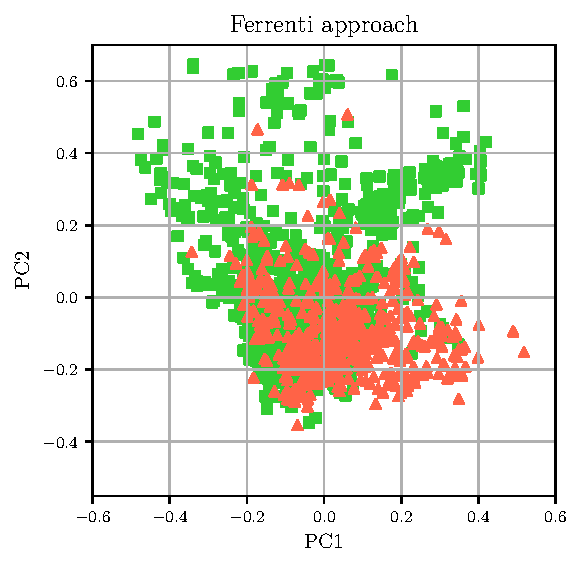
\includegraphics[width=1\textwidth]{figures/pca-2d-plots/01-ferrenti-approach-v3.pdf}
    \end{subfigure}%
    \begin{subfigure}{0.4\textwidth}
        \centering
        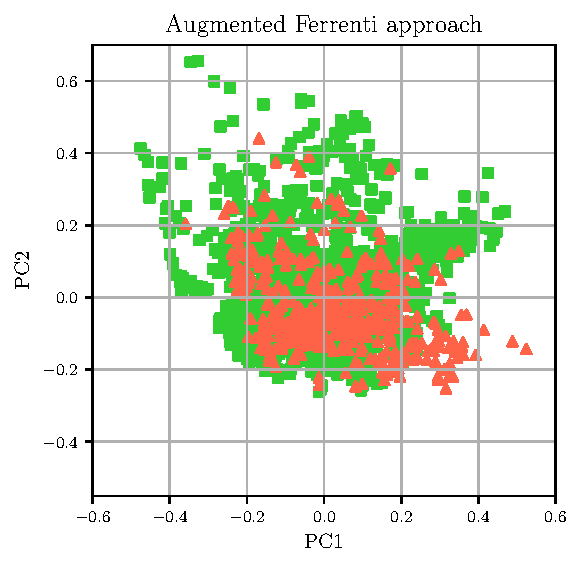
\includegraphics[width=1\textwidth]{figures/pca-2d-plots/02-augmented-ferrenti-approach-v2.pdf}
    \end{subfigure}
    
    \begin{subfigure}{0.5\textwidth}
        \centering
        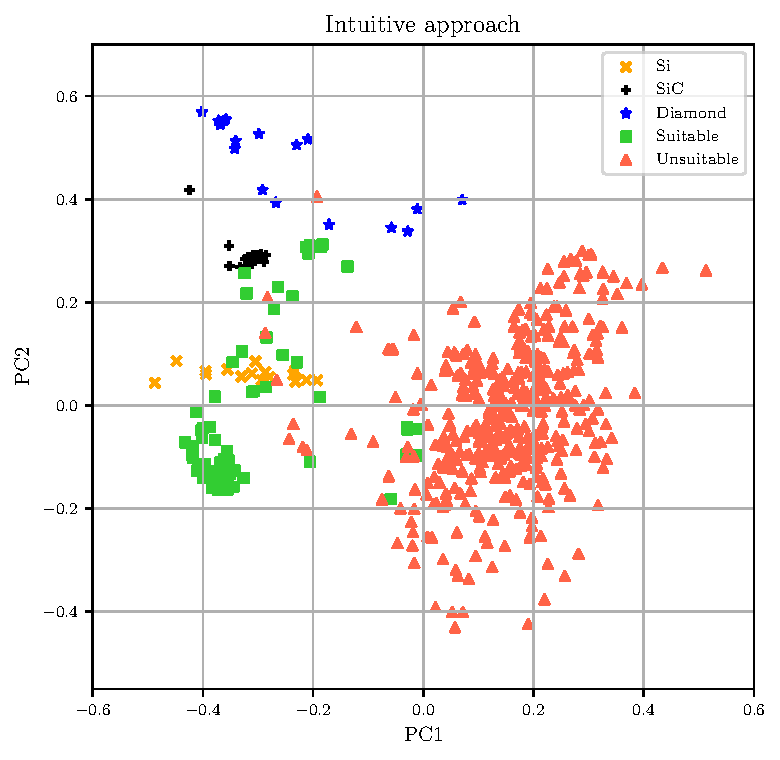
\includegraphics[width=1\textwidth]{figures/pca-2d-plots/03-insightful-approach-v3.pdf}
    \end{subfigure}
    %\vspace*{-95mm}
    \caption{Two-dimensional scatter plots for the three different approaches. We have identified the two eigenvectors corresponding to the two largest eigenvalues of the covariance-matrix, that is, the two most important principal components (PC1 and PC2) of the initial data from the Materials Project query. Then, we have transformed the three training sets resulting from the three approaches and visualized them as scatter plots. Green squares display suitable candidates and red triangles represent unsuitable candidates.}
    \label{fig:2dscatterplotpca}
\end{figure}

It seems likely that the differences in Fig.~\ref{fig:2dscatterplotpca} can be attributed to the specific choices made when extracting data in each of the three approaches. Where the intuitive approach takes advantage of the experimental knowledge that is available in the literature, the Ferrenti and augmented Ferrenti schemes rely on assumptions for which material properties are responsible for the desired quantum effects. An additional factor to consider is the use of practical considerations (e.g., toxic materials or the availability of spin zero isotopes) when restricting the parameter space for material choice. 
Intriguingly, a much clearer separation is observed for the intuitive approach, where no restrictions were imposed in terms of specific characteristics for the materials, as compared to the two others. 
These observations constitute an important finding of our work, as we show that it is possible to distinguish between suitable and unsuitable material candidates for QT. The manual approach for selecting suitable candidates based on experimental findings yields strong indications that a trend does exist and thus is possible to identify. This will be an important goal of a future work. 
Importantly, the methodology for selecting candidates as implemented in the intuitive approach can be adapted also to other material systems where a specific set of properties is desired (and observed or predicted for a sufficient number of materials) but the specific mechanisms behind them are unknown. 

%It is important to note that 
The constructed data sets encompass compounds formed by a plethora of combinations of surfaces, interfaces, nanostructures, compositions and structures. We note that this complexity is not necessarily reflected in the descriptors. 
Furthermore, we have utilized data obtained from high-throughput density functional theory calculations. Indeed, there are possible errors associated with every step, starting from an initial calculation, adding of data in the database, gathering of data, featurization of data, preprocessing of data, data mining, and finally training a model and making a prediction. Unfortunately, if an error has happened in the first part of the process, the error follows the entire process and will get increasingly harder to detect. Therefore, we are dependent on that the Materials Project database contains data with high quality, and we note that it is likely that there are some errors present in our data sets. 

Another potential source of uncertainty that should be mentioned is the use of the PBE functional for computing the information in the databases employed herein. Despite being immensely successful in describing a number of material properties, PBE is widely known for underestimating the band gap of semiconductors \cite{Freysoldt2014}. Therefore, not all properties predicted using the PBE functional are reliable, and the band gaps in particular cannot be trusted in absolute terms. Nonetheless, the functional is in wide use due to the combination of reasonable accuracy and high computational throughput, and is usually considered to be reliable for large-scale trends in semiconductor properties. 

In summary, using various data extraction tools for a number of materials science databases, we have obtained data sets consisting of over $25.000$ materials. The information from these data sets has then been converted into nearly $5000$ physics-informed features.  
After these steps with fine-tuning and selection of entries for our training sets we are now ready to apply machine learning methods on the test set in order to classify materials as potential candidates for quantum technology applications. 

\subsection*{Predicting Suitable Material Hosts for Quantum Technology} 
Four well-tested machine learning algorithms were employed in this work: logistic regression, decision trees, and ensemble methods like random forests and gradient boosting \cite{Mehta2019,Hastie2009}. 
These four machine learning methods were applied to the training sets that were optimized using each of the three approaches (Ferrenti, augmented Ferrenti and intuitive) outlined above. This yielded twelve sets of materials that were predicted as suitable material hosts for QT applications. In this section, we present representative results after applying machine learning methods to the training sets resulting from each of the three data mining approaches. 

%MB Here or further down? 
%I moved it up here from the Comparing the approaches section below, 
%because I moved the then Fig 5 (the predictions for each model and approach) into the Supplementary 
\begin{table}[b]
    \centering 
    \caption{Overview of the number of predicted suitable candidates as a function of ML model confidence when the four models in an approach agree. A cut-off value of $0.5$ represents the confidence of a coin flip, while $1.0$ is a fully confident prediction.}
    \begin{tabular}{c|c|c|c}
      & $0.50$ & $0.75$ & $0.85$ \\
     \hline
     Ferrenti approach &  $6804$ & $1784$ & $258$  \\
     Augmented Ferrenti approach &  $9227$ & $4735$  & $2001$  \\ 
     Intuitive approach & $214$ & $66$ & $9$ \\
     \hline
     All approaches together & $47$ & $6$ & 0 \\
    \end{tabular}
    \label{tab:probabilites}
\end{table} 

\subsubsection*{The Ferrenti approach}

We first consider the machine learning classification of the test set derived in the Ferrenti approach. The number of candidates predicted by each of the four machine learning methods 'Logistic regression', 'Decision trees', 'Random forests' and 'Gradient boosting' is contained in Figure~6 of the Supplementary Material at \cite{supplementary} for each of the three approaches. Table~\ref{tab:probabilites} contains an overview of the number of predicted suitable candidates as a function of ML model confidence when the four models in an approach agree. 

%MEB We can take this out, I suppose, if we need more space, and put it in Supplementary (I put fig 5 there) 
From the training set of $23.623$ materials, the four methods consistently predict at least $11.000$ materials as promising candidates in the case of the Ferrenti approach. All four ML methods agree on a total of $6804$ suitable candidates, however, many of these materials are predicted with an incidence similar to that of a coin flip. If we were to raise the minimum confidence cut-off of a prediction to (e.g.) $0.7$ instead of $0.5$, the above ML algorithms would only agree on $1784$ suitable candidates. 
We find that all four ML methods admit almost all materials with a chemical formula matching the known suitable candidates (see  Table~\ref{tab:qt-materials}) that were present in the training set. 
This can allow materials with unfortunate structures to be labeled as suitable candidates by all of our ML methods. 
%Be careful here - PBE is known for underestimating band gaps. 
For example, the ML methods do not perpetuate the band gap restriction from the training set definition. 
Based on the restrictions we defined initially, we would expect that all materials with band gaps lower than $0.5$~eV would be eliminated 
%for a cut-off set to above $0.5$ 
after applying the ML algorithms.  
Although this is expected behavior based on the training set, the trend is not carried over to the predicted data. We find that many entries with band gaps lower than $0.5$~eV are predicted as both suitable and unsuitable candidates by all four ML methods employed herein, 
indicating that the exact cut-off value we set for the band gap ($0.5$~eV for the Ferrenti approach) is not recognized by the machine learning algorithms. 
This cut-off value was imposed on the training data because small band gaps could make it challenging to facilitate deep level defects \cite{Weber2010}. 
On the other hand, due to the known underestimation of band gaps by the PBE functional, the band gaps could in reality be larger for many of the materials. 

\subsubsection*{The augmented Ferrenti approach}
Next, we turn to the more liberal augmented Ferrenti approach containing a $78 \ \%$ larger amount of materials than the former one. 
The four ML methods predict at least $13.000$ materials as suitable candidates out of $22.550$ materials in the training set, where they all agree on a total of $9227$ predicted suitable candidates. Comparing to the training set reveals that all of the unlabeled candidates that are known to be suitable (see Table~\ref{tab:qt-materials}) are, in fact, predicted as suitable candidates. Unfortunately, the ML methods also yield predictions that do not match with what one would expect from physical considerations. 
All four ML algorithms confidently (to probabilities of $83 \ \%$ and $60 \ \%$ for two different configurations) predict NaCl as a suitable candidate, which we believe is unlikely due to the strong electrostatic interactions between Na and Cl and the ionic character of their bonding (see, e.g., Ref.~\cite{Weber2010}).  
Indeed, single-photon emitters with sharp and bright zero-phonon lines are uncommon in materials with a strong ionic character. 
Moreover, despite enforcing an even more conservative band gap restriction of $1.5$~eV for the training set as compared to the Ferrenti approach, we still find that all four implemented ML methods predict suitable candidates that exhibit band gaps substantially lower than $0.5$~eV.
Clearly, the ML methods are not adhering rigidly to our imposed band gap restriction when classifying the materials. 
As we based this band gap restriction on assumptions for important material parameters in the QT context, the ML methods might be picking up on something we are not aware of. 
 
\subsubsection*{The intuitive approach}
The ML methods that were trained on the data extracted in the intuitive approach predict substantially fewer candidates as compared to the other two approaches. 
A total of $842$, $1197$, $543$ and $596$ materials are classified as suitable candidates by logistic regression, decision trees, random forests and gradient boosting, respectively. All the four ML methods agree on a total of $214$ suitable candidates for a $0.5$ cut-off restriction.  
Although this is comparable to the probability of a coin toss, the agreement of the four ML algorithms lends support to the suitability of the $214$ materials. 
Note that $51$ of these have a band gap of $0.5$~eV or smaller as reported in Materials Project from PBE-level DFT calculations.   

%Cut down the amount of information given on perhaps not so suitable candidates, while rather emphasize the good predicted suitable candidates?

Initially, we consider the materials that were classified as suitable to a confidence of $0.85$ or higher by all four ML models; BN, CdSe, BC$_2$N, InAs, CuI, and ZnCd$_3$Se$_4$. 
The compound BN (mp-$1639$) was in fact present in the training data as a suitable candidate, we believe this is a reason why the models recognize BN  as a suitable candidate with high probability. Furthermore, two compositions of CdSe (the cubic mp-$2691$ and the hexagonal mp-$1070$) have been predicted as suitable, possibly as a consequence of the similar compound CdS being labeled as a suitable candidate in the training set. 
%The element S resides in the same group as Se, and 
The two compounds of CdSe share similar properties with calculated band gaps of $0.5$~eV and $0.6$~eV, respectively, in the MP database.  
Comparing to experiment, ... 
%high quality nanocrystals of CdS have been synthesized and studied for use as quantum dots since the nanocrystals emit in the visible range with a direct band gap of $2.5$-$2.6$~eV \cite{BanerjeeR2000Eots,CelebiSerdar2007SaCo,Qutub2012}. 
%Bulk CdS has a slightly lower reported band gap of $2.4$~eV \cite{Qutub2012}.  

In the case of BC$_2$N we find two compositions with the same chemical formula; the orthorhombically coordinated (mp-$629458$) and the chalcopyrite structured (mp-$1008523$) BC$_2$N. The former takes on a polar space group while the latter does not. The band gaps are listed as $1.9$~eV and $1.7$~eV, respectively, in the MP database. 
%BC$_2$N is known as heterodiamond and is a hybrid of diamond and BN. 
Both structures exhibit, as expected, strong covalent character and have been studied for applications as nanostructures for electronic devices \cite{Gao2017}, hydrogen storage \cite{Cai2017} and superhard materials \cite{Li2017, Jiang2020}. It has similarly been predicted that the diamond-like structure of BC$_3$N can be a prominent spin qubit material host \cite{Wang2020SpinQB}. By creating a boron (B) vacancy one can in theory obtain a defect center with similar properties to those found for the NV center in diamond. Whether this is also possible for BC$_2$N remains to be seen. We note that BC$_3$N was not represented in the MP database at the time of downloading and is therefore not included in our dataset. 

The compounds InAs (cubic, mp-$20305$), CuI (cubic, mp-$22895$ and hexagonal, mp-$569346$) and ZnCd$_3$Se$_4$ (cubic, mp-$1078597$) are listed in the MP database with band gaps of $0.3$, $1.2$ and $1.7$~eV, respectively. 
%, and exhibit comparable properties. 
To the best of our knowledge, ZnCd$_3$Se$_4$ has yet to be synthesized. 
Self-assembled InAs quantum dots are an exciting possible material to use in quantum technology \cite{Liu2018}. 
CuI has recently been synthesized as single-crystal epitaxial films and was shown to exhibit remarkable optoelectronic properties \cite{Ahn2020}.  Interestingly, the material exhibits a large ionic character with more similarities to some of the oxide compounds in the data set than, e.g., the materials that are more covalent in character like Si, SiC and  diamond.  
It seems that ionic character alone is not an obstacle for a material to be quantum compatible if the prediction of CuI proves to be merited. It is unknown at this time whether any potential quantum compatible properties of CuI would originate from deep level defects or nanostructuring (e.g., quantum dots). Note that NaCl was not predicted as suitable for QT in the intuitive approach.  
%and contains the toxic element Cd, which could prove an obstacle for large scale utilization. 

Lowering the cut-off requirement from $0.85$ to $0.75$ for all models results in $66$ candidate materials. 
The full list of these $66$ is contained in the Supplementary Material at \cite{supplementary}. 
The list of predicted suitable candidates now also includes ternary compounds of the formula ABC$_2$, in addition to elemental and binary semiconductors, and the nine materials listed above. For the ABC$_2$ structures, the elements Ga, Cd, In and Zn can occupy the A-site, Cu, Sn, Ag and Ge take the B-site, while S, Se, Te, P or As may reside at the C site. Most of the predicted compounds include at least one toxic element with one exception: ZnGeP$_2$ (mp-$4524$) in a chalcopyrite-like structure with an indirect band gap of $1.2$~eV \cite{Zhang2015} as reported in the MP database. In comparison, the experimentally reported band gap is somewhat larger at $2.0$~eV \cite{Xing1989}. 
ZnGeP$_2$ crystallizes in a non-polar space group, possesses no magnetic moment, exhibits strongly covalent bonds, and has been reported as an excellent mid-IR transparent crystal material that is suitable for nonlinear optical applications \cite{Zhang2015}. Importantly, it is possible to integrate sources of photon quantum states based on nonlinear optics with ZnGeP$_2$ \cite{Caspani2017}. 
We therefore identify ZnGeP$_2$ as an eligible candidate material for QT, but it remains to be seen whether the candidate can facilitate, e.g., the isolated deep energy levels often associated with defects exhibiting quantum compatible properties, or perhaps be a candidate for nanostructure based QT.  

Among the $66$ materials that all models in the intuitive approach agreed on to a $0.75$ confidence level, we emphasize the presence of interesting materials like Ge (in three configurations mp-$137$, mp-$1067619$ and mp-$1198022$), GeC, BP and InP. Ge in the cubic structure (mp-$1198022$) shares many properties with Si and C in addition to the periodic column number. 
Ge has the highest hole mobility of all semiconductors at room temperature, and is therefore considered a key material for the process of extending the chip performance in classical computers beyond the limits imposed by miniaturization \cite{Scappucci2020}. Furthermore, like SiC, device design based on Ge can take advantage of the mature large-scale fabrication of silicon due to the material's comparable properties.  
Similar considerations could be made for the case of GeC. 
Data from the Materials Project database suggests that the cubic compound GeC (mp-$1002164$) is a covalently bonded semiconductor having a band gap of $1.8$~eV. 
Consequently, as SiC is widely known as a highly suitable host material for QT compatible defects, we encourage further research on GeC due to its similarities to SiC. 

The compound BP (mp-$1479$ and mp-$1008559$) is present in our predictions in both the cubic and hexagonal structures. The indirect band gaps of the different structures are calculated at $1.5$~eV and $1.1$~eV, respectively, as reported in the MP database. Both configurations of BP are nonmagnetic and share several properties with the entries mentioned above; including ... BP is non-toxic and has been synthesized with a potential for large-scale production \cite{MukhanovVladimirA2016Umso}.

Lastly, we will discuss the prediction of InP (mp-$966800$) as a suitable candidate. The compound inhabits the hexagonal structure with corner-sharing InP$_4$ tetrahedra. InP is reported in the Materials Project to have a direct band gap of $0.5$~eV and is considered as one of the most promising candidates to compete with Cd- or Pb- based QDs for, e.g., display and lighting applications  \cite{Zhang2020a, Won2019}. 
We underline the possibility of using InP-based quantum dots for QT applications as well.  

It is worth mentioning that all models agree on several oxides being potential candidates when the prediction cut-off is set low enough (but still above $0.5$). However, we find that almost all the oxide compounds fall between the decision boundary defining suitable and unsuitable candidates, and none are present in the list containing the $66$ suitable candidates ($0.75$ cut-off) in the Supplementary Material. Due to the labeling of ZnO as a suitable candidate, we believe that the boundary was shifted sufficiently to admit several oxides as suitable candidates. 
Removing ZnO from the training set for the intuitive approach might result in fewer or even no oxide compounds being predicted above a suitability limit of $0.5$ and could be an interesting future pathway for investigation. 

In comparison, the work of \citeauthor{Ferrenti2020} \cite{Ferrenti2020} suggests a list of $541$ viable hosts after the data mining procedure.  
Among these these, we find only a single material present in our list of $66$ candidates predicted by the four ML models after training on the dataset resulting from the intuitive approach. This material is the nontoxic compound MgSe (mp-$10760$) which crystallizes in the rock-salt structure. Its band gap is $2.0$~eV in the MP database with the experimental value being reported from $2.45$~eV (optical band gap) \cite{Ubale2014} up to as large as $5.6$~eV \cite{SaumGeorge1959}. MgSe is notable for its available spin-zero isotopes in accordance with the criteria set by \citeauthor{Weber2010} \cite{Weber2010} and \citeauthor{Ferrenti2020} Ref.~\cite{Ferrenti2020}. We believe that these criteria may favor defects acting as spin centers with qubit potential and MgSe is thus identified as a promising host material in this respect.   
%\oliver{Maybe also see if other compounds that were present in training set are present in their 541 hosts. }

\begin{figure}%[h] %!tbp
    \centering
    \begin{subfigure}{1\textwidth}
        \centering
        %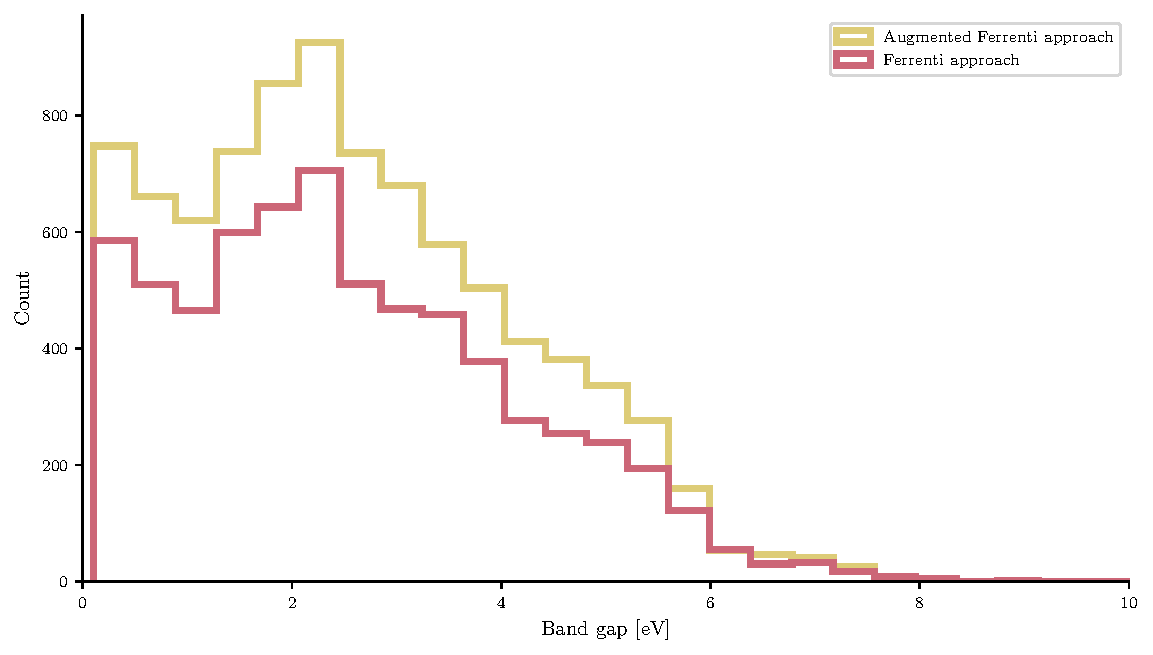
\includegraphics[width=1\textwidth]{figures/histograms/01-02-histogram-.pdf}
        % This file was created with tikzplotlib v0.9.16.
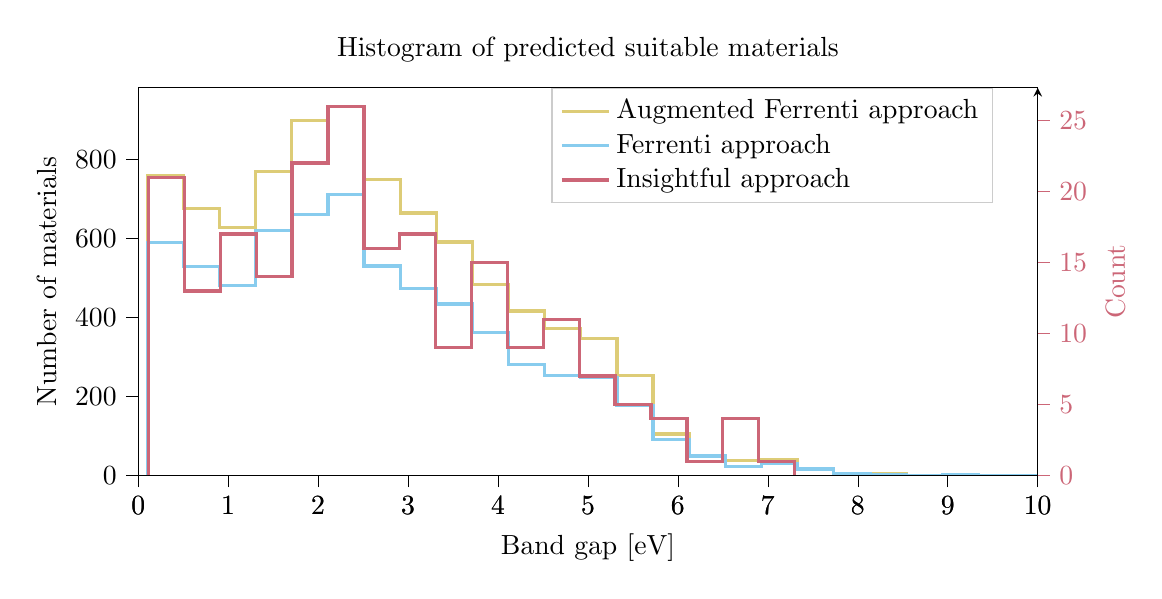
\begin{tikzpicture}

\definecolor{color0}{rgb}{0.866666666666667,0.8,0.466666666666667}
\definecolor{color1}{rgb}{0.533333333333333,0.8,0.933333333333333}
\definecolor{color2}{rgb}{0.8,0.4,0.466666666666667}

\begin{axis}[
height=2.5600388542963888in,
legend cell align={left},
legend style={fill opacity=0.8, draw opacity=1, text opacity=1, draw=white!80!black, at={(0.95,1)}},
tick align=outside,
tick pos=left,
title={Histogram of predicted suitable materials},
width=5.1200777085927776in,
x grid style={white!69.0196078431373!black},
xlabel={Band gap [eV]},
xmin=0, xmax=10,
xtick style={color=black},
y grid style={white!69.0196078431373!black},
ylabel={Number of materials},
ymin=0, ymax=980.7,
ytick style={color=black}
]
\path [draw=color0, very thick]
(axis cs:0.1003,0)
--(axis cs:0.1003,759)
--(axis cs:0.502006818181818,759)
--(axis cs:0.502006818181818,675)
--(axis cs:0.903713636363636,675)
--(axis cs:0.903713636363636,628)
--(axis cs:1.30542045454545,628)
--(axis cs:1.30542045454545,769)
--(axis cs:1.70712727272727,769)
--(axis cs:1.70712727272727,898)
--(axis cs:2.10883409090909,898)
--(axis cs:2.10883409090909,934)
--(axis cs:2.51054090909091,934)
--(axis cs:2.51054090909091,748)
--(axis cs:2.91224772727273,748)
--(axis cs:2.91224772727273,664)
--(axis cs:3.31395454545454,664)
--(axis cs:3.31395454545454,591)
--(axis cs:3.71566136363636,591)
--(axis cs:3.71566136363636,483)
--(axis cs:4.11736818181818,483)
--(axis cs:4.11736818181818,416)
--(axis cs:4.519075,416)
--(axis cs:4.519075,371)
--(axis cs:4.92078181818182,371)
--(axis cs:4.92078181818182,347)
--(axis cs:5.32248863636364,347)
--(axis cs:5.32248863636364,253)
--(axis cs:5.72419545454545,253)
--(axis cs:5.72419545454545,105)
--(axis cs:6.12590227272727,105)
--(axis cs:6.12590227272727,49)
--(axis cs:6.52760909090909,49)
--(axis cs:6.52760909090909,38)
--(axis cs:6.92931590909091,38)
--(axis cs:6.92931590909091,40)
--(axis cs:7.33102272727273,40)
--(axis cs:7.33102272727273,16)
--(axis cs:7.73272954545454,16)
--(axis cs:7.73272954545454,3)
--(axis cs:8.13443636363636,3)
--(axis cs:8.13443636363636,4)
--(axis cs:8.53614318181818,4)
--(axis cs:8.53614318181818,0)
--(axis cs:8.93785,0)
--(axis cs:8.93785,1)
--(axis cs:9.33955681818182,1)
--(axis cs:9.33955681818182,0)
--(axis cs:9.74126363636364,0)
--(axis cs:9.74126363636364,0)
--(axis cs:10.1429704545455,0)
--(axis cs:10.1429704545455,0)
--(axis cs:10.5446772727273,0)
--(axis cs:10.5446772727273,0)
--(axis cs:10.9463840909091,0)
--(axis cs:10.9463840909091,0)
--(axis cs:11.3480909090909,0)
--(axis cs:11.3480909090909,0)
--(axis cs:11.7497977272727,0)
--(axis cs:11.7497977272727,0)
--(axis cs:12.1515045454545,0)
--(axis cs:12.1515045454545,0)
--(axis cs:12.5532113636364,0)
--(axis cs:12.5532113636364,0)
--(axis cs:12.9549181818182,0)
--(axis cs:12.9549181818182,0)
--(axis cs:13.356625,0)
--(axis cs:13.356625,0)
--(axis cs:13.7583318181818,0)
--(axis cs:13.7583318181818,0)
--(axis cs:14.1600386363636,0)
--(axis cs:14.1600386363636,0)
--(axis cs:14.5617454545455,0)
--(axis cs:14.5617454545455,0)
--(axis cs:14.9634522727273,0)
--(axis cs:14.9634522727273,0)
--(axis cs:15.3651590909091,0)
--(axis cs:15.3651590909091,0)
--(axis cs:15.7668659090909,0)
--(axis cs:15.7668659090909,0)
--(axis cs:16.1685727272727,0)
--(axis cs:16.1685727272727,0)
--(axis cs:16.5702795454545,0)
--(axis cs:16.5702795454545,0)
--(axis cs:16.9719863636364,0)
--(axis cs:16.9719863636364,0)
--(axis cs:17.3736931818182,0)
--(axis cs:17.3736931818182,1)
--(axis cs:17.7754,1)
--(axis cs:17.7754,0);
\addlegendimage{line legend, draw=color0, very thick}
\addlegendentry{Augmented Ferrenti approach}

\path [draw=color1, very thick]
(axis cs:0.1003,0)
--(axis cs:0.1003,589)
--(axis cs:0.502006818181818,589)
--(axis cs:0.502006818181818,528)
--(axis cs:0.903713636363636,528)
--(axis cs:0.903713636363636,480)
--(axis cs:1.30542045454545,480)
--(axis cs:1.30542045454545,619)
--(axis cs:1.70712727272727,619)
--(axis cs:1.70712727272727,660)
--(axis cs:2.10883409090909,660)
--(axis cs:2.10883409090909,711)
--(axis cs:2.51054090909091,711)
--(axis cs:2.51054090909091,530)
--(axis cs:2.91224772727273,530)
--(axis cs:2.91224772727273,473)
--(axis cs:3.31395454545454,473)
--(axis cs:3.31395454545454,434)
--(axis cs:3.71566136363636,434)
--(axis cs:3.71566136363636,361)
--(axis cs:4.11736818181818,361)
--(axis cs:4.11736818181818,281)
--(axis cs:4.519075,281)
--(axis cs:4.519075,252)
--(axis cs:4.92078181818182,252)
--(axis cs:4.92078181818182,247)
--(axis cs:5.32248863636364,247)
--(axis cs:5.32248863636364,177)
--(axis cs:5.72419545454545,177)
--(axis cs:5.72419545454545,90)
--(axis cs:6.12590227272727,90)
--(axis cs:6.12590227272727,49)
--(axis cs:6.52760909090909,49)
--(axis cs:6.52760909090909,23)
--(axis cs:6.92931590909091,23)
--(axis cs:6.92931590909091,30)
--(axis cs:7.33102272727273,30)
--(axis cs:7.33102272727273,16)
--(axis cs:7.73272954545454,16)
--(axis cs:7.73272954545454,5)
--(axis cs:8.13443636363636,5)
--(axis cs:8.13443636363636,3)
--(axis cs:8.53614318181818,3)
--(axis cs:8.53614318181818,0)
--(axis cs:8.93785,0)
--(axis cs:8.93785,1)
--(axis cs:9.33955681818182,1)
--(axis cs:9.33955681818182,0)
--(axis cs:9.74126363636364,0)
--(axis cs:9.74126363636364,0)
--(axis cs:10.1429704545455,0)
--(axis cs:10.1429704545455,0)
--(axis cs:10.5446772727273,0)
--(axis cs:10.5446772727273,0)
--(axis cs:10.9463840909091,0)
--(axis cs:10.9463840909091,0)
--(axis cs:11.3480909090909,0)
--(axis cs:11.3480909090909,0)
--(axis cs:11.7497977272727,0)
--(axis cs:11.7497977272727,0)
--(axis cs:12.1515045454545,0)
--(axis cs:12.1515045454545,0)
--(axis cs:12.5532113636364,0)
--(axis cs:12.5532113636364,0)
--(axis cs:12.9549181818182,0)
--(axis cs:12.9549181818182,0)
--(axis cs:13.356625,0)
--(axis cs:13.356625,0)
--(axis cs:13.7583318181818,0)
--(axis cs:13.7583318181818,0)
--(axis cs:14.1600386363636,0)
--(axis cs:14.1600386363636,0)
--(axis cs:14.5617454545455,0)
--(axis cs:14.5617454545455,0)
--(axis cs:14.9634522727273,0)
--(axis cs:14.9634522727273,0)
--(axis cs:15.3651590909091,0)
--(axis cs:15.3651590909091,0)
--(axis cs:15.7668659090909,0)
--(axis cs:15.7668659090909,0)
--(axis cs:16.1685727272727,0)
--(axis cs:16.1685727272727,0)
--(axis cs:16.5702795454545,0)
--(axis cs:16.5702795454545,0)
--(axis cs:16.9719863636364,0)
--(axis cs:16.9719863636364,0)
--(axis cs:17.3736931818182,0)
--(axis cs:17.3736931818182,1)
--(axis cs:17.7754,1)
--(axis cs:17.7754,0);
\addlegendimage{line legend, draw=color1, very thick}
\addlegendentry{Ferrenti approach}

\addlegendimage{line legend, draw=color2, very thick}
\addlegendentry{Insightful approach}
\end{axis}

\begin{axis}[
axis y line=right,
height=2.5600388542963888in,
tick align=outside,
width=5.1200777085927776in,
x grid style={white!69.0196078431373!black},
xmin=0, xmax=10,
xtick pos=left,
xtick style={color=black},
y grid style={white!69.0196078431373!black},
ylabel=\textcolor{color2}{Count},
ymin=0, ymax=27.3,
ytick pos=right,
ytick style={color=color2},
yticklabel style={anchor=west, color=color2}
]
\path [draw=color2, very thick]
(axis cs:0.1157,0)
--(axis cs:0.1157,21)
--(axis cs:0.514638888888889,21)
--(axis cs:0.514638888888889,13)
--(axis cs:0.913577777777778,13)
--(axis cs:0.913577777777778,17)
--(axis cs:1.31251666666667,17)
--(axis cs:1.31251666666667,14)
--(axis cs:1.71145555555556,14)
--(axis cs:1.71145555555556,22)
--(axis cs:2.11039444444444,22)
--(axis cs:2.11039444444444,26)
--(axis cs:2.50933333333333,26)
--(axis cs:2.50933333333333,16)
--(axis cs:2.90827222222222,16)
--(axis cs:2.90827222222222,17)
--(axis cs:3.30721111111111,17)
--(axis cs:3.30721111111111,9)
--(axis cs:3.70615,9)
--(axis cs:3.70615,15)
--(axis cs:4.10508888888889,15)
--(axis cs:4.10508888888889,9)
--(axis cs:4.50402777777778,9)
--(axis cs:4.50402777777778,11)
--(axis cs:4.90296666666667,11)
--(axis cs:4.90296666666667,7)
--(axis cs:5.30190555555555,7)
--(axis cs:5.30190555555555,5)
--(axis cs:5.70084444444444,5)
--(axis cs:5.70084444444444,4)
--(axis cs:6.09978333333333,4)
--(axis cs:6.09978333333333,1)
--(axis cs:6.49872222222222,1)
--(axis cs:6.49872222222222,4)
--(axis cs:6.89766111111111,4)
--(axis cs:6.89766111111111,1)
--(axis cs:7.2966,1)
--(axis cs:7.2966,0);
\end{axis}

\end{tikzpicture}

        \subcaption[]{}
    \end{subfigure}%

    
    \begin{subfigure}{1\textwidth}
        \centering
        %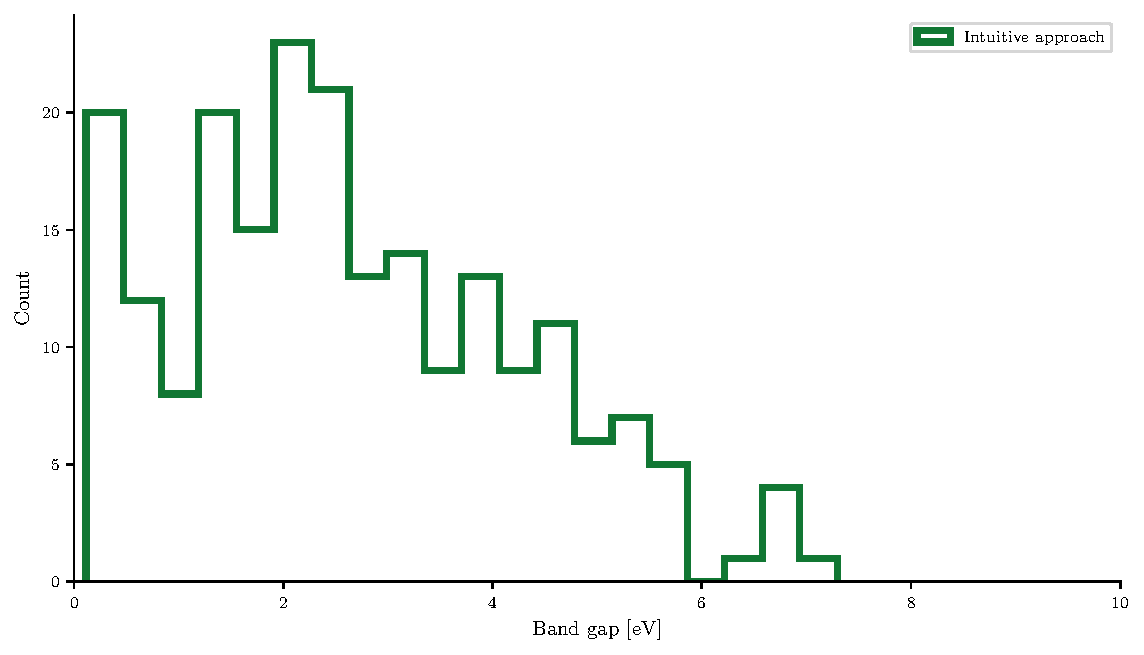
\includegraphics[width=1\textwidth]{figures/histograms/03-histogram-.pdf}
        % This file was created with tikzplotlib v0.9.16.
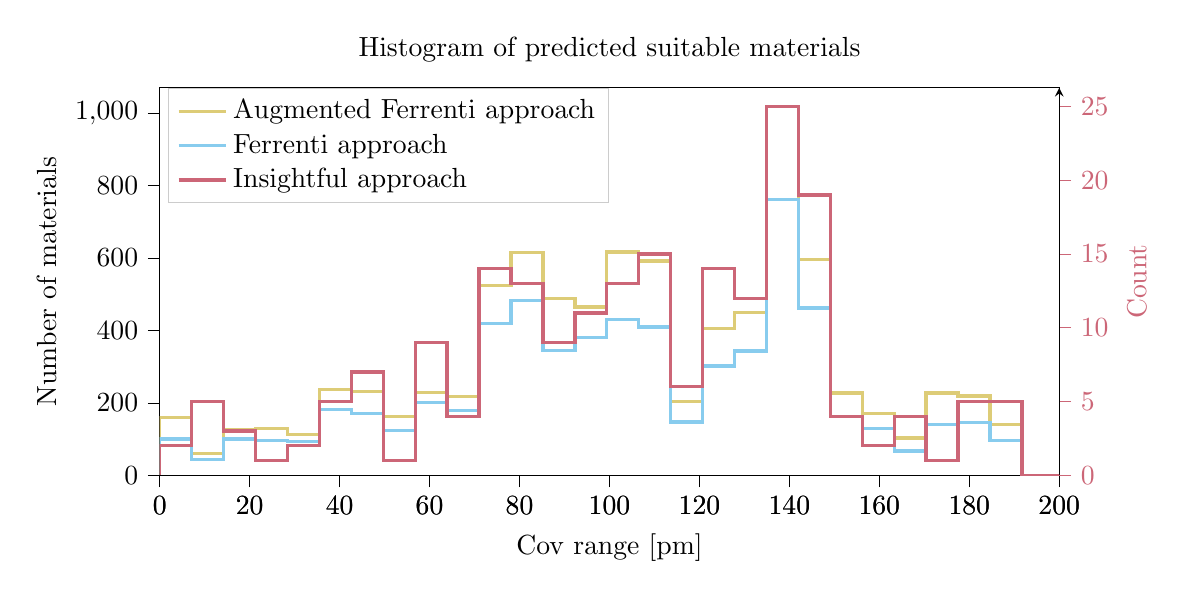
\begin{tikzpicture}

\definecolor{color0}{rgb}{0.866666666666667,0.8,0.466666666666667}
\definecolor{color1}{rgb}{0.533333333333333,0.8,0.933333333333333}
\definecolor{color2}{rgb}{0.8,0.4,0.466666666666667}

\begin{axis}[
height=2.5600388542963888in,
legend cell align={left},
legend style={fill opacity=0.8, draw opacity=1, text opacity=1, draw=white!80!black, at={(0.5,1)}},
tick align=outside,
tick pos=left,
title={Histogram of predicted suitable materials},
width=5.1200777085927776in,
x grid style={white!69.0196078431373!black},
xlabel={Cov range [pm]},
xmin=0, xmax=200,
xtick style={color=black},
y grid style={white!69.0196078431373!black},
ylabel={Number of materials},
ymin=0, ymax=1069.95,
ytick style={color=black}
]
\path [draw=color0, very thick]
(axis cs:0,0)
--(axis cs:0,160)
--(axis cs:7.1,160)
--(axis cs:7.1,61)
--(axis cs:14.2,61)
--(axis cs:14.2,127)
--(axis cs:21.3,127)
--(axis cs:21.3,129)
--(axis cs:28.4,129)
--(axis cs:28.4,112)
--(axis cs:35.5,112)
--(axis cs:35.5,237)
--(axis cs:42.6,237)
--(axis cs:42.6,231)
--(axis cs:49.7,231)
--(axis cs:49.7,162)
--(axis cs:56.8,162)
--(axis cs:56.8,229)
--(axis cs:63.9,229)
--(axis cs:63.9,217)
--(axis cs:71,217)
--(axis cs:71,525)
--(axis cs:78.1,525)
--(axis cs:78.1,615)
--(axis cs:85.2,615)
--(axis cs:85.2,488)
--(axis cs:92.3,488)
--(axis cs:92.3,465)
--(axis cs:99.4,465)
--(axis cs:99.4,617)
--(axis cs:106.5,617)
--(axis cs:106.5,592)
--(axis cs:113.6,592)
--(axis cs:113.6,203)
--(axis cs:120.7,203)
--(axis cs:120.7,406)
--(axis cs:127.8,406)
--(axis cs:127.8,449)
--(axis cs:134.9,449)
--(axis cs:134.9,1019)
--(axis cs:142,1019)
--(axis cs:142,596)
--(axis cs:149.1,596)
--(axis cs:149.1,227)
--(axis cs:156.2,227)
--(axis cs:156.2,171)
--(axis cs:163.3,171)
--(axis cs:163.3,103)
--(axis cs:170.4,103)
--(axis cs:170.4,227)
--(axis cs:177.5,227)
--(axis cs:177.5,219)
--(axis cs:184.6,219)
--(axis cs:184.6,141)
--(axis cs:191.7,141)
--(axis cs:191.7,0)
--(axis cs:198.8,0)
--(axis cs:198.8,0)
--(axis cs:205.9,0)
--(axis cs:205.9,65)
--(axis cs:213,65)
--(axis cs:213,0);
\addlegendimage{line legend, draw=color0, very thick}
\addlegendentry{Augmented Ferrenti approach}

\path [draw=color1, very thick]
(axis cs:0,0)
--(axis cs:0,100)
--(axis cs:7.1,100)
--(axis cs:7.1,44)
--(axis cs:14.2,44)
--(axis cs:14.2,100)
--(axis cs:21.3,100)
--(axis cs:21.3,97)
--(axis cs:28.4,97)
--(axis cs:28.4,94)
--(axis cs:35.5,94)
--(axis cs:35.5,181)
--(axis cs:42.6,181)
--(axis cs:42.6,170)
--(axis cs:49.7,170)
--(axis cs:49.7,124)
--(axis cs:56.8,124)
--(axis cs:56.8,202)
--(axis cs:63.9,202)
--(axis cs:63.9,180)
--(axis cs:71,180)
--(axis cs:71,419)
--(axis cs:78.1,419)
--(axis cs:78.1,482)
--(axis cs:85.2,482)
--(axis cs:85.2,345)
--(axis cs:92.3,345)
--(axis cs:92.3,380)
--(axis cs:99.4,380)
--(axis cs:99.4,430)
--(axis cs:106.5,430)
--(axis cs:106.5,410)
--(axis cs:113.6,410)
--(axis cs:113.6,147)
--(axis cs:120.7,147)
--(axis cs:120.7,302)
--(axis cs:127.8,302)
--(axis cs:127.8,343)
--(axis cs:134.9,343)
--(axis cs:134.9,762)
--(axis cs:142,762)
--(axis cs:142,462)
--(axis cs:149.1,462)
--(axis cs:149.1,162)
--(axis cs:156.2,162)
--(axis cs:156.2,129)
--(axis cs:163.3,129)
--(axis cs:163.3,67)
--(axis cs:170.4,67)
--(axis cs:170.4,141)
--(axis cs:177.5,141)
--(axis cs:177.5,146)
--(axis cs:184.6,146)
--(axis cs:184.6,97)
--(axis cs:191.7,97)
--(axis cs:191.7,0)
--(axis cs:198.8,0)
--(axis cs:198.8,0)
--(axis cs:205.9,0)
--(axis cs:205.9,44)
--(axis cs:213,44)
--(axis cs:213,0);
\addlegendimage{line legend, draw=color1, very thick}
\addlegendentry{Ferrenti approach}

\addlegendimage{line legend, draw=color2, very thick}
\addlegendentry{Insightful approach}

\end{axis}

\begin{axis}[
axis y line=right,
height=2.5600388542963888in,
tick align=outside,
width=5.1200777085927776in,
x grid style={white!69.0196078431373!black},
xmin=0, xmax=200,
xtick pos=left,
xtick style={color=black},
y grid style={white!69.0196078431373!black},
ylabel=\textcolor{color2}{Count},
ymin=0, ymax=26.25,
ytick pos=right,
ytick style={color=color2},
yticklabel style={anchor=west, color=color2}
]
\path [draw=color2, very thick]
(axis cs:0,0)
--(axis cs:0,2)
--(axis cs:7.1,2)
--(axis cs:7.1,5)
--(axis cs:14.2,5)
--(axis cs:14.2,3)
--(axis cs:21.3,3)
--(axis cs:21.3,1)
--(axis cs:28.4,1)
--(axis cs:28.4,2)
--(axis cs:35.5,2)
--(axis cs:35.5,5)
--(axis cs:42.6,5)
--(axis cs:42.6,7)
--(axis cs:49.7,7)
--(axis cs:49.7,1)
--(axis cs:56.8,1)
--(axis cs:56.8,9)
--(axis cs:63.9,9)
--(axis cs:63.9,4)
--(axis cs:71,4)
--(axis cs:71,14)
--(axis cs:78.1,14)
--(axis cs:78.1,13)
--(axis cs:85.2,13)
--(axis cs:85.2,9)
--(axis cs:92.3,9)
--(axis cs:92.3,11)
--(axis cs:99.4,11)
--(axis cs:99.4,13)
--(axis cs:106.5,13)
--(axis cs:106.5,15)
--(axis cs:113.6,15)
--(axis cs:113.6,6)
--(axis cs:120.7,6)
--(axis cs:120.7,14)
--(axis cs:127.8,14)
--(axis cs:127.8,12)
--(axis cs:134.9,12)
--(axis cs:134.9,25)
--(axis cs:142,25)
--(axis cs:142,19)
--(axis cs:149.1,19)
--(axis cs:149.1,4)
--(axis cs:156.2,4)
--(axis cs:156.2,2)
--(axis cs:163.3,2)
--(axis cs:163.3,4)
--(axis cs:170.4,4)
--(axis cs:170.4,1)
--(axis cs:177.5,1)
--(axis cs:177.5,5)
--(axis cs:184.6,5)
--(axis cs:184.6,5)
--(axis cs:191.7,5)
--(axis cs:191.7,0)
--(axis cs:198.8,0)
--(axis cs:198.8,0)
--(axis cs:205.9,0)
--(axis cs:205.9,1)
--(axis cs:213,1)
--(axis cs:213,0);
\end{axis}

\end{tikzpicture}

        \subcaption[]{}
    \end{subfigure}

    \begin{subfigure}{1\textwidth}
        \centering
        %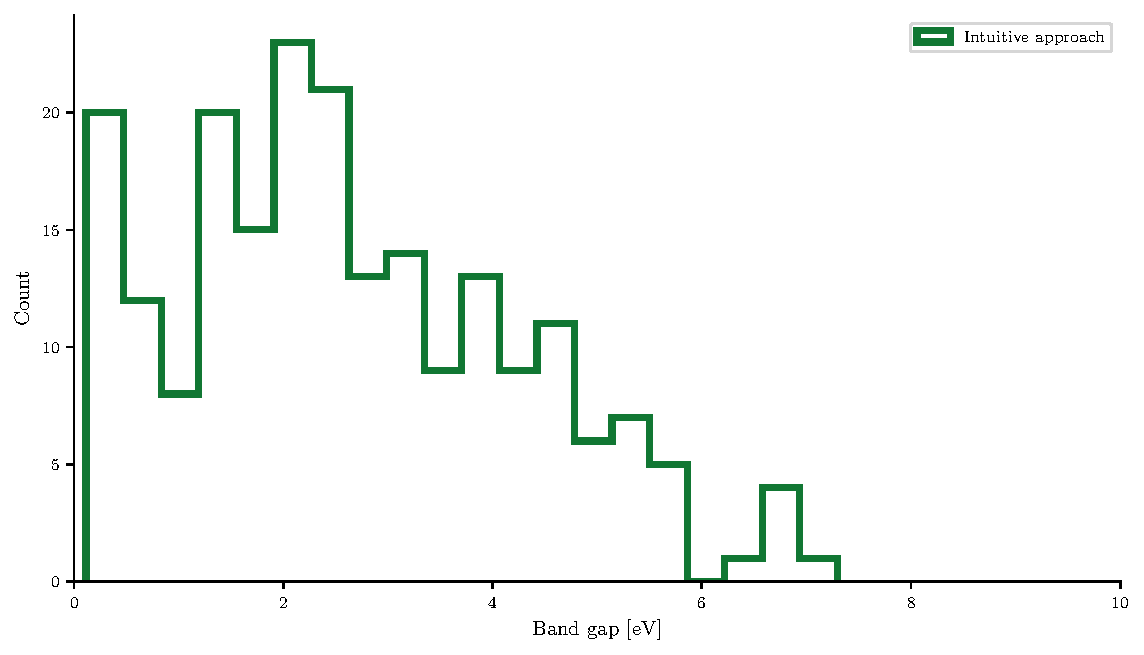
\includegraphics[width=1\textwidth]{figures/histograms/03-histogram-.pdf}
        % This file was created with tikzplotlib v0.9.16.
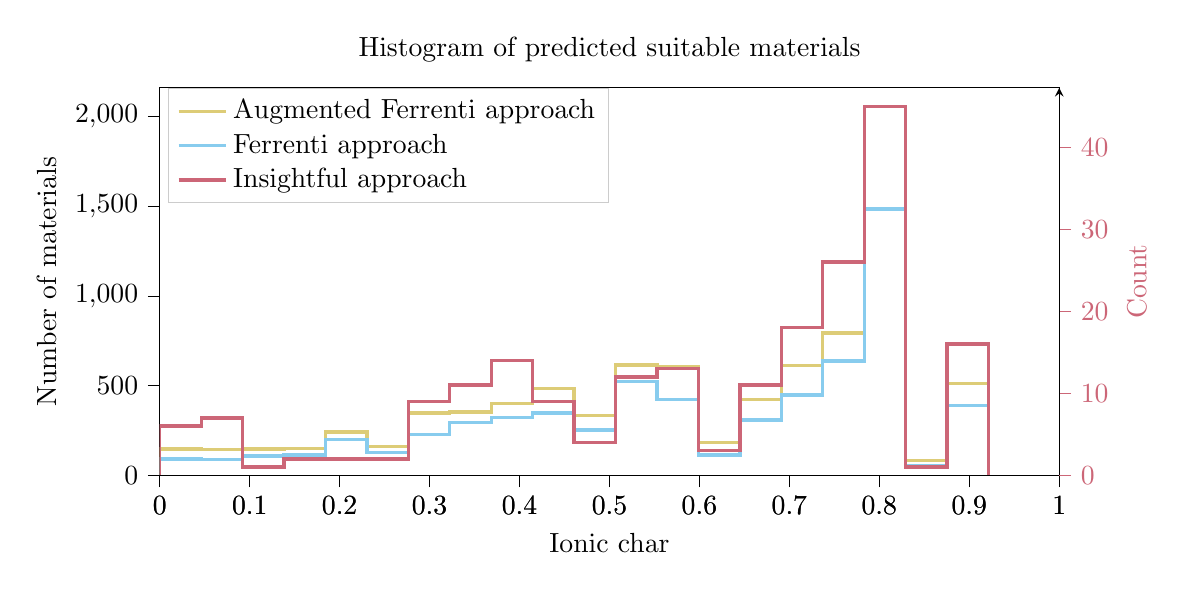
\begin{tikzpicture}

\definecolor{color0}{rgb}{0.866666666666667,0.8,0.466666666666667}
\definecolor{color1}{rgb}{0.533333333333333,0.8,0.933333333333333}
\definecolor{color2}{rgb}{0.8,0.4,0.466666666666667}

\begin{axis}[
height=2.5600388542963888in,
legend cell align={left},
legend style={fill opacity=0.8, draw opacity=1, text opacity=1, draw=white!80!black, at={(0.5,1)}},
tick align=outside,
tick pos=left,
title={Histogram of predicted suitable materials},
width=5.1200777085927776in,
x grid style={white!69.0196078431373!black},
xlabel={Ionic char},
xmin=0, xmax=1,
xtick style={color=black},
y grid style={white!69.0196078431373!black},
ylabel={Number of materials},
ymin=0, ymax=2158.8,
ytick style={color=black}
]
\path [draw=color0, very thick]
(axis cs:0,0)
--(axis cs:0,147)
--(axis cs:0.0460725199741125,147)
--(axis cs:0.0460725199741125,143)
--(axis cs:0.092145039948225,143)
--(axis cs:0.092145039948225,146)
--(axis cs:0.138217559922338,146)
--(axis cs:0.138217559922338,148)
--(axis cs:0.18429007989645,148)
--(axis cs:0.18429007989645,241)
--(axis cs:0.230362599870563,241)
--(axis cs:0.230362599870563,162)
--(axis cs:0.276435119844675,162)
--(axis cs:0.276435119844675,347)
--(axis cs:0.322507639818788,347)
--(axis cs:0.322507639818788,353)
--(axis cs:0.3685801597929,353)
--(axis cs:0.3685801597929,402)
--(axis cs:0.414652679767013,402)
--(axis cs:0.414652679767013,484)
--(axis cs:0.460725199741125,484)
--(axis cs:0.460725199741125,332)
--(axis cs:0.506797719715238,332)
--(axis cs:0.506797719715238,615)
--(axis cs:0.55287023968935,615)
--(axis cs:0.55287023968935,608)
--(axis cs:0.598942759663463,608)
--(axis cs:0.598942759663463,184)
--(axis cs:0.645015279637575,184)
--(axis cs:0.645015279637575,423)
--(axis cs:0.691087799611688,423)
--(axis cs:0.691087799611688,612)
--(axis cs:0.7371603195858,612)
--(axis cs:0.7371603195858,793)
--(axis cs:0.783232839559913,793)
--(axis cs:0.783232839559913,2056)
--(axis cs:0.829305359534025,2056)
--(axis cs:0.829305359534025,84)
--(axis cs:0.875377879508138,84)
--(axis cs:0.875377879508138,513)
--(axis cs:0.92145039948225,513)
--(axis cs:0.92145039948225,0);
\addlegendimage{line legend, draw=color0, very thick}
\addlegendentry{Augmented Ferrenti approach}

\path [draw=color1, very thick]
(axis cs:0,0)
--(axis cs:0,91)
--(axis cs:0.0460725199741125,91)
--(axis cs:0.0460725199741125,88)
--(axis cs:0.092145039948225,88)
--(axis cs:0.092145039948225,107)
--(axis cs:0.138217559922338,107)
--(axis cs:0.138217559922338,114)
--(axis cs:0.18429007989645,114)
--(axis cs:0.18429007989645,198)
--(axis cs:0.230362599870563,198)
--(axis cs:0.230362599870563,129)
--(axis cs:0.276435119844675,129)
--(axis cs:0.276435119844675,228)
--(axis cs:0.322507639818788,228)
--(axis cs:0.322507639818788,295)
--(axis cs:0.3685801597929,295)
--(axis cs:0.3685801597929,323)
--(axis cs:0.414652679767013,323)
--(axis cs:0.414652679767013,348)
--(axis cs:0.460725199741125,348)
--(axis cs:0.460725199741125,253)
--(axis cs:0.506797719715238,253)
--(axis cs:0.506797719715238,524)
--(axis cs:0.55287023968935,524)
--(axis cs:0.55287023968935,424)
--(axis cs:0.598942759663463,424)
--(axis cs:0.598942759663463,114)
--(axis cs:0.645015279637575,114)
--(axis cs:0.645015279637575,309)
--(axis cs:0.691087799611688,309)
--(axis cs:0.691087799611688,448)
--(axis cs:0.7371603195858,448)
--(axis cs:0.7371603195858,637)
--(axis cs:0.783232839559913,637)
--(axis cs:0.783232839559913,1484)
--(axis cs:0.829305359534025,1484)
--(axis cs:0.829305359534025,55)
--(axis cs:0.875377879508138,55)
--(axis cs:0.875377879508138,391)
--(axis cs:0.92145039948225,391)
--(axis cs:0.92145039948225,0);
\addlegendimage{line legend, draw=color1, very thick}
\addlegendentry{Ferrenti approach}

\addlegendimage{line legend, draw=color2, very thick}
\addlegendentry{Insightful approach}

\end{axis}

\begin{axis}[
axis y line=right,
height=2.5600388542963888in,
tick align=outside,
width=5.1200777085927776in,
x grid style={white!69.0196078431373!black},
xmin=0, xmax=1,
xtick pos=left,
xtick style={color=black},
y grid style={white!69.0196078431373!black},
ylabel=\textcolor{color2}{Count},
ymin=0, ymax=47.25,
ytick pos=right,
ytick style={color=color2},
yticklabel style={anchor=west, color=color2}
]
\path [draw=color2, very thick]
(axis cs:0,0)
--(axis cs:0,6)
--(axis cs:0.0460725199741125,6)
--(axis cs:0.0460725199741125,7)
--(axis cs:0.092145039948225,7)
--(axis cs:0.092145039948225,1)
--(axis cs:0.138217559922338,1)
--(axis cs:0.138217559922338,2)
--(axis cs:0.18429007989645,2)
--(axis cs:0.18429007989645,2)
--(axis cs:0.230362599870563,2)
--(axis cs:0.230362599870563,2)
--(axis cs:0.276435119844675,2)
--(axis cs:0.276435119844675,9)
--(axis cs:0.322507639818788,9)
--(axis cs:0.322507639818788,11)
--(axis cs:0.3685801597929,11)
--(axis cs:0.3685801597929,14)
--(axis cs:0.414652679767013,14)
--(axis cs:0.414652679767013,9)
--(axis cs:0.460725199741125,9)
--(axis cs:0.460725199741125,4)
--(axis cs:0.506797719715238,4)
--(axis cs:0.506797719715238,12)
--(axis cs:0.55287023968935,12)
--(axis cs:0.55287023968935,13)
--(axis cs:0.598942759663463,13)
--(axis cs:0.598942759663463,3)
--(axis cs:0.645015279637575,3)
--(axis cs:0.645015279637575,11)
--(axis cs:0.691087799611688,11)
--(axis cs:0.691087799611688,18)
--(axis cs:0.7371603195858,18)
--(axis cs:0.7371603195858,26)
--(axis cs:0.783232839559913,26)
--(axis cs:0.783232839559913,45)
--(axis cs:0.829305359534025,45)
--(axis cs:0.829305359534025,1)
--(axis cs:0.875377879508138,1)
--(axis cs:0.875377879508138,16)
--(axis cs:0.92145039948225,16)
--(axis cs:0.92145039948225,0);
\end{axis}

\end{tikzpicture}

        \subcaption[]{}
    \end{subfigure}
    
    \caption{Histograms of predicted suitable materials as a function of (a) PBE-calculated band gap from Materials Project, (b) covalent range (Cov range) and (c) maximum ionic character (Ionic char). The number of predicted materials are $6804$ for the Ferrenti approach, $9227$ for the augmented Ferrenti approach, and $214$ for the intuitive approach.}
    \label{fig:histogram}
\end{figure}

\subsubsection*{Comparing the approaches}

As mentioned above, Table~\ref{tab:probabilites} contains an overview of the number of predicted suitable candidates for each of the three approaches as a function of ML model confidence when the four models in an approach agree.  
%A cut-off value of $0.5$ represents the confidence of a coin flip, while $1.0$ is a fully confident prediction.
Comparing the three approaches, we again find that the augmented Ferrenti approach is the least restricted and admits the largest number of entries through to the predictions regardless of the confidence cut-off value. The Ferrenti approach also admits a large amount of materials through from the training set as compared to the intuitive approach, but the resulting data are otherwise not very different from the augmented version. 
Importantly, by applying the four machine learning methods to the data extracted using the two approaches, we are unable to exactly reproduce the criteria the approaches are based on, such as band gap restriction or polar space group. This may indicate that the machine learning methods did not recognize the criteria, or that the criteria we set are not, in fact, the most important for QT compatibility. 

The list of materials predicted by the Ferrenti and augmented Ferrenti approaches is extensive, whereas the intuitive approach predicts fewer suitable candidates where manually verification is achievable. Manual verification through a literature survey will often not be possible, however, and perfecting automatic data mining and analysis is therefore an important goal of material informatics \cite{rickman2019}. 

It is important to note that the intuitive approach also proposed candidates with band gap energies lower than $0.5$~eV, but to a lesser extent comparing to the other two approaches. Thus, all three approaches predicted suitable candidates with band gaps lower than the lowest in the training sets. 
Firstly, as mentioned above, it is known that the PBE functional employed by the Materials Project calculations is known to underestimate the band gap of many semiconductors \cite{Freysoldt2014}. 
It is therefore possible that the band gap is erroneously not considered an important parameter by the ML methods - or, we may be overestimating the importance of this criterion. 
Indeed, we did not find that the band gap was prominent in the principal components, although the band gap could be correlated with other more important features. 
Thus, one can argue that the ML methods are finding other patterns that represent a better distinction between suitable and unsuitable candidates in the training sets, resulting in the band gap being redundant.
In this context, we also note that the patterns recognized by the ML algorithms are challenging to discern. Thus, while we intend for the methods to predict materials for QT, we cannot be certain that this is happening. 
%However, the large degree admittance of materials present in the training set of all three approaches (Ferrenti, augmented Ferrenti and intuitive) through to the predictions indicates that at least some of the intended parameters are being recognized as important.
However, the overlap of predicted materials between the three approaches (Ferrenti, augmented Ferrenti and intuitive) indicates that at least some of the intended parameters are being recognized as important.
We find that $119$ of the $214$ candidates predicted as suitable by the intuitive approach (when the cut-off is set to $0.5$) were also selected by all ML methods in the augmented Ferrenti approach. 
Similarly, $78$ of the $214$ are also predicted as suitable by all models in the Ferrenti approach. All approaches and their corresponding methods agree on a total of $47$ potential candidates, where eight are elementary (unary), $29$ binary, and $10$ tertiary. 

The list of the $47$ materials agreed on by all ML methods and all three approaches as suitable candidates with a $0.5$ cut-off can be found in the Supplementary Material at \cite{supplementary}. 
Several interesting materials that were also discussed above for the predictions by the intuitive approach are present in this list, including BP, CdSe, BP, GeC, InP and Ge. However, we also find certain materials that can be classified neither as semiconductors nor solid-state, such as P, I, N$_2$ and H$_2$. We note that none of these were admitted through for the intuitive approach for higher confidence cut-offs above $0.75$. 

Importantly, there are six materials that all approaches and methods agree on to a $0.75$ confidence level. These are ZnGeAs$_2$ (mp-$4008$), CdSnP$_2$ (mp-$5213$), GeSe ($mp-10759$), InP (mp-20351), InP (mp-$966800$) and SiSn (mp-$1009813$). We highlight these six compounds, along with the nine predicted by the intuitive approach to $0.85$ confidence, as particularly interesting for future in-depth theoretical and experimental study. 

\textbf{I am missing a discussion, here or below, on the different ML methods and their different results. Which of the four algorithms is best or makes the most sense? Please compare either here, or for each of the approaches in the Predictions subsections. Data can go in Supplemental.}  
    
Figure~\ref{fig:histogram} displays the number of predicted candidate materials as a function of (a) band gap, (b) covalent range and (c) ionic character. We observe ... 
 

\section*{Discussion} 
We have developed data extraction tools for numerous material science databases, and constructed over $4800$ physics-informed features for a data set consisting of more than $25.000$ materials. Furthermore, three approaches to data mining for QT applications were developed; (i) the Ferrenti approach, (ii) the augmented Ferrenti approach, and (iii) the intuitive approach.  
Three distinct training sets were defined for four different machine learning algorithms (logistic regression, decision trees, random forests and gradient boosting).  

We find that the formulation of the training sets for the Ferrenti and augmented Ferrenti approaches was broad, and hence multiple dimensions would be required for distinguishing between materials labeled as suitable and unsuitable for QT in the two training sets. The stringent restrictions set for the intuitive approach, on the other hand, proved to give a distinct difference between suitable and unsuitable candidates by visualizing the two main principal components of the covariance matrix. 
Moreover, the smaller number of materials predicted for the intuitive approach permits manual verification. 
%Our results show that including impractical materials (e.g., toxic, radioactive and without spin-zero isotopes) in the training set is vital for defining a suitable training set. 
% MHJ paragraph not concluded \textbf{This manifests in the ML predictions as ...} 
%Such materials can be eliminated based on practical considerations at a later stage but should be included initially in order to provide the ML methods with optimal conditions to divine physics based trends. 

In short, the findings presented herein firmly establish that material informatics (from data mining via featurization to machine learning predictions) is a viable and important route to new discoveries in important fields.  Herein, we focus on predicting new candidate materials to host single-photon emitters and spin centers for quantum technology applications, but the framework we have developed is suitable for other fields as well. 
Two main routes can be followed to exploit the results. One aspect is the pursuit of experimental verification of QT compatible effect in the materials predicted as suitable by the four ML methods. Another, perhaps even more important, is to use the features and trends identified during the data mining and prediction process to understand the distinct material characteristics that enable quantum effects to manifest. Thus can new discoveries in the field of quantum technologies be made. 


\section*{Methods}

\subsection*{Databases}
The Materials Project \cite{Jain2013, Jain2018} is an open-source project based on the Vienna Ab Initio Package (VASP) \cite{Kresse1996}. The Perdew-Burke-Ernzerhof \cite{Perdew1996} (PBE) functional is used to calculate band structures, while for transition metals, a $+U$ correction is applied to correct for correlation effects \cite{Wang2006}. The project is known as the initiator of materials genomics and offers a variety of calculated properties for over one hundred thousand inorganic crystalline materials, with frequent updates and extensions. Data extraction from Materials Project was performed in december of $2020$ for the Ferrenti and Augmented Ferrenti approach, while in march $2021$ for the intuitive approach. Therefore, the two former approaches includes $77$ more materials due to deprecated entries in the Materials Project database.

The Open Quantum Materials Database (OQMD) \cite{Saal2013, Kirklin2015} contains thermodynamic and structural properties of more than $600.000$  materials. The calculations are performed with the VASP software whereas the electron exchange and correlation are described with the PBE functional. The $+U$ extension is included for several calculations considering specific elements \cite{Stevanovic2012}. Data extraction from OQMD was done in February of $2021$. 

JARVIS-DFT \cite{Choudhary2020} is an open database based on the VASP software and consists of roughly $40.000$ three-dimensional materials using the vdW-DF-OptB88 (OPT) functional \cite{Thonhauser2007, Klimes2011}. Structures included in the database are originally taken from the Materials
%mhj: ref to materials project is missing
Project, and then re-optimized using the OPT functional. Finally, the combination of the OPT and modified Becke-Johnson (mBJ) functionals is used to obtain a representative band gap for each structure \cite{Choudhary2018a}. Data extraction from JARVIS-DFT was done in january of $2021$, were we utilized the version made available 30.04.2021 at \url{figshare.com}.

The AFLOW \cite{Curtarolo2012, Curtarolo2012a, Calderon2015} repository is an automatic software framework for the calculations of a wide range of inorganic material properties. They utilize the PBE functional within VASP
%with projector-augmented wave (PAW) potentials 
to relax twice and optimize the ICSD-structure. Data-extraction was done in the period of January-February of $2021$.

AFLOW-ML \cite{Isayev2017} is an application programming interface (API) that uses machine learning to predict thermo-mechanical and electronic properties based on the chemical composition and atomic structure alone, which are denoted as \textit{fragment descriptors}. Initially, the API decides whether a given material is a metal or an insulator, where the latter is confirmed with an additional regression method to predict the band gap. The accuracy is validated by a five-fold cross-validation process for each ML method, where they report a $93 \ \%$ prediction success of their initial binary classification method. This work utilized the Property Labeled Material Fragments (PLMF) openly available at their website \url{aflowlib.org}. We extract the crystallographic information file (CIF) of the crystals from Materials Project, and then use this as input to AFLOW-ML, which then returns an anticipated band gap. The process was done during January of $2021$. 

\subsection*{Material Informatics}  
Matminer \cite{Ward2018} is an open source toolkit for material analysis written in Python. Matminer provides modules to extract information from a wide variety of databases. Additionally, they provide the tools to construct possibly thousands of features from calculations based on a material's composition, structure and electronic properties from DFT calculations, and have frameworks for visualization and automatic machine learning. 
To apply Matminer's featurization tools, we extend an existing implementation by \citeauthor{Breuck2021} \cite{Breuck2021}, which was used to generate a supervised machine learning framework called the MODnet. The implementation by \citeauthor{Breuck2021} provides featurization for a material's composition, structure and atomic sites. However, Matminer also provides featurization tools for a material's density of states (DOS) and band structure. Therefore, we extend their implementation to facilitate such featurizations. 
The features selected for featurization herein are summarized in the Supplementary Material at \cite{supplementary}. 

Pymatgen, a robust, open-source Python library for materials analysis \cite{pymatgen}, was also employed. 

\subsection*{Machine Learning} 

Machine learning represents the science of giving computers the ability to learn without being explicitly programmed. The idea is that there exist generic algorithms which can be used to find patterns in a broad class of data sets without having to write code specifically for each problem. The algorithm builds its own logic based on the data. 

The approaches to machine learning are many, but are often split into two main categories, supervised and unsupervised. In supervised learning we know the answer to a problem, and let the computer deduce the logic behind it. On the other hand, unsupervised learning is a method for finding patterns and relationship in data sets without any prior knowledge of the system. Many researchers also operate with a third category, namely reinforcement learning. This is a paradigm of learning inspired by behavioral psychology, where learning is achieved by trial-and-error, solely from rewards and punishment. In this work our focus is on supervised learning only with labeled data for classification problems.

In this work we have applied four well-known and tested machine learning methods for classification problems, these are (see for example \cite{Hastie2009,Mehta2019} for discussions and applications):
\begin{enumerate}
    \item Logistic regression,
    \item Decision trees,
    \item Random forests,
    \item Gradient boosting.
\end{enumerate}
Logistic regression \cite{Hastie2009} is a simple and frequently used method for binary and multi-category classification problems. In addition to logistic regression, we have also applied and tested the predictions made by decision trees and ensemble methods like random forests and gradient boosting, the latter through the application of the computationally efficient  XGBoost library \cite{xgboost2016}. Gradient boosting and random forests use decision trees as weak learners and improve their predictability. For random forests this is implemented through a collection of randomized decision trees where a  subset of the features in the data sets are selected randomly when building a decision tree. Boosting methods like gradient boosting use decision trees as  weak learners and improve upon these by an iterative process that involves the estimation of the gradients of the cost/loss function \cite{Hastie2009}. Pure decision trees can easily lead to overfitting of the data under study, leading to a machine learning method that exhibits a high variance. Ensemble methods like random forests and gradient boosting on the other hand tend to soften the overfitting problem, resulting in both a small bias and a reduced variance of the employed method, see for example Refs.~\cite{Hastie2009,Mehta2019} for an in-depth discussion of the bias-variance trade-off in machine learning. Gradient boosting implemented through the  XGBoost library \cite{xgboost2016} is widely used by data scientists to achieve state-of-the-art results on many machine learning challenges. 

\section*{Data availability} 
The data sets that support the findings of this study are available online at \cite{Ohebbi2021}.

\section*{Code availability} 
The codes employed to develop the machine learning results are available online at 
%https://github.com/ohebbi/predicting-solid-state-qubit-material-hosts 
\cite{Ohebbi2021}.
%Update with new release later). 

\bibliography{apssamp}

\begin{acknowledgments}

The work of LV and MEB was supported by the Research Council of Norway and the University of Oslo through the frontier research project FUNDAMeNT (no. 251131, FriPro ToppForsk-program). 
%Some of the computations were performed on resources provided by UNINETT Sigma2 - the National Infrastructure for High Performance Computing and Data Storage in Norway.  
The work of MEB was supported by an ETH Zurich Postdoctoral Fellowship. 
The work of MHJ was supported by the U.S. Department of Energy,
Office of Science, office of Nuclear Physics under grant
No. DE-SC0021152 and U.S. National Science Foundation Grants
No. PHY-1404159 and PHY-2013047. 


\end{acknowledgments}

\section*{Author contributions}
Add! 
%MEB, LV and MHJ conceived the main theme of the work. OH developed the programs and performed the bulk of the work. All authors have contributed to the writing of the paper and the discussion and analysis of the data.

\section*{Competing interests}
The authors declare no competing interests.

\section*{Additional information}
Correspondence and requests for materials should be addressed to ?

\end{document}

